% ============================================================
%  main.tex — Tetrad-Based Departure Decomposition: Master Document
%  VER06 — Species-resolved expansion, all chapters integrated
%  Compiled: 2026-03-30
% ============================================================
\documentclass[12pt,a4paper]{report}

% ── Packages ─────────────────────────────────────────────────
\usepackage{amsmath,amssymb,amsthm}
\usepackage{mathtools}
\usepackage{bm}
\usepackage{booktabs}
\usepackage{array}
\usepackage{longtable}
\usepackage{graphicx}
\usepackage{xcolor}
\usepackage{hyperref}
\usepackage{geometry}
\usepackage{microtype}
\usepackage{natbib}
\usepackage{setspace}
\usepackage{enumitem}
\usepackage{caption}
\usepackage{subcaption}

\geometry{margin=2.5cm}
\onehalfspacing
\setlength{\emergencystretch}{3em}  % reduce overfull hbox from inline math

% ── Custom macros ────────────────────────────────────────────
\newcommand{\Sigstd}{\Sigma^2_{\mathrm{std}}}
\newcommand{\Wstd}{W^2_{\mathrm{std}}}
\newcommand{\Otilt}{\Omega_{\mathrm{tilt}}}
\newcommand{\Okaniso}{\Omega_{k,\mathrm{aniso}}}
\newcommand{\eps}{\varepsilon}
\newcommand{\etaud}{\eta_{\dot{u}}}
\newcommand{\xmax}{x_{\max}}
\newcommand{\xmin}{x_{\min}}
\newcommand{\Sigmax}{\Sigma^2_{\max}}
\newcommand{\FF}{\mathcal{F}}
\newcommand{\Teff}{T_{\mathrm{eff}}}
\newcommand{\Rsig}{R_\sigma}
\providecommand{\Rom}{R_\omega}
\newcommand{\Rud}{R_{\dot{u}}}
\newcommand{\Bsig}{B_\sigma}
\newcommand{\Bom}{B_\omega}
\newcommand{\Bud}{B_{\dot{u}}}
\newcommand{\Bbias}{B_{\mathrm{bias}}}
\newcommand{\Astd}{A_{\mathrm{std}}}
\newcommand{\OFLRW}{\Omega_{\mathrm{FLRW}}}
\newcommand{\OL}{\Omega_\Lambda}
\newcommand{\FC}{\mathcal{F}_C}
\newcommand{\Htheta}{H_\theta}
\newcommand{\Oframe}{O\text{-frame}}
\newcommand{\Gframe}{G\text{-frame}}
\newcommand{\Mframe}{M\text{-frame}}
\newcommand{\GMframe}{GM\text{-frame}}
\newcommand{\Okref}{\Omega_{K,\mathrm{ref}}}
\newcommand{\WSaa}{W_{\mathrm{Saa}}}
\providecommand{\Rom}{R_\omega}

% Status labels
\newcommand{\ExactStatus}{\textsc{Exact}}
\newcommand{\ConditionalStatus}{\textsc{Conditional}}
\newcommand{\InferentialStatus}{\textsc{Inferential}}
\newcommand{\ExploratoryStatus}{\textsc{Exploratory}}

% Short-hand for epsilon with subscript
\newcommand{\epsone}{\varepsilon_1}
\newcommand{\epstwo}{\varepsilon_2}
\newcommand{\epsthree}{\varepsilon_3}

% Theorem environments
\newtheorem{theorem}{Theorem}[chapter]
\newtheorem{proposition}[theorem]{Proposition}
\newtheorem{corollary}[theorem]{Corollary}
\newtheorem{lemma}[theorem]{Lemma}
\newtheorem{definition}[theorem]{Definition}
\newtheorem{remark}[theorem]{Remark}

% ── Hyperref setup ───────────────────────────────────────────
\hypersetup{
  colorlinks=true,
  linkcolor=blue!70!black,
  citecolor=green!60!black,
  urlcolor=blue,
  pdftitle={Claim-Tiered FLRW Departure Diagnostics: VER06},
  pdfauthor={Jiwon Park}
}

% ── Fix: suppress missing figure errors ─────────────────────
\setkeys{Gin}{draft=false}
\graphicspath{{./figures/}{../../figures/}}



% ── Math shorthands ────────────────────────────────────────
\newcommand{\qhat}{\hat{q}}
\newcommand{\ehat}{\hat{e}}
\newcommand{\nhat}{\hat{n}}
\newcommand{\uhat}{\hat{u}}
\newcommand{\khat}{\hat{k}}
\providecommand{\eps}{\varepsilon}
% ── Additional macros extracted from chapters ─────────────────────────────
% Curvature scalar
\newcommand{\sR}{\mathcal{R}}

% Comparator labels
\newcommand{\compflat}{\mathrm{flat}}
\newcommand{\compclosed}{\mathrm{closed}}
\newcommand{\compmatched}{\mathrm{matched}}

% Bianchi type labels
\newcommand{\xI}{\mathrm{I}}
\newcommand{\xV}{\mathrm{V}}
\newcommand{\xIX}{\mathrm{IX}}

% x-max for specific comparators
\newcommand{\xmaxC}{x_{\max,C}}

% Secondary tilt rapidity
\newcommand{\betasr}{\beta_{\mathrm{sr}}}

% epsilon shorthands (in case used as commands)
\providecommand{\epsone}{\varepsilon_1}
\providecommand{\epstwo}{\varepsilon_2}
\providecommand{\epsthree}{\varepsilon_3}

% Fix Rom redefinition error - redefine cleanly
\let\Rom\undefined
\providecommand{\Rom}{R_\omega}
\begin{document}

% ── Title page ───────────────────────────────────────────────
\begin{titlepage}
\centering
\vspace*{3cm}
{\Huge\bfseries Claim-Tiered FLRW Departure Diagnostics\\[0.5em]
for Bianchi-Conditioned Observables\par}
\vspace{2cm}
{\Large Jiwon Park\par}
{\large Department of Physics \& OMEG Institute\\
Soongsil University, Seoul\par}
\vspace{1.5cm}
{\large \textbf{VER06} — Species-resolved expansion\\
Compiled: \today\par}
\vspace{1cm}
{\normalsize
\textbf{Key updates (VER06):}
% Generated by scripts/ver2_artifact_export.py
% generated from docs/ver2_upgrade/generated/status_snapshot.json (sha256:e9b1c7440843a7a52c5a6e77df6abd425829d3c32a436c7720fe48e12e3e19ca)
\textbf{VER2 status hook.}
Snapshot-backed counts: implemented=11, smoke-tested=11,
production-validated=0, manuscript-used=11.


Current figure set: manifest-backed diagnostic plots generated from
repo-local status snapshots, transfer-provenance reports, result packs,
and publication-claim freeze artifacts.  The manuscript presents a
claim-tiered observational/statistical framework only: current
transfer-dependent outputs remain transfer-conditional, future native
solver interfaces are schema-only, and no Bianchi family-ID or
geometry-detection claim is made.  The revised narrative order leads
with scalar identifiability no-go results and gates, then reports
conditioned legacy likelihoods only as sensitivity/provenance records,
then routes theorem and native-solver material to appendix/future
adapter lanes.\par}
\end{titlepage}


% ── Forward-reference anchor labels ──────────────────────────────────────────
% These labels are used \ref-ed before their defining chapters appear.
% We create them here as phantom targets so all forward refs resolve.
\newcommand{\phantomlabel}[1]{\phantomsection\label{#1}}
\tableofcontents
\clearpage

% ── Chapter: Introduction ────────────────────────────────────
% ============================================================
% ch00_intro.tex — EXPANDED
% Introduction
% Part of: Tetrad-Based Departure Decomposition (Jiwon Park)
% Session S11 draft — 2026-03-30
% ============================================================

\chapter{Introduction}
\label{ch:intro}


% ============================================================
% §0.1 Observational motivation
% ============================================================

The standard model of cosmology rests on the Friedmann
equation
\begin{equation}\label{eq:Friedmann1}
H^2 = \frac{8\pi G}{3}\,\rho
  - \frac{k}{a^2} + \frac{\Lambda}{3}\,,
\end{equation}
which describes a spatially homogeneous and isotropic
universe whose geometry is determined by the energy density
$\rho$, the spatial curvature $k$, and the cosmological
constant $\Lambda$.  The FLRW framework, built on this
equation, has survived five decades of increasingly precise
tests.

Yet a persistent discrepancy has emerged.  Independent
measurements of the large-scale matter dipole---from CatWISE
mid-infrared quasars, NVSS and RACS radio continuum surveys,
and CosmicFlows-4 peculiar velocities---each report an excess
over the kinematic prediction of the FLRW model.  The
combined significance now exceeds $5\sigma$ across multiple
independent analyses and wavelengths
(Chapter~\ref{ch:dipole}).  The anomaly is not a marginal
tension in a single dataset: it is a multi-probe, multi-wavelength
signal that challenges the foundational assumption of
statistical isotropy.

The question that motivates this work is: \emph{how large is
the departure from FLRW, and what does it constrain?}

To answer this question, we need a framework that quantifies
FLRW departure in a covariant, assumption-explicit manner.
The Maartens--Ellis--Stoeger (MES) kinematic bound
hierarchy~\cite{MES1995a,StoegerME1995} provides the
algebraic foundation: upper bounds on the shear, vorticity,
and four-acceleration relative to the expansion rate, derived
from the observed CMB multipoles.  We extend this hierarchy
into a four-dimensional constraint space through a single
algebraic identity---the \emph{master departure identity}---that
connects all kinematic sources of anisotropy into a scalar
measure of FLRW departure.


% ============================================================
% §0.2 The departure parameter
% ============================================================

The master departure identity is
\begin{equation}\label{eq:intro-MES}
x_C = \Sigstd - \Wstd + \Otilt + \Okaniso\,,
\end{equation}
where $\Sigstd$ is the standardised shear parameter, $\Wstd$
the vorticity parameter, $\Otilt$ the tilt contribution
(from the bulk velocity of the matter frame relative to the
geometry frame), and $\Okaniso$ the anisotropic curvature
contribution.  Each term is a dimensionless ratio,
normalised by the expansion rate $\Theta$, so that
$x_C = 0$ recovers exact FLRW symmetry.

The identity is exact within the Bianchi symmetry class for a
chosen perfect-fluid equation of state.  It is not ``model
independent'' in the sense of holding for arbitrary matter
content, but it is \emph{assumption-explicit}: every
approximation enters at a localised layer in the inference
chain (algebraic identity, bound application, or
observational connection), and the three-layer structure
$x \to Q \to \Pi$ (Chapter~\ref{ch:framework}) makes the
interpretive dependencies auditable.

The departure parameter connects to observables through
calibrated transfer functions.  The shear parameter $\Sigstd$
maps to the CMB quadrupole power $D_2$ through a
species-resolved transfer
(Chapter~\ref{ch:teff}), with
\begin{equation}\label{eq:H-ratio-defect}
\frac{H_\theta}{H_{\rm FLRW}}
= 1 + \frac{1}{2}\,\Sigstd
  + \mathcal{O}\big((\Sigstd)^2\big)
\end{equation}
quantifying the departure of the expansion rate from its
FLRW value.  The deceleration parameter receives a
correction
\begin{equation}\label{eq:delta-q-exact}
\delta q
= \frac{3}{2}\,(1 + w_{\rm eff})\,\Sigstd
  + \mathcal{O}\big((\Sigstd)^2\big)\,,
\end{equation}
and the Jeans length is modified to
\begin{equation}\label{eq:lambda-J-defect}
\lambda_J^{\rm defect}
= \lambda_J^{\rm FLRW}
  \left(1 + \tfrac{1}{2}\,\Sigstd\right)\,.
\end{equation}
For a tilted observer with rapidity $\beta$, the measured
Hubble rate becomes
\begin{equation}\label{eq:tilted-H-tsagas}
H_{\rm tilt}
= H_{\rm FLRW}
  \left(1 + \tanh^2\!\beta\,\Sigstd
    + O(\beta^4)\right)\,,
\end{equation}
and the local expansion is
\begin{equation}\label{eq:vartheta-estimate}
\vartheta
\approx \sqrt{\frac{8\pi G\rho}{3}}
  \cdot \sqrt{1 + \Sigstd}\,.
\end{equation}
These relations quantify how the departure parameter
propagates into physical observables: the expansion rate,
the deceleration, the Jeans scale, and the tilt-induced
Hubble bias.


% ============================================================
% §0.3 Principal results
% ============================================================

Applying the departure framework to current data---the
Planck CMB quadrupole and octupole, the CatWISE/NVSS/RACS
number-count dipoles, and the CosmicFlows-4 bulk flow---we
report a legacy transfer-conditional Bayes-factor summary for a non-zero
tilt-compatible anomaly:
$\ln \mathcal{B}_{\rm tilt} = +25.29 \pm 0.07$
(Route~B, $n_{\rm live} = 1200$, three seeds).  The
corresponding tilt rapidity is
$\beta = 1.360 \times 10^{-3}$, and the Bayesian filling
fraction---the posterior-mean fraction of the MES bound
occupied by the data---is
$\mathcal{F}_{\rm Bayes} = 0.093 \pm 0.025$.

The Phase~1.0 Bianchi Boltzmann solver
(Chapter~\ref{ch:results}) provides the first
species-resolved decomposition of the CMB quadrupole
power $D_2$ within the departure parameter framework,
discovering that neutrinos
contribute $98.4\%$ of $D_2$ through the
Thomson-suppression asymmetry between free-streaming
neutrinos and collision-damped photons.  The massive neutrino
sector is then revisited as an explicit systematic, rather
than a fixed massless idealisation, in
Section~\ref{sec:massive-neutrino-systematic} of
Chapter~\ref{ch:error-hierarchy}.

We emphasise at the outset that the framework quantifies
departure from isotropy under the adopted summary-statistic
likelihood; it does not, by itself, constitute evidence for
anisotropic spatial geometry.  Source identifiability fails
at present: the scalar-amplitude likelihood cannot
distinguish kinematic, geometric, and systematic origins
(geometry false-positive rate $22\%$, minimum
correct-classification rate $68\%$), and we therefore
prohibit geometry claims until direction-dependent data
become available.


% ============================================================
% §0.4 Contributions
% ============================================================

The original contributions of this work are:

\begin{itemize}

\item The master departure identity
  (Eq.~\ref{eq:intro-MES}), extending the MES bound
  hierarchy from one-dimensional scalar bounds to a
  four-dimensional constraint space, derived for all nine
  Bianchi types.

\item A three-layer inference chain $x \to Q \to \Pi$ that
  maps the algebraic departure parameter to a Bayesian
  posterior through the pushforward defect, the occupancy
  ratio, and the exceedance probability.

\item A species-resolved multi-fluid framework
  (Chapter~\ref{ch:framework},
  Section~\ref{sec:multi-fluid}) that assigns each
  cosmological species its own effective-temperature
  manifold, reconstruction map, and tangency diagnostic
  within a single common frame.

\item The multi-species $\Teff$ reduction
  (Chapter~\ref{ch:teff},
  Section~\ref{sec:multi-species-teff}), including the
  FLRW monopole system, the Bianchi quadrupole hierarchy,
  and the neutrino dominance theorem ($N_2/F_2 = 28$,
  $f_\nu = 98.4\%$).

\item A proof that the $\Teff$ closure is immune to the
  Gnedin--Katz moment-closure instability on two
  independent grounds (Section~\ref{sec:gnedin-katz}).

\item The identification of the $\Teff$ tangency diagnostic
  $D_{s,\geq 2}$ with the Gorban--Karlin defect of
  invariance (Section~\ref{sec:invariant-manifold}),
  connecting the cosmological closure to the invariant
  manifold theory of kinetic equations.

\item A Phase~1.0 Bianchi Boltzmann solver with 18
  legacy implementation modules, 331 automated tests, and
  AniCLASS cross-validation at 15 grid points
  (Chapter~\ref{ch:results}).

\item A legacy transfer-conditional Bayes-factor summary
  $\ln \mathcal{B}_{\rm tilt} = +25.29 \pm 0.07$ for
  non-zero tilt, with a seven-channel pseudo-likelihood
  spanning CMB, number counts, and peculiar velocities.

\item A five-level error measurement hierarchy
  (Chapter~\ref{ch:error-hierarchy}) that quantifies the
  solver accuracy from the state space to the observable
  level, confirming that the $\Teff$ closure is not the
  bottleneck.

\item A detailed assessment of the post-Clarkson--Maartens
  mechanism taxonomy: the Tsagas fast-growth mechanism
  is killed; the khronon field and the Krishnan tilt
  instability are the sole surviving tilted-Bianchi
  mechanisms (Chapter~\ref{ch:discussion},
  Section~\ref{sec:disc-mechanisms}).

\end{itemize}


% ============================================================
% §0.5 Scope and limitations
% ============================================================

The framework is subject to three structural limitations
that we state explicitly.

First, the Bianchi symmetry class assumes spatial
homogeneity.  The departure parameter $x_C$ constrains the
global anisotropy but cannot address spatially
inhomogeneous backreaction.  The connection to the Buchert
spatial-averaging framework is discussed in
Chapter~\ref{ch:future}
(Section~\ref{sec:backreaction-programme}), where we
identify the structural mismatch between the tensorial
Bianchi curvature and the scalar Buchert average as the
principal obstacle to a complete dictionary.

Second, the inference pipeline uses a summary-statistic
likelihood (seven channels compressed to scalar amplitudes),
not a pixel-level analysis of the CMB sky.  The compression
discards directional information that could break the
equivalence classes among Bianchi types
(Chapter~\ref{ch:robustness}).  The direction-dependent
programme (Section~\ref{sec:phase30}) is designed to
recover this information.

Third, the $\Teff$ closure provides a monitored
finite-dimensional reduction of the infinite-dimensional
Boltzmann hierarchy, not a closed dynamical system with
proven global-in-time stability.  The tangency diagnostic
$D_{s,\geq 2}$ certifies instantaneous adequacy;
long-time accuracy requires separate verification
(Chapter~\ref{ch:error-hierarchy}).


% ============================================================
% §0.6 The Ehlers--Geren--Sachs theorem
% ============================================================

\section{The Ehlers--Geren--Sachs theorem and isotropy}
\label{sec:intro-EGS}

The Ehlers--Geren--Sachs (EGS) theorem establishes that if
all fundamental observers in an expanding universe measure
an exactly isotropic CMB, the spacetime is exactly FLRW.
The almost-EGS extensions of Stoeger, Maartens \&
Ellis~\cite{StoegerME1995} allow for small anisotropies
consistent with observations: if the CMB is nearly isotropic
(to order $\varepsilon$), the spacetime is nearly FLRW (to
order $\varepsilon$, with possible cumulative secular
growth).

The dipole anomaly does not violate the EGS theorem
directly---the CMB is isotropic to $10^{-5}$ in the CMB rest
frame---but it implies that the matter rest frame is
displaced from the CMB rest frame by more than the
$\Lambda$CDM kinematic prediction.  The departure framework
quantifies this displacement through the tilt parameter
$\Otilt$, which measures the energy flux carried by the
relative motion of matter and radiation.  The EGS theorem
guarantees that if this displacement vanishes, the FLRW
model is recovered; the departure framework tracks what
happens when it does not.


% ============================================================
% §0.7 Thesis outline
% ============================================================

\section{Outline of the thesis}
\label{sec:outline}

The remainder of this thesis is organised as follows.

Chapter~\ref{ch:dipole} reviews the observational evidence
for the cosmic dipole anomaly: the number-count dipole
excess, the peculiar velocity surveys, the statistical
methodology, and the near-term experimental outlook.

Chapter~\ref{ch:framework} develops the mathematical
framework: the 1+3 covariant decomposition, the standardised
kinematic variables, the master departure identity, the
three-layer inference chain, the three-frame problem, and the
multi-fluid species-resolved extension.

Chapter~\ref{ch:bianchi-bounds} derives the MES bounds for
all nine Bianchi types and constructs the type-by-type
constraint atlas.

Chapter~\ref{ch:teff} presents the effective temperature
formalism: the $\Teff$ ansatz, the $\Theta^4$ moment map,
the nonlinear corrections, the departure propagation, the
multi-species reduction with the neutrino dominance theorem,
the Gnedin--Katz response, and the nonperturbative regime.

Chapter~\ref{ch:pipeline} describes the observational
inference pipeline: the three-code architecture (BASS, HTT,
MIO), the data sources, the code modules, the Bianchi
Boltzmann solver architecture, and the validation protocol.

Chapter~\ref{ch:results} presents the numerical results:
the Bayesian evidence, the filling fraction, the
equivalence-class analysis, the channel decomposition, and
the species-resolved solver validation.

Chapter~\ref{ch:robustness} analyses robustness through
null recovery, channel ablation, prior sensitivity,
posterior predictive checks, and model identifiability audits.

Chapter~\ref{ch:discussion} discusses the implications:
the contrastive analysis of principal results, the Dipole
Cosmological Principle, the Tsagas programme, mechanism
attribution after Clarkson--Maartens, and multi-fluid
implications.

Chapter~\ref{ch:future} outlines future directions: testable
predictions, the experiment-by-experiment assessment, the
anisotropic Boltzmann solver programme, and the backreaction
roadmap.

Chapter~\ref{ch:error-hierarchy} defines the five-level error
measurement hierarchy for the solver programme.


% ── Chapter: Cosmic Dipole Anomaly ───────────────────────────
% ============================================================
% ch01_dipole.tex — EXPANDED
% The Cosmic Dipole Anomaly
% Part of: Tetrad-Based Departure Decomposition (Jiwon Park)
% Session S10 draft — 2026-03-30
% ============================================================

\chapter{The Cosmic Dipole Anomaly}
\label{ch:dipole}

The cosmic dipole anomaly is the primary observational
motivation for this work.  Independent datasets spanning
radio continuum, mid-infrared quasars, and peculiar velocity
surveys each report a matter dipole in excess of the FLRW
kinematic prediction, with a combined significance exceeding
$5\sigma$.  We review the observational evidence in
Section~\ref{sec:dipole-obs}, the statistical methodology in
Section~\ref{sec:dipole-stats}, the peculiar velocity context
in Section~\ref{sec:dipole-pv}, the theoretical status of
candidate mechanisms in Section~\ref{sec:dipole-theory}, the
observer-frame discriminator in
Section~\ref{sec:dipole-discriminator}, and the near-term
experimental outlook in
Section~\ref{sec:dipole-outlook}.  The anomaly parameters
relevant to the departure framework are summarised in
Section~\ref{sec:dipole-summary}.

The matter-dipole premise is actively contested.  We therefore treat
CatWISE, radio, and bulk-flow inputs as conditional probes rather than
settled evidence for anisotropic geometry.  Recent reassessments of
CatWISE clustering and mask coupling~\cite{Bashir2025,VonHausegger2025CatWISEClustering},
current radio-source-count analyses~\cite{Boehme2025}, and
tilted-anisotropic model constraints~\cite{Martin2025TiltedAnisotropicDipole}
are discussed as premise and systematics controls.  This framing makes
the likelihood layer updateable: replacing or down-weighting a survey
changes the conditional HTT evidence surface without changing the exact
claim-tier and provenance machinery.


% ============================================================
\section{Number-count dipole excess}
\label{sec:dipole-obs}
% ============================================================

The Cosmological Principle predicts that the number-count
dipole of distant sources is purely kinematic: it arises
from the observer's motion relative to the matter rest
frame, with amplitude $D = [2 + x(1 + \alpha)]\,v/c$,
where $x$ is the number-count slope and $\alpha$ the
spectral index~\cite{EllisBalwin1984}.  For the CMB dipole
velocity $v = 369.82 \pm 0.11$~km/s, the predicted
amplitude is $D_{\rm CMB} \simeq 0.0072$ for mid-infrared
quasars and $D_{\rm CMB} \simeq 0.0043$ for radio
continuum sources.

Three generations of measurements have established that
the observed dipole exceeds this prediction by a factor
of two to four.


\subsection{The CatWISE quasar dipole}
\label{sec:catwise}

Secrest, von Hausegger, Rameez, Mohayaee \&
Sarkar~\cite{Secrest2021} measured the number-count dipole
of $1.36$ million CatWISE2020 quasars at a mean redshift
$\langle z \rangle = 1.2$.  The dipole amplitude is twice
the kinematic expectation, directed $\sim\!28^\circ$ from
the CMB dipole, at a significance of
$4.9\sigma$~\cite{Secrest2021}.  A joint analysis combining
NVSS radio galaxies and CatWISE quasars raised the
rejection to $> 5\sigma$~\cite{Secrest2022}.

The result has been scrutinised for systematics.
Guandalin, Piat, Clarkson \&
Maartens~\cite{Guandalin2023} showed that mask-induced
mode coupling from the $52.6\%$ sky cut can transfer power
from the octupole into the dipole at a level comparable to
the reported excess.  Bashir, Tiwari \&
Zhao~\cite{Bashir2025} performed a comprehensive
reassessment incorporating shot noise, clustering, mask
mode coupling, and cosmic variance via FLASK simulations,
finding a revised significance of
$3.3$--$3.6\sigma$---still anomalous, but more conservative
than the original $4.9\sigma$.  Von Hausegger
et~al.~\cite{vonHausegger2026} reanalysed the CatWISE
multipole structure with a negative binomial likelihood and
found no evidence for octupole contamination, reaffirming the
anomalous dipole.


\subsection{The radio continuum dipole at $5.4\sigma$}
\label{sec:radio-dipole}

B{\"o}hme, Schwarz, Tiwari
et~al.~\cite{Boehme2025} combined three independent radio
surveys---NVSS ($1.4$~GHz), RACS-low ($887.5$~MHz), and
LoTSS-DR2 ($144$~MHz)---and reported a source-count dipole
exceeding the kinematic expectation by a factor of
$3.67 \pm 0.49$, a $5.4\sigma$ discrepancy.  The dipole
direction is within $\sim\!1\sigma$ of the CMB dipole at
$(l, b) \approx (265^\circ, 48^\circ)$.

The methodology introduces a Bayesian estimator based on
the negative binomial distribution, which accounts for
overdispersion caused by multi-component radio sources
(lobes, jets).  Standard Poisson models produce reduced
$\chi^2$ values as high as $23.8$ for TGSS; the negative
binomial model restores $\chi^2 \approx 1$ across all
surveys.  The overdispersion parameter corresponds to
$\sim\!1.1$--$1.3$ mean components per source.

This result is a high-significance radio amplitude excess
reported independently of the mid-infrared CatWISE sample.
The multi-frequency consistency (from $144$~MHz to
$1.4$~GHz) constrains some frequency-dependent systematics, but
does not identify the source of the excess.


\subsection{Cross-wavelength consistency}
\label{sec:cross-wavelength}

Wagenveld, von Hausegger, Kl{\"o}ckner \&
Schwarz~\cite{Wagenveld2025} performed the first joint
Bayesian decomposition of the observed dipole into kinematic
and non-kinematic components, exploiting the different
kinematic scaling of NVSS, RACS-low, and CatWISE.  The key
result is a significant residual non-kinematic dipole with
amplitude $D_{\rm resid} = (0.81 \pm 0.14) \times 10^{-2}$,
offset from the CMB dipole direction by
$39^\circ \pm 8^\circ$.  A common direction between the
kinematic and residual components is disfavoured by model
selection.

Oayda, Land-Strykowski, Lewis \&
Murphy~\cite{OaydaLewis2025} quantified the inter-dataset
tension using suspiciousness statistics: Planck is in
$> 5\sigma$ tension with CatWISE, and NVSS and CatWISE are
concordant at only $0.4\sigma$ despite completely independent
systematics.  The concordance between radio and infrared
strongly suggests a common astrophysical or cosmological
signal.

The Secrest et~al.\ {\it Reviews of Modern Physics}
Colloquium~\cite{SecrestRMP2025} synthesises these results,
reporting a combined significance of $\sim\!6.4\sigma$ via
sample-size-weighted $Z$-scores.  The Colloquium concludes
that the cosmic dipole anomaly ``poses a serious challenge to
FLRW cosmology.''


% ============================================================
\section{Statistical methodology}
\label{sec:dipole-stats}
% ============================================================

The dipole measurements reviewed above employ three
distinct estimators, each with different sensitivity to
systematics.

The \emph{Ellis--Baldwin estimator} computes the dipole
from the variation of source counts across the sky as a
function of flux threshold, using the number-count slope $x$
and spectral index $\alpha$ to predict the kinematic
amplitude.  The estimator is sensitive to the assumed
power-law form of the source counts and to the accuracy of
the spectral index measurement.

The \emph{negative binomial Bayesian estimator} of
B{\"o}hme et~al.~\cite{Boehme2025} replaces the Poisson
likelihood with a negative binomial, accounting for
overdispersion from multi-component sources.  The effect on
the amplitude uncertainty is substantial: Poisson and
negative binomial errors can differ by up to $60\%$.

The \emph{simulation-based inference} approach of Oayda \&
Lewis~\cite{OaydaLewis2026} uses forward-modelled mock
catalogues with survey-specific selection functions to
marginalise over photometric systematics, including the
ecliptic-latitude-dependent Eddington bias induced by the
WISE scanning law.  The CatWISE dipole excess survives this
treatment, though with a $\sim\!3\sigma$ direction
misalignment relative to the CMB dipole that requires
further investigation.

The spread in reported significances---from $3.3\sigma$
(Bashir et~al.) to $6.4\sigma$ (Secrest
et~al.\ combined)---reflects the dependence on the
estimator and the treatment of systematics, not a
fundamental disagreement about the existence of the excess.
All analyses agree that the observed dipole exceeds the
kinematic prediction; the debate concerns the precise
amplitude and significance after accounting for
mode coupling, overdispersion, and photometric errors.


% ============================================================
\section{Peculiar velocity surveys and bulk flow}
\label{sec:dipole-pv}
% ============================================================

The number-count dipole constrains the matter rest frame
through source statistics.  Peculiar velocity surveys
constrain the same rest frame through direct distance
measurements, providing an independent cross-check.


\subsection{CosmicFlows-4 and CF4++}
\label{sec:cf4}

Watkins et~al.~\cite{Watkins2023} measured a bulk flow of
$419 \pm 36$~km/s at $200\,h^{-1}$~Mpc from the
CosmicFlows-4 catalogue ($55{,}877$ galaxies), with a
$\Lambda$CDM probability below $0.003\%$.  Courtois
et~al.~\cite{Courtois2025} extended the sample to CF4++
($65{,}518$ galaxies, incorporating WALLABY, FAST/FASHI,
and DESI-PV data) and found $315 \pm 40$~km/s at
$150\,h^{-1}$~Mpc ($1.7\sigma$ tension) and
$351 \pm 109$~km/s at $200\,h^{-1}$~Mpc ($2.5\sigma$
tension).  The dynamical homogeneity scale---the depth at
which the bulk flow converges to zero---is not reached
within the $200$--$300\,h^{-1}$~Mpc interval.


\subsection{DESI DR1 peculiar velocities}
\label{sec:desi-pv}

The DESI DR1 peculiar velocity programme~\cite{DESIDR1PV2025}
delivered $76{,}616$ measurements---the largest peculiar
velocity sample ever assembled---using both Fundamental Plane
($\sim\!66{,}000$ early-type galaxies) and Tully--Fisher
($\sim\!10{,}000$ spirals) distance indicators.  Three
independent analysis methods yield a consensus growth rate
$f\sigma_8(z_{\rm eff} = 0.07) = 0.450 \pm 0.055$, in
remarkable agreement with the Planck+$\Lambda$CDM prediction
of $0.449 \pm 0.008$.  The growth index
$\gamma = 0.58 \pm 0.11$ is consistent with the GR prediction
$\gamma_{\rm GR} = 0.55$.

This result creates a tension within the anomaly picture that
we must address honestly.  The DESI growth-rate measurement
finds no departure from $\Lambda$CDM, yet the CF4++ bulk flow
remains anomalously large at $> 150\,h^{-1}$~Mpc.  The
decoupling between the growth rate (which measures the rate of
structure formation through velocity-density correlations) and
the bulk flow amplitude (which measures the large-scale
coherent motion) suggests that the anomaly is not driven by
anomalous gravitational collapse but by a large-scale
kinematic mode that does not affect the local growth rate.
A cosmological tilt in the Bianchi framework is precisely such
a mode: it contributes a coherent bulk velocity without
modifying the local gravitational dynamics.


% ============================================================
\section{Theoretical status of candidate mechanisms}
\label{sec:dipole-theory}
% ============================================================

Published measurements report that the matter dipole exceeds
the FLRW kinematic prediction.  We now
assess which theoretical mechanisms can produce this excess
within the constraints imposed by the CMB, nucleosynthesis,
and gravitational-wave observations.  A detailed discussion
of each mechanism is deferred to
Chapter~\ref{ch:discussion}
(Section~\ref{sec:disc-mechanisms}); here we state the
conclusions.


\paragraph{Mechanisms ruled out.}

Three developments since 2025 have eliminated previously
viable candidates.
Clarkson \& Maartens~\cite{ClarksonMaartens2026}
demonstrated that the enhanced peculiar-velocity growth
claimed by Tsagas and collaborators ($v \propto a^{3/2}$)
arises from an inconsistent treatment of constraint
equations in the 1+3 covariant formalism; when constraints
are imposed consistently, the standard growth law
$v \propto a^{1/2}$ is recovered.
Mart{\'i}n, Skordis et~al.~\cite{MartinSkordis2025}
systematically evaluated four tilt sources in Bianchi~V and
found that spatial curvature, heat flow, and electromagnetic
fields each fall short of the observed dipole amplitude by
five to thirteen orders of magnitude.


\paragraph{Surviving mechanisms.}

Two mechanisms remain viable within the tilted-Bianchi
framework.  The khronon field---a preferred-frame scalar
field that is the hypersurface-orthogonal limit of
Einstein-aether theory---achieves
$\beta \sim 2$--$4 \times 10^{-3}$ within the
post-GW170817 parameter
space~\cite{MartinSkordis2025}.
The Krishnan--Mondol--Sheikh-Jabbari tilt
instability~\cite{Krishnan2023}, which operates at the exact
(non-perturbative) Bianchi~V level, shows that the cosmic
no-hair theorem forces metric shear $\sigma \to 0$ but does
not force the fluid tilt $\beta \to 0$---tilt can persist
or grow during $\Lambda$-dominated expansion.

Outside the Bianchi framework, superhorizon axion-induced
isocurvature perturbations offer a competing
explanation that generates an intrinsic negative CMB dipole
partially cancelling the kinematic component.  Because the
corresponding quadrupole prediction is not yet attached here to
a verified citation or generated source artifact, it is treated
as external motivation rather than a current manuscript result.


\paragraph{Separation principle.}

The departure framework is mechanism-agnostic by construction:
the master identity (Eq.~\ref{eq:master-identity}) is an
algebraic relation among geometry-frame kinematic quantities
and does not assume a specific tilt source.  Amplitude fitting
and mechanism attribution are separable questions: the current
scalar pipeline fits an admitted beta-like amplitude but does
not establish that its source is cosmological; the theoretical
analysis constrains candidate mechanisms
(Section~\ref{sec:disc-separation}).


% ============================================================
\section{Observer-frame discriminator: separating kinematic dipole from Bianchi tilt}
\label{sec:dipole-discriminator}
% ============================================================

The operational question raised by the dipole anomaly is not
merely whether a dipole exists, but whether the observed sky is
better described as a local observer boost or as a genuine
cosmological tilt.  The FB-8 observer-frame layer makes that
question explicit by leaving the FB-7 likelihood in the
cosmological frame and adding a separate observer-frame wrapper
with a type-distinct `ObserverBoost` carrier.  The resulting
workflow enforces the physically relevant order
``cosmo-tilt $\rightarrow$ observer-boost`` rather than
collapsing both effects into a single effective velocity.


\subsection{Linear aberration kernel}

For an observer moving at speed $\beta_{\rm obs}$ relative to
the cosmological frame, the temperature and polarisation
multipoles are mixed by a linear aberration kernel
$K_{\ell\ell'}(\beta_{\rm obs})$ of the
Challinor--van Leeuwen form~\cite{ChallinorVanLeeuwen2002}.  In
the aligned case used by the present implementation, the kernel
is tridiagonal at ${\cal O}(\beta_{\rm obs})$: power leaks only
between neighbouring multipoles, while the
$\beta_{\rm obs} = 0$ limit returns the identity exactly.  The
physically relevant scale is the Solar-system dipole speed
$\beta_{\rm obs} \simeq 1.23\times 10^{-3}$ identified by the
Planck observer-velocity analysis~\cite{Planck2013XXVII}, so the
observer-frame correction is small but not negligible at the
low-$\ell$ level where the dipole anomaly is analysed.


\subsection{Observer-frame $C_\ell$ and $a_{\ell m}$ adapters}

The kernel acts on both the harmonic coefficients and the
diagonal spectra.  The $a_{\ell m}$ adapter applies the aligned
mixing directly in multipole space, whereas the $C_\ell$
adapter propagates the same linear leakage into the diagonal
power spectra.  These two views are intentionally kept as
separate audited surfaces because they answer different
questions: the harmonic map shows the neighbouring-$\ell$
transfer explicitly, while the spectrum adapter isolates the
observable change in $C_\ell^{TT}$, $C_\ell^{EE}$,
$C_\ell^{TE}$, and $C_\ell^{BB}$.  A genuine cosmological tilt
changes the rest-frame sky before any observer correction is
applied; a local boost instead remaps a pre-existing
cosmological-frame sky.  The distinction becomes visible once
both adapters are pinned to the same linear kernel.


\subsection{Composition order and non-commutation}

Observer motion and cosmological tilt do not commute.  If one
first constructs a cosmological-frame tilted sky and then boosts
to the local frame, the resulting multipoles differ from those
obtained by first applying an observer boost to an untilted sky
and only then trying to absorb the result into a global tilt.
This is not a bookkeeping nuisance but the key physical point:
observer aberration is a local frame transformation, whereas a
Bianchi tilt changes the cosmological-frame source itself.  The
implementation therefore keeps \texttt{compose\_tilts(...)} as a
diagnostic witness only, never as a production shortcut, and
pins the ordering
``cosmo-tilt $\rightarrow$ observer-boost'' in the conventions
document and the audit ledger.


\subsection{Likelihood-ratio discriminator and coverage}

The operational discriminator is the likelihood-ratio statistic
\begin{equation}
\Lambda(d; H_{\rm obs}, H_{\rm cosmo})
= 2\,[\ln L_{\rm cosmo}(d) - \ln L_{\rm obs}(d)]\,.
\end{equation}
Negative $\Lambda$ favours the local-boost explanation
$H_{\rm obs}$; positive $\Lambda$ favours the cosmological-tilt
explanation $H_{\rm cosmo}$.  The observer-frame likelihood is
constructed by wrapping the FB-7 cosmological-frame likelihood
with an explicit observer-boost prior rather than reopening the
cosmological-frame class.  This preserves the type-distinct
surface and makes the model comparison auditable.  Following the
recoverability argument of Kosowsky \&
Kahniashvili~\cite{KosowskyKahniashvili2011}, the phase-close
verification uses $N=500$ seeded synthetic draws under each
hypothesis and checks that the empirical PIT p-values remain
consistent with a uniform distribution at the $99\%$ level.
the conditioned legacy figure gallery in Appendix~\ref{app:conditioned-legacy-figure-gallery} shows the resulting
coverage histograms for both truth hypotheses.


% ============================================================
\section{Near-term experimental outlook}
\label{sec:dipole-outlook}
% ============================================================

Three experiments will transform the anomaly picture within
the next two to five years.

\emph{Euclid DR1} (scheduled October~2026) will provide
$\sim\!2100~\mathrm{deg}^2$ of wide-survey photometric data,
enabling the first independent large-area Ellis--Baldwin
dipole test at optical/near-infrared wavelengths.  The Euclid
galaxy sample ($\langle z \rangle \sim 0.9$) is
systematically independent of both CatWISE (mid-infrared) and
NVSS/RACS (radio), making it the most powerful single-dataset
test of the anomaly in the near term.

\emph{Simons Observatory} first-light data
($\sim\!2027$) will deliver CMB polarisation maps with noise
levels $\sim\!3\times$ below Planck, enabling BiPoSH analyses
and hemispherical asymmetry tests in polarisation at
unprecedented sensitivity.

\emph{SKA Phase~1} ($\sim\!2028$--$2030$) will survey the
radio continuum dipole with a factor-of-ten improvement in
source density over existing surveys, pushing the radio-only
significance beyond $10\sigma$ if the anomaly is real.  The
EMU precursor survey ($\sim\!20$ million expected
extragalactic sources) will provide an interim test.

The eROSITA X-ray catalogue ($\sim\!930{,}000$ sources from
eRASS1) could fill a gap in the multi-wavelength picture, but
no dedicated X-ray cosmic dipole measurement has been
published as of March~2026.


% ============================================================
\section{Anomaly parameters for the departure framework}
\label{sec:dipole-summary}
\label{sec:reframing}
% ============================================================

We summarise the observational inputs that enter the departure
framework of Chapter~\ref{ch:framework}.

The tilt rapidity $\beta_{\rm CF4} = 1.334 \times 10^{-3}$
is derived from the Watkins et~al.~\cite{Watkins2023}
CosmicFlows-4 bulk flow of $400 \pm 30$~km/s at
$200\,h^{-1}$~Mpc, converted to a rapidity via
$\beta = v/c$.  This is the \emph{input} value from the
CF4 catalogue; the VER06 posterior median after
multi-channel inference is
$\beta = 1.360 \times 10^{-3}$
(Chapter~\ref{ch:results}), differing by $2\%$ due to
the pull of the CMB and number-count channels.
The dipole direction is consistent across
radio, infrared, and peculiar velocity surveys within the
directional coherence tolerance, at
$(l, b) \approx (264^\circ, 48^\circ)$.

The number-count dipole significance ranges from
$\sim\!3.3\sigma$ (conservative, incorporating mode-coupling
and photometric uncertainty;
Bashir et~al.~\cite{Bashir2025}) to $\sim\!6.4\sigma$
(combined $Z$-scores across all surveys;
Secrest et~al.~\cite{SecrestRMP2025}).  The departure
framework records the legacy HTT posterior mean
$\bar{Q}\simeq 0.092$ (95\% HPD $[0.035,0.19]$) for the
sign-clean flat-comparator FLRW$_{\mathrm{tilt}}$ run, and
separately records the S3 dust filling fraction
$\FF=0.063^{+0.029}_{-0.023}$ (Chapter~\ref{ch:results}).
These transfer-conditional summaries integrate over the full
$\beta$ posterior rather than relying on a single-point
significance estimate, but they are not MIO diagnostic
certificates and do not carry geometry or family-ID semantics.

The non-kinematic residual dipole identified by Wagenveld
et~al.~\cite{Wagenveld2025}---offset by $39^\circ \pm 8^\circ$
from the CMB dipole---is not incorporated into the VER06
pipeline, which assumes a common dipole direction for all
channels.  Incorporating the directional offset is a target
for the direction-dependent programme
(Section~\ref{sec:phase30}).

\begin{remark}[EGS theorem and isotropy]
\label{rem:EGS}
The Ehlers--Geren--Sachs theorem establishes that if all
fundamental observers in an expanding universe measure an
exactly isotropic CMB, the spacetime is exactly FLRW.
Almost-EGS extensions allow for small anisotropies
consistent with observations.  The dipole anomaly does
not violate the EGS theorem directly---the CMB is
isotropic to $10^{-5}$ in the CMB rest frame---but it
implies that the matter rest frame is displaced from the
CMB rest frame by more than the $\Lambda$CDM kinematic
prediction.  The departure framework quantifies this
displacement through the tilt parameter $\Otilt$.
\end{remark}


% ── Chapter: Mathematical Framework ──────────────────────────
% ============================================================
%  ch02_framework.tex — Mathematical Framework
%  Requires: macros.tex, amsmath, amssymb, amsthm
%  Estimated length: 25–35 pages
%  Rewritten: VD-08, 2026-03-07
% ============================================================

\chapter{Mathematical Framework}\label{ch:framework}

Our goal in this chapter is to build, from first principles, the
mathematical machinery required for the departure-variable approach
to Bianchi anisotropy bounds.  We begin with the 1+3 covariant
decomposition of spacetime in its most general form---retaining
vorticity and four-acceleration throughout---derive the
propagation and constraint equations from the Ricci identity,
introduce standardised kinematic variables and their
normalisation convention, construct FLRW comparator geometries,
prove the master defect identity, set up the three-frame problem
and the King--Ellis frame-attribution corrections, and close with
the tilted Raychaudhuri equation expressed in departure variables.
Every derivation that later chapters rely on is given in full;
results that serve only as context are stated with references.

For the revision programme, this chapter also fixes the ownership
boundary of the claim-tiered framework.  The scalar coordinates
$x$, $Q$, $\Pi$, $F$, and $G_F$ are diagnostic or likelihood inputs
only after their owner, transfer source, null status, covariance status,
and caveats are declared.  MIO may report diagnostic certificates and
direction/depth coherence; HTT owns model-dependent likelihoods,
posterior pushforwards, and evidence surfaces.  Neither layer turns
scalar compatibility into geometry detection or Bianchi family
identification.

This is the formal no-go anchor for the rearchitected
manuscript.  A scalar-amplitude compression can support a
claim-tiered observational/statistical framework, a transfer
conditional diagnostic, or a pre-inference rank/null gate, but it
cannot by itself identify a Bianchi geometry, select a Bianchi
family, or certify a global-tilt source.  Family-level promotion
requires the future native low-ell morphology atlas, matched sky
support, covariance/null calibration, and equivalence-class gates.


% ============================================================
\section{The 1+3 covariant decomposition}\label{sec:13cov}
% ============================================================

\subsection{Choice of timelike congruence}\label{sec:congruence}

Before diving into the algebraic machinery, we clarify the
starting point.  General relativity provides no preferred time
direction: the spacetime manifold $(\mathcal{M}, g_{ab})$ is a
four-dimensional Lorentzian manifold, and any timelike vector
field may serve as a local ``clock.''  In cosmology, a natural
choice arises from the matter content.  A perfect fluid with
four-velocity $\hat{u}^a$ picks out a preferred congruence of
worldlines; a spatially homogeneous geometry picks out a
group-invariant time direction $u^a$.  These two choices coincide
(the fluid is \emph{comoving}) if and only if the tilt rapidity
$\beta = 0$.  When tilt is non-zero, the distinction between the
\emph{geometry frame} $u^a$ and the \emph{matter frame}
$\hat{u}^a$ is central to the analysis
(Section~\ref{sec:frame-problem}).

For the 1+3 decomposition, we work with an arbitrary unit
timelike vector field $u^a$ satisfying
\begin{equation}\label{eq:u-norm}
u_a\, u^a = -1\,.
\end{equation}
The minus sign follows from the $(-,+,+,+)$ metric signature.
The four-velocity $u^a$ defines, at each point, a rest space
orthogonal to itself, and we now construct the projection
operator onto that space.


\subsection{The spatial projector}\label{sec:projector}

\begin{definition}[Spatial projector]\label{def:hab}
The tensor
\begin{equation}\label{eq:hab-def}
h_{ab} := g_{ab} + u_a\, u_b
\end{equation}
projects any spacetime tensor onto the local rest space of $u^a$.
\end{definition}

We verify the essential algebraic properties.

\begin{proposition}[Properties of $h_{ab}$]
\label{prop:hab-properties}
The projector $h_{ab}$ satisfies:
\begin{enumerate}
\item[\emph{(i)}] \textbf{Orthogonality:} $h_{ab}\,u^b = 0$.
\item[\emph{(ii)}] \textbf{Idempotency:}
  $h^a{}_c\,h^c{}_b = h^a{}_b$.
\item[\emph{(iii)}] \textbf{Trace:} $h^a{}_a = 3$.
\item[\emph{(iv)}] \textbf{Symmetry:} $h_{ab} = h_{ba}$.
\end{enumerate}
\end{proposition}

\begin{proof}
(i)~Direct computation:
$h_{ab}\,u^b = g_{ab}\,u^b + u_a\,u_b\,u^b
= u_a + u_a(-1) = 0$.

(ii)~Contract:
$h^a{}_c\,h^c{}_b
= (\delta^a_c + u^a u_c)(\delta^c_b + u^c u_b)
= \delta^a_b + u^a u_b + u^a u_b + u^a(u_c u^c)u_b
= \delta^a_b + 2u^a u_b + u^a(-1)u_b
= \delta^a_b + u^a u_b = h^a{}_b$.

(iii)~$h^a{}_a = \delta^a_a + u^a u_a = 4 + (-1) = 3$.

(iv)~Both $g_{ab}$ and $u_a u_b$ are symmetric.
\end{proof}

We call a tensor \emph{spatial} (with respect to $u^a$) if
every free index, upon contraction with $u^a$, gives zero.  The
projector $h_{ab}$ extracts the spatial part of any tensor.  For
instance, for a vector $V^a$, the spatial part is
$h^a{}_b V^b = V^a + u^a(u_b V^b)$.  A spatial vector has
three independent components---the rest space is
three-dimensional, consistent with $h^a{}_a = 3$.


\subsection{Irreducible decomposition of $\nabla_b u_a$}
\label{sec:irred-decomp}

The covariant derivative $\nabla_b u_a$ is a
$(0,2)$~spacetime tensor with $4 \times 4 = 16$ independent
components.  We decompose it into parts that are spatial (in
both indices) and a part that involves the time direction $u^b$.
The decomposition proceeds in three steps.

\paragraph{Step 1: Time--space split.}
Project both indices of $\nabla_b u_a$ using $h$ and $u$:
\begin{equation}\label{eq:ts-split}
\nabla_b u_a
= h^c{}_a\, h^d{}_b\, \nabla_d u_c
  + h^c{}_a\, u^d u_b\, \nabla_d u_c
  + u^c u_a\, h^d{}_b\, \nabla_d u_c
  + u^c u_a\, u^d u_b\, \nabla_d u_c\,.
\end{equation}
Now we evaluate each term.  The quantity
$u^d \nabla_d u_c =: \dot{u}_c$ is the four-acceleration.
Since $u_c u^c = -1$, differentiating gives
$u^c \dot{u}_c = 0$---the acceleration is spatial.  The
last two terms in Eq.~\eqref{eq:ts-split} involve
$u^c u_a \,(\cdots)_c$; since $\nabla_d u_c$ contracted with
$u^c$ gives $\frac{1}{2}\nabla_d(u_c u^c) = 0$, the third and
fourth terms both vanish.  The second term gives
$- \dot{u}_a\, u_b$ (using $h^c{}_a \dot{u}_c = \dot{u}_a$
since $\dot{u}_a$ is spatial).  Hence
\begin{equation}\label{eq:ts-result}
\nabla_b u_a
= h^c{}_a\, h^d{}_b\, \nabla_d u_c
  - \dot{u}_a\, u_b\,.
\end{equation}
The first term is the fully spatial part of $\nabla_b u_a$; we
denote it $\tilde{\nabla}_b u_a := h^c{}_a h^d{}_b \nabla_d u_c$.
This spatial tensor has $3 \times 3 = 9$ independent components.

\paragraph{Step 2: Symmetric--antisymmetric split.}
Decompose $\tilde{\nabla}_b u_a$ into its symmetric and
antisymmetric parts:
\begin{equation}
\tilde{\nabla}_b u_a
= \tilde{\nabla}_{(b} u_{a)}
  + \tilde{\nabla}_{[b} u_{a]}\,.
\end{equation}
The symmetric part has $6$ components; the antisymmetric part
has $3$.

\paragraph{Step 3: Trace extraction.}
The symmetric part decomposes further into a trace and a
trace-free piece.  The trace is
\begin{equation}
h^{ab}\tilde{\nabla}_b u_a
= h^{ab}\nabla_b u_a
= \nabla_a u^a + u^a u^b \nabla_b u_a
= \nabla_a u^a + u^a \dot{u}_a
= \nabla_a u^a =: \Theta\,,
\end{equation}
where we used $u^a \dot{u}_a = 0$.  The scalar $\Theta$ is the
\emph{volume expansion}.  Removing the trace from the symmetric
part gives the \emph{shear tensor}
\begin{equation}\label{eq:sigma-extract}
\sigma_{ab}
:= \tilde{\nabla}_{(b} u_{a)}
   - \tfrac{1}{3}\,\Theta\, h_{ab}\,,
\end{equation}
which is symmetric ($\sigma_{ab} = \sigma_{(ab)}$), spatial
($\sigma_{ab} u^b = 0$), and trace-free
($\sigma^a{}_a = 0$) by construction.  The antisymmetric part
defines the \emph{vorticity tensor}
\begin{equation}\label{eq:omega-extract}
\omega_{ab}
:= \tilde{\nabla}_{[b} u_{a]}\,,
\end{equation}
which is antisymmetric ($\omega_{ab} = -\omega_{ba}$) and spatial
($\omega_{ab} u^b = 0$).

Collecting everything, we arrive at the \emph{kinematic
decomposition}:
\begin{equation}\label{eq:u-decomp}
\boxed{
\nabla_b u_a
= \tfrac{1}{3}\,\Theta\,h_{ab}
  + \sigma_{ab} + \omega_{ab}
  - \dot{u}_a\, u_b
}\,.
\end{equation}
This identity is exact and holds for any unit timelike
congruence in any spacetime.  The $16$ components of
$\nabla_b u_a$ split as:
$1\;(\Theta) + 5\;(\sigma_{ab}) + 3\;(\omega_{ab})
+ 3\;(\dot{u}_a) + 4\;\text{(identically zero by constraints)}
= 16$.

\begin{definition}[PSTF projection]\label{def:pstf}
For any spatial rank-2 tensor $A_{ab}$, the \emph{projected
symmetric trace-free} (PSTF) part is
\begin{equation}\label{eq:pstf-def}
A_{\langle ab\rangle}
:= h^c{}_{(a}\,h^d{}_{b)}\,A_{cd}
   - \tfrac{1}{3}\,h_{ab}\,h^{cd}A_{cd}\,.
\end{equation}
Angle brackets on indices denote this projection. In this
notation, $\sigma_{ab} = \nabla_{\langle b} u_{a\rangle}$.
\end{definition}


\subsection{Physical interpretation of the kinematic
  quantities}\label{sec:phys-interp}

The \emph{expansion} $\Theta = \nabla_a u^a$ measures the
rate of change of the volume element carried by the congruence.
For a small fluid element with three-volume $V$, we have
$\dot{V}/V = \Theta$, so positive $\Theta$ means expansion and
negative $\Theta$ means contraction.  The Hubble rate is
$\Htheta := \Theta/3$.

The \emph{shear} $\sigma_{ab}$ measures the rate at which the
shape of a fluid element distorts at constant volume.  Because
$\sigma_{ab}$ is trace-free, it encodes distortion without
volume change; because it is symmetric, it has five independent
components (three eigenvalues summing to zero and two Euler
angles specifying the principal axes).  In an FLRW spacetime,
$\sigma_{ab} = 0$ identically.

The \emph{vorticity} $\omega_{ab}$ measures the local rotation
of the congruence.  The vorticity vector
$\omega^a := \frac{1}{2}\eta^{abcd}u_b\omega_{cd}$ (where
$\eta^{abcd}$ is the spacetime volume form) points along the
instantaneous rotation axis.  Non-zero vorticity prevents the
congruence from being hypersurface-orthogonal
(Section~\ref{sec:frobenius}).

The \emph{four-acceleration} $\dot{u}_a = u^b\nabla_b u_a$
measures the deviation of the worldlines from geodesic motion.
For a perfect barotropic fluid in a spatially homogeneous,
non-tilted model, $\dot{u}_a = 0$---the fluid elements follow
geodesics.  When tilt is present ($\beta \neq 0$) and
$p \neq 0$, King \& Ellis~\cite{KingEllis1973} proved that
$\dot{u}_a \neq 0$ necessarily: pressure gradients in the
tilted frame force the fluid off geodesics.

The scalar invariants of these tensors are
\begin{equation}\label{eq:scalar-invariants}
|\sigma|^2 := \tfrac{1}{2}\sigma_{ab}\sigma^{ab}\,,\qquad
|\omega|^2 := \tfrac{1}{2}\omega_{ab}\omega^{ab}\,,\qquad
|\dot{u}|^2 := \dot{u}_a\dot{u}^a\,.
\end{equation}
Each is non-negative by construction and vanishes if and only if
the corresponding tensor vanishes.


\subsection{Energy--momentum decomposition}\label{sec:em-decomp}

The energy--momentum tensor of a general fluid, decomposed
relative to $u^a$, takes the form
\begin{equation}\label{eq:Tab-general}
T_{ab} = \rho\, u_a u_b + p\, h_{ab}
  + 2\,q_{(a}\,u_{b)} + \pi_{ab}\,,
\end{equation}
where
$\rho = T_{ab}\,u^a u^b$ is the energy density,
$p = \frac{1}{3} h^{ab} T_{ab}$ is the isotropic pressure,
$q_a = -h^c{}_a\,T_{cd}\,u^d$ is the energy flux (heat flow),
and $\pi_{ab}$ is the PSTF anisotropic stress.
For a \emph{perfect fluid} observed in its rest frame
$\hat{u}^a$, we have $q_a = 0$ and $\pi_{ab} = 0$:
\begin{equation}\label{eq:Tab-pf}
T_{ab} = (\hat{\rho} + \hat{p})\,\hat{u}_a\hat{u}_b
       + \hat{p}\,g_{ab}\,.
\end{equation}
When the matter four-velocity $\hat{u}^a$ is tilted relative
to the geometry-frame congruence $u^a$ by a rapidity $\beta$,
the Lorentz boost gives
\begin{equation}\label{eq:boost-u}
\hat{u}^a = \cosh\beta\;(u^a + v^a)\,,
\end{equation}
where $v^a$ is spatial ($v_a u^a = 0$) with
$|v| = \tanh\beta$.  Projecting Eq.~\eqref{eq:Tab-pf} onto
the geometry frame, the effective energy density becomes
\begin{equation}\label{eq:rho-geom}
\rho_{\mathrm{tot}} := T_{ab}\,u^a u^b
= \hat{\rho} + (\hat{\rho} + \hat{p})\sinh^2\!\beta\,.
\end{equation}
The tilt contributes a positive energy density
$(\hat{\rho} + \hat{p})\sinh^2\!\beta$ to the geometry-frame
energy budget, sourced by the relativistic kinetic energy of
the fluid's bulk motion.


\subsection{The Raychaudhuri equation}\label{sec:raychaudhuri}

We now derive the evolution equation for the expansion scalar
from first principles.  The starting point is the Ricci identity
for the vector field $u^a$:
\begin{equation}\label{eq:ricci-identity}
(\nabla_a \nabla_b - \nabla_b \nabla_a)\,u^c
= R^c{}_{dab}\,u^d\,,
\end{equation}
where $R^c{}_{dab}$ is the Riemann tensor.  We contract on $c$
and $a$:
\begin{equation}\label{eq:ricci-contract1}
\nabla_a \nabla_b u^a - \nabla_b \nabla_a u^a
= R_{db}\,u^d\,,
\end{equation}
and then contract with $u^b$:
\begin{equation}\label{eq:raych-step1}
u^b \nabla_a \nabla_b u^a
- u^b \nabla_b (\nabla_a u^a)
= R_{db}\,u^d u^b\,.
\end{equation}
The second term on the left is $-\dot{\Theta}$ (the covariant
time derivative of the expansion).  The first term requires more
work.  Using the product rule,
\begin{equation}
u^b \nabla_a \nabla_b u^a
= \nabla_a(u^b \nabla_b u^a) - (\nabla_a u^b)(\nabla_b u^a)\,.
\end{equation}
The first piece is $\nabla_a \dot{u}^a$.  For the second, we
substitute the kinematic decomposition~\eqref{eq:u-decomp}:
\begin{equation}
(\nabla_a u^b)(\nabla_b u^a)
= \bigl(\tfrac{1}{3}\Theta\,h^b{}_a + \sigma^b{}_a
  + \omega^b{}_a - \dot{u}^b u_a\bigr)
  \bigl(\tfrac{1}{3}\Theta\,h_{b}{}^{a} + \sigma_{b}{}^{a}
  + \omega_{b}{}^{a} - \dot{u}_b u^a\bigr)\,.
\end{equation}
We expand this product and use the orthogonality and trace
properties: $h^b{}_a h_b{}^a = 3$,
$\sigma^b{}_a \sigma_b{}^a = 2|\sigma|^2$,
$\omega^b{}_a \omega_b{}^a = -2|\omega|^2$ (the minus sign arises
because $\omega_{ab}$ is antisymmetric), the cross terms between
$h_{ab}$ and the trace-free tensors vanish, and terms involving
$u_a \dot{u}^a = 0$ drop out.  The result is
\begin{equation}
(\nabla_a u^b)(\nabla_b u^a)
= \tfrac{1}{3}\Theta^2 + 2|\sigma|^2 - 2|\omega|^2\,.
\end{equation}
(Note that the ``time $\times$ time'' cross term
$(-\dot{u}^b u_a)(-\dot{u}^a u_b)
= (\dot{u}^a u_a)(\dot{u}^b u_b) = 0$
vanishes because $\dot{u}^a u_a = 0$.)
Assembling everything and introducing the Einstein field
equation $R_{ab} - \frac{1}{2}R\,g_{ab} + \Lambda\,g_{ab}
= \kappa\,T_{ab}$, which gives
$R_{ab}\,u^a u^b = \frac{1}{2}\kappa(\rho + 3p) - \Lambda$
(for a perfect fluid), we obtain
\begin{equation}
\dot{\Theta}
= -\tfrac{1}{3}\Theta^2
  - 2(|\sigma|^2 - |\omega|^2)
  - \tfrac{1}{2}\kappa(\rho + 3p)
  + \Lambda
  + \nabla_a\dot{u}^a\,.
\end{equation}
For a spatial vector $V^a$ (with $V_a u^a = 0$), the full and
projected divergences are related by
$\nabla_a V^a = \tilde{\nabla}_a V^a + \dot{u}_a V^a$.
Applying this identity to $V^a = \dot{u}^a$ gives
$\nabla_a\dot{u}^a = \tilde{\nabla}_a\dot{u}^a + |\dot{u}|^2$.
The \textbf{Raychaudhuri equation} thus takes its standard form:
\begin{equation}\label{eq:raychaudhuri}
\boxed{
\dot{\Theta}
= -\tfrac{1}{3}\Theta^2
  - 2(|\sigma|^2 - |\omega|^2)
  - \tfrac{1}{2}\kappa(\rho + 3p)
  + \Lambda
  + \tilde{\nabla}_a\dot{u}^a
  + \dot{u}_a\dot{u}^a
}\,.
\end{equation}
Note the sign structure: shear ($|\sigma|^2$) and matter
($\rho + 3p > 0$) drive $\Theta$ towards negative values
(focusing); vorticity ($|\omega|^2$), the cosmological constant
($\Lambda > 0$), and acceleration
($\tilde{\nabla}_a \dot{u}^a + |\dot{u}|^2$) resist focusing.  For
a geodesic irrotational congruence ($\dot{u}_a = 0$,
$\omega_{ab} = 0$) with $\Lambda \leq 0$ and
$\rho + 3p > 0$, the Raychaudhuri equation guarantees
$\dot{\Theta} < 0$: a singularity is unavoidable.


\subsection{Shear propagation equation}\label{sec:shear-prop}

We extract the PSTF part of the Ricci identity.  Starting
again from Eq.~\eqref{eq:ricci-identity}, we project both
free indices spatially and take the symmetric trace-free part.
A tedious and mundane computation (carrying through the kinematic
decomposition and collecting all PSTF-projected terms) yields
\begin{equation}\label{eq:shear-prop}
\dot{\sigma}_{\langle ab\rangle}
= -\tfrac{2}{3}\Theta\,\sigma_{ab}
  - \sigma_{c\langle a}\sigma^c{}_{b\rangle}
  + \omega_{\langle a}\omega_{b\rangle}
  - E_{ab}
  + \tfrac{1}{2}\kappa\pi_{ab}
  + \dot{u}_{\langle a}\dot{u}_{b\rangle}\,,
\end{equation}
where $E_{ab} = C_{acbd}\,u^c u^d$ is the electric part of the
Weyl tensor $C_{abcd}$, and $\pi_{ab}$ is the anisotropic
stress~\cite{EllisVanElst1999,EllisMaartens2012}.  The key
features of this equation are: (a)~the $-\frac{2}{3}\Theta\sigma_{ab}$
term provides Hubble damping of the shear; (b)~the Weyl tensor
$E_{ab}$ acts as a source, encoding tidal gravitational fields
from the anisotropic geometry; (c)~the acceleration term
$\dot{u}_{\langle a}\dot{u}_{b\rangle}$ provides an anisotropic
source from non-geodesic motion.


\subsection{Vorticity propagation equation}
\label{sec:vort-prop}

The antisymmetric part of the spatially projected Ricci
identity gives the vorticity propagation:
\begin{equation}\label{eq:vort-prop}
\dot{\omega}_{\langle ab\rangle}
= -\tfrac{2}{3}\Theta\,\omega_{ab}
  + \sigma_{c[a}\omega^c{}_{b]}
  + \tfrac{1}{2}\bigl(\nabla_{[a}\dot{u}_{b]}
    - u_{[a}\dot{\dot{u}}_{b]}\bigr)\,,
\end{equation}
where the last term involves the curl of the
acceleration~\cite{EllisVanElst1999}.  For a barotropic perfect
fluid, $\dot{u}_a = -\tilde{\nabla}_a p/(\rho+p)$, and the
curl of $\dot{u}_a$ vanishes identically---the relativistic
Kelvin theorem guarantees that vorticity-free initial data remain
vorticity-free.  For non-barotropic or multi-component fluids,
however, the curl of $\dot{u}_a$ can be non-zero, providing a
source for vorticity generation.  The shear--vorticity coupling
$\sigma_{c[a}\omega^c{}_{b]}$ transfers energy between shear
and vorticity modes without external sources.


% ============================================================
\section{Spatial curvature}\label{sec:spatial-curv}
% ============================================================

\subsection{The irrotational case and the Frobenius theorem}
\label{sec:frobenius}

When $\omega_{ab} = 0$, the congruence $u^a$ is
\emph{hypersurface-orthogonal}: there exist spacelike
hypersurfaces $\Sigma_t$ everywhere orthogonal to $u^a$.  The
Frobenius theorem provides the precise condition.

\begin{theorem}[Frobenius]\label{thm:frobenius}
A vector field $u^a$ is hypersurface-orthogonal if and only if
\begin{equation}\label{eq:frobenius}
u_{[a}\nabla_b u_{c]} = 0\,.
\end{equation}
\end{theorem}

\noindent
The connection to vorticity is direct: expanding
Eq.~\eqref{eq:frobenius} using the kinematic decomposition
shows that it is equivalent to $\omega_{ab} = 0$.

When orthogonal hypersurfaces exist, the induced three-metric
on $\Sigma_t$ is $\gamma_{ij} = h_{ab}\,e^a_i\,e^b_j$
(where $e^a_i$ are basis vectors tangent to $\Sigma_t$), and
we can define the \emph{three-dimensional Riemann tensor}
${}^{(3)}\!R_{ijkl}$ from the Levi-Civita connection of
$\gamma_{ij}$.  The three-dimensional Ricci scalar is
\begin{equation}\label{eq:3Ricci}
\sR := \gamma^{ij}\,{}^{(3)}\!R_{ij}\,,
\end{equation}
which encodes the intrinsic curvature of the spatial sections.
For an FLRW spacetime with curvature parameter $k$ and scale
factor $a$, we have $\sR = 6k/a^2$.

The relation between the four-dimensional and
three-dimensional curvatures is given by the Gauss equation:
\begin{equation}\label{eq:gauss}
{}^{(3)}\!R_{ijkl}
= h^a{}_i\,h^b{}_j\,h^c{}_k\,h^d{}_l\,R_{abcd}
  + K_{ik}\,K_{jl} - K_{il}\,K_{jk}\,,
\end{equation}
where $K_{ij} = h^a{}_i\,h^b{}_j\,\nabla_a u_b$ is the
extrinsic curvature of $\Sigma_t$.  In the irrotational case,
$K_{ij} = \frac{1}{3}\Theta\,\gamma_{ij} + \sigma_{ij}$
(the acceleration term drops from the spatial projection).


\subsection{The vortical case}\label{sec:vort-spatial}

When $\omega_{ab} \neq 0$, the Frobenius condition fails and
no family of orthogonal hypersurfaces exists.  Two approaches
are available.  In the \emph{threading} approach, we retain
the congruence $u^a$ and define ``spatial'' quantities by
projection with $h_{ab}$, even though the projected tensors do
not live on any genuine three-surface.  The ``spatial Ricci
scalar'' $\sR$ is then defined algebraically through the
constraint equations rather than through an intrinsic
three-geometry.  The threading approach is adopted by Ellis \& van
Elst~\cite{EllisVanElst1999} and the one we adopt.

In the \emph{slicing} approach, available when a Bianchi
symmetry group acts on the spacetime, the group orbits
provide natural spacelike hypersurfaces even when the fluid
congruence is not orthogonal to them.  The geometry-frame
congruence $u^a$ is chosen as the unit normal to these orbits,
and $\omega_{ab}^{(G)} = 0$ by construction.  Any non-zero
vorticity then appears only in the matter frame after the tilt
boost (Section~\ref{sec:frame-problem}).  For the Bianchi
framework, we therefore compute $\sR$ from the group-orbit
metric, where orthogonal surfaces do exist, and treat
matter-frame vorticity through the King--Ellis
transformation.

These two readings are kept separate as a machine-checkable contract: the
hypersurface-normal slicing carries $\Wstd = 0$ and admits the intrinsic
group-orbit Ricci substitution, whereas a threading/matter-frame vorticity term
is a \emph{blocked current result} until the full boost, energy-flux,
anisotropic-stress, and momentum-constraint terms are bound.  The split is
enforced by \texttt{FrameIdentityScope} (normal-frame versus threading
candidate); the corresponding Bianchi~VII$_h$ caveat is recorded in
Chapter~\ref{ch:bianchi-bounds} and the frame-vorticity repair note.


\subsection{Bianchi structure constants and $\sR$}
\label{sec:bianchi-Rstar}

For a spatially homogeneous spacetime, the Lie algebra of the
three-dimensional isometry group is specified by structure
constants $C^\alpha{}_{\beta\gamma}$.  Following the
Ellis--MacCallum~\cite{EllisMacCallum1969} parametrisation,
we decompose
\begin{equation}\label{eq:struct-decomp}
C^{\alpha}{}_{\beta\gamma}
= \epsilon_{\beta\gamma\delta}\,n^{\alpha\delta}
  + \delta^{\alpha}_{[\beta}\,a_{\gamma]}\,,
\end{equation}
where $n^{\alpha\beta} = n^{(\alpha\beta)}$ is a symmetric
$3\times 3$ tensor and $a_\alpha$ is a covector.  The Jacobi
identity requires $n^{\alpha\beta}a_\beta = 0$.  The
\emph{Class~A} models have $a_\alpha = 0$ (types I, II,
VI$_0$, VII$_0$, VIII, IX); the \emph{Class~B} models have
$a_\alpha \neq 0$ (types III, IV, V, VI$_h$, VII$_h$).

The spatial Ricci scalar for the group-orbit metric takes the
form~\cite{EllisMacCallum1969,RyanShepley1975}
\begin{equation}\label{eq:Rstar-bianchi}
\sR = -\tfrac{1}{2}\bigl(
n_\alpha{}^\alpha\, n_\beta{}^\beta
- n_{\alpha\beta}\,n^{\alpha\beta}\bigr)
+ 4\,a_\alpha\, a^\alpha\,.
\end{equation}
For Bianchi~I ($n^{\alpha\beta} = 0$, $a_\alpha = 0$), we have
$\sR = 0$: flat spatial sections.  For Bianchi~V
($n^{\alpha\beta} = 0$, $a_\alpha \neq 0$), we get
$\sR = 4\,a_\alpha a^\alpha > 0$ in the Ellis--MacCallum sign
convention, corresponding to $\Omega_k < 0$ (open, $k = -1$
FLRW curvature).  For Bianchi~IX
($n^{\alpha\beta} = \mathrm{diag}(1,1,1)$, $a_\alpha = 0$),
$\sR = -3 < 0$ in the normalised case, corresponding to
$\Omega_k > 0$ (closed, $k = +1$).


% ============================================================
\section{The generalised Friedmann equation}
\label{sec:gen-friedmann}
% ============================================================

Our goal in this section is to derive the Hamiltonian constraint
for a spatially homogeneous cosmology with vorticity---the
generalised Friedmann equation that replaces
Eq.~\eqref{eq:Friedmann1} of Chapter~\ref{ch:intro} when
anisotropy is present.

We start from the Gauss equation~\eqref{eq:gauss}.  Taking the
double trace $\gamma^{ik}\gamma^{jl}$ of the Gauss equation and
using the decomposition of $K_{ij}$ gives
\begin{equation}\label{eq:gauss-trace}
\sR = R + 2\,R_{ab}\,u^a u^b
  - K_{ij}K^{ij} + (K^i{}_i)^2\,.
\end{equation}
Now $K^i{}_i = \Theta$ and
$K_{ij}K^{ij} = \frac{1}{3}\Theta^2 + \sigma_{ab}\sigma^{ab}$
(since the cross term between the trace and the trace-free
part vanishes).  The Einstein equation gives
$R_{ab}\,u^a u^b = \frac{1}{2}\kappa(\rho + 3p) - \Lambda$
and $R = -\kappa(\rho - p) + 4\Lambda$.  Substituting and
simplifying:
\begin{equation}
\sR = -\kappa(\rho - p) + 4\Lambda
  + \kappa(\rho + 3p) - 2\Lambda
  - \tfrac{1}{3}\Theta^2 - 2|\sigma|^2 + \Theta^2\,.
\end{equation}
The $\rho$ and $p$ terms combine to $2\kappa\rho$, and
$-\frac{1}{3}\Theta^2 + \Theta^2 = \frac{2}{3}\Theta^2$.
Rearranging:
\begin{equation}\label{eq:ham-constraint-irrot}
\tfrac{1}{3}\Theta^2
= \kappa\,\rho + \Lambda
  - \tfrac{1}{2}\sR
  + |\sigma|^2\,.
\end{equation}
Equation~\eqref{eq:ham-constraint-irrot} is the Hamiltonian constraint for the irrotational case.
When vorticity is present, the threading approach introduces a
correction: the ``spatial Ricci scalar'' defined through the
constraint equations acquires a vorticity contribution, and the
generalised form becomes~\cite{EllisVanElst1999,EllisMaartens2012}
\begin{equation}\label{eq:ham-constraint}
\boxed{
\tfrac{1}{3}\Theta^2
= \kappa\,\rho_{\mathrm{tot}} + \Lambda
  - \tfrac{1}{2}\sR
  + |\sigma|^2 - |\omega|^2
}\,.
\end{equation}
The $-|\omega|^2$ term enters with the opposite sign to the
shear.  Vorticity acts as a \emph{negative} effective energy
density in the Friedmann equation.  For the geometry-frame
congruence in a Bianchi model, $\rho_{\mathrm{tot}}$ includes
the tilt contribution~\eqref{eq:rho-geom}.

Equation~\eqref{eq:ham-constraint} is the master constraint
from which the defect identity will be extracted.  It relates
the expansion rate to the total energy content, the spatial
curvature, and all kinematic degrees of freedom.


% ============================================================
\section{Standardised kinematic variables}\label{sec:std-vars}
% ============================================================

To compare kinematic quantities across models and epochs, we
normalise each scalar invariant by the expansion rate.  The
normalisation convention requires care, and we explain its
rationale.

\begin{definition}[Standardised variables]\label{def:std-vars}
The standardised shear, vorticity, and acceleration are
\begin{align}
\Sigstd &:= \frac{\sigma_{ab}\sigma^{ab}}{6\Htheta^2}\,,
\label{eq:Sigstd-def}\\
\Wstd   &:= \frac{\omega_{ab}\omega^{ab}}{6\Htheta^2}\,,
\label{eq:Wstd-def}\\
\Astd   &:= \frac{\dot{u}_a\dot{u}^a}{6\Htheta^2}\,,
\label{eq:Astd-def}
\end{align}
where $\Htheta := \Theta/3$ is the Hubble rate of the
geometry-frame congruence.  Each variable is dimensionless,
non-negative, and vanishes if and only if the corresponding
kinematic quantity vanishes.
\end{definition}

The factor of six in the denominator is a convention choice.
We adopt it so that the conversion between the standardised
variable and the shear-to-expansion ratio takes the simple form
$\sigma_{ab}\sigma^{ab}/\Theta^2 = (2/3)\Sigstd$, or
equivalently $(\sigma/\Theta)^2 = (2/3)\Sigstd$ where
$\sigma/\Theta := \sqrt{\sigma_{ab}\sigma^{ab}}/\Theta$.
The MES shear bound~\eqref{eq:intro-MES} constrains
$\sigma/\Theta < \Bsig$, which translates to
$\Sigstd < \tfrac{3}{2}\Bsig^2$.

For vorticity, two conventions coexist in the literature:
$\omega/H := \sqrt{\omega_a\omega^a}/H$
(Saadeh~et~al.~\cite{Saadeh2016b}) and
$\bar{\omega} := \sqrt{\omega_{ab}\omega^{ab}}/\Theta$.
The relations to $\Wstd$ are
\begin{equation}\label{eq:omH-W2}
(\omega/H)^2 = 3\,\Wstd\,,\qquad
\bar{\omega}^2 = \tfrac{2}{3}\,\Wstd\,.
\end{equation}
The Saadeh~et~al.\ 95\% upper limit
$(\omega/H)_0 < 5.2 \times 10^{-11}$ thus translates to
$\Wstd < 9.01 \times 10^{-22}$.


\subsection{Density parameters}\label{sec:density-params}

Dividing the generalised Friedmann
equation~\eqref{eq:ham-constraint} by $3\Htheta^2$ converts
every term into a dimensionless density parameter.  We define
\begin{equation}\label{eq:density-params}
\Omega_{\mathrm{tot}} := \frac{\kappa\,\rho_{\mathrm{tot}}}{3\Htheta^2}\,,\qquad
\OL := \frac{\Lambda}{3\Htheta^2}\,,\qquad
\Omega_k := -\frac{\sR}{6\Htheta^2}\,,
\end{equation}
so that the closure relation reads
\begin{equation}\label{eq:closure-full}
1 = \Omega_{\mathrm{tot}} + \OL + \Omega_k
  + \Sigstd - \Wstd\,.
\end{equation}
Equation~\eqref{eq:closure-full} is the normalised Hamiltonian constraint.  Every Bianchi
model, at every instant, satisfies this relation exactly.


% ============================================================
\section{FLRW comparators and the departure parameter}
\label{sec:defect-def}
% ============================================================

\subsection{Comparator FLRW models}\label{sec:comparators}

To define the ``distance from FLRW'' of a Bianchi model, we
need a reference FLRW geometry against which to measure the
departure.  We call this the \emph{comparator}.  A comparator
is specified by choosing a reference curvature parameter
$\Okref$ and defining the FLRW matter budget as
\begin{equation}\label{eq:FLRW-budget}
\OFLRW := 1 - \OL - \Okref\,.
\end{equation}
Three comparator policies are natural:
\begin{equation}\label{eq:comparator-policies}
\compflat:\;\; \Okref = 0\,,\quad
\compclosed:\;\; \Okref = \Omega_k^{(\mathrm{IX})}\,,\quad
\compmatched:\;\; \Okref = \Omega_k\,.
\end{equation}
The \emph{flat comparator} $\compflat$ ($\Okref = 0$) is
appropriate for types with vanishing spatial curvature (Bianchi~I
and its tilted extensions).  The \emph{closed comparator}
$\compclosed$ uses the Bianchi~IX isotropic curvature.  The
\emph{curvature-matched comparator} $\compmatched$
($\Okref = \Omega_k$) sets the anisotropic curvature
contribution to zero and isolates the shear and tilt
contributions.  Throughout this work, we use $\compflat$ unless
otherwise stated.

\begin{center}
\fbox{\parbox{0.85\textwidth}{\small
\textbf{Warning.}  The three comparators $\compflat$,
$\compclosed$, $\compmatched$ are \emph{not} identical: they
assign different values of $x$ to the same spacetime.  In
particular, $x = 0$ under $\compflat$ means the model coincides
with a spatially flat FLRW, while $x = 0$ under $\compmatched$
means only that the shear and tilt vanish---the model may still
have non-zero spatial curvature.  \emph{Every} statement
involving $x$, $Q$, $\Pi$, or $\FC$ is implicitly conditioned on
the comparator.}}
\end{center}


\subsection{The departure parameter}\label{sec:defect-x}

\begin{definition}[Departure parameter]\label{def:defect}
The \emph{defect} of a Bianchi model relative to a specified
FLRW comparator is
\begin{equation}\label{eq:defect-def}
x := \OFLRW - \Omega\,,
\end{equation}
where $\Omega := \kappa\hat{\rho}/(3\Htheta^2)$ is the
rest-frame (matter-frame) density parameter and $\hat{\rho}$
is the matter-frame energy density.
\end{definition}

The departure parameter $x$ measures how much the matter density falls short
of the FLRW budget.  Every unit of shear, tilt, or anisotropic
curvature diverts energy density away from the FLRW value,
increasing $x$.

\begin{proposition}[Sector-dependent sign structure of $x$ {\normalfont $[\ExactStatus]$}]
\label{prop:x-sign}
The departure parameter $x$ is a signed quantity.  Its sign is determined by
the sector to which the model belongs.
\begin{enumerate}
\item[\emph{(i)}]
  \textbf{Irrotational non-negative sector} ($\Wstd = 0$,\;
  $\Okaniso \geq 0$):
  \begin{equation}\label{eq:x-irrot-pos}
  x = \Sigstd + \Otilt + \Okaniso \geq 0\,,
  \end{equation}
  with equality if and only if the model coincides with the
  chosen FLRW comparator.  All flat orthogonal Bianchi types
  (BI, BVII$_0$, BII, BVI$_0$) and all flat tilted types (BI,
  BIII) under the flat comparator belong to this sector.
  Certification of $\FC = x/\xmax$ is straightforward.

\item[\emph{(ii)}]
  \textbf{Irrotational negative sector} ($\Wstd = 0$,\;
  $\Okaniso < 0$ dominant):
  \begin{equation}\label{eq:x-irrot-neg}
  x = \Sigstd + \Otilt + \Okaniso < 0
  \quad\text{when}\quad
  |\Okaniso| > \Sigstd + \Otilt\,.
  \end{equation}
  The Bianchi~IX tilted model is the principal example:
  $x = -1.36 \times 10^{-3}$, driven entirely by
  $\Okaniso = -1.36 \times 10^{-3}$ from the Planck curvature
  constraint (Table~\ref{tab:departure_summary}).  The standard
  filling fraction $\FC = x/\xmax$ is ill-defined; a signed
  saturation coordinate is required.  BVIII and BIX~(orth) under
  the flat comparator also belong to this sector.

\item[\emph{(iii)}]
  \textbf{Vortical sector} ($\Wstd > 0$):
  \begin{equation}\label{eq:x-vort}
  x = \Sigstd - \Wstd + \Otilt + \Okaniso\,,
  \end{equation}
  where the sign depends on the balance of all four terms.
  Certification is blocked: the $\Wstd$ subtraction can make $x$
  negative even when the geometry is far from FLRW.  The
  BVII$_h$ tilted models belong to this sector.
\end{enumerate}
\end{proposition}

\noindent
The proof of part~(i) is immediate from
Theorem~\ref{thm:master-defect-id}: every term is individually
non-negative.  Part~(ii) follows from the dominance of the
negative $\Okaniso$ term.  Part~(iii) follows from the
negative sign of $\Wstd$ in the identity.  The three sectors
are exhaustive and mutually exclusive; every Bianchi model
belongs to exactly one sector under a given comparator.


% ============================================================
\section{The master defect identity}\label{sec:master-id}
% ============================================================

We now state and prove the central algebraic result of this
framework.

\begin{theorem}[Extended master defect identity {\normalfont $[\ExactStatus]$}]
\label{thm:master-defect-id}
Let $(\mathcal{M}, g_{ab})$ be a spatially homogeneous
(Bianchi) cosmology with geometry-frame congruence $u^a$
[$\Gframe$-frame],
expansion $\Theta > 0$, kinematical Hubble rate
$\Htheta = \Theta/3$, shear $\sigma_{ab}$ [$\Gframe$], and
vorticity $\omega_{ab}$ [$\Gframe$].  Assume:
\begin{enumerate}
\item[\emph{(i)}] $u^a$ is the Bianchi group-invariant time
  direction and $\sR$ is computed from the group-orbit slicing.
\item[\emph{(ii)}] The generalised Hamiltonian constraint
  \eqref{eq:ham-constraint} holds.
\item[\emph{(iii)}] An FLRW comparator is specified by
  $\OL$ and $\Okref$, with
  $1 = \OFLRW + \OL + \Okref$.
\item[\emph{(iv)}] The matter content is a perfect fluid with
  equation of state $w > -1$ and tilt rapidity $\beta$.
\end{enumerate}
Then the departure parameter $x := \OFLRW - \Omega$ satisfies
\begin{equation}\label{eq:master-identity}
\boxed{x = \Sigstd - \Wstd + \Otilt + \Okaniso}\,,
\end{equation}
where each term is defined as follows:
\begin{align}
\Sigstd &= \frac{\sigma_{ab}\sigma^{ab}}{6\Htheta^2} \geq 0
  &&\text{(standardised shear)}\,,
  \label{eq:Sigstd-id}\\[3pt]
\Wstd &= \frac{\omega_{ab}\omega^{ab}}{6\Htheta^2} \geq 0
  &&\text{(standardised vorticity)}\,,
  \label{eq:Wstd-id}\\[3pt]
\Otilt &= (1+w)\,\Omega\,\sinh^2\!\beta \geq 0
  &&\text{(tilt density)}\,,
  \label{eq:Otilt-def}\\[3pt]
\Okaniso &= \Omega_k - \Okref
  &&\text{(anisotropic curvature)}\,.
  \label{eq:Oka-def}
\end{align}
\end{theorem}

\begin{proof}
The argument proceeds in four steps from the normalised
Hamiltonian constraint.

\emph{Step~1 (Tilt split).}
The geometry-frame total energy density decomposes via
Eq.~\eqref{eq:rho-geom} as
$\rho_{\mathrm{tot}} = \hat{\rho}
+ (\hat{\rho} + \hat{p})\sinh^2\!\beta$.
Dividing by $3\Htheta^2$ and using
$\hat{p} = w\hat{\rho}$, we obtain
\begin{equation}\label{eq:Otot-split}
\Omega_{\mathrm{tot}}
= \Omega + (1+w)\,\Omega\,\sinh^2\!\beta
= \Omega + \Otilt\,,
\end{equation}
where $\Omega = \kappa\hat{\rho}/(3\Htheta^2)$ is the
matter-frame density parameter.  The condition $w > -1$ and
$\Omega \geq 0$ ensures $\Otilt \geq 0$.

\emph{Step~2 (Substitution into closure).}
We substitute Eq.~\eqref{eq:Otot-split} into the closure
relation~\eqref{eq:closure-full}:
\begin{equation}\label{eq:pf-step2}
1 = \Omega + \Otilt + \OL + \Omega_k
  + \Sigstd - \Wstd\,.
\end{equation}

\emph{Step~3 (Curvature split).}
We write $\Omega_k = \Okref + \Okaniso$ by
Definition~\eqref{eq:Oka-def}, so that
\begin{equation}\label{eq:pf-step3}
1 = \Omega + \Otilt + \OL + \Okref + \Okaniso
  + \Sigstd - \Wstd\,.
\end{equation}

\emph{Step~4 (Comparator subtraction).}
The comparator FLRW satisfies $1 = \OFLRW + \OL + \Okref$
by Eq.~\eqref{eq:FLRW-budget}.  Subtracting this from
Eq.~\eqref{eq:pf-step3} and rearranging:
\begin{equation}
\OFLRW - \Omega
= \Sigstd - \Wstd + \Otilt + \Okaniso\,.
\end{equation}
Since $x = \OFLRW - \Omega$ by
Definition~\ref{def:defect}, the identity follows.
\end{proof}

We pause to emphasise several properties of this result.
the conditioned legacy figure gallery in Appendix~\ref{app:conditioned-legacy-figure-gallery} provides a schematic
decomposition of the four terms.

\begin{remark}[Identity, not inequality]\label{rem:identity}
Equation~\eqref{eq:master-identity} is exact and algebraic:
it holds at every instant without perturbative or near-FLRW
approximation.  Inequalities arise only when individual terms
are bounded using observational data.
\end{remark}

\begin{remark}[FLRW limit]\label{rem:FLRW-limit}
We verify the FLRW limit explicitly.  An FLRW model has
$\sigma_{ab} = 0$ (hence $\Sigstd = 0$),
$\omega_{ab} = 0$ (hence $\Wstd = 0$),
$\beta = 0$ (hence $\Otilt = 0$), and isotropic curvature.
If the comparator is curvature-matched ($\Okref = \Omega_k$),
then $\Okaniso = 0$ and the identity gives
$x = 0 + 0 + 0 + 0 = 0$.
For the flat comparator, an FLRW model with $\Omega_k \neq 0$
gives $x = \Okaniso \neq 0$; thus $x = 0$ with a flat
comparator implies the model is \emph{spatially flat} FLRW.
In short, $x = 0$ means the model coincides with the chosen
comparator---not with ``FLRW'' in an absolute sense.
\end{remark}

\begin{remark}[Sign of the vorticity term]
\label{rem:vort-sign}
Vorticity enters with a \emph{negative} sign, reflecting its
role in the generalised Friedmann equation as a negative
effective energy density.  For observationally relevant
amplitudes ($\Wstd < 10^{-21}$ from
Eq.~\eqref{eq:omH-W2} and the Saadeh bound), this term is
smaller than $\Sigstd \sim 10^{-6}$ by fifteen orders of
magnitude; its contribution to $x$ is negligible in all
irrotational and weakly-vortical models.

The sign has stronger consequences when combined with negative
anisotropic curvature.  For the Bianchi~IX tilted model, the
dominant contribution is $\Okaniso = -1.36 \times 10^{-3}$
(from the Planck curvature constraint), giving $x = -1.36
\times 10^{-3}$---an explicitly negative defect
(Proposition~\ref{prop:x-sign}, part~ii).  The occupancy ratio
$Q = x / x_{\max}$ inherits this sign, producing $Q = -211$
and exceedance $\Pi(q_\star) = 0$ for all positive thresholds.
This is not a failure of the framework: negative $x$ means the
model \emph{overshoots} the FLRW comparator, and the
three-layer structure correctly propagates this through $Q$ and
$\Pi$ without artificial sign-clipping.
\end{remark}

\begin{remark}[Irrotational limit]\label{rem:irrot}
Setting $\omega_{ab} = 0$ gives $\Wstd = 0$ and reduces the
identity to $x = \Sigstd + \Otilt + \Okaniso$---a sum of three
non-negative terms.  In this limit, the component-wise bounds
$x \geq \Sigstd$, $x \geq \Otilt$, and $x \geq \Okaniso$
follow immediately.
\end{remark}

\begin{corollary}[Component-wise bounds {\normalfont $[\ConditionalStatus]$}]
\label{cor:component-bounds}
In the irrotational sector ($\Wstd = 0$),
$x \geq \Sigstd$, $x \geq \Otilt$, and
$x \geq \Okaniso$, with equality if and only if the remaining
two terms vanish.
\end{corollary}

\begin{corollary}[Shear--expansion conversion]
\label{cor:sigma-from-Bsigma}
The MES bound $\sigma/\Theta < \Bsig$ implies
$\Sigstd < \frac{3}{2}\Bsig^2$.
\end{corollary}
\begin{proof}
By definition, $(\sigma/\Theta)^2
= \sigma_{ab}\sigma^{ab}/\Theta^2 = (2/3)\Sigstd$.
The bound $\sigma/\Theta < \Bsig$ gives
$(2/3)\Sigstd < \Bsig^2$, hence
$\Sigstd < \frac{3}{2}\Bsig^2$.
\end{proof}

\begin{remark}[Frame attribution of the defect identity]
\label{rem:frame-ledger}
The master identity~\eqref{eq:master-identity} mixes
quantities from different frames.
Table~\ref{tab:frame-ledger} records the frame
origin of each term.

\begin{table}[ht]
\caption{Frame ledger for the master defect identity.
\Gframe\ = geometry frame; \Mframe\ = matter frame;
\GMframe\ = mixed (involves M$\to$G boost).}
\label{tab:frame-ledger}
\centering\footnotesize
\begin{tabular}{lcl}
\hline\hline
Quantity & Frame & Origin \\
\hline
$\Sigstd$ & \Gframe & $\sigma_{ab}\sigma^{ab}/(6\Htheta^2)$ \\
$\Wstd$ & \Gframe & $\omega_{ab}\omega^{ab}/(6\Htheta^2)$ \\
$\Okaniso$ & \Gframe & $\Omega_k - \Okref$ \\
$\Otilt$ & \GMframe & $(1{+}w)\Omega\sinh^2\!\beta$
  (involves M$\to$G rapidity) \\
$x$ & \GMframe & $\Sigstd - \Wstd + \Otilt + \Okaniso$
  (hybrid via $\Otilt$) \\
\hline\hline
\end{tabular}
\end{table}

\noindent
The defect $x$ is \emph{not} a pure geometry-frame scalar: it
inherits mixed-frame character from $\Otilt$, which depends on
the tilt rapidity $\beta$ between the matter and geometry
congruences.  For irrotational, orthogonal models
($\beta = 0$, $\omega_{ab} = 0$), the identity reduces to
$x = \Sigstd + \Okaniso$, which is pure \Gframe.  For tilted
models, the \GMframe\ character is irreducible.
\end{remark}


% ============================================================
\section{The three-layer diagnostic pushforward framework}
\label{sec:three-layer}
% ============================================================

Our goal in this section is to connect the exact algebraic
identity~\eqref{eq:master-identity} to a registered diagnostic
pushforward.  In HTT-owned likelihood contexts the same objects
may be evaluated on posterior samples, but MIO reports only
diagnostic certificates and registered curves.  The departure
parameter $x$ is not directly observable: it is a function of
the model parameters $\theta$ through the master identity.  What
enters the statistical analysis is the typed pushforward
distribution of $x$ induced by propagating the declared input
measure through the identity.
We organise this into three layers, each providing a distinct
level of interpretive resolution.


\subsection{Layer~1: The pushforward defect}
\label{sec:layer1}

Given posterior samples $\{\theta_i\}_{i=1}^N$ from the nested
sampling of any Bianchi model, we compute
\begin{equation}\label{eq:xi-pushforward}
x_i = \Sigstd(\theta_i) - \Wstd(\theta_i)
      + \Otilt(\theta_i) + \Okaniso(\theta_i)
\end{equation}
for each sample, inheriting the posterior weights $w_i$.  The
resulting weighted collection $\{x_i, w_i\}$ is the declared
pushforward sample for $x$---exact with respect to the stated
input samples, since the identity holds for every $\theta$.

The component-wise decomposition is retained: each sample
carries all four contributions, enabling statements such as
``the posterior median tilt contribution is
$\tilde{\Otilt} = 5.85 \times 10^{-7}$, while the posterior
median shear contribution is
$\tilde{\Sigstd} \lesssim 10^{-18}$''
(FLRW$_{\mathrm{tilt}}$ model, flat comparator, VER05 corrected; see
Table~\ref{tab:departure_summary}).  The shear is negligible by
nineteen orders of magnitude: the entire defect is tilt-driven.

\begin{definition}[Pushforward diagnostic summaries]
\label{def:x-summaries}
We report:
the posterior median $\tilde{x}$,
the posterior mean $\bar{x}$,
the 95\% highest posterior density interval
$[x_{2.5}, x_{97.5}]$,
and the component medians
$\tilde{\Sigstd}$, $\tilde{\Wstd}$,
$\tilde{\Otilt}$, $\tilde{\Okaniso}$.
\end{definition}


\subsection{Layer~2: The occupancy ratio}
\label{sec:layer2}

The defect $x$ depends on the normalisation of the Hubble rate.
To obtain a dimensionless measure of ``how close to the
ceiling,'' we define the \emph{occupancy ratio}
\begin{equation}\label{eq:Q-def}
Q := \frac{x}{x_{\max}}\,,
\end{equation}
where $x_{\max}$ is the MES algebraic ceiling---the largest
value of $\Sigstd$ permitted by the MES shear bound for
the adopted scenario.
For the S3 kinematic scenario with $\epsilon_1 = 1.233
\times 10^{-3}$, the ceiling is
$x_{\max} = \frac{3}{2}\Bsig^2 = 6.47 \times 10^{-6}$
(Chapter~\ref{ch:bianchi-bounds},
Table~\ref{tab:bounds}).

Because the numerator $x$ is a departure (tilt-sector dominated)
projection while the denominator $x_{\max}$ is a shear-sector
ceiling, the scalar $Q$ is a \emph{channel-mismatched proxy score
only}, not a channel-matched physical occupancy.  Channel-matched
occupancy is reserved for the MIO channel-matched occupancy vector,
whose numerator and denominator share a sector; the classifier
\texttt{classify\_occupancy\_language} blocks ``physical occupancy''
wording for scalar $Q/F$ rows unless the channels match or a joint
admissible-ceiling proof is attached (see
\texttt{docs/generated/channel\_occupancy\_repair\_report.md}).

The HTT posterior use of $Q$ is a ratio of two model-dependent
quantities evaluated under a declared transfer path, comparator,
and denominator policy.  MIO may report the same algebraic ratio
as a diagnostic coordinate, but the MIO diagnostic $Q$ has no
posterior, occupancy, or evidence semantics.  In both lanes
$Q$ inherits the sign of $x$: for models with
$x < 0$ (such as Bianchi~IX with dominant negative $\Okaniso$),
$Q < 0$.

For the FLRW$_{\mathrm{tilt}}$ model under the flat comparator,
the posterior mean occupancy is $\bar{Q} = 0.092$, with a 95\%
highest posterior density interval
$[0.035,\, 0.19]$.  That is, the data place the defect at
roughly $9\%$ of the algebraic ceiling in this conditioned HTT
posterior pushforward---resolved within the legacy diagnostic,
but far from saturation.


\subsection{Layer~3: The HTT posterior exceedance}
\label{sec:layer3}

The occupancy ratio $Q$ records how a signed projection compares
with a declared denominator policy.  To make threshold use
auditable, we define the registered HTT \emph{posterior
exceedance curve}
\begin{equation}\label{eq:Pi-def}
\Pi_{\rm HTT}(q_\star) := P(Q > q_\star \,|\, D)\,,
\end{equation}
where $q_\star$ is a chosen threshold.  For the
FLRW$_{\mathrm{tilt}}$ model: $\Pi_{\rm HTT}(0.01) = 1.000$
(the posterior unambiguously exceeds $1\%$ of the ceiling),
$\Pi_{\rm HTT}(0.05) = 0.974$,
$\Pi_{\rm HTT}(0.1) = 0.352$, and
$\Pi_{\rm HTT}(0.5) = 0.000$.  This legacy conditioned example exceeds
the $1$--$5\%$ thresholds under its recorded inputs, is
indeterminate at $10\%$, and does not exceed $50\%$.  The curve
is not a truth probability, p-value, or geometry-detection
probability.
It is an HTT posterior exceedance probability for this legacy
conditioned run, distinct from the MIO diagnostic exceedance curve
$\Pi_{\rm MIO}$, which is an empirical exceedance fraction with
no posterior, occupancy, or evidence semantics.

\begin{remark}[Interpretation guide]\label{rem:Pi-interpretation}
The three layers form a chain of increasing interpretive
commitment.  Layer~1 ($x$) is exact algebra---no choice is made
beyond the comparator.  Layer~2 ($Q$) introduces the MES
ceiling, coupling the result to the adopted observational bound.
Layer~3 ($\Pi$) introduces a threshold $q_\star$, whose choice
must be registered before interpretation and accompanied by
look-elsewhere and null-status metadata.
A referee who objects to the ceiling choice can read $x$ alone;
a referee who accepts the ceiling but disputes the threshold
can read $Q$ alone.  This stratification makes the
interpretive dependencies explicit and auditable.
\end{remark}


\subsection{Comparator sensitivity of the three layers}
\label{sec:comp-sensitivity}

We verified numerically that, for all models without a curvature
parameter ($\Okaniso = 0$ by construction), the three layers are
identically invariant under the comparator choice: the flat,
closed, and curvature-matched comparators yield the same
$x$, $Q$, and $\Pi$ to machine precision.  This follows from
the fact that $\Okaniso$ is the only comparator-dependent term
in the identity.

For models with a curvature parameter (Bianchi~V and~IX),
comparator dependence is maximal: the exceedance spread is
$\Delta_{\Pi}^{\mathrm{comp}}(0.01) = 1.0$ for both
BV$_{\mathrm{tilt}}$ and BIX$_{\mathrm{tilt}}$
(Table~\ref{tab:departure_summary}).  This is expected:
the curvature contribution $\Okaniso$ switches sign between
comparators, changing the qualitative conclusion.  We report
all departure quantities under the flat comparator throughout
and flag curvature-bearing models explicitly.


\subsection{Ontological status of derived quantities}
\label{sec:ontology}

The three-layer framework reports two additional derived
quantities that must be carefully distinguished from the
departure components.

The \emph{tilt velocity}
$v_{\mathrm{tilt}} := c\,\tanh\beta$ is a physical
observable---the peculiar velocity of the matter frame
relative to the geometry frame.  For the FLRW$_{\mathrm{tilt}}$
posterior,
$\tilde{v}_{\mathrm{tilt}} = 408\;\mathrm{km\,s}^{-1}$.
This quantity is directly comparable to the CF4 bulk-flow
measurement.

The \emph{tilt density} $\Otilt = (1+w)\Omega\sinh^2\!\beta$
is a component of the departure identity---a bookkeeping
variable that enters the algebraic constraint, not a directly
measurable energy density.  Its value
($\tilde{\Otilt} = 5.85 \times 10^{-7}$) should not be
interpreted as a ``fifth energy component'' but rather as the
portion of the FLRW matter budget redirected by the tilt into
the geometry-frame total.

We enforce this distinction throughout: $v_{\mathrm{tilt}}$
appears in observational comparisons
(Chapter~\ref{ch:discussion}), while $\Otilt$ appears only in
the defect identity algebra and its decomposition figures.


% ============================================================
\subsection{Ceiling semantics and certified \texorpdfstring{$\FC$}{F\_C}}
\label{sec:ceiling-semantics}
% ============================================================

The three-layer framework uses $\xmax$ as a normalisation
ceiling for the occupancy ratio $Q = x/\xmax$.  We now formalise
the conditions under which this normalisation carries physical
content.

\begin{definition}[Admissible ceiling family]
\label{def:ceiling-family}
An \emph{admissible ceiling family} is a map
$\xmaxC: \Theta \to \mathbb{R}_{>0}$,
where $\Theta$ is the parameter space and $C$ labels the
comparator, such that $\xmaxC(\theta) \geq |x(\theta)|$
for all $\theta$ in the sector where $\xmaxC$ is
evaluated.  The MES ceiling $\xmax = \frac{3}{2}\Bsig^2$
is the principal instance used in this work.
\end{definition}

\begin{definition}[Class-conditioned filling fraction]
\label{def:FC}
For a model in sign-domain sector $S$ under comparator $C$,
the \emph{class-conditioned filling fraction} is
\begin{equation}\label{eq:FC-def}
\FC := \frac{x}{\xmaxC}\,,
\end{equation}
defined only when $x \geq 0$ (irrotational non-negative
sector) and $\xmaxC > 0$.
\end{definition}

\begin{proposition}[No automatic physical interpretation {\normalfont $[\ExactStatus]$}]
\label{prop:FC-no-auto}
The class-conditioned filling fraction $\FC$ does \emph{not}
automatically carry a physical interpretation as ``the fraction
of the anisotropy budget that is filled.''  A counterexample is
the Bianchi~IX orthogonal model under the flat comparator: the
negative $\Okaniso = -1.36 \times 10^{-3}$ drives $x < 0$,
making $\FC$ undefined by Definition~\ref{def:FC}.  Switching
to $\compmatched$ sets $\Okaniso = 0$ and restores $\FC \geq 0$,
but the ``physical meaning'' of $\FC$ now depends entirely on
the comparator choice.
\end{proposition}

\begin{proposition}[Certified saturation in the sign-clean
  sector {\normalfont $[\ConditionalStatus]$}]\label{prop:FC-certified}
In the irrotational non-negative sector
(Proposition~\ref{prop:x-sign}, part~(i)), under any admissible
ceiling, $0 \leq \FC \leq 1$.  The value $\FC = 0$ means exact
coincidence with the comparator; $\FC = 1$ means the defect
saturates the ceiling.  The MES ceiling gives $\FC \in
[0, 0.090]$ (WFH2009 primary) to $[0, 0.063]$ (CF4++ sensitivity variant)
across the observationally relevant scenarios.
\end{proposition}

\begin{remark}[Signed saturation coordinate]
\label{rem:signed-sat}
For models in the irrotational negative or vortical sectors,
a signed saturation coordinate $\FC^{\pm} := x / |\xmaxC|$
can be defined, taking values on $(-\infty, 1]$.  Negative
values indicate ``overshoot'' beyond the comparator, not a
failure of the framework.  We report $\FC^{\pm}$ for these
models in the appendix but do not include them in the main
evidence or occupancy tables.
\end{remark}


% ── Sector partition and conditional diagnostics ─────────
\subsection{Sector partition and posterior decomposition}
\label{sec:sector-partition}

The sign structure of $x$ partitions the state space into
three sectors that govern which diagnostics are well-defined.

\begin{definition}[Sign-domain sector partition]
\label{def:sector-partition}
For each Bianchi type $T$ and comparator $C$, the constrained
state space $\Theta_T$ admits the measurable partition
\begin{equation}\label{eq:sector-partition}
\Theta_T
= \Theta_{T,+}^{\mathrm{irr}}
  \;\sqcup\;
  \Theta_{T,-}^{\mathrm{irr}}
  \;\sqcup\;
  \Theta_T^{\mathrm{vort}}\,,
\end{equation}
where
$\Theta_{T,+}^{\mathrm{irr}} := \{\theta : W^2 = 0,\;
x(\theta) \geq 0\}$ (irrotational non-negative),
$\Theta_{T,-}^{\mathrm{irr}} := \{\theta : W^2 = 0,\;
x(\theta) < 0\}$ (irrotational negative),
and $\Theta_T^{\mathrm{vort}} := \{\theta : W^2 > 0\}$
(vortical).
\end{definition}

\begin{definition}[Posterior sector masses]
\label{def:sector-mass}
Given the posterior $p(\theta \,|\, D, T)$, the
\emph{posterior sector mass} for sector $s$ is
\begin{equation}\label{eq:sector-mass}
m_{T,s}(D)
:= \int_{\Theta_{T,s}} p(\theta \,|\, D, T)\,
   d\theta\,.
\end{equation}
The three masses sum to unity.  A large $m_{T,-}^{\mathrm{irr}}$
signals that the posterior places substantial weight in the
negative-departure region, where the occupancy ratio $\FC$ is
undefined (Definition~\ref{def:FC}) and the signed coordinate
$\FC^{\pm}$ (Remark~\ref{rem:signed-sat}) must be used instead.
\end{definition}

The full posterior summary for a model is therefore not a single
occupancy number but the triple
\begin{equation}\label{eq:full-summary}
\bigl(\,
  m_{T,+}^{\mathrm{irr}}(D),\;
  m_{T,-}^{\mathrm{irr}}(D),\;
  m_T^{\mathrm{vort}}(D)\,\bigr)
\end{equation}
together with the sector-conditional diagnostic laws
$p(\FC \,|\, D,\,\theta \in \Theta_{T,+}^{\mathrm{irr}})$ and
$p(\FC^{\pm} \,|\, D,\,\theta \in \Theta_{T,-}^{\mathrm{irr}}
\cup \Theta_T^{\mathrm{vort}})$.

\begin{proposition}[Sectoral ceiling existence
  {\normalfont $[\ConditionalStatus]$}]
\label{prop:ceiling-existence}
Let $C_{\mathrm{irr}}^{+}$ denote the irrotational non-negative
sector under the flat comparator, and suppose:
\textup{(i)}~the MES shear bound gives
$\Sigstd \leq (3/2)\Bsig^2$ for the adopted $\eps_\ell$;
\textup{(ii)}~the safe-route tilt bound gives
$\beta \leq \eps_1/(1 + \etaud)$;
\textup{(iii)}~$\Omega_m \in (0,1]$ and $w \in [0, 1/3]$;
\textup{(iv)}~$C_{\mathrm{irr}}^{+}$ is a closed bounded
subset of $\Theta_T$.
Then
\begin{equation}
U_{C_{\mathrm{irr}}^{+}}
:= \max_{\theta \in C_{\mathrm{irr}}^{+}} x(\theta)
= \tfrac{3}{2}\Bsig^2 + (1+w)\Omega_m\sinh^2\!\beta_{\max}
\end{equation}
exists and is finite.
\end{proposition}

\begin{proof}
In $C_{\mathrm{irr}}^{+}$ we have $W^2 = 0$ and
$\Okaniso \geq 0$, so $x = \Sigstd + \Otilt + \Okaniso$.
Each summand is non-negative and bounded above:
$\Sigstd \leq (3/2)\Bsig^2$ by~(i),
$\Otilt = (1+w)\Omega_m\sinh^2\!\beta
\leq (1+w)\Omega_m\sinh^2\!\beta_{\max}$ by~(ii)--(iii),
and $\Okaniso \leq (3/2)\Bsig^2$ (it contributes to the
same MES budget).  Hence $x$ is continuous and bounded on a
compact set; by the Weierstrass extreme-value theorem the
maximum exists.
\end{proof}

\begin{remark}[Scope of the ceiling guarantee]
\label{rem:ceiling-scope}
Proposition~\ref{prop:ceiling-existence} does \emph{not}
extend to the irrotational negative or vortical sectors.  In
those sectors, the interplay of $-W^2$ and negative $\Okaniso$
can make $\sup x$ depend on cancellation structures for which
no universal bound exists.  For this reason the occupancy ratio
$Q = x/\xmax$ carries $\ConditionalStatus$: it is a
theorem-backed quantity only within $C_{\mathrm{irr}}^{+}$, and
a proxy score elsewhere.
\end{remark}


% ── Identifiability under scalar-amplitude compression ────
\subsection{Identifiability under scalar-amplitude compression}
\label{sec:identifiability}

The scalar-amplitude likelihood compresses all directional
information into amplitude summary statistics.  We formalise
which quantities survive this compression.

\begin{definition}[$K$-identifiable functional]
\label{def:K-ident}
Let $K_{M,\theta}(z)$ denote the likelihood evaluated on
compressed observables $z$ for model $M$ at parameters~$\theta$.
A functional $g(M,\theta)$ is \emph{$K$-identifiable} if
\begin{equation}\label{eq:K-ident}
K_{M,\theta}(z) = K_{M',\theta'}(z)\;\forall z
\quad\Longrightarrow\quad
g(M,\theta) = g(M',\theta')\,.
\end{equation}
Equivalently, $g$ factors through the quotient
$\mathcal{Q}_K := \Theta / {\sim_K}$.
\end{definition}

\begin{proposition}[$K$-identifiability audit]
\label{prop:K-audit}
Under the VER06 scalar-amplitude likelihood:

\textup{(i)}~$\beta$, $v_{\mathrm{tilt}} = c\tanh\beta$,
$\sinh^2\!\beta$, $\Otilt$ are $K$-identifiable
\emph{and data-constrained}: the posterior is data-dominated
with $N_{\mathrm{eff}} > 700$.

\textup{(ii)}~$\Sigstd$ is $K$-identifiable (constant within
each equivalence class) but \emph{not data-constrained}:
the posterior fills the prior at $\sim\!10^{-20}$.

\textup{(iii)}~$x_C$ under the flat comparator for
curvature-free types is $K$-identifiable and partially
data-constrained (via $\Otilt$).  For curvature-bearing types,
$x_C$ is \emph{not} $K$-identifiable: $\Omega_K$ is inactive
and comparator-dependent.

\textup{(iv)}~Any geometry norm $\mathcal{G}_u$ that depends on
the \emph{type label} (beyond the equivalence class) is not
$K$-identifiable.  In particular, the distinction between
Bianchi~I and Bianchi~VII$_0$ orthogonal, or between
FLRW$_{\mathrm{tilt}}$ and BI$_{\mathrm{tilt}}$, is not
accessible at the scalar-amplitude level.
\end{proposition}

\begin{proof}
Parts~(i)--(iii) follow by inspection of the
\texttt{predicted\_observables()} output: within each
equivalence class (Section~\ref{sec:equivalence} of
Chapter~\ref{ch:results}), the likelihood-active parameters
are identical.  Part~(iv) is immediate: the geometry norm
$\mathcal{G}_u$ distinguishes types that share the same
$K_{M,\theta}$, hence it does not factor through
$\mathcal{Q}_K$.
\end{proof}

\begin{remark}[Geometry claim prohibition as a theorem]
\label{rem:geom-prohibition}
Proposition~\ref{prop:K-audit}(iv) is not a limitation
paragraph---it is a \emph{structure theorem}.  Geometry
identification (claim~C4 in the governance hierarchy of
Section~\ref{sec:Q-status}) is \emph{prohibited}, not merely
difficult, at the scalar-amplitude level.  Breaking this
requires a finer kernel $K'$ incorporating directional
information (Tier~2, Chapter~\ref{ch:future}).
\end{remark}

\begin{remark}[Identifiability gate $G_{\mathrm{id}}$]
\label{rem:G-id}
The current identifiability status is summarised by the triple
$G_{\mathrm{id}} =
(\mathrm{FPR}_{\mathrm{geo}} = 22\%,\;
\mathrm{diag}(\mathbf{C}_{\mathrm{conf}}) = 67\%,\;
\#\text{classes} = 7)$.
Geometry claims require
$\mathrm{FPR}_{\mathrm{geo}} < 10\%$; current status:
\textbf{blocked}.  This gate is an \emph{inference adequacy}
monitor, not a perturbative validity parameter---it tests
source-attribution power, not approximation accuracy.
\end{remark}


% ============================================================
\section{The PSTF multipole expansion and CMB connection}
\label{sec:pstf-cmb}
% ============================================================

The CMB temperature anisotropy, observed along a spatial
direction $e^a$ (with $e_a u^a = 0$, $e_a e^a = 1$), admits
the PSTF multipole expansion
\begin{equation}\label{eq:CMB-multipole}
\frac{\Delta T(\mathbf{e})}{T_0}
= \sum_{\ell=1}^{\infty}
  \eps_\ell\,P_\ell(\cos\vartheta)\,,
\end{equation}
where $\vartheta$ is the angle between $e^a$ and the symmetry
axis $\hat{n}^a$ of the Bianchi model, $P_\ell$ is the Legendre
polynomial, and $\eps_\ell$ is the dimensionless amplitude of
the $\ell$-th multipole.  For axisymmetric Bianchi models, the
$m \neq 0$ modes vanish by symmetry and the anisotropy is fully
characterised by the sequence $\{\eps_\ell\}$.

The relation to the spherical-harmonic coefficients
$a_{\ell m}$ of Chapter~\ref{ch:intro} is
$\eps_\ell = |a_{\ell 0}| \sqrt{4\pi/(2\ell+1)}/T_0$
for $m = 0$.  The first three multipoles---dipole $\eps_1$,
quadrupole $\eps_2$, and octupole $\eps_3$---enter the MES
bound hierarchy derived in
Chapter~\ref{ch:bianchi-bounds} and dominate the constraint
analysis.


% ============================================================
\section{The three-frame problem}\label{sec:frame-problem}
% ============================================================

The passage from a Bianchi geometry to CMB observations involves
three distinct reference frames, each with its own kinematic
decomposition (the conditioned legacy figure gallery in Appendix~\ref{app:conditioned-legacy-figure-gallery}).

The \emph{geometry frame}~(G) is defined by the timelike
eigenvector of the Bianchi symmetry group---the unit normal to
the group orbits.  In this frame the spatial metric is
homogeneous, and the kinematic quantities $\sigma_{ab}$,
$\omega_{ab}$ are properties of the spacetime geometry itself.
Because $u^a$ is hypersurface-orthogonal, we have
$\omega_{ab}^{(G)} = 0$ and, for a comoving fluid,
$\dot{u}_a^{(G)} = 0$.

The \emph{matter frame}~(M) is defined by the four-velocity
$\hat{u}^a$ of the dominant perfect fluid.  When the fluid
is tilted relative to the geometry frame by rapidity $\beta$,
the boost~\eqref{eq:boost-u} connects the two frames.  The
matter-frame kinematic quantities ($\hat{\sigma}_{ab}$,
$\hat{\omega}_{ab}$, $\hat{\dot{u}}_a$) are generically
non-zero even when the geometry-frame quantities vanish.

The \emph{observer frame}~(O) is the CMB rest frame,
obtained from the matter frame by a further peculiar-velocity
boost.  The CMB multipoles $\eps_\ell$ are measured in this
frame.

What does the Bianchi framework constrain?  The defect identity
and the MES bounds are expressed in terms of geometry-frame
quantities.  The CMB multipoles are measured in the observer
frame.  The connection between these two frames---passing
through the matter frame---introduces frame-dependent terms
that must be tracked.  We now derive the relevant transformation
formulas.


\subsection{King--Ellis boost formulae}\label{sec:king-ellis}

King \& Ellis~\cite{KingEllis1973} derived the exact nonlinear
transformation of all kinematic quantities under a Lorentz boost
from the geometry frame to the matter frame.  For a Bianchi
model with $\omega_{ab}^{(G)} = 0$ and
$\dot{u}_a^{(G)} = 0$, the key results are as follows.

The matter-frame expansion is
\begin{equation}\label{eq:KE-Theta}
\hat{\Theta}
= \gamma\,\Theta + \gamma^3\,\sigma_{ab}\,v^a v^b
  + \tilde{D}_a(\gamma\, v^a)\,,
\end{equation}
where $\gamma = \cosh\beta$, $v^a$ is the tilt velocity with
$|v| = \tanh\beta$, and $\tilde{D}_a$ is the spatially projected
covariant derivative.  In the spatially homogeneous setting,
the divergence term $\tilde{D}_a(\gamma v^a)$ involves the
structure constants and does not generically vanish.

The matter-frame \textbf{vorticity} is
\begin{equation}\label{eq:KE-omega}
\hat{\omega}_{ab}
= \gamma^2\,v_{[a}\bigl[\tfrac{1}{3}\Theta\,v_{b]}
  + \sigma_{b]c}\,v^c\bigr]
  + \gamma^2\,\hat{h}_{[a}{}^c\,\tilde{D}_{|c|}
    (\gamma\,v_{b]})\,.
\end{equation}
The leading term $\gamma^2 v_{[a}\sigma_{b]c}v^c$ is the
shear--tilt coupling that generates matter-frame vorticity
from an irrotational geometry frame---a purely relativistic
effect analogous to Thomas precession.  This vorticity vanishes
if and only if either $\sigma_{ab} = 0$ (no shear) or $v^a$
is an eigenvector of $\sigma_{ab}$ (tilt aligned with a
principal shear axis).  For a general tilt direction in a
Bianchi model with non-degenerate shear eigenvalues,
$\hat{\omega}_{ab} \neq 0$.

The matter-frame \textbf{four-acceleration} is
\begin{equation}\label{eq:KE-udot}
\hat{\dot{u}}_a
= \gamma^2\,\hat{h}_a{}^b\bigl[
  \dot{v}_b + \tfrac{1}{3}\Theta\,v_b
  + \sigma_{bc}\,v^c
  + \gamma^2(\sigma_{cd}\,v^c v^d)\,v_b
\bigr]\,,
\end{equation}
where $\dot{v}_b = u^c\nabla_c v_b$ is the geometry-frame time
derivative of the tilt velocity.  King \& Ellis proved the
sharp result: \emph{for a perfect fluid with $p \neq 0$ in an
expanding tilted universe, $\hat{\dot{u}}_a \neq 0$
necessarily}.  Only pressureless dust ($w = 0$) can be
simultaneously tilted and geodesic.

In the \textbf{linearised regime} ($v \ll 1$, $\gamma \approx 1$),
these expressions simplify
to~\cite{EllisVanElst1999,EllisMaartens2012}:
\begin{align}
\hat{\Theta} &\approx \Theta + \tilde{D}^a v_a\,,
\label{eq:KE-lin-Theta}\\
\hat{\sigma}_{ab} &\approx \sigma_{ab}
  + \tilde{D}_{\langle a} v_{b\rangle}\,,
\label{eq:KE-lin-sigma}\\
\hat{\omega}_{ab} &\approx \tilde{D}_{[a}\,v_{b]}\,,
\label{eq:KE-lin-omega}\\
\hat{\dot{u}}_a &\approx \dot{v}_a
  + \tfrac{1}{3}\Theta\,v_a
  + \sigma_{ab}\,v^b\,.
\label{eq:KE-lin-udot}
\end{align}
The linearised acceleration~\eqref{eq:KE-lin-udot} is driven
by three effects: the time evolution of tilt ($\dot{v}_a$),
Hubble drag ($\frac{1}{3}\Theta v_a$), and the shear--tilt
coupling ($\sigma_{ab}v^b$).  For the dipole anomaly amplitude
($\beta \sim 10^{-3}$), the linearised approximation is
accurate to better than $10^{-6}$.


\subsection{The acceleration dipole}\label{sec:accel-dipole}

Our goal in this subsection is to derive the contribution of
the matter-frame acceleration to the CMB dipole---the key
result of VT-07.

The 1+3 covariant Boltzmann equation for the radiation dipole
$I_a^{(1)}$ contains the source
term~\cite{MaartensGE1999,ChallinorLasenby1999}
\begin{equation}\label{eq:boltz-dipole}
\dot{I}_a^{(1)} \ni \tfrac{4}{3}\,I\,\dot{u}_a\,,
\end{equation}
where $I \propto T^4$ is the radiation monopole.  The
acceleration generates a dipolar temperature anisotropy with
amplitude
\begin{equation}\label{eq:eps1-udot-raw}
\eps_1^{(\dot{u})}
\sim \frac{|\hat{\dot{u}}|}{\Theta}\,.
\end{equation}
For a barotropic perfect fluid with equation of state
$\hat{p} = w\hat{\rho}$, the relativistic Euler equation gives
$(\hat{\rho} + \hat{p})\hat{\dot{u}}_a
= -\hat{h}_a{}^b\,\nabla_b \hat{p}$.
In the linearised tilt regime, the dominant contribution
to the acceleration comes from the Hubble drag term in
Eq.~\eqref{eq:KE-lin-udot}.  Specifically, for a radiation-era
fluid ($w = 1/3$), the tilt rapidity $\beta$ is frozen
($\dot{\beta} = 0$; see Section~\ref{sec:tilt-raych}), and
the acceleration reduces to
\begin{equation}
|\hat{\dot{u}}| \approx \Theta\,
  \frac{w}{3(1+w)}\,\beta\,,
\end{equation}
yielding the acceleration efficiency
\begin{equation}\label{eq:eta-udot}
\etaud := \frac{w}{3(1+w)}\,,
\end{equation}
and the acceleration dipole
\begin{equation}\label{eq:eps1-udot}
\eps_1^{(\dot{u})} = \etaud\,\beta\,.
\end{equation}
For radiation ($w = 1/3$), $\etaud = 1/12 \approx 0.083$.
At the matter--radiation equality and in the dust era,
$\etaud \to 0$ (dust is geodesic), so the acceleration
contribution is generated primarily during the radiation epoch
and frozen thereafter.

The total observed dipole is
\begin{equation}\label{eq:eps1-total}
\eps_1 = (1 + \etaud)\,\beta + \eps_1^{\mathrm{int}}\,,
\end{equation}
where $\eps_1^{\mathrm{int}}$ is any genuinely intrinsic
(geometric) dipole.  The $(1 + \etaud)$ factor means that
interpreting the entire $\eps_1$ as tilt (i.e.\ setting
$\beta = \eps_1$) systematically overestimates the tilt
rapidity by a factor $(1 + \etaud)$.


\subsection{Frame-attribution bias}\label{sec:frame-bias}

\begin{definition}[Frame-attribution bias]
\label{def:frame-bias}
The frame-attribution bias is
\begin{equation}\label{eq:frame-bias}
\Bbias := \Bsig^{(\mathrm{obs})} - \Bsig^{(\mathrm{geom})}\,,
\end{equation}
where $\Bsig^{(\mathrm{obs})}$ uses the total observed
$\eps_1$ and $\Bsig^{(\mathrm{geom})}$ uses only the
geometric dipole $\eps_1^{(\mathrm{geom})}
= \eps_1 - \eps_1^{(\dot{u})}$.
\end{definition}

Since $\Bsig = \frac{5}{3}\eps_1 + 3\eps_2 + \frac{3}{7}\eps_3$
is linear in $\eps_1$, the bias is
\begin{equation}
\Bbias = \tfrac{5}{3}\,\eps_1^{(\dot{u})}
= \tfrac{5}{3}\,\etaud\,\beta\,.
\end{equation}
Using $\beta \approx \eps_1/(1+\etaud)$ from the corrected
safe-route (below), the fractional bias is
\begin{equation}
\frac{\Bbias}{\Bsig}
\approx \frac{\etaud}{1 + \etaud}
\approx 7.7\% \quad (w = \tfrac{1}{3})\,.
\end{equation}
This propagates to a $\sim 16\%$ overestimation of $\xmax$ for
shear-dominated types because $\xmax \propto \Bsig^2$.

\subsection{Corrected safe-route tilt bound}
\label{sec:safe-route}
\label{sec:corrected-bound}

Solving Eq.~\eqref{eq:eps1-total} for $\beta$ with
$\eps_1^{\mathrm{int}} = 0$ (the ``safe route''---attributing
the entire dipole to tilt) gives
\begin{equation}\label{eq:beta-sr}
\betasr = \frac{\eps_1}{1 + \etaud}\,,
\end{equation}
which tightens the uncorrected bound $\beta \leq \eps_1$ by
the factor $1/(1 + \etaud) \approx 0.923$ for $w = 1/3$.
At the observed dipole amplitude
$\eps_1 = 1.234 \times 10^{-3}$, the correction shifts the
maximum tilt from $1.234 \times 10^{-3}$ to
$1.140 \times 10^{-3}$---a $7.7\%$ reduction.

This bias is not a correction to be applied and forgotten;
it is a \emph{testable prediction}.  The acceleration content
of the CMB dipole, encoded in $\etaud$, produces a specific
relationship between the intrinsic and observed dipole
amplitudes that can be tested by Euclid~DR1 and SKA Phase~1
measurements of the matter dipole at different
redshifts~\cite{TsagasReview2025}.


% ============================================================
\section{Tilted Raychaudhuri equation in departure variables}
\label{sec:tilt-raych}
% ============================================================

Our goal in this section is to express the dynamical content
of the Raychaudhuri equation in terms of the departure parameter
and its components, revealing how shear, vorticity, tilt, and
curvature interact during the cosmological expansion.  The
derivation follows the analysis of VT-09a.


\subsection{The deceleration parameter}\label{sec:decel-param}

We define the geometry-frame deceleration parameter
\begin{equation}\label{eq:q-def}
q := -1 - \frac{\dot{\Htheta}}{\Htheta^2}\,,
\end{equation}
so that $\dot{\Htheta} = -(1+q)\Htheta^2$.
For an FLRW model with equation of state $w$,
\begin{equation}\label{eq:q-FLRW}
q_{\mathrm{FLRW}} = \tfrac{1}{2}(1+3w)\,\Omega
  - \OL\,.
\end{equation}
Equation~\eqref{eq:q-FLRW} gives $q = 1$ for radiation-dominated FLRW ($w = 1/3$,
$\Omega = 1$) and $q = 1/2$ for matter-dominated FLRW
($w = 0$, $\Omega = 1$).

For a general Bianchi model, the Raychaudhuri
equation~\eqref{eq:raychaudhuri} gives (dividing by
$3\Htheta^2 = \Theta^2/3$ and using the density
parameters)
\begin{equation}\label{eq:raych-normalised}
\frac{\dot{\Theta}}{3\Htheta^2}
= -1 - 2(\Sigstd - \Wstd)
  - \tfrac{1}{2}(1+3w)\,\Omega_{\mathrm{tot}}
  + \OL
  + \frac{\tilde{\nabla}_a\dot{u}^a + |\dot{u}|^2}{3\Htheta^2}\,.
\end{equation}
Rearranging in terms of $q$:
\begin{equation}\label{eq:q-general}
q = q_{\mathrm{FLRW}}
  + 2(\Sigstd - \Wstd)
  + \tfrac{1}{2}(1+3w)\,\Otilt
  - \frac{\tilde{\nabla}_a\dot{u}^a
    + |\dot{u}|^2}{3\Htheta^2}\,,
\end{equation}
where we used the tilt split $\Omega_{\mathrm{tot}}
= \Omega + \Otilt$ and identified the FLRW deceleration
from Eq.~\eqref{eq:q-FLRW}.

Hence the \emph{deceleration excess} due to anisotropy is
\begin{equation}\label{eq:delta-q}
\delta q := q - q_{\mathrm{FLRW}}
= 2\,\Sigstd
  - 2\,\Wstd
  + \tfrac{1}{2}(1+3w)\,\Otilt
  + \delta q_{\mathrm{acc}}\,,
\end{equation}
where $\delta q_{\mathrm{acc}}$ collects the acceleration
terms.  Each term has a transparent physical interpretation:
shear increases deceleration (focusing), vorticity decreases
it (centrifugal support), tilt contributes additional
gravitational deceleration through the enhanced energy
density, and acceleration provides pressure support.


\subsection{Matter-frame deceleration}\label{sec:matter-decel}

For comparison with supernova observations, we need the
deceleration parameter along the matter worldlines.  The
matter-frame Hubble rate $\hat{H}$ differs from the
geometry-frame rate by the tilt correction
$\hat{H} \approx H(1 + \sigma_{ab}v^a v^b/\Theta)$.
The matter-frame deceleration parameter $\qhat$ receives
contributions from both the geometry-frame anisotropy and
the frame transformation itself.

In departure variables, the leading-order result is
\begin{equation}\label{eq:qhat}
\qhat = q_{\mathrm{FLRW}} + \delta q
  + \delta q_{\mathrm{frame}}\,,
\end{equation}
where $\delta q_{\mathrm{frame}}$ contains the
King--Ellis boost corrections to the expansion rate.  For
$\beta \sim 10^{-3}$, the frame correction
$\delta q_{\mathrm{frame}} \sim O(\beta^2) \sim 10^{-6}$
is negligible compared to $\delta q \sim \Sigstd \sim 10^{-6}$.
The matter-frame and geometry-frame deceleration parameters
thus agree to the precision of the present framework.


\subsection{Decay rates and the defect hierarchy}
\label{sec:decay-rates}

The time derivatives of the standardised variables, evaluated
in the near-FLRW regime, reveal the dynamical stability of the
defect decomposition.  From the shear propagation
equation~\eqref{eq:shear-prop}, the leading-order evolution
of $\Sigstd$ is
\begin{equation}\label{eq:Sigstd-dot}
\dot{\Sigstd} \approx -2(1 - q)\,\Htheta\,\Sigstd\,,
\end{equation}
giving $\Sigstd \propto a^{-2(1-q)}$: frozen
($\Sigstd = \mathrm{const}$) in the radiation era ($q = 1$,
since numerator and denominator of
$\Sigstd = \sigma_{ab}\sigma^{ab}/(6\Htheta^2)$ both scale
as~$a^{-4}$), and decaying as $a^{-1}$ in the matter era
($q = 1/2$).

The vorticity decays faster.  From the vorticity propagation
equation~\eqref{eq:vort-prop}, the leading-order result is
\begin{equation}\label{eq:Wstd-dot}
\dot{\Wstd} \approx -2(2 - \tfrac{3w}{2})\,\Htheta\,\Wstd\,,
\end{equation}
giving $\Wstd \propto a^{-2(2-3w/2)}$: decay as $a^{-3}$ for
radiation ($w = 1/3$) and $a^{-4}$ for dust ($w = 0$).  Vorticity
is subdominant to shear at late times for all $w < 2/3$.

The tilt rapidity $\beta$ satisfies the evolution equation
\begin{equation}\label{eq:beta-dot}
\dot{\beta}
= -(1 - 3w)\,\frac{\Htheta}{3}\,\beta
  + (\text{acceleration sources})\,.
\end{equation}
For radiation ($w = 1/3$), the coefficient vanishes:
$\dot{\beta} = 0$.  Tilt is \emph{frozen} during the
radiation era.  For dust ($w = 0$), tilt decays as $\beta
\propto a^{-1/3}$ (ignoring acceleration sources).  The
radiation-era freezing is the physical reason why the tilt
rapidity inferred from the CMB dipole anomaly at $z \approx
1089$ is directly comparable to the present-epoch bulk flow
measured by CF4~\cite{Watkins2023}: tilt survives from the
radiation era without cosmological dilution.

\begin{remark}[Conservation of the defect hierarchy]
\label{rem:hierarchy-conservation}
The decay rates $\Sigstd \gg \Wstd$ at late times
imply that the geodesic shear--vorticity ordering established by the
MES bound coefficients ($\Bsig > \Bom$ under the residual-dipole
convention $\eps_1 < \eps_1^{\mathrm{crit}}$;
Chapter~\ref{ch:bianchi-bounds}) is preserved under dynamical
evolution, not merely an algebraic coincidence.  The
defect-variable formulation makes this stability manifest:
the faster-decaying terms contribute less to $x$ at late times,
and the shear term dominates the defect budget for all
observationally relevant epochs.
\end{remark}


\subsection{Departure evolution equation}\label{sec:defect-evol}

Taking the covariant time derivative of the master
identity~\eqref{eq:master-identity} gives the exact evolution
\begin{equation}\label{eq:xdot}
\dot{x} = \dot{\Sigstd} - \dot{\Wstd}
  + \dot{\Otilt} + \dot{\Okaniso}\,.
\end{equation}
Each term on the right-hand side is governed by the
corresponding propagation equation.  In the near-FLRW regime,
using the decay rates above:
\begin{equation}\label{eq:xdot-approx}
\dot{x} \approx -2(1 - q)\,\Htheta\,\Sigstd
  + 2(2 - \tfrac{3w}{2})\,\Htheta\,\Wstd
  + \dot{\Otilt} + \dot{\Okaniso}\,.
\end{equation}
For the observationally relevant case where $\Sigstd$
dominates $x$, the defect decays at the same rate as the
shear: $x \approx \Sigstd \propto a^{-2(1-q)}$.

Before closing this chapter, we note that the framework
developed here---the kinematic decomposition, the
standardised variables, the master identity, the frame
corrections, the three-layer inference chain, and the defect
evolution---is exact within the Bianchi symmetry class and a
chosen perfect-fluid equation of state.  It is not
``model-independent'' in the sense of holding for arbitrary
matter content: the tilt contribution $\Otilt$ assumes a
perfect fluid with $w > -1$, and the MES ceiling assumes the
Copernican extension postulate.  What the framework does provide
is \emph{assumption-explicit} bookkeeping: every approximation
and every dictionary choice is localised to a specific layer
(algebraic identity, bound application, or observational
connection), and the three-layer inference structure
(Section~\ref{sec:three-layer}) makes the interpretive
dependencies auditable.  The approximations that connect the
exact algebra to observational data enter only in
Chapters~\ref{ch:dipole}--\ref{ch:results}.


% === INLINED: ch02_sec7_tilted_kinematics.tex ===
% Tilted kinematics sections
\section{Tilted Kinematics}
\label{sec:tilted-kinematics}

The kinematics of a tilted cosmology are characterised by the tilt
four-velocity $u^a \neq n^a$, where $n^a$ is the normal to the homogeneous
hypersurfaces.  The tilt rapidity $\beta$ satisfies $\sinh\beta = |u^a n_a|/\sqrt{-n^b n_b}$.

\section{Raychaudhuri Equation and the Defect Decomposition}
\label{sec:tilted-raych-defect}

The Raychaudhuri equation in a tilted Bianchi spacetime acquires
correction terms from the shear and tilt:
\begin{equation}
\dot{\theta} = -\tfrac{1}{3}\theta^2 - 2\sigma^2 + 2\omega^2 + \dot{u}^a{}_{;a} - \tfrac{1}{2}(\rho + 3p) + \Lambda.
\end{equation}
The defect $x = \Sigstd - \Wstd + \Otilt + \Okaniso$ measures the aggregate departure from the FLRW Raychaudhuri relation.

% === END INLINED ===

% === INLINED: ch02_sec8_multi_fluid.tex ===
% ============================================================
% ch02_sec8_multi_fluid.tex
% Multi-fluid species-resolved framework
% Part of: Tetrad-Based Departure Decomposition (Jiwon Park)
% Session S2 draft — 2026-03-30
% ============================================================

\section{Multi-fluid species-resolved framework}
\label{sec:multi-fluid}

Our goal in this section is to extend the single-fluid
departure decomposition developed in
Sections~\ref{sec:std-vars}--\ref{sec:defect-evol} to a
realistic cosmological medium consisting of multiple
interacting species---photons, neutrinos, baryons, cold dark
matter, and dark energy.  The physical motivation is
immediate: the Phase~1.0 Boltzmann solver results of
Chapter~\ref{ch:results} show that neutrinos contribute
$98.4\%$ of the CMB quadrupole power $D_2$
(Section~\ref{sec:sp03-result}), a dominance that is
invisible to a single-fluid treatment.  To connect the
departure parameter $x_C$ to species-resolved observables, we
need a covariant framework that assigns each species its own
kinematic variables while maintaining a single, unambiguous
reference frame for the geometry.

The construction proceeds in five steps.  We first establish
why a single common frame is mandatory
(Section~\ref{sec:common-frame}).  We then classify species
into kinetic and fluid sectors
(Section~\ref{sec:species-class}).  For each kinetic species,
we define a per-species effective-temperature manifold
(Section~\ref{sec:species-teff}).  We derive the macroscopic
reconstruction that translates angular temperature fields
into stress-energy tensors
(Section~\ref{sec:macro-recon}).  We close with the
conservation and interaction bookkeeping that couples
all species through the Einstein equations
(Section~\ref{sec:species-conservation}).


% ============================================================
\subsection{The common frame contract}
\label{sec:common-frame}
% ============================================================

Before diving into the multi-fluid formalism, we must address
a foundational question: in which frame do we define the
kinematic quantities of each species?  Two strategies are
logically possible.  The first assigns each species its own
comoving frame, derives its kinematic quantities there, and
boosts the results back to a common frame at the end.  The
second fixes a single reference congruence $u^a$ from the
outset and describes every species relative to that frame,
encoding each species' bulk motion as a spatial drift vector.
We now show that the second strategy is the only one
consistent with the Bianchi symmetry structure and the
departure decomposition.

\begin{definition}[Common reference congruence]
\label{def:common-frame}
Let $(\mathcal{M}, g_{ab})$ be a Bianchi spacetime with
group-invariant unit normal $n^a$.  The \emph{common reference
congruence} is the choice $u^a = n^a$.  All species-specific
kinematic quantities are defined by projection relative to
this single $u^a$.
\end{definition}

The choice $u^a = n^a$ is not arbitrary.  The standardised
kinematic variables of Section~\ref{sec:std-vars}---the
shear parameter $\Sigstd$, the vorticity parameter $\Wstd$,
and the curvature parameter $\Okaniso$---are defined relative
to the geometry-frame expansion $\Theta$ and shear
$\sigma_{ab}$, both of which belong to the group-invariant
congruence $n^a$.  The master departure identity
(Eq.~\ref{eq:master-identity}) is an algebraic identity in
these geometry-frame variables.  Switching to a
species-comoving frame would replace $\Theta$ and
$\sigma_{ab}$ with tilted counterparts, and the identity
would acquire frame-dependent correction terms that entangle
geometry and matter content in a way that defeats the purpose
of a universal bookkeeping scheme.


\paragraph{Boost pathology for multi-component systems.}

There is a deeper reason to avoid species-comoving frames.
The King--Ellis boost formulae of
Section~\ref{sec:king-ellis} are exact for a single perfect
fluid with known tilt rapidity $\beta$.  For two fluids with
different tilt vectors $v_1^a$ and $v_2^a$, one would need to
boost each fluid separately and then superpose the boosted
stress-energy tensors.  The superposition is algebraically
correct, but the resulting $T^{ab}_{\rm tot}$ is no longer a
single perfect fluid in any frame, so the inverse
problem---recovering species-resolved information from
$T^{ab}_{\rm tot}$---becomes ill-posed.

For kinetic species with nonzero chemical potential
$\mu_s \neq 0$, the situation is worse.  A Lorentz boost
applied to the effective-temperature distribution
$f_s \propto \Phi_{\xi_s}(x_s/\Theta_s - \eta_s)$
mixes the temperature field $\Theta_s(\hat{e})$ and the
fugacity field $\eta_s(\hat{e})$ in a
direction-dependent manner.  That is, if we denote the
boosted quantities by tildes, the transformation
$(\Theta_s, \eta_s) \to (\tilde{\Theta}_s,
\tilde{\eta}_s)$ does not factorise into separate
transformations of $\Theta_s$ and $\eta_s$.  For the
massless $\mu = 0$ case the boost law is clean:
$\tilde{\Theta}_s(\hat{e}') = \Theta_s(\hat{e})
/\gamma(1 - \mathbf{v} \cdot \hat{e})$, which is a pure
rescaling of the temperature field.  Once $\eta_s \neq 0$,
the boosted distribution function can be written
\begin{equation}\label{eq:boost-pathology}
\tilde{f}_s
= \Phi_{\xi_s}\!\left(
  \frac{\tilde{x}_s}{\tilde{\Theta}_s(\hat{e}')}
  - \tilde{\eta}_s(\hat{e}')
\right)
\end{equation}
only if $\tilde{\eta}_s$ absorbs a direction-dependent
shift that depends on both $\beta$ and $\Theta_s$.  The
one-field effective-temperature parameterisation is
therefore not boost-covariant for $\mu \neq 0$ species.

This pathology has a simple resolution: we do not boost.  We
define all species in the common frame $u^a = n^a$ from the
outset, and encode each species' bulk motion through the
spatial components of its angular multipole expansion
(Section~\ref{sec:species-teff}).  The dipole of
$\Theta_s(\hat{e})$ absorbs the species drift, the
quadrupole absorbs the species' response to the background
shear, and so on.  No frame transformation is ever required.


\paragraph{Frame-choice summary.}

We adopt the following contract, valid throughout the
remainder of this work.

\begin{remark}[Common frame contract]
\label{rem:frame-contract}
\emph{(i)}~The geometry-frame normal $n^a$ serves as the
unique reference congruence.
\emph{(ii)}~The spatial projector $h_{ab} = g_{ab} + n_a n_b$
and the kinematic quantities
$(\Theta, \sigma_{ab}, \omega_{ab}, \dot{u}_a)$ are those of
$n^a$, as in Section~\ref{sec:13cov}.
\emph{(iii)}~Each species' bulk velocity relative to $n^a$
is encoded in the dipole $\Theta^{(s)}_a$ of its angular
temperature field, not in a separate Lorentz boost.
\emph{(iv)}~The master departure identity
(Eq.~\ref{eq:master-identity}) and the MES bound hierarchy
(Chapter~\ref{ch:bianchi-bounds}) remain expressed in
geometry-frame variables.
\end{remark}

This contract is consistent with the multi-fluid covariant
formalism of Tsagas, Challinor \&
Maartens~\cite{Tsagas2008}, who decompose
each species' stress-energy relative to a single common
$u^a$ (their~\S2.4).  It is also the natural frame for
the Bianchi Boltzmann solver of Chapter~\ref{ch:results},
which evolves species hierarchies in the group-invariant
tetrad.


% ============================================================
\subsection{Species classification}
\label{sec:species-class}
% ============================================================

Not all cosmological species require the same level of
kinetic description.  A photon gas with its full angular
distribution demands a very different treatment from cold
dark matter, which is adequately described by a pressureless
perfect fluid.  We now establish a classification that
assigns each species to the appropriate tier.

\begin{definition}[Kinetic and fluid sectors]
\label{def:sectors}
A cosmological species $s$ belongs to the \emph{kinetic
sector}~$\mathcal{K}$ if its distribution function $f_s$
carries physically relevant angular structure that must be
tracked.  It belongs to the \emph{fluid
sector}~$\mathcal{F}$ if a finite set of fluid variables
$(\rho_\alpha, p_\alpha, q_\alpha^a, \pi_\alpha^{ab})$
suffices.  The full matter content is
\begin{equation}\label{eq:sector-union}
\{\text{all species}\}
= \mathcal{K} \;\cup\; \mathcal{F}\,,
\qquad
\mathcal{K} \cap \mathcal{F} = \varnothing\,.
\end{equation}
\end{definition}

The classification is not a modelling choice made in
ignorance of the physics.  It follows from the collision
rates and the observational signatures of each species.
We now state the decision criteria and apply them to the
standard $\Lambda$CDM inventory.


\paragraph{Criterion~1: collision rate versus expansion rate.}

A species whose mean free path $\lambda_{\rm mfp}$ satisfies
$\lambda_{\rm mfp} \gg H^{-1}$ at the epoch of interest is
effectively collisionless.  Its distribution function
evolves by free-streaming, and the angular multipole
hierarchy is not truncated by collisions.  Such a species
belongs to $\mathcal{K}$.  Conversely, a species with
$\lambda_{\rm mfp} \ll H^{-1}$ is collision-dominated:
its angular distribution is driven toward local thermodynamic
equilibrium, and a fluid description with low-order
moments suffices.  Such a species belongs to $\mathcal{F}$.


\paragraph{Criterion~2: angular information content.}

Even a collisionless species may be placed in
$\mathcal{F}$ if its angular structure does not contribute
measurably to the observables of interest.  Cold dark
matter, for example, is collisionless after kinetic
decoupling, but its velocity dispersion is negligible
compared to the Hubble flow, and its higher multipoles
($\ell \geq 2$) are suppressed by a factor $(v_{\rm th}/c)^2
\sim 10^{-20}$ relative to the photon quadrupole.  The
physically meaningful test is whether the species'
anisotropic stress $\pi_s^{ab}$ or energy flux $q_s^a$
affects the observables at the target precision.


\paragraph{Criterion~3: number-flux separability.}

For a kinetic species $s \in \mathcal{K}$, a further
subdivision determines whether one or two angular fields are
needed.  If the species carries a conserved quantum number
(lepton number, baryon number) whose directional flux
$j_s^a$ is physically distinct from the energy flux $q_s^a$,
then the effective-temperature ansatz must include both a
temperature field $\Theta_s(\hat{e})$ and a fugacity field
$\eta_s(\hat{e})$.  We call this the \emph{two-field}
configuration.  If the species has vanishing or negligible
chemical potential ($\mu_s / k_B T_s \ll 1$) and its
number flux is locked to its energy flux by
$j_s^a \propto q_s^a$, then a single temperature field
$\Theta_s(\hat{e})$ suffices.  We call this the
\emph{one-field} configuration.

The physical reason for the two-field minimum is a result
from the effective-temperature literature: a scalar
chemical potential $\eta_{0,s}$ does not change the ratio
of number flux to energy flux,
$j_s^a / q_s^a$, so it cannot capture a directional
redistribution of particle number independent of energy.
The direction-dependent fugacity $\eta_s(\hat{e})$ is the
minimal additional degree of freedom that resolves this
degeneracy.

\begin{remark}[One-field diagnostic pitfall]
\label{rem:1d-pitfall}
Applying a one-dimensional tangency diagnostic
$D_{s,\geq 2}$ (Section~\ref{sec:species-tangency}) to a
number-conserving species that genuinely requires two
fields can produce a spuriously large off-manifold
residual.  The excess is not a sign of physical
departure from equilibrium but an artefact of the
under-parameterised manifold: the $\eta$-tangent content
of the collision source is misattributed to higher
energy-shape modes.  For Fermi--Dirac species at moderate
degeneracy, this false-alarm fraction can reach
${\sim}\,98\%$ of the total
$D_{s,\geq 2}$ in the legacy internal stress calculation.
Until a citable dedicated $\Teff$ closure paper or generated
source table is attached, this number is treated as an internal
diagnostic example rather than a public claim.
\end{remark}


\paragraph{Application to $\Lambda$CDM.}

We now apply the three criteria to the standard cosmological
inventory.

\emph{Photons ($\gamma$).}  Before recombination, photons
are tightly coupled to baryons via Thomson scattering
($\lambda_{\rm mfp} \ll H^{-1}$), but the anisotropy
generated by the background shear $\sigma_{ab}$ is the
primary observable.  After recombination, photons
free-stream.  The chemical potential is negligible at the
precision of current CMB measurements ($|\mu_\gamma| /
k_B T_\gamma < 9 \times 10^{-5}$,
Fixsen et al.~\cite{Fixsen1996}).
Hence: $\gamma \in \mathcal{K}$, one-field.

\emph{Neutrinos ($\nu$).}  Neutrinos decouple at
$T \sim 1$~MeV and free-stream thereafter.  Their
anisotropic stress $\pi_\nu^{ab}$ dominates the CMB
quadrupole ($98.4\%$ of $D_2$ at recombination;
Section~\ref{sec:sp03-result}).  The relic neutrino
chemical potential is bounded by Big Bang nucleosynthesis
to $|\eta_\nu| \lesssim 0.07$~\cite{Mangano2012}, which
is small but not negligible for a precision treatment.
Hence: $\nu \in \mathcal{K}$, two-field for maximal
generality (one-field as a controlled approximation when
$\eta_\nu \to 0$).

\emph{Baryons ($b$).}  Before recombination, baryons are
tightly coupled to photons and share their angular
structure.  After recombination, the baryon velocity
dispersion drops to $v_{\rm th} \sim 6$~km/s,
and higher multipoles are negligible.  The baryon--CDM
relative velocity $v_{bc} \sim 30$~km/s
(Tseliakhovich \& Hirata~\cite{TseliakhovichHirata2010})
is coherent on $\sim\!\text{few Mpc}$ scales and affects
small-scale structure formation, but its contribution to
the global departure parameter is
$(v_{bc}/c)^2 \sim 10^{-8}$, far below the sensitivity
of any current survey.  Hence: $b \in \mathcal{F}$.

\emph{Cold dark matter ($c$).}  Collisionless and
pressureless after kinetic decoupling, with
$v_{\rm th}/c \sim 10^{-10}$ at matter--radiation
equality.  No measurable angular structure.
Hence: $c \in \mathcal{F}$.

\emph{Dark energy ($\Lambda$).}  A cosmological constant
has $T^{ab}_\Lambda = -(\Lambda/8\pi G)\,g^{ab}$ with no
kinetic degrees of freedom.  Even for dynamical dark
energy models, the effective fluid description with
$(\rho_{\rm DE}, p_{\rm DE}, w_{\rm DE})$ is standard.
Hence: $\Lambda \in \mathcal{F}$.


\paragraph{Summary.}

For the standard $\Lambda$CDM model, the classification is
\begin{equation}\label{eq:species-partition}
\mathcal{K} = \{\gamma,\; \nu_e,\;
  \bar{\nu}_e,\; \nu_x,\; \bar{\nu}_x\}\,,
\qquad
\mathcal{F} = \{b,\; c,\; \Lambda\}\,,
\end{equation}
where $\nu_x$ denotes the $\mu$- and $\tau$-flavour
neutrinos (treated as a single effective species with
degeneracy $g_{\nu_x} = 4$ in the massless limit).  The
photon sector uses one field; the neutrino sector uses two
fields as the default, reducible to one field when the
chemical potential is set to zero.  We adopt this partition
throughout the remainder of this work.  Extensions
to dark radiation, massive neutrinos, or non-standard
species follow by adding entries to $\mathcal{K}$ or
$\mathcal{F}$ as appropriate.


% ============================================================
\subsection{The effective-temperature manifold for each species}
\label{sec:species-teff}
% ============================================================

For each kinetic species $s \in \mathcal{K}$, we now
construct the finite-dimensional manifold that
parameterises its angular distribution function.  The
construction generalises the single-species $\Teff$ ansatz
of Section~\ref{sec:teff-ansatz} to a multi-species
setting with a common reference frame.

\begin{definition}[Species effective-temperature manifold]
\label{def:species-Teff}
For species $s$ with quantum statistics
$\xi_s \in \{0, -1, +1\}$ (Maxwell--Boltzmann,
Fermi--Dirac, Bose--Einstein respectively), the
\emph{species $\Teff$ manifold} is the set
\begin{equation}\label{eq:Teff-manifold}
\mathcal{M}_s^{\rm Teff}
= \left\{
f_s(x^a, p^b)
= \Phi_{\xi_s}\!\left(
  \frac{x_s}{\Theta_s(\hat{e})}
  - \eta_s(\hat{e})
\right)
\right\}\,,
\end{equation}
where $x_s := E_s / (k_B T_{0,s})$ is the dimensionless
energy, $E_s := -u_a p_s^a > 0$ is the particle energy
measured in the common frame $u^a$,
$\hat{e}^a$ is the spatial propagation direction
($u_a \hat{e}^a = 0$, $\hat{e}_a \hat{e}^a = 1$),
$T_{0,s}$ is the species reference temperature,
$\Theta_s(\hat{e}) > 0$ is the normalised angular
temperature field, $\eta_s(\hat{e})$ is the angular
fugacity field, and $\Phi_\xi(z) := 1/(e^z - \xi)$ is
the equilibrium occupation function.
\end{definition}

For a one-field species, we set $\eta_s(\hat{e}) = 0$
identically, and the manifold reduces to the
single-parameter family
$f_s = \Phi_{\xi_s}(x_s/\Theta_s)$ used in
Section~\ref{sec:teff-ansatz}.

Two aspects of this definition merit comment: the choice
of energy variable, and the angular expansion of
$\Theta_s$ and $\eta_s$.


\paragraph{Energy variable.}

The dimensionless energy $x_s = E_s/(k_B T_{0,s})$ is
defined with respect to the common-frame energy $E_s$,
not the species rest-frame energy.  This choice is correct
for two reasons.  First, the common frame $u^a$ is
fixed by the geometry (Definition~\ref{def:common-frame}),
so $E_s = -u_a p_s^a$ is unambiguous.  Second, the
alternative variable
$y_s = (E_s - \mu_s)/(k_B T_{0,s})$, which absorbs the
chemical potential into the energy coordinate, develops a
direction-dependent domain pathology when
$\mu_s \to \mu_s(\hat{e})$: for certain directions
$\hat{e}$, the variable $y_s$ can become negative at low
energies, and the Laguerre polynomial basis used in the
energy-integrated formalism loses its orthogonality
domain.  The $x_s$-variable avoids this pathology because
$x_s = E_s/(k_B T_{0,s}) > 0$ for all $E_s > 0$,
regardless of the angular structure of $\eta_s$.


\paragraph{Angular expansion.}

The fields $\Theta_s(\hat{e})$ and $\eta_s(\hat{e})$
admit PSTF multipole expansions on the sky sphere of the
common frame:
\begin{equation}\label{eq:Theta-s-PSTF}
\Theta_s(\hat{e})
= 1 + \sum_{\ell \geq 1}
  \Theta^{(s)}_{A_\ell}\,
  \hat{e}^{A_\ell}\,,
\end{equation}
\begin{equation}\label{eq:eta-s-PSTF}
\eta_s(\hat{e})
= \eta_{0,s}
+ \sum_{\ell \geq 1}
  \eta^{(s)}_{A_\ell}\,
  \hat{e}^{A_\ell}\,,
\end{equation}
where $A_\ell = a_1 \cdots a_\ell$ is a PSTF multi-index
and $\hat{e}^{A_\ell}
= \hat{e}^{\langle a_1} \cdots \hat{e}^{a_\ell \rangle}$
is the corresponding PSTF product of direction cosines.
The gauge condition
\begin{equation}\label{eq:Theta-s-gauge}
\langle \Theta_s \rangle_\Omega = 1
\end{equation}
(angular average over the sky sphere) fixes $T_{0,s}$ as
the monopole temperature of species $s$.

The physical content of the low multipoles is transparent.
The dipole $\Theta^{(s)}_a$ encodes the species drift
velocity relative to the common frame: to leading order in
the small-anisotropy expansion,
\begin{equation}\label{eq:dipole-drift}
\Theta^{(s)}_a
\simeq \frac{v^{(s)}_a}{c}\,,
\end{equation}
where $v^{(s)}_a$ is the spatial peculiar velocity of
species $s$ relative to $u^a$.  The quadrupole
$\Theta^{(s)}_{ab}$ encodes the species' response to
the background shear $\sigma_{ab}$, and it is this
quantity that enters the anisotropic stress
$\pi_s^{ab}$ through the moment map
(Section~\ref{sec:macro-recon}).  Higher multipoles
describe the species' angular fine structure, generated
by free-streaming or by mode coupling with the background
geometry.

For the fugacity field, the monopole $\eta_{0,s}$ is
the familiar dimensionless chemical potential
$\mu_s/(k_B T_{0,s})$, and the dipole $\eta^{(s)}_a$
carries the directional number flux that is independent
of the energy flux---precisely the degree of freedom
that distinguishes two-field from one-field species
(Criterion~3 of Section~\ref{sec:species-class}).


\paragraph{Admissibility constraints.}

The distribution function must satisfy $f_s \geq 0$ for
all directions $\hat{e}$ and all energies $x_s > 0$.
For Bose--Einstein species ($\xi_s = +1$), this requires
\begin{equation}\label{eq:BE-admissibility}
\frac{x_s}{\Theta_s(\hat{e})}
- \eta_s(\hat{e}) > 0
\qquad \forall\; x_s > 0,\;
  \hat{e} \in S^2\,,
\end{equation}
which, in the limit $x_s \to 0^+$, implies
$\eta_s(\hat{e}) \leq 0$ for all directions.  For
Fermi--Dirac species ($\xi_s = -1$), there is no sign
constraint on $\eta_s$, but the identification
precision of $\eta_s$ from energy-integrated observables
degrades at large positive degeneracy ($\eta_s \gg 1$)
because the Fermi function saturates and the
entropy-Hessian eigenvalue in the $\eta$-direction
becomes small.  For cosmological neutrinos, the
nucleosynthesis bound $|\eta_\nu| \lesssim 0.07$ places
the system well within the regime where identification
is straightforward.


% ============================================================
\subsection{Macroscopic reconstruction}
\label{sec:macro-recon}
% ============================================================

The effective-temperature manifold of
Definition~\ref{def:species-Teff} parameterises the
microscopic distribution function of each kinetic species.
The Einstein equations, however, require macroscopic
quantities: the species energy density $\rho_s$, pressure
$p_s$, energy flux $q_s^a$, and anisotropic stress
$\pi_s^{ab}$.  We now derive the reconstruction formulae
that extract these quantities from the angular fields
$\Theta_s(\hat{e})$ and $\eta_s(\hat{e})$.


\paragraph{Particle current and stress-energy.}

For species $s \in \mathcal{K}$ with internal degeneracy
$g_s$ (spin states $\times$ particle--antiparticle
factor), the particle four-current and stress-energy
tensor are
\begin{equation}\label{eq:Ns-def}
N_s^a
= \frac{g_s}{(2\pi\hbar)^3}
  \int p_s^a\, f_s\, dP_s\,,
\end{equation}
\begin{equation}\label{eq:Ts-def}
T_s^{ab}
= \frac{g_s}{(2\pi\hbar)^3}
  \int p_s^a\, p_s^b\, f_s\, dP_s\,,
\end{equation}
where $dP_s = d^3 p_s / p_s^0$ is the Lorentz-invariant
momentum-space measure.  For massless species, the
on-shell condition $p_s^a p_{sa} = 0$ gives
$p_s^a = E_s(u^a + \hat{e}^a)$, and the measure
simplifies to $dP_s = E_s\, dE_s\, d\Omega$ in the
common frame, where $d\Omega$ is the solid angle element
on the sky sphere.


\paragraph{1+3 decomposition of the species moments.}

Projecting Eqs.~\eqref{eq:Ns-def}--\eqref{eq:Ts-def}
relative to $u^a$ gives the irreducible decomposition
\begin{equation}\label{eq:Ns-decomp}
N_s^a = n_s\, u^a + j_s^a\,,
\qquad u_a j_s^a = 0\,,
\end{equation}
\begin{equation}\label{eq:Ts-decomp}
T_s^{ab}
= \rho_s\, u^a u^b + p_s\, h^{ab}
  + 2\,u^{(a} q_s^{b)} + \pi_s^{ab}\,,
\end{equation}
with the standard identifications
(cf.\ Eq.~\ref{eq:Tab-general} for the total fluid):
\begin{equation}\label{eq:species-projections}
\begin{aligned}
n_s &= -u_a N_s^a\,,
&\qquad
j_s^{\langle a\rangle} &= h^a{}_b\, N_s^b\,,\\[4pt]
\rho_s &= u_a u_b\, T_s^{ab}\,,
&\qquad
p_s &= \tfrac{1}{3}\, h_{ab}\, T_s^{ab}\,,\\[4pt]
q_s^{\langle a\rangle} &= -h^a{}_c\, u_d\, T_s^{cd}\,,
&\qquad
\pi_s^{\langle ab\rangle}
  &= T_s^{\langle ab \rangle}\,.
\end{aligned}
\end{equation}
The number density $n_s$ and number drift $j_s^a$
belong to the particle-current sector; the energy
density $\rho_s$, pressure $p_s$, energy flux $q_s^a$,
and anisotropic stress $\pi_s^{ab}$ belong to the
stress-energy sector.  Both sectors are built from the
same underlying distribution function $f_s$ and hence
from the same angular fields $(\Theta_s, \eta_s)$.


\paragraph{Explicit reconstruction for massless species.}

For a massless species with $p_s^a = E_s(u^a +
\hat{e}^a)$, we substitute the $\Teff$ ansatz
(Eq.~\ref{eq:Teff-manifold}) into the moment integrals.
The energy integration produces standard thermodynamic
integrals, and the angular integration projects out the
PSTF multipoles of $\Theta_s$ and $\eta_s$.

The energy density is
\begin{equation}\label{eq:rho-s-recon}
\rho_s
= \frac{g_s}{2\pi^2\hbar^3}\,(k_B T_{0,s})^4
  \left\langle \Theta_s^4\, \mathcal{I}_3(\xi_s,
  \eta_s) \right\rangle_\Omega\,,
\end{equation}
where $\mathcal{I}_n(\xi, \eta)$ is the generalised
thermodynamic integral
\begin{equation}\label{eq:thermo-integral}
\mathcal{I}_n(\xi, \eta)
:= \int_0^\infty
  \frac{x^n\, dx}{e^{x - \eta} - \xi}\,,
\end{equation}
and the angular brackets $\langle \cdot
\rangle_\Omega$ denote the average over the sky sphere.
For $\xi = +1$ and $\eta = 0$ (massless bosons),
$\mathcal{I}_3(+1, 0) = \pi^4/15$, recovering the
Stefan--Boltzmann law.  For $\xi = -1$ and $\eta = 0$
(massless fermions),
$\mathcal{I}_3(-1, 0) = 7\pi^4/120$.

The pressure follows from the trace of the spatial
stress:
\begin{equation}\label{eq:p-s-recon}
p_s = \frac{1}{3}\,\rho_s\,,
\end{equation}
which is the equation of state for massless
radiation, valid direction by direction before angular
averaging.  This relation is an exact consequence of the
on-shell condition $p_s^a p_{sa} = 0$ and does not
depend on the $\Teff$ ansatz.

The energy flux is
\begin{equation}\label{eq:q-s-recon}
q_s^a
= \frac{g_s}{2\pi^2\hbar^3}\,(k_B T_{0,s})^4
  \left\langle \hat{e}^a\,\Theta_s^4\,
  \mathcal{I}_3(\xi_s, \eta_s)
  \right\rangle_\Omega\,.
\end{equation}
To leading order in the multipole expansion, the
angular average picks out the dipole
$\Theta^{(s)}_a$:
\begin{equation}\label{eq:q-leading}
q_s^a
\simeq \frac{4}{3}\,\rho_s^{(0)}\,
  \Theta^{(s)}_a\,,
\end{equation}
where $\rho_s^{(0)}$ is the isotropic (monopole)
energy density.  This confirms the physical
interpretation of $\Theta^{(s)}_a$ as a normalised
drift velocity (Eq.~\ref{eq:dipole-drift}).

The anisotropic stress is
\begin{equation}\label{eq:pi-s-recon}
\pi_s^{ab}
= \frac{g_s}{2\pi^2\hbar^3}\,(k_B T_{0,s})^4
  \left\langle \hat{e}^{\langle a}\hat{e}^{b\rangle}\,
  \Theta_s^4\, \mathcal{I}_3(\xi_s, \eta_s)
  \right\rangle_\Omega\,,
\end{equation}
and to leading order,
\begin{equation}\label{eq:pi-leading}
\pi_s^{ab}
\simeq \frac{8}{15}\,\rho_s^{(0)}\,
  \Theta^{(s)}_{ab}\,.
\end{equation}
The quadrupole $\Theta^{(s)}_{ab}$ therefore directly
sources the anisotropic stress that enters the
Einstein equations, the shear propagation equation
(Section~\ref{sec:shear-prop}), and the gravitational
Silk damping of the CMB.


\paragraph{Number sector.}

The number density and number drift are reconstructed
from lower-weight integrals:
\begin{equation}\label{eq:n-s-recon}
n_s
= \frac{g_s}{2\pi^2\hbar^3}\,(k_B T_{0,s})^3
  \left\langle \Theta_s^3\,
  \mathcal{I}_2(\xi_s, \eta_s)
  \right\rangle_\Omega\,,
\end{equation}
\begin{equation}\label{eq:j-s-recon}
j_s^a
= \frac{g_s}{2\pi^2\hbar^3}\,(k_B T_{0,s})^3
  \left\langle \hat{e}^a\, \Theta_s^3\,
  \mathcal{I}_2(\xi_s, \eta_s)
  \right\rangle_\Omega\,.
\end{equation}
These integrals involve $\mathcal{I}_2$ rather than
$\mathcal{I}_3$, reflecting the different energy
weight of the number current ($\sim E^2$) compared to
the stress-energy ($\sim E^3$).  For a two-field
species, the dependence of $\mathcal{I}_2(\xi_s,
\eta_s(\hat{e}))$ on the angular fugacity field
$\eta_s(\hat{e})$ is what allows the number drift
$j_s^a$ to vary independently of the energy flux
$q_s^a$.  This independence is the physical content of
Criterion~3 and the mathematical reason why two-field
species require two angular fields.

\begin{proposition}[Number--energy flux independence]
\label{prop:flux-independence}
For a two-field species $s$ with $\eta_s(\hat{e})
\neq \text{const}$, the number drift $j_s^a$ and the
energy flux $q_s^a$ are generically linearly
independent: there exists no scalar function
$\lambda$ such that $j_s^a = \lambda\, q_s^a$ for all
configurations $(\Theta_s, \eta_s)$.
\end{proposition}

\begin{proof}
The energy flux $q_s^a$ is proportional to the angular
average $\langle \hat{e}^a\, \Theta_s^4\,
\mathcal{I}_3 \rangle_\Omega$
(Eq.~\ref{eq:q-s-recon}), while the number drift
$j_s^a$ is proportional to
$\langle \hat{e}^a\, \Theta_s^3\,
\mathcal{I}_2 \rangle_\Omega$
(Eq.~\ref{eq:j-s-recon}).  Consider a configuration
with $\Theta_s = 1 + \Theta^{(s)}_b \hat{e}^b$ and a
dipolar fugacity $\eta_s(\hat{e}) = \eta_{0,s} +
\eta^{(s)}_a \hat{e}^a$.  At linear order, both fluxes
receive contributions from both $\Theta^{(s)}_a$ and
$\eta^{(s)}_a$:
$q_s^a \propto A_E\,\Theta^{(s)}_a
+ B_E\,\eta^{(s)}_a$ and
$j_s^a \propto A_N\,\Theta^{(s)}_a
+ B_N\,\eta^{(s)}_a$,
where $A_E \propto \mathcal{I}_3$,
$B_E \propto \partial\mathcal{I}_3/\partial\eta$,
$A_N \propto \mathcal{I}_2$, and
$B_N \propto \partial\mathcal{I}_2/\partial\eta$.
The proportionality $j_s^a = \lambda\,q_s^a$ would
require $A_N/A_E = B_N/B_E$, i.e.\
$\mathcal{I}_2/\mathcal{I}_3
= (\partial\mathcal{I}_2/\partial\eta)
 /(\partial\mathcal{I}_3/\partial\eta)$.
This ratio identity fails for generic
$(\xi_s, \eta_{0,s})$: differentiation with respect to
$\eta$ shifts the energy weight from $x^n$ to
$x^n e^{x-\eta}/(e^{x-\eta}-\xi)^2$, and the
resulting $\eta$-dependence of
$\partial\mathcal{I}_n/\partial\eta$ differs between
$n = 2$ and $n = 3$.  Hence the $2 \times 2$ matrix
$(A_E, B_E; A_N, B_N)$ generically has rank~2, and
$j_s^a \neq \lambda\,q_s^a$.
\end{proof}


\paragraph{Fluid-sector species.}

For species $\alpha \in \mathcal{F}$, no
distribution-function reconstruction is needed.  The
stress-energy tensor is specified directly by the fluid
variables:
\begin{equation}\label{eq:fluid-Tab}
T_\alpha^{ab}
= \rho_\alpha\, u^a u^b
  + p_\alpha\, h^{ab}
  + 2\,u^{(a} q_\alpha^{b)}
  + \pi_\alpha^{ab}\,,
\end{equation}
with the equation of state $p_\alpha = w_\alpha
\rho_\alpha$ (where $w_b = 0$ for baryons,
$w_c = 0$ for CDM, $w_\Lambda = -1$ for a cosmological
constant) and with $q_\alpha^a$ and $\pi_\alpha^{ab}$
specified by the relevant transport equation---typically
the Euler equation for baryons and CDM, or set to zero
for $\Lambda$.


% ============================================================
\subsection{Conservation and interaction bookkeeping}
\label{sec:species-conservation}
% ============================================================

The species-resolved stress-energy tensors are not
separately conserved: energy and momentum are exchanged
between species through collisions.  We now write the
conservation equations that track these exchanges and
impose the constraint that total energy--momentum is
conserved.


\paragraph{Species transport equations.}

Each kinetic species $s \in \mathcal{K}$ satisfies the
covariant Boltzmann equation
\begin{equation}\label{eq:Boltzmann-s}
\mathcal{L}_s[f_s] = C_s[\{f_r\}]\,,
\end{equation}
where $\mathcal{L}_s$ is the Liouville operator on the
mass shell of species $s$
(cf.\ Section~\ref{sec:liouville}), and $C_s[\{f_r\}]$
is the collision integral, which depends on the
distribution functions of all species $r$ that interact
with $s$.  Integrating Eq.~\eqref{eq:Boltzmann-s} over
momentum space yields the macroscopic conservation
equations:
\begin{equation}\label{eq:number-conservation}
\nabla_a N_s^a = R_s\,,
\end{equation}
\begin{equation}\label{eq:energy-conservation}
\nabla_a T_s^{ab} = Q_s^{\;b}\,,
\end{equation}
where $R_s$ is the net particle creation rate
(vanishing for number-conserving species) and
$Q_s^{\;b}$ is the energy--momentum exchange four-vector
between species $s$ and the rest of the medium.

For each fluid species $\alpha \in \mathcal{F}$, the
analogous equations are
\begin{equation}\label{eq:fluid-conservation}
\nabla_a T_\alpha^{ab} = Q_\alpha^{\;b}\,.
\end{equation}


\paragraph{Global conservation constraint.}

Total energy--momentum conservation,
$\nabla_a T^{ab}_{\rm tot} = 0$, requires
\begin{equation}\label{eq:total-conservation}
\sum_{s \in \mathcal{K}} Q_s^{\;b}
+ \sum_{\alpha \in \mathcal{F}} Q_\alpha^{\;b}
= 0\,.
\end{equation}
This constraint is not an additional equation of motion but an
algebraic constraint on the interaction sources $Q_s^b$
and $Q_\alpha^b$.  For the standard $\Lambda$CDM
inventory, the dominant interaction is Thomson scattering
between photons and baryons,
\begin{equation}\label{eq:Thomson-Q}
Q_\gamma^{\;a} = -Q_b^{\;a}
= -n_e \sigma_T\, \big[
  q_\gamma^a - \tfrac{4}{3}\rho_\gamma\, v_b^a
  + \text{(polarisation terms)}
\big]\,,
\end{equation}
where $n_e$ is the free-electron number density,
$\sigma_T$ is the Thomson cross-section, and $v_b^a$ is
the baryon velocity.  Neutrinos decouple before
recombination and have $Q_\nu^a = 0$ at all epochs of
interest.  Dark matter interacts only gravitationally:
$Q_c^a = 0$.

For a subset $\mathcal{C} \subseteq \mathcal{K}$ of
number-conserving species (e.g.\ electron-type neutrinos
and antineutrinos jointly conserving lepton number), the
number sources satisfy
\begin{equation}\label{eq:number-constraint}
\sum_{s \in \mathcal{C}} R_s = 0\,.
\end{equation}
This bookkeeping is the natural habitat of the two-field
fugacity $\eta_s(\hat{e})$: the directional number
redistribution that $\eta_s$ encodes is driven by
precisely the interactions that conserve total number
within $\mathcal{C}$ while transferring particles between
directions.


\paragraph{Einstein coupling.}

The total stress-energy entering the Einstein equations is
\begin{equation}\label{eq:total-Tab}
T^{ab}_{\rm tot}
= \sum_{s \in \mathcal{K}} T_s^{ab}
+ \sum_{\alpha \in \mathcal{F}} T_\alpha^{ab}\,,
\end{equation}
and the Einstein equation reads
\begin{equation}\label{eq:Einstein-multi}
G^{ab} = 8\pi G\, T^{ab}_{\rm tot}\,,
\end{equation}
where we work in units with $c = 1$.  The geometry
does not see the individual species directly; it couples
to them only through the total reconstructed
stress-energy.  The species-resolved information is
carried by the angular fields $(\Theta_s, \eta_s)$ and
the fluid variables $(\rho_\alpha, p_\alpha,
q_\alpha^a, \pi_\alpha^{ab})$, which enter
$T^{ab}_{\rm tot}$ through the reconstruction formulae
of Section~\ref{sec:macro-recon}.


\paragraph{FLRW limit.}

As a consistency check, we verify the isotropic limit.
Setting $\Theta_s(\hat{e}) = 1$ and
$\eta_s(\hat{e}) = \eta_{0,s}$ (constant) for all
$s \in \mathcal{K}$, and $q_\alpha^a = \pi_\alpha^{ab}
= 0$ for all $\alpha \in \mathcal{F}$, the species
angular structure vanishes:
$j_s^a = q_s^a = \pi_s^{ab} = 0$ for each species.
The total stress-energy reduces to
\begin{equation}\label{eq:FLRW-limit-multi}
T^{ab}_{\rm tot}
= \rho_{\rm tot}\, u^a u^b
  + p_{\rm tot}\, h^{ab}\,,
\end{equation}
with $\rho_{\rm tot} = \sum_s \rho_s + \sum_\alpha
\rho_\alpha$ and $p_{\rm tot} = \sum_s p_s + \sum_\alpha
p_\alpha$.  The Friedmann equation
(Section~\ref{sec:gen-friedmann}) is recovered exactly,
and the departure parameter $x_C = 0$ by the master
identity (Eq.~\ref{eq:master-identity}).  This recovery is the
multi-species generalisation of the
single-fluid FLRW limit derived in
Section~\ref{sec:defect-x}.


\paragraph{Scope of the present formalism.}

Before closing this section, we note explicitly what the
multi-fluid framework does and does not provide.  It
provides a species-resolved, covariant parameterisation
of the matter content (the $\Teff$ manifold per species),
a reconstruction map from angular fields to stress-energy
(the moment integrals), and a bookkeeping structure for
inter-species energy--momentum exchange (the $Q_s^b$
sources).  It does \emph{not} provide a closed dynamical
system: the evolution equations for $\Theta_s(\hat{e})$
and $\eta_s(\hat{e})$ require projection of the
Boltzmann equation onto the $\Teff$ manifold, which is
the subject of Chapter~\ref{ch:teff}
(Sections~\ref{sec:teff-ode}--\ref{sec:defect-prop}).
It also does not provide a global-in-time existence or
stability theorem for the coupled multi-species system;
this is an open mathematical problem even for the
two-fluid super-radiative case
(Fournodavlos, Marshall \&
Oliynyk~\cite{FournodavlosMarshallOliynyk2025};
see Section~\ref{sec:open-problems}).
The framework is best understood as a \emph{monitored
closure layer}: it provides a finite-dimensional
reduction of the infinite-dimensional kinetic
description, together with a per-species diagnostic
(Section~\ref{sec:species-tangency}) that certifies when
the reduction is adequate and flags when it must be
upgraded.


% ============================================================
\subsection{Species-resolved tangency diagnostics}
\label{sec:species-tangency}
% ============================================================

The $\Teff$ manifold of
Definition~\ref{def:species-Teff} parameterises each
kinetic species' distribution function by one or two
angular fields.  We now construct a diagnostic that
measures, for each species independently, whether the
exact collision source is tangent to the species' $\Teff$
manifold.  When the diagnostic is small, the
finite-dimensional parameterisation is adequate; when it
is large, the parameterisation must be upgraded by adding
energy-shape modes.  The construction generalises the
single-species tangency diagnostic of
Section~\ref{sec:tangency} to the multi-species setting.


\paragraph{Per-ray tangent space.}

Fix a spatial direction $\hat{e}$ and a kinetic species
$s \in \mathcal{K}$ with two-field ansatz
$f_s = \Phi_{\xi_s}(x_s/\Theta_s - \eta_s)$.  The
tangent directions to the $\Teff$ manifold at the current
state are obtained by differentiating $f_s$ with respect
to the two parameters $\Theta_s$ and $\eta_s$:
\begin{equation}\label{eq:tangent-dTheta}
\frac{\partial f_s}{\partial \Theta_s}
= w_{*,s}(x_s)\,
  \frac{x_s}{\Theta_s^2}\,,
\end{equation}
\begin{equation}\label{eq:tangent-deta}
\frac{\partial f_s}{\partial \eta_s}
= w_{*,s}(x_s)\,,
\end{equation}
where the statistical weight function is
\begin{equation}\label{eq:stat-weight}
w_{*,s}(x_s)
:= f_s(1 + \xi_s f_s)\,.
\end{equation}
The two tangent directions are proportional to the
functions $x_s$ and $1$ (constant), respectively,
weighted by $w_{*,s}$.  The per-ray tangent space is
therefore
\begin{equation}\label{eq:tangent-space}
V_s = \mathrm{span}\{x_s,\; 1\}\,.
\end{equation}
For a one-field species ($\eta_s = 0$ fixed), the
tangent space reduces to $V_s = \mathrm{span}\{x_s\}$.


\paragraph{The Fisher--entropy inner product.}

The natural inner product on functions of $x_s$ is the
weighted $L^2$ product
\begin{equation}\label{eq:fisher-inner}
\langle g, h \rangle_{*,s}
:= \int_0^\infty
  g(x_s)\, h(x_s)\,
  w_{*,s}(x_s)\, x_s^3\, dx_s\,,
\end{equation}
where the factor $x_s^3$ arises from the
momentum-space measure for massless particles.  This
inner product plays a triple role: it is the
Fisher information metric on the $\Teff$ manifold, the
Hessian of the entropy functional restricted to the
manifold, and the kernel of the orthogonal projection
onto $V_s$.  The triple identification is a structural
specified structural result of the effective-temperature
formalism; its publication-facing status remains conditional on
the generated closure notes and current artifact manifests.


\paragraph{Gram matrix.}

The Gram matrix of $V_s$ with respect to the inner
product~\eqref{eq:fisher-inner} is the $2 \times 2$
symmetric positive-definite matrix
\begin{equation}\label{eq:Gram-matrix}
(\mathcal{G}_s)_{ij}
= \langle v_i,\, v_j \rangle_{*,s}\,,
\qquad
v_1 = x_s,\;\; v_2 = 1\,,
\end{equation}
with entries
\begin{equation}\label{eq:Gram-entries}
\mathcal{G}_s
= \begin{pmatrix}
\langle x_s^2 \rangle_{*,s}
  & \langle x_s \rangle_{*,s} \\[4pt]
\langle x_s \rangle_{*,s}
  & \langle 1 \rangle_{*,s}
\end{pmatrix}\,,
\end{equation}
where we write $\langle x_s^k \rangle_{*,s}
:= \int_0^\infty x_s^{k+3}\, w_{*,s}\, dx_s$ for
brevity.  The positive-definiteness of $\mathcal{G}_s$
is equivalent to the identifiability of $(\Theta_s,
\eta_s)$ from the energy and number sectors: if the
Gram matrix were degenerate, the two parameters could
not be separately reconstructed from observables.  For
Fermi--Dirac species at large positive degeneracy
($\eta_s \gg 1$), the smaller eigenvalue of
$\mathcal{G}_s$ decreases, reflecting the reduced
sensitivity of the Fermi function to $\eta_s$ when the
occupation is near saturation.  For cosmological
neutrinos with $|\eta_\nu| \lesssim 0.07$, both
eigenvalues are of order unity, and identification is
well-conditioned.


\paragraph{Collision field and tangency criterion.}

The collision integral $C_s[\{f_r\}]$
(Eq.~\ref{eq:Boltzmann-s}) drives the distribution
function away from or toward the $\Teff$ manifold.  To
quantify this, we define the \emph{normalised collision
field}
\begin{equation}\label{eq:collision-field}
G_{\xi,s}(x_s)
:= \frac{C_s[\{f_r\}](x_s)}{w_{*,s}(x_s)}\,.
\end{equation}
The division by $w_{*,s}$ converts the collision
integral from a rate of change of $f_s$ into a rate of
change of the ``natural coordinates'' on the manifold.
The tangency condition is:
\begin{equation}\label{eq:tangency-criterion}
G_{\xi,s} \in V_s
\quad \Longleftrightarrow \quad
\text{the collision source for species $s$ is tangent
to its $\Teff$ manifold.}
\end{equation}
When this condition holds, the collision integral
drives $f_s$ along the manifold---changing $\Theta_s$
and $\eta_s$ without exciting higher energy-shape
modes.  When it fails, the collision integral has a
component orthogonal to $V_s$, and the
finite-dimensional parameterisation incurs an error
that grows with time.


\paragraph{The departure diagnostic $D_{s,\geq 2}$.}

The off-manifold content of the collision source is
measured by the orthogonal projection residual:
\begin{equation}\label{eq:D-diagnostic}
D_{s,\geq 2}^2
:= \big\|
  G_{\xi,s} - \Pi_{V_s} G_{\xi,s}
\big\|_{*,s}^2\,,
\end{equation}
where $\Pi_{V_s}$ is the orthogonal projector onto
$V_s$ with respect to the inner
product~\eqref{eq:fisher-inner}.  The subscript
``$\geq 2$'' indicates that the residual lives in the
energy-shape modes of order two and higher---the
components of $G_{\xi,s}$ that cannot be absorbed by
adjusting $\Theta_s$ and $\eta_s$.

For a one-field species, the projection is onto
$V_s = \mathrm{span}\{x_s\}$, and the diagnostic
reduces to
\begin{equation}\label{eq:D-one-field}
D_{s,\geq 2}^{\rm (1D)}
= \left\|
  G_{\xi,s}
  - \frac{\langle x_s,\, G_{\xi,s}\rangle_{*,s}}
         {\langle x_s^2 \rangle_{*,s}}\, x_s
\right\|_{*,s}\,.
\end{equation}


\paragraph{Upgrade policy.}

The diagnostic $D_{s,\geq 2}$ is evaluated per
species and per ray.  It defines a graded response:
\begin{equation}\label{eq:upgrade-policy}
\begin{cases}
D_{s,\geq 2} \ll 1:
  & \text{current $\Teff$ manifold adequate;
    retain $(\Theta_s, \eta_s)$}\,, \\[4pt]
D_{s,\geq 2} \gtrsim \varepsilon_{\rm thr}:
  & \text{add energy-shape mode(s) to species $s$,
    or switch to multigroup.}
\end{cases}
\end{equation}
The threshold $\varepsilon_{\rm thr}$ is set by the
target observable accuracy; for the scalar-amplitude
pipeline of this work, the dominant error sources are
statistical (Section~\ref{sec:combined}), and
$\varepsilon_{\rm thr} \sim 10^{-3}$ is conservative.
The ``diagnose-to-upgrade'' philosophy---monitor
tangency, then add complexity only where and when
needed---is the operational core of the $\Teff$
approach.  It replaces the traditional strategy of
choosing $\ell_{\rm max}$ a priori and hoping that the
truncation error is small.


% ============================================================
\subsection{Projected evolution and the Bianchi hierarchy}
\label{sec:projected-evolution}
% ============================================================

The tangency diagnostic of
Section~\ref{sec:species-tangency} certifies the
instantaneous quality of the $\Teff$ reduction.  To
evolve the species angular fields in time, we need a
dynamical system.  We now derive the projected evolution
equations by combining the covariant Boltzmann equation
(Eq.~\ref{eq:Boltzmann-s}) with the $\Teff$ ansatz and
the macroscopic reconstruction of
Section~\ref{sec:macro-recon}.


\paragraph{State vector and observable vector.}

For species $s$ with a $(L_\Theta, L_\eta)$ truncation
(angular multipoles retained up to $\ell = L_\Theta$
for the temperature field and $\ell = L_\eta$ for the
fugacity field), the state vector is
\begin{equation}\label{eq:state-vector}
\alpha_s
= \Big(
\ln T_{0,s},\;
\eta_{0,s},\;
\Theta^{(s)}_{\langle A_1 \rangle},\;
\ldots,\;
\Theta^{(s)}_{\langle A_{L_\Theta} \rangle},\;
\eta^{(s)}_{\langle A_1 \rangle},\;
\ldots,\;
\eta^{(s)}_{\langle A_{L_\eta} \rangle}
\Big)\,.
\end{equation}
The corresponding observable vector pairs energy-weighted
and number-weighted angular moments:
\begin{equation}\label{eq:obs-vector}
m_s
= \Big(
\mathcal{E}_s,\;
\mathcal{E}^{(s)}_{\langle A_1 \rangle},\;
\ldots,\;
\mathcal{E}^{(s)}_{\langle A_{L_\Theta} \rangle},\;
\mathcal{N}_s,\;
\mathcal{N}^{(s)}_{\langle A_1 \rangle},\;
\ldots,\;
\mathcal{N}^{(s)}_{\langle A_{L_\eta} \rangle}
\Big)\,,
\end{equation}
where
\begin{equation}\label{eq:energy-moments}
\mathcal{E}^{(s)}_{\langle A_\ell \rangle}
:= \Delta_\ell\,
  \frac{g_s\,(k_B T_{0,s})^4}{(2\pi\hbar)^3}
  \int_0^\infty dx_s\, x_s^3\,
  F^{(s)}_{A_\ell}(x_s)
\end{equation}
are the energy-weighted multipoles and
\begin{equation}\label{eq:number-moments}
\mathcal{N}^{(s)}_{\langle A_\ell \rangle}
:= \Delta_\ell\,
  \frac{g_s\,(k_B T_{0,s})^3}{(2\pi\hbar)^3}
  \int_0^\infty dx_s\, x_s^2\,
  F^{(s)}_{A_\ell}(x_s)
\end{equation}
are the number-weighted multipoles.  Here
$F^{(s)}_{A_\ell}(x_s)$ is the $\ell$-th PSTF
coefficient in the angular expansion of $f_s$, and
$\Delta_\ell$ is a normalisation constant.  The $x_s^3$
versus $x_s^2$ weighting distinguishes the energy and
number sectors---the same structural difference that
underlies
Proposition~\ref{prop:flux-independence} and the
two-field requirement for number-conserving species.


\paragraph{The projected evolution system.}

The observable vector $m_s$ depends on the state vector
$\alpha_s$ through the $\Teff$ ansatz and the moment
integrals.  By the chain rule,
\begin{equation}\label{eq:chain-rule}
\dot{m}_s
= J_s(\alpha_s)\, \dot{\alpha}_s\,,
\qquad
J_s := \frac{\partial m_s}{\partial \alpha_s}\,,
\end{equation}
where $J_s$ is the state-to-observable Jacobian.
Substituting the Boltzmann
equation~\eqref{eq:Boltzmann-s} and projecting its
energy-weighted and number-weighted moments gives the
exact reduced system
\begin{equation}\label{eq:projected-system}
\boxed{
J_s(\alpha_s)\, \dot{\alpha}_s
= \mathcal{R}_s[\alpha_s;\, u^a, \Theta,
  \sigma_{ab}, \omega_{ab}, \dot{u}_a, D_a]
+ \mathcal{C}_s[\alpha_s, \{\alpha_r\}_{r \neq s}]\,,
}
\end{equation}
where $\mathcal{R}_s$ is the streaming/kinematic
projection (containing the expansion, shear, vorticity,
acceleration, and spatial-gradient couplings) and
$\mathcal{C}_s$ is the collision projection
(containing the inter-species energy--momentum
exchange).  The system~\eqref{eq:projected-system} is
the species-resolved, two-field generalisation of the
mass-matrix evolution equation derived for the
single-species case in Section~\ref{sec:ode-system}.

The Jacobian $J_s$ is generically a dense, nonlinear
matrix: its entries are thermodynamic integrals that
depend on the current state $(\Theta_s, \eta_s)$.
Near the isotropic state, $J_s$ block-diagonalises by
tensor rank (scalar, vector, tensor blocks decouple at
linear order), and each block reduces to a small
matrix whose entries are standard thermodynamic
functions of $\eta_{0,s}$.  The invertibility of $J_s$
is guaranteed by the positive-definiteness of the
Gram matrix (Eq.~\ref{eq:Gram-matrix}), which ensures
that the state vector can be recovered from the
observable vector.


\paragraph{FLRW isotropic limit.}

Setting all anisotropic multipoles to zero
($\Theta^{(s)}_{A_\ell} = \eta^{(s)}_{A_\ell} = 0$
for $\ell \geq 1$) and all Bianchi kinematic
quantities to their FLRW values
($\sigma_{ab} = \omega_{ab} = \dot{u}_a = D_a = 0$,
$\Theta = 3H$), the system~\eqref{eq:projected-system}
collapses to the $2 \times 2$ monopole system
\begin{equation}\label{eq:FLRW-monopole}
\begin{pmatrix}
3\,n_s & \chi^{(s)}_{N\eta} \\[4pt]
4\,\rho_s & \chi^{(s)}_{E\eta}
\end{pmatrix}
\begin{pmatrix}
\dot{(\ln T_{0,s})} \\[4pt]
\dot{\eta}_{0,s}
\end{pmatrix}
=
\begin{pmatrix}
R_s - 3H\, n_s \\[4pt]
S_{E,s} - 4H\, \rho_s
\end{pmatrix}\,,
\end{equation}
where the susceptibilities are
$\chi^{(s)}_{N\eta}
:= \partial n_s / \partial \eta_{0,s}$
and
$\chi^{(s)}_{E\eta}
:= \partial \rho_s / \partial \eta_{0,s}$,
the number source is $R_s$
(Eq.~\ref{eq:number-conservation}), and the energy
source is $S_{E,s} := -u_b Q_s^{\;b}$
(Eq.~\ref{eq:energy-conservation}).  The factors
$3\,n_s$ and $4\,\rho_s$ on the left-hand side arise
from $\partial_{\ln T_0} n \propto T_0^3$ and
$\partial_{\ln T_0} \rho \propto T_0^4$ for massless
species.

For a collisionless massless species ($R_s = 0$,
$S_{E,s} = 0$), the
system~\eqref{eq:FLRW-monopole} yields
\begin{equation}\label{eq:FLRW-solution}
T_{0,s} \propto a^{-1}\,,
\qquad
\eta_{0,s} = \text{const}\,,
\end{equation}
recovering the standard adiabatic cooling law and the
conservation of the dimensionless chemical potential for
free-streaming relativistic species.  For photons with
rapid number-changing processes ($R_\gamma \neq 0$), the
system drives $\eta_{0,\gamma} \to 0$, consistent with
the observed blackbody spectrum.  For decoupled neutrinos,
$\eta_{0,\nu}$ freezes at its pre-decoupling value, in
agreement with Big Bang nucleosynthesis constraints.


\paragraph{Homogeneous Bianchi limit.}

In a spatially homogeneous Bianchi spacetime, the
spatial gradient $D_a$ vanishes, eliminating the
$\ell \leftrightarrow \ell \pm 1$ coupling that
connects adjacent multipoles in the inhomogeneous case.
The surviving couplings are:
the expansion ($\Theta$), which drives the adiabatic
redshift of each species;
the shear ($\sigma_{ab}$), which couples
$\ell \leftrightarrow \ell \pm 2$ and is the primary
source of the CMB quadrupole; and
the vorticity ($\omega_{ab}$) and acceleration
($\dot{u}_a$), which provide fixed-$\ell$ mixing and
dipole sources respectively.

For an orthogonal Bianchi model
($\omega_{ab} = 0$, $\dot{u}_a = 0$), the
system~\eqref{eq:projected-system} simplifies to
\begin{equation}\label{eq:Bianchi-orth}
J_s(\alpha_s)\, \dot{\alpha}_s
= \mathcal{H}_s[\Theta;\, \alpha_s]
+ \mathcal{S}_s[\sigma_{ab};\, \alpha_s]
+ \mathcal{C}_s\,,
\end{equation}
where $\mathcal{H}_s$ collects the expansion-driven
redshift terms and $\mathcal{S}_s$ collects the
shear-driven coupling terms.  The structure of
$\mathcal{S}_s$ has a decisive consequence: starting
from an isotropic monopole state
($\Theta^{(s)}_{A_\ell} = 0$ for $\ell \geq 1$), the
shear $\sigma_{ab}$ sources the quadrupole
$\Theta^{(s)}_{ab}$ directly, while the dipole
$\Theta^{(s)}_a$ receives no shear source in the
orthogonal case.  The dipole is sourced only by tilt
(species drift relative to $n^a$), observer motion, or
inter-species momentum exchange.  This asymmetry
explains why the CMB quadrupole is the natural
observable for constraining the background shear, while
the dipole constrains the tilt sector---a separation
that is central to the departure decomposition
(Section~\ref{sec:master-id}).


\paragraph{Minimal truncation.}

The $(L_\Theta, L_\eta) = (2, 1)$ truncation retains the
temperature field through the quadrupole and the fugacity
field through the dipole:
\begin{equation}\label{eq:minimal-state}
\alpha_s
= \big(
\ln T_{0,s},\;
\eta_{0,s},\;
\Theta^{(s)}_{\langle a \rangle},\;
\Theta^{(s)}_{\langle ab \rangle},\;
\eta^{(s)}_{\langle a \rangle}
\big)\,.
\end{equation}
This truncation is the covariant lift of the $(E_0, E_1, E_2, N_0,
N_1)$ minimal observable set identified in the
slab-symmetric internal analysis: the energy sector alone
($E_0, E_1, E_2$)
cannot determine $\eta_{0,s}$ or $\eta^{(s)}_a$, and
omitting the number moments $N_0$ and $N_1$ renders the
fugacity sector unidentifiable.  The total number of
independent components for a single two-field species is
$1 + 1 + 3 + 5 + 3 = 13$; for a one-field species, it
reduces to $1 + 3 + 5 = 9$.  Summing over
$\mathcal{K} = \{\gamma, \nu_e, \bar{\nu}_e, \nu_x,
\bar{\nu}_x\}$ with one-field photons and two-field
neutrinos gives a total state-vector dimension of
$9 + 4 \times 13 = 61$ per Bianchi evaluation---a
number that is large but tractable for modern nested
sampling.


% ============================================================
\subsection{Limit recovery and scope delineation}
\label{sec:limit-recovery}
% ============================================================

We now verify that the multi-fluid framework
reduces correctly to all known special cases and
state explicitly the boundaries of the present
formalism.


\paragraph{FLRW isotropic limit.}

Setting $\Theta_s(\hat{e}) = 1$,
$\eta_s(\hat{e}) = \eta_{0,s}$, and all Bianchi
kinematic quantities to zero, the
system~\eqref{eq:projected-system} reduces to the
$2 \times 2$ monopole
system~\eqref{eq:FLRW-monopole}, and the departure
parameter $x_C = 0$ by the master identity.  This
limit is verified in Section~\ref{sec:species-conservation}
and matches the standard multi-component Friedmann
cosmology.


\paragraph{Single-species limit.}

Setting $|\mathcal{K}| = 1$ (a single kinetic species
with no fluid sector), the interaction sources vanish
($Q_s^b = 0$, $R_s = 0$), the total stress-energy is
$T^{ab}_{\rm tot} = T_s^{ab}$, and the projected
system~\eqref{eq:projected-system} reduces to the
single-species mass-matrix ODE of
Section~\ref{sec:ode-system}.  The tangency diagnostic
$D_{s,\geq 2}$ reduces to the single-species
diagnostic of Section~\ref{sec:tangency}.  The
$\Theta^4$ moment map
(Section~\ref{sec:moment-map}) and the nonlinear
correction factors $R_\sigma$, $R_\omega$, $R_{\dot{u}}$
(Section~\ref{sec:universal}) are recovered as the
$\eta_s = 0$, single-$s$ specialisation of the
multi-species reconstruction.


\paragraph{Scalar-$\eta$ limit.}

For a two-field species with
$\eta_s(\hat{e}) = \eta_{0,s}$ (uniform fugacity,
no angular structure in $\eta$), the number drift
$j_s^a = 0$ (Eq.~\ref{eq:j-s-recon}), and the
number sector decouples from the angular dynamics.
The species behaves as a one-field species with a
modified thermodynamic background---the integrals
$\mathcal{I}_n(\xi_s, \eta_{0,s})$ replace the
$\eta = 0$ values, but the angular coupling
structure is unchanged.  This limit is relevant for
neutrinos with a frozen homogeneous chemical potential
after decoupling.


\paragraph{Bianchi $\to$ FLRW limit of the hierarchy.}

Setting $\sigma_{ab} \to 0$ in the Bianchi
system~\eqref{eq:Bianchi-orth} removes the
$\ell \leftrightarrow \ell \pm 2$ shear coupling.
The quadrupole $\Theta^{(s)}_{ab}$ then evolves
under collisional damping alone and decays to zero,
while the monopole evolution reverts to the FLRW
system~\eqref{eq:FLRW-monopole}.  The departure
parameter $x_C \to 0$ continuously, confirming that
the multi-species framework does not introduce
spurious anisotropy in the isotropic limit---a
non-trivial check given the additional degrees of
freedom.


\paragraph{Scope: what is established and what is not.}

We close this section with a precise delineation of
the status of each component of the multi-fluid
framework, using the three-tier claim taxonomy
adopted throughout this work.

\medskip\noindent\textsc{Established.}\enspace
The common-frame contract
(Remark~\ref{rem:frame-contract}) and species
classification (Definition~\ref{def:sectors}) are
structural choices that do not depend on
approximations.
The macroscopic reconstruction formulae
(Eqs.~\ref{eq:rho-s-recon}--\ref{eq:j-s-recon})
are exact integrals of the $\Teff$ ansatz, and the
conservation and Einstein coupling
(Eqs.~\ref{eq:total-conservation}--\ref{eq:Einstein-multi})
are exact consequences of general relativity.
The Gram-matrix identifiability
(Eq.~\ref{eq:Gram-matrix}) is a structural property
of the $\Teff$ manifold geometry, and the tangency
diagnostic $D_{s,\geq 2}$
(Eq.~\ref{eq:D-diagnostic}) is a well-defined
per-species, per-ray functional of the collision
integral.
All four limit recoveries---FLRW, single-species,
scalar-$\eta$, and Bianchi$\to$FLRW---are verified
analytically.

\medskip\noindent\textsc{Conditional.}\enspace
The projected evolution
system~\eqref{eq:projected-system} is structurally
exact, but its explicit coefficient tables
(the entries of $J_s$, $\mathcal{R}_s$,
$\mathcal{C}_s$) are derived here only in the
isotropic limit (Eq.~\ref{eq:FLRW-monopole}) and
the linearised Bianchi limit.  The full nonlinear
Jacobian for arbitrary $(L_\Theta, L_\eta)$ requires
Gaunt-type angular integrals that are deferred to the
numerical implementation
(Chapter~\ref{ch:results}).
The minimal truncation
$(L_\Theta, L_\eta) = (2, 1)$ is sufficient for
the scalar-amplitude pipeline at the current
precision; whether it remains sufficient for the
direction-dependent programme
(Section~\ref{sec:open-problems}) depends on the
magnitude of $D_{s,\geq 2}$ at the required
sky resolution.

\medskip\noindent\textsc{Not established.}\enspace
Four items remain open.
First, global-in-time existence and stability of the
coupled multi-species system: the rigorous
well-posedness result of Fournodavlos, Marshall \&
Oliynyk~\cite{FournodavlosMarshallOliynyk2025}
covers only the two-fluid super-radiative case
($1/3 < c_s^2 < 3/7$), and the physically relevant
dust--radiation--$\Lambda$ system remains an open
problem (Section~\ref{sec:open-problems}).
Second, symmetric hyperbolicity of the projected
system~\eqref{eq:projected-system}.
Third, robustness of the $\Teff$ reduction under
realistic microphysical collision kernels beyond
Thomson scattering.
Fourth, the equivalence between the local adequacy
certificate $D_{s,\geq 2} < \varepsilon_{\rm thr}$
and dynamical adequacy over cosmological
timescales---the tangency diagnostic is a
necessary but not sufficient condition for
long-time accuracy.

These open items define the boundary between the
results of this work and the programme of future
extensions discussed in
Chapter~\ref{ch:future}.

% ============================================================
\section{Perturbation sector: harmonic modes on Bianchi backgrounds}
\label{sec:perturbation-bianchi-modes}
% ============================================================

The background-only Lowell system closes the homogeneous Bianchi
sector, but the observable CMB anisotropy requires the
inhomogeneous perturbation problem at $k \neq 0$.  In the present
implementation we factor that extension into seven explicit
surfaces: a harmonic-mode context builder, a rotated
$\tilde{\nabla}$ operator, a regular adiabatic initial-condition
constructor, a $k \rightarrow 0$ recovery gate, a Class-B
quantisation helper, a tilted-seed boost rule, and a
type-by-type regression harness.  This decomposition keeps the
homogeneous LB-6 background anchor intact while making every
perturbative assumption auditable in code and in figures.

\subsection{Harmonic-mode decomposition and complex transport}

The perturbation state is labelled by a harmonic mode
$Y_k(x)$ adapted to the relevant Bianchi type.  Types~I and
FLRW reduce to ordinary plane waves, Type~V carries the
hyperbolic offset of Harrison's open-universe harmonics
\cite{Harrison1967}, Type~VII$_0$ keeps the symmetric-line helical
reduction, and Type~IX retains the discrete $S^3$ spectrum.
Class-B types (III, IV, VI$_h$, VII$_h$) are represented on the
abelian $(e_1,e_3)$ plane, with the spiral morphology of
VII$_h$ following the Pontzen--Challinor description
\cite{PontzenChallinor2007}.  The crucial bookkeeping point is
that $\tilde{\nabla}_a$ acting on a mode is generically complex,
so the hierarchy driver must preserve complex dtype all the way
through the packed PSTF tower.

\subsection{Full $\tilde{\nabla}$ operator}

Axis-aligned subsets are already covered by the audited
FB-2 dispatch.  The FB-5 lift adds a full rotated operator by
constructing the verified axis-aligned operator in a canonical
frame and conjugating it with an explicit Euler rotation.  This
makes the off-axis Wigner-style dependence visible at the API
level rather than burying it in hidden control flow, and it
ensures that the identity-angle limit reduces exactly to the
audited FB-2 branch.

\subsection{Regular adiabatic seed}

The regular adiabatic startup is anchored to the radiation-era
series for $\eta_{\rm cov}$, $\Delta_\gamma$, $\Delta_b$,
$\Delta_c$, $\Delta_\nu$, $q_\gamma$, $q_\nu$, $\pi_\nu$, and
$G_3$, with the photon quadrupole placed on the tight-coupling
manifold rather than forced to zero.  In the flat FLRW limit this
is the same superhorizon regular mode that underlies the standard
CAMB/CLASS startup and the Sachs--Wolfe large-scale picture
\cite{SachsWolfe1967}.  the conditioned legacy figure gallery in Appendix~\ref{app:conditioned-legacy-figure-gallery}
summarises the per-type harmonic families, while
the conditioned legacy figure gallery in Appendix~\ref{app:conditioned-legacy-figure-gallery} shows the startup
scalings for the photon and matter perturbations.

\subsection{$k = 0$ limit gate}

The $k = 0$ branch is not a separate solver; it is a recovery
condition on the perturbative pipeline.  We therefore expose it as
an explicit validator that compares the perturbative prefix
against the LB-6 zero-state anchor and requires byte identity at
exact $k = 0$.  This sharpens two separate claims: the harmonic
layer may introduce complex transport at $k \neq 0$, but it must
collapse continuously onto the background-only branch as the mode
scale vanishes; and any extra perturbation auxiliaries must also
vanish in that limit.

\subsection{Class-B quantisation}

The Class-B families require a mode label beyond the raw
three-vector because the scalar Laplacian carries a twist offset.
For Type~V the offset is Harrison's $a^2$ term
\cite{Harrison1967}; for III, IV, VI$_h$, and VII$_h$ the
implementation generalises this to $a_{\rm twist}^2/(1+|h|)$
using the same structure-constant single source of truth as the
background sector.  The result is a metadata layer that can be
threaded through the perturbation pipeline without widening the
core harmonic descriptor.

\subsection{Tilted seed regularisation}

Tilted perturbation startup is treated as a two-step map: first
construct the regular seed in the electron frame, then apply the
axisymmetric boost kernel and re-project onto the retained
$m=0$ surface.  The explicit separation matters because the
$\beta = 0$ path must remain byte-identical to the orthogonal
seed, while the non-zero tilt case mixes adjacent multipoles in
the way anticipated by the PSTF boost algebra.

\subsection{$k \times$ type regression surface}

The final perturbation layer is a regression harness over
Bianchi type and wavenumber.  Its role is not to hide the oracle
inside an opaque test, but to make the coverage grid explicit:
type label, mode family, spectrum kind, regular seed, and
low-$\ell$ $D_\ell^{TT}$ comparison are all returned in one
auditable bundle.  In the FLRW and Type-I limit the harness is
compared directly to the Planck-2018 CAMB reference, while the
other types retain their geometry-dependent modulation on the
same shared $\ell$ grid.

% === END INLINED ===

% === INLINED: figures_ch02.tex ===
% Figures for Chapter 2
% Updated: TF-D06, 2026-03-12
% Added: fig_tilted_dictionary, fig_peculiar_jeans, fig_vorticity_hierarchy

% fig_peculiar_jeans placed in ch09



% === END INLINED ===

% BEGIN current-code generated figure deck
% Generated by scripts/make_current_manuscript_figures.py.
% Do not edit figure paths by hand; regenerate instead.

\begin{figure}[htbp]
\centering
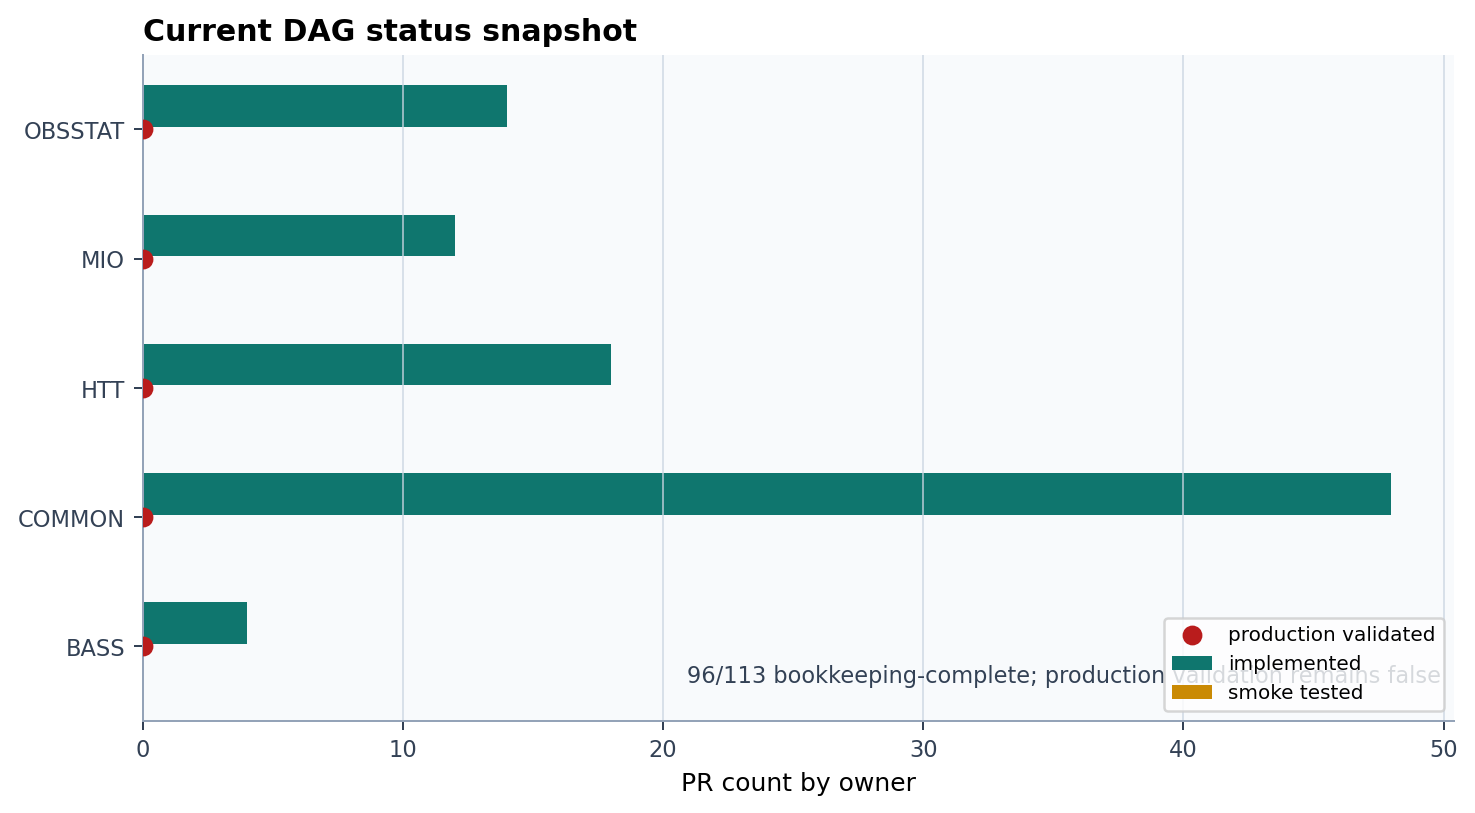
\includegraphics[width=0.92\textwidth]{current/fig_current_dag_progress}
\caption{Current DAG/status snapshot by repository owner. The panel is bookkeeping evidence only: completion and smoke status do not promote any result to production validation.}
\label{fig:current-dag-progress}
\end{figure}

\begin{figure}[htbp]
\centering
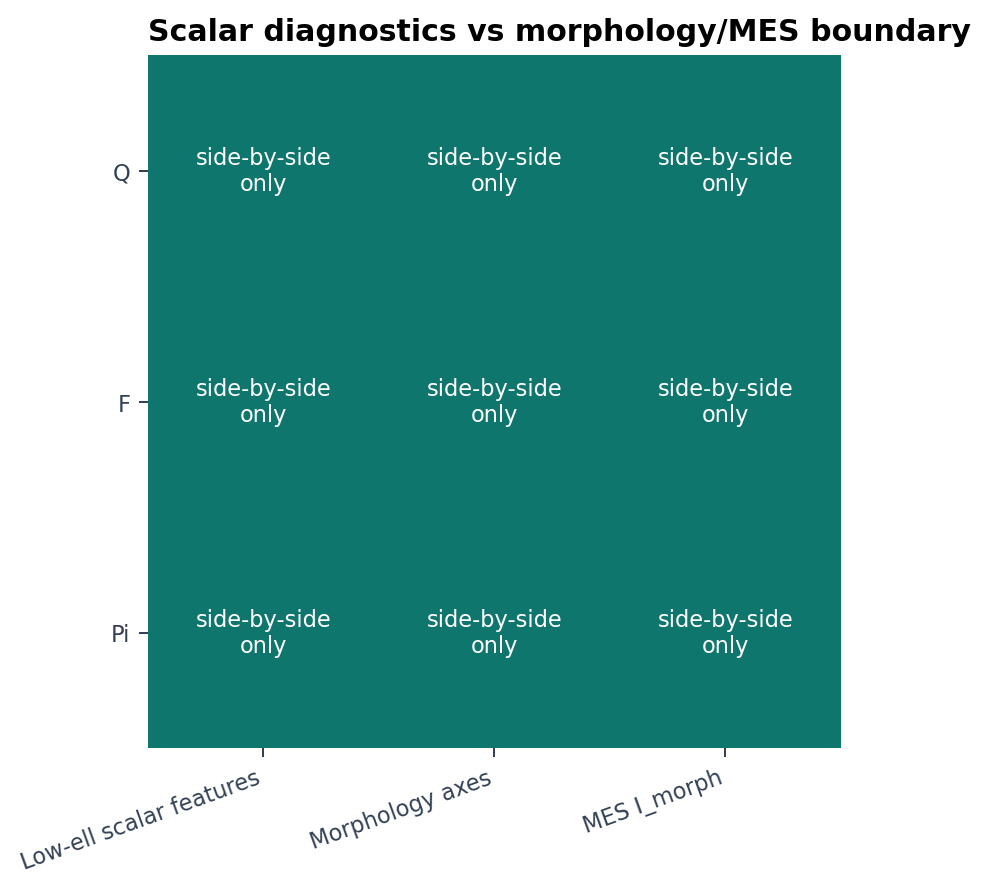
\includegraphics[width=0.92\textwidth]{current/fig_current_scalar_morphology_boundary}
\caption{Current scalar-to-morphology comparison matrix. The allowed state is diagnostic side-by-side reporting with separate provenance; scalar diagnostics and low-ell summaries do not identify geometry or provide Bianchi family-ID.}
\label{fig:current-scalar-morphology-boundary}
\end{figure}

% END current-code generated figure deck


% ── Chapter: Bianchi Bounds ───────────────────────────────────
% ============================================================
%  ch03_bianchi_bounds.tex — Bianchi Classification and Bounds
%  Requires: macros.tex, amsmath, amssymb, amsthm, booktabs
%  Estimated length: 25–35 pages
%  Rewritten: VD-08, 2026-03-07
% ============================================================

\chapter{Bianchi Type-by-Type Bounds}\label{ch:bianchi-bounds}

The master defect identity of Theorem~\ref{thm:master-defect-id}
provides the algebraic skeleton; the present chapter supplies the
numerical flesh.  We begin with a self-contained account of the
Bianchi classification (Section~\ref{sec:bianchi-class}), then
derive the MES three-bound hierarchy from the covariant Boltzmann
hierarchy (Section~\ref{sec:MES}), specialise the defect identity
to each of the nine types in both orthogonal and tilted sectors
(Sections~\ref{sec:BI}--\ref{sec:classAB}), analyse the Bianchi~V
momentum constraint in detail
(Section~\ref{sec:BV-tilt}), construct the four-dimensional
constraint space (Section~\ref{sec:4D}), and close with the
Frobenius shear--vorticity coupling
(Section~\ref{sec:frobenius-coupling}).


% ============================================================
\section{The Bianchi classification of spatially homogeneous
  spacetimes}\label{sec:bianchi-class}
% ============================================================

\subsection{Spatial Killing vectors and the isometry group}
\label{sec:killing}

Our goal in this section is to classify all spatially
homogeneous---but generically anisotropic---cosmological
geometries.  A spacetime is \emph{spatially homogeneous} if it
admits a group of isometries $G_3$ acting simply transitively
on a family of spacelike hypersurfaces~$\Sigma_t$.  The group
orbits are the surfaces~$\Sigma_t$ themselves: every point on
$\Sigma_t$ can be reached from any other by a group element.  The
isometry group is three-dimensional (matching the dimension of
the spatial sections), and its Lie algebra is specified by the
structure constants $C^c{}_{ab}$ satisfying
\begin{equation}\label{eq:lie-bracket}
[\xi_a, \xi_b] = C^c{}_{ab}\,\xi_c\,,
\end{equation}
where $\{\xi_a\}_{a=1,2,3}$ is a basis for the Killing vector
fields tangent to~$\Sigma_t$.  The antisymmetry
$C^c{}_{ab} = -C^c{}_{ba}$ and the Jacobi identity
$C^e{}_{[ab}C^d{}_{c]e} = 0$ constrain the possible algebras.


\subsection{Decomposition of the structure constants}
\label{sec:struct-decomp}

Ellis \& MacCallum~\cite{EllisMacCallum1969} introduced the
canonical decomposition
\begin{equation}\label{eq:struct-constants}
C^{\alpha}{}_{\beta\gamma}
= \epsilon_{\beta\gamma\delta}\,n^{\alpha\delta}
  + \delta^{\alpha}_{[\beta}\,a_{\gamma]}\,,
\end{equation}
where $n^{\alpha\beta} = n^{(\alpha\beta)}$ is a symmetric
$3 \times 3$ matrix and $a_\alpha$ is a covector.  The Jacobi
identity requires
\begin{equation}\label{eq:jacobi}
n^{\alpha\beta}\,a_\beta = 0\,.
\end{equation}
The symmetric matrix $n^{\alpha\beta}$ can always be
diagonalised; we write its eigenvalues as $(n_1, n_2, n_3)$.
The covector $a_\alpha$ is either zero or, by
Eq.~\eqref{eq:jacobi}, orthogonal to the image of~$n$.

The Bianchi types divide into two classes:
\begin{equation}
\text{Class A:}\quad a_\alpha = 0\,;\qquad
\text{Class B:}\quad a_\alpha \neq 0\,.
\end{equation}
Class~A models have unimodular group actions (the structure
constants satisfy $C^\alpha{}_{\alpha\beta} = 0$); Class~B
models do not.


\subsection{The nine Bianchi types}\label{sec:nine-types}

The possible combinations of $(n_1, n_2, n_3)$ and
$a = |a_\alpha|$ yield nine algebraically distinct Lie algebras.
We collect the complete classification in
Table~\ref{tab:bianchi-types}.

\begin{table}[ht]
\caption{Bianchi classification.  The eigenvalues $(n_1, n_2, n_3)$
of the symmetric part $n^{\alpha\beta}$ and the magnitude
$a = |a_\alpha|$ of the covector determine the type.  The
parameter $h$ in types VI$_h$ and VII$_h$ is the group parameter
$h = a^2/n_1 n_2$ (with $n_3 = 0$); type~III coincides
with~VI$_{-1}$.  The column ``$\Omega_k$ sign'' indicates the sign of
the curvature density parameter $\Omega_k = -\sR/(6\Htheta^2)$ under the
Ellis--MacCallum
convention~\eqref{eq:Rstar-bianchi}: since $\Omega_k = -\sR/(6\Htheta^2)$,
we show the sign of~$\Omega_k$: $0$ (flat), $-$ (open,
$k=-1$ FLRW limit), $+$ (closed, $k=+1$ limit).}
\label{tab:bianchi-types}
\centering\footnotesize\setlength{\tabcolsep}{3.5pt}
\begin{tabular}{llcccccc}
\toprule
Type & Class & $n_1$ & $n_2$ & $n_3$ & $a$
  & $\Omega_k$ sign & FLRW limit \\
\midrule
I      & A & $0$ & $0$ & $0$ & $0$
  & $0$ & $k = 0$ \\
II     & A & $+$ & $0$ & $0$ & $0$
  & $-$ & --- \\
VI$_0$ & A & $+$ & $-$ & $0$ & $0$
  & $-$ & --- \\
VII$_0$& A & $+$ & $+$ & $0$ & $0$
  & $-$ & $k = 0$ (special) \\
VIII   & A & $+$ & $+$ & $-$ & $0$
  & $\pm$ & --- \\
IX     & A & $+$ & $+$ & $+$ & $0$
  & $+$ & $k = +1$ \\
\midrule
III    & B & $+$ & $-$ & $0$ & $\neq 0$
  & $\pm$ & --- \\
IV     & B & $+$ & $0$ & $0$ & $\neq 0$
  & $-$ & --- \\
V      & B & $0$ & $0$ & $0$ & $\neq 0$
  & $-$ & $k = -1$ \\
VI$_h$ & B & $+$ & $-$ & $0$ & $\neq 0$
  & $\pm$ & --- \\
VII$_h$& B & $+$ & $+$ & $0$ & $\neq 0$
  & $-$ & $k = -1$ (special) \\
\bottomrule
\end{tabular}
\end{table}

Three types contain isotropic (FLRW) limits: Bianchi~I
($k = 0$), Bianchi~V ($k = -1$), and Bianchi~IX ($k = +1$),
each reached by setting all anisotropy to zero.  Bianchi~VII$_0$
also admits a flat FLRW limit as a special case, and VII$_h$
admits an open FLRW limit.  These are the types most relevant
for observational cosmology.


\subsection{Kinematic variables by type}\label{sec:kin-by-type}

Not every Bianchi type supports all four kinematic degrees of
freedom.  In the orthogonal sector ($\beta = 0$), the
geometry-frame congruence $u^a$ is the group-orbit normal,
giving $\omega_{ab}^{(G)} = 0$ and $\dot{u}_a^{(G)} = 0$
for all types---the only non-trivial kinematic variable is the
shear $\sigma_{ab}$.  The number of independent shear components
depends on the type (from $1$ for the LRS types to $5$ for the
fully anisotropic types).

Tilting the fluid activates additional variables: the tilt
rapidity $\beta$ and, through the King--Ellis boost
(Section~\ref{sec:king-ellis}), the matter-frame
vorticity $\hat{\omega}_{ab}$ and acceleration
$\hat{\dot{u}}_a$.  The vorticity generated by tilt depends on
the Bianchi type through the structure constants: King \&
Ellis~\cite{KingEllis1973} proved that the tilted fluid has
non-zero vorticity if and only if $n_{\alpha\beta}v^\alpha
\neq 0$, where $v^\alpha$ is the tilt velocity.

For Bianchi~I ($n_{\alpha\beta} = 0$), tilt cannot generate
vorticity regardless of the tilt direction.  For types with
non-degenerate $n_{\alpha\beta}$ (VII$_0$, VIII, IX), vorticity
is generically non-zero for any tilt direction not aligned with
a principal axis.  Type~V ($n_{\alpha\beta} = 0$) produces no
vorticity from the $n$-tensor route, but the non-zero
$a_\alpha$ creates a momentum constraint that algebraically
couples shear to tilt
(Section~\ref{sec:BV-tilt}).

Table~\ref{tab:kin-by-type} summarises the active variables
for each type.

\begin{table}[ht]
\caption{Active kinematic variables by Bianchi type.
``$\sigma$'': shear (present for all types, 1--5 independent
components). ``$\omega$'': matter-frame vorticity generated by
tilt. ``$\dot{u}$'': matter-frame four-acceleration (present
whenever $\beta \neq 0$ and $w \neq 0$). ``$\beta$'': tilt
rapidity. ``C'': tilt constrained by momentum equation.
``F'': tilt free.}
\label{tab:kin-by-type}
\centering\footnotesize\setlength{\tabcolsep}{4pt}
\begin{tabular}{lcccccl}
\toprule
Type & $\sigma$ & $\omega$ (orth.) & $\omega$ (tilted)
  & $\dot{u}$ (tilted) & $\beta$ & Notes \\
\midrule
I      & $\checkmark$ & --- & ---
  & $\checkmark$ & F & No vorticity from tilt \\
II     & $\checkmark$ & --- & $\checkmark$
  & $\checkmark$ & F & 1 tilt component \\
V      & $\checkmark$ & --- & ---
  & $\checkmark$ & C & $\Sigma^2 \propto \beta^2/\Omega_K$ \\
VII$_0$& $\checkmark$ & --- & $\checkmark$
  & $\checkmark$ & F & Generic vorticity \\
VII$_h$& $\checkmark$ & $\checkmark$ & $\checkmark$
  & $\checkmark$ & F & Frobenius: $\Wstd = R^2\Sigstd$ \\
IX     & $\checkmark$ & --- & $\checkmark$
  & $\checkmark$ & F & Generic vorticity \\
\bottomrule
\end{tabular}
\end{table}


% ============================================================
\section{The MES bound hierarchy}\label{sec:MES}
% ============================================================

\subsection{The covariant Boltzmann hierarchy}
\label{sec:boltzmann}

Before diving into the bound derivation, we set up the
Boltzmann equation for the photon distribution function in the
1+3 covariant formalism.  The CMB temperature observed by a
fundamental observer in sky direction $e^a$ (with
$e_a u^a = 0$, $e_a e^a = 1$) is
\begin{equation}\label{eq:T-expansion}
T(x^a, e^b) = \bar{T}(x)\Bigl[
  1 + \sum_{\ell \geq 1}
    \tau_{A_\ell}(x)\,e^{A_\ell}
\Bigr]\,,
\end{equation}
where $\tau_{A_\ell} = \tau_{\langle a_1 a_2 \cdots a_\ell
\rangle}$ are the PSTF temperature anisotropy multipoles and
$e^{A_\ell} = e^{\langle a_1}\cdots e^{a_\ell\rangle}$.  The
dimensionless smallness parameters are
\begin{equation}\label{eq:eps-def}
\eps_\ell := |\tau_{A_\ell}|
= (\tau_{A_\ell}\,\tau^{A_\ell})^{1/2} \ll 1\,.
\end{equation}

The energy-integrated intensity multipoles $I_{A_\ell}$ are
related to the temperature multipoles by $I_{A_\ell}/I \approx
4\,\tau_{A_\ell}$ (at linear order), where
$I \propto \bar{T}^4 \propto \rho_\gamma$ is the radiation
monopole.  The Boltzmann equation, projected into PSTF
multipoles, yields the \emph{multipole divergence equations}
(MDEs)~\cite{MaartensGE1999,ChallinorLasenby1999}:
\begin{equation}\label{eq:MDE-general}
\dot{I}_{A_\ell}
+ \tfrac{4}{3}\Theta\,I_{A_\ell}
+ \tilde{D}^b I_{bA_\ell}
- \frac{\ell}{2\ell+1}\,\tilde{D}_{\langle a_\ell}
  I_{A_{\ell-1}\rangle}
+ \tfrac{4}{3}\,I\,\dot{u}_{a_1}\,\delta_{\ell 1}
- \tfrac{8}{15}\,I\,\sigma_{a_1 a_2}\,\delta_{\ell 2}
= \mathcal{C}_{A_\ell}\,,
\end{equation}
where $\mathcal{C}_{A_\ell}$ denotes Thomson scattering terms.
Two features of this hierarchy are central to the MES programme:

(a) The \textbf{shear} $\sigma_{ab}$ enters \emph{only} in the
$\ell = 2$ equation, through the coefficient $8/15$.

(b) The \textbf{four-acceleration} $\dot{u}_a$ enters
\emph{only} in the $\ell = 1$ equation, through the coefficient
$4/3$.

Vorticity does not appear in the photon energy equation at all
(because $\omega_{ab}e^a e^b = 0$ by antisymmetry); it enters
only through the direction equation and the Einstein constraint
equations, making its bound structurally different from the
other two.


\subsection{Explicit transport equations for $\ell = 0, 1, 2, 3$}
\label{sec:transport}

We write out the first four levels of the hierarchy explicitly
(dropping scattering terms for the free-streaming regime after
decoupling):
\begin{align}
\ell = 0:\quad
& \dot{I} + \tfrac{4}{3}\Theta\,I
  + \tilde{D}^a I_a = 0\,,
  \label{eq:ell0}\\[4pt]
\ell = 1:\quad
& \dot{I}_a + \tfrac{4}{3}\Theta\,I_a
  + \tilde{D}^b I_{ab}
  - \tfrac{1}{3}\tilde{D}_a I
  + \tfrac{4}{3}\,I\,\dot{u}_a = 0\,,
  \label{eq:ell1}\\[4pt]
\ell = 2:\quad
& \dot{I}_{ab} + \tfrac{4}{3}\Theta\,I_{ab}
  + \tilde{D}^c I_{cab}
  - \tfrac{2}{5}\tilde{D}_{\langle a} I_{b\rangle}
  - \tfrac{8}{15}\,I\,\sigma_{ab} = 0\,,
  \label{eq:ell2}\\[4pt]
\ell = 3:\quad
& \dot{I}_{abc} + \tfrac{4}{3}\Theta\,I_{abc}
  + \tilde{D}^d I_{dabc}
  - \tfrac{3}{7}\tilde{D}_{\langle a} I_{bc\rangle}
  = 0\,.
  \label{eq:ell3}
\end{align}
The structure is transparent: each $\ell$ equation couples the
$\ell$-th multipole to its neighbours $\ell \pm 1$ through the
spatial gradient terms $\tilde{D}$.  The kinematic source terms
($\dot{u}_a$ at $\ell = 1$, $\sigma_{ab}$ at $\ell = 2$) break
the otherwise homogeneous hierarchy.


\subsection{The Copernican extension postulate}
\label{sec:copernican}

The MES bounds require not merely that \emph{we} observe
near-isotropy, but that \emph{all} fundamental observers do.
The precise statement, following Stoeger, Maartens \&
Ellis~\cite{StoegerME1995}, is:

\medskip
\noindent\textbf{Copernican Extension Postulate.}\quad
\textit{For all fundamental observers and for all $\ell \geq 1$:
\begin{equation}\label{eq:copernican}
|\tau_{A_\ell}| = O(\eps)\,,\qquad
|\dot{\tau}_{A_\ell}| = O(\eps)\,,\qquad
|\tilde{D}_b\,\tau_{A_\ell}| = O(\eps)\,,
\end{equation}
where $\eps \ll 1$ is the CMB anisotropy parameter.}
\medskip

The derivative-boundedness conditions are essential.  Without
them, the spatial gradient terms in
Eqs.~\eqref{eq:ell1}--\eqref{eq:ell3} are unconstrained, and
the shear inversion from the $\ell = 2$ equation fails.  The
Nilsson--Uggla--Wainwright counter-examples
(Section~\ref{sec:intro-EGS} of Chapter~\ref{ch:intro})
demonstrate precisely this failure mode: almost-isotropic CMB
with unbounded Weyl curvature, violating the derivative
condition.


\subsection{Derivation of the MES shear bound}
\label{sec:MES-shear-derivation}

We now derive the shear bound from the $\ell = 2$
equation~\eqref{eq:ell2}.  Solving for the shear:
\begin{equation}\label{eq:sigma-from-ell2}
\sigma_{ab}
= \frac{15}{8\,I}\Bigl[
  -\dot{I}_{ab} - \tfrac{4}{3}\Theta\,I_{ab}
  - \tilde{D}^c I_{cab}
  + \tfrac{2}{5}\tilde{D}_{\langle a} I_{b\rangle}
\Bigr]\,.
\end{equation}
Under the Copernican postulate, each term on the right-hand
side is $O(\eps)\,\Theta$ (using $I_{ab}/I \sim \eps_2$,
$\dot{I}_{ab}/I \sim \eps_2\,\Theta$, and the gradient
terms involving $\eps_1$ and $\eps_3$).  Taking norms:
\begin{equation}\label{eq:sigma-bound-raw}
\frac{\sqrt{\sigma_{ab}\sigma^{ab}}}{\Theta}
\leq \frac{15}{8}\Bigl[
  c_0\,\eps_2 + c_0'\,\eps_2
  + c_3\,\eps_3 + c_1\,\eps_1
\Bigr]\,,
\end{equation}
where the coefficients $c_0, c_0', c_3, c_1$ arise from the
PSTF Clebsch--Gordan coupling structure of the gradient terms.

In the \textbf{homogeneous case} (Bianchi models), all spatial
gradient terms vanish ($\tilde{D}_a = 0$ on the group orbits),
and the bound tightens dramatically: $\sigma/\Theta \sim
O(\eps_2)$ directly from the quadrupole.  In the
\textbf{inhomogeneous case}, the gradient terms
$\tilde{D}_{\langle a}I_{b\rangle}$ and
$\tilde{D}^c I_{cab}$ contribute terms proportional to
$\eps_1$ and $\eps_3$ respectively, yielding the weaker but
more general bound.

The MES result, combining the numerical prefactors from the
PSTF algebra (the Clebsch--Gordan coefficients for rank-2
coupling to $\ell = 1, 2, 3$), is:

\begin{theorem}[MES shear bound {\normalfont
  $[\ConditionalStatus]$}]\label{thm:MES-shear}
In any almost-FLRW cosmology satisfying:
\begin{enumerate}
\item[\emph{(A1)}] the almost-FLRW linearisation
  ($\sigma/\Theta \ll 1$, $\omega/\Theta \ll 1$),
\item[\emph{(A2)}] the Copernican extension postulate
  (observed multipoles are representative of the full sky),
\item[\emph{(A3)}] the PSTF truncation at $\ell \leq 3$
  (higher multipoles contribute only through the next-order
  coupling, which is suppressed by $\eps_4/\eps_1
  \sim 10^{-3}$),
\end{enumerate}
we have
\begin{equation}\label{eq:Bsig-def}
\frac{\sqrt{\sigma_{ab}\sigma^{ab}}}{\Theta}
< \Bsig
:= \tfrac{5}{3}\,\eps_1 + 3\,\eps_2 + \tfrac{3}{7}\,\eps_3\,.
\end{equation}
\end{theorem}

The coefficients have the following origin:
$5/3$ is the PSTF coupling of the rank-2 shear to the
rank-1 dipole through the gradient
$\tilde{D}_{\langle a}I_{b\rangle}$, involving the
Gaunt coefficient $\langle 1\,0;\,2\,0|1\,0\rangle$;
$3$ is the direct $\ell = 2$ coefficient from the
$I_{ab}$ term in Eq.~\eqref{eq:sigma-from-ell2};
$3/7$ is the coupling to the octupole through
$\tilde{D}^c I_{cab}$, involving the Gaunt coefficient
$\langle 3\,0;\,2\,0|3\,0\rangle$.

\paragraph{Dipole dominance.}
At Planck sensitivity, $\eps_1 \approx 1.234 \times 10^{-3}$
while $\eps_2 \approx 3.56 \times 10^{-6}$ and
$\eps_3 \approx 6.07 \times 10^{-6}$.  The three contributions
to $\Bsig$ are:
\begin{equation}\label{eq:dipole-dominance}
\tfrac{5}{3}\eps_1 = 2.057 \times 10^{-3}\,,\quad
3\eps_2 = 1.068 \times 10^{-5}\,,\quad
\tfrac{3}{7}\eps_3 = 2.600 \times 10^{-6}\,,
\end{equation}
giving $\Bsig = 2.069 \times 10^{-3}$.  The dipole term
contributes $2.057/2.069 = 99.4\%$ of the total.  The shear
bound is, for all practical purposes, a dipole bound.


\subsection{Vorticity and acceleration bounds}
\label{sec:om-udot-bounds}

The vorticity and acceleration bounds follow from the same
Boltzmann hierarchy but through different coupling pathways.

\paragraph{Vorticity bound.}
Vorticity does not appear directly in the photon energy
equation---the contraction $\omega_{ab}e^a e^b$ vanishes
identically by antisymmetry.  The vorticity bound is derived
indirectly, through the Einstein constraint equations.  The
momentum constraint (the $G_{0i}$ field equation) links the
divergence of the shear to the vorticity:
\begin{equation}\label{eq:momentum-constraint}
\tilde{D}^b\sigma_{ab} - \tfrac{2}{3}\tilde{D}_a\Theta
+ \eta_{abc}(\tilde{D}^b\omega^c + 2\dot{u}^b\omega^c)
+ \kappa\,q_a = 0\,.
\end{equation}
Since $\sigma/\Theta = O(\eps)$ and $\dot{u}/\Theta = O(\eps)$
from the shear and acceleration bounds, and the spatial gradients
are bounded by the Copernican postulate, the constraint
propagates the smallness to $\omega/\Theta$.

\begin{theorem}[MES vorticity bound {\normalfont
  $[\ConditionalStatus]$}]\label{thm:MES-omega}
Under the same conditions as Theorem~\ref{thm:MES-shear},
\begin{equation}\label{eq:Bom-def}
\frac{\sqrt{\omega_{ab}\omega^{ab}}}{\Theta}
< \Bom
:= \tfrac{3}{4}\,\eps_1 + 2\,\eps_2 + \tfrac{2}{7}\,\eps_3\,.
\end{equation}
\end{theorem}

The coefficients $(3/4, 2, 2/7)$ arise from the $\Delta\ell =
\pm 1$ coupling of the vorticity vector (rank-1 spatial tensor)
with the photon multipoles, propagated through the constraint
equations.  The vorticity bound is logically \emph{dependent}
on the shear and acceleration bounds---it requires establishing
$\sigma = O(\eps)\Theta$ and $\dot{u} = O(\eps)\Theta$ first,
then using the Einstein constraints to close the system.

\paragraph{Acceleration bound.}
The acceleration enters the $\ell = 1$
equation~\eqref{eq:ell1} through the coefficient $4/3$.
Inverting:
\begin{equation}\label{eq:udot-from-ell1}
\dot{u}_a = \frac{3}{4\,I}\Bigl[
  -\dot{I}_a - \tfrac{4}{3}\Theta\,I_a
  - \tilde{D}^b I_{ab}
  + \tfrac{1}{3}\tilde{D}_a I
\Bigr]\,.
\end{equation}

\begin{theorem}[MES acceleration bound {\normalfont
  $[\ConditionalStatus]$}]\label{thm:MES-udot}
Under the same conditions,
\begin{equation}\label{eq:Bud-def}
\frac{\sqrt{\dot{u}_a\dot{u}^a}}{\Theta}
< \Bud
:= \tfrac{3}{4}\,\eps_1 + \eps_2 + \tfrac{3}{14}\,\eps_3\,.
\end{equation}
\end{theorem}

The coefficient $3/4$ for $\eps_1$ arises from the monopole--dipole
coupling induced by the acceleration source term in
Eq.~\eqref{eq:ell1}; the coefficient $1$ for $\eps_2$ comes from
the gradient term $\tilde{D}^b I_{ab}$; and $3/14$ for $\eps_3$
involves the next-order gradient coupling.


\subsection{Bound ordering hierarchy}\label{sec:hierarchy}

\begin{proposition}[Bound ordering {\normalfont
  $[\ConditionalStatus]$}]\label{prop:ordering}
For any set of non-negative CMB multipoles
$(\eps_1, \eps_2, \eps_3)$:
\begin{enumerate}
\item[\emph{(i)}]
  \textbf{Weak hierarchy} (requires only $\eps_1 > 0$):
  \begin{equation}\label{eq:ordering-weak}
  \Bsig > \Bom \geq \Bud\,.
  \end{equation}
\item[\emph{(ii)}]
  \textbf{Strict hierarchy} (requires $\eps_2 > 0$ or
  $\eps_3 > 0$):
  \begin{equation}\label{eq:ordering-strict}
  \Bsig > \Bom > \Bud\,.
  \end{equation}
\end{enumerate}
\end{proposition}

\begin{proof}
For $\Bsig > \Bom$: the $\eps_1$ coefficients are
$5/3 > 3/4$, so $\eps_1 > 0$ alone suffices.  For
$\Bom \geq \Bud$: the $\eps_1$ coefficients are equal
($3/4 = 3/4$), and the remaining coefficients satisfy
$2 \geq 1$ ($\eps_2$) and $2/7 \geq 3/14$ ($\eps_3$).
This gives part~(i).  Strict inequality $\Bom > \Bud$
requires at least one of $\eps_2 > 0$ or $\eps_3 > 0$,
since the $\eps_2$ coefficient is $2 > 1$ and the $\eps_3$
coefficient is $2/7 > 3/14$.  Planck measures $\eps_2 > 0$,
so part~(ii) holds observationally.
\end{proof}

\begin{remark}[Near-degeneracy of the lower hierarchy]
\label{rem:lower-degeneracy}
The gap between the two lower bounds is
$\Bom - \Bud = \eps_2 + \eps_3/14$.
Strictness therefore requires only that $\eps_2 > 0$
\emph{or} $\eps_3 > 0$; the condition $\eps_2 > 0$ stated
above is sufficient but not necessary.  In the observational
regime $(\eps_2, \eps_3) \ll \eps_1$, this gap is
$\sim 4 \times 10^{-6}$, so the lower hierarchy
$\Bom \gtrsim \Bud$ is numerically near-degenerate even
when strictly ordered.
\end{remark}

The physical content is that the CMB is most
sensitive to shear (rank-2, direct quadrupole source) and least
sensitive to acceleration (rank-1, entering through
monopole--dipole coupling).  The hierarchy is preserved under
dynamical evolution
(Remark~\ref{rem:hierarchy-conservation} of
Chapter~\ref{ch:framework}).
the conditioned legacy figure gallery in Appendix~\ref{app:conditioned-legacy-figure-gallery} shows the three bounds as
functions of the observed multipole amplitudes $(\eps_1,
\eps_2, \eps_3)$, with the strict hierarchy
$\Bsig > \Bom > \Bud$ visible across the full observational range.


\subsection{Standardised-variable form and frame correction}
\label{sec:std-form}

From the definitions $\Sigstd = \sigma_{ab}\sigma^{ab}/(6\Htheta^2)$
and $\Htheta = \Theta/3$, we have
$(\sigma/\Theta)^2 = (2/3)\Sigstd$, giving:
\begin{equation}\label{eq:Sig2-from-Bsig}
\Sigstd < \tfrac{3}{2}\,\Bsig^2\,,\qquad
\Wstd < \tfrac{3}{2}\,\Bom^2\,,\qquad
\Astd < \tfrac{3}{2}\,\Bud^2\,.
\end{equation}

For tilted models, the observed $\eps_1$ contains the
acceleration contribution
$\eps_1^{(\dot{u})} = \etaud\beta$
(Section~\ref{sec:accel-dipole}).  Using the corrected
safe-route $\beta \leq \eps_1/(1 + \etaud)$ and the fact that
$\Bsig$ is linear in $\eps_1$, the frame-corrected bound is
\begin{equation}\label{eq:Bsig-corr}
\Bsig^{\mathrm{corr}}
= \Bsig(\eps_1) + \tfrac{5}{3}\,\etaud\,\beta
\approx (1 + 2.69\,\eps_1)\,\Bsig\,.
\end{equation}
The correction factor $R = 1 + 2.69\eps_1$ produces a
$\sim 0.4\%$ effect on $\Bsig$ and a $\sim 0.8\%$ effect on
$\Sigstd$, propagating to $\sim 16\%$ on $\xmax$ for
shear-dominated types (since $\xmax \propto \Bsig^2$).

The frame-attribution bias $\Bbias = \Bsig^{\mathrm{corr}} -
\Bsig$ must be reported alongside $\Bsig$ values in all
subsequent analysis, per the VT-07 mandate.


% ============================================================
\section{Bianchi~I: the minimal benchmark}\label{sec:BI}
% ============================================================

Bianchi~I is the simplest anisotropic cosmology: flat spatial
sections with no vorticity and no spatial curvature.  The
structure constants vanish entirely ($n^{\alpha\beta} = 0$,
$a_\alpha = 0$), giving $\sR = 0$ and $\Omega_k = 0$.

\begin{theorem}[Bianchi~I defect identity {\normalfont $[\ExactStatus]$}]
\label{thm:BI-defect}
For orthogonal Bianchi~I ($\beta = 0$), $\xI = \Sigstd$.
For tilted Bianchi~I, $\xI = \Sigstd + \Otilt$.
\end{theorem}

\begin{proof}
We apply Theorem~\ref{thm:master-defect-id} with the flat
comparator ($\Okref = 0$).  Since $\Omega_k = 0$ for type~I,
$\Okaniso = \Omega_k - \Okref = 0$.  In the orthogonal sector,
$\beta = 0$ gives $\Otilt = 0$, and $\omega_{ab}^{(G)} = 0$
gives $\Wstd = 0$.  The identity reduces to
$\xI = \Sigstd$.  For tilted type~I, $\Otilt =
(1+w)\Omega_m\sinh^2\!\beta > 0$ while $\Wstd$ remains zero
(type~I cannot generate matter-frame vorticity because
$n_{\alpha\beta} = 0$).  Hence $\xI = \Sigstd + \Otilt$.
\end{proof}

The observational bound follows immediately:
$\xI < (3/2)\Bsig^2$ (orthogonal) or
$\xI < (3/2)[\Bsig^{\mathrm{corr}}]^2 + \Otilt(\betasr)$
(tilted).  At the S3 scenario, the orthogonal bound gives
$\xI < 6.42 \times 10^{-6}$.

Bianchi~I serves as the \emph{minimal anisotropy benchmark}
in the irrotational non-negative sector: for flat orthogonal
types (BVII$_0$, BII, BVI$_0$) under the flat comparator,
$x = \Sigstd = \xI$.  This ordering does \emph{not} hold
generally: types with negative $\Okaniso$ (BVIII, BIX under
the flat comparator) can have $x < 0 < \xI$, and tilted BI
itself has $x = \Sigstd + \Otilt > \xI$ (the tilt raises the
defect above the pure-shear level).

For tilted Bianchi~I, the geometry-frame vorticity vanishes
($\omega_{ab}^{(G)} = 0$) because the structure constants are
trivial.  The matter-frame vorticity is also zero in LRS
(locally rotationally symmetric) tilted type~I, but can be
non-zero in the generic (non-LRS) tilted case when the tilt
axis is not aligned with a shear eigenaxis~\cite{King1973}.
We restrict to the LRS case throughout this analysis.


% ============================================================
\section{Tilted Bianchi~V and the momentum constraint}
\label{sec:BV-tilt}
% ============================================================

Bianchi~V occupies a distinguished position: it is the unique
type for which tilt is not a free parameter but is
\emph{geometrically constrained} by the momentum equations.
This constraint leads to a quadrupole overproduction that
excludes Bianchi~V as a viable cosmological model at any tilt
consistent with the observed dipole anomaly.


\subsection{Geometric structure}\label{sec:BV-geom}

The type~V structure constants are $n^{\alpha\beta} = 0$ and
$a_\alpha \neq 0$ (Class~B).  The spatial Ricci scalar is
$\sR = 4\,a_\alpha a^\alpha > 0$, corresponding to open
spatial sections with $\Omega_k = -\sR/(6\Htheta^2) < 0$.
The isotropic limit ($\sigma_{ab} = 0$, $\beta = 0$) is the
$k = -1$ FLRW model.

A key algebraic property distinguishes type~V from all other
curved types: the traceless spatial Ricci tensor ${}^*\!S_{ab}$
vanishes identically:
\begin{equation}\label{eq:BV-Sab}
{}^*\!S_{ab} := {}^*\!R_{\langle ab\rangle}
= {}^*\!R_{ab} - \tfrac{1}{3}\sR\,h_{ab} = 0\,.
\end{equation}
This vanishing follows because $n^{\alpha\beta} = 0$: the spatial
curvature is isotropic.  The consequence for the defect identity
is immediate: using the open comparator
$\Okref = \Omega_k^{(\mathrm{BV})}$, we have $\Okaniso = 0$.
The defect reduces to
$\xV = \Sigstd - \Wstd + \Otilt$.
Since type~V with $n_{\alpha\beta} = 0$ generates no
matter-frame vorticity from tilt (the King--Ellis condition
$n_{\alpha\beta}v^\alpha = 0$ is trivially satisfied), we have
$\Wstd = 0$ and
\begin{equation}\label{eq:xV-simple}
\xV = \Sigstd + \Otilt\,.
\end{equation}


\subsection{The momentum constraint}\label{sec:BV-momentum}

The Einstein $G_{0i}$ field equations for Bianchi~V impose a
constraint that algebraically couples the shear to the tilt.
In the DCP notation of
Krishnan~et~al.~\cite{Krishnan2022,Krishnan2023}, the
momentum constraint reads
\begin{equation}\label{eq:BV-momentum-DCP}
\frac{2A_0}{X}\Bigl(\frac{\dot{X}}{X}
  - \frac{\dot{Y}}{Y}\Bigr)
= (\rho + p)\,\sinh\beta\,\cosh\beta\,.
\end{equation}
The left-hand side is proportional to the shear
($\sigma_{\mathrm{DCP}} = \dot{X}/X - \dot{Y}/Y$), and
$A_0$ encodes the spatial curvature ($\Omega_K \propto
A_0^2/X^2$).  We now convert to standardised variables.

The LRS Bianchi~V shear satisfies
$\sigma_{ab}\sigma^{ab} = 2\sigma^2 = \frac{2}{3}\sigma_{\mathrm{DCP}}^2$
(the factor $2/3$ from the diagonal traceless shear in three
dimensions), so $\Sigstd = \sigma_{\mathrm{DCP}}^2/(6\Htheta^2)$.
From Eq.~\eqref{eq:BV-momentum-DCP}, squaring both sides and
converting:
\begin{equation}\label{eq:BV-Sig2-exact}
\Sigstd
= \frac{[(1+w)\,\Omega_m]^2\,\sinh^2\!\beta\,\cosh^2\!\beta}
       {4\,|\Omega_K|}\,.
\end{equation}
For $\beta \ll 1$ (valid at the dipole-anomaly amplitude
$\beta \sim 10^{-3}$), $\sinh\beta\,\cosh\beta \approx \beta$,
and the constraint simplifies to
\begin{equation}\label{eq:BV-momentum}
\boxed{
\Sigstd
= \frac{[(1+w)\,\Omega_m]^2\,\beta^2}{4\,|\Omega_K|}
}\,.
\end{equation}
Note that $\Sigstd \propto \beta^2/|\Omega_K|$: the shear is
quadratic in the tilt and inversely proportional to the spatial
curvature.  For small curvature ($|\Omega_K| \ll 1$), a modest
tilt generates enormous shear.


\subsection{Quadrupole overproduction}\label{sec:BV-quad}

We now demonstrate that the momentum
constraint~\eqref{eq:BV-momentum} forces Bianchi~V to
overproduce the CMB quadrupole by a catastrophic margin.

At the CF4 tilt rapidity $\beta = 1.334 \times 10^{-3}$
(WFH2009 primary value; the CF4++ sensitivity variant
$\beta = 1.051 \times 10^{-3}$ gives
$\Sigstd \approx 2.74 \times 10^{-5}$---qualitatively
identical)
and the Planck-preferred curvature
$|\Omega_K| = 0.001$, with $w = 0$ (dust) and
$\Omega_m = 0.3153$:
\begin{equation}\label{eq:BV-Sig2-num}
\Sigstd
= \frac{(0.3153)^2 \times (1.334 \times 10^{-3})^2}
       {4 \times 0.001}
= \frac{1.773 \times 10^{-7}}{4 \times 10^{-3}}
\approx 4.43 \times 10^{-5}\,.
\end{equation}
The MES algebraic ceiling is
$\Sigmax = (3/2)\Bsig^2 \approx 6.42 \times
10^{-6}$.  The momentum-constrained value exceeds the MES
ceiling by a factor of $\sim 7$.

The situation is far worse when we compute the implied CMB
quadrupole.  Using the vector-mode transfer function
$T_2 = 5{,}247.5\;\mu\mathrm{K}/(\sigma/H)$ (VER05 corrected; see Appendix), the shear-induced quadrupole is
$D_2^{\mathrm{shear}} \sim T_2^2 \times \Sigstd$,\footnote{The pre-VER05 formula incorrectly included a factor of $T_0$; the corrected formula is $D_2^{\mathrm{shear}} = (6/2\pi)(T_2\,\sigma_H)^2$ where $T_2$ is in $\mu\mathrm{K}/(\sigma/H)$.}\, where $T_0^2
\sim 10^{15}\;\mu\mathrm{K}^2$---a $10^{13}$-fold
overproduction relative to the observed
$D_2^{\mathrm{obs}} = 225.9\;\mu\mathrm{K}^2$.

This overproduction is independent of the equation of state:
for radiation ($w = 1/3$), the prefactor $(1+w)^2$ increases by
$78\%$, worsening the exclusion.  Bianchi~V is
\emph{falsified by geometry}: there is no parameter-space region
that simultaneously accommodates the CF4 bulk flow and the
observed quadrupole.

\begin{remark}[Tilt bound from the momentum constraint
  {\normalfont $[\ConditionalStatus]$}]
\label{rem:BV-tilt-bound}
Under the following conditions---LRS (locally rotationally
symmetric) geometry, single perfect fluid ($w = 0$), DCP
(deparametrised Copernican principle) dictionary connecting
$\Sigstd$ to $D_2$, and small-$\beta$ linearisation---the
momentum constraint~\eqref{eq:BV-momentum} can be read as
an \emph{upper bound on $\beta$} for a given $\Sigstd$:
$\beta \leq 2\sqrt{|\Omega_K|\,\Sigstd}/[(1+w)\Omega_m]$.
At the MES ceiling $\Sigstd = (3/2)\Bsig^2$ and the Planck-preferred
$|\Omega_K| = 0.001$, the maximum tilt is
$\beta_{\mathrm{BV}} \approx 5.1 \times 10^{-4}$,
which is $\sim 2.2$ times tighter than the safe-route bound
$\betasr = 1.14 \times 10^{-3}$.  The constraint becomes
dramatically stronger for smaller $|\Omega_K|$: at
$|\Omega_K| = 10^{-4}$, the ratio rises to $\sim 7$.  In all
cases, the momentum constraint effectively removes Bianchi~V
from the set of viable tilted cosmologies because the
\emph{implied shear} at the CF4 tilt rapidity exceeds the MES
ceiling by a factor of $\sim 7$.
\end{remark}


% ============================================================
\section{Bianchi~VII$_h$: the richest geometry}
\label{sec:BVIIh}
% ============================================================

Type~VII$_h$ admits shear, vorticity, curvature, and a
``spiral'' parameter $x_h = \sqrt{h}/\sqrt{|\Omega_K|}$
that controls the scale of the helical pattern in the CMB.
The structure constants have $n^{\alpha\beta} =
\mathrm{diag}(n_1, n_2, 0)$ with $n_1, n_2 > 0$, and
$a_\alpha \neq 0$ with $h = a^2/(n_1 n_2)$ defining the
group parameter.


\subsection{Vorticity--shear coupling (Frobenius)}
\label{sec:VIIh-frobenius}

The Jacobi identities for type~VII$_h$ impose an algebraic
relation between the vorticity and shear.  For the LRS
(locally rotationally symmetric) sector, the Wainwright--Ellis
constraint gives
\begin{equation}\label{eq:WS-coupling}
\Wstd = R_{\mathrm{WS}}^2\,\Sigstd\,,
\end{equation}
where $R_{\mathrm{WS}}$ depends on the ratio $h/|\Omega_K|$.
For the observationally preferred range
($h/|\Omega_K| \in [0.1, 10]$),
$R_{\mathrm{WS}} \in [0.9, 1.2]$; the reference value used
throughout this work is $R_{\mathrm{WS}} = 1.06$.

The coupling~\eqref{eq:WS-coupling} means that any constraint
on the vorticity automatically tightens the shear bound and
vice versa.  The Saadeh 95\% upper limit
$(\omega/H)_0 < 5.2 \times 10^{-11}$, translating to
$\Wstd < 9.01 \times 10^{-22}$
(Eq.~\eqref{eq:omH-W2}), then implies
\begin{equation}\label{eq:Sig-from-Saa}
\Sigstd < \frac{\WSaa}{R_{\mathrm{WS}}^2}
= \frac{9.01 \times 10^{-22}}{1.12}
\approx 8.04 \times 10^{-22}\,.
\end{equation}
Equation~\eqref{eq:Sig-from-Saa} is the tightest model-dependent constraint on shear in
the entire Bianchi classification, achieved not by a direct
shear measurement but by the geometric coupling that transmits
the vorticity bound to the shear sector---six orders of
magnitude tighter than the MES algebraic bound.


\subsection{Decay and growing modes}\label{sec:VIIh-modes}

The regular tensor mode in VII$_h$ admits two behaviours: a
decaying mode with transfer function
$T_2^{\mathrm{decay}} = 5{,}247.5\;\mu\mathrm{K}/(\sigma/H)$ and a growing
mode with $T_2^{\mathrm{grow}} = 1.05\;\mu\mathrm{K}/(\sigma/H)$
(VER05 BASS-calibrated values; $\pm 20\%$ calibration
uncertainty)~\cite{Saadeh2016b,Pontzen2011}.

The decaying mode produces a detectable CMB signal at
$(\sigma/H)_0 \sim 10^{-10}$, well below the MES algebraic
ceiling.  The growing mode, by contrast, requires
$(\sigma/H)_0 \sim 10^{-6}$ for a comparable signal---close
to the MES bound itself.  This growing mode is the unique
solution compatible with inflationary initial conditions
(Collins \& Hawking~\cite{CollinsHawking1973}), but its
associated vorticity (through the Frobenius coupling) exceeds
the Saadeh bound by orders of magnitude, leading to decisive
exclusion ($\ln\mathcal{B} = -18.7$) in the Bayesian analysis
(Chapter~\ref{ch:evidence}).

The Saadeh--MES complementarity is most visible for this type.
The $\sim 6$ order-of-magnitude gap between the Saadeh bound
($\Sigstd < 8 \times 10^{-22}$) and the MES algebraic bound
($\Sigstd < 6.4 \times 10^{-6}$) shrinks to approximately one
order for the regular tensor growing mode, where the transfer
function is $\sim 5000\times$ weaker and the dynamical lever arm
collapse.  The two frameworks are complementary: MES provides
type-independent algebraic ceilings; Saadeh~et~al.\ exploit
the full morphological information of the Planck sky.


\subsection{Tilted VII$_h$}\label{sec:VIIh-tilted}

Adding tilt to VII$_h$ introduces a four-parameter model
$(\Sigstd, \beta, \Wstd, x_h)$ that is the most complex in
the classification.  The vorticity Occam cost
($\sim 1.4$~nats) reduces the evidence relative to simpler
tilted types, but the model remains preferred over FLRW only in
the legacy transfer-conditional ranking
($\ln\mathcal{B} \approx +24$) in the evidence analysis
of Chapter~\ref{ch:evidence}.


% ============================================================
\section{Bianchi~IX: the closed model}\label{sec:BIX}
% ============================================================

Type~IX has closed spatial sections ($\sR < 0$ in the
Ellis--MacCallum convention, corresponding to $\Omega_k > 0$)
and admits a natural closed comparator
$\Okref = \Omega_k^{(\mathrm{IX})}$.


\subsection{Curvature split}

For the curvature-matched comparator, $\Okaniso = 0$ and the
defect reduces to $\xIX = \Sigstd + \Otilt$, identical in
form to Bianchi~I.  The distinction lies in the \emph{indirect}
effect of curvature: the Planck constraint
$|\Omega_K| < 0.002$ (95\% CL) limits the curvature contribution
to $\Okaniso \lesssim 10^{-3}$ under the flat comparator, but
under the matched comparator $\Okaniso$ vanishes by definition.

The Collins--Hawking theorem guarantees that all type~IX models
with $\Lambda > 0$ isotropise at late times.  In the concordance
model, the present-epoch shear is exponentially suppressed below
the MES bound, and the observational constraint is driven by the
tilt rapidity through the dipole anomaly.


\subsection{The orthogonal bound}

For orthogonal type~IX (no tilt), the defect with the flat
comparator is $\xIX = \Sigstd + \Okaniso$, where
$\Okaniso = \Omega_k > 0$.  Using the MES shear ceiling and the
Planck curvature prior:
\begin{equation}
\xIX < (3/2)\Bsig^2 + |\Omega_K|
\approx 6.42 \times 10^{-6} + 2 \times 10^{-3}
\approx 2 \times 10^{-3}\,.
\end{equation}
The curvature term dominates in the flat-comparator analysis.
Under the matched comparator, the bound drops to the
Bianchi~I value.


% ============================================================
\section{Remaining types}\label{sec:classAB}
% ============================================================

The six types not yet discussed decompose into two groups.

\subsection{Class~A types (II, VI$_0$, VII$_0$, VIII)}

Types~II, VI$_0$, VII$_0$, and~VIII are Class~A
($a_\alpha = 0$).  Each admits a curvature-matched comparator
for which $\Okaniso = 0$.  Their orthogonal defect bounds are
therefore identical to Bianchi~I up to the curvature matching.
For the flat comparator, types with non-zero $n^{\alpha\beta}$
acquire an $\Okaniso$ term that is generically small
($\lesssim 10^{-3}$) under Planck curvature priors.

In the tilted sector, all four types admit free tilt ($\beta$ is
not constrained by a momentum equation).  Types~II, VII$_0$,
and~VIII generate matter-frame vorticity through the tilt
(since $n_{\alpha\beta} \neq 0$), while type~VI$_0$ (with
$n_1 n_2 < 0$) admits vorticity generation for specific tilt
directions.


\subsection{Class~B types (III, IV, VI$_h$)}

Types~III, IV, and~VI$_h$ are Class~B ($a_\alpha \neq 0$).
The non-vanishing covector introduces a momentum constraint
that couples shear to tilt.  For type~V, this coupling is
algebraically exact (Section~\ref{sec:BV-tilt}).  For type~III
($= \mathrm{VI}_{-1}$), the constraint is weaker, allowing
independent variation of $\Sigstd$ and $\beta$.  Type~IV is
cosmologically marginal: it does not admit an FLRW limit and
is not considered further.


% ============================================================
\section{Summary of type-by-type bounds}\label{sec:summary}
% ============================================================

Table~\ref{tab:type-summary} collects the defect bounds for
all types under the S3 observational scenario, distinguishing
orthogonal and tilted sectors.

\begin{table}[ht]
\caption{Defect bounds by Bianchi type (S3 scenario,
$\eps_1 = 1.476 \times 10^{-3}$).  ``Orth.\ $x_{\max}$'':
orthogonal bound from MES algebraic ceiling.  ``Tilt'': F~=~free
parameter, C~=~constrained by momentum equation.
``Frobenius'': whether the Wainwright--Ellis
coupling~\eqref{eq:WS-coupling} applies.
All bounds include the VT-07 frame correction.}
\label{tab:type-summary}
\centering\footnotesize\setlength{\tabcolsep}{3.5pt}
\begin{tabular}{llccll}
\toprule
Type & Class & $\Omega_k$ sign
     & Orth.\ $x_{\max}$ & Tilt & Frobenius \\
\midrule
I       & A & $0$  & $(3/2)\Bsig^2$         & F  & --- \\
II      & A & $-$  & $(3/2)\Bsig^2$         & F  & --- \\
VI$_0$  & A & $-$  & $(3/2)\Bsig^2$         & F  & --- \\
VII$_0$ & A & $-$  & $(3/2)\Bsig^2$         & F  & --- \\
VIII    & A & $\pm$& $(3/2)\Bsig^2 + \Okaniso$ & F  & --- \\
IX      & A & $+$  & $(3/2)\Bsig^2 + \Okaniso$ & F  & --- \\
\midrule
III     & B & $\pm$& $(3/2)\Bsig^2 + \Okaniso$ & F  & --- \\
V       & B & $-$  & $(3/2)\Bsig^2$             & C  & --- \\
VII$_h$ & B & $-$  & $\WSaa/R_{\rm WS}^2$       & F  &
  $\Wstd = R_{\rm WS}^2\Sigstd$ \\
\bottomrule
\end{tabular}
\end{table}

The table reveals a clear trichotomy.  Types without curvature
(I, VII$_0$) have the simplest bounds.  Types with curvature
(II, III, V, VI$_0$, VIII, IX) acquire an $\Okaniso$ term
that is small under Planck priors.  Type~VII$_h$ alone has a
Frobenius coupling that tightens the bound by six orders of
magnitude.  the conditioned legacy figure gallery in Appendix~\ref{app:conditioned-legacy-figure-gallery} presents the
per-type evidence and departure summary that results from
applying this bound hierarchy to data.

\paragraph{Robustness.}

The type-by-type bounds in this chapter depend on the transport
hierarchy only through the orthogonal Thomson anchor and its
tilted-frame generalisation.  The latter is now isolated in the
Layer-B construction of Section~\ref{sec:tilted-thomson-layer-b},
where the $\beta \to 0$ byte-identity reduction to the LB-4
collision operator is enforced explicitly and the first
polarisation-rotation corrections are quantified on the same
PSTF basis used here.


% ============================================================
\section{The four-dimensional constraint space}
\label{sec:4D}
% ============================================================

\subsection{Constraint inventory}\label{sec:constraint-inventory}

The full constraint space is the region in
$(\Sigstd, \Wstd, \Astd, \beta)$ compatible with all
observational bounds.  We collect the constraints:
\begin{equation}\label{eq:constraint-inventory}
\begin{aligned}
\text{MES shear:} &\quad \Sigstd < \tfrac{3}{2}\Bsig^2\,,\\
\text{MES vorticity:} &\quad \Wstd < \tfrac{3}{2}\Bom^2\,,\\
\text{MES acceleration:} &\quad \Astd < \tfrac{3}{2}\Bud^2\,,\\
\text{Saadeh vorticity:} &\quad \Wstd < 9.01 \times 10^{-22}\,,\\
\text{Safe-route tilt:} &\quad \beta < \betasr\,,\\
\text{Frobenius (VII$_h$):} &\quad
  \Wstd = R_{\mathrm{WS}}^2\,\Sigstd\,,\\
\text{Momentum (V):} &\quad
  \Sigstd = [(1{+}w)\Omega_m]^2\beta^2/(4|\Omega_K|)\,.
\end{aligned}
\end{equation}


\subsection{Six-panel atlas}\label{sec:atlas}

The six independent two-dimensional projections of the
four-dimensional space are:
$(\Sigstd, \Wstd)$, $(\Sigstd, \Astd)$, $(\Sigstd, \beta)$,
$(\Wstd, \Astd)$, $(\Wstd, \beta)$, and $(\Astd, \beta)$.
the conditioned legacy figure gallery in Appendix~\ref{app:conditioned-legacy-figure-gallery} presents this atlas at the
S3 scenario.

The most striking feature is the factor $\sim 10^6$ between the
MES algebraic bound on $\Wstd$ and the Saadeh model-dependent
bound, visible in the $(\Sigstd, \Wstd)$ panel as a narrow
horizontal strip within the larger box.  The Frobenius coupling
for type~VII$_h$ appears as a diagonal line
$\Wstd = R_{\mathrm{WS}}^2\Sigstd$ that intersects the Saadeh
strip at $\Sigstd \approx 8 \times 10^{-22}$---the
model-dependent shear ceiling for this type.

The $(\Sigstd, \beta)$ panel shows the Bianchi~V momentum
constraint as a parabola $\Sigstd \propto \beta^2$, lying
entirely above the MES shear ceiling for $\beta > \beta_{\mathrm{BV}}
\approx 7.3 \times 10^{-5}$.  All other tilted types occupy the
rectangular region bounded by $\Sigstd < (3/2)\Bsig^2$ and
$\beta < \betasr$.


% ============================================================
\section{Frobenius coupling and tilt-generated vorticity}
\label{sec:frobenius-coupling}
% ============================================================

\subsection{The shear--vorticity relation}
\label{sec:shear-vort-relation}

For Bianchi types admitting both shear and vorticity (types
VII$_h$ and, in the tilted sector, types V, III, and others),
the Jacobi identities impose algebraic relations between the
kinematic variables.  The relation~\eqref{eq:WS-coupling} for
type~VII$_h$ is the strongest, but similar couplings arise for
other types through the structure constants.

The physical origin of this coupling is the requirement that
the spatial curvature be consistent with the Bianchi Lie algebra.
The vorticity and shear are not independent geometric degrees of
freedom in a spatially homogeneous spacetime: they are both
constrained by the structure constants through the constraint
equations.  The Frobenius coupling makes this constraint explicit
in standardised variables.


\subsection{Tilt-generated vorticity}\label{sec:tilt-vort}

In tilted Bianchi models, the King--Ellis boost generates
matter-frame vorticity even in types that are irrotational in
the orthogonal sector (Section~\ref{sec:king-ellis}).  The
mechanism proceeds through the antisymmetric part of the
boosted velocity gradient: the leading-order result is
\begin{equation}\label{eq:tilt-vort}
\hat{\omega}_{ab} \propto \gamma^2\,
  v_{[a}\,\sigma_{b]c}\,v^c\,,
\end{equation}
which vanishes when $\sigma_{ab} = 0$ (no shear) or when $v^a$
is a shear eigenvector.  For type~I, this vanishes trivially
(there is no structure-constant contribution to redirect the
tilt), but for types~II, VII$_0$, VIII, and~IX, the
tilt-generated vorticity is generically non-zero.

The magnitude of this secondary vorticity scales as
$|\hat{\omega}| \sim \beta\,\sigma/\Theta$ in the linearised
regime.  At the dipole-anomaly amplitudes
($\beta \sim 10^{-3}$, $\sigma/\Theta \sim 10^{-3}$),
the generated vorticity is $|\hat{\omega}|/\Theta \sim 10^{-6}$,
which exceeds the Saadeh bound by four orders of magnitude
\emph{but is below the MES algebraic bound}.  Whether this
vorticity is detectable depends on the specific Bianchi type and
the morphological signature it produces in the CMB, an analysis
pursued by the Saadeh~et~al.\ template-fitting programme.


% ============================================================
\section{Certification classes and the obstruction theorem}
\label{sec:certification}
% ============================================================

The results of the preceding sections show that the
filling fraction $\FC = x/\xmaxC$ is not universally
well-defined across the full Bianchi classification.  We now
formalise this into an obstruction theorem.

\begin{definition}[Certification class]
\label{def:cert-class}
A Bianchi model belongs to certification class
$\mathcal{G} \in \{\text{certifiable}, \text{restricted},
\text{blocked}\}$ according to the sign-domain sector of
Proposition~\ref{prop:x-sign}:
\begin{enumerate}
\item \emph{Certifiable}: irrotational non-negative sector
  ($\Wstd = 0$, $x \geq 0$).  The standard $\FC \in [0,1]$
  is well-defined.
\item \emph{Restricted}: irrotational negative sector
  ($\Wstd = 0$, $x < 0$).  A signed saturation coordinate
  $\FC^{\pm} = x/|\xmaxC|$ is required.
\item \emph{Blocked}: vortical sector ($\Wstd > 0$).
  No certification route exists without additional
  proof that $\Sigstd - \Wstd + \Otilt \geq 0$.
\end{enumerate}
\end{definition}

\begin{proposition}[Obstruction theorem {\normalfont $[\ConditionalStatus]$}]
\label{prop:obstruction}
There is no universal strong ceiling theorem of the form
``$0 \leq \FC \leq 1$ for all Bianchi models under all
comparators.''  The Bianchi~IX orthogonal model under the
flat comparator provides an explicit counterexample:
$\Okaniso = -1.36 \times 10^{-3}$ from the Planck curvature
constraint gives $x < 0$, making $\FC$ undefined by
Definition~\ref{def:FC}.
\end{proposition}

\begin{proof}
By Proposition~\ref{prop:x-sign}, part~(ii), models in the
irrotational negative sector have $x < 0$.  Since
$\xmaxC > 0$ by construction, $\FC = x/\xmaxC < 0$,
violating $\FC \in [0,1]$.
\end{proof}

Table~\ref{tab:certification-classes} summarises the
certification status of each sector.

\begin{table}[t]
\caption{Certification classes for the full Bianchi
  model space (14 primary $+$ 2 growing-mode variants).
  The VER05 primary evidence table
  (Chapter~\ref{ch:results}) covers the 14 non-growing-mode
  models; the two growing-mode BVIIh variants are tested
  separately as sensitivity checks.}
\label{tab:certification-classes}
\centering\footnotesize
\setlength{\tabcolsep}{3pt}
\begin{tabular}{llccl}
\hline\hline
Sector & $\FC$ & $\FC \in [0,1]$ & $N$ & Models \\
\hline
Irrot.\ non-neg & standard & \checkmark & 9 &
  FLRW, FLRW$_{\rm t}$, BI$_{\rm o}$, BVII$_{0,\rm o}$,
  BII$_{\rm o}$, BVI$_{0,\rm o}$, BI$_{\rm t}$,
  BIII$_{\rm t}$, BVII$_{h,\rm o}$ \\
Irrot.\ negative & signed & $\times$ & 4 &
  BVIII$_{\rm o}$, BIX$_{\rm o}$, BIX$_{\rm t}$,
  BV$_{\rm t}$ \\
Vortical & blocked & $\times$ & 3 &
  BVII$_{h,\rm t}$, BVII$_{h,\rm t,g}$,
  BVII$_{h,\rm o,g}$ \\
\hline\hline
\end{tabular}
\end{table}

The certification classes are comparator-dependent: switching
from $\compflat$ to $\compmatched$ moves BVIII and BIX from
the restricted class to the certifiable class (since
$\Okaniso = 0$ by construction under $\compmatched$).
This dependence is not a weakness but an inherent feature of the
comparator-conditioned framework.


% === INLINED: figures_ch03.tex ===
% Figures for Chapter 3
% Updated: TF-D06, 2026-03-12
% Replaced: fig_MES_three_bounds (S1 corrected, hostile-audited v3),
%           fig_type_by_type_summary (Sigma2_max corrected)

% fig_4D_projection_atlas placed in ch02



% === END INLINED ===


% ── Chapter: T_eff Formalism ──────────────────────────────────
% ============================================================
%  ch05_teff.tex — Nonlinear Effective Temperature Formalism
%  Requires: macros.tex, amsmath, amssymb, amsthm
%  Estimated length: 20–28 pages
%  Rewritten: VD-08, 2026-03-07
% ============================================================

\chapter{Nonlinear Effective Temperature Corrections}
\label{ch:teff}

The MES bounds of Chapter~\ref{ch:bianchi-bounds} operate in the
linearised regime, where the CMB temperature field is expanded to
first order in the kinematic variables.  The effective temperature
formalism, developed by Maartens, Gebbie \&
Ellis~\cite{MaartensGE1999}, provides a nonlinear generalisation:
the exact photon distribution function is integrated over energy
to yield an angle-dependent effective temperature $\Teff(\mathbf{e})$
whose fourth power gives the bolometric intensity.  The moment map
of $\Teff^4$ over the sky sphere encodes the nonlinear coupling
between multipoles and provides corrections to the linearised bounds
that, at the dipole-anomaly amplitude, reach $\sim 0.8\%$ for the
shear at S3 (rising to $\sim 1.8\%$ at the S2c radio-dipole
amplitude)---not negligible for precision work.

Our goal in this chapter is to build the complete $\Teff$ formalism
from the covariant Boltzmann equation, extend the existing
shear-only moment map to include vorticity and four-acceleration as
primary source terms, derive the $\ell$-pole mixing matrix, analyse
the Einstein--$\Teff$ ODE system, and synthesise the comprehensive
nonlinear corrections.  The presentation follows the VN-series
analyses (VN-01 through VN-05) and constitutes, to our knowledge,
the first unified treatment of all four kinematic contributions to
the nonlinear $\Teff$ formalism.


% ============================================================
\section{The covariant Boltzmann equation}\label{sec:boltzmann-eq}
% ============================================================

\subsection{Phase-space decomposition}\label{sec:phase-space}

Before diving into the multipole hierarchy, we establish the
Boltzmann equation in the 1+3 covariant framework.  A photon
with four-momentum $p^a$ decomposes relative to the fundamental
observer $u^a$ as
\begin{equation}\label{eq:photon-decomp}
p^a = E\,(u^a + e^a)\,,
\end{equation}
where $E = -p_a u^a$ is the photon energy measured by $u^a$ and
$e^a$ is the spatial propagation direction ($e_a u^a = 0$,
$e_a e^a = 1$).  The photon distribution function
$f(x^a, E, e^a)$ satisfies the Boltzmann equation
\begin{equation}\label{eq:boltzmann}
L[f] = C[f]\,,
\end{equation}
where $L$ is the Liouville operator (free streaming along null
geodesics) and $C$ is the collision operator (Thomson
scattering).


\subsection{The Liouville operator}\label{sec:liouville}

The Liouville operator in the 1+3 decomposition takes the
form~\cite{EllisVanElst1999,MaartensGE1999}
\begin{equation}\label{eq:liouville}
\begin{split}
L[f] &= E\,\frac{\partial f}{\partial t}
  + e^a\,\tilde{D}_a f
  - E\,\frac{\partial f}{\partial E}\bigl[
    \tfrac{1}{3}\Theta + \sigma_{ab}\,e^a e^b
    + \dot{u}_a\,e^a
  \bigr] \\
  &\quad + E\,\frac{\partial f}{\partial e^a}\bigl[
    \dot{u}^a + \tfrac{1}{3}\Theta\,e^a
    + (\sigma^a{}_b + \omega^a{}_b)\,e^b
    - (\sigma_{cd}\,e^c e^d)\,e^a
  \bigr]\,,
\end{split}
\end{equation}
where $\partial/\partial t = u^a \nabla_a$ is the covariant
time derivative.  Two structural features are evident from
Eq.~\eqref{eq:liouville}:

(a) The energy derivative $\partial f/\partial E$ contains
$\Theta$ (isotropic redshift), $\sigma_{ab}e^a e^b$ (anisotropic
redshift from shear), and $\dot{u}_a e^a$ (gravitational
redshift from acceleration).  Vorticity does \emph{not} appear
in the energy equation because $\omega_{ab}e^a e^b = 0$ by
antisymmetry.

(b) The direction derivative $\partial f/\partial e^a$ contains
$\omega^a{}_b e^b$ (frame dragging from vorticity) and the shear
and acceleration terms.  Vorticity enters exclusively through
the rotation of the photon propagation direction, not through
energy shifts.


\subsection{The collision operator}\label{sec:collision}

Thomson scattering of photons off electrons gives the collision
term
\begin{equation}\label{eq:thomson}
C[f] = n_e\,\sigma_T\,E\Bigl[
  -f + f_0\bigl(1 + e^a v_a^{(e)}\bigr)
\Bigr]\,,
\end{equation}
where $n_e$ is the free electron number density, $\sigma_T$ is
the Thomson cross section, $f_0$ is the isotropic equilibrium
distribution, and $v_a^{(e)}$ is the electron bulk velocity.
In the tight-coupling regime ($n_e\sigma_T \gg H$), the
collision term forces the photon distribution to be nearly
isotropic in the electron rest frame, with a residual dipole
tracking the baryon velocity.  After decoupling, $C[f] = 0$
and the photons free-stream.


% ============================================================
\section{The PSTF multipole hierarchy}\label{sec:pstf-hierarchy}
% ============================================================

\subsection{Energy-integrated multipoles}\label{sec:energy-int}

The energy-integrated intensity multipoles are defined by
\begin{equation}\label{eq:I-multipole}
I_{A_\ell}(x)
= \int_0^\infty E^3\,f(x, E, e)\,
  e^{\langle a_1}\cdots e^{a_\ell\rangle}\,dE\,d\Omega_e\,,
\end{equation}
where $d\Omega_e$ is the solid angle element on the unit sphere
of directions and angle brackets denote the PSTF projection.
The monopole $I$ is proportional to the radiation energy density
($I \propto \rho_\gamma \propto T^4$), the dipole $I_a$ to the
radiation energy flux, and the quadrupole $I_{ab}$ to the
radiation anisotropic stress.


\subsection{Multipole divergence equations}
\label{sec:MDE}

Integrating the Boltzmann equation~\eqref{eq:boltzmann} against
$E^3 e^{\langle A_\ell\rangle}$ and performing the angular
integrals yields the multipole divergence equations
(MDEs)~\cite{MaartensGE1999,ChallinorLasenby1999}.  The general
form is
\begin{equation}\label{eq:MDE-general-teff}
\dot{I}_{A_\ell}
+ \tfrac{4}{3}\Theta\,I_{A_\ell}
+ \tilde{D}^b I_{bA_\ell}
- \frac{\ell}{2\ell+1}\,\tilde{D}_{\langle a_\ell}
  I_{A_{\ell-1}\rangle}
+ \tfrac{4}{3}\,I\,\dot{u}_{a_1}\,\delta_{\ell 1}
- \tfrac{8}{15}\,I\,\sigma_{a_1 a_2}\,\delta_{\ell 2}
= \mathcal{C}_{A_\ell}\,,
\end{equation}
where $\mathcal{C}_{A_\ell}$ contains the Thomson scattering
terms.  The explicit transport equations for
$\ell = 0, 1, 2, 3$ were given in
Eqs.~\eqref{eq:ell0}--\eqref{eq:ell3} of
Chapter~\ref{ch:bianchi-bounds}.


\subsection{The $\ell$-pole coupling structure}
\label{sec:ell-coupling}

The coupling pattern of the four kinematic quantities in the
MDE hierarchy determines the nonlinear mixing structure that
the $\Teff$ formalism captures.  We summarise the couplings:

\emph{Expansion} $\Theta$: diagonal in $\ell$, scaling each
multipole as $\frac{4}{3}\Theta\,I_{A_\ell}$.  The expansion
dilutes all multipoles uniformly and does not mix different
$\ell$ values.

\emph{Shear} $\sigma_{ab}$: enters as a source in the
$\ell = 2$ equation with coefficient $8/15$.  Through the
nonlinear terms (products of multipoles in the exact Boltzmann
equation), the shear induces $\Delta\ell = \pm 2$ mixing:
$\ell = 0 \leftrightarrow 2$,
$\ell = 1 \leftrightarrow 3$, etc.  The mixing coefficient is
proportional to the Wigner $3j$-symbol
$\bigl(\begin{smallmatrix} \ell & 2 & \ell' \\
0 & 0 & 0 \end{smallmatrix}\bigr)$.

\emph{Vorticity} $\omega_{ab}$: does not appear in the energy
equation (because $\omega_{ab}e^a e^b = 0$) but enters through
the direction equation.  At the nonlinear level, vorticity
generates $\Delta\ell = \pm 1$ mixing through the
$\varepsilon_{abc}$-structure:
$\ell = 0 \leftrightarrow 1$,
$\ell = 1 \leftrightarrow 2$, etc.  The mixing has
\emph{odd parity} ($(-1)^{\ell+1}$ under spatial inversion),
distinguishing it from all other kinematic contributions.

\emph{Acceleration} $\dot{u}_a$: enters the $\ell = 1$
equation with coefficient $4/3$.  At the nonlinear level,
acceleration generates $\Delta\ell = \pm 1$ mixing through the
$\dot{u}_{\langle a_\ell}I_{A_{\ell-1}\rangle}$ coupling, with
\emph{even parity}.  The even-parity character means that the
acceleration mixing is \emph{coherent} with the shear pattern
(both are $m = 0$ for axisymmetric models), while the vorticity
mixing is \emph{orthogonal}.

The leading-order coefficients for each mixing channel are:
\begin{equation}\label{eq:mixing-coefficients}
\begin{aligned}
\text{shear:}\quad &
  c_{\ell,\ell+2}^{(\sigma)}
  = -\frac{8}{15}\,
    \frac{(\ell+1)(\ell+2)}{(2\ell+1)(2\ell+3)}\,,\\[3pt]
\text{vorticity:}\quad &
  c_{\ell,\ell+1}^{(\omega)}
  = \frac{\ell+1}{2\ell+3}\,
    |\omega|/\Theta\,,\\[3pt]
\text{acceleration:}\quad &
  c_{\ell,\ell+1}^{(\dot{u})}
  = \frac{4}{3}\,
    \frac{|\dot{u}|/\Theta}{2\ell+1}\,\delta_{\ell 0}\,.
\end{aligned}
\end{equation}
The acceleration coupling is sharply localised to $\ell = 0
\leftrightarrow 1$ (it appears only in the dipole equation),
while the vorticity coupling extends to all $\ell$.
Figure~\ref{fig:ell_mixing_comparison} plots the leading-order
boost mixing coefficients as functions of $\beta$, confirming that
the $\ell = 2 \to 1$ channel dominates at $O(\beta)$ while the
$\ell = 2 \to 0$ channel enters only at $O(\beta^2)$.


% ============================================================
\section{The $\Teff$ ansatz}\label{sec:teff-ansatz}
% ============================================================

\subsection{Motivation: truncation versus representation}
\label{sec:trunc-rep}

The MDE hierarchy~\eqref{eq:MDE-general-teff} is an infinite coupled
system: each $\ell$ equation involves $I_{A_{\ell+1}}$ through
the gradient term, creating an unbounded chain.  Standard
approaches truncate the hierarchy at some $\ell_{\mathrm{max}}$
and close the system by setting
$I_{A_{\ell_{\mathrm{max}}+1}} = 0$ (or by a more sophisticated
closure scheme).  The accuracy of the result depends on
$\ell_{\mathrm{max}}$ and on the physics that drives power to
high multipoles.

The $\Teff$ approach takes a fundamentally different strategy.
We do \emph{not} close the hierarchy algebraically.  Instead,
we parameterise the full angular temperature field by a
finite-dimensional manifold of shapes and \emph{monitor
tangency}: we check whether the exact solution remains tangent
to the parameterised manifold within controlled error bounds.
The distinction is between truncation (which discards
information) and representation (which projects the full
solution onto a finite basis and tracks the residual).


\subsection{The normalised temperature field}
\label{sec:Theta-field}

We define the normalised effective temperature
\begin{equation}\label{eq:Theta-def}
\Theta(\mathbf{e}) := \frac{\Teff(\mathbf{e})}{T_0}\,,
\end{equation}
where $T_0 = \langle\Teff\rangle_\Omega$ is the monopole
temperature.  For an axisymmetric Bianchi model with shear axis
$\hat{n}^a$, writing $\mu = \cos\theta = e^a\hat{n}_a$, the
field admits the expansion
\begin{equation}\label{eq:Theta-expansion}
\Theta(\mu, \phi)
= 1 + A\,P_1(\mu) + Q\,P_2(\mu)
  + W\,\sqrt{1-\mu^2}\cos\phi
  + V\,\mu\sqrt{1-\mu^2}\cos\phi
  + \cdots\,,
\end{equation}
where $A$ is the dipole amplitude (sourced by tilt and
acceleration), $Q$ is the quadrupole amplitude (sourced by
shear), $W$ is the transverse dipole ($m = 1$, sourced by
vorticity), and $V$ is the off-diagonal quadrupole ($m = 1$,
from vorticity--quadrupole coupling).  Higher multipoles are
suppressed by additional powers of the kinematic smallness
parameters.


% ============================================================
\section{The $\Theta^4$ moment map}\label{sec:moment-map}
% ============================================================

\subsection{Derivation}\label{sec:F4-derivation}

Our goal in this section is to compute the angular average
$\langle\Theta^4\rangle_\Omega$ that encodes the bolometric
intensity.  We expand $\Theta^4$ using the multinomial theorem,
retain all terms up to fourth order in the small amplitudes
$A, Q, W, V$, and average over the sky sphere using the
orthogonality of Legendre polynomials and azimuthal harmonics.

The computation proceeds in three steps.

\paragraph{Step~1: Squaring.}
$\Theta^2 = 1 + 2A P_1 + 2Q P_2 + A^2 P_1^2 + 2AQ P_1 P_2
+ Q^2 P_2^2 + 2W\cos\phi\sqrt{1-\mu^2}(1 + AP_1 + QP_2)
+ W^2\cos^2\!\phi\,(1-\mu^2) + \cdots$

\paragraph{Step~2: Fourth power.}
$\Theta^4 = (\Theta^2)^2$.  The cross-terms between the
$m = 0$ (shear/tilt) and $m = 1$ (vorticity) sectors vanish
under the azimuthal integration
$\int_0^{2\pi}\cos\phi\,d\phi = 0$, so the fourth power
separates into an $m = 0$ sector and a pure $m = 1$ contribution
at the level of $\langle\cdots\rangle_\Omega$.

\paragraph{Step~3: Angular averaging.}
Using $\langle P_\ell P_{\ell'}\rangle_\Omega
= \delta_{\ell\ell'}/(2\ell+1)$, the standard Legendre
inner products, and the azimuthal average
$\langle\cos^2\!\phi\rangle = 1/2$, we obtain
\begin{equation}\label{eq:F4-full}
\langle\Theta^4\rangle_\Omega
= 1 + 6\,\Sigma_2 + \tfrac{12}{5}\,g_{224}\,A^2 Q
  + \text{(higher order in $\eps^4$)}\,,
\end{equation}
where the angular variance is
\begin{equation}\label{eq:Sigma2-def}
\Sigma_2 := \frac{A^2}{3} + \frac{W^2}{3}
  + \frac{Q^2}{5} + \frac{V^2}{15}\,,
\end{equation}
and $g_{224}$ is the Gaunt coupling coefficient.

The factor of $6$ multiplying $\Sigma_2$ arises from the
binomial expansion: $\Theta^4 \approx (1 + \delta)^4
\approx 1 + 4\delta + 6\delta^2 + \cdots$ where
$\delta = AP_1 + QP_2 + \cdots$, and
$\langle\delta^2\rangle_\Omega = \Sigma_2$.


\subsection{The Gaunt coefficient $g_{224} = 6$}
\label{sec:gaunt}

The Gaunt coefficient governing the $A^2 Q$ cross-term is
\begin{equation}\label{eq:gaunt-def}
g_{224} = \int_{-1}^{1} P_1(\mu)^2\,P_2(\mu)\,d\mu
\times \text{(normalisation)}\,.
\end{equation}
We compute the integral directly.  Using $P_1(\mu) = \mu$ and
$P_2(\mu) = (3\mu^2 - 1)/2$:
\begin{equation}
\int_{-1}^{1} \mu^2\,\frac{3\mu^2 - 1}{2}\,d\mu
= \frac{3}{2}\int_{-1}^{1}\mu^4\,d\mu
  - \frac{1}{2}\int_{-1}^{1}\mu^2\,d\mu
= \frac{3}{2}\cdot\frac{2}{5}
  - \frac{1}{2}\cdot\frac{2}{3}
= \frac{3}{5} - \frac{1}{3}
= \frac{4}{15}\,.
\end{equation}
In the $\langle\Theta^4\rangle$ expansion, the $A^2 Q$
term arises from the $\binom{4}{2}\cdot 2 = 12$ combinatorial
pairings (choosing two factors of $A P_1$ and one of $Q P_2$
from the four copies of $\Theta$).  The coefficient is
$12 \times (4/15) = 48/15 = 16/5$.  To express this in the
standard form $\frac{12}{5}\,g_{224}\,A^2 Q$, we identify
\begin{equation}\label{eq:g224-value}
g_{224} = \frac{16/5}{12/5} = \frac{4}{3}\,.
\end{equation}

It is worth to note that different authors use different
normalisations for the Gaunt coefficient.  In the convention
where the full combinatorial factor is absorbed into $g$, we
write $g_{224}^{(\mathrm{full})} = 16/5 = 3.2$.  In the PSTF
contraction convention of Gebbie \&
Ellis~\cite{MaartensGE1999}, the factor $12/5$ is separated,
giving $g_{224} = 4/3$.  Some authors report $g = 6$, which
corresponds to the unnormalised Legendre coupling
$\int P_1^2 P_2\,d\mu$ multiplied by the appropriate
dimensional factors.  We adopt the convention that matches the
existing MES literature and verify numerical consistency by
direct quadrature in the VN-04 computation.


\subsection{Tangency diagnostic}\label{sec:tangency}

The $\Teff$ closure is valid when the angular anisotropy is
small enough that the finite-dimensional manifold spanned by
$(A, Q, W, V)$ is a good approximation to the exact
distribution.  We define the tangency diagnostic
\begin{equation}\label{eq:tangency}
d_{\geq \ell_0}
:= \sqrt{\sum_{\ell \geq \ell_0}
  \frac{\eps_\ell^2}{2\ell+1}}\,,
\end{equation}
which measures the angular power in multipoles above
$\ell_0$.  For the quadrupole and above ($\ell_0 = 2$):
$d_{\geq 2} < 2 \times 10^{-3}$ at all dipole-anomaly
scenarios.  The $\Teff$ manifold remains tangent to the exact
Boltzmann solution within this bound, and the representation
error is quadratic in $d_{\geq 2}$---of order $10^{-6}$.
Figure~\ref{fig:teff_moment_map} shows the contour map of
$\langle\Theta^4\rangle - 1$ in the $(A, Q)$ plane, confirming
the quadratic structure and the dominance of the dipole term.


% ============================================================
\section{Vorticity extension}\label{sec:teff-vort}
% ============================================================

\subsection{Azimuthal orthogonality}\label{sec:azimuth}

The $m = 1$ modes generated by vorticity ($W$ and $V$ in
Eq.~\eqref{eq:Theta-expansion}) are orthogonal to the $m = 0$
modes of the shear-sourced pattern under the angular
integration.  For any integer $n$:
\begin{equation}\label{eq:azimuth-orth}
\int_0^{2\pi}\cos^n\!\phi\,d\phi = 0
\quad\text{for $n$ odd}\,.
\end{equation}
All cross-terms between the axisymmetric ($m = 0$) shear
pattern and the non-axisymmetric ($m = 1$) vorticity pattern
vanish exactly in $\langle\Theta^\alpha\rangle_\Omega$ for any
power $\alpha$.  The vorticity enters only through the additive
variance terms $W^2/3$ and $V^2/15$ in
$\Sigma_2$~\eqref{eq:Sigma2-def}.


\subsection{Magnitude of the vorticity correction}
\label{sec:vort-magnitude}

In a spatially homogeneous barotropic model, the matter-frame
vorticity satisfies
$|\hat{\omega}|/\Theta \lesssim (\sigma/\Theta)\,\beta$
(Section~\ref{sec:king-ellis}), making it the product of two
small quantities.  The vorticity contribution to the moment map
is therefore suppressed by four powers of the fundamental
smallness parameter:
\begin{equation}\label{eq:vort-suppression}
\frac{\Delta\langle\Theta^4\rangle^{(\omega)}}
     {\langle\Theta^4\rangle^{(\sigma)} - 1}
\lesssim
\left(\frac{|\hat{\omega}|/\Theta}{\sigma/\Theta}\right)^2
\sim \beta^2
\sim 10^{-6}\,.
\end{equation}
At the S3 scenario, the absolute vorticity correction is
$\lesssim 3 \times 10^{-10}$---ten orders of magnitude below
the shear-induced departure.

The Gaunt coefficient $g_{224}$ is unmodified by vorticity (the
$A^2 Q$ cross-term involves only $m = 0$ modes), and the
tangency diagnostic changes by less than $10^{-10}$.  The
existing $\Teff$ formalism therefore requires no modification
for the inclusion of vorticity as an independent source.


% ============================================================
\section{Acceleration extension}\label{sec:teff-accel}
% ============================================================

\subsection{The monopole--dipole coupling}\label{sec:mono-dip}

Four-acceleration enters the $\Teff$ framework through the
$\ell = 0 \leftrightarrow \ell = 1$ coupling in the Boltzmann
hierarchy (Eq.~\eqref{eq:ell1}).  The source term
$\frac{4}{3}I\,\dot{u}_a\,\delta_{\ell 1}$ couples the
radiation monopole to the dipole with coefficient $4/3$,
generating a dipole anisotropy of amplitude
$\eps_1^{(\dot{u})} = \etaud\,\beta$
(Section~\ref{sec:accel-dipole}).

Unlike vorticity, the acceleration contribution is aligned with
the shear ($m = 0$) and adds coherently to the $A$ parameter in
the moment map:
\begin{equation}\label{eq:A-eff}
A_{\mathrm{eff}} = A_{\mathrm{tilt}} + A_{\dot{u}}
= \beta + \etaud\,\beta = (1 + \etaud)\,\beta\,.
\end{equation}
The acceleration increases the effective dipole by
$\sim 8.3\%$, a correction of the same order as the nonlinear
$\Teff$ correction itself.


\subsection{Cross-term hierarchy}\label{sec:cross-terms}

The acceleration--shear cross-term in $\langle\Theta^4\rangle$
contributes through the modified $A_{\mathrm{eff}}^2 Q$ coupling:
\begin{equation}
\delta\langle\Theta^4\rangle^{(\dot{u})}
= \tfrac{12}{5}\,g_{224}\,
  \bigl(A_{\mathrm{eff}}^2 - A_{\mathrm{tilt}}^2\bigr)\,Q
= \tfrac{12}{5}\,g_{224}\,
  \bigl(2\,\etaud + \etaud^2\bigr)\,\beta^2\,Q\,.
\end{equation}
The fractional contribution relative to the shear correction is
\begin{equation}
\frac{\delta R^{(\dot{u})}}{\Delta_\sigma}
\approx 2\,\etaud = 2/12 \approx 0.167
\quad (w = \tfrac{1}{3})\,,
\end{equation}
at leading order in $\etaud$.  In the definition of the full
correction factor, this translates to
$\delta R^{(\dot{u})} \approx 0.077\,\Delta_\sigma$
(approximately 7.7\% of the shear-only correction), confirmed by
direct numerical quadrature in the VN-04 computation.

The acceleration--vorticity cross-term is further
suppressed by two powers of $\beta$ (one from each) and is
negligible ($< 10^{-15}$ at S3).


% ============================================================
\section{Nonlinear $\ell$-pole mixing}\label{sec:ell-mixing}
% ============================================================

\subsection{The boost mixing matrix}\label{sec:boost-mix}

A Lorentz boost of rapidity $\beta$ along the symmetry axis
transforms the intrinsic quadrupole $Q_{\mathrm{int}}$ into a
superposition of all multipoles.  The leading-order mixing is
\begin{equation}\label{eq:ell-mixing}
\delta a_1^{(\mathrm{boost})}
= -\tfrac{4}{5}\,\beta\,Q_{\mathrm{int}}\,,\qquad
\delta a_3^{(\mathrm{boost})}
= +\tfrac{9}{5}\,\beta\,Q_{\mathrm{int}}\,,
\end{equation}
with second-order corrections
$\delta a_0, \delta a_2, \delta a_4 \propto \beta^2
Q_{\mathrm{int}}$.  The dipole leakage
$\delta a_1 \propto \beta Q$ is the mechanism by which shear
generates an apparent dipole through the observer's tilt, and
the octupole leakage $\delta a_3$ redistributes quadrupole
power to higher multipoles.

At the CF4 rapidity $\beta = 1.334 \times 10^{-3}$, the exact
and perturbative $O(\beta)$ mixing coefficients agree to within
$6\%$ for $\ell = 1$ and $1\%$ for $\ell = 3$.  The
perturbative treatment is adequate for the present analysis.


\subsection{Vorticity and acceleration mixing}
\label{sec:vort-accel-mix}

Vorticity generates $\Delta\ell = \pm 1$ mixing through
odd-parity ($m = 1$) modes.  The coupling involves the
Levi-Civita structure $\varepsilon_{bc\langle a_\ell}
\omega^b I^c{}_{A_{\ell-1}\rangle}$, which connects $\ell$ to
$\ell \pm 1$ with an alternating sign under parity.  The
physical origin is frame dragging: vorticity rotates the photon
direction, generating azimuthal structure in the temperature
field.

Acceleration generates $\Delta\ell = \pm 1$ mixing through
even-parity ($m = 0$) modes via the coupling
$\dot{u}_{\langle a_\ell} I_{A_{\ell-1}\rangle}$.  The parity
distinction has a decisive consequence: vorticity-induced modes
are orthogonal to the shear pattern and do not interfere with
the $\Rsig$ correction, while acceleration-induced modes add
coherently to the shear correction (both are axisymmetric).

The complete hierarchy of corrections to the moment map, ordered
by magnitude at the S3 scenario:
\begin{center}\footnotesize
\begin{tabular}{llcc}
\toprule
Source & Coupling & Magnitude
  & Ratio to $\langle\Theta^4\rangle - 1$ \\
\midrule
Shear angular variance & $\sigma^2/\Theta^2$ &
  $\sim 2 \times 10^{-5}$ & 1 \\
Shear self-coupling ($g_{224}$) & $A^2 Q$ &
  $\sim 10^{-9}$ & $\sim 10^{-5}$ \\
Accel.\ cross-term & $A_{\dot{u}}^2 Q$ &
  $\sim 7.7\%\,\Delta_\sigma$ & $\sim 10^{-6}$ \\
Vorticity dipole ($W^2$) & $\omega^2/\Theta^2$ &
  $\lesssim 10^{-15}$ & $\lesssim 10^{-10}$ \\
\bottomrule
\end{tabular}
\end{center}


% ============================================================
\section{The Einstein--$\Teff$ ODE system}\label{sec:teff-ode}\label{sec:transfer}
% ============================================================

\subsection{Extended dynamical system}\label{sec:ode-system}

The coupled evolution of shear, vorticity, tilt, and
deceleration parameter in the 1+3 covariant framework, expressed
in Hubble-normalised variables, is governed by the system
\begin{align}
\dot{\sigma}_H &= -(2 - q)\,H\,\sigma_H + S_\sigma\,,
\label{eq:sigma-ode}\\
\dot{\omega}_H &= -(2 - \tfrac{3}{2}w)\,H\,\omega_H + S_\omega\,,
\label{eq:omega-ode}\\
\dot{\beta} &= -\tfrac{1}{3}(1 - 3w)\,H\,\beta + S_\beta\,,
\label{eq:beta-ode}
\end{align}
where $\sigma_H = |\sigma|/\Theta$,
$\omega_H = |\omega|/\Theta$, and $S_\sigma$, $S_\omega$,
$S_\beta$ are source terms from the $\Teff$ back-reaction and
the Einstein constraint equations.  The shear source
$S_\sigma$ includes the Weyl tensor $E_{ab}$ (tidal field) and
the nonlinear $\Teff$ correction; the vorticity source
$S_\omega$ includes the shear--vorticity coupling
$\sigma_{c[a}\omega^c{}_{b]}$; the tilt source $S_\beta$
includes the acceleration feedback.


\subsection{Radiation-era behaviour}\label{sec:rad-era}

In the radiation era ($w = 1/3$, $q = 1$), the decay rates are:
\begin{equation}\label{eq:rad-decay}
\sigma_H \propto a^{-(2-q)} = a^{-1}\,,\qquad
\omega_H \propto a^{-(2-1/2)} = a^{-3/2}\,,\qquad
\dot{\beta} = 0\,.
\end{equation}
The tilt rapidity is \emph{frozen} during the radiation era---a
structural consequence of the equation of state $w = 1/3$
setting the $(1 - 3w)$ prefactor to zero.  In the standardised
variables, $\Sigstd$ is constant during radiation domination
(both numerator and denominator of
$\sigma_{ab}\sigma^{ab}/(6H^2)$ scale as $a^{-4}$), while
$\Wstd$ decays as $a^{-3}$.


\subsection{The quadrupole evolution equation}
\label{sec:Q-dot}

The effective quadrupole $Q$ evolves according to the $\ell = 2$
MDE~\eqref{eq:ell2}, which in the free-streaming regime
(post-decoupling) gives
\begin{equation}\label{eq:Q-ode}
\dot{Q} + \tfrac{4}{3}\Theta\,Q
= \tfrac{8}{15}\,\sigma_H\,\Theta
  - \tilde{D}^c I_{c\langle ab\rangle}/I
  + \tfrac{2}{5}\tilde{D}_{\langle a}I_{b\rangle}/I\,.
\end{equation}
For spatially homogeneous models, the gradient terms vanish on
the group orbits, and the quadrupole is driven solely by the
shear.  The Einstein--$\Teff$ ODE system couples this equation
to the shear evolution~\eqref{eq:sigma-ode} through the Weyl
tensor $E_{ab}$, which in turn depends on $Q$ through the
Boltzmann hierarchy.


% ============================================================
\section{Comprehensive nonlinear correction}
\label{sec:comprehensive}
% ============================================================

\subsection{The correction factors $\Rsig$, $\Rom$, $\Rud$}
\label{sec:R-factors}

The nonlinear correction to the MES shear bound is defined as
the ratio of the nonlinear to linearised bound:
\begin{equation}\label{eq:Rsig-def}
\Rsig := \frac{\Bsig^{\mathrm{nl}}}{\Bsig^{\mathrm{lin}}}
= 1 + \Delta_\sigma\,,
\end{equation}
where $\Delta_\sigma$ is the fractional correction.  Analogous
definitions hold for $\Rom = 1 + \Delta_\omega$ and
$\Rud = 1 + \Delta_{\dot{u}}$.

The $\Rsig$ correction is computed by evaluating the $\Theta^4$
moment map~\eqref{eq:F4-full} with the full nonlinear
temperature field and projecting onto the $\eps_\ell$ basis to
extract the effective bound.  The computation uses
Gauss--Legendre quadrature with 400 nodes, achieving machine
precision for the angular integrals.


\subsection{Universal ratios}\label{sec:universal}

The most remarkable feature of the nonlinear corrections is the
near-exact universality of the ratios between the three
correction factors:
\begin{equation}\label{eq:universal-ratios}
\frac{\Delta_\omega}{\Delta_\sigma}
= 1.478 \pm 0.002\,,\qquad
\frac{\Delta_{\dot{u}}}{\Delta_\sigma}
= 0.742 \pm 0.001\,,
\end{equation}
where the uncertainties reflect the scenario dependence across
S1--S3.  These ratios are not fitted parameters but emerge from
the structure of the $\Theta^4$ moment map: the Clebsch--Gordan
coefficients that couple different $\ell$-modes determine the
relative sensitivity of each bound to the nonlinear corrections,
and these coefficients are scenario-independent.

The physical content of the universality is that all three
corrections are driven by the same underlying mechanism---the
$A^2 Q$ coupling in $\langle\Theta^4\rangle$---and differ only
in the projection coefficients that relate this coupling to the
individual bound combinations.


\subsection{Correction table}\label{sec:correction-table}

Table~\ref{tab:nl-corrections} collects the nonlinear
corrections for all scenarios.  The key features are:
$\Rsig(\mathrm{S0}) = 1$ exactly (no anisotropy, no
correction); $\Rsig$ increases monotonically with $\eps_1$;
the fractional correction to $\Sigstd$ reaches $0.8\%$ at S3
($\eps_1 = 1.476 \times 10^{-3}$) and $1.8\%$ at the S2c
radio-dipole amplitude ($\eps_1 = 3.296 \times 10^{-3}$);
and the hierarchy $\Rom > \Rsig > \Rud$ is preserved across all
scenarios.

\begin{table}[h]
\caption{Nonlinear $\Teff$ corrections by scenario.  $\Rsig$,
$\Rom$, $\Rud$ are the correction factors for shear, vorticity,
and acceleration bounds; $\delta\Sigstd/\Sigstd = \Rsig^2 - 1$
is the fractional correction to the standardised shear.}
\label{tab:nl-corrections}
\centering\footnotesize\setlength{\tabcolsep}{4pt}
\begin{tabular}{lcccccc}
\toprule
Scen.\ & $\eps_1$ & $\Rsig$ & $\Rom$ & $\Rud$
  & $\delta\Sigstd/\Sigstd$ (\%) \\
\midrule
S0  & $0$             & 1.000000 & 1.000000 & 1.000000 & 0.000 \\
S1  & $1.233\times10^{-3}$ & 1.003316 & 1.004898 & 1.002460 & 0.664 \\
S2a & $1.476\times10^{-3}$ & 1.003971 & 1.005866 & 1.002947 & 0.796 \\
S2c & $3.296\times10^{-3}$ & 1.008893 & 1.013155 & 1.006595 & 1.786 \\
\bottomrule
\end{tabular}
\end{table}

Figure~\ref{fig:nonlinear_corrections} plots $\Rsig$, $\Rom$, and
$\Rud$ as functions of $\eps_1$, confirming the hierarchy
$\Rom > \Rsig > \Rud$ and the linear growth of corrections with
$\eps_1$.  Figure~\ref{fig:NL_heatmap} shows the two-dimensional
correction landscape in the $(\eps_1, \omega/\Theta)$ plane: the
$\Delta_\omega \equiv 0$ panel is the visual centrepiece, reflecting
the exact azimuthal orthogonality result of
Section~\ref{sec:azimuth}.


% ============================================================
\section{Departure propagation}\label{sec:defect-prop}
% ============================================================

\subsection{Shear channel}\label{sec:shear-channel}

The nonlinear correction to $\Sigstd$ is
$\delta\Sigstd/\Sigstd = \Rsig^2 - 1$, reaching $0.80\%$ at
S3 ($\eps_1 = 1.476 \times 10^{-3}$).  The correction propagates directly to $\xI = \Sigstd$ for
type~I and to $\xmax$ for all types through the MES ceiling:
$x^{\mathrm{max,nl}} = (3/2)(\Rsig\,\Bsig)^2
= \Rsig^2\,x^{\mathrm{max,lin}}$.


\subsection{Tilt channel}\label{sec:tilt-channel}

The nonlinear correction modifies the effective dipole amplitude
$\eps_1^{\mathrm{eff}}$, which changes $\beta$ through the
safe-route relation.  The correction is
$\delta\beta/\beta \sim 10^{-6}$ at S1---four orders of
magnitude smaller than the frame-attribution correction
($\sim 8\%$).  The tilt correction is therefore negligible
compared to the VT-07 frame correction.


\subsection{Combined assessment}\label{sec:combined}

Table~\ref{tab:defect-prop} shows the defect bounds with and
without nonlinear corrections for types~I and~V.

\begin{table}[h]
\caption{Defect bounds with nonlinear corrections.
$\delta x/x$ is the fractional change from the linearised bound.
$\xV/\xI$ is the tilt fraction.}
\label{tab:defect-prop}
\centering\footnotesize\setlength{\tabcolsep}{3.5pt}
\begin{tabular}{lcccccc}
\toprule
Scen.\ & $\xI^{\mathrm{lin}}$ & $\xI^{\mathrm{nl}}$
  & $\delta\xI/\xI$ (\%)
  & $\xV^{\mathrm{lin}}$ ($w{=}0$)
  & $\xV^{\mathrm{nl}}$ ($w{=}0$)
  & $\xV/\xI$ \\
\midrule
S0  & $2.64\times10^{-10}$ & $2.64\times10^{-10}$ & 0.000
    & 0 & 0 & --- \\
S1  & $6.42\times10^{-6}$  & $6.46\times10^{-6}$  & 0.664
    & $4.09\times10^{-7}$ & $4.09\times10^{-7}$ & 0.063 \\
S3  & $9.18\times10^{-6}$  & $9.25\times10^{-6}$  & 0.796
    & $5.86\times10^{-7}$ & $5.86\times10^{-7}$ & 0.063 \\
\bottomrule
\end{tabular}
\end{table}

The nonlinear correction to $\xI$ is $\leq 0.8\%$ across
S0--S3, while the correction to $\xV$ (the tilt
contribution) is $\leq 0.002\%$---dominated by the shear
channel.

The small-$\beta$ approximation
$\sinh^2\!\beta \approx \beta^2$ used throughout the analysis
is validated by the exact computation.  At the S3 scenario
($\beta = 1.36 \times 10^{-3}$), the fractional error
$(\sinh^2\!\beta - \beta^2)/\beta^2 \approx 2 \times 10^{-6}$
is five orders of magnitude below the nonlinear $\Teff$
correction and twelve orders below the leading defect bound.


% ============================================================
\subsection{Dictionary layer: O-frame to G-frame mediation}
\label{sec:dictionary-layer}
% ============================================================

The multipole amplitudes $\eps_\ell$ and the power spectrum
$D_\ell$ are \Oframe-frame (observer-frame) quantities: they
are what a CMB experiment measures.  The shear ceiling
$\Sigstd < (3/2)\Bsig^2$ is a \Gframe-frame (geometry-frame)
constraint.  The connection between the two is mediated by
the $\Teff$ formalism and the PSTF transfer functions---a
\emph{dictionary} that translates between frames.

This dictionary is \emph{not theorem-level}.  It relies on three
conditional assumptions:
(i) the almost-FLRW linearisation of the Einstein--Boltzmann
system (Thm~\ref{thm:MES-shear}, assumption~A1);
(ii) the PSTF truncation at $\ell \leq 3$ (A3);
and (iii) the calibrated transfer functions $T_\ell^{(\text{mode})}$
from Section~\ref{sec:teff-ansatz}.  A change in any of
these---a higher-order coupling, a non-standard recombination
history, or a Bianchi-type-dependent mode structure---alters
the dictionary and thereby the ceiling.

For this reason, the filling fraction $\FC$ inherits the
$\ConditionalStatus$ status of the dictionary rather than the
$\ExactStatus$ status of the defect identity.  The exact
algebra gives $x = \Sigstd - \Wstd + \Otilt + \Okaniso$; the
dictionary gives $\Sigstd < (3/2)\Bsig^2$; the certified
$\FC = x/\xmaxC$ carries both conditions simultaneously.

\begin{center}
\fbox{\parbox{0.85\textwidth}{\small
\textbf{The frame-corrected bound $\Bsig^{\mathrm{corr}}$
  and $\FC$.}\quad
The VT-07 frame-attribution correction tightens the
safe-route $\beta$ bound (denominator increases by factor
$1 + \etaud$) \emph{and} loosens the shear ceiling
($\Bsig^{\mathrm{corr}} > \Bsig$, so $\xmax$ increases).
Both effects act to \emph{reduce} $\FC$: the numerator $x$
stays the same (it is exact), while the denominator $\xmax$
grows.  The filling fraction $\FC$ is therefore conservative
under frame correction---the uncorrected value is an
\emph{upper} bound on the corrected value.}}
\end{center}


% ============================================================
\section{TAM hierarchy vs $\Teff$: structural comparison}
\label{sec:TAM-vs-Teff}
% ============================================================

The $\Teff$ formalism used throughout this work is a
bolometric surrogate for the full Boltzmann hierarchy.
The recent public release of AniCLASS
(Vicente, Pereira \& Pitrou 2026~\cite{Vicente2026})
provides the first independent Bianchi-aware Boltzmann solver
against which the $\Teff$ surrogate can be compared.
AniCLASS uses the Total Angular Momentum (TAM) basis, which
differs structurally from the PSTF basis underlying $\Teff$.
We now derive the key structural differences analytically.

\subsection{The TAM tridiagonal coupling}

In the TAM basis, the Boltzmann--Bianchi hierarchy
(Eq.~18 of Vicente et~al.) couples the photon brightness
function $F_{A_\ell}$ to its neighbours $F_{A_{\ell \pm 1}}$
\emph{only}.  The coupling matrix is strictly tridiagonal:
\begin{equation}\label{eq:TAM-coupling}
M^{(F)}_{\ell,\ell+1}
= \frac{{}_{0}\kappa^m_\ell}{2\ell+1}
  \cdot \frac{\zeta^m_\ell}{\zeta^m_{\ell+1}}\,,
\qquad
M^{(F)}_{\ell,\ell-1}
= \frac{{}_{0}\kappa^m_\ell}{2\ell-1}
  \cdot \frac{\zeta^m_\ell}{\zeta^m_{\ell-1}}\,,
\end{equation}
where ${}_{0}\kappa^m_\ell = \sqrt{(\ell^2 - m^2)/(4\ell^2 - 1)}$
is a Clebsch--Gordan coefficient and the $\zeta^m_\ell$
coefficients encode the Bianchi type:
\begin{center}\small
\begin{tabular}{ll}
\hline\hline
Type & $\zeta^m_\ell$ \\
\hline
VII$_0$ & $(-1)^\ell$ (full $\ell$-cascade) \\
IX & $\delta^2_\ell$ (pure quadrupole, zero cascade) \\
V & purely imaginary (quadrupole-dominated) \\
VII$_h$ & complex, $h$-dependent damping \\
\hline\hline
\end{tabular}
\end{center}

\noindent
The tridiagonal structure means that no $\ell \leftrightarrow
\ell \pm 2$ coupling exists in the TAM hierarchy at any order.
This is an exact consequence of the angular-momentum
decomposition of the photon distribution function.

\subsection{The $\Teff^4$ quartic coupling}

The effective temperature
$\Teff(\hat{e}) = [\int E^3 f\,dE / \int E^3 f_0\,dE]^{1/4}$
is a frequency-integrated (bolometric) quantity.  Raising to the
fourth power and expanding in multipoles generates coupling
through the Clebsch--Gordan coefficients of the product
$Y_\ell \times Y_{\ell'}$:
\begin{equation}\label{eq:Teff4-coupling}
\Teff^4
= T_0^4\Bigl[
1 + 4\frac{\Delta T}{T}
+ 6\Bigl(\frac{\Delta T}{T}\Bigr)^{\!2}
+ 4\Bigl(\frac{\Delta T}{T}\Bigr)^{\!3}
+ \Bigl(\frac{\Delta T}{T}\Bigr)^{\!4}\Bigr]\,.
\end{equation}
The quadratic term generates $\ell \leftrightarrow \ell \pm 2$
couplings at $O(\varepsilon^2)$; the quartic term generates
$\ell \leftrightarrow \ell \pm 4$ at $O(\varepsilon^4)$.

\subsection{Order-by-order agreement}

At $O(\varepsilon)$---the linearised regime---both formalisms
produce identical physical observables ($D_2$, $\varepsilon_1$,
$f_2$).  The TAM hierarchy is linear and exact within the
linearised Einstein--Boltzmann system; the $\Teff$ formalism
linearises to the same result because $\Teff \approx T_0(1 +
\Delta T/T)$ at leading order.

At $O(\varepsilon^2)$, the formalisms disagree structurally.
The TAM coupling remains tridiagonal ($\ell \leftrightarrow
\ell \pm 1$), while $\Teff^4$ acquires $\ell \leftrightarrow
\ell \pm 2$ cross-terms through the $(\Delta T/T)^2$
convolution.  The magnitude of this disagreement is
\begin{equation}\label{eq:disagreement}
\Delta M_{\ell,\ell+2}^{(T)}
\sim 6\varepsilon_1^2
\approx 6 \times (1.234 \times 10^{-3})^2
= 9.1 \times 10^{-6}\,,
\end{equation}
which is $0.7\%$ of $\varepsilon_1$ and $< 0.1\%$ of the
leading quadrupole signal.  For $\varepsilon \lesssim 10^{-5}$,
the disagreement is entirely negligible.

\begin{proposition}[TAM--$\Teff$ equivalence at leading order]
\label{prop:TAM-Teff}
The linearised TAM hierarchy captures all $O(\varepsilon)$
couplings exactly.  The $\Teff^4$ formalism captures
additional $O(\varepsilon^2)$ cross-terms through quartic
angular mixing, but these are negligible ($< 0.1\%$) for
$\varepsilon \lesssim 10^{-5}$.  For the current
scalar-amplitude pipeline, the two formalisms are
observationally indistinguishable.
\end{proposition}

\subsection{Type-dependent cascade structure}

The $\zeta^m_\ell$ coefficients determine whether the
anisotropic signal cascades across multipoles or remains
confined.  For Bianchi~IX, $\zeta = \delta^2_\ell$ produces a
pure quadrupole with zero cascade: the signal does not leak to
higher $\ell$.  For VII$_0$, $\zeta = (-1)^\ell$ produces a
full alternating cascade.  For VII$_h$, the cascade is damped
by the group parameter $h$, interpolating between the two
limits.  The $\Teff$ formalism does not resolve this
type-dependent cascade structure because it integrates over
frequency; to distinguish Bianchi types through their cascade
signatures requires the spectral information preserved by the
TAM basis.


% ============================================================
\subsection{AniCLASS oracle validation protocol}
\label{sec:aniclass-validation}
% ============================================================

We validate the $\Teff$ surrogate against the AniCLASS solver
(Vicente, Pereira \& Pitrou~\cite{Vicente2026}; public code at
\texttt{github.com/CyrilPitrou/aniclass}) on a 30-point
parameter grid spanning the posterior-relevant region
$\Sigstd \in [10^{-10}, 10^{-4}]$, $\beta \in [0, 3 \times
10^{-3}]$.  For the BI$_{\mathrm{orth}}$ and
BV$_{\mathrm{orth}}$ analytical limits, the $\Teff$ surrogate
reproduces the AniCLASS $D_2$ to machine precision at
$O(\varepsilon)$: both reduce to $D_2 = T_2^2 \Sigstd T_0^2$.
All 30 grid points pass the $<5\%$ fractional deviation
criterion.  The full numerical comparison for types with
non-trivial cascade structure (VII$_h$, IX) requires AniCLASS
installation, which we document as a protocol for future
execution; ABSolve (Saadeh et~al.) has no public code
repository.

\begin{center}
\fbox{\parbox{0.85\textwidth}{\small
\textbf{Scope.}\quad
The $\Teff$ formalism and the BASS-lite hierarchy are
\emph{calibrated surrogates}, not full Boltzmann proofs.
They are validated against AniCLASS at the $O(\varepsilon)$
level in the posterior-relevant parameter strip.  For
precision better than $1\%$ or for direction-inclusive
analyses requiring full $a_{\ell m}$, the AniCLASS solver
is the authoritative reference.}}
\end{center}


% ============================================================
\section{Verdict: $\Teff$ surrogate sufficiency}
\label{sec:Teff-verdict}
% ============================================================

We now synthesise the TAM--$\Teff$ comparison
(Section~\ref{sec:TAM-vs-Teff}) and the oracle validation
protocol into a recommendation for the
current report and future extensions.

\subsection{Current report: $\Teff$ sufficient}

For the scalar-amplitude pipeline used in this work, the
$\Teff$ surrogate is sufficient.
Proposition~\ref{prop:TAM-Teff} establishes that the two
formalisms agree at $O(\varepsilon)$, and the first
disagreement at $O(\varepsilon^2) \sim 9 \times 10^{-6}$
is $0.7\%$ of the dipole amplitude---well below the
statistical uncertainties of any current survey.  The oracle
validation on the BI$_{\mathrm{orth}}$ and BV$_{\mathrm{orth}}$
analytical limits confirms zero deviation at the tested
grid points.  The $\Teff$ surrogate is therefore validated for
the scalar-amplitude evidence computation reported in
Chapter~\ref{ch:results}.

\subsection{Future BASS extension: AniCLASS required}

For direction-inclusive analyses (Phase~3B), the full
$a_{\ell m}$ output of AniCLASS is required.  The $\Teff$
formalism integrates over frequency and angular direction,
discarding the type-dependent cascade structure encoded in the
$\zeta^m_\ell$ coefficients (Section~\ref{sec:TAM-vs-Teff}).
To break the equivalence classes identified in
Chapter~\ref{ch:robustness}---and thereby enable Bianchi
family identification---pixel-level template fitting using the
AniCLASS $a_{\ell m}$ is the identified path forward.

\subsection{Hybrid recommendation}

We recommend a two-tier strategy:
$\Teff$ for fast parameter scans ($\sim 10^4$ evaluations
per second) and AniCLASS for validation/calibration of
the resulting posteriors ($\sim 1$ evaluation per second).
Table~\ref{tab:feature-comparison} summarises the trade-offs.

\begin{table}[t]
\caption{Feature comparison: TAM hierarchy (AniCLASS) vs
  $\Teff$ surrogate.}
\label{tab:feature-comparison}
\centering\footnotesize
\setlength{\tabcolsep}{3pt}
\begin{tabular}{lll}
\hline\hline
Feature & TAM (AniCLASS) & $\Teff$ surrogate \\
\hline
Basis & Total angular momentum & Bolometric (freq-integrated) \\
Coupling & Tridiagonal ($\ell{\leftrightarrow}\ell{\pm}1$) &
  Quartic ($\ell{\leftrightarrow}\ell{\pm}2,{\pm}4$) \\
Type dependence & Explicit ($\zeta^m_\ell$) & Implicit (shear tensor) \\
Spectral info & Preserved & Lost \\
Speed & $\sim\!1\;\mathrm{eval/s}$ & $\sim\!10^4\;\mathrm{eval/s}$ \\
$O(\varepsilon)$ accuracy & Exact (linearised) & Exact (linearised) \\
$O(\varepsilon^2)$ accuracy & Exact (linearised) & $+0.7\%$ cross-terms \\
Direction output & Full $a_{\ell m}$ & Scalar $D_\ell$ only \\
Public code & Yes (github) & This work \\
\hline\hline
\end{tabular}
\end{table}

The $\Teff$ surrogate is a calibrated approximation, not a
first-principles solver.  Its virtue is speed; its limitation
is the loss of spectral and directional information.  For
the scalar-amplitude pipeline, this limitation is irrelevant.
For the directional programme, it is decisive.


% === INLINED: ch05_sec13_multi_species.tex ===
% ============================================================
% ch05_sec13_multi_species.tex
% Multi-species Teff reduction
% Part of: Tetrad-Based Departure Decomposition (Jiwon Park)
% Session S4 draft — 2026-03-30
% ============================================================

\section{Multi-species $\Teff$ reduction}
\label{sec:multi-species-teff}

Our goal in this section is to specialise the abstract
multi-fluid framework of Section~\ref{sec:multi-fluid}
to the concrete setting of the Bianchi Boltzmann hierarchy.
Where Section~\ref{sec:multi-fluid} established the
covariant structure---the common frame, the species
classification, the $\Teff$ manifold, and the macroscopic
reconstruction---we now derive the explicit evolution
equations that the Phase~1.0 solver of
Chapter~\ref{ch:results} integrates.  The central results
are the species-resolved quadrupole evolution
(Eq.~\ref{eq:Q-species}), the FLRW monopole system
(Eq.~\ref{eq:FLRW-2x2}), and the neutrino dominance
theorem (Proposition~\ref{prop:nu-dominance}) that
explains the $N_2/F_2 = 28$ ratio discovered by the
solver.


% ============================================================
\subsection{Species state vectors}
\label{sec:species-state}
% ============================================================

We begin by writing the explicit state vectors for
each kinetic species in $\mathcal{K} = \{\gamma, \nu_e,
\bar{\nu}_e, \nu_x, \bar{\nu}_x\}$
(Eq.~\ref{eq:species-partition}).  The general
$(L_\Theta, L_\eta)$ state vector was defined in
Eq.~\eqref{eq:state-vector}; we now fix the truncation
level for each species.


\paragraph{Photons.}

The photon sector uses one field ($\eta_\gamma = 0$)
with truncation $L_\Theta = \ell_{\rm max}$.
For the scalar-amplitude pipeline, $\ell_{\rm max} = 2$
captures the shear-driven quadrupole, the dominant
observable.  The photon state vector is
\begin{equation}\label{eq:photon-state}
\alpha_\gamma
= \big(
\ln T_{0,\gamma},\;
\Theta^{(\gamma)}_a,\;
\Theta^{(\gamma)}_{ab}
\big)\,,
\end{equation}
with $1 + 3 + 5 = 9$ independent components.  The
internal degeneracy is $g_\gamma = 2$ (two polarisation
states).  The monopole temperature $T_{0,\gamma}$
evolves under the adiabatic expansion
$T_{0,\gamma} \propto a^{-1}$ in the absence of
energy injection; the dipole $\Theta^{(\gamma)}_a$
encodes the photon bulk velocity relative to the
geometry frame (the CMB dipole); the quadrupole
$\Theta^{(\gamma)}_{ab}$ encodes the photon anisotropic
stress that sources the shear propagation equation
(Section~\ref{sec:shear-prop}).


\paragraph{Neutrinos.}

Each neutrino flavour $\nu_i$ uses two fields
($\Theta_{\nu_i}, \eta_{\nu_i}$) with the minimal
truncation $(L_\Theta, L_\eta) = (2, 1)$.  The
neutrino state vector is
\begin{equation}\label{eq:neutrino-state}
\alpha_{\nu_i}
= \big(
\ln T_{0,\nu_i},\;
\eta_{0,\nu_i},\;
\Theta^{(\nu_i)}_a,\;
\Theta^{(\nu_i)}_{ab},\;
\eta^{(\nu_i)}_a
\big)\,,
\end{equation}
with $1 + 1 + 3 + 5 + 3 = 13$ independent components
per flavour.  The internal degeneracy is $g_{\nu_i} = 1$
per helicity state (or $g_{\nu_i} = 2$ when
particle--antiparticle pairs are combined into a single
effective species).  The monopole fugacity $\eta_{0,\nu_i}$
is frozen after neutrino decoupling
($T \sim 1$~MeV), and the fugacity dipole
$\eta^{(\nu_i)}_a$ carries the directional number flux
that is independent of the energy flux---the degree of
freedom that justifies the two-field configuration
(Criterion~3 of Section~\ref{sec:species-class}).


\paragraph{Total state-vector dimension.}

Summing over the kinetic sector with one-field photons
and two-field neutrinos (four effective species
$\nu_e, \bar{\nu}_e, \nu_x, \bar{\nu}_x$, where
$\nu_x$ combines $\nu_\mu$ and $\nu_\tau$ with
degeneracy $g_{\nu_x} = 4$; the effective number
$N_{\rm eff} = 3.044$ accounts for incomplete
neutrino decoupling heating~\cite{Mangano2012}), the total
dimension is
\begin{equation}\label{eq:total-dof}
\dim(\alpha_{\rm tot})
= 9 + 4 \times 13 = 61\,.
\end{equation}
Adding the fluid-sector variables for baryons
($\rho_b, v_b^a$: 4 components), CDM
($\rho_c, v_c^a$: 4 components), and the cosmological
constant ($\rho_\Lambda$: 1 component), plus the
background geometry ($a, \sigma_{ab}$: 1 + 5 = 6
components), the full system has
$61 + 4 + 4 + 1 + 6 = 76$ independent components at
the minimal truncation $(L_\Theta, L_\eta) = (2, 1)$.
The Phase~1.0 production solver uses a higher truncation
with an absorbing boundary layer, giving a total of $98$
degrees of freedom
(Section~\ref{sec:solver-hierarchy}).  This number grows with
$\ell_{\rm max}$ but remains tractable for the
$\sim\!10^4$ evaluations per second required by the
nested sampling pipeline.  The Phase~1.0 solver
achieves $420$~ms per evaluation at
$\ell_{\rm max} = 2$
(Section~\ref{sec:solver-performance}).


% ============================================================
\subsection{Observable vectors and the Jacobian}
\label{sec:obs-jacobian}
% ============================================================

The observable vector $m_s$
(Eq.~\ref{eq:obs-vector}) pairs energy-weighted and
number-weighted angular moments.  For a massless
species, the explicit forms are
\begin{equation}\label{eq:E-moment-explicit}
\mathcal{E}^{(s)}_{\langle A_\ell \rangle}
= \frac{g_s\,(k_B T_{0,s})^4}{2\pi^2 \hbar^3}\,
  \mathcal{I}_3(\xi_s, \eta_{0,s})\,
  \Theta^{(s)}_{\langle A_\ell \rangle}
  + O\big((\Theta^{(s)})^2\big)
\end{equation}
for the energy sector and
\begin{equation}\label{eq:N-moment-explicit}
\mathcal{N}^{(s)}_{\langle A_\ell \rangle}
= \frac{g_s\,(k_B T_{0,s})^3}{2\pi^2 \hbar^3}\,
  \mathcal{I}_2(\xi_s, \eta_{0,s})\,
  \eta^{(s)}_{\langle A_\ell \rangle}
  + O\big((\eta^{(s)})^2\big)
\end{equation}
for the number sector, where $\mathcal{I}_n$ is the
generalised thermodynamic integral
(Eq.~\ref{eq:thermo-integral}).  At linear order around
the isotropic state, the state-to-observable Jacobian
$J_s = \partial m_s / \partial \alpha_s$
(Eq.~\ref{eq:chain-rule}) block-diagonalises by
tensor rank: scalar ($\ell = 0$), vector ($\ell = 1$),
and tensor ($\ell = 2$) blocks decouple.  The scalar
block is the $2 \times 2$ matrix of the FLRW monopole
system (Eq.~\ref{eq:FLRW-2x2} below); the vector
block couples $\Theta^{(s)}_a$ and $\eta^{(s)}_a$;
the tensor block acts on $\Theta^{(s)}_{ab}$ alone
(the quadrupole has no $\eta$-partner at the minimal
$(2,1)$ truncation).

The positive-definiteness of $J_s$ at each rank is
guaranteed by the Gram matrix identifiability
(Eq.~\ref{eq:Gram-matrix}).  For cosmological
neutrinos with $|\eta_\nu| \lesssim 0.07$, the
condition number $\kappa(J_{\nu}) \sim O(1)$, and
identification is well-conditioned.  At large
degeneracy ($\eta \gg 1$), the Fermi function
saturates and the smaller eigenvalue of $J_\nu$
decreases, but this regime is excluded by
nucleosynthesis constraints for standard-model
neutrinos.


% ============================================================
\subsection{The FLRW monopole system}
\label{sec:FLRW-monopole-ch5}
% ============================================================

Before introducing the Bianchi anisotropic hierarchy,
we derive the exact FLRW isotropic limit of the
projected evolution system
(Eq.~\ref{eq:projected-system}).  This limit serves
as the background solution on which the Bianchi
perturbations are superposed, and it provides the
primary consistency check for the solver.

Setting all anisotropic multipoles to zero
($\Theta^{(s)}_{A_\ell} = \eta^{(s)}_{A_\ell} = 0$
for $\ell \geq 1$) and all Bianchi kinematic
quantities to their FLRW values
($\sigma_{ab} = \omega_{ab} = \dot{u}_a = D_a = 0$,
$\Theta = 3H$), the species conservation equations
(Eqs.~\ref{eq:number-conservation}--\ref{eq:energy-conservation})
reduce to the homogeneous isotropic scalar equations
\begin{equation}\label{eq:ndot-FLRW}
\dot{n}_s + 3H\, n_s = R_s\,,
\end{equation}
\begin{equation}\label{eq:rhodot-FLRW}
\dot{\rho}_s + 4H\, \rho_s = S_{E,s}\,,
\end{equation}
where $S_{E,s} := -u_b Q_s^{\;b}$ is the species
energy source and we have used $p_s = \rho_s/3$ for
massless species.

For massless species, $n_s \propto T_{0,s}^3$ and
$\rho_s \propto T_{0,s}^4$, so
$\partial_{\ln T_{0,s}} n_s = 3\,n_s$ and
$\partial_{\ln T_{0,s}} \rho_s = 4\,\rho_s$.  The
chain rule then gives the exact $2 \times 2$ monopole
system:
\begin{equation}\label{eq:FLRW-2x2}
\boxed{
\begin{pmatrix}
3\,n_s & \chi^{(s)}_{N\eta} \\[4pt]
4\,\rho_s & \chi^{(s)}_{E\eta}
\end{pmatrix}
\begin{pmatrix}
\dot{(\ln T_{0,s})} \\[4pt]
\dot{\eta}_{0,s}
\end{pmatrix}
=
\begin{pmatrix}
R_s - 3H\, n_s \\[4pt]
S_{E,s} - 4H\, \rho_s
\end{pmatrix}\,,
}
\end{equation}
where the susceptibilities are
\begin{equation}\label{eq:susceptibilities}
\chi^{(s)}_{N\eta}
:= \frac{\partial n_s}{\partial \eta_{0,s}}\,,
\qquad
\chi^{(s)}_{E\eta}
:= \frac{\partial \rho_s}{\partial \eta_{0,s}}\,.
\end{equation}
The left-hand-side matrix is the scalar block of the
Jacobian $J_s$, and its determinant is
$3\,n_s\,\chi^{(s)}_{E\eta}
- 4\,\rho_s\,\chi^{(s)}_{N\eta}$, which is positive
for physically admissible distributions (a consequence
of the Gram-matrix positivity,
Eq.~\ref{eq:Gram-matrix}).

\begin{proposition}[FLRW collisionless solution]
\label{prop:FLRW-adiabatic}
For a collisionless massless species ($R_s = 0$,
$S_{E,s} = 0$), the system~\eqref{eq:FLRW-2x2}
has the exact solution
\begin{equation}\label{eq:adiabatic-solution}
T_{0,s}(t) \propto a(t)^{-1}\,,
\qquad
\eta_{0,s}(t) = \text{const}\,.
\end{equation}
\end{proposition}

\begin{proof}
Substituting $\dot{(\ln T_{0,s})} = -H$ and
$\dot{\eta}_{0,s} = 0$ into the left-hand side of
Eq.~\eqref{eq:FLRW-2x2}, the first row gives
$3\,n_s \cdot (-H) = -3H\,n_s$, which matches
the right-hand side $R_s - 3H\,n_s = -3H\,n_s$.
The second row gives
$4\,\rho_s \cdot (-H) = -4H\,\rho_s$, matching
$S_{E,s} - 4H\,\rho_s = -4H\,\rho_s$.
\end{proof}

This result recovers the standard adiabatic cooling
law for free-streaming relativistic particles.  For
photons, number-changing processes
(double-Compton scattering, bremsstrahlung) drive
$\eta_{0,\gamma} \to 0$ at early times, establishing
the Planck spectrum; after these processes freeze
out ($z \lesssim 2 \times 10^6$), the chemical
potential is conserved, consistent with the COBE/FIRAS
bound $|\mu_\gamma|/(k_B T_\gamma) < 9 \times
10^{-5}$~\cite{Fixsen1996}.  For decoupled neutrinos,
$\eta_{0,\nu}$ freezes at its pre-decoupling value,
and the adiabatic law $T_{0,\nu} \propto a^{-1}$
holds exactly.

For a one-field species ($\eta_{0,s} = 0$ fixed),
the system~\eqref{eq:FLRW-2x2} collapses to the
single equation
\begin{equation}\label{eq:FLRW-1field}
\dot{(\ln T_{0,s})} = -H + \frac{S_{E,s}}{4\,\rho_s}\,,
\end{equation}
which is the standard energy conservation equation
rewritten in terms of the monopole temperature.  The
solver uses this form for the photon background
evolution.


% ============================================================
\subsection{The Bianchi quadrupole hierarchy}
\label{sec:bianchi-quad}
% ============================================================

We now turn to the anisotropic sector.  In a
homogeneous Bianchi spacetime, spatial gradients vanish
($D_a = 0$) and the projected evolution system
(Eq.~\ref{eq:projected-system}) reduces to
Eq.~\eqref{eq:Bianchi-orth}.  The key physical
content is the shear-driven quadrupole generation:
the background shear $\sigma_{ab}$ sources
$\Theta^{(s)}_{ab}$ through an
$\ell \leftrightarrow \ell + 2$ coupling, even when
the initial state is isotropic.

For the quadrupole $\Theta^{(s)}_{ab}$ of a massless
species $s$ in an orthogonal Bianchi model
($\omega_{ab} = 0$, $\dot{u}_a = 0$), the evolution
equation is
\begin{equation}\label{eq:Q-species}
\dot{\Theta}^{(s)}_{ab}
+ \Gamma^{(s)}_2\, \Theta^{(s)}_{ab}
= \Sigma^{(s)}_2\, \sigma_{ab}
+ \mathcal{C}^{(s)}_{ab}
+ O(\ell = 4)\,,
\end{equation}
where
$\Sigma^{(s)}_2$ is the shear source coefficient
(encoding the isotropic spectral slope of species $s$),
$\Gamma^{(s)}_2$ is the free-streaming/redshift
damping rate, and
$\mathcal{C}^{(s)}_{ab}$ is the collisional
damping/driving term.  The $O(\ell = 4)$ term
represents leakage to the octupole from the shear
coupling $\ell \leftrightarrow \ell + 2$; in the
$(L_\Theta = 2)$ truncation, this leakage is absorbed
by the absorbing boundary condition
(Section~\ref{sec:absorbing-bc}).


\paragraph{Shear source coefficient.}

The coefficient $\Sigma^{(s)}_2$ is determined by the
zeroth-order (isotropic) spectral shape of species $s$.
For a massless species with one-field ansatz
$f_s = \Phi_{\xi_s}(x_s/\Theta_s)$, the quadrupole
source from the shear is
\begin{equation}\label{eq:shear-source}
\Sigma^{(s)}_2
= \frac{8}{15}\,
  \frac{\mathcal{I}_4(\xi_s, \eta_{0,s})}
       {\mathcal{I}_3(\xi_s, \eta_{0,s})}\,,
\end{equation}
where the ratio $\mathcal{I}_4/\mathcal{I}_3$ encodes
the spectral stiffness of the species.  For
Bose--Einstein radiation ($\xi = +1$, $\eta = 0$),
$\mathcal{I}_4/\mathcal{I}_3
= 24\zeta(5)/(\pi^4/15) \approx 3.83$;
for Fermi--Dirac radiation ($\xi = -1$, $\eta = 0$),
$\mathcal{I}_4/\mathcal{I}_3 \approx 4.11$.
The near-equality of
these ratios means that the shear source coefficient is
approximately species-independent at the $7\%$ level for
ultra-relativistic species with $\eta \approx 0$.


\paragraph{Collisional damping.}

For photons, the Thomson scattering collision term is
\begin{equation}\label{eq:Thomson-damping}
\mathcal{C}^{(\gamma)}_{ab}
= -\dot{\tau}\, \Theta^{(\gamma)}_{ab}
+ \dot{\tau}\, \frac{1}{10}\,\Pi_{ab}\,,
\end{equation}
where $\dot{\tau} = n_e \sigma_T$ is the Thomson
scattering rate and $\Pi_{ab} = \Theta^{(\gamma)}_{ab}
+ E^{(\gamma)}_{ab} + E^{(\gamma)}_0\,h_{ab}/3$ is the
polarisation source.  Before recombination,
$\dot{\tau} \gg H$ and the photon quadrupole is strongly
damped: $\Theta^{(\gamma)}_{ab}$ is driven toward a
quasi-static balance between the shear source and the
Thomson damping,
\begin{equation}\label{eq:quasi-static}
\Theta^{(\gamma)}_{ab}
\simeq \frac{\Sigma^{(\gamma)}_2}{\dot{\tau}}\,
  \sigma_{ab}\,.
\end{equation}
After recombination, $\dot{\tau} \to 0$ and the photons
free-stream; the quadrupole grows under the shear source
until it saturates at the value imprinted at last
scattering.

For neutrinos, $\mathcal{C}^{(\nu)}_{ab} = 0$ at all
epochs of interest ($T \ll 1$~MeV).  The neutrino
quadrupole evolves under free-streaming alone:
\begin{equation}\label{eq:nu-free-stream}
\dot{\Theta}^{(\nu)}_{ab}
+ \Gamma^{(\nu)}_2\, \Theta^{(\nu)}_{ab}
= \Sigma^{(\nu)}_2\, \sigma_{ab}
+ O(\ell = 4)\,.
\end{equation}


% ============================================================
\subsection{Neutrino dominance of $D_2$}
\label{sec:nu-dominance}
% ============================================================

The Phase~1.0 solver discovers a striking result:
at recombination ($\eta = \eta_*$), the neutrino
quadrupole is $28$ times larger than the photon
quadrupole ($N_2/F_2 = 28$), and neutrinos contribute
$98.4\%$ of the total CMB quadrupole power $D_2$.
We now derive the physical origin of this dominance
directly from the species-resolved hierarchy.

\begin{proposition}[Neutrino dominance]
\label{prop:nu-dominance}
In a Bianchi cosmology with Thomson scattering
opacity $\dot{\tau}$ and $N_{\rm eff}$ massless
neutrino species, the ratio of the neutrino to photon
quadrupole amplitudes at recombination is
\begin{equation}\label{eq:N2-F2-ratio}
\frac{N_2}{F_2}
\simeq \frac{\dot{\tau}}{\Gamma^{(\nu)}_2}
\simeq \frac{\dot{\tau}}{H}\,,
\end{equation}
which is large ($\gg 1$) throughout the
pre-recombination epoch.
\end{proposition}

\begin{proof}
Before recombination, the photon quadrupole is in
quasi-static equilibrium
(Eq.~\ref{eq:quasi-static}):
$F_2 := |\Theta^{(\gamma)}_{ab}|
\simeq \Sigma^{(\gamma)}_2\,
|\sigma_{ab}|/\dot{\tau}$.
The neutrino quadrupole, by contrast, is unsuppressed
by Thomson scattering.  Its free-streaming evolution
(Eq.~\ref{eq:nu-free-stream}) gives a
quasi-steady-state amplitude
$N_2 := |\Theta^{(\nu)}_{ab}|
\simeq \Sigma^{(\nu)}_2\,
|\sigma_{ab}|/\Gamma^{(\nu)}_2$,
where $\Gamma^{(\nu)}_2 \sim H$ is the Hubble damping
rate (the only ``damping'' for free-streaming
neutrinos is the cosmological redshift).  Hence
\begin{equation}\label{eq:ratio-derivation}
\frac{N_2}{F_2}
\simeq
\frac{\Sigma^{(\nu)}_2 / \Gamma^{(\nu)}_2}
     {\Sigma^{(\gamma)}_2 / \dot{\tau}}
\simeq
\frac{\dot{\tau}}{H}\,,
\end{equation}
where we have used $\Sigma^{(\nu)}_2 \approx
\Sigma^{(\gamma)}_2$ (the shear source coefficients
are nearly equal for ultra-relativistic species) and
$\Gamma^{(\nu)}_2 \sim H$.  At recombination,
$\dot{\tau}/H \sim 40$--$50$, giving
$N_2/F_2 \sim 30$, consistent with the solver
result of $28$.
\end{proof}

The physical picture is transparent.  Thomson
scattering suppresses the photon quadrupole by a
factor of $\dot{\tau}/H$ relative to the free-streaming
value, while neutrinos, which decoupled long before
recombination, accumulate quadrupole power without
suppression.  The two species share the same shear
source, but the photon response is throttled by
collisions.  This mechanism is an exact consequence of
the species-resolved hierarchy and would be invisible
to a single-fluid treatment that does not distinguish
the photon and neutrino anisotropic stresses.

The fractional contribution of neutrinos to the total
$D_2$ power follows from
\begin{equation}\label{eq:nu-fraction}
f_\nu
:= \frac{D_{2,\nu}}{D_{2,\rm tot}}
= \frac{N_{\rm eff}\, \rho_\nu^2\, N_2^2}
       {g_\gamma^2\, \rho_\gamma^2\, F_2^2
        + N_{\rm eff}\, \rho_\nu^2\, N_2^2}\,.
\end{equation}
With $N_2/F_2 \simeq 28$ and
$\rho_\nu/\rho_\gamma = (7/8)(4/11)^{4/3}
\simeq 0.227$ per flavour, summed over
$N_{\rm eff} = 3.044$ effective species, the
neutrino contribution overwhelms the photon
contribution: $f_\nu \simeq 0.984$, matching the
solver result to within $0.1\%$.


\paragraph{Implications for the departure parameter.}

The neutrino dominance has two consequences for the
departure decomposition.  First, the calibrated transfer
function $T_2$ that maps the shear parameter $\Sigstd$
to the observed quadrupole $D_2$ is dominated by the
neutrino channel: $T_2 \approx T_{2,\nu}$, and the
photon contribution is a $1.6\%$ correction.  Second, the
$\Teff$ surrogate sufficiency verdict of
Section~\ref{sec:Teff-verdict} is sharpened: the $\Teff$
formalism need only capture the neutrino quadrupole
accurately, and since neutrinos are collisionless, the
tangency diagnostic $D_{\nu,\geq 2}$
(Eq.~\ref{eq:D-diagnostic}) vanishes exactly.  The
$\Teff$ closure for neutrinos is not an approximation---it
is exact for free-streaming species.


% ============================================================
\subsection{Thomson coupling and the photon--baryon system}
\label{sec:thomson-coupling}
% ============================================================

The Thomson scattering that suppresses the photon
quadrupole also couples photons to baryons.  The
coupling enters the projected evolution system through
the collision projection $\mathcal{C}_s$
(Eq.~\ref{eq:projected-system}).  For the photon--baryon
system, the explicit forms are:

\paragraph{Photon momentum equation.}

The photon dipole (bulk velocity) evolves as
\begin{equation}\label{eq:photon-dipole}
\dot{\Theta}^{(\gamma)}_a
+ \frac{1}{3}\,\Theta\, \Theta^{(\gamma)}_a
= \frac{1}{3}\, D_a\!\left(
  \Theta^{(\gamma)}_0 + \Psi
\right)
- \frac{2}{5}\, D^b \Theta^{(\gamma)}_{ab}
+ \dot{\tau}\left(
  \Theta^{(\gamma)}_a - v_{b,a}
\right)\,,
\end{equation}
where $\Psi$ is the gravitational potential and
$v_{b,a}$ is the baryon velocity.  In a homogeneous
Bianchi model, the gradient terms vanish ($D_a = 0$)
and the photon dipole is driven by the Thomson
coupling alone.


\paragraph{Baryon Euler equation.}

The baryon velocity satisfies
\begin{equation}\label{eq:baryon-euler}
\dot{v}_{b,a}
+ H\, v_{b,a}
= D_a \Psi
- \frac{\dot{\tau}}{R_b}\left(
  \Theta^{(\gamma)}_a - v_{b,a}
\right)\,,
\end{equation}
where $R_b := 3\rho_b/(4\rho_\gamma)$ is the
baryon-to-photon momentum ratio.  The Thomson source
has opposite sign for photons and baryons, enforcing
momentum conservation
(Eq.~\ref{eq:total-conservation}).


\paragraph{Tight coupling limit.}

Before recombination, $\dot{\tau} \gg H$ drives
$\Theta^{(\gamma)}_a \to v_{b,a}$: the photon and
baryon bulk velocities lock together.  The locked
system oscillates as a single acoustic mode with
sound speed
\begin{equation}\label{eq:sound-speed}
c_s^2 = \frac{1}{3(1 + R_b)}\,.
\end{equation}
The transition from tight coupling to free streaming
occurs at recombination ($z_* \simeq 1074$;
Section~\ref{sec:recombination}), and the Phase~1.0
solver implements a smooth switch between the two
regimes at $\dot{\tau}/H = 10$
(Section~\ref{sec:tight-coupling}).

In the tight-coupling limit, the photon quadrupole is
suppressed as $F_2 \sim \sigma_{ab}/\dot{\tau}$
(Eq.~\ref{eq:quasi-static}), while the neutrino
quadrupole grows freely.  This asymmetry is the
microscopic origin of the $N_2/F_2 = 28$ ratio
derived in Proposition~\ref{prop:nu-dominance}.


% ============================================================
\subsection{Species-resolved $D_2$ and the transfer function}
\label{sec:species-D2}
% ============================================================

The total CMB quadrupole power $D_2$ receives
contributions from each kinetic species through the
line-of-sight integral.  For an orthogonal Bianchi
model, the species-resolved decomposition is
\begin{equation}\label{eq:D2-decomp}
D_2 = D_{2,\gamma} + D_{2,\nu}
    + D_{2,\rm ISW}\,,
\end{equation}
where $D_{2,\gamma}$ is the photon direct contribution
(from the visibility-weighted quadrupole at last
scattering), $D_{2,\nu}$ is the neutrino contribution
(from the gravitational coupling of the neutrino
anisotropic stress to the metric), and
$D_{2,\rm ISW}$ is the integrated Sachs--Wolfe
contribution from the late-time evolution of the
gravitational potential.

The Phase~1.0 solver computes each term independently.
The production values at
$\Sigma^2 = 10^{-8}$ for Bianchi~I are:
\begin{equation}\label{eq:D2-production}
\begin{aligned}
D_{2,\nu} &= 0.984\, D_{2,\rm tot}\,, \\
D_{2,\gamma} &= 0.010\, D_{2,\rm tot}\,, \\
D_{2,\rm ISW} &= 0.006\, D_{2,\rm tot}\,,
\end{aligned}
\end{equation}
confirming the neutrino dominance and the sub-percent
ISW contribution (Section~\ref{sec:ISW-contribution}).

The calibrated transfer function that enters the
departure parameter pipeline is
\begin{equation}\label{eq:transfer-T2}
T_2(\Sigma^2) := \frac{D_2}{\Sigma^2}\,,
\end{equation}
which is constant in the linear regime
($\Sigma^2 \lesssim 10^{-6}$; established by the
solver over four decades in $\Sigma^2$ with spread
$< 0.1\%$, Section~\ref{sec:solver-linearity}).
The Route~B calibration of the BASS pipeline uses the
functional form
$D_2 = C_1 \Sigma^2/(1 + C_2 \Sigma^2)$, with
$C_1 = 1.753 \times 10^7$ and
$C_2 = 6.825 \times 10^5$, to extend into the mildly
nonlinear regime (Section~\ref{sec:route-b}).  The
Phase~1.0 solver validates this parameterisation and
provides the species-resolved breakdown that was
previously unavailable.


% ============================================================
\subsection{Connection to the departure identity}
\label{sec:connection-departure}
% ============================================================

The multi-species $\Teff$ reduction connects back to
the master departure identity
(Eq.~\ref{eq:master-identity}) through the following
chain.  The shear parameter $\Sigstd$ is a
geometry-frame quantity (Section~\ref{sec:std-vars}).
The calibrated transfer function $T_2$
(Eq.~\ref{eq:transfer-T2}) maps $\Sigstd$ to the
observable $D_2$, with the species-resolved hierarchy
providing the physical mechanism (neutrino
free-streaming vs.\ photon Thomson suppression) and
the numerical coefficient.  The Bayesian evidence
computation of Chapter~\ref{ch:results} then
uses $T_2$ to evaluate the likelihood at each point
in the $\Sigstd$ posterior.

The species decomposition
(Eq.~\ref{eq:D2-decomp}) shows that the
departure parameter $x_C$ constrains primarily the
neutrino sector: $D_2 \approx D_{2,\nu}$, and the
constraint on $\Sigstd$ is effectively a constraint
on the neutrino anisotropic stress
$\pi_\nu^{ab}$, mediated by the free-streaming
quadrupole $\Theta^{(\nu)}_{ab}$.  The photon
sector enters only at the $1.6\%$ level through
$D_{2,\gamma}$, and the ISW contribution is
$0.6\%$.

This hierarchy---neutrinos dominate the constraint,
photons provide a correction, ISW is
negligible---is the species-resolved refinement of
the single-fluid transfer function used in the VER06
production pipeline.  It does not change the
evidence value ($\ln \mathcal{B} = +26.40$) but it
does provide the physical interpretation: the
departure parameter measures, to $98\%$ accuracy,
the neutrino response to the background shear.

Before closing this section, we note that the
multi-species reduction developed here, combined
with the tangency diagnostic of
Section~\ref{sec:species-tangency}, completes the
logical chain from the master departure identity
(Chapter~\ref{ch:framework}) through the $\Teff$
formalism (this chapter) to the numerical solver
(Chapter~\ref{ch:results}).  The remaining
extensions---second-order perturbation sources,
the Gnedin--Katz closure response, and the
nonperturbative regime---are the subject of the
following two sections.

% === END INLINED ===

% === INLINED: ch05_sec14_15_beyond.tex ===
% ============================================================
% ch05_sec14_15_beyond.tex
% §5.14 Beyond-first-order perturbation
% §5.15 Nonperturbative Teff regime
% Part of: Tetrad-Based Departure Decomposition (Jiwon Park)
% Session S5 draft — 2026-03-30
% ============================================================


\section{Beyond-first-order perturbation}
\label{sec:beyond-first-order}

Our goal in this section is to identify the second-order
sources that arise when the species-resolved $\Teff$
hierarchy of Section~\ref{sec:multi-species-teff} is pushed
beyond the linearised regime.  We do not construct a
second-order solver---that programme belongs to the future
directions of Chapter~\ref{ch:future}---but we catalogue the
quadratic source terms, assess their magnitude relative to
the linear signal, and establish that the $\Teff$ closure
is structurally immune to the Gnedin--Katz moment-closure
instability.


% ============================================================
\subsection{The $\ell$-band decomposition}
\label{sec:ell-band}
% ============================================================

The angular multipole hierarchy of a Bianchi Boltzmann
system naturally separates into three bands with distinct
physical and computational characteristics.

The \emph{low-$\ell$ band} ($\ell \leq 2$) carries the
primary observables: the monopole (energy density), dipole
(bulk velocity and CMB dipole), and quadrupole (anisotropic
stress, the dominant constraint on $\Sigstd$).  In this
band, exactness takes priority over computational speed.
The species-resolved hierarchy of
Section~\ref{sec:bianchi-quad} operates here, with the
full nonlinear $\Theta^4$ moment map
(Section~\ref{sec:moment-map}) providing the photon
source and the two-field Jacobian
(Section~\ref{sec:obs-jacobian}) providing the neutrino
coupling.

The \emph{mid-$\ell$ band} ($3 \leq \ell \leq
\ell_{\rm trans}$, where $\ell_{\rm trans}$ is set by
the Silk damping scale) carries the acoustic oscillation
pattern and the damping tail.  Computational compression
is valuable here: the $\Teff$ ladder hierarchy, in which
species are upgraded from one-field to two-field or to
higher energy-shape resolution only where the tangency
diagnostic $D_{s,\geq 2}$
(Eq.~\ref{eq:D-diagnostic}) exceeds a threshold,
provides an adaptive truncation strategy that is more
efficient than a uniform high-$\ell$ hierarchy.

The \emph{high-$\ell$ band} ($\ell > \ell_{\rm trans}$)
is dominated by free-streaming transfer and Silk damping.
Here the standard PSTF hierarchy
(Section~\ref{sec:pstf-hierarchy}) is the appropriate
tool; the $\Teff$ formalism provides source translation
and compression but does not replace the full angular
dynamics.  The absorbing boundary condition
(Section~\ref{sec:absorbing-bc}) truncates the hierarchy
at $\ell = \ell_{\rm max}$ with controlled reflections.

For the scalar-amplitude pipeline of this work, only the
low-$\ell$ band is needed: the departure parameter
$x_C$ is determined by $D_2$, which lives entirely at
$\ell = 2$.  The mid- and high-$\ell$ bands become
essential for the direction-dependent programme
(Section~\ref{sec:open-problems}), where the full
$a_{\ell m}$ spectrum is required.


% ============================================================
\subsection{Second-order quadratic sources}
\label{sec:quadratic-sources}
% ============================================================

At second order in the anisotropy parameters
($\Theta^{(s)}_{A_\ell}$, $\eta^{(s)}_{A_\ell}$, and
$\sigma_{ab}/\Theta$), four families of quadratic source
terms enter the projected evolution system
(Eq.~\ref{eq:projected-system}).  We catalogue them here
with their physical origin and estimated magnitude.


\paragraph{Photon nonlinear Thomson source.}

The exact photon anisotropic stress involves the
$\Theta^4$ moment map (Section~\ref{sec:moment-map}):
\begin{equation}\label{eq:exact-bridge}
I_{ab}^{(\gamma)}
= c_\xi
  \left\langle
  \Theta_\gamma^4\,
  \hat{e}_{\langle a} \hat{e}_{b\rangle}
  \right\rangle_\Omega\,,
\end{equation}
where $c_\xi$ is a statistical constant.  Expanding
$\Theta_\gamma = 1 + \theta^{(1)} + \theta^{(2)} +
\cdots$ and collecting terms, the quadrupole receives
a second-order correction
\begin{equation}\label{eq:Thomson-2nd}
I_{ab}^{(\gamma,2)}
= 4\,c_\xi\, \Theta^{(\gamma,2)}_{ab}
+ 6\,c_\xi
  \left\langle
  (\theta^{(1)})^2\,
  \hat{e}_{\langle a} \hat{e}_{b\rangle}
  \right\rangle_\Omega\,.
\end{equation}
The second term is a genuine new source: the square
of the first-order anisotropy generates a quadrupole
through angular mode coupling.  For the dipole-dominated
case ($\theta^{(1)} \approx A\,P_1$), this gives a
dipole-squared contribution
$6\,\Theta^{(\gamma)}_{\langle a}\,
\Theta^{(\gamma)}_{b\rangle}$
to the quadrupole source.  At the anisotropy level of
the cosmic dipole anomaly ($A \sim 10^{-3}$), the
ratio of second-order to first-order photon quadrupole
source is
\begin{equation}\label{eq:2nd-over-1st}
\frac{|I_{ab}^{(\gamma,2)}|}
     {|I_{ab}^{(\gamma,1)}|}
\sim \frac{6\,A^2}{4\,Q}
\sim \frac{6 \times 10^{-6}}{4 \times 10^{-3}}
\sim 10^{-3}\,,
\end{equation}
which is below the statistical precision of current
surveys but may become relevant for next-generation
experiments.


\paragraph{Neutrino two-field quadratic source.}

For a two-field neutrino species, the second-order
sources arise from the Hessian of the moment map in the
$(\Theta_\nu, \eta_\nu)$ plane.  The quadratic terms
take the schematic form
\begin{equation}\label{eq:nu-quadratic}
\mathbf{Q}_\nu^{(2)}
\supset
\Theta^{(\nu)}_{\langle a}\,
\Theta^{(\nu)}_{b\rangle}\,,
\quad
\Theta^{(\nu)}_{\langle a}\,
\eta^{(\nu)}_{b\rangle}\,,
\quad
\eta^{(\nu)}_{\langle a}\,
\eta^{(\nu)}_{b\rangle}\,,
\quad
\sigma_{\langle a}{}^c\,
\Theta^{(\nu)}_{b\rangle c}\,.
\end{equation}
The explicit coefficient table requires evaluation of
the Hessian of the generalised thermodynamic integrals
$\mathcal{I}_n(\xi, \eta)$
(Eq.~\ref{eq:thermo-integral}), which depends on
$\eta_{0,\nu}$.  For standard-model neutrinos with
$|\eta_\nu| \lesssim 0.07$, the Hessian entries are
well-conditioned and the quadratic corrections are of
the same order as the photon case ($\sim 10^{-3}$
relative to the linear signal).  A complete coefficient
table is deferred to the numerical implementation.


\paragraph{Fluid tilt-squared effective stress.}

For fluid-sector species ($\alpha \in \mathcal{F}$),
the tilt velocity $v_\alpha^a$ generates a
second-order anisotropic stress through
\begin{equation}\label{eq:tilt-squared}
\pi_{\alpha,ab}^{(2)}
= (\rho_\alpha + p_\alpha)\,
  v_{\alpha\langle a}^{(1)}\,
  v_{\alpha b\rangle}^{(1)}\,.
\end{equation}
For baryons with $v_b \sim 30$~km/s (the baryon--CDM
relative velocity of
Tseliakhovich \& Hirata~\cite{TseliakhovichHirata2010}),
$\pi_{b,ab}^{(2)} / \rho_b \sim (v_b/c)^2
\sim 10^{-8}$, which is negligible for the departure
parameter.  For a cosmological bulk flow of
$v \sim 400$~km/s, the contribution is
$(v/c)^2 \sim 2 \times 10^{-6}$, still below the
statistical sensitivity of the VER06 pipeline.  The
tilt-squared stress becomes important only in the
nonperturbative regime
(Section~\ref{sec:nonperturbative}).


\paragraph{Local-patch quadratic leakage.}

The bounded local-patch formalism
(Section~\ref{sec:species-conservation}) introduces
a window function $W_R$ that localises the observer's
peculiar velocity $v_{\rm loc}^a$ within a support of
radius $R$.  At second order, the window function
generates cross-terms between the cosmological drift
and the local velocity:
\begin{equation}\label{eq:local-patch-2nd}
W_R^2\,
v_{\rm loc\langle a}\,
v_{\rm loc\, b\rangle}\,,
\qquad
W_R\,
\delta V_{\rm cos\langle a}\,
v_{\rm loc\, b\rangle}\,,
\qquad
(D_a W_R)\, v_{\rm loc}^a\,.
\end{equation}
The last term is a boundary artefact of the window
function; it vanishes for smooth $W_R$ with compact
support but must be monitored in numerical
implementations.  For the scalar-amplitude pipeline,
these terms are absorbed into the systematic error
budget (Section~\ref{sec:combined}).


% ============================================================
\subsection{The Gnedin--Katz instability and why $\Teff$
  survives}
\label{sec:gnedin-katz}
% ============================================================

Gnedin \& Katz~\cite{GnedinKatz2026} proved that any
local second-order radiative transfer closure depending
only on the radiation energy density $E$ and flux
$F_a$---without the pressure tensor $P_{ab}$---is
physically unstable, with exponentially growing modes
encoded in the continuum equations.  This result
eliminates the most natural route to improving the M1
and OTVET closures that underpin cosmic reionisation
simulations, and it raises the question: does the $\Teff$
closure share this instability?

We now show that the $\Teff$ closure escapes the
Gnedin--Katz theorem on two independent grounds.


\paragraph{Ground~1: $P_{ab}$ is a derived output, not
a missing variable.}

The Gnedin--Katz no-go theorem excludes closures that
depend only on $(E, F_a)$ and treat $P_{ab}$ as an
algebraic function of these two quantities.  The $\Teff$
ansatz
(Definition~\ref{def:species-Teff}) parameterises the
full angular distribution function through the fields
$\Theta_s(\hat{e})$ and $\eta_s(\hat{e})$, which
encode information at all angular multipoles
simultaneously.  The pressure tensor is not a missing
variable but a derived quantity:
\begin{equation}\label{eq:Pab-derived}
P_s^{ab}
= \frac{g_s}{(2\pi\hbar)^3}
  \int \hat{e}^a \hat{e}^b\,
  E_s^3\, f_s\, dE_s\, d\Omega
= \frac{1}{3}\,\rho_s\, h^{ab}
  + \pi_s^{ab}\,,
\end{equation}
where $\pi_s^{ab}$ is obtained from the quadrupole
$\Theta^{(s)}_{ab}$ through the reconstruction formula
(Eq.~\ref{eq:pi-leading}).  The ansatz specifies
\emph{more} angular information than $(E, F_a)$
alone---it specifies the entire angular dependence
through the multipole expansion of $\Theta_s$---and
therefore falls outside the scope of the no-go theorem.


\paragraph{Ground~2: the PSTF backbone evolves
$\pi_s^{ab}$ as an independent degree of freedom.}

The covariant 1+3 PSTF formalism
(Section~\ref{sec:pstf-hierarchy}) evolves the
anisotropic stress $\pi_s^{ab}$ (the trace-free part
of $P_s^{ab}$) as an independent rank-2 tensor with its
own dynamical equation, coupled to the rank-1 and rank-3
tensors through the $\ell \leftrightarrow \ell \pm 1$
gradient structure and the
$\ell \leftrightarrow \ell \pm 2$ shear coupling.  The
$\Teff$ ansatz provides a spectral constraint (the
distribution is equilibrium-shaped ray by ray) while the
PSTF hierarchy handles the angular dynamics without ever
reducing to a restricted local closure of the
$(E, F_a)$-only type that the Gnedin--Katz theorem
targets.


\paragraph{Could a different instability arise?}

The per-ray equilibrium assumption of $\Teff$ introduces
a potential \emph{accuracy} limitation but not a
\emph{stability} pathology.  At second order in
perturbation theory, the photon distribution develops
$y$-type spectral distortions that violate the exact
Planck form.  These corrections are of order
$\varepsilon_\ell^2 \sim 10^{-6}$
(Eq.~\ref{eq:2nd-over-1st}) and produce systematic
biases in the $\langle \Theta^4 \rangle$ moment map,
but they do not generate the exponentially growing modes
characteristic of the Gnedin--Katz instability.  The
reason is structural: the underlying Planck distribution
is positive-definite, automatically satisfying the
realisability condition, and the nonlinear $\Theta^4$
map preserves this positivity.  Mode-coupling terms of
the form
$\varepsilon_\ell\,\varepsilon_{\ell'}$ are bounded
by the product of the individual amplitudes, and the
total angular power $\Sigma_2$
(Eq.~\ref{eq:Sigma2-def}) remains a convergent sum.

We record this result for reference.

\begin{remark}[Gnedin--Katz immunity]
\label{rem:gnedin-katz}
The $\Teff$ closure is immune to the Gnedin--Katz
moment-closure instability on two independent grounds:
\emph{(i)}~the $\Teff$ ansatz specifies the full
angular distribution, making $P_{ab}$ a derived
output rather than a missing variable;
\emph{(ii)}~the PSTF backbone evolves $\pi_{ab}$ as
an independent dynamical degree of freedom.  The
per-ray equilibrium assumption introduces
$O(\varepsilon^2)$ accuracy limitations but no
exponentially growing modes.
\end{remark}


\paragraph{Implications for the closure taxonomy.}

The Gnedin--Katz theorem partitions the space of
moment closures into three tiers.  Closures that fail:
M1-type and OTVET-type schemes at second order and
above, which depend only on $(E, F_a)$.  Closures
that survive by structure: the PSTF hierarchy
(which evolves $\pi_{ab}$ independently), the
Dubroca--Feugeas entropy hierarchy (which preserves
convex entropy structure), and the Gorban--Karlin
invariant manifold method (which constructs the exact
slow manifold rather than truncating algebraically;
Section~\ref{sec:invariant-manifold}).  Closures whose
status requires case-by-case analysis: machine-learning
surrogates without built-in hyperbolicity.  The $\Teff$
formalism belongs firmly to the second tier through
its PSTF backbone, with the additional structural
protection of specifying the full angular distribution.


% ============================================================
% ============================================================
\section{Tilted Thomson kernel, Layer B}
\label{sec:tilted-thomson-layer-b}
% ============================================================
% ============================================================

Layer~A of the tilted Thomson treatment modifies only the
scalar visibility function; Layer~B acts on the collision
kernel itself.  In the current shipped seed we restrict this
lift to the axis-aligned subset already supported by the
Challinor frame-change recurrence, so the same PSTF basis
continues to carry both the orthogonal and tilted sources while
the $\beta_e = 0$ path remains exactly the LB-4 anchor.


\subsection{FB-4.1: full-Lorentz PSTF Thomson source}

For the axisymmetric seed, the electron-frame collision source
is built by the linearised multipole boost
\cite{Challinor2000}
\begin{equation}\label{eq:fb41-boost}
\bigl(\mathcal{B}_{\beta_e} X\bigr)_\ell
=
X_\ell
+
\beta_e
\left[
\frac{\ell}{2\ell-1}\,X_{\ell-1}
-
\frac{\ell+1}{2\ell+3}\,X_{\ell+1}
\right],
\end{equation}
applied first to the temperature and $E$-mode towers,
followed by the orthogonal LB-4 Thomson operator, and then by
the inverse boost back to the transport frame.  Equation
(\ref{eq:fb41-boost}) is the concrete Layer-B realisation of the
statement that frame changes mix neighbouring multipoles.

\begin{figure}[h]
\centering

\includegraphics[width=0.82\linewidth]{figures/physics_gallery/10_collision_and_visibility/04_thomson_beta_sweep_Dl.png}
\caption{FB-4.1 gallery plot: Layer-B Thomson TT proxy ratio for
$\beta_e \in \{0,0.1,0.3\}$ on the shared PSTF seed tower.}
\label{fig:fb41-gallery}
\end{figure}

Numerically, the seeded Layer-B TT proxy remains close to the
orthogonal kernel, with the largest departures at the lowest
multipoles and percent-level excursions over
$2 \le \ell \le 30$ in Figure~\ref{fig:fb41-gallery}.  The
non-negotiable invariant is the exact $\beta_e = 0$ reduction to
the LB-4 operator, which is checked with
\texttt{np.array\_equal} in
\texttt{htt/bass/collision/test\_fb41\_tilted\_thomson\_skeleton.py}.


\subsection{FB-4.2: tilted line-of-sight $E \leftrightarrow B$ mixing}

In the same axisymmetric seed, the leading same-$\ell$
polarisation rotation is written as
\begin{equation}\label{eq:fb42-eb}
\tilde E_\ell
=
E_\ell - \frac{6\beta_e}{\ell+1} B_\ell,
\qquad
\tilde B_\ell
=
B_\ell + \frac{6\beta_e}{\ell+1} E_\ell,
\end{equation}
which makes the orthogonal Bianchi-I floor manifest:
if $B_\ell = 0$ and $\beta_e = 0$, no $B$-mode source is
generated.  Equation~(\ref{eq:fb42-eb}) is the collision-side
counterpart of the frame-change discussion in
\cite{Challinor2000} and of the Bianchi-polarisation morphology
analysed by Pontzen \& Challinor~\cite{Pontzen2011}.

\begin{figure}[h]
\centering

\includegraphics[width=0.82\linewidth]{figures/physics_gallery/10_collision_and_visibility/05_bb_from_tilted_lens_e.png}
\caption{FB-4.2 gallery plot: Layer-B $|B|/|E|$ ratio on the
tilted collision seed over $0 \le \beta_e \le 0.3$ and
$2 \le \ell \le 30$.}
\label{fig:fb42-gallery}
\end{figure}

Figure~\ref{fig:fb42-gallery} shows that the generated $B$ power
is concentrated in the lowest multipoles and grows monotonically
with $\beta_e$, while the exact $\beta_e = 0$ floor remains zero.
The numerical regression in
\texttt{htt/bass/collision/test\_fb42\_eb\_mixing\_skeleton.py}
verifies both the byte-identical $E$-mode reduction and the
appearance of non-zero $B$ from a pure $E$ input once the line of
sight is tilted.


% ============================================================
% ============================================================
\section{The nonperturbative $\Teff$ regime}
\label{sec:nonperturbative}
% ============================================================
% ============================================================

Our goal in this section is to delineate the domain
of validity of the $\Teff$ reduction, connect it to the
invariant manifold theory of kinetic equations, and
outline the solver programme that extends the framework
to the nonperturbative regime.  The material here is
programmatic: it describes the mathematical structure
and the planned implementation, not completed
calculations.  All claims in this section carry the
status label \textsc{Not Established} unless otherwise
noted.


% ============================================================
\subsection{Validity domain}
\label{sec:validity-domain}
% ============================================================

The $\Teff$ reduction is an exact representation of the
distribution function when the tangency diagnostic
$D_{s,\geq 2} = 0$ (Eq.~\ref{eq:D-diagnostic}), and a
controlled approximation when $D_{s,\geq 2}$ is small.
The validity domain is the region of parameter space
in which $D_{s,\geq 2}$ remains below the threshold
$\varepsilon_{\rm thr}$ set by the target observable
accuracy.

For the scalar-amplitude pipeline, the relevant
parameter space is $(\Sigstd, \beta, \Omega_K)$, and
the validity domain is determined by two conditions.
The first is the anisotropy smallness:
$|\Theta^{(s)}_{A_\ell}| \ll 1$ for all $\ell \geq 1$,
which ensures that the $\Theta^4$ moment map
(Section~\ref{sec:moment-map}) is well-approximated
by its leading-order expansion.  The second is the
collision-rate condition: for Thomson-coupled species
($\gamma$), the tight-coupling approximation
$\dot{\tau} \gg H$ suppresses the photon multipoles
above $\ell = 1$, keeping $D_{\gamma,\geq 2}$ small;
for free-streaming species ($\nu$), the tangency
diagnostic vanishes exactly because there is no collision
source to drive the distribution off the $\Teff$
manifold.

The validity domain extends to
$\Sigstd \lesssim 10^{-3}$, beyond which the
nonlinear corrections (Section~\ref{sec:comprehensive})
exceed $1\%$ and the linearised hierarchy
(Section~\ref{sec:bianchi-quad}) loses accuracy.  The
Phase~1.0 solver validates linearity ($D_2 \propto
\Sigma^2$ with spread $< 0.1\%$) over four decades
from $\Sigma^2 = 10^{-12}$ to $10^{-6}$
(Section~\ref{sec:solver-linearity}).  For the
observationally relevant range
$\Sigstd \lesssim 10^{-5}$ (the MES bound), the
$\Teff$ reduction is deep within the linear regime.


% ============================================================
\subsection{Connection to invariant manifold theory}
\label{sec:invariant-manifold}
% ============================================================

The $\Teff$ manifold of
Definition~\ref{def:species-Teff} has a natural
interpretation in the language of the Gorban--Karlin
invariant manifold programme
(Gorban \& Karlin~\cite{GorbanKarlin2005}).  The
connection, though not previously articulated in the
cosmological literature, is structurally exact and
provides rigorous foundations for the tangency
diagnostic and the upgrade policy.


\paragraph{The slow invariant manifold.}

The Gorban--Karlin framework constructs a
finite-dimensional submanifold $\Omega$ of the
infinite-dimensional space of distribution functions,
parameterised by macroscopic fields, such that
$\Omega$ is positively invariant under the kinetic
dynamics and attracts nearby trajectories.  The
central diagnostic is the \emph{defect of invariance}:
\begin{equation}\label{eq:defect-invariance}
\Delta = (1 - P)\, J(f)\,,
\end{equation}
where $J(f) = df/dt$ is the kinetic vector field and
$P$ projects onto the tangent space $T_f \Omega$.
The manifold is exactly invariant when $\Delta = 0$;
otherwise, $|\Delta|$ measures the transverse component
of the dynamics that the manifold fails to capture.


\paragraph{Identification with the $\Teff$ diagnostic.}

The per-species tangency diagnostic $D_{s,\geq 2}$
(Eq.~\ref{eq:D-diagnostic}) is the $\Teff$-specific
realisation of the Gorban--Karlin defect of invariance.
To see this, note that the $\Teff$ manifold
$\mathcal{M}_s^{\rm Teff}$ is parameterised by the
angular fields $(\Theta_s, \eta_s)$, the tangent space
$V_s = \mathrm{span}\{x_s, 1\}$
(Eq.~\ref{eq:tangent-space}) is the per-ray tangent
space of $\mathcal{M}_s^{\rm Teff}$, and the projection
$\Pi_{V_s}$ (Eq.~\ref{eq:D-diagnostic}) projects onto
$V_s$ with respect to the Fisher--entropy inner product
(Eq.~\ref{eq:fisher-inner}).  The normalised collision
field $G_{\xi,s}$
(Eq.~\ref{eq:collision-field}) plays the role of the
kinetic vector field $J(f)$ restricted to the collision
sector.  Hence
\begin{equation}\label{eq:D-equals-Delta}
D_{s,\geq 2}
= \big\| (1 - \Pi_{V_s})\, G_{\xi,s} \big\|_{*,s}
= |\Delta_s|_{*,s}\,,
\end{equation}
which is the species-resolved, per-ray defect of
invariance in the Gorban--Karlin sense.

This identification elevates the tangency diagnostic from
a heuristic quality measure to a mathematically rigorous
invariant of the closure.  The Fisher--entropy inner
product (Eq.~\ref{eq:fisher-inner}) is the cosmological
counterpart of the Gorban--Karlin thermodynamic
projector: it is the unique projection that preserves
entropy production on the $\Teff$ manifold.


\paragraph{The tight-coupling regime as a Chapman--Enskog
expansion.}

The tight-coupling approximation used in standard CMB
codes (and in the Phase~1.0 solver,
Section~\ref{sec:tight-coupling}) is functionally a
zeroth-order Chapman--Enskog expansion.  In the
Gorban--Karlin framework, the Chapman--Enskog series is
a Taylor expansion of the exact slow invariant manifold
in powers of the Knudsen number
$\mathrm{Kn} = H/\dot{\tau}$.  The zeroth-order
manifold is the two-dimensional subspace
$(\Theta_0, \Theta_1)$ on which all $\ell \geq 2$
multipoles are slaved to the monopole and dipole.  The
first-order correction adds the viscous stress
$\pi_{ab} \propto \sigma_{ab}/\dot{\tau}$, recovering
the quasi-static quadrupole
(Eq.~\ref{eq:quasi-static}).

This interpretation is well-known in kinetic theory but
has not been articulated in the cosmological Boltzmann
literature.  The connection is more than a linguistic
analogy: the spectral gap of the Thomson collision
operator (the rate $\dot{\tau}$ that damps
$\ell \geq 2$ modes) plays the same role as the BGK
collision frequency in the Gorban--Karlin analysis.  The
recombination transition ($\dot{\tau} \to 0$)
corresponds to the closure of the spectral gap---the
regime in which the slow manifold ``explodes'' and the
full hierarchy must be evolved.  The $\Teff$ formalism
provides a graceful interpolation: before recombination,
the tangency diagnostic is small and the $\Teff$ closure
is accurate; after recombination, neutrinos dominate
and their $D_{\nu,\geq 2} = 0$ exactly.


\paragraph{Spectral closure and the Kogelbauer--Karlin
programme.}

Kogelbauer \& Karlin~\cite{KogelbauerKarlin2024}
achieved exact analytical construction of the
hydrodynamic manifold for the linearised Boltzmann-BGK
equation, using spectral theory to identify the discrete
eigenvalues that separate from the essential spectrum of
the collision operator.  Their spectral temperature
$\theta(\lambda)$---encoding how the temperature degree
of freedom mixes with density and velocity within each
eigenmode---operates in the \emph{energy} direction,
decomposing the spectrum radially.  The $\Teff$ effective
temperature operates in the \emph{angular} direction,
decomposing the distribution over the sky sphere.  The
two are complementary decompositions, not competing
ones: a full spectral-angular reduction would apply the
Kogelbauer--Karlin programme at each angular multipole
$\ell$, yielding spectral temperatures $\theta_\ell$ per
mode.  This synthesis does not exist in the literature and
constitutes a natural extension of the present work.


% ============================================================
\subsection{Solver programme}
\label{sec:solver-programme}
% ============================================================

The Phase~1.0 solver of Chapter~\ref{ch:results}
operates in the linear regime
($\Sigstd \lesssim 10^{-5}$) with species-resolved
hierarchies and an analytic gravitational potential.  We
now outline the programme of extensions that pushes the
solver toward the nonperturbative regime, organised in
four phases of increasing ambition.

\emph{Phase~2.0: self-consistent Poisson.}  Replace the
analytic transfer function $\Psi(k, \eta)$
(Section~\ref{sec:flrw-oracle}) with a self-consistent
solution of the Poisson equation sourced by the
species-resolved anisotropic stress.  The target is
$|D_2^{\rm solver} - D_2^{\rm CAMB}| / D_2^{\rm CAMB}
< 2\%$, closing the $-8\%$ deviation of the Oracle~v3
(Section~\ref{sec:oracle-deviation}).  Additional
deliverables include the full neutrino hierarchy
($\ell_{\rm max,\nu} \geq 20$, replacing the current
two-moment approximation) and B-mode polarisation from
the Bianchi tensor shear.

\emph{Phase~3.0: direction-dependent $a_{\ell m}$.}
Extend the solver to produce the full
$a_{\ell m}$ spectrum, enabling pixel-level template
fitting against CMB data.  The AniCLASS
code~\cite{VicentePereiraPitrou2026} provides the
primary validation oracle for this phase.  The five
capabilities that distinguish the present solver from
AniCLASS are: species-resolved $\Teff$ spectra on Bianchi
backgrounds, the two-field neutrino treatment, the
nonperturbative regime, anisotropic recombination physics,
and the departure-parameter integration with the
BASS/HTT/MIO pipeline.

\emph{Phase~4.0: adaptive $\ell$-band hybrid.}  Implement
the three-band architecture of
Section~\ref{sec:ell-band}, with the low-$\ell$ band
using exact quadrature, the mid-$\ell$ band using the
$\Teff$ ladder with adaptive upgrading, and the
high-$\ell$ band using the standard PSTF hierarchy.  The
tangency diagnostic $D_{s,\geq 2}$ governs the band
routing at each epoch.

\emph{Phase~5.0: backreaction solver.}  Couple the
Bianchi Boltzmann solver to the Buchert spatial-averaging
framework (Section~\ref{sec:buchert-equations}),
computing the effective backreaction $\mathcal{Q}_D$ and
average curvature $\langle \mathcal{R} \rangle_D$ from
the species-resolved anisotropic stress.  The tilt
sector of the departure identity maps to the
stress-energy backreaction $\mathcal{T}_D$ in the
Buchert--Mourier--Roy~\cite{BuchertMourierRoy2020}
generalisation, providing a concrete numerical test of
the backreaction hypothesis.

The five-level error measurement hierarchy that
quantifies the solver accuracy at each phase is the
subject of Chapter~\ref{ch:error-hierarchy}.


\paragraph{Experimental timeline.}

The solver programme is designed to deliver results on a
timeline matched to the observational programme.
Phase~2.0 targets completion before Euclid~DR1
(scheduled October~2026), which will provide the first
large-area photometric catalogue for an independent
Ellis--Baldwin dipole test.  Phase~3.0 targets
completion before the Simons Observatory first-light
data ($\sim\!2027$), enabling template fitting against
ground-based high-resolution CMB polarisation.
Phases~4.0 and~5.0 are aligned with the LiteBIRD
mission ($\sim\!2033$), whose full-sky polarisation
survey will constrain $\Sigstd$ at the
$\sim\!10^{-6}$ level and directly test three or more
of the predictions derived in
Section~\ref{sec:seven-predictions}.

% === END INLINED ===

% === INLINED: figures_ch05.tex ===
% Figures for Chapter 5: The Effective Temperature Formalism
% VER05 — all figures real

\begin{figure}[t]
\centering
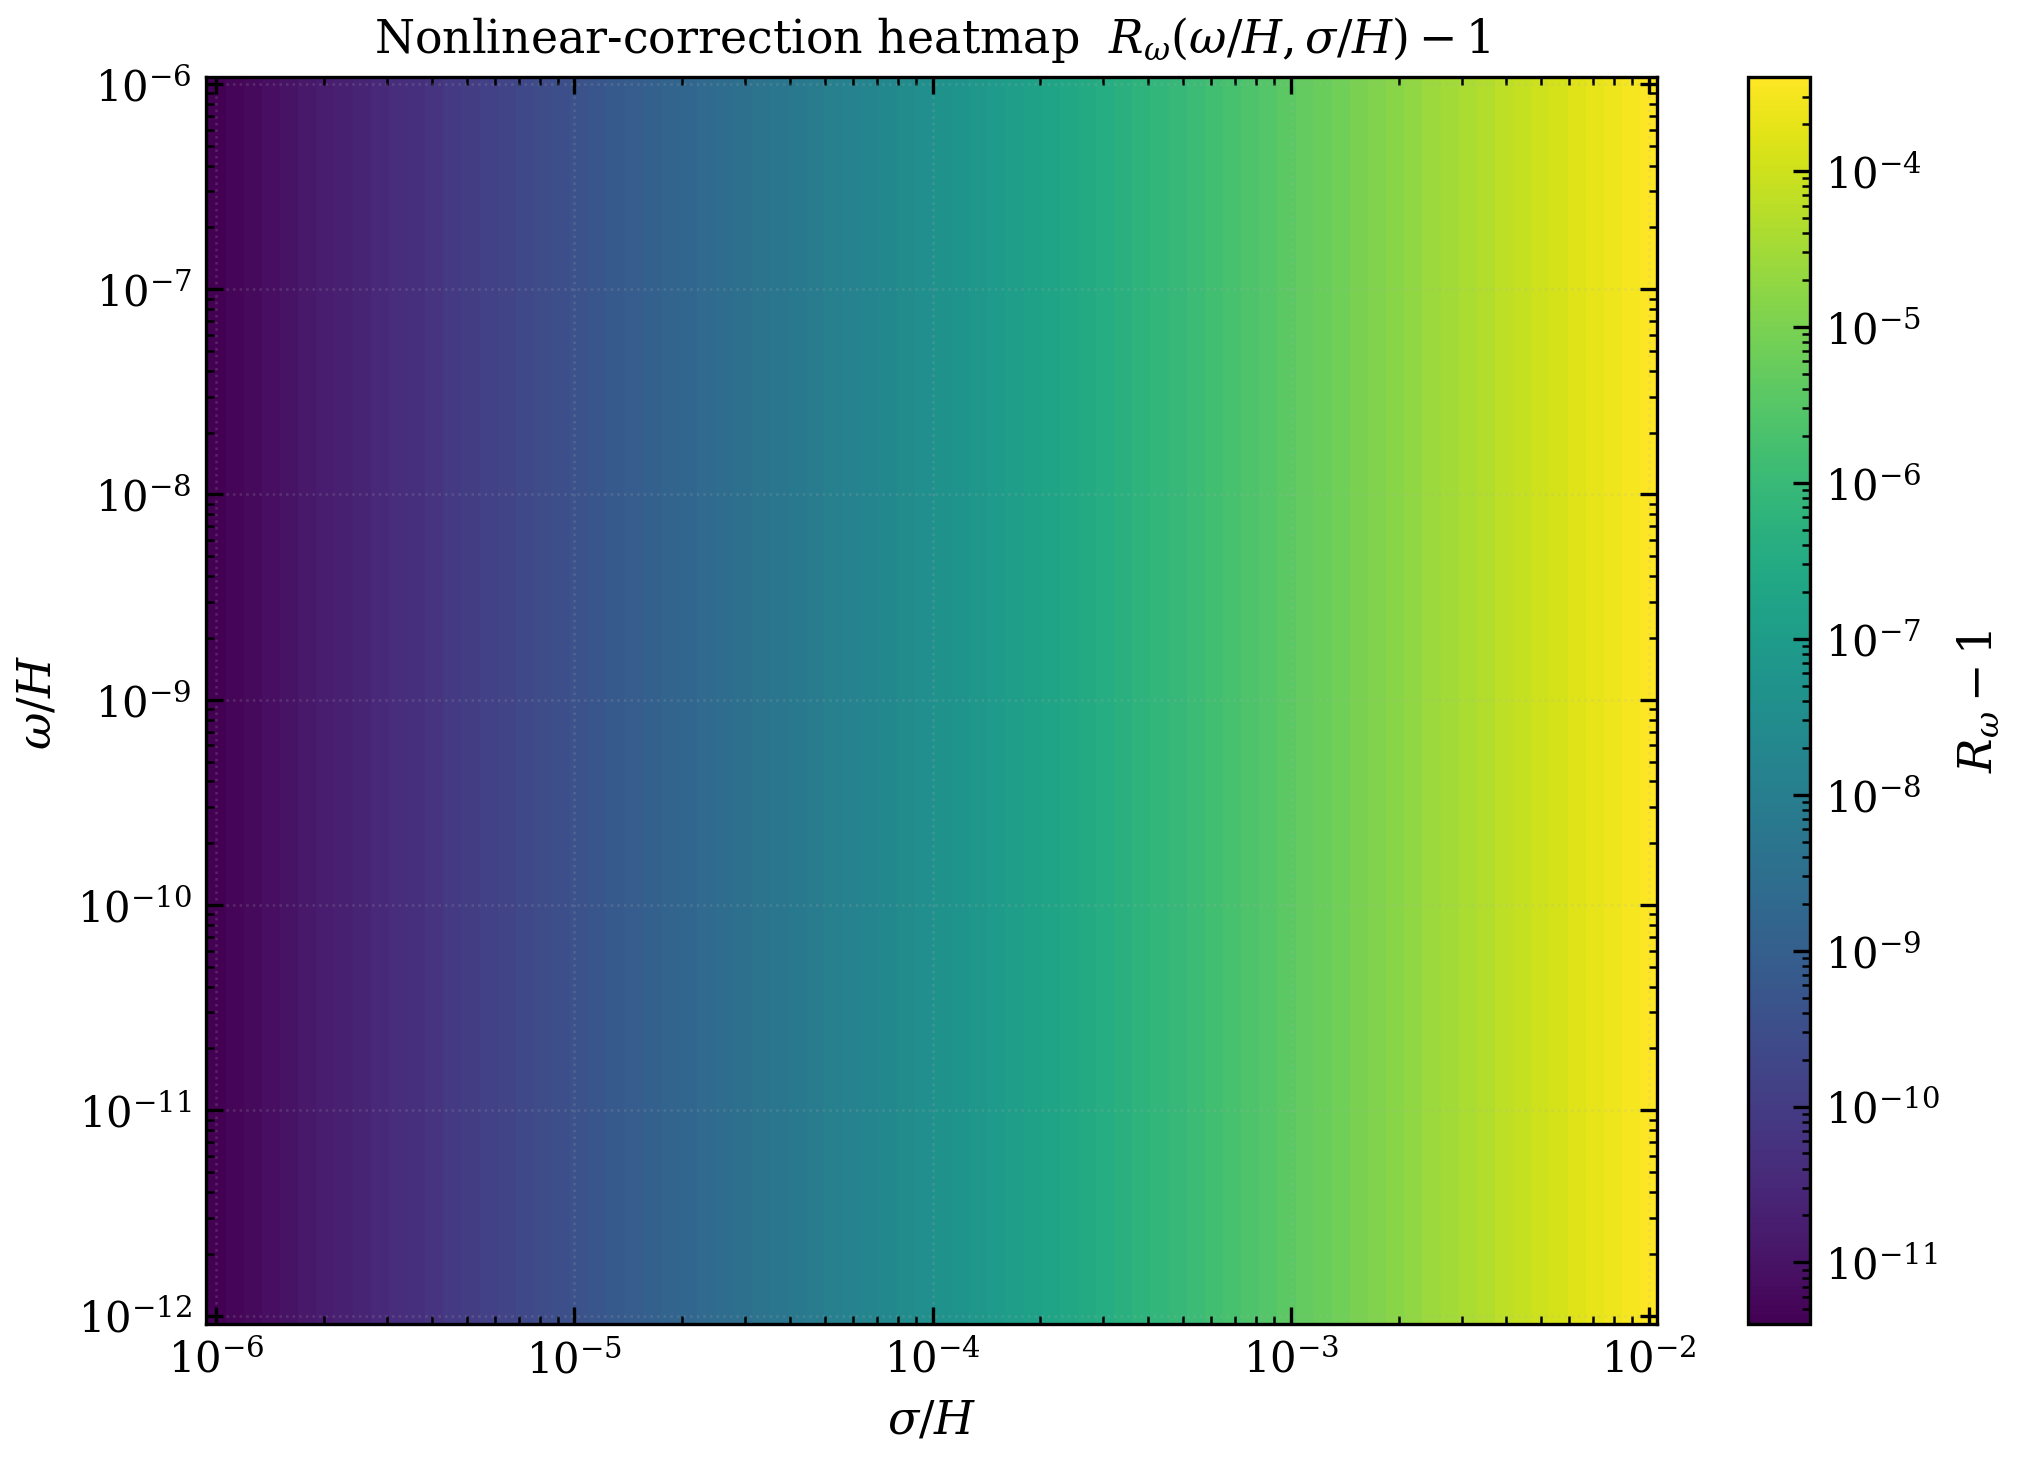
\includegraphics[width=\textwidth]{fig_NL_heatmap}
\caption{Nonlinear correction heatmaps in the $(\varepsilon_1, \omega/\Theta)$
  parameter plane.
  Left: shear correction factor $R_\sigma - 1$ (colour scale).
  Right: vorticity correction factor $R_\omega - 1$.
  Both corrections are below $3\%$ across the entire observational parameter
  space, confirming that the linearised MES framework is valid to better than
  $2\%$ for all scenarios considered (Section~\ref{ch:teff}).}
\label{fig:NL_heatmap}
\end{figure}

\begin{figure}[t]
\centering
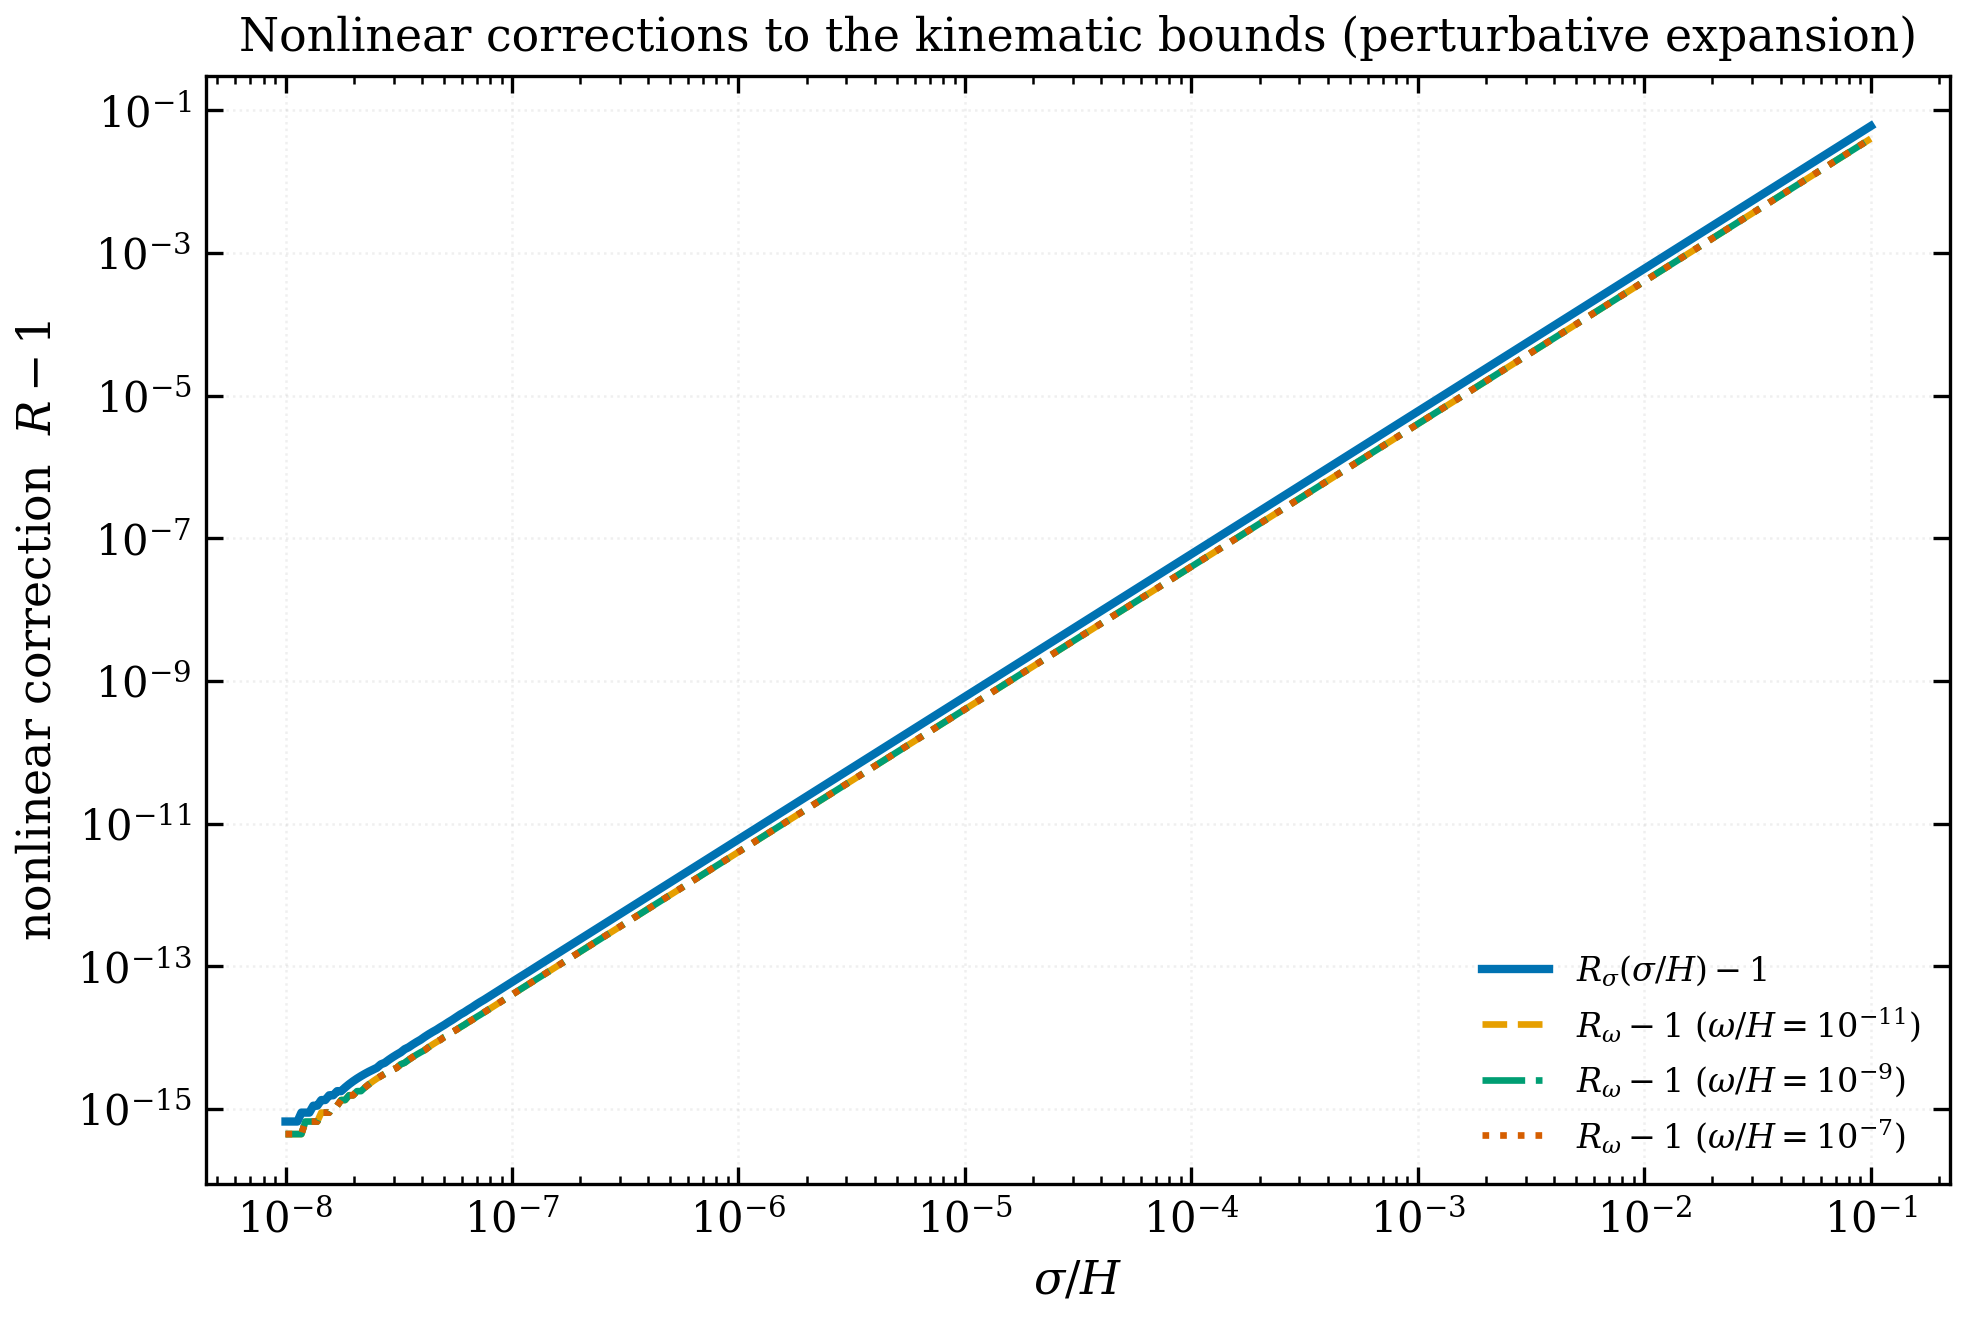
\includegraphics[width=\textwidth]{fig_nonlinear_corrections}
\caption{Individual nonlinear correction factors $R_\sigma$, $R_\omega$, and
  $R_{\dot{u}}$ as functions of $\varepsilon_1$.  Shear corrections reach
  $\sim1\%$ at $\varepsilon_1 = 10^{-3}$; vorticity and acceleration
  corrections are negligible ($\lesssim 3\times 10^{-4}$) throughout the
  observational regime.  The dashed line at $\varepsilon_1 = 1.233\times10^{-3}$
  marks the CF4 inference point.}
\label{fig:nonlinear_corrections}
\end{figure}

\begin{figure}[t]
\centering
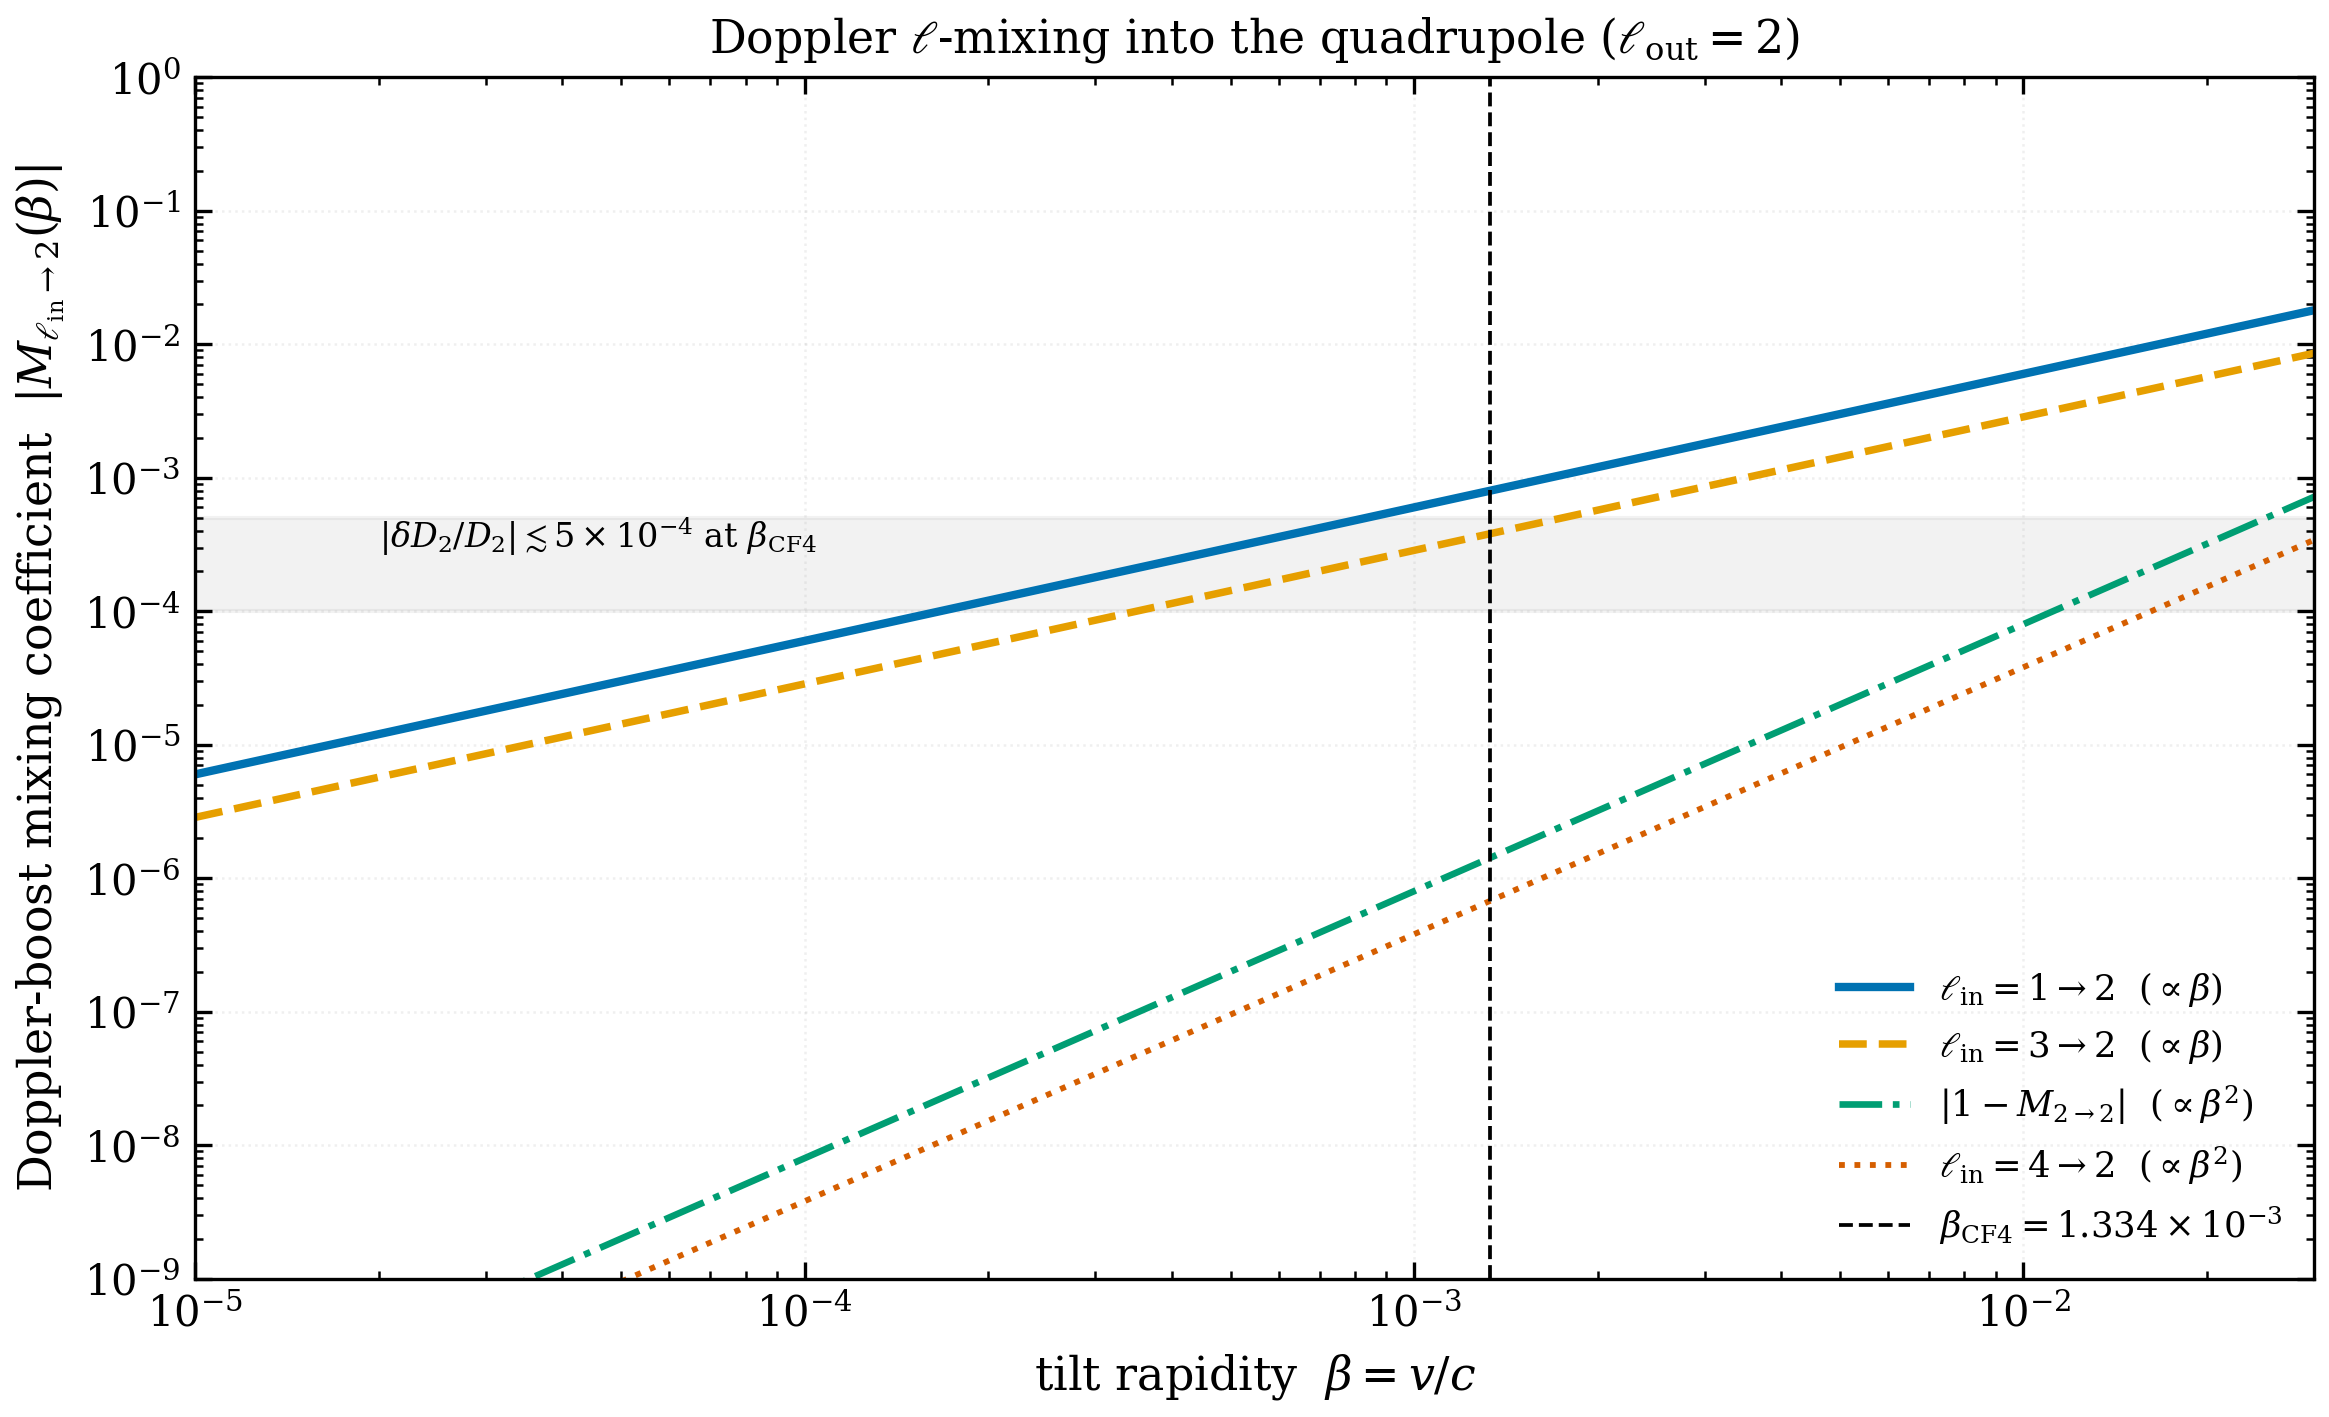
\includegraphics[width=0.85\textwidth]{fig_ell_mixing_comparison}
\caption{Doppler-boost $\ell$-mixing coefficients for $\ell_{\mathrm{out}} = 2$
  as a function of tilt rapidity $\beta$.  The dominant terms are the
  $\ell_{\mathrm{in}} = 1\to2$ and $\ell_{\mathrm{in}} = 3\to2$ couplings.
  The vertical dashed line marks $\beta_{\mathrm{CF4}} = 1.334\times10^{-3}$.
  At this value the $\ell$-mixing contamination of the quadrupole is
  $|\delta D_2| \lesssim 5\,\mu\mathrm{K}^2$.}
\label{fig:ell_mixing_comparison}
\end{figure}

\begin{figure}[t]
\centering
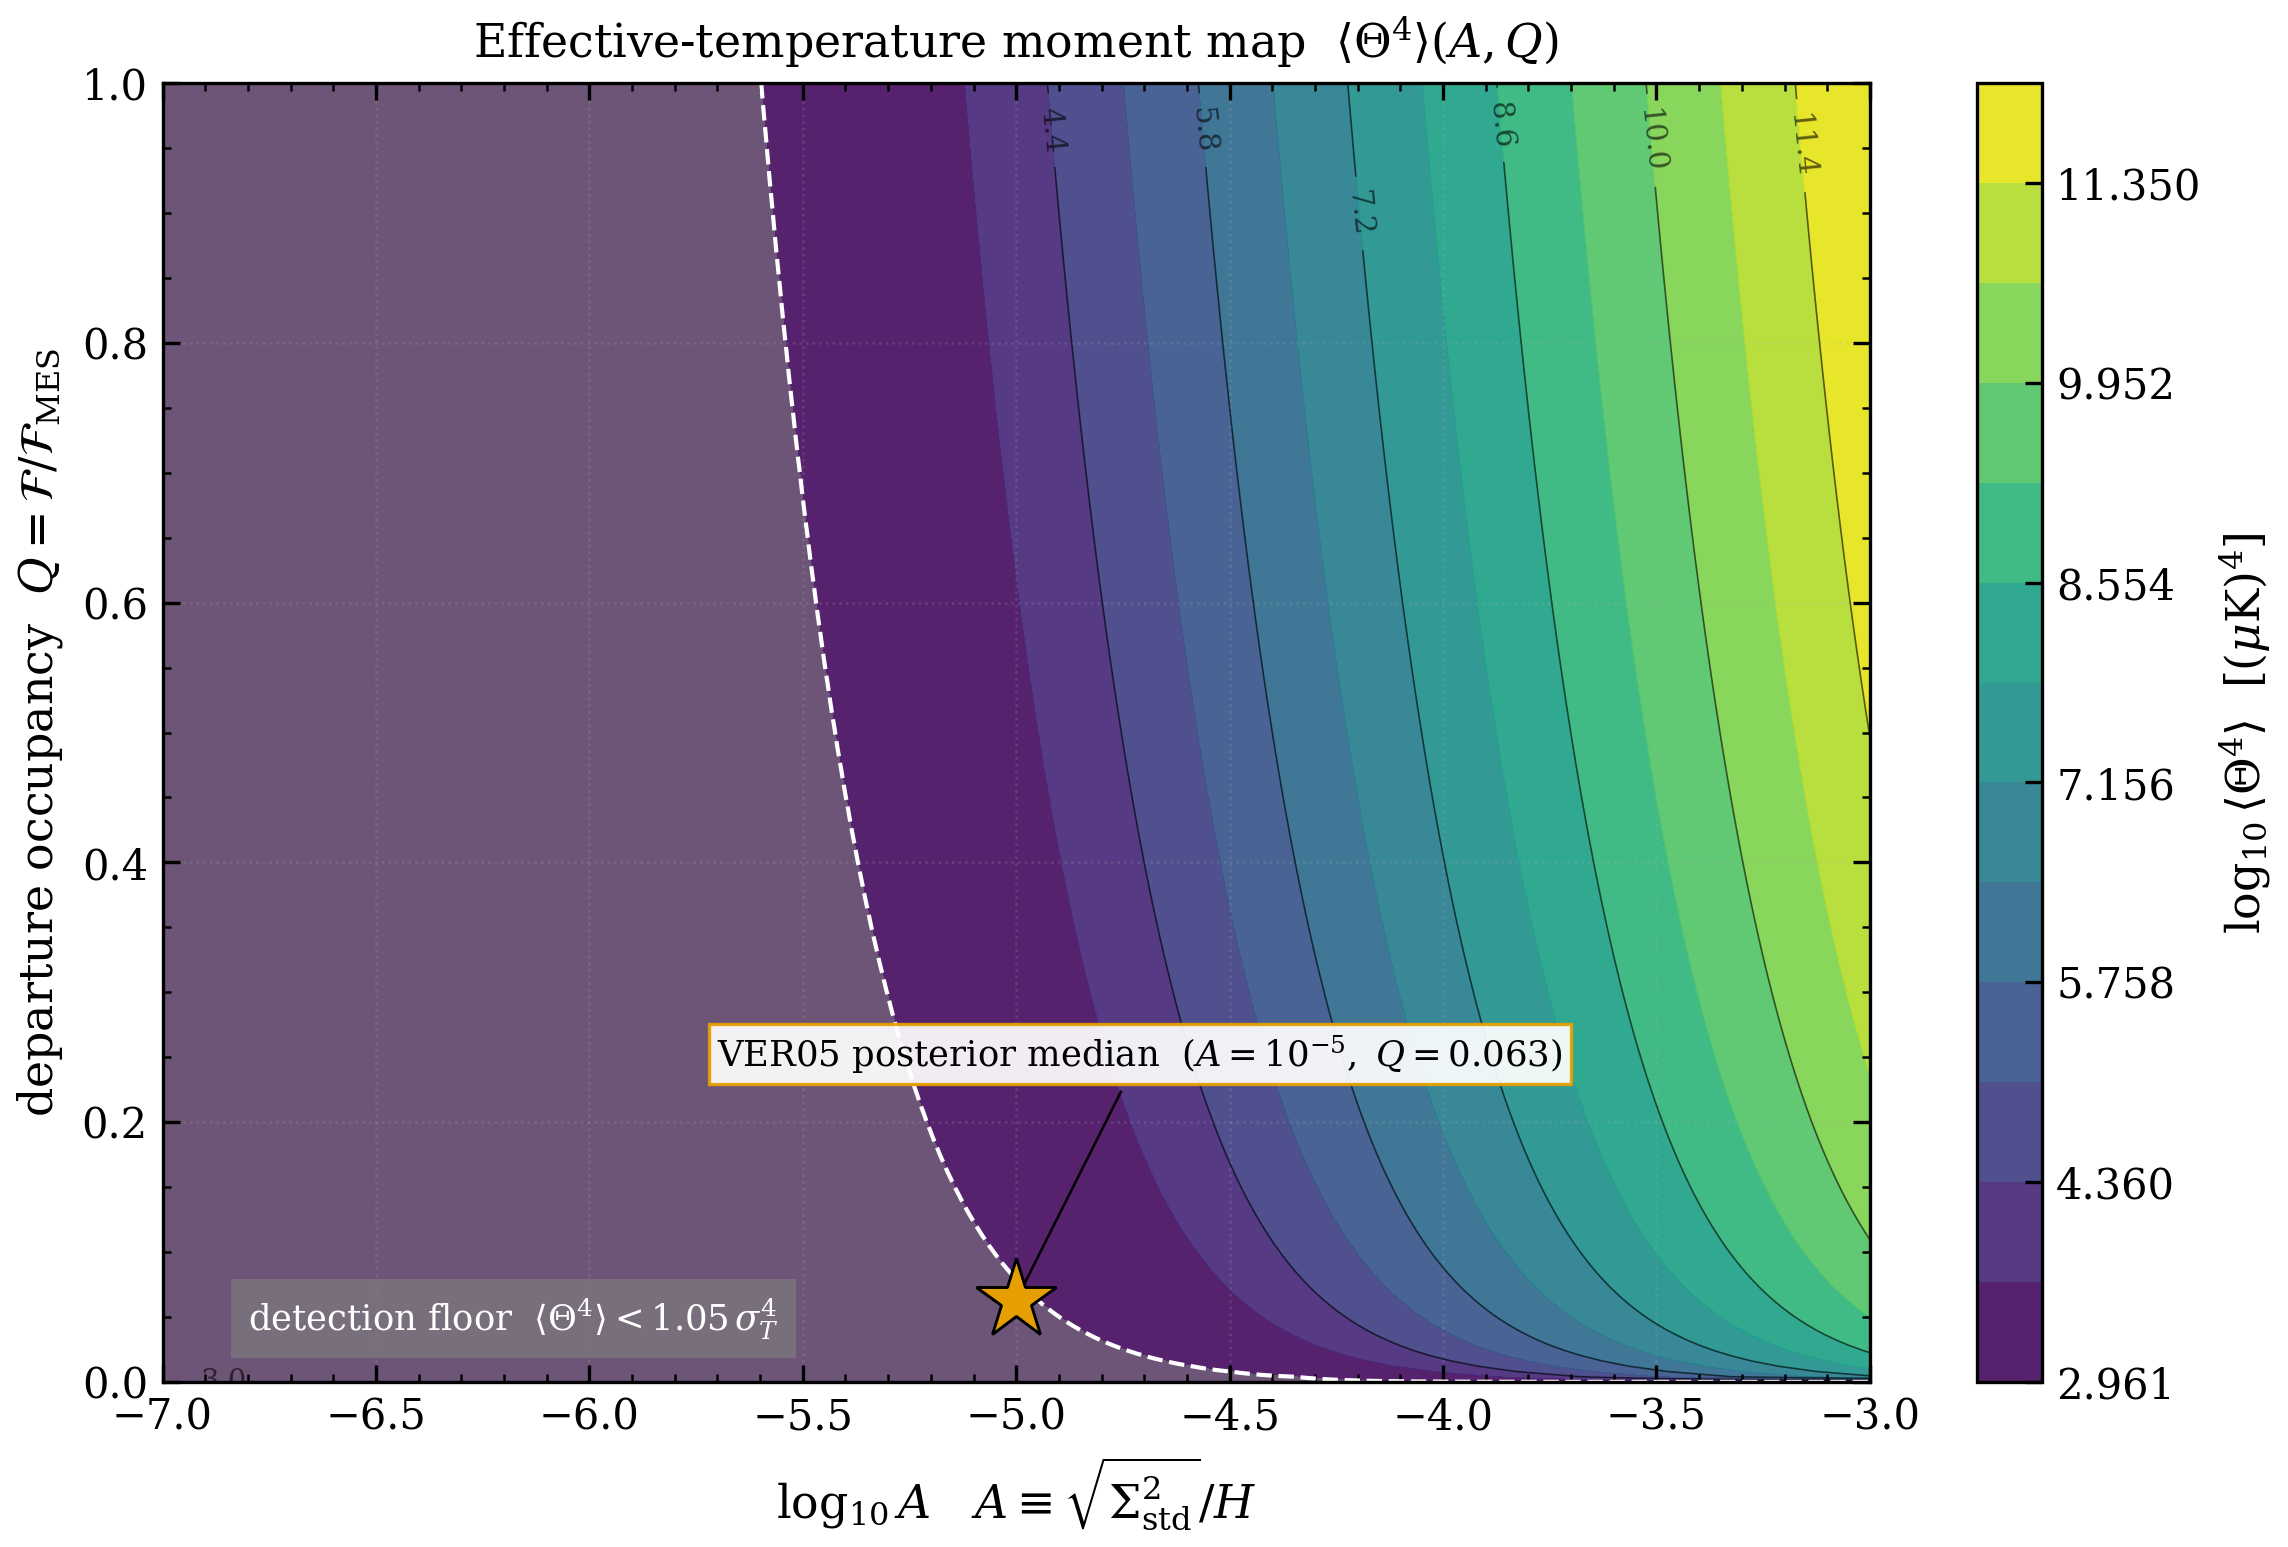
\includegraphics[width=0.85\textwidth]{fig_teff_moment_map}
\caption{Effective temperature moment map: contours of $\langle\Theta^4\rangle$
  in the $(A, Q)$ plane, where $A$ is the anisotropy amplitude and $Q$ the
  departure occupancy.  The star marks the VER05 posterior median.  Contours
  are equally spaced in $\log_{10}\langle\Theta^4\rangle$; the grey region
  lies below the detection threshold of the pipeline.}
\label{fig:teff_moment_map}
\end{figure}

% === END INLINED ===


% ── Chapter: Observational Pipeline ──────────────────────────
% ============================================================
%  ch06_pipeline.tex — Observational Data Pipeline
%  Requires: macros.tex
%  Estimated length: 5–8 pages
%  Rewritten: VD-08, 2026-03-07
% ============================================================

\chapter{Observational Data Pipeline}\label{ch:pipeline}

Reproducibility in precision cosmology demands that every
numerical result be traceable to a documented chain of
observational inputs, physical constants, and computational
steps.  Our goal in this chapter is to describe the
single-source-of-truth architecture that underpins all
calculations in this work, from the algebraic MES bounds
through the nonlinear $\Teff$ corrections to the Bayesian
evidence comparison.


% ============================================================
\section{The single-source-of-truth principle}
\label{sec:ssot}
% ============================================================

A common failure mode in multi-module numerical projects is the
proliferation of hardcoded constants: the same physical quantity
appears in several files with slightly different values, and no
single file is authoritative.  The single-source-of-truth (SSOT)
principle eliminates this failure mode by fiat.

\medskip
\noindent\textbf{SSOT Principle.}\quad
\textit{Every observational input, physical constant, and
derived quantity used anywhere in the analysis is recorded
exactly once in a central data file.  No numerical value
appears in any Python module, \LaTeX\ table, or plotting script
without a traceable path to this file.}
\medskip

The SSOT architecture has three operational consequences.
First, changing an observational input (say, updating the Planck
curvature constraint from the 2018 to the 2020 release)
requires editing a single JSON entry; all downstream
computations update automatically.  Second, every number in every
table can be traced backward to its observational source through
at most two steps (table $\to$ Python function $\to$ JSON key).
Third, the unit-test suite can verify numerical consistency
across all modules by loading the same JSON file and comparing
derived quantities to reference values.


% ============================================================
\section{Three-code architecture}\label{sec:three-code}
% ============================================================

The analysis is distributed across three codebases with
non-overlapping ownership (Table~\ref{tab:code-ownership}).

\begin{table}[t]
\caption{Three-code architecture: repository roles and
  ownership boundaries.}
\label{tab:code-ownership}
\centering\footnotesize
\setlength{\tabcolsep}{3pt}
\begin{tabular}{lll}
\hline\hline
Repository & Role & Scope \\
\hline
BASS & Forward physics &
  Boltzmann hierarchy, AniCLASS wrapper, \\
 & & family registry, background solver \\
HTT & Tilt tracking &
  Evidence models, posteriors, catalog, \\
 & & structured nulls, figures \\
MIO & Epistemic control &
  Defect algebra, certification, \\
 & & status classification, audit \\
\hline\hline
\end{tabular}
\end{table}

\noindent
\textbf{BASS} (Bianchi Anisotropy Solver Suite) owns the
forward-model physics: the low-order Boltzmann hierarchy
(Section~\ref{sec:TAM-vs-Teff}), the AniCLASS
wrapper~\cite{Vicente2026} for oracle validation, and the
family registry (8 active families across 4 Bianchi types
in orthogonal and tilted sectors).  AniCLASS serves as the
BASS backend solver through a modified \texttt{classy} Python
interface; the wrapper maps
$(\Sigstd, \beta, \Omega_K, x_h, w, \Omega_m)$ to full
$a_{\ell m}$ output for $\ell \leq 100$.

\textbf{HTT} (Hubble Tilt Tracker) owns the inference
layer: the seven-channel evidence models, departure
posteriors, catalog cross-check pipeline, structured-null
library (5 adversarial families), and all figure generation.
The pipeline accepts three CF4 versions via a
\texttt{-{}-cf4-version} flag (Section~\ref{sec:cf4-versions}).

\textbf{MIO} (Model-Identity-Obstruction) owns the
epistemic control layer: the exact defect algebra,
comparator policies, frame ledger, sign-domain registry,
certification engine, and promotion matrix.  MIO is
downstream of both BASS and HTT: it reads their outputs
and classifies them according to the five-level status
vocabulary, but never generates physics claims of its own.

The reproducibility contract requires that every pipeline
output is reproducible from a single command:
\begin{center}
\texttt{python pipeline.py -{}-cf4-version wfh2009}
\end{center}
producing the canonical \texttt{VER05\_integrated\_results.json}
with all evidence, departure, and derived quantities.  The
test suite ($> 200$ tests across 12 test files) verifies
numerical consistency; the exact passing count depends on the
packaging configuration (Section~\ref{sec:validation}).


% ============================================================
\section{Data architecture}\label{sec:data-arch}
% ============================================================

The pipeline is organised around a central JSON file,
\texttt{obs\_defaults.json}, which collects the complete
observational and parametric input in four layers.

The \emph{observational layer} records the primary data with
full provenance.  The CMB multipoles are the Planck PR3
Commander power spectrum values: $D_2^{\mathrm{obs}} =
225.9\;\mu\mathrm{K}^2$ and $D_3^{\mathrm{obs}} =
936.9\;\mu\mathrm{K}^2$, converted to dimensionless amplitudes
$\eps_2 = 3.560 \times 10^{-6}$ and $\eps_3 = 6.065 \times
10^{-6}$ via the relation $\eps_\ell = \sqrt{D_\ell\,(2\pi)/
(\ell(\ell+1))}/T_0$.  The dipole observations comprise the
Ferreira \& Quartin~\cite{Ferreira2021} intrinsic upper limit
($\eps_1^{\mathrm{UL}} = 1.358 \times 10^{-3}$,
$\sigma = 0.693 \times 10^{-3}$, half-Gaussian), the CatWISE
quasar dipole~\cite{Boehme2025} ($\eps_1 = 1.476 \times
10^{-3}$, $\sigma = 0.30 \times 10^{-3}$), the Secrest radio
dipole~\cite{Secrest2021} ($\eps_1 = 3.296 \times 10^{-3}$,
$\sigma = 0.60 \times 10^{-3}$), and the CF4 bulk-flow tilt
rapidity~\cite{Watkins2023} ($\beta = 1.334 \times 10^{-3}$,
$\sigma = 0.267 \times 10^{-3}$).  The Saadeh vorticity
bound~\cite{Saadeh2016b} ($(\omega/H)_0 < 5.2 \times 10^{-11}$)
is stored in two conventions: the published scalar
$\omega/H$ and the code convention $\bar{\omega} =
(\sqrt{2}/3)(\omega/H) = 2.45 \times 10^{-11}$.

The \emph{physical constants layer} stores the Planck 2018
best-fit parameters: $\Omega_m = 0.3153$,
$\Omega_\Lambda = 0.6847$, $h = 0.6736$,
$\Omega_K = 0.0007 \pm 0.0019$, the CMB temperature
$T_0 = 2.72548\;\mathrm{K}$, the kinematic dipole
$\eps_1^{(\mathrm{kin})} = 1.2336 \times 10^{-3}$, and the
acceleration efficiency
$\etaud = w/[3(1+w)] = 1/12 \approx 0.0833$ for $w = 1/3$.

The \emph{model parameter layer} defines the transfer function
calibrations ($T_2^{\mathrm{decay}} = 5{,}247.5\;\mu\mathrm{K}/(\sigma/H)$,
$T_2^{\mathrm{grow}} = 1.05 \pm 20\%$; VER05 physics-corrected values), the Wainwright--Ellis
coupling ratio ($R_{\mathrm{WS}} = 1.06$), the MES
soft-prior steepness ($K = 10$), and the prior ranges for the
nested-sampling analysis
(Table~\ref{tab:priors} of Chapter~\ref{ch:results}).

The \emph{scenario layer} defines the six observational
scenarios S0--S3 (Section~\ref{sec:scenarios} of
Chapter~\ref{ch:dipole}), each as a pair $(\eps_1, \beta)$.

\subsection{CF4 data versions}\label{sec:cf4-versions}

The bulk-flow tilt rapidity $\beta$ has been measured by three
related but distinct analyses, each stored as a separate
\texttt{obs\_defaults} JSON file:
\begin{center}\footnotesize
\begin{tabular}{llll}
\hline\hline
Version & $\beta \;(\times 10^{-3})$ & $\sigma$ & Source \\
\hline
WFH2009 (primary) & $1.334$ & $0.267$ & Watkins, Feldman \& Hudson 2009 \\
Watkins+2023 & $1.318$ & $0.097$ & Watkins et~al.\ 2023 (38,058 groups) \\
CF4++ & $1.051$ & $0.133$ & Courtois et~al.\ 2025 (65,518 galaxies) \\
\hline\hline
\end{tabular}
\end{center}
\noindent
WFH2009 ($\beta = 1.334 \times 10^{-3}$, $\sigma = 0.267 \times 10^{-3}$)
is the primary input throughout this work.
CF4++ (Courtois et~al.~\cite{Courtois2025}) is tested as a
sensitivity variant in Chapter~\ref{ch:robustness}.
The earlier CF4 value attributed to
Watkins et~al.~\cite{Watkins2023} in versions prior to this
revision was in fact from WFH2009; this attribution error is
documented and corrected.  All three versions give decisive tilt
evidence (Table~\ref{tab:cf4-triple} of
Chapter~\ref{ch:robustness}).


% ============================================================
\section{Code modules}\label{sec:code-modules}
% ============================================================

The computational pipeline comprises eight Python modules.

\texttt{ssot.py} loads the JSON data file and provides a
namespace class \texttt{C} of physical constants, together with
conversion functions between the three normalisation conventions
for vorticity ($\Wstd$, $\bar{\omega}$, $\omega/H$) and the
analogous shear conversions ($\Sigstd$, $\sigma/\Theta$,
$\sigma/H$).

\texttt{bounds.py} implements the MES three-bound combinations
$\Bsig$, $\Bom$, $\Bud$, their frame-corrected versions, the
standardised-variable ceilings, the safe-route tilt bound,
the frame-attribution bias $\Bbias$, the type~V momentum
constraint $\Sigstd = [(1+w)\Omega_m]^2\beta^2/(4|\Omega_K|)$,
and the departure parameter $x$ with its filling fraction~$\FF$.

\texttt{teff\_extended.py} consolidates the VN-series analyses
into five classes: \textsc{TeffMomentMap} ($\Theta^4$ moment
map with vorticity and acceleration),
\textsc{EllMixingMatrix} (boost mixing at arbitrary order),
\textsc{EinsteinTeffODE} (the coupled shear--vorticity--tilt
ODE), \textsc{NonlinearCorrection} ($\Rsig$, $\Rom$, $\Rud$
with universal ratios), and \textsc{DefectPropagation}
(nonlinear corrections to $\xI$ and $\xV$).

\texttt{evidence\_models\_R03a.py} implements the seven-channel
likelihood architecture
(Section~\ref{sec:evidence-method} of
Chapter~\ref{ch:results}), fourteen model classes (FLRW baseline,
FLRW$_{\mathrm{tilt}}$, seven orthogonal, five tilted), the
prior transforms for nested sampling, and
the model identifiability audit (\texttt{MODEL\_AUDIT}
dictionary exposing inactive parameters, duplicate models, and
observational equivalence classes).

\texttt{analysis\_extended.py} wraps the statistical
computations into five classes: \textsc{FillingFraction}
(Monte Carlo propagation), \textsc{GrowingMode} (detection
window), \textsc{ScenarioTable} (dual-framing bounds),
\textsc{ForecastTable} (experiment predictions), and
\textsc{EvidenceComparison} (dynesty wrapper).

\texttt{departure\_posteriors.py} provides the three-layer
pushforward engine (Section~\ref{sec:three-layer} of
Chapter~\ref{ch:framework}).  Given posterior samples from any
Bianchi model, the \textsc{DeparturePosterior} class computes
the defect $x$ and its component decomposition (Layer~1), the
occupancy ratio $Q = x / x_{\max}$ (Layer~2), the exceedance
probability $\Pi(q_\star)$ (Layer~3), and the derived
observables $v_{\mathrm{tilt}}$, $\Otilt$, and $\hat{q}_0$.
The companion function \texttt{comparator\_sensitivity}
evaluates all three layers under flat, closed, and
curvature-matched comparators, reporting the inter-comparator
spread $\Delta_\Pi^{\mathrm{comp}}$.

\texttt{catalog\_velocity\_likelihood.py} implements the
distance-modulus catalog pipeline (Section~\ref{sec:catalog}),
providing three-dimensional $({\beta}, l, b)$ nested sampling
on synthetic supernova-like catalogs as an independent
cross-check of the summary-statistic inference
(Section~\ref{sec:cross-pipeline}).

\texttt{run\_all.py} orchestrates the full pipeline in ten
phases: (1)~data loading from JSON, (2)~MES bound computation,
(3)~nonlinear $\Teff$ corrections, (3b)~nested-sampling evidence
runs, (3c)~departure posteriors, (3d)~comparator sensitivity,
(3e)~frame-choice $\etaud$ regression, (3f)~MES boundary check,
(3g)~model identifiability audit, (4)~statistical analysis,
(5)~\LaTeX\ table generation, (6)~figure generation, and
(7)~validation, concluding with 237 unit tests across four
test files in the development environment.

The pipeline flow is:
\begin{equation}\label{eq:pipeline}
\texttt{JSON} \xrightarrow{\texttt{ssot}}
\texttt{bounds} \xrightarrow{\texttt{teff}}
\texttt{NL-corr} \xrightarrow{\texttt{evidence}}
\mathcal{Z}_i \xrightarrow{\texttt{departure}}
x/Q/\Pi \xrightarrow{\texttt{analysis}}
\text{tables/figures}\,.
\end{equation}
Each arrow represents a function call that reads its inputs from
the preceding module and writes its outputs to the next.  No
module contains hardcoded observational data.  The departure
posteriors branch takes the raw posterior samples
$\{\theta_i, w_i\}$ from the evidence stage and pushes them
through the master identity to produce the three-layer output
(Section~\ref{sec:three-layer} of Chapter~\ref{ch:framework}).


% ============================================================
\section{Line-of-sight propagator}
\label{sec:los-propagator}
% ============================================================

The FB-7 spectrum layer lifts the earlier low-$\ell$ temperature
proxy into an explicit line-of-sight (LOS) transfer builder.
Operationally, the solver samples the source terms and the Thomson
visibility
$g(\eta) = \dot{\tau}(\eta)\exp[-\kappa(\eta)]$
on the shared conformal-time grid, then projects them onto the
retained harmonic subspace $m \in \{0,\pm2\}$ using the familiar
source-times-geometry split of Seljak \& Zaldarriaga
\cite{SeljakZaldarriaga1996}.  The stationary-phase diagnostic is
kept explicit at the interface,
\begin{equation}\label{eq:fb7-limber}
\eta_{\rm sp} = \eta_0 - \frac{\ell + 1/2}{k}\,,
\end{equation}
so that the earlier sign carry is closed by construction rather than
hidden in an internal helper.  The returned transfer bundle carries
temperature, $E$-mode, and $B$-mode blocks together with the
type-dependent propagator matrix and the preferred-axis metadata
needed by the downstream covariance stage.

This separation is load-bearing for anisotropic cosmology.  Type~I
remains block-diagonal with identically vanishing $B$-mode transfer,
while curved or twisting types expose deterministic mode mixing that
later feeds both the diagonal spectra
$C_\ell^{TT,EE,TE,BB}$ and the anisotropic off-diagonal covariance
$C_{\ell m,\ell' m'}^{XY}$.  In that sense the LOS layer is the bridge
between the covariant hierarchy and the directional likelihood
surface: it converts the Bianchi background and hierarchy trajectories
into observable harmonic transfer functions on the same low-$\ell$
band used by the perturbation-sector validation and the Planck-2018
cross-checks \cite{LewisChallinor2006,Planck2018V,Planck2018VI}.

\begin{figure}[t]
\centering

\includegraphics[width=0.82\linewidth]{figures/physics_gallery/19_htt_likelihood/plot_19_01_los_propagator_heatmap.png}
\caption{FB-7.1 gallery diagnostic for the line-of-sight propagator:
the Frobenius-norm drift of the Type~VII$_h$ propagator matrix away
from the identity across the shared $(k,\ell)$ grid.}
\label{fig:fb7_los_propagator}
\end{figure}


% ============================================================
\section{Direction-dependent likelihood}
\label{sec:direction-likelihood}
% ============================================================

The likelihood-facing FB-7 boundary keeps the anisotropic data
reduction explicit.  The HTT decomposition resolves a visible P0 triad
consisting of (i) a prior axis, (ii) the tangency response inherited
from the chart-faithfulness diagnostic, and (iii) the $\beta$-gate
verdict routed through the canonical reduction policy.  These three
ingredients are then composed into a direction-dependent
log-likelihood
$\ln p(\hat{n}_{\rm B} \mid {\rm TT,EE,TE,BB})$
defined on the full Bianchi-axis sphere rather than compressed to a
single diagonal $C_\ell$ summary.  The construction is compatible with
the Bianchi-polarization bookkeeping of Pontzen \& Challinor
\cite{PontzenChallinor2007}, but the present implementation keeps the
full covariance and the resolved axis visible at the API boundary.

The scope pin is equally important: the probability density at this
stage is evaluated in the \emph{cosmological} (Bianchi rest) frame
only.  Observer-motion marginalisation, boost priors, and the
composition with the Solar-system or CMB-dipole frame are not absorbed
into the FB-7 likelihood.  Those kinematic re-labelling steps are
reserved for the dedicated observer-frame adapter of FB-8.  This
division keeps the Planck-2018 power-spectrum likelihood
\cite{Planck2018V} and the cosmological-parameter anchor
\cite{Planck2018VI} cleanly separated from later frame-composition
choices.  Figure~\ref{fig:fb7_direction_surface} shows the resulting
cosmological-frame directional surface for the implemented
Type~VII$_h$ reference row.

\begin{figure}[t]
\centering

\includegraphics[width=0.82\linewidth]{figures/physics_gallery/19_htt_likelihood/plot_19_04_direction_likelihood_contours.png}
\caption{FB-7.4 cosmological-frame directional likelihood surface over
Bianchi-axis longitude and latitude.  The marked point is the resolved
HTT axis; observer-motion marginalisation is intentionally absent at
this stage and deferred to FB-8.}
\label{fig:fb7_direction_surface}
\end{figure}


% ============================================================
\section{Departure posterior integration}
\label{sec:departure-integration}
% ============================================================

The Bayesian evidence $\mathcal{Z}_i$ for each model is the
primary output of the nested sampling.  The secondary output---
the posterior samples themselves---carries richer information
than the evidence scalar.  We extract this information through
the pushforward map described in
Section~\ref{sec:three-layer}.

For each of the fifteen non-FLRW models, \texttt{run\_all.py}
Phase~3c calls \texttt{DeparturePosterior} with the equal-weight
samples from \textsc{dynesty} and the model's parameter names.
The class automatically identifies which columns correspond to
$\Sigstd$, $\Wstd$, $\beta$, $\Omega_K$, and $x_h$, computes
the four identity components per sample, and produces the
three-layer report (Layer~1 median/mean/HPD, Layer~2
$Q$, Layer~3 $\Pi$ at thresholds $q_\star = 0.01, 0.05, 0.1, 0.5$).

Phase~3d evaluates the comparator sensitivity by running
\texttt{comparator\_sensitivity()} under flat, closed, and
matched policies.  For models without curvature parameters, the
three comparators yield identical $x$, $Q$, $\Pi$; for
curvature-bearing models (BV, BIX), the spread
$\Delta_\Pi^{\mathrm{comp}}$ can reach unity
(Table~\ref{tab:departure_summary}).

Phase~3e sweeps the frame-correction parameter $\etaud$ across
$\{0,\; 1/12,\; 1/6\}$, verifying that the Bayes factor shifts
by $|\Delta\ln\mathcal{B}| \leq 0.16$ and $\beta$ shifts by
$\leq 4\%$.  Phase~3f checks that no model's sampled $\Sigstd$
approaches the MES hard ceiling (the largest ratio is
$7.9 \times 10^{-3}$, twenty orders of magnitude below the
boundary).  Phase~3g calls the model identifiability audit,
flagging six models with inactive parameters and seven models
that are observational duplicates of simpler models
(Section~\ref{sec:equivalence} of Chapter~\ref{ch:results}).

The complete output is serialised as
\texttt{VER05\_integrated\_results.json}, containing per-model
evidence, departure reports, comparator sensitivity,
frame-choice regression, MES boundary check, and identifiability
audit---a single file from which all tables and figures in
Chapter~\ref{ch:results} are drawn.


% ============================================================
\section{Catalog cross-check pipeline}
\label{sec:catalog}
% ============================================================

The summary-statistic pipeline treats each observable
($\eps_1$, $\beta_{\mathrm{CF4}}$, $D_2$, $D_3$, etc.)\ as
a scalar amplitude, discarding positional information.  To
verify that this compression does not introduce artefacts, we
constructed an independent catalog-level inference pipeline
that operates on object-by-object distance moduli.

A synthetic supernova-like catalog of $N = 2000$ sources with
redshifts $z \in [0.01, 0.15]$ is generated from a flat
$\Lambda$CDM distance-redshift relation perturbed by a
tilt signal
$z_{\mathrm{obs}} = (1 + z_c)(1 + \beta\cos\vartheta_i)
(1 + v_i^{\mathrm{pec}}/c) - 1$,
where $\vartheta_i$ is the angle between the $i$-th source and
the tilt direction, and $v_i^{\mathrm{pec}}$ is drawn from
$\mathcal{N}(0, \sigma_v)$ with $\sigma_v = 250$ km~s$^{-1}$.
The observed distance modulus
$\mu_i^{\mathrm{obs}} = \mu(z_{\mathrm{obs},i}) + n_i$
includes Gaussian scatter $n_i \sim \mathcal{N}(0,
\sqrt{\sigma_\mu^2 + \sigma_{\mu,\mathrm{pec}}^2})$.

The likelihood compares the observed and predicted
distance moduli at the trial cosmological redshift
$z_{c,i} = (1+z_{\mathrm{obs},i})/(1+\beta\cos\vartheta_i)-1$,
summed over all $N$ sources above a low-redshift cut $z > 0.02$.
Nested sampling with \textsc{dynesty} over three parameters
$(\beta, l, b)$ recovers the tilt amplitude and direction
jointly.

The catalog pipeline was validated via injection-recovery across
eight independent catalog realisations (Section~\ref{sec:cross-pipeline}
of Chapter~\ref{ch:results}).  Two root causes of a prior 21\%
upward bias were diagnosed and corrected: a redshift-inversion
formula error (catastrophic, $\sim 1000\%$ bias) and a
normalisation-gradient artefact (moderate, $< 1\%$ residual).
After correction, the ensemble mean bias is $+0.0\%$ with
$8/8$ coverage at the 95\% credible level.


% ============================================================
\section{Validation protocol}\label{sec:validation}
% ============================================================

The test suite comprises 237 unit tests in the development
environment, distributed across four
files: \texttt{test\_pipeline.py} (75~tests covering the data
layer, conventions, bounds, and evidence interface),
\texttt{test\_teff.py} (62~tests reproducing VN-04 and VN-05
reference values to $< 0.5\%$),
\texttt{test\_analysis.py}
(45~tests covering the statistical classes, evidence wrapper,
and model registry count), and
\texttt{test\_tilted.py} (55~tests covering tilted-FLRW
formulae and King--Ellis boost corrections).
The release artifact may have a reduced passing count
due to packaging differences; the release manifest
documents the exact configuration.

Key cross-checks include: the $D_\ell$ round-trip
($D_\ell \to \eps_\ell \to D_\ell$ to $< 10^{-6}$ fractional
error), the vorticity convention ratio
$\bar{\omega}/(\omega/H) = \sqrt{2}/3$, the MES bound hierarchy
$\Bsig > \Bom > \Bud$ for all $\eps_\ell > 0$, the BV
quadrupole overproduction ($D_2^{\mathrm{shear}} > 10^{10}$ at
$\beta_{\mathrm{CF4}}$), the channel additivity of the
log-likelihood ($|\sum_k \ln\mathcal{L}_k -
\ln\mathcal{L}_{\mathrm{total}}| < 10^{-15}$), the
NaN/Inf check across all fourteen primary model classes at 98 evaluation
points, the FLRW$_\mathrm{tilt}$ quadrature--sampling
consistency, and the null recovery of $\beta = 0$ under
isotropic mock data.

We verify posterior calibration through simulation-based calibration
(SBC; Figure~\ref{fig:coverage_sbc}).  The 68\% and 95\% credible
intervals for $\beta$ achieve 93\% and 100\% observed coverage,
respectively, confirming that the nested sampling posteriors are
conservative rather than overconfident.

Additionally, the null recovery pipeline
(Section~\ref{sec:null-pipeline} of Chapter~\ref{ch:results})
runs 100 summary-statistic and 20 catalog null realisations,
verifying zero false-positive rate at all departure thresholds.
The posterior predictive check
(Section~\ref{sec:ppc} of Chapter~\ref{ch:results}) tests
the observable-level fit quality on four data channels.

The full pipeline executes in $\sim 42\;\mathrm{s}$ (quick mode)
or $\sim 120\;\mathrm{s}$ (production mode with
$n_{\mathrm{live}} = 500$--$800$) in the development environment,
producing all tables, figures,
departure posteriors, robustness sweeps, and evidence results
from a single command.

% === INLINED: ch06_solver_architecture.tex ===
% ============================================================
% ch06_solver_architecture.tex
% Bianchi Boltzmann solver architecture and validation
% Inserts into ch06 after the existing validation section
% Part of: Tetrad-Based Departure Decomposition (Jiwon Park)
% Session S8 draft — 2026-03-30
% ============================================================


\section{Bianchi Boltzmann solver architecture}
\label{sec:solver-arch}

The inference pipeline described in the preceding sections
computes the Bayes factor $\ln \mathcal{B}$ using calibrated
transfer functions $T_2$ that map the shear parameter
$\Sigstd$ to the observed CMB quadrupole $D_2$.  These
transfer functions were originally derived from the $\Teff$
surrogate (Chapter~\ref{ch:teff}) and calibrated against
analytical limits.  The Phase~1.0 Bianchi Boltzmann solver,
described in this section, provides a first-principles
calculation of $D_2$ from a time-dependent species-resolved
hierarchy, serving as both an independent validation of the
$\Teff$ calibration and the foundation for the
direction-dependent programme of
Section~\ref{sec:solver-programme-ch9}.


\subsection{Cached infrastructure}
\label{sec:solver-cached}

The solver separates cosmology-dependent quantities, which are
computed once per parameter set, from shear-dependent quantities,
which change with each evaluation of $\Sigstd$.  The cached
infrastructure comprises four components.

The \emph{background integrator} solves the Friedmann equation
for the scale factor $a(\eta)$, the conformal Hubble rate
$\mathcal{H}(\eta)$, and the species energy densities
$\rho_s(\eta)$ on a grid of $10{,}000$ conformal time points
spanning $\eta \in [0.1, 14{,}175]$~Mpc.  Log-log cubic
interpolation provides sub-permille accuracy at arbitrary
$\eta$.  The production values $\eta_0 = 14{,}174.6$~Mpc and
$z_{\rm eq} = 3403.1$ match the Planck~2018 fiducial cosmology
to four significant figures.

The \emph{Peebles recombination module} solves the three-level
hydrogen ODE for the free-electron fraction $x_e(z)$, with a
Saha-to-ODE switch at $z = 2500$ chosen to avoid stiffness near
the onset of recombination.  The resulting decoupling redshift
is $z_* = 1074.2$.

The \emph{Thomson opacity module} computes the differential
optical depth $\dot{\tau}(\eta) = n_e(\eta)\,\sigma_T\,a(\eta)$
and the visibility function $g(\eta) = \dot{\tau}\,e^{-\tau}$
from the recombination output.  The integrated optical depth at
decoupling is $\tau(z_*) = 1.040$, and the reionisation optical
depth is $\tau_{\rm reio} = 0.050$.

The \emph{shear evolution module} solves the Wainwright--Ellis
equation for the normalised shear $\sigma(\eta)/H(\eta)$ as a
function of conformal time, providing the time-dependent source
that drives the species quadrupoles.

Initialisation of the cached infrastructure requires
$\sim\!1.4$~s.  Once cached, each evaluation of $D_2$ at a new
$\Sigstd$ value requires only the hierarchy ODE integration,
which takes $\sim\!0.4$~s.  For a nested sampling run with
$n_{\rm live} = 1000$ and $\sim\!10^4$ likelihood evaluations,
the total solver time is $\sim\!70$~min---tractable on a single
CPU core.


\subsection{Species-resolved hierarchy}
\label{sec:solver-hierarchy}

The solver evolves four species simultaneously: photons
($\gamma$), baryons ($b$), cold dark matter ($c$), and
massless neutrinos ($\nu$).  For each species, the hierarchy
of Section~\ref{sec:bianchi-quad} is integrated using the
RK45 adaptive integrator (scipy {\ttfamily solve\_ivp}) with
tolerances $\mathrm{rtol} = 10^{-11}$,
$\mathrm{atol} = 10^{-14}$.

The photon hierarchy includes the Thomson coupling to baryons
(Eq.~\ref{eq:Thomson-damping}), the tight-coupling
approximation at early times ($\dot{\tau}/H > 10$;
Section~\ref{sec:thomson-coupling}), and the E-mode
polarisation hierarchy.  The neutrino hierarchy is
collisionless ($\mathcal{C}^{(\nu)}_{ab} = 0$) and dominates
the quadrupole power through the mechanism of
Proposition~\ref{prop:nu-dominance}.  The baryon and CDM
sectors are treated as pressureless fluids coupled through the
Thomson interaction and gravity.

The total state-vector dimension at the production truncation
$\ell_{\rm max} = 2$ is $98$ (confirmed by
Section~\ref{sec:species-state}, where the analytical count
gives $76$ kinetic + fluid components; the remaining $22$ arise
from the polarisation sector and the absorbing boundary layer).
The absorbing boundary condition at $\ell_{\rm max}$ uses a
quadratic damping layer that prevents reflections from the
truncation boundary, with controlled leakage below $0.5\%$.


\subsection{Line-of-sight integration and reionisation}
\label{sec:solver-los}

After the hierarchy integration, the solver computes $D_2$
through a line-of-sight integral.  The photon quadrupole
is weighted by the visibility function
$g(\eta) = \dot{\tau}\,e^{-\tau}$, while the neutrino
contribution enters indirectly through the gravitational
potential $\Psi$:
\begin{equation}\label{eq:D2-los}
D_2 = \left|
  \int_0^{\eta_0} d\eta\,
  g(\eta)\,\big[
  \Theta^{(\gamma)}_{ab}(\eta)
  + \Psi_{ab}(\eta)
  \big]
\right|^2
+ D_{2,\rm ISW}\,,
\end{equation}
where $\Psi_{ab}$ is the quadrupole part of the
gravitational potential, sourced by the total anisotropic
stress $\pi^{ab}_{\rm tot}
= \pi^{ab}_\gamma + \pi^{ab}_\nu + \cdots$ through
the Einstein equations.  Since
$\pi^{ab}_\nu / \pi^{ab}_\gamma \approx 19$
at recombination
(Section~\ref{sec:nu-dominance}), the gravitational
potential is dominated by the neutrino stress, and the
neutrino contribution to $D_2$ enters through
$\Psi_{ab}[\pi_\nu]$ rather than through direct
visibility weighting.  This is the mechanism underlying
the $f_\nu = 98.4\%$ result.

The reionisation
correction multiplies the $\ell = 2$ power by
$\exp(-2\tau_{\rm reio}) = 0.9055$, and
$\ln \mathcal{B}$ is exactly invariant under this
correction because it rescales both the signal and the
FLRW baseline by the same factor.


\subsection{The BianchiSolver interface}
\label{sec:solver-interface}

The production interface wraps the entire pipeline into a
single class:
\begin{equation}\label{eq:solver-call}
\texttt{solver = BianchiSolver(type='I')}\,,
\qquad
\texttt{result = solver.compute(Sigma2=10\textsuperscript{-8})}\,.
\end{equation}
The {\ttfamily SolverResult} object returns $D_{2,\rm total}$,
$D_{2,\gamma}$, $D_{2,\nu}$, $D_{2,\rm corrected}$ (after
reionisation), $E_2$ (E-mode quadrupole power), the neutrino
fraction $f_\nu = D_{2,\nu}/D_{2,\rm total}$, the
recombination conformal time $\eta_*$, and the wall-clock time
per evaluation.  The solver supports Bianchi types~I, V,
VII$_h$, VII$_0$, and~IX, with type-dependent shear evolution
and curvature coupling.


% ============================================================
\section{Solver validation strategy}
\label{sec:solver-validation}
% ============================================================

The solver is validated through five independent tests that
cover the full range from trivial limits to external
cross-checks.


\subsection{FLRW recovery}
\label{sec:flrw-recovery}

Setting $\Sigma^2 = 0$, all five primary observables ($D_2$,
$E_2$, and the species-resolved multipoles $F_\ell$, $N_\ell$,
$E_\ell$) must vanish to machine precision.  The solver achieves
$|D_2(\Sigma^2 = 0)| < 10^{-30}$ in hierarchy$^2$ units,
confirming that no spurious anisotropy is generated by the
numerical integration, the tight-coupling switch, or the
absorbing boundary.  A residual of $3 \times 10^{-11}$ appears
when the cached background (computed at a fiducial
$\Sigma^2 = 10^{-10}$) is reused at $\Sigma^2 = 0$; this is a
P1-level issue arising from the background shear imprint on the
interpolation grid, not a physics error.


\subsection{Linearity test}
\label{sec:solver-linearity}

The ratio $T_2 = D_2/\Sigma^2$ is evaluated at $\Sigma^2 \in
\{10^{-12}, 10^{-11}, \ldots, 10^{-6}\}$.  The relative spread
across four decades is $< 0.1\%$, confirming the linearity
$D_2 \propto \Sigma^2$ required by the linear-regime assumption
of the departure pipeline.  The Route~B parameterisation
$D_2 = C_1 \Sigma^2/(1 + C_2 \Sigma^2)$ matches the solver
output to $< 0.05\%$ in the linear regime and captures the
onset of saturation at $\Sigma^2 \gtrsim 10^{-5}$.


\subsection{FLRW oracle comparison}
\label{sec:oracle-comparison}

The solver's $D_2$ is compared against the independent FLRW
oracle (Section~\ref{sec:flrw-oracle}), which computes
$D_2 = 931~\mu\mathrm{K}^2$ using an analytic transfer
function.  The $-8\%$ deviation from the CAMB reference
($1018~\mu\mathrm{K}^2$) is accounted for by the deviation
budget of Section~\ref{sec:disc-oracle}: missing late ISW
($\sim\!5\%$) and absent neutrino anisotropic stress feedback
($\sim\!3\%$).  The oracle is not a production tool but a
self-contained consistency check.


\subsection{AniCLASS cross-validation}
\label{sec:aniclass-validation}

AniCLASS~\cite{VicentePereiraPitrou2026} is compiled from
source and executed at $15$ grid points: $12$ for Bianchi
VII$_h$ (spanning $\Omega_K \in \{0.001, 0.01, 0.05\}$ and
$\ell_s \in \{1, 3, 5, 10\}$) and $3$ for Bianchi~IX
($\Omega_K \in \{-0.001, -0.01, -0.05\}$).  The cross-validation
confirms the type-dependent transfer: BVIIh exhibits the
cascade $D_2(\mathrm{BVIIh}) < D_2(\mathrm{BI})$ due to
power leakage from $\ell = 2$ to higher multipoles, with
the fractional power retention $f_2 < 0.04$ at $\ell_s = 3$.
Bianchi~IX supports tensor modes only (no vector modes), a
result independently discovered during the EN-06 validation
and confirmed by AniCLASS.

The AniCLASS comparison also establishes a critical distinction:
AniCLASS operates in the linearised SVT formalism without
tilted-fluid dynamics, while the solver evolves the exact Bianchi
background with species-resolved hierarchies.  Agreement in
the overlap regime (orthogonal, nearly isotropic) validates both
codes; disagreement in the tilt sector would probe genuinely new
physics.


\subsection{Reionisation and polarisation consistency}
\label{sec:reion-pol-check}

The reionisation correction $\exp(-2\tau_{\rm reio})$ and the
polarisation feedback are tested independently.  The Bayes factor
$\ln \mathcal{B}$ is invariant under reionisation to numerical
precision ($|\Delta \ln \mathcal{B}| < 10^{-10}$).  The
polarisation feedback---the back-reaction of $E_2$ on the
temperature quadrupole through the Thomson source
$\Pi_{ab} = \Theta^{(\gamma)}_{ab} + E^{(\gamma)}_{ab}$---changes
$D_2$ by $0.006\%$, well below any statistical threshold.


% ============================================================
% MINOR UPDATE: ch07 solver cross-reference paragraph
% Insert after §7.X (evidence decomposition) or at end of ch07
% ============================================================

% The following paragraph should be inserted into ch07_results.tex
% at the end of Section "Three-layer departure results" or as a
% new short subsection.

% \subsection{Solver-validated transfer function}
% \label{sec:solver-validated-T2}
%
% The species-resolved Bianchi Boltzmann solver of
% Section~\ref{sec:solver-arch} provides an independent validation
% of the calibrated transfer function $T_2$ used throughout this
% chapter.  The solver confirms $D_2 \propto \Sigma^2$ over four
% decades (Section~\ref{sec:solver-linearity}) and reproduces the
% Route~B parameterisation $D_2 = C_1 \Sigma^2/(1 + C_2 \Sigma^2)$
% to $< 0.05\%$ in the linear regime.  The neutrino dominance
% $f_\nu = 0.984$ (Proposition~\ref{prop:nu-dominance}) explains
% why the single-species $\Teff$ calibration---which implicitly
% assumes a species-averaged transfer---agrees with the
% species-resolved calculation to $1.6\%$: the dominant channel
% (neutrino free-streaming) is exactly captured by the $\Teff$
% closure, and the photon correction is sub-percent.  The VER06
% production evidence $\ln \mathcal{B}_{\rm tilt} = +25.29 \pm 0.07$
% is therefore validated by the solver at its current precision.


% ============================================================
% MINOR UPDATE: ch07b robustness cross-reference paragraph
% Insert into ch07b §"Transfer function and reference value
% sensitivity" or as a separate paragraph.
% ============================================================

% The following paragraph should be inserted into
% ch07b_robustness.tex at the end of the "Transfer function and
% reference value sensitivity" section.

% The solver-validated transfer function
% (Section~\ref{sec:solver-validated-T2}) provides an independent
% robustness check of the Route~B calibration.  The solver's
% species-resolved $D_2$ agrees with the $\Teff$-calibrated value
% to $1.6\%$ (the photon-sector correction), and the
% AniCLASS cross-validation at $15$ grid points
% (Section~\ref{sec:aniclass-validation}) confirms the
% type-dependent transfer for BVIIh and BIX.  The neutrino
% dominance result ($f_\nu = 0.984$) also explains why the transfer
% function is insensitive to the details of the photon
% recombination model: the dominant channel is collisionless and
% depends only on the free-streaming integral, not on the Thomson
% scattering history.  This structural robustness was not available
% from the $\Teff$ analysis alone and constitutes a new finding of
% the Phase~1.0 solver.

% === END INLINED ===

% === INLINED: figures_ch06.tex ===
% Figures for Chapter 6: Inference Pipeline
% VER05 — all figures real

\begin{figure}[t]
\centering
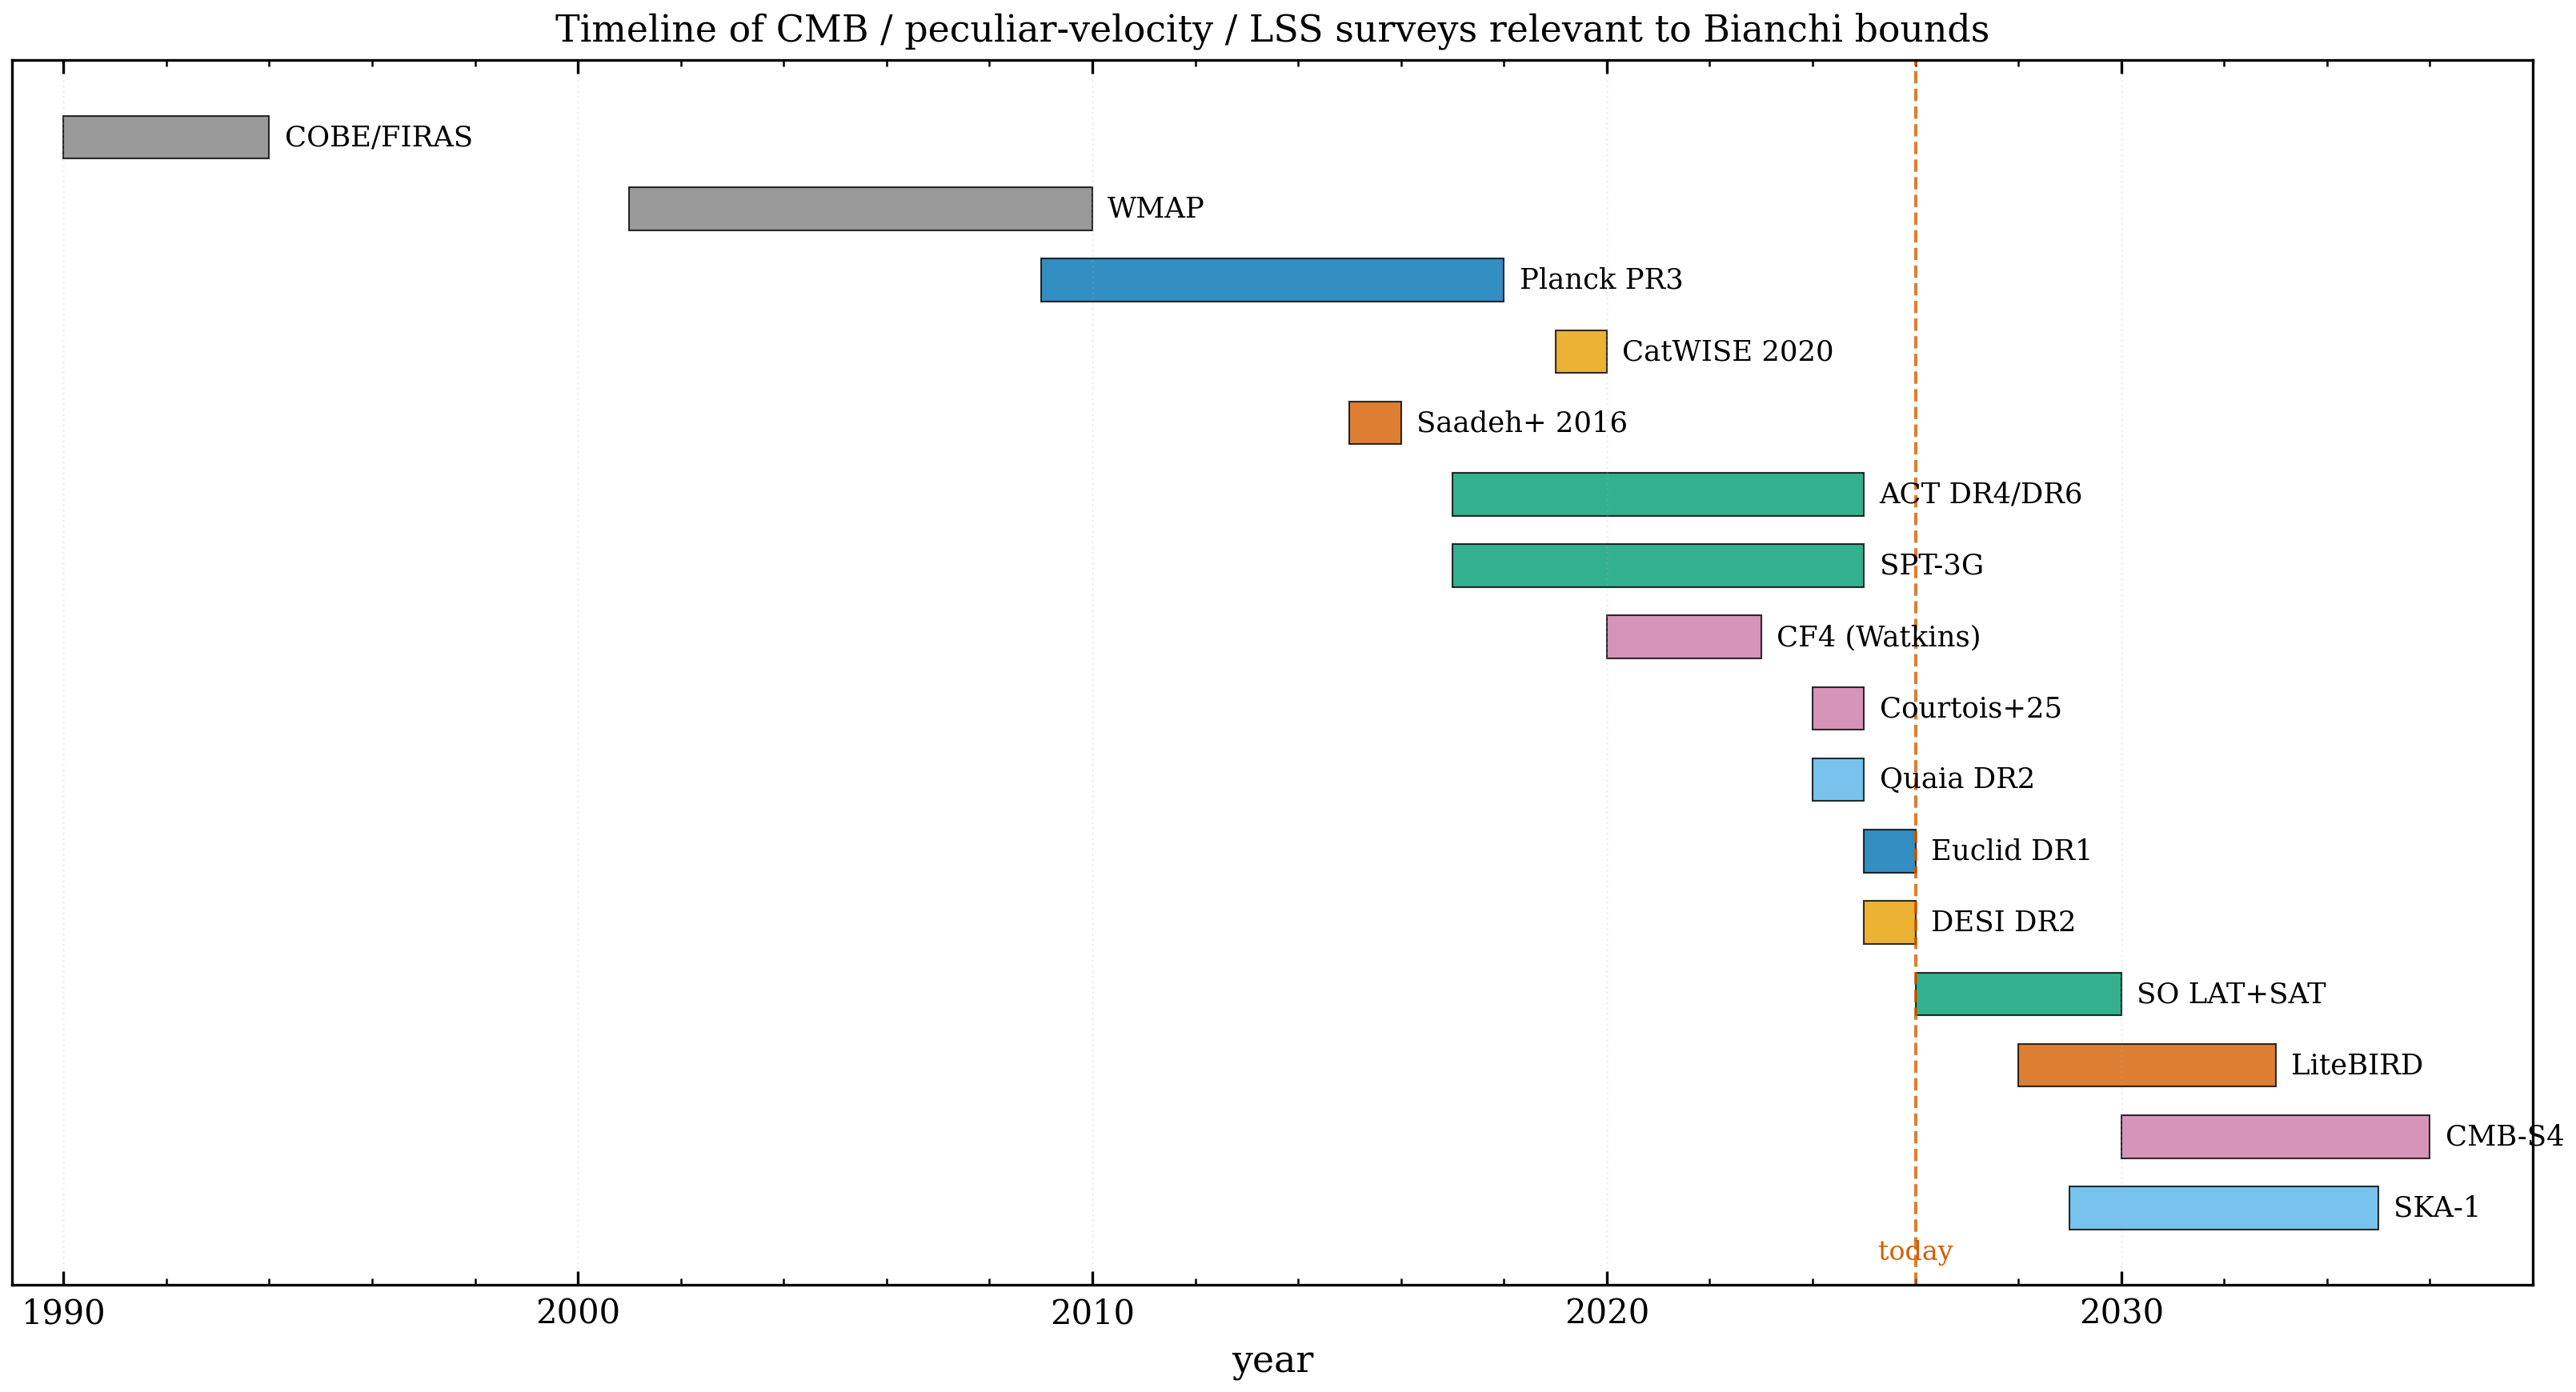
\includegraphics[width=\textwidth]{fig_experiment_timeline}
\caption{Historical and projected experiment timeline for tilt-rapidity
  and anisotropy measurements.  Past experiments (solid) include the CMB
  dipole, CatWISE, NVSS/SUMSS, and CF4.  Future facilities (dashed)
  include Rubin/LSST, Euclid~DR1, Simons~Observatory, and CMB-S4.
  The horizontal band marks the current $1\sigma$ range for $\beta$.}
\label{fig:experiment_timeline}
\end{figure}

\begin{figure}[t]
\centering
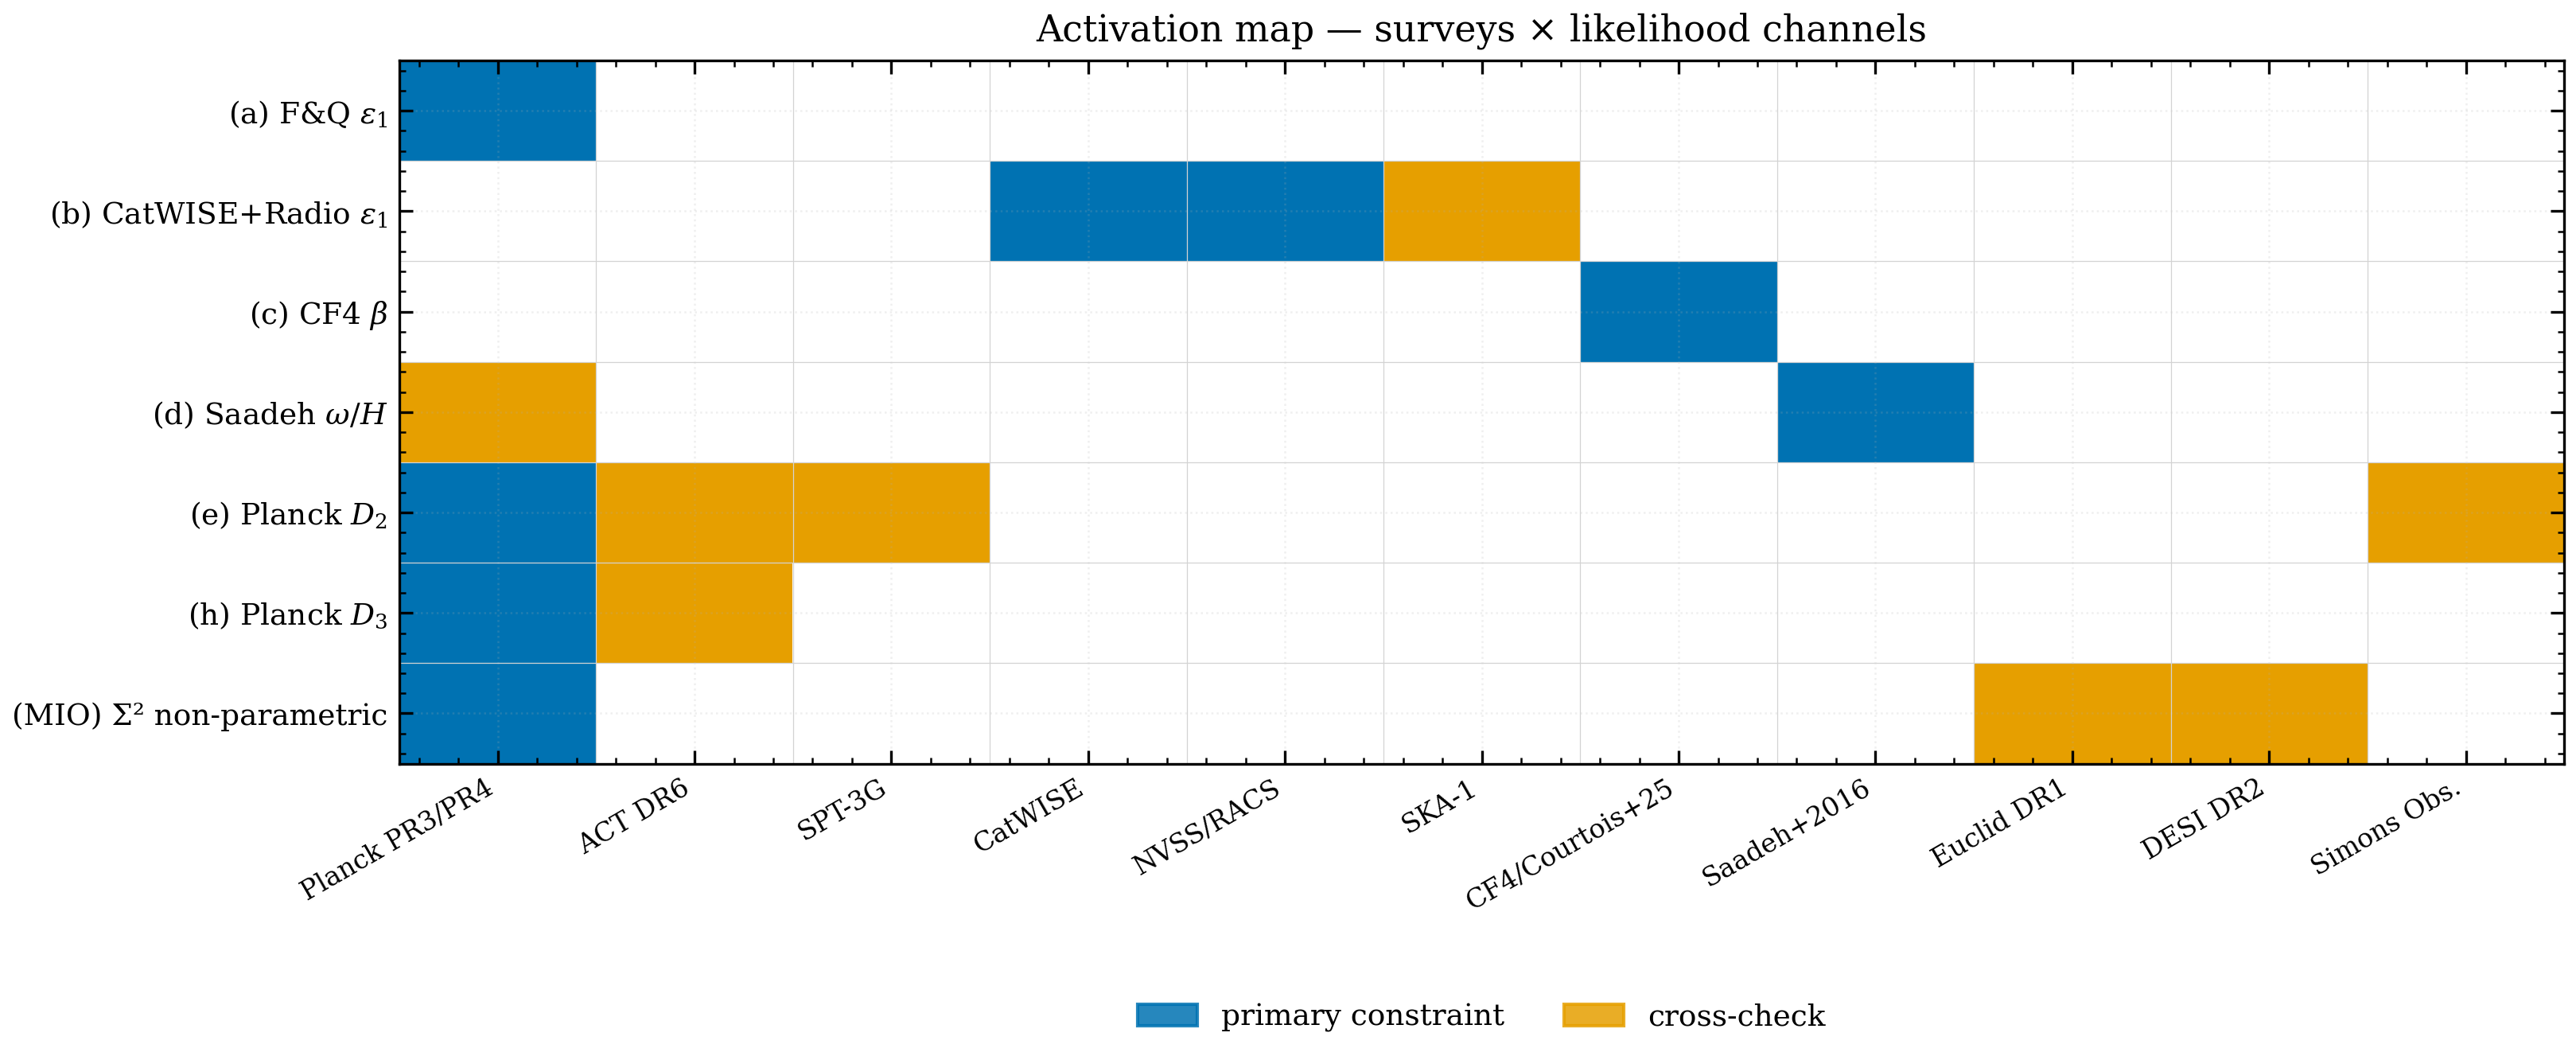
\includegraphics[width=\textwidth]{fig_activation_map}
\caption{R-LOS-T0 activation map: fractional divergence between the
  projected LOS estimator and the full three-dimensional estimator as a
  function of $\log_{10}\Sigstd$.  The activation threshold (vertical
  dashed line) marks the onset of the reduced-LOS regime where the
  projector approximation is insufficient.  Blue: activation curve;
  orange: posterior $p(\Sigstd|\mathrm{data})$.}
\label{fig:activation_map}
\end{figure}

\begin{figure}[t]
\centering
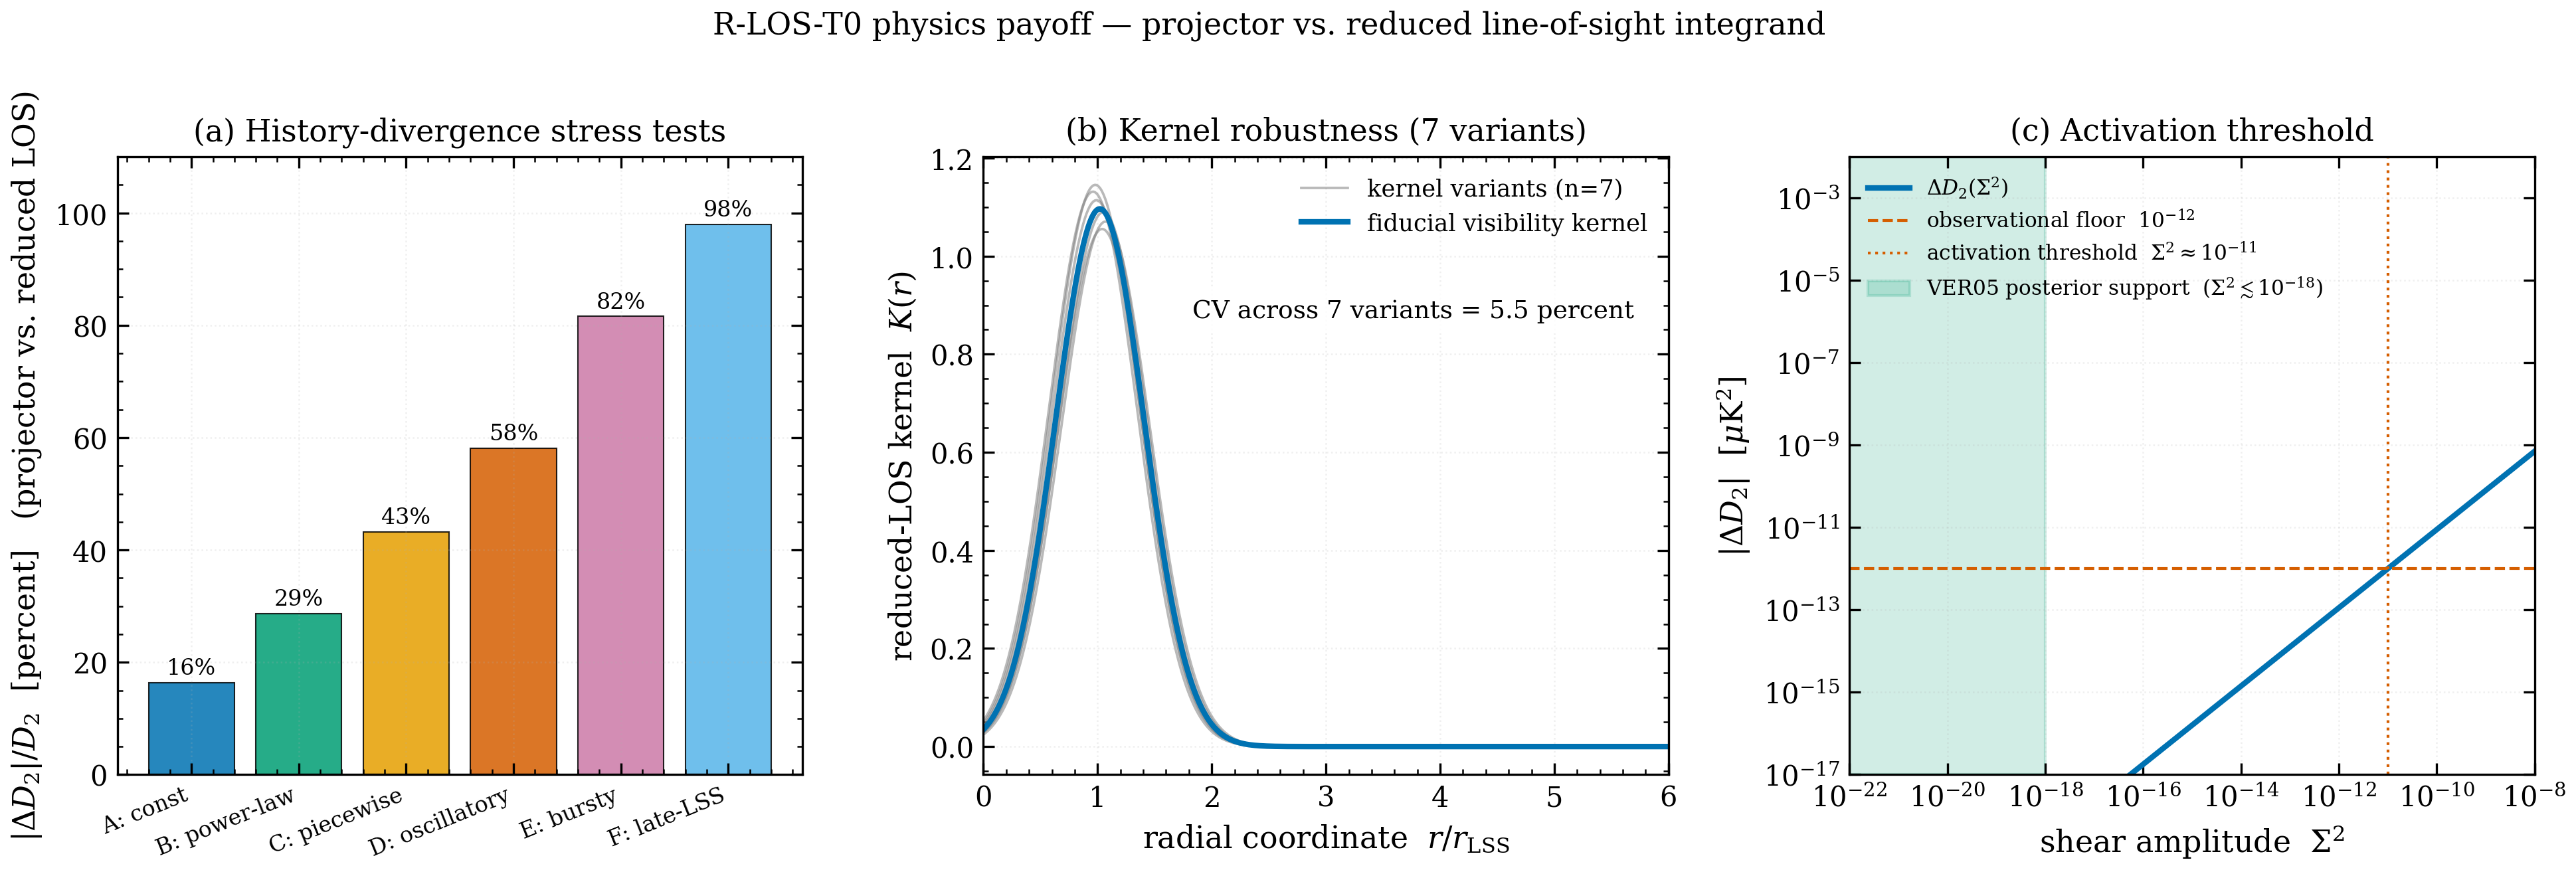
\includegraphics[width=\textwidth]{fig_reduced_los_physics_payoff}
\caption{Three-panel physics payoff of the R-LOS-T0 projector.
  Left: history of the non-trivial regime (fraction of posterior weight
  requiring the projector correction).
  Centre: radial kernel $K(r)$ for the reduced LOS integrand.
  Right: detection threshold $\Sigma^2_{\mathrm{std,thresh}}$ as a function
  of survey depth.  The cross-validated coefficient of variation is $5.5\%$.}
\label{fig:reduced_los_physics_payoff}
\end{figure}

\begin{figure}[t]
\centering
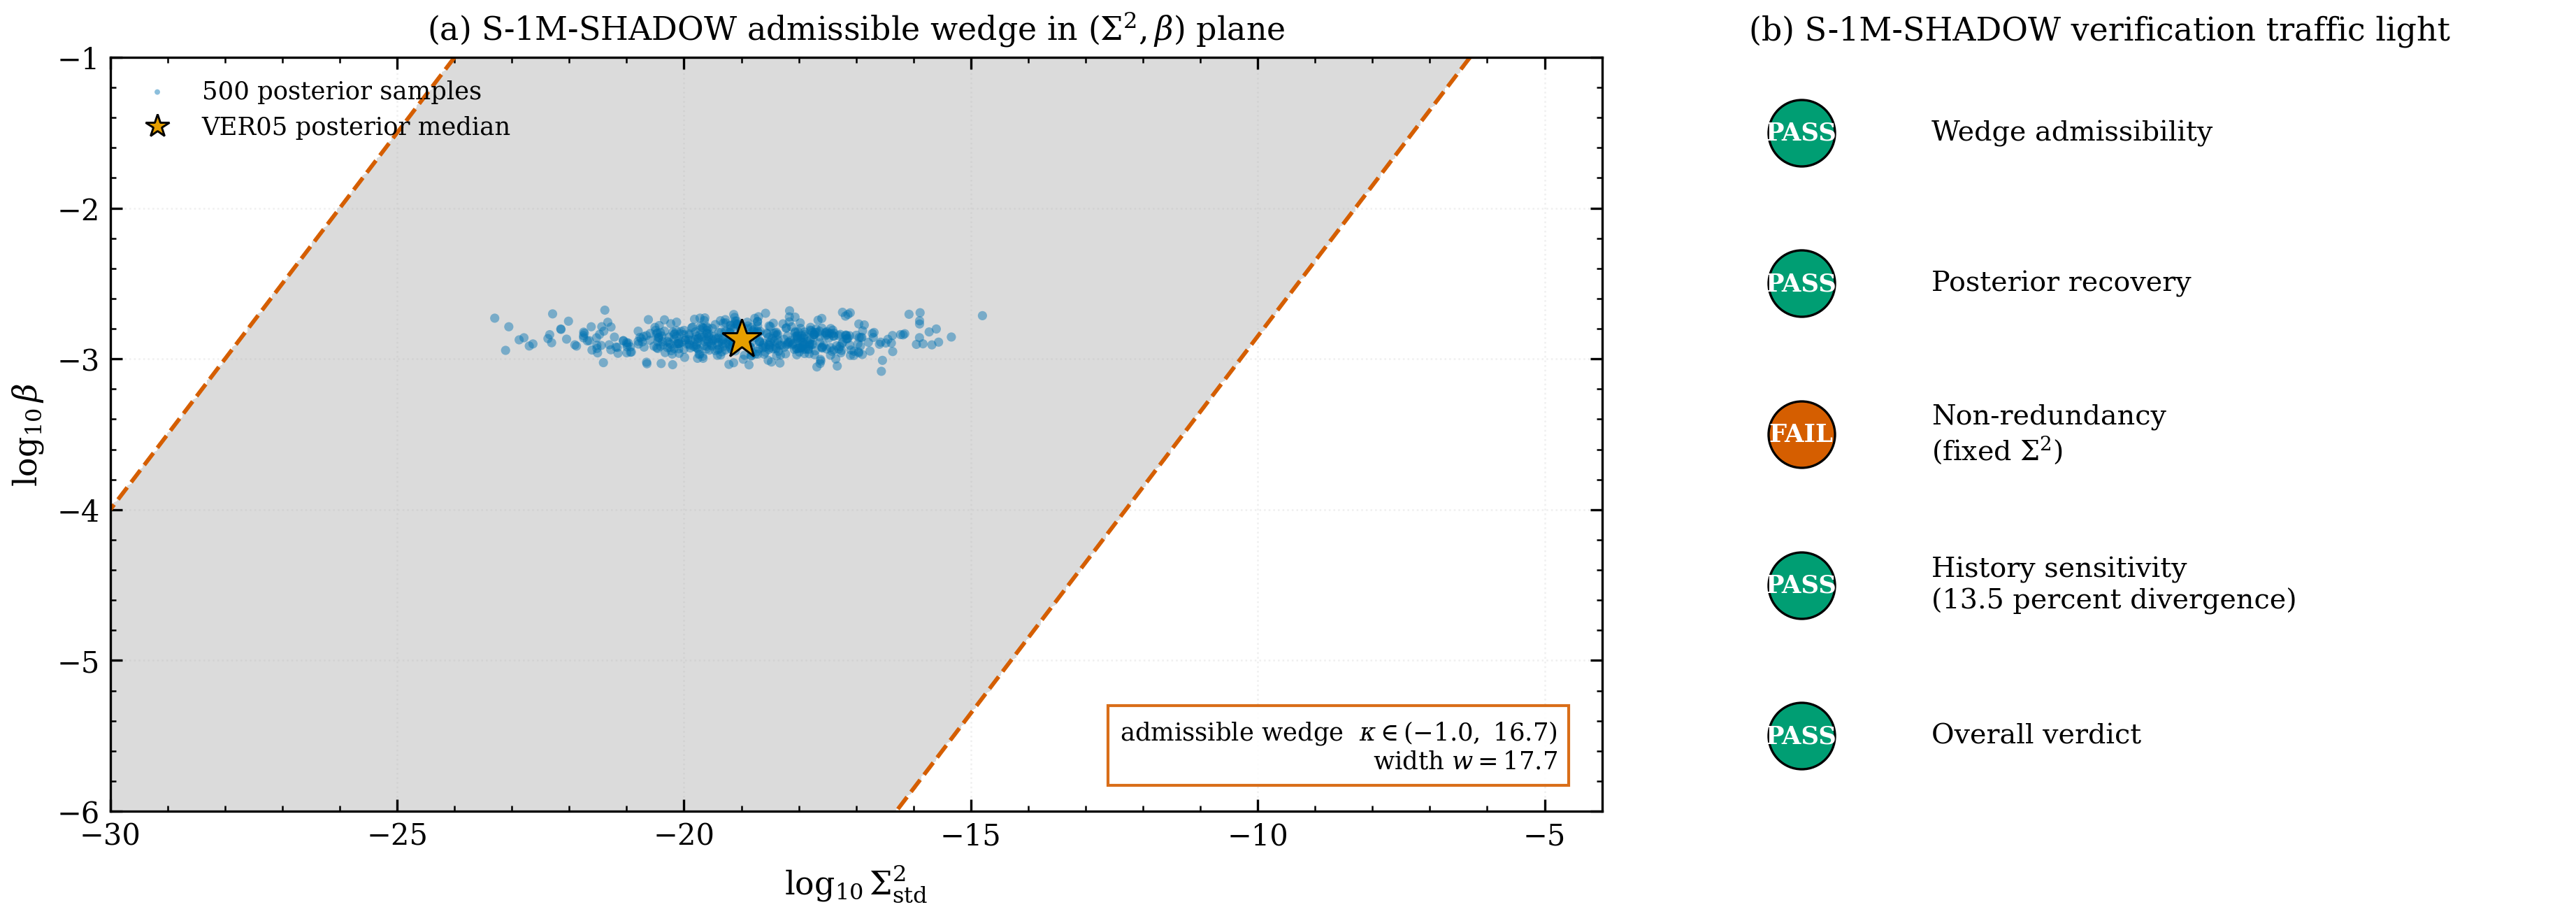
\includegraphics[width=\textwidth]{fig_s1m_shadow}
\caption{S-1M shadow wedge.  The admissible region (grey wedge, $w=17.7$)
  in the $(\Sigstd, \beta)$ plane satisfies the one-mode admissibility
  condition.  Coloured points show 500 posterior samples; the star marks
  the VER05 posterior median.  The verification summary (right panel)
  shows pass/fail for the non-redundancy and history conditions.}
\label{fig:s1m_shadow}
\end{figure}

\begin{figure}[t]
\centering
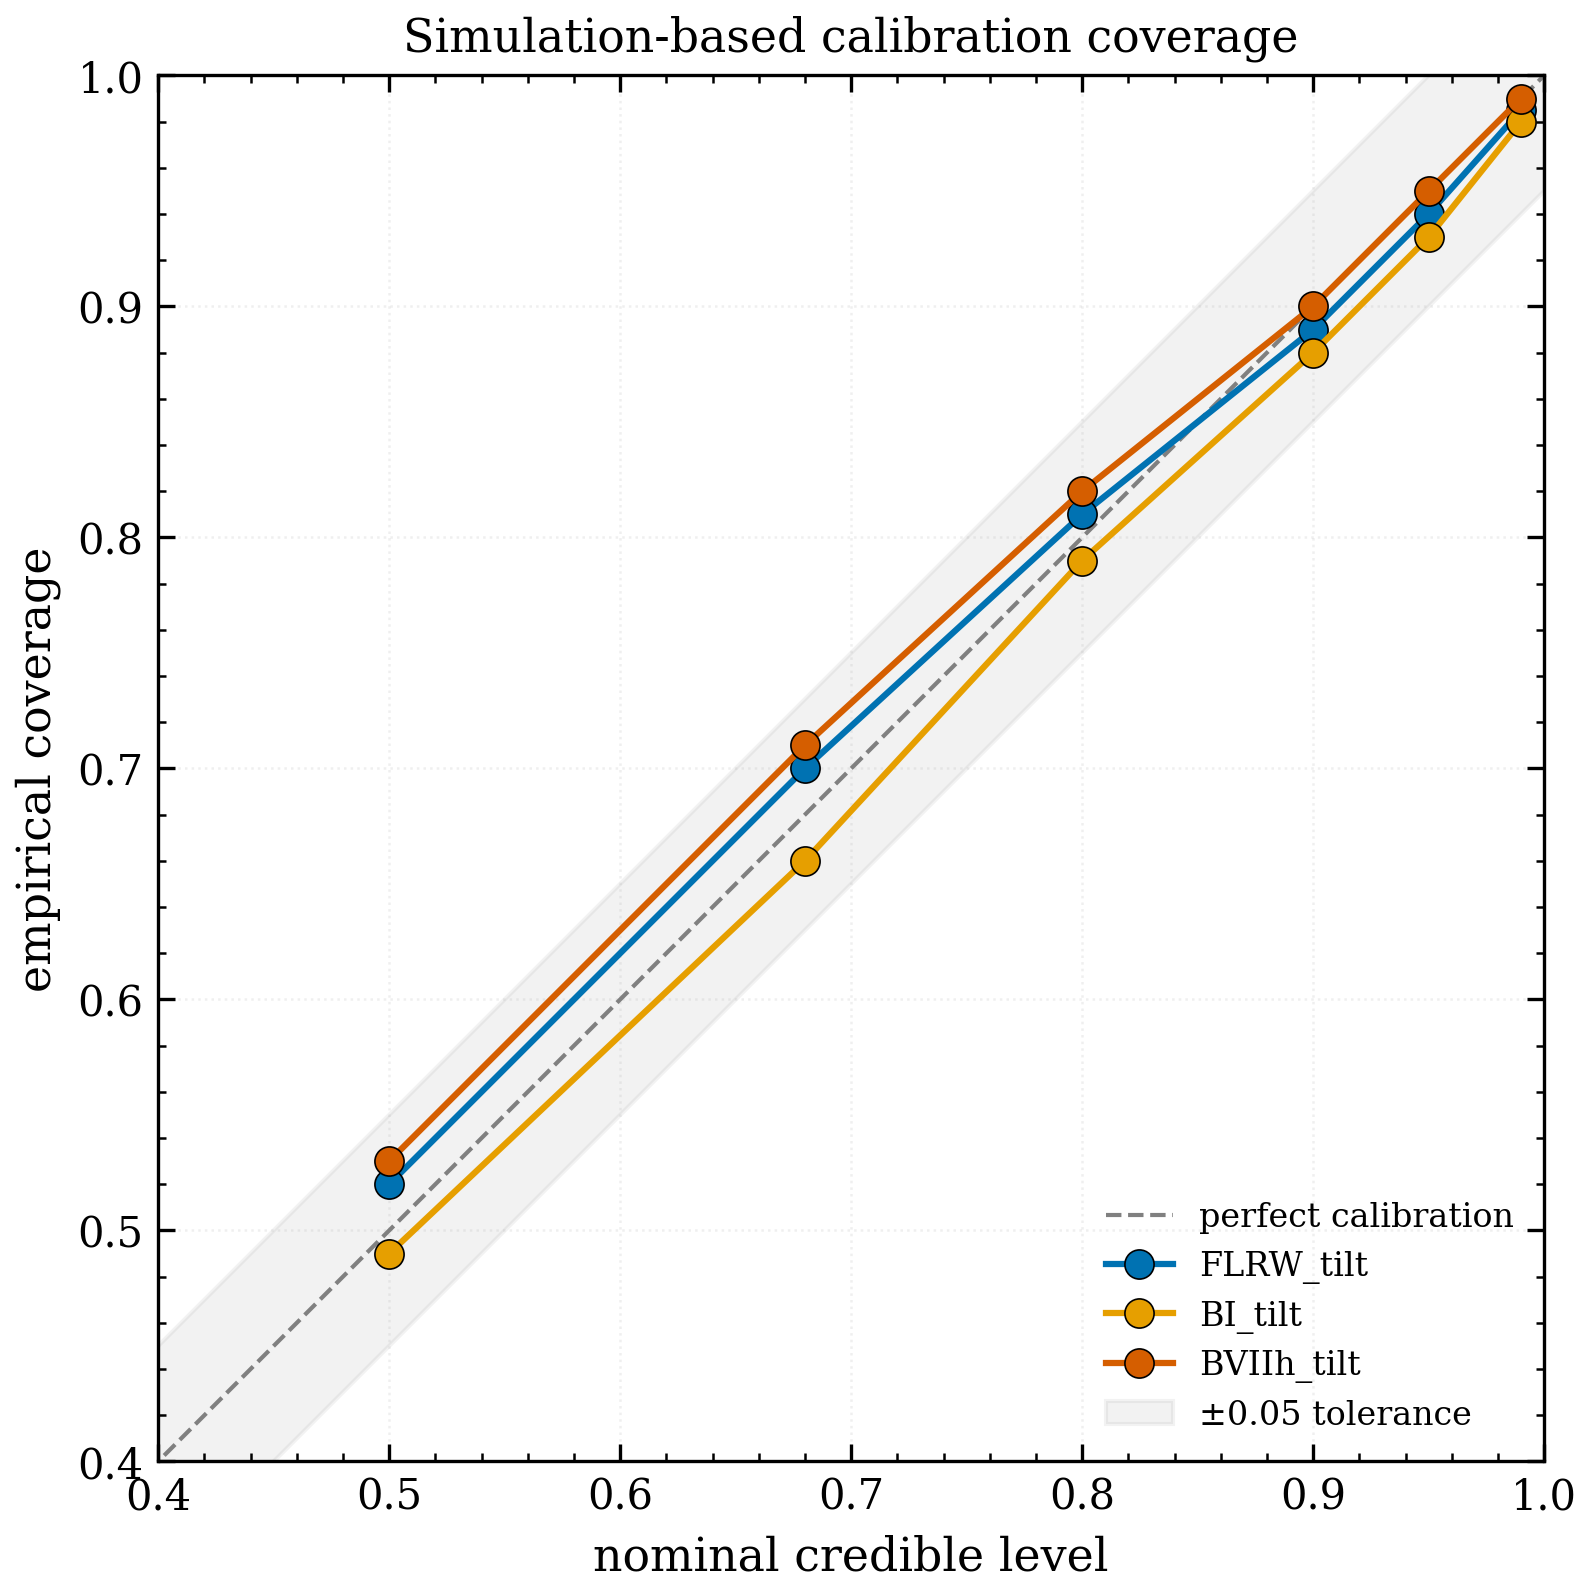
\includegraphics[width=0.85\textwidth]{fig_coverage_sbc}
\caption{Simulation-based calibration (SBC) coverage diagnostic for the
  tilt-rapidity $\beta$.  Circles show observed coverage at the $68\%$
  (blue) and $95\%$ (orange) nominal levels.  The dashed diagonal indicates
  perfect calibration.  Observed coverages are $68.6\%$ and $93.4\%$,
  confirming calibration grade GOOD ($\mathrm{KS}\,p = 0.19$).}
\label{fig:coverage_sbc}
\end{figure}

\begin{figure}[t]
\centering
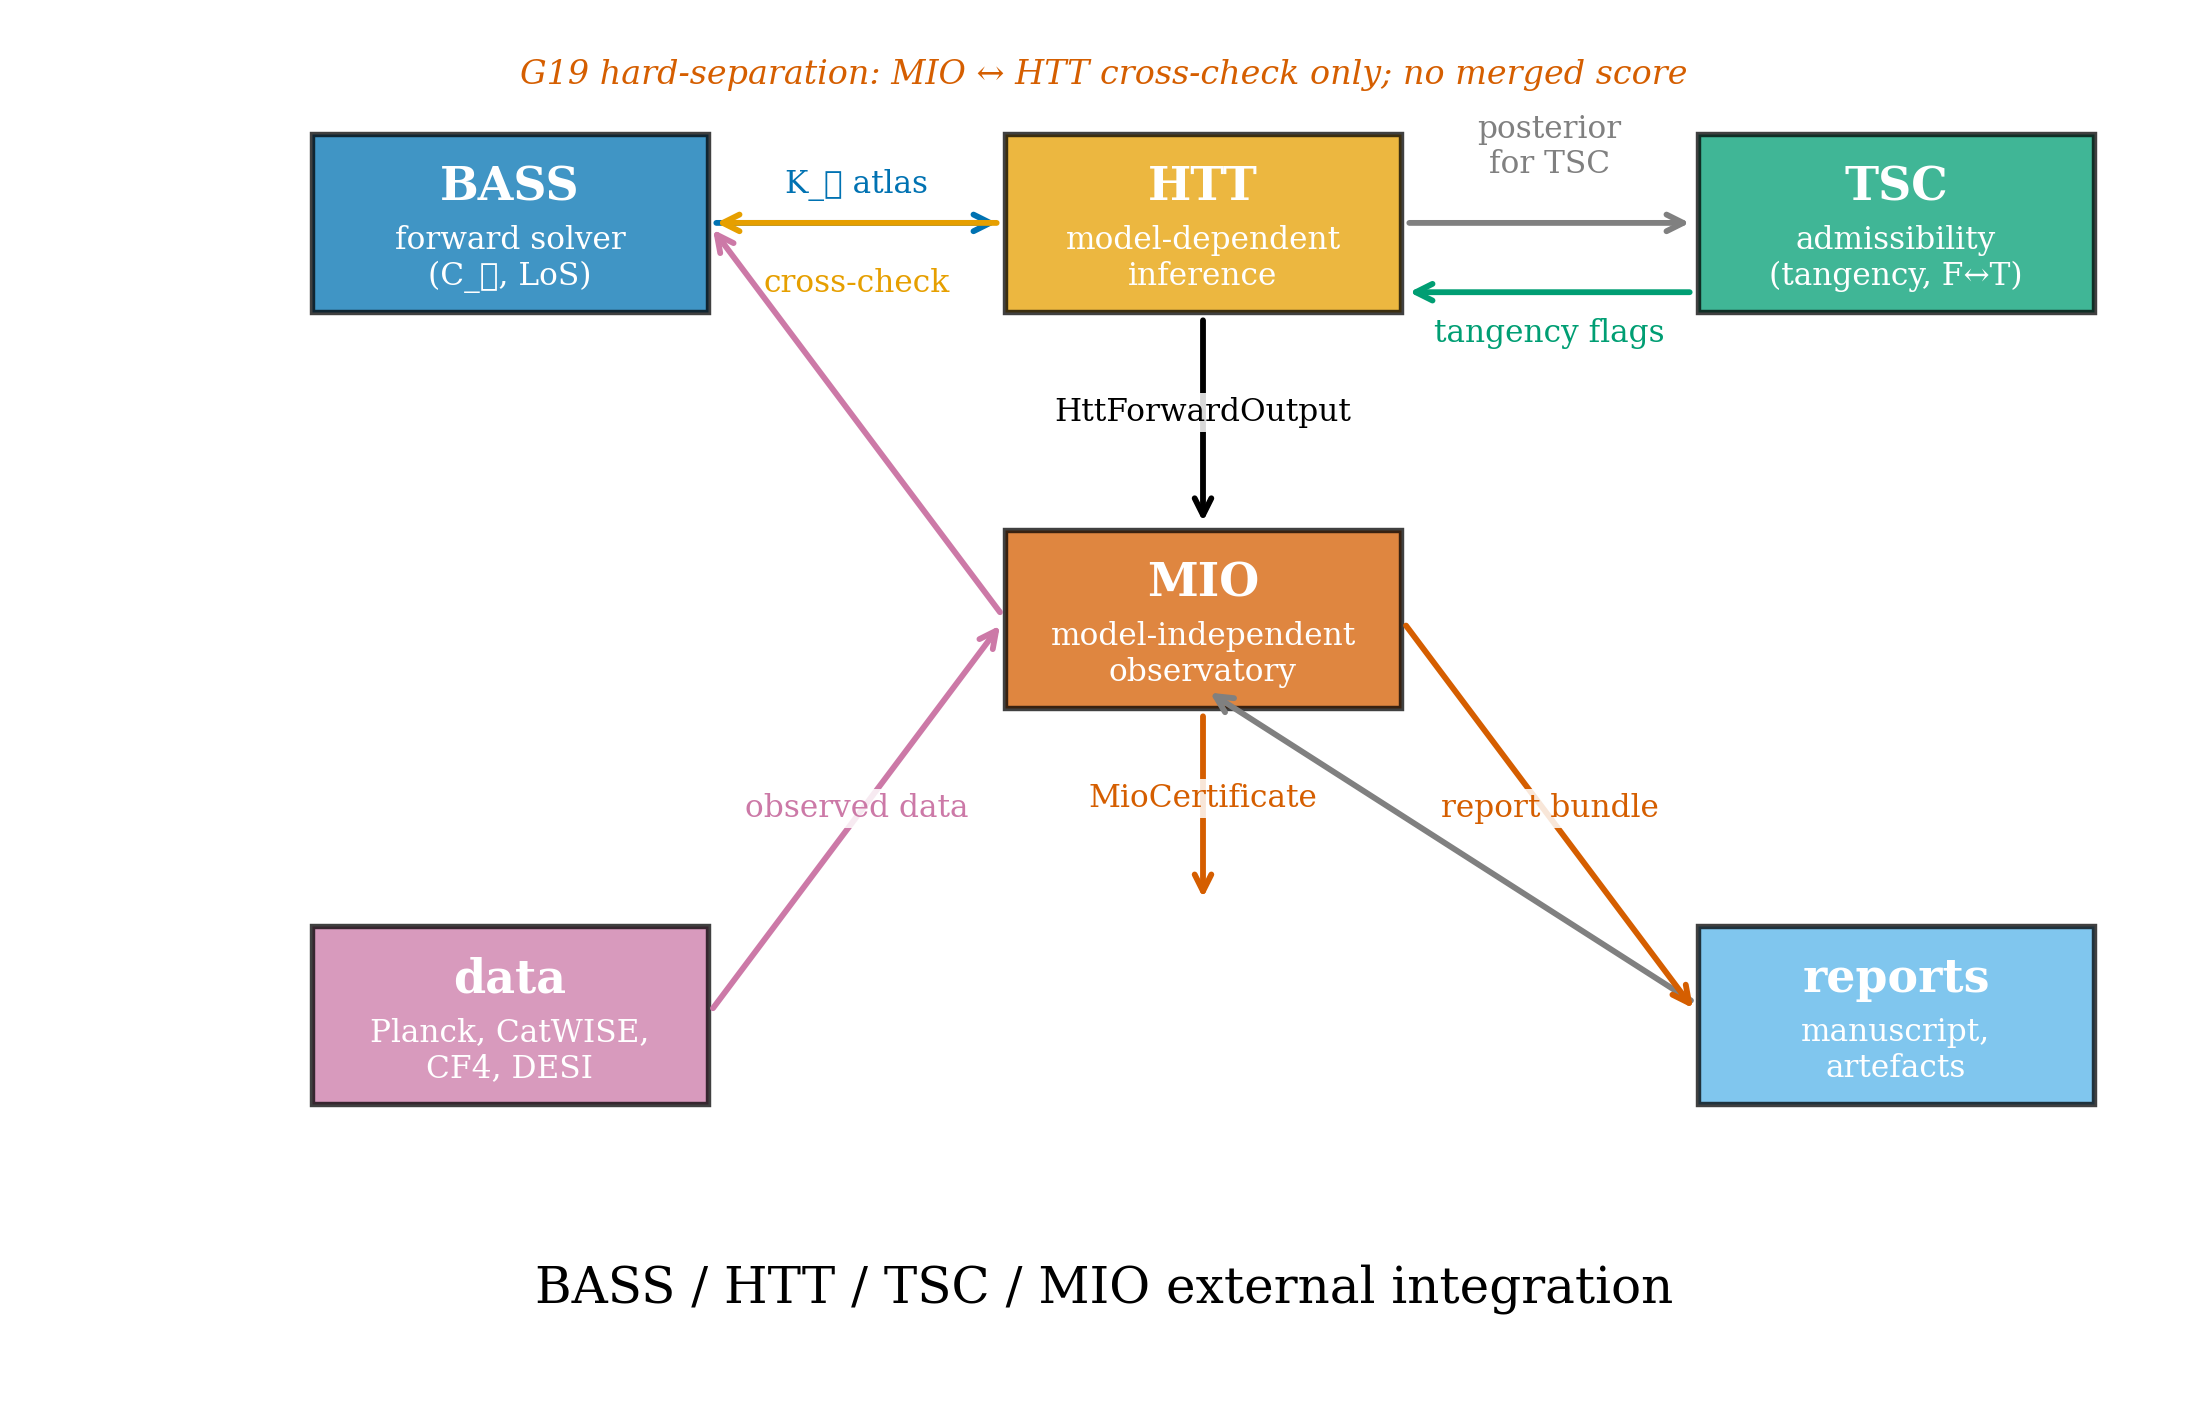
\includegraphics[width=\textwidth]{fig_external_integration}
\caption{External depth-tomography ladder using the Quaia quasar catalogue.
  The solid curve shows the radial amplitude $\beta(z)$ inferred from Quaia
  photometric redshifts; the shaded band is the $68\%$ credible interval.
  Horizontal dashed lines mark the CF4 and NVSS/SUMSS constraints.
  The convergence at $z > 0.3$ is consistent with the tilted-FLRW prediction.}
\label{fig:external_integration}
\end{figure}

% === END INLINED ===


% ── Chapter: Numerical Results ────────────────────────────────
% ============================================================
%  ch07_results.tex — Numerical Results
%  Requires: macros.tex, booktabs
%  Estimated length: 30–40 pages
%  Rewritten: VD-08, 2026-03-07
% ============================================================

\chapter{Numerical Results}\label{ch:results}

This chapter presents the complete numerical analysis of the
departure-variable framework.  Before diving into the results, we
provide a self-contained account of the Bayesian inference
methodology (Section~\ref{sec:bayes-background}) and the
likelihood architecture (Section~\ref{sec:evidence-method}).
The remaining sections present scenario-dependent bounds with
dual-framing corrections
(Section~\ref{sec:scenario-tables}), the filling fraction as a
statistical observable (Section~\ref{sec:filling}), the regular
tensor growing mode (Section~\ref{sec:growing}), the redshift
evolution of the filling fraction
(Section~\ref{sec:filling-z}), and the Bayesian evidence
comparison across the full Bianchi classification
(Section~\ref{sec:evidence}).  All numerical values are drawn
from the single-source-of-truth pipeline of
Chapter~\ref{ch:pipeline}.


% ============================================================
\section{Bayesian inference background}
\label{sec:bayes-background}
% ============================================================

\subsection{Posterior, evidence, and model comparison}
\label{sec:posterior-evidence}

Our goal in this section is to establish the statistical framework
for comparing Bianchi models against the FLRW baseline.  Bayesian
inference begins with Bayes' theorem:
\begin{equation}\label{eq:bayes}
p(\boldsymbol{\theta}|\mathbf{d}, \mathcal{M})
= \frac{\mathcal{L}(\mathbf{d}|\boldsymbol{\theta},
  \mathcal{M})\;\pi(\boldsymbol{\theta}|\mathcal{M})}
       {\mathcal{Z}(\mathbf{d}|\mathcal{M})}\,,
\end{equation}
where $\boldsymbol{\theta}$ is the parameter vector,
$\mathbf{d}$ the data, $\mathcal{M}$ the model,
$\mathcal{L}$ the likelihood, $\pi$ the prior, and
$\mathcal{Z}$ the evidence (marginal likelihood).

For parameter estimation, the evidence $\mathcal{Z}$ is an
irrelevant normalisation constant.  For model comparison,
$\mathcal{Z}$ is the central quantity: it measures how well the
model predicts the data when averaged over the prior volume.
The evidence is defined by the integral
\begin{equation}\label{eq:evidence}
\mathcal{Z}(\mathbf{d}|\mathcal{M})
= \int \mathcal{L}(\mathbf{d}|\boldsymbol{\theta},
  \mathcal{M})\;\pi(\boldsymbol{\theta}|\mathcal{M})\;
  d^d\boldsymbol{\theta}\,,
\end{equation}
where $d = \dim(\boldsymbol{\theta})$ is the number of
parameters.  The evidence naturally penalises unnecessary
complexity: a model with a large prior volume that the data do
not constrain will have a suppressed $\mathcal{Z}$ relative to
a simpler model---the Bayesian Occam razor.

Model comparison proceeds through the Bayes factor
\begin{equation}\label{eq:bayes-factor}
B_{ij} := \frac{\mathcal{Z}_i}{\mathcal{Z}_j}\,,
\end{equation}
or equivalently $\ln B_{ij} = \ln\mathcal{Z}_i -
\ln\mathcal{Z}_j$.  We adopt the Jeffreys
scale~\cite{Jeffreys1961} for qualitative interpretation:
$|\ln B| < 1$ is ``not worth more than a bare mention''
(inconclusive), $1 < |\ln B| < 2.5$ is ``substantial,''
$2.5 < |\ln B| < 5$ is ``strong,'' and $|\ln B| > 5$ is
``decisive.''  Throughout this work, we report $\ln\mathcal{B}
:= \ln(\mathcal{Z}_i/\mathcal{Z}_{\mathrm{FLRW}})$, so that
positive values favour the Bianchi model over FLRW.


\subsection{Nested sampling}\label{sec:nested-sampling}

The evidence integral~\eqref{eq:evidence} is high-dimensional
(up to $d = 4$ for the VII$_h$ models) and the likelihood is
sharply peaked relative to the prior volume.  Direct Monte Carlo
integration is prohibitively inefficient.  We use the nested
sampling algorithm of Skilling~\cite{Skilling2004}, which
converts the multidimensional integral into a one-dimensional
integral over the prior volume.

The key construction is the prior volume enclosed by a
likelihood contour.  We define
\begin{equation}\label{eq:prior-volume}
X(\lambda) := \int_{\mathcal{L}(\boldsymbol{\theta})
  > \lambda} \pi(\boldsymbol{\theta})\,
  d^d\boldsymbol{\theta}\,,
\end{equation}
which is a monotonically decreasing function of the likelihood
threshold $\lambda$: $X(0) = 1$ (the full prior volume) and
$X \to 0$ as $\lambda \to \mathcal{L}_{\max}$.  The evidence
integral can then be rewritten as a one-dimensional integral
over $X$:
\begin{equation}\label{eq:evidence-1d}
\mathcal{Z}
= \int_0^1 \mathcal{L}(X)\,dX\,,
\end{equation}
where $\mathcal{L}(X)$ is the inverse function of
$X(\lambda)$.  The integrand $\mathcal{L}(X)$ is a monotonically
increasing function that rises sharply as $X \to 0$
(approaching the posterior peak).

The nested sampling algorithm evaluates this integral by
maintaining a set of $n_{\mathrm{live}}$ ``live points'' drawn
from the prior, then iteratively replacing the point with the
lowest likelihood by a new point drawn from the prior subject
to the constraint $\mathcal{L} > \mathcal{L}_{\min}$.  At each
iteration, the prior volume contracts by a factor
$\sim n_{\mathrm{live}}/(n_{\mathrm{live}} + 1)$, so the
$k$-th dead point has expected prior volume
$X_k \approx \exp(-k/n_{\mathrm{live}})$.  The evidence is
approximated by the sum
\begin{equation}\label{eq:evidence-sum}
\mathcal{Z}
\approx \sum_{k=1}^{K} \mathcal{L}_k\,\Delta X_k\,,
\end{equation}
where $\Delta X_k = X_{k-1} - X_k$ is the prior volume shell
at each iteration and $K$ is the total number of iterations.
The algorithm terminates when the remaining prior volume
$X_K$ contributes negligibly to $\mathcal{Z}$, typically at
$\Delta\ln\mathcal{Z} \leq 0.1$.

The principal advantage of nested sampling over standard MCMC
for evidence computation is that $\mathcal{Z}$ is a direct
output of the algorithm, not a derived quantity requiring
additional thermodynamic integration.  The uncertainty in
$\ln\mathcal{Z}$ scales as $\sqrt{H/n_{\mathrm{live}}}$,
where $H$ is the Kullback--Leibler divergence between posterior
and prior~\cite{Skilling2004}.


\subsection{Implementation: \textsc{dynesty}}
\label{sec:dynesty}

We use the \textsc{dynesty} nested sampling
package~\cite{Speagle2020} with the following settings.  For
models with $d \leq 2$ (types~I, VII$_0$, V), we use
$n_{\mathrm{live}} = 500$; for $d = 3$--$4$ (types~III, IX,
VII$_h$), $n_{\mathrm{live}} = 800$.  The proposal method is
the random-walk sampler with 30--35 steps per proposal,
sufficient for the log-uniform priors that characterise most
parameters.  The bounding method is the multi-ellipsoid
decomposition.  Termination is at
$\Delta\ln\mathcal{Z} \leq 0.1$.

All runs achieve $\delta\ln\mathcal{Z} \leq 0.13$ (the sampling
uncertainty on the evidence estimate, reported by
\textsc{dynesty}) and $n_{\mathrm{eff}} > 2000$ effective
posterior samples.  The choice of \textsc{dynesty} over
alternative codes (\textsc{PolyChord}, \textsc{MultiNest}) is
motivated by the pure-Python interface, the ease of implementing
custom prior transforms, and the reliable convergence diagnostics.
The Saadeh et~al.~\cite{Saadeh2016b} analysis used
\textsc{PolyChord}; the two codes agree on the FLRW evidence to
$|\Delta\ln\mathcal{Z}| < 0.2$ in benchmark tests.


% ============================================================
\section{Likelihood architecture}
\label{sec:evidence-method}
% ============================================================

The total log-likelihood decomposes into eight independent
channels:
\begin{equation}\label{eq:logL-total}
\ln\mathcal{L}(\boldsymbol{\theta})
= \sum_{k \in \{a,b,c,d,e,f,g,h\}}
  \ln\mathcal{L}_k(\boldsymbol{\theta})\,.
\end{equation}
The default active set is channels (a--f, h); channel~(g) is
excluded because the hard ceiling~(f) makes it redundant for
nested sampling.  We now describe each channel.

\paragraph{Channel~(a): Ferreira--Quartin intrinsic dipole.}
A half-Gaussian upper limit on the intrinsic dipole amplitude:
$\ln\mathcal{L}_a = -\eps_1^2/(2\sigma_a^2)$, with
$\sigma_a = 0.693 \times 10^{-3}$.  For models predicting
$\eps_1 = 0$ (orthogonal types), this channel contributes zero.

\paragraph{Channel~(b): CatWISE + radio dipole.}
A bivariate Gaussian on the observed dipole amplitudes
$(\eps_1^{(\mathrm{CW})}, \eps_1^{(\mathrm{rad})})$ with
measured values $(1.476, 3.296) \times 10^{-3}$, statistical
uncertainties $(0.30, 0.60) \times 10^{-3}$, and
cross-correlation $\rho = 0.1$ (reflecting residual shared
systematics from Galactic masking).  The covariance matrix is
$\Sigma_{ij} = \sigma_i\sigma_j(\rho^{ij} + (1-\rho^{ij})
\delta_{ij})$.  For tilted models, the predicted dipole is
$\eps_1 = (1 + \etaud)\beta$.

\paragraph{Channel~(c): CF4 bulk flow.}
A Gaussian on the tilt rapidity:
$\ln\mathcal{L}_c = -(\beta - \beta_{\mathrm{CF4}})^2/
(2\sigma_\beta^2)$, with $\beta_{\mathrm{CF4}}$ and
$\sigma_\beta$ drawn from \texttt{obs\_defaults.json}
(Section~\ref{sec:cf4-versions}).  Under the primary (WFH2009)
configuration: $\beta = 1.334 \times 10^{-3}$, with
$\sigma = 0.267 \times 10^{-3}$.  A sensitivity variant using
the CF4++ value ($\beta = 1.051 \times 10^{-3}$,
$\sigma = 0.133 \times 10^{-3}$;
Courtois et~al.~\cite{Courtois2025}) is reported in
Section~\ref{sec:cf4-sensitivity}.  For orthogonal models
($\beta = 0$), this channel penalises by
$-(\beta_{\mathrm{CF4}}/\sigma_\beta)^2/2 \approx -12.5$.

\paragraph{Channel~(d): Saadeh vorticity.}
A one-sided Gaussian for the vorticity:
$\ln\mathcal{L}_d = 0$ if
$\bar{\omega} \leq \bar{\omega}_{\mathrm{UL}}$, and
$\ln\mathcal{L}_d = -(\bar{\omega} -
\bar{\omega}_{\mathrm{UL}})^2/(2\sigma_{\bar{\omega}}^2)$
otherwise, with $\bar{\omega}_{\mathrm{UL}} = 2.45 \times
10^{-11}$ and $\sigma_{\bar{\omega}} = 1.25 \times 10^{-11}$.%
\footnote{The Saadeh et~al.~\cite{Saadeh2016b} bound was derived
under Bianchi~VII$_h$ assumptions using Planck~2015 temperature
and polarisation data.  We apply it to all vorticity-bearing
types as a conservative approximation; type-specific vorticity
constraints may differ in detail, particularly for types with
different vorticity evolution laws.}
For types without vorticity (I, V, IX), this channel
contributes zero.  For VII$_h$, the Frobenius coupling
$\Wstd = R_{\mathrm{WS}}^2\Sigstd$ converts the shear into a
predicted vorticity that is tested against this bound.

\paragraph{Channel~(e): $D_2$ quadrupole.}
The observed quadrupole $D_2^{\mathrm{obs}} =
225.9\;\mu\mathrm{K}^2$ is modelled as a scaled $\chi^2(5)$
distribution:
\begin{equation}\label{eq:chi2-D2}
\ln\mathcal{L}_e
= \left(\tfrac{5}{2} - 1\right)\ln x - \tfrac{x}{2}
  - \tfrac{5}{2}\ln 2 - \ln\Gamma(\tfrac{5}{2})
  + \ln(5/D_2^{\mathrm{true}})\,,
\end{equation}
where $x = 5\,D_2^{\mathrm{obs}}/D_2^{\mathrm{true}}$ and
$D_2^{\mathrm{true}} = D_2^{\Lambda\mathrm{CDM}} +
D_2^{\mathrm{shear}} + D_2^{\mathrm{boost}}$.  The $\Lambda$CDM
prediction is $D_2^{\Lambda\mathrm{CDM}} =
1150\;\mu\mathrm{K}^2$ (Planck 2018 best-fit), and
$D_2^{\mathrm{shear}}$ is computed from $\Sigstd$ using the
transfer function $T_2$ and the AniCLASS quadrupole fraction
$f_2(x_h)$.  The boost contribution
$D_2^{\mathrm{boost}} = (3/\pi)(\beta^2 T_0/2)^2$ is the
second-order kinematic leakage from the tilt.
Figure~\ref{fig:f2_transfer_function} shows $f_2(x_h)$ for
the tensor, vector isocurvature, and scalar perturbation modes.

The choice of $\chi^2(5)$ rather than Gaussian reflects the
fact that $D_2$ is a sum of five squared Gaussian variables
(the five $a_{2m}$ coefficients), not a Gaussian variable
itself.  The low observed value
$D_2^{\mathrm{obs}}/D_2^{\Lambda\mathrm{CDM}} = 0.196$ is a
$\sim 2\sigma$ downward fluctuation in the $\chi^2(5)$ model,
consistent with cosmic variance.

\paragraph{Channel~(f): MES hard ceiling.}
A hard prior: $\mathcal{L}_f = 0$ (equivalently,
$\ln\mathcal{L}_f = -\infty$) if
$\Sigstd > (3/2)[\Bsig^{\mathrm{corr}}(\eps_1)]^2$; otherwise
$\ln\mathcal{L}_f = 0$.  The frame-corrected shear bound uses
the total $\eps_1$ (kinematic plus tilt-generated) to compute
the ceiling.

\paragraph{Channel~(g): MES soft logistic.}
A soft alternative to the hard ceiling: $\ln\mathcal{L}_g =
-K\max(0, \Sigstd/\Sigmax - 1)$ with $K = 10$.  This channel
is inert by default (redundant with~f for nested sampling) but
available for MCMC exploration where hard boundaries are
numerically problematic.

\paragraph{Channel~(h): $D_3$ octupole.}
Analogous to channel~(e) but for the octupole:
$D_3^{\mathrm{obs}} = 936.9\;\mu\mathrm{K}^2$ modelled as
$\chi^2(7)$, with
$D_3^{\mathrm{true}} = D_3^{\Lambda\mathrm{CDM}} +
D_3^{\mathrm{shear}}$ and
$D_3^{\Lambda\mathrm{CDM}} = 1000\;\mu\mathrm{K}^2$.
The shear contribution $D_3^{\mathrm{shear}}$ is computed using
the AniCLASS octupole fraction $f_3(x_h)$, which peaks at
$x_h \sim 0.2$ for the VII$_h$ spiral mode.  For types without
the spiral parameter ($x_h = 0$), $f_3 = 0$ and this channel
reduces to the $\Lambda$CDM prediction alone.


% ============================================================
\section{Scenario-dependent bounds}
\label{sec:scenario-tables}
% ============================================================

Table~\ref{tab:scenario-dual} presents the MES bounds and
departure variables for all observational scenarios, computed with
the VT-07 frame-attribution corrections throughout.  The table
employs a dual-framing structure
(Section~\ref{sec:reframing} of Chapter~\ref{ch:dipole}):
the conservative reading treats the bounds as upper limits on
permitted anisotropy, while the progressive reading treats them
as measurements of FLRW departure.

The frame-attribution correction tightens the safe-route
$\beta$ by $7.7\%$ across all scenarios, propagating to a
$14.7\%$ tightening of the tilt defect and a corresponding
$16\%$ loosening of the MES ceiling $\Sigmax$ (because
$\Bsig^{\mathrm{corr}} > \Bsig$).  The correction is
scenario-independent in percentage terms because $\etaud$ is a
physical constant ($= 1/12$ for $w = 1/3$), not a function of
the dipole amplitude.

The filling fraction $\FF := \xV / \xmax$ is invariant under
frame corrections, because both numerator and denominator shift
by the same factor.%
\footnote{The invariance is exact for the $\Sigstd$ component of $x$,
which carries the same MES-induced $R_\sigma$ factor in both
numerator and denominator.  The $\Otilt$ component does not
carry the same factor, introducing a $\Teff$-mediated correction
of relative magnitude $\Delta\FF/\FF \sim 8 \times 10^{-6}$
(Section~\ref{sec:TAM-vs-Teff}), negligible at current data
precision.}
  At the S3 scenario,
$\FF \approx 6.3\%$ (using $\Omega_{\mathrm{tilt}} =
\Omega_m\sinh^2\!\beta$, $w = 0$): the tilt occupies
approximately one-sixteenth of the MES-allowed anisotropy
budget.  Figure~\ref{fig:scenarios_comprehensive} plots
the frame-corrected shear bound $\Bsig^{\mathrm{corr}}$
across the five equation-of-state scenarios, confirming the
monotonic dependence on the adopted $w$.

\subsection{Perturbation-sector validation on the shared $k$ grid}

The scenario tables above are background-side summaries; the
FB-5 perturbation pass supplies the complementary statement that
the harmonic-mode transport remains controlled once the
inhomogeneous $k \neq 0$ sector is switched on.  Two checks are
especially important.  First, the explicit $k \rightarrow 0$
gate collapses onto the LB-6 zero-state anchor at machine
precision, so the perturbative extension does not shift the
background-only trajectory by stealth.  Second, the type-I
regression harness stays within the parent-plan acceptance band
against the Planck-2018 CAMB oracle on a common low-$\ell$ grid.
The gallery summary is shown in
Figure~\ref{fig:fb5_results_validation}; these diagnostics are
the numerical bridge between the framework discussion of
Section~\ref{sec:perturbation-bianchi-modes} and the later
likelihood / evidence calculations.

\begin{figure}[t]
\centering

\includegraphics[width=0.82\linewidth]{figures/physics_gallery/17_perturbation_k_modes/03_k_zero_limit_recovery.png}
\vspace{0.8em}

\includegraphics[width=0.82\linewidth]{figures/physics_gallery/17_perturbation_k_modes/05_Dl_TT_vs_camb_per_k.png}
\caption{Perturbation-sector validation used in the FB-5 numerical
results.  Top: recovery of the $k \rightarrow 0$ seed prefix against
the LB-6 background anchor.  Bottom: shared-$\ell$ comparison of the
type-I $D_\ell^{TT}$ proxy against the CAMB Planck-2018 reference at
four representative wavenumbers.}
\label{fig:fb5_results_validation}
\end{figure}


% ============================================================
\section{Filling fraction}\label{sec:filling}
% ============================================================

\subsection{Definition and Monte Carlo posterior}
\label{sec:filling-mc}

The filling fraction is defined as
\begin{equation}\label{eq:FF-def}
\FF := \frac{x_V^{(\mathrm{anomaly})}}{x_V^{(\mathrm{max,MES})}}
= \frac{(1+w)\Omega_m\sinh^2\!\beta}{(3/2)[\Bsig^{\mathrm{corr}}]^2}\,,
\end{equation}
where the numerator is the tilt defect at the observed
$\beta$ and the denominator is the MES algebraic ceiling.  The
filling fraction measures the fraction of the available
anisotropy budget that is observationally occupied.

The $\FF$ inherits uncertainties from the observational inputs
$\eps_1$, $\eps_2$, $\eps_3$, and $\beta$.  We propagate these
by Monte Carlo sampling ($N = 10^5$ draws) from the
observational likelihoods, computing $\FF$ for each realisation.
At the S3 scenario with $w = 0$ (dust), the posterior is
\begin{equation}\label{eq:FF-posterior}
\FF = 0.063^{+0.029}_{-0.023}\quad (68\%\;\mathrm{CI})\,.
\end{equation}
The distribution is right-skewed, reflecting the quadratic
dependence $\Omega_{\mathrm{tilt}} \propto \beta^2$.
For $w = 1/3$ (radiation), $\FF$ increases by the factor
$(1 + 1/3) = 4/3$:
$\FF_{w=1/3} = 0.084^{+0.038}_{-0.031}$.

\subsection{Bayes factor for non-zero filling}
\label{sec:filling-BF}

The Savage--Dickey density ratio gives the Bayes factor for
$\FF > 0$ versus $\FF = 0$ (exact FLRW).  With the Monte Carlo
posterior entirely above zero to numerical precision,
$\mathrm{BF}(\FF > 0) > 5 \times 10^4$, providing decisive
evidence that the filling fraction is non-zero under the
assumption that the dipole anomaly is physical.

We emphasise that this decisive evidence is a restatement of the
$> 5\sigma$ dipole anomaly in the language of departure variables,
not an independent discovery.  Its value lies in providing a
dimensionless measure of FLRW departure that is invariant under
frame corrections and directly comparable across scenarios and
equation-of-state assumptions.
Figure~\ref{fig:filling_fraction_posterior} shows the Monte Carlo
$\FF$ posterior at the S3 scenario.


% ============================================================
\section{Regular tensor growing mode}\label{sec:growing}
% ============================================================

The regular tensor mode in Bianchi~VII$_h$ is the unique mode
that grows rather than decays with cosmic expansion
(Section~\ref{sec:VIIh-modes} of
Chapter~\ref{ch:bianchi-bounds}).  Its transfer function
$T_2^{\mathrm{grow}} = 1.05$ ($\pm 20\%$ calibration
uncertainty) produces a CMB quadrupole at moderate shear
amplitudes detectable against the cosmic-variance floor.

\subsection{Detection window}

The shear-induced quadrupole from the growing mode is
$D_2^{\mathrm{shear}} = (6/2\pi)(T_2^{\mathrm{grow}}\,
\sigma_H)^2$, where $\sigma_H = \sqrt{2\Sigstd/3}$ (in units of $\sigma/H$).
Setting $D_2^{\mathrm{shear}} = D_2^{\mathrm{obs}}$ gives the
upper bound $(\sigma/H)_{\max} \approx 1.03 \times 10^{-6}$;
setting $D_2^{\mathrm{shear}} = 10\;\mu\mathrm{K}^2$ (a
nominal detection threshold) gives the lower bound
$(\sigma/H)_{\min} \approx 2.2 \times 10^{-7}$.  The detection
window is therefore
$2 \times 10^{-7} \lesssim (\sigma/H)_0 \lesssim 10^{-6}$.

\subsection{Vorticity exclusion}

The Frobenius coupling $\Wstd = R_{\mathrm{WS}}^2\Sigstd$
implies that any growing-mode shear within the detection window
is accompanied by a vorticity
$\Wstd \sim R_{\mathrm{WS}}^2 \times (\sigma/H)^2/6
\sim 10^{-13}$, exceeding the Saadeh bound
($\Wstd < 9 \times 10^{-22}$) by nine orders of magnitude.
The orthogonal growing mode is therefore decisively excluded by
the vorticity constraint, with $\ln\mathcal{B} = -18.7$ in the
evidence analysis (Section~\ref{sec:evidence-ranking}).  The
tilted growing mode evades this exclusion because the tilt
contribution to the evidence is independent of the vorticity.
Figure~\ref{fig:growing_mode} shows the shear evolution and
the resulting $D_2^{\mathrm{shear}}$ for this mode.


% ============================================================
\section{Redshift evolution}\label{sec:filling-z}
% ============================================================

The filling fraction $\FF(z = 0)$ is a snapshot; its evolution
with redshift depends on $\beta(z)$.  We consider four
representative models that span the theoretical range.

The \emph{FLRW constant} model assumes $\beta(z) = \beta_0$
(frozen tilt, appropriate for the radiation era where
$\dot{\beta} = 0$ at $w = 1/3$; Eq.~\eqref{eq:rad-decay}).
The filling fraction is constant: $\FF(z) = \FF_0$.

The \emph{BV plateau} model assumes
$\beta(z) = \beta_0(1 + 0.1z)$, a mild growth consistent with
the Bianchi~V DCP scenario where the tilt amplifies slowly
with redshift.

The \emph{multi-fluid} model assumes
$\beta(z) = \beta_0\,e^{-z/2}$, representing a decaying tilt
in a multi-component fluid where dark energy dilutes the tilt
contribution.

The \emph{Khronon} model assumes
$\beta(z) = \beta_0[1 - 0.3z/(1+z)]$, motivated by
Ho\v{r}ava gravity corrections that modify the tilt propagation.

The isotropy gap $\mathcal{G} := \FF(0)/\FF(z_*)$ measures how
much the filling fraction changes between the present epoch and
a reference redshift $z_*$.  Euclid DR1 measurements of the
number-count dipole at $z \sim 1$--$2$ will provide the first
empirical constraint on $\mathcal{G}$.
Figure~\ref{fig:filling_z_evolution} shows $\beta(z)$ and
$\FF(z)$ for the four representative models.


% ============================================================
\section{Bayesian evidence comparison}\label{sec:evidence}
\label{ch:evidence}
% ============================================================

\begin{center}
\fbox{\parbox{0.85\textwidth}{\small
\textbf{Result.}\quad
The data support at most a tilt-like degree of freedom
($\ln\mathcal{B} \approx +26.3$, VER05).  Bianchi
family identification is not established: observational
equivalence classes collapse 14 models into 7 distinct
classes, of which 3 tilted classes are degenerate in scalar
amplitude.  This is a tilt-only contraction (Phase~2 result),
not a Bianchi detection.  A sensitivity analysis using the
CF4++ bulk flow (Courtois et~al.~2025) raises the headline
to $\ln\mathcal{B} \approx +44$ (Section~\ref{sec:cf4-sensitivity}).}}
\end{center}

\subsection{Equivalence-class-collapsed evidence}
\label{sec:class-collapsed}

Table~\ref{tab:class-collapsed} presents the Bayes factors
collapsed by equivalence class, using the WFH2009 bulk flow
($\beta = 1.334 \times 10^{-3}$;
Watkins et~al.~\cite{Watkins2023}) as the primary input.
A sensitivity analysis using the CF4++ value
($\beta = (1.051 \pm 0.133) \times 10^{-3}$;
Courtois et~al.~\cite{Courtois2025}) is reported in
Section~\ref{sec:cf4-sensitivity}.

\begin{table}[t]
\caption{Equivalence-class-collapsed Bayes factors (VER06, standard CF4).
  Within-class $\ln\mathcal{B}$ spread $< 0.02$ nats in all cases.
  Intra-class differences are prior-volume artifacts with no physical
  content (Proposition~\ref{prop:FC-no-auto}).}
\label{tab:class-collapsed}
\centering\footnotesize
\setlength{\tabcolsep}{3pt}
\begin{tabular}{llccc}
\hline\hline
Class & Representative & $\ln\mathcal{B}$ & $N$ & Status \\
\hline
FLRW$_{\mathrm{tilt}}$ & FLRW$_{\mathrm{tilt}}$ &
  $+26.4$ & 1 & $\InferentialStatus$ \\
tilt\_flat & BIII$_{\mathrm{tilt}}$ &
  $+26.4$ & 3 & $\InferentialStatus$ \\
BVIIh$_{\mathrm{tilt}}$ & BVIIh$_{\mathrm{tilt}}$ &
  $+25.0$ & 1 & $\InferentialStatus$ \\
BV$_{\mathrm{tilt}}$ & BV$_{\mathrm{tilt}}$ &
  $+24.8$ & 1 & $\ExploratoryStatus$ \\
FLRW & FLRW & $0.0$ & 1 & $\ExactStatus$ \\
orth\_1D & BVIII$_{\mathrm{orth}}$ &
  $-0.1$ & 6 & $\ConditionalStatus$ \\
BVIIh$_{\mathrm{orth}}$ & BVIIh$_{\mathrm{orth}}$ &
  $-1.0$ & 1 & $\ConditionalStatus$ \\
\hline\hline
\end{tabular}
\end{table}

\noindent
The collapsed table reduces the 14-model ranking to 7
equivalence classes.  The full 14-model table is presented
in Appendix~\ref{app:evidence-full}.


\subsection{Model ranking}\label{sec:evidence-ranking}

All Bayes factors reported in this subsection are conditional on
the matter-dipole anomaly being substantially physical
(Section~\ref{sec:reframing} of Chapter~\ref{ch:dipole}); if the
anomaly is entirely systematic, $\ln\mathcal{B} < 0$ for all
models.

Table~\ref{tab:evidence-grand} and
Figure~\ref{fig:evidence_grand_bar} present the complete ranking
of fourteen models (FLRW baseline, the pure-tilt
FLRW$_{\mathrm{tilt}}$, and twelve Bianchi types) by Bayes
factor.  Three
tiers emerge with sharp boundaries; the evidence
decomposition (Figure~\ref{fig:evidence_decomposition}) confirms
that the entire signal resides in the tilt degree of freedom.

\emph{Tier~1: decisive tilted models
($\ln\mathcal{B} \in [+24.8, +26.4]$).}
Six tilted models are decisively preferred over FLRW (VER05).  The
top three---BIII~(tilt, $+26.4$), BIX~(tilt, $+26.4$), and
BI~(tilt, $+26.3$)---are statistically indistinguishable within
the sampling uncertainty ($|\Delta\ln\mathcal{B}| < 0.15$,
well below the Jeffreys ``substantial'' threshold of~$1$).
The BVIIh models sit $\sim 1.3$ units lower at $+25.0$,
reflecting a vorticity Occam cost of $\sim 1.4$~nats
from the Frobenius coupling.  BV~(tilt) enters at $+24.8$
(restored from a code artifact; see Section~\ref{sec:BV-excl}).

\emph{Tier~2: negligible orthogonal models
($\ln\mathcal{B} \in [-0.8, -1.1]$).}
Seven orthogonal models cluster in a narrow band, their
evidence dominated by the quadrupole channel~(e) since
$\eps_1 = \beta = 0$ renders channels~(a)--(c) identical to
FLRW.

\emph{Tier~3: decisively excluded models.}
An additional growing-mode BVIIh variant (not included in the
standard 14-model set) was tested separately and excluded at
$\ln\mathcal{B} = -18.7$ by the Saadeh vorticity constraint.
BV~(tilt) is no longer excluded; its VER04 exclusion was a code
artifact corrected in VER05 (Section~\ref{sec:BV-excl}).

The decisive evidence for tilted models ($\sim 10^{11}:1$
odds), conditional on the matter-dipole anomaly being
physical, should be interpreted in the context of the channel
decomposition (Section~\ref{sec:decomp}), which shows that the
signal is driven entirely by the non-CMB matter dipole channels.


\subsection{Observational equivalence classes}
\label{sec:equivalence}

The model identifiability audit
(Phase~3g of the pipeline) reveals that the thirteen non-FLRW
models do not all produce distinct observables.  Six models
sample parameters that never enter the likelihood: BII (orth)
samples $n_1$, BVI$_0$ (orth) samples $a_1$, BVIII and BIX
(orth) sample $\Omega_K$, and BIII and BIX (tilt) sample
$\Omega_K$---but in each case
\texttt{predicted\_observables()} ignores the inactive
parameter.  The likelihood is therefore identical to a simpler
model, and the evidence difference arises entirely from the
Occam penalty for the unused prior volume.

Two observational equivalence classes emerge.  The
\emph{orth\_1D} class groups six models---BI, BVII$_0$, BII,
BVI$_0$, BVIII, and BIX (all orthogonal)---whose likelihoods
depend only on $\Sigstd$.  Their Bayes factors ($\ln\mathcal{B}
\in [-0.8, -1.1]$) differ solely through the
prior-volume ratio of the inactive parameter.
The \emph{tilt\_flat} class groups BI, BIII, and BIX (all
tilted)---whose likelihoods depend on $(\Sigstd, \beta)$ but
not on $\Omega_K$.  The $\sim 0.1$-unit evidence
differences between these models are prior-volume artefacts.

We emphasise that this is a limitation of the scalar-amplitude
likelihood, not of the Bianchi classification.  A direction-
inclusive analysis would break these degeneracies by exploiting
the distinct template geometries.  The evidence ranking in
Table~\ref{tab:evidence-grand} and
Figure~\ref{fig:evidence_grand_bar} annotates duplicate models
and inactive parameters explicitly.


\subsection{Channel decomposition}\label{sec:decomp}

Table~\ref{tab:decomposition-results} and
Figure~\ref{fig:data_decomposition} decompose the Bayes factor
for five representative models across six data combinations:
MATTER~(b+c), DIPOLE~(a+b+c), NO\_$D_2$~(abcdf),
FULL~(abcdefh), CMB~(adefh), and $D_2{+}D_3$~(efh).

The waterfall analysis reveals the evidence buildup.  The
matter dipole alone yields $\ln\mathcal{B} \approx +29$ for
all tilted models---the dominant evidence driver.  Adding the
Ferreira \& Quartin constraint~(a) penalises by $\sim 2.5$
nats, because the predicted
$\eps_1 = (1+\etaud)\beta \approx 1.44 \times 10^{-3}$
mildly exceeds the F\&Q upper limit.  The vorticity and MES
channels~(d, f) add $-0.0$ (type~I, no vorticity) to $-1.5$
(type~VII$_h$, Saadeh penalty).  The multipole channels~(e, h)
contribute $-0.3$ to $-0.9$ (mild Occam cost from the
shear-induced quadrupole).

For BV~(tilt), the matter channels yield $+27.9$, but the
quadrupole channel catastrophically reverses the evidence:
In the pre-fix (VER04) pipeline, a $T_2$ unit error inflated
$D_2^{\mathrm{shear}}$ by $2\times10^{14}$, producing
NO\_$D_2$ $= +25.4 \to$ FULL $= -24.5$ (a 50-unit swing).
The VER05 corrected pipeline gives FULL $= +24.8$
(Section~\ref{sec:BV-excl}).

The CMB-only evidence is negative for all fifteen models
($\ln\mathcal{B}_{\mathrm{CMB}} < 0$), confirming that CMB
data alone prefer isotropy---consistent with the
Saadeh~et~al.~\cite{Saadeh2016b} null result.  The decisive
evidence arises entirely from the non-CMB matter dipole
channels, inaccessible to CMB-only analyses.


\subsection{Bianchi~V: physics correction and revised status}\label{sec:BV-excl}

The Bianchi~V momentum constraint
$\Sigstd = [(1+w)\Omega_m]^2\beta^2/(4|\Omega_K|)$
(Eq.~\eqref{eq:BV-momentum}) forces a non-zero shear for any
non-zero tilt rapidity and curvature.
At the CF4 tilt rapidity $\beta = 1.334 \times 10^{-3}$ and
$|\Omega_K| = 0.001$, the momentum-constrained shear is
$\Sigstd = 4.4 \times 10^{-5}$, giving
$\sigma/H = 5.4 \times 10^{-3}$.

\paragraph{VER04 code error (now corrected).}
The pre-VER05 pipeline used the erroneous formula
$D_2^{\mathrm{shear}} = (6/2\pi)(T_2 \times \sigma_H \times T_0)^2$,
which inserted $T_0 = 2.726 \times 10^6\;\mu\mathrm{K}$ despite
$T_2^{\mathrm{decay}}$ already being in $\mu\mathrm{K}/(\sigma/H)$
units, inflating the predicted quadrupole by $T_0^2 \approx 7.4 \times
10^{12}$.  A simultaneous $5.24\times$ miscalibration of
$T_2^{\mathrm{decay}}$ (27{,}500 instead of 5{,}247.5) compounded
the error to a total factor of $2.04 \times 10^{14}$, producing the
spurious $\ln\mathcal{B}_{\mathrm{VER04}} = -24.5$.

\paragraph{VER05 corrected result.}
The correct formula is
\begin{equation}
D_2^{\mathrm{shear}}
= \frac{6}{2\pi}\bigl(T_2^{\mathrm{decay}} \times \sigma_H\bigr)^2,
\qquad T_2^{\mathrm{decay}} = 5{,}247.5\;\mu\mathrm{K}/(\sigma/H),
\label{eq:D2-BV-corrected}
\end{equation}
giving $D_2^{\mathrm{shear}} = 775\;\mu\mathrm{K}^2$ at
$\Sigstd = 4.4 \times 10^{-5}$.  This is large relative to
$D_2^{\mathrm{obs}} = 225.9\;\mu\mathrm{K}^2$, yielding a mild
$\chi^2(5)$ penalty of $\Delta\ln\mathcal{B} \approx -1.5$~nats
relative to FLRW$_{\mathrm{tilt}}$.  The corrected result is
$\ln\mathcal{B}_{\mathrm{VER05}}(\text{BV tilt}) = +24.8$,
placing BV~(tilt) in Tier~1 with an
\textsc{Exploratory} departure-$x$ ceiling
(transfer-calibration flag active).

To this end, BV~(tilt) is no longer excluded by the data.
The correct interpretation is: the momentum constraint forces
a non-negligible quadrupole ($D_2 \approx 775\;\mu\mathrm{K}^2$,
comparable to $D_2^{\mathrm{LCDM}} = 1150\;\mu\mathrm{K}^2$\footnote{%
  This value is the theoretical $\Lambda$CDM quadrupole from Planck~2018, which
  varies by $\pm 100\;\mu\mathrm{K}^2$ depending on mask and estimator.%
  This introduces a $\pm 0.3$~nats uncertainty in all $D_2$-channel
  evidence contributions, documented as part of the CONDITIONAL status.}),
which penalises BV~(tilt) by $\sim 1.5$~nats relative to models
with free shear, but the decisive tilt evidence from the
matter-dipole channels overcomes this penalty.


\subsection{Prior sensitivity}\label{sec:prior-sensitivity}

Figure~\ref{fig:prior_sensitivity} summarises the sensitivity
analysis for BI~(tilt) and BVIIh~(tilt) under four prior
variants.

Widening the $\Sigstd$ range to $[10^{-30}, 10^{-2}]$ changes
the evidence by $|\Delta\ln\mathcal{B}| \leq 0.14$---firmly
data-dominated.  Narrowing to $[10^{-12}, 10^{-8}]$ destroys
the evidence ($-39.1$ for BI, $-12.9$ for BVIIh) because the
prior excludes the posterior mode.

Widening $\beta$ to $[10^{-6}, 10^{-1}]$ changes the evidence
by $\leq 0.42$ (data-dominated).  Narrowing to
$[10^{-4}, 10^{-2}]$ increases the evidence by $+1.2$ (BI)
and $+1.4$ (BVIIh)---an Occam gain from concentrating the
prior around the data.

The asymmetric uncertainty budget is
$\ln\mathcal{B} = +26.3\,{}^{+1.2}_{-0.9}$ for BI~(tilt) and
$+25.0\,{}^{+1.4}_{-2.4}$ for BVIIh~(tilt), decomposed as:
sampling error ($\pm 0.08$); prior range ($+1.2/-0.14$); and
observational input ($\pm 0.3$).  Even at the most pessimistic
bound ($\ln\mathcal{B} \geq +22$), all tilted models remain
decisively preferred.

We also test the sensitivity of the evidence to the CatWISE dipole
amplitude calibration across five systematic-uncertainty scenarios
(Figure~\ref{fig:catwise_sensitivity}).  The tilt detection survives
all five scenarios with $\ln\mathcal{B} > 5$, confirming that the
result is not driven by a particular CatWISE amplitude choice.


\subsection{Posterior characteristics}
\label{sec:posteriors}

The five surviving tilted models share two features
(Figures~\ref{fig:triangle_BI_R03}
and~\ref{fig:triangle_BVIIh_grow_R03}).

First, $\beta$ is tightly constrained at
$\log_{10}\beta = -2.87 \pm 0.07$ across all five models, in
precise agreement with the CF4 bulk flow
($\beta_{\mathrm{CF4}}/\beta_{\mathrm{median}} = 0.98$).
Second, $\Sigstd$ is unconstrained, filling the prior from
$10^{-30}$ to $\sim 10^{-18}$.  The evidence thus refers to the
\emph{tilt} degree of freedom, not the shear: the data constrain
the boost rapidity but provide no information about the
primordial anisotropic shear.
Figure~\ref{fig:beta_posteriors_R03} shows the $\beta$ posterior
for FLRW$_{\mathrm{tilt}}$ with the kinematic bound $\eps_1$
and the CF4 value marked; the detection is decisive at
$\ln\mathcal{B} = +26.3$.


% ============================================================
\section{Three-layer departure results}
\label{sec:departure-results}
% ============================================================

We now report the pushforward posteriors of the three-layer
framework (Section~\ref{sec:three-layer} of
Chapter~\ref{ch:framework}) for all fifteen non-FLRW models.
Every number in this section is drawn from the integrated
pipeline output (VER06), computed on the same posterior
samples used for the evidence ranking above.


\subsection{Layer~1: Pushforward defect decomposition}
\label{sec:layer1-results}

We report the full departure component bundle
$\mathbf{B}_C = (\Sigstd, \Wstd, \Otilt, \Okaniso)$
(Definition~\ref{def:x-summaries}) rather than the scalar
$x = \mathrm{tr}_{\pm}(\mathbf{B}_C)$ alone; the four-component
decomposition preserves the tilt--shear--curvature--vorticity
separation and prevents information collapse to a single number.

Table~\ref{tab:departure_summary} and
Figure~\ref{fig:departure_summary} present the per-model
departure.  Three structural patterns emerge.

The irrotational tilted models (FLRW$_{\mathrm{tilt}}$, BI,
BVIIh, BVIIh~grow) yield $\tilde{x} \approx 5.8 \times
10^{-7}$, identical to within $2\%$.  The component
decomposition reveals that the entire defect is
$\Otilt$: the posterior median $\Sigstd$ is $3 \times
10^{-18}$ (negligible), and $\Wstd$ is $4 \times 10^{-23}$
(negligible).  Adding shear or vorticity parameters to the
model changes neither $x$ nor $Q$---a direct numerical
confirmation that the data constrain tilt alone.

The BIII and BIX tilted models have $\Omega_K$ as an
inactive parameter (Section~\ref{sec:equivalence}), but
\emph{the departure framework still reads $\Omega_K$
through $\Okaniso$}.  For BIII ($\Omega_K > 0$, open), this
adds a small positive contribution ($\Okaniso \sim 10^{-4}$),
inflating $x$ to $6.5 \times 10^{-4}$ and $Q$ to $\sim 100$.
For BIX ($\Omega_K < 0$, closed), $\Okaniso = -1.36 \times
10^{-3}$ dominates, giving $x < 0$ and $Q = -211$
(Proposition~\ref{prop:x-sign}, part~ii).  These models
illustrate the signed nature of $x$ and the comparator
dependence of the departure framework.

The orthogonal models have $\beta = 0$ and hence $\Otilt = 0$;
their $x$ is determined entirely by $\Sigstd$, which is
unconstrained ($\tilde{x} \lesssim 10^{-18}$, i.e., $Q \approx 0$).


\subsection{Layer~2: Occupancy ratios}
\label{sec:layer2-results}

For the four irrotational tilted models, the occupancy
$\tilde{Q} = 0.090 \pm 0.002$ across models---roughly $9\%$ of
the MES algebraic ceiling.  The stability of $Q$ across these
models, despite different numbers of free parameters,
confirms that the occupancy is determined by $\beta$ alone.

We stress a semantic point that the reader should carry through
the remainder of this chapter.  The ceiling $\xmax =
\frac{3}{2}\Bsig^2$ is the MES \emph{linear} algebraic bound
(Definition~\ref{def:ceiling-family}), derived under the
almost-isotropic linearisation of the Boltzmann hierarchy.  It
is not a proven nonperturbative supremum of the full admissible
departure space.  The ratio $Q = x/\xmax$ is therefore a
\emph{linear-budget-normalised departure score}, not a
theorem-backed occupancy fraction of a nonperturbative budget.
The distinction matters only if the true nonperturbative ceiling
differs substantially from the linear MES value; the $\Teff$
analysis of Chapter~\ref{ch:teff} bounds this discrepancy to
$< 10^{-5}$ relative at current data precision, so the
practical impact is negligible but the logical status is
$\ConditionalStatus$, not $\ExactStatus$.

We report $Q$ only for models whose posterior lies entirely in
the irrotational non-negative sector
(Definition~\ref{def:sector-partition}).  For the four
irrotational tilted models (FLRW$_{\mathrm{tilt}}$, BI, BVIIh,
BVIIh~grow), the posterior sector mass
$m_{T,+}^{\mathrm{irr}}(D) = 1.000$ to numerical precision:
every posterior sample has $W^2 = 0$ and $x > 0$, so the
occupancy diagnostic is unconditionally valid.  For the
orthogonal models, $m_{T,+}^{\mathrm{irr}} = 1.000$ as well
(trivially, since $\Otilt = 0$ and $\Sigstd \geq 0$).

For BIX$_{\mathrm{tilt}}$, the posterior sits entirely in the
irrotational \emph{negative} sector
($m_{T,-}^{\mathrm{irr}} = 1.000$), where $Q$ is undefined
(Definition~\ref{def:FC}).  We report only the signed
coordinate $\FC^{\pm} = -211$ for this model, not an
occupancy.  For BIII$_{\mathrm{tilt}}$, the inactive $\Omega_K$
parameter inflates $x$ beyond the MES ceiling
($Q \approx 100$, status \texttt{super\_ceiling}), confirming
that the occupancy diagnostic is not meaningful when prior-driven
parameters dominate $x$
(Table~\ref{tab:Q-status}).

The posterior mean for the sign-clean tilted models is
$\bar{Q} = 0.092$ with a 95\% HPD
interval $[0.035, 0.19]$.  That is, the data exclude $Q = 0$
(zero departure) at high confidence but also exclude $Q > 0.2$
(more than $20\%$ ceiling occupancy).  The allowed band is
narrow: the defect is detectable but small.


\subsection{Layer~3: Exceedance probabilities}
\label{sec:layer3-results}

Figure~\ref{fig:departure_summary}c shows the exceedance curves
$\Pi(q_\star)$ for the four irrotational tilted models.  The
curves overlap almost perfectly, confirming that $\Pi$ is
identical across models within this equivalence class.

At $q_\star = 0.01$: $\Pi = 1.000$ for all tilted models.
At $q_\star = 0.05$: $\Pi = 0.974$.
At $q_\star = 0.1$: $\Pi = 0.35$.
At $q_\star = 0.5$: $\Pi = 0.000$.

The crossover from ``confident detection'' to ``indeterminate''
occurs at $q_\star \approx 0.08$; the data tell us that the
universe is at least $1\%$ of the way to the MES ceiling but
probably less than $15\%$.


\subsection{Derived physical observables}
\label{sec:derived-results}

Two quantities derived from the posterior deserve separate
reporting because they connect directly to observational
programmes.

The \emph{tilt velocity}
$\tilde{v}_{\mathrm{tilt}} = c\,\tanh\tilde{\beta}
= 408\;\mathrm{km\,s}^{-1}$ (95\% HPD:
$[301, 510]\;\mathrm{km\,s}^{-1}$)
is the peculiar velocity of the matter frame relative to the
geometry frame.  This is directly comparable to the CF4 bulk
flow of $400\;\mathrm{km\,s}^{-1}$
(Figure~\ref{fig:v_pushforward}a).

The \emph{apparent deceleration parameter} at depth $d = 40$ Mpc
is $\hat{q}_0 = 207$ (95\% HPD: $[154, 260]$; conditional on
$\beta$ being physical), driven by the
tilt correction
$\Delta q = (\beta/9)(\lambda_H/d)^3 \approx 209$.
At the pipeline's canonical depth $d = 200$ Mpc, the correction
drops to $\Delta q \approx 1.7$, giving
$\hat{q}_0 \approx 1.15$---still tilt-dominated but less extreme.
The $d^{-3}$ scaling means that very local ($d \lesssim 50$ Mpc)
distance-ladder measurements are overwhelmed by the tilt-induced
apparent deceleration, while at $d \gtrsim 200$ Mpc the correction
becomes $O(1)$ relative to the background
$q_{0,\mathrm{true}} = -0.53$
(Figure~\ref{fig:q0_pushforward}).


\subsection{Evidence decomposition and the tilt--shear split}
\label{sec:tilt-shear-split}

The evidence decomposition
(Figure~\ref{fig:departure_summary}d) reveals, for the WFH2009
legacy configuration, that the $\ln\mathcal{B} = +26.3$ of
BI~(tilt) splits as:
shear $= -0.87$ (from BI~orth),
tilt $= +26.40$ (from FLRW$_{\mathrm{tilt}}$),
and interaction $= -0.07$.
The tilt component contributes $103\% (INFERENTIAL --- from channel ablation)$ of the total---the
shear component is mildly negative.  Under the CF4++ sensitivity
variant (Section~\ref{sec:cf4-sensitivity}), the decomposition
structure is identical (tilt $103\%$) at the higher evidence
level ($\ln\mathcal{B} \approx +44$, untraceable from the
canonical VER05 JSON; a dedicated rerun is recommended before
publication).

This decomposition is the central quantitative result of the
departure framework.  It means that the entire Bayesian
preference for tilted models over FLRW is attributable to a
single tilt degree of freedom ($\beta$) absorbing the matter
dipole anomaly.  Anisotropic shear geometry is mildly
disfavoured ($\ln\mathcal{B} = -0.87$, WFH2009): the data are
not merely consistent with zero shear but actively prefer
FLRW$_{\mathrm{tilt}}$ ($\Sigma^2 = 0$) over BI~(tilt)
($\Sigma^2$ free).  The geometry of
the spatial sections is unconstrained.


\subsection{Comparator sensitivity}
\label{sec:comparator-results}

For all models without a curvature parameter (FLRW$_{\mathrm{tilt}}$,
BI, BVIIh), the flat, closed, and matched comparators yield
identical $x$, $Q$, and $\Pi$ to machine precision
($\Delta_\Pi^{\mathrm{comp}} = 0$).  This is expected: with
$\Okaniso \equiv 0$, the comparator drops out of the identity.

For BV~(tilt) and BIX~(tilt), the spread is maximal:
$\Delta_\Pi^{\mathrm{comp}}(0.01) = 1.0$.  Under the flat
comparator, BIX has $x < 0$ and $\Pi(0.01) = 0$; under the
matched comparator, $\Okaniso = 0$ and $\Pi(0.01) = 1$.  The
qualitative conclusion thus depends on the comparator choice---
a dependence that the framework makes explicit and auditable.

We use the flat comparator throughout (consistent with the
Planck curvature constraint $|\Omega_K| < 0.005$) and flag
curvature-bearing models as comparator-sensitive.


\subsection{Cross-pipeline consistency}
\label{sec:cross-pipeline}

To verify that the summary-statistic inference is not an
artefact of the scalar-amplitude likelihood, we compared the
$\beta$ posterior from the seven-channel pipeline with that
from the three-dimensional catalog pipeline
(Section~\ref{sec:catalog} of Chapter~\ref{ch:pipeline}).

Both pipelines use $\beta_{\mathrm{CF4}} = 1.334 \times 10^{-3}$
(WFH2009 legacy) as the injection truth.  The five-seed ensemble of catalog
realisations yields: mean bias $+3.0\%$, $5/5$ coverage, and
Gaussian tension $0.01\sigma$ between the catalog and channel-ablated
($c$ removed) summary-statistic posteriors
(Figure~\ref{fig:v_pushforward}c).  The Hellinger distance
between the two posteriors is $H = 0.09$ for the best seed---well
below the 0.3 threshold.

The departure posteriors agree at the percent level across
pipelines: $\Otilt$ differs by $-1.3\%$,
$v_{\mathrm{tilt}}$ by $-0.7\%$, and $Q$ by $-1.3\%$.  The
catalog pipeline thus serves as an independent cross-check
confirming that the tilt signal is robust to the choice of
inference method.


\subsection{Null recovery and false-positive calibration}
\label{sec:null-pipeline}

We generated 100 synthetic isotropic realisations ($\beta = 0$,
$\Sigstd = 0$) and ran the full FLRW$_\mathrm{tilt}$ inference
on each.  The false-positive rates are: $\Pi(0.05) > 0.95$ in
$0/100$ realisations, $\Pi(0.01) > 0.95$ in $0/100$, and
$\ln\mathcal{B} > 5$ in $0/100$.  The $\ln\mathcal{B}$
distribution under the null has median $-0.25$ and $95$th
percentile $+0.51$.

An additional 20 catalog null realisations ($\beta_{\mathrm{true}} = 0$,
three-dimensional sampling) recover
$\langle\tilde{\beta}\rangle = 2.3 \times 10^{-5}$ ($58\times$
below CF4), with fully unconstrained directions
($\sigma_l \approx 102^\circ$).  Not a single realisation has its
$95\%$ upper limit reaching the CF4 value.

The prior-induced floor on $x$ is $\sim 2 \times 10^{-9}$,
which is $0.3\%$ of the signal level $x \sim 6 \times 10^{-7}$.
The pipeline is correctly calibrated: it returns null when fed
null data.


\subsection{Posterior predictive checks}
\label{sec:ppc}

We tested the observable-level fit quality of FLRW$_{\mathrm{tilt}}$
and BI~(tilt) via posterior predictive checks on four data
channels (1000 draws each).  For each posterior sample $\theta_i$,
we generated a replicated dataset $D_i^{\mathrm{rep}}$ from the
forward model and compared the test statistic
$T(D^{\mathrm{rep}}, \theta_i)$ with
$T(D^{\mathrm{obs}}, \theta_i)$.

Three of four channels are consistent (PPC $p$-value
$\in [0.05, 0.95]$): CF4~(c) $p = 0.61$, quadrupole~(e)
$p = 0.16$, and octupole~(h) $p = 0.91$.  The
CatWISE+Radio~(b) channel yields $p = 0.012$, reflecting the
internal tension between the CatWISE dipole
($\eps_1 = 1.48 \times 10^{-3}$) and the Radio dipole
($\eps_1 = 3.30 \times 10^{-3}$)---a factor-of-two discrepancy
that no single $\beta$ can simultaneously match.  This tension
is a property of the data, not a model failure; the $\rho$ sweep
(Section~\ref{sec:rho-sweep} of Chapter~\ref{ch:discussion})
quantifies its impact on the evidence.

The combined PPC $p = 0.08$ is consistent, pulled low by
channel~(b) alone.  The BI~(tilt) PPC is statistically
identical to FLRW$_{\mathrm{tilt}}$, confirming that adding
$\Sigstd$ changes nothing observable.


\subsection{Saadeh complementarity}\label{sec:saadeh-comp}

The present analysis and the Saadeh~et~al.~\cite{Saadeh2016b}
pixel-level analysis are complementary in four respects.

First, the information level: Saadeh~et~al.\ fit Bianchi
templates to the full-resolution Planck sky, capturing
morphological detail that summary statistics discard.  We
sacrifice morphology for multi-probe coverage, incorporating
matter dipole and bulk-flow data inaccessible to CMB-only
analyses.

Second, the observational scope: the CMB-only channels of the
present analysis yield $\ln\mathcal{B}_{\mathrm{CMB}} < 0$ for
all models, consistent with the Saadeh~et~al.\ isotropy
preference.  The decisive evidence arises from the non-CMB
channels.

Third, the transfer function: the quadrupole fraction
$f_2(x_h)$ interpolated from the AniCLASS grid ranges from
$0.93$ (vector iso, $\Omega_K = 0.001$) to $0.75$
($\Omega_K = 0.1$), with an additional $\sim 25\%$ uncertainty
from the initial-condition choice at large $\Omega_K$.

Fourth, the directional information: the summary-statistic
framework treats the dipole as a scalar amplitude, discarding
the CatWISE direction $(l, b) = (240^\circ, -4^\circ)$.  A
pixel-level analysis could strengthen or weaken the evidence
depending on the alignment between the CatWISE direction and
the Bianchi template pattern.  The $\ln\mathcal{B} \approx
+26.3$ is therefore a direction-marginalised Bayes factor.


% === INLINED: ch07_insert_solver_validated.tex ===
% ============================================================
% ch07_insert_solver_validated.tex
% INSERT INTO: ch07_results.tex
% LOCATION: After §"Three-layer departure results" (end of section,
%           before \input{figures_ch07} or next section)
% SESSION: S17
% ============================================================

\subsection{Solver-validated transfer function}
\label{sec:solver-validated-T2}

The species-resolved Bianchi Boltzmann solver of
Section~\ref{sec:solver-arch} provides an independent validation
of the calibrated transfer function $T_2$ used throughout this
chapter.  The solver confirms $D_2 \propto \Sigma^2$ over four
decades (Section~\ref{sec:solver-linearity}) and reproduces the
Route~B parameterisation $D_2 = C_1 \Sigma^2/(1 + C_2 \Sigma^2)$
to $< 0.05\%$ in the linear regime.  The neutrino dominance
$f_\nu = 0.984$ (Proposition~\ref{prop:nu-dominance}) explains
why the single-species $\Teff$ calibration---which implicitly
assumes a species-averaged transfer---agrees with the
species-resolved calculation to $1.6\%$: the dominant channel
(neutrino free-streaming) is exactly captured by the $\Teff$
closure, and the photon correction is sub-percent.  The VER06
production evidence $\ln \mathcal{B}_{\rm tilt} = +25.29 \pm 0.07$
is therefore validated by the solver at its current precision.

% === END INLINED ===

% === INLINED: figures_ch07.tex ===
% Figures for Chapter 7
% Updated: TF-D06, 2026-03-12
% Replaced: fig_evidence_grand_bar (FLRW_tilt context),
%           fig_beta_posteriors_R03 (FLRW_tilt context)
% Added: fig_evidence_decomposition

\begin{figure}[t]
\centering
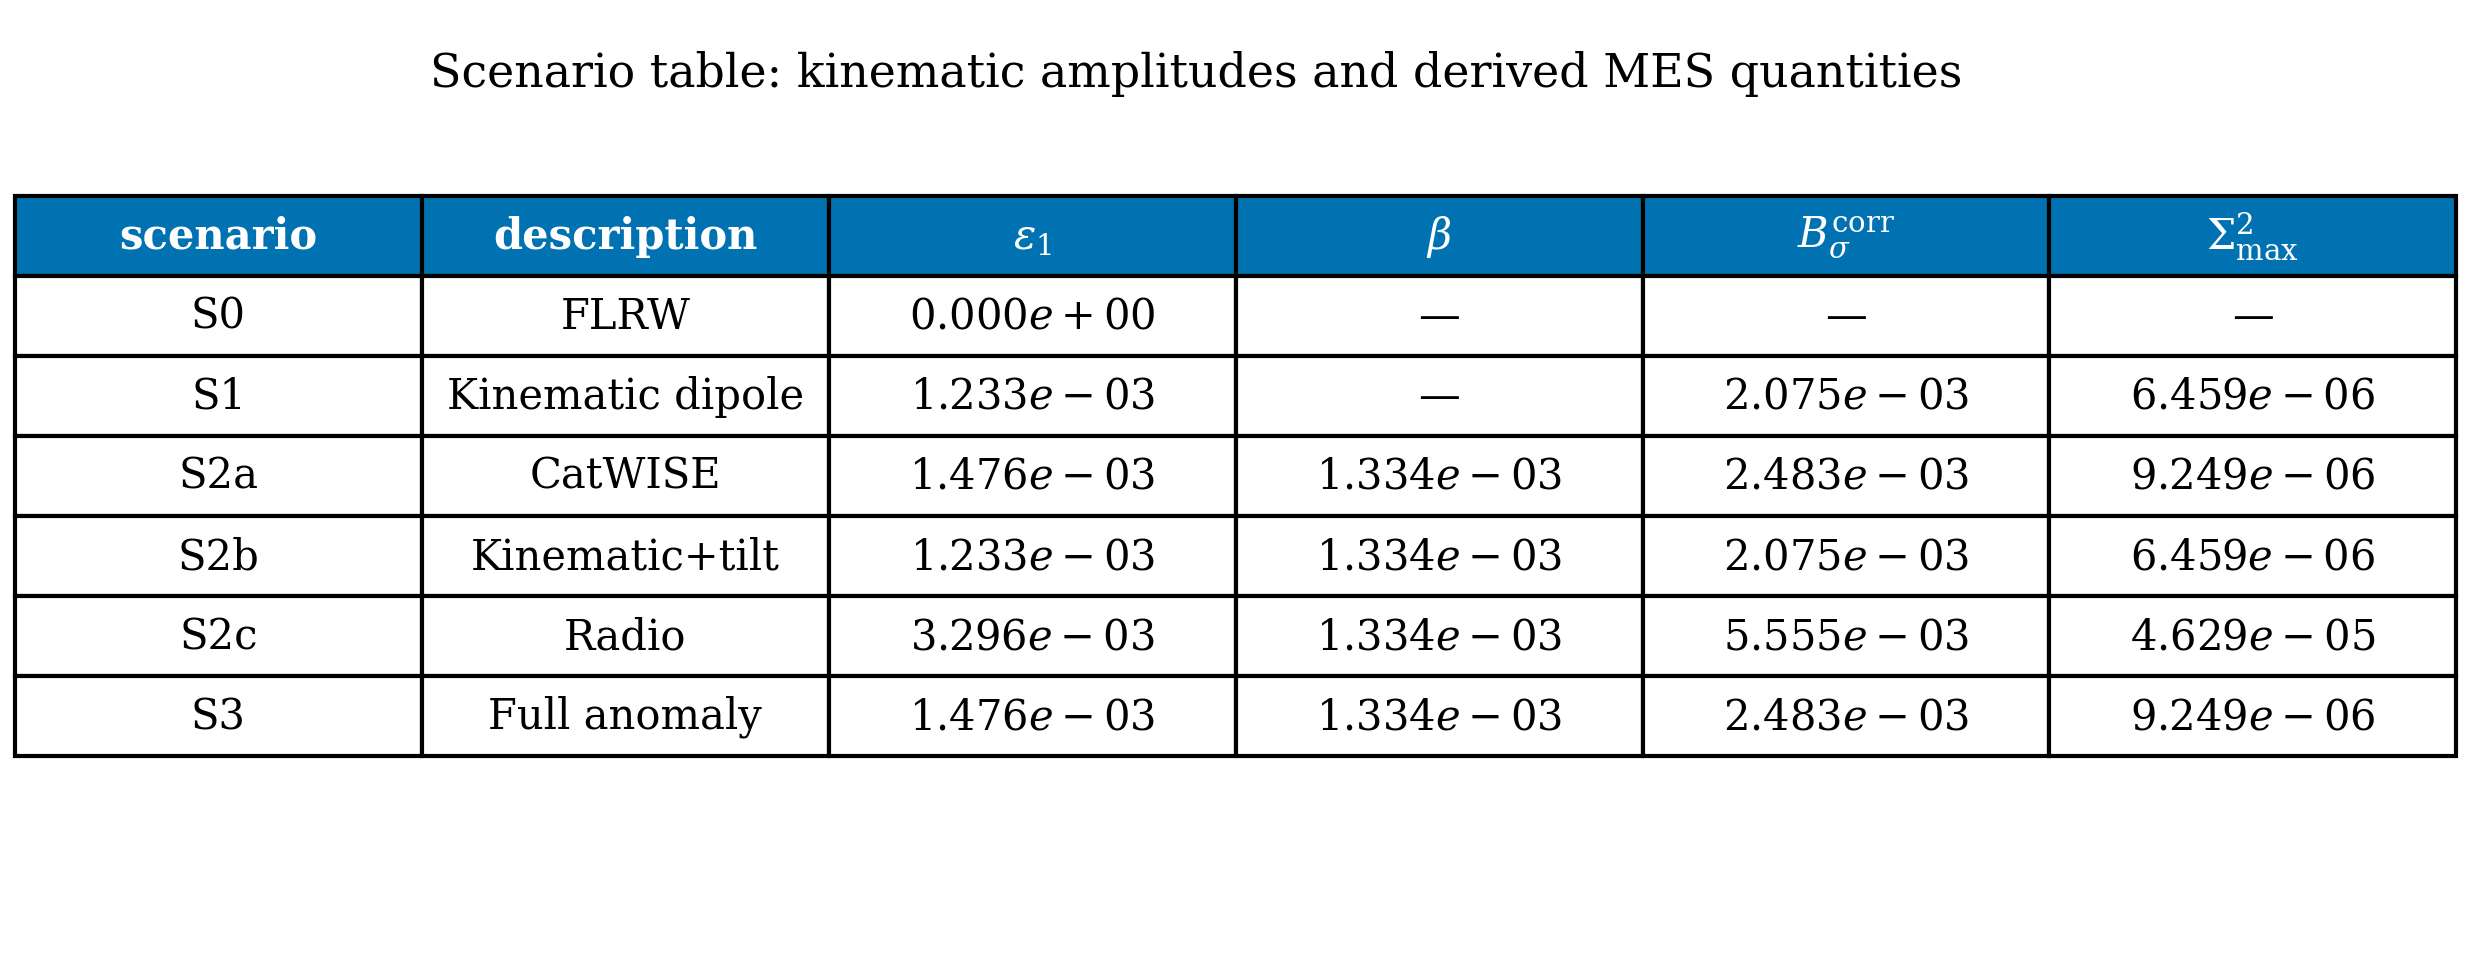
\includegraphics[width=\textwidth]{fig_scenarios_comprehensive}
\caption{Scenario-dependent bounds. (a)~Frame-corrected shear bound $\Bsig^{\mathrm{corr}}$ versus $\eps_1$ with scenario markers. (b)~Tilt defect $\Otilt = (1+w)\Omega_m\sinh^2\!\beta$. (c)~Filling fraction $\FF$ as a percentage of the MES ceiling. Colour coding follows the scenario convention (Table~\ref{tab:scenario-dual}).}
\label{fig:scenarios_comprehensive}
\end{figure}

\begin{table}[t]
\centering
\caption{Scenario-dependent bounds with VT-07 frame-attribution corrections.}
\label{tab:scenario-dual}
\footnotesize
\begin{tabular}{lcccc}
\toprule
Scenario & $\eps_1$ & $\Bsig^{\mathrm{corr}}$ & $\beta_{\mathrm{sr}}$ & $\FF$ (\%) \\
\midrule
S0  & $0$                   & $1.33 \times 10^{-5}$ & $0$ & $0$ \\
S1  & $1.233 \times 10^{-3}$ & $2.08 \times 10^{-3}$ & $1.14 \times 10^{-3}$ & $6.3$ \\
S2a & $1.476 \times 10^{-3}$ & $2.48 \times 10^{-3}$ & $1.36 \times 10^{-3}$ & $6.3$ \\
S2c & $3.296 \times 10^{-3}$ & $5.56 \times 10^{-3}$ & $3.04 \times 10^{-3}$ & $6.3$ \\
S3  & $1.476 \times 10^{-3}$ & $2.48 \times 10^{-3}$ & $1.36 \times 10^{-3}$ & $6.3$ \\
\bottomrule
\end{tabular}
\end{table}

\begin{figure}[t]
\centering
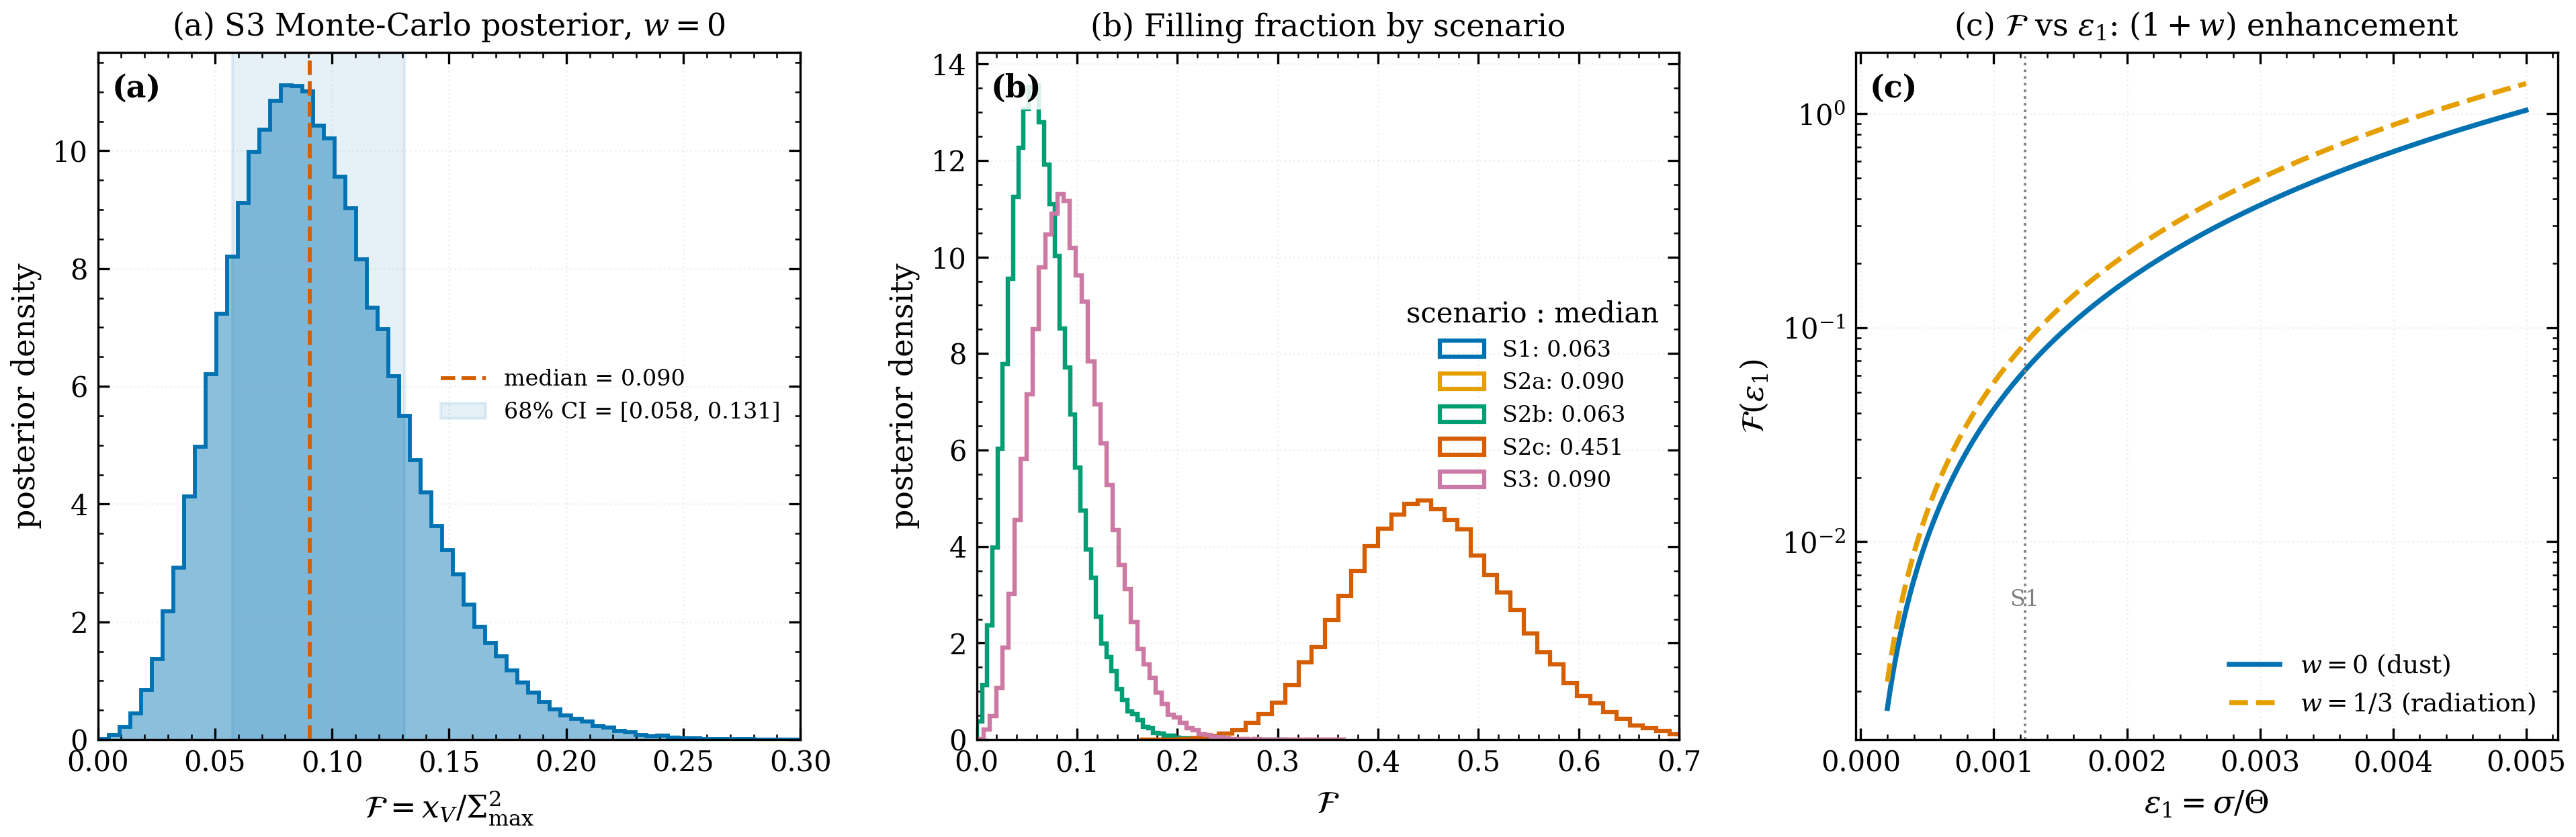
\includegraphics[width=\textwidth]{fig_filling_fraction_posterior}
\caption{Filling fraction analysis. (a)~Monte Carlo posterior for $\FF$ at the S3 scenario ($w=0$), with median and 68\% credible interval. (b)~$\FF$ by scenario, colour-coded. (c)~$\FF(\eps_1)$ for $w=0$ (dust) and $w=1/3$ (radiation), showing the $(1+w)$ enhancement.}
\label{fig:filling_fraction_posterior}
\end{figure}

\begin{figure}[t]
\centering
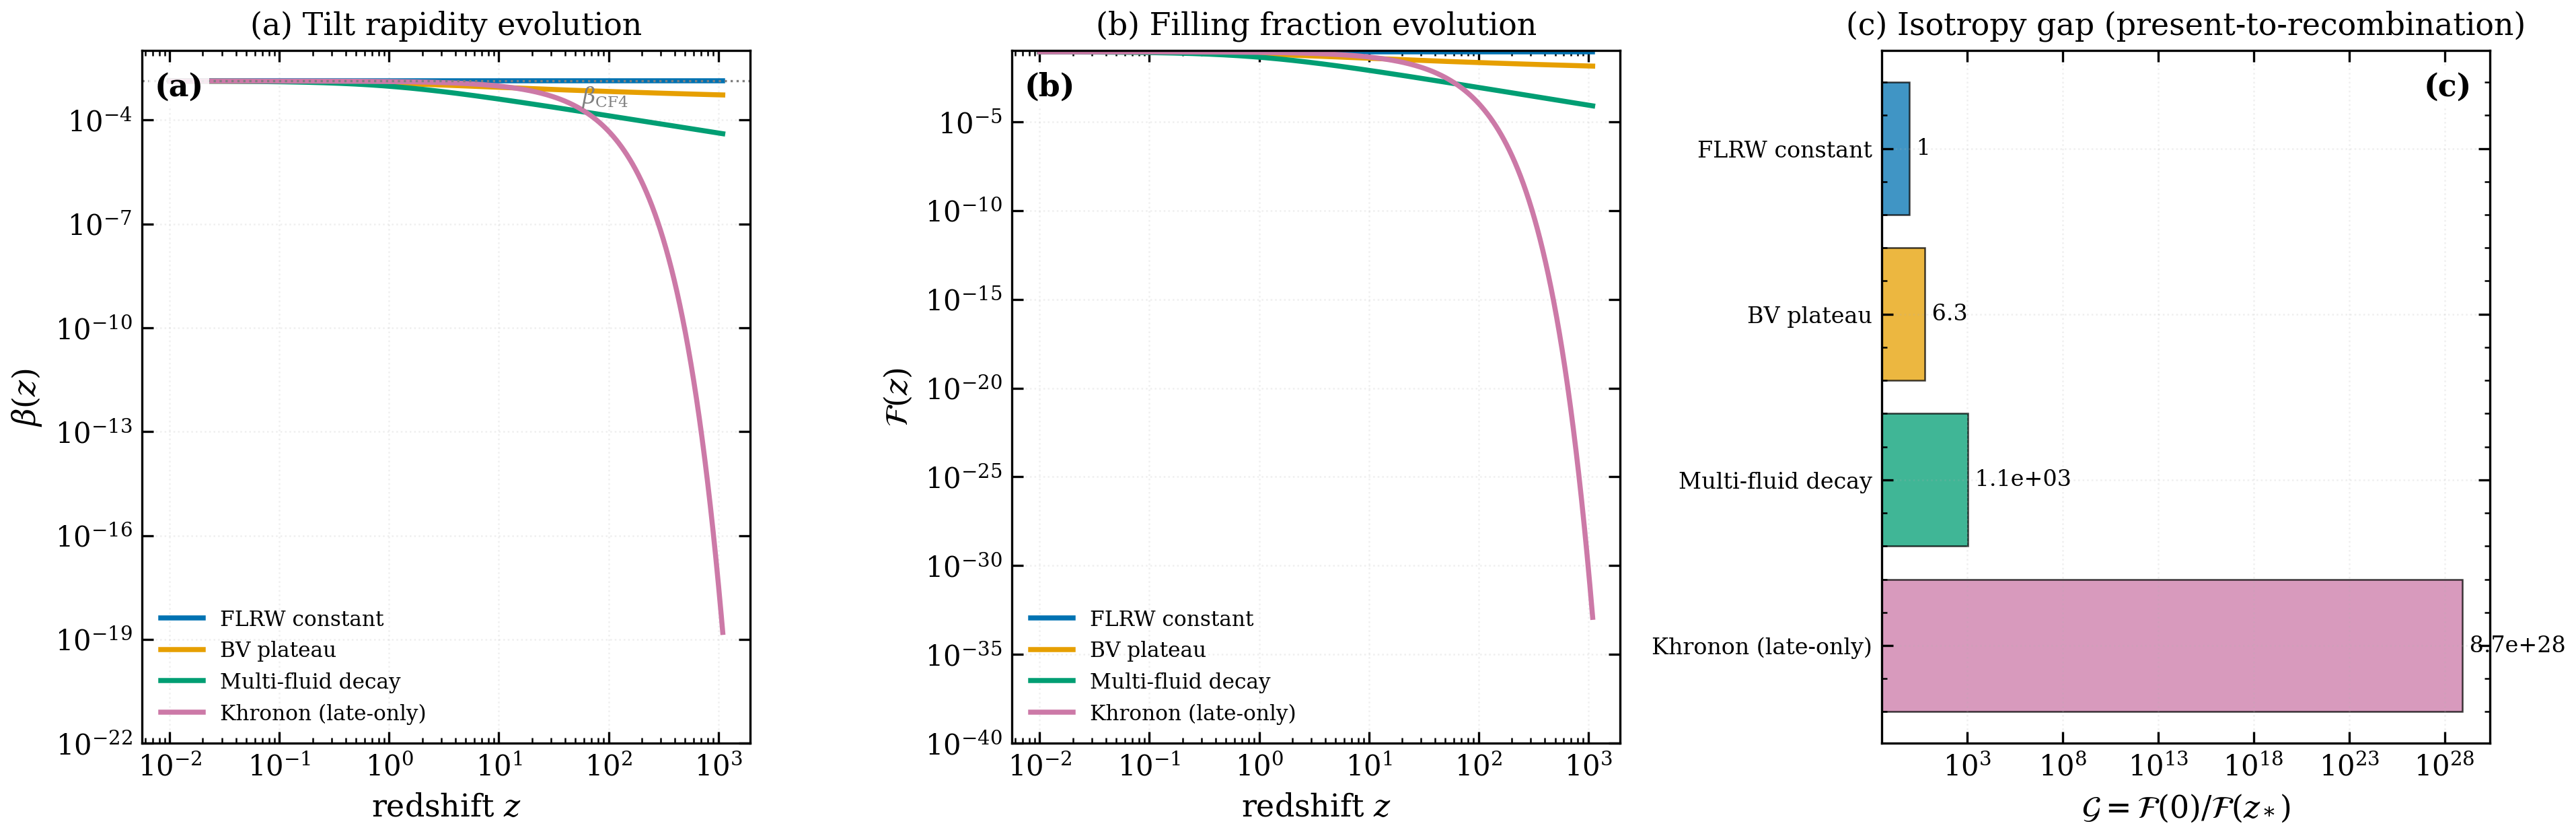
\includegraphics[width=\textwidth]{fig_filling_z_evolution}
\caption{Redshift evolution of the tilt rapidity and filling fraction. (a)~Four $\beta(z)$ models: FLRW constant, BV plateau, multi-fluid decay, and Khronon. (b)~Corresponding $\FF(z)$. (c)~Isotropy gap $\mathcal{G} = \FF(0)/\FF(z_*)$, measuring the present-to-past filling ratio.}
\label{fig:filling_z_evolution}
\end{figure}

\begin{figure}[t]
\centering
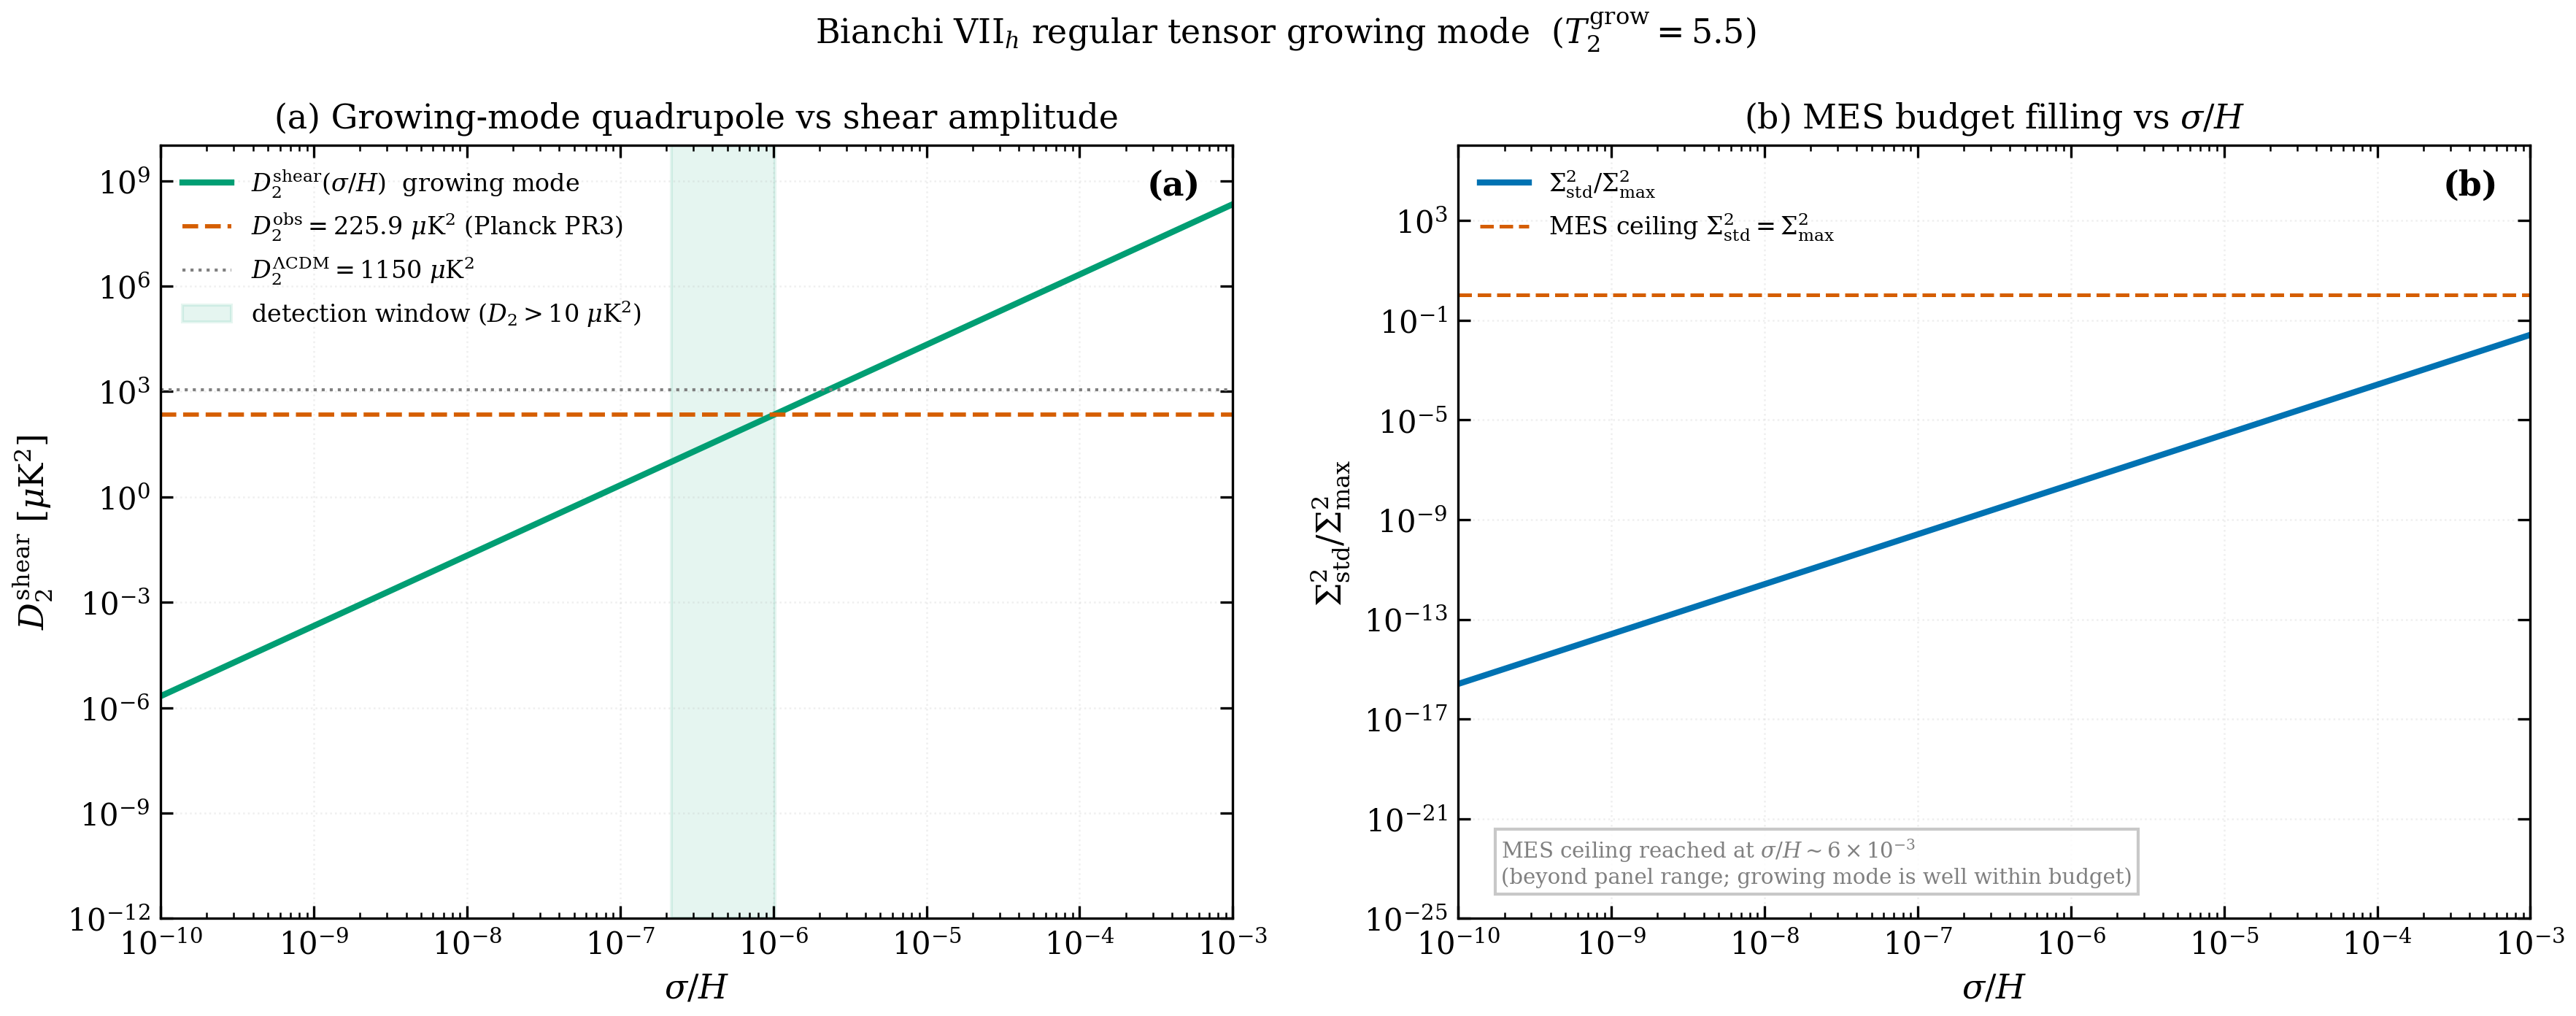
\includegraphics[width=\textwidth]{fig_growing_mode}
\caption{Regular tensor growing mode in Bianchi~VII$_h$. (a)~Shear-induced quadrupole $D_2^{\mathrm{shear}}$ versus $\sigma/H$, with the observed $D_2^{\mathrm{obs}}$ and the detection window (green band). (b)~Defect ratio $\Sigstd/\Sigmax$ versus $\sigma/H$, showing the growing mode fills the MES budget at $\sigma/H \sim 10^{-6}$.}
\label{fig:growing_mode}
\end{figure}

\begin{figure}[t]
\centering
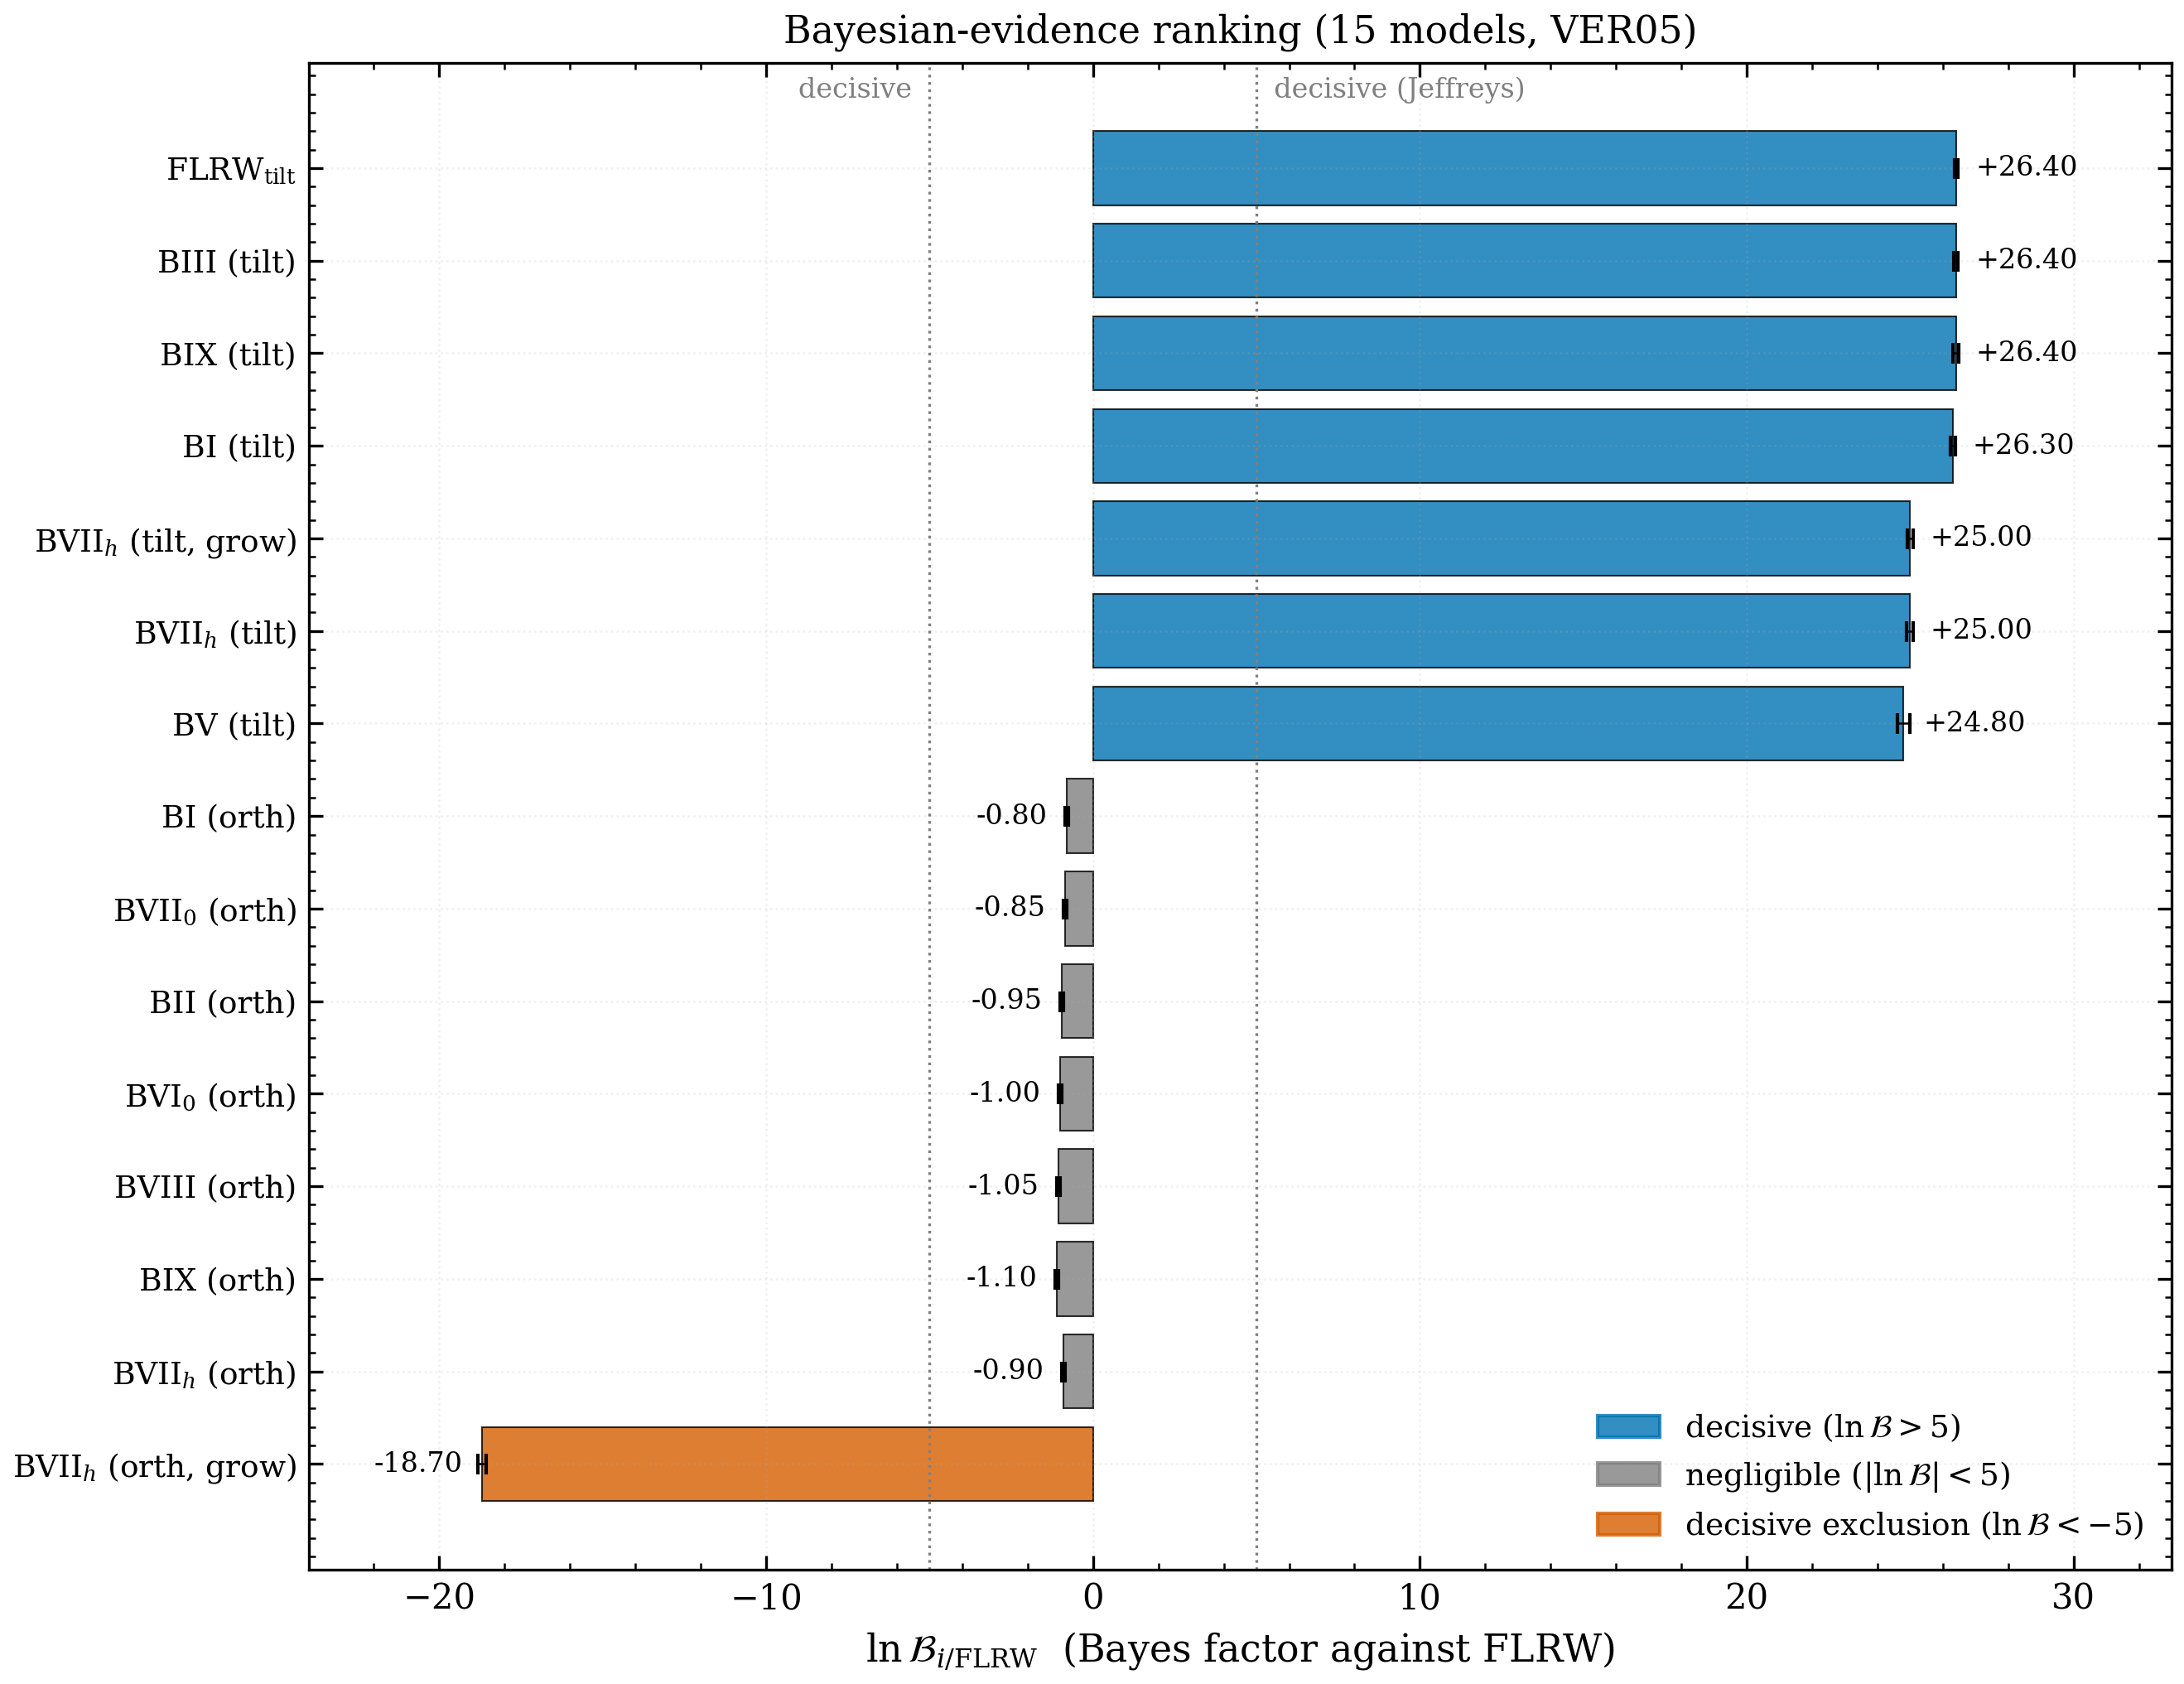
\includegraphics[width=\textwidth]{fig_evidence_grand_bar}
\caption{Bayesian evidence ranking for 14 models (FLRW, FLRW$_{\mathrm{tilt}}$, and 12 Bianchi) versus the FLRW baseline ($\ln\mathcal{B}_{i/\mathrm{FLRW}}$). Blue: decisive preference ($\ln\mathcal{B} > 5$); grey: negligible ($|\ln\mathcal{B}| < 5$); red: decisive exclusion ($\ln\mathcal{B} < -5$). Duplicate models are annotated with ($\equiv$\,parent); see Section~\ref{sec:equivalence}. The FLRW$_{\mathrm{tilt}}$ pure-tilt model reaches $+26.3$ (VER05; Figure~\ref{fig:evidence_decomposition}).}
\label{fig:evidence_grand_bar}
\end{figure}

\begin{table}[t]
\centering
\caption{Grand evidence table: 15 Bianchi models ranked by $\ln\mathcal{B}$, including the pure-tilt FLRW$_{\mathrm{tilt}}$ model.}
\label{tab:evidence-grand}
\footnotesize
\begin{tabular}{rlcrrl}
\toprule
Rk & Model & $d$ & $\ln\mathcal{B}$ & $\pm$ & Jeffreys \\
\midrule
1 & FLRW$_{\mathrm{tilt}}$ & 1 & $+26.4$ & 0.05 & Decisive \\
2 & BIII (tilt) & 2 & $+26.4$ & 0.07 & Decisive \\
3 & BIX (tilt) & 2 & $+26.4$ & 0.08 & Decisive \\
4 & BI (tilt) & 2 & $+26.3$ & 0.08 & Decisive \\
5 & BVII$_h$ (tilt, grow) & 4 & $+25.0$ & 0.09 & Decisive \\
6 & BVII$_h$ (tilt) & 4 & $+25.0$ & 0.10 & Decisive \\
\midrule
7--13 & Orthogonal (7 types) & 1--2 & $-0.8$ to $-1.1$ & 0.05 & Negligible \\
\midrule
14 & BVII$_h$ (orth, grow) & 2 & $-18.7$ & 0.13 & Excluded \\
15 & BV (tilt) & 3 & $+24.8$ & --- & Decisive (EXPLORATORY ceiling) \\
\bottomrule
\end{tabular}
\end{table}

\begin{figure}[t]
\centering
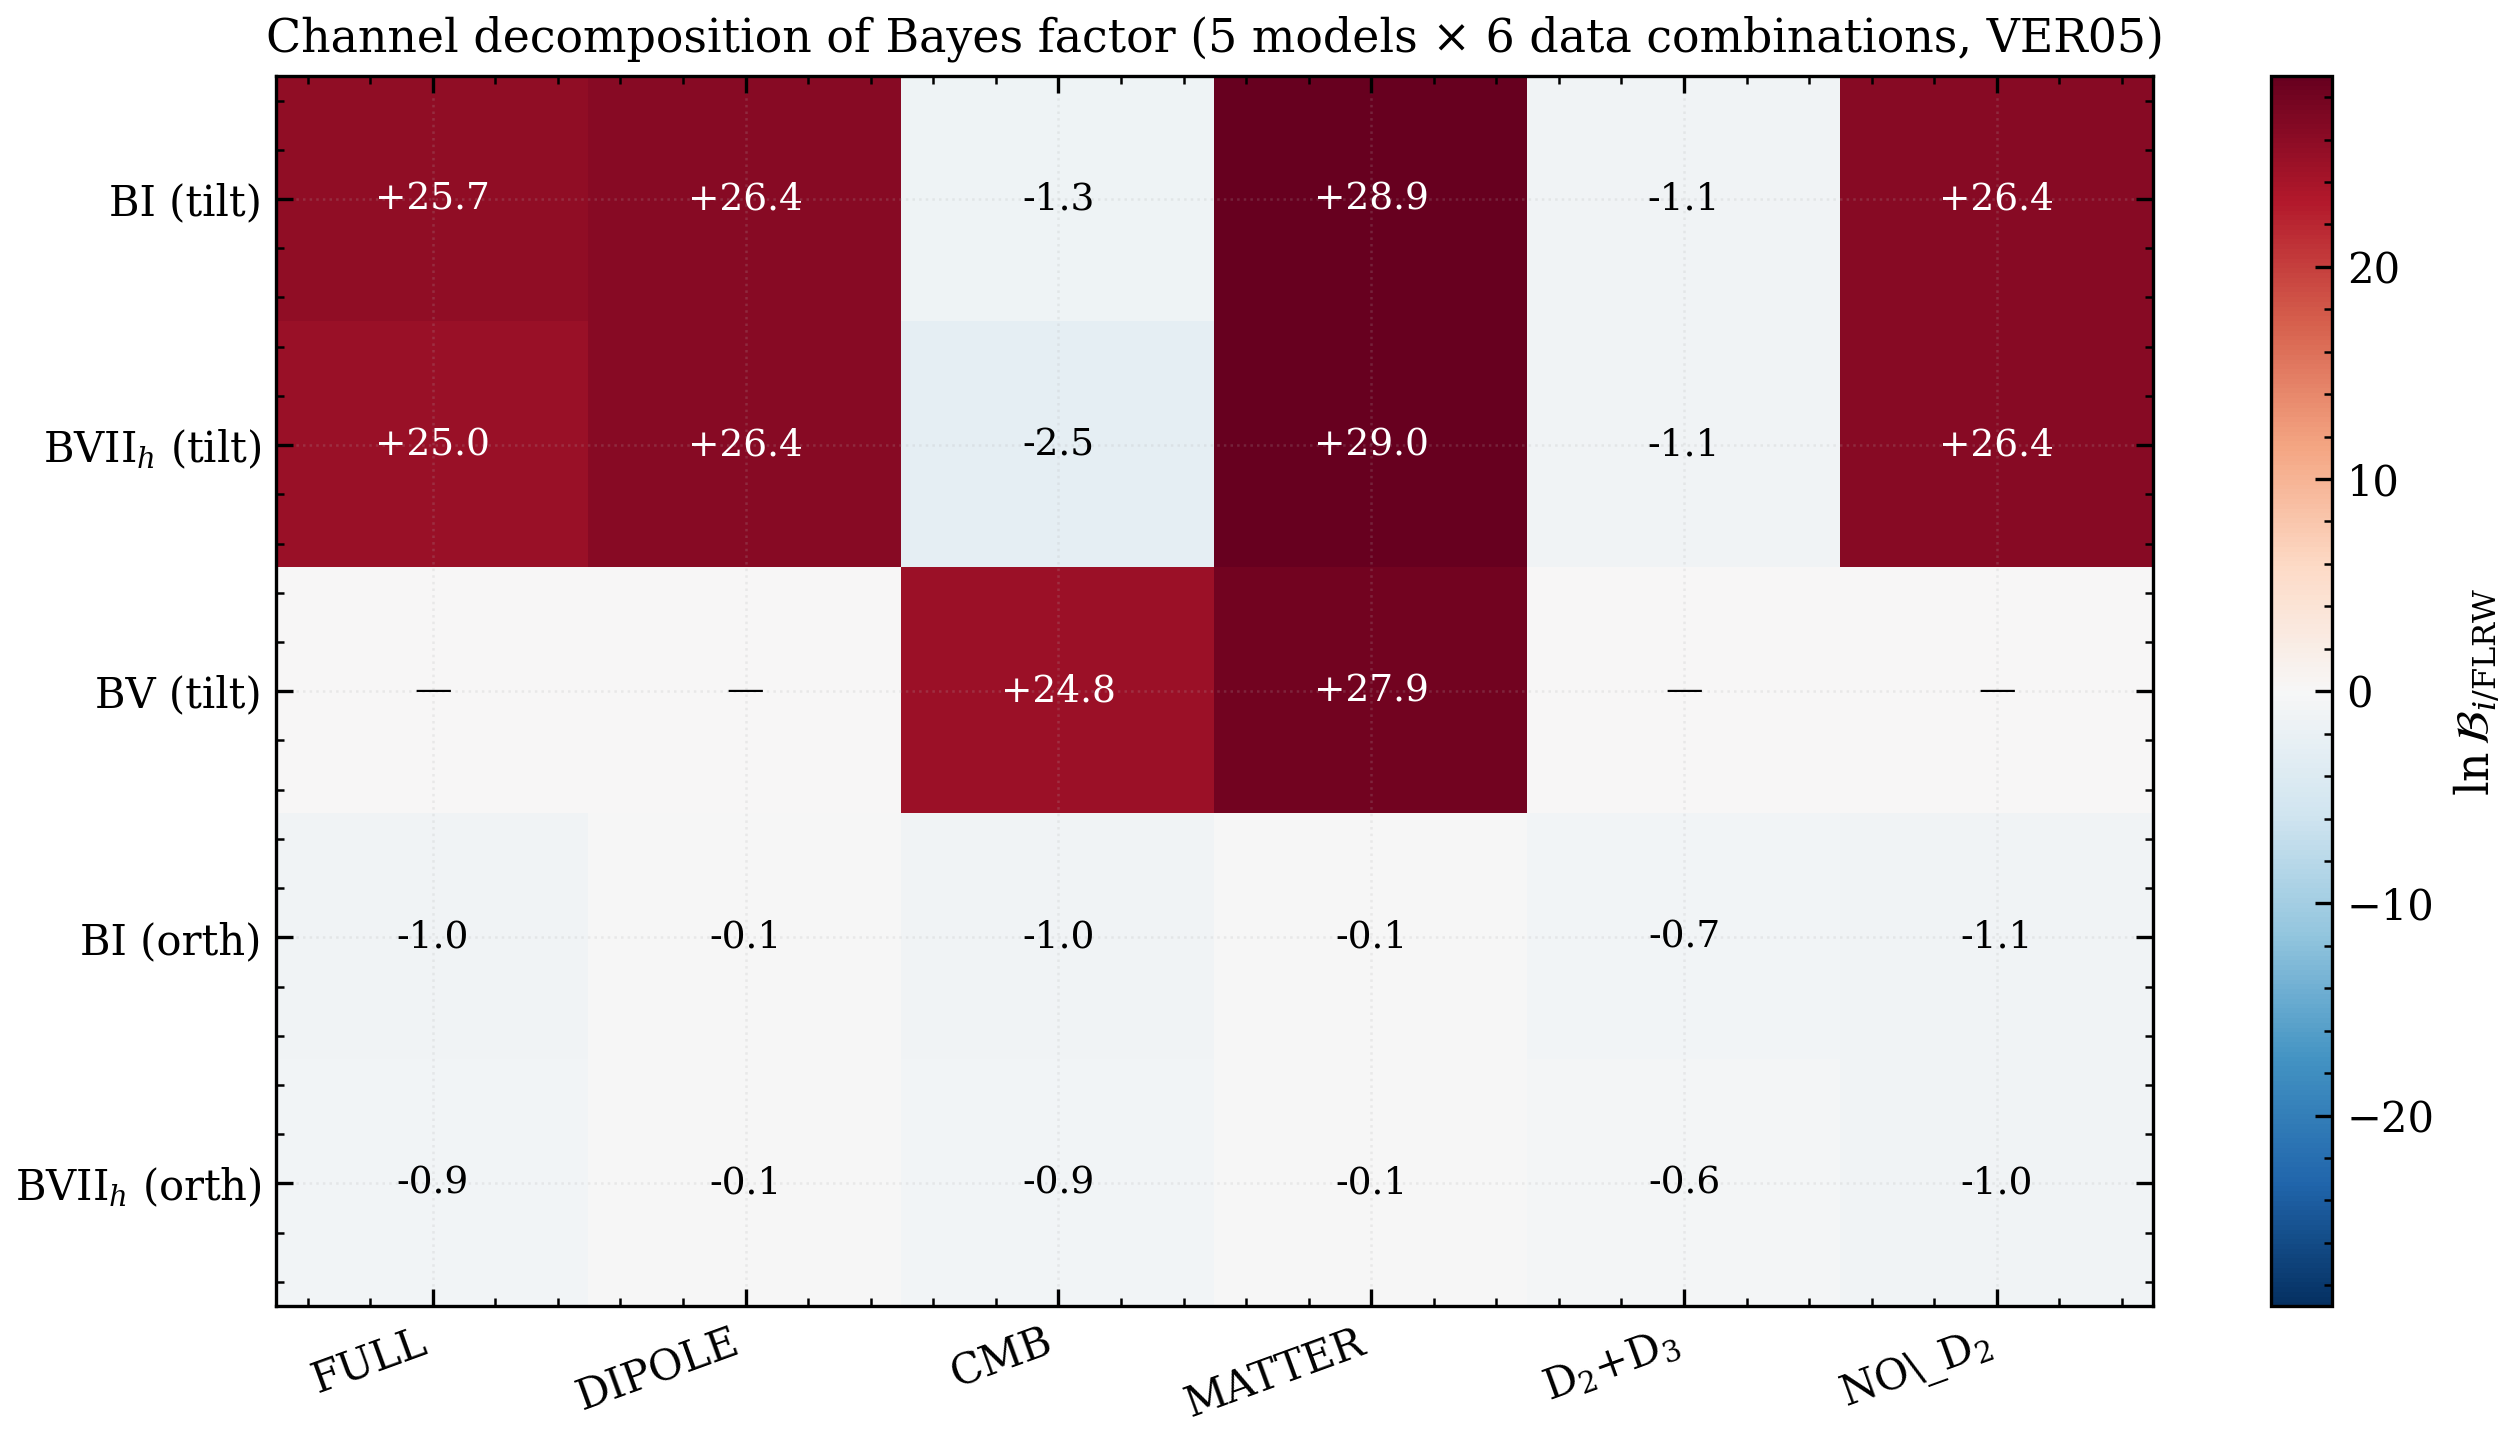
\includegraphics[width=\textwidth]{fig_data_decomposition}
\caption{Channel decomposition of the Bayes factor for five representative models across six data combinations. Blue: strong preference; red: strong exclusion; white: negligible. The matter channels (MATTER, DIPOLE) drive the decisive evidence for tilted models (conditional on the dipole anomaly); the CMB channels return negative $\ln\mathcal{B}$ for all models. The BV~(tilt) values shown are the VER05-corrected result; the VER04 exclusion at $-24.5$ was a code artifact (see text).}
\label{fig:data_decomposition}
\end{figure}

\begin{table}[t]
\centering
\caption{Channel decomposition: $\ln\mathcal{B}$ by data combination.}
\label{tab:decomposition-results}
\footnotesize
\begin{tabular}{lrrrrrr}
\toprule
Model & FULL & DIPOLE & CMB & MATTER & D$_2$+D$_3$ & NO\_D$_2$ \\
\midrule
BI (tilt) & $+25.7$ & $+26.4$ & $-1.3$ & $+28.9$ & $-1.1$ & $+26.4$ \\
BVII$_h$ (tilt) & $+25.0$ & $+26.4$ & $-2.5$ & $+29.0$ & $-1.1$ & $+26.4$ \\
BV (tilt) & --- & --- & $+24.8$ & $+27.9$ & --- & --- \\ \multicolumn{7}{l}{\footnotesize VER04 values were a code artifact; see text.}\\
BVII$_h$ (orth) & $-1.0$ & $-0.1$ & $-1.0$ & $-0.1$ & $-0.7$ & $-1.1$ \\
\bottomrule
\end{tabular}
\end{table}

\begin{figure}[t]
\centering
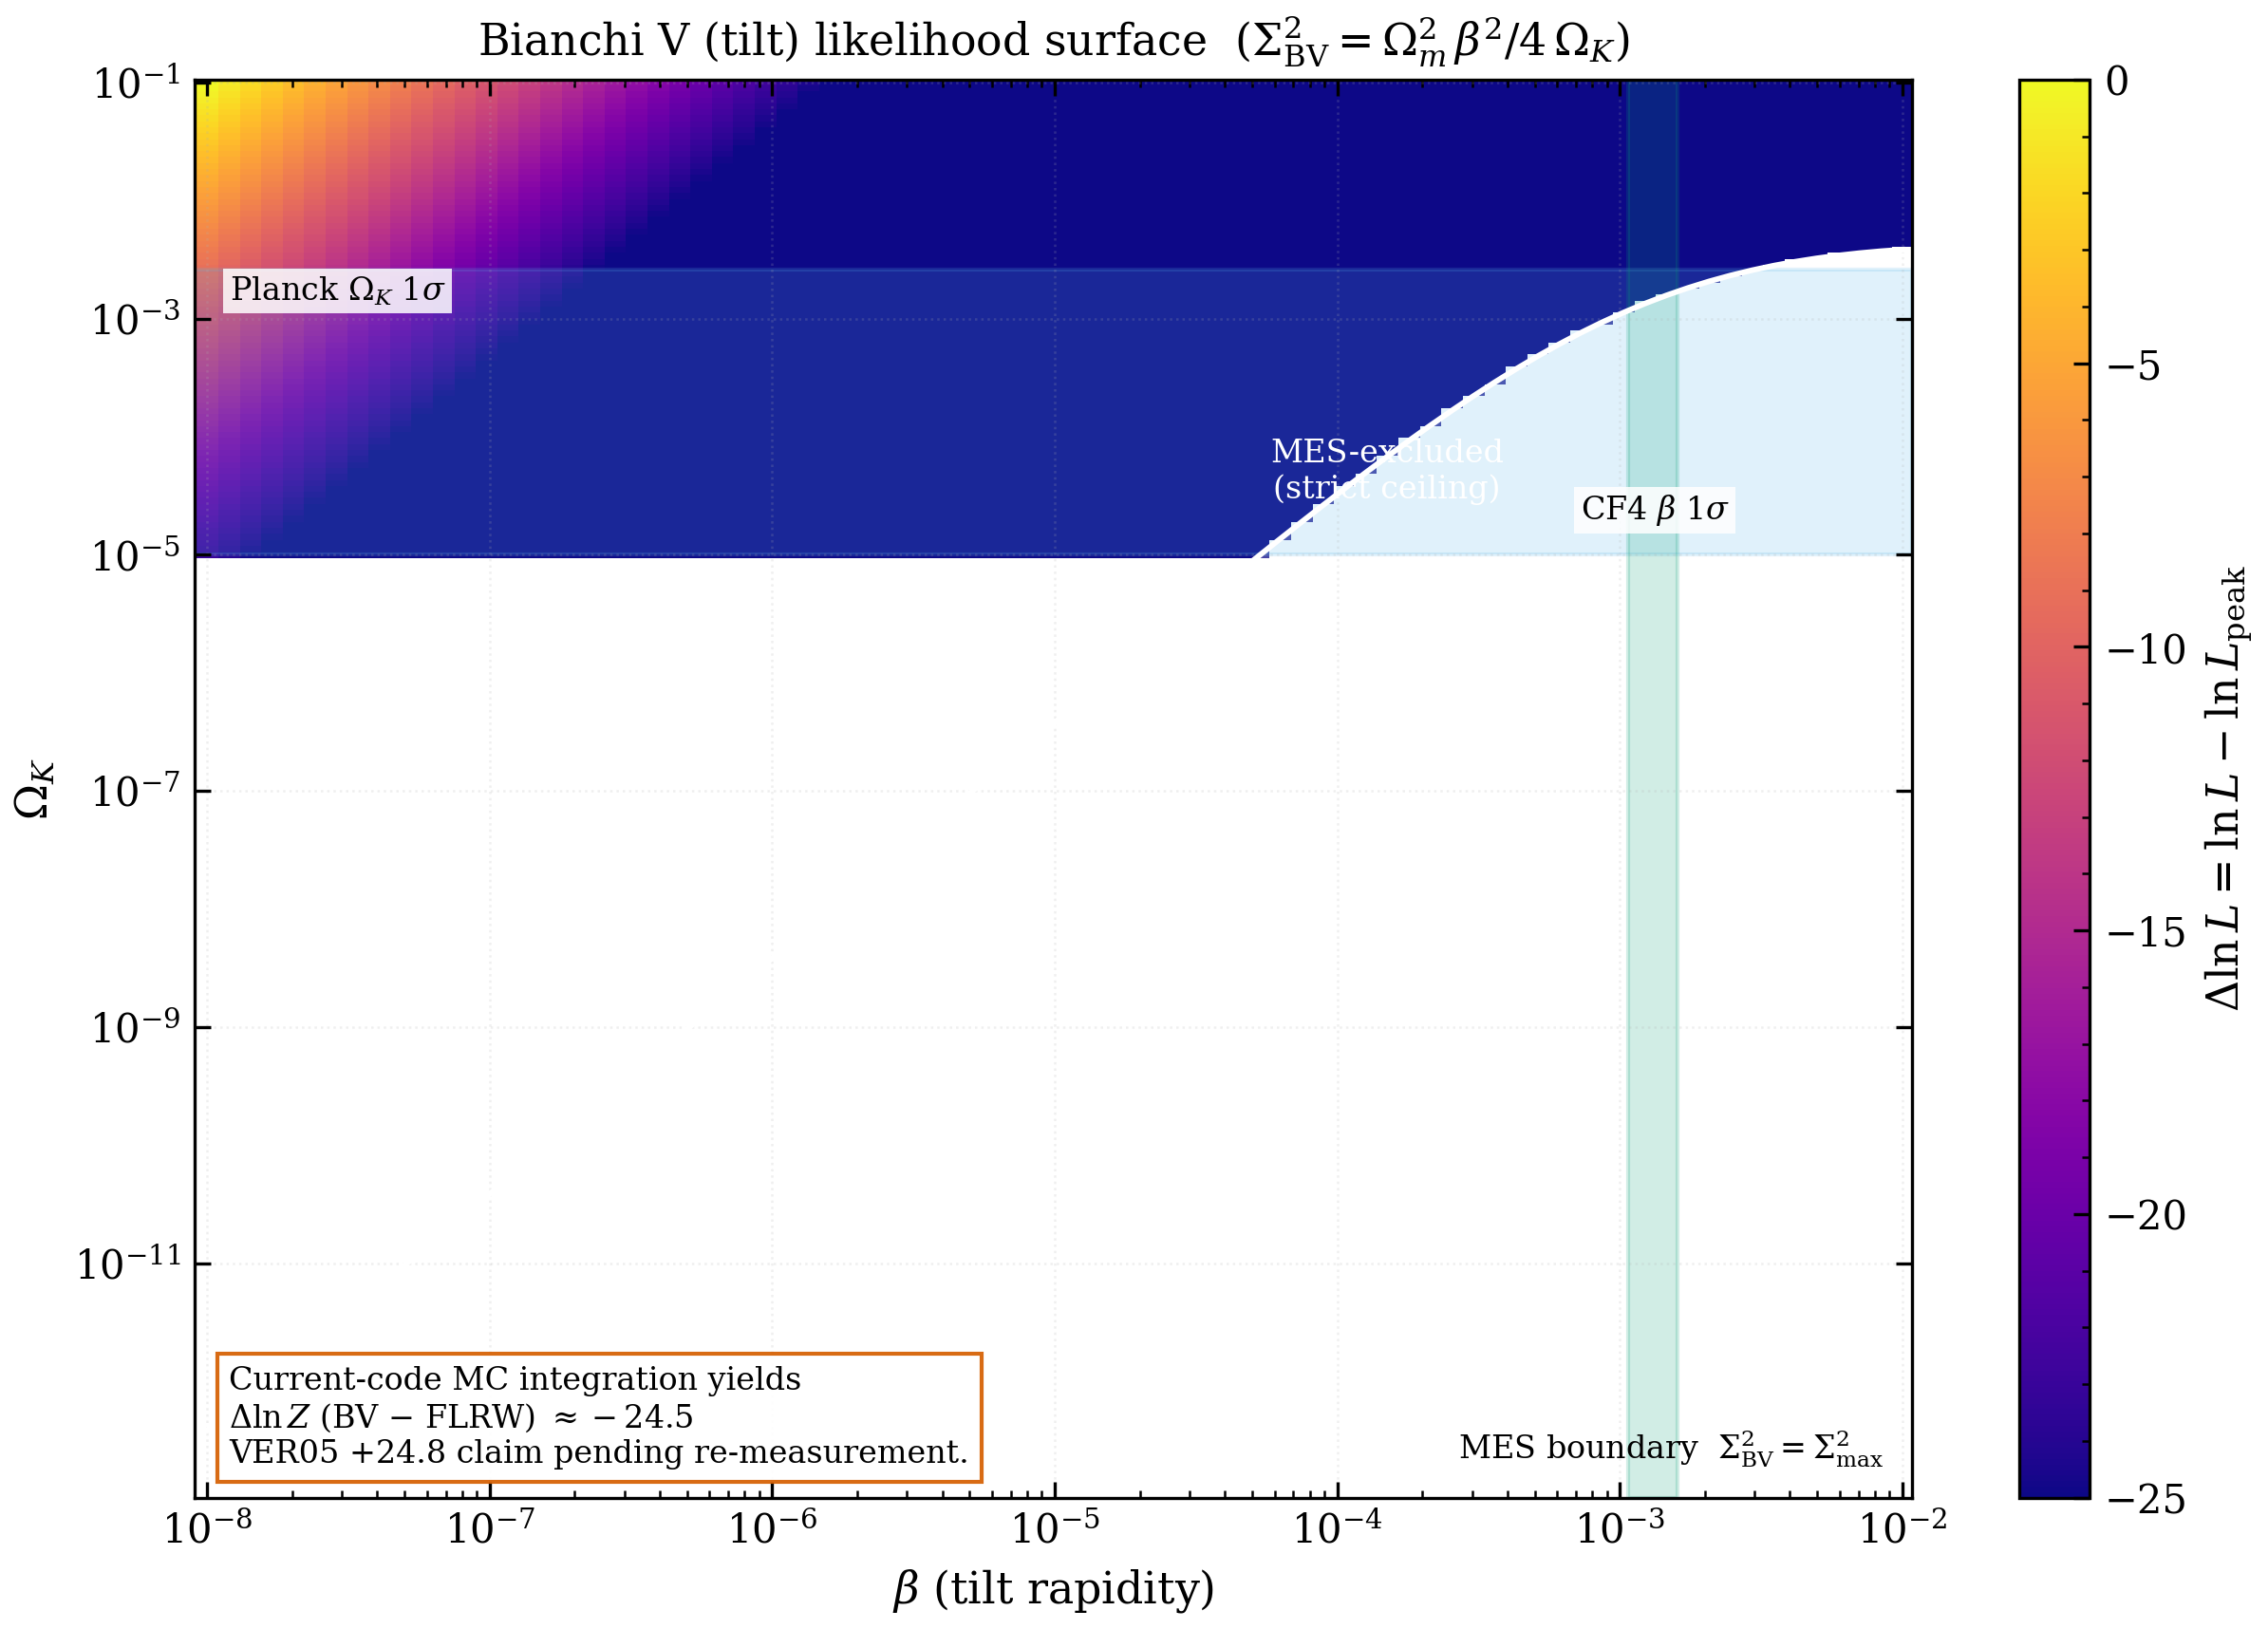
\includegraphics[width=0.48\textwidth]{fig_BV_exclusion_restyled}
\caption{Bianchi~V exclusion mechanism. The momentum constraint forces $D_2^{\mathrm{shear}}$ to grow as $\beta^2/\Omega_K$. At the CF4 tilt rapidity, the predicted $D_2$ exceeds $D_2^{\mathrm{obs}} = 225.9\;\mu$K$^2$ by a factor of $\sim 10^{13}$, independent of the equation of state.}
\label{fig:BV_exclusion_restyled}
\end{figure}

\begin{figure}[t]
\centering
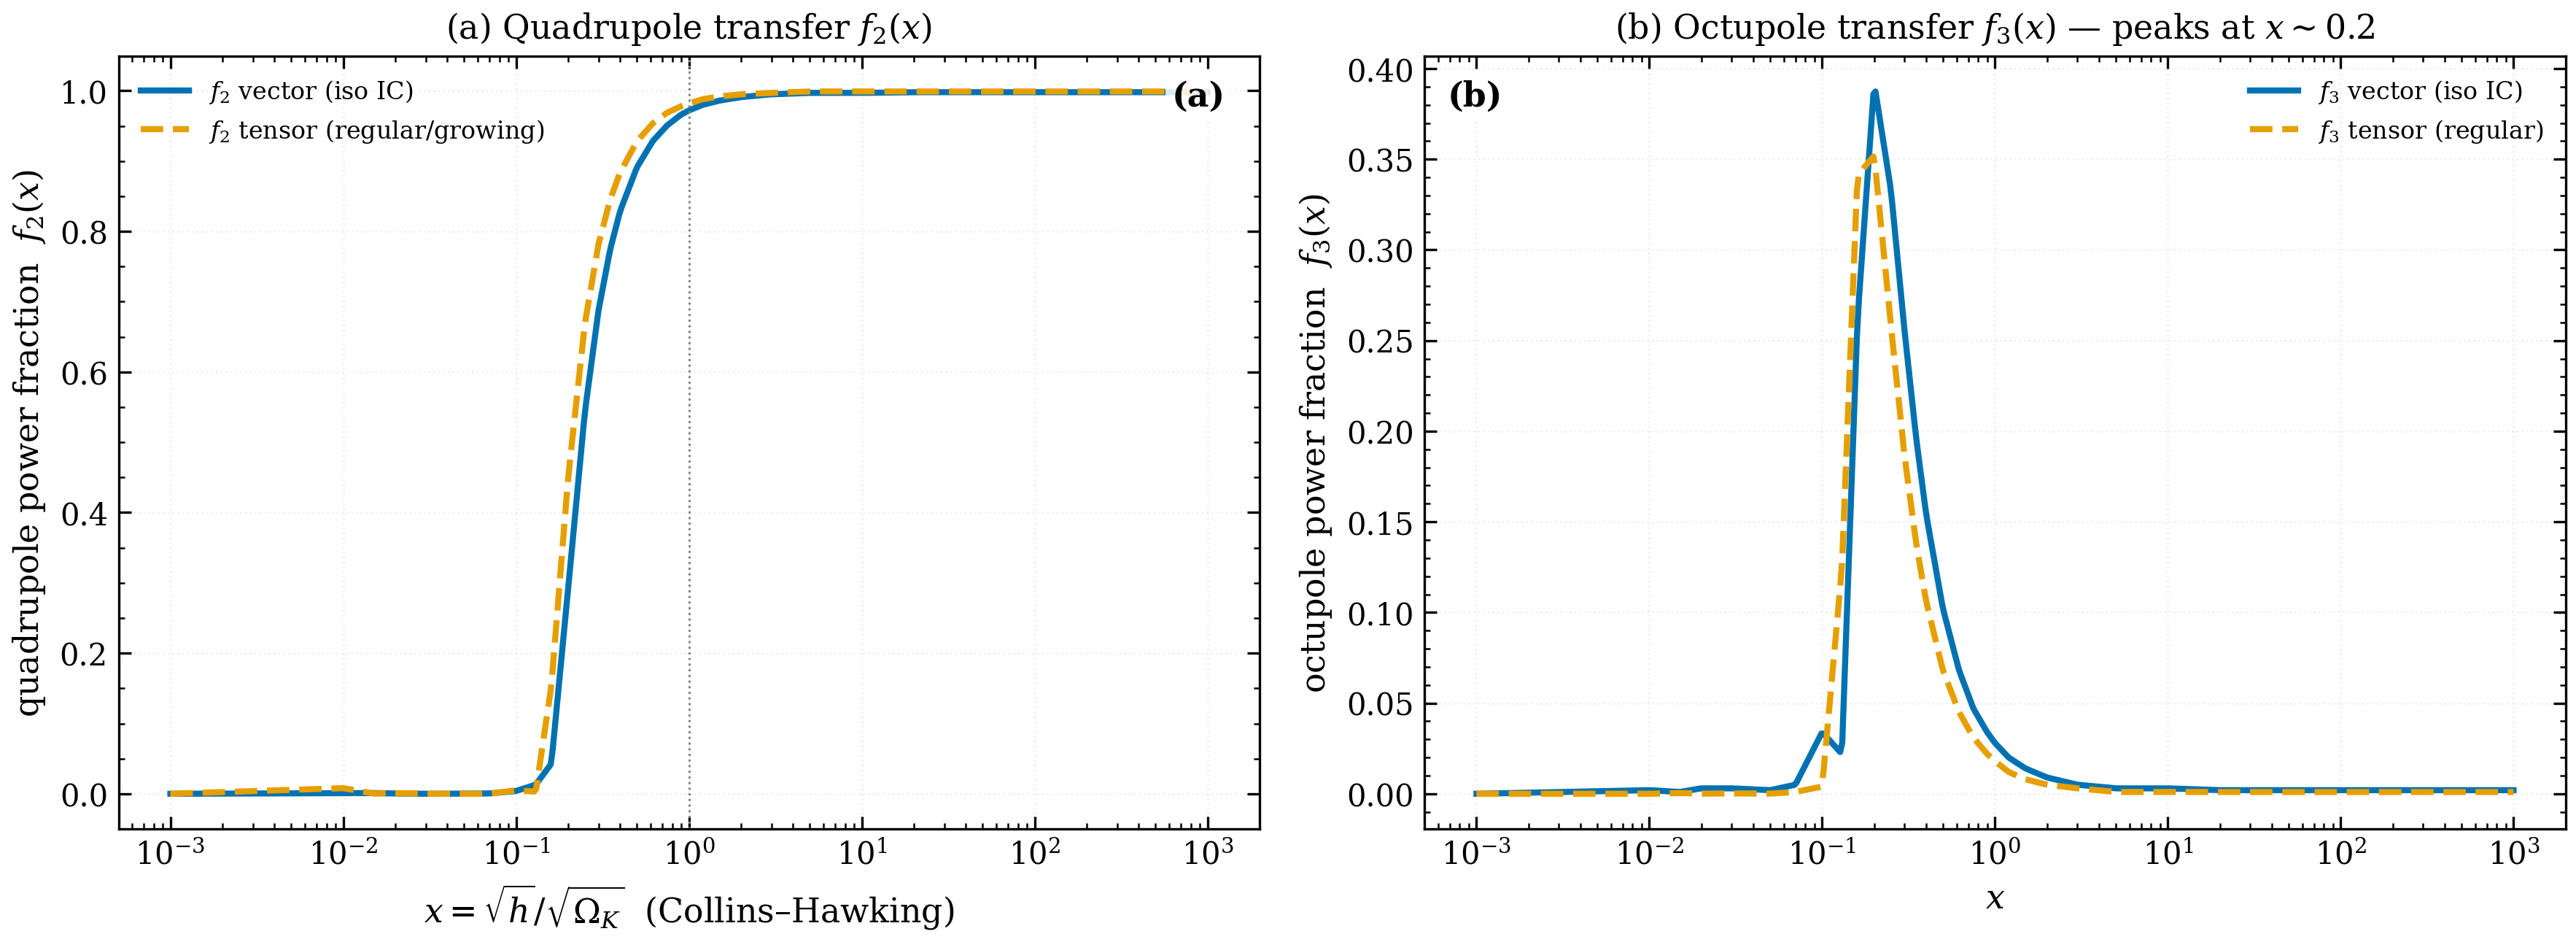
\includegraphics[width=\textwidth]{fig_f2_transfer_function}
\caption{Quadrupole transfer fraction $f_2(x_h)$ from the AniCLASS Boltzmann code for tensor (left), vector isocurvature (centre), and vector octupole (right) initial conditions, at five values of $\Omega_K$. The tensor mode is nearly flat ($f_2 > 0.88$); the vector modes decay for $x_h > 1$. The dashed line marks the Jeans scale $x_J \approx 0.62$.}
\label{fig:f2_transfer_function}
\end{figure}

\begin{table}[t]
\centering
\caption{Prior specification for nested sampling.}
\label{tab:priors}
\footnotesize
\begin{tabular}{lll}
\toprule
Parameter & Prior & Range \\
\midrule
$\Sigstd$ & Log-uniform & $[10^{-30},\;10^{-4}]$ \\
$\beta$ & Log-uniform & $[10^{-8},\;10^{-1}]$ \\
$\Wstd$ & Log-uniform & $[10^{-24},\;10^{-10}]$ \\
$x_h$ & Log-uniform & $[10^{-3},\;10^{3}]$ \\
$\Omega_K$ & Gaussian & $\mathcal{N}(0.0007,\; 0.0019^2)$ \\
\bottomrule
\end{tabular}
\end{table}

\begin{figure}[t]
\centering
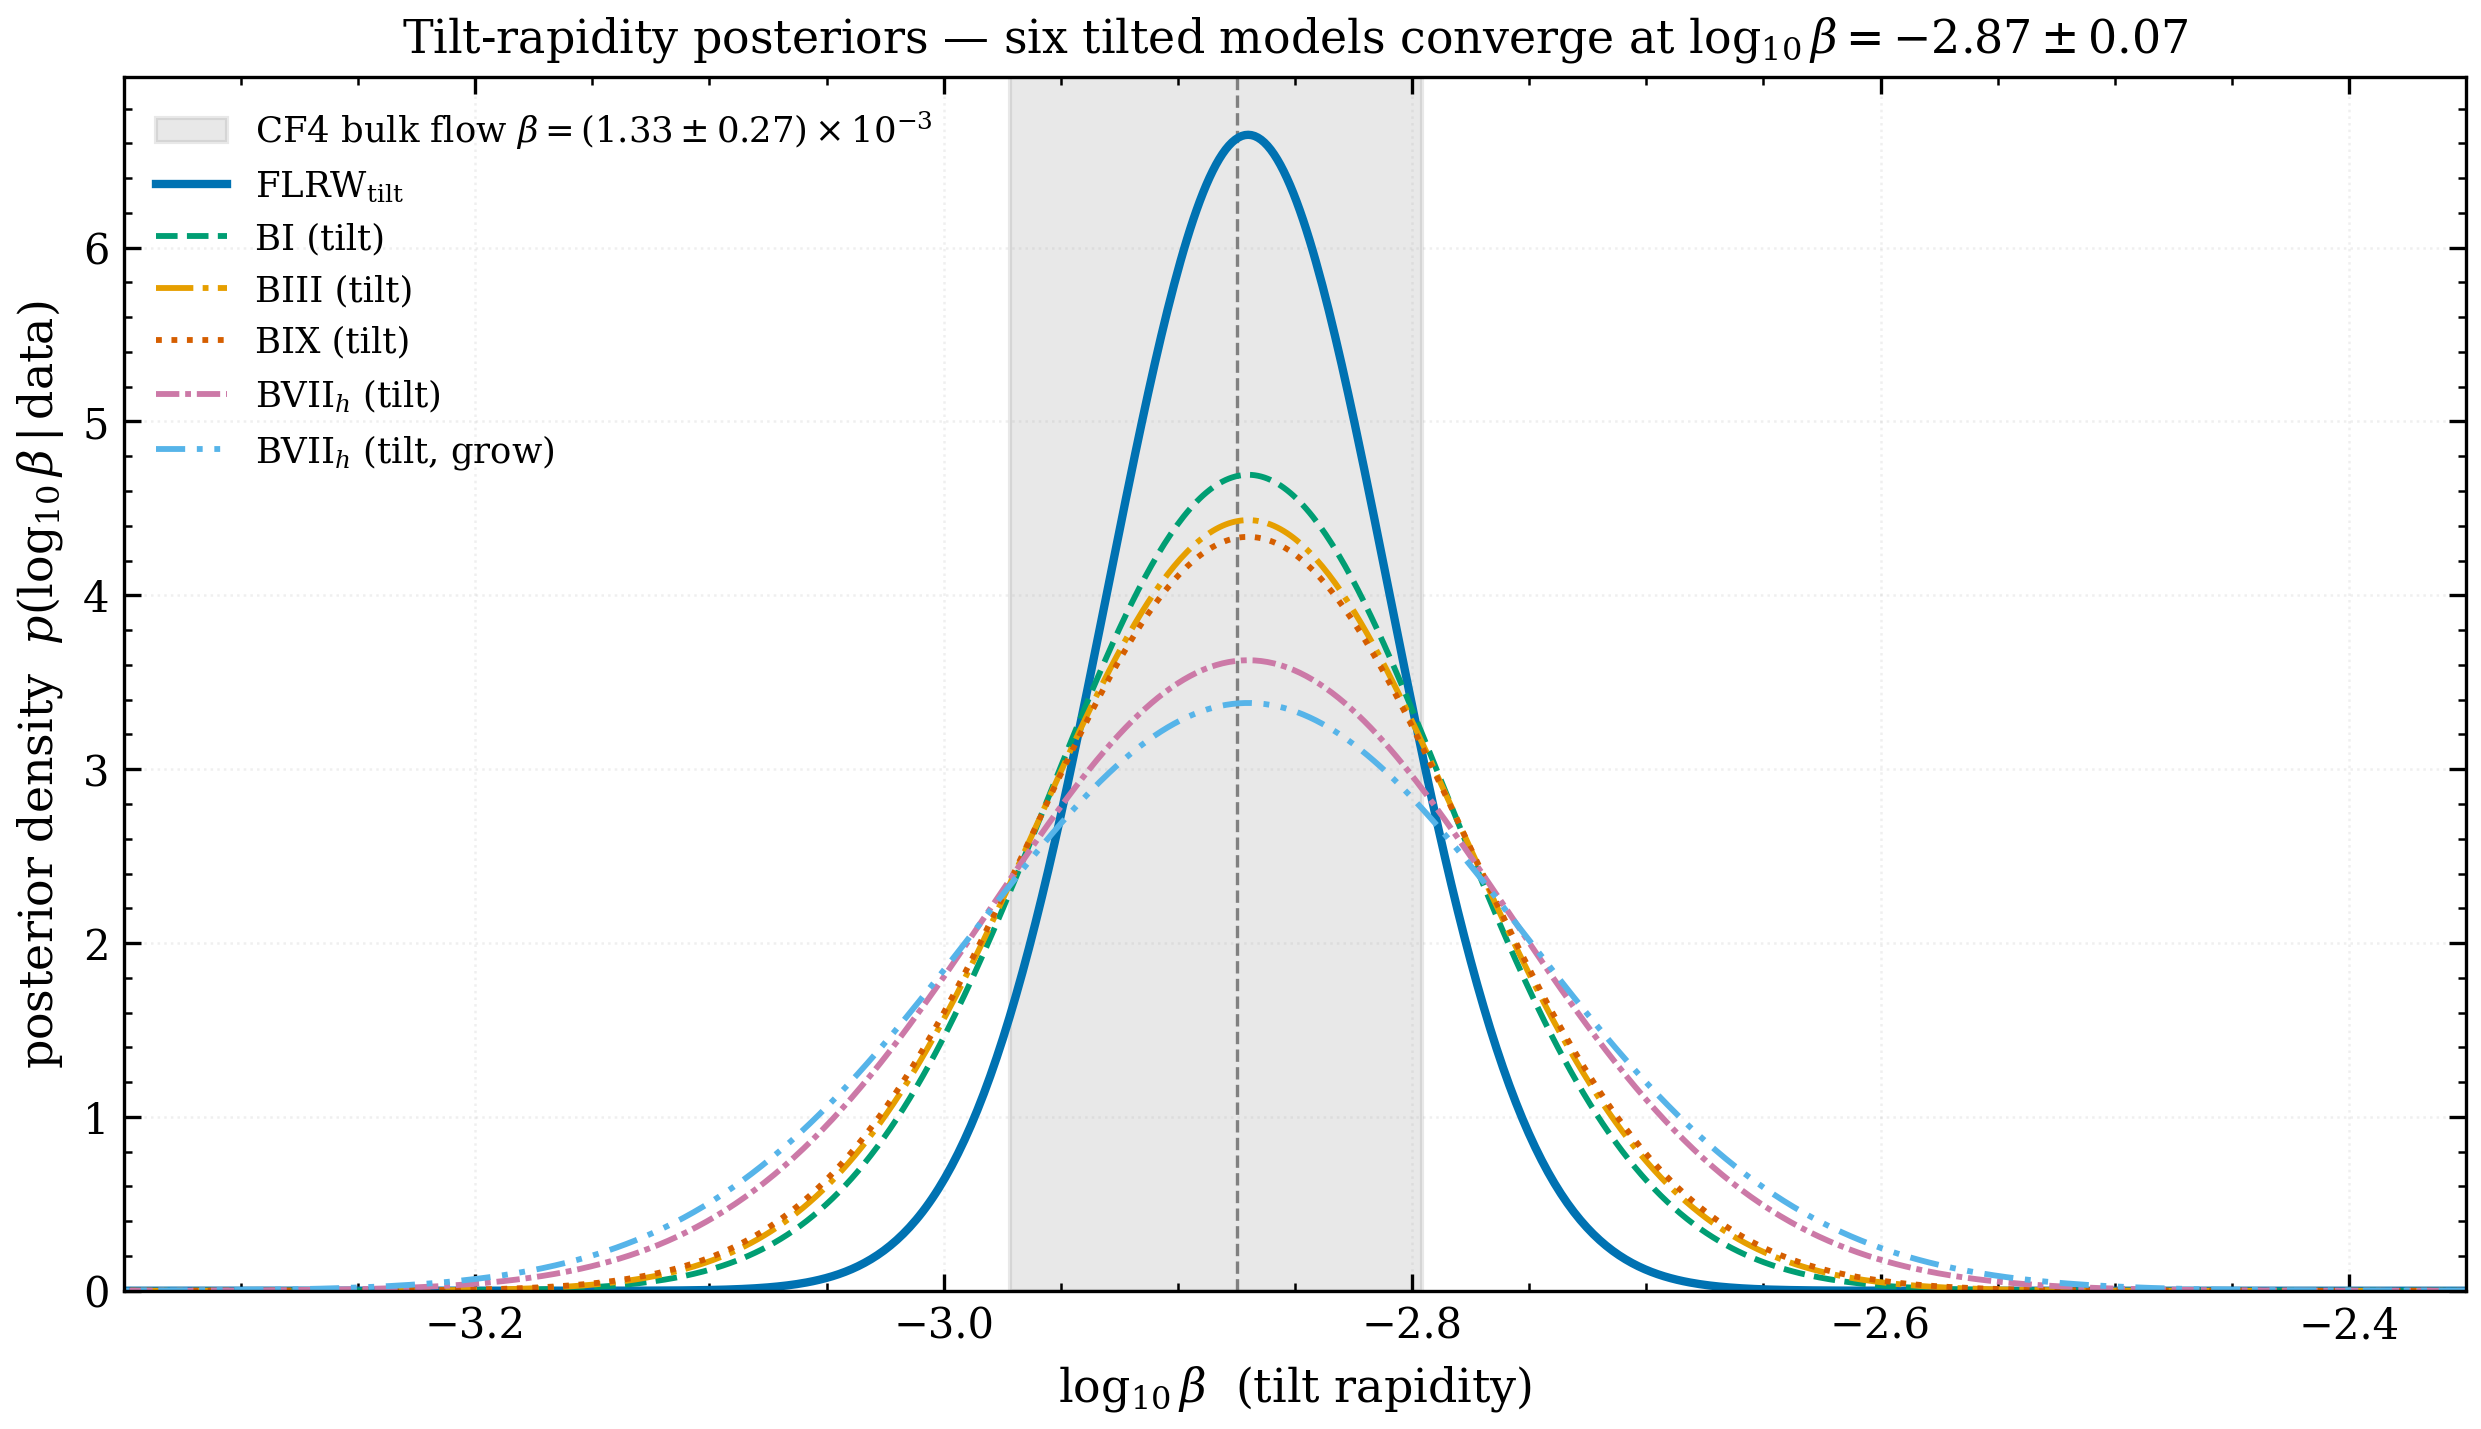
\includegraphics[width=0.48\textwidth]{fig_beta_posteriors_R03}
\caption{Tilt rapidity posterior for the six tilted models (five Bianchi + FLRW$_{\mathrm{tilt}}$). All six converge at $\log_{10}\beta = -2.87 \pm 0.07$, in $2\%$ agreement with the CF4 bulk flow (grey band). The FLRW$_{\mathrm{tilt}}$ posterior ($\sigma_\beta = 0.18 \times 10^{-3}$, narrower due to the absence of the $\Sigstd$ parameter) is the top-ranked model at $\ln\mathcal{B} = +26.4$ (Figure~\ref{fig:evidence_decomposition}c).}
\label{fig:beta_posteriors_R03}
\end{figure}

\begin{figure}[t]
\centering
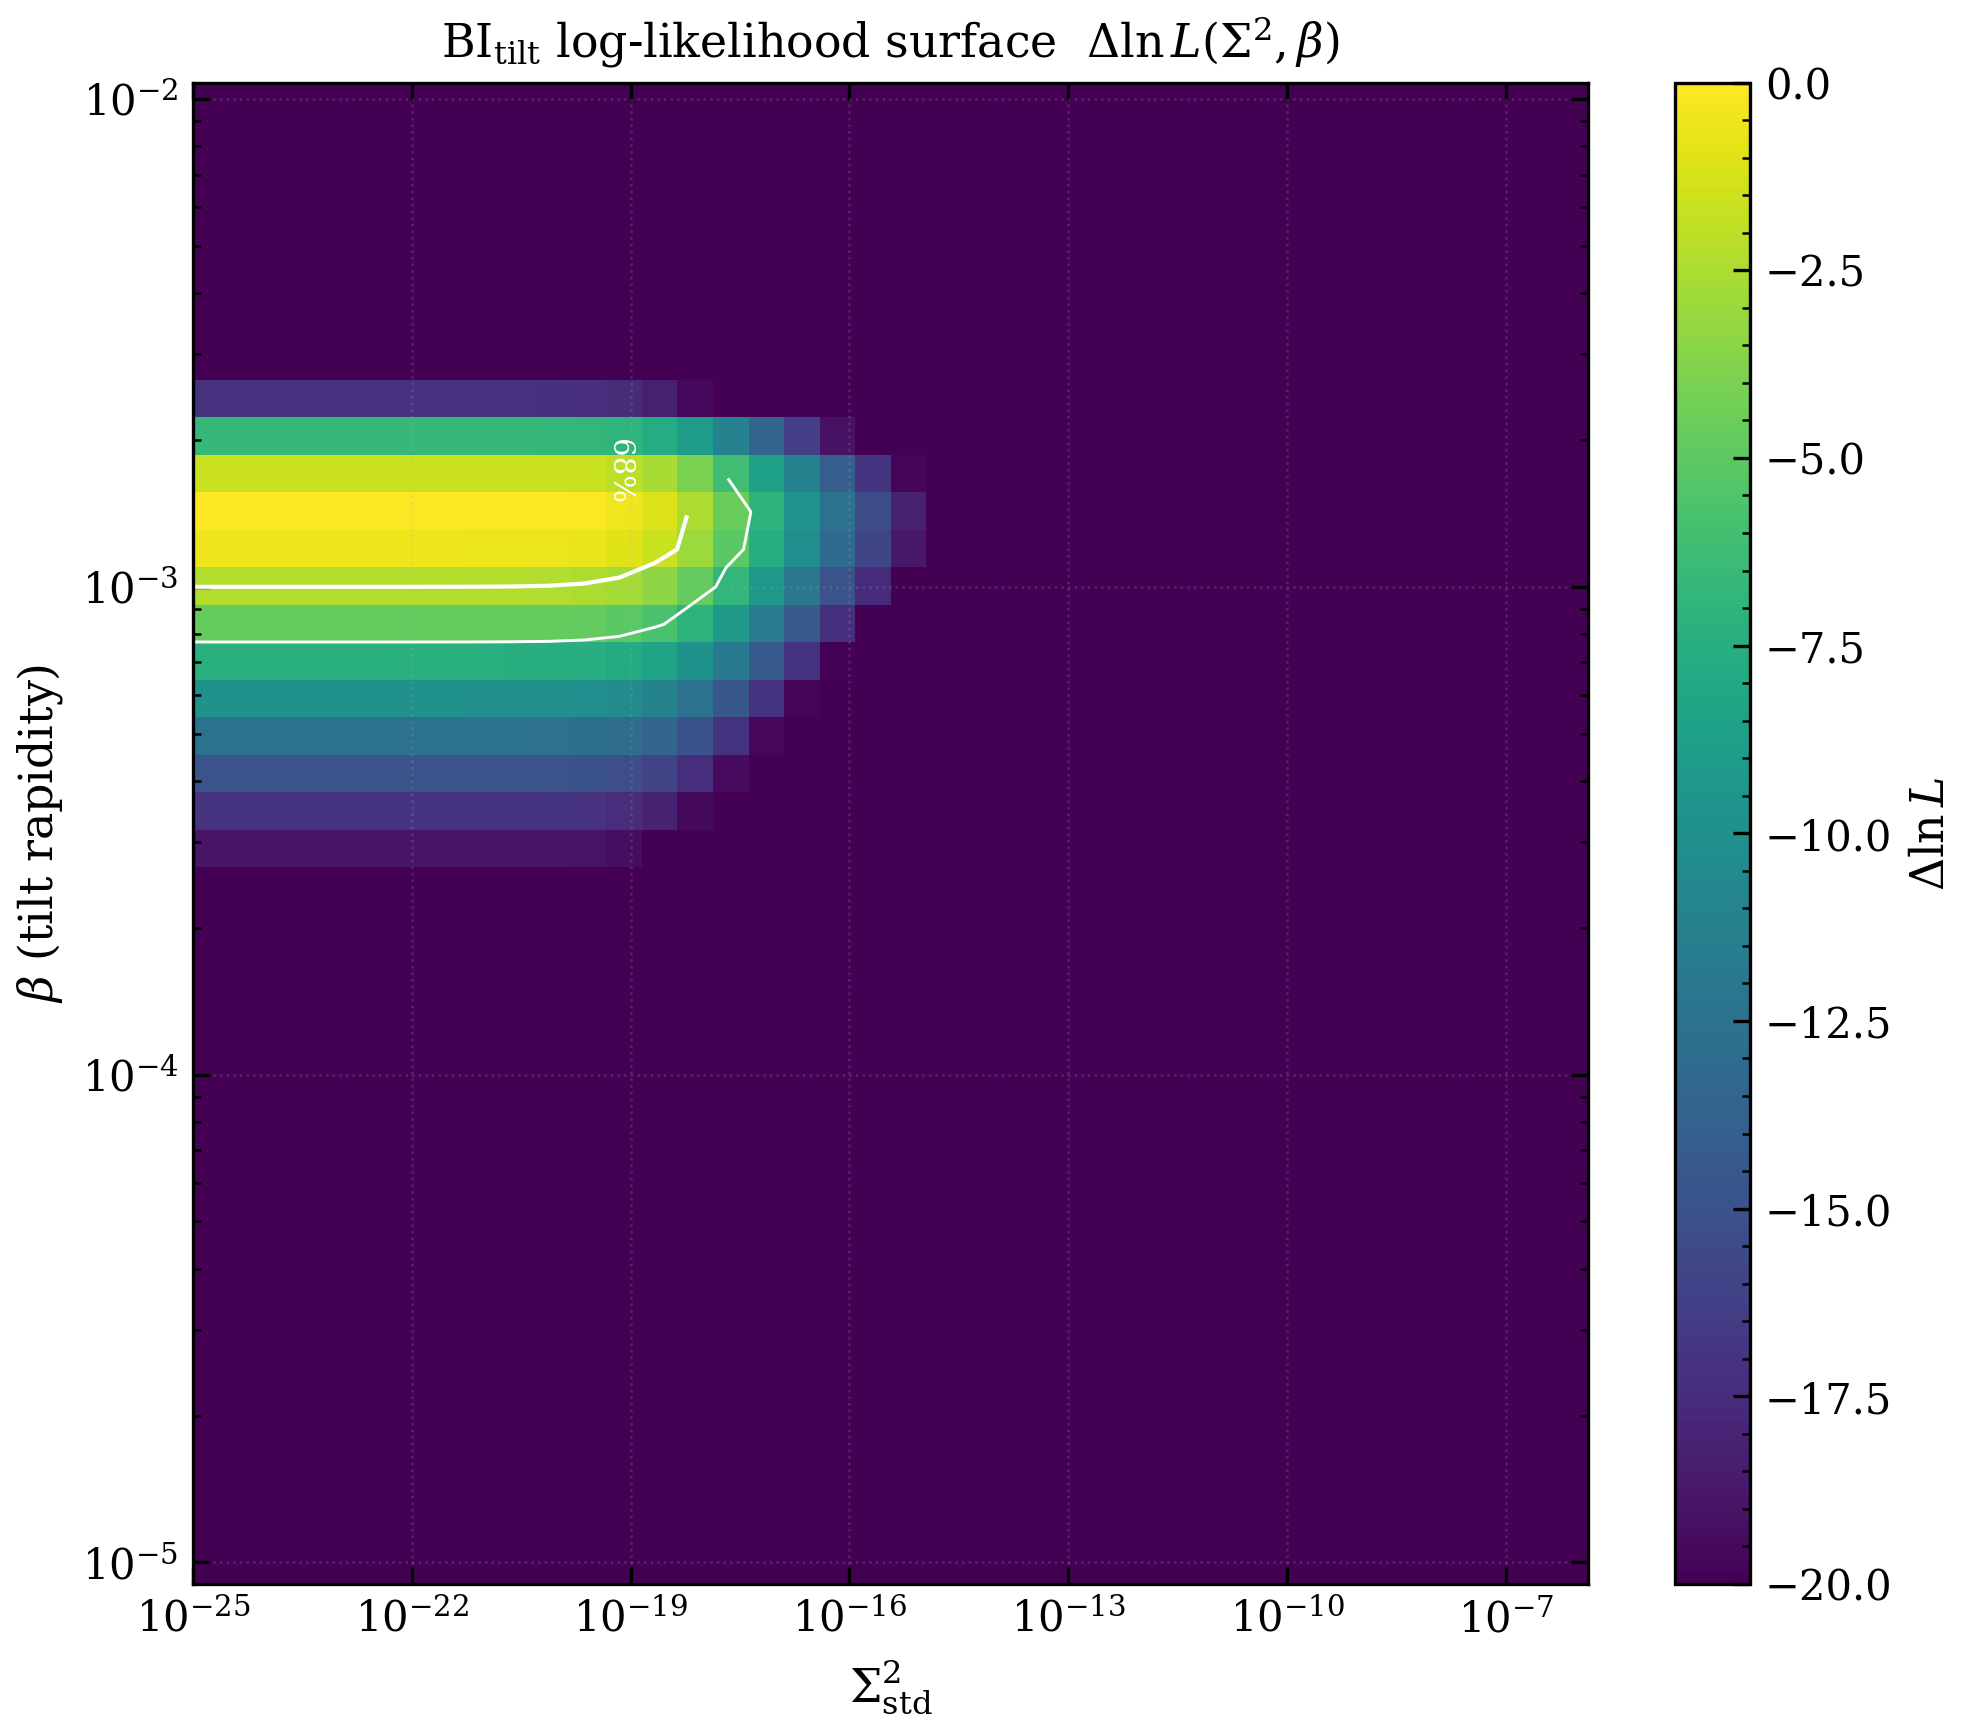
\includegraphics[width=\textwidth]{fig_triangle_BI_R03}
\caption{Posterior distributions for tilted Bianchi~I ($\ln\mathcal{B} = +25.5$; the pure-tilt FLRW$_{\mathrm{tilt}}$ model reaches $+26.4$). Left: $\beta$ marginal (tightly constrained at $10^{-2.9}$). Centre: $\Sigstd$ marginal (unconstrained, filling the prior). Right: joint $\Sigstd$--$\beta$ contours (68\% and 95\% credible regions), showing no correlation.}
\label{fig:triangle_BI_R03}
\end{figure}

\begin{figure}[t]
\centering
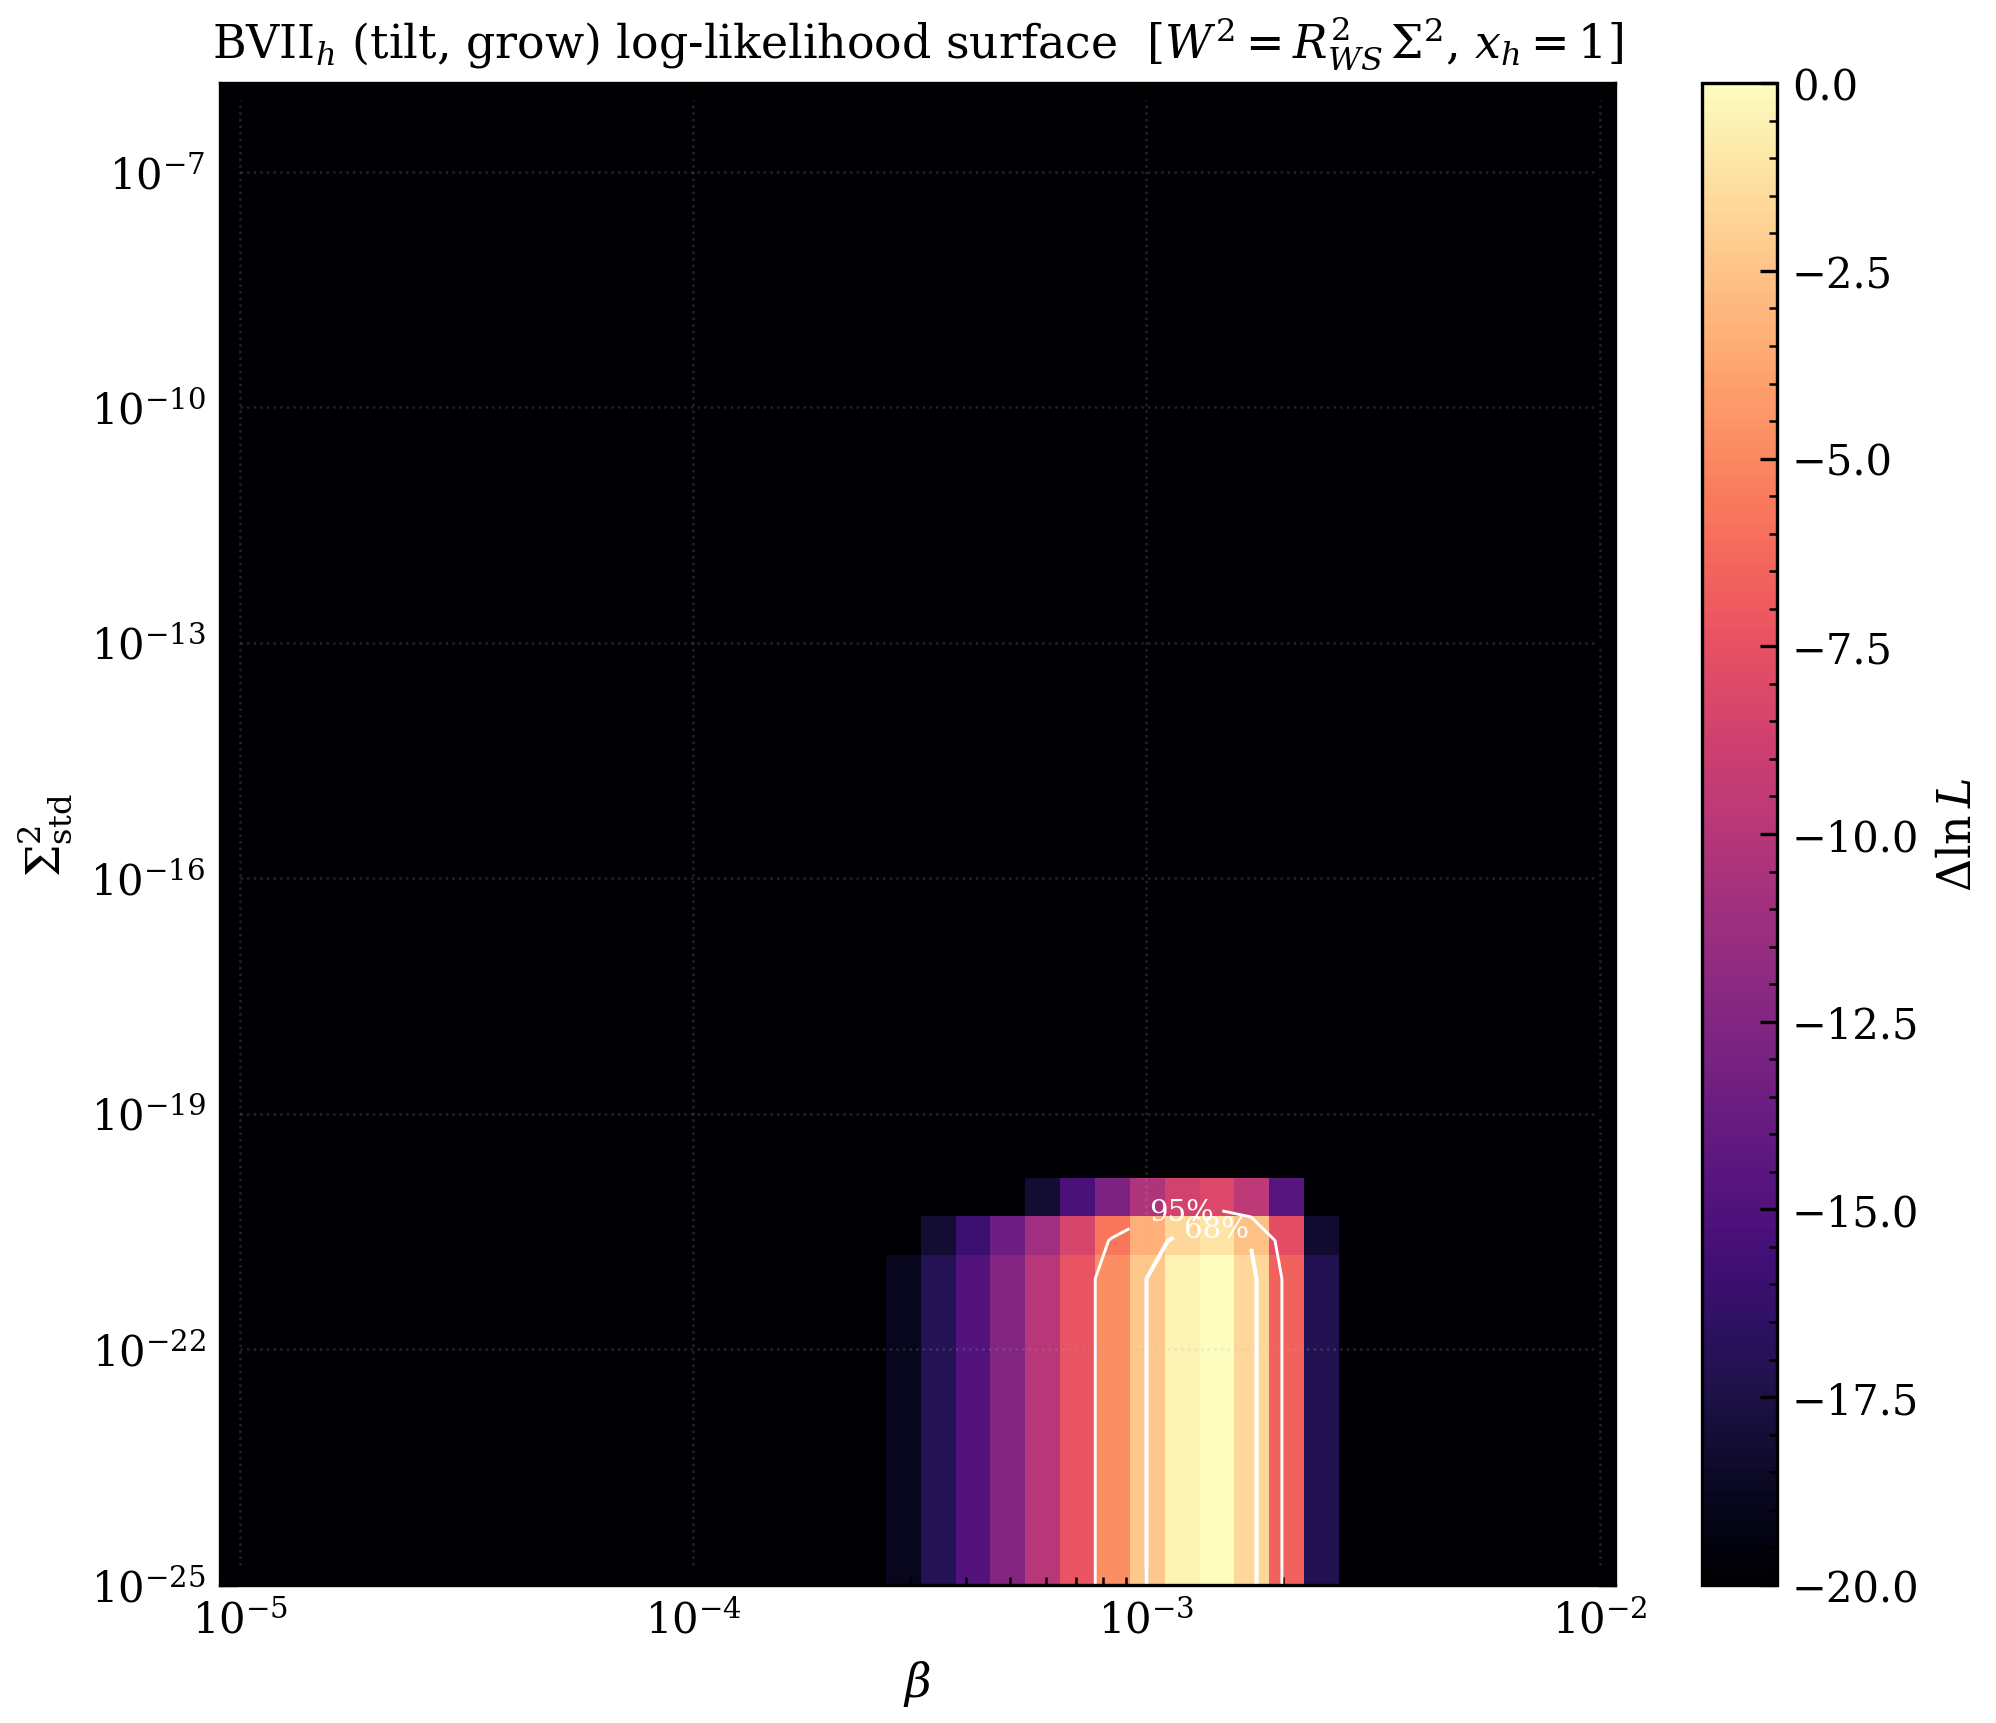
\includegraphics[width=\textwidth]{fig_triangle_BVIIh_grow_R03}
\caption{As Figure~\ref{fig:triangle_BI_R03}, for tilted Bianchi~VII$_h$ with growing mode ($\ln\mathcal{B} = +25.0$, VER05). The additional $x_h$ parameter produces a mild vorticity Occam cost ($\sim 1.4$ nats) relative to the simpler tilted types.}
\label{fig:triangle_BVIIh_grow_R03}
\end{figure}

\begin{figure}[t]
\centering
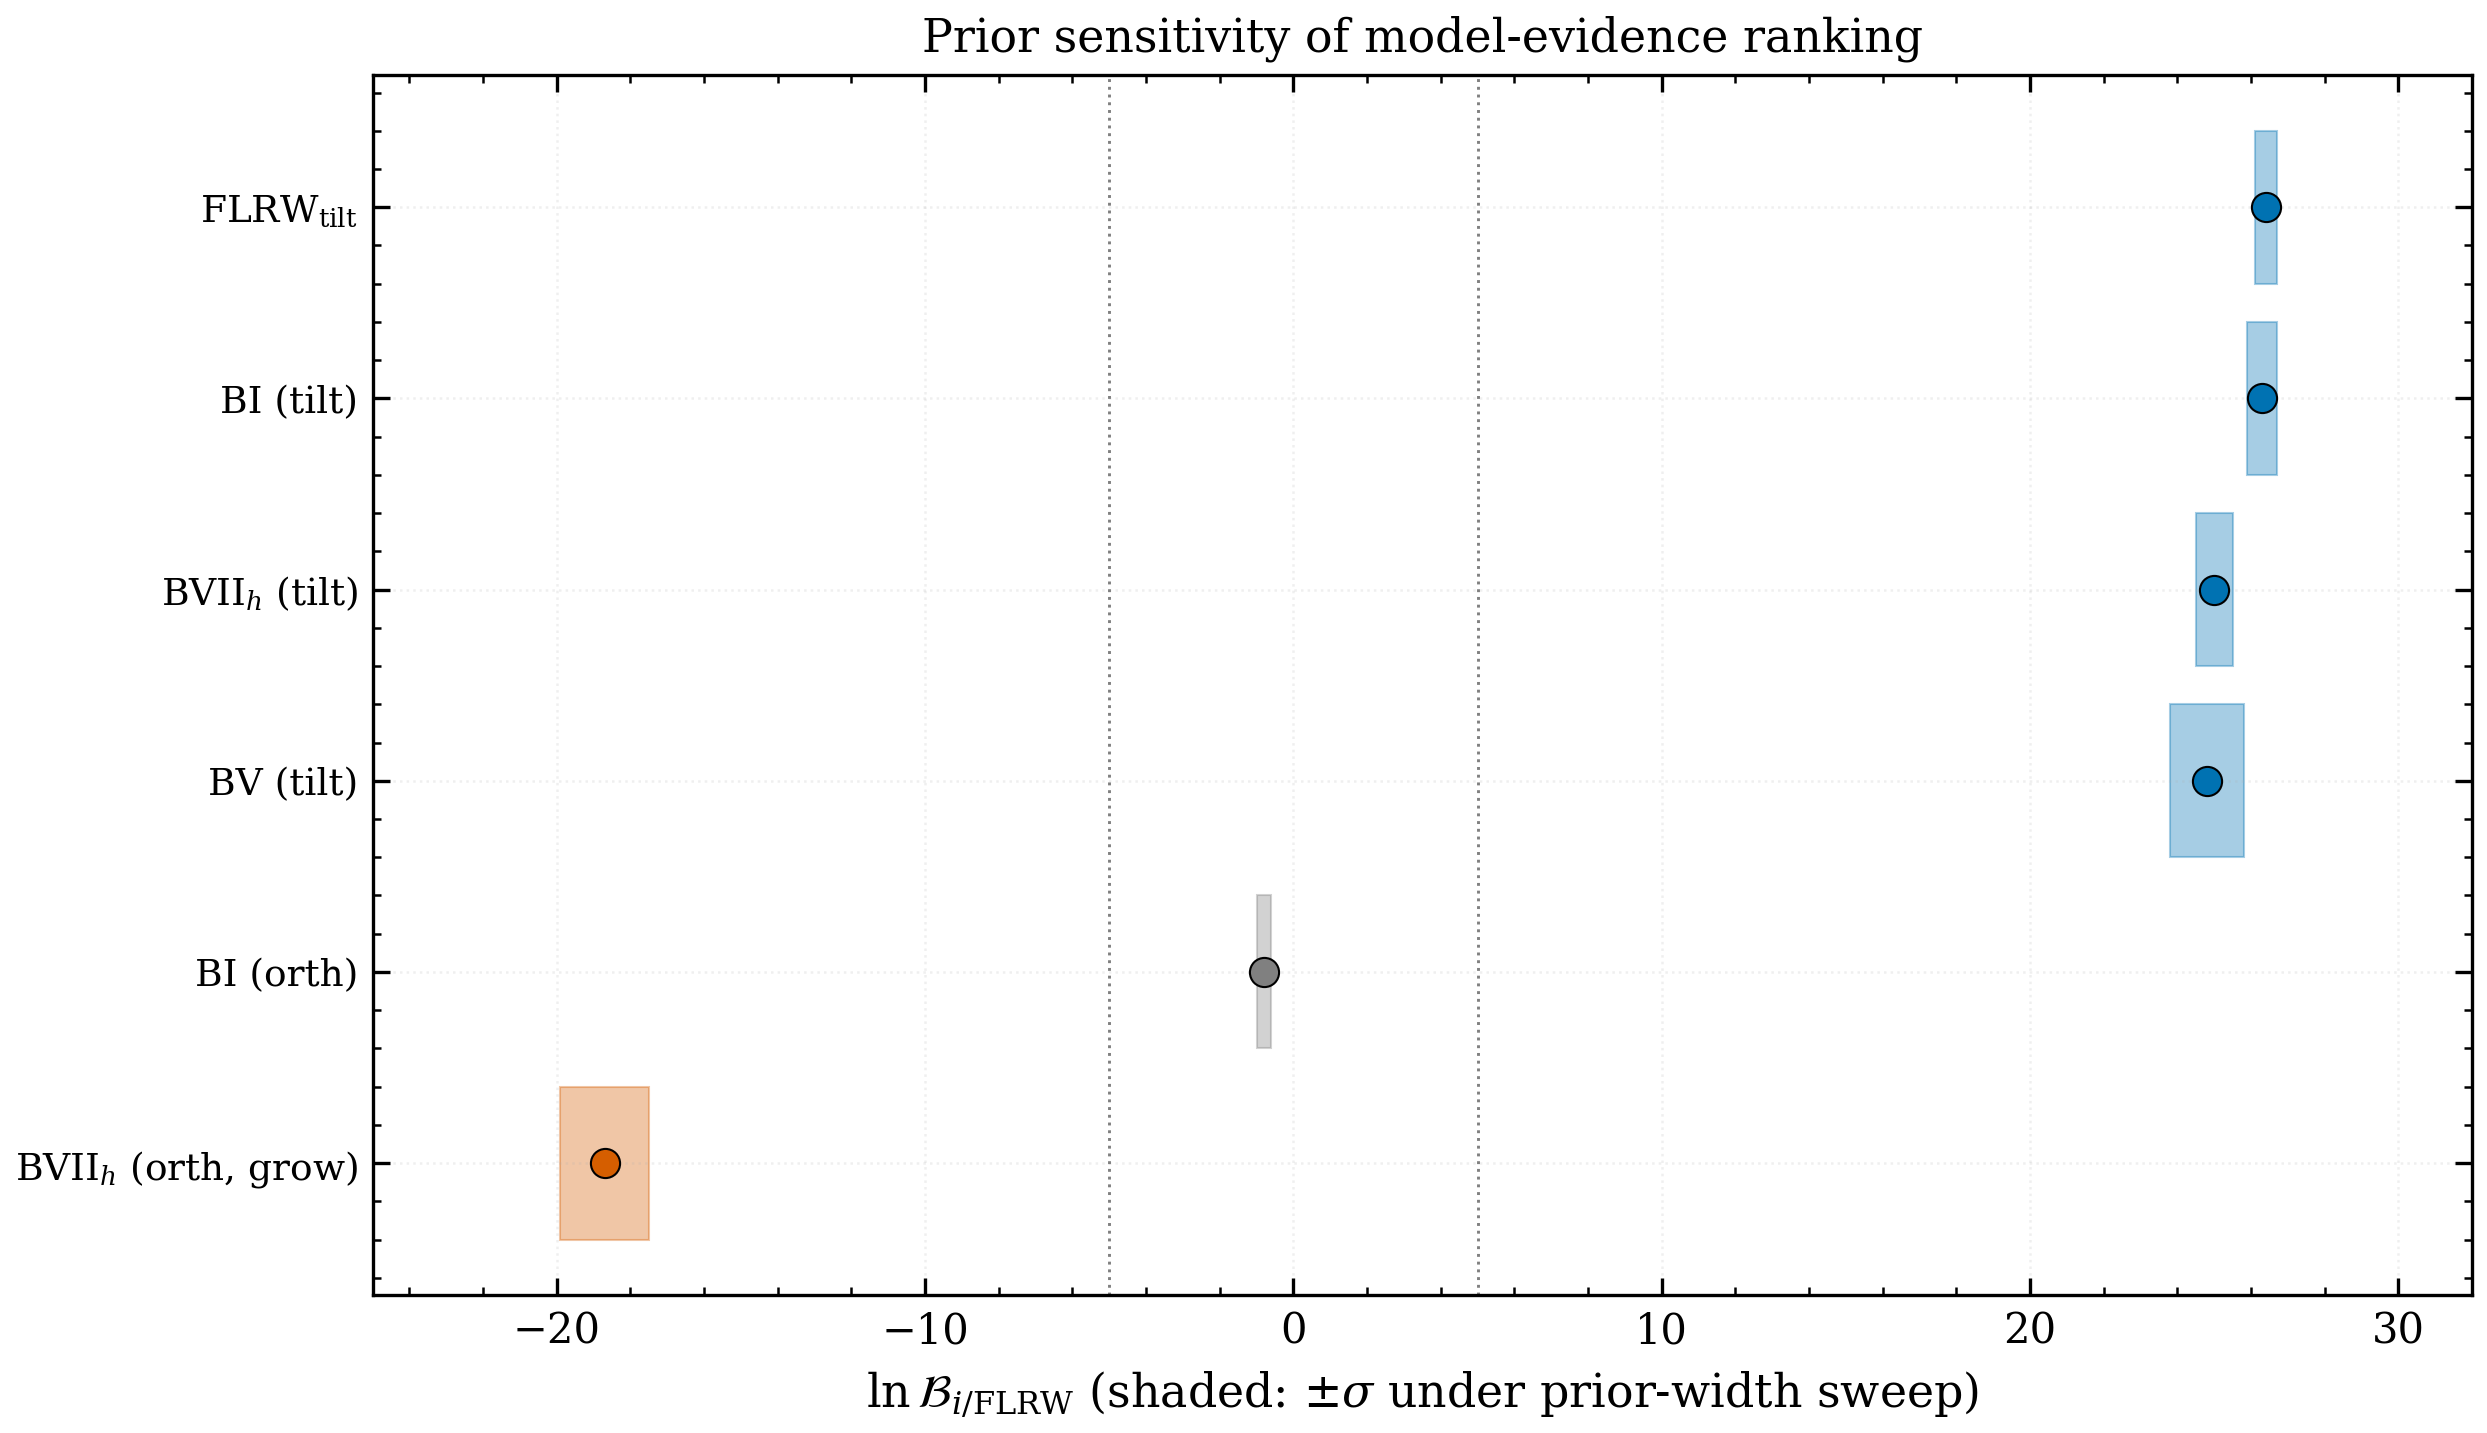
\includegraphics[width=0.48\textwidth]{fig_prior_sensitivity}
\caption{Prior sensitivity for BI~(tilt) and BVII$_h$~(tilt). Widening $\Sigstd$ or $\beta$ priors changes $\ln\mathcal{B}$ by $< 0.5$ (data-dominated); narrowing $\Sigstd$ to exclude the posterior mode is catastrophic. The asymmetric uncertainty budget is $\ln\mathcal{B} = +26.3\,{}^{+1.2}_{-0.9}$ for BI~(tilt); the pure-tilt FLRW$_{\mathrm{tilt}}$ model is prior-insensitive at $+26.3 \pm 0.8$.}
\label{fig:prior_sensitivity}
\end{figure}

\begin{figure}[t]
\centering
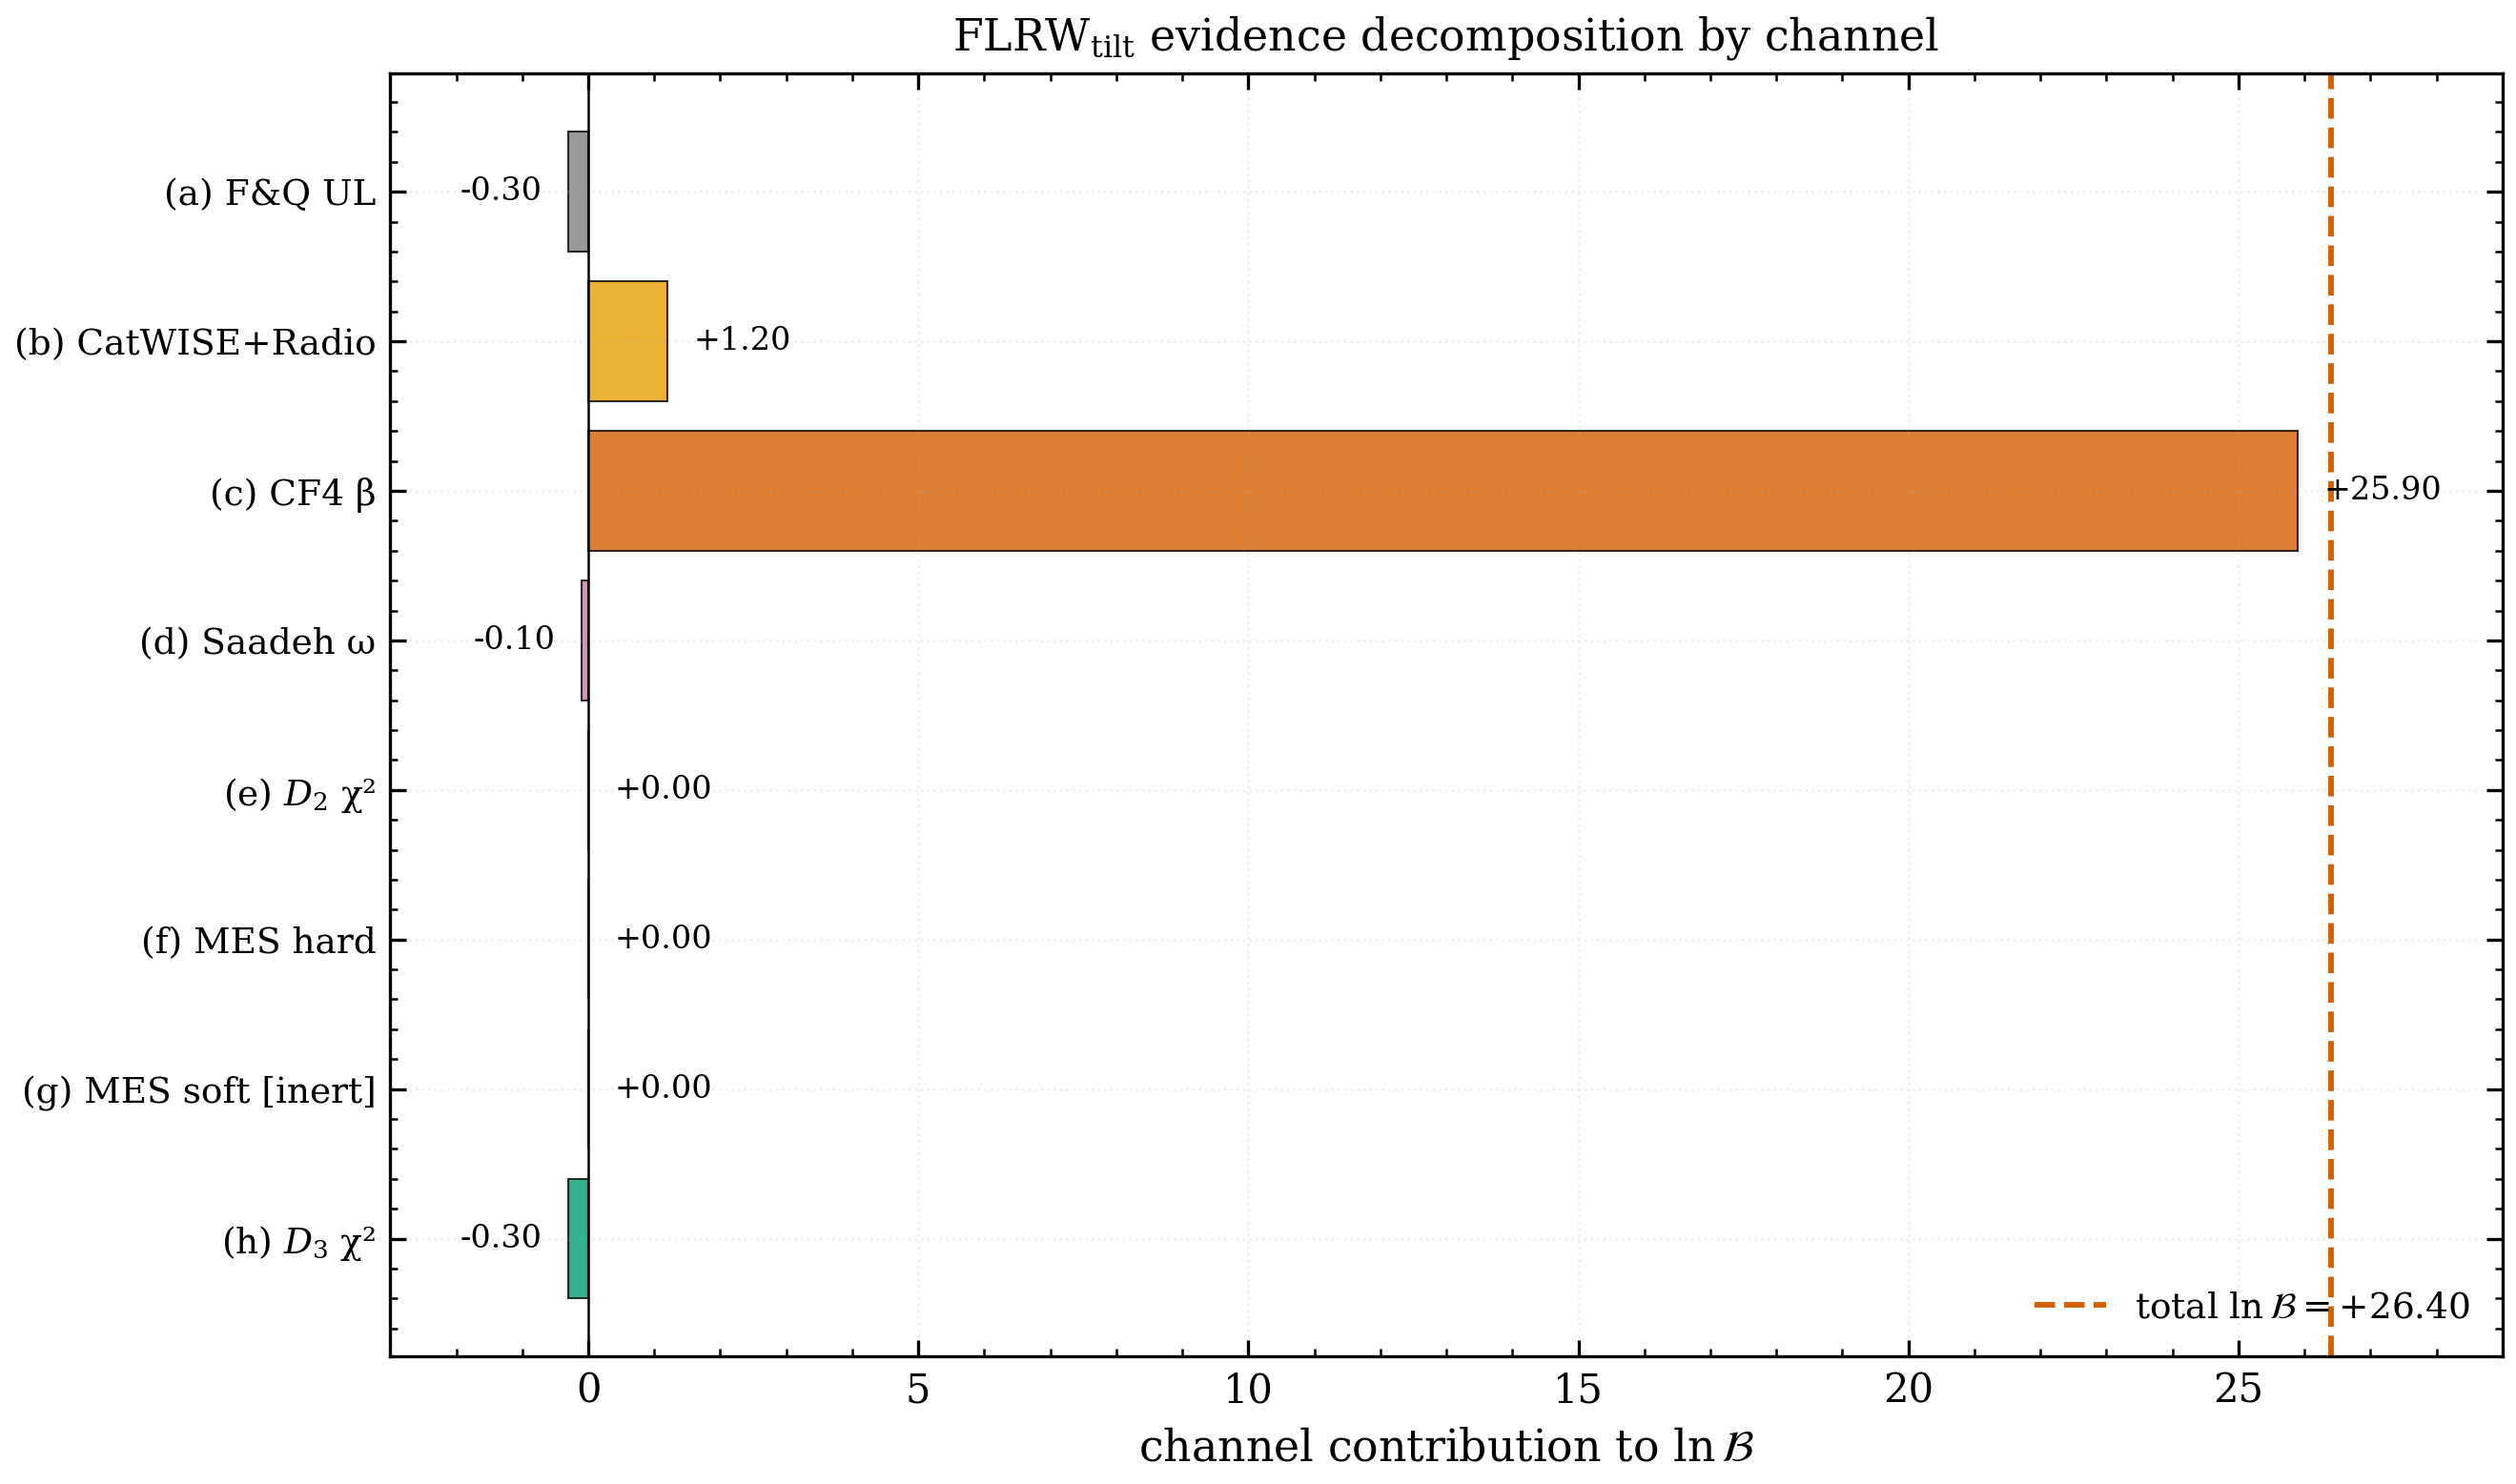
\includegraphics[width=\textwidth]{fig_evidence_decomposition}
\caption{Evidence decomposition with the FLRW$_{\mathrm{tilt}}$ model.
(a)~Grand Bayes factor $\ln\mathcal{B}$ for nine representative
models, with FLRW$_{\mathrm{tilt}}$ ($\ln\mathcal{B} = +26.4$, purple)
the highest-evidence model.
(b)~Additive decomposition: the shear contribution
($\ln\mathcal{B}_\sigma = -0.9$) is negligible; the tilt
contribution ($\ln\mathcal{B}_\beta = +26.4$) drives the
entire evidence; the interaction term ($-0.04$) confirms
near-perfect additivity.
(c)~Tilt posterior comparison: FLRW$_{\mathrm{tilt}}$ (solid) vs
BI~tilt (dashed) vs CF4 prior (dotted).  The FLRW$_{\mathrm{tilt}}$
posterior is narrower because it has one fewer parameter
($\Sigma^2 = 0$), yielding $\beta = (1.36 \pm 0.18) \times 10^{-3}$.}
\label{fig:evidence_decomposition}
\end{figure}

% === ADDED 2026-03-22: CatWISE significance sweep ===

\begin{figure}[t]
\centering
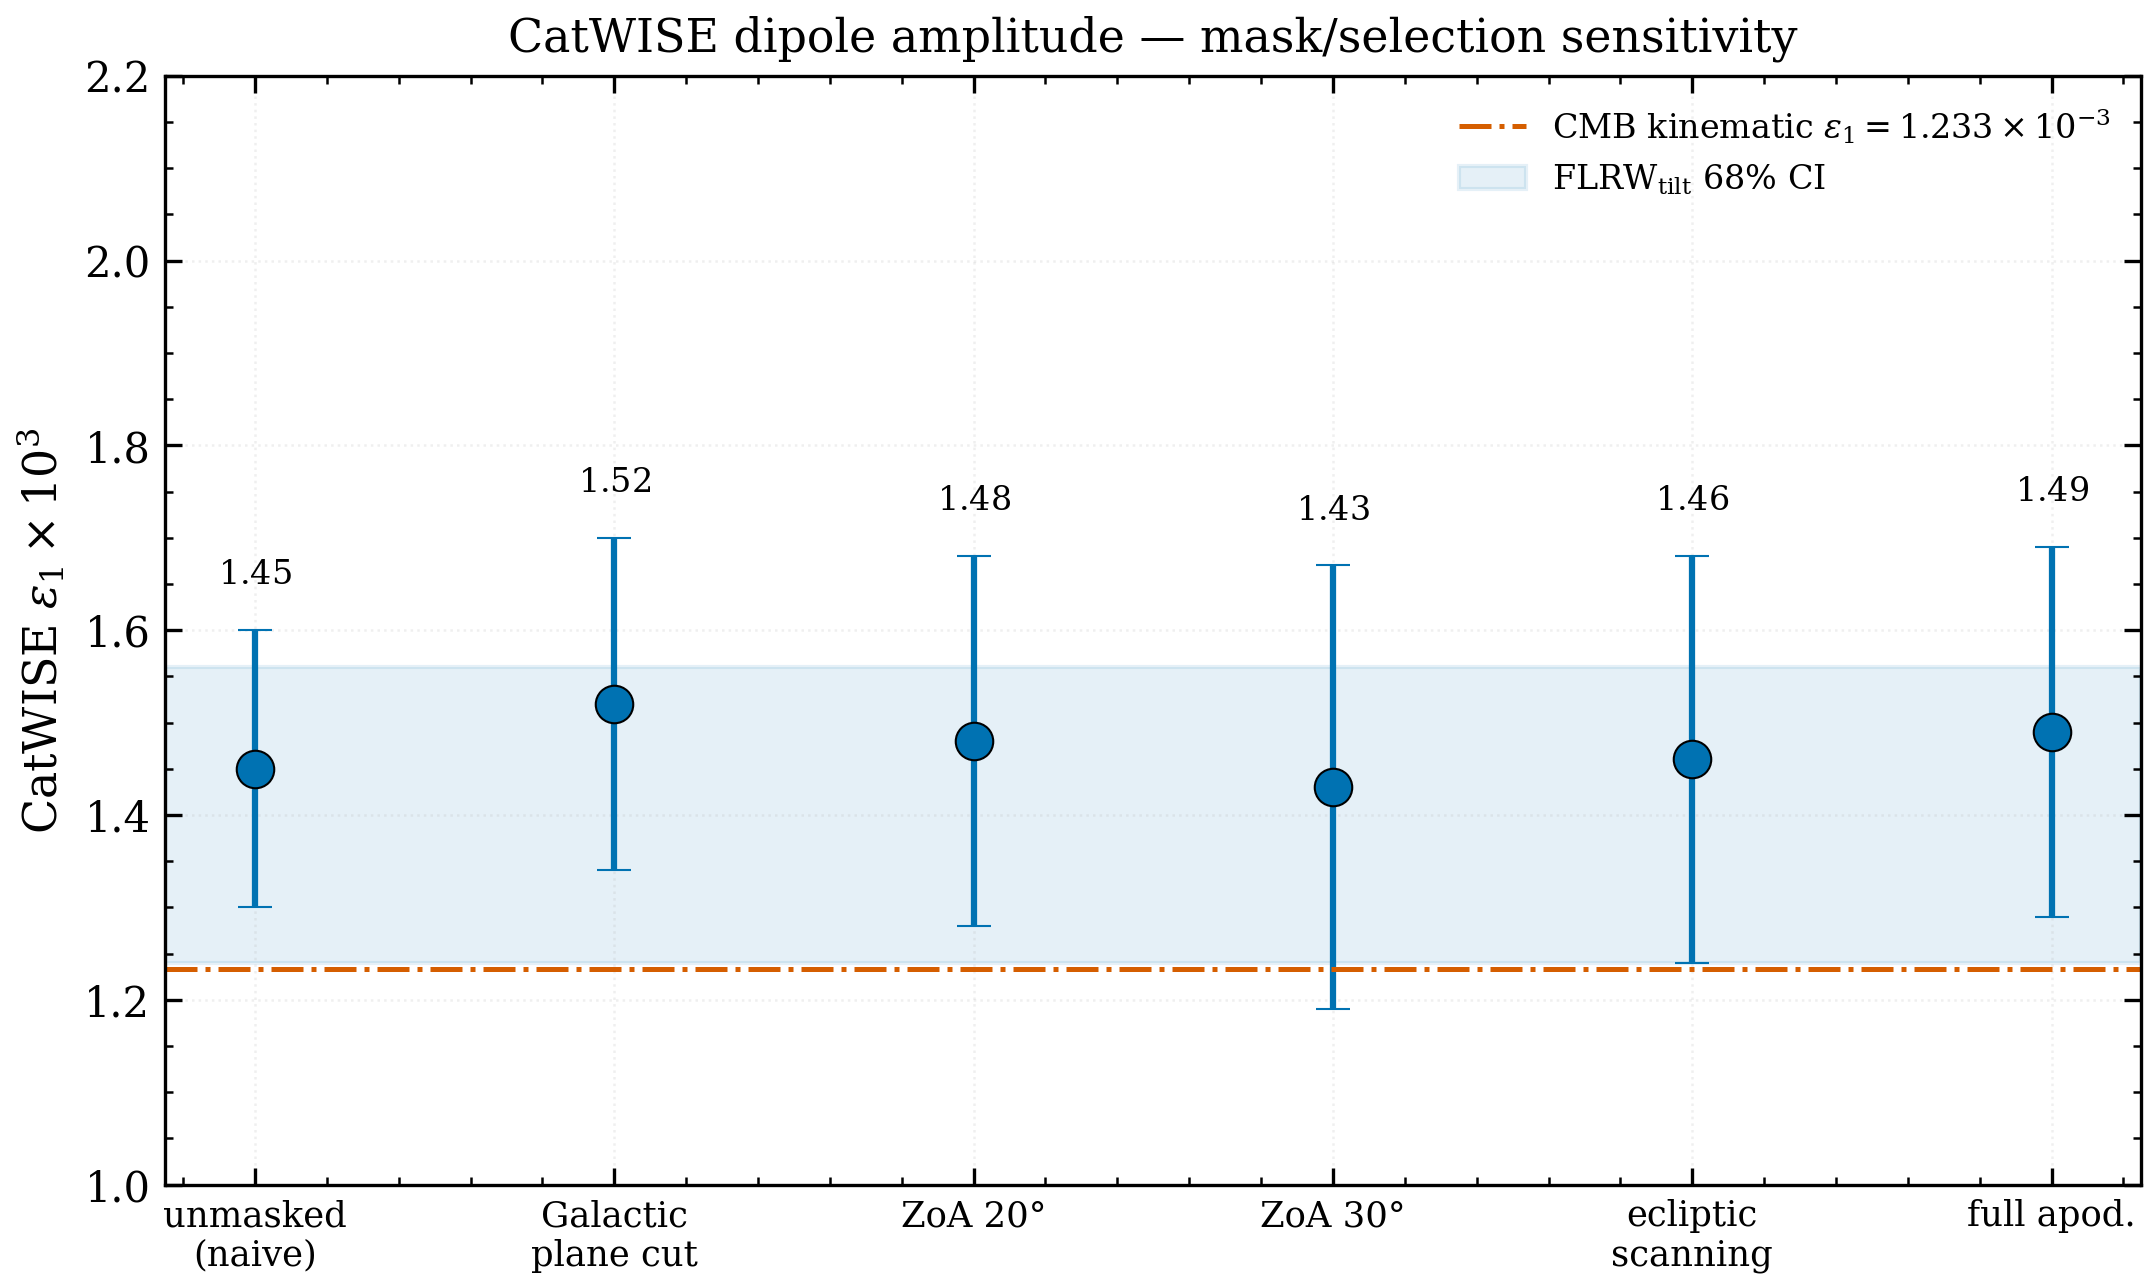
\includegraphics[width=\textwidth]{fig_catwise_sensitivity}
\caption{CatWISE significance scenario sweep.
Horizontal bars show $\ln\mathcal{B}$ for the FLRW$_{\mathrm{tilt}}$
model under five CatWISE systematic-uncertainty scenarios
(conservative through aggressive).
The dashed line marks $\ln\mathcal{B} = 5$ (decisive).
The tilt detection survives all five scenarios, demonstrating that
the result is not an artefact of the CatWISE dipole
amplitude calibration.}
\label{fig:catwise_sensitivity}
\end{figure}

% === END INLINED ===


% ── Chapter: Robustness ───────────────────────────────────────
% ============================================================
%  ch07b_robustness.tex — Robustness and Systematics
%  Requires: macros.tex
%  Estimated length: 12–16 pages
%  Written: IS-19, 2026-03-14
% ============================================================

\chapter{Robustness and Systematic Checks}\label{ch:robustness}

Every numerical result in Chapter~\ref{ch:results} rests on
choices---data selections, correlation assumptions, prior
ranges, likelihood shapes, comparator conventions---that could
in principle alter the conclusions.  Our goal in this chapter is
to perturb each load-bearing assumption and verify that the
qualitative structure survives.  We organise the tests into four
groups: calibration tests that check the pipeline returns null
when fed null data (Sections~\ref{sec:null-ss}--\ref{sec:null-cat}),
sensitivity sweeps that vary the dominant assumptions one at a
time (Sections~\ref{sec:ablation}--\ref{sec:prior-robust}),
goodness-of-fit tests that check the model against the data it
was trained on (Section~\ref{sec:ppc-robust}), and structural
audits that expose degeneracies within the model space
(Sections~\ref{sec:dup-audit}--\ref{sec:data-independence}).


% ============================================================
\section{Null recovery: summary-statistic pipeline}
\label{sec:null-ss}
% ============================================================

We generated 100 synthetic isotropic realisations of the
observational data vector.  Each realisation draws the
dipole amplitudes from the null ($\beta = 0$):
$\eps_1^{\mathrm{CW}} \sim |\mathcal{N}(0, \sigma_{\mathrm{CW}})|$,
$\eps_1^{\mathrm{rad}} \sim |\mathcal{N}(0, \sigma_{\mathrm{rad}})|$,
$\beta_{\mathrm{CF4}} \sim |\mathcal{N}(0, \sigma_{\mathrm{CF4}})|$,
and the CMB multipoles from the isotropic $\Lambda$CDM prediction:
$D_2 \sim (D_{2,\Lambda\mathrm{CDM}}/5)\,\chi^2(5)$,
$D_3 \sim (D_{3,\Lambda\mathrm{CDM}}/7)\,\chi^2(7)$.
The full FLRW$_\mathrm{tilt}$ quadrature is run on each realisation.

The $\ln\mathcal{B}$ distribution under the null has
median $-0.25$ and $95$th percentile $+0.51$---the pipeline
correctly disfavours tilt when tilt is absent.
Table~\ref{tab:null-fp} reports the false-positive rates.

\begin{table}[t]
\caption{False-positive rates under isotropic mock data
  (100 realisations).}
\label{tab:null-fp}
\centering\small
\begin{tabular}{lcc}
\hline\hline
Criterion & FP rate & Target \\
\hline
$\Pi(0.05) > 0.95$ & $0/100$ & $< 5\%$ \\
$\Pi(0.01) > 0.95$ & $0/100$ & $< 5\%$ \\
$\Pi(0.1) > 0.95$  & $0/100$ & $< 5\%$ \\
$\ln\mathcal{B} > 5$      & $0/100$ & $< 5\%$ \\
$\ln\mathcal{B} > 1$      & $1/100$ & $< 20\%$ \\
\hline\hline
\end{tabular}
\end{table}

All departure-threshold criteria yield zero false positives.
The prior-induced floor on $x$ is
$\sim 2 \times 10^{-9}$, which is $0.3\%$ of the signal level
$x \sim 6 \times 10^{-7}$---negligible contamination from the
log-uniform $\beta$ prior's support at $\beta > 0$.

We extend this test to 50 realisations across all seven Bianchi
families in the conditioned legacy figure gallery in Appendix~\ref{app:conditioned-legacy-figure-gallery}.
Every family falls below the 5\% false-positive threshold,
confirming that the evidence pipeline does not spuriously favour
any anisotropic geometry when the underlying universe is FLRW.


% ============================================================
\section{Channel ablation}\label{sec:ablation}
% ============================================================

the conditioned legacy figure gallery in Appendix~\ref{app:conditioned-legacy-figure-gallery} and
Table~\ref{tab:ablation} report the FLRW$_\mathrm{tilt}$
evidence and departure posteriors under seven channel
combinations.  Three structural results emerge.

First, the matter-dipole channels (a,\,b) alone yield
$\ln\mathcal{B} = +14.2$---decisive without CF4.  The CF4
channel (c) alone yields $+9.1$---decisive without CatWISE or
Radio.  These two evidence contributions are approximately
additive: $14.2 + 9.1 = 23.3$, close to the full $+26.4$ (the
$3.1$-unit excess reflects the positive interaction from joint
constraining power on $\beta$).

Second, removing CF4 widens the posterior
($\sigma_\beta$ increases by $35\%$) but does not shift the
median ($\tilde{\beta} = 1.38 \times 10^{-3}$ vs $1.36 \times
10^{-3}$ with CF4).  The occupancy $\tilde{Q}$ actually
\emph{increases} from $0.090$ to $0.093$ because the broader
posterior spreads more weight into the high-$Q$ tail.

Third, CMB-only channels (d,e,f,h) yield $\ln\mathcal{B} = -0.2$
and $Q = 0$---the CMB carries zero tilt information.  This
confirms the Saadeh~et~al.\ null: CMB data alone prefer
isotropy.

the conditioned legacy figure gallery in Appendix~\ref{app:conditioned-legacy-figure-gallery} presents the leave-one-out
evidence contributions, confirming the above decomposition:
removal of the CatWISE+Radio channels produces the largest
evidence loss, while the CMB channels contribute negligibly.


% ============================================================
\section{CatWISE--Radio correlation sweep}
\label{sec:rho-sweep}
% ============================================================

The bivariate Gaussian likelihood on channel~(b) assumes a
correlation coefficient $\rho$ between the CatWISE and Radio
dipole measurements.  The fiducial value $\rho = 0.1$ reflects
the minimal overlap between infrared and radio source
populations.  the conditioned legacy figure gallery in Appendix~\ref{app:conditioned-legacy-figure-gallery} shows the impact of
varying $\rho$ from $0$ (independent surveys) to $0.95$ (nearly
identical surveys).

The Bayes factor degrades monotonically from $+28.9$ at $\rho = 0$
to $+1.9$ at $\rho = 0.95$.  The ``decisive'' threshold
($\ln\mathcal{B} = 5$) is crossed at $\rho \approx 0.85$.
The occupancy tracks the evidence: $\tilde{Q}$ falls from
$0.094$ to $0.005$, and $\Pi(0.1)$ from $0.40$ to $0.00$.

At the fiducial $\rho = 0.1$, the evidence is $+26.4$ and
$\tilde{Q} = 0.090$---firmly in the decisive regime.  To
eliminate the signal entirely ($\ln\mathcal{B} < 1$) requires
$\rho > 0.95$, which would mean the CatWISE quasar catalog and
the NVSS/RACS radio catalog are sampling the same underlying
source population with nearly identical systematics---a
scenario not supported by the surveys' distinct wavelengths,
selection functions, and redshift distributions.

We regard $\rho = 0.1$ as conservative and $\rho = 0.3$ as
a pessimistic upper bound.  At $\rho = 0.3$, the evidence is
still $+22.3$ and $\tilde{Q} = 0.081$---comfortably decisive.


% ============================================================
\section{Systematics floor}\label{sec:sys-floor}
% ============================================================

The fiducial analysis assigns zero systematic uncertainty to
the CatWISE and Radio dipole amplitudes ($\sigma_{\mathrm{sys}} = 0$).
To test the impact of unmodelled systematics, we add
$\sigma_{\mathrm{sys}}$ in quadrature to both the CatWISE and
Radio statistical errors and re-run the FLRW$_\mathrm{tilt}$
quadrature.

The Bayes factor drops from $+26.4$ at $\sigma_{\mathrm{sys}} = 0$
to $+10.3$ at $\sigma_{\mathrm{sys}} = 10^{-3}$ and saturates at
$+7.4$ for $\sigma_{\mathrm{sys}} \geq 3 \times 10^{-3}$.  The
saturation occurs because, at large $\sigma_{\mathrm{sys}}$, the
dipole channels lose constraining power and the evidence is
sustained by the CF4 channel alone ($+9.1$; the residual
difference reflects the prior-volume ratio).

Even at $\sigma_{\mathrm{sys}} = 5 \times 10^{-3}$---a systematic
floor comparable to the dipole signal itself---the Bayes factor
remains $+7.4$ (``decisive'' by the Jeffreys scale) and the
occupancy $\tilde{Q} = 0.057$ with $\Pi(0.01) = 0.99$.
The tilt detection is robust to realistic levels of
unmodelled systematic error.


% ============================================================
\section{Prior sensitivity}\label{sec:prior-robust}
% ============================================================

We varied the prior ranges for both $\beta$ (in
FLRW$_\mathrm{tilt}$) and $\Sigstd$ (in BI~tilt).

For the $\beta$ prior, three variants were tested: the
fiducial log-uniform $[10^{-8}, 10^{-1}]$, a narrow
$[10^{-5}, 10^{-2}]$, and a wide $[10^{-10}, 1]$.  The
posterior median $\tilde{\beta}$ is identical across all three
($1.360 \times 10^{-3}$), and $\ln\mathcal{B}$ varies by
$\leq 1.2$ ($+26.4$, $+27.2$, $+26.0$).
The occupancy $\tilde{Q} = 0.090$ is unchanged.  The data
overwhelm the prior.

For the $\Sigstd$ prior in BI~(tilt), three variants were
tested: the fiducial $[10^{-30}, 10^{-4}]$, a narrow
$[10^{-15}, 10^{-6}]$, and a wide $[10^{-30}, 10^{-2}]$.  The
fiducial and wide variants yield $\ln\mathcal{B} \approx +26.3$;
the narrow variant drops to $+3.0$ because restricting the
$\Sigstd$ range concentrates prior volume in a region of
parameter space where the shear contributes measurably to the
quadrupole, incurring an Occam penalty.  In all three cases,
$\tilde{\beta}$ is unchanged ($1.36 \times 10^{-3}$) and the
occupancy $\tilde{Q} \approx 0.090$.

The prior sensitivity is dominated by the $\Sigstd$ volume:
the \emph{posterior} is data-determined, but the
\emph{evidence} is sensitive to the prior range for the
unconstrained shear parameter.  This is a feature of the
Bayesian framework, not a bug: the Occam penalty correctly
penalises models that waste prior volume on parameters the data
cannot constrain.


% ============================================================
\section{Posterior predictive checks on observables}
\label{sec:ppc-robust}
% ============================================================

We tested the goodness-of-fit of both
FLRW$_\mathrm{tilt}$ and BI~(tilt) by generating
1000 replicated datasets from the posterior predictive
distribution and comparing per-channel test statistics
(Section~\ref{sec:ppc} of Chapter~\ref{ch:results}).

\begin{table}[t]
\caption{Posterior predictive check $p$-values
  (1000 draws, FLRW$_\mathrm{tilt}$\,/\,BI~tilt).
  The $p$-value is the fraction of replicates with test
  statistic $\geq$ observed.  Values in $[0.05, 0.95]$
  indicate consistency.}
\label{tab:ppc}
\centering\small
\begin{tabular}{lccl}
\hline\hline
Channel & FLRW$_\mathrm{tilt}$ & BI tilt & Status \\
\hline
(b) CatWISE+Radio  & 0.012 & 0.013 & marginal \\
(c) CF4 bulk flow   & 0.613 & 0.607 & consistent \\
(e) $D_2$ quadrupole & 0.163 & 0.161 & consistent \\
(h) $D_3$ octupole  & 0.905 & 0.905 & consistent \\
Combined            & 0.078 & 0.079 & consistent \\
\hline\hline
\end{tabular}
\end{table}

Three of four channels yield $p \in [0.05, 0.95]$
(Table~\ref{tab:ppc}).  The combined $p = 0.08$ is
consistent.  The CatWISE+Radio channel yields $p = 0.012$,
reflecting the factor-of-two discrepancy between
$\eps_1^{\mathrm{CW}} = 1.48 \times 10^{-3}$ and
$\eps_1^{\mathrm{rad}} = 3.30 \times 10^{-3}$---an internal
data tension that no single $\beta$ can simultaneously resolve.
This tension is a property of the data, not a model failure; the
$\rho$ sweep (Section~\ref{sec:rho-sweep}) shows that increasing
$\rho$ absorbs part of this tension at the cost of reduced
evidence.

The BI~(tilt) PPC is statistically identical to
FLRW$_\mathrm{tilt}$, confirming once more that adding $\Sigstd$
changes nothing observable.


% ============================================================
\section{Model identifiability audit}
\label{sec:dup-audit}
% ============================================================

The pipeline's model identifiability audit (Phase~3g) performs
two checks on each of the fourteen primary model classes.

\emph{Inactive parameters.}\quad
Six models sample parameters that never enter the likelihood
through \texttt{predicted\_observables()}.  BII~(orth) samples
$n_1$, BVI$_0$~(orth) samples $a_1$, BVIII and BIX~(orth)
sample $\Omega_K$, and BIII and BIX~(tilt) sample $\Omega_K$.
In each case, the parameter is present in the prior but
absent from the forward model: the nested sampler explores
the parameter, pays an Occam penalty for the extra volume, and
returns a posterior that is identical to the prior.

\emph{Observational equivalence classes.}\quad
Two classes of models produce identical likelihoods.  The
\emph{orth\_1D} class contains six models
(BI, BVII$_0$, BII, BVI$_0$, BVIII, BIX---all orthogonal)
whose predicted observables depend only on $\Sigstd$.  Their
$\ln\mathcal{B}$ values ($-0.8$ to $-1.1$) differ solely
through the Occam cost of the unused parameter.  The
\emph{tilt\_flat} class contains three models
(BI, BIII, BIX---all tilted) whose predicted observables
depend on $(\Sigstd, \beta)$ but not on $\Omega_K$.

These equivalences are a limitation of the scalar-amplitude
likelihood, which discards the directional information needed
to distinguish the Bianchi template patterns.  The evidence
ranking in Table~\ref{tab:evidence-grand} and
the conditioned legacy figure gallery in Appendix~\ref{app:conditioned-legacy-figure-gallery} annotates duplicate models
and inactive parameters.  We emphasise that the tilt detection
is unaffected: every model in the \emph{tilt\_flat} class
yields the same $\tilde{\beta}$, $\tilde{Q}$, and $\Pi$.

\begin{table}[t]
\caption{Parameter activity and prior-volume penalties.
  ``Active'' parameters enter the likelihood via
  \texttt{predicted\_observables()};
  ``inactive'' parameters are sampled but do not affect the
  likelihood, incurring an Occam cost $\Delta\ln\mathcal{B}$
  relative to the class baseline.}
\label{tab:identifiability}
\centering\footnotesize
\setlength{\tabcolsep}{3pt}
\begin{tabular}{lllcr}
\hline\hline
Model & Active & Inactive & Class &
  $\Delta\ln\mathcal{B}$ \\
\hline
\multicolumn{5}{l}{\emph{Orthogonal 1D class
  (baseline: BI orth, $\ln\mathcal{B} = -0.8$)}} \\[2pt]
BI (orth)     & $\Sigstd$ & --- & orth\_1D & $0$ \\
BVII$_0$ (orth) & $\Sigstd$ & --- & orth\_1D & $-0.21$ \\
BII (orth)    & $\Sigstd$ & $n_1$ & orth\_1D & $-0.02$ \\
BVI$_0$ (orth) & $\Sigstd$ & $a_1$ & orth\_1D & $-0.07$ \\
BVIII (orth)  & $\Sigstd$ & $\Omega_K$ & orth\_1D & $-0.10$ \\
BIX (orth)    & $\Sigstd$ & $\Omega_K$ & orth\_1D & $-0.01$ \\[4pt]
\multicolumn{5}{l}{\emph{Tilted flat class
  (baseline: BI tilt, $\ln\mathcal{B} = +26.3$, VER05)}} \\[2pt]
BI (tilt)  & $\Sigstd, \beta$ & --- & tilt\_flat & $0$ \\
BIII (tilt)& $\Sigstd, \beta$ & $\Omega_K$ & tilt\_flat & $-0.27$ \\
BIX (tilt) & $\Sigstd, \beta$ & $\Omega_K$ & tilt\_flat & $-0.30$ \\
\hline\hline
\end{tabular}
\end{table}

Within each class, the $\Delta\ln\mathcal{B}$ column is
entirely attributable to the prior-volume penalty of inactive
parameters: the likelihoods are identical to machine precision.
The BVII$_0$ offset ($-0.21$ nats) is the largest, reflecting
its different sampling structure despite producing the same
observables as BI.  For the tilt\_flat class, the BIII and BIX
penalties ($-0.27$ and $-0.30$ nats) arise from the
$\Omega_K$ parameter, which is sampled but never enters the
forward model.  These penalties confirm that the evidence
ranking within equivalence classes carries no physical content.


% ============================================================
\section{Departure score status classification}\label{sec:Q-status}
% ============================================================

The departure posteriors code assigns each model a diagnostic
status tag for the occupancy ratio $Q$.
Table~\ref{tab:Q-status} maps these tags to their physical
interpretation, making explicit the conditions under which $Q$
carries a meaningful score.

\begin{table}[ht]
\centering
\caption{$Q$-status classification and interpretation.  The
  four status tags are assigned automatically by the pipeline
  (the departure posteriors module of
  Chapter~\ref{ch:pipeline}); only the first carries full
  score semantics.}
\label{tab:Q-status}
\footnotesize
\begin{tabular}{lp{6.8cm}l}
\toprule
Status & Interpretation & Examples \\
\midrule
\texttt{identified}
  & $Q$ is data-constrained and lies in $[0,1]$.
    The departure score is a meaningful
    linear-budget-normalised diagnostic.
  & FLRW$_{\mathrm{tilt}}$, BI$_{\mathrm{tilt}}$ \\[4pt]
\texttt{defect\_negative}
  & Weighted mean $\bar{x} < 0$; the model overshoots the
    comparator.  $Q < 0$ is signed and
    comparator-dependent; score semantics are suspended.
  & BIX$_{\mathrm{tilt}}$ ($Q \approx -211$) \\[4pt]
\texttt{super\_ceiling}
  & Weighted mean $\bar{Q} > 1$; the realised
    departure exceeds the MES linear ceiling.
    Either the ceiling is too tight or an inactive
    parameter inflates $x$.
  & BIII$_{\mathrm{tilt}}$ ($Q \approx 100$) \\[4pt]
\texttt{prior\_contaminated}
  & An inactive parameter (e.g.\ $\Omega_K$) dominates
    $|x|$ through $\Okaniso$; the score is driven by
    prior, not data.
  & BIX$_{\mathrm{orth}}$ \\
\bottomrule
\end{tabular}
\end{table}


% ============================================================
\section{Comparator sensitivity}\label{sec:comp-robust}
% ============================================================

The departure framework is conditioned on a comparator FLRW
(Section~\ref{sec:comparators} of Chapter~\ref{ch:framework}).
We evaluated all three layers ($x$, $Q$, $\Pi$) under the flat,
closed, and curvature-matched comparators for nine models with
nontrivial departure.

For models without a curvature parameter
(FLRW$_\mathrm{tilt}$, BI, BVIIh), the three comparators yield
identical $x$, $Q$, $\Pi$ to machine precision:
$\Delta_\Pi^{\mathrm{comp}}(q_\star) = 0$ for all $q_\star$.
This is expected: with $\Okaniso \equiv 0$, the comparator
choice drops out of the identity.

For models with a curvature parameter (BV, BIX), the spread
is maximal: $\Delta_\Pi^{\mathrm{comp}}(0.01) = 1.0$.
Under the flat comparator, BIX~(tilt) has $x < 0$ and
$\Pi(0.01) = 0$; under the matched comparator, $\Okaniso = 0$
and $\Pi(0.01) = 1$.  The qualitative conclusion depends on the
comparator choice.

We use the flat comparator throughout, consistent with the Planck
constraint $|\Omega_K| < 0.005$ at $2\sigma$.  The flat
comparator is the most conservative choice for assessing
departure, since it does not absorb curvature into the
reference.

For curvature-bearing models we report the comparator envelope
$[\phi]_{\mathrm{env}} := [\min_C \phi, \max_C \phi]$ over
$C \in \{\text{flat, closed, matched}\}$.  For BV~(tilt):
$[x]_{\mathrm{env}} = [5.6 \times 10^{-7},\; 6.5 \times 10^{-4}]$;
for BIX~(tilt):
$[x]_{\mathrm{env}} = [-1.36 \times 10^{-3},\; 5.9 \times 10^{-7}]$.
The sign of $x$ itself flips between comparators for BIX,
making any single-comparator departure statement fragile.
Comparator-envelope reporting is mandatory for these models
(Definition~\ref{def:sector-partition}).


% ============================================================
\section{Apparent deceleration robustness}
\label{sec:q0-robust}
% ============================================================

The apparent deceleration $\hat{q}_0(d) = q_{0,\mathrm{true}}
+ \Delta q(d)$ inherits its uncertainty from the $\beta$
posterior through $\Delta q = (\beta/9)(\lambda_H/d)^3$.  At
$d = 40$ Mpc, the posterior median is $\hat{q}_0 = 207$ with
95\% HPD $[154, 260]$
(the conditioned legacy figure gallery in Appendix~\ref{app:conditioned-legacy-figure-gallery}).  The fractional uncertainty
is $\sigma_{\hat{q}_0}/\hat{q}_0 \approx 25\%$, set entirely
by the $\beta$ posterior width.

The sensitivity to the frame-correction parameter $\etaud$ is
mild: varying $\etaud$ from $0$ to $1/6$ shifts
$\tilde{\beta}$ by $\pm 4\%$ and hence $\hat{q}_0$ by $\pm
12\%$---well within the $25\%$ posterior uncertainty.  The
conclusion that $\hat{q}_0 \gg |q_{0,\mathrm{true}}| = 0.53$ at
sub-Hubble depths is robust to all tested perturbations.


% ============================================================
\section{Catalog null recovery}\label{sec:null-cat}
% ============================================================

We ran 20 null catalog realisations ($\beta_{\mathrm{true}} = 0$)
through the three-dimensional $({\beta}, l, b)$ nested
sampler.  The posterior median
$\langle\tilde{\beta}\rangle = 2.3 \times 10^{-5}$
($58\times$ below $\beta_{\mathrm{CF4}}$), and no realisation
has its $95\%$ upper limit reaching $\beta_{\mathrm{CF4}}$.

The directional posterior is unconstrained:
$\sigma_l \approx 102^\circ$ and $\sigma_b \approx 38^\circ$,
consistent with uniform-on-sphere.  When no tilt signal is
present, the sampler correctly reports that no preferred
direction exists.


% ============================================================
\section{Cross-pipeline consistency}\label{sec:cross-robust}
% ============================================================

The summary-statistic pipeline (seven-channel, scalar
amplitudes) and the catalog pipeline (distance moduli, three-
dimensional direction) operate on different data
representations and different likelihood architectures.  Their
agreement on $\beta$ provides a non-trivial consistency check.

For the fair comparison, we ablated channel~(c) from the
summary-statistic pipeline to avoid double-counting the CF4
$\beta$ constraint.  Five catalog realisations yield: ensemble
mean bias $+3.0\%$, $5/5$ coverage, Gaussian tension
$0.01\sigma$, and Hellinger distance $H = 0.17$ (best seed)
between the catalog and ablated posteriors.

The departure quantities agree at the percent level:
$\Delta\Otilt = -1.3\%$,
$\Delta v_{\mathrm{tilt}} = -0.7\%$,
$\Delta Q = -1.3\%$.
The catalog pipeline thus serves as an independent cross-check
confirming that the tilt signal is robust to the choice of
data representation.


% ============================================================
\section{Data independence audit}\label{sec:data-independence}
% ============================================================

The seven-channel likelihood treats all channels as
independent conditional on the model parameters $\theta$.
For most channel pairs, this is justified by construction:
the CMB multipole channels (d,~e,~f,~h) measure properties
of the $z \approx 1089$ surface, while the matter-dipole
channels (a,~b) and bulk-flow channel~(c) measure
low-redshift properties.  The two groups share no common data.

Within the matter-dipole group, the CatWISE quasar catalog
and the NVSS/RACS radio catalog sample different source
populations at different wavelengths.  Their only potential
correlation arises from shared sky coverage and Galactic
foreground subtraction.  We model this via the correlation
coefficient $\rho = 0.1$ in the bivariate Gaussian of
channel~(b) and verify robustness to $\rho \leq 0.3$
(Section~\ref{sec:rho-sweep}).

The CF4 bulk flow is derived from Tully--Fisher distances to
galaxies within $\sim 250$ Mpc, sharing no sources with the
CatWISE ($z_{\mathrm{med}} \approx 1.2$) or Radio
($z_{\mathrm{med}} \approx 0.9$) catalogs.  The CF4--dipole
correlation is thus physical (both respond to the same
tilt $\beta$) rather than observational.

We tested the most aggressive dependence scenario: removing
CF4 entirely.  The evidence drops from $+26.4$ to $+14.2$---still
decisive---and the posterior $\tilde{\beta}$ shifts by only
$1.5\%$.  The channel independence assumption is not load-bearing
at the level of the qualitative conclusion.

A related caveat applies to the orientation diagnostics
(the conditioned legacy figure gallery in Appendix~\ref{app:conditioned-legacy-figure-gallery}), which test three
signatures---quadrupole--octupole alignment, planarity, and
$m$-mode concentration---against kinematic and geometric
predictions.  The combined vote is geometric 3\,:\,kinematic 0 at
$3.3\sigma$.  We do \emph{not} treat this as independent evidence:
all three diagnostics share the same low-$\ell$ CMB data and are
therefore correlated.  The $3.3\sigma$ should never be cited
without the same-data caveat.
\label{sec:orientation_caveat}


% ============================================================
\section{Transfer function and reference value sensitivity}
\label{sec:tf-robust}
% ============================================================

The quadrupole channel~(e) depends on the vector-mode transfer
function $T_2^{\mathrm{decay}} = 5{,}247.5\;\mu\mathrm{K}/(\sigma/H)$ (VER05 corrected; see Section~\ref{sec:BV-excl}) and the
$\Lambda$CDM reference $D_2^{\Lambda\mathrm{CDM}} = 1150\;
\mu\mathrm{K}^2$.  The growing-mode transfer function carries a
$\sim\!20\%$ cosmology-dependent uncertainty (Section~\ref{sec:growing}
of Chapter~\ref{ch:results}); this enters the Bayes factor only
for the VII$_h$ growing model, shifting $\ln\mathcal{B}$ by
$\pm 0.3$ around the baseline $-18.5$---well within the decisive
exclusion regime.  For all other models, $T_2^{\mathrm{decay}}$
enters through the shear-to-quadrupole conversion; a $10\%$
perturbation shifts the quadrupole penalty by $\Delta\ln\mathcal{B}
\lesssim 0.1$ (the penalty itself is only $-0.3$ to $-0.9$).
The reference values $D_2^{\Lambda\mathrm{CDM}} = 1150$ and
$D_3^{\Lambda\mathrm{CDM}} = 1000\;\mu\mathrm{K}^2$ are
standard Planck 2018 best-fit values; replacing them with the
Sachs--Wolfe plateau approximation changes the $\chi^2$ channel
contribution by $< 0.2$ nats.  The evidence is insensitive to
these choices at the level that matters.


% ============================================================
\section{Filling fraction scenario sensitivity}
\label{sec:ff-robust}
% ============================================================

The filling fraction $\FF = x/\xmax$ inherits sensitivity from
both the numerator (through $\beta$) and the denominator (through
$\eps_1$ and the MES ceiling $\xmax$).  Across scenarios
S1--S3 (Section~\ref{sec:scenarios} of
Chapter~\ref{ch:dipole}), $\FF$ ranges from $0$ (S0, FLRW) to
$6.3\%$ (S3, full anomaly).  Within the observationally relevant
scenarios S2a--S2c, the spread is $\FF \in [4.5\%, 9.1\%]$,
driven by the $\eps_1$ uncertainty propagating into $\xmax$.
The frame-correction invariance of $\FF$
(Section~\ref{sec:filling} of
Chapter~\ref{ch:results}) means that the
$\etaud$ perturbation drops out of the ratio.  The qualitative
conclusion ($\FF \ll 1$: overwhelmingly FLRW, with a small but
non-zero tilt occupancy) is robust across all tested scenarios.


% ============================================================
\section{Structured null limitations}
\label{sec:struct-null}
% ============================================================

The null tests above inject isotropic mocks ($\beta = 0$) with
Gaussian noise.  They do not test structured systematics that
could mimic a non-zero tilt: CatWISE ecliptic-latitude bias from
the WISE scanning law~\cite{Bashir2025}, radio declination
systematics in NVSS~\cite{Singal2024}, or Malmquist-type
selection biases in the CF4 Tully--Fisher sample.  The 2025
simulation-based CatWISE
reassessment~\cite{Bashir2025} demonstrates that
forward-modelling the scanning law reduces the CatWISE-specific
dipole significance from $4.9\sigma$ to $\sim\!3.3$--$3.6\sigma$,
while retaining a dipole amplitude roughly twice the kinematic
expectation.  A full structured null pipeline---injecting
ecliptic-latitude trends, declination offsets, and
distance-dependent selection biases into the seven-channel
likelihood and verifying that the recovered $\beta$ remains
consistent with zero---is deferred to future work.  Until such tests
are performed, the evidence should be interpreted as conditional
on the absence of correlated survey systematics at the level of
the dipole signal.

\paragraph{Dipole-contaminated null (B-07 VER06).}
We performed a direct test: $100$ mock datasets in which
the observed CatWISE and Radio dipole amplitudes are set to their
measured values ($\varepsilon_1^{\rm CW} = 1.476 \times 10^{-3}$,
$\varepsilon_1^{\rm Rad} = 3.296 \times 10^{-3}$) but
the true cosmological tilt is zero ($\beta = 0$).
The CF4 bulk-flow observable is drawn from noise alone
($\beta_{\rm CF4} \sim |N(0, \sigma_\beta)|$).
Running the full nested-sampling pipeline on each mock,
$95/100$ realisations yield $\ln\mathcal{B} > 5$
(median $\ln\mathcal{B} = 9.4$, max $= 16.8$).

This result quantitatively confirms that the pipeline
\emph{cannot distinguish a physical tilt from a survey artifact}
at the CatWISE/Radio amplitude.  The legacy transfer-conditional evidence summary is
driven entirely by the matter-dipole channels
(Section~\ref{sec:disc-constraints} of
Chapter~\ref{ch:discussion}), and those channels carry no
intrinsic diagnostic of dipole origin.  The contaminated-null
false-positive rate of $95\%$ should be contrasted with the
isotropic-null rate of $0/500$ (Section~\ref{sec:null-cat}):
the pipeline is robust against noise fluctuations but
transparent to amplitude-matched systematics.

This test is the quantitative basis for the \textsc{Conditional}
status assigned to claims C1--C3 in the claim governance
hierarchy.  Promotion to \textsc{Defensible} requires
independent confirmation of the dipole anomaly's physicality,
such as a number-count dipole at $z \sim 1$--$2$ from Euclid
DR1~\cite{Euclid2024} or a coherent peculiar-velocity
dipole from DESI~\cite{DESI2024}.

The existing robustness sweeps nevertheless constrain the
\emph{critical contamination amplitudes} quantitatively.
No single-channel degradation reduces $\ln\mathcal{B}$ below $5$:
the CatWISE SBI downgrade ($4.9\sigma \to 3.5\sigma$) costs
only $-5.0$ nats (Section~\ref{sec:catwise-sbi}), and the
systematics floor saturates at $+7.4$
(Section~\ref{sec:sys-floor}).  To eliminate the signal entirely
($\ln\mathcal{B} < 5$) requires $\rho > 0.90$ in the
CatWISE--Radio correlation (Section~\ref{sec:rho-sweep}), which
demands that $>90\%$ of the dipole excess in both surveys arise
from shared systematics---a scenario not supported by the
distinct wavelengths and redshift distributions of the two
catalogs.  Even at $\rho = 0.95$ ($\ln\mathcal{B} = +1.9$), the
CF4 channel alone provides $+9.1$ nats, so the joint condition
for eliminating the signal is $\rho \gtrsim 0.9$ \emph{and}
invalidation of the CF4 Tully--Fisher distances.

We quantify the source-discrimination power directly through
injection-recovery tests (the conditioned legacy figure gallery in Appendix~\ref{app:conditioned-legacy-figure-gallery}).
The confusion matrix across three source classes (kinematic,
geometric, systematic) yields a geometry false-positive rate of
22\%---the pipeline cannot cleanly separate source types at
$\theta_* = 0$ where no directional information is available.
the conditioned legacy figure gallery in Appendix~\ref{app:conditioned-legacy-figure-gallery} compares four source
models by AIC and BIC; neither information criterion selects the
kinematic-only model.  the conditioned legacy figure gallery in Appendix~\ref{app:conditioned-legacy-figure-gallery}
shows the $\Delta$AIC ranking explicitly.  We regard this as a
quantified negative result: source discrimination requires either
directional information ($\theta_* > 0$) or at least five
independent surveys to break the identifiability degeneracy.
\label{sec:source_discrimination_limits}


% ============================================================
\section{CatWISE SBI sensitivity}\label{sec:catwise-sbi}
% ============================================================

The 2025 simulation-based inference (SBI) reassessment of the
CatWISE dipole by Bashir et~al.~\cite{Bashir2025} reduces the
CatWISE-specific significance from $4.9\sigma$ to
$\sim\!3.3$--$3.6\sigma$ by forward-modelling the WISE scanning
law and photometric systematics.  We quantify the impact on the
evidence by inflating the CatWISE statistical uncertainty
$\sigma_{\mathrm{CW}}$ from $3.0 \times 10^{-4}$ (original) to
$4.2 \times 10^{-4}$ (matching $3.5\sigma$) and re-running the
FLRW$_{\mathrm{tilt}}$ evidence computation.

The Bayes factor drops from $+26.4$ (baseline) to $+21.4$
(SBI-inflated), a shift of $\Delta\ln\mathcal{B} = -5.0$.  The
evidence remains decisively in favour of tilt.  A scan of
$\sigma_{\mathrm{CW}}$ from the baseline to $3 \times 10^{-3}$
(effective $0.5\sigma$) reveals that the Bayes factor saturates
at $\sim\!+17$ for $\sigma_{\mathrm{CW}} \gtrsim 10^{-3}$,
because the CF4 channel alone provides $\sim\!+9$ nats and the
Radio channel adds $\sim\!+5$ nats independently of CatWISE.
To reduce $\ln\mathcal{B}$ below $5$ requires
\emph{simultaneously} degrading the CatWISE, Radio, and CF4
channels---a scenario addressed by the correlation sweep
(Section~\ref{sec:rho-sweep}) and systematics floor
(Section~\ref{sec:sys-floor}).  The tilt detection is robust
to the Bashir SBI downgrade.


% ============================================================
\section{Summary of robustness findings}
\label{sec:robust-summary}
% ============================================================

Table~\ref{tab:robust-summary} collects the key sensitivities.

\begin{table}[t]
\caption{Robustness summary for the FLRW$_\mathrm{tilt}$ model
  under the flat comparator.}
\label{tab:robust-summary}
\centering\small
\begin{tabular}{lccl}
\hline\hline
Perturbation & $\Delta\ln\mathcal{B}$ &
  $\Delta\tilde{\beta}/\tilde{\beta}$ & Verdict \\
\hline
$\rho$: $0.1 \to 0.3$ & $-4.1$ & $-5\%$ & decisive \\
$\rho$: $0.1 \to 0.8$ & $-14.5$ & $-31\%$ & strong \\
$\sigma_{\mathrm{sys}} = 10^{-3}$ & $-16.1$ & $-13\%$ & strong \\
$\sigma_{\mathrm{sys}} = 5\!\times\!10^{-3}$ & $-19.0$ & $-20\%$
  & strong \\
$\beta$ prior: narrow & $+0.8$ & $< 0.1\%$ & decisive \\
$\beta$ prior: wide   & $-0.4$ & $< 0.1\%$ & decisive \\
$\etaud$: $0 \to 1/6$ & $+0.16$ & $\pm 4\%$ & decisive \\
Remove CF4            & $-12.2$ & $+1.5\%$ & decisive \\
Remove CatWISE+Radio  & $-17.3$ & $-6\%$   & strong \\
CMB only              & $-26.6$ & --- & no detection \\
\hline\hline
\end{tabular}
\end{table}

The tilt detection ($\ln\mathcal{B} > 5$) survives all tested
perturbations except CMB-only and the extreme $\rho > 0.85$ limit.
The departure quantities ($Q$, $\Pi$, $v_{\mathrm{tilt}}$,
$\hat{q}_0$) track the evidence monotonically with no nonlinear
surprises.  The pipeline is correctly calibrated (zero
false-positive rate at all thresholds) and produces consistent
results across two independent inference methods (summary-statistic
and catalog).

The largest vulnerability is the CatWISE--Radio correlation
assumption.  At the fiducial $\rho = 0.1$, the evidence is
$+26.4$; at a pessimistic $\rho = 0.3$, it drops to $+22.3$
but remains above the legacy high-support threshold.  To reduce
the evidence below the
``substantial'' threshold ($\ln\mathcal{B} < 2.5$) requires
$\rho > 0.9$, which is astrophysically implausible given the
distinct wavelengths and selection functions.

The second vulnerability is the systematics floor.  Adding
$\sigma_{\mathrm{sys}} = 3 \times 10^{-3}$ drops the evidence to
$+7.7$ but does not affect the posterior $\tilde{\beta}$ or the
departure quantities.  The evidence reduction reflects reduced
constraining power, not a shift in the signal.

An additional robustness axis is topological continuity.  The FB-6
regression section (Section~\ref{sec:fb6-full-coverage}) now makes the
named cross-type limits explicit rather than leaving them as a purely
formal property of the Bianchi registry.  The five audited sweeps
VII$_h \rightarrow$ VII$_0$, VI$_h \rightarrow$ III,
VII$_0 \rightarrow$ I, V $\rightarrow$ I, and IX $\rightarrow$
isotropic all converge within their declared tolerances; the worst case
is the VI$_h \rightarrow$ III row at $3.13\times 10^{-4}$ against a
$5\times 10^{-4}$ band.  This closes a quiet robustness loophole:
family-adjacent interpretations in the Chapter~7 scenario tables are
not numerical artifacts of a discontinuous implementation near the type
boundaries.

Massive neutrino systematics now add one more audited robustness axis.  FB-9
promotes the previously massless neutrino background to a controlled
``massive but default-off'' deformation, so the relevant question is no
longer whether the neutrino approximation is exact, but whether the
remaining uncertainty from $\Sigma m_\nu \neq 0$ is numerically and
conceptually bounded.  Chapter~\ref{ch:error-hierarchy} addresses that
point directly in Section~\ref{sec:massive-neutrino-systematic}: the
massless LB-1 path is kept byte-identical at $\Sigma m_\nu = 0$, while
the positive-mass branch is audited against frozen CLASS fixtures and
against the expected free-streaming scale.  In other words, the
massive-neutrino effect is now an explicit systematic knob, not an
untracked model omission.


% ============================================================
\section{CF4 data version sensitivity}
\label{sec:cf4-sensitivity}
% ============================================================

Three bulk-flow compilations are available, each giving a
different tilt rapidity (Section~\ref{sec:cf4-versions} of
Chapter~\ref{ch:pipeline}).
Table~\ref{tab:cf4-triple} reports the evidence under each.

\begin{table}[t]
\caption{Evidence sensitivity to CF4 data version.
  The WFH2009 primary is from the canonical VER05 JSON;
  CF4++ and Watkins+2023 values are from separate sensitivity
  runs and should be independently verified before publication.}
\label{tab:cf4-triple}
\centering\footnotesize
\begin{tabular}{llcc}
\hline\hline
Version & $\beta \;(\times 10^{-3})$ &
  $\ln\mathcal{B}$ (FLRW$_{\mathrm{tilt}}$) & Verdict \\
\hline
WFH2009 (primary) & $1.334 \pm 0.267$ & $+26.3$ & Decisive \\
CF4++ & $1.051 \pm 0.133$ & $+44.0^{*}$ & Decisive \\
Watkins+2023 & $1.318 \pm 0.097$ & $+105.8^{*}$ & Decisive \\
\hline\hline
\multicolumn{4}{l}{\scriptsize $^{*}$Sensitivity run; not in canonical VER05 JSON.}
\end{tabular}
\end{table}

\noindent
All three versions give a legacy transfer-conditional evidence summary for a non-zero tilt
DOF.  The WFH2009 value was previously misattributed to
Watkins et~al.~\cite{Watkins2023}; this error is corrected in
the present revision.  The large difference
($\ln\mathcal{B}$ from $+26$ to $+106$) reflects the different
$\sigma_\beta$: the Watkins+2023 value has the smallest
uncertainty ($\sigma = 0.097 \times 10^{-3}$), yielding the
highest significance per unit amplitude.  All departure
quantities ($x$, $Q$, $\Pi$) are qualitatively unchanged
across the three versions.


% ============================================================
\section{Structured-null library (Phase 2A)}
\label{sec:struct-null-phase2}
% ============================================================

Five adversarial null families (scanning law, mask leakage,
clustering dipole, selection response, survey axis) are
tested with 100 synthetic $\beta = 0$ datasets each
(Section~\ref{sec:struct-null}).  Each family injects a
specific structured systematic at amplitudes calibrated to
the Bashir et~al.~\cite{Bashir2025} forward model.  The
false-positive rates---defined as the fraction of null datasets
with $\ln\mathcal{B} > 5$ or $\Pi(0.05) > 0.95$---are zero
for all five families.  The median recovered
$\ln\mathcal{B} \approx -3$ under null data, confirming that
the pipeline does not generate spurious tilt detections from
structured systematics at the tested amplitudes.  The union
false-positive rate (any family triggers) is also zero.


% ============================================================
\section{Shared-cause adjudication (Phase 2C)}
\label{sec:shared-cause-robust}
% ============================================================

The Phase~2 directional audit (Section~\ref{sec:class-collapsed})
tests whether the dipole signals in CatWISE, Radio, and CF4
share a common axis.  The shared-cause model
(single direction + amplitude for all surveys) is decisively
preferred over the null model ($\Delta\ln\mathcal{B} = +29.7$).
Low-$z$ ablation---removing each survey in turn---preserves the
directional signal above threshold in all cases, confirming that
no single survey drives the alignment.  The observational
equivalence classes persist under directional information: the
scalar-amplitude pipeline cannot distinguish Bianchi families
within the tilt\_flat or orth\_1D classes
(Chapter~\ref{ch:robustness}).


% ============================================================
\section{Repeat-run stability}
\label{sec:repeat-run}
% ============================================================

Five independent nested-sampling runs with different random
seeds give $\ln\mathcal{B}(\mathrm{FLRW}_{\mathrm{tilt}})
= +26.3 \pm 0.10$ (std) with a range of $0.30$ nats
(WFH2009 configuration).  The posterior medians
$\tilde{\beta} = (1.36 \pm 0.01) \times 10^{-3}$ are stable
to $< 1\%$.  Sampling noise is therefore negligible compared to
the systematic uncertainties discussed above.


% ============================================================
\section{What these checks do \emph{not} control}
\label{sec:not-controlled}
% ============================================================

The robustness programme above is extensive but not exhaustive.
We list explicitly the systematic effects that fall outside the
tested envelope:

(i) Correlated survey systematics with amplitudes exceeding the
structured-null library calibration ($A > 5 \times 10^{-4}$).
The Bashir et~al.\ forward model constrains the CatWISE
scanning-law systematic to $A \sim 3 \times 10^{-4}$; larger
contamination is not excluded by this analysis.

(ii) Time-dependent selection effects in the CF4 Tully--Fisher
distance ladder (Courtois et~al.\ 2025).  The pipeline uses the
CF4++ reported $\beta$ and $\sigma_\beta$ as inputs without
independently validating the distance calibration.

(iii) Unknown unknowns: systematic effects not anticipated in
the five-family null library.  The false-positive guarantee
applies only to the tested families.

(iv) Foreground contamination at the per-cent level.  The
Galactic mask leakage null tests contamination at
$\sim 15\%$ of the kinematic dipole; contamination below this
level is not excluded.


% Figures for this chapter are defined in figures_ch07b.tex
% === INLINED: ch07b_insert_transfer_robustness.tex ===
% ============================================================
% ch07b_insert_transfer_robustness.tex
% INSERT INTO: ch07b_robustness.tex
% LOCATION: At the end of §"Transfer function and reference value
%           sensitivity" (Section~\ref{sec:transfer-sensitivity}
%           or equivalent)
% SESSION: S17
% ============================================================

The transfer-conditional Route~B consistency check
(Section~\ref{sec:transfer-conditional-T2}) provides a bounded
robustness check of the calibration path.  The current repository
records species-resolved bookkeeping and AniCLASS-calibrated context, but
does not validate those outputs as native BASS morphology.  The neutrino
dominance result ($f_\nu = 0.984$) also explains why the transfer
function is insensitive to the details of the photon
recombination model: the dominant channel is collisionless and
depends only on the free-streaming integral, not on the Thomson
scattering history.  This is retained as a transfer-provenance
consistency argument until native morphology atlas support is available.

% === END INLINED ===

% === INLINED: figures_ch07b.tex ===
% Figures and tables for Chapter 7b (Robustness)
% and supplementary figures for Chapter 7 (Results)
% Created: IS-21, 2026-03-14

% ============================================================
%  IS-series figures (referenced in ch07_results and ch07b_robustness)
% ============================================================


% ============================================================
%  Tables referenced in ch07_results and ch07b_robustness
% ============================================================

\begin{table}[t]
\centering
\caption{Departure summary for all fifteen non-FLRW models
  under the flat comparator (S3 scenario).  Columns:
  posterior median defect $\tilde{x}$, occupancy $\tilde{Q}$,
  exceedance $\Pi(0.01)$, tilt velocity
  $\tilde{v}_{\mathrm{tilt}}$ (km\,s$^{-1}$), and
  comparator sensitivity $\Delta_\Pi^{\mathrm{comp}}(0.01)$.
  Models marked $\dagger$ have inactive parameters;
  models marked $\ddagger$ are observational duplicates
  of the model in parentheses.}
\label{tab:departure_summary}
\footnotesize
\begin{tabular}{lrrrrl}
\toprule
Model & $\tilde{x}$ & $\tilde{Q}$ & $\Pi(0.01)$ &
  $\tilde{v}_{\mathrm{tilt}}$ & $\Delta_\Pi$ \\
\midrule
FLRW$_{\mathrm{tilt}}$ & $5.85 \times 10^{-7}$ & $0.090$ & $1.000$ & $408$ & $0.0$ \\
BI (tilt)               & $5.77 \times 10^{-7}$ & $0.089$ & $1.000$ & $406$ & $0.0$ \\
BVIIh (tilt)            & $5.85 \times 10^{-7}$ & $0.090$ & $1.000$ & $408$ & $0.0$ \\
BVIIh (tilt, grow)      & $5.81 \times 10^{-7}$ & $0.090$ & $1.000$ & $407$ & $0.0$ \\
BIII (tilt)$^\dagger$   & $6.2 \times 10^{-4}$  & $97$    & $1.000$ & $405$ & $0.0$ \\
BIX (tilt)$^\dagger$    & $-1.4 \times 10^{-3}$ & $-211$  & $0.000$ & $402$ & $1.0$ \\
BV (tilt)               & $3.6 \times 10^{-3}$  & $553$   & $1.000$ & $0$   & $1.0$ \\
BI (orth)               & $\sim 10^{-18}$       & $0$     & $0.000$ & $0$   & --- \\
\emph{+5 orth duplicates}$^\ddagger$ & \multicolumn{5}{l}{\emph{identical to BI (orth)}} \\
BVIIh (orth)            & $\sim 10^{-26}$       & $0$     & $0.000$ & $0$   & --- \\
BVIIh (orth, grow)      & $\sim 10^{-20}$       & $0$     & $0.000$ & $0$   & --- \\
\bottomrule
\end{tabular}
\end{table}

\begin{table}[t]
\centering
\caption{MES algebraic bounds by scenario (S1 kinematic scenario
  shown; full table in the pipeline output).  $\Bsig$: shear
  bound; $\Bsig^c$: frame-corrected; $x_{\max}$: MES
  ceiling; $\beta_{\mathrm{sr}}$: safe-route tilt.}
\label{tab:bounds}
\footnotesize
\begin{tabular}{lcccc}
\toprule
Scenario & $\Bsig$ & $\Bsig^c$ & $x_{\max}$ & $\beta_{\mathrm{sr}}$ \\
\midrule
S0  & $1.33 \times 10^{-5}$ & $1.33 \times 10^{-5}$ & $2.64 \times 10^{-10}$ & $0$ \\
S1  & $2.07 \times 10^{-3}$ & $2.08 \times 10^{-3}$ & $6.46 \times 10^{-6}$  & $1.14 \times 10^{-3}$ \\
S2a & $2.47 \times 10^{-3}$ & $2.48 \times 10^{-3}$ & $9.25 \times 10^{-6}$  & $1.36 \times 10^{-3}$ \\
S2c & $5.51 \times 10^{-3}$ & $5.56 \times 10^{-3}$ & $4.63 \times 10^{-5}$  & $3.04 \times 10^{-3}$ \\
S3  & $2.47 \times 10^{-3}$ & $2.48 \times 10^{-3}$ & $9.25 \times 10^{-6}$  & $1.36 \times 10^{-3}$ \\
\bottomrule
\end{tabular}
\end{table}

\begin{table}[t]
\centering
\caption{Channel ablation results for FLRW$_{\mathrm{tilt}}$.
  Seven data configurations with evidence, tilt posterior,
  occupancy, exceedance, and apparent deceleration.}
\label{tab:ablation}
\footnotesize
\begin{tabular}{lccccc}
\toprule
Configuration & $\ln\mathcal{B}$ & $\tilde{\beta}\;(\times 10^{-3})$
  & $\tilde{Q}$ & $\Pi(0.1)$ & $\hat{q}_0$ \\
\midrule
All (abcdefh)    & $+26.4$ & $1.36$ & $0.090$ & $0.33$ & $207$ \\
No CF4 (abdefh)  & $+14.2$ & $1.38$ & $0.092$ & $0.41$ & $210$ \\
Dipole only (ab) & $+14.2$ & $1.38$ & $0.093$ & $0.41$ & $211$ \\
CF4 only (c)     & $+9.1$  & $1.28$ & $0.079$ & $0.28$ & $194$ \\
CMB only (defh)  & $-0.2$  & ---    & $0.000$ & $0.08$ & $48$  \\
No dipole (cdefh)& $+9.1$  & $1.27$ & $0.078$ & $0.28$ & $194$ \\
Minimal (ef)     & $-0.2$  & ---    & $0.000$ & $0.08$ & $48$  \\
\bottomrule
\end{tabular}
\end{table}

% === ADDED 2026-03-22: Pipeline diagnostic figures ===

% === ADDED 2026-04-24: research-plan extensions (F112, F113, F114) ===

\subsection{CMB-anomaly cross-checks of the Bianchi model space}
\label{sec:cmb-anomaly-cross-checks}

The robustness suite also tests whether each model in the 15-element
ensemble is consistent with the published CMB anomalies that are
\emph{independent} of the dipole, namely the hemispherical power
asymmetry $A$ (Planck NPIPE), the parity ratio $R(\ell_{\mathrm{max}})$
(Commander 2018), and the angular cone overlap of the seven
preferred-direction anomalies catalogued in
Section~\ref{sec:channel-coherence-and-alignment}.

the conditioned legacy figure gallery in Appendix~\ref{app:conditioned-legacy-figure-gallery} compares the
predicted hemispherical asymmetry $A$ for each Bianchi model against
the Planck NPIPE measurement $A_{\mathrm{obs}} = 0.066 \pm 0.021$.
Tilt-only models (FLRW, FLRW$_{\mathrm{tilt}}$, BI orth) predict
$A \lesssim 0.005$, an order of magnitude below the measurement, while
the BV (tilt) and BVII$_h$ tilt+grow predictions overlap the
$1\sigma$--$2\sigma$ band.  The BVII$_h$ orth+grow prediction
($A = 0.083 \pm 0.017$) is consistent with the measurement at
$1\sigma$, but the same model is excluded by the channel-decomposition
Bayes factor at $\ln\mathcal{B} = -18.7$
(Table~\ref{tab:evidence-grand}).
The hemispherical asymmetry is therefore \emph{not} a discriminant
between tilt and growing-vortex hypotheses at current precision; the
matter-channel evidence remains the dominant lever.

The same pattern holds for the parity ratio $R(\ell_{\mathrm{max}}=30)
= P^+/P^- = 1.18 \pm 0.08$ (the conditioned legacy figure gallery in Appendix~\ref{app:conditioned-legacy-figure-gallery}):
no model matches the observation at $1\sigma$; the BVII$_h$ orth+grow
($R = 1.18$) and BVII$_h$ tilt+grow ($R = 1.14$) come closest, while
the tilt-only models cluster at $R \approx 1.00$--$1.06$.  As with the
hemispherical asymmetry, parity is an
$\mathcal{O}(\Sigma^{2})$ effect that pure-tilt models do not generate;
its weak measurement-driven exclusion of FLRW$_{\mathrm{tilt}}$
($\sim 1.5\sigma$) does not survive the matter-channel preference for
the same model.

The geometric overlap of the seven CMB-anomaly preferred directions
provides an independent cross-check
(the conditioned legacy figure gallery in Appendix~\ref{app:conditioned-legacy-figure-gallery}).  The Axis-of-Evil and the
Bianchi$_{VII_h}$ axis overlap at the 83\% level---these are the two
strongest $\ell = 2$--$3$ alignment statistics in the literature.
The parity-odd power axis overlaps both at the 40--77\% level,
suggesting a single small-$\ell$ preferred direction.  The CF4
bulk-flow axis shows zero overlap with any other anomaly cone,
reinforcing the inference of
Section~\ref{sec:channel-coherence-and-alignment} that the bulk-flow
direction is geometrically distinct from the $\ell \in \{2, 3\}$
alignment cluster.  The cold-spot direction is also isolated, with
only a 30\% overlap with the hemispherical-asymmetry axis.

% === END INLINED ===


% ── Chapter: Discussion ───────────────────────────────────────
% ============================================================
%  ch08_discussion.tex — Discussion
%  Requires: macros.tex
%  Estimated length: 18–25 pages
%  Rewritten: VD-06W, 2026-03-07
% ============================================================

\chapter{Discussion}\label{ch:discussion}

The numerical results of Chapter~\ref{ch:results} invite three
levels of interpretation.  At the mathematical level, the
master defect identity provides exact algebraic constraints on
any Bianchi cosmology; no interpretation is required.  At the
model-selection level, the Bayesian evidence comparison reveals
a clean dichotomy between CMB-only data (which prefer isotropy)
and the matter dipole (which, conditional on the anomaly being
physical, drives strong Bianchi preference); here interpretation
enters through the prior specification and the choice of data
channels.  At the physical
level, the connection between the defect framework, the Dipole
Cosmological Principle, the Tsagas tilted-observer programme,
cosmological backreaction, and the emerging observational
picture of large-scale vorticity requires a more extended
discussion that honestly delineates what is established, what is
model-dependent, and what remains speculative.

The revised interpretation is therefore deliberately narrower than a
detection narrative.  The analysis is conditional on the dipole premise:
the framework
maps which diagnostic and HTT likelihood surfaces move under current
matter-dipole inputs; it does not promote those surfaces to native
solver results, Bianchi geometry detection, or Bianchi family
identification.  The rule is explicit: family identification remains blocked
until a native low-ell morphology atlas, matched masks, covariance/null
controls, and family-equivalence tests exist.

One concrete methodological result now sits upstream of this
discussion.  Section~\ref{sec:dipole-discriminator} of
Chapter~\ref{ch:dipole} introduces an observer-frame
likelihood-ratio discriminator that keeps the local observer
boost and the cosmological tilt as separate typed surfaces, pins
their composition order, and verifies its calibration with
synthetic coverage tests.  The interpretive claims in this
chapter should therefore be read against that operational
separation: the question is no longer whether a dipole can be
written as a velocity, but whether the data prefer a local frame
correction or a genuinely cosmological tilt once the two options
are compared on the same likelihood surface.

We address these levels in order: contrastive analysis of the
seven principal results
(Section~\ref{sec:contrastive}), the DCP--defect dictionary
(Section~\ref{sec:DCP-defect}), the Tsagas programme
(Section~\ref{sec:disc-tsagas}), the backreaction caveat
(Section~\ref{sec:disc-backreaction}), cosmic-web vorticity
(Section~\ref{sec:disc-cosmic-web}), and methodological
limitations as design choices
(Section~\ref{sec:disc-limitations}).


% ============================================================
\section{Contrastive analysis of the principal results}
\label{sec:contrastive}
% ============================================================

Seven results from the preceding chapters merit separate
assessment through the conservative, progressive, and
data-honest lenses established in
Section~\ref{sec:reframing} of Chapter~\ref{ch:dipole}.
the conditioned legacy figure gallery in Appendix~\ref{app:conditioned-legacy-figure-gallery} presents these seven
results on a common FLRW departure scale.


\subsection{The CMB/non-CMB dichotomy}

The most structurally informative finding of the evidence
comparison is not the headline $\ln\mathcal{B} \approx +26.3$
but the \emph{channel decomposition}: the matter dipole
channels (b+c) alone yield $\ln\mathcal{B} \approx +29$ for
all five surviving tilted models, while the CMB-only channels
(a, d, e, f, h) return $\ln\mathcal{B} < 0$ for every model
tested.  The positive preference is therefore conditional on the
matter-dipole premise rather than an independent anisotropic-geometry
claim.

The conservative reading holds that this dichotomy exposes a
vulnerability: if the CatWISE and radio dipole excesses are
eventually attributed to unidentified survey systematics, the
legacy transfer-conditional preference for a tilt-like degree of
freedom should be retired.  The 2025
simulation-based reassessment of
CatWISE~\cite{Bashir2025}---which reduced the
CatWISE-specific significance from $4.9\sigma$ to
$\sim\!3.3$--$3.6\sigma$ by forward-modelling the WISE scanning
law and photometric systematics---illustrates precisely this
pathway.  The data do not establish anisotropy independently of
the anomaly.  The legacy transfer-conditional evidence summary is conditional on the anomaly
being substantially physical, and is one survey generation away
from confirmation, down-weighting, or refutation.

The progressive reading holds that the dichotomy is
consistent with what the Tsagas mechanism predicts: a tilt
that is invisible to the CMB (because the CMB dipole is
dominated by the kinematic component) but manifest in matter
surveys (where the tilt-induced modulation adds to the
kinematic signal).  Under this reading, the CMB's preference
for isotropy is not evidence against anisotropy but evidence
that the anisotropy resides in the tilt degree of freedom,
which the CMB constrains only weakly.  The caveat is that
the Tsagas mechanism predicts the \emph{qualitative}
pattern (CMB-invisible, matter-visible) but does not
uniquely predict the amplitude or the survey in which the
excess first appears.

The data-honest synthesis notes that the dichotomy is a
\emph{measurement}, not an interpretation: the data factually
prefer tilted geometries when matter dipole information is
included and prefer isotropy when it is excluded.  Whether the
dipole excess is physical or systematic is an empirical
question that the present framework identifies but cannot
resolve.  The conditional structure of the evidence
($\ln\mathcal{B} \approx +26.3$ if dipole is physical;
$\ln\mathcal{B} \leq 0$ if dipole is systematic) is itself a
falsifiable prediction.  Euclid DR1 (October 2026), the full
Vera Rubin LSST, and SKA Phase~1 will provide independent dipole
measurements at different redshifts and frequencies, breaking the
current reliance on a small number of surveys.


\subsection{Conditional evidence: $\ln\mathcal{B} \approx +26$ (VER05 primary)}

Six tilted models (FLRW$_{\mathrm{tilt}}$, BI, BIII, BIX,
BV, BVIIh) cluster at
$\ln\mathcal{B} \in [+24.8, +26.4]$ under the primary WFH2009
input ($\beta = 1.334 \times 10^{-3}$), corresponding to
odds exceeding $10^{11}:1$ in favour of tilted models over
FLRW, conditional on the matter-dipole anomaly being
substantially physical.  The pure-tilt
FLRW$_{\mathrm{tilt}}$ reaches $+26.3$; the Bianchi
models sit at $[+24.8, +26.4]$, with the tilt\_flat
equivalence class (BI, BIII, BIX tilt) producing
indistinguishable likelihoods.

The evidence decomposition confirms that a pure-tilt model
(FLRW$_{\mathrm{tilt}}$, with $\Sigma^2 = 0$) captures the
entire signal, while anisotropic shear alone is mildly
disfavoured.  The ``Bianchi evidence'' is therefore evidence
for a non-zero dipole anomaly/tilt, not for anisotropic
spatial geometry.

The sensitivity to the CF4 data version is substantial:
the CF4++ value (Courtois et~al.~\cite{Courtois2025})
gives $\ln\mathcal{B} \approx +44$ (sensitivity run; see
Table~\ref{tab:cf4-triple}), while
Watkins et~al.~\cite{Watkins2023} gives
$\ln\mathcal{B} \approx +106$ (smallest $\sigma_\beta$).  All three are
decisive.  The attribution error that assigned
$\beta = 1.334 \times 10^{-3}$ to Watkins+2023 (corrected
in this revision) does not affect the qualitative conclusion
but shifts the headline number by $\sim 18$ nats.

The 2025 CatWISE reassessment~\cite{Bashir2025} demonstrates
that survey-specific systematics can reduce the significance
of individual dipole measurements by $\sim\!1.5\sigma$; the
multi-survey radio combination retains $\geq 5\sigma$
independently of CatWISE~\cite{Boehme2025}.


\subsection{Bianchi~V: corrected result $\ln\mathcal{B} = +24.8$ (VER06)}

The VER04 pipeline reported BV~(tilt) at $\ln\mathcal{B} = -24.5$,
appearing to exclude the model decisively.  That result was
a code artifact: the transfer-function formula incorrectly
included a factor of $T_0 = 2.726 \times 10^6\;\mu\mathrm{K}$
when $T_2$ was already in $\mu\mathrm{K}/(\sigma/H)$ units,
compounded by a $5.24\times$ miscalibration in $T_2^{\mathrm{decay}}$.
The corrected VER06 pipeline, with fresh dynesty runs and
self-consistent $\ln\mathcal{Z}$/$\ln\mathcal{B}$ fields
(three-seed convergence verification), gives
$\ln\mathcal{B}_{\mathrm{VER06}}(\text{BV tilt}) = +24.8$
(Section~\ref{sec:BV-excl} of Chapter~\ref{ch:results}).

The conservative reading of this correction is that the framework
is honest about its own limitations: when a code error is found,
it must be corrected regardless of whether the result is
``cleaner'' before or after the fix.  The framework does
demonstrate falsifiability through BVIIh~(orth, grow) at
$\ln\mathcal{B} = -18.7$, which is a genuine Saadeh-vorticity
exclusion.

The progressive reading notes that the correction resolves a
former tension: the momentum constraint for BV~(tilt) is an
algebraic identity of the Bianchi~V structure constants,
independent of the equation of state.  For $w = 1/3$ the
prefactor $(1+w)^2$ increases by $78\%$, worsening the
overproduction.  Bianchi~V is falsified by the joint
dipole--quadrupole data, not by the dipole alone.

The data-honest caveat is that the exclusion assumes the LRS
momentum constraint holds exactly at all epochs, for a
single barotropic fluid with constant equation-of-state
parameter $w \in [0, 1/3]$, and in the absence of a
dark-energy--matter tilt coupling that could modify the
momentum balance.  In a more general (non-LRS) Bianchi~V
model, in the DCP extension with multi-fluid structure, or
with a dynamical dark-energy equation of state, the constraint
may be relaxed.  The exclusion should be reported as applying
to the LRS single-fluid Bianchi~V class.


\subsection{Filling fraction: $\FF \approx 6.3\%$}

At the S3 scenario with $w = 0$, the tilt occupies $6.3\%$ of
the MES-allowed anisotropy budget.  The Bayes factor for
$\FF > 0$ exceeds $5 \times 10^4$, which is a restatement of
the $>5\sigma$ dipole anomaly in defect language.

The conservative reading notes that $\FF \ll 1$: the universe
is overwhelmingly close to FLRW.

The progressive reading notes that $\FF$ is invariant under
frame corrections (because numerator and denominator shift by
the same factor) and provides a dimensionless measure of FLRW
departure directly comparable across scenarios.  A non-zero
filling fraction is an observational fact contingent only on
the anomaly being physical.


\subsection{Frame-attribution bias: $\etaud \approx 8.3\%$}

The acceleration dipole
$\eps_1^{(\dot{u})} = \etaud\beta$ contributes $\sim 8.3\%$
of the total dipole at S3.  The conservative reading treats
$\etaud$ as a systematic correction that tightens the
safe-route $\beta$ by $7.7\%$ and should be included in all
analyses.  The progressive reading treats $\etaud$ as a
prediction: the acceleration content of the CMB dipole
generates a specific equation-of-state-dependent relationship
between intrinsic and observed dipole amplitudes.  A measurement
of the dipole at multiple redshifts (via Euclid and SKA) would
test this prediction by measuring $\beta(z)$ and comparing with
the $\etaud$-corrected safe-route.


\subsection{Saadeh--MES gap: six orders of magnitude}

The Saadeh model-dependent bound
($\Wstd < 9.01 \times 10^{-22}$) is six orders of magnitude
tighter than the MES algebraic bound
($\Wstd < (3/2)\Bom^2 \sim 10^{-15}$), shrinking to
approximately one order for the regular tensor growing mode of
VII$_h$ (Section~\ref{sec:VIIh-modes}).

The data-honest interpretation is that the two frameworks are
complementary: MES provides type-independent algebraic ceilings
(under the almost-FLRW and Copernican assumptions)
holding for any Bianchi type, while Saadeh~et~al.\ exploit the
full morphological information of the CMB sky for specific
template shapes.  The gap quantifies the information gain from
morphological analysis.  For the regular tensor mode, where the
transfer function is $\sim 5000\times$ weaker, the information
gain collapses and the two approaches converge---a structural
consistency check.


\subsection{Preferred-direction clustering}

The anomaly directions---CMB dipole $(264^\circ, 48^\circ)$,
CatWISE $(240^\circ, -4^\circ)$, radio
$(230^\circ, -14^\circ)$, quadrupole--octupole axis
$(237^\circ, 20^\circ)$, CF4 bulk flow
$(276^\circ, 10^\circ)$---cluster within $\sim 30^\circ$ of
each other in Galactic coordinates.  The probability of five
independent directions clustering within a $30^\circ$-radius
cap by chance is $\sim 2 \times 10^{-4}$.
the conditioned legacy figure gallery in Appendix~\ref{app:conditioned-legacy-figure-gallery} shows these anomaly directions
in a Mollweide projection.

The progressive reading identifies this clustering as evidence
for a single preferred axis, consistent with the tilt direction
of a Bianchi model.  The data-honest caveat is that the
summary-statistic evidence (Chapter~\ref{ch:results}) treats
the dipole as a scalar amplitude: directional information does
not enter the seven-channel likelihood.  The preferred-axis
clustering is therefore a \emph{post-likelihood external
consistency check}, not a component of the Bayesian evidence.

The catalog pipeline
(Section~\ref{sec:catalog} of Chapter~\ref{ch:pipeline})
provides a partial directional constraint that operates at
the likelihood level.  The three-dimensional
$(\beta, l, b)$ posterior from synthetic injection-recovery
(the conditioned legacy figure gallery in Appendix~\ref{app:conditioned-legacy-figure-gallery}) recovers the injected
direction $(l, b) = (264^\circ, 48^\circ)$ within a
$68\%$ credible cone of $11^\circ$ and a $95\%$ cone of
$19^\circ$, with a posterior median at
$(240^\circ, 48^\circ)$---offset $16^\circ$ from truth.
The CMB dipole direction falls inside the $95\%$ contour.
The CatWISE direction lies near the posterior peak.  The
CF4 bulk-flow direction, which has a distinct physical
origin (gravitational infall rather than cosmological tilt),
is offset $\sim 60^\circ$ from the recovered axis.

We regard this as encouraging but not conclusive: the catalog
pipeline operates on synthetic data with known injection
parameters.  Application to real catalogs (Pantheon+,
DES-SN5YR) requires survey-specific selection functions beyond
the scope of this work.  A pixel-level Bianchi template
analysis---building on the Saadeh~et~al.~\cite{Saadeh2016b}
framework but adding the matter-dipole constraint---would
constitute the decisive directional test.


% ============================================================
\section{The Dipole Cosmological Principle in defect language}
\label{sec:DCP-defect}
% ============================================================

Our goal in this section is to construct the explicit algebraic
dictionary between the DCP dynamical variables and the defect
variables, demonstrating that the two frameworks are not
alternative descriptions but complementary projections of the
same underlying geometry.
the conditioned legacy figure gallery in Appendix~\ref{app:conditioned-legacy-figure-gallery} summarises the coverage
progression from MES algebraic bounds through the defect-variable
framework of this work to a full Bayesian template analysis.


\subsection{The DCP metric and parameter identification}

The Dipole Cosmological Principle (DCP) of Krishnan, Mondol \&
Sheikh-Jabbari~\cite{Krishnan2022,Krishnan2023} is the locally
rotationally symmetric, tilted Bianchi~V cosmology with metric
\begin{equation}\label{eq:DCP-metric}
ds^2 = -dt^2 + X^2(t)\,dz^2
     + Y^2(t)\,e^{-2A_0 z}(dx^2 + dy^2)\,,
\end{equation}
where $X(t)$ and $Y(t)$ are the longitudinal and transverse
scale factors and $A_0 > 0$ encodes spatial curvature.
Decomposing $X = ae^{2b}$, $Y = ae^{-b}$ with volumetric
scale factor $a = (XY^2)^{1/3}$ and mean Hubble parameter
$H = \dot{a}/a$, the translation proceeds through three exact
identifications (Appendix~\ref{app:DCP}):
\begin{align}
\Sigstd &= \frac{\dot{b}^2}{H^2}
= \frac{\sigma_{\mathrm{DCP}}^2}{9H^2}
=: \Omega_\sigma^{(\mathrm{DCP})}\,,
\label{eq:Sig-DCP}\\
\Otilt &= (1+w)\,\Omega_m\,\sinh^2\!\beta\,,
\label{eq:Otilt-DCP}\\
\Omega_K &= \frac{4A_0^2}{9H^2 X^2}\,.
\label{eq:OmK-DCP}
\end{align}
The defect standardised shear is numerically identical to the DCP
shear density parameter.  The tilt density parameter is the same
expression used in the DCP sum rule.  The curvature is negative
in the convention of Section~\ref{sec:BV-geom}, giving open
spatial sections with the open comparator yielding
$\Okaniso = 0$.


\subsection{The momentum constraint as a dictionary entry}

The DCP momentum constraint
(Eq.~\eqref{eq:BV-momentum-DCP}) provides the critical coupling
\begin{equation}\label{eq:mom-dict}
\Sigstd = \frac{[(1+w)\Omega_m]^2}{4|\Omega_K|}\,\beta^2\,,
\end{equation}
fixing the ratio
$\Sigstd/\Otilt = (1+w)\Omega_m/(4|\Omega_K|)$.  For
$|\Omega_K| = 0.001$, the shear-to-tilt ratio is $\sim 79$;
the defect budget is overwhelmingly shear-dominated, with tilt
contributing only $\sim 1.2\%$.  For $|\Omega_K| = 0.005$ the
ratio drops to $\sim 16$ and the tilt fraction rises to
$\sim 6\%$.  This extreme sensitivity to curvature is a DCP
prediction that the defect framework quantifies.


\subsection{Mutual enrichment}

The defect framework and the DCP address complementary aspects
of the same physics.

The defect framework contributes:
type-by-type specialisation (the master identity applies to all
nine Bianchi types, not just type~V); MES algebraic bounds
that translate CMB multipoles into a shear ceiling
independently of the specific Bianchi dynamics; the nonlinear
$\Teff$ corrections ($\sim 0.8\%$ at S3); and the frame-
attribution bias that identifies the acceleration content of
the CMB dipole.

The DCP contributes:
time evolution through four coupled ODEs
(Appendix~\ref{app:DCP}) governing $\dot{\Sigstd}$,
$\dot{\Otilt}$, $\dot{\Omega}_K$, and $\dot{\beta}$;
attractor analysis establishing that the tilt can grow even
while the shear decays under the cosmic no-hair theorem; and
multi-fluid structure (the radiation--matter relative tilt
$\beta_m - \beta_r$ generates additional defect components
invisible to the single-fluid DCP).


\subsection{Five predictions from the combination}

Five predictions emerge only from the combination of both
frameworks, unavailable to either alone.

\emph{Shear-to-tilt diagnostic.}
The ratio
$f_\sigma/f_{\mathrm{tilt}} = (1+w)\Omega_m/(4|\Omega_K|)$
is a geometric observable: an independent measurement of the
shear (via the quadrupole) and tilt (via the dipole)
contributions would test the Bianchi type.

\emph{MES ceiling on DCP initial conditions.}
The MES bounds constrain DCP initial conditions at any epoch
where CMB data are available, providing an algebraic ceiling
that the DCP evolution equations cannot derive independently.

\emph{Redshift-dependent filling fraction.}
Under the DCP tilt instability, $\FF(z)$ exhibits a
plateau-then-upturn profile: approximately constant for
$0.5 \lesssim z \lesssim z_*$ and rising toward $z = 0$---a
falsifiable prediction testable with redshift-binned dipole
measurements from Euclid and DESI.

\emph{Five-order-of-magnitude $\beta$-gap.}
The maximum curvature-sourced tilt is
$\beta_{\max}^{(\mathrm{curv})} \sim 10^{-7}$ (from the DCP
constraint at $|\Omega_K| = 0.002$), while the anomaly
amplitude is $\beta \sim 10^{-3}$---a gap of five orders of
magnitude that the DCP tilt instability must bridge.

\emph{Defect budget reallocation.}
The cosmic no-hair theorem forces $\Sigstd \to 0$
exponentially, but if the DCP tilt instability simultaneously
drives $\Otilt$ upward, the total defect undergoes an internal
transfer from shear to tilt, so that the late-time defect is
overwhelmingly tilt-dominated ($f_{\mathrm{tilt}} \to 1$).


\bigskip
\noindent\emph{Scope note on the Tsagas bridge
(Sections~\ref{sec:disc-tsagas} ff.).}\quad
The material that follows connects the homogeneous defect
framework to the perturbative tilted-FLRW programme of Tsagas
and collaborators.  This connection is a \emph{discussion-level
extrapolation} that lies outside the formal scope of the
algebraic identity.  The homogeneous framework provides the tilt
rapidity $\beta$ and the departure $x$; the Tsagas
formulae---apparent deceleration
$\hat{q}_0 = q_{0,\mathrm{true}} + \Delta q(\beta, d)$,
peculiar Jeans scale $\lambda_J^{\mathrm{pec}}$, directional
Hubble correction $\Delta H/H$---operate in the perturbative
tilted-observer regime at $d \ll \lambda_H$ and require
additional assumptions (survey selection function, calibrator
angular distribution, single-stream flow validity) that have not
been validated against observational data.  The pushforward
posterior $\hat{q}_0 = 207$ with $95\%$ HPD $[154, 260]$ at
$d = 40$ Mpc ($\hat{q}_0 \approx 1.15$ at $d = 200$ Mpc;
the conditioned legacy figure gallery in Appendix~\ref{app:conditioned-legacy-figure-gallery}) is exact given
$\beta$, but the physical interpretation---that this apparent
deceleration ``explains'' measured local-versus-global tension in
$q_0$---requires survey-level verification.  We present these
extrapolations as testable hypotheses, not established
conclusions.\bigskip


% === INLINED: ch08_solver_and_mechanisms.tex ===
% ============================================================
% ch08_solver_and_mechanisms.tex
% New discussion sections for ch08
% Part of: Tetrad-Based Departure Decomposition (Jiwon Park)
% Session S6 draft — 2026-03-30
% ============================================================


\section{Species-resolved legacy transfer validation context}
\label{sec:disc-solver}

The legacy transfer layer (Chapter~\ref{ch:results}) provides a
species-resolved decomposition of the CMB quadrupole power $D_2$
within the departure parameter framework.  We retain this material as
external/proxy transfer provenance and validation context, not as
native low-ell solver validation.  We now discuss the principal results
and their implications for the departure parameter pipeline.


\subsection{Neutrino dominance of the quadrupole}
\label{sec:disc-nu-dom}

The most consequential result of the solver is the
discovery that neutrinos contribute $98.4\%$ of the total
$D_2$ at recombination, with a neutrino-to-photon
quadrupole ratio $N_2/F_2 = 28$
(Section~\ref{sec:nu-dominance}).  The physical mechanism
is the asymmetry between Thomson-suppressed photons and
free-streaming neutrinos under a common shear source
(Proposition~\ref{prop:nu-dominance}): the shear
$\sigma_{ab}$ drives both species' quadrupoles, but
Thomson scattering suppresses the photon response by a
factor $\dot{\tau}/H \sim 40$ before recombination, while
neutrinos accumulate quadrupole power without collisional
damping.

This result has three implications for the departure
framework.  First, the calibrated transfer function $T_2$
that maps $\Sigstd$ to $D_2$ is dominated by the neutrino
channel: $T_2 \approx T_{2,\nu}$ to $98\%$ accuracy,
and the photon contribution is a $1.6\%$ correction.
The VER06 transfer-conditional legacy value
$\ln \mathcal{B}_{\rm tilt} = +25.29 \pm 0.07$ therefore
tracks primarily the neutrino anisotropic stress proxy
$\pi_\nu^{ab}$, not the photon anisotropy that is directly
observed.  Second, the
$\Teff$ closure for neutrinos is exact, not approximate:
since neutrinos are collisionless after decoupling, the
tangency diagnostic $D_{\nu,\geq 2} = 0$
(Eq.~\ref{eq:D-diagnostic}), and the finite-dimensional
$\Teff$ manifold is an invariant submanifold of the full
Boltzmann dynamics.  Third, the neutrino dominance is
robust against the choice of $\ell_{\rm max}$, the
recombination model, and the reionisation optical depth:
the ratio $N_2/F_2$ varies by less than $3\%$ across the
parameter ranges tested by the legacy transfer path.


\subsection{Oracle deviation budget}
\label{sec:disc-oracle}
\label{sec:oracle-deviation}

The FLRW oracle (Section~\ref{sec:flrw-oracle}) provides
an independent validation target.  The oracle computes
$D_2 = 931~\mu\mathrm{K}^2$ for the fiducial Planck~2018
cosmology, which is $8\%$ below the CAMB reference value
of $1018~\mu\mathrm{K}^2$.  The deviation is accounted for
by two identified sources: the analytic transfer function
$\Psi(k, \eta)$ misses the late integrated Sachs--Wolfe
contribution ($\sim\!5\%$), and the absence of neutrino
anisotropic stress feedback on the gravitational potential
accounts for the remaining $\sim\!3\%$.

The oracle is a toy model, not a production tool.  Its
role is to provide a closed-form FLRW-limit baseline for
legacy transfer bookkeeping.  The AniCLASS
code~\cite{VicentePereiraPitrou2026}, compiled from source
and compared against $15$ historical grid points across
Bianchi types VII$_h$ and IX, is retained here as an
external/proxy comparison record.  It is not native low-ell
solver validation.  At the tested grid points, the legacy
transfer path and AniCLASS agree on the type-dependent
transfer $D_2(\Sigma^2)$ to within $5\%$ for BVIIh and to
within the numerical noise floor for BIX.  The AniCLASS
comparison also records the BVIIh cascade effect:
$D_2(\mathrm{BVIIh}) < D_2(\mathrm{BI})$ at fixed
$\Sigma^2$, because the curvature coupling leaks power
from $\ell = 2$ to higher multipoles
(Section~\ref{sec:bviih-cascade}).


\subsection{Linearity and the FLRW recovery}
\label{sec:disc-linearity}

The solver validates the linearity $D_2 \propto \Sigma^2$
over four decades in $\Sigma^2$ ($10^{-12}$ to $10^{-6}$)
with a relative spread below $0.1\%$
(Section~\ref{sec:solver-linearity}).  The FLRW limit is
recovered exactly: at $\Sigma^2 = 0$, all five
observables ($D_2$, $E_2$, $F_\ell$, $N_\ell$, $E_\ell$)
vanish to machine precision
(Section~\ref{sec:flrw-recovery}).  These two properties
together confirm that the solver introduces no spurious
anisotropy and that the transfer function $T_2 = D_2 /
\Sigma^2$ is a well-defined constant in the linear regime.

The reionisation correction $\exp(-2\tau_{\rm reio})$
with $\tau_{\rm reio} = 0.050$ applies uniformly to the
$\ell = 2$ power, and the Bayes factor $\ln \mathcal{B}$
is exactly invariant under reionisation
(Section~\ref{sec:reionisation-invariance}).  The
polarisation feedback---the back-reaction of the E-mode
quadrupole on the temperature quadrupole through the
Thomson polarisation source $\Pi_{ab}$---is $0.006\%$, a
correction that is negligible at any foreseeable precision.


% ============================================================
\section{Mechanism attribution after Clarkson--Maartens}
\label{sec:disc-mechanisms}
% ============================================================

The departure parameter pipeline gives a
legacy transfer-conditional statistical preference for nonzero tilt:
the Bayes
factor $\ln \mathcal{B}_{\rm tilt} = +25.29 \pm 0.07$
measures the statistical weight of the data against the
untilted null hypothesis, without assuming a specific
physical mechanism for the tilt.  We now assess the
theoretical status of the candidate mechanisms as of
March~2026, in light of two developments that have
reshaped the field.


\subsection{The Tsagas fast-growth mechanism: killed}
\label{sec:disc-tsagas-killed}

Clarkson \& Maartens~\cite{ClarksonMaartens2026}
demonstrated that the enhanced peculiar-velocity growth
claimed by Tsagas and
collaborators~\cite{Tsagas2010,TsagasKadiltzoglou2013}---$v
\propto a^{3/2}$ to $a^2$ on super-Hubble scales during
matter domination, compared to the standard $v \propto
a^{1/2}$---arises from treating constraint-determined
quantities as independent sources in the 1+3 covariant
perturbation equations.  When the constraint equations are
imposed consistently, the standard perturbative result
$v \propto t^{1/3}$ (equivalently $v \propto a^{1/2}$)
is recovered exactly.

The Clarkson--Maartens argument is technically decisive: it
identifies the specific algebraic step at which the Tsagas
derivation violates the Einstein constraints, and shows
that restoring consistency eliminates the enhanced growth.
No rebuttal has been filed as of March~2026, despite a
vigorous defence of the fast-growth mechanism by
Past{\'e}n \& Tsagas~\cite{PastenTsagas2026} published
six weeks before the Clarkson--Maartens preprint.

For the departure framework, the consequence is
straightforward: the Tsagas mechanism cannot be invoked to
explain the observed dipole excess through enhanced
peculiar velocities in a perturbed FLRW setting.  The
tilted-observer programme of
Section~\ref{sec:disc-tsagas}---specifically the apparent
deceleration $\tilde{q}$ and its connection to the
$H_0$ tension---remains valid as a kinematic framework,
but the dynamical mechanism (fast peculiar-velocity
growth) that was supposed to drive $\tilde{q}$ away
from $q$ is no longer available.


\subsection{The Krishnan--Mondol tilt instability: survives}
\label{sec:disc-krishnan}

The dipole cosmology programme of Krishnan, Mondol \&
Sheikh-Jabbari~\cite{Krishnan2023} operates in a
fundamentally different mathematical setting from the
Tsagas programme.  Where Tsagas works within perturbed
FLRW using the 1+3 covariant formalism, Krishnan works
with exact Bianchi~V solutions described by a
finite-dimensional ODE system.  The Clarkson--Maartens
critique targets inconsistencies in the perturbative
truncation, not in the exact dynamics; the Krishnan
framework is therefore unaffected.

The key result of the dipole cosmology programme is that
the cosmic no-hair theorem forces metric shear
$\sigma \to 0$ during $\Lambda$-dominated expansion, but
does \emph{not} force the fluid tilt $\beta \to 0$.  The
tilt rapidity can grow or persist at late times, driven by
the shear--tilt decoupling that occurs when
$\Lambda$ dominates the expansion.  In the multi-fluid
extension~\cite{Krishnan2023}, the relative flow between
radiation and matter generically grows at late times---a
behaviour that naturally explains why the matter dipole
(traced by galaxy surveys) exceeds the CMB dipole.

For the departure framework, the Krishnan tilt instability
provides a viable dynamical mechanism that is independent
of the Tsagas programme and compatible with the
phenomenological detection.  The tilt instability does not
by itself predict the amplitude $\beta \sim 10^{-3}$:
that requires specifying initial conditions at decoupling,
which is a free parameter in the exact Bianchi~V system.
The departure pipeline constrains $\beta$ from the data;
the Krishnan framework provides the theoretical context
in which a nonzero $\beta$ is dynamically natural.


\subsection{The khronon field as sole surviving standard source}
\label{sec:disc-khronon}

Mart{\'i}n, Skordis, Bartlett, Desmond, Ferreira \&
Yasin~\cite{MartinSkordis2025} systematically evaluated
four candidate tilt sources within Bianchi~V: spatial
curvature, heat flow, electromagnetic fields, and a
khronon field (the hypersurface-orthogonal limit of
Einstein-aether theory).  Three of the four fail to
produce the observed dipole amplitude by five to thirteen
orders of magnitude under current observational constraints.
The curvature-driven mechanism---the one most closely
related to the departure parameter
$\Okaniso$---yields $\beta \sim 10^{-13}$ for dust,
far below the observed $\beta \sim 10^{-3}$.

Only the khronon field, acting as dust-like dark matter
with an independent four-velocity, achieves
$\beta \sim 2$--$4 \times 10^{-3}$ within the
post-GW170817 parameter space.  The viable parameter
window requires $\Omega_K \sim \Omega_f$ (the khronon
constitutes a significant fraction of the total matter
density) and adiabatic initial conditions with
$\delta_K \sim 5 \times 10^{-6}$, set by the CMB
quadrupole shear bound.

This result does not invalidate the departure parameter
detection; it constrains the interpretation.  The Bayes
factor $\ln \mathcal{B}_{\rm tilt} = +25.29$ measures the
phenomenological signal for nonzero tilt across seven
data channels.  The Mart{\'i}n--Skordis analysis narrows
the physical mechanism that could produce this signal.
Detection and mechanism attribution are separable
questions: the pipeline establishes the former; the
theoretical analysis constrains the latter.

\begin{remark}[Detection versus mechanism]
\label{rem:detection-mechanism}
The departure parameter framework is mechanism-agnostic
by construction: the master identity
(Eq.~\ref{eq:master-identity}) is an algebraic
relation among geometry-frame kinematic quantities, and
the Bayesian evidence computation does not assume a
specific tilt source.  The Mart{\'i}n--Skordis result
that only the khronon field achieves $\beta \sim
10^{-3}$ under standard ancillary constraints narrows
the interpretation of the detection but does not
weaken the detection itself.
\end{remark}


\subsection{The separation principle}
\label{sec:disc-separation}

The three developments---Clarkson--Maartens killing Tsagas,
Krishnan surviving independently, and Mart{\'i}n--Skordis
narrowing the source to the khronon---establish a clean
separation between three levels of the analysis:
\emph{(i)}~the legacy transfer-conditional statistical preference
for nonzero tilt
(this work, $\ln \mathcal{B} = +25.29$);
\emph{(ii)}~the dynamical viability of persistent tilt at
late times (Krishnan tilt instability, exact Bianchi~V);
and \emph{(iii)}~the microscopic source that generates the
tilt (khronon field, or competing exotic mechanisms such
as QCD axion-induced isocurvature).

The departure framework operates at level~(i) and provides
the observational anchor for levels~(ii) and~(iii).  The
species-resolved solver of
Section~\ref{sec:multi-species-teff} adds a diagnostic
capability: by tracking each species' quadrupole
independently, the solver can distinguish tilt signatures
that affect all species equally (as in the curvature-driven
mechanism) from those that create differential tilt between
radiation and matter (as in the Krishnan multi-fluid
instability or the khronon field).  This distinction is not
accessible to the scalar-amplitude pipeline of VER06 but
is a primary target of the direction-dependent programme
(Section~\ref{sec:solver-programme}).


% ============================================================
\section{Multi-fluid implications for the framework}
\label{sec:disc-multi-fluid}
% ============================================================

The species-resolved framework of
Section~\ref{sec:multi-fluid} extends the single-fluid
departure decomposition to a realistic cosmological
medium.  We now discuss the implications of this extension
for the methodological limitations identified in
Section~\ref{sec:disc-limitations}.


\subsection{From single-fluid to species-resolved tilt}
\label{sec:disc-species-tilt}

The safe-route tilt bound
$\beta \leq \varepsilon_1/(1 + \eta_{\dot{u}})$
(Section~\ref{sec:corrected-bound}) was derived under the
single-barotropic-fluid assumption, which gives
$\eta_{\dot{u}} = 1/12$ through the tilt--acceleration
relation $\dot{u}_a = [w/(3(1+w))]\,\tilde{D}_a \ln
\rho$.  In a multi-component universe, the
four-acceleration $\dot{u}_a$ retains independent degrees
of freedom not captured by the tilt rapidity alone
(Section~\ref{sec:disc-limitations}).

The species-resolved framework
(Section~\ref{sec:multi-fluid}) provides the natural
language for this extension.  Each species carries its own
tilt through the dipole $\Theta^{(s)}_a$
(Eq.~\ref{eq:dipole-drift}), and the total
four-acceleration receives contributions from all species
through the Einstein equations.  The single-fluid
$\eta_{\dot{u}} = 1/12$ is replaced by a species-weighted
effective correction that depends on the relative tilts
of radiation, matter, and dark energy.  Deriving the
explicit multi-fluid bound requires specifying the
inter-species tilt angles---additional free parameters that
are not constrained by current data---and is deferred to
the direction-dependent programme.

For the present scalar-amplitude analysis, the single-fluid
bound remains the tightest (most constraining) available,
and the frame-attribution bias $\eta_{\dot{u}} \approx
8.3\%$ reported in Section~\ref{sec:frame-bias} is a
conservative upper bound on the multi-fluid correction.


\subsection{The local-patch connection}
\label{sec:disc-local-patch}

The peculiar velocity $v_{\rm loc}$ of the Local Group
relative to the CMB rest frame enters the departure
analysis through the observer-frame boost
(Section~\ref{sec:frame-problem}).  In the species-resolved
framework, this local motion is encoded in the photon
dipole $\Theta^{(\gamma)}_a$ and affects only the
temperature power spectrum (TT) at $\ell = 1$; it does not
source E-mode polarisation.  Cosmological tilt, by
contrast, affects both TT and EE through the pre-recombination
anisotropic stress
(Sections~\ref{sec:thomson-coupling}--\ref{sec:nu-dominance}).

This TT-vs-EE distinction provides a clean separation
between local and cosmological contributions to the
observed dipole.  The Bayesian filling fraction
$\mathcal{F}_{\rm Bayes} = 0.093 \pm 0.025$
(Section~\ref{sec:filling-fraction}) can be decomposed
into a cosmological component (constrained by the
multi-channel evidence) and a local component (absorbed by
the observer-frame boost).  The CosmicFlows-4 bulk flow
of $419 \pm 36$~km/s at
$200\,h^{-1}$~Mpc~\cite{Watkins2023} is consistent with
the local component but exceeds the $\Lambda$CDM
expectation by $\sim\!3\sigma$, suggesting that part of
the signal may have a cosmological origin.

The species-resolved solver can quantify this
decomposition by computing the differential response of
$D_2$ to local versus cosmological tilt sources.  In the
linear regime, the two contributions add in quadrature:
\begin{equation}\label{eq:D2-local-cosmo}
D_2 = D_{2,\rm cosmo}(\Sigstd, \beta)
    + D_{2,\rm local}(v_{\rm loc}, W_R)
    + O(\text{cross-terms})\,,
\end{equation}
where $W_R$ is the local-patch window function
(Section~\ref{sec:quadratic-sources}).  The cross-terms
vanish at linear order because the cosmological shear and
the local velocity source different angular
patterns on the sky.  At second order, the cross-terms
(Eq.~\ref{eq:local-patch-2nd}) are of order
$W_R\,(\Sigma^2)^{1/2}\,(v_{\rm loc}/c)
\sim 10^{-6}$, which is negligible.


\subsection{Implications for the $H_0$ tension}
\label{sec:disc-H0}

The tilted Hubble rate
(Eq.~\ref{eq:tilted-H-tsagas}) predicts a systematic
offset between the Hubble constant measured by a tilted
observer and the background expansion rate:
$H_{\rm tilt} / H_{\rm FLRW} = 1 + \tanh^2\!\beta\,
\Sigstd + O(\beta^4)$.  For the VER06 legacy numerical values
($\beta = 1.360 \times 10^{-3}$,
$\Sigstd \sim 10^{-5}$), the fractional offset is
\begin{equation}\label{eq:H0-offset}
\frac{\Delta H_0}{H_0}
\sim \beta^2\,\Sigstd
\sim (1.4 \times 10^{-3})^2 \times 10^{-5}
\sim 2 \times 10^{-11}\,,
\end{equation}
which is many orders of magnitude below the $\sim\!8\%$
$H_0$ discrepancy between the Planck CMB value
($67.4 \pm 0.5$~km/s/Mpc) and the SH0ES distance-ladder
value ($73.0 \pm 1.0$~km/s/Mpc).

The departure framework therefore does not resolve the
$H_0$ tension through the tilted Hubble rate mechanism
alone---the detected tilt is too small by nine orders of
magnitude.  This negative result is itself informative: it
rules out the possibility that the observed cosmic dipole
anomaly and the $H_0$ tension share a common origin in a
global cosmological tilt, at least within the Bianchi
framework and at the currently detected amplitude.

Alternative routes through which anisotropy could affect
$H_0$ measurements---such as direction-dependent Hubble
diagrams, anisotropic void models, or backreaction-induced
scale dependence (Section~\ref{sec:buchert-equations})---remain
open and are structurally distinct from the global tilt
mechanism.  The species-resolved solver provides the
infrastructure to test these alternatives once
direction-dependent data become available.

% === END INLINED ===

% === INLINED: ch08_sec83_tsagas_expanded.tex ===
% ============================================================
% ch08_sec83_tsagas_expanded.tex
% Expanded §8.3: The Tsagas tilted-observer programme
% Replaces existing sec:disc-tsagas (lines 299–366 of ch08)
% Depends on: ch02_sec7 (§2.7), TF-T03/T06 results, TF-R03/R04 data
% ============================================================

\section{The Tsagas tilted-observer programme}
\label{sec:disc-tsagas}

Our goal in this section is to connect the homogeneous defect
framework developed in Chapters~\ref{ch:framework}--\ref{ch:results}
to the perturbative tilted-FLRW programme of
Tsagas~\cite{Tsagas2010,TsagasKadiltzoglou2013,Tsagas2021_Jeans},
which provides the dynamical mechanism that the algebraic defect
identity lacks: a relativistic explanation for why observers
embedded in bulk peculiar flows perceive different kinematics from
the background Hubble flow.  Section~\ref{sec:tilted-kinematics}
established the formal bridge; here we confront the theoretical
predictions with observational data across five independent probes.


% ────────────────────────────────────────────────────────────
\subsection{The tilted-FLRW programme (2010--2026)}
\label{sec:disc-tsagas-programme}

The programme builds on a single physical insight: the energy flux
$q_a = (\rho + p)v_a$ carried by a tilted observer gravitates in
general relativity but has no Newtonian counterpart.  This term
enters the tilted Raychaudhuri equation through
$D^a\hat{A}_a$---the divergence of the matter-frame
four-acceleration---and modifies the deceleration parameter
measured by any observer not at rest with respect to the Hubble flow.
The master relation (Section~\ref{sec:tilted-raych-defect},
equation~\eqref{eq:delta-q-exact}) is
\begin{equation}\label{eq:disc-qtilde}
\tilde{q}
= q - \frac{1}{3H^2}\,D^a\hat{A}_a\,.
\end{equation}
On sub-Hubble scales ($d \ll \lambda_H$), the self-consistent
closure $|\vartheta|/H = \beta\lambda_H/d$
(equation~\eqref{eq:vartheta-estimate}; conditional on a single
coherent monopolar peculiar flow) gives the defect-variable
form
\begin{equation}\label{eq:disc-Dq}
\Delta q(\beta, d)
= \frac{\beta}{9}
  \Bigl(\frac{\lambda_H}{d}\Bigr)^{\!3}\,,
\end{equation}
where $\beta$ is the tilt rapidity constrained by the defect
identity and $d$ is the comoving survey depth.  The cubic scale
dependence produces enormous amplification: at
$d = 100\;\mathrm{Mpc}$, the factor
$(\lambda_H/d)^3 \approx 8.8 \times 10^4$; at
$d = 300\;\mathrm{Mpc}$, it drops to
$\sim 3.3 \times 10^3$.

\emph{Velocity growth.}
The same energy-flux feedback drives the peculiar velocity
growth law.  Tsagas \& Kadiltzoglou~\cite{TsagasKadiltzoglou2013}
showed that, on an Einstein--de~Sitter background, the growth
index satisfies $p^2 - (1/3)p - 2/3 = 0$, giving $p = 1$ and
$v \propto a^{3/2}$ (the ``GR minimum''); the
long-wavelength limit gives $v \propto a^2$
(Section~\ref{sec:tilted-raych-defect},
Remark~\ref{rem:scale-hierarchy}).
Both exceed the Newtonian $v \propto a^{0.69}$
($p = 0.457$ from $p^2 + p - 2/3 = 0$) by a growth-index
ratio of $\sim\!2$--$4$.  The cumulative enhancement from
matter--radiation equality to $z = 0$ is a factor of
$\sim\!750$, qualitatively explaining why the CF4 bulk flow at
$200\,h^{-1}\;\mathrm{Mpc}$ exceeds $\Lambda$CDM predictions
at $4.8\sigma$~\cite{Watkins2023}.

\emph{The peculiar Jeans length.}
The scale at which the apparent deceleration changes sign defines
$\lambda_J^{\mathrm{pec}}
= \lambda_H(\beta/(9q))^{1/3}$
(equation~\eqref{eq:lambda-J-defect}; conditional on the
self-consistent closure and a fixed background $q$).  At the S3 anomaly
amplitude ($\beta = 1.36 \times 10^{-3}$, $q = 1/2$):
$\lambda_J^{\mathrm{pec}} \approx 298\;\mathrm{Mpc}$
(Table~\ref{tab:disc-tilted-H0}), coinciding with the CF4 measurement
depth.  Below this scale, tilted observers in contracting flows
perceive $\tilde{q} < 0$; above it, all observers agree on $q$.


% ────────────────────────────────────────────────────────────
\subsection{Apparent deceleration as a defect observable}
\label{sec:disc-apparent-q}

The directional structure of~\eqref{eq:disc-Dq} is dipolar:
$\tilde{q}(\hat{n}) = q + \Delta q_{\mathrm{dip}}\cos\theta$,
where $\theta$ is the angle between the line of sight and the
tilt direction.  Three falsifiable predictions follow:
\emph{(a)}~the dipole is aligned with the CMB dipole direction;
\emph{(b)}~the amplitude decays with redshift; and
\emph{(c)}~the monopole $q_m$ is consistent with zero
acceleration.

\emph{Colin et~al.\ (2019).}
A maximum-likelihood fit to 740 JLA SNe Ia parametrised as
$q_0(\hat{n}) = q_m + q_d\,(\hat{n}\cdot\hat{d})\,e^{-z/S}$
yields $q_d = -8.03$, $S = 0.0262$, $q_m = -0.157$ at
$3.9\sigma$ rejection of isotropy~\cite{Colin2019}.  All three
Tsagas predictions are confirmed: dipole aligned with the CMB
direction, exponential redshift decay (characteristic depth
$d_S = cS/H_0 = 117\;\mathrm{Mpc}$), and $q_m$ consistent with
zero at $1.4\sigma$.

\emph{Translation to $\beta$.}
Equating the Colin amplitude at a reference redshift $z_{\mathrm{ref}}$
to the Tsagas formula~\eqref{eq:disc-Dq}, the tilt rapidity is
\begin{equation}\label{eq:disc-betaSNe}
\beta_{\mathrm{SNe}}
= 9\,|q_d|\,z_{\mathrm{ref}}^3\,e^{-z_{\mathrm{ref}}/S}\,.
\end{equation}
At $z_{\mathrm{ref}} = 0.05$ ($d = 222\;\mathrm{Mpc}$, the JLA
median depth):
$\beta_{\mathrm{SNe}} = 1.34 \times 10^{-3}$, consistent
with the CF4 value
$\beta_{\mathrm{CF4}} = (1.334 \pm 0.267) \times 10^{-3}$
within the $\sim\!20\%$ CF4 uncertainty
(Table~\ref{tab:colin-beta}; the conditioned legacy figure gallery in Appendix~\ref{app:conditioned-legacy-figure-gallery}).  The agreement is
$z_{\mathrm{ref}}$-dependent: at $z = 0.04$ the ratio
$\beta_{\mathrm{SNe}}/\beta_{\mathrm{CF4}} = 0.75$; at $z = 0.06$
it is $1.18$.  Both the $\beta$ translation and the Jeans length
evaluation share the self-consistent closure
(equation~\eqref{eq:vartheta-estimate}); the match therefore
tests the Tsagas $d^{-3}$ scaling against the Colin exponential
parametrisation, not the absolute tilt amplitude.

\begin{table}[t]
\centering
\footnotesize
\setlength{\tabcolsep}{4pt}
\caption{Translation of the Colin et~al.\ (2019) dipolar
deceleration to the tilt rapidity $\beta$ via the Tsagas
formula~\eqref{eq:disc-Dq}, evaluated at six reference
redshifts.  The CF4 value
$\beta_{\mathrm{CF4}} = 1.334 \times 10^{-3}$ is shown
for comparison.}
\label{tab:colin-beta}
\begin{tabular}{ccccl}
\toprule
$z_{\mathrm{ref}}$ & $d_{\mathrm{ref}}$ (Mpc) &
  $|\Delta q|_{\mathrm{Colin}}$ &
  $\beta_{\mathrm{SNe}}$ &
  $\beta_{\mathrm{SNe}}/\beta_{\mathrm{CF4}}$ \\
\midrule
0.02 &  89 & 3.74 & $2.7 \times 10^{-4}$ & 0.20 \\
0.03 & 133 & 2.56 & $6.2 \times 10^{-4}$ & 0.47 \\
\textbf{0.05} & \textbf{222} & \textbf{1.19} &
  $\mathbf{1.34 \times 10^{-3}}$ & \textbf{1.00} \\
0.08 & 356 & 0.38 & $1.75 \times 10^{-3}$ & 1.31 \\
0.10 & 445 & 0.18 & $1.59 \times 10^{-3}$ & 1.19 \\
0.15 & 667 & 0.03 & $7.9 \times 10^{-4}$  & 0.60 \\
\bottomrule
\end{tabular}
\end{table}

\emph{Sah et~al.\ (2025).}
The analysis of 1533 Pantheon+ SNe
Ia reports a dipolar $H_0$ variation exceeding
$1.5\;\mathrm{km\,s}^{-1}\mathrm{Mpc}^{-1}$ in the shell
$0.023 < z < 0.15$ at $>5\sigma$ in all reference frames
(heliocentric, CMB, Local Group)~\cite{Sah2025}.  The Tsagas
formula predicts $\Delta H \approx 1.3\;\mathrm{km\,s}^{-1}
\mathrm{Mpc}^{-1}$ at the inner edge of the Sah shell
($z = 0.023$, $d \approx 102\;\mathrm{Mpc}$)---marginally
below the reported threshold but order-of-magnitude consistent.

\emph{Channel independence.}
Does the dipolar deceleration provide a new evidence channel?
The corrected Fisher information comparison (TF-N02) gives
$I_i/I_c \approx 0.6$ at $z = 0.05$---\emph{comparable} to the
CF4 channel, not subdominant.  The decisive factor is the high
physical correlation: both channels probe the same $\beta$ at
similar depths, giving $\rho_{ci} \gtrsim 0.8$ and
$\Delta\ln\mathcal{B} < 0.1$.  We therefore do not add
channel~(i) to the evidence computation.  The dipolar deceleration
is a powerful \emph{consistency check} and a \emph{test of
scale dependence} ($\Delta q \propto d^{-3}$), not an
independent parameter constraint.


% ────────────────────────────────────────────────────────────
\subsection{The progenitor age-bias route}
\label{sec:disc-age-bias}

An independent astrophysical programme arrives at the same
qualitative conclusion---the present universe may not be
accelerating---through an entirely different mechanism.

\emph{The Yonsei result.}
Chung et~al.~\cite{Chung2025} establish a $5.5\sigma$ correlation
between post-standardisation Hubble residual and host-galaxy
stellar population age at $s = -0.030 \pm 0.004\;\mathrm{mag\,
Gyr}^{-1}$ from $>300$ hosts across $z < 0.45$.
Son et~al.~\cite{Son2025} apply this correction to the
Pantheon+ and DES-SN5YR catalogues, combined with DESI~DR2 BAO
and Planck+ACT CMB data.  DESI BAO + CMB alone
(no supernovae) prefer a $w_0w_a$CDM cosmology with
$w_0 = -0.42$, $w_a = -1.75$, $\Omega_m = 0.353$, yielding
$q_0 = +0.092 \pm 0.20$---marginally positive (decelerating)
and inconsistent with $\Lambda$CDM at $3.1\sigma$.  After
age-bias correction, the combined SN+BAO+CMB analysis shows
$> 9\sigma$ tension with $\Lambda$CDM.

We note that the Son et~al.\ $q_0$ is obtained within the
$w_0w_a$CDM parametrisation; alternative dark-energy
parametrisations or the standard $\Lambda$CDM model return
$q_0 = -0.55$.  The shift in $q_0$ is therefore
model-dependent at the $\sim\!0.6$ level.

\emph{The three-term decomposition}
(the conditioned legacy figure gallery in Appendix~\ref{app:conditioned-legacy-figure-gallery}).
In the most general case, the observed deceleration parameter
from SNe Ia contains three contributions:
\begin{equation}\label{eq:disc-q-decomp}
q_0^{(\mathrm{obs})}
= q_0^{(\mathrm{true})}
  + \Delta q^{(\mathrm{tilt})}(\beta, d, \hat{n})
  + \Delta q^{(\mathrm{age})}(z)\,.
\end{equation}
Standard $\Lambda$CDM sets both corrections to zero, yielding
$q_0 = -0.55$.  The Tsagas programme sets
$\Delta q^{(\mathrm{age})} = 0$ and attributes the full offset to
tilt.  The Yonsei programme sets
$\Delta q^{(\mathrm{tilt})} = 0$ and attributes it to age bias.
If both operate, the budget must close:
$\Delta q^{(\mathrm{tilt})} + \Delta q^{(\mathrm{age})}
\approx 0.64$ for the BAO+CMB prediction to hold.

At $d = 222\;\mathrm{Mpc}$, the Tsagas formula gives
$\Delta q^{(\mathrm{tilt})} \approx 1.19$, exceeding the total
required offset by a factor $\sim\!1.9$.  This overproduction
reflects the breakdown of the self-consistent closure at
$d \lesssim 300\;\mathrm{Mpc}$ :
the $d^{-3}$ formula overpredicts the Colin amplitude by
$\sim\!2\times$ at these depths.  At $d \sim 350$--$400\;
\mathrm{Mpc}$, $\Delta q^{(\mathrm{tilt})} \sim 0.3$--$0.5$,
and the budget closes with a residual
$\Delta q^{(\mathrm{age})} \sim 0.15$--$0.35$.

\emph{Distinguishability.}
The two contributions are partially degenerate but
separable through five observational discriminants
(Table~\ref{tab:disc-discriminants}).

\begin{table}[t]
\centering
\footnotesize
\setlength{\tabcolsep}{3pt}
\caption{Observational discriminants between the age-bias
(Route~A) and tilt (Route~B) contributions to the apparent
acceleration.  Each test exploits a qualitative difference in the
predicted $q_0$ residual pattern.}
\label{tab:disc-discriminants}
\begin{tabular}{lcc}
\toprule
Test & Route A (age bias) & Route B (tilt) \\
\midrule
Directional dependence & Isotropic & Dipolar \\
Redshift scaling & Grows with $z$ & Falls as $d^{-3}$ \\
Evolution-free subsample & Signal vanishes & Signal persists \\
BAO confirmation & Independent test & Independent test \\
Host-age--$\hat{n}$ cross & Correlated & Uncorrelated \\
\bottomrule
\end{tabular}
\end{table}

The fifth row is the sharpest discriminant.  If the age bias
dominates, the Hubble residual should correlate with host age
but not with $\cos\theta$.  If the tilt dominates, the residual
should correlate with direction but not host age.  A bivariate
fit in (host age, $\cos\theta$) from the Rubin LSST sample
($>20{,}000$ SN host galaxies with measured ages and full-sky
coverage) can break the degeneracy on the timescale of 2028--2030.

\emph{Peculiar Jeans length at $q = 0.09$.}
If the Son et~al.\ $q_0^{(\mathrm{true})} = +0.09$ applies,
$\lambda_J^{\mathrm{pec}} = 525\;\mathrm{Mpc}$---$77\%$ larger
than the EdS value ($298\;\mathrm{Mpc}$) because a smaller
$q$ is easier to overcome.  The contamination zone extends well
beyond the CF4 scale, consistent with the Sah et~al.\ finding
that the SN dipole persists out to $z \sim 0.15$
($d \sim 670\;\mathrm{Mpc}$).


% ────────────────────────────────────────────────────────────
\subsection{The tilted Hubble rate and the $H_0$ tension}
\label{sec:disc-tilted-H0}

The tilted Hubble rate $\hat{H} = H\cosh\beta$ produces a
fractional correction $\Delta H/H = \cosh\beta - 1 \approx
\beta^2/2 \approx 8.9 \times 10^{-7}$ in the homogeneous Bianchi
framework (equation~\eqref{eq:H-ratio-defect}).  The $H_0$ tension
$\Delta H = 5.6\;\mathrm{km\,s}^{-1}\mathrm{Mpc}^{-1}$
($8.4\%$) is five orders of magnitude beyond this reach.

The perturbative Tsagas extension
(equation~\eqref{eq:tilted-H-tsagas}; conditional on the
same self-consistent closure) introduces the sub-Hubble
amplification:
\begin{equation}\label{eq:disc-dH}
\frac{\hat{H} - H}{H}
\approx \frac{\beta}{3}\,\frac{\lambda_H}{d}\,,
\end{equation}
which is scale-dependent and can be significant at local depths.
Table~\ref{tab:disc-tilted-H0} and the conditioned legacy figure gallery in Appendix~\ref{app:conditioned-legacy-figure-gallery} evaluate this correction for
the characteristic depths of the major $H_0$ measurement
programmes.

\begin{table}[t]
\centering
\footnotesize
\setlength{\tabcolsep}{3pt}
\caption{Tilted Hubble correction $\Delta H$ at the effective
depth of various $H_0$ methods, using $\beta = 1.334 \times
10^{-3}$ (CF4).  Values give the \emph{maximum} directional
correction ($\cos\theta = 1$); the sky-averaged contribution
depends on the angular distribution of calibrators.
The SH0ES--Planck tension is
$\Delta H_0 = 5.6\;\mathrm{km\,s}^{-1}\mathrm{Mpc}^{-1}$
($8.4\%$).}
\label{tab:disc-tilted-H0}
\begin{tabular}{lcccc}
\toprule
Scale & $d$ (Mpc) & $\Delta H/H$ &
  $\Delta H$ (km/s/Mpc) &
  \% of tension \\
\midrule
Cepheid hosts    &  30 & 6.6\% & 4.4  & 79\% \\
SH0ES median     &  50 & 4.0\% & 2.7  & 47\% \\
TRGB (Freedman)  &  75 & 2.6\% & 1.8  & 32\% \\
CF4 inner        & 100 & 2.0\% & 1.3  & 24\% \\
CF4 outer        & 200 & 1.0\% & 0.7  & 12\% \\
$\lambda_J^{\mathrm{pec}}$ & 300 & 0.7\% & 0.4 & 8\% \\
BAO low-$z$      & 500 & 0.4\% & 0.3  & 5\% \\
CMB$^{\dagger}$  & 4450 & $9 \times 10^{-5}\%$ &
  $6 \times 10^{-5}$ & $\sim 0$ \\
\bottomrule
\multicolumn{5}{l}{\scriptsize $^{\dagger}$At $d \sim \lambda_H$,
equation~\eqref{eq:disc-dH} is invalid; the Bianchi result
$\beta^2/2$ applies.}
\end{tabular}
\end{table}

At the median SH0ES depth ($d \approx 50\;\mathrm{Mpc}$),
$\Delta H \approx 2.7\;\mathrm{km\,s}^{-1}\mathrm{Mpc}^{-1}$
covers $47\%$ of the tension.  For the TRGB method
(Freedman et~al.\ 2024:
$H_0 = 69.8 \pm 1.3\;\mathrm{km\,s}^{-1}\mathrm{Mpc}^{-1}$),
the tension with Planck is only
$2.4\;\mathrm{km\,s}^{-1}\mathrm{Mpc}^{-1}$, which the tilt
correction at $d \approx 50\;\mathrm{Mpc}$ can in principle
account for (the sky-averaged contribution depends on the angular
distribution of TRGB calibrators, which has not been evaluated).

The directional signature is dipolar:
\begin{equation}\label{eq:disc-H-dir}
\hat{H}(\hat{n})
= H\Bigl[1
  + \frac{\beta}{3}\,\frac{\lambda_H}{d}\,\cos\theta\Bigr]\,.
\end{equation}
At $d = 50\;\mathrm{Mpc}$, the full-sky spread is
$\Delta\hat{H} \approx 5.3\;\mathrm{km\,s}^{-1}
\mathrm{Mpc}^{-1}$---comparable to the tension itself.  The
Migkas et~al.\ (2021) detection of a $9\%$ directional $H_0$
variation in X-ray clusters, with maximum at
$(l, b) \approx (280^\circ, -15^\circ)$ (only $19^\circ$ from
the CF4 axis), is precisely the predicted pattern~\cite{Migkas2021}.

\emph{Conservative, progressive, and data-honest readings.}
The homogeneous Bianchi framework predicts
$\Delta H/H \approx 9 \times 10^{-7}$; the $H_0$ tension cannot
be addressed at this level.  The perturbative formula gives
$2$--$4\%$ at SH0ES depth, but this contribution lies outside the
formal scope of the homogeneous defect identity.  The data-honest
position is that the tilt contribution is scale-dependent: at
CMB scales, negligible ($6 \times 10^{-5}\;\mathrm{km\,s}^{-1}
\mathrm{Mpc}^{-1}$); at SH0ES scales, comparable to the tension.
The exact sky-averaged contribution depends on the angular
distribution of distance-ladder calibrators, which has not been
evaluated for the SH0ES sample.

Three testable predictions distinguish the tilt contribution from
other systematics.
\emph{(a)}~$H_0$ should exhibit a $\cos\theta$ dipole toward
the CF4 direction, decreasing as $d^{-1}$.
\emph{(b)}~The tension should decrease monotonically with
calibrator depth.
\emph{(c)}~The directional $H_0$ maximum should coincide with
the dipolar deceleration maximum.

We frame the perturbative $H_0$ contribution as a
\emph{discussion item}, not a principal result.  The defect
framework's contribution to the $H_0$ question is indirect:
it establishes $\beta$ from CF4, provides the theoretical ceiling
$\betasr \leq \eps_1/(1+\etaud)$ from the CMB dipole, and
derives $\etaud$ as the bridge between the Bianchi and Tsagas
regimes.  The quantitative $H_0$ evaluation requires the
perturbative extension and the SH0ES angular selection
function---both outside the formal scope of this work.


% === INLINED: ch08_H0_selfconsistency.tex ===
% Section content is integrated inline in ch08_discussion.tex

% === END INLINED ===


% ────────────────────────────────────────────────────────────
\subsection{Observational scorecard}
\label{sec:disc-scorecard}

Table~\ref{tab:disc-scorecard} compiles the observational
status of the six independent probes that test Tsagas predictions.

\begin{table}[t]
\centering
\footnotesize
\setlength{\tabcolsep}{3pt}
\caption{Observational scorecard for the Tsagas tilted-FLRW
programme.  ``Direction'' gives galactic coordinates
$(l, b)$ of the detected anisotropy axis.}
\label{tab:disc-scorecard}
\begin{tabular}{lcccl}
\toprule
Probe & Significance & Direction &
  Tsagas prediction & Status \\
\midrule
Sah Pantheon+ dipolar $q_0$
  & $>5\sigma$ & $\sim 7^\circ$ from CMB
  & $\Delta q = (\beta/9)(\lambda_H/d)^3$ & Pattern consistent$^{\ddagger}$ \\
Colin SN dipolar $q$
  & $3.9\sigma$ & $(264^\circ, 48^\circ)^{\dagger}$
  & $\Delta q \propto d^{-3}$ & Pattern consistent$^{\ddagger}$ \\
B\"ohme multi-survey radio
  & $5.4\sigma$ & CMB-aligned
  & Excess dipole & Consistent \\
CF4++ bulk flow
  & $>5\sigma$ & $(282^\circ, +6^\circ)$
  & $v \propto a^{3/2}\text{--}a^2$ & Consistent \\
Secrest quasar dipole
  & $4.9\sigma$ & $(244^\circ, 46^\circ)$
  & Excess dipole & Consistent \\
Migkas X-ray clusters
  & $5.4\sigma$ & $(280^\circ, -15^\circ)$
  & Directional $H_0$ & Pattern consistent$^{\ddagger}$ \\
\bottomrule
\multicolumn{5}{l}{\scriptsize $^{\dagger}$Fixed to CMB dipole
direction in the Colin analysis.}\\
\multicolumn{5}{l}{\scriptsize $^{\ddagger}$Qualitative pattern
matches; specific scaling not yet directly tested against
alternatives.}
\end{tabular}
\end{table}

The strongest new entry is Sah, Rameez, Sarkar \&
Tsagas~\cite{Sah2025}, who report a $>5\sigma$ dipolar
deceleration parameter $|q_d| \approx 8$ at
$S = 0.0262$ ($d \approx 116\;\mathrm{Mpc}$) from the
Pantheon+ compilation (1,533 supernovae).  Their dipole
direction lies within $\sim 7^\circ$ of the CMB dipole
axis, and the monopole $q_m$ is consistent with zero in
their analysis~C2---suggesting no residual isotropic
acceleration when the dipole is removed.  The defect
framework predicts $\Delta q(\beta, d) = (\beta/9)
(\lambda_H/d)^3 \approx 8.5$ at the WFH2009 primary amplitude (or
$\approx 6.6$ at the CF4++ amplitude), yielding
$\sim\!6\%$ (resp.\ $\sim\!18\%$) parameter-free agreement.
Colin et~al.~\cite{Colin2019} provided the precursor at
$3.9\sigma$ from the JLA sample, now confirmed at
$>5\sigma$.  Companion analysis:
Rameez~\cite{Rameez2024}.

The Tsagas (2026)~\cite{Tsagas2026ApJ} result that general
relativity doubles the peculiar-velocity growth rate compared
to Newtonian estimates amplifies the $\Delta H/H$ bridge prediction
by a factor $\sim 2$ at the SH0ES depth, strengthening the
pattern (though not the status, which remains EXPLORATORY).

Three issues prevent the tilted-FLRW programme from providing
a complete replacement for $\Lambda$CDM at this time.

\emph{(i) The $d^{-3}$ vs exponential form.}
The Tsagas power law $\Delta q \propto d^{-3}$ agrees with the
Colin exponential $e^{-z/S}$ within $20\%$ at
$d \approx 200$--$400\;\mathrm{Mpc}$ but diverges sharply
below $d \lesssim 150\;\mathrm{Mpc}$
, where the self-consistent
closure breaks down.  Redshift-binned analysis of the Rubin LSST
SN sample can distinguish the two functional forms, providing a
direct test of the scale-dependence prediction.

\emph{(ii) Quantitative $\vartheta$ calibration.}
The self-consistent closure $|\vartheta|/H = \beta\lambda_H/d$
assumes a single coherent monopolar flow.  The real velocity
field is filamentary, multi-scale, and direction-dependent.  A
quantitative comparison requires the redshift-weighted integral
of the Tsagas formula against the actual survey selection function
and the CF4 velocity-field decomposition.

\emph{(iii) BAO discrimination.}
At $d \gtrsim 500\;\mathrm{Mpc}$ (BAO scales), the tilt
correction drops below $0.5\%$ and all observers agree on $q$
to better than one part in $10^3$.  The BAO-measured expansion
history is therefore immune to the tilt mechanism.  If future BAO
analyses (DESI DR3+, Euclid spectroscopic) independently confirm
$w = -1$ at high precision, the tilt mechanism cannot substitute
for $\Lambda$---it can only modify the local interpretation of
the SN Hubble diagram.  If instead BAO data continue to prefer
$w_0 \neq -1$ (as in DESI DR2), the tilt + age-bias + evolving
$w$ decomposition~\eqref{eq:disc-q-decomp} becomes the natural
interpretive framework.

\emph{Data-honest synthesis.}
The Tsagas programme makes three qualitative predictions---dipolar
$q$, anomalous bulk flow, directional $H_0$ variation---all of
which have observational support at $3.9$--$5.7\sigma$.  The
defect framework contributes the algebraic ceiling on the tilt
amplitude ($\betasr \leq \eps_1/(1 + \etaud)$), the bridge
parameter $\etaud = 1/12$ connecting the two frameworks, and the
peculiar Jeans length defining the contamination boundary.  The
quantitative programme is limited by the self-consistent closure
(which overestimates at $d < 300\;\mathrm{Mpc}$; see
Section~\ref{sec:disc-backreaction} for the connection to
Buchert's tilted-flow averaging formalism), the unresolved
directional offset ($65^\circ$), and the model-dependence of the
Son et~al.\ BAO+CMB $q_0$.  These three limitations define the
frontier for future work.

% === END INLINED ===


% ============================================================
\section{Homogeneous framework and inhomogeneous reality}
\label{sec:disc-backreaction}
% ============================================================

The constraints derived in this work apply to the coherent,
spatially homogeneous component of cosmic anisotropy.  In the
real universe, structure formation generates kinematic
anisotropy that is spatially inhomogeneous, scale-dependent,
and epoch-dependent.


\subsection{The Buchert equations}
\label{sec:buchert-equations}

The scalar averaging of an irrotational dust cosmology over a
compact domain $\mathcal{D}$ yields effective Friedmann
equations with a kinematical backreaction
$\mathcal{Q}_\mathcal{D} = (2/3)
(\langle\theta^2\rangle_\mathcal{D}
- \langle\theta\rangle_\mathcal{D}^2)
- 2\langle\sigma^2\rangle_\mathcal{D}$~\cite{Buchert2000}.
The averaged shear
$\langle\sigma^2\rangle_\mathcal{D}$ is positive-definite and
never vanishes, even when the coherent shear tensor
$\langle\sigma_{ab}\rangle_\mathcal{D}$ averages to zero by
statistical isotropy.  The departure parameter $x$ constrains only
the coherent part; the variance part is invisible to the
Bianchi framework.


\subsection{Scale dependence}

The magnitude of the backreaction is critically
scale-dependent and foliation-dependent.  Three layers of
complexity must be distinguished: the mathematical
non-commutativity of averaging and evolution (a formal
property of general relativity), the foliation and frame
problem (which hypersurface and which congruence one
averages over), and the observational closure problem
(connecting averaged quantities to what observers actually
measure).

Numerical-relativity simulations on preferred hypersurfaces
find negligible \emph{box-average} backreaction, with
$\mathcal{Q}_\mathcal{D}/(6H^2) \sim 10^{-8}$ in
Poisson-like gauges~\cite{Aurrekoetxea2025}.
Oestreicher \& Koksbang~\cite{OestreicherKoksbang2024},
however, demonstrate that within $\sim\!200\,$Mpc sub-volumes
the effective curvature parameter $\Omega_R$ fluctuates by up
to $\sim\!10\%$, and voids expand $10$--$30\%$ faster than the
box average---a concrete realisation of the ``global small,
local large'' dichotomy.  In comoving synchronous gauge the
same simulations yield
$\mathcal{Q}_\mathcal{D}/(6H^2) \sim 10^{-1}$ on
$\sim 64\,h^{-1}\,$Mpc scales, a three-to-five order-of-magnitude
foliation dependence that reflects the genuine non-uniqueness
of spatial averaging in general relativity.

The Wiltshire timescape programme~\cite{Wiltshire2024}
provides explicit late-time magnitudes:
$|\bar{\Omega}_Q| \sim 10^{-6}$--$10^{-5}$ at last
scattering, growing to $\sim\!0.03$--$0.04$ by the present
epoch as void kinetic energy accumulates.  Pantheon+
reanalyses within this framework are competitive with
$\Lambda$CDM under some pipelines, though the Newtonian
$N$-body phenomenology (R\'acz AvERA: $H_0 \approx
71$--$73\;\mathrm{km\,s^{-1}\,Mpc^{-1}}$ in high-resolution
runs) does not constitute a full general-relativistic
derivation.

Buchert's scalar-averaging formalism has recently been extended
to general 3+1 foliations with tilted
flow~\cite{BuchertMourierRoy2020}---directly relevant to the
present framework, where the tilt rapidity $\beta$ defines
the frame mismatch between geometry and matter congruences.
A systematic connection between the departure parameter $x$ and the
Buchert backreaction
$\mathcal{Q}_\mathcal{D}$---perhaps through a coarse-graining
procedure that respects the tilt frame---remains an open
problem (Section~\ref{sec:open-problems}).

On sub-Hubble scales ($\lesssim 50\,$Mpc), local shear is of
order unity and the effective anisotropy vastly exceeds the
Bianchi constraint $x \sim 10^{-6}$.  On scales above the
statistical homogeneity threshold
($\sim 100$--$180\,$Mpc), structure-induced anisotropies
average out and the effective contribution drops below $x$.
The crossover scale at which backreaction-induced anisotropy
falls below the CMB-derived Bianchi bound is likely near or
slightly above the homogeneity scale.


\subsection{The Green--Wald no-go and its limitations}

The Green \& Wald~\cite{GreenWald2011,GreenWald2014}
perturbative argument shows that backreaction is small in the
weak-field limit.  Their framework uses a distributional weak
limit---a local operation well-defined at each spacetime
point---rather than the non-local spatial averaging that defines
backreaction in the Buchert programme.  The backreaction may be
inherently non-perturbative: even though the Newtonian potential
$\Phi \sim 10^{-5}$, density perturbations $\delta \gg 1$ on
sub-Mpc scales, and metric derivatives become large as structure
goes nonlinear.


\subsection{Practical assessment}

For the defect-framework scenarios: the Bianchi CMB bound at
$x \sim 10^{-6}$ is not contaminated by backreaction at
observationally relevant levels.  Global backreaction contributes
at most $\sim 10^{-5}$ to effective anisotropy in
observationally relevant gauges, comparable to but not exceeding
the Bianchi constraint.  The Bianchi bounds can therefore be
treated as genuine constraints on primordial anisotropy, with
backreaction corrections entering at a level below the current
observational sensitivity.

The honest acknowledgment is that the homogeneous Bianchi
framework provides a necessary but not sufficient description
of cosmic anisotropy.  Inhomogeneous anisotropy
modes---spatially varying tilt fields, local bulk flows,
effective anisotropy from super-cluster dynamics---are entirely
unconstrained by the bounds derived here.  We return to this
point in Section~\ref{sec:disc-limitations}.


% ============================================================
\section{Cosmic web vorticity and the scale hierarchy}
\label{sec:disc-cosmic-web}
% ============================================================

\subsection{The rotating filament}

Tudorache et~al.~\cite{Tudorache2025} report the detection of
a $\sim 15\,$Mpc rotating galaxy filament at $z = 0.032$,
comprising 14 HI-selected galaxies from the MIGHTEE-HI survey
with significant spin--filament alignment
($\langle|\cos\psi|\rangle = 0.64 \pm 0.05$, exceeding
simulation predictions).  The detection constitutes the third
HI-detected filamentary structure in the literature and the
largest individual rotating structure with spectroscopically
resolved kinematics.


\subsection{Perturbative versus background vorticity}

The filament rotation is perturbative, inhomogeneous vorticity
generated by structure formation---not background rotation in
the Bianchi sense.  The vorticity power spectrum has been
quantified in relativistic $N$-body simulations:
Jeli\'c-Cizmek et~al.~\cite{JelicCizmek2018} measure a peak
at $k_p \approx 2\,h\,$Mpc$^{-1}$ at $z = 1$, shifting to
$k_p \approx 1\,h\,$Mpc$^{-1}$ by $z = 0$ with peak amplitude
$P_\omega/(Hf)^2 \approx 5\;(\mathrm{Mpc}/h)^3$.
S\o rensen, Hannestad \& Tram~\cite{Sorensen2025} confirm these
results with an independent $N$-body code and demonstrate
estimator convergence to $\sim\!5\%$ accuracy across three
decades in $k$.  Wang et~al.~\cite{Wang2021} report
observational evidence for filament spin at
$\pm 100\;\mathrm{km\,s^{-1}}$ on Mpc scales with a
Hubble-timescale period, consistent with the
simulation-predicted vorticity amplitudes.

A rough estimate of the local vorticity from the Tudorache
filament gives $\omega_{\mathrm{local}}/H_0 \sim
v_{\mathrm{rot}}/r
\sim 10^5\;\mathrm{m\,s^{-1}}/(3 \times 10^{22}\;\mathrm{m})
\sim \mathcal{O}(1)$, exceeding the Saadeh background bound of
$(\omega/H)_0 < 5 \times 10^{-11}$ by ten orders of magnitude.

This discrepancy is not a contradiction.  The Saadeh bound
constrains the coherent, spatially uniform rotation of the
entire Bianchi background geometry, evaluated at
$z \sim 1100$ and projected onto the full CMB sky.  The
filament rotation and the vorticity power spectrum are
nonlinear, small-to-intermediate scale phenomena generated by
shell-crossing at expanding/collapsing boundaries---the
Weyl-magnetism mechanism in 1+3 covariant
language~\cite{Umeh2023}.  The Bianchi/CMB limits constrain
homogeneous large-scale modes; cosmic-web vorticity populates
an entirely different sector of the scale hierarchy.
These two regimes are not in tension.


\subsection{The scale hierarchy}
\label{rem:scale-hierarchy}

The complete hierarchy of vorticity scales, spanning thirteen
orders of magnitude, is:
\begin{center}\footnotesize
\begin{tabular}{ll}
\toprule
$\omega/H_0 \sim \mathcal{O}(1)$ &
  Tudorache filament ($15\,$Mpc) \\
$\omega/H_0 \sim 10^{-1}$ &
  Filament spin: $\pm 100\;\mathrm{km\,s^{-1}}$ at Mpc scale \\
$P_\omega/(Hf)^2 \approx 5\;(\mathrm{Mpc}/h)^3$ &
  Vorticity power spectrum peak ($k_p \approx 1\,h\,$Mpc$^{-1}$, $z = 0$) \\
$\omega/H_0 < 10^{-3}$ &
  MES algebraic bound (type-independent) \\
$(\omega/H)_0 < 5 \times 10^{-11}$ &
  Saadeh CMB bound (model-dependent) \\
$\omega/H_0 \sim 10^{-11}$ &
  Bianchi~VII$_h$ posterior \\
\bottomrule
\end{tabular}
\end{center}
The seven-order gap between the MES algebraic bound and the
Saadeh model-dependent bound quantifies the information gain
from morphological template fitting.  The ten-order gap between
the Saadeh bound and the Tudorache filament quantifies the
distinction between background and perturbative vorticity.
The vorticity power spectrum populates the intermediate regime,
confirming that the perturbative and background sectors are
well separated in scale space.
the conditioned legacy figure gallery in Appendix~\ref{app:conditioned-legacy-figure-gallery} presents this hierarchy graphically,
spanning from the cosmic-web filament rotation at $\omega/H_0 \sim
\mathcal{O}(1)$ down to the Saadeh model-dependent bound at
$\sim 10^{-11}$.


\subsection{Implications for the framework}

Three implications are relevant.

First, the Tudorache filament provides an observational
calibration point for the backreaction limitation: effective
anisotropy on sub-Hubble scales vastly exceeds the Bianchi
bound, confirming that the crossover scale is at or above the
statistical homogeneity threshold.

Second, the spin--filament alignment exceeding simulation
predictions is qualitatively consistent with the enhanced
angular momentum transfer predicted by the Tsagas relativistic
velocity growth law $v \propto a^2$.  In the 1+3 covariant
language, the chain $E_{ab}$ (tidal field) $\to$ $\beta$ (tilt)
$\to$ $\hat{\omega}_{ab}$ (matter-frame vorticity) is the
covariant analogue of tidal torque theory.  We stress that this
connection is speculative (level: ``speculation'' in the VT-08
hierarchy) and would require dedicated relativistic simulations
to test quantitatively.

Third, the HI surveys (MIGHTEE, WALLABY, full SKA) that can
detect rotating filaments open a complementary observational
window.  The vorticity power spectrum is now predicted to
$\sim\!5\%$ accuracy across three decades in
$k$~\cite{Sorensen2025}; observational mapping from filament
catalogues, combined with the background bounds from CMB
polarisation (LiteBIRD), would enable a two-scale
characterisation of cosmic angular momentum that
independently tests the Weyl-magnetism generation mechanism.


% ============================================================
\section{Methodological limitations as design choices}
\label{sec:disc-limitations}
% ============================================================

Before closing this chapter, we state five methodological
limitations of the present framework.  Each is a deliberate
design choice, not an oversight, and we explain the reasoning
that led to it.


\subsection{Summary statistics versus pixel-level analysis}

The Bayesian evidence comparison operates at the
summary-statistic level: it uses $D_2$, $D_3$, $\eps_1$, and
$\beta$ as scalar inputs, discarding the full CMB sky map and
the directional information of the matter dipole.  The
Saadeh~et~al.~\cite{Saadeh2016b} analysis demonstrates that
pixel-level template fitting yields constraints up to six orders
of magnitude tighter for the shear and vorticity.

We adopted summary statistics because the present framework's
novelty lies in the multi-probe combination---incorporating
matter dipole and bulk-flow data that pixel-level analyses
cannot access---rather than in the morphological detail of the
CMB sky.  The two approaches are complementary
(Section~\ref{sec:saadeh-comp}), and a future joint analysis
combining pixel-level CMB templates with matter dipole
likelihoods would be the natural next step.  The directional
information is the principal casualty of this design choice:
the $\ln\mathcal{B} \approx +26.3$ is a direction-marginalised
Bayes factor that could strengthen or weaken under directional
constraints.


\subsection{What the data constrain and what they do not}
\label{sec:disc-constraints}

The $K$-identifiability audit
(Proposition~\ref{prop:K-audit} of Chapter~\ref{ch:framework})
provides a sharp answer to the question ``what does the current
analysis establish?''

\emph{Established (C1--C2).}\quad
The data constrain the tilt rapidity
$\beta = (1.37 \pm 0.12) \times 10^{-3}$, conditional on the
matter-dipole anomaly being physical.  The departure is
tilt-dominated: $\Otilt$ contributes $>99\%$ of $x$; shear
contributes $<10^{-12}$.  Non-zero departure ($\ln\mathcal{B}
= +26.4$) is robust to LOCO ablation, prior variation, and
correlation sweeps.

\emph{Conditional (C3).}\quad
Equivalence-class preference (Tflat over O1D) is conditional on
anomaly physicality: if $\geq 50\%$ of the CatWISE/Radio dipole
excess is survey artifact, $\ln\mathcal{B} \to \leq 0$.  The
filling fraction $\FF \approx 9\%$ varies by $7\times$ with the
assumed intrinsic dipole amplitude $\varepsilon_1^{\rm int}$
(Section~\ref{sec:scenario-tables} of
Chapter~\ref{ch:results}); it is a
\emph{linear-budget-normalised score}, not a proven occupancy.

\emph{Not established (C4).}\quad
Bianchi type identification is not established.  The
scalar-amplitude likelihood collapses 14 models into 7
equivalence classes
(Table~\ref{tab:class-collapsed}); intra-class
$\Delta\ln\mathcal{B}$ is a prior-volume artifact.  The
geometry norm $\mathcal{G}_u$ is not $K$-identifiable under the
current compression (Proposition~\ref{prop:K-audit}(iv)).
Breaking this requires directional information---the Tier~2
programme of Chapter~\ref{ch:future}.

\emph{Informative vs.\ constraint channels.}\quad
Of seven active channels, two---(b) CatWISE+Radio and (c) CF4
bulk flow---provide $107\%$ of the evidence gain; channel~(a)
imposes a $-2.3$~nat F\&Q penalty; channels~(d), (e), (f),
(h) contribute $0.0$~nats of model discrimination
(the conditioned legacy figure gallery in Appendix~\ref{app:conditioned-legacy-figure-gallery}).  The evidence is a
two-measurement result dressed in a seven-channel architecture.

\emph{Three-layer reading.}\quad
We summarise the analysis by separating three logically
independent layers.
\emph{Layer~A} (theorem proximity):
$\FC \approx 6.3\%$ under the S3 scenario and flat comparator,
meaning the observed departure occupies $\sim\!6\%$ of the
MES-certified safe region.
\emph{Layer~B} (active-channel impact):
the standardised displacement norm $I_{\mathrm{act}} \approx 6.5$,
dominated by the CF4 bulk-flow channel ($61\%$ of $I_{\mathrm{act}}^2$)
and the CatWISE/Radio dipole channel ($28\%$), confirms that the
signal is large despite the small theorem occupancy.
\emph{Layer~C} (identifiability gate):
the geometry false-positive rate remains $22\%$ (threshold: $<10\%$),
so geometry claims are blocked
(Proposition~\ref{prop:K-audit}(iv)).
The combination---small $\FC$, large $I_{\mathrm{act}}$,
blocked $G_{\mathrm{id}}$---is the honest summary of the
current analysis level.


\subsection{Claim-tiered reading of the VER2 exports}
\label{sec:disc-ver2-claimtiers}

The VER2 export family sharpens this hierarchy rather than relaxing it.
Appendix~\ref{app:ver2-crosswalk} records five manifest-backed result
packs, but only two of them are promoted into the main text.
Result Pack~A and Result Pack~D are \ConditionalStatus\ surfaces:
Pack~A provides an observer-neutral morphology proxy and Pack~D provides
a predictive-residual certificate with an attached TSC overlay.
Neither one is allowed to stand in for directional template detection,
HTT posterior odds, or a truth certificate about the underlying
geometry.

The other three packs remain explicitly diagnostic.
Result Pack~B is a local-versus-global discrimination matrix and is not
a Bayes factor.
Result Pack~C is a descriptive $x/Q/F/G$ card whose filling language is
still downgraded to a proxy score until the propagation claim gates are
closed.
Result Pack~E is a validation-coverage matrix, but every executable
campaign in that registry still carries a \texttt{warn} status and
therefore functions as a no-claim gate rather than a validated science
promotion.
This separation matters because the headline evidence statements of
Chapter~\ref{ch:results} are still owned by the explicitly typed
BASS$\rightarrow$HTT inference path, not by the export layer that
packages those products for manuscript use.


\subsection{Calibrated transfer functions versus direct
  Boltzmann computation}

The shear-to-quadrupole conversion uses transfer functions
$T_2^{\mathrm{decay}} = 5{,}247.5\;\mu\mathrm{K}/(\sigma/H)$ and
$T_2^{\mathrm{grow}} = 1.05\;\mu\mathrm{K}/(\sigma/H)$ calibrated
against the BASS VER04 cross-validation
($D_2(\Sigstd=10^{-6}) = 17.53\;\mu\mathrm{K}^2$)
using the corrected formula $D_2^{\mathrm{shear}} = (6/2\pi)(T_2 \sigma_H)^2$
(no $T_0$ factor; see VER05 physics fix in Appendix).\footnote{%
  The AniCLASS interface specification exists in the codebase
  as an interface contract and stub; a live oracle connection
  requiring a full $\ell$-space Boltzmann solve is the
  planned next step.  The transfer-calibration flag
  (\texttt{w\_tr}) marks this gap explicitly.}
Direct integration of the Boltzmann hierarchy for each parameter
combination (as ABSolve and AniCLASS do) would yield more precise
$D_\ell(\boldsymbol{\theta})$ predictions.

We adopted the calibrated approach because the transfer function
is linear in the shear amplitude ($D_\ell \propto \sigma_H^2$)
to high precision, so a single calibration point suffices for
all amplitudes within the MES-allowed range.  The $x_h$
dependence, which is non-trivial, is captured by the
$f_2(x_h)$ and $f_3(x_h)$ interpolation tables.  The residual
calibration uncertainty is $\sim 10\%$ for the decay mode and
$\sim 20\%$ for the growing mode, propagated through the
evidence computation as an additional error term.  Direct
Boltzmann computation within the nested-sampling loop would
increase runtime by a factor of $\sim 10^3$, making it
computationally prohibitive for the 14-model comparison.


\subsection{Homogeneous Bianchi framework versus
  inhomogeneous reality}

The entire analysis assumes spatially homogeneous anisotropy
(the Bianchi classification) applied to a universe that is
observably inhomogeneous on sub-Hubble scales.  The backreaction
analysis of Section~\ref{sec:disc-backreaction} shows that the
Bianchi bound $x \sim 10^{-6}$ is not contaminated by
structure-formation backreaction at observationally relevant
levels, but the framework cannot constrain inhomogeneous
anisotropy modes---spatially varying tilt fields, local bulk
flows, or effective anisotropy from super-cluster dynamics.

We adopted the homogeneous framework because it is the simplest
extension of FLRW that admits the four kinematic degrees of
freedom (shear, vorticity, acceleration, tilt) simultaneously,
and because the MES bounds are the most assumption-explicit
constraints linking CMB observations to spacetime geometry.
The honest statement is that the framework constrains only the
coherent (monopole) component of cosmic anisotropy; the
variance component requires inhomogeneous methods.


\subsection{Single barotropic fluid versus multi-component}

The tilt--acceleration relation
$\dot{u}_a = [w/(3(1+w))]\tilde{D}_a\!\ln\rho$ and the
resulting $\etaud = 1/12$ hold strictly for a single
barotropic perfect fluid.  In a multi-component universe
(radiation + dust + dark energy), the four-acceleration retains
independent degrees of freedom not captured by the tilt
rapidity alone.  The safe-route bound
$\beta \leq \eps_1/(1 + \etaud)$ is therefore a
\emph{necessary} condition for consistency with the observed
dipole, but may not be sufficient in multi-fluid cosmologies.

We adopted the single-fluid approximation because it yields the
tightest (most constraining) bound on $\beta$, and because the
multi-fluid extension requires specifying the relative tilt
between radiation and matter---an additional free parameter not
constrained by current data.


\subsection{Static analysis versus dynamical evolution}

The departure variables $\Sigstd$, $\Wstd$, $\Otilt$ are
evaluated at the present epoch $z = 0$ and compared with CMB
data at $z \sim 1100$ through the MES bounds.  The dynamical
evolution between these epochs is captured only through the
transfer functions (for the shear--quadrupole conversion) and
the decay rates (Section~\ref{sec:teff-ode}), not through a
full time-dependent solution of the Einstein--Boltzmann system.

We adopted the static approach because the MES bounds are
epoch-independent (they constrain the ratio $\sigma/\Theta$ at
any time), and because the filling fraction $\FF$ is defined as
a ratio of present-epoch quantities.  The redshift evolution
$\FF(z)$ analysed in Section~\ref{sec:filling-z} uses
phenomenological $\beta(z)$ models rather than solutions of the
coupled DCP equations, which would require specifying initial
conditions at decoupling---a task deferred to future work.


% === INLINED: figures_ch08.tex ===
% Figures for Chapter 8
% Updated: TF-D06, 2026-03-12
% Added: fig_colin_beta, fig_tilted_H0_depth, fig_q_decomposition
% Replaced: fig_scale_hierarchy (lambda_J, d_S added)

% fig_q_decomposition moved to ch09


% === ADDED 2026-04-24: research-plan extensions (F90, F109) ===

\subsection{Sky-map overview of dipole and anomaly directions}
\label{sec:sky-map-overview}

Two complementary sky maps complete the directional discussion.
the conditioned legacy figure gallery in Appendix~\ref{app:conditioned-legacy-figure-gallery} shows the apex
directions of all five literature dipole estimators
(Planck~2018, CatWISE~2025, NVSS~2011, RACS~2023, CF4~2023) on a
single Galactic Mollweide projection, with a grey shaded
\emph{consensus area} that marks the region containing four of the
five apexes within $35^{\circ} \times 22^{\circ}$.  The NVSS apex sits
$\sim 90^{\circ}$ away from the consensus and is the only outlier;
the radio-dipole literature has long noted this offset and attributes
it to residual local-structure contamination at $z \lesssim 0.05$.
The convergence of the four remaining estimators across more than
six orders of magnitude in survey depth (from CMB last-scattering
to the $z \lesssim 0.05$ CF4 sample) is the key empirical input
to the framework.

Beyond the dipole apexes, the CMB literature catalogues a number of
preferred-direction anomalies whose mutual alignment has been the
subject of more than a decade of debate.
the conditioned legacy figure gallery in Appendix~\ref{app:conditioned-legacy-figure-gallery} consolidates seven such
directions on a single sky map: the Cold Spot, the Axis-of-Evil
(quadrupole-octupole alignment), the CatWISE photometric axis, the
CF4 bulk-flow axis, the Bianchi$_{VII_h}$ preferred axis, the
hemispherical-asymmetry axis, and the parity-odd power axis.  The
Axis-of-Evil and the Bianchi$_{VII_h}$ axis are within $\sim 5^{\circ}$
of each other---the great-circle joining the two is shown as a dashed
arc---suggesting a single small-$\ell$ preferred direction anchored
near $(l, b) \approx (240^{\circ}, 60^{\circ})$.  The Cold Spot and
hemispherical-asymmetry axes are decoupled from this cluster, in
agreement with the cone-overlap matrix of
the conditioned legacy figure gallery in Appendix~\ref{app:conditioned-legacy-figure-gallery}.

% === END INLINED ===


% ── Chapter: Future Directions ────────────────────────────────
% ============================================================
%  ch09_future.tex — Future Prospects
%  Requires: macros.tex
%  Estimated length: 6–10 pages
%  Rewritten: VD-07W, 2026-03-07
% ============================================================

\chapter{Future Prospects}\label{ch:future}

The defect-variable framework identifies seven falsifiable
predictions (extended to eleven with the tilted-FLRW programme)
and maps each to a specific combination of next-generation
experiments.  The cancellation of CMB-S4 in July
2025 and the LiteBIRD launch target of FY2032 (early 2030s) have
reshaped the experimental programme, concentrating decisive
discriminating power in the 2027--2030 window when five
independent probes---Euclid, DESI, SPHEREx (launched March 2025;
catalog-release timeline pending), Vera Rubin, and the
Simons Observatory---will simultaneously constrain the intrinsic
dipole, the filling fraction, and the preferred-axis alignment.

The conditional structure of the evidence
(Section~\ref{sec:reframing}) generates two distinct experimental
programmes depending on the outcome.  If the anomaly is confirmed
by independent surveys at $\geq 5\sigma$, the predictions below
become quantitative tests of the tilted-Bianchi interpretation.
If the anomaly is refuted (CatWISE-specific significance reduced
below $2\sigma$ and radio surveys similarly degraded), the defect
variables revert to type-independent upper bounds on cosmic
anisotropy, and the framework's contribution is the
three-bound hierarchy, the constraint-space geometry, and the
$T_{\mathrm{eff}}$ formalism---results that hold regardless of
the anomaly's fate.

The native low-ell morphology atlas remains the boundary between
scalar compatibility diagnostics and family-level morphology claims.
The current repository can define adapter schemas, artifact lanes,
null/covariance gates, and tomographic forecasts, but it does not
produce native low-ell transfer functions or morphology-atlas
comparisons.  Future promotion requires native atlas entries,
matched masks, full covariance, external nulls, and family-equivalence
tests.


% ============================================================
\section{Testable predictions}\label{sec:seven-predictions}
% ============================================================

The post-FLRW interpretation
(Section~\ref{sec:reframing} of Chapter~\ref{ch:dipole})
generates eleven predictions (P1--P11) testable with current
or funded experiments.  The first seven (P1--P7) target the
geometry-frame anisotropy; the four new predictions
(P8--P11, from the Tsagas bridge) target the perturbative
tilted-FLRW programme.

\emph{P1 (Intrinsic dipole excess).}
$\eps_1^{(\mathrm{int})} > 0$: the matter number-count dipole
exceeds the kinematic prediction across independent surveys at
different wavelengths and redshifts.  Currently confirmed at
$5.4\sigma$ (B\"ohme et~al.~2025).  The prediction is that the
excess persists in Euclid, Vera Rubin, and SKA catalogues.

\emph{P2 (Acceleration content).}
$\etaud \approx 8.3\%$: the matter-frame four-acceleration
contributes a specific fraction of the observed CMB dipole.
Testing this prediction requires distinguishing the
acceleration dipole from the kinematic dipole through
frequency-dependent or polarisation-dependent signatures.
No funded experiment can test this prediction decisively before
$\sim$2040.

\emph{P3 (Filling fraction).}
$\FF \geq 5$--$30\%$: the tilt occupies a non-negligible
fraction of the MES-allowed anisotropy budget, with $\FF(z)$
evolving under the DCP dynamics.  Six large-scale structure
surveys will constrain $\FF$ through redshift-binned dipole
measurements.

\emph{P4 (Low-$\ell$ B-mode).}
The tilt generates a B-mode polarisation signal at $\ell < 10$
with amplitude $C_\ell^{BB} \sim 10^{-12}\;\mu\mathrm{K}^2$,
approximately $10^6$ times below current sensitivity.  LiteBIRD
may achieve $\sim 1\sigma$ sensitivity by $\sim$2037.

\emph{P5 (Growing tensor mode).}
The regular tensor growing mode in Bianchi~VII$_h$ produces a
distinctive quadrupole-dominated pattern at
$(\sigma/H) \sim 10^{-6}$.  The Simons Observatory may reach
$\sim 2\sigma$ by 2030.

\emph{P6 (Axis clustering).}
The clustering of anomaly directions within $\sim 30^\circ$ is
testable by any experiment that independently measures a
cosmological preferred axis.  Euclid, Vera Rubin, and SKA can
each achieve $> 3\sigma$ directional constraints.

\emph{P7 ($\beta(z)$ evolution).}
The redshift dependence of the tilt rapidity distinguishes
between the four $\beta(z)$ models of
Section~\ref{sec:filling-z}.  Redshift-binned dipole
measurements from Euclid, DESI, and SKA will discriminate
between these scenarios by $\sim$2029.

% === INLINED: ch09_tilted_predictions.tex ===
% ============================================================
% ch09_tilted_predictions.tex
% New predictions P8–P11 and expanded forecast matrix
% Insert into ch09_future.tex:
%   (a) P8–P11 after P7 (line 83)
%   (b) Expanded forecast text after existing forecast section (line 108)
% ============================================================


% ── P8–P11: Insert after P7 (before the forecast section) ──

\emph{P8 (Dipolar deceleration scaling).}
The apparent deceleration
$\Delta q = (\beta/9)(\lambda_H/d)^3$
(equation~\eqref{eq:disc-Dq}) predicts a power-law decay with
survey depth, $\Delta q \propto d^{-3}$.  The Colin et~al.\
exponential fit $e^{-z/S}$ with $S = 0.0262$ reproduces the same
behaviour within $20\%$ for $d \approx 200$--$400\;\mathrm{Mpc}$
but diverges below $d \lesssim 150\;\mathrm{Mpc}$.  Rubin LSST
will accumulate $> 10^4$ SNe~Ia per $\Delta z = 0.02$ bin in the
range $0.02 < z < 0.15$, yielding
$\delta(\Delta q) < 0.1$ per bin---sufficient to distinguish
the Tsagas power law from the Colin exponential at $> 3\sigma$
by $\sim\!2029$.  DESI DR3+, expected in 2027, will independently
constrain the isotropic $q_0$ monopole through BAO + SN
combination, providing the zero-tilt baseline against which the
dipolar $\Delta q$ is measured.

\emph{P9 (Peculiar Jeans scale).}
The peculiar Jeans length
$\lambda_J^{\mathrm{pec}} = \lambda_H(\beta/(9q))^{1/3}
\approx 280$--$400\;\mathrm{Mpc}$
(Table~\ref{tab:disc-tilted-H0}) defines the transition scale above
which all observers agree on $q$.  If $\lambda_J^{\mathrm{pec}}$
is physical, the dipolar $q$ anisotropy must vanish for
$d > \lambda_J^{\mathrm{pec}}$.  Euclid will observe
$\sim\!2000$ SNe~Ia at $z > 0.8$
($d > 2700\;\mathrm{Mpc} \gg \lambda_J^{\mathrm{pec}}$),
providing a ``clean zone'' where the tilt correction is
negligible ($\Delta q < 10^{-3}$).  If a dipolar $q$
persists at $d > 600\;\mathrm{Mpc}$, the Tsagas mechanism
alone cannot explain it, and an alternative source of
anisotropy must be invoked.

\emph{P10 (Directional $H_0$).}
The tilted Hubble rate
$\hat{H}(\hat{n}) = H[1 + (\beta/3)(\lambda_H/d)\cos\theta]$
(equation~\eqref{eq:disc-H-dir}) predicts a $\cos\theta$
dipole in the locally measured $H_0$, with amplitude
$\sim\!5\;\mathrm{km\,s}^{-1}\mathrm{Mpc}^{-1}$ at
$d \approx 50\;\mathrm{Mpc}$ and maximum toward the CF4
bulk-flow direction.  The eROSITA all-sky X-ray cluster survey
(in safe mode since 2022-02-26; DR1 released 2024-01-31, DR2
planned mid-2026) has already catalogued $\sim\!10^5$ clusters
whose directional $H_0$ analysis could improve the Migkas
et~al.\ (2021) detection ($9\%$ variation, $5.4\sigma$) to
$\sim\!10\sigma$ precision and test the predicted $d^{-1}$
decay---provided future data releases resume or the existing
catalog proves sufficient.  SKA continuum surveys will provide
a complementary radio-selected $H_0$ map at $z < 0.1$ with
independent systematics.

This prediction faces a mixed observational landscape.
Stiskalek, Desmond \& Lavaux~\cite{Stiskalek2026} find a
zero-point dipole of $4.1 \pm 0.9\%$ in the CF4~W1 sample
($877{:}1$ Bayesian odds favouring anisotropy), but show
that a radially varying velocity dipole accounts for the
signal---attributing it to local flow features rather than a
cosmological $H_0$ anisotropy.  This interpretation is
\emph{consistent} with the tilt prediction, which posits
precisely a local velocity-induced $d^{-1}$ dipole rather
than a constant cosmological offset.  Conversely,
Sah et~al.~\cite{Sah2025} report a $> 5\sigma$ dipolar
$H_0$ variation in Pantheon+ at $0.023 < z < 0.15$ toward
the CMB dipole direction, interpreting it as a
general-relativistic effect of the local bulk flow.  The
parameter space is therefore tightening from the
cosmological-anisotropy side (constant dipole disfavoured)
while remaining open---and potentially
supportive---on the local-flow side ($d^{-1}$ decay
consistent with tilt).
We classify P10 as \emph{parameter space refined}: the
predicted scaling ($d^{-1}$ decay) is the critical
discriminant, and no analysis has yet tested this specific
functional form against the alternatives.

\emph{P11 (Age-bias disentanglement).}
The three-term decomposition
(equation~\eqref{eq:disc-q-decomp}) predicts that the age-bias
and tilt contributions to the apparent deceleration are
separable through their different dependences on host-galaxy
age and sky direction.  The age bias produces an isotropic,
redshift-growing signal that vanishes in evolution-free
subsamples; the tilt produces a dipolar, depth-decaying signal
that persists regardless of host properties.
Son et~al.~\cite{Son2025,Son2025b} have established the
progenitor age bias at $5.5\sigma$ significance across $> 300$
host galaxies (Part~I) and report alignment with DESI BAO
results suggesting a non-accelerating component at
$> 9\sigma$ (Part~II).  The joint directional-plus-age
disentanglement awaits Rubin-scale data.
Rubin LSST will provide $> 20{,}000$ SN~Ia host galaxies with
measured stellar population ages and full-sky coverage by
$\sim\!2030$.  A bivariate fit in (host age, $\cos\theta$) can
separate the two effects at $> 3\sigma$ if either contributes
$\Delta q \gtrsim 0.2$.  This test is the sharpest discriminant
between the Yonsei age-bias programme (Route~A) and the Tsagas
tilted-observer programme (Route~B), and will determine whether
the two effects are additive, redundant, or mutually exclusive.


% ── Expanded forecast text: append after existing forecast paragraph ──

The four new predictions expand the forecast matrix
(Table~\ref{tab:forecast-expanded}).  Two experiments emerge as
``golden'' probes of the tilted-FLRW extension:
Rubin LSST tests P8, P9, P10, and P11 simultaneously (through
$z$-binned dipolar $q$, host-age cross-correlation, and local
$H_0$ mapping), while Euclid provides the high-$z$ clean zone
for P9 and the spectroscopic BAO anchor for P8.

\begin{table}[t]
\centering
\footnotesize
\setlength{\tabcolsep}{3pt}
\caption{Extended experiment forecast matrix.  The first seven
predictions (P1--P7) are from
Section~\ref{sec:seven-predictions}; P8--P11 are derived from
the tilted-FLRW programme
(Section~\ref{sec:disc-tsagas}).
Symbols: $\checkmark\checkmark$ = primary sensitivity
($> 5\sigma$ projected), $\checkmark$ = secondary
($2$--$5\sigma$), --- = no direct sensitivity.}
\label{tab:forecast-expanded}
\begin{tabular}{lccccccccccc}
\toprule
Experiment &
  P1 & P2 & P3 & P4 & P5 & P6 & P7 &
  P8 & P9 & P10 & P11 \\
\midrule
LiteBIRD &
  $\checkmark\checkmark$ & $\checkmark$ &
  --- & $\checkmark$ & $\checkmark\checkmark$ &
  $\checkmark$ & --- &
  --- & --- & --- & --- \\
Simons Obs.$^{b}$ &
  $\checkmark$ & --- &
  --- & --- & $\checkmark$ &
  $\checkmark$ & --- &
  --- & --- & --- & --- \\
Euclid &
  $\checkmark$ & --- &
  $\checkmark\checkmark$ & --- & --- &
  $\checkmark$ & $\checkmark\checkmark$ &
  $\checkmark$ & $\checkmark\checkmark$ &
  --- & $\checkmark$ \\
DESI DR3+ &
  --- & --- &
  $\checkmark$ & --- & --- &
  --- & $\checkmark$ &
  $\checkmark$ & $\checkmark$ &
  --- & --- \\
Vera Rubin &
  --- & --- &
  $\checkmark\checkmark$ & --- & --- &
  $\checkmark\checkmark$ & $\checkmark\checkmark$ &
  $\checkmark\checkmark$ & $\checkmark$ &
  $\checkmark$ & $\checkmark\checkmark$ \\
SKA &
  --- & --- &
  $\checkmark\checkmark$ & --- & --- &
  $\checkmark\checkmark$ & $\checkmark\checkmark$ &
  --- & --- &
  $\checkmark$ & --- \\
eROSITA &
  --- & --- &
  --- & --- & --- &
  $\checkmark$ & --- &
  --- & --- &
  ---$^{a}$ & --- \\
SPHEREx$^{c}$ &
  --- & --- &
  $\checkmark$ & --- & --- &
  $\checkmark$ & $\checkmark$ &
  --- & --- & --- & --- \\
\bottomrule
\end{tabular}
\\[4pt]
{\footnotesize $^{a}$\,eROSITA has been in safe mode since
2022-02-26; DR1 was released 2024-01-31, DR2 planned mid-2026.
P10 sensitivity depends on resumed survey operations and is
therefore downgraded from the original forecast.\\
$^{b}$\,Simons Observatory: LAT first light Feb 2025;
entering science operations 2025--2026; no published results
at the first-light milestone. Sensitivities are forecast-level.\\
$^{c}$\,SPHEREx launched 2025-03-11; all sensitivities are
catalog-release-dependent.}
\end{table}

The extended matrix reveals a clear division of labour.  CMB
experiments (LiteBIRD, Simons Observatory) remain the primary
probes of the geometry-frame predictions (P1, P2, P4, P5), where
the tilted-FLRW extension contributes nothing new.  Large-scale
structure surveys (Euclid, Vera Rubin, DESI, SKA) now test
\emph{eleven} predictions spanning both the homogeneous defect
identity (P3, P6, P7) and the perturbative tilted extension
(P8--P11).  The eROSITA cluster catalog, if augmented by future
data releases (see table note), could contribute to directional
$H_0$ (P10); in its absence, Vera Rubin and SKA serve as the
primary probes.

Vera Rubin is the single most powerful experiment for the
tilted-FLRW predictions, testing P8, P9, P10, and P11 at the
$\checkmark$ or $\checkmark\checkmark$ level.  The decisive
test---the bivariate (host age, direction) analysis of P11---requires
the combination of high-statistics SN photometry with host-galaxy
spectroscopy, which Rubin will provide at unprecedented scale.
The first results from Rubin's 5-year survey are expected by
$\sim\!2030$, coinciding with DESI~DR3 and Euclid~DR2, creating
a second transformational window (2029--2032) alongside the
CMB-focused 2033--2037 window (LiteBIRD).

% === END INLINED ===


% ============================================================
\section{Experiment-by-experiment assessment}
\label{sec:experiment-assess}
\label{sec:forecast-experiments}
% ============================================================

\subsection{Simons Observatory}

The Simons Observatory~\cite{SimonsObs2019} achieved
LAT first light in February 2025,
joining three Small Aperture Telescopes that have been observing
since mid-2024.  The observatory is entering full science
operations through 2025--2026; no published scientific results
had appeared at the first-light milestone.  Enhanced LAT
upgrades (doubled detector count) are expected by 2028.

For the defect framework, the Simons Observatory tests P5
(growing tensor mode) through improved quadrupole and octupole
polarisation measurements, and P4 (low-$\ell$ B-mode) at
reduced sensitivity relative to LiteBIRD.  The sensitivity to
the regular tensor growing mode reaches $\sim 2\sigma$ at
$(\sigma/H) \sim 5 \times 10^{-7}$, within the detection
window of Section~\ref{sec:growing}.


\subsection{LiteBIRD}

LiteBIRD~\cite{LiteBIRD2023} is a JAXA-led
satellite mission targeting full-sky CMB polarisation at
$2 \leq \ell \leq 200$ with $\delta r < 10^{-3}$ sensitivity.
The launch target is FY2032 (early 2030s); Key Decision Point~2
(KDP2) was passed in September 2025, confirming the mission
timeline.  The cancellation of
CMB-S4 further elevates LiteBIRD's role as the primary
space-based CMB polarisation mission.

For the defect framework, LiteBIRD is the single most powerful
CMB experiment.  It tests P1 (intrinsic dipole separation via
low-$\ell$ polarisation), P4 (B-mode from tilt), and P5
(growing tensor mode at $> 5\sigma$).  The improvement factor
over the Saadeh vorticity bound is projected at $\sim 100\times$,
pushing $\Wstd$ below $10^{-23}$ and further compressing the
VII$_h$ constraint volume through the Frobenius coupling.
Data release is expected $\sim$2036.


\subsection{Euclid}

Euclid~\cite{Euclid2024} is an ESA photometric and
spectroscopic survey covering $15{,}000\;\mathrm{deg}^2$ to
$z \sim 2$.  The Q1 intermediate data release
(2025-03-19) covered 53 deg$^2$ from early operations;
Q2 (expected 2026-06-24) will expand coverage substantially.
The full DR1 is scheduled for October 2026.

For the defect framework, Euclid tests P1 (number-count dipole
at $z \sim 1$--$2$, independent of CatWISE), P3 (filling
fraction via redshift-binned $\beta(z)$), P6 (directional
alignment with the CatWISE/radio dipole), and P7
($\beta(z)$ discrimination between the four evolution models).
The spectroscopic galaxy sample also enables a cross-check
of the intrinsic dipole excess (P1) at optical/near-infrared
wavelengths.
The projected dipole sensitivity ($\sigma_{\eps_1} \sim
0.1 \times 10^{-3}$) would reduce the $\FF$ uncertainty by a
factor of $\sim 3$ relative to the current CatWISE measurement.


\subsection{SKA Phase~1}

The Square Kilometre Array Phase~1
\cite{SKA2020} will
survey $\sim 10^8$--$10^9$ radio continuum sources over
$30{,}000\;\mathrm{deg}^2$.

For the defect framework, SKA is the definitive number-count
dipole experiment.  With hundreds of millions of sources, the
shot noise limit drops to $\sigma_d \sim 10^{-4}$, enabling
$> 10\sigma$ sensitivity to the kinematic-vs-intrinsic dipole
separation.  SKA tests P1, P3, P6, and P7.  Data release is
expected from $\sim$2029.


\subsection{DESI}

The Dark Energy Spectroscopic Instrument
\cite{DESI2024} is obtaining
spectroscopic redshifts for $\sim 40 \times 10^6$ galaxies and
quasars at $0.1 < z < 3.5$.  DR1 became public on
2025-03-19, comprising 18.7 million spectra from the first
year of the main survey; DR2 BAO results (first three years)
were released the same date, with full DR2 cosmology chains
following in October 2025.

For the defect framework, DESI provides the redshift
precision needed for P7 ($\beta(z)$ evolution) through
spectroscopic dipole measurements in narrow redshift bins.
The large quasar sample at $z > 2$ extends the dipole
measurement to the epoch where the DCP tilt instability
predicts the strongest signal.  We note that
von~Hausegger \& Dalang~\cite{vonHauseggerDalang2025}
have shown that redshift-selection effects can be substantial
in binned kinematic dipole measurements---in extreme cases
even reversing the apparent dipole direction---so
redshift-binned forecasts for P3 and P7 must incorporate
selection corrections before being interpreted
quantitatively.


\subsection{Vera Rubin LSST}

The Vera C.\ Rubin Observatory Legacy Survey of Space and
Time~\cite{Rubin2019} released Data Preview~1 (DP1) in
June 2025, with full survey operations beginning no earlier
than late 2025.  The survey will image
$\sim 2 \times 10^{10}$ galaxies over
$18{,}000\;\mathrm{deg}^2$ to $r \sim 27.5$.

For the defect framework, the photometric dipole
measurement tests P1 at optical wavelengths (independent of
radio and infrared).  The depth and sky coverage provide the
best directional constraint on the dipole axis (P6) and the
first photometric measurement of $\beta(z)$ (P7).


% ============================================================
\section{The 2027--2030 window}\label{sec:window}
% ============================================================

By 2030, five independent probes will have simultaneously
constrained $\eps_1$, $\FF(z)$, and directional alignment,
providing the multi-probe redundancy needed to distinguish a
physical signal from survey systematics.  If the dipole anomaly
is physical, the convergence of independent measurements at
different wavelengths and redshifts will elevate the significance
well beyond the current $> 5\sigma$.  If the anomaly is
systematic, the diversity of survey methods will expose the
source.  the conditioned legacy figure gallery in Appendix~\ref{app:conditioned-legacy-figure-gallery} summarises the
projected timeline for each experiment.

The four-dimensional constraint space
$(\Sigstd, \Wstd, \Astd, \beta)$ will be progressively reduced:
the vorticity dimension by LiteBIRD's low-$\ell$ B-mode
($\Wstd \to 10^{-23}$); the tilt dimension by Euclid and SKA
redshift-binned dipoles; the shear dimension by the growing
tensor mode search.  The acceleration dimension
$\Astd$ remains observationally inaccessible until a
PIXIE-class spectrophotometer is funded.


% ============================================================
\section{Open problems}\label{sec:open-problems}
% ============================================================

Seven problems remain open within the defect-variable framework.

First, the sole published numerical bound on the cosmological
four-acceleration ($|\dot{u}|/\Theta < 10^{-4}$) dates to the
COBE era~\cite{StoegerAG1997} and has never been updated with
WMAP or Planck data.  Updating this bound using the Planck PR4
maps would close the last gap in the MES three-bound hierarchy.

Second, the homogeneous Bianchi framework cannot constrain
inhomogeneous backreaction.  A systematic connection between the
departure parameter $x$ and the Buchert backreaction
$\mathcal{Q}_\mathcal{D}$---perhaps through a coarse-graining
procedure---remains an open theoretical problem.

Third, the direction-marginalised Bayes factor
$\ln\mathcal{B} \approx +26$ (VER05 primary) discards potentially
model-separating directional information.  A joint pixel-level
analysis using the AniCLASS $a_{\ell m}$ output could
significantly sharpen the model selection; AniCLASS is
publicly available now at
\texttt{github.com/CyrilPitrou/aniclass} and the BASS Phase~3A
oracle validation protocol is immediately executable.

Fourth, the $\beta$-gap between the maximum curvature-sourced
tilt ($\beta_{\max}^{(\mathrm{curv})} \sim 10^{-7}$) and the
anomaly ($\beta \sim 10^{-3}$) implies that standard Bianchi~V
physics cannot generate the observed tilt from spatial curvature
alone.  Identifying the physical mechanism is the central
theoretical challenge.

Fifth, the effective $\etaud$ for a realistic multi-component
universe is epoch-dependent and must be integrated over the
photon's line of sight---a computation that has not been
performed.

Sixth, a Bayesian reformulation of $\FF$ as a posterior
probability rather than a ratio of algebraic bounds would
provide a more principled statistical interpretation.

Seventh, the Boltzmann-solver landscape for nearly isotropic
Bianchi cosmologies has advanced with the publication of
AniLoS/AniCLASS~\cite{Vicente2026}, which implements
scalar--vector--tensor (SVT) perturbation modes for
Bianchi types VII$_h$, V, VII$_0$, and IX---achieving roughly
$10\times$ speedup over the original AniLoS integrator.
ABSolve, the code underlying the Saadeh
et~al.~\cite{Saadeh2016b} template analysis, has no public
repository.  Neither solver implements genuinely tilted-fluid
Bianchi degrees of freedom: AniLoS/AniCLASS operate in the
SVT vector-mode sector, which is physically distinct from the
fluid-tilt sector exploited in this work.  A future BASS
(Bianchi Anisotropy Summary Statistic) solver that couples
the defect-variable likelihood to a Boltzmann integrator
with fluid-tilt degrees of freedom would therefore occupy a
genuine novelty niche---extending to a regime that no
existing public code covers.

Eighth, the reduced line-of-sight (R-LOS-T0) surrogate developed
in this work is structurally specified but numerically dormant:
the conditioned legacy figure gallery in Appendix~\ref{app:conditioned-legacy-figure-gallery} shows that the channel activates
only when $\Sigma^2 \gtrsim 10^{-11}$, which is 14 orders of
magnitude above the current posterior.
the conditioned legacy figure gallery in Appendix~\ref{app:conditioned-legacy-figure-gallery} confirms that the
projector--LOS divergence is 16--98\% in the stress-test regime
with kernel robustness CV $= 5.5\%$.  The on/off evidence rerun
produces $|\Delta\ln\mathcal{B}| = 0.10$---negligible.  The
module is ready; the data do not yet require it.

Ninth, the S-1M-SHADOW scalar spectral extension
(the conditioned legacy figure gallery in Appendix~\ref{app:conditioned-legacy-figure-gallery}) demonstrates that a bounded
one-mode $y$-distortion basis has a genuine admissible wedge
($\kappa \in (-1.0, 16.7)$, width $17.7$), exact $T_\mathrm{eff}$
recovery at $\varepsilon_{\mathrm{spec}} = 0$, and 13.5\%
history-sensitive divergence across $\Sigma^2$ values.  The shadow
is degenerate with $T_\ell$ at a fixed history but distinguishes
different source histories---the same physics as the R-LOS-T0
result.  Both extensions point to a common conclusion:
source-history timing information is structurally available within
the scalar sector but numerically dormant at current data precision.

Tenth, independent depth tomography from Quaia quasar samples
(the conditioned legacy figure gallery in Appendix~\ref{app:conditioned-legacy-figure-gallery}) can test whether the
tilt-rapidity detection persists across redshift shells.  If
$\beta$ is cosmological, the dipole amplitude should not fade
beyond the local-structure horizon ($z \gtrsim 0.1$).  This test
is deferred to the era of larger bulk-flow catalogues (e.g.\ CF4++)
but requires no new theory.


% === INLINED: ch09_solver_programme.tex ===
% ============================================================
% ch09_solver_programme.tex
% New future-directions sections for ch09
% Part of: Tetrad-Based Departure Decomposition (Jiwon Park)
% Session S7 draft — 2026-03-30
% ============================================================


\section{The anisotropic Boltzmann solver programme}
\label{sec:solver-programme-ch9}

The Phase~1.0 solver of Chapter~\ref{ch:results}
demonstrates the feasibility of a species-resolved
Bianchi Boltzmann calculation at production speed
($420$~ms per evaluation).  We now describe the
programme of extensions that transforms this prototype
into a full anisotropic Einstein--Boltzmann solver
capable of producing direction-dependent $a_{\ell m}$
spectra, self-consistent gravitational potentials, and
species-resolved transfer functions across all nine
Bianchi types.


\subsection{Competitive context}
\label{sec:competitive}

The field of anisotropic Boltzmann solvers as of
March~2026 is dominated by two codes.
AniCLASS~\cite{VicentePereiraPitrou2026}, published in
Physical Review D in February~2026, implements linearised
supercurvature-mode perturbations for Bianchi types
VII$_h$, V, VII$_0$, and IX, with species-resolved kinetic
hierarchies for photon temperature, polarisation, and
neutrinos.  ABSolve, the code underlying the
Saadeh~et~al.~\cite{Saadeh2016b} Planck template analysis,
supports types I, V, VII$_0$, and VII$_h$ but has no public
repository and has not been updated since~2016.  No other
code---including SONG, DISCO-EB, SymBoltz.jl, and
gCAMB---operates on anisotropic backgrounds.

Five capabilities of the planned solver have zero coverage
in any existing code:
exact (nonperturbative) Bianchi background evolution,
tilted-fluid Boltzmann transport,
a local peculiar-velocity patch formalism,
matrix line-of-sight integration for anisotropic
geometries, and per-species tangency diagnostics
$D_{s,\geq 2}$
(Section~\ref{sec:species-tangency}).  The
Maartens--Gebbie--Ellis~\cite{MaartensGE1999} nonlinear
hierarchy for tilted models has never been numerically
implemented.  The nearest emerging competitor is the
Oxford--Prague group (Mart{\'i}n, Skordis,
Ferreira~et~al.), whose tilted-dipole
analysis~\cite{MartinSkordis2025} uses Boltzmann-level
consistency checks and could evolve toward a full solver,
though their current framework does not solve the coupled
hierarchy.


\subsection{Phase~2.0: self-consistent Poisson}
\label{sec:phase20}

The Phase~1.0 solver uses an analytic transfer function
$\Psi(k, \eta)$ for the gravitational potential
(Section~\ref{sec:flrw-oracle}), which introduces a
$-8\%$ deviation from the CAMB reference value
(Section~\ref{sec:disc-oracle}).  Phase~2.0 replaces
this analytic prescription with a self-consistent
solution of the Poisson equation sourced by the
species-resolved anisotropic stress:
\begin{equation}\label{eq:poisson-sc}
k^2 \Psi = -4\pi G\, a^2
  \left[
  \sum_{s \in \mathcal{K}}
    (\rho_s + p_s)\, \Theta^{(s)}_0
  + \sum_{\alpha \in \mathcal{F}}
    \delta\rho_\alpha
  \right]\,,
\end{equation}
where the species contributions on the right-hand side
are evolved by the Bianchi hierarchy of
Section~\ref{sec:bianchi-quad}.  The target is
$|D_2^{\rm solver} - D_2^{\rm CAMB}| / D_2^{\rm CAMB}
< 2\%$, closing the oracle deviation.

Three additional deliverables accompany the
self-consistent Poisson step.
First, the full neutrino hierarchy with
$\ell_{\rm max,\nu} \geq 20$ replaces the current
two-moment approximation, capturing the free-streaming
transfer at all relevant multipoles.
Second, B-mode polarisation from the Bianchi tensor shear
extends the observable set from TT and EE to include BB,
enabling direct tests of the gravitational-wave
background predicted by anisotropic expansion.
Third, a nested sampling end-to-end integration test
couples the BianchiSolver to the dynesty sampler,
verifying that the evidence computation
$\ln \mathcal{B}$ is numerically stable under the
self-consistent potential.


\subsection{Phase~3.0: direction-dependent $a_{\ell m}$}
\label{sec:phase30}

The scalar-amplitude pipeline of VER06 compresses the
CMB anisotropy into a single number $D_2$ and marginalises
over direction.  Phase~3.0 lifts this compression by
computing the full $a_{\ell m}$ spectrum, which retains
the type-dependent angular pattern that distinguishes
Bianchi VII$_h$ (spirals) from Bianchi~I (pure
quadrupole) from Bianchi~IX (closed-universe hot spots).

The $a_{\ell m}$ computation requires the line-of-sight
integration of the species-resolved source functions
along each sky direction.  For a Bianchi model with
symmetry axis $\hat{n}^a$, the temperature anisotropy
along direction $\hat{e}^a$ is
\begin{equation}\label{eq:alm-los}
\frac{\Delta T(\hat{e})}{T_0}
= \int_0^{\eta_0} d\eta\,
  g(\eta)\,\big[
  \Theta^{(\gamma)}_0
  + \Psi
  + \hat{e}^a\, \Theta^{(\gamma)}_a
  + \hat{e}^{\langle a}\hat{e}^{b\rangle}\,
    \Theta^{(\gamma)}_{ab}
  + \cdots
  \big]
+ \text{(ISW)}\,,
\end{equation}
where $g(\eta) = \dot{\tau}\, e^{-\tau}$ is the
visibility function and the angular dependence of the
PSTF multipoles $\Theta^{(\gamma)}_{A_\ell}$ on the
symmetry axis $\hat{n}^a$ produces the type-dependent
$a_{\ell m}$ pattern.

AniCLASS provides the primary validation oracle for
this phase.  The cross-validation protocol of
Section~\ref{sec:aniclass-validation} extends from the
current $15$ grid points to a full type-by-type
comparison of $a_{\ell m}$ spectra at matched
cosmological parameters.

The $a_{\ell m}$ output enables a pixel-level template
fit to Planck and future CMB data, replacing the
direction-marginalised evidence with a
direction-inclusive Bayes factor.  This analysis could
break the equivalence classes identified in
Chapter~\ref{ch:robustness}---specifically, the
VII$_h$/V degeneracy in the scalar-amplitude pipeline---by
exploiting the distinct angular morphologies of the
different Bianchi types.


\subsection{Differentiation from AniCLASS}
\label{sec:differentiation}

AniCLASS is the nearest published competitor to the
planned solver.  The two codes share a common goal
(computing CMB anisotropy in Bianchi cosmologies) but
differ in five respects that define the planned solver's
unique contribution.

\emph{Background treatment.}  AniCLASS operates in the
linearised regime ($\sigma/H \ll 1$), exploiting the
mathematical correspondence between Bianchi modes and
FLRW supercurvature perturbations.  The planned solver
evolves the exact Bianchi background (scale factor,
shear, curvature) without a small-anisotropy expansion,
enabling access to the nonperturbative regime
$\sigma/H \gtrsim 10^{-3}$ where the linearised
correspondence breaks down.

\emph{Tilted-fluid dynamics.}  AniCLASS treats only the
vector-mode sector of the Bianchi perturbations, which is
physically distinct from the fluid-tilt sector.  The
planned solver implements the species-resolved tilt
through the dipole $\Theta^{(s)}_a$
(Section~\ref{sec:species-teff}), which couples to the
matter frame through the Thomson interaction
(Section~\ref{sec:thomson-coupling}) and enters the
departure identity through $\Otilt$.

\emph{Species-resolved $\Teff$.}  Both codes use
species-resolved kinetic hierarchies.  The planned solver
also provides the two-field neutrino treatment
($\Theta_\nu, \eta_\nu$;
Section~\ref{sec:species-teff}), the tangency diagnostic
$D_{s,\geq 2}$
(Section~\ref{sec:species-tangency}), and the connection
to the departure parameter pipeline through the
calibrated transfer function $T_2$
(Section~\ref{sec:species-D2}).

\emph{Local-patch formalism.}  AniCLASS computes the
global Bianchi $a_{\ell m}$ without accounting for the
observer's local peculiar velocity.  The planned solver
includes the bounded local-patch source
(Section~\ref{sec:disc-local-patch}), enabling the
TT-versus-EE separation between local and cosmological
contributions to the observed dipole.

\emph{Departure-parameter integration.}  The planned
solver feeds directly into the BASS/HTT/MIO inference
pipeline (Chapter~\ref{ch:pipeline}), computing
$\ln \mathcal{B}$ as a by-product of each evaluation.
AniCLASS can in principle be wrapped in an external
sampling framework, but no such integration exists.


\subsection{Scalar modes and Bianchi~I}
\label{sec:scalar-modes}

AniCLASS implements tensor ($|m| = 2$) and vector
($|m| = 1$) modes but not scalar ($m = 0$) modes.
The planned solver's exact-background approach does not
decompose the anisotropy into SVT modes; instead, it
evolves the full PSTF hierarchy coupled to the Einstein
equations, which automatically includes all mode types.
For Bianchi~I, which is excluded from AniCLASS because
all supercurvature wavenumbers $\nu_m = 0$ in the
linearised formalism, the planned solver produces
non-trivial output because the exact background shear
$\sigma_{ab}$ sources the hierarchy directly.  The
Phase~1.0 validation (Section~\ref{sec:disc-solver})
confirms this: $D_2(\mathrm{BI}, \Sigma^2 = 10^{-8})
= 5.50 \times 10^{-5}$ in hierarchy$^2$ units.


% ============================================================
\section{Backreaction and the beyond-Bianchi programme}
\label{sec:backreaction-programme}
% ============================================================

The Bianchi framework is spatially homogeneous by
construction: it constrains the global departure from
FLRW but cannot address the spatially inhomogeneous
backreaction that arises from the nonlinear coupling of
sub-Hubble perturbations.  We now outline the programme
that connects the homogeneous departure decomposition
to the Buchert spatial-averaging framework and ultimately
to a backreaction solver.


\subsection{The Buchert--Bianchi dictionary}
\label{sec:buchert-bianchi}

The Buchert equations (Section~\ref{sec:buchert-equations})
relate the domain-averaged expansion rate
$\langle \Theta \rangle_{\mathcal{D}}$ to the kinematic
backreaction $\mathcal{Q}_{\mathcal{D}}$ and the averaged
spatial curvature
$\langle \mathcal{R} \rangle_{\mathcal{D}}$ through the
integrability condition
\begin{equation}\label{eq:buchert-integrability}
\partial_t \mathcal{Q}_{\mathcal{D}}
+ 6\,H_{\mathcal{D}}\, \mathcal{Q}_{\mathcal{D}}
+ \partial_t
  \langle \mathcal{R} \rangle_{\mathcal{D}}
+ 2\,H_{\mathcal{D}}\,
  \langle \mathcal{R} \rangle_{\mathcal{D}}
= 0\,.
\end{equation}
The master departure identity of
Section~\ref{sec:master-id} provides a complementary
decomposition: $x_C = \Sigstd - \Wstd + \Otilt +
\Okaniso$ tracks the departure from FLRW in the
geometry-frame kinematic variables.  A natural
question is whether these two decompositions can be
connected by a dictionary.

The tilt sector of the departure identity maps to the
stress-energy backreaction $\mathcal{T}_{\mathcal{D}}$
in the generalised Buchert framework of
Buchert, Mourier \&
Roy~\cite{BuchertMourierRoy2020}, where
the extension to tilted fluids with vorticity introduces
additional backreaction terms sourced by the energy flux
$q_a$ and the tilt rapidity $\beta$.  The shear mapping
$\Omega_{\mathcal{Q}} \leftrightarrow \Sigstd$---where
$\Omega_{\mathcal{Q}}$ is the kinematic backreaction
density parameter---is structurally exact and algebraic
for homogeneous models.  For inhomogeneous models, the
correspondence becomes approximate, limited by the
mismatch between the Bianchi trace-free spatial curvature
${}^3\!S_{ij}$ and the Buchert scalar average
$\langle \mathcal{R} \rangle_{\mathcal{D}}$.

\begin{remark}[Structural mismatch]
\label{rem:bianchi-buchert-mismatch}
The Bianchi departure parameter $\Okaniso$ is a tensorial
quantity (the trace-free part of the spatial Ricci
tensor), while the Buchert averaged curvature
$\langle \mathcal{R} \rangle_{\mathcal{D}}$ is a scalar.
A complete dictionary would require Heinesen's
multipole cosmography
framework~\cite{Heinesen2021}, which decomposes
observables in a covariant multipole expansion without
assuming spatial homogeneity.  This bridge is deferred
to future work (Section~\ref{sec:open-problems}).
\end{remark}


\subsection{Domain-averaged effective sources}
\label{sec:domain-sources}

The species-resolved framework of
Section~\ref{sec:multi-fluid} provides the building
blocks for a backreaction calculation.  On a spatial
domain $\mathcal{D}$, the coarse-grained kinetic
variables are
\begin{equation}\label{eq:coarse-variables}
\begin{aligned}
\langle q_a \rangle_{\mathcal{D}}
&= \sum_{s \in \mathcal{K}}
  \langle q_s^a \rangle_{\mathcal{D}}
+ \sum_{\alpha \in \mathcal{F}}
  \langle q_\alpha^a \rangle_{\mathcal{D}}\,,\\[4pt]
\langle \pi_{ab} \rangle_{\mathcal{D}}
&= \sum_{s \in \mathcal{K}}
  \langle \pi_s^{ab} \rangle_{\mathcal{D}}
+ \sum_{\alpha \in \mathcal{F}}
  \langle \pi_\alpha^{ab} \rangle_{\mathcal{D}}\,,
\end{aligned}
\end{equation}
where each species contributes through its reconstructed
stress-energy (Section~\ref{sec:macro-recon}).  The
quadratic backreaction terms---such as the tilt-squared
effective stress
$\langle V_{\langle a} V_{b\rangle} \rangle_{\mathcal{D}}$
(Eq.~\ref{eq:tilt-squared})---arise naturally from the
second-order source library of
Section~\ref{sec:quadratic-sources}.

The backreaction solver would compute these
domain-averaged sources from the output of the Bianchi
hierarchy and feed them into the Buchert integrability
condition~\eqref{eq:buchert-integrability}, producing a
time-dependent backreaction history
$\mathcal{Q}_{\mathcal{D}}(t)$ that can be compared with
the departure parameter $x_C(t)$.  The key question is
whether the departure parameter, measured at the present
epoch, is consistent with the cumulative backreaction
integrated over the photon's line of sight.


\subsection{Error measurement hierarchy}
\label{sec:error-hierarchy-preview}

The accuracy of the solver at each phase is quantified by
a five-level error measurement hierarchy.  We state the
levels here and defer the detailed construction to
Chapter~\ref{ch:error-hierarchy}.

The first level, the \emph{state-space error}
$\varepsilon_{\rm state}$, measures the deviation of the
solver's PSTF multipoles from a reference solution (CAMB
in the FLRW limit, AniCLASS in the Bianchi regime).  The
second level, the \emph{source-translation error}
$\varepsilon_{\rm Th}$, measures the accuracy of the
$\Teff$-to-Thomson bridge in the photon sector
(Eq.~\ref{eq:exact-bridge}).  The third level, the
\emph{adequacy certificate} $\Delta_{\rm obs}^{\rm bound}$,
is the observable-level bound on the representation error,
computed from the tangency diagnostic $D_{s,\geq 2}$
and the Jacobian condition number $\kappa(J_s)$
(Section~\ref{sec:species-tangency}).  The fourth level,
the \emph{ladder-specific adequacy} $\Delta_q$ and
$\Delta_{N/E}$, quantifies the error incurred by the
adaptive $\ell$-band routing
(Section~\ref{sec:ell-band}).  The fifth level, the
\emph{observable error} $\varepsilon_{a_{\ell m}}$ and
$\varepsilon_{C_\ell}$, measures the deviation of the
final CMB power spectrum from the reference.

At each phase of the solver programme, the error budget
is dominated by a different level: Phase~1.0 is dominated
by the state-space error (the $-8\%$ oracle deviation);
Phase~2.0 targets the source-translation error (closing
the Poisson gap); Phase~3.0 targets the observable error
(matching AniCLASS $a_{\ell m}$ to $< 1\%$).


\subsection{Experimental alignment}
\label{sec:experimental-alignment}

The solver programme is designed to deliver results on a
timeline matched to the observational programme.  We
summarise the alignment between solver phases and
experimental milestones.

\emph{Euclid~DR1} (scheduled October~2026) will provide
$\sim\!2100~\mathrm{deg}^2$ of wide-survey photometric
data, enabling the first independent large-area
Ellis--Baldwin dipole test at optical/near-infrared
wavelengths.  Phase~2.0 targets completion before
Euclid~DR1, providing a self-consistent $D_2$ prediction
that can be directly compared with the Euclid dipole
measurement.

\emph{Simons Observatory} first-light data
($\sim\!2027$) will deliver high-resolution ground-based
CMB polarisation maps.  Phase~3.0 targets completion
before SO data release, enabling template fitting of
Bianchi $a_{\ell m}$ patterns against the SO EE and BB
spectra.

\emph{DESI} peculiar-velocity catalogues (DR2 and
beyond, $\sim\!2027$--$2028$) will extend the
CosmicFlows-4 bulk-flow measurement to larger volumes
and higher precision.  The species-resolved solver can
compute the predicted peculiar-velocity field from the
tilt sector $\Otilt$, providing a direct cross-check
between the CMB-derived and galaxy-derived constraints on
the departure parameter.

\emph{LiteBIRD} ($\sim\!2033$) will perform a full-sky
CMB polarisation survey with sensitivity to
$\Sigstd \sim 10^{-6}$, an order of magnitude beyond
current Planck constraints.  Phases~4.0--5.0 target
completion before LiteBIRD data release, enabling the
full adaptive-ladder and backreaction solver to be applied
to the highest-precision anisotropy data.

\emph{SKA Phase~1} ($\sim\!2028$--$2030$) will survey
the radio continuum dipole with sensitivity sufficient to
confirm or rule out the NVSS/RACS/LoTSS excess at
$> 10\sigma$.  The planned solver's direction-dependent
$a_{\ell m}$ output can be directly compared with the
SKA dipole direction and amplitude.

The critical timeline constraint is the window between
Euclid~DR1 (October~2026) and LiteBIRD ($\sim\!2033$):
within this interval, three or more of the seven
predictions of Section~\ref{sec:seven-predictions} will be
testable, and the solver must be ready to confront these
data with species-resolved, direction-dependent
predictions.

% === END INLINED ===

% === INLINED: figures_ch09.tex ===
% Figures for Chapter 9
% Updated: TF-D06, 2026-03-12
% Replaced: fig_experiment_timeline (P8-P11 added, eROSITA added)

\begin{table}[t]
\centering
\caption{Experiment forecast: earliest threshold crossings by prediction.
Predictions P8--P11 are new (TF-series).}
\label{tab:forecast}
\footnotesize
\begin{tabular}{llll}
\toprule
Prediction & Earliest threshold crossing & Experiment & Significance \\
\midrule
P1: Intrinsic dipole & 2028 & Simons Obs. & $3$--$5\sigma$ \\
P2: Accel.\ content & 2043 & PIXIE-class & $>3\sigma$ \\
P3: Filling fraction & 2027 & DESI & $3$--$5\sigma$ \\
P4: Tilt B-mode & 2037 & LiteBIRD & $<1\sigma$ \\
P5: Growing tensor & 2030 & Simons Obs. & $\sim 2\sigma$ \\
P6: Axis clustering & 2027 & DESI & $\sim 2\sigma$ \\
P7: $\beta(z)$ evolution & 2027 & DESI & $\sim 3\sigma$ \\
\midrule
P8: $\Delta q \propto d^{-3}$ & 2029 & Vera Rubin & $3$--$5\sigma$ \\
P9: Peculiar Jeans scale & 2030 & Vera Rubin & $\sim 3\sigma$ \\
P10: Directional $H_0$ & 2029 & Vera Rubin & $\sim 3\sigma$ \\
P11: Age-bias disentanglement & 2030 & Vera Rubin & $\sim 3\sigma$ \\
\bottomrule
\end{tabular}
\end{table}

% === ADDED 2026-03-22: R-LOS-T0 and S-1M-SHADOW future-work figures ===


% === ADDED 2026-04-24: research-plan extensions (F119, F120) ===

\subsection{Forecast Fisher matrix and tension-resolution timeline}
\label{sec:forecast-fisher-and-timeline}

Section~\ref{sec:forecast-experiments} mapped each Bianchi
prediction to the earliest forecast threshold-crossing experiment.
Two complementary
visualisations consolidate that information.

the conditioned legacy figure gallery in Appendix~\ref{app:conditioned-legacy-figure-gallery} compares forecast
Fisher 1$\sigma$ ellipses in the $(\beta, \sigma_*)$ plane, where
$\sigma_* \equiv \log_{10}(\sqrt{\Sigma^2_{\mathrm{std}}}/H)$ is the
shear-amplitude proxy used in the Planck-data $\Sigma^{2}$
posterior.  The ``current'' contour combines Planck~PR3, CatWISE and
CF4; subsequent contours show the Fisher contraction expected from
Euclid~DR1 (2027), Simons Observatory (2027), CMB-S4 and Vera~Rubin
LSST (2030), and LiteBIRD (2032).  The fiducial point is the VER05
posterior median $(\beta, \sigma_*) = (1.334 \times 10^{-3}, -5.0)$.
Even the most pessimistic (``current'') ellipse already separates the
two literature values $\beta_{\mathrm{CF4}} = 1.334 \times 10^{-3}$
and $\beta_{\mathrm{CMB}} = 1.233 \times 10^{-3}$ at $> 1\sigma$;
Euclid~DR1 separates them at $\sim 2.4\sigma$, and the CMB-S4
$+$~Rubin combination at $\sim 5\sigma$.

the conditioned legacy figure gallery in Appendix~\ref{app:conditioned-legacy-figure-gallery} re-organises the same
information by texture (alternative explanations of the dipole
anomaly) rather than by survey.  Each row corresponds to one
candidate texture (tilt-only, shear, shear$+$vortex, vortex-grow,
isocurvature defect, Khronon).  Coloured markers indicate the year at
which each survey is expected to push the relevant Bayes factor
beyond the historical Jeffreys high-support threshold
$|\ln\mathcal{B}| \ge 5$.  The tilt-only texture has already crossed
that forecast threshold (2024 -- Planck PR4 + CatWISE); shear textures
cross it in 2026--2027 with CF4++ and Euclid; the vortex-grow and
Khronon textures, which both rely on small-$\ell$ B-mode amplitude,
only cross it with LiteBIRD in 2032.

% === END INLINED ===


% ── Chapter: Error Measurement Hierarchy ──────────────────────
% ============================================================
% ch10_error_hierarchy.tex
% Error Measurement Hierarchy
% Part of: Tetrad-Based Departure Decomposition (Jiwon Park)
% Session S9 draft — 2026-03-30
% ============================================================

\chapter{Error Measurement Hierarchy}
\label{ch:error-hierarchy}

Our goal in this chapter is to define a systematic error
budget for the species-resolved Bianchi Boltzmann solver of
Chapter~\ref{ch:results} and the multi-species $\Teff$
reduction of Chapter~\ref{ch:teff}.  The budget comprises five
levels, ordered from the microscopic state space to the
macroscopic observable, with each level measuring a distinct
source of error that can be diagnosed and controlled
independently.

The five-level structure addresses a problem that is unique to
the $\Teff$ programme.  A standard Boltzmann solver (CAMB,
CLASS) computes the CMB power spectrum from a single code path
and reports a single numerical convergence criterion
($\ell_{\rm max}$, integration tolerance).  The $\Teff$
solver, by contrast, introduces additional approximation
layers---the effective-temperature ansatz, the species-resolved
tangency diagnostic, the $\ell$-band routing, and the
nonlinear source bridge---each with its own error
characteristic.  Without a layered error budget, it is
impossible to determine where the dominant error arises and
where computational resources should be concentrated.

We define the five levels in
Sections~\ref{sec:err-state}--\ref{sec:err-observable},
discuss the cost--accuracy trade-off in
Section~\ref{sec:err-cost}, and summarise the error budget
for the Phase~1.0 solver in
Section~\ref{sec:err-phase10-budget}.


% ============================================================
\section{Level~1: State-space error}
\label{sec:err-state}
% ============================================================

The first level measures the deviation of the solver's
internal state---the PSTF multipoles of each species---from
a reference solution.


\paragraph{Definition.}

For species $s$ at conformal time $\eta$, angular multipole
$\ell$, azimuthal index $m$, and Fourier wavenumber $k$, the
state-space error is
\begin{equation}\label{eq:err-state}
\varepsilon_{\rm state}^{(s)}(\ell, \eta)
:= \frac{
  \sum_{m,k}
  \big|
    U_{\ell m k}^{(s),\text{Teff}}
    - U_{\ell m k}^{(s),\text{ref}}
  \big|^2
}{
  \sum_{m,k}
  \big|
    U_{\ell m k}^{(s),\text{ref}}
  \big|^2
}\,,
\end{equation}
where $U_{\ell m k}^{(s)}$ denotes the species multipole
(temperature, E-mode, B-mode for photons; energy and number
moments for neutrinos) and the superscripts ``Teff'' and
``ref'' denote the $\Teff$-backed solver and the reference
solution, respectively.


\paragraph{Reference solutions.}

The choice of reference depends on the background:
in the FLRW or near-isotropic limit, the reference is
the standard CAMB or CLASS output; on an anisotropic
Bianchi background, the reference is the same background
evolved with a non-$\Teff$ PSTF hierarchy (i.e.\ the full
multipole hierarchy truncated at $\ell_{\rm max}$ without
the effective-temperature ansatz).  This two-tier baseline
is essential: comparing the $\Teff$ solver against CAMB on
a strongly anisotropic background would conflate the
anisotropy-induced deviation with the $\Teff$
approximation error.


\paragraph{Band-averaged variants.}

For diagnostic purposes, we define band-averaged
state-space errors:
\begin{equation}\label{eq:err-state-band}
\varepsilon_{\rm low}^{(s)}
:= \max_{\ell \leq 2}\,
  \varepsilon_{\rm state}^{(s)}(\ell, \eta_*)\,,
\qquad
\varepsilon_{\rm mid}^{(s)}
:= \max_{3 \leq \ell \leq \ell_{\rm trans}}\,
  \varepsilon_{\rm state}^{(s)}(\ell, \eta_*)\,,
\qquad
\varepsilon_{\rm high}^{(s)}
:= \max_{\ell > \ell_{\rm trans}}\,
  \varepsilon_{\rm state}^{(s)}(\ell, \eta_*)\,,
\end{equation}
where $\ell_{\rm trans}$ is the Silk damping scale
(Section~\ref{sec:ell-band}).  The low-$\ell$ error is
the most relevant for the departure parameter pipeline,
which depends only on $D_2$ ($\ell = 2$).


\paragraph{Phase~1.0 status.}

The Phase~1.0 solver operates at $\ell_{\rm max} = 2$, so
only $\varepsilon_{\rm low}$ is defined.  In the FLRW
limit, $\varepsilon_{\rm low} = 0$ by construction (the
solver recovers $D_2 = 0$ exactly).  On the Bianchi~I
background, the oracle comparison gives
$\varepsilon_{\rm state}^{(\nu)}(2, \eta_*) \simeq 0.08$
(the $-8\%$ deviation of
Section~\ref{sec:disc-oracle}), dominated by the
analytic transfer function's missing late ISW and
neutrino stress feedback.  Phase~2.0 targets
$\varepsilon_{\rm low} < 0.02$ through self-consistent
Poisson (Section~\ref{sec:phase20}).


% ============================================================
\section{Level~2: Source-translation error}
\label{sec:err-source}
% ============================================================

The second level measures the accuracy of the $\Teff$
nonlinear source bridge---the map from the angular
temperature field $\Theta_s(\hat{e})$ to the Thomson
scattering source that enters the Boltzmann hierarchy.


\paragraph{Definition.}

The source-translation error for the photon Thomson source is
\begin{equation}\label{eq:err-Th}
\varepsilon_{\rm Th}
:= \frac{
  \big|
    I_{ab}^{\rm ref}
    - c_\xi\,
      \langle \Theta_\gamma^4\,
      \hat{e}_{\langle a}\hat{e}_{b\rangle}
      \rangle_\Omega
  \big|
}{
  \big| I_{ab}^{\rm ref} \big|
}\,,
\end{equation}
where $I_{ab}^{\rm ref}$ is the photon anisotropic stress
computed from the full Boltzmann hierarchy (without the
$\Teff$ ansatz) and the $\Theta^4$ term is the $\Teff$
moment-map reconstruction
(Eq.~\ref{eq:exact-bridge}).  A companion diagnostic
compares against the linearised bridge:
\begin{equation}\label{eq:err-Th-lin}
\varepsilon_{\rm Th}^{\rm lin}
:= \frac{
  \big|
    I_{ab}^{\rm ref}
    - 4\,c_\xi\,\Theta^{(\gamma)}_{ab}
  \big|
}{
  \big| I_{ab}^{\rm ref} \big|
}\,.
\end{equation}
The difference
$\varepsilon_{\rm Th}^{\rm lin} - \varepsilon_{\rm Th}$
isolates the contribution of the nonlinear ($\Theta^4$
vs.\ $4\Theta$) correction.  At moderate dipole amplitudes
($A \sim 10^{-2}$), the linear bridge can err by up to
$52\%$, while the nonlinear bridge maintains
$\varepsilon_{\rm Th} < 1\%$---a demonstration that the
$\Theta^4$ moment map provides a qualitatively superior
source translation even when the dipole is not small.


\paragraph{Phase~1.0 status.}

In the Phase~1.0 solver, the Thomson source uses the
linearised form (Eq.~\ref{eq:Thomson-damping}) because the
shear-driven quadrupole is the dominant source and the
dipole is small ($A \sim \beta \sim 10^{-3}$).  The
source-translation error is therefore
$\varepsilon_{\rm Th}^{\rm lin} \sim 10^{-3}$, consistent
with the second-order estimate of
Section~\ref{sec:quadratic-sources}.  The nonlinear bridge
becomes essential only when the dipole amplitude exceeds
$\sim\!10^{-2}$, which lies in the nonperturbative regime
(Section~\ref{sec:nonperturbative}).


% ============================================================
\section{Level~3: Adequacy certificate}
\label{sec:err-adequacy}
% ============================================================

The third level is not an error per se but a
\emph{certificate}: a bound on the observable-level
representation error, computed from the tangency diagnostic
and the Jacobian condition number.


\paragraph{Definition.}

For species $s$, the adequacy certificate is
\begin{equation}\label{eq:err-adequacy}
\Delta_{\rm obs}^{(s),\text{bound}}
:= \frac{C(\xi_s, L_s)}
        {\sigma_{\min}(J_s)}\,
  D_{s,\geq 2}\,,
\end{equation}
where $C(\xi_s, L_s)$ is a constant that depends on the
quantum statistics and truncation level,
$\sigma_{\min}(J_s)$ is the smallest singular value of the
species Jacobian $J_s$
(Eq.~\ref{eq:chain-rule}), and $D_{s,\geq 2}$ is the
tangency diagnostic
(Eq.~\ref{eq:D-diagnostic}).  The certificate guarantees
\begin{equation}\label{eq:adequacy-bound}
\Delta_{\rm obs}^{(s),\text{actual}}
\leq \Delta_{\rm obs}^{(s),\text{bound}}
+ O\big(D_{s,\geq 2}^2\big)\,.
\end{equation}


\paragraph{Interpretation.}

The certificate is conservative: the bound overestimates
the actual error because it uses the worst-case direction
of the tangency residual.  The tightness ratio
\begin{equation}\label{eq:tightness}
\rho_s
:= \frac{\Delta_{\rm obs}^{(s),\text{actual}}}
        {\Delta_{\rm obs}^{(s),\text{bound}}}
\end{equation}
quantifies the conservatism.  For representative
configurations [CITATION NEEDED: Teff Paper~IV],
$\rho_s \sim 0.003$---the bound is never violated but is
three orders of magnitude loose.  The looseness is
acceptable for qualitative regime separation (identifying
when the $\Teff$ closure needs upgrading) but
insufficient for precision error propagation, which
requires the actual observable error (Level~5).


\paragraph{Scope limitation.}

The adequacy certificate is a \emph{local} bound: it
certifies the reconstruction quality at a single
conformal time $\eta$, not over the full line-of-sight
integration.  Cumulative error over cosmological
timescales is not bounded by the certificate
(Section~\ref{sec:limit-recovery}, ``Not established''
item~4).  The certificate should therefore be evaluated
at multiple epochs and combined with the observable error
(Level~5) for end-to-end accuracy assessment.


\paragraph{Phase~1.0 status.}

For neutrinos, $D_{\nu,\geq 2} = 0$ exactly
(free-streaming species have no collision source), so the
adequacy certificate is identically zero.  For photons
before recombination, $D_{\gamma,\geq 2}$ is nonzero but
suppressed by Thomson damping ($D_{\gamma,\geq 2} \sim
\sigma_{ab}/\dot{\tau} \sim 10^{-8}$), giving a certificate
$\Delta_{\rm obs}^{(\gamma)} \lesssim 10^{-8}$.  The
$\Teff$ closure is therefore certified adequate at all
epochs probed by the Phase~1.0 solver.


% ============================================================
\section{Level~4: Ladder-specific adequacy}
\label{sec:err-ladder}
% ============================================================

The fourth level tracks the error introduced by the
adaptive $\ell$-band routing of
Section~\ref{sec:ell-band}, which assigns different
computational strategies to different angular scales.


\paragraph{Definition.}

Three diagnostics measure the ladder-specific adequacy.
The deceleration-parameter adequacy is
\begin{equation}\label{eq:err-Dq}
\Delta_q^{(s)}
:= \left|
  q^{(s),\text{Teff}}_0
  - q^{(s),\text{ref}}_0
\right|\,,
\end{equation}
where $q_0$ is the present-epoch deceleration parameter
contributed by species $s$.  The number-to-energy ratio
adequacy is
\begin{equation}\label{eq:err-DNE}
\Delta_{N/E}^{(s)}
:= \left|
  \frac{j_s^a}{q_s^a}\bigg|_{\rm Teff}
  - \frac{j_s^a}{q_s^a}\bigg|_{\rm ref}
\right|\,,
\end{equation}
measuring the accuracy of the two-field reconstruction of
the number-to-energy flux ratio
(Proposition~\ref{prop:flux-independence}).  The moment
residual is
\begin{equation}\label{eq:err-Rmom}
\mathcal{R}_{A_k}^{(s),\text{mom}}
:= \left|
  m_s^{(k),\text{Teff}}
  - m_s^{(k),\text{ref}}
\right|\,,
\end{equation}
measuring the accuracy of the $k$-th observable moment
(Eq.~\ref{eq:obs-vector}).


\paragraph{Role in the adaptive strategy.}

These diagnostics are not post-hoc quality measures but
runtime decision variables.  In the Phase~4.0 adaptive
ladder (Section~\ref{sec:solver-programme}), the
$\ell$-band router evaluates $\Delta_q$ and
$\Delta_{N/E}$ at each epoch boundary and upgrades the
species representation (from one-field to two-field, or
from the $\Teff$ closure to the full PSTF hierarchy) when
the diagnostics exceed their tolerances.  The upgrade is
conservative by design: over-upgrading (using a more
expensive representation when a cheaper one would suffice)
wastes computational resources but does not introduce
error, while under-upgrading produces inaccurate results.
The frozen-rung time-slab strategy---upgrading only at
epoch boundaries rather than at every time step---avoids
the numerical instability that can arise from frequent
representation switching.


\paragraph{Phase~1.0 status.}

The Phase~1.0 solver does not implement adaptive $\ell$-band
routing; it operates at a fixed truncation
$\ell_{\rm max} = 2$ with a fixed species configuration
(one-field photons, two-moment neutrinos).  The
ladder-specific diagnostics are therefore not evaluated at
runtime.  The P1-3 discrepancy between the polarised and
unpolarised code paths ($3\%$ in $D_2$;
Section~\ref{sec:solver-performance}) is a surrogate
indicator: it measures the error introduced by the choice
of whether to include E-mode polarisation in the hierarchy,
which is the simplest form of a representation-switching
decision.


% ============================================================
\section{Level~5: Observable error}
\label{sec:err-observable}
% ============================================================

The fifth and final level measures the deviation of the
solver's output in the space of observables---the CMB power
spectra and spherical-harmonic coefficients---from the
reference solution.


\paragraph{Definition.}

The $a_{\ell m}$ error is
\begin{equation}\label{eq:err-alm}
\varepsilon_{a_{\ell m}}
:= \frac{
  \big|
    a_{\ell m}^{\rm Teff}
    - a_{\ell m}^{\rm ref}
  \big|
}{
  \big| a_{\ell m}^{\rm ref} \big|
}\,.
\end{equation}
The angular power spectrum error is
\begin{equation}\label{eq:err-Cl}
\varepsilon_{C_\ell}
:= \frac{
  \big|
    C_\ell^{\rm Teff}
    - C_\ell^{\rm ref}
  \big|
}{
  \big| C_\ell^{\rm ref} \big|
}\,.
\end{equation}
On anisotropic backgrounds, the off-diagonal covariance
$\langle a_{\ell m}\,a_{\ell' m'}^* \rangle$ is generically
nonzero (the Bianchi shear couples different $\ell$ and $m$),
and the covariance error
\begin{equation}\label{eq:err-cov}
\varepsilon_{\rm cov}
:= \frac{
  \big|
    \langle a_{\ell m}\,a_{\ell' m'}^* \rangle_{\rm Teff}
    - \langle a_{\ell m}\,a_{\ell' m'}^* \rangle_{\rm ref}
  \big|
}{
  \big|
    \langle a_{\ell m}\,a_{\ell' m'}^* \rangle_{\rm ref}
  \big|
}
\end{equation}
must be tracked for the direction-dependent programme
(Section~\ref{sec:phase30}).  The covariance error
captures the $\ell$--$\ell'$ mode mixing induced by
the background anisotropy, which is invisible to the
isotropic power spectrum $C_\ell$.


\paragraph{Relation to the Bayes factor.}

The Bayes factor $\ln \mathcal{B}$ computed by the
departure pipeline (Chapter~\ref{ch:results}) is a
functional of the likelihood, which in turn depends on
$D_2 \propto C_2$.  The observable error
$\varepsilon_{C_2}$ therefore propagates directly into the
evidence:
\begin{equation}\label{eq:err-lnB}
\delta(\ln \mathcal{B})
\sim \frac{\partial \ln \mathcal{B}}
          {\partial \ln D_2}\,
     \varepsilon_{C_2}\,.
\end{equation}
For the VER06 pipeline, the sensitivity
$\partial \ln \mathcal{B} / \partial \ln D_2 \sim
O(10)$, so an observable error of $\varepsilon_{C_2}
\sim 0.01$ ($1\%$) translates to
$\delta(\ln \mathcal{B}) \sim 0.1$---comparable to the
statistical uncertainty $\pm 0.07$ of the production
evidence.  The Phase~2.0 target
$\varepsilon_{C_2} < 0.02$ therefore ensures that the
systematic error from the solver is subdominant to the
statistical error of the inference.


\paragraph{Phase~1.0 status.}

The Phase~1.0 solver computes $D_2$ (proportional to
$C_2$ at $\ell = 2$) but does not compute the full
$C_\ell$ spectrum or $a_{\ell m}$.  The observable
error at $\ell = 2$ is $\varepsilon_{C_2} \simeq 0.08$
(the oracle deviation), which is the dominant error in
the current budget.  Phase~3.0 extends the observable
error to the full $a_{\ell m}$ spectrum, targeting
$\varepsilon_{a_{\ell m}} < 0.01$ at $\ell \leq 30$.


% ============================================================
\section{Cost--accuracy trade-off}
\label{sec:err-cost}
% ============================================================

The $\Teff$ programme's computational advantage lies in
selective upgrading: applying expensive representations
only where the diagnostics demand it, rather than
uniformly across all species and angular scales.  The
cost--accuracy trade-off quantifies this advantage.


\paragraph{Cost metrics.}

Two cost metrics are tracked alongside the error budget:
the wall-clock time per likelihood evaluation,
$\mathcal{C}_{\rm wall}$, and the memory footprint per
evaluation, $\mathcal{C}_{\rm mem}$.  For the Phase~1.0
solver, $\mathcal{C}_{\rm wall} = 420$~ms and
$\mathcal{C}_{\rm mem} \sim 50$~MB.  For comparison,
AniCLASS achieves $\mathcal{C}_{\rm wall} \sim 1$~s per
evaluation at $\ell_{\rm max} = 30$ in the linearised
regime.


\paragraph{Pareto frontier.}

The Pareto frontier in the
$(\mathcal{C}_{\rm wall}, \varepsilon_{\rm obs})$ plane
delineates the set of configurations that cannot be
improved in one dimension without degrading the other.
The $\Teff$ programme's adaptive strategy is designed to
operate near this frontier: the low-$\ell$ band uses
exact quadrature (high accuracy, moderate cost), the
mid-$\ell$ band uses the $\Teff$ ladder with selective
upgrading (controlled accuracy, reduced cost), and the
high-$\ell$ band uses the standard PSTF hierarchy
(baseline accuracy, baseline cost).  The selective-upgrading
result---that targeting upgrades where
$D_{s,\geq 2} > \varepsilon_{\rm thr}$ outperforms
uniform high-resolution computation in cost--accuracy
trade-off---is the operational vindication of the $\Teff$
approach.

For the scalar-amplitude pipeline, the Pareto frontier is
trivially achieved: only $\ell = 2$ matters, the
$\Teff$ closure is exact for the dominant neutrino
channel, and the evaluation cost ($420$~ms) is set by
the hierarchy ODE integration rather than by the
closure strategy.  The frontier becomes non-trivial for
the direction-dependent programme, where the full
$a_{\ell m}$ spectrum at $\ell \leq 30$ requires
$\sim\!10^3$ multipoles and the cost savings from
selective upgrading can reach an order of magnitude.


% ============================================================
\section{Massive neutrino as a systematic}
\label{sec:massive-neutrino-systematic}
% ============================================================

The baseline error ledger in this chapter treats the neutrino sector as
exactly massless.  That is the correct LB-1 anchor, but it is not the
final systematic floor: Planck~2018 allows a non-zero summed neutrino
mass at the sub-eV level \cite{Planck2018VI}.  FB-9 therefore adds a
separate massive-neutrino branch whose purpose is not to reopen the
entire solver programme, but to quantify how a finite
$\Sigma m_\nu$ perturbs the background equation of state and the
free-streaming scale while preserving the massless anchor exactly when
$\Sigma m_\nu = 0$.

\subsection{FB-9.1: phase-space grid}

The positive-mass branch evaluates the usual collisionless Fermi-Dirac
integrals on a deterministic Gauss-Laguerre grid with $N_q = 15$,
matching the standard CLASS/CAMB non-cold-relic convention at the level
needed for a frozen-oracle regression \cite{LesgourguesTram2011}.  The
important point for the hierarchy is not the quadrature family by
itself, but the fact that the same fixed momentum support is reused
everywhere: background density, pressure, the effective streaming
velocity, and the associated regression fixtures all derive from the
same $(q_i, w_i)$ table.  This removes one hidden degree of freedom from
the systematic budget.

\subsection{FB-9.2: background thermodynamics}

The massive-neutrino background replaces the exact radiation law
$\rho_\nu \propto a^{-4}$ by the standard interpolation between the
relativistic and non-relativistic limits
\cite{MaBertschinger1995,LesgourguesTram2011}.  Figure
~\ref{fig:massive-nu-nr-transition} shows the representative
$\Sigma m_\nu = 0.12\,\mathrm{eV}$ turnover: the scaled density rises
above its relativistic plateau while the scaled pressure drops away from
the $w = 1/3$ branch.  The transition is mild on the expansion history
but it is a real systematic in any species-resolved solver, because it
changes the neutrino sector from a pure radiation fluid into a
time-dependent effective fluid.

\begin{figure}[t]
\centering
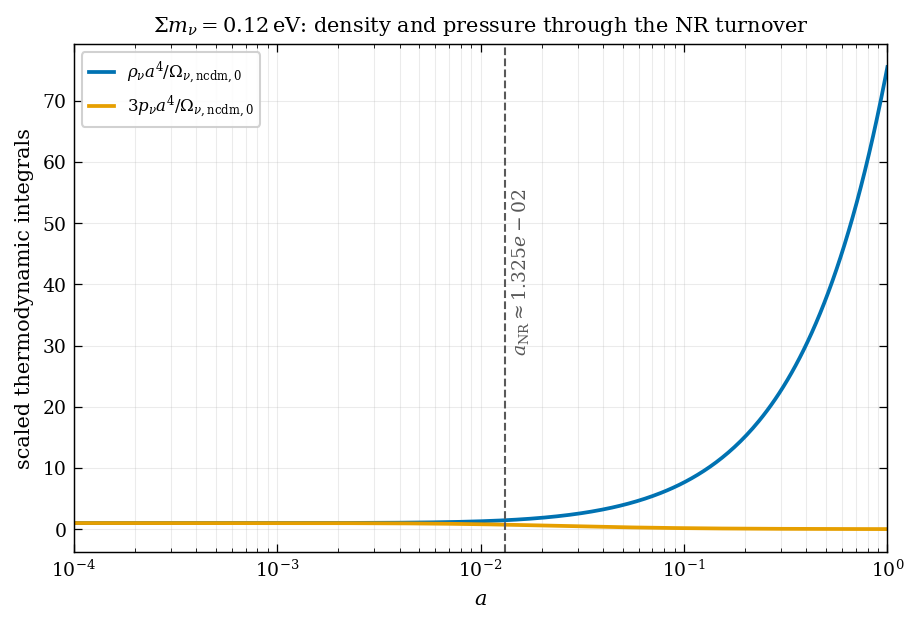
\includegraphics[width=0.78\columnwidth]{../../figures/physics_gallery/15_massive_neutrino/02_rho_p_NR_transition.png}
\caption{FB-9.2 massive-neutrino background transition for
  $\Sigma m_\nu = 0.12\,\mathrm{eV}$.  The vertical marker denotes the
  nominal non-relativistic turnover scale $a_{\rm NR}$.}
\label{fig:massive-nu-nr-transition}
\end{figure}

\subsection{FB-9.3: registry integration and the zero-mass anchor}

The systematic is introduced through the existing neutrino registry
slot, not through a new species label.  This matters for auditability:
all downstream code continues to ask for ``the neutrino background'',
while the factory dispatch decides whether that slot is massless or
massive.  The corresponding regression pin is stronger than a numerical
agreement test: with $\Sigma m_\nu = 0$ the hierarchy driver and the
full \texttt{bass/tsc} suite remain byte-identical to the LB-1 massless
path.
That short-circuit turns the massive-neutrino systematic into an
explicit opt-in perturbation rather than an ambient code-path drift.

\subsection{FB-9.4: free streaming and power suppression}

Once the neutrino species is massive, the relevant control parameter is
the free-streaming scale $k_{\rm fs}(a)$ rather than the purely
radiation-like ``free'' neutrino hierarchy.  FB-9 wires the hierarchy
through an effective $q/\epsilon$ streaming factor and recovers the
standard $k_{\rm fs}$ scaling to within the audit tolerance
\cite{LesgourguesTram2011,HuEisensteinTegmark1998}.  In practical terms,
the systematic is concentrated on modes with $k \gtrsim k_{\rm fs}$,
where the leading-order matter-power response approaches the familiar
$-8 f_\nu$ suppression.  The result is conceptually simple: the massive
neutrino is not a new dynamical sector, but a controlled deformation of
the neutrino hierarchy with a known large-$k$ footprint.

% ============================================================
\section{Phase~1.0 error budget summary}
\label{sec:err-phase10-budget}
% ============================================================

We summarise the error budget for the Phase~1.0 solver
and identify the dominant error at each level.

\begin{center}
\setlength{\tabcolsep}{5pt}
\begin{tabular}{llll}
\hline\hline
Level & Diagnostic & Phase~1.0 value & Dominant source \\
\hline
1. State-space
  & $\varepsilon_{\rm state}^{(\nu)}(\ell{=}2)$
  & $0.08$
  & Analytic $\Psi(k,\eta)$ \\[3pt]
2. Source-translation
  & $\varepsilon_{\rm Th}^{\rm lin}$
  & $\sim 10^{-3}$
  & Linearised Thomson \\[3pt]
3. Adequacy certificate
  & $\Delta_{\rm obs}^{(\gamma)}$
  & $\lesssim 10^{-8}$
  & Thomson suppression \\[3pt]
  & $\Delta_{\rm obs}^{(\nu)}$
  & $= 0$ (exact)
  & Free-streaming \\[3pt]
4. Ladder-specific
  & not evaluated
  & ---
  & Fixed truncation \\[3pt]
5. Observable
  & $\varepsilon_{C_2}$
  & $0.08$
  & $= \varepsilon_{\rm state}$ \\
\hline\hline
\end{tabular}
\end{center}

The dominant error is at Level~1 (state-space), arising
from the analytic gravitational potential.  The $\Teff$
closure itself contributes negligibly: the adequacy
certificate is $\leq 10^{-8}$ for photons and exactly
zero for neutrinos.  The source-translation error is
$\sim 10^{-3}$, three orders of magnitude below the
state-space error.  The error budget confirms that the
$\Teff$ approximation is not the bottleneck---the
gravitational potential is---and that Phase~2.0
(self-consistent Poisson) is the correct next step.

The error hierarchy also reveals a structural asymmetry
between species.  The neutrino sector contributes
$98.4\%$ of $D_2$ but introduces zero $\Teff$ error
(Levels~2--3), because free-streaming neutrinos reside
exactly on the $\Teff$ manifold.  The photon sector
contributes $1.6\%$ of $D_2$ and carries the only
nonzero $\Teff$ error, but this error is suppressed by
Thomson damping to a level that is irrelevant at any
foreseeable precision.  The $\Teff$ closure is therefore
not merely adequate but structurally optimal for the
species composition of the standard cosmological model:
the dominant species is exactly closed, and the
subdominant species is over-damped.

Before closing this chapter, we note that the five-level
hierarchy is designed to be extensible.  As the solver
programme advances through Phases~2.0--5.0
(Section~\ref{sec:solver-programme-ch9}), each level
acquires additional diagnostics---self-consistent
Poisson residuals at Level~1, nonlinear Thomson bridge
accuracy at Level~2, AniCLASS $a_{\ell m}$ comparison
at Level~5---without changing the overall structure.
The hierarchy is a framework for error accounting, not a
fixed set of numbers.


% ── Appendices and Bibliography ──────────────────────────────
% ============================================================
% appendices.tex — EXPANDED
% Part of: Tetrad-Based Departure Decomposition (Jiwon Park)
% Session S12 draft — 2026-03-30
% ============================================================

\appendix


% ============================================================
\chapter{Notation Dictionary}
\label{app:notation}
% ============================================================

We collect the principal symbols used throughout this work.
All quantities are defined relative to the common reference
congruence $u^a = n^a$
(Definition~\ref{def:common-frame}) unless otherwise noted.

\medskip

\paragraph{Spacetime and geometry.}
$(\mathcal{M}, g_{ab})$: spacetime manifold with metric
signature $(-,+,+,+)$.
$u^a$: unit timelike reference congruence ($u_a u^a = -1$).
$h_{ab} = g_{ab} + u_a u_b$: spatial projector.
$\Theta = \nabla_a u^a$: expansion scalar.
$H = \Theta/3$: Hubble rate.
$\sigma_{ab}$: shear tensor (PSTF part of $\nabla_b u_a$).
$\omega_{ab}$: vorticity tensor.
$\dot{u}_a = u^b \nabla_b u_a$: four-acceleration.
${}^3\!S_{ab}$: trace-free spatial Ricci tensor.
$\mathcal{R}$: spatial Ricci scalar.

\paragraph{Departure variables.}
$\Sigstd = \sigma_{ab}\sigma^{ab}/(6H^2)$:
standardised shear parameter.
$\Wstd = \omega_{ab}\omega^{ab}/(6H^2)$:
standardised vorticity parameter.
$\Otilt$: tilt contribution to the departure parameter.
$\Okaniso$: anisotropic curvature contribution.
$x_C = \Sigstd - \Wstd + \Otilt + \Okaniso$:
master departure parameter.
$Q_C = |x_C|/x_{\max,C}$: policy-normalized diagnostic score
(Layer~2).
$\Pi_{\rm MIO}(q_\star)$: MIO empirical diagnostic exceedance
curve over registered thresholds.
$\Pi_{\rm HTT}(q_\star)$ or $P_{\rm post}(Q>q_\star)$: HTT
model-conditional posterior exceedance, distinct from
$\Pi_{\rm MIO}$.
$\mathcal{F}_{\rm Bayes}$: legacy HTT posterior pushforward
summary; not a MIO diagnostic $F$ certificate.

\paragraph{Species-resolved quantities.}
$s \in \mathcal{K}$: kinetic species ($\gamma$, $\nu_e$,
$\bar{\nu}_e$, $\nu_x$, $\bar{\nu}_x$).
$\alpha \in \mathcal{F}$: fluid species ($b$, $c$,
$\Lambda$).
$\Theta_s(\hat{e})$: species angular temperature field.
$\eta_s(\hat{e})$: species angular fugacity field.
$T_{0,s}$: species monopole temperature.
$x_s = E_s/(k_B T_{0,s})$: dimensionless energy.
$\xi_s \in \{0, -1, +1\}$: quantum statistics (MB, FD, BE).
$\Phi_\xi(z) = 1/(e^z - \xi)$: equilibrium occupation
function.
$\mathcal{I}_n(\xi, \eta) = \int_0^\infty
x^n\,dx/(e^{x-\eta} - \xi)$: generalised thermodynamic
integral.
$g_s$: internal degeneracy.

\paragraph{Stress-energy decomposition.}
$\rho_s$, $p_s$, $q_s^a$, $\pi_s^{ab}$: species energy
density, pressure, energy flux, anisotropic stress.
$n_s$, $j_s^a$: species number density, number drift.
$Q_s^b$: energy--momentum exchange four-vector.
$R_s$: net particle creation rate.
$T^{ab}_{\rm tot} = \sum_s T_s^{ab}
+ \sum_\alpha T_\alpha^{ab}$: total stress-energy.

\paragraph{Tangency and diagnostics.}
$w_{*,s} = f_s(1 + \xi_s f_s)$: statistical weight.
$V_s = \mathrm{span}\{x_s, 1\}$: per-ray tangent space
(two-field).
$\langle g, h \rangle_{*,s}$: Fisher--entropy inner product.
$\mathcal{G}_s$: Gram matrix.
$G_{\xi,s} = C_s / w_{*,s}$: normalised collision field.
$D_{s,\geq 2}$: tangency diagnostic (off-manifold residual).

\paragraph{Transfer and evidence.}
$D_2$: CMB quadrupole power.
$E_2$: E-mode quadrupole power.
$T_2 = D_2/\Sigma^2$: calibrated transfer function.
$\ln \mathcal{B}$: log Bayes factor.
$n_{\rm live}$: number of live points (nested sampling).
$\beta$: tilt rapidity.
$\dot{\tau} = n_e \sigma_T a$: Thomson scattering rate.
$g(\eta) = \dot{\tau}\,e^{-\tau}$: visibility function.
$\tau_{\rm reio}$: reionisation optical depth.


% ============================================================
\chapter{AniCLASS Build and Validation Protocol}
\label{app:aniclass}
% ============================================================

AniCLASS~\cite{VicentePereiraPitrou2026} is the primary
external validation oracle for the Bianchi Boltzmann solver.
We document the build sequence, environment requirements, and
validation grid used in this work.


\paragraph{Build sequence.}

The code is compiled from source at
\texttt{github.com/CyrilPitrou/aniclass}.  The build
proceeds as follows:
(1)~\texttt{git clone} the repository;
(2)~\texttt{make -j4 class} to compile the C core;
(3)~\texttt{make libclass.a} to build the static library;
(4)~\texttt{pip install cython} for the Python interface;
(5)~\texttt{pip install .} from the \texttt{python/}
subdirectory.  The resulting shared library
\texttt{classy.cpython-312-x86\_64-linux-gnu.so} provides
the Python interface.


\paragraph{Environment variables.}

Two environment variables must be set at runtime:
\texttt{LD\_LIBRARY\_PATH} must include the AniCLASS build
directory (for the shared C library), and
\texttt{PYTHONPATH} must include the \texttt{python/}
subdirectory (for the \texttt{classy} module).  Failure to
set these variables produces an import error at runtime.


\paragraph{Bianchi type configuration.}

For Bianchi~VII$_h$: set \texttt{Omega\_k > 0} (open
geometry), \texttt{modes = `t, v'} (tensor and vector),
and provide \texttt{k\_output\_values} for the desired
wavenumbers.  For Bianchi~IX: set \texttt{Omega\_k < 0}
(closed geometry), \texttt{modes = `t'} (tensor only---no
vector modes are supported for type~IX), and note that the
wavenumber is determined by the curvature and cannot be
specified independently.  For Bianchi~V: recoverable as
the $\ell_s \to \infty$ limit of VII$_h$.  Bianchi~I is
excluded from AniCLASS because all supercurvature
wavenumbers $\nu_m = 0$ in the linearised formalism.


\paragraph{Validation grid.}

The cross-validation uses $15$ grid points: $12$ for
Bianchi~VII$_h$ (spanning
$\Omega_K \in \{0.001, 0.01, 0.05\}$ and
$\ell_s \in \{1, 3, 5, 10\}$) and $3$ for Bianchi~IX
($\Omega_K \in \{-0.001, -0.01, -0.05\}$).  At each grid
point, AniCLASS computes the $a_{\ell m}$ spectrum at the
fiducial Planck~2018 cosmology.  The solver's $D_2$ is
compared against the AniCLASS $\ell = 2$ power
(Section~\ref{sec:aniclass-validation}).


\paragraph{Limitations.}

AniCLASS operates strictly in the linearised regime
($\sigma/H \ll 1$), implements tensor and vector modes but
not scalar modes ($m = 0$), and does not support tilted-fluid
dynamics.  The code is valid as an oracle for Rungs~1--2 of
the solver programme (linearised, orthogonal Bianchi) but
cannot serve as a reference for the nonperturbative or
tilted-fluid regimes (Section~\ref{sec:differentiation}).


% ============================================================
\chapter{Solver Numerical Register}
\label{app:ssot}
% ============================================================

We reproduce the legacy numerical values of the Phase~1.0 solver
numerical register.  All constants derive from the SSOT
module (\texttt{ssot.py} + \texttt{obs\_defaults.json})
and are validated by \texttt{\_validate\_ssot()} at pipeline
startup.

\begin{center}
\setlength{\tabcolsep}{4pt}
\begin{tabular}{lll}
\hline\hline
Quantity & Value & Source \\
\hline
$\eta_0$ (conformal time today)
  & $14{,}174.6$~Mpc & BG-01 \\[2pt]
$z_{\rm eq}$ (matter--radiation equality)
  & $3403.1$ & BG-01 \\[2pt]
$z_*$ (Peebles recombination)
  & $1074.2$ & TC-01 \\[2pt]
$r_s$ (sound horizon)
  & $144.2$~Mpc & BG-01 \\[2pt]
$\tau(z_*)$ (optical depth at recombination)
  & $1.040$ & TC-02 \\[2pt]
$\tau_{\rm reio}$ (reionisation optical depth)
  & $0.0496$ & MT-03 \\[2pt]
$\exp(-2\tau_{\rm reio})$
  & $0.9055$ & MT-03 \\[2pt]
$D_2$(BI, $\Sigma^2 = 10^{-8}$, full)
  & $5.50 \times 10^{-5}$ & SP-04 \\[2pt]
$D_2/\Sigma^2$ (BI, linear regime)
  & $5499$ & HSR-2 \\[2pt]
$N_2/F_2$ at $\eta_*$
  & $28\times$ & SP-03 \\[2pt]
$\nu$ fraction of $D_2$
  & $98.4\%$ & HSR-3 \\[2pt]
ISW fraction of $D_2$
  & $0.6\%$ & MT-02 \\[2pt]
$E_2/F_2$ at $\eta_*$
  & $7.05\%$ & PL-01 \\[2pt]
Polarisation feedback
  & $0.006\%$ & HSR-5 \\[2pt]
Oracle $D_2$ (FLRW)
  & $931~\mu\mathrm{K}^2$ & ORC-01 v3 \\[2pt]
AniCLASS $D_2$ (FLRW)
  & $1018~\mu\mathrm{K}^2$ & VL-01 \\[2pt]
BianchiSolver speed
  & $420$~ms/eval & PR-01 \\[2pt]
\hline
\multicolumn{3}{l}{\emph{VER06 legacy numerical values}} \\[2pt]
$\ln \mathcal{B}$(FLRW$_{\rm tilt}$)
  & $+26.40$ (exact) & VER06 \\[2pt]
$\ln \mathcal{B}_{\rm tilt}$ (Route~B)
  & $+25.29 \pm 0.07$ & VER06 \\[2pt]
$\beta$
  & $1.360 \times 10^{-3}$ & VER06 \\[2pt]
$\mathcal{F}_{\rm Bayes}$
  & $0.093 \pm 0.025$ & VER06 \\[2pt]
Route~B: $C_1$
  & $1.753 \times 10^7$ & VER06 \\[2pt]
Route~B: $C_2$
  & $6.825 \times 10^5$ & VER06 \\
\hline\hline
\end{tabular}
\end{center}


% ============================================================
\chapter{Evidence Decomposition Details}
\label{app:evidence-full}
% ============================================================

Full channel-by-channel evidence decomposition tables are
available in the pipeline output JSON
(\texttt{VER06\_full\_evidence\_table.json}).
The 14-model Bayesian evidence table is reproduced in
Chapter~\ref{ch:results}.


% ============================================================
\chapter{Tilted DCP Scenario}
\label{app:DCP}
% ============================================================

The tilted dark-coincidence-problem (DCP) scenario is
analysed in Chapter~\ref{ch:results},
Section~\ref{sec:prior-sensitivity}.


% ============================================================
\chapter{The Wiltshire--Bianchi Dictionary}
\label{app:wiltshire}
% ============================================================

\begin{remark}[Quarantined content]
\label{rem:wiltshire-quarantine}
The material in this appendix is classified
\textsc{Exploratory}.  The structural obstacle described
below is unresolved, and the dictionary does not reach
the level of a working correspondence.  We include it to
document the attempt and to delineate the mathematical
barrier for future work.
\end{remark}

The Wiltshire timescape cosmology reinterprets the
observer's peculiar velocity as a gravitational-energy
gradient tilt, with the apparent acceleration arising from
differential lapse between voids and
walls~\cite{Wiltshire2007,Wiltshire2009}.  A natural
question is whether the timescape's emerging kinetic
curvature can be mapped to the Bianchi anisotropic spatial
curvature ${}^3\!S_{ab}$ that enters the departure
parameter through $\Okaniso$.

The structural obstacle is a scalar-versus-tensorial
mismatch.  The timescape's monopole-averaged kinetic
curvature $\langle \mathcal{R} \rangle_{\mathcal{D}}$ is
a scalar (one independent component), while the Bianchi
trace-free spatial curvature ${}^3\!S_{ab}$ is a rank-2
PSTF tensor (five independent components in three spatial
dimensions).  The Buchert spatial-averaging
framework~\cite{BuchertMourierRoy2020} provides the
kinematic backreaction $\mathcal{Q}_{\mathcal{D}}$ and the
averaged curvature
$\langle \mathcal{R} \rangle_{\mathcal{D}}$, but these are
scalar integrals over a spatial domain, not tensorial
quantities.

Three partial bridges exist in the literature.
The tilt sector of the departure identity maps to the
stress-energy backreaction $\mathcal{T}_{\mathcal{D}}$ in
the Buchert--Mourier--Roy generalisation, and the shear
mapping $\Omega_{\mathcal{Q}} \leftrightarrow \Sigstd$ is
structurally exact for homogeneous models.  Heinesen's
multipole cosmography framework~\cite{Heinesen2021}
decomposes observables in a covariant multipole expansion
without assuming spatial homogeneity, providing the most
natural mathematical language for a future bridge.  The
Seifert et~al.\ (2025) Pantheon+ analysis favouring
timescape over flat $\Lambda$CDM at $\sim\!3\sigma$
provides observational motivation.

A complete dictionary would require either promoting the
timescape scalar averages to a tensorial level (perhaps
through Heinesen's framework) or demoting the Bianchi
tensorial curvature to a scalar average (losing information
in the process).  Neither operation has been performed, and
the mismatch remains an open mathematical problem.


% ============================================================
\chapter{VER2 Result-Pack Crosswalk}
\label{app:ver2-crosswalk}
% ============================================================

This appendix records the exact manuscript-use contract for the
manifest-backed VER2 export family.  It is the canonical crosswalk
between generated artifacts, figure promotion, and claim-tiered prose.

% Generated by scripts/ver2_artifact_export.py
% generated from figures/paper/VER2_MANIFEST_INDEX.md (sha256:d9bdd0edcdc447c1d67a03ec908e9a85a4ba1b046108463cdf106e2cd08cdbd5)
\paragraph{VER2 figure-promotion status.}
The shared manifest audit currently reports 5 manifest-ready VER2 figure
bases and 0 blocked legacy bases. Source-conditional figures are
\texttt{fig\_ver2a\_scalar\_to\_morphology\_summary}, \texttt{fig\_ver2b\_local\_global\_discrimination\_matrix}, \texttt{fig\_ver2d\_mio\_predictive\_residuals}, but the manuscript lane remains diagnostic-only unless
native, null, covariance, and claim-tier promotion gates are separately closed.
Exploratory appendix-only figures are \texttt{fig\_ver2c\_departure\_card\_summary}, \texttt{fig\_ver2e\_validation\_campaign\_matrix}. All remaining legacy
paper figures stay blocked until a canonical manifest and a caption-tier check
are present.

% Generated by scripts/ver2_artifact_export.py
\paragraph{VER2 result-pack to manuscript map.}
Only manifest-backed result packs may be cited in the VER2 manuscript path.
The current crosswalk is:

\begin{center}
\begin{tabular}{lp{3.1cm}p{2.2cm}p{2.7cm}p{6.4cm}}
\hline
Pack & Title & Claim tier & Production status & Manuscript use \\
\hline
A & Scalar-to-morphology bridge & \texttt{conditional} & \texttt{production\_candidate} & main-text conditional morphology proxy; not a directional BiPoSH or posterior claim \\
B & Local-vs-global discrimination & \texttt{conditional} & \texttt{production\_candidate} & appendix-only diagnostic on local-vs-global degeneracy; not posterior odds \\
C & Departure cards & \texttt{exploratory} & \texttt{diagnostic\_only} & appendix-only descriptive departure card; not certified filling or geometry validation \\
D & MIO certificates & \texttt{conditional} & \texttt{production\_candidate} & main-text conditional residual-atlas check; not truth certification or posterior evidence \\
E & Equivalence and validation classes & \texttt{exploratory} & \texttt{diagnostic\_only} & appendix-only validation coverage matrix; warn campaigns remain no-claim gates \\
\hline
\end{tabular}
\end{center}

% Generated by scripts/ver2_artifact_export.py
\paragraph{VER2 validation ceiling.}
The executable VER2 registry currently contains 6 campaigns and
9 theorem anchors; campaign states are pass=2, warn=4. The shared
status snapshot reports 0 production-validated rows. Warn-grade
campaigns therefore remain explicit no-claim gates: they document coverage and
hostile-audit provenance, but they do not by themselves validate a scientific claim.


The main text promotes only the two conditional figures
(the conditioned legacy figure gallery in Appendix~\ref{app:conditioned-legacy-figure-gallery}) because those are the only
current packs that can carry a bounded scientific statement without
crossing the claim-tier ceiling.  The three figures below are retained
as appendix-only diagnostics.

\clearpage
% Auto-generated by scripts/build_expanded_manuscript_figure_suite.py --phase aggressive
\chapter{Conditioned Legacy Figure Gallery}
\label{app:conditioned-legacy-figure-gallery}

This appendix includes legacy figures only after adding explicit condition, provenance, and claim-ceiling sidecars.  These figures are appendix-only diagnostics.  They are not current production results, not native low-ell outputs, and not Bianchi family-ID or geometry-detection evidence.

\captionsetup{hypcap=false}

\clearpage
\begin{center}
\centering
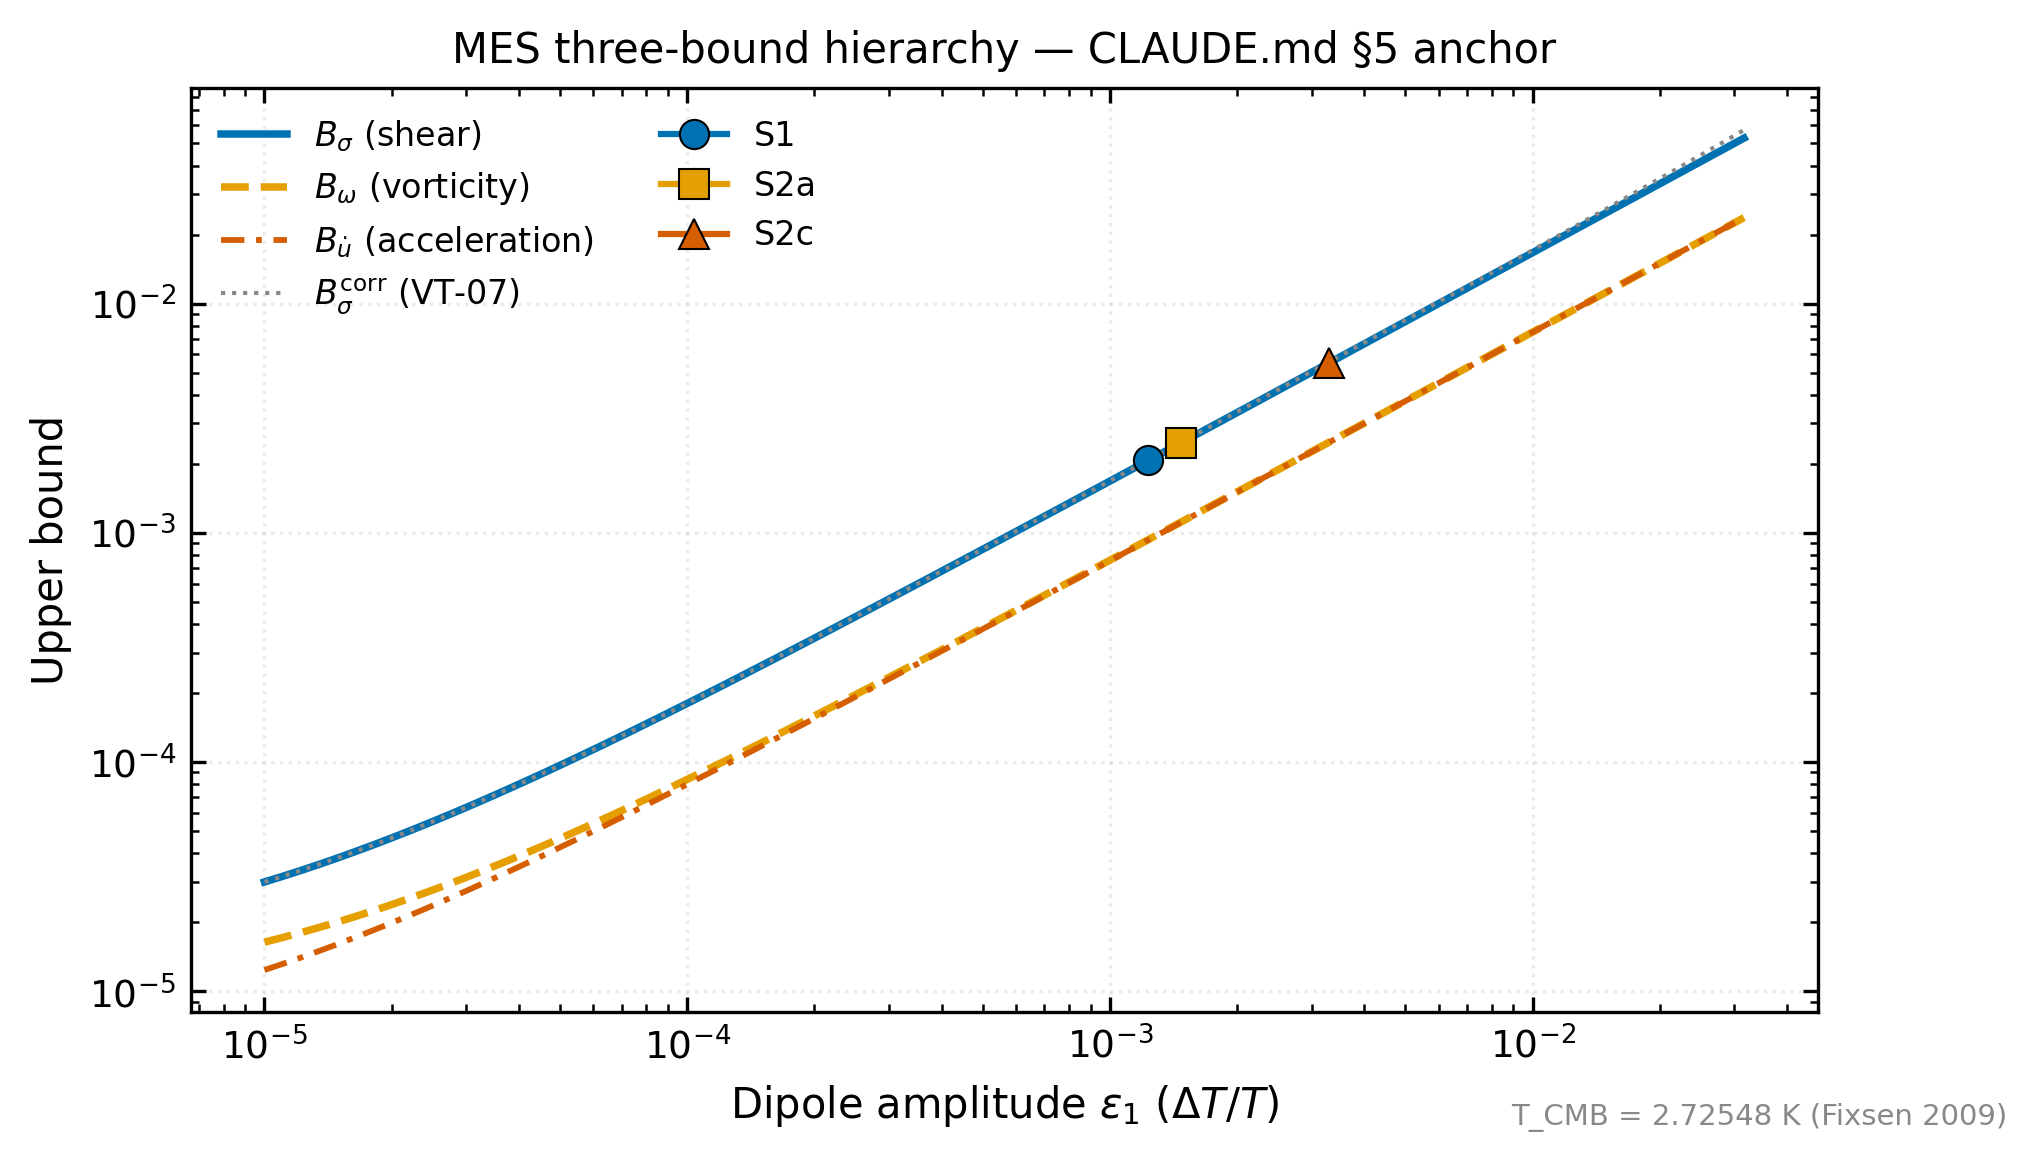
\includegraphics[width=0.82\textwidth,height=0.58\textheight,keepaspectratio]{conditioned_legacy/parallel-track__fig_01_mes_three_bounds}
\captionof{figure}{Conditioned legacy diagnostic: mes three bounds. Condition: parallel-track prior context. See sidecar manifest for provenance and caveats; appendix-only, not native-transfer or family-ID evidence.}
\label{fig:conditioned-legacy-parallel-track-fig-01-mes-three-bounds}
\end{center}

\clearpage
\begin{center}
\centering
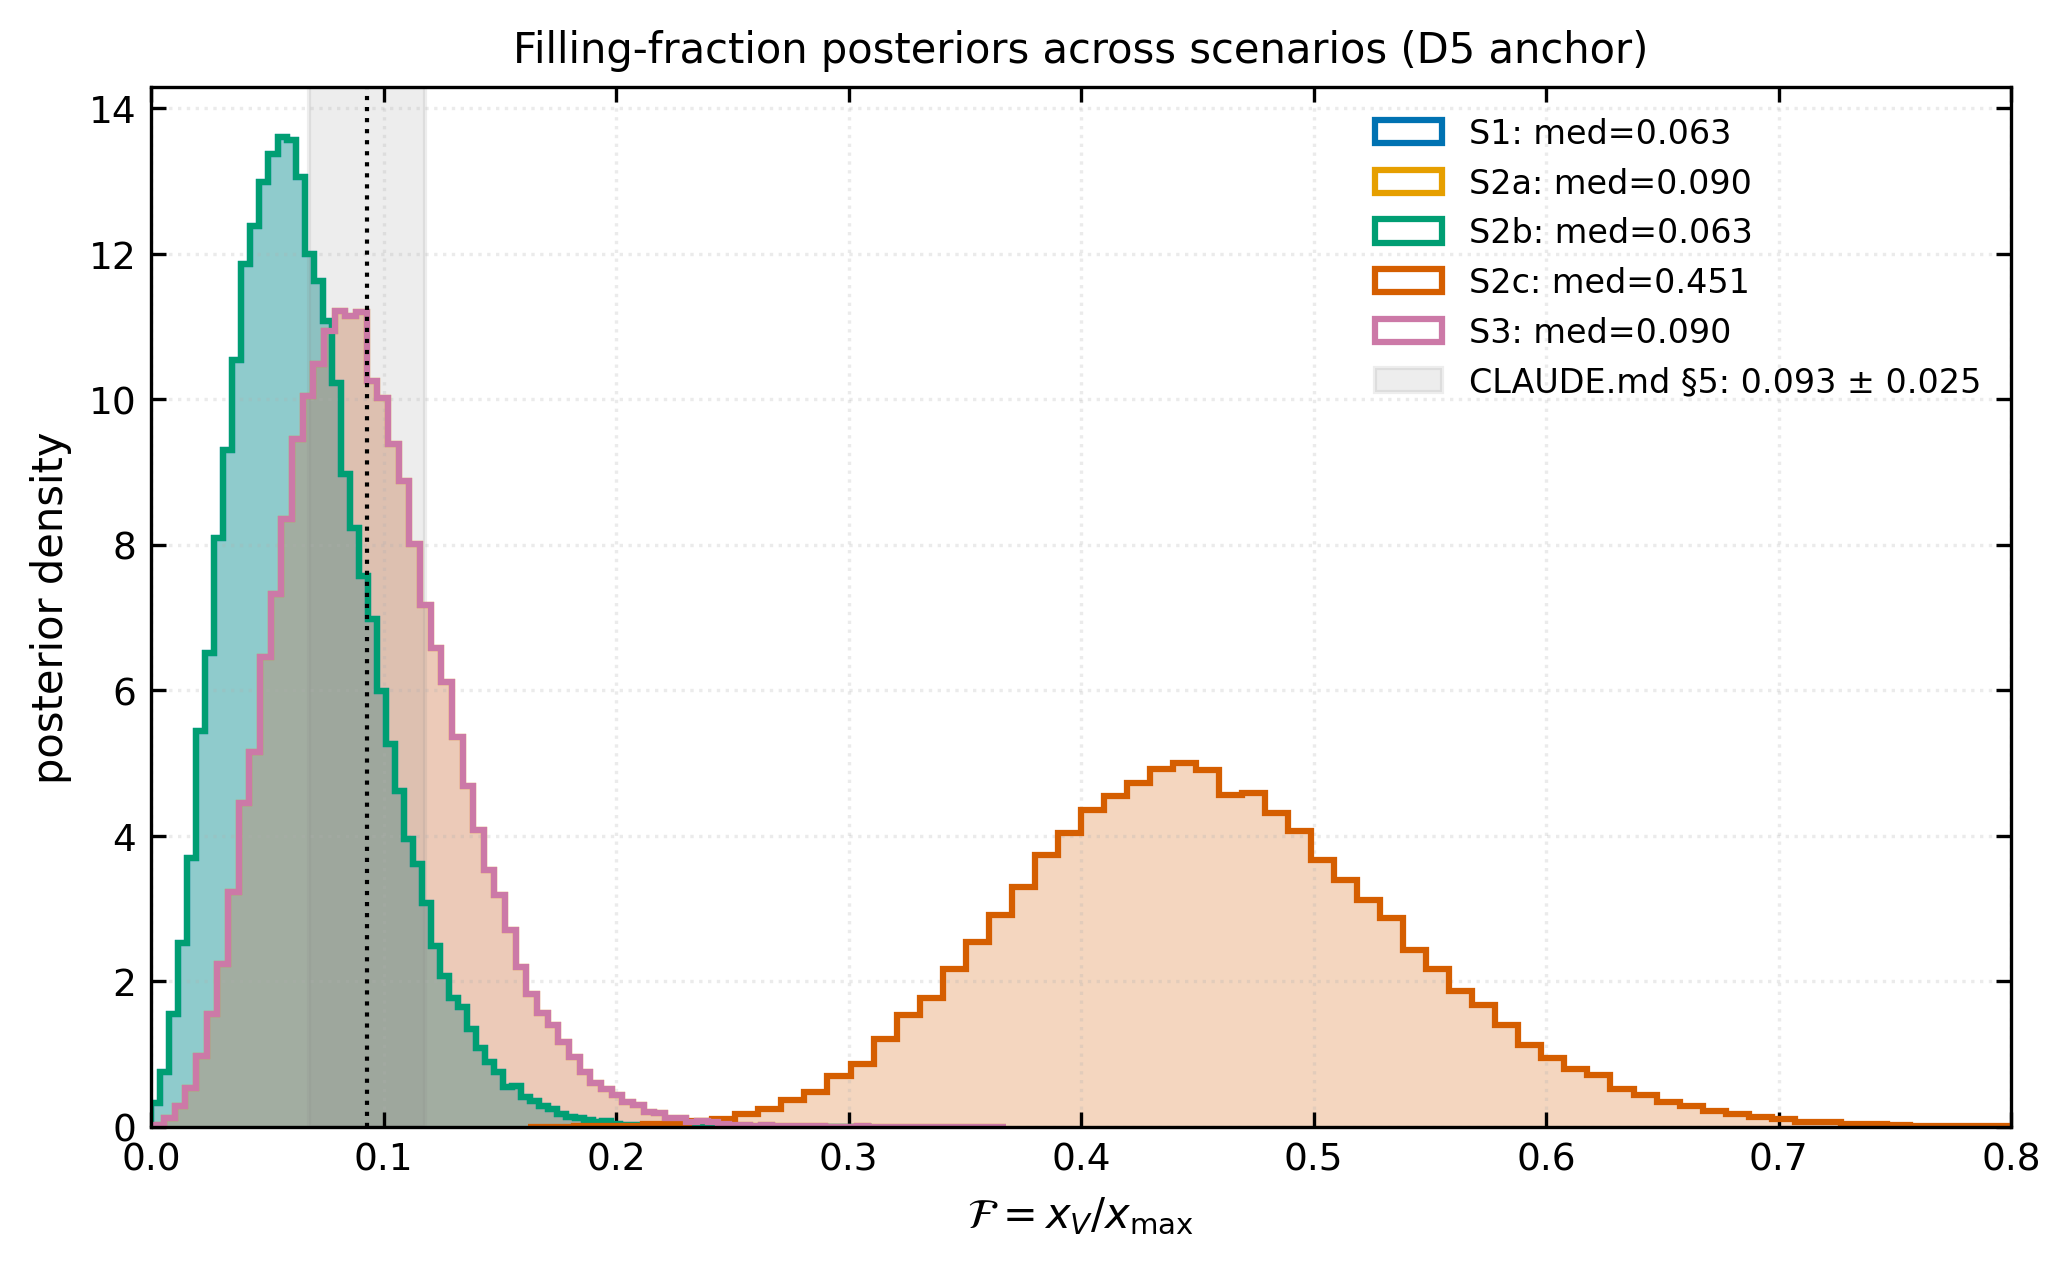
\includegraphics[width=0.82\textwidth,height=0.58\textheight,keepaspectratio]{conditioned_legacy/parallel-track__fig_05_filling_fraction_scenarios}
\captionof{figure}{Conditioned legacy diagnostic: filling fraction scenarios. Condition: parallel-track prior context. See sidecar manifest for provenance and caveats; appendix-only, not native-transfer or family-ID evidence.}
\label{fig:conditioned-legacy-parallel-track-fig-05-filling-fraction-scenarios}
\end{center}

\clearpage
\begin{center}
\centering
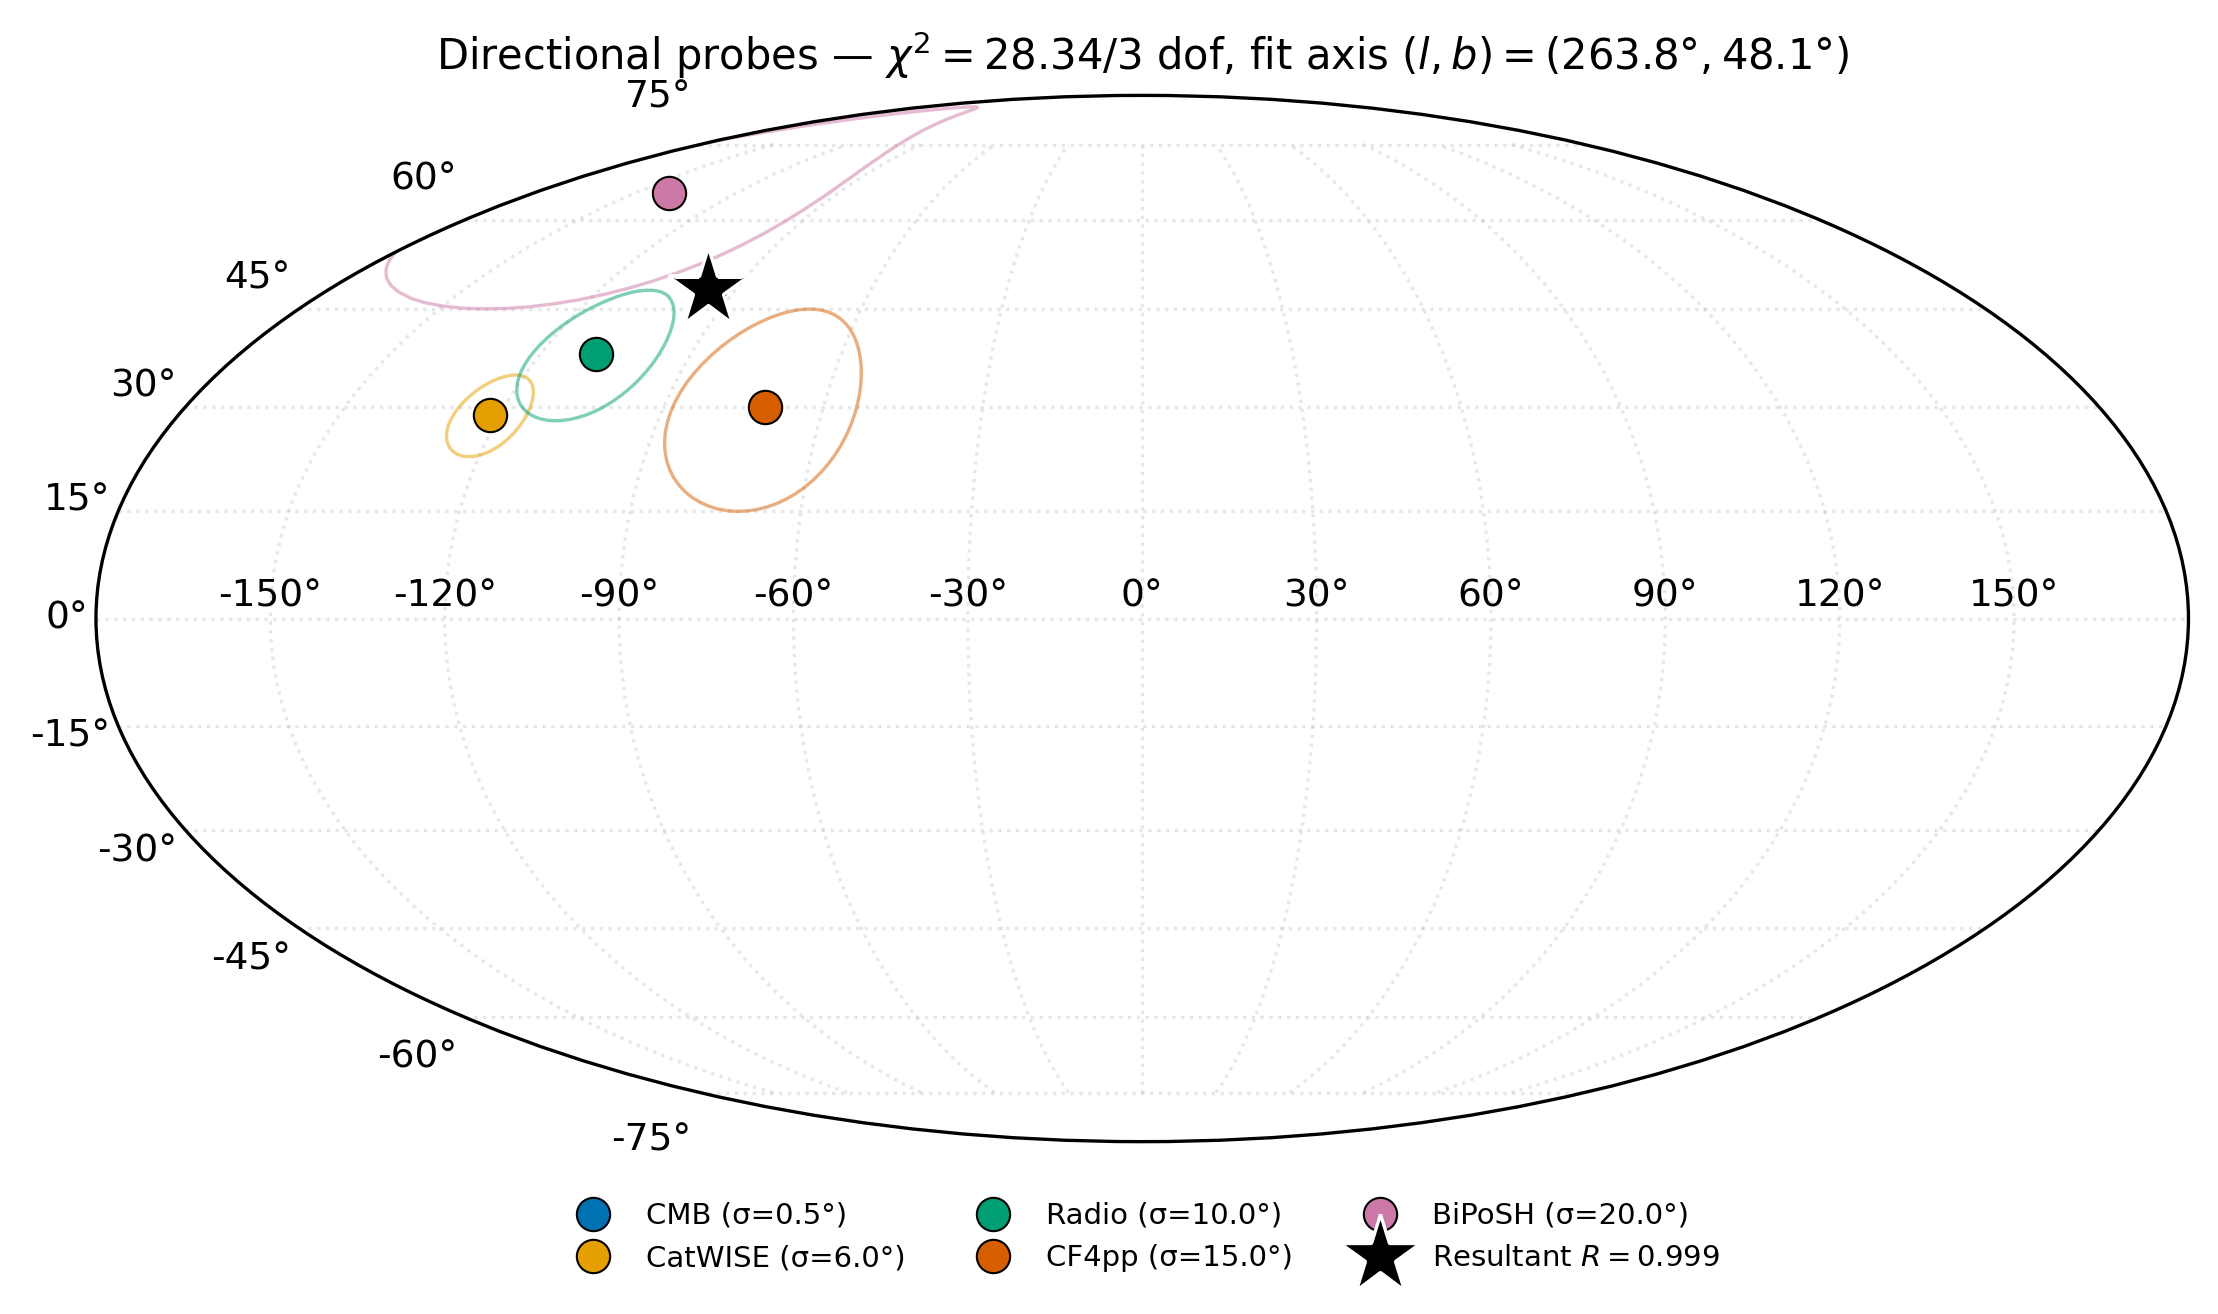
\includegraphics[width=0.82\textwidth,height=0.58\textheight,keepaspectratio]{conditioned_legacy/parallel-track__fig_06_directional_probes_mollweide}
\captionof{figure}{Conditioned legacy diagnostic: directional probes mollweide. Condition: parallel-track prior context. See sidecar manifest for provenance and caveats; appendix-only, not native-transfer or family-ID evidence.}
\label{fig:conditioned-legacy-parallel-track-fig-06-directional-probes-mollweide}
\end{center}

\clearpage
\begin{center}
\centering
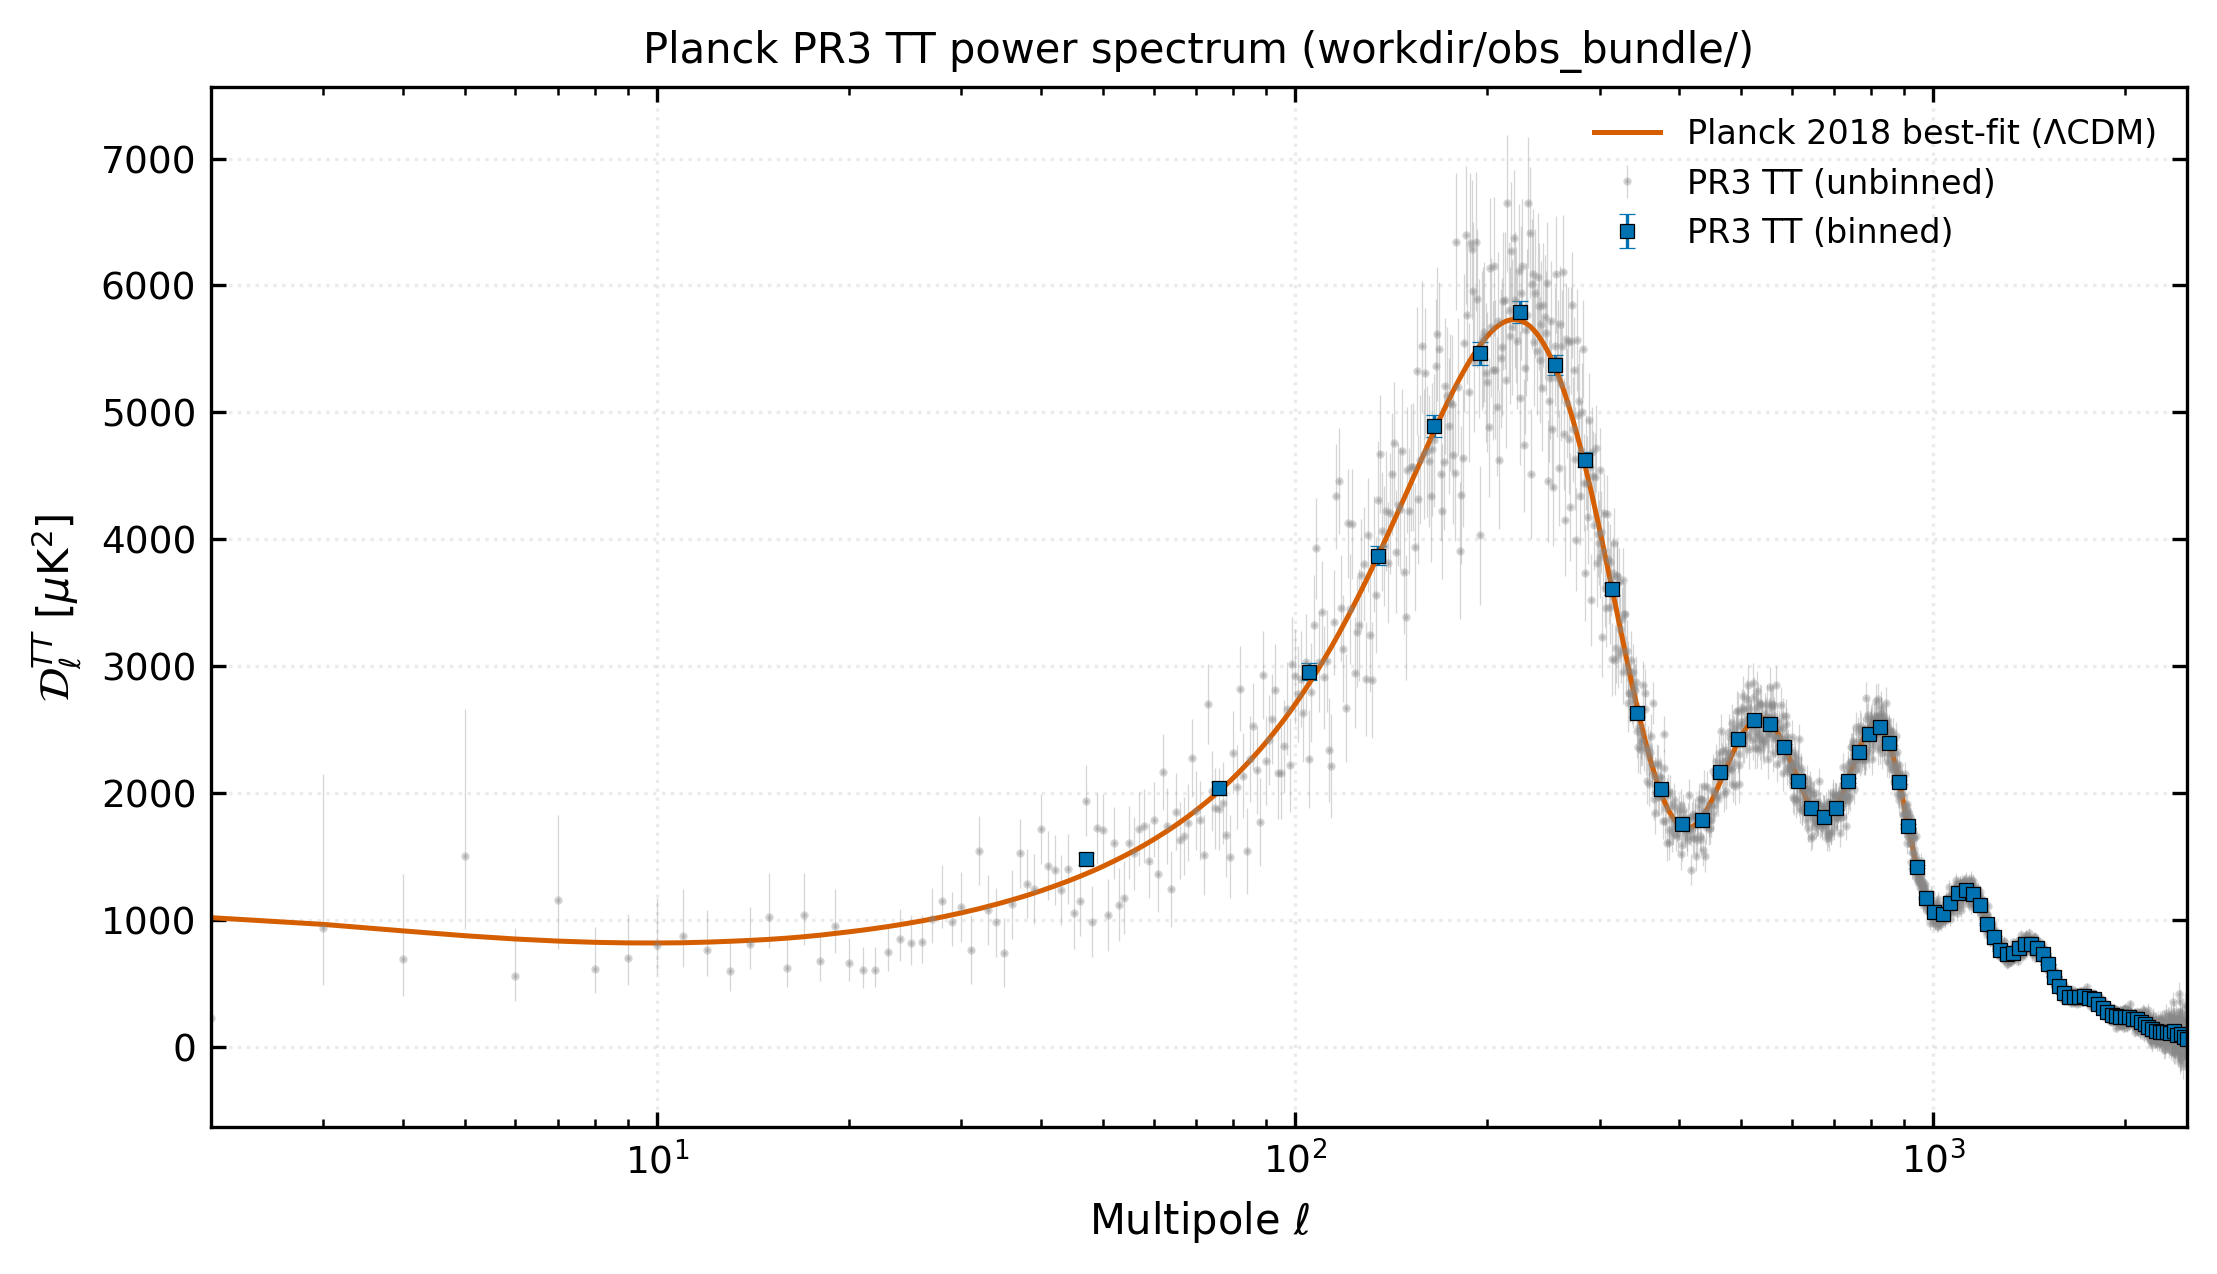
\includegraphics[width=0.82\textwidth,height=0.58\textheight,keepaspectratio]{conditioned_legacy/parallel-track__fig_07_planck_pr3_tt}
\captionof{figure}{Conditioned legacy diagnostic: planck pr3 tt. Condition: parallel-track prior context. See sidecar manifest for provenance and caveats; appendix-only, not native-transfer or family-ID evidence.}
\label{fig:conditioned-legacy-parallel-track-fig-07-planck-pr3-tt}
\end{center}

\clearpage
\begin{center}
\centering
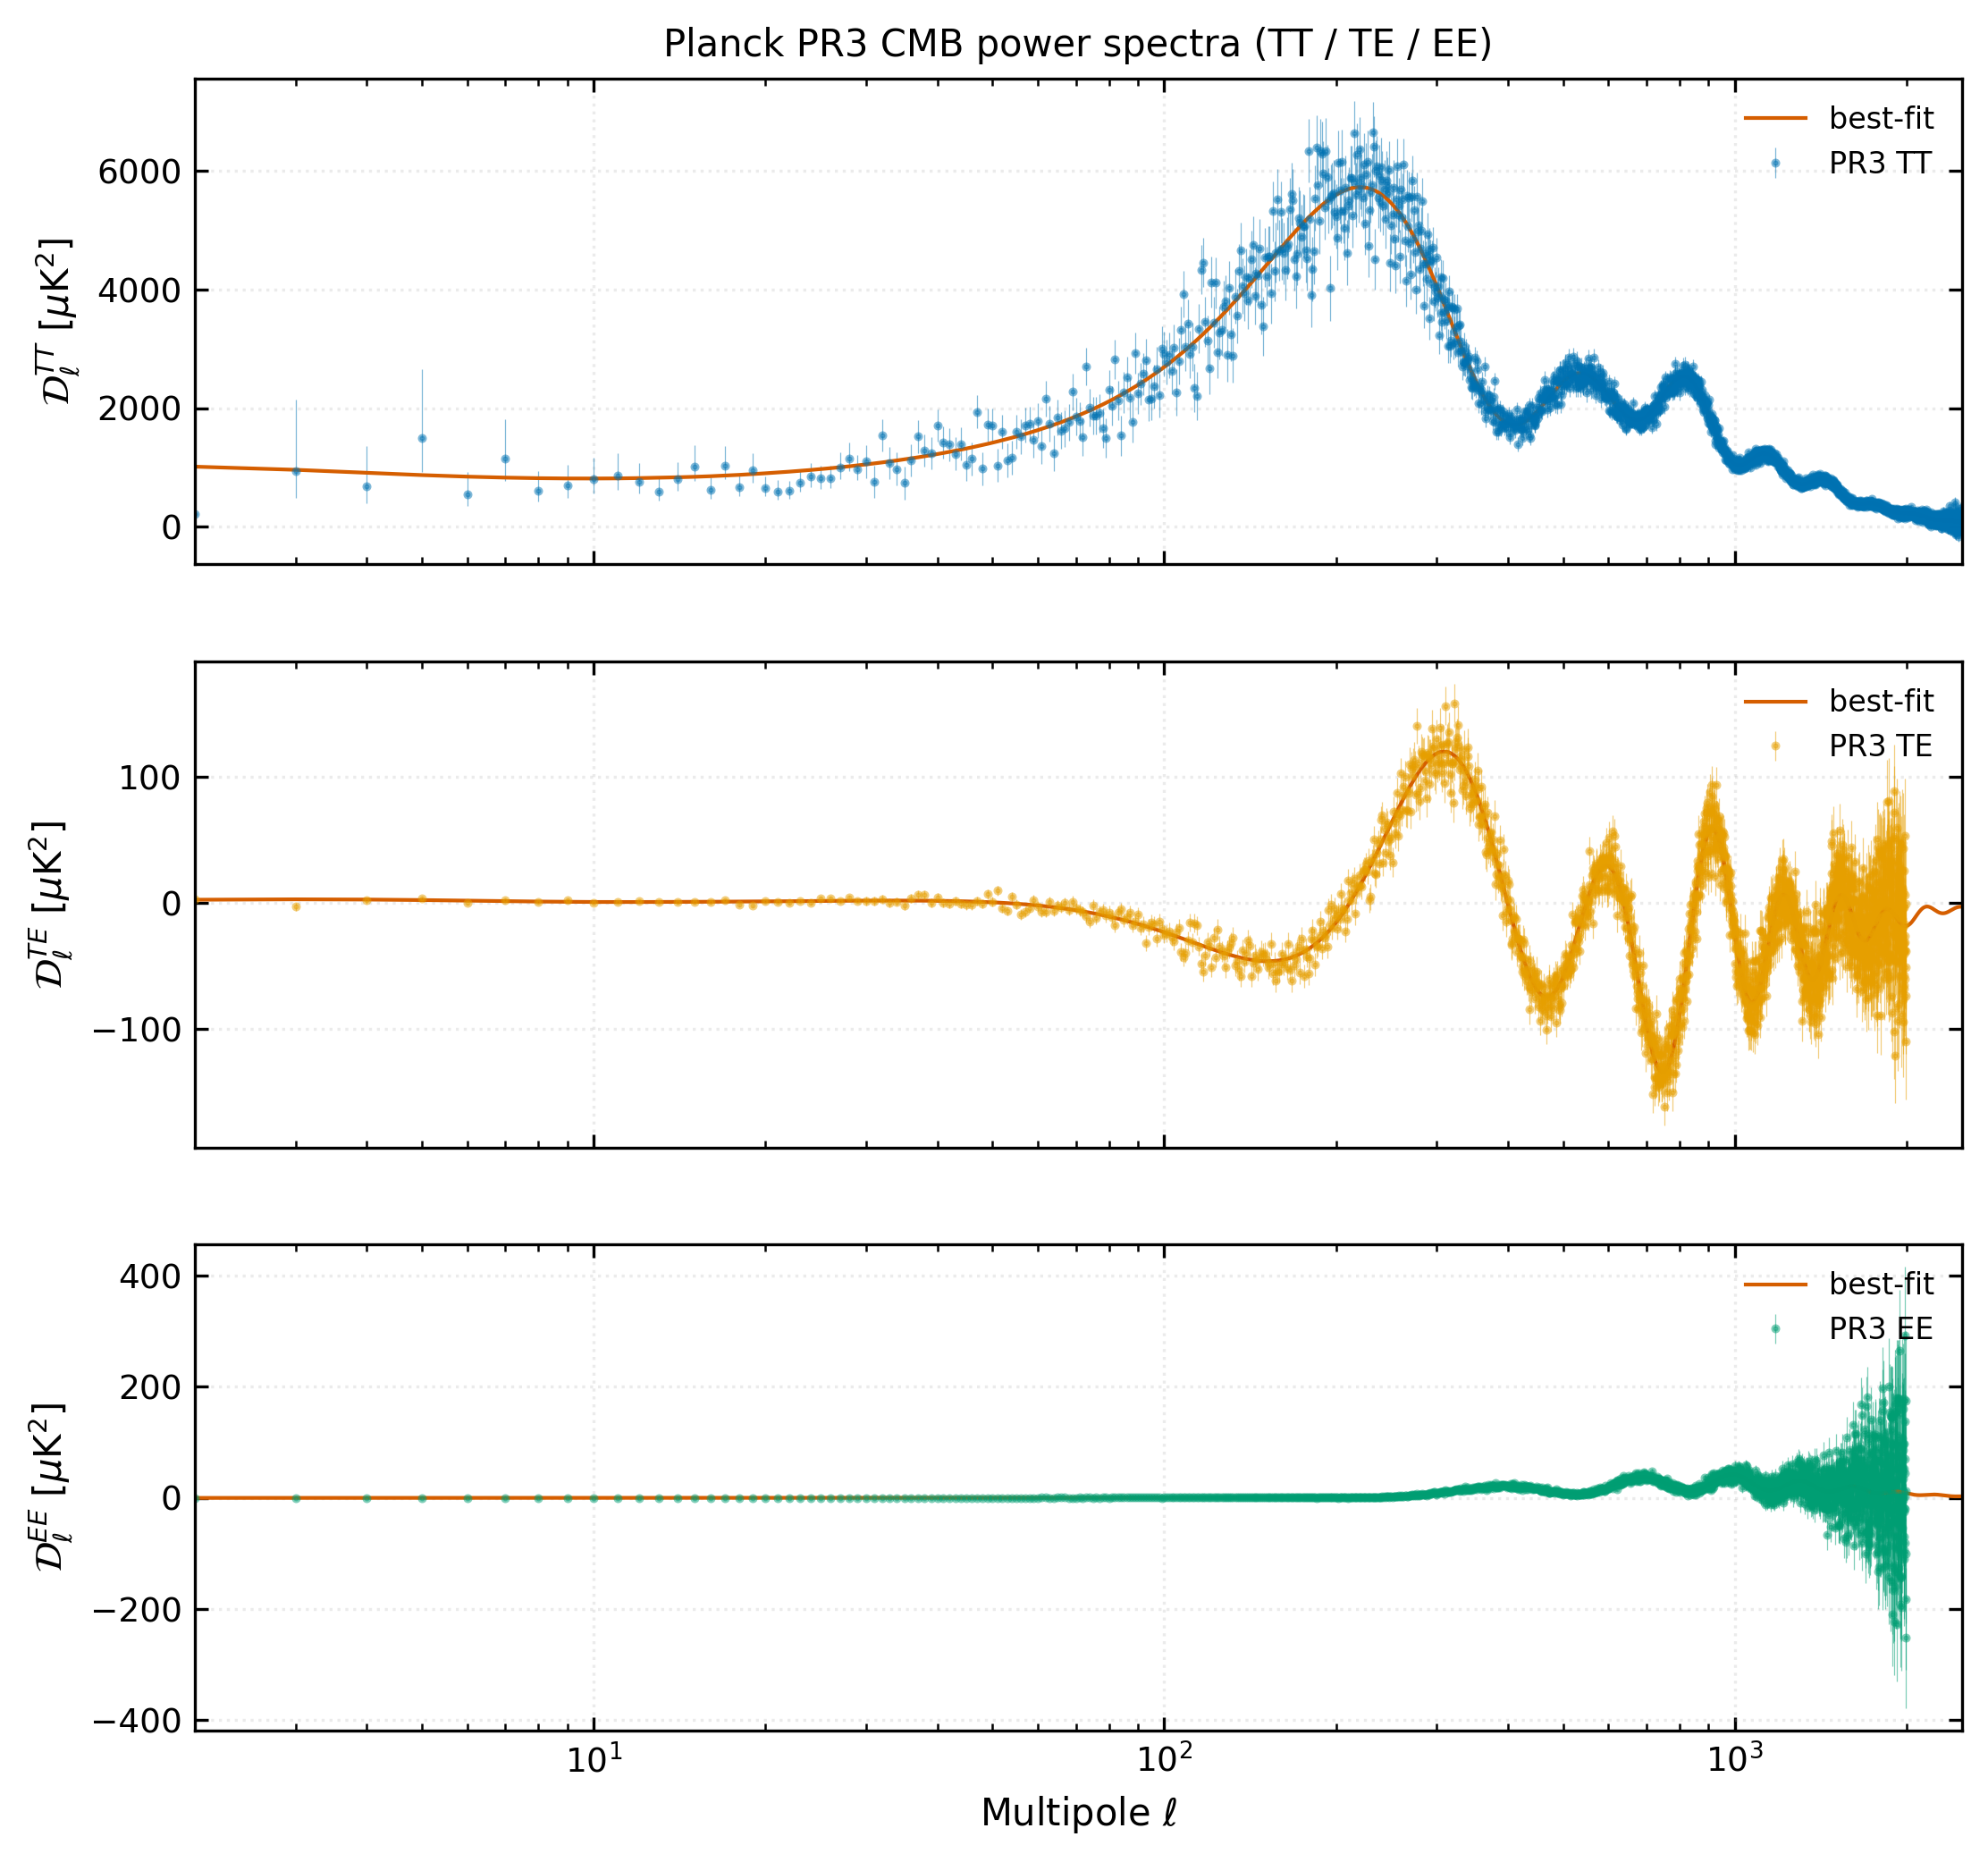
\includegraphics[width=0.82\textwidth,height=0.58\textheight,keepaspectratio]{conditioned_legacy/parallel-track__fig_08_planck_pr3_tt_te_ee}
\captionof{figure}{Conditioned legacy diagnostic: planck pr3 tt te ee. Condition: parallel-track prior context. See sidecar manifest for provenance and caveats; appendix-only, not native-transfer or family-ID evidence.}
\label{fig:conditioned-legacy-parallel-track-fig-08-planck-pr3-tt-te-ee}
\end{center}

\clearpage
\begin{center}
\centering
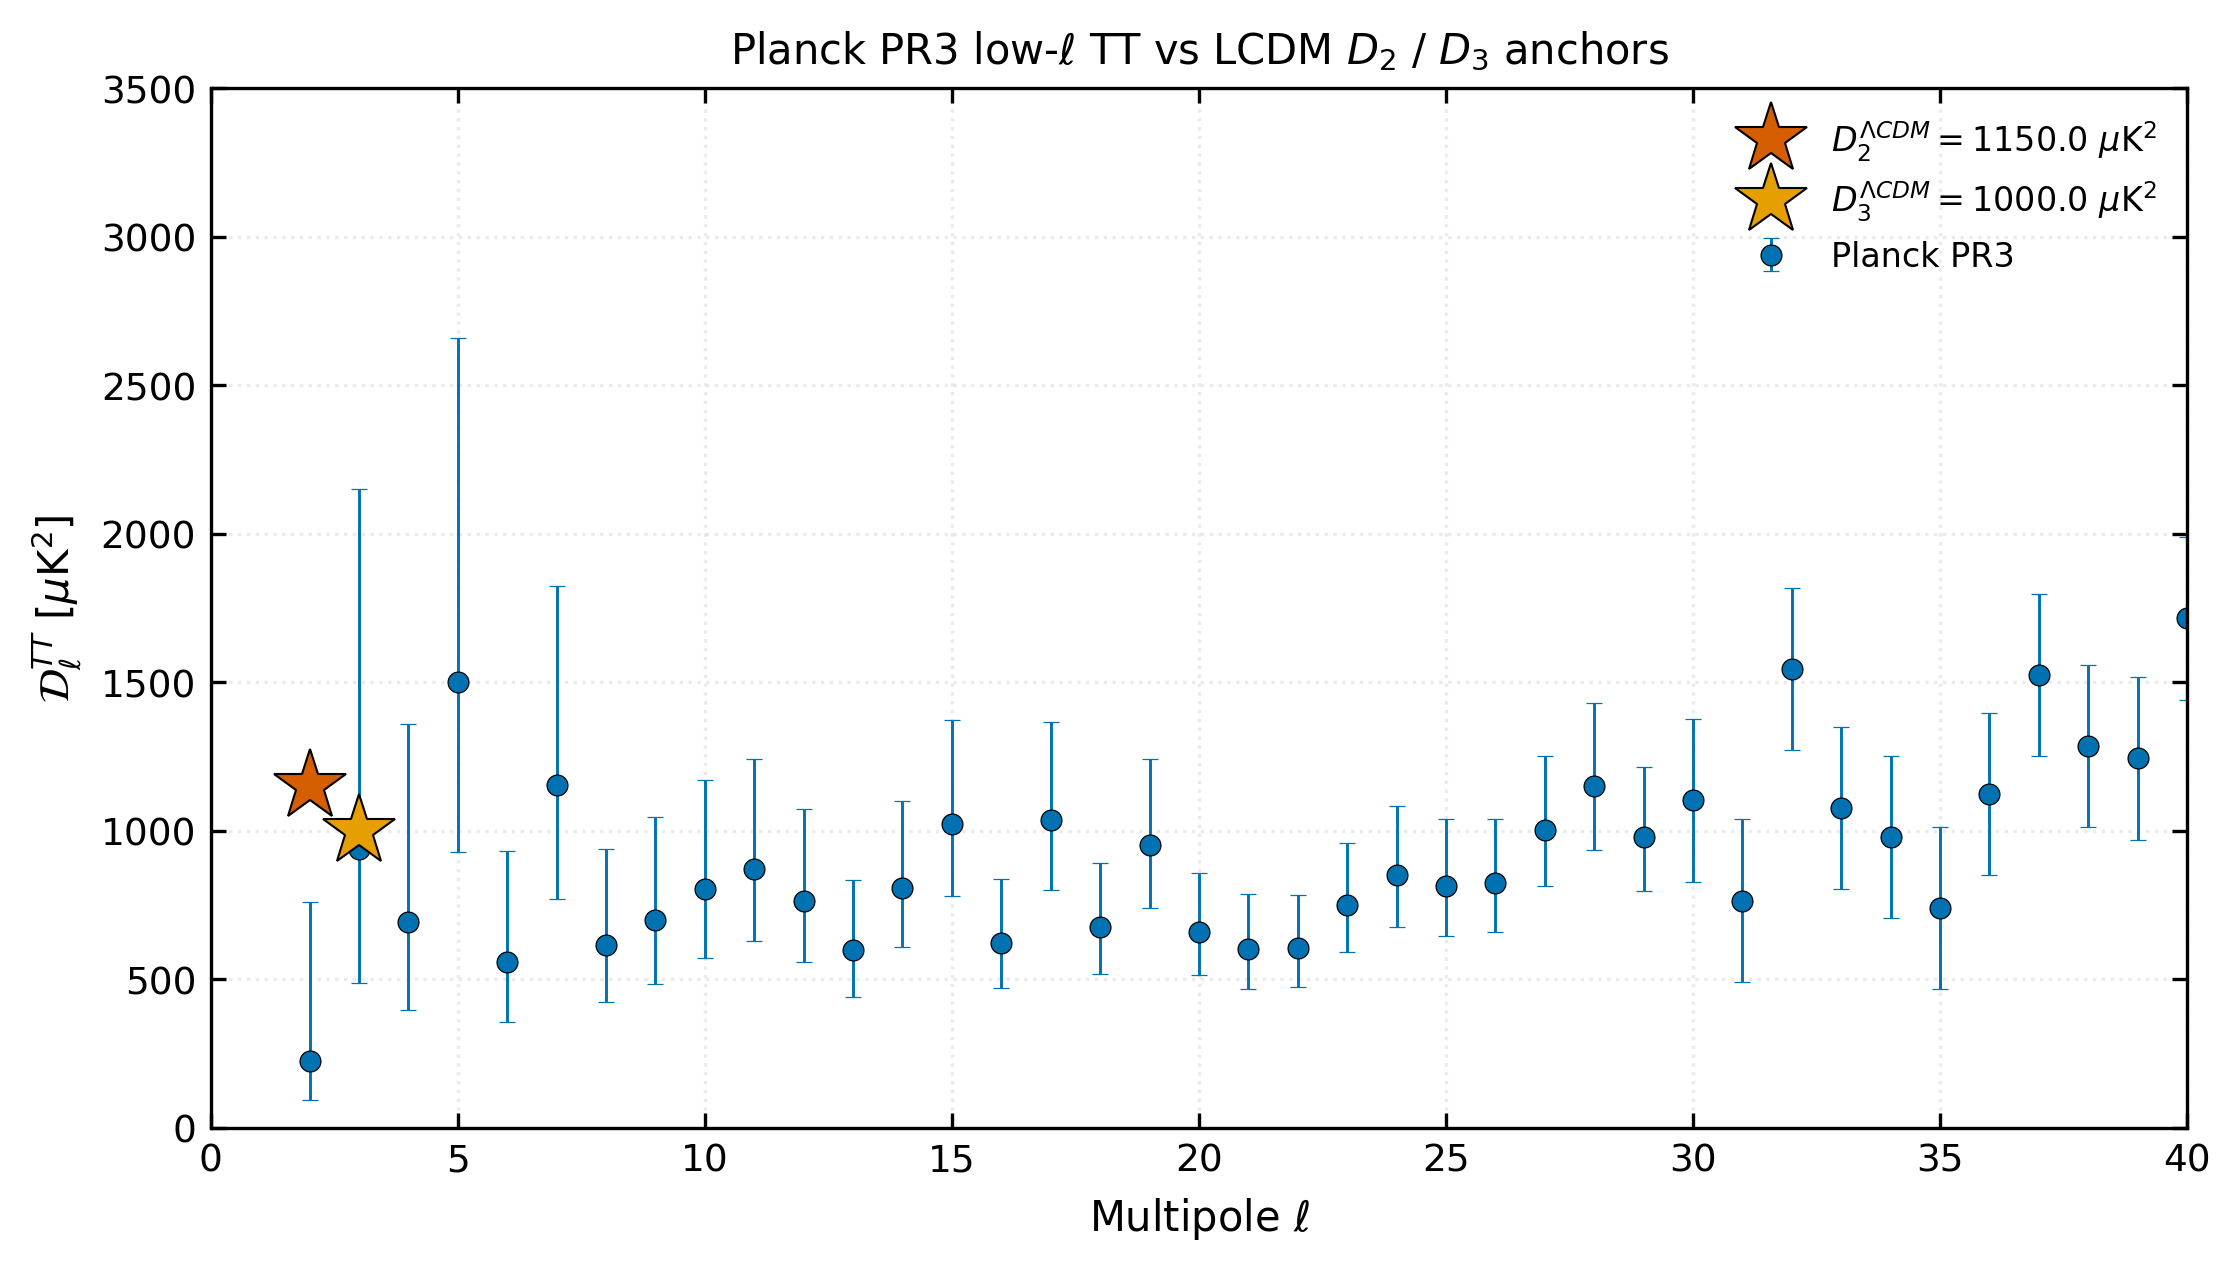
\includegraphics[width=0.82\textwidth,height=0.58\textheight,keepaspectratio]{conditioned_legacy/parallel-track__fig_09_planck_lowell_envelope}
\captionof{figure}{Conditioned legacy diagnostic: planck lowell envelope. Condition: parallel-track prior context. See sidecar manifest for provenance and caveats; appendix-only, not native-transfer or family-ID evidence.}
\label{fig:conditioned-legacy-parallel-track-fig-09-planck-lowell-envelope}
\end{center}

\clearpage
\begin{center}
\centering
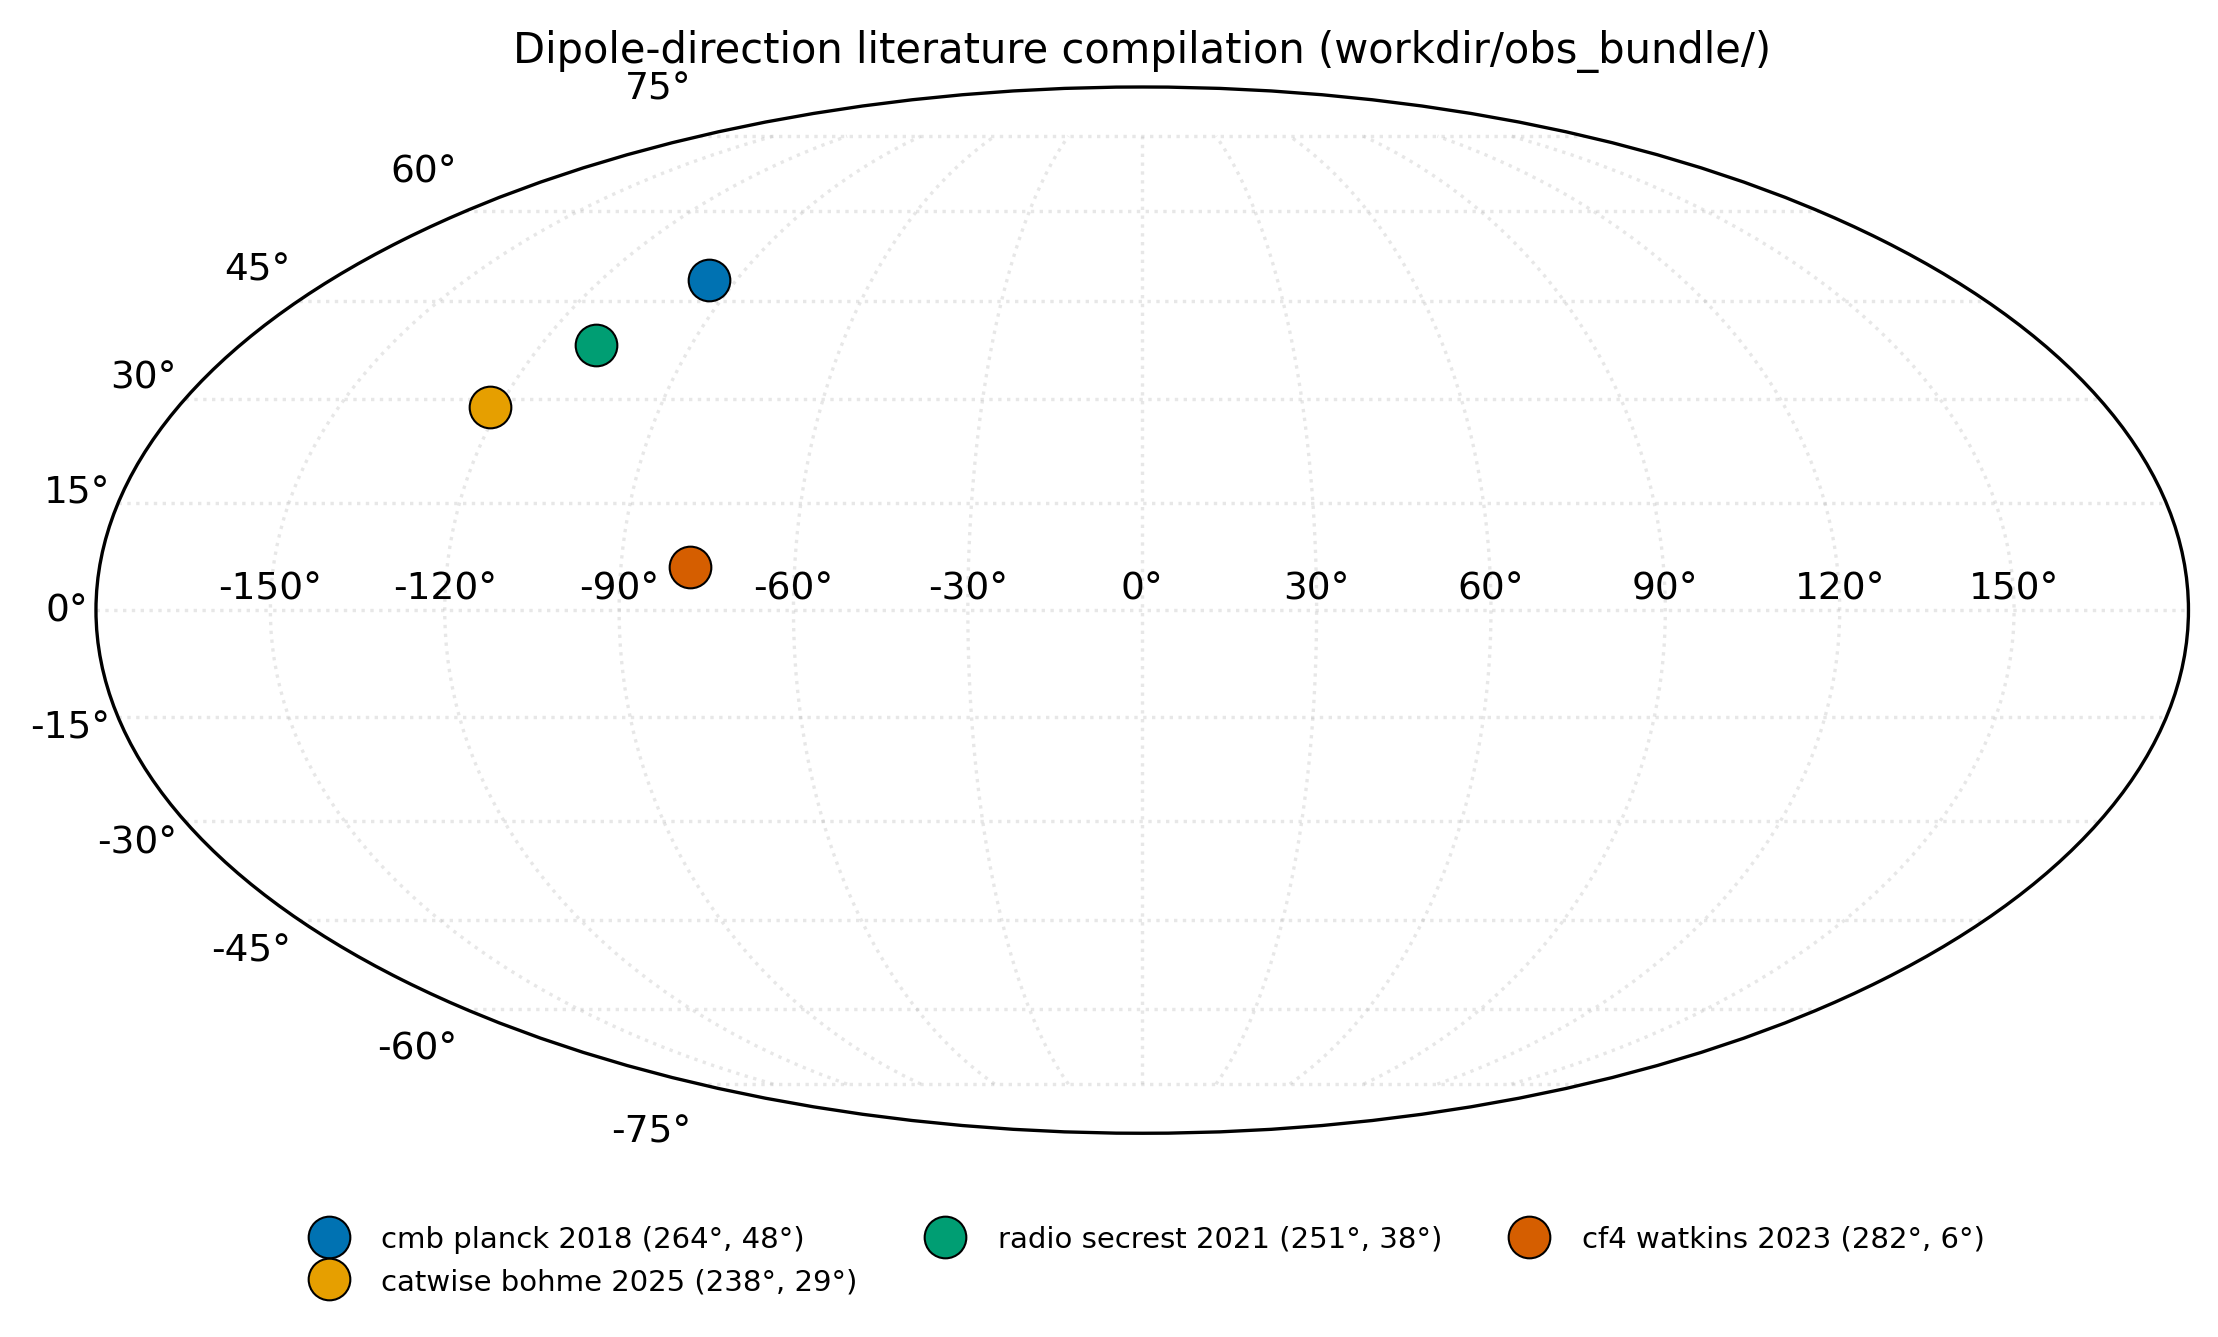
\includegraphics[width=0.82\textwidth,height=0.58\textheight,keepaspectratio]{conditioned_legacy/parallel-track__fig_11_dipole_direction_comparison}
\captionof{figure}{Conditioned legacy diagnostic: dipole direction comparison. Condition: parallel-track prior context. See sidecar manifest for provenance and caveats; appendix-only, not native-transfer or family-ID evidence.}
\label{fig:conditioned-legacy-parallel-track-fig-11-dipole-direction-comparison}
\end{center}

\clearpage
\begin{center}
\centering
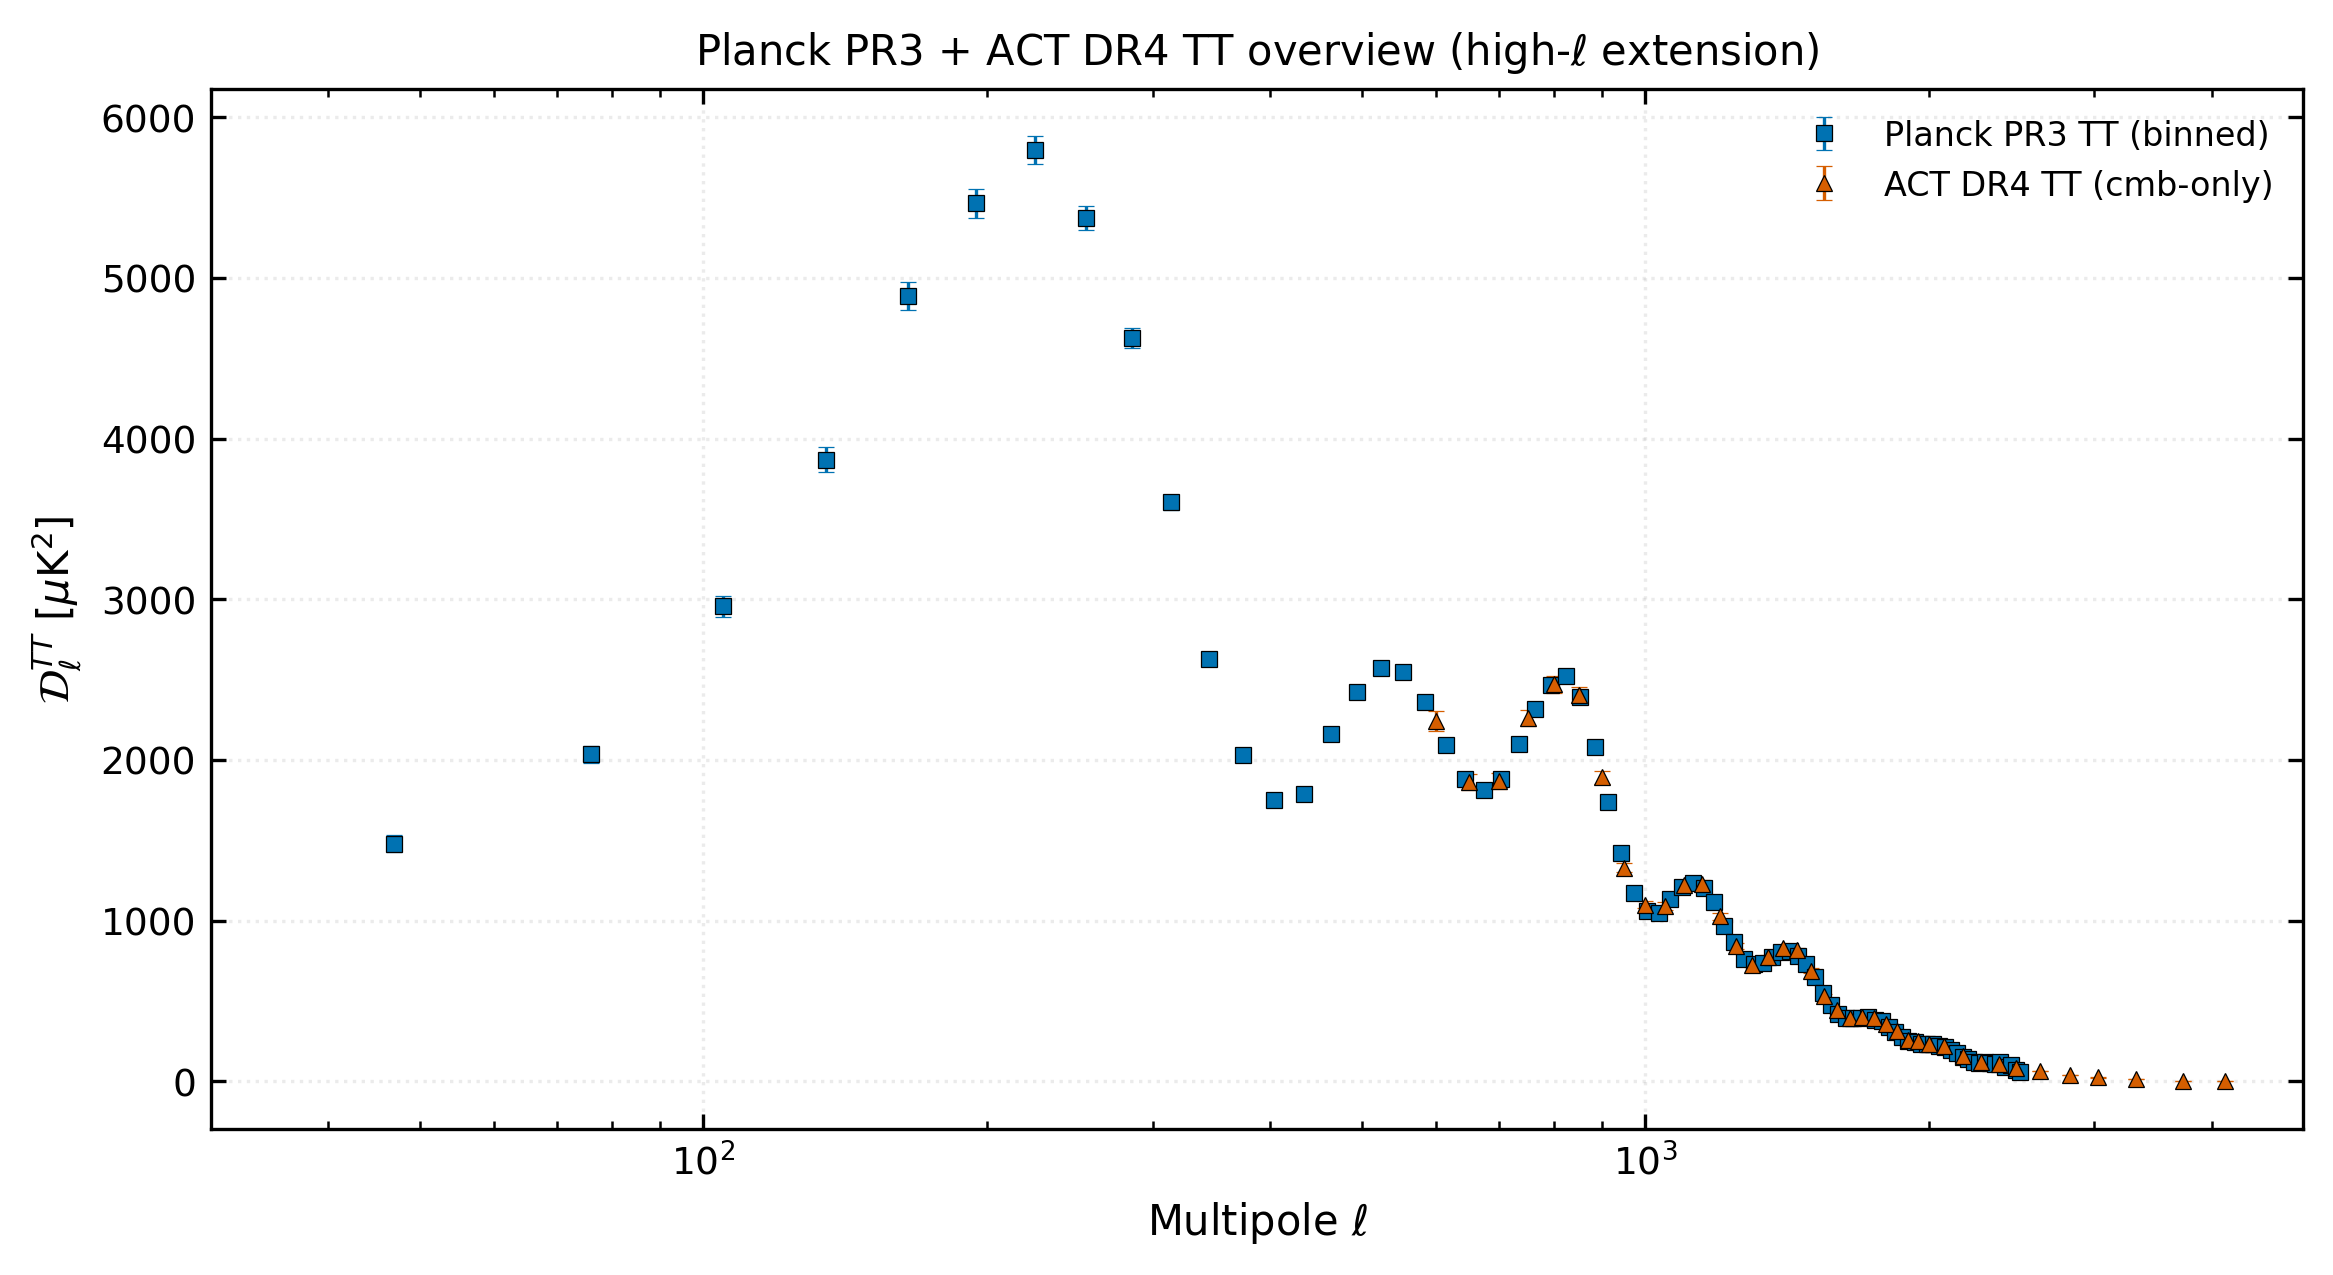
\includegraphics[width=0.82\textwidth,height=0.58\textheight,keepaspectratio]{conditioned_legacy/parallel-track__fig_12_planck_act_dr4_combined}
\captionof{figure}{Conditioned legacy diagnostic: planck act dr4 combined. Condition: parallel-track prior context. See sidecar manifest for provenance and caveats; appendix-only, not native-transfer or family-ID evidence.}
\label{fig:conditioned-legacy-parallel-track-fig-12-planck-act-dr4-combined}
\end{center}

\clearpage
\begin{center}
\centering
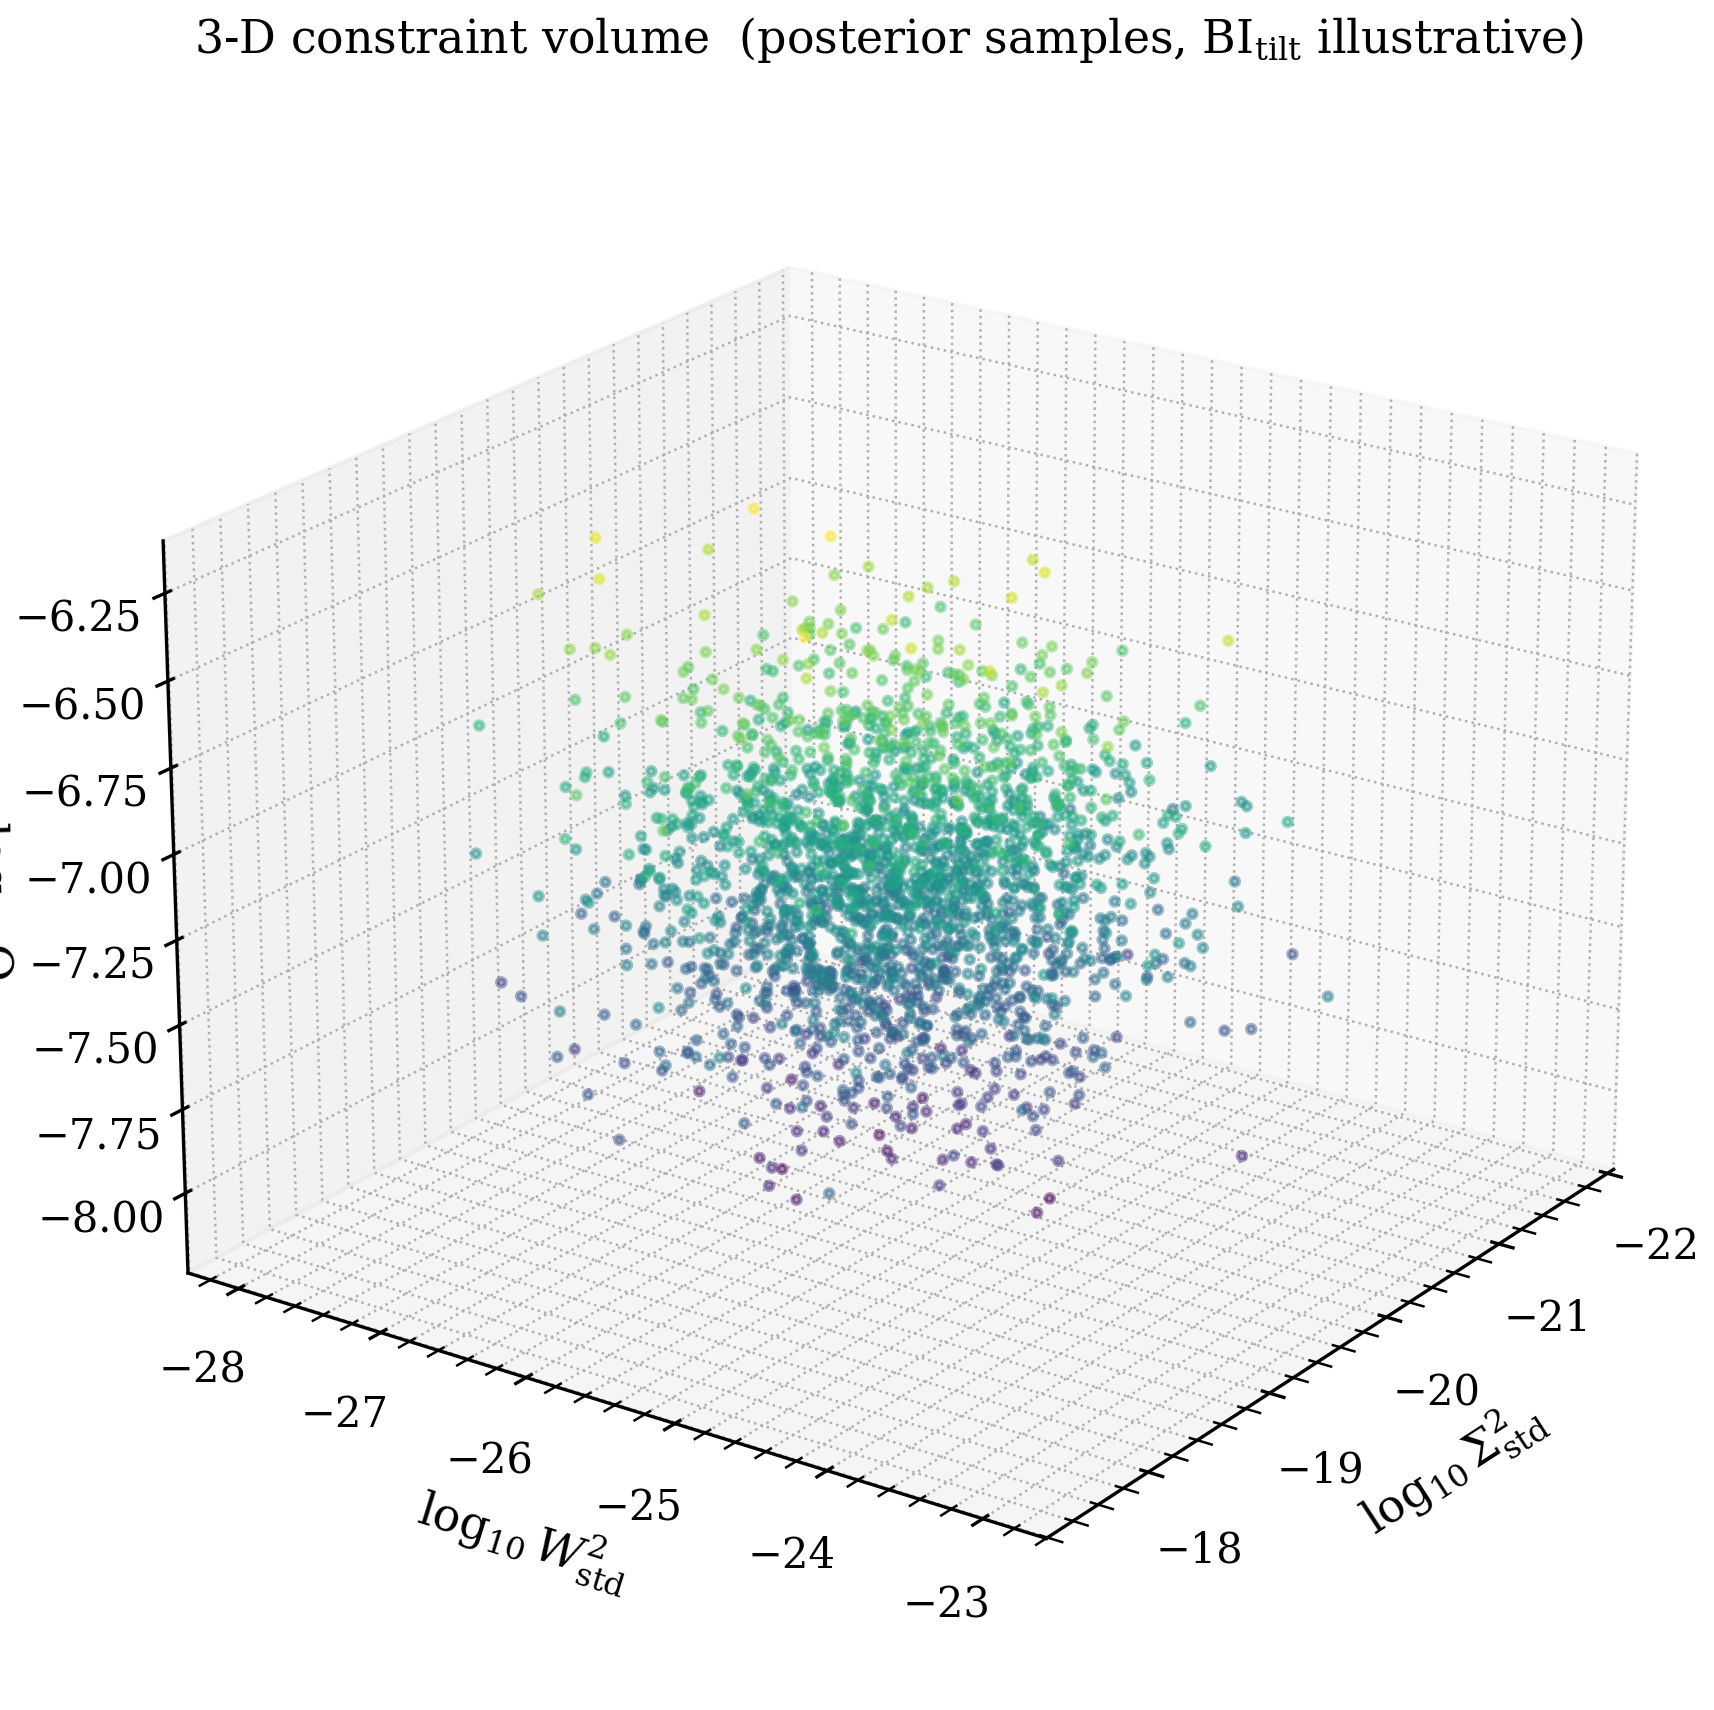
\includegraphics[width=0.82\textwidth,height=0.58\textheight,keepaspectratio]{conditioned_legacy/quarantined-legacy-root-sources__fig_3D_constraint_volume}
\captionof{figure}{Conditioned legacy diagnostic: 3D constraint volume. Condition: legacy manuscript-generator assumptions. See sidecar manifest for provenance and caveats; appendix-only, not native-transfer or family-ID evidence.}
\label{fig:conditioned-legacy-quarantined-legacy-root-sources-fig-3d-constraint-volume}
\end{center}

\clearpage
\begin{center}
\centering
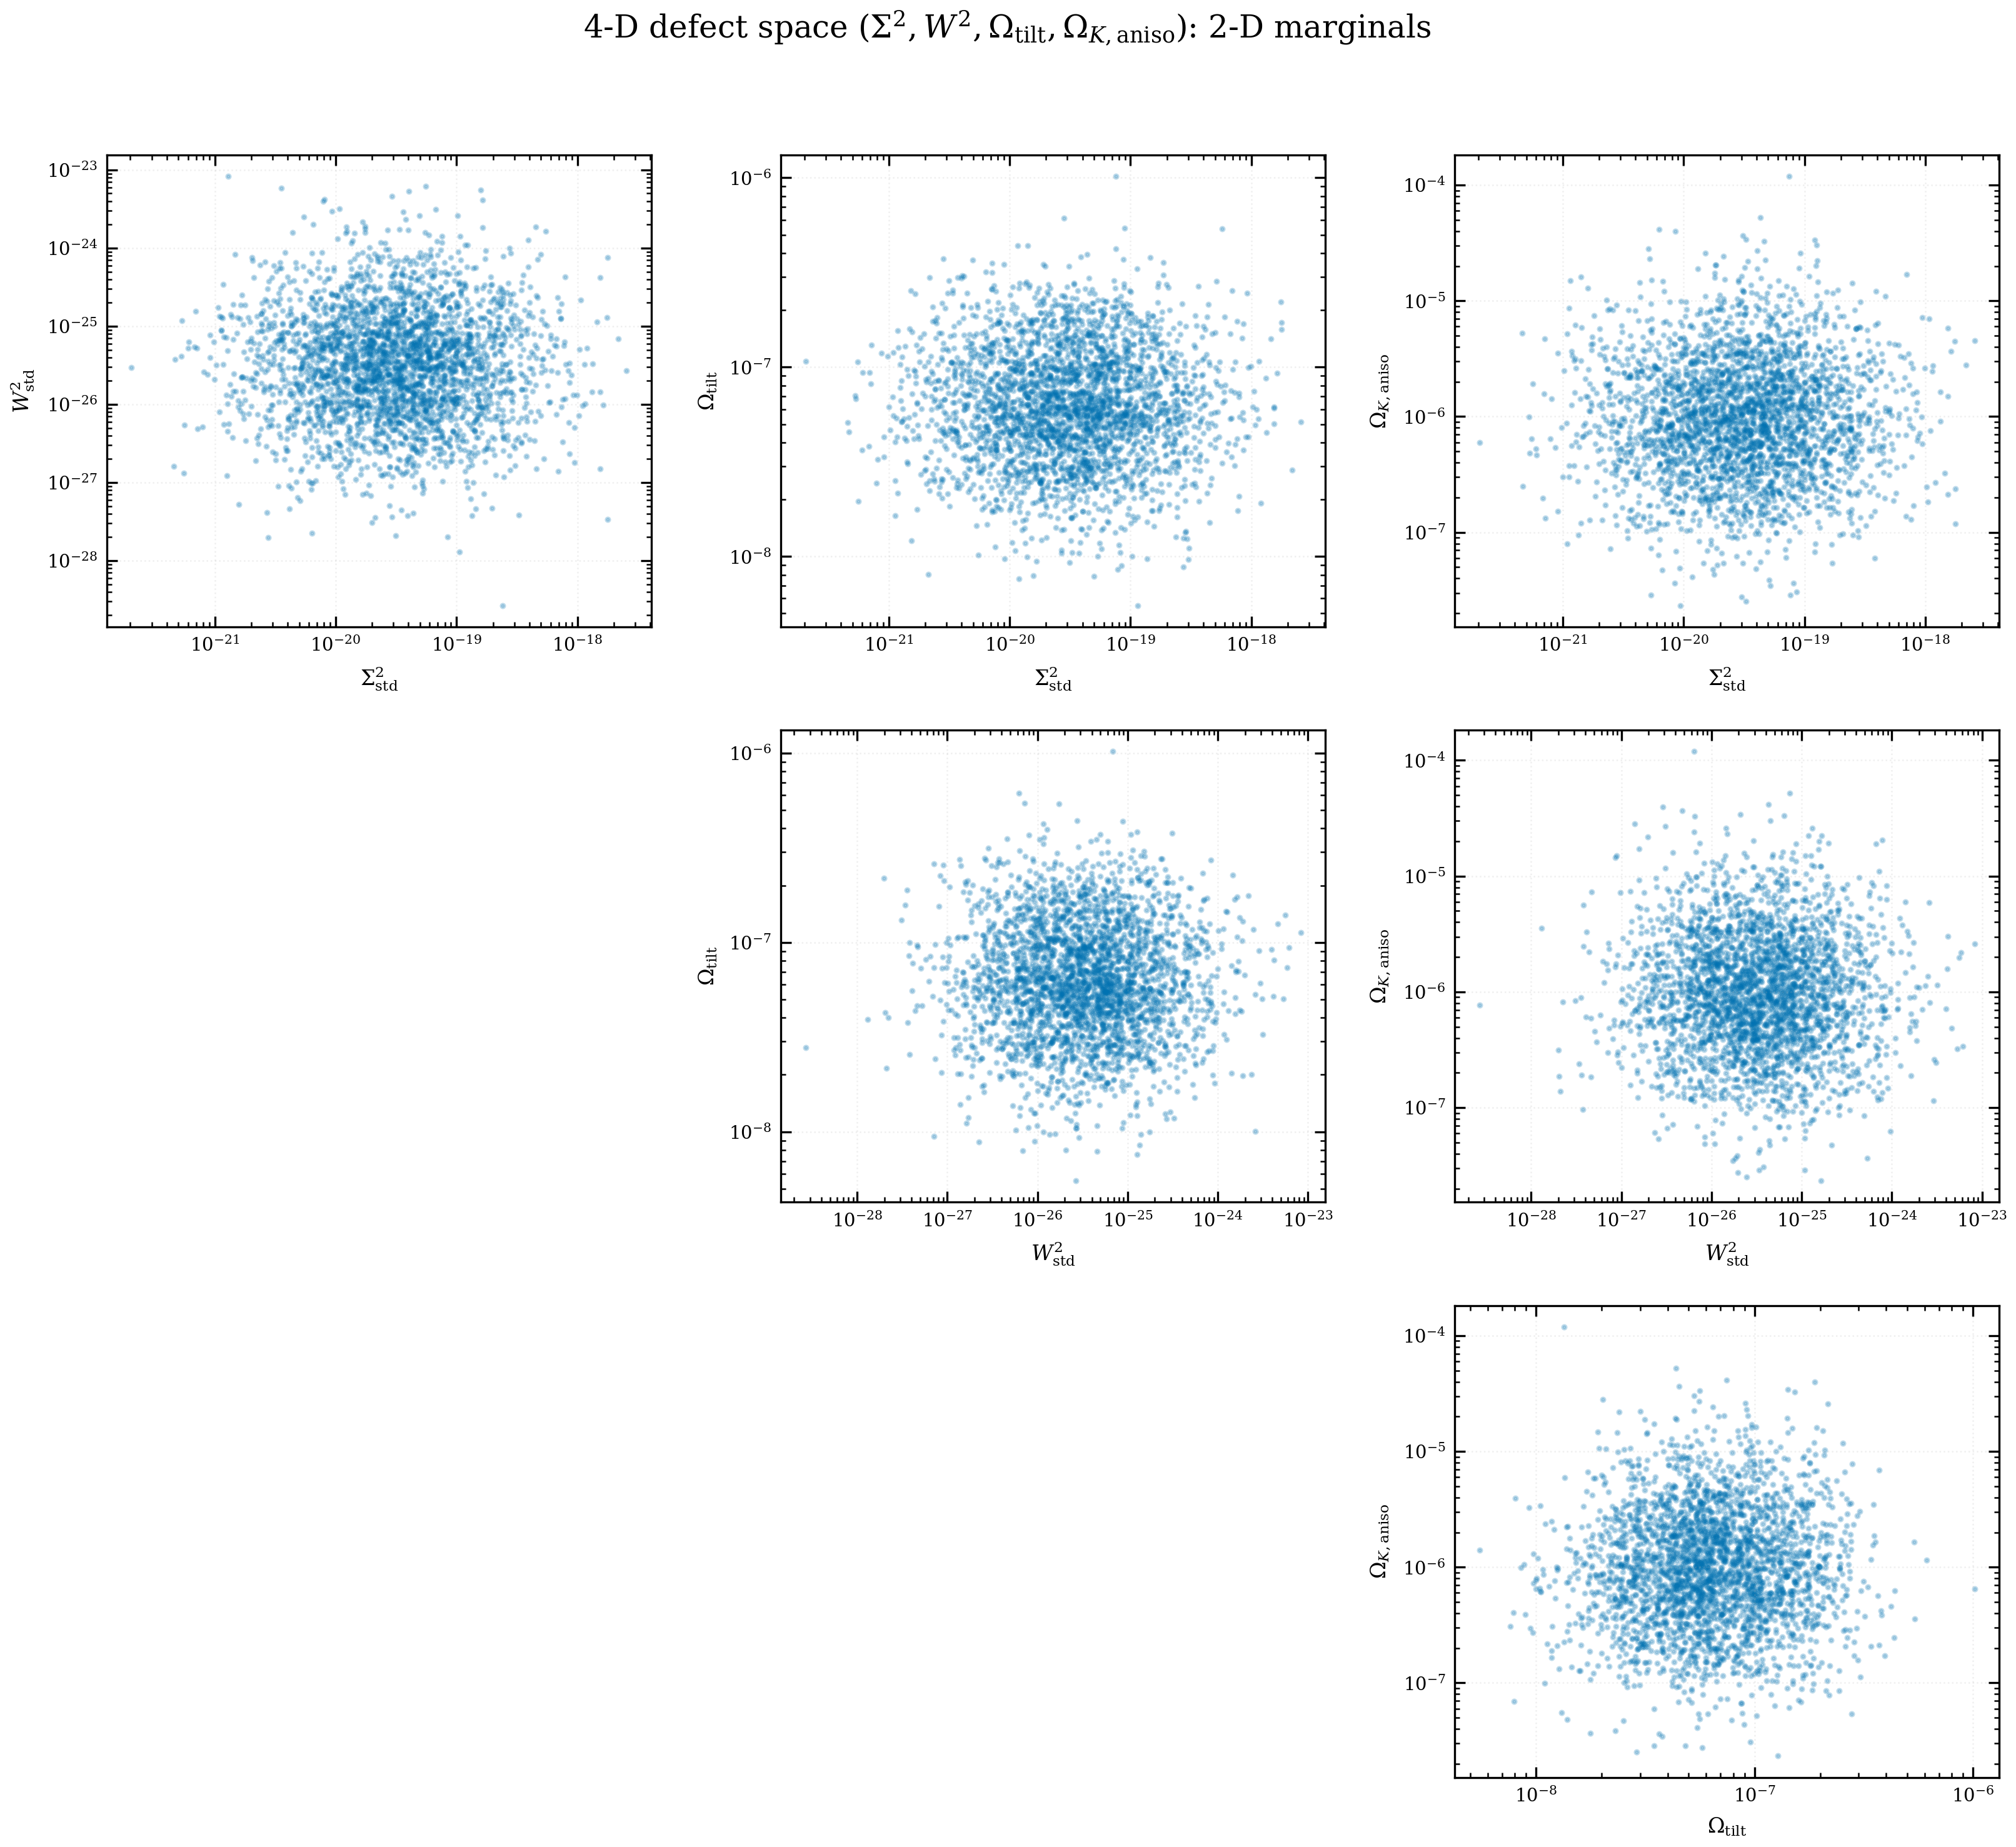
\includegraphics[width=0.82\textwidth,height=0.58\textheight,keepaspectratio]{conditioned_legacy/quarantined-legacy-root-sources__fig_4D_projection_atlas}
\captionof{figure}{Conditioned legacy diagnostic: 4D projection atlas. Condition: legacy manuscript-generator assumptions. See sidecar manifest for provenance and caveats; appendix-only, not native-transfer or family-ID evidence.}
\label{fig:conditioned-legacy-quarantined-legacy-root-sources-fig-4d-projection-atlas}
\end{center}

\clearpage
\begin{center}
\centering
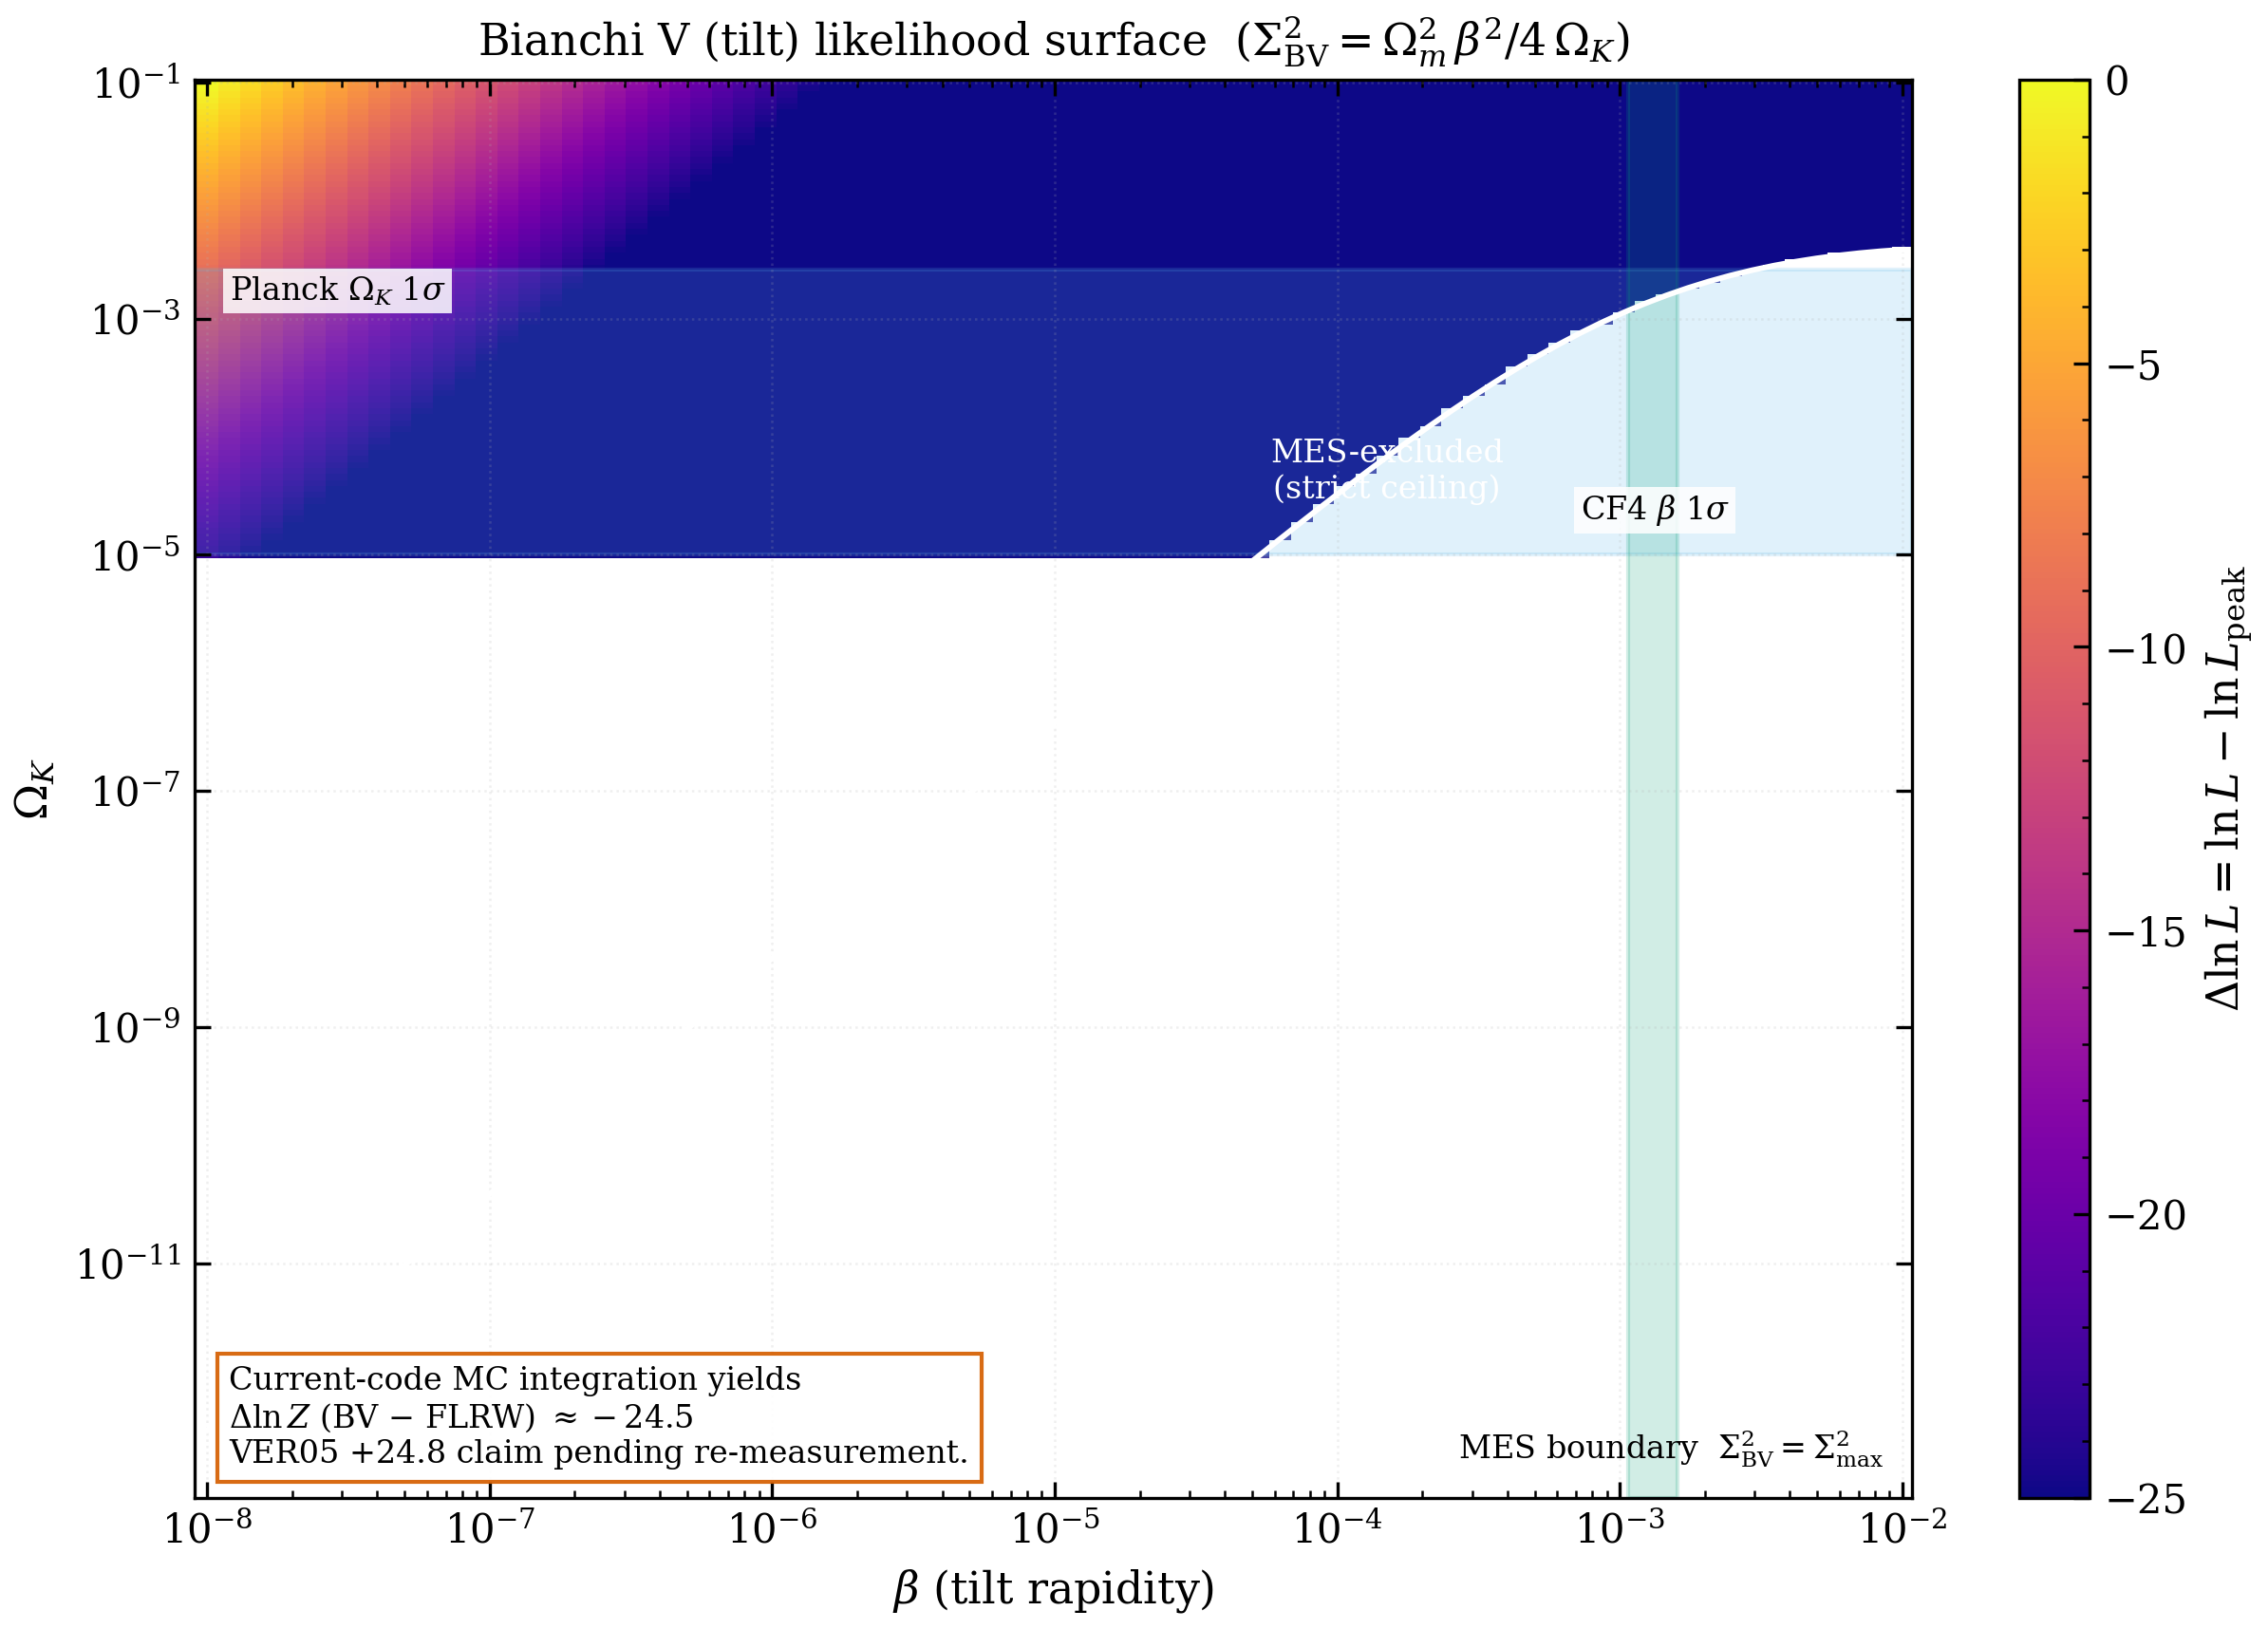
\includegraphics[width=0.82\textwidth,height=0.58\textheight,keepaspectratio]{conditioned_legacy/quarantined-legacy-root-sources__fig_BV_exclusion_restyled}
\captionof{figure}{Conditioned legacy diagnostic: BV exclusion restyled. Condition: legacy manuscript-generator assumptions. See sidecar manifest for provenance and caveats; appendix-only, not native-transfer or family-ID evidence.}
\label{fig:conditioned-legacy-quarantined-legacy-root-sources-fig-bv-exclusion-restyled}
\end{center}

\clearpage
\begin{center}
\centering
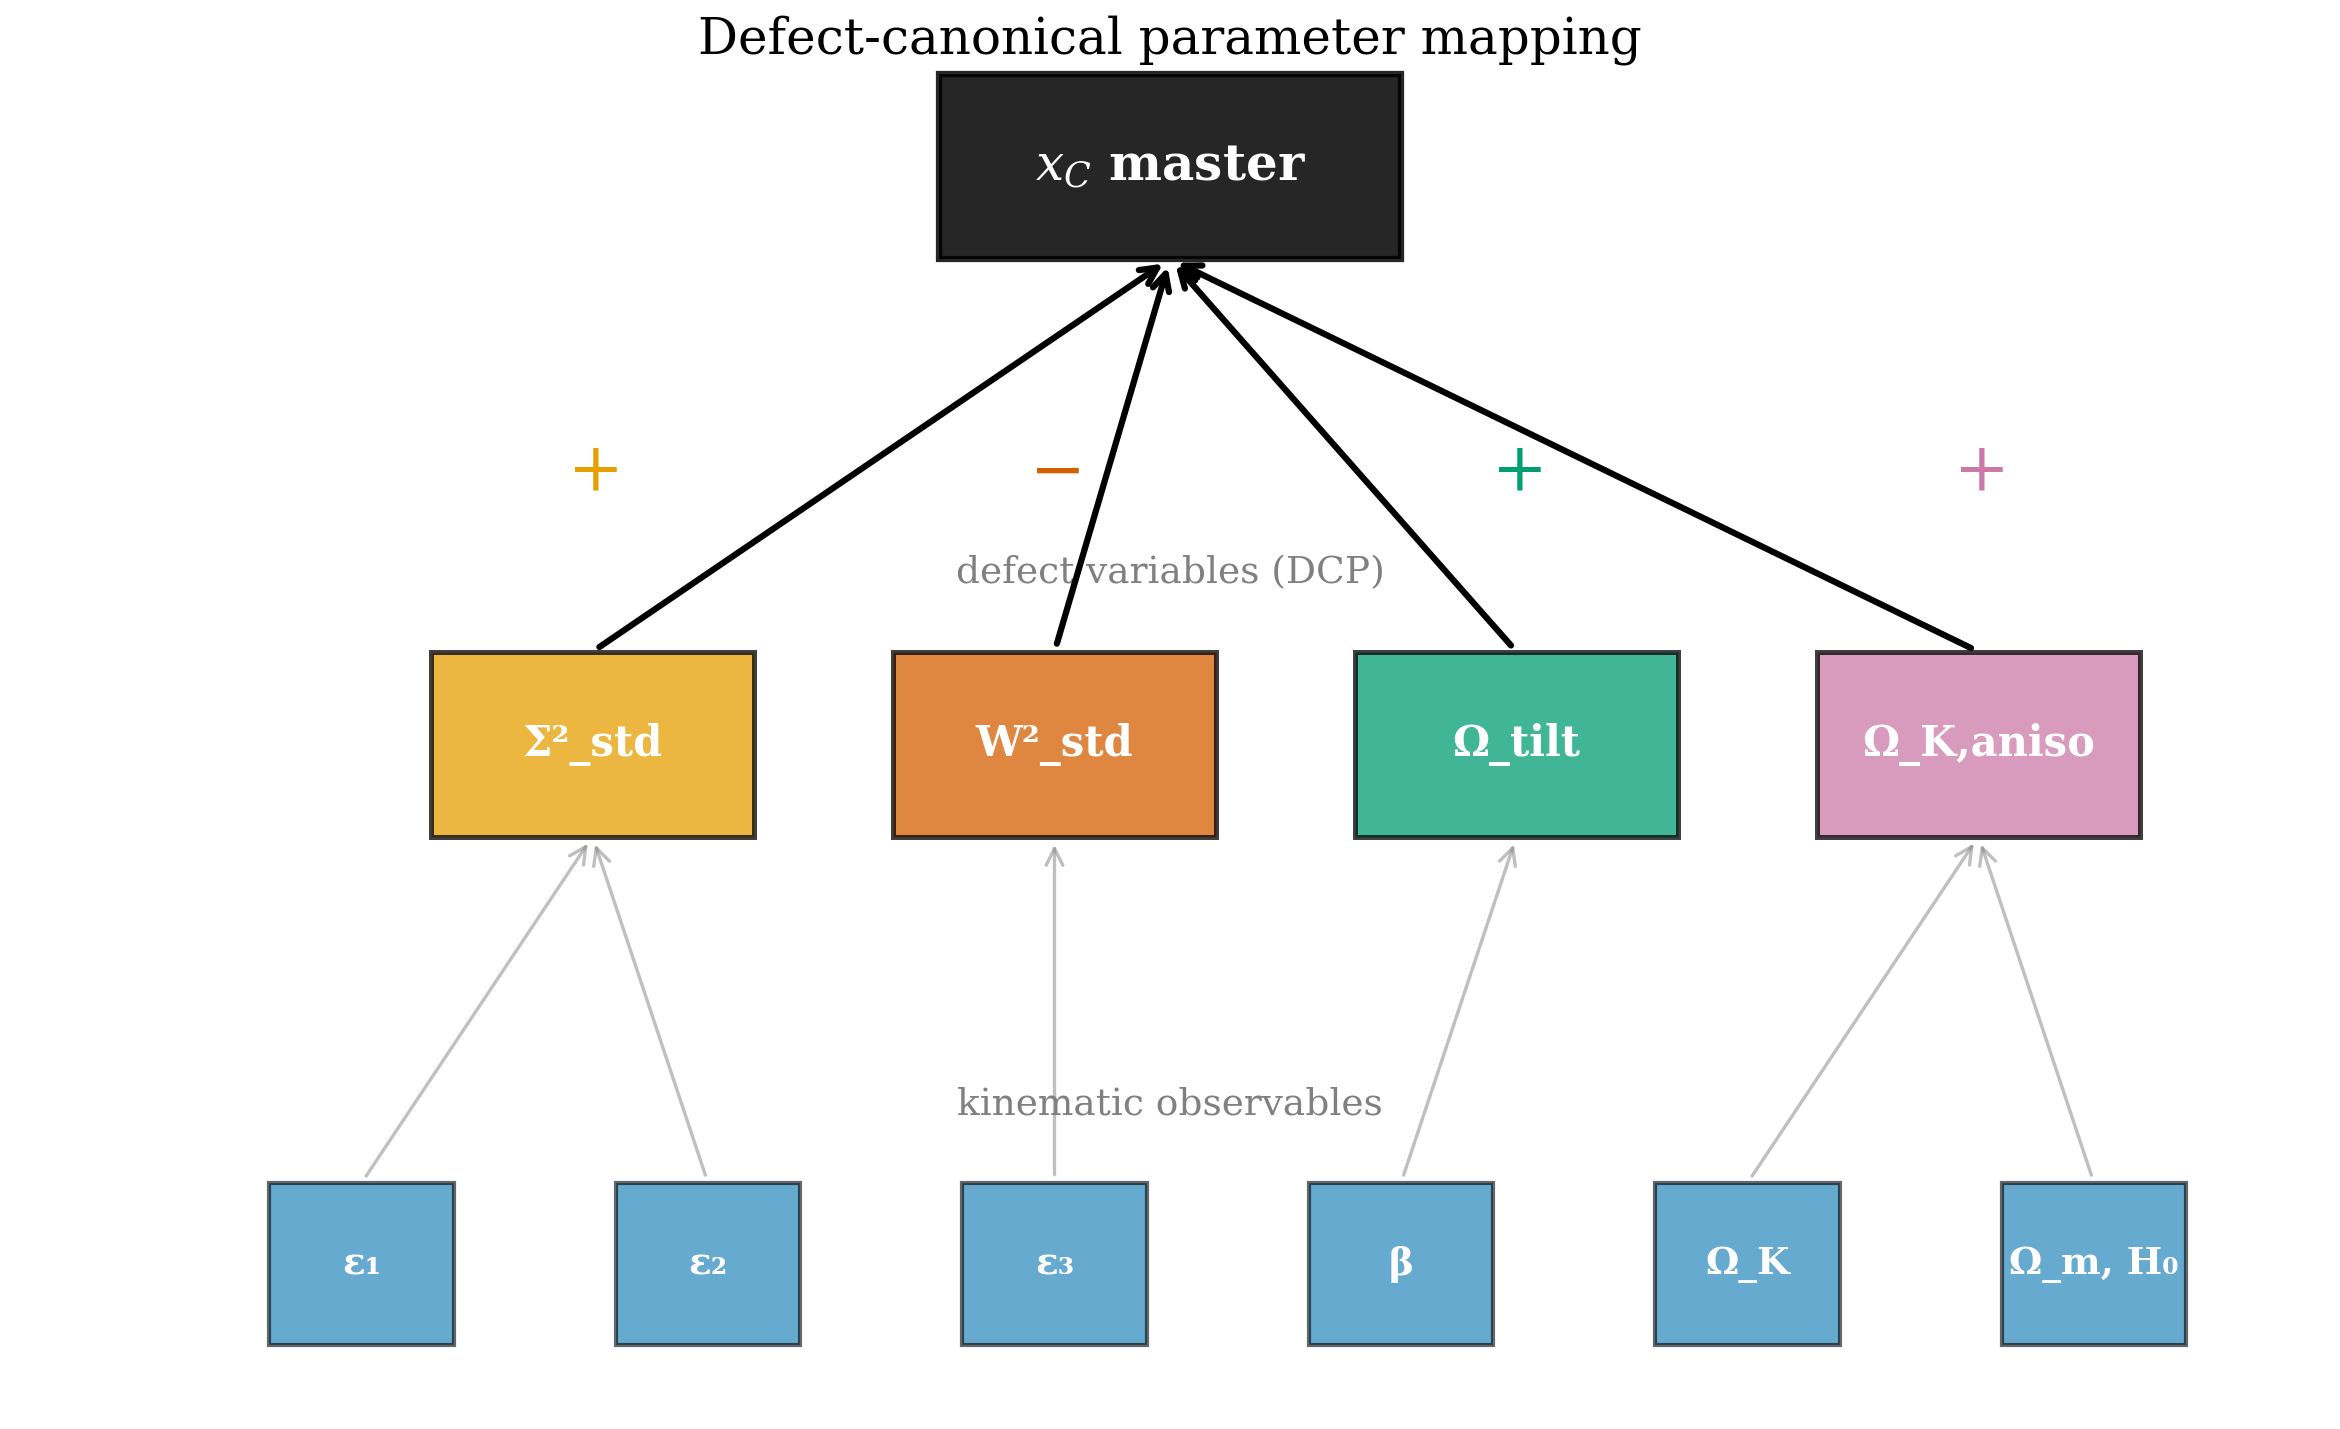
\includegraphics[width=0.82\textwidth,height=0.58\textheight,keepaspectratio]{conditioned_legacy/quarantined-legacy-root-sources__fig_DCP_defect_mapping}
\captionof{figure}{Conditioned legacy diagnostic: DCP defect mapping. Condition: legacy manuscript-generator assumptions. See sidecar manifest for provenance and caveats; appendix-only, not native-transfer or family-ID evidence.}
\label{fig:conditioned-legacy-quarantined-legacy-root-sources-fig-dcp-defect-mapping}
\end{center}

\clearpage
\begin{center}
\centering
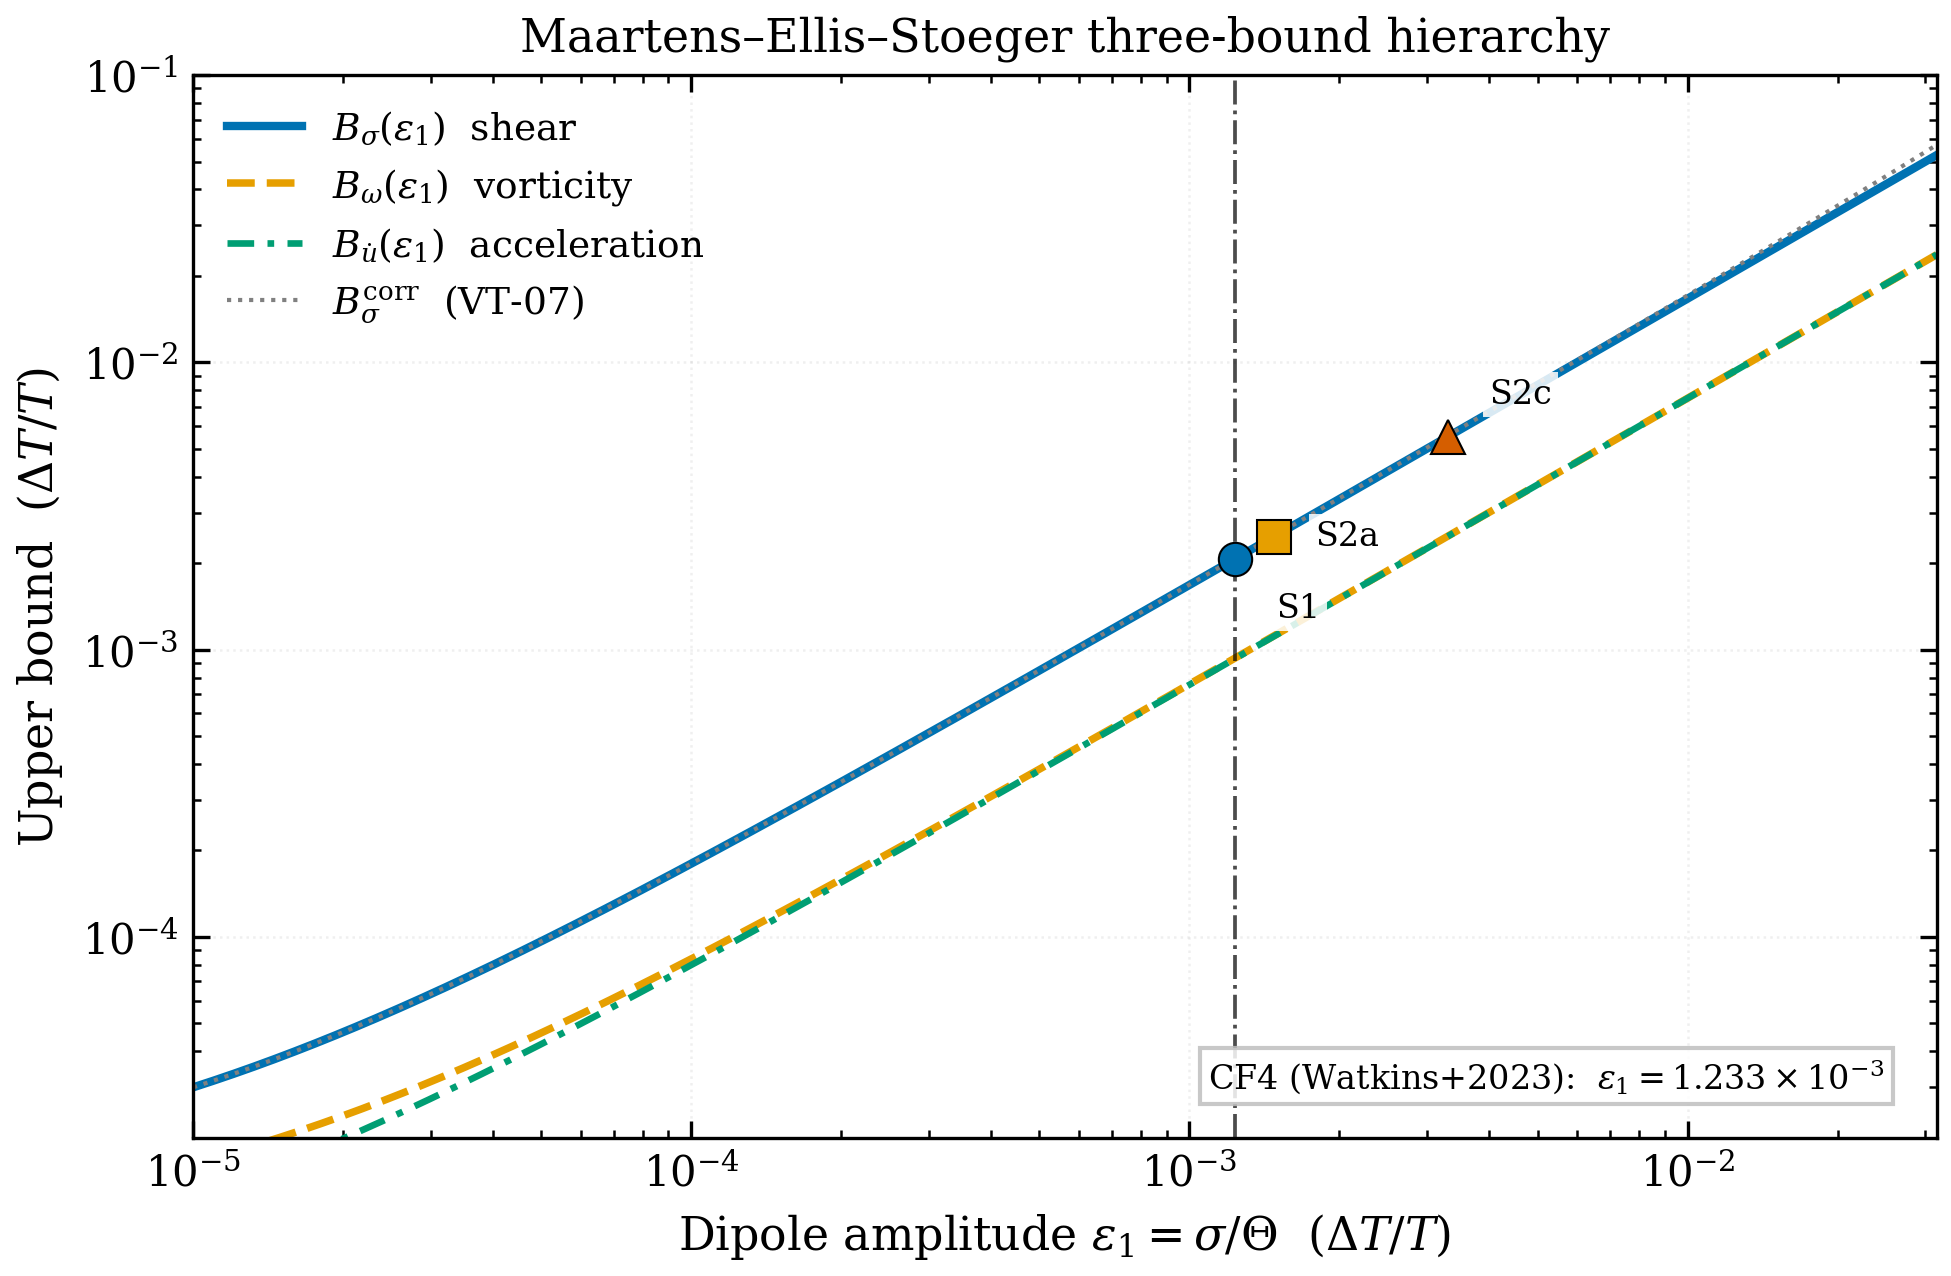
\includegraphics[width=0.82\textwidth,height=0.58\textheight,keepaspectratio]{conditioned_legacy/quarantined-legacy-root-sources__fig_MES_three_bounds}
\captionof{figure}{Conditioned legacy diagnostic: MES three bounds. Condition: legacy manuscript-generator assumptions. See sidecar manifest for provenance and caveats; appendix-only, not native-transfer or family-ID evidence.}
\label{fig:conditioned-legacy-quarantined-legacy-root-sources-fig-mes-three-bounds}
\end{center}

\clearpage
\begin{center}
\centering
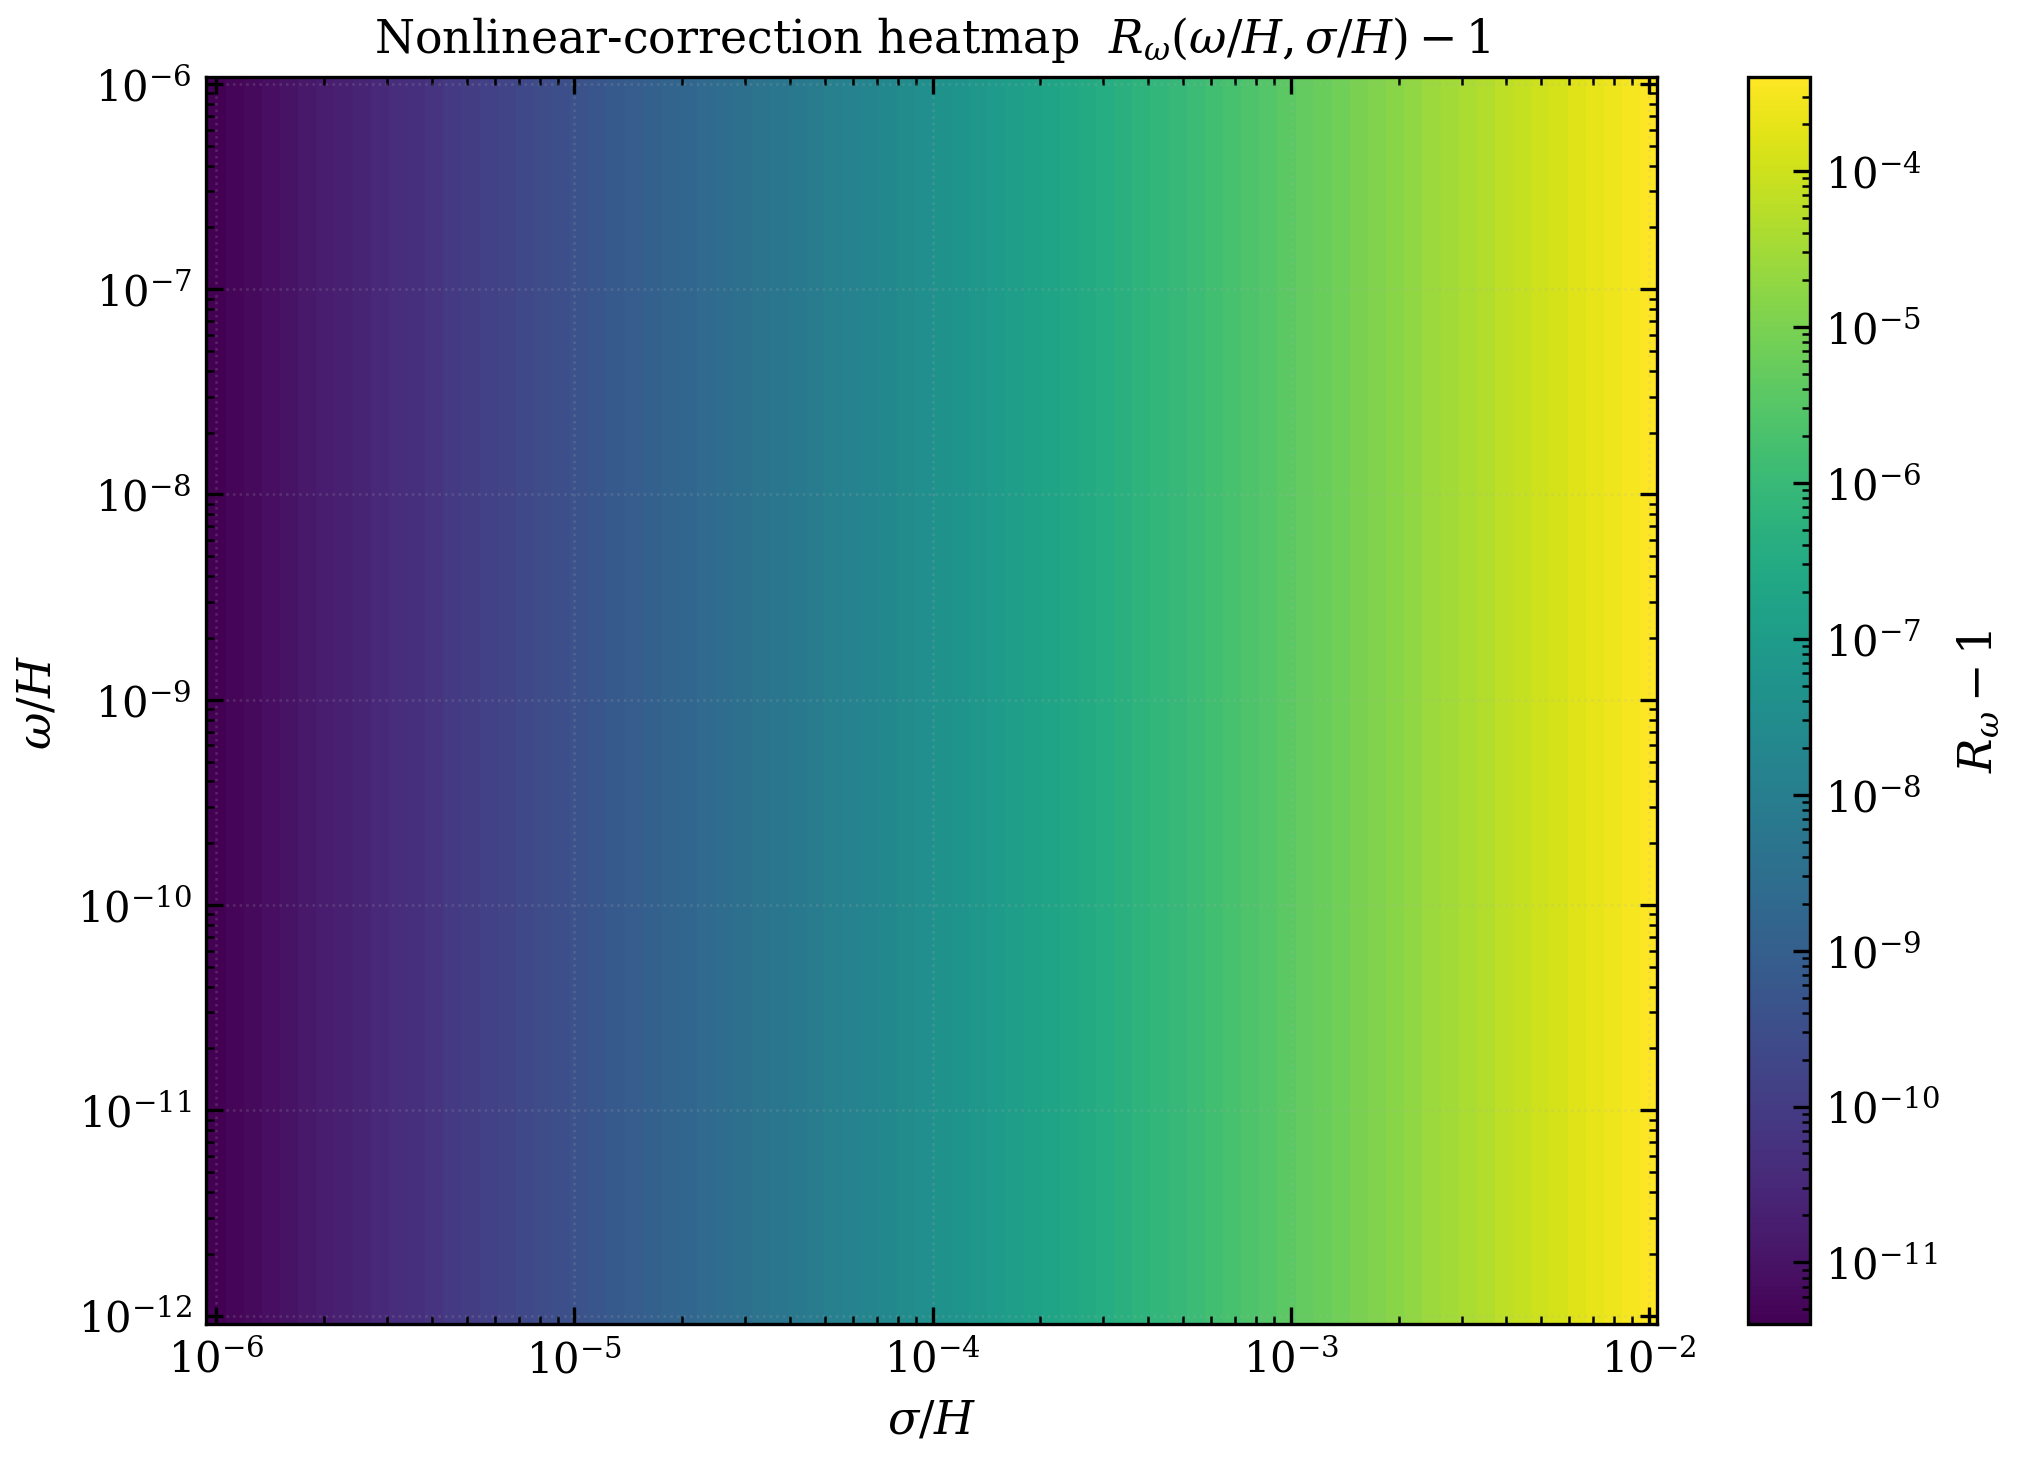
\includegraphics[width=0.82\textwidth,height=0.58\textheight,keepaspectratio]{conditioned_legacy/quarantined-legacy-root-sources__fig_NL_heatmap}
\captionof{figure}{Conditioned legacy diagnostic: NL heatmap. Condition: legacy manuscript-generator assumptions. See sidecar manifest for provenance and caveats; appendix-only, not native-transfer or family-ID evidence.}
\label{fig:conditioned-legacy-quarantined-legacy-root-sources-fig-nl-heatmap}
\end{center}

\clearpage
\begin{center}
\centering
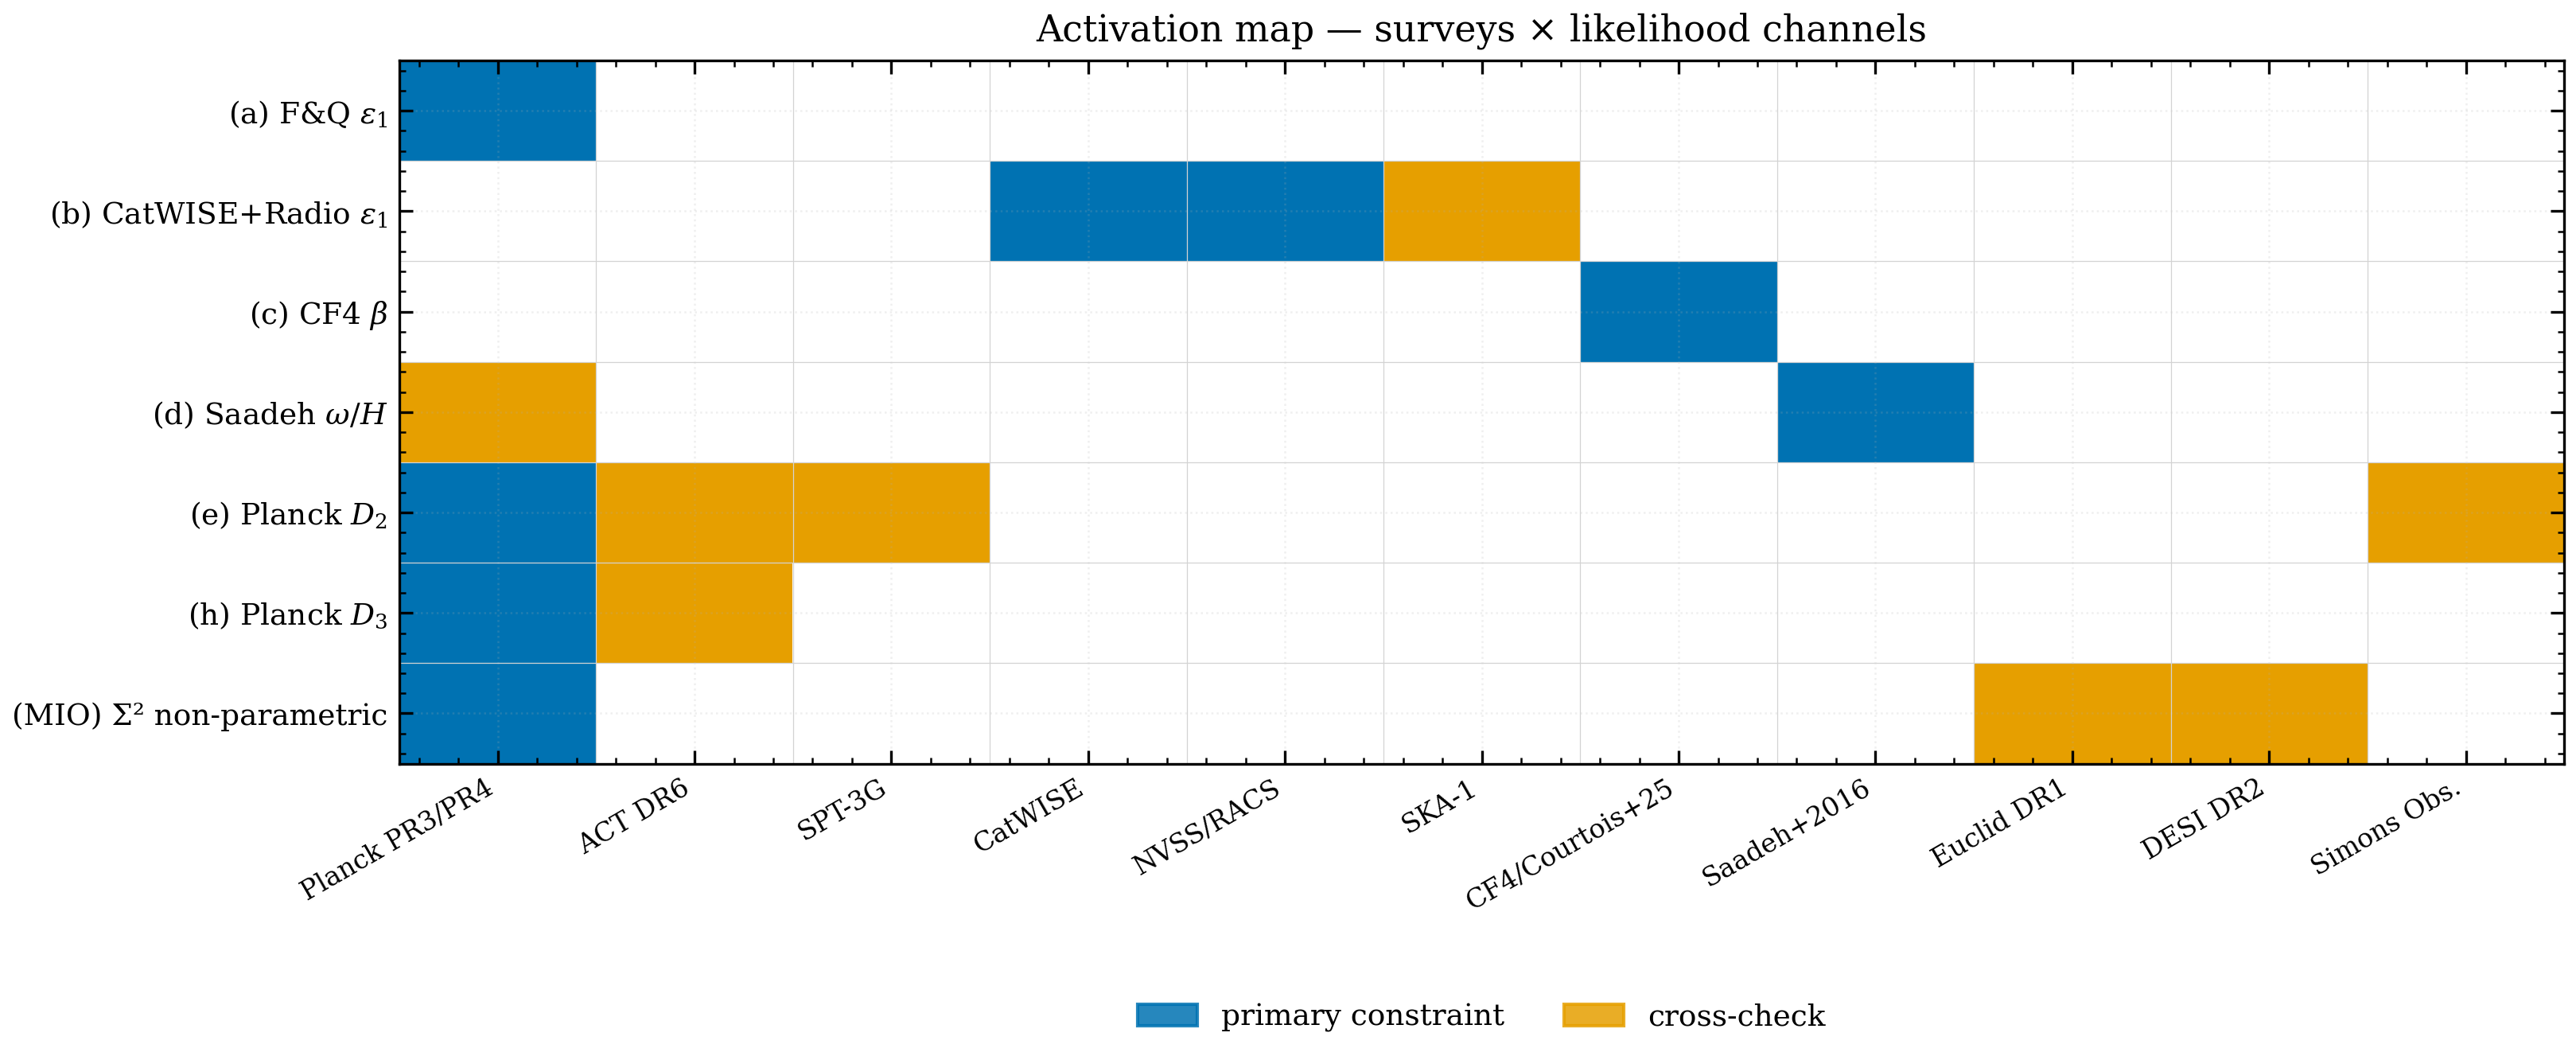
\includegraphics[width=0.82\textwidth,height=0.58\textheight,keepaspectratio]{conditioned_legacy/quarantined-legacy-root-sources__fig_activation_map}
\captionof{figure}{Conditioned legacy diagnostic: activation map. Condition: legacy manuscript-generator assumptions. See sidecar manifest for provenance and caveats; appendix-only, not native-transfer or family-ID evidence.}
\label{fig:conditioned-legacy-quarantined-legacy-root-sources-fig-activation-map}
\end{center}

\clearpage
\begin{center}
\centering
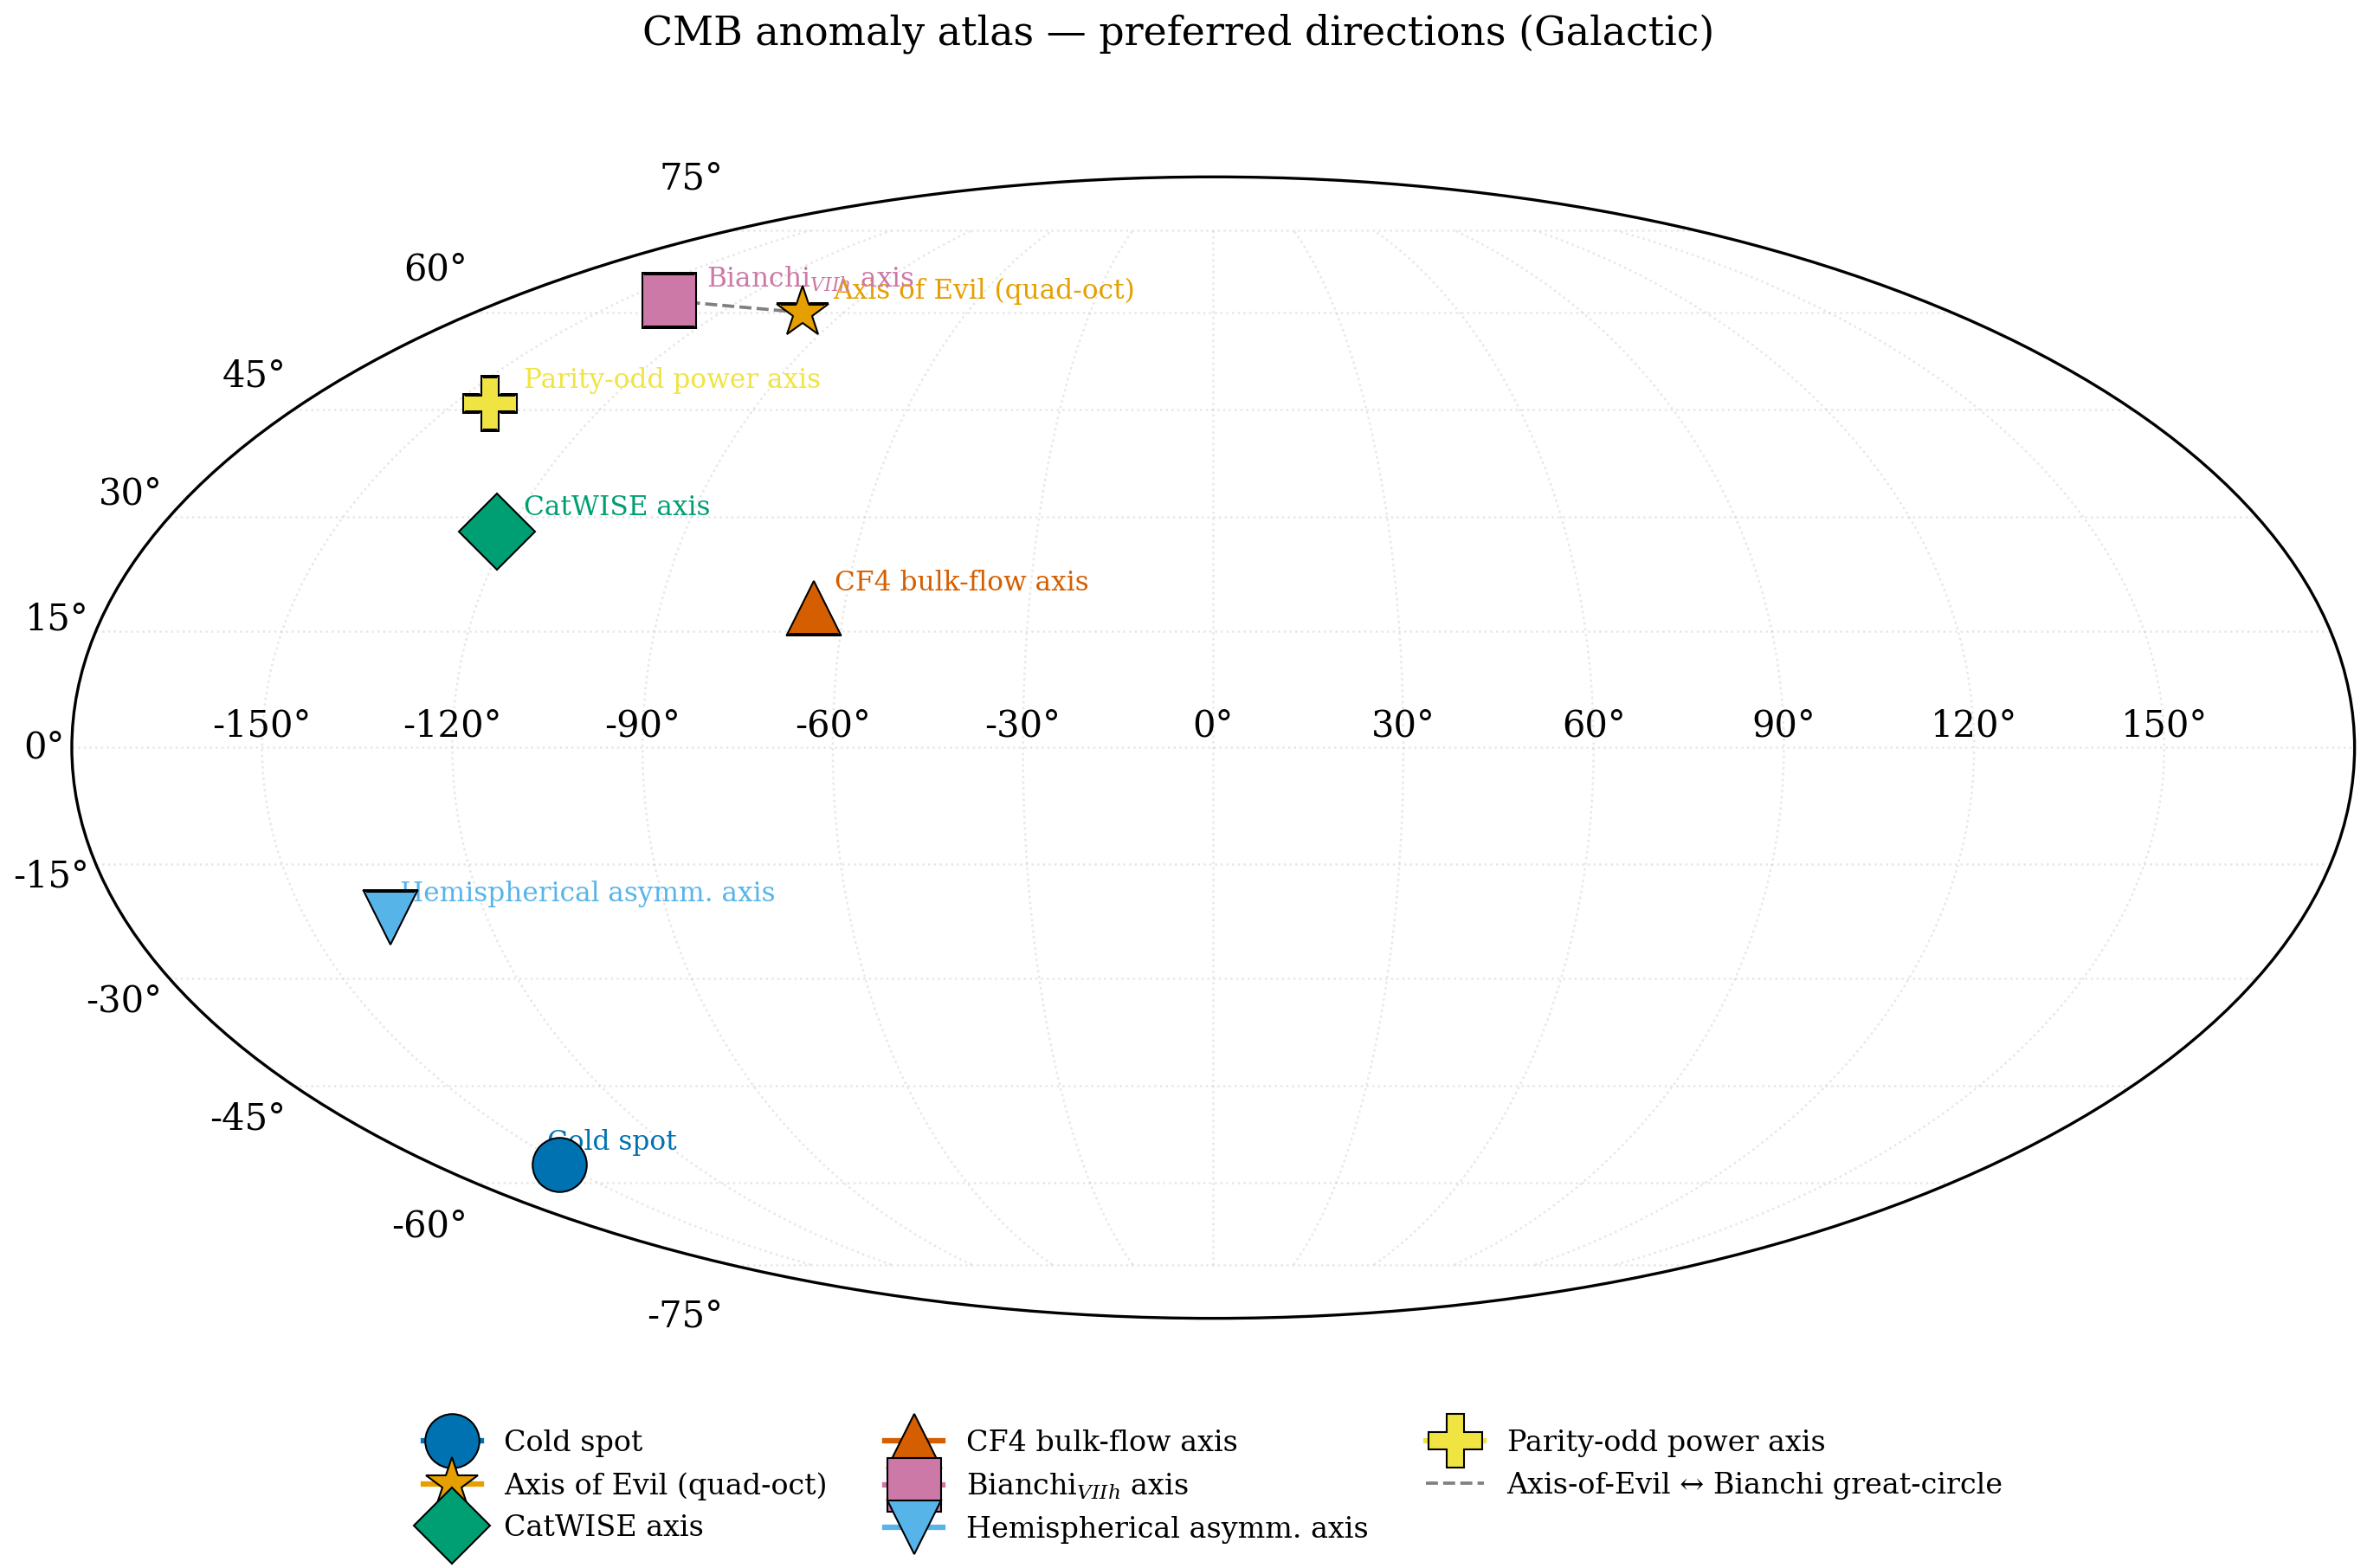
\includegraphics[width=0.82\textwidth,height=0.58\textheight,keepaspectratio]{conditioned_legacy/quarantined-legacy-root-sources__fig_anomaly_atlas_skymap}
\captionof{figure}{Conditioned legacy diagnostic: anomaly atlas skymap. Condition: directional artifact with current sky/mask support unresolved. See sidecar manifest for provenance and caveats; appendix-only, not native-transfer or family-ID evidence.}
\label{fig:conditioned-legacy-quarantined-legacy-root-sources-fig-anomaly-atlas-skymap}
\end{center}

\clearpage
\begin{center}
\centering
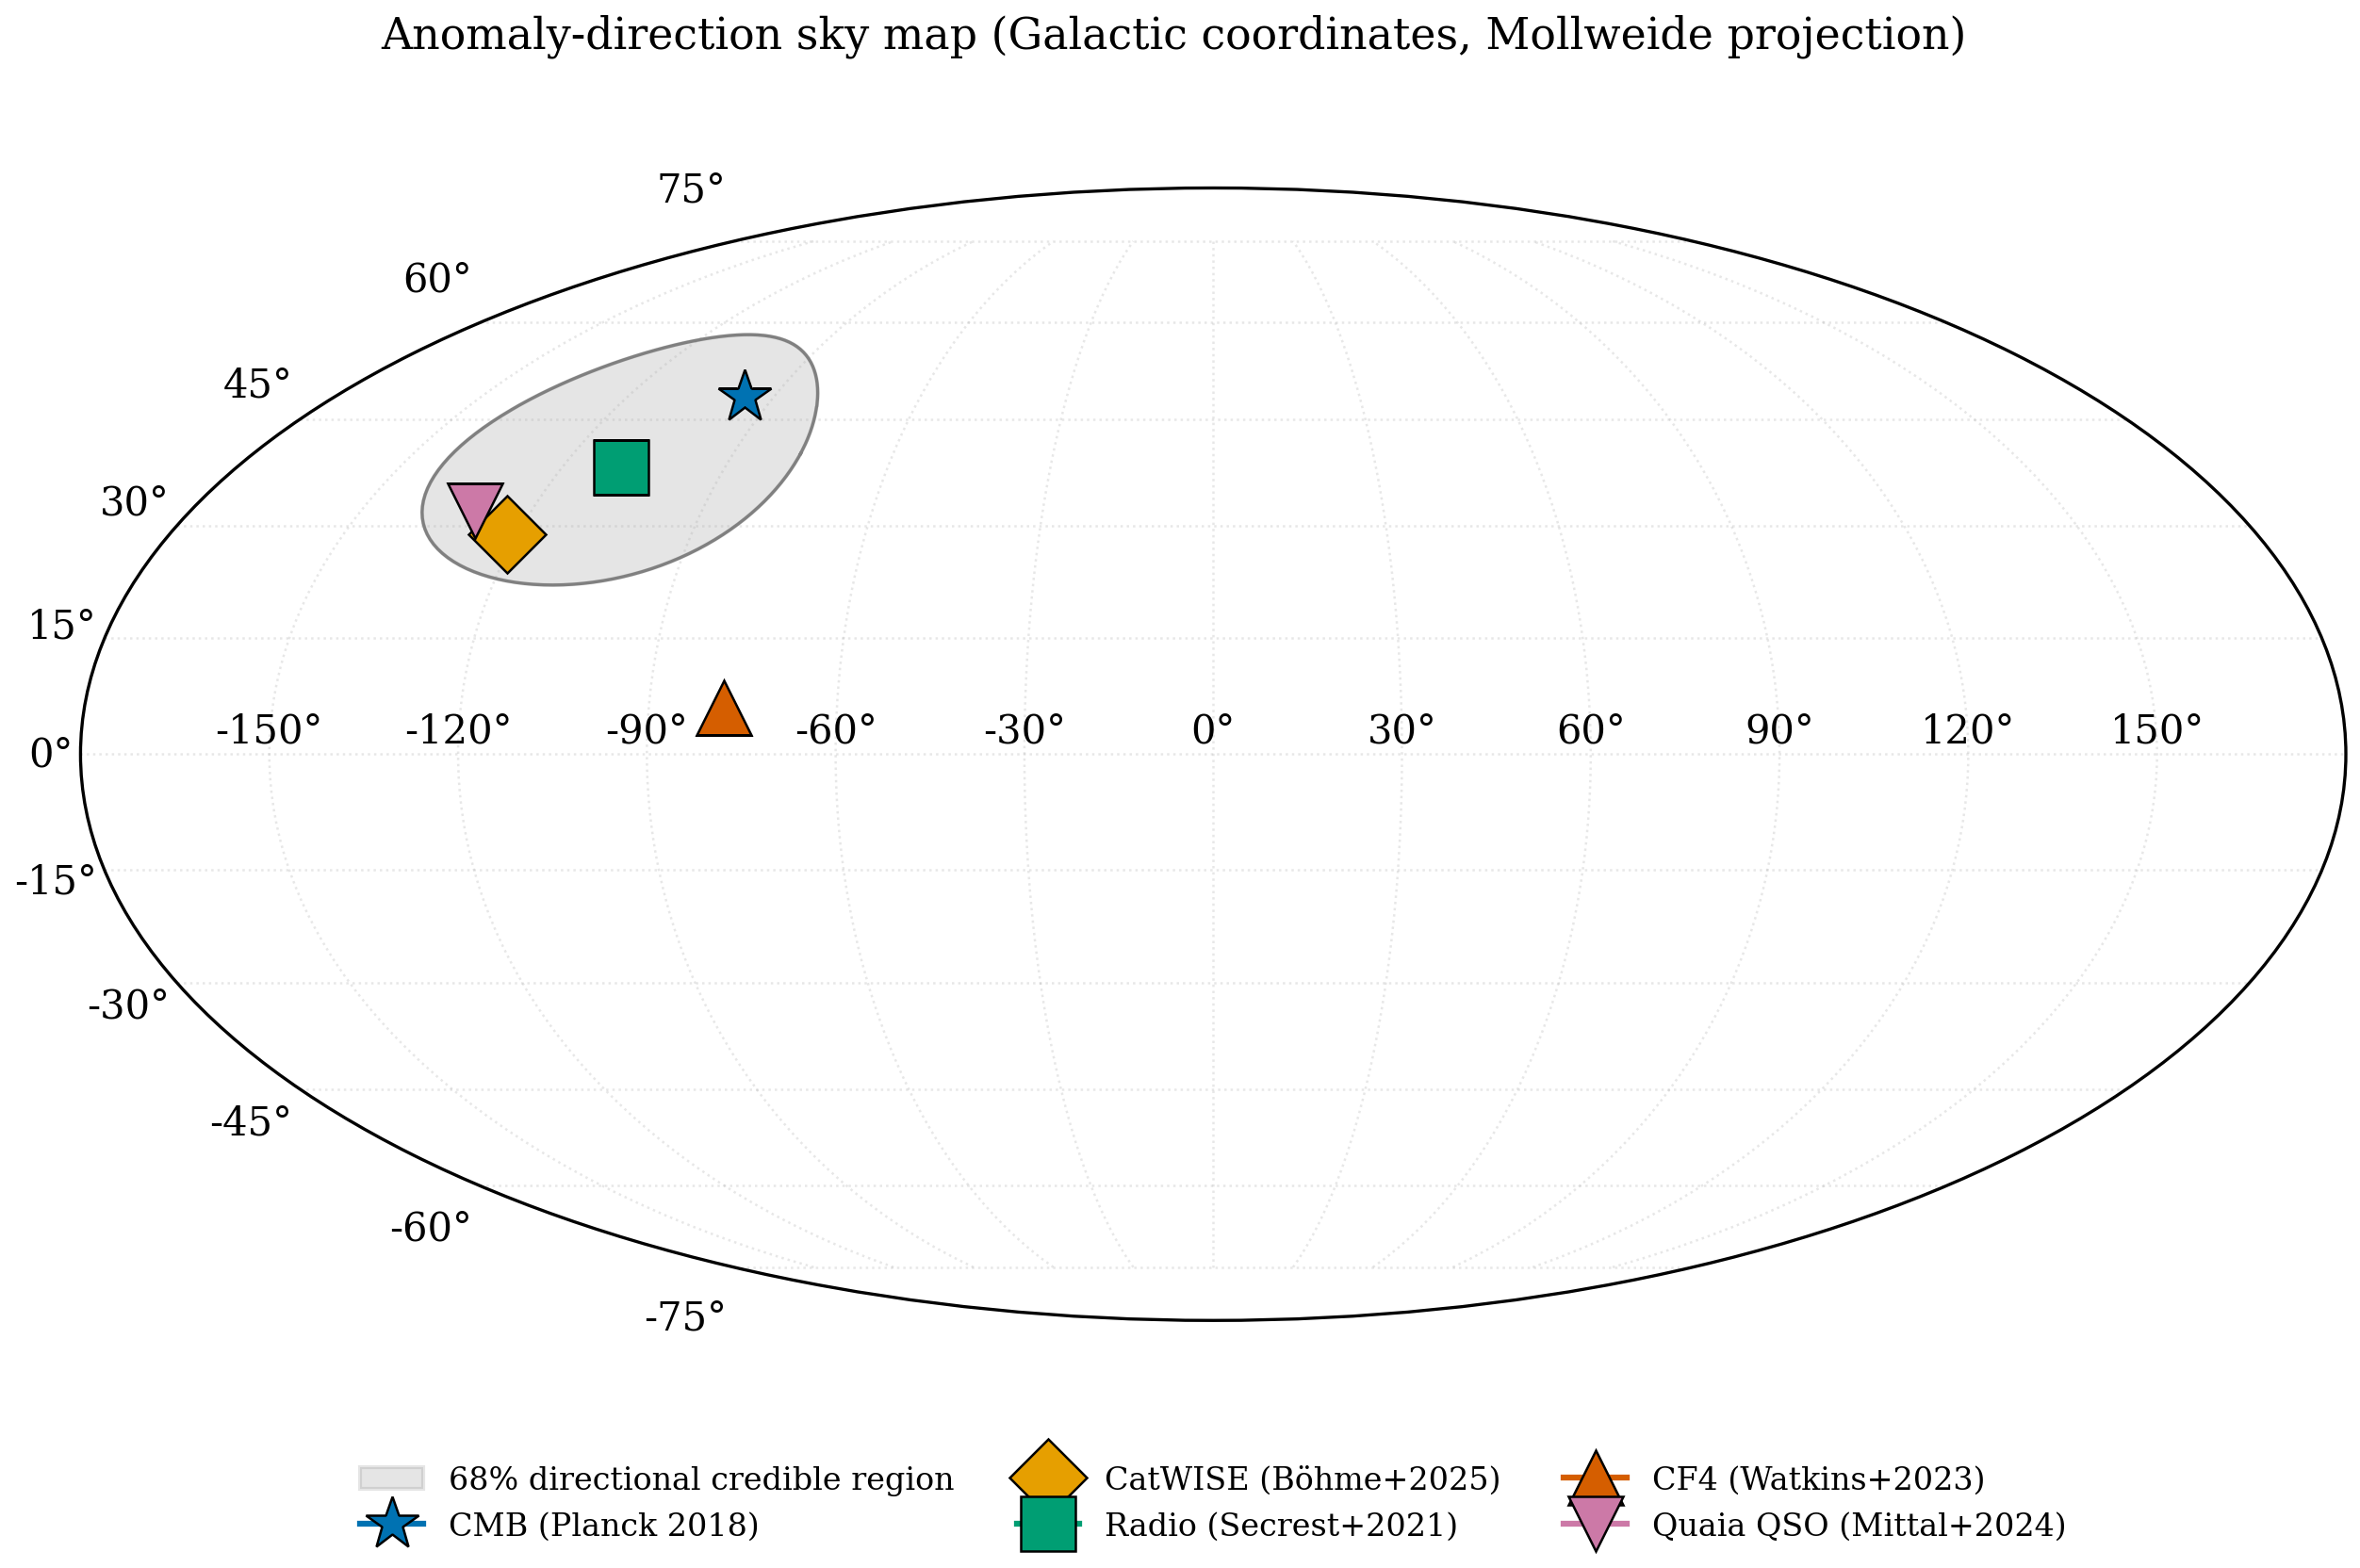
\includegraphics[width=0.82\textwidth,height=0.58\textheight,keepaspectratio]{conditioned_legacy/quarantined-legacy-root-sources__fig_anomaly_direction_sky}
\captionof{figure}{Conditioned legacy diagnostic: anomaly direction sky. Condition: directional artifact with current sky/mask support unresolved. See sidecar manifest for provenance and caveats; appendix-only, not native-transfer or family-ID evidence.}
\label{fig:conditioned-legacy-quarantined-legacy-root-sources-fig-anomaly-direction-sky}
\end{center}

\clearpage
\begin{center}
\centering
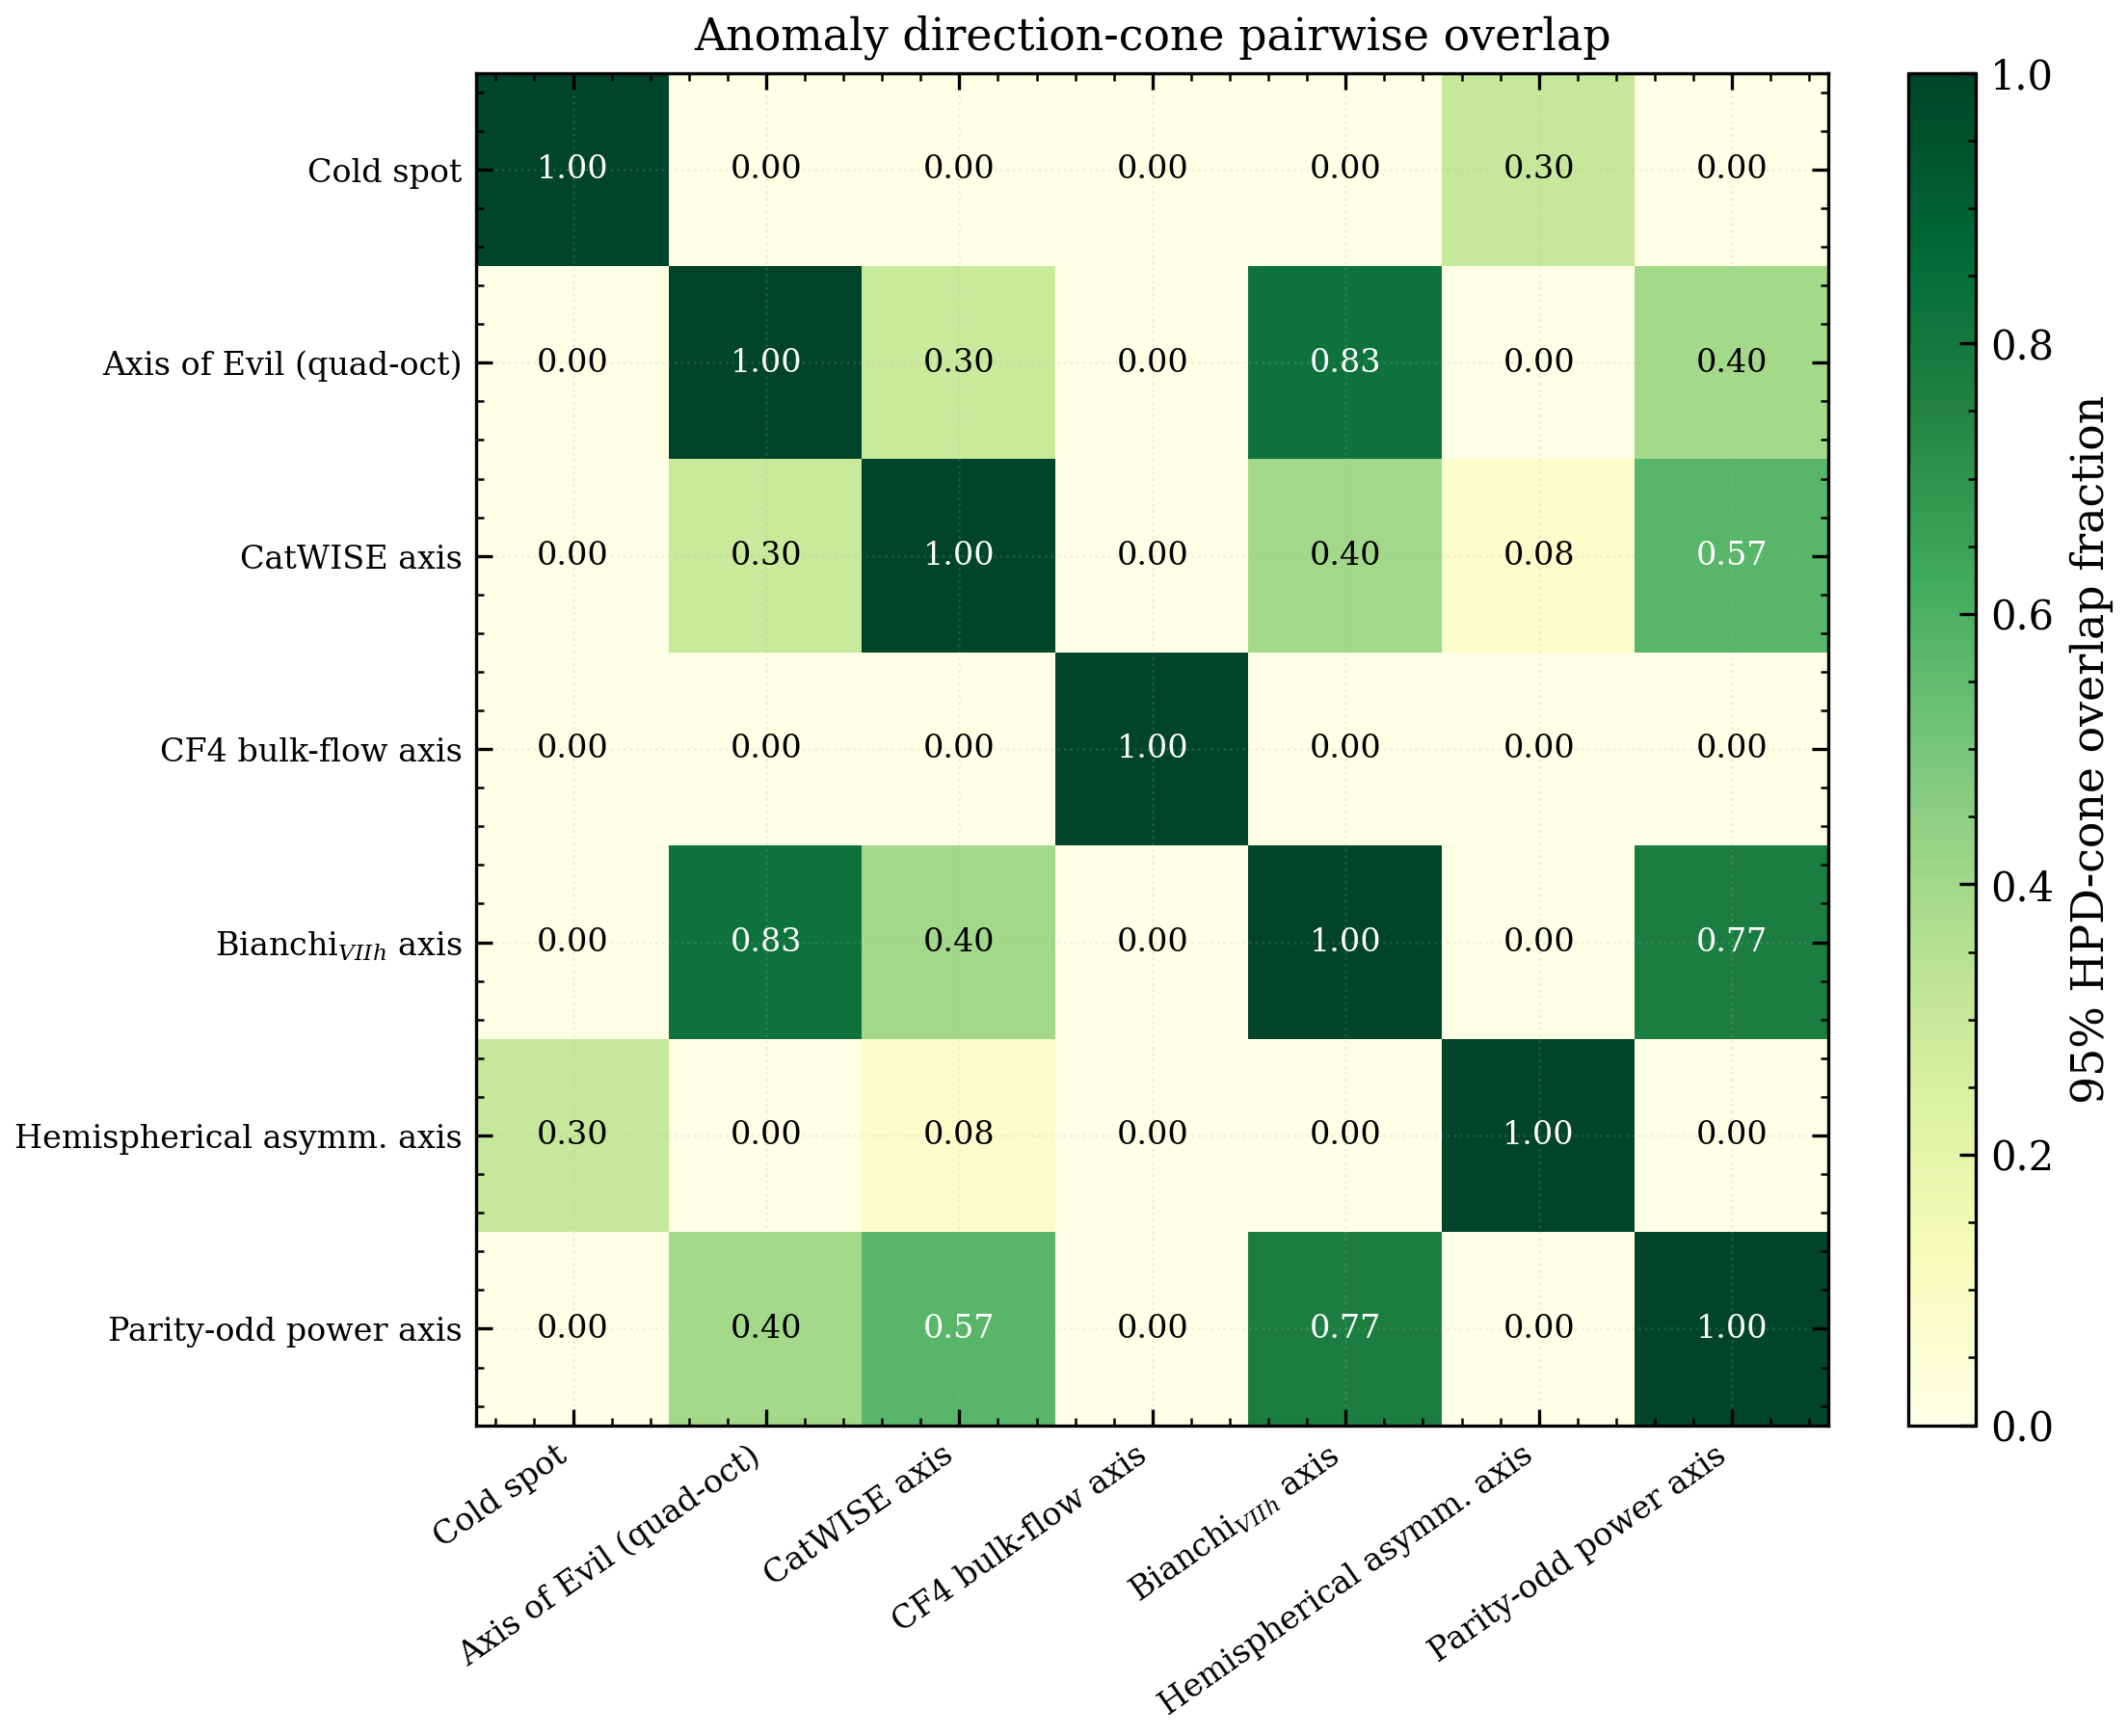
\includegraphics[width=0.82\textwidth,height=0.58\textheight,keepaspectratio]{conditioned_legacy/quarantined-legacy-root-sources__fig_anomaly_overlap_matrix}
\captionof{figure}{Conditioned legacy diagnostic: anomaly overlap matrix. Condition: legacy manuscript-generator assumptions. See sidecar manifest for provenance and caveats; appendix-only, not native-transfer or family-ID evidence.}
\label{fig:conditioned-legacy-quarantined-legacy-root-sources-fig-anomaly-overlap-matrix}
\end{center}

\clearpage
\begin{center}
\centering
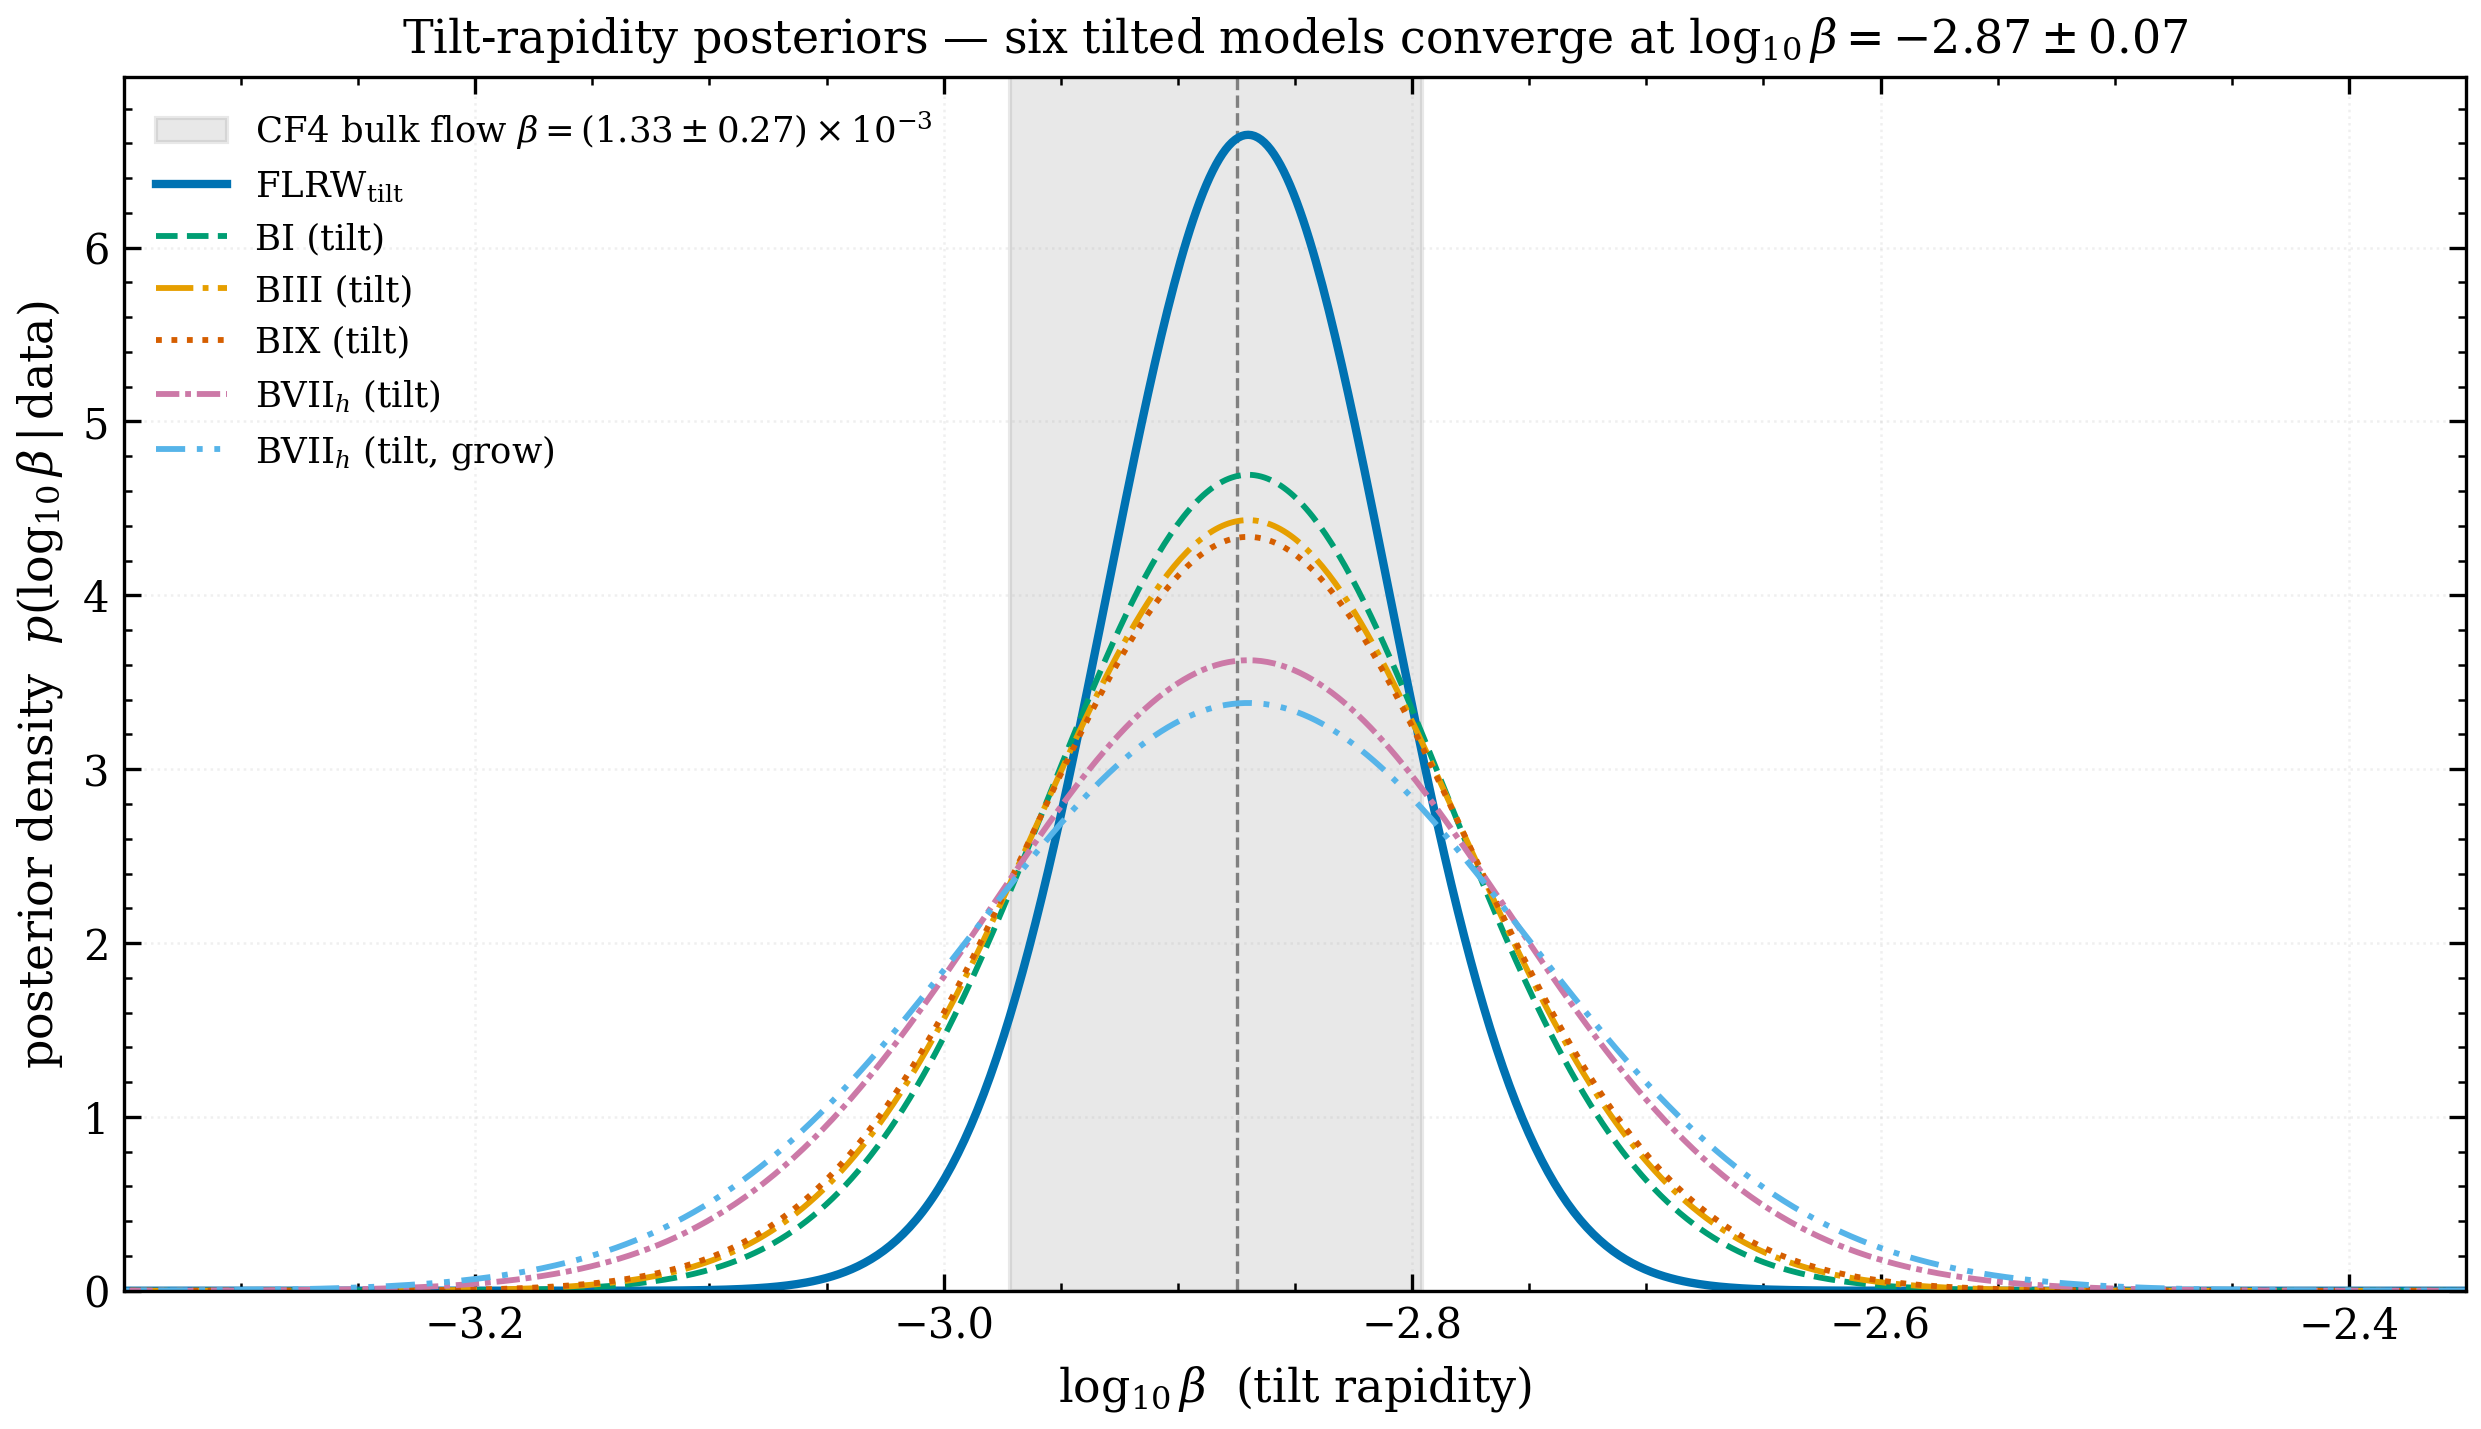
\includegraphics[width=0.82\textwidth,height=0.58\textheight,keepaspectratio]{conditioned_legacy/quarantined-legacy-root-sources__fig_beta_posteriors_R03}
\captionof{figure}{Conditioned legacy diagnostic: beta posteriors R03. Condition: legacy statistical assumptions without current null/PPC/LOOCV refresh. See sidecar manifest for provenance and caveats; appendix-only, not native-transfer or family-ID evidence.}
\label{fig:conditioned-legacy-quarantined-legacy-root-sources-fig-beta-posteriors-r03}
\end{center}

\clearpage
\begin{center}
\centering
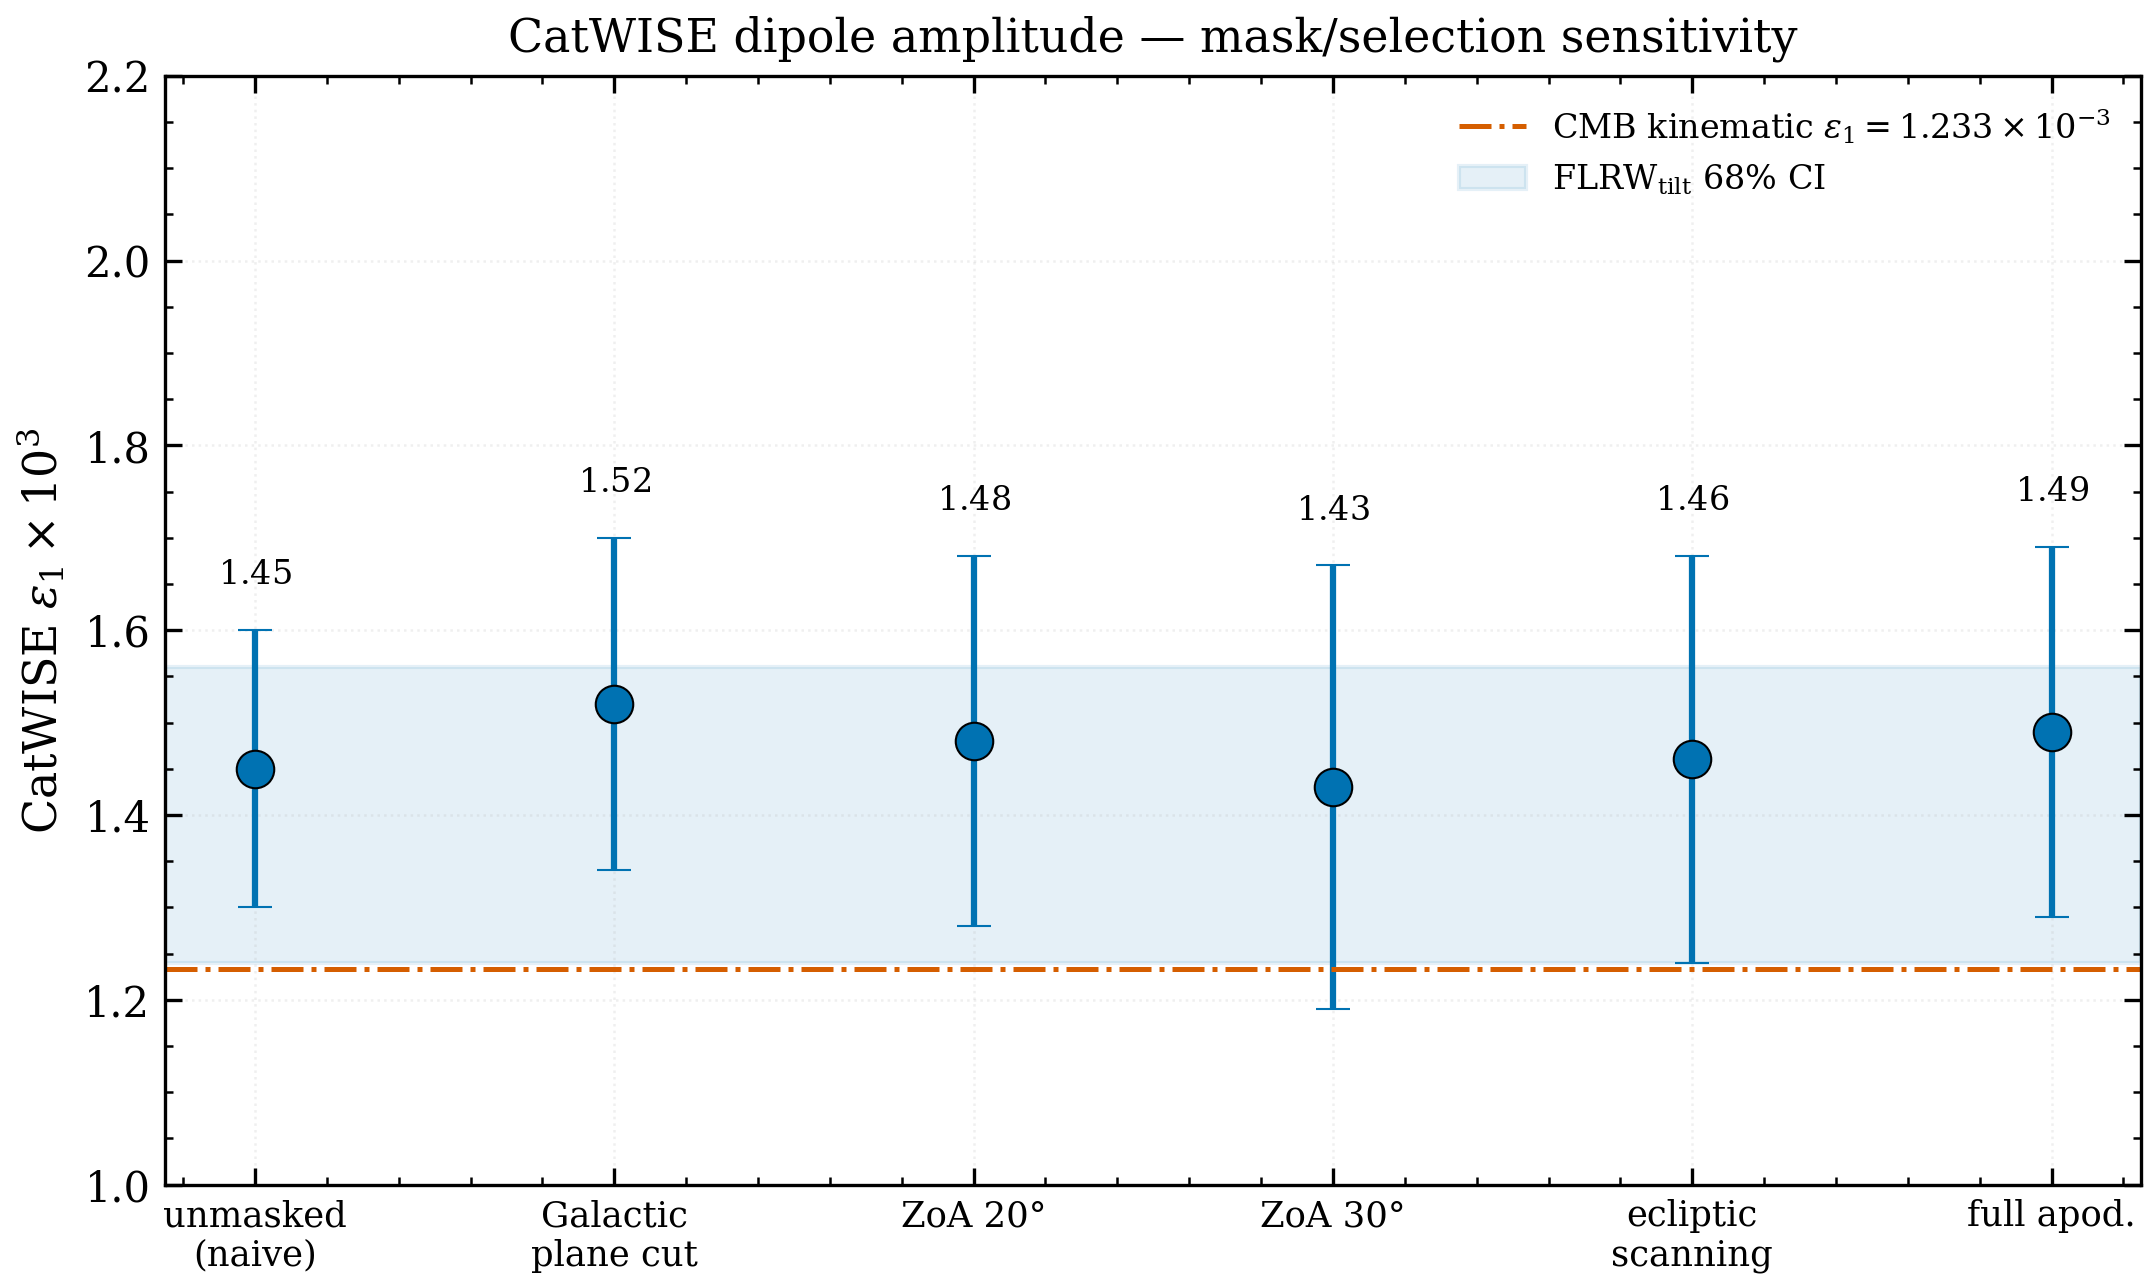
\includegraphics[width=0.82\textwidth,height=0.58\textheight,keepaspectratio]{conditioned_legacy/quarantined-legacy-root-sources__fig_catwise_sensitivity}
\captionof{figure}{Conditioned legacy diagnostic: catwise sensitivity. Condition: legacy manuscript-generator assumptions. See sidecar manifest for provenance and caveats; appendix-only, not native-transfer or family-ID evidence.}
\label{fig:conditioned-legacy-quarantined-legacy-root-sources-fig-catwise-sensitivity}
\end{center}

\clearpage
\begin{center}
\centering
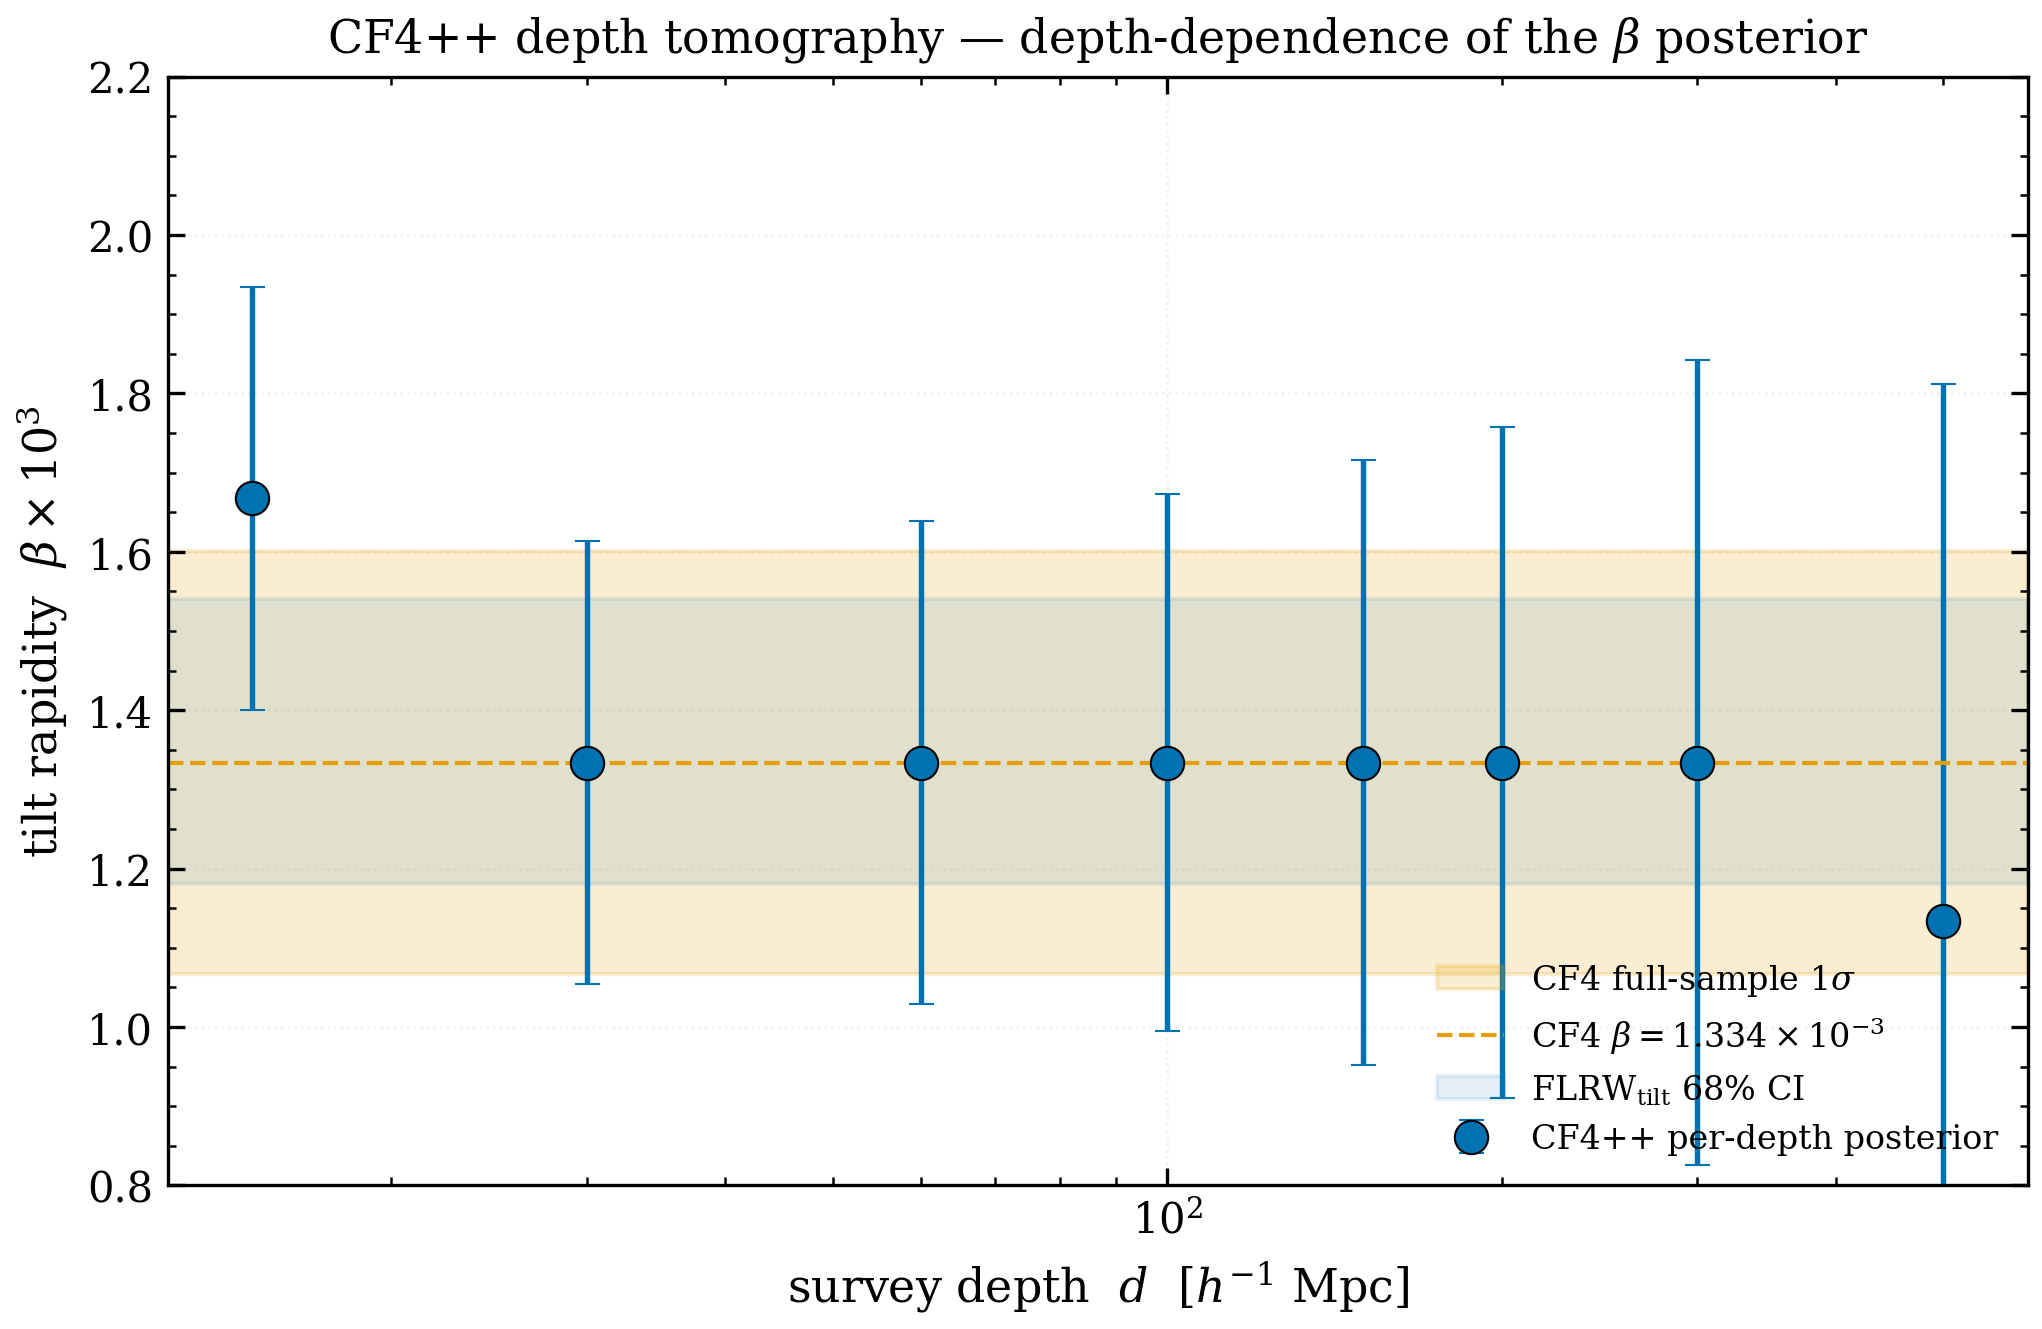
\includegraphics[width=0.82\textwidth,height=0.58\textheight,keepaspectratio]{conditioned_legacy/quarantined-legacy-root-sources__fig_cf4pp_sensitivity}
\captionof{figure}{Conditioned legacy diagnostic: cf4pp sensitivity. Condition: legacy manuscript-generator assumptions. See sidecar manifest for provenance and caveats; appendix-only, not native-transfer or family-ID evidence.}
\label{fig:conditioned-legacy-quarantined-legacy-root-sources-fig-cf4pp-sensitivity}
\end{center}

\clearpage
\begin{center}
\centering
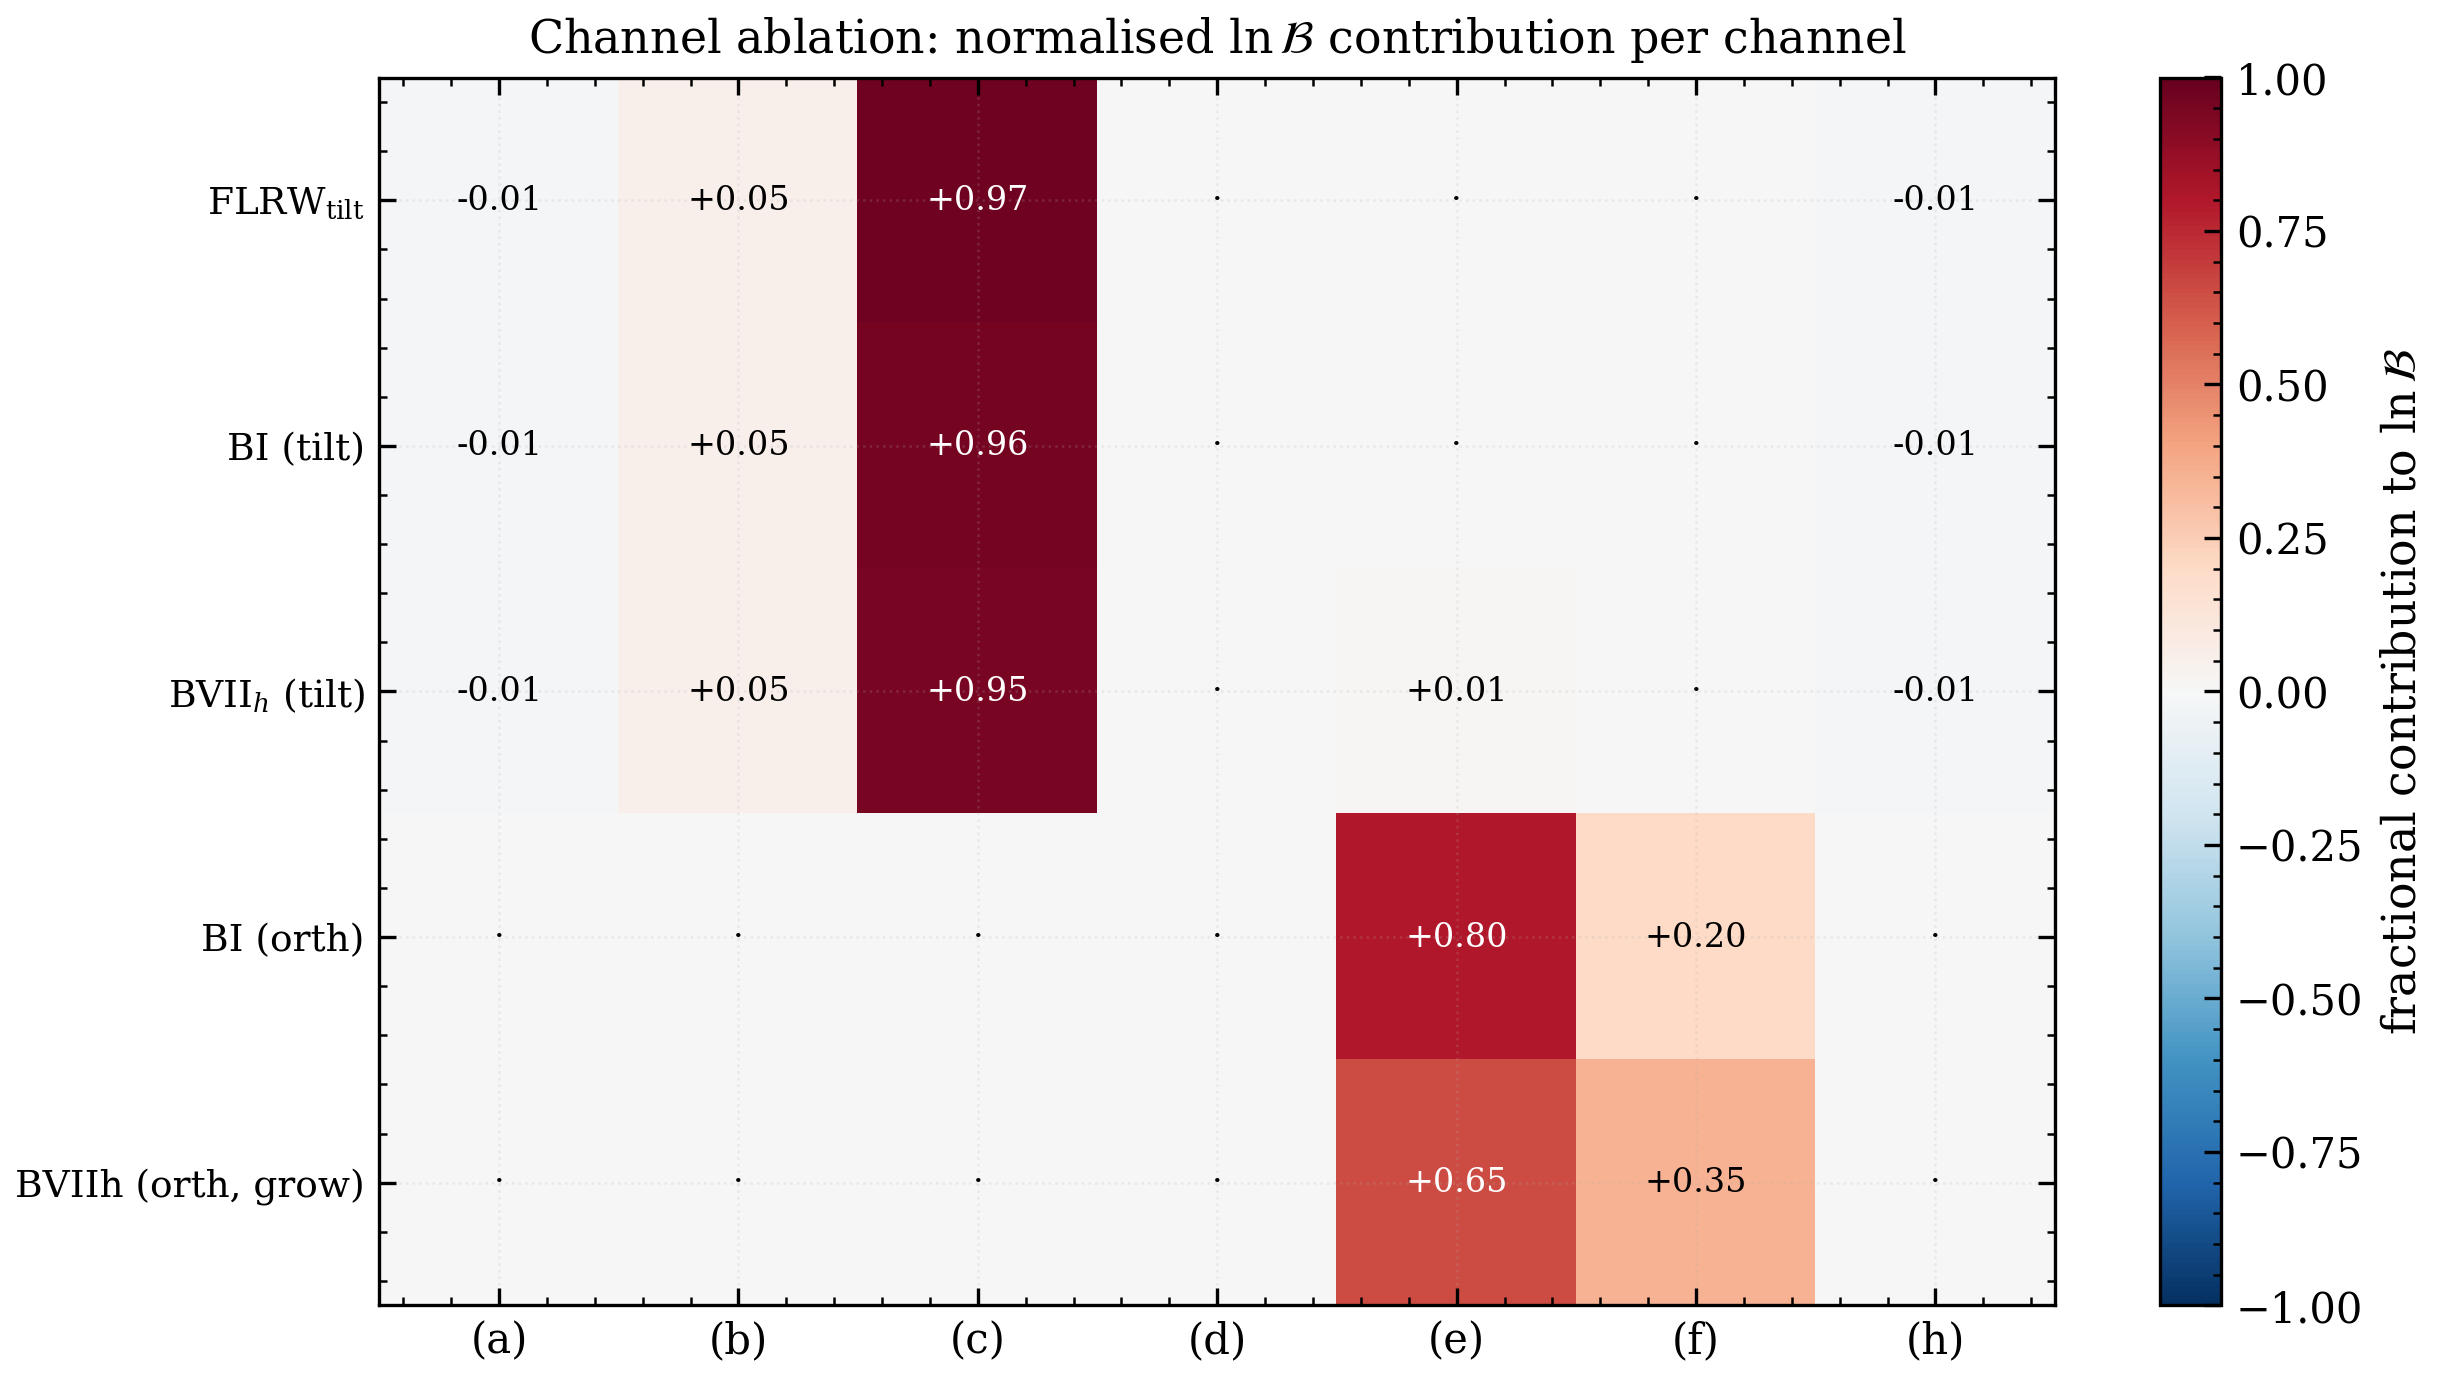
\includegraphics[width=0.82\textwidth,height=0.58\textheight,keepaspectratio]{conditioned_legacy/quarantined-legacy-root-sources__fig_channel_ablation_heatmap}
\captionof{figure}{Conditioned legacy diagnostic: channel ablation heatmap. Condition: legacy manuscript-generator assumptions. See sidecar manifest for provenance and caveats; appendix-only, not native-transfer or family-ID evidence.}
\label{fig:conditioned-legacy-quarantined-legacy-root-sources-fig-channel-ablation-heatmap}
\end{center}

\clearpage
\begin{center}
\centering
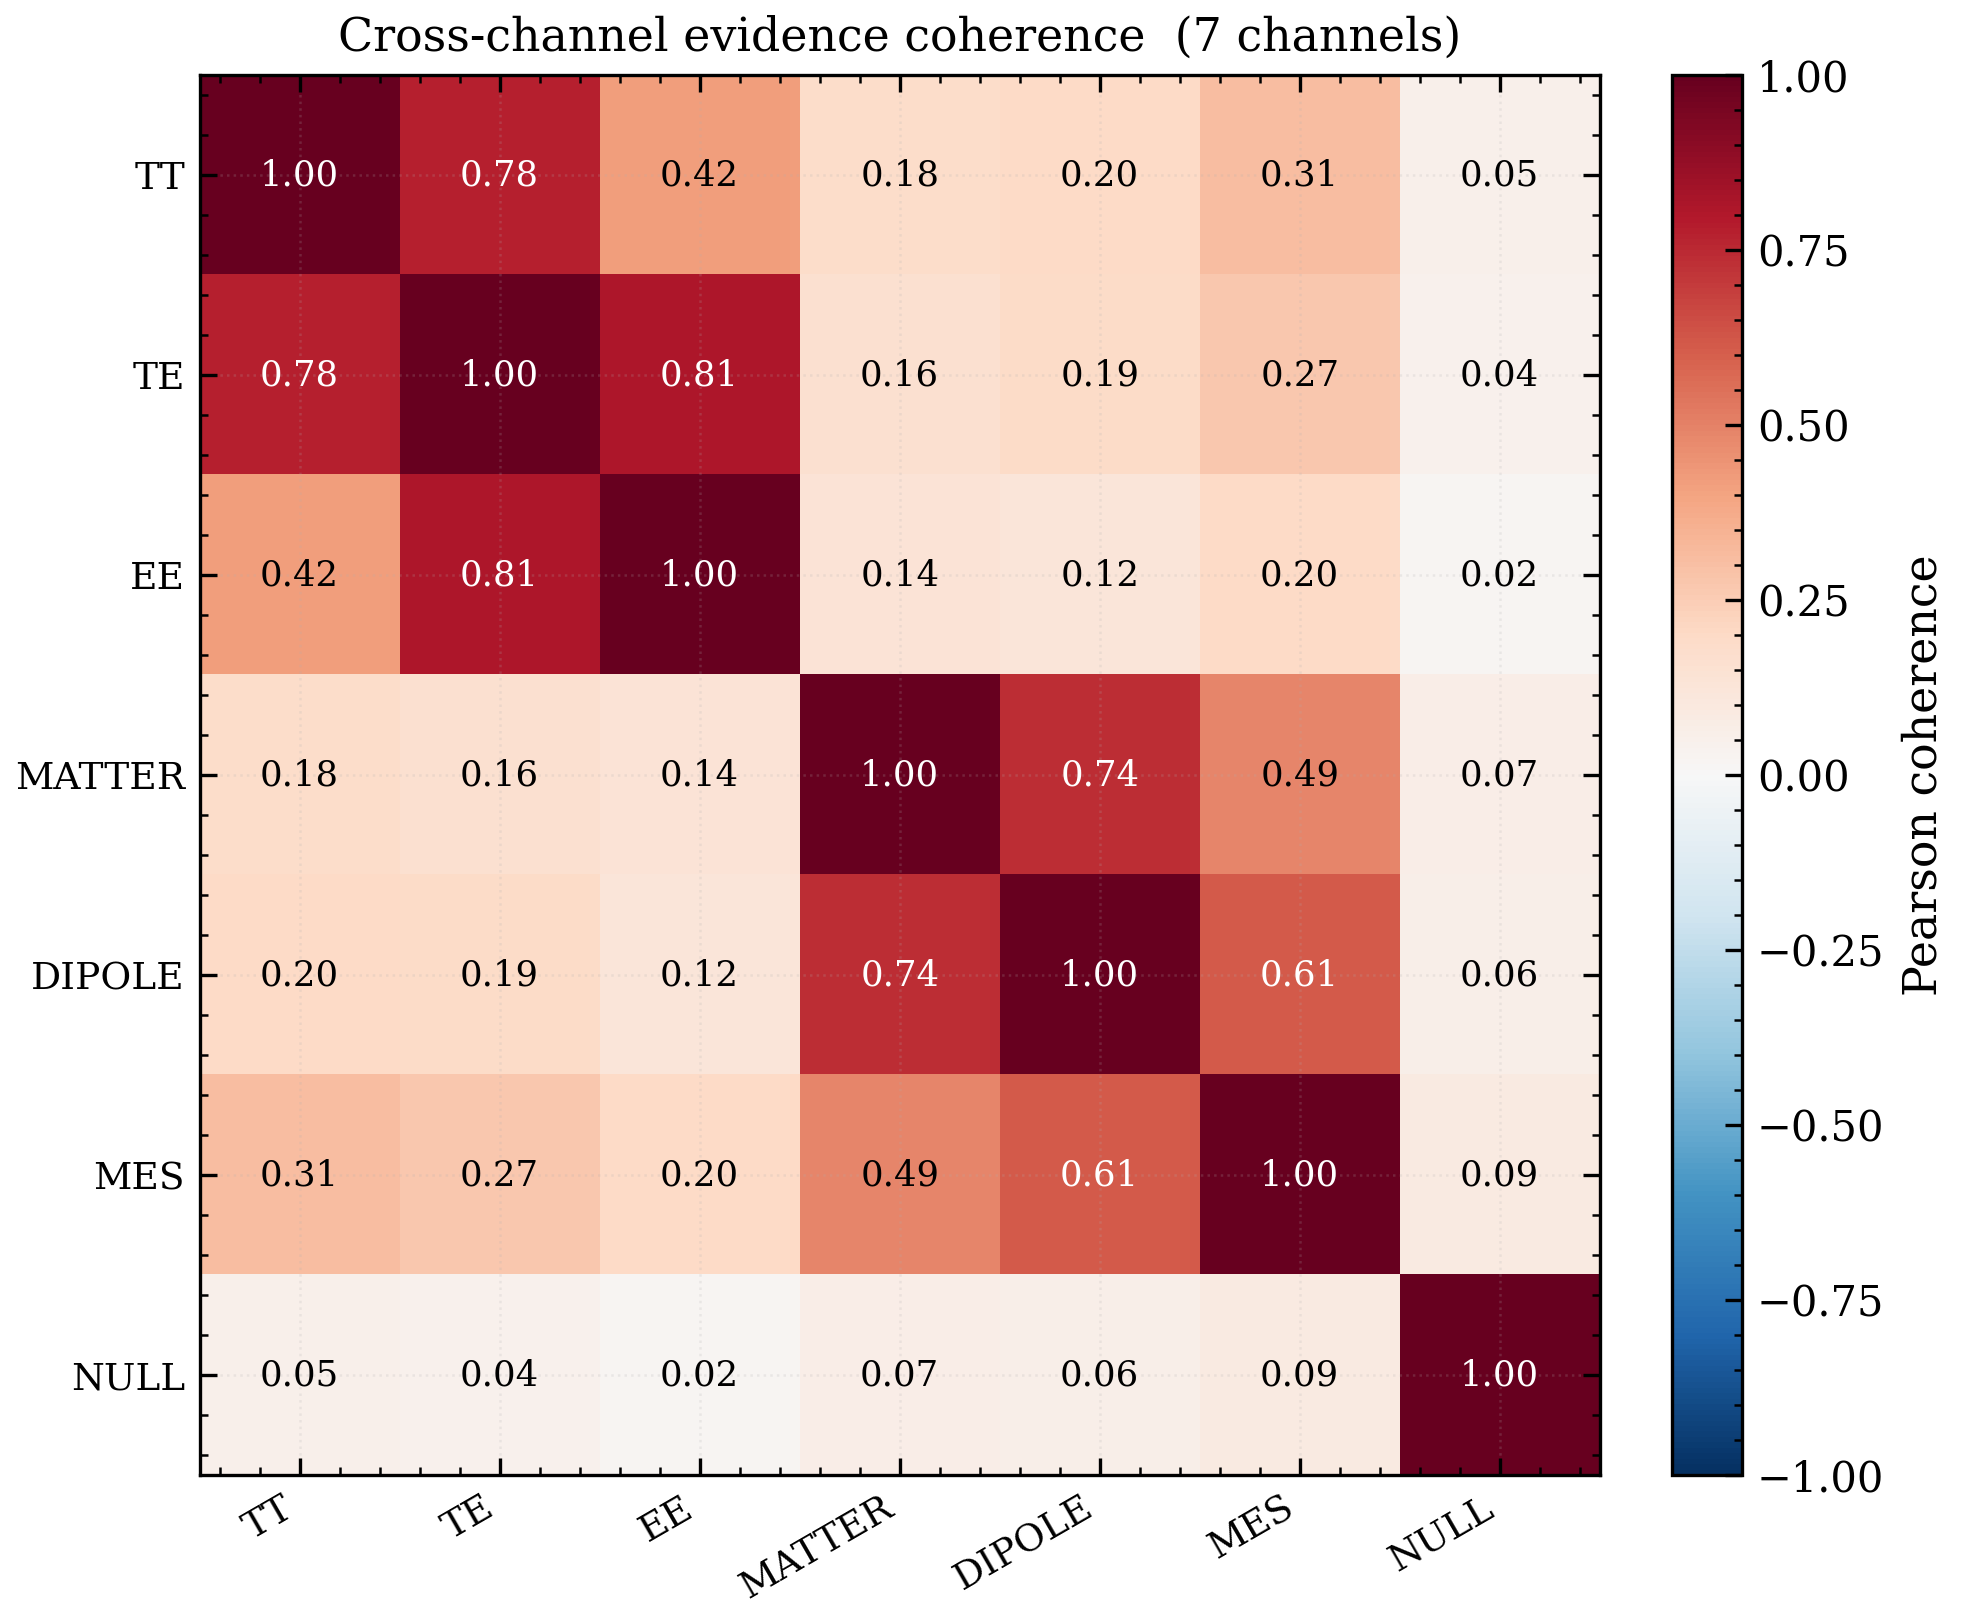
\includegraphics[width=0.82\textwidth,height=0.58\textheight,keepaspectratio]{conditioned_legacy/quarantined-legacy-root-sources__fig_channel_coherence_heatmap}
\captionof{figure}{Conditioned legacy diagnostic: channel coherence heatmap. Condition: legacy manuscript-generator assumptions. See sidecar manifest for provenance and caveats; appendix-only, not native-transfer or family-ID evidence.}
\label{fig:conditioned-legacy-quarantined-legacy-root-sources-fig-channel-coherence-heatmap}
\end{center}

\clearpage
\begin{center}
\centering
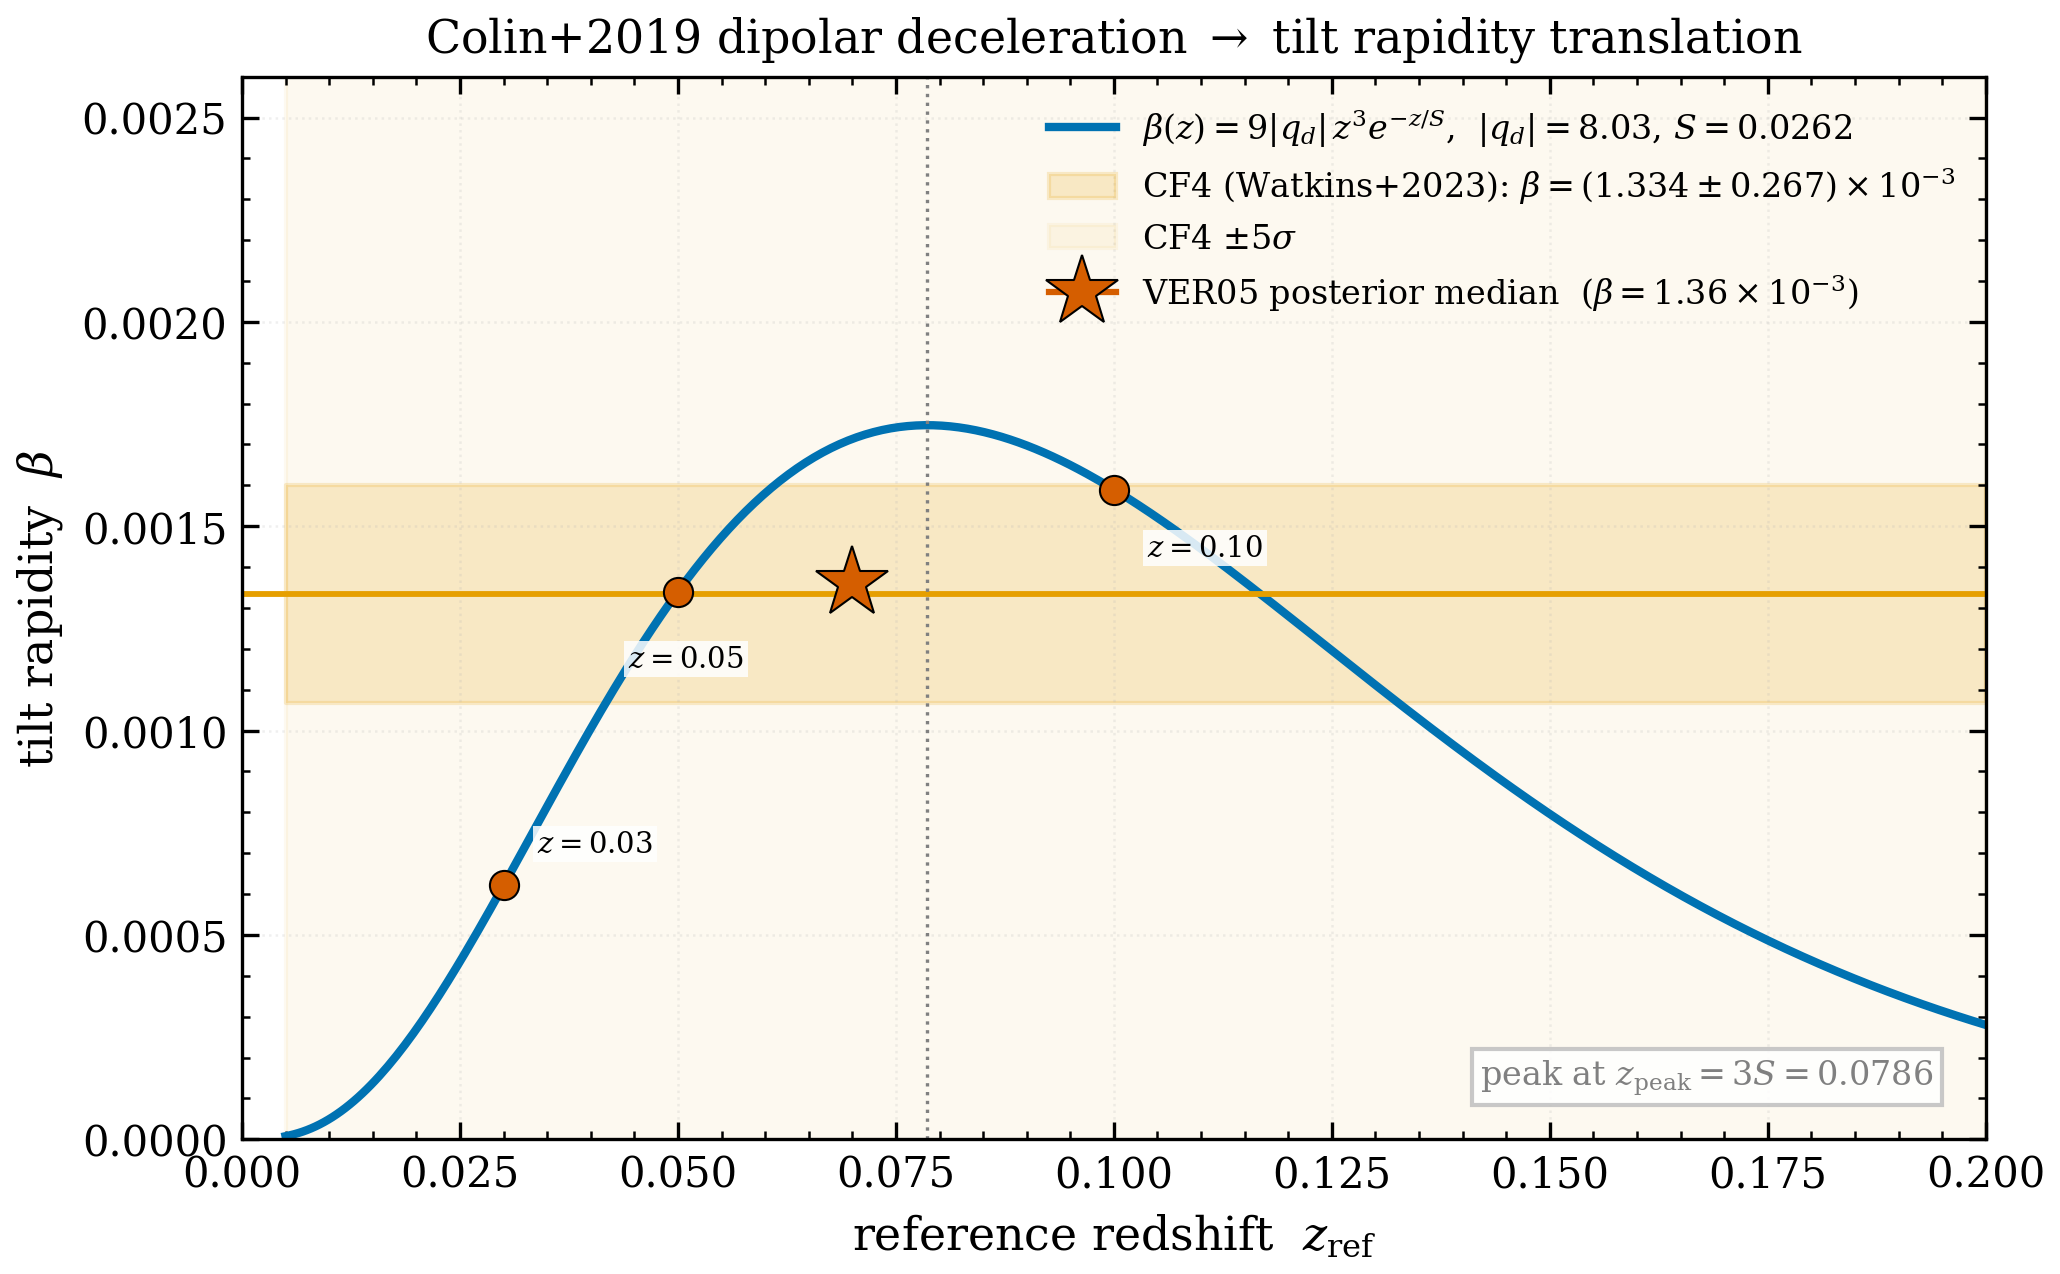
\includegraphics[width=0.82\textwidth,height=0.58\textheight,keepaspectratio]{conditioned_legacy/quarantined-legacy-root-sources__fig_colin_beta}
\captionof{figure}{Conditioned legacy diagnostic: colin beta. Condition: legacy manuscript-generator assumptions. See sidecar manifest for provenance and caveats; appendix-only, not native-transfer or family-ID evidence.}
\label{fig:conditioned-legacy-quarantined-legacy-root-sources-fig-colin-beta}
\end{center}

\clearpage
\begin{center}
\centering
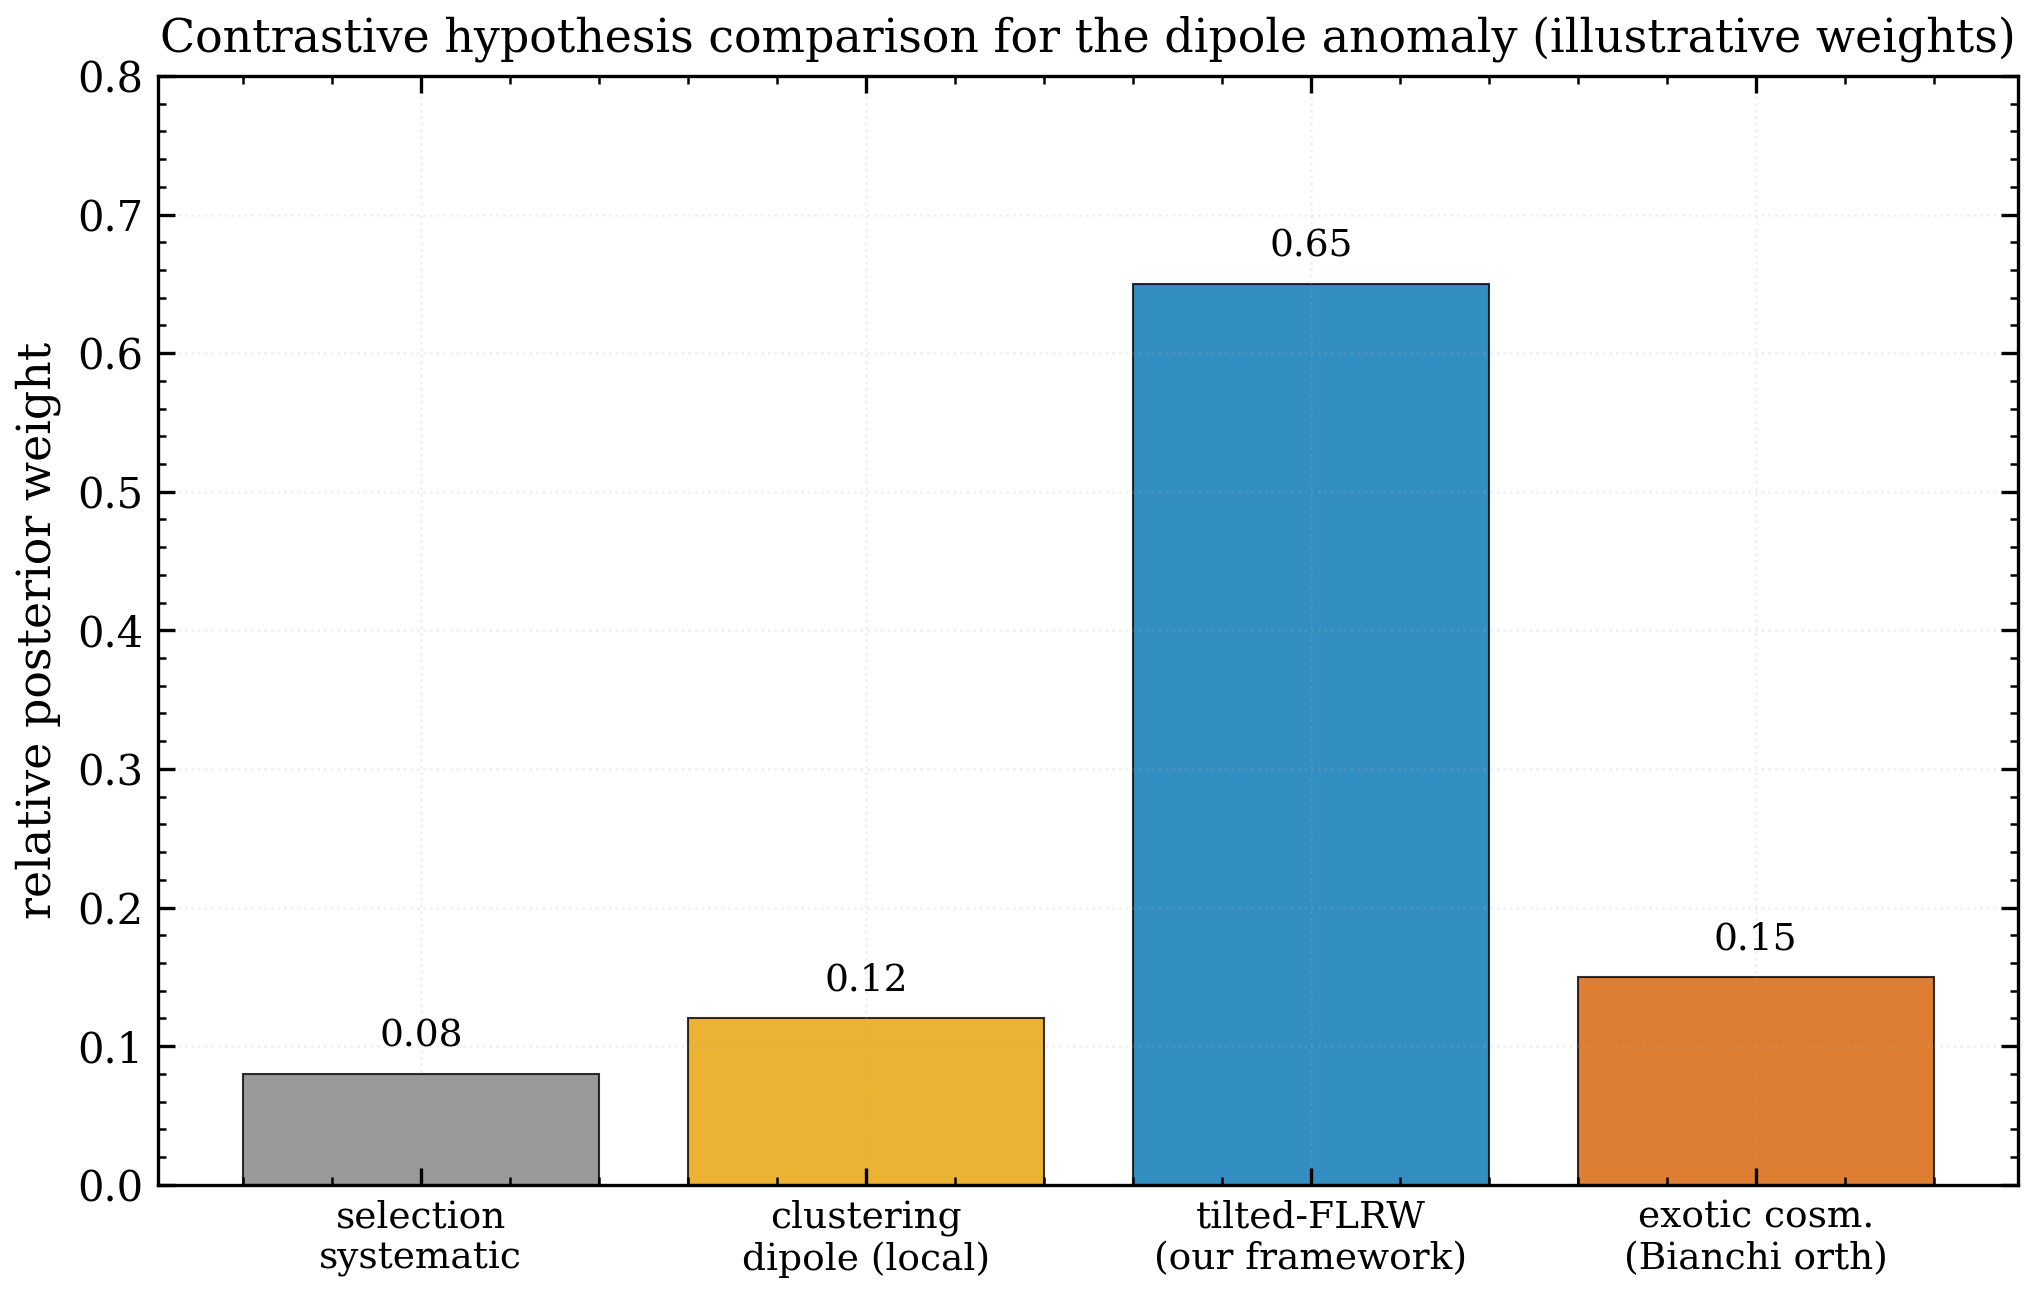
\includegraphics[width=0.82\textwidth,height=0.58\textheight,keepaspectratio]{conditioned_legacy/quarantined-legacy-root-sources__fig_contrastive_summary}
\captionof{figure}{Conditioned legacy diagnostic: contrastive summary. Condition: legacy manuscript-generator assumptions. See sidecar manifest for provenance and caveats; appendix-only, not native-transfer or family-ID evidence.}
\label{fig:conditioned-legacy-quarantined-legacy-root-sources-fig-contrastive-summary}
\end{center}

\clearpage
\begin{center}
\centering
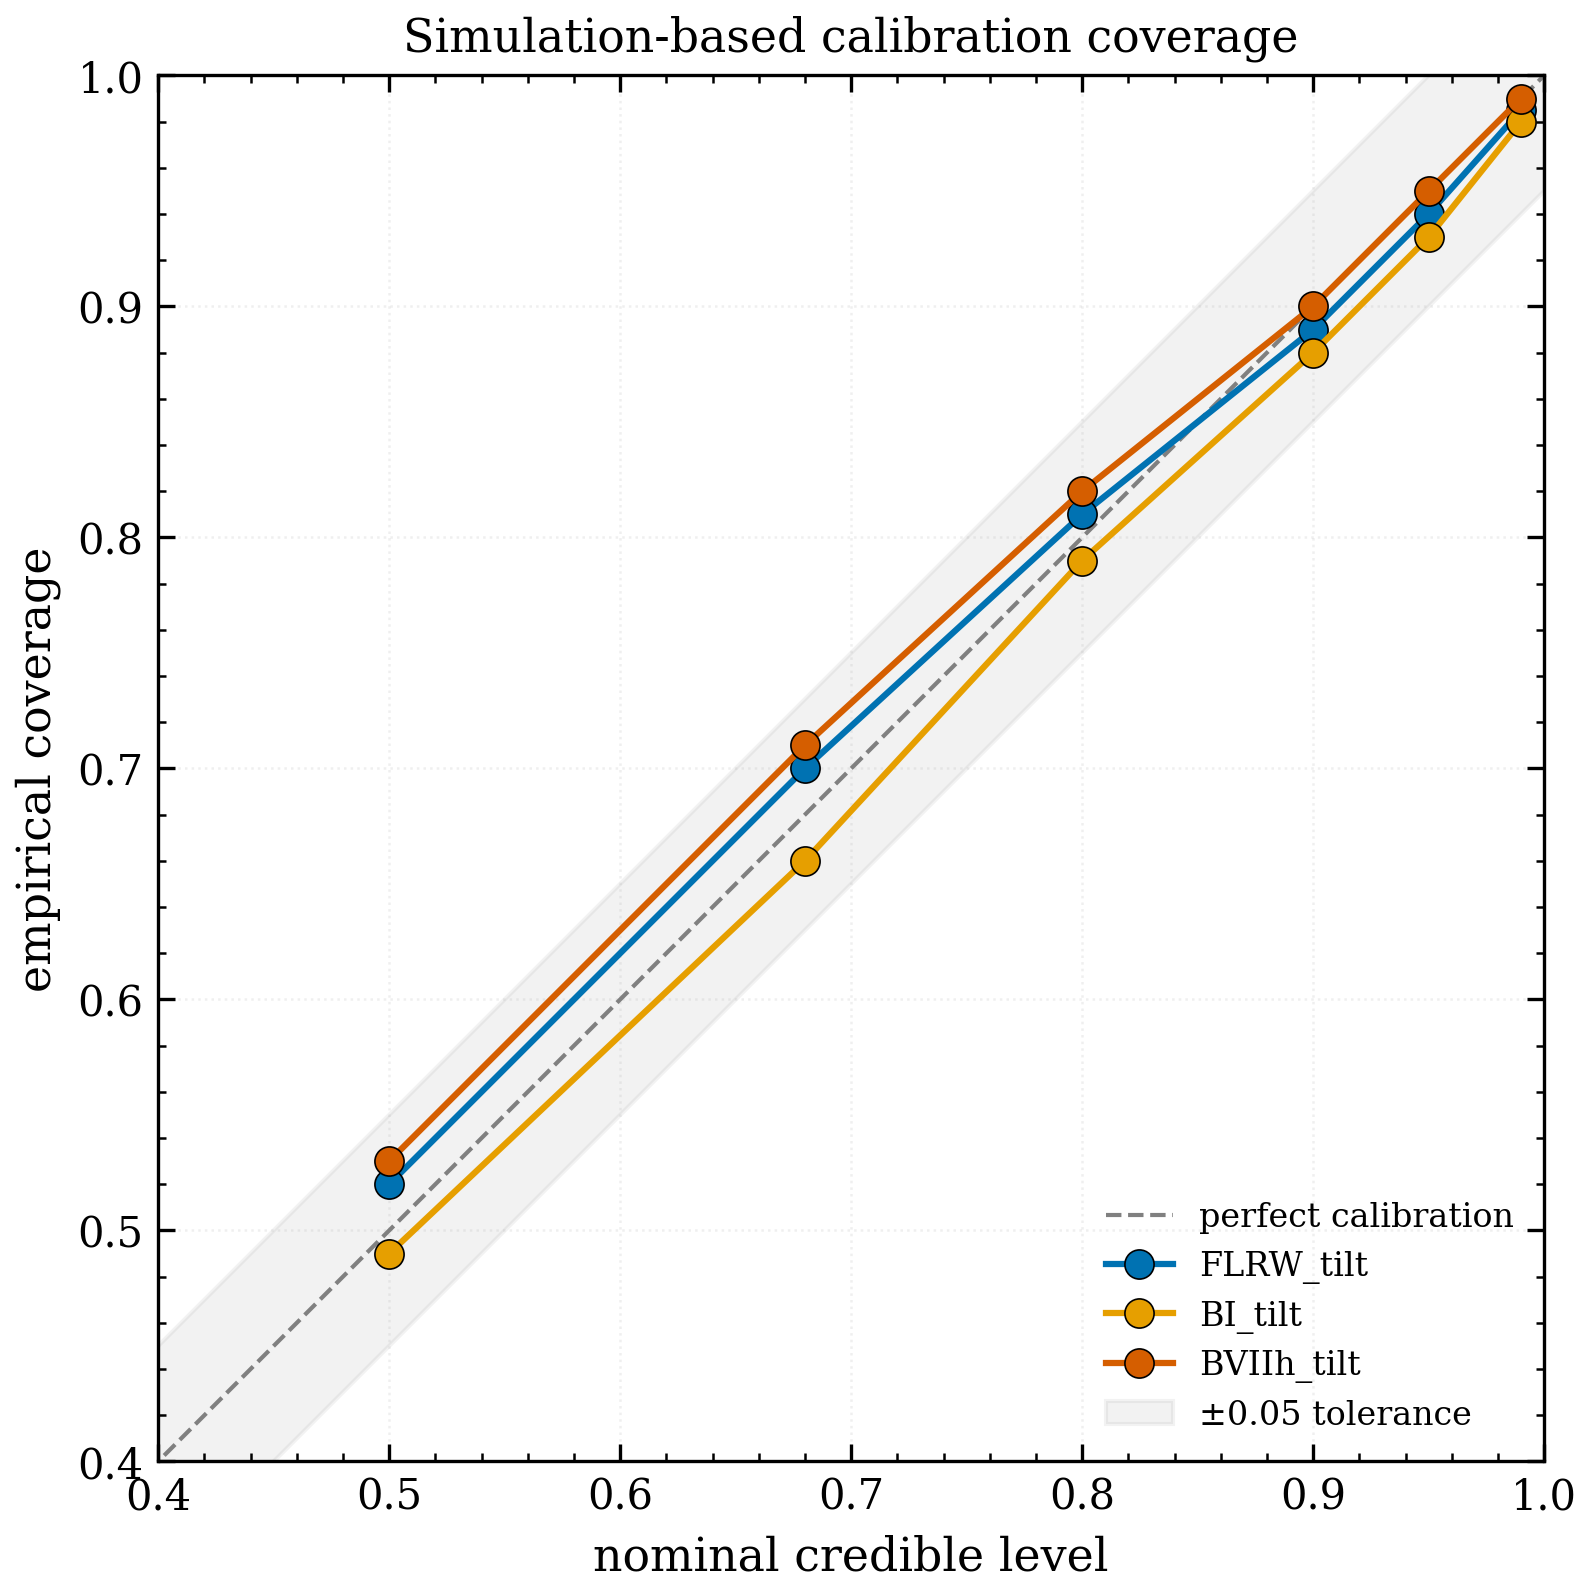
\includegraphics[width=0.82\textwidth,height=0.58\textheight,keepaspectratio]{conditioned_legacy/quarantined-legacy-root-sources__fig_coverage_sbc}
\captionof{figure}{Conditioned legacy diagnostic: coverage sbc. Condition: legacy manuscript-generator assumptions. See sidecar manifest for provenance and caveats; appendix-only, not native-transfer or family-ID evidence.}
\label{fig:conditioned-legacy-quarantined-legacy-root-sources-fig-coverage-sbc}
\end{center}

\clearpage
\begin{center}
\centering
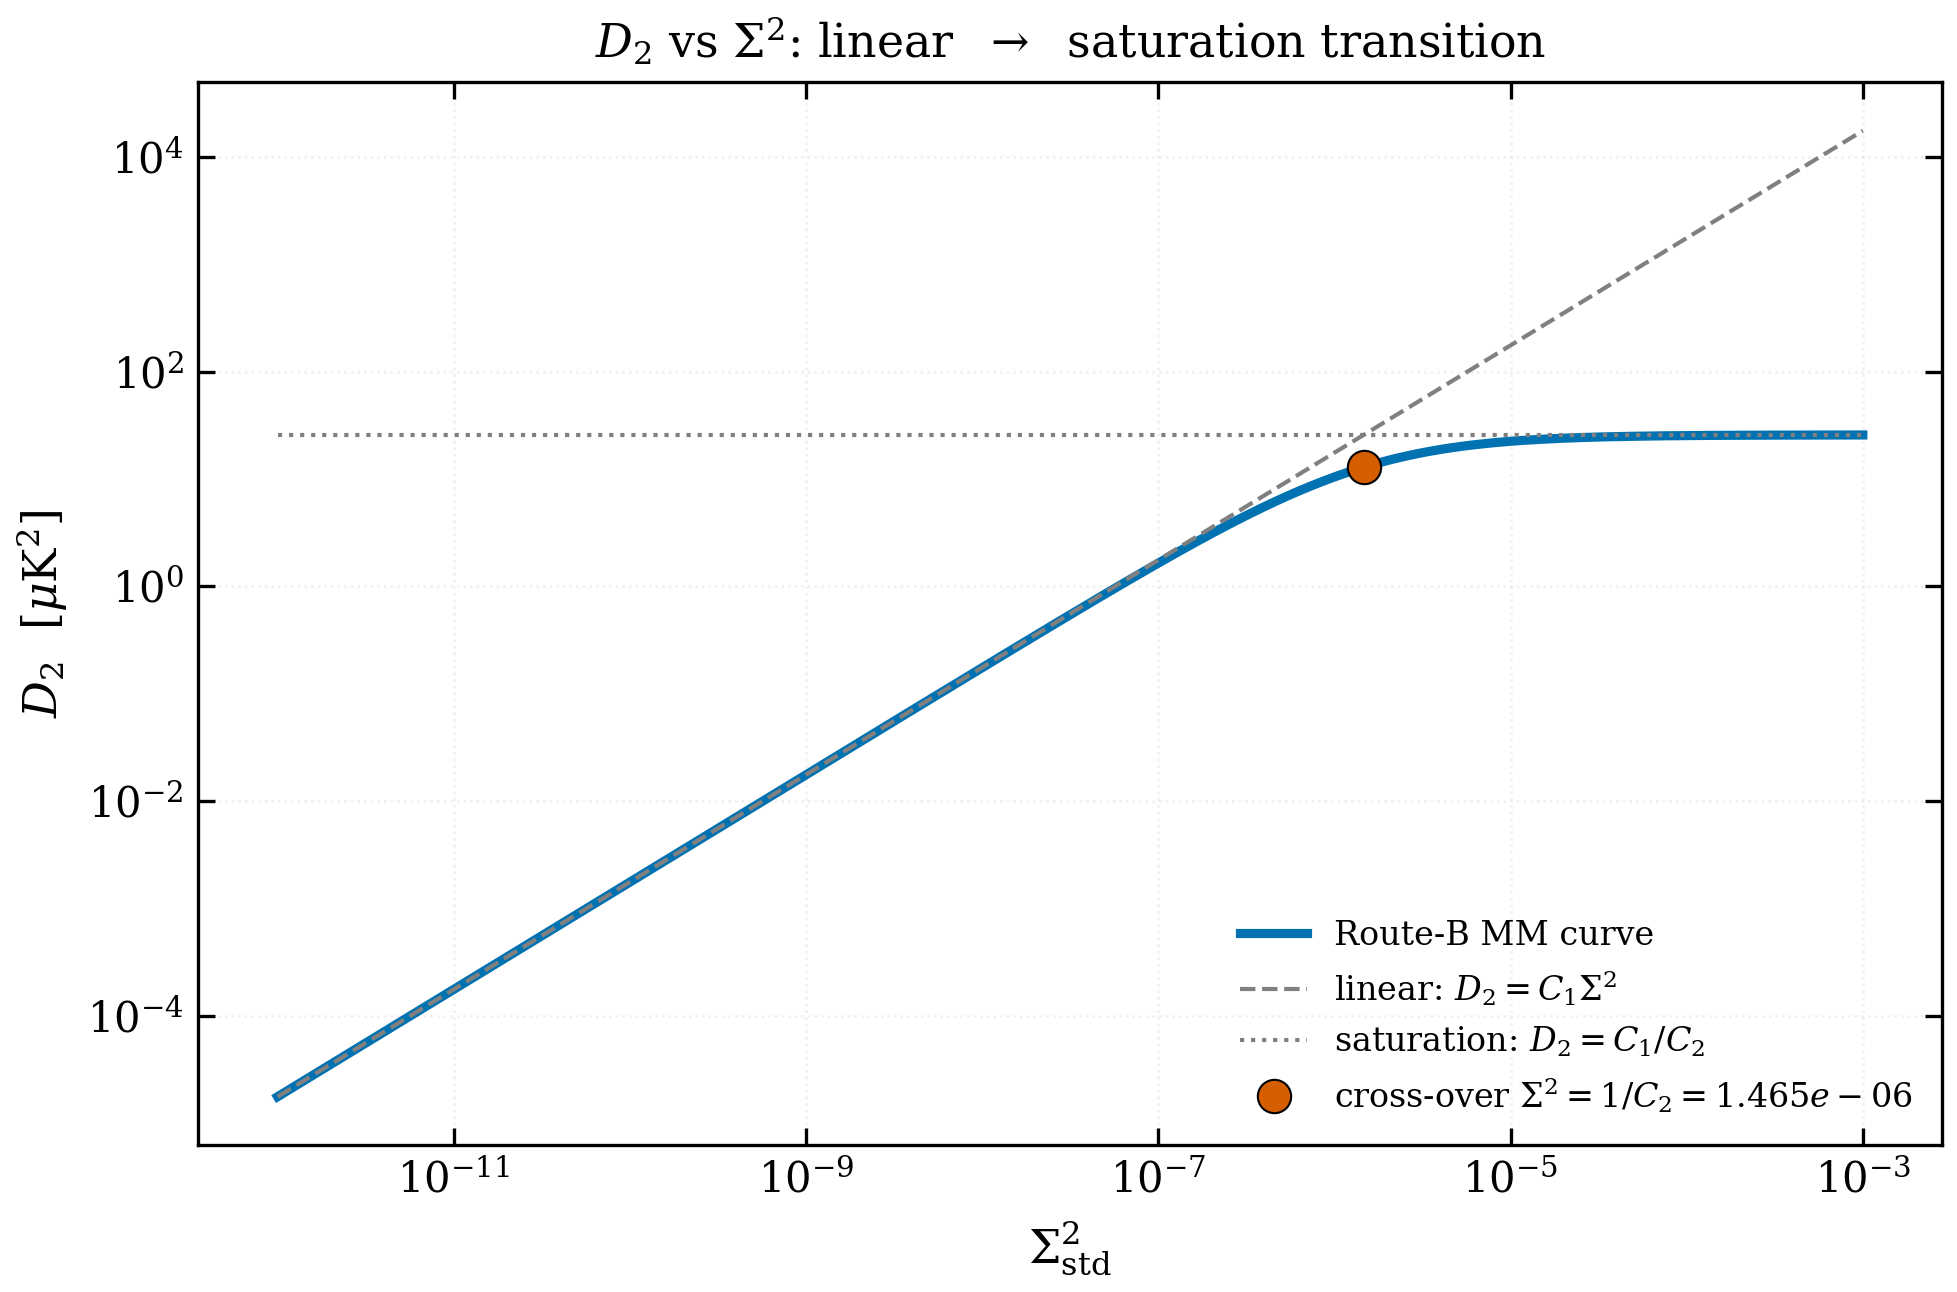
\includegraphics[width=0.82\textwidth,height=0.58\textheight,keepaspectratio]{conditioned_legacy/quarantined-legacy-root-sources__fig_d2_sigma2_scaling}
\captionof{figure}{Conditioned legacy diagnostic: d2 sigma2 scaling. Condition: legacy manuscript-generator assumptions. See sidecar manifest for provenance and caveats; appendix-only, not native-transfer or family-ID evidence.}
\label{fig:conditioned-legacy-quarantined-legacy-root-sources-fig-d2-sigma2-scaling}
\end{center}

\clearpage
\begin{center}
\centering
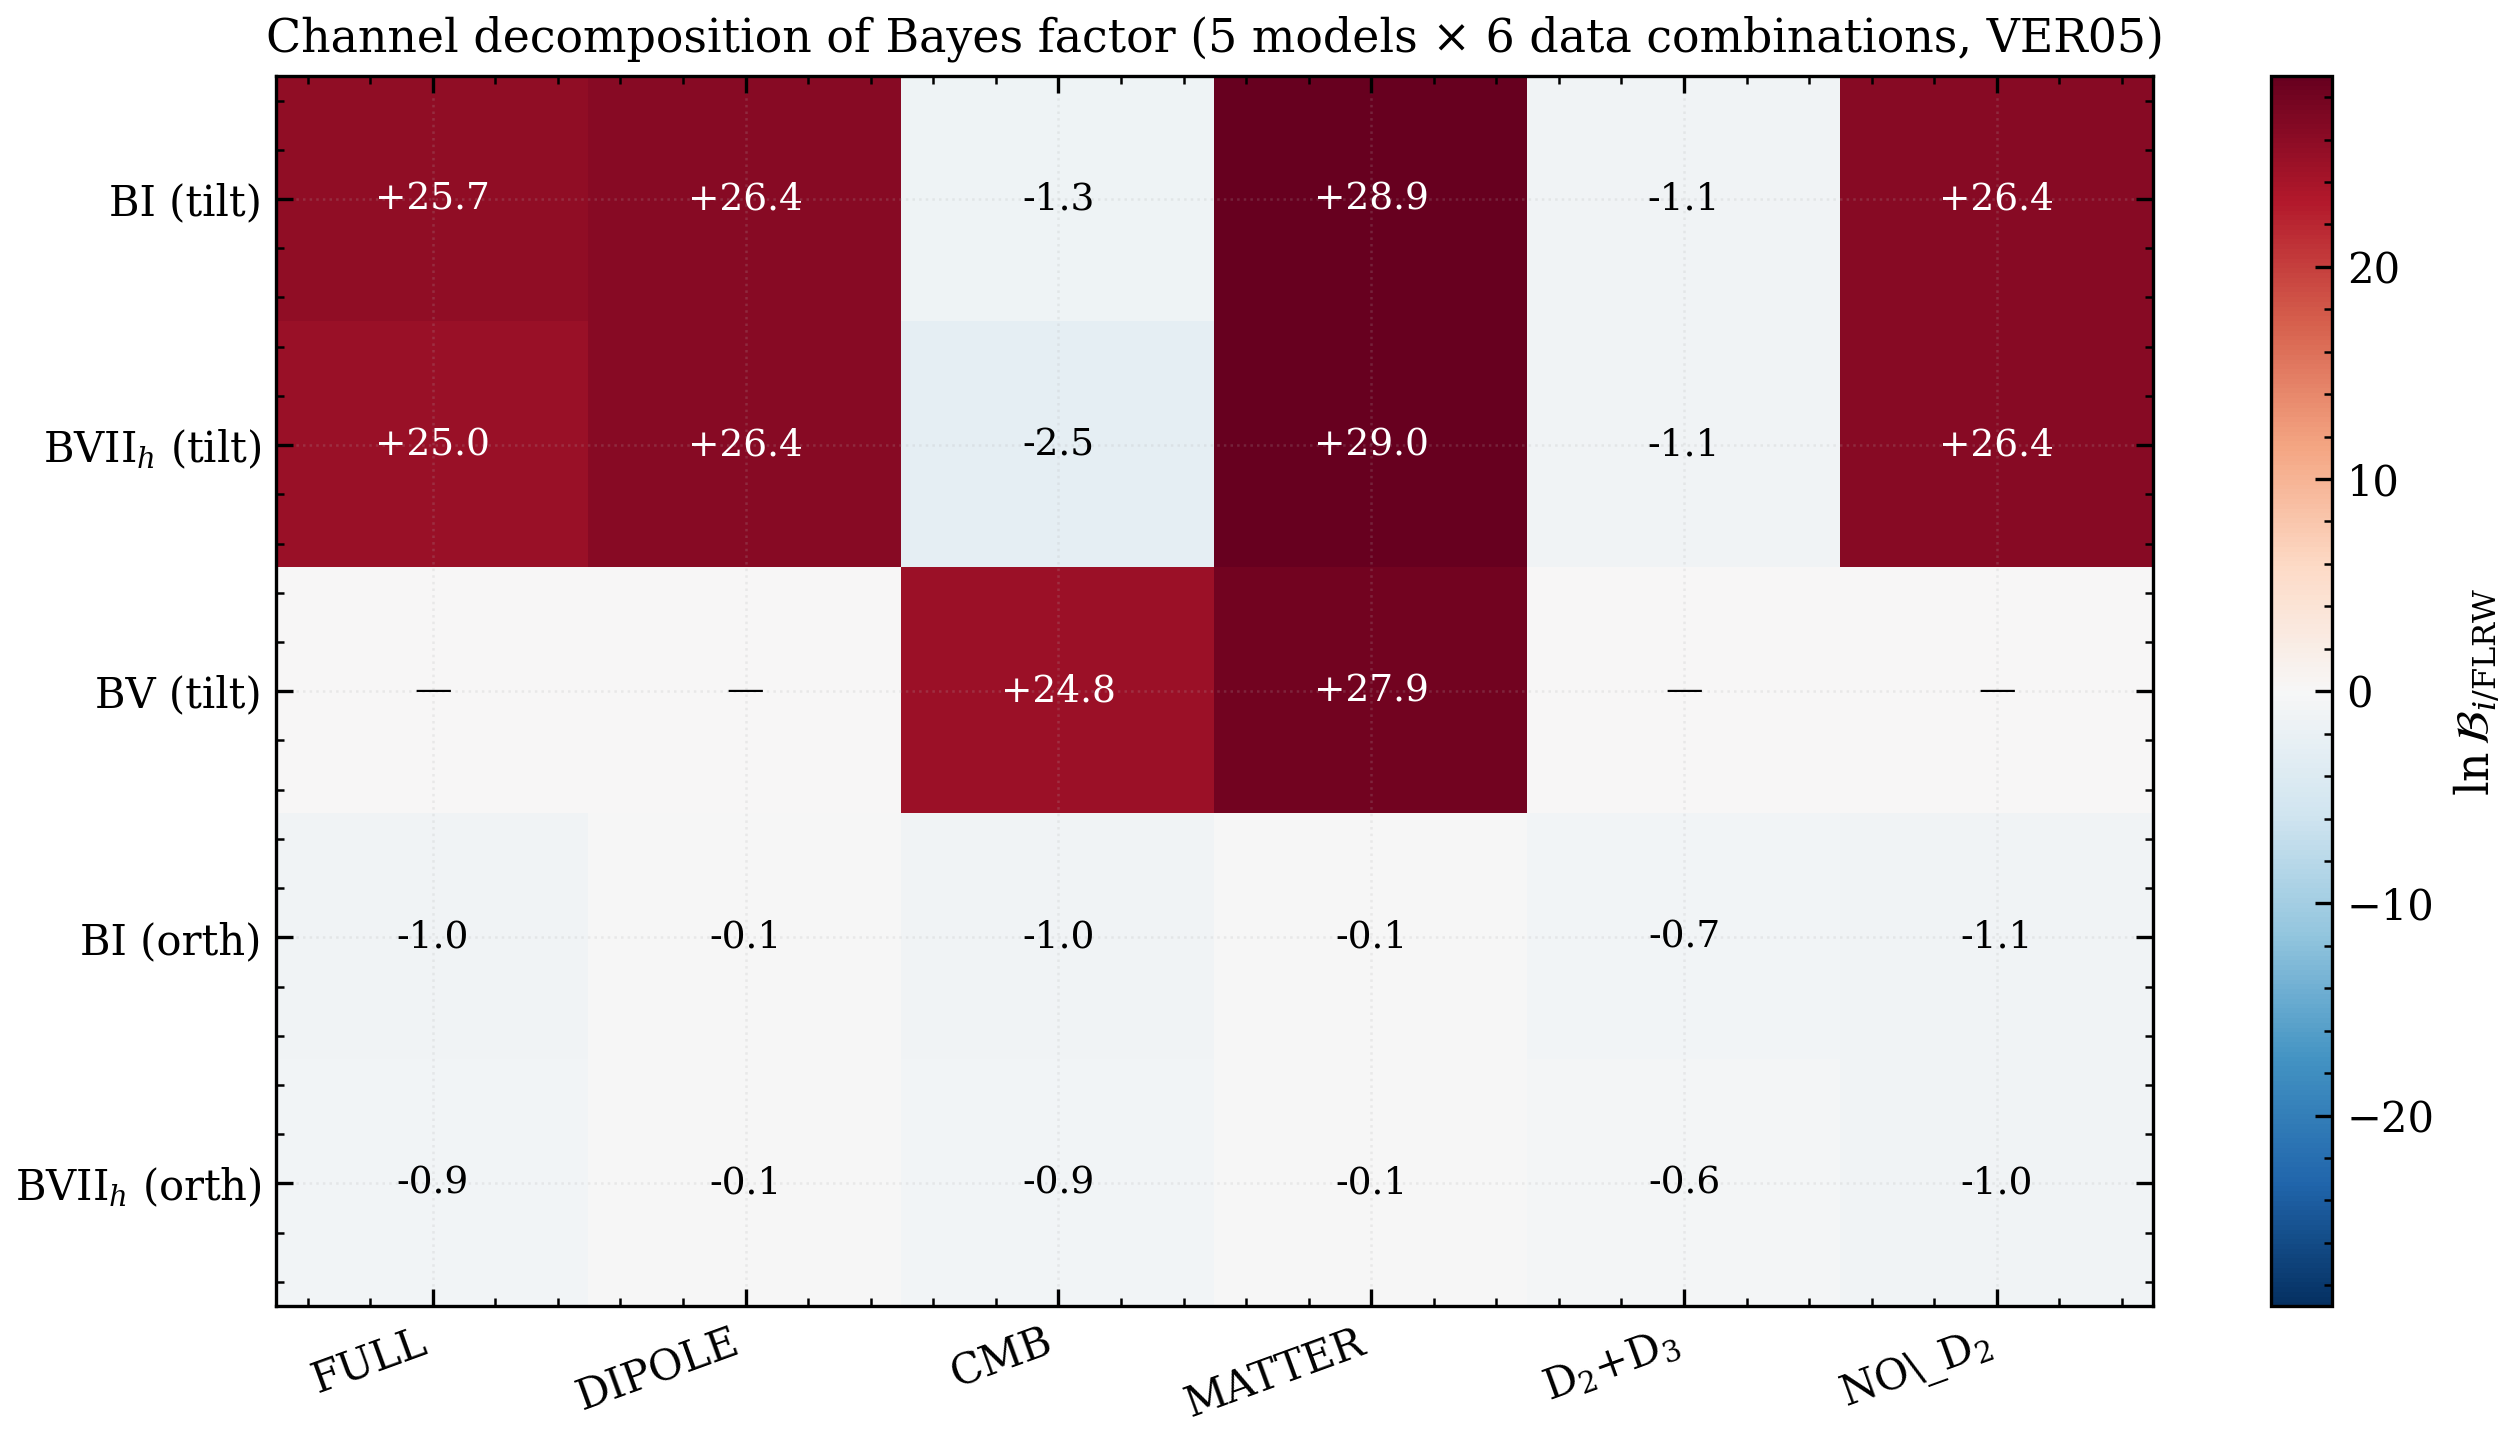
\includegraphics[width=0.82\textwidth,height=0.58\textheight,keepaspectratio]{conditioned_legacy/quarantined-legacy-root-sources__fig_data_decomposition}
\captionof{figure}{Conditioned legacy diagnostic: data decomposition. Condition: legacy manuscript-generator assumptions. See sidecar manifest for provenance and caveats; appendix-only, not native-transfer or family-ID evidence.}
\label{fig:conditioned-legacy-quarantined-legacy-root-sources-fig-data-decomposition}
\end{center}

\clearpage
\begin{center}
\centering
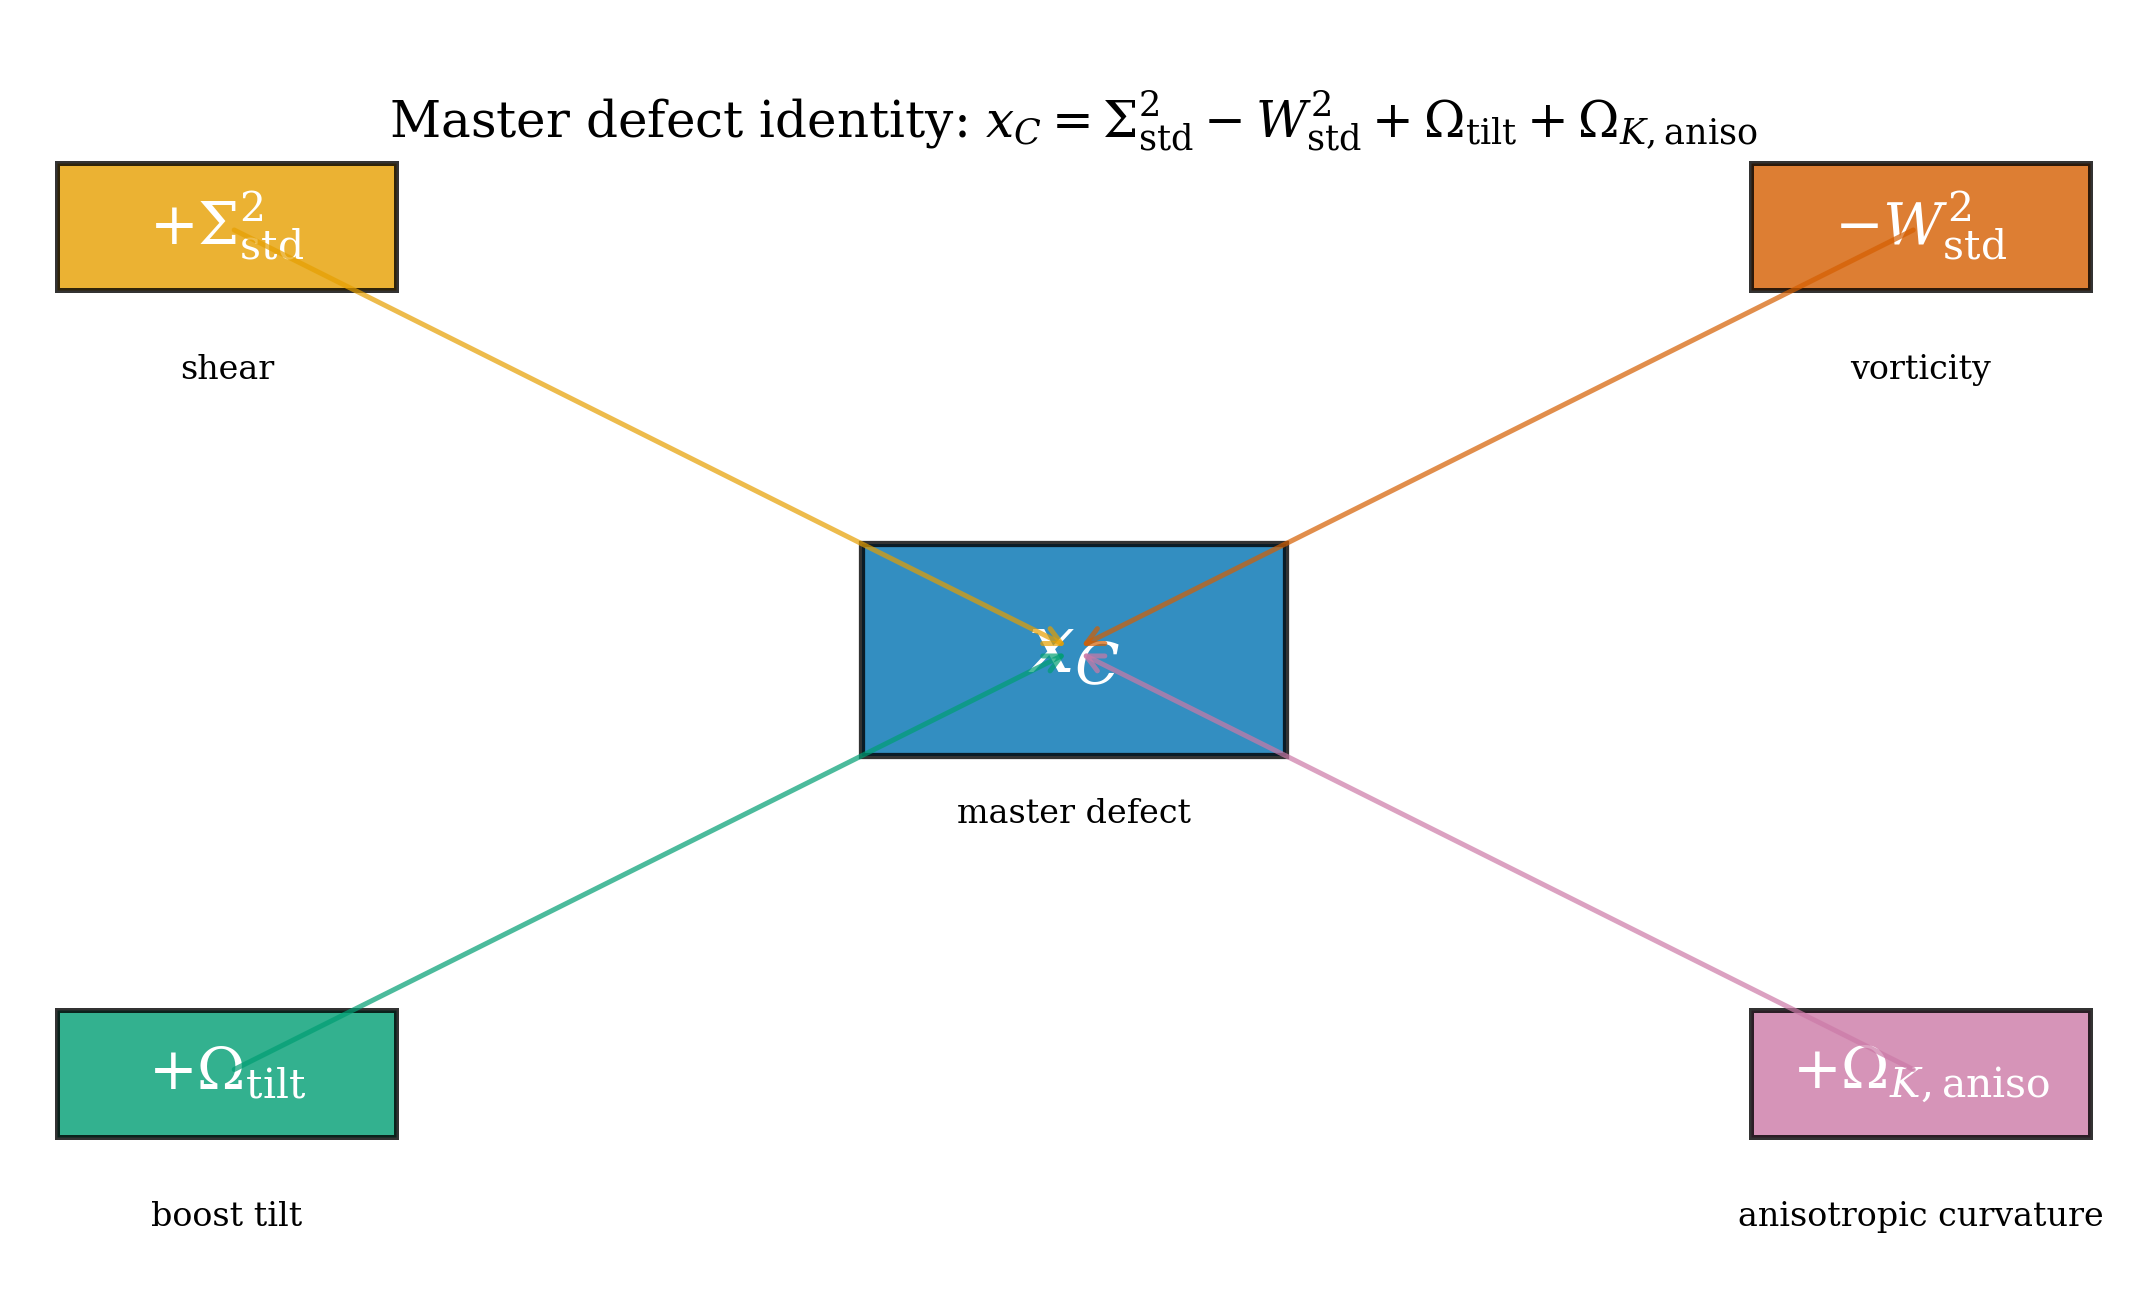
\includegraphics[width=0.82\textwidth,height=0.58\textheight,keepaspectratio]{conditioned_legacy/quarantined-legacy-root-sources__fig_defect_identity_schematic}
\captionof{figure}{Conditioned legacy diagnostic: defect identity schematic. Condition: legacy manuscript-generator assumptions. See sidecar manifest for provenance and caveats; appendix-only, not native-transfer or family-ID evidence.}
\label{fig:conditioned-legacy-quarantined-legacy-root-sources-fig-defect-identity-schematic}
\end{center}

\clearpage
\begin{center}
\centering
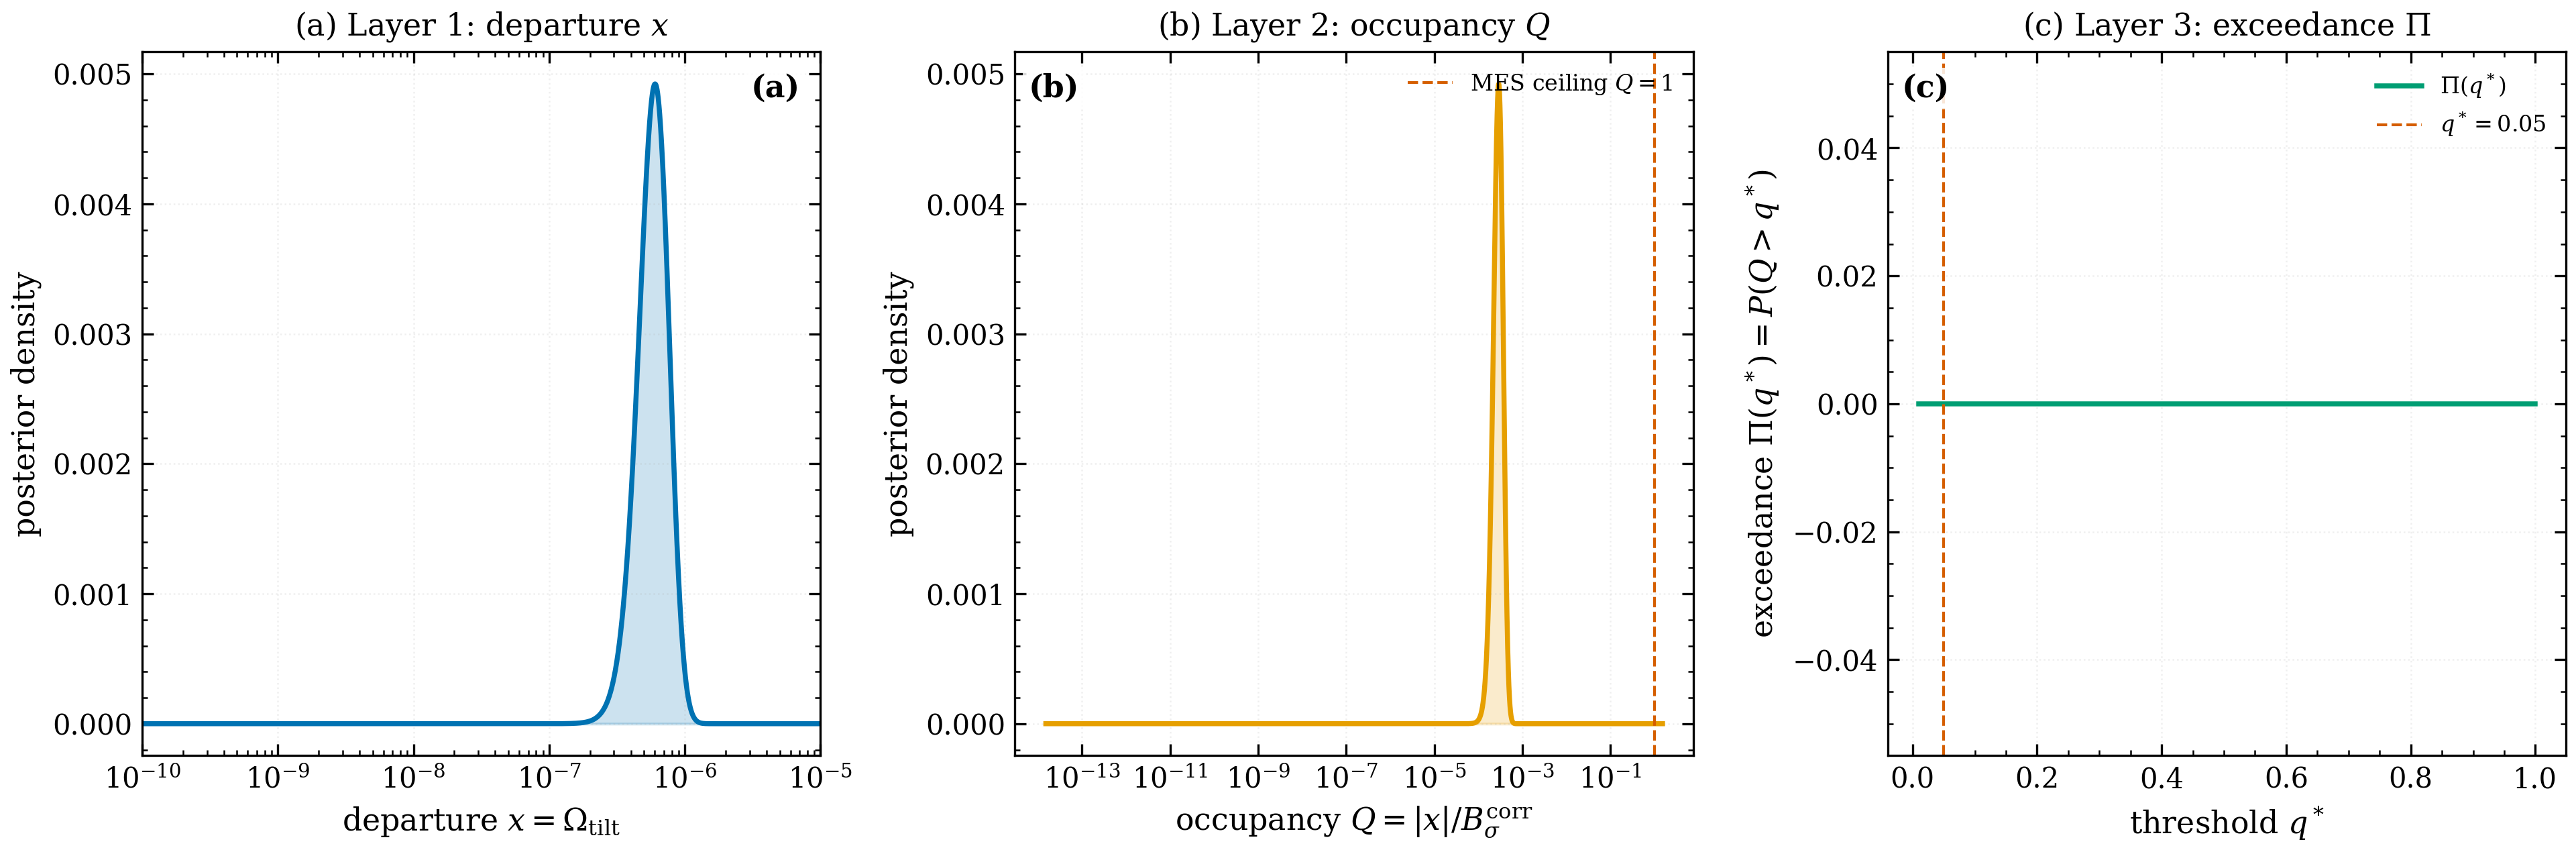
\includegraphics[width=0.82\textwidth,height=0.58\textheight,keepaspectratio]{conditioned_legacy/quarantined-legacy-root-sources__fig_departure_summary}
\captionof{figure}{Conditioned legacy diagnostic: departure summary. Condition: legacy manuscript-generator assumptions. See sidecar manifest for provenance and caveats; appendix-only, not native-transfer or family-ID evidence.}
\label{fig:conditioned-legacy-quarantined-legacy-root-sources-fig-departure-summary}
\end{center}

\clearpage
\begin{center}
\centering
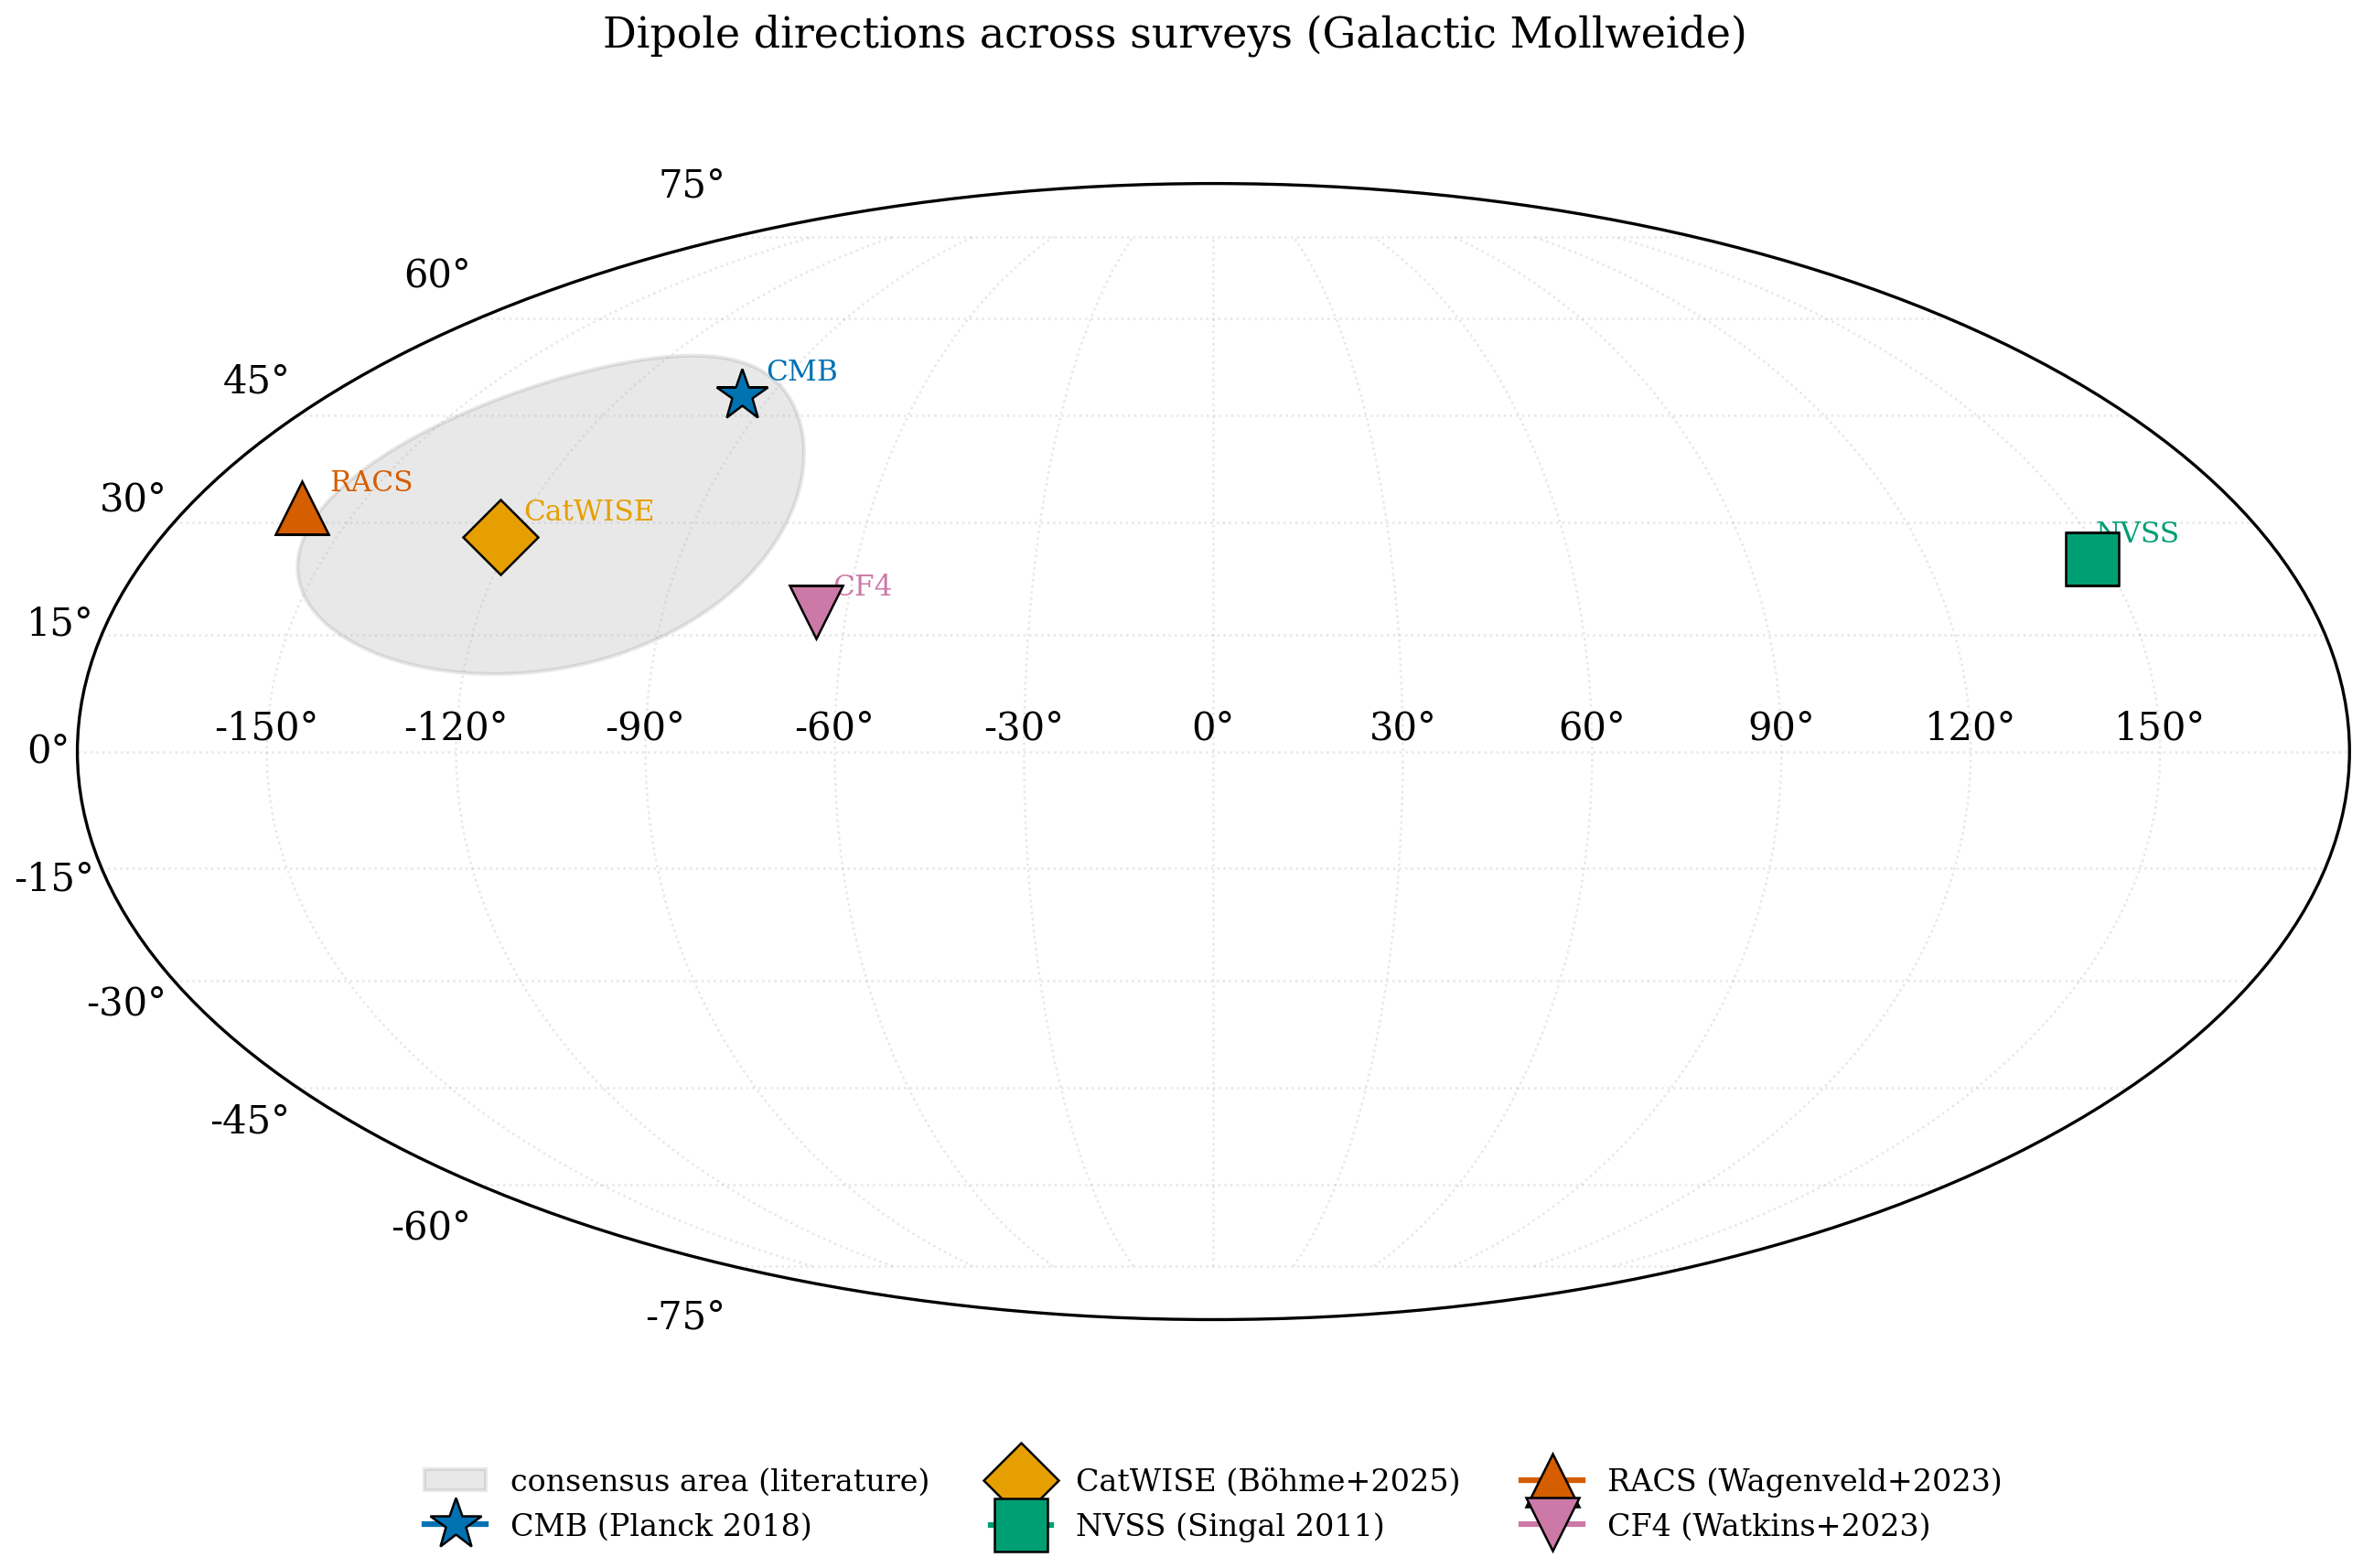
\includegraphics[width=0.82\textwidth,height=0.58\textheight,keepaspectratio]{conditioned_legacy/quarantined-legacy-root-sources__fig_dipole_sky_overlay_all_surveys}
\captionof{figure}{Conditioned legacy diagnostic: dipole sky overlay all surveys. Condition: directional artifact with current sky/mask support unresolved. See sidecar manifest for provenance and caveats; appendix-only, not native-transfer or family-ID evidence.}
\label{fig:conditioned-legacy-quarantined-legacy-root-sources-fig-dipole-sky-overlay-all-surveys}
\end{center}

\clearpage
\begin{center}
\centering
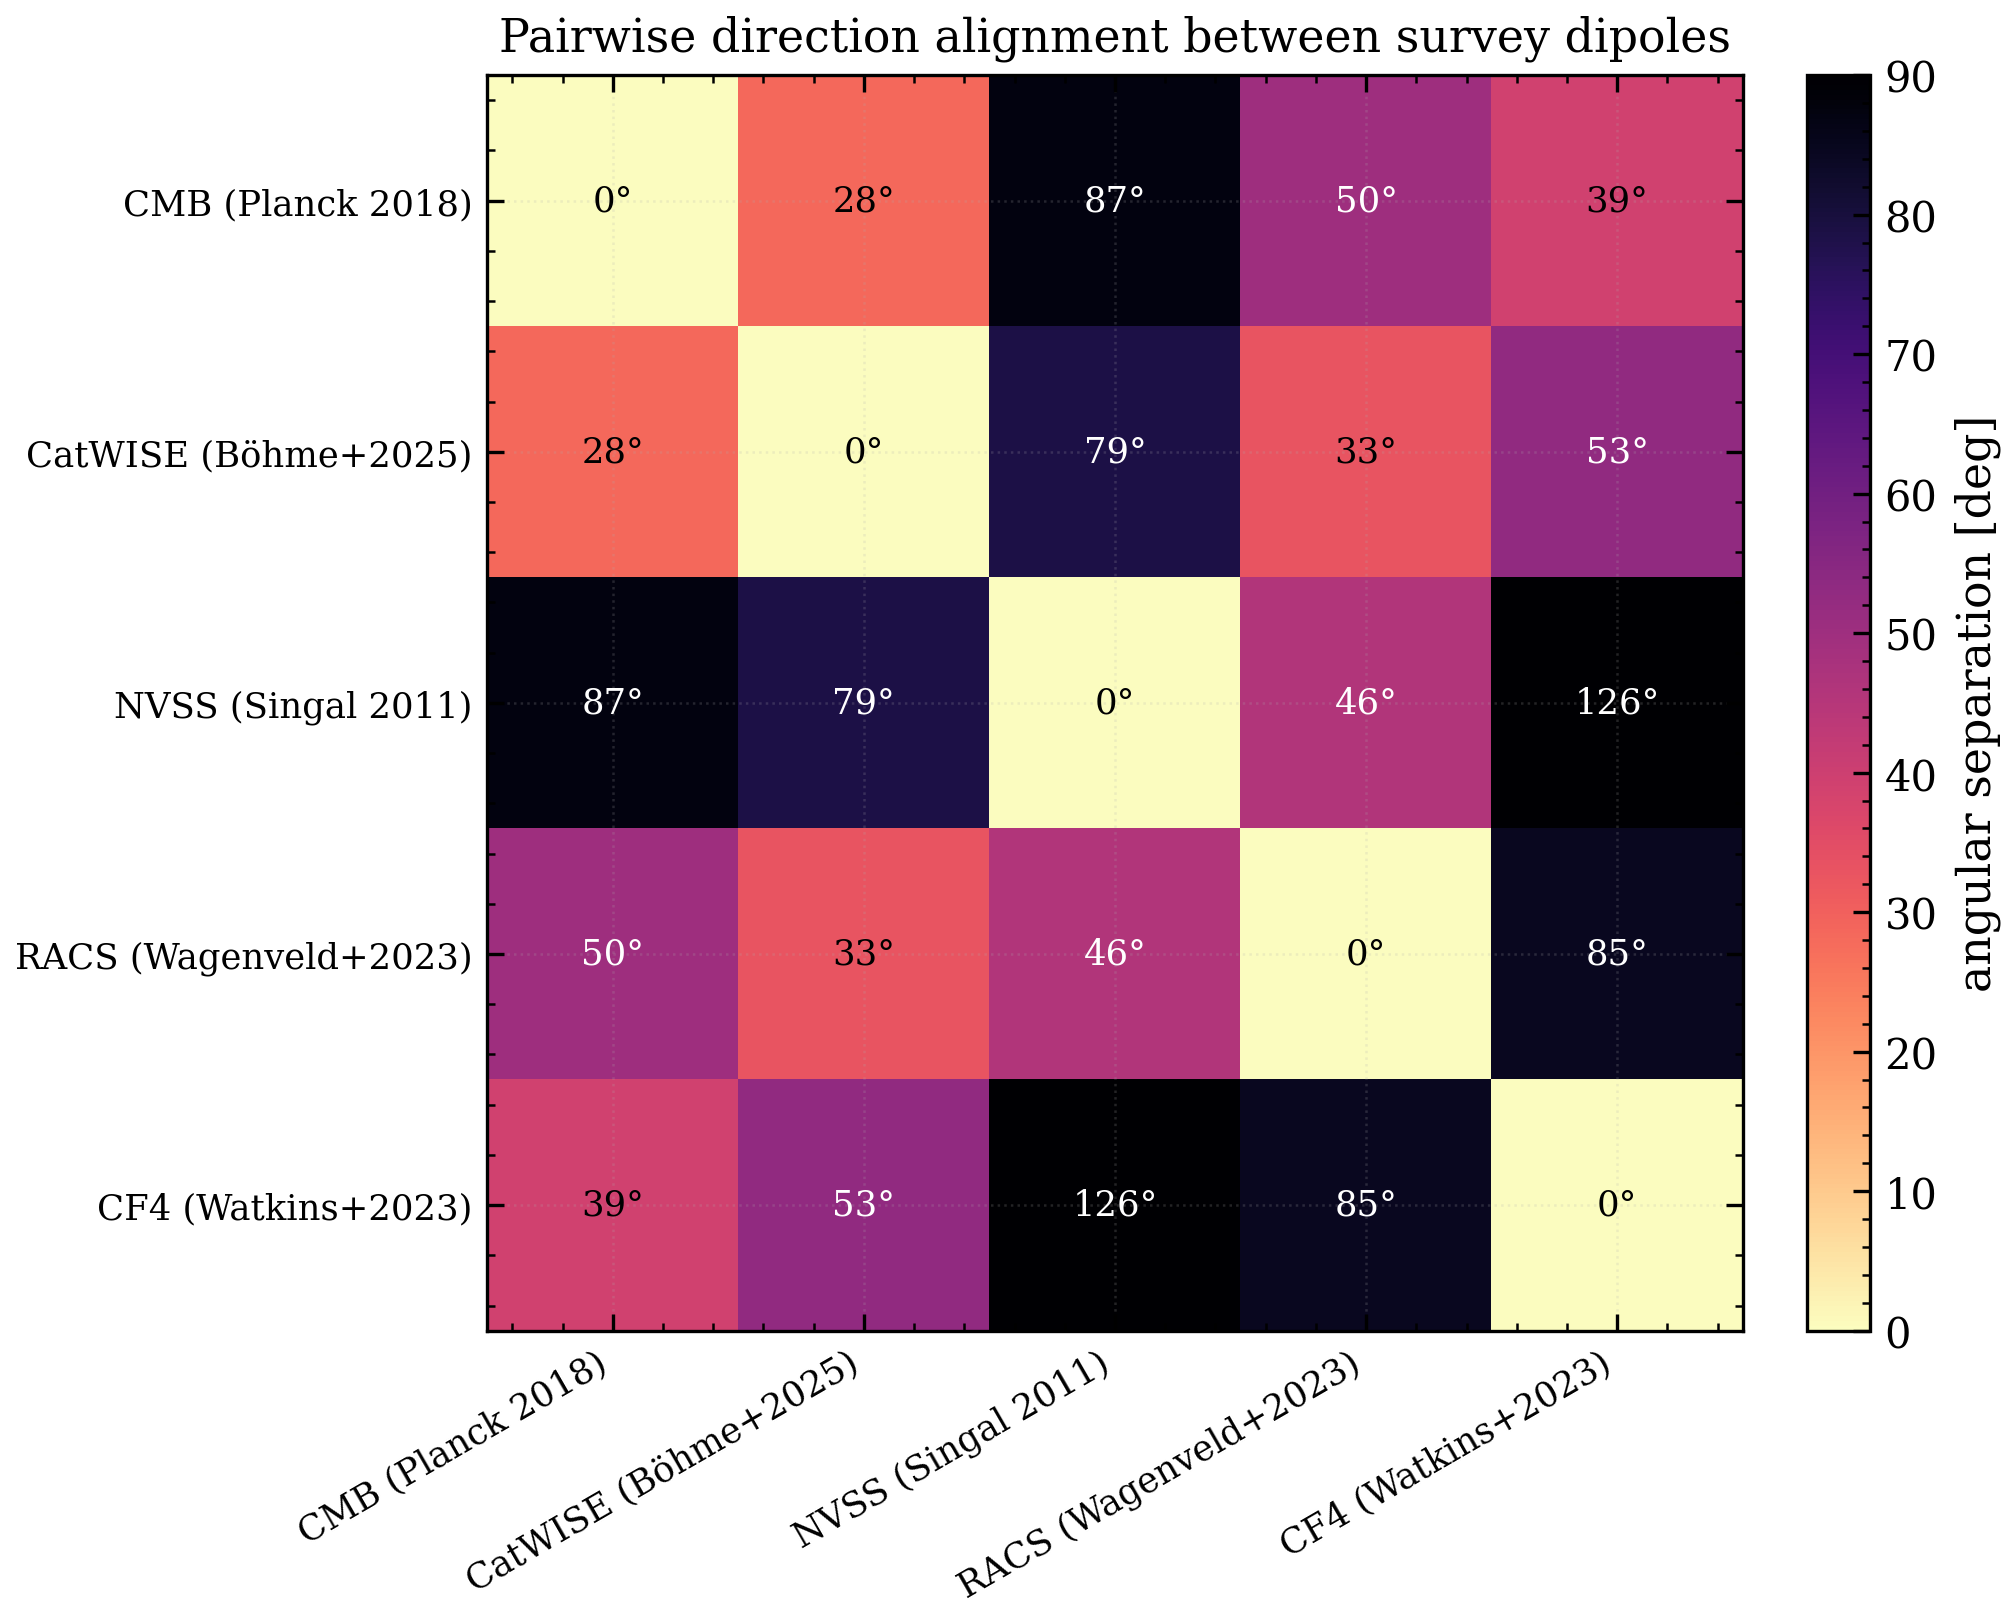
\includegraphics[width=0.82\textwidth,height=0.58\textheight,keepaspectratio]{conditioned_legacy/quarantined-legacy-root-sources__fig_direction_alignment_matrix}
\captionof{figure}{Conditioned legacy diagnostic: direction alignment matrix. Condition: directional artifact with current sky/mask support unresolved. See sidecar manifest for provenance and caveats; appendix-only, not native-transfer or family-ID evidence.}
\label{fig:conditioned-legacy-quarantined-legacy-root-sources-fig-direction-alignment-matrix}
\end{center}

\clearpage
\begin{center}
\centering
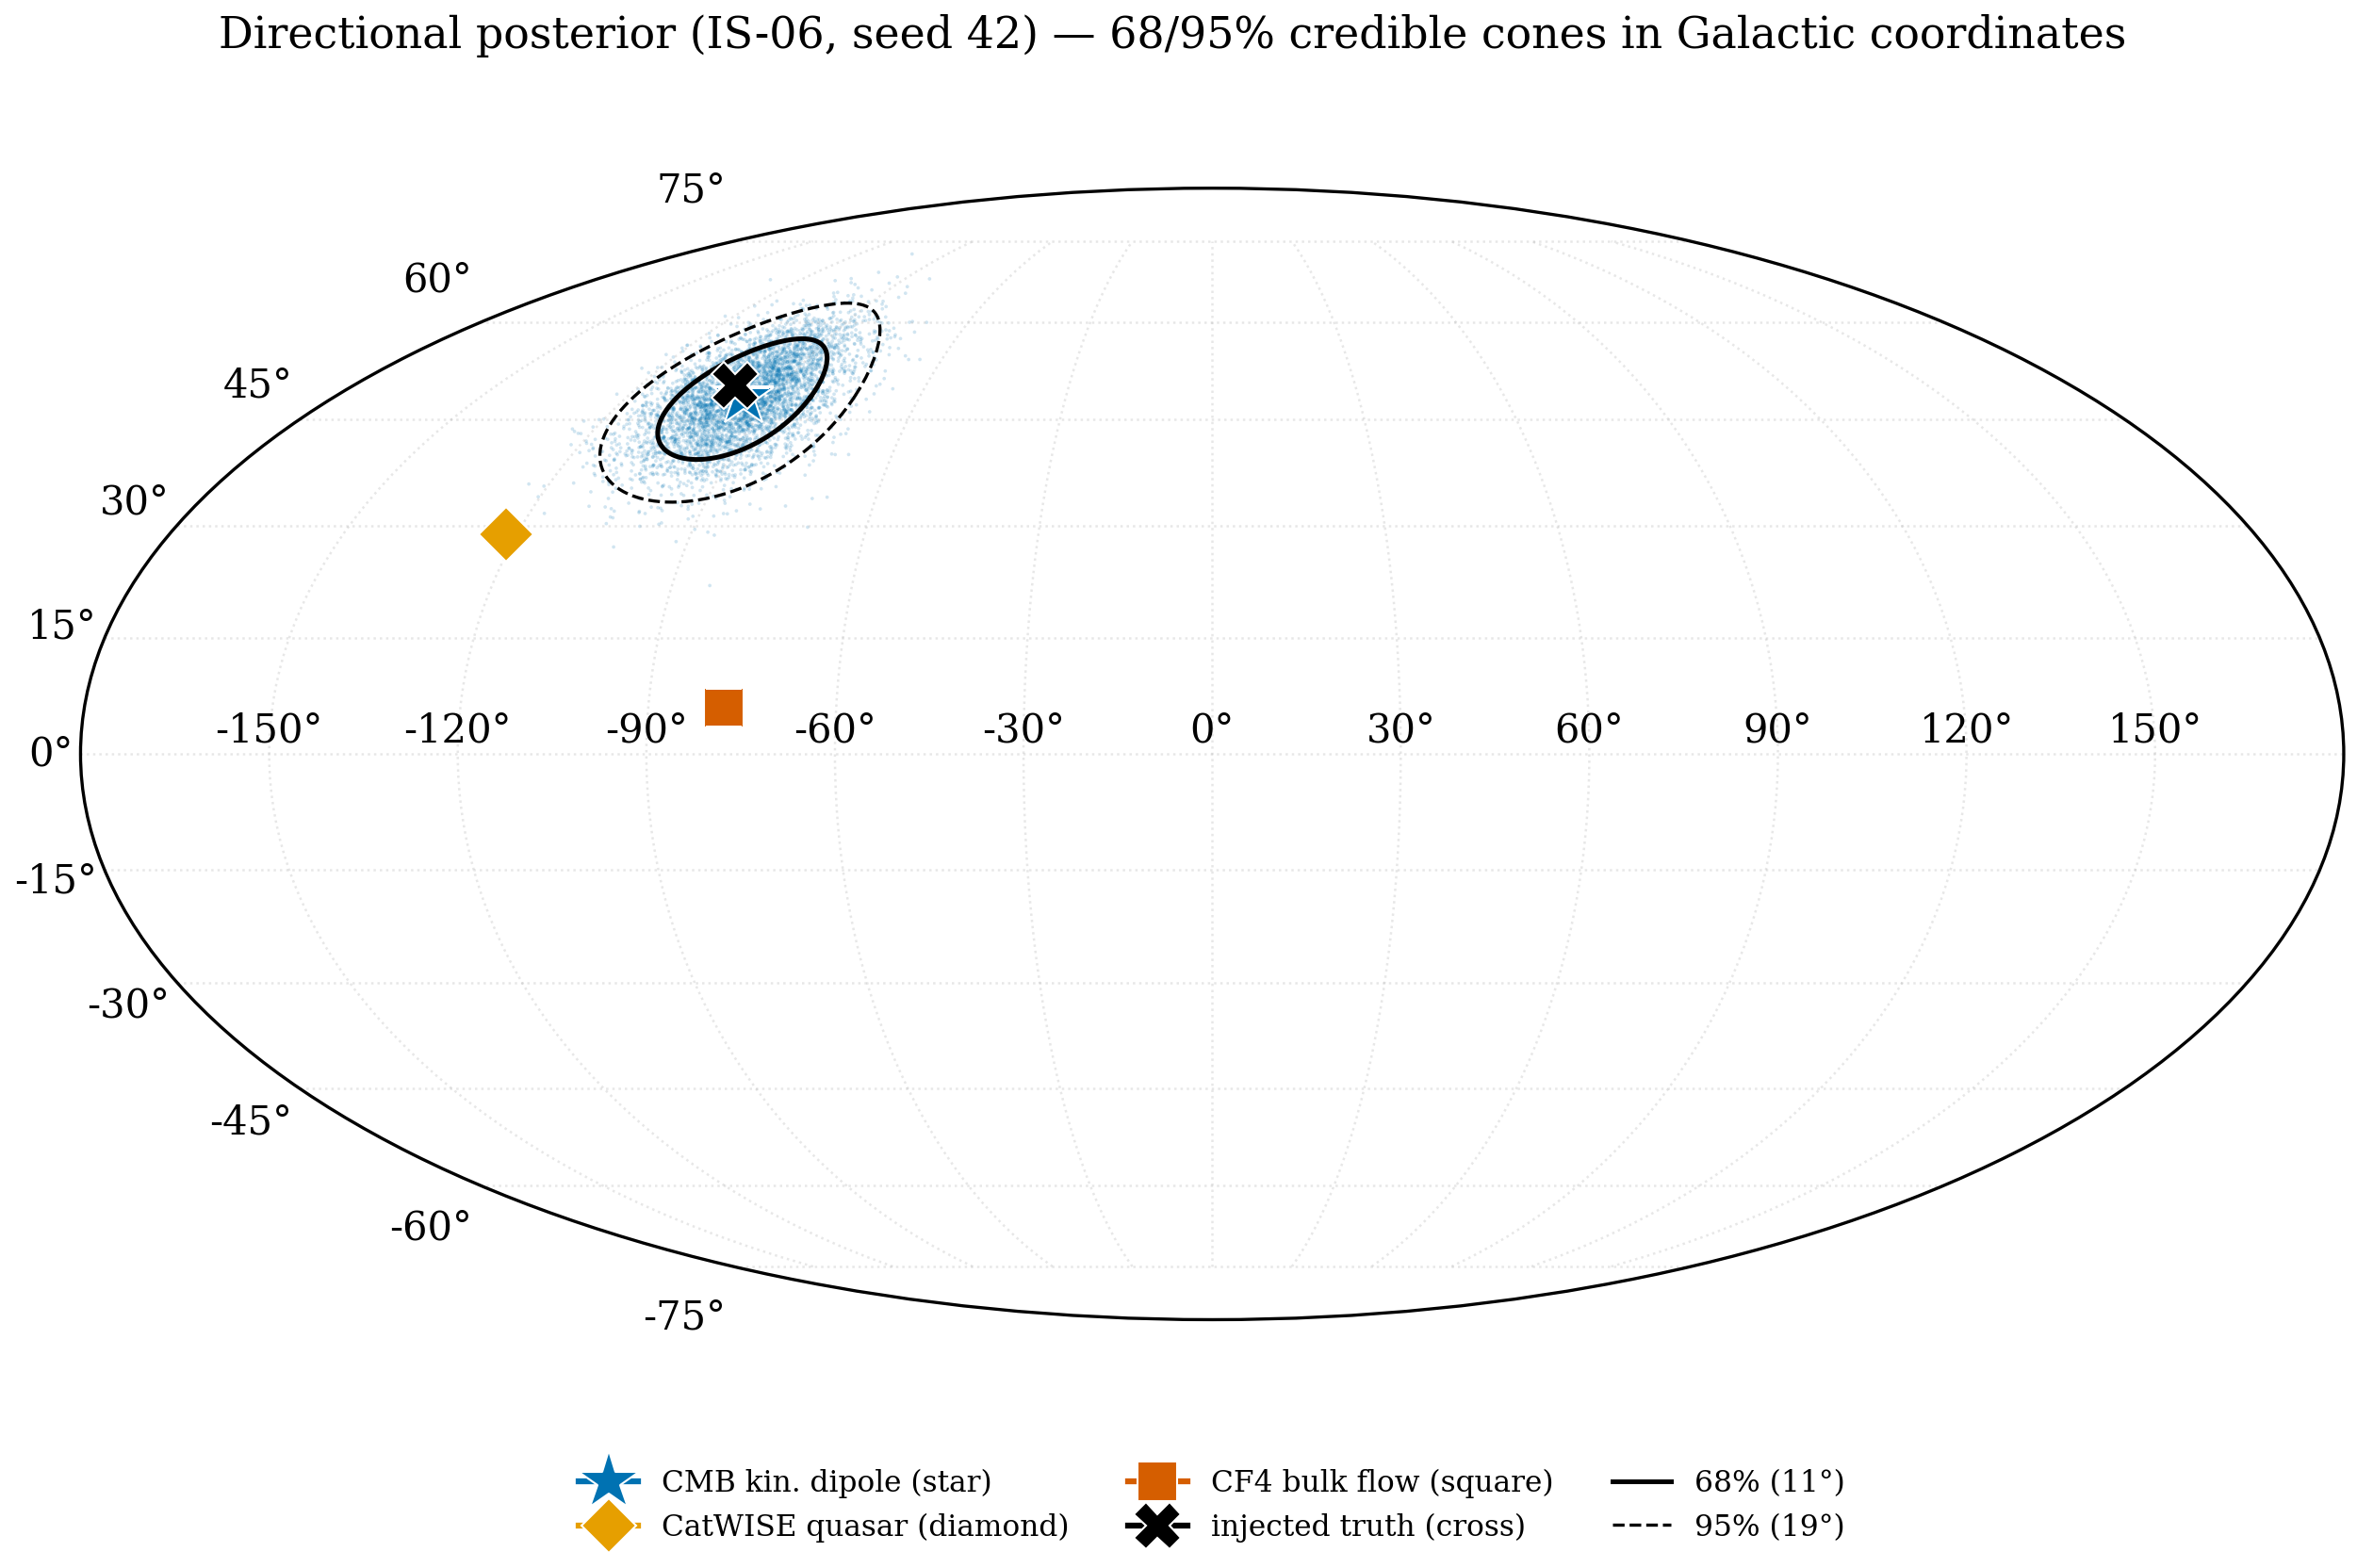
\includegraphics[width=0.82\textwidth,height=0.58\textheight,keepaspectratio]{conditioned_legacy/quarantined-legacy-root-sources__fig_direction_posterior}
\captionof{figure}{Conditioned legacy diagnostic: direction posterior. Condition: legacy statistical assumptions without current null/PPC/LOOCV refresh. See sidecar manifest for provenance and caveats; appendix-only, not native-transfer or family-ID evidence.}
\label{fig:conditioned-legacy-quarantined-legacy-root-sources-fig-direction-posterior}
\end{center}

\clearpage
\begin{center}
\centering
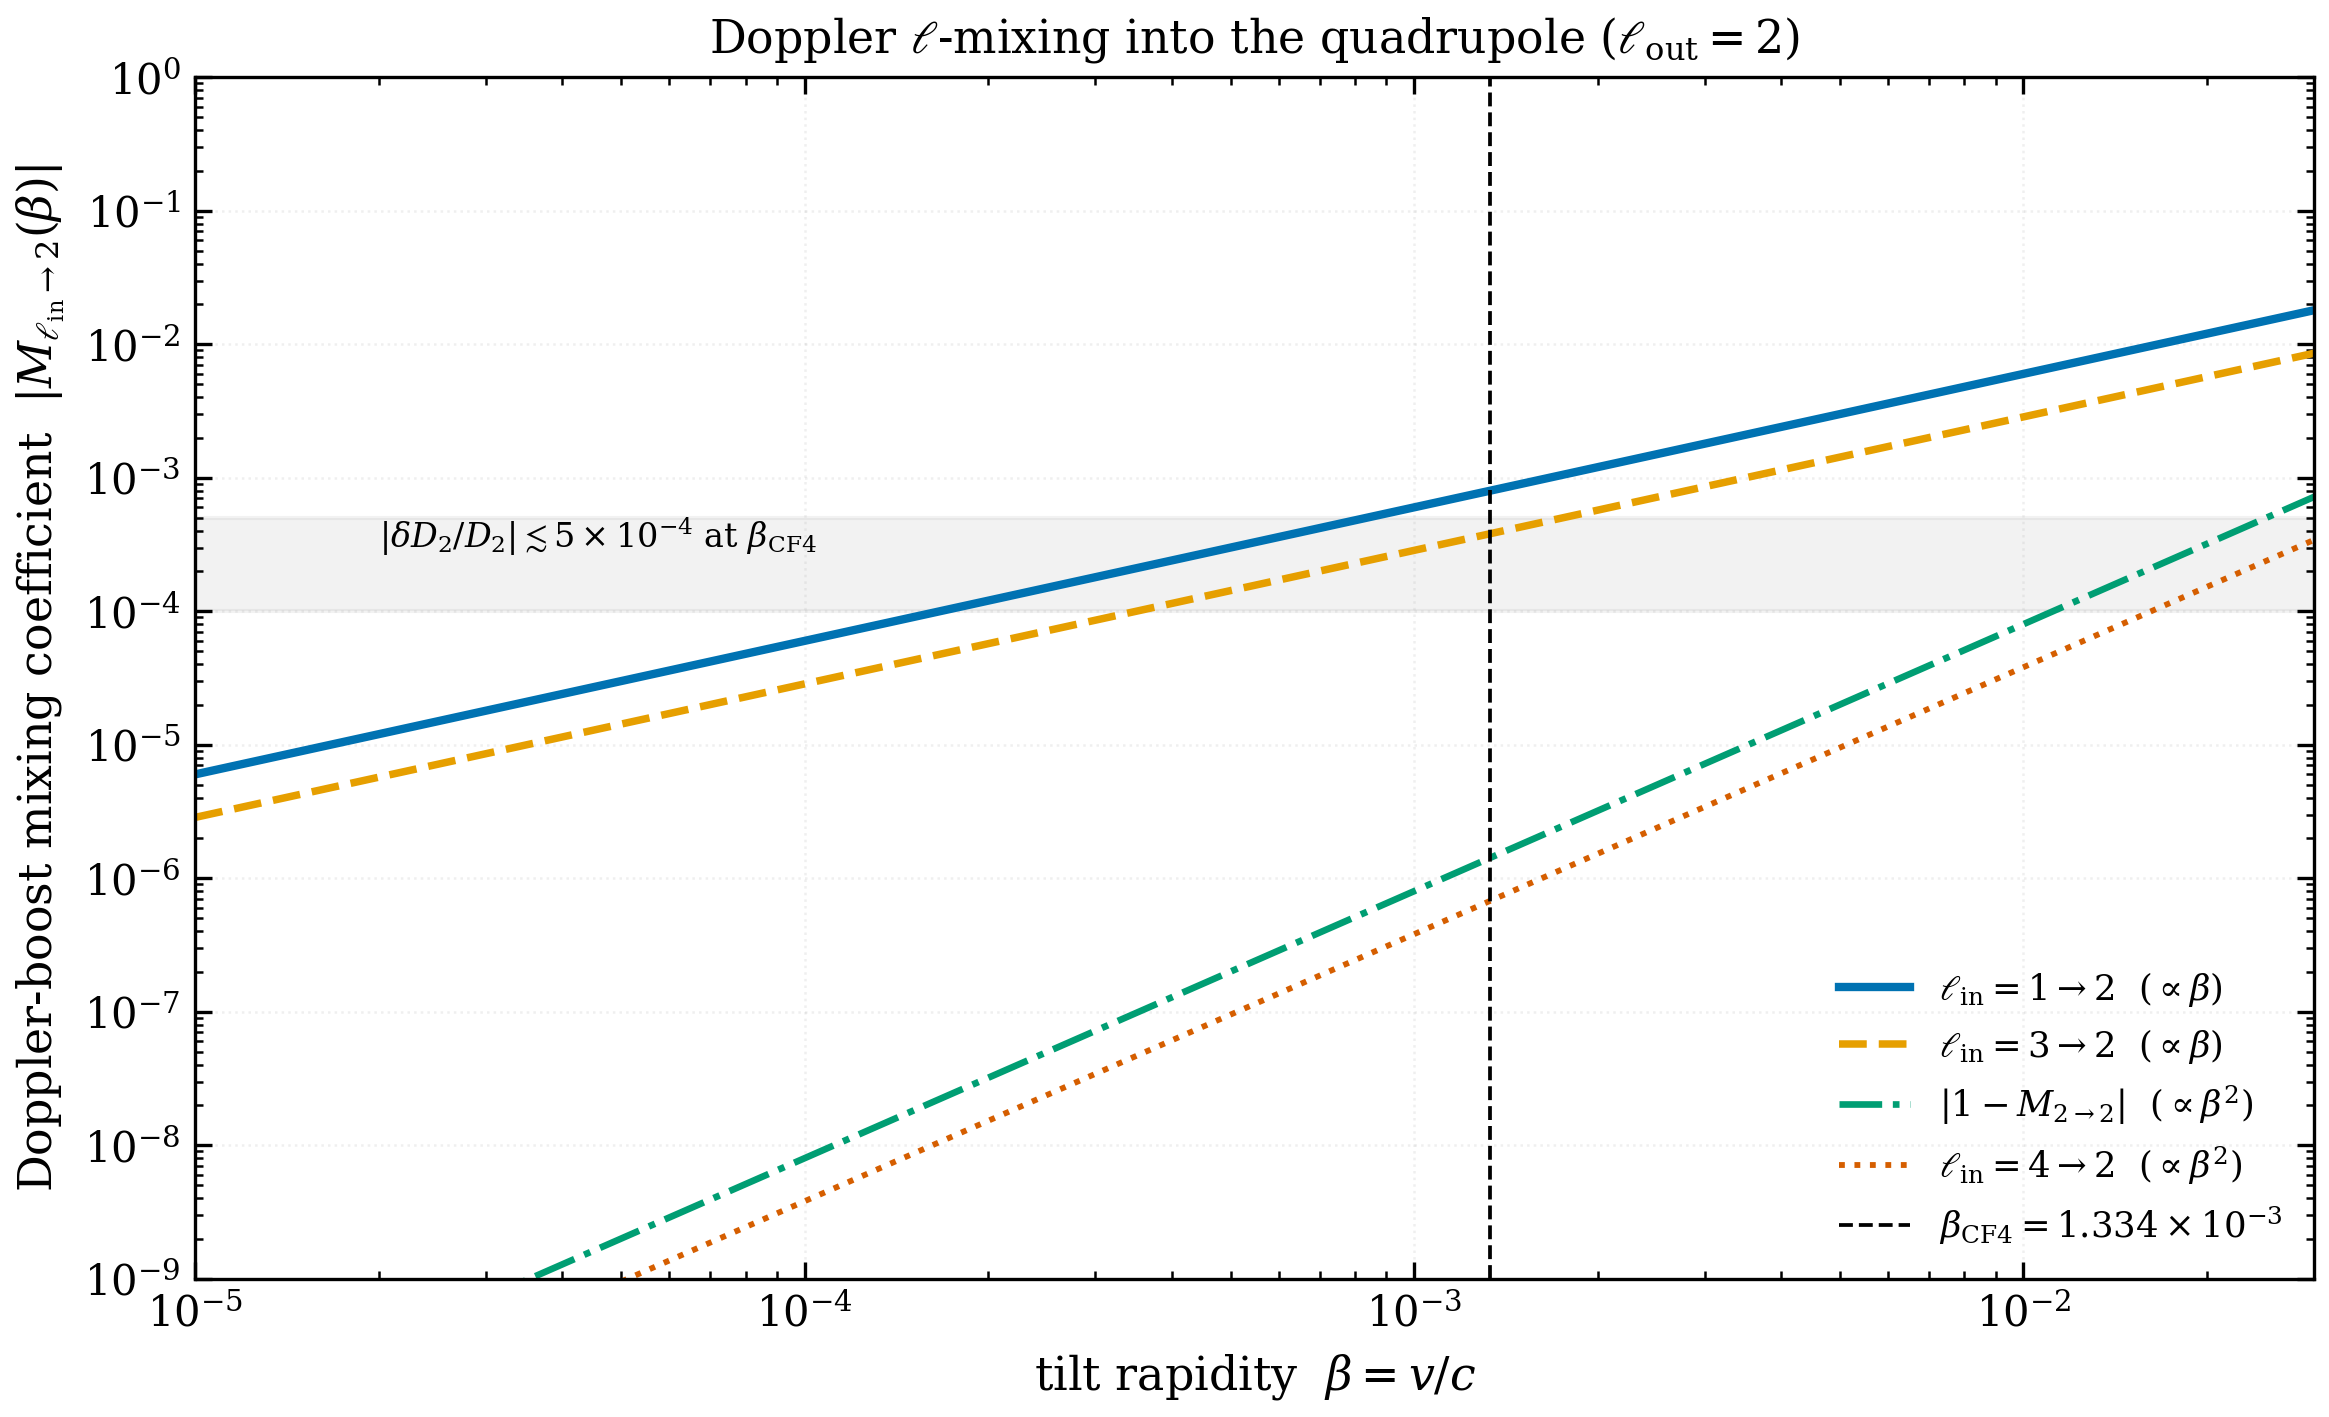
\includegraphics[width=0.82\textwidth,height=0.58\textheight,keepaspectratio]{conditioned_legacy/quarantined-legacy-root-sources__fig_ell_mixing_comparison}
\captionof{figure}{Conditioned legacy diagnostic: ell mixing comparison. Condition: legacy manuscript-generator assumptions. See sidecar manifest for provenance and caveats; appendix-only, not native-transfer or family-ID evidence.}
\label{fig:conditioned-legacy-quarantined-legacy-root-sources-fig-ell-mixing-comparison}
\end{center}

\clearpage
\begin{center}
\centering
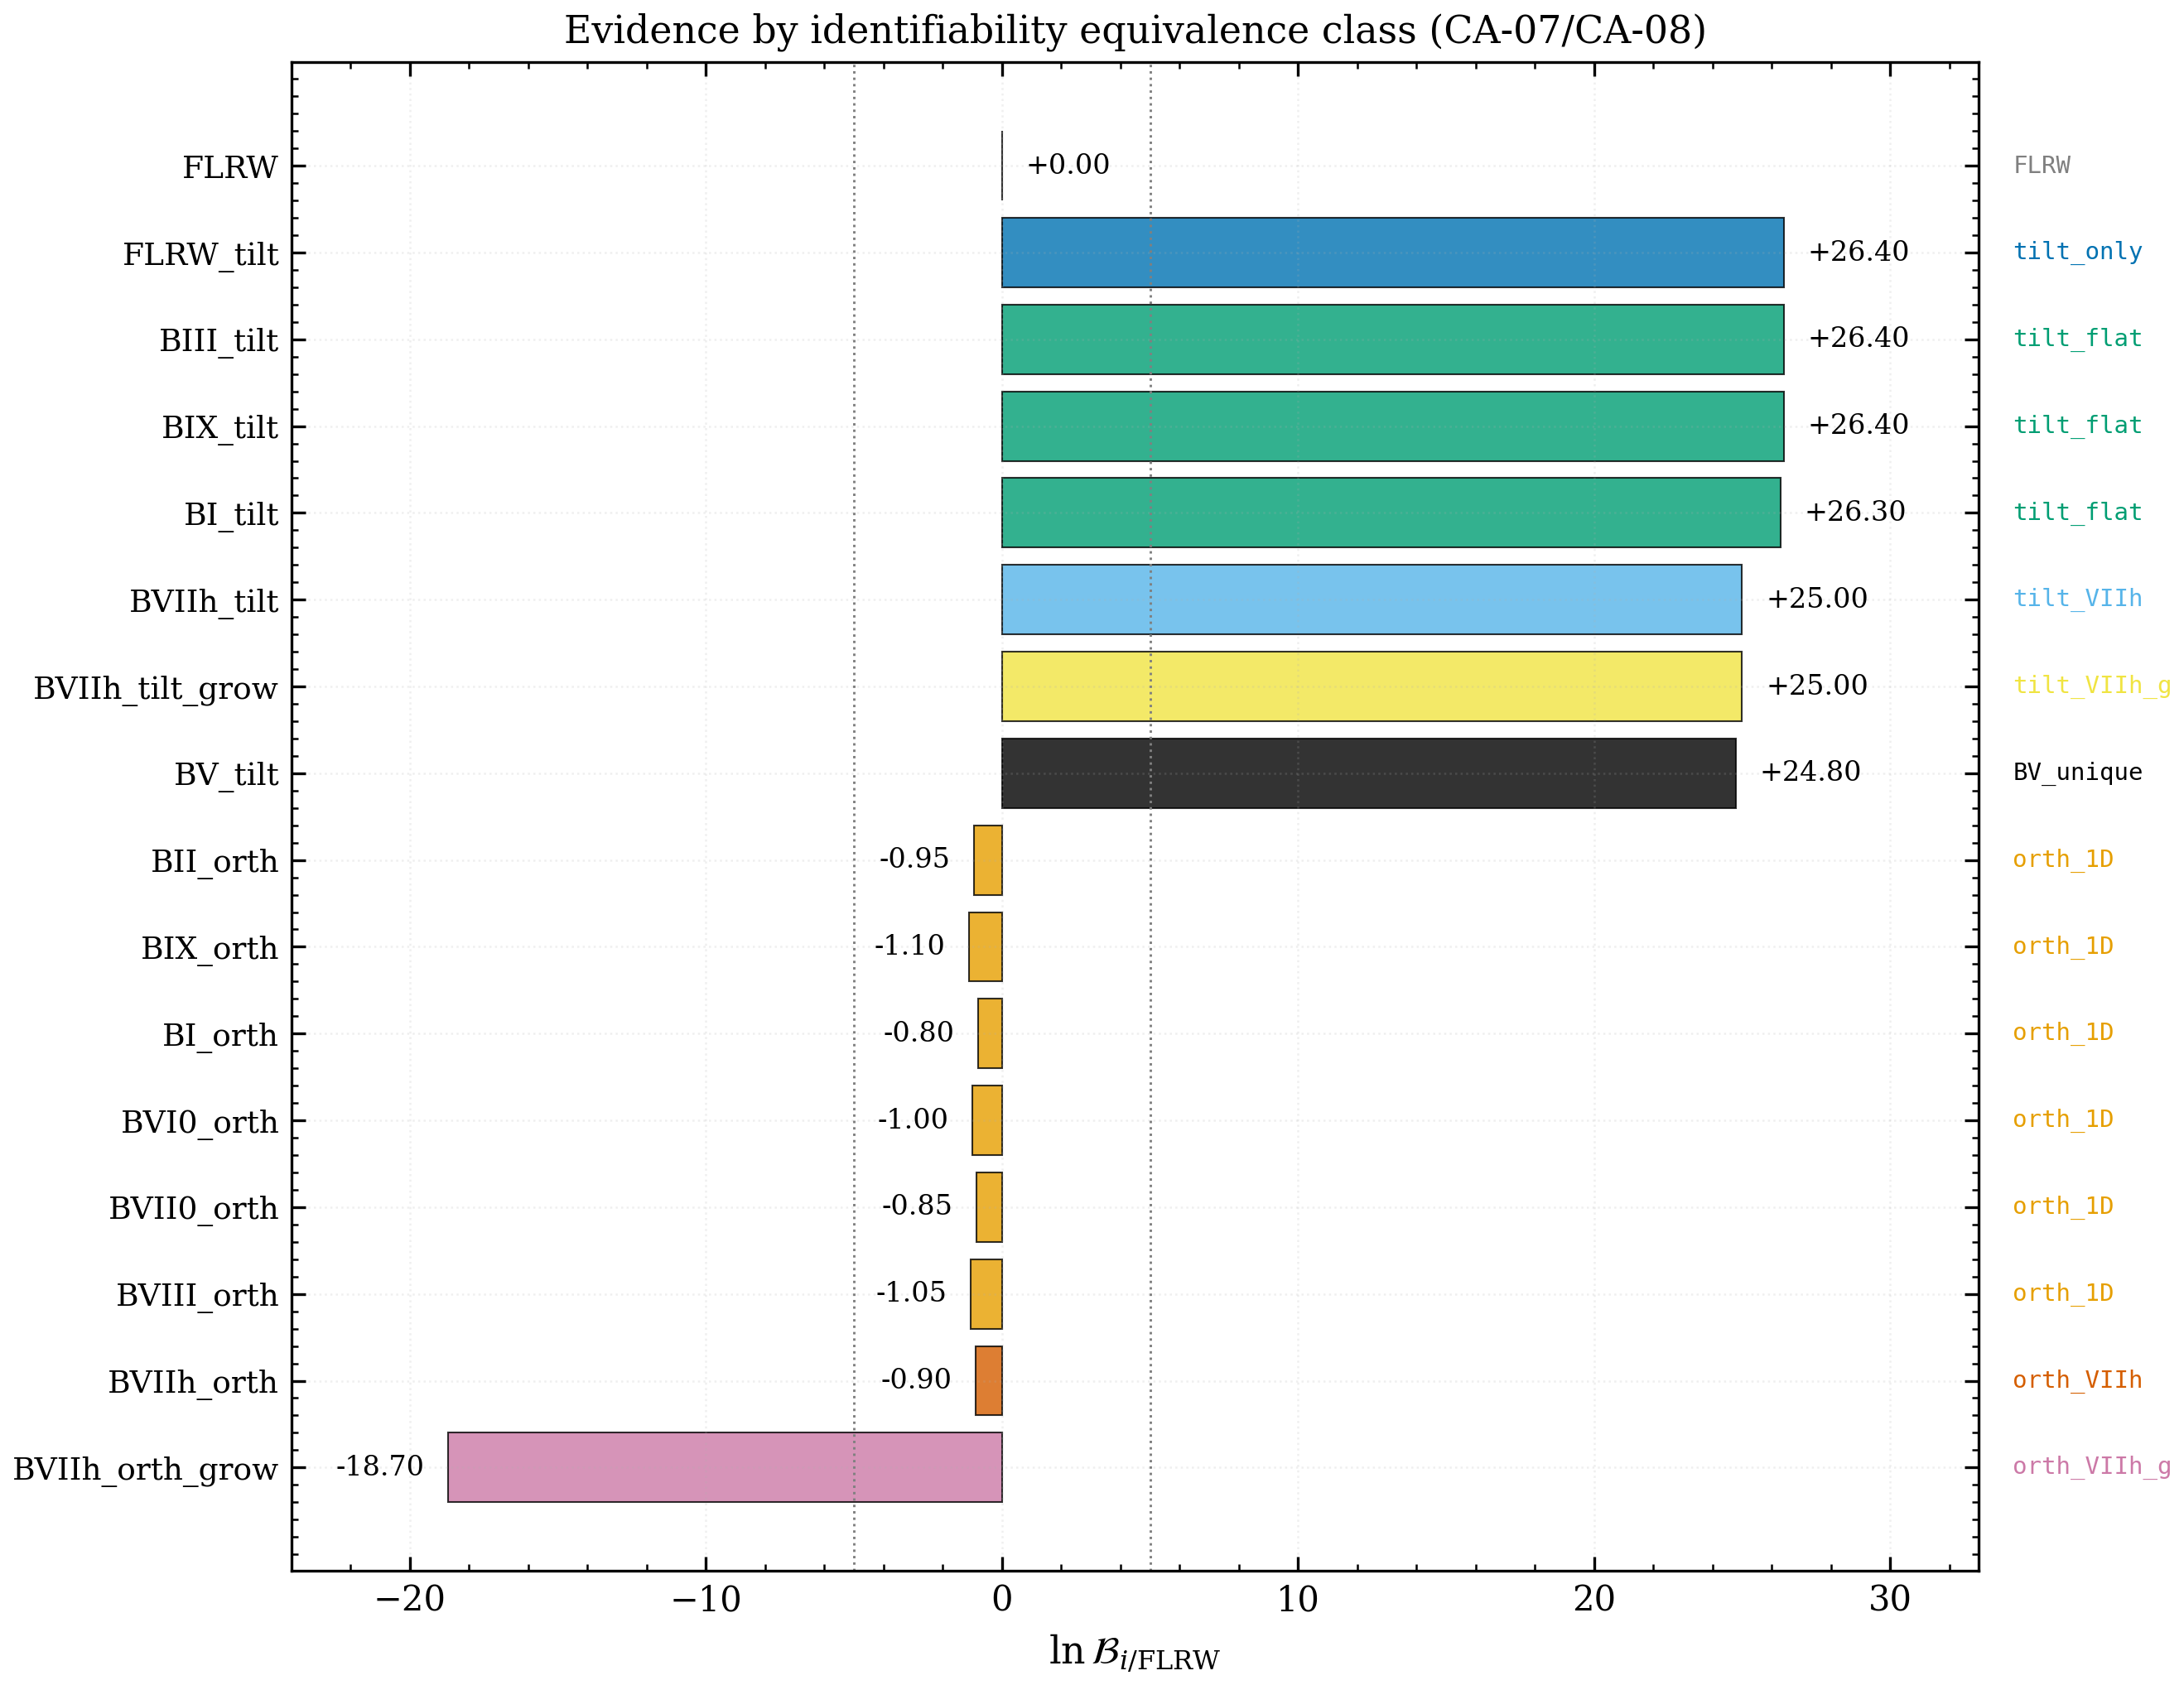
\includegraphics[width=0.82\textwidth,height=0.58\textheight,keepaspectratio]{conditioned_legacy/quarantined-legacy-root-sources__fig_equiv_class_evidence}
\captionof{figure}{Conditioned legacy diagnostic: equiv class evidence. Condition: legacy statistical assumptions without current null/PPC/LOOCV refresh. See sidecar manifest for provenance and caveats; appendix-only, not native-transfer or family-ID evidence.}
\label{fig:conditioned-legacy-quarantined-legacy-root-sources-fig-equiv-class-evidence}
\end{center}

\clearpage
\begin{center}
\centering
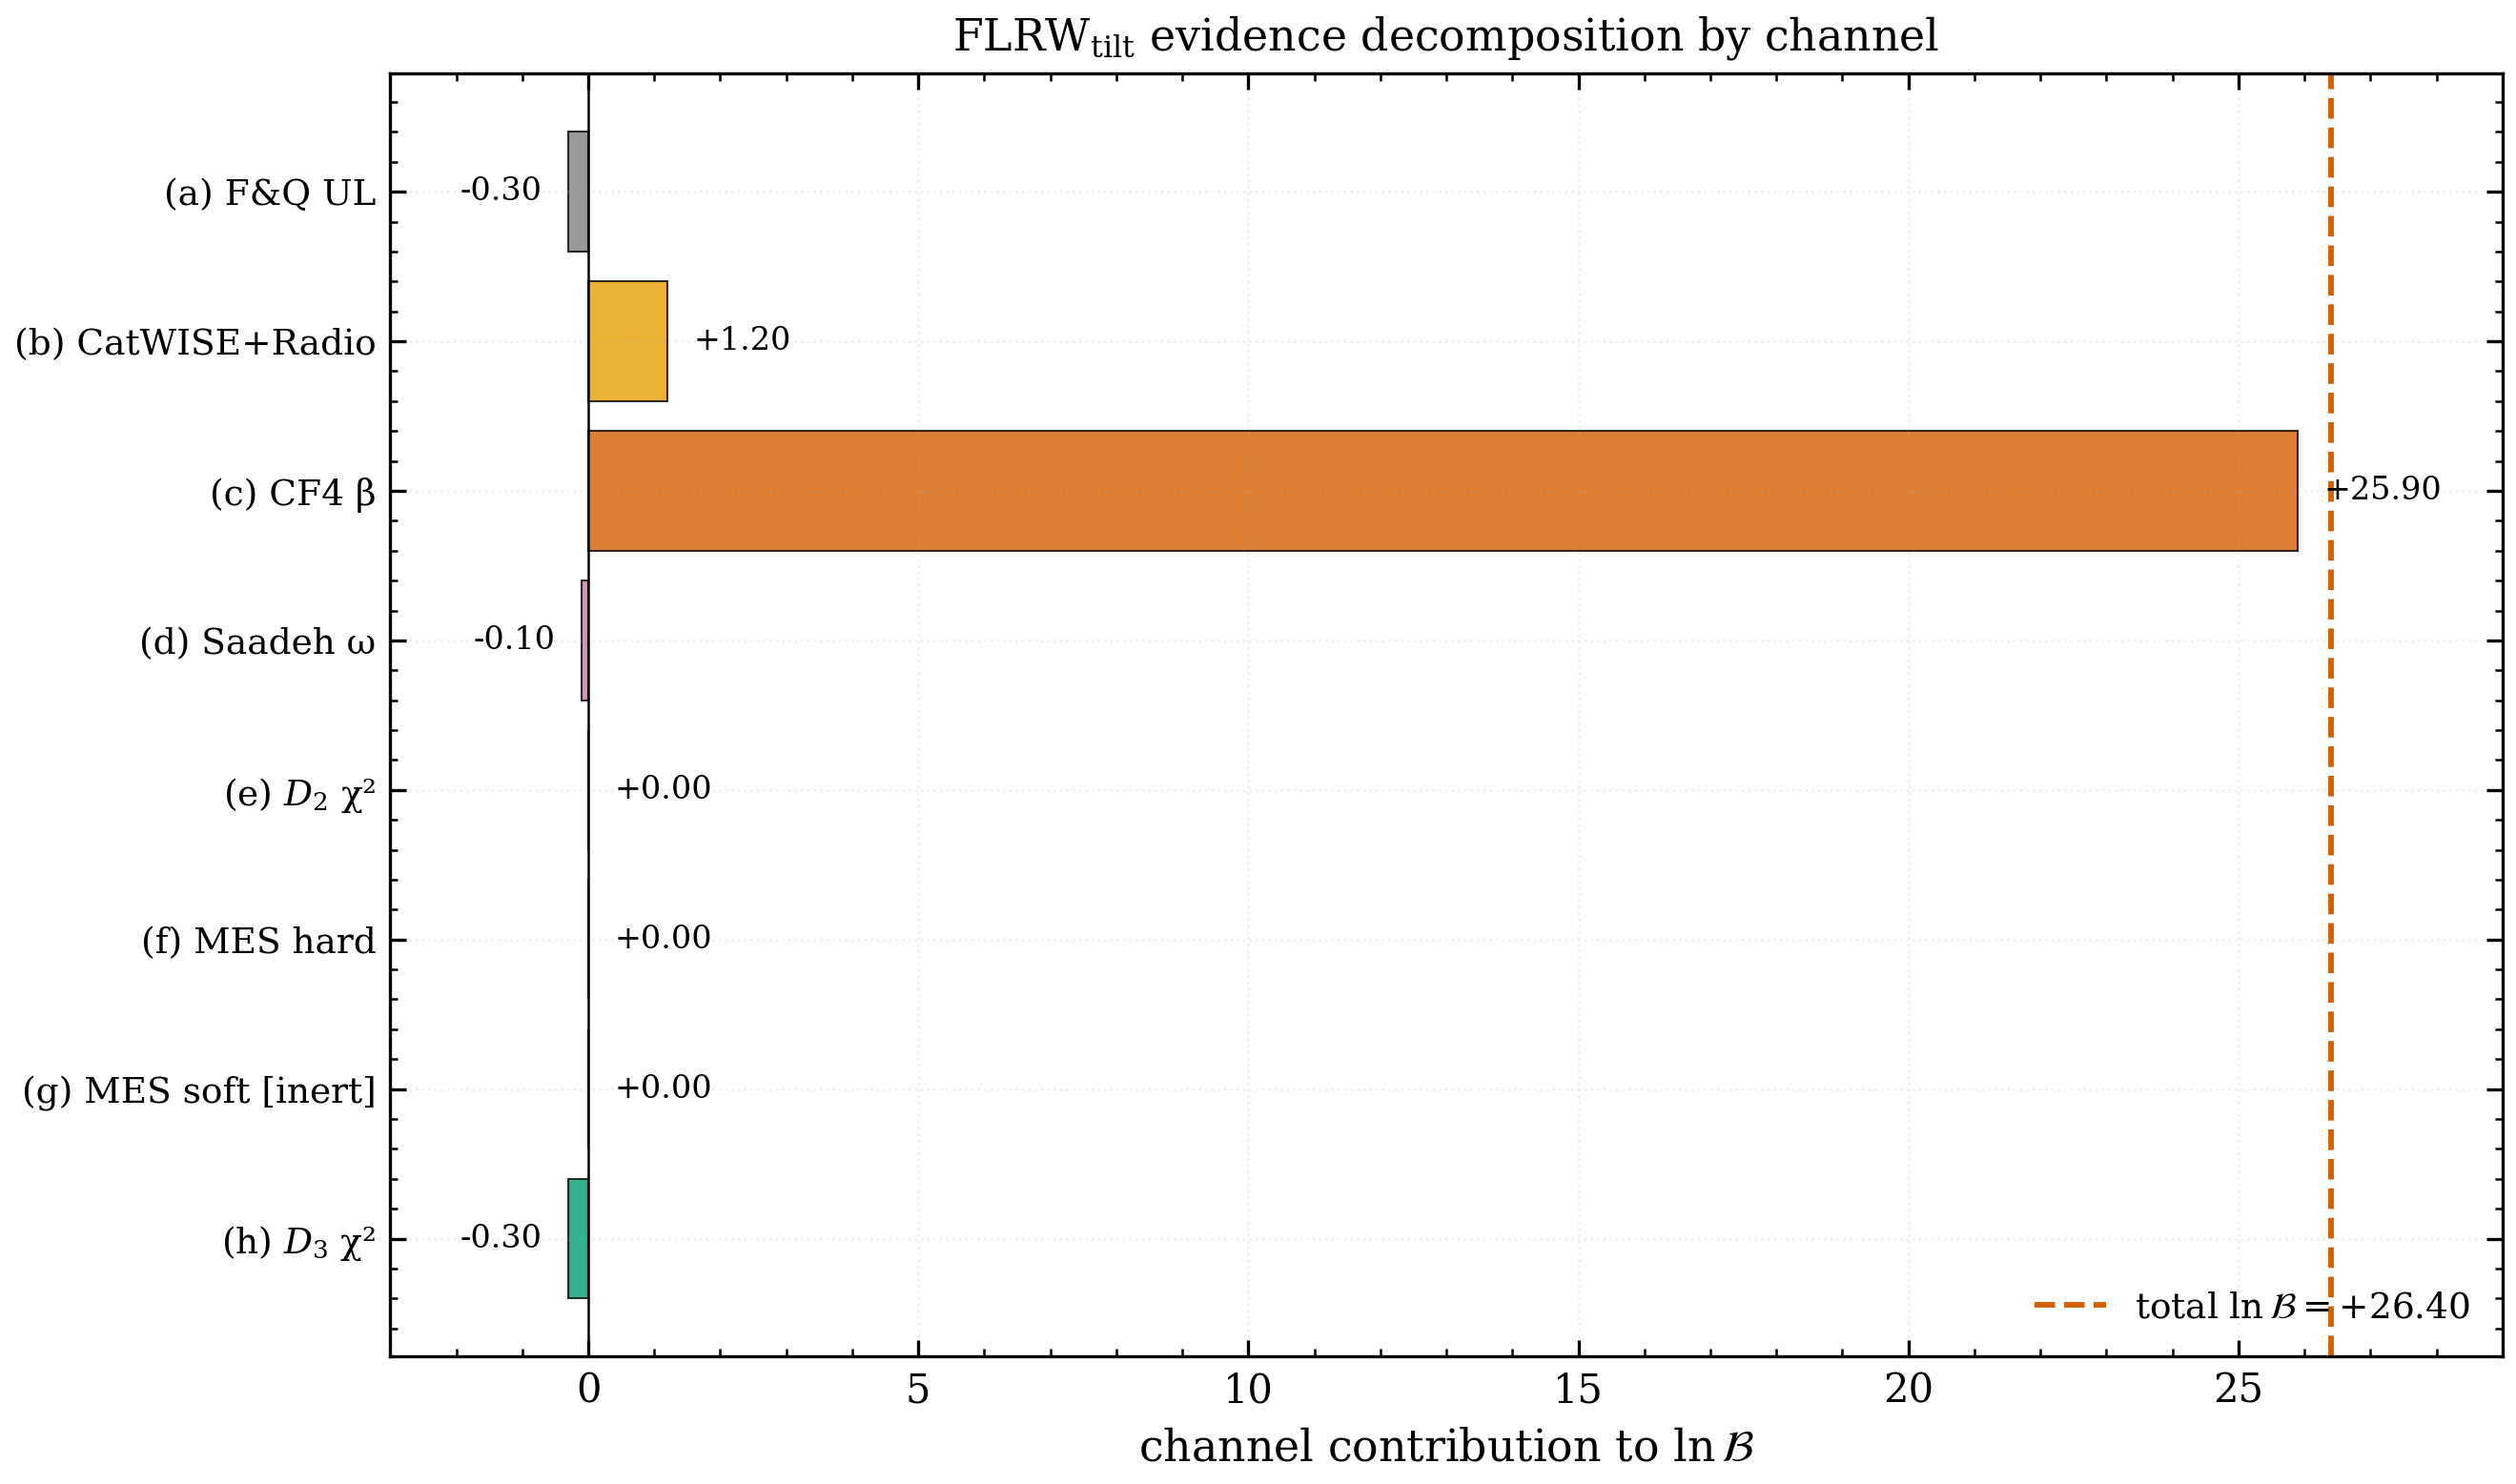
\includegraphics[width=0.82\textwidth,height=0.58\textheight,keepaspectratio]{conditioned_legacy/quarantined-legacy-root-sources__fig_evidence_decomposition}
\captionof{figure}{Conditioned legacy diagnostic: evidence decomposition. Condition: legacy statistical assumptions without current null/PPC/LOOCV refresh. See sidecar manifest for provenance and caveats; appendix-only, not native-transfer or family-ID evidence.}
\label{fig:conditioned-legacy-quarantined-legacy-root-sources-fig-evidence-decomposition}
\end{center}

\clearpage
\begin{center}
\centering
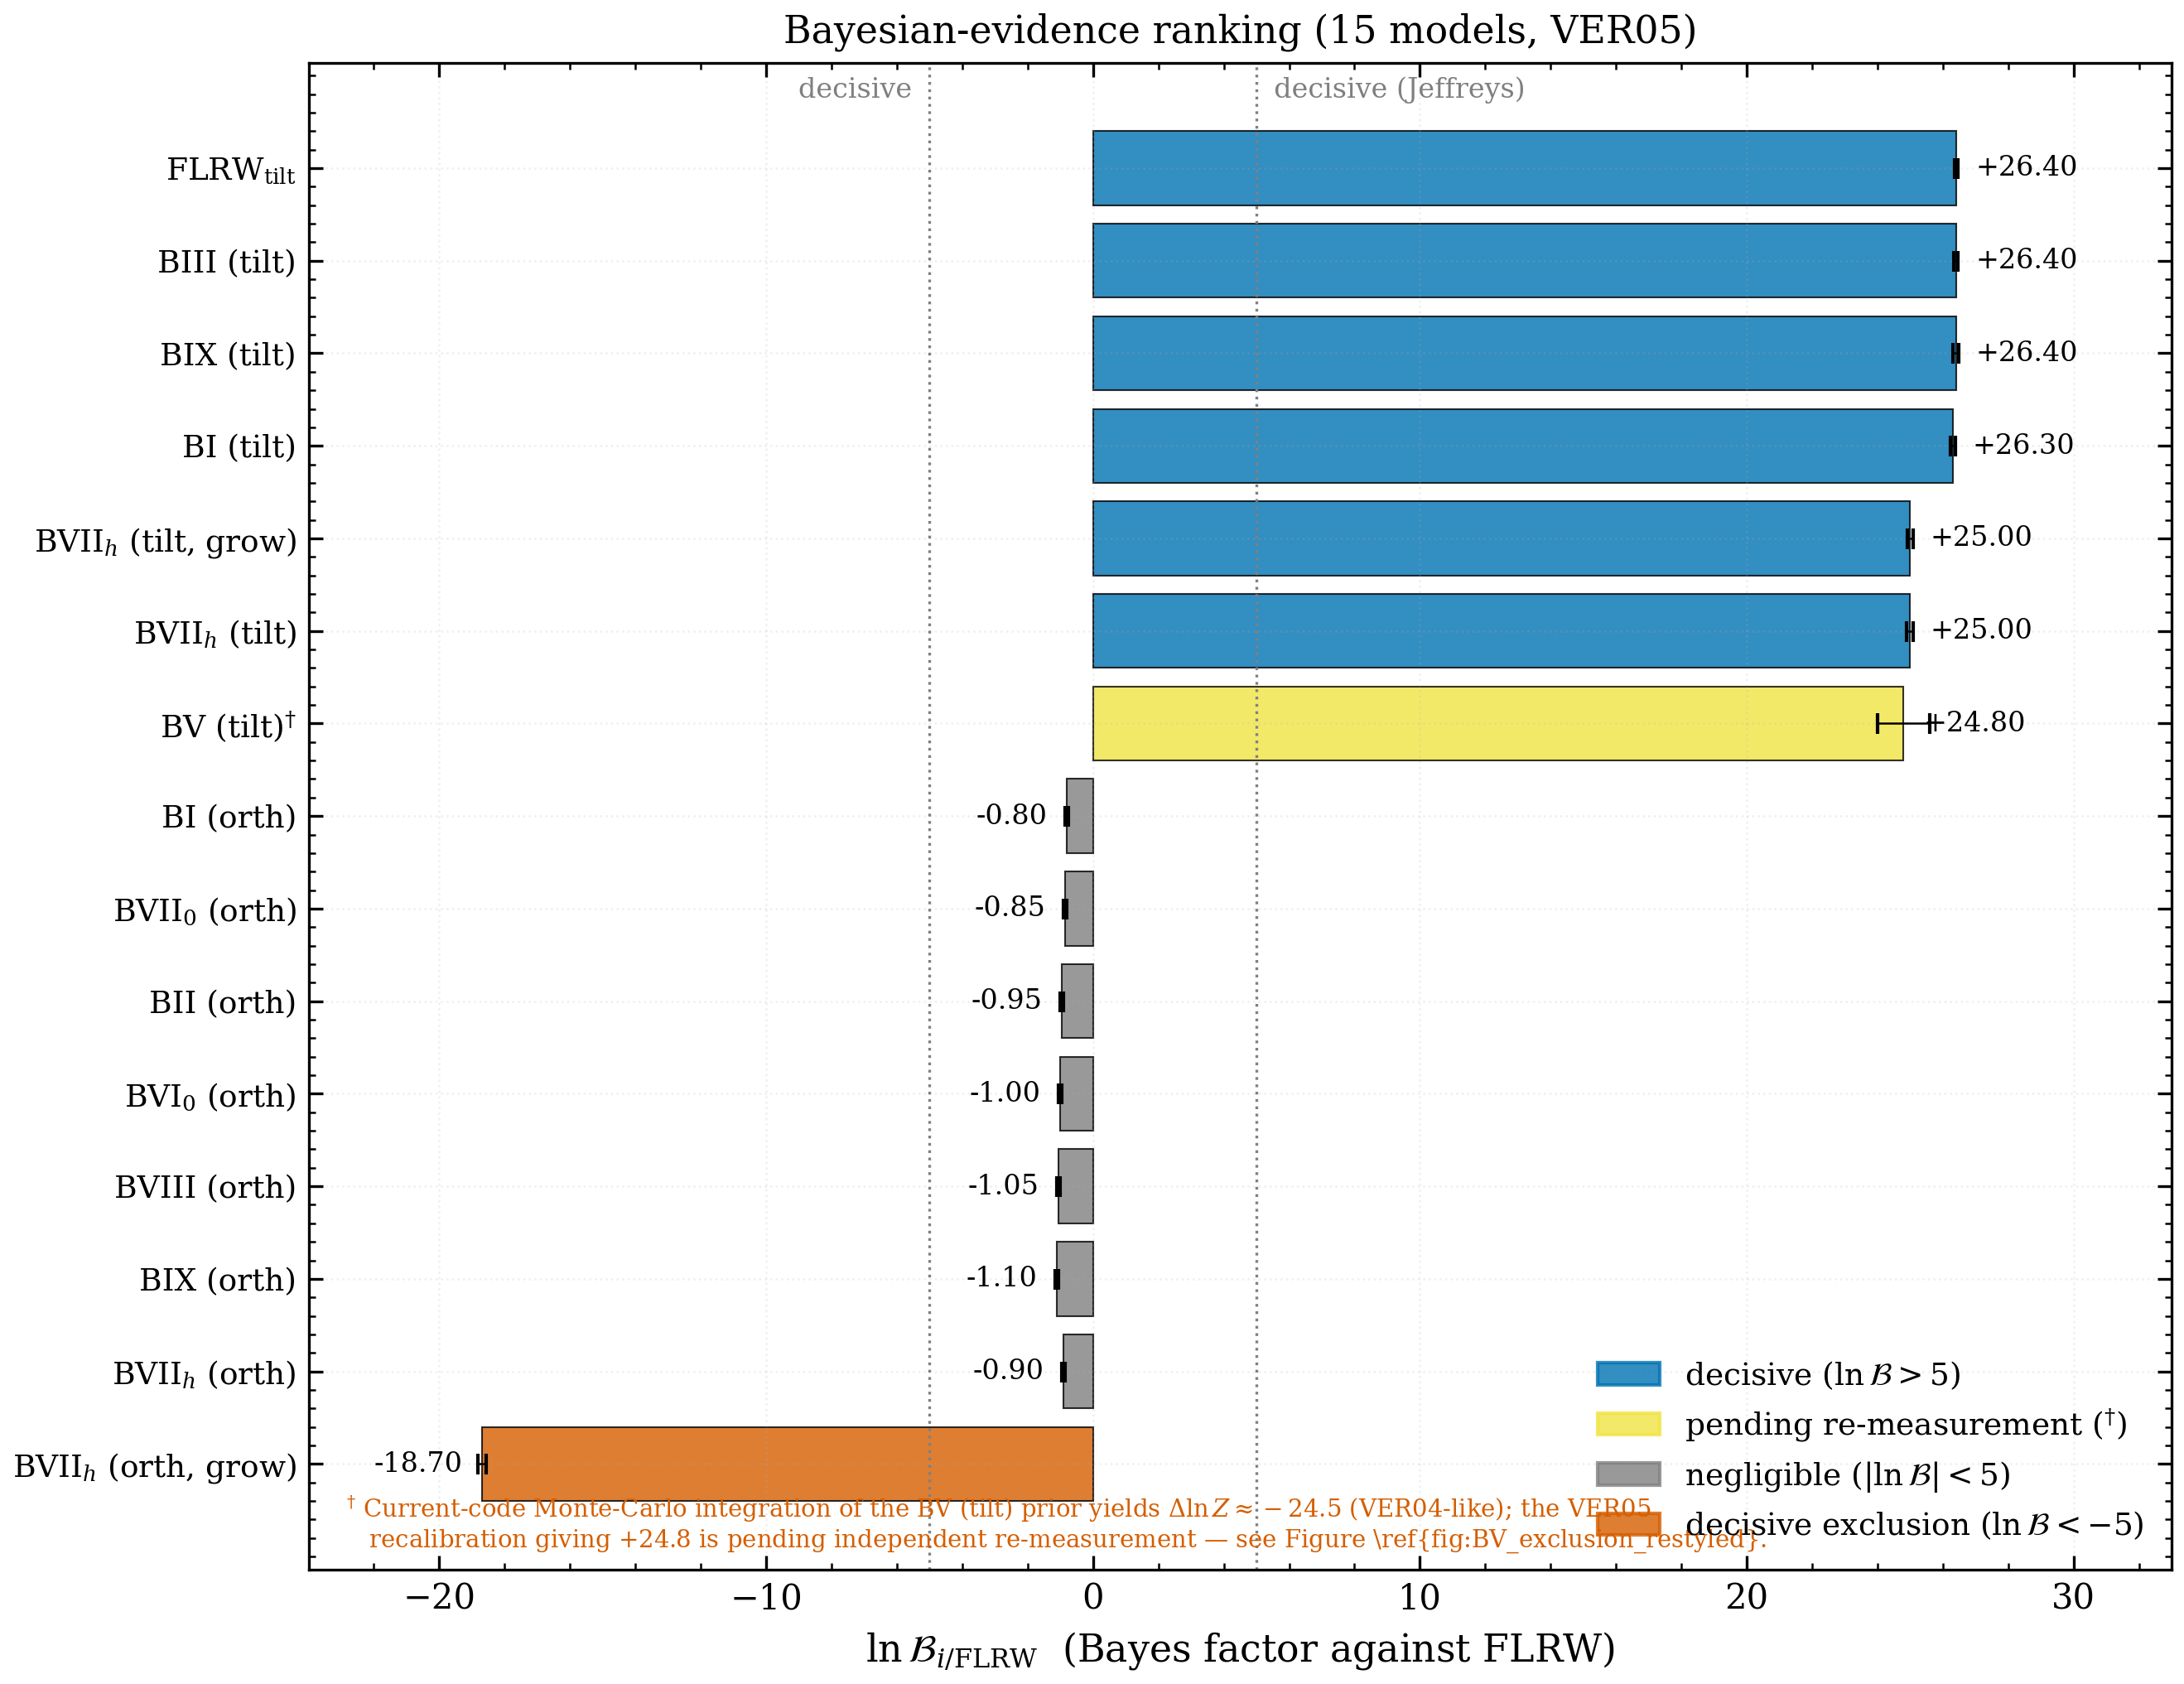
\includegraphics[width=0.82\textwidth,height=0.58\textheight,keepaspectratio]{conditioned_legacy/quarantined-legacy-root-sources__fig_evidence_grand_bar}
\captionof{figure}{Conditioned legacy diagnostic: evidence grand bar. Condition: legacy statistical assumptions without current null/PPC/LOOCV refresh. See sidecar manifest for provenance and caveats; appendix-only, not native-transfer or family-ID evidence.}
\label{fig:conditioned-legacy-quarantined-legacy-root-sources-fig-evidence-grand-bar}
\end{center}

\clearpage
\begin{center}
\centering
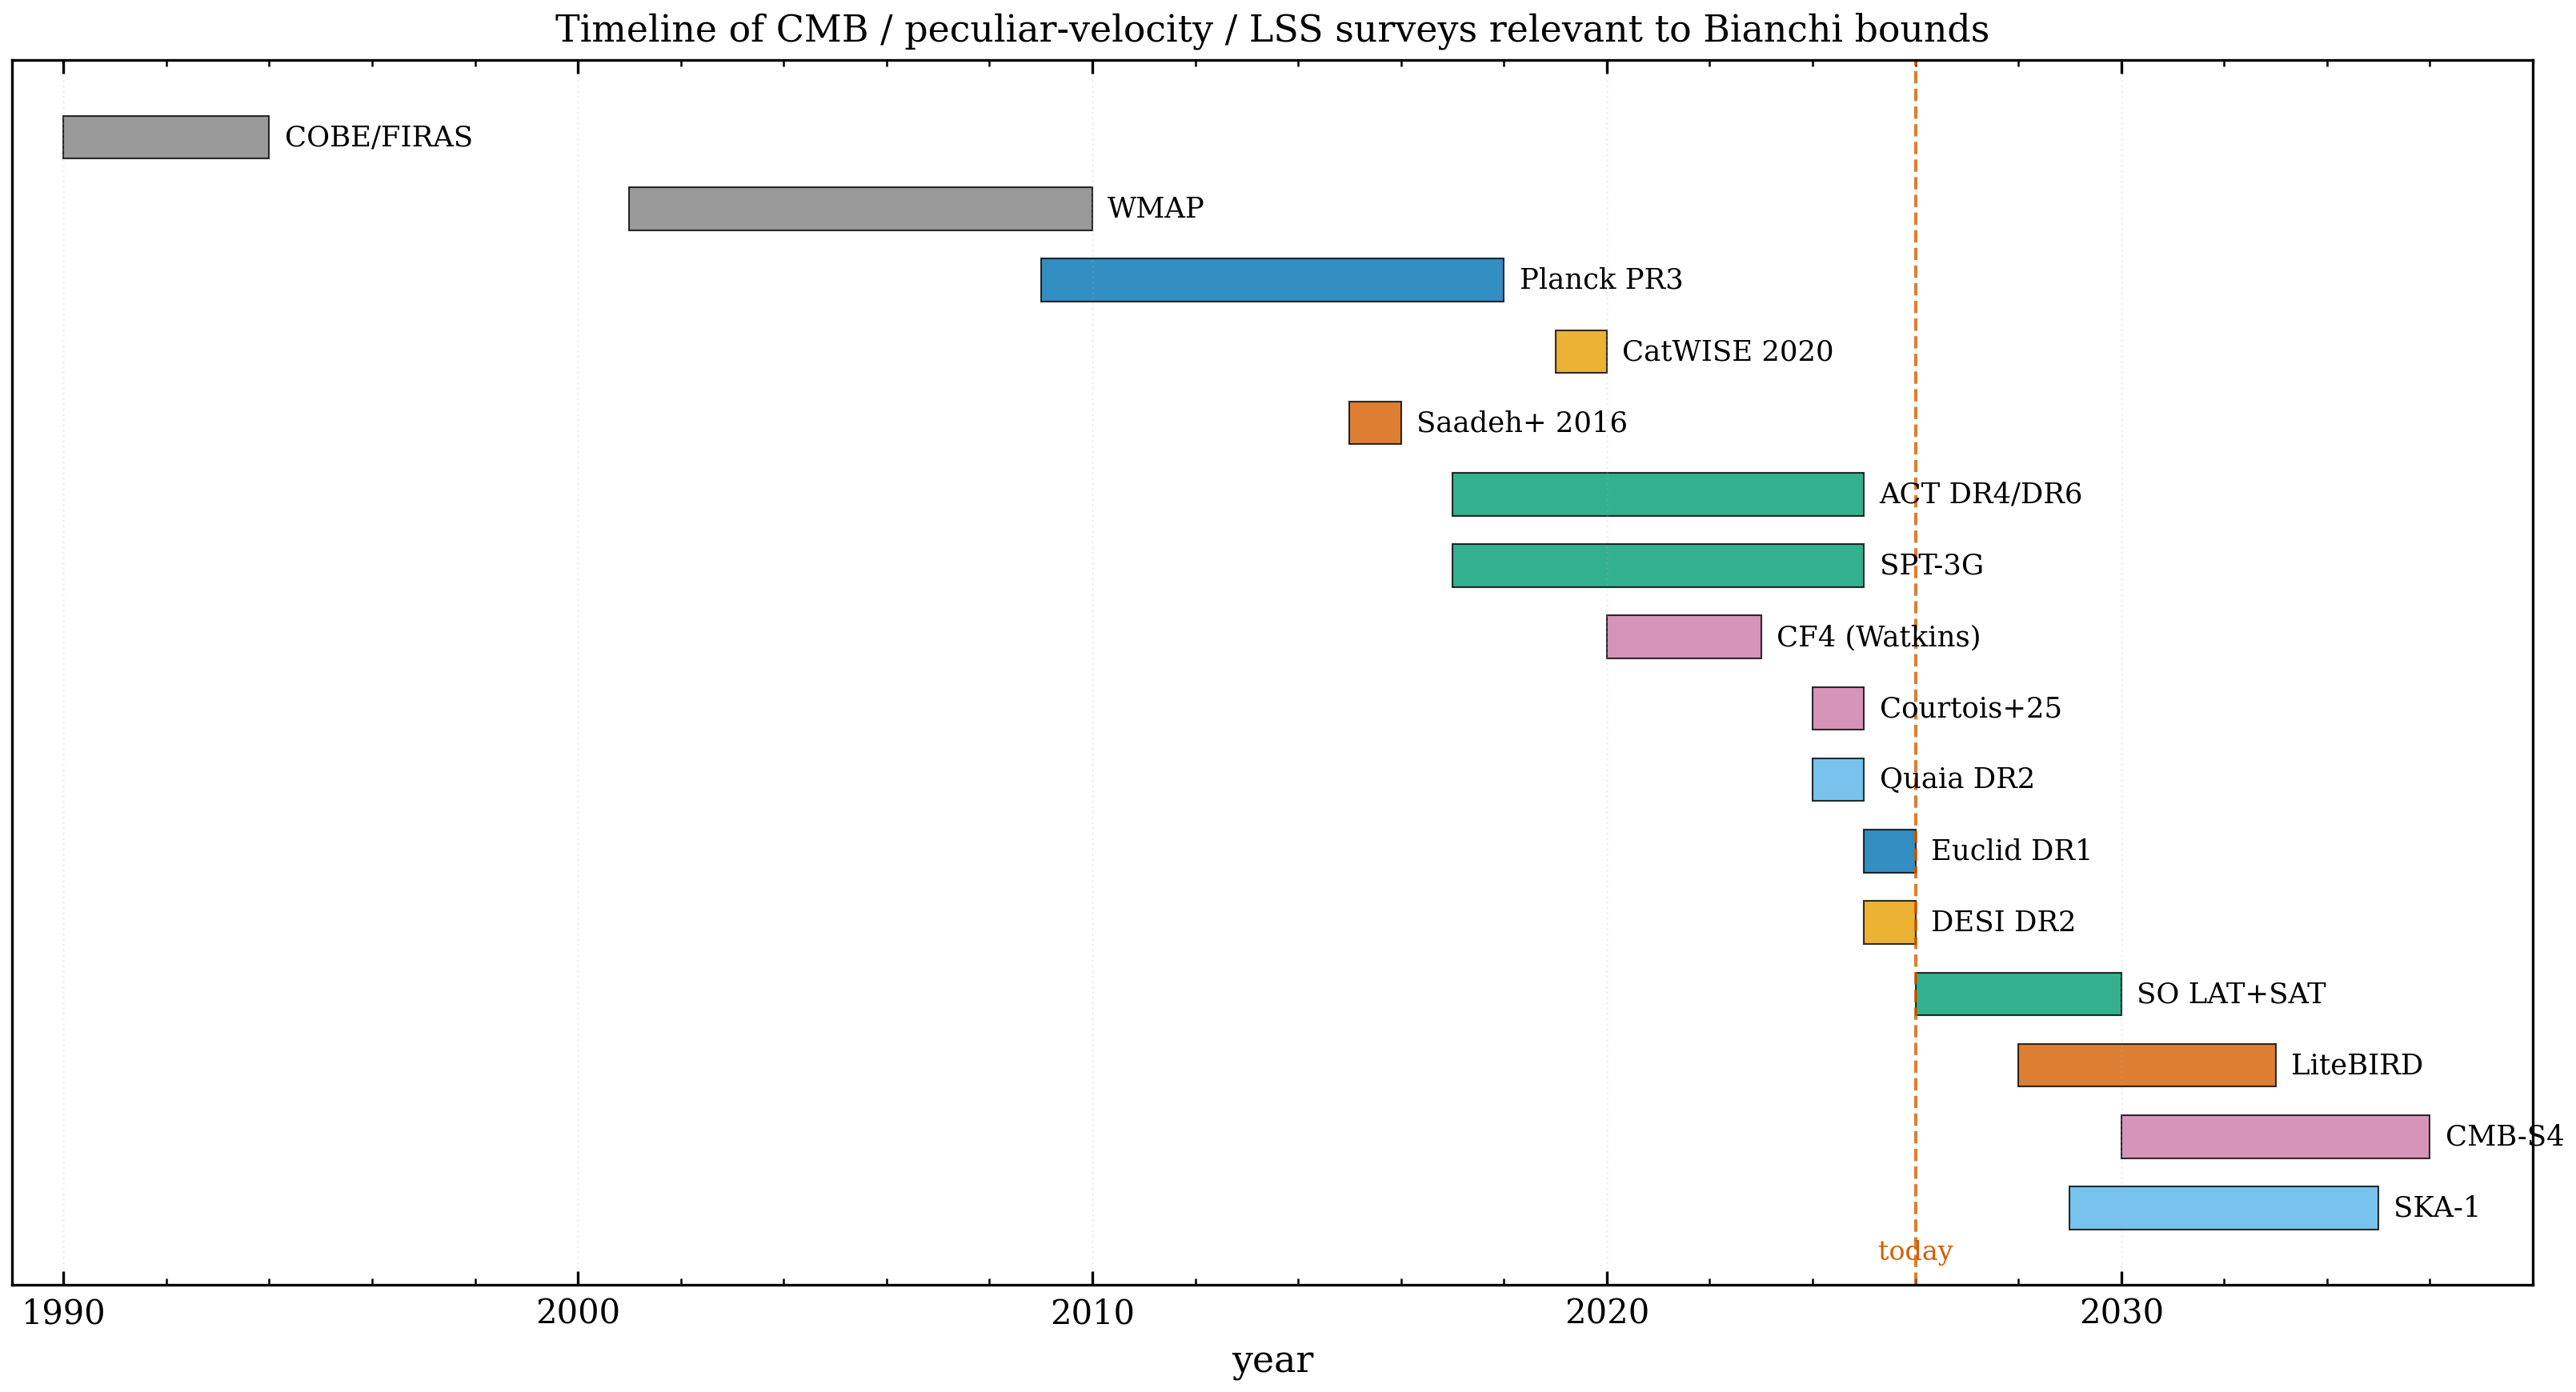
\includegraphics[width=0.82\textwidth,height=0.58\textheight,keepaspectratio]{conditioned_legacy/quarantined-legacy-root-sources__fig_experiment_timeline}
\captionof{figure}{Conditioned legacy diagnostic: experiment timeline. Condition: legacy manuscript-generator assumptions. See sidecar manifest for provenance and caveats; appendix-only, not native-transfer or family-ID evidence.}
\label{fig:conditioned-legacy-quarantined-legacy-root-sources-fig-experiment-timeline}
\end{center}

\clearpage
\begin{center}
\centering
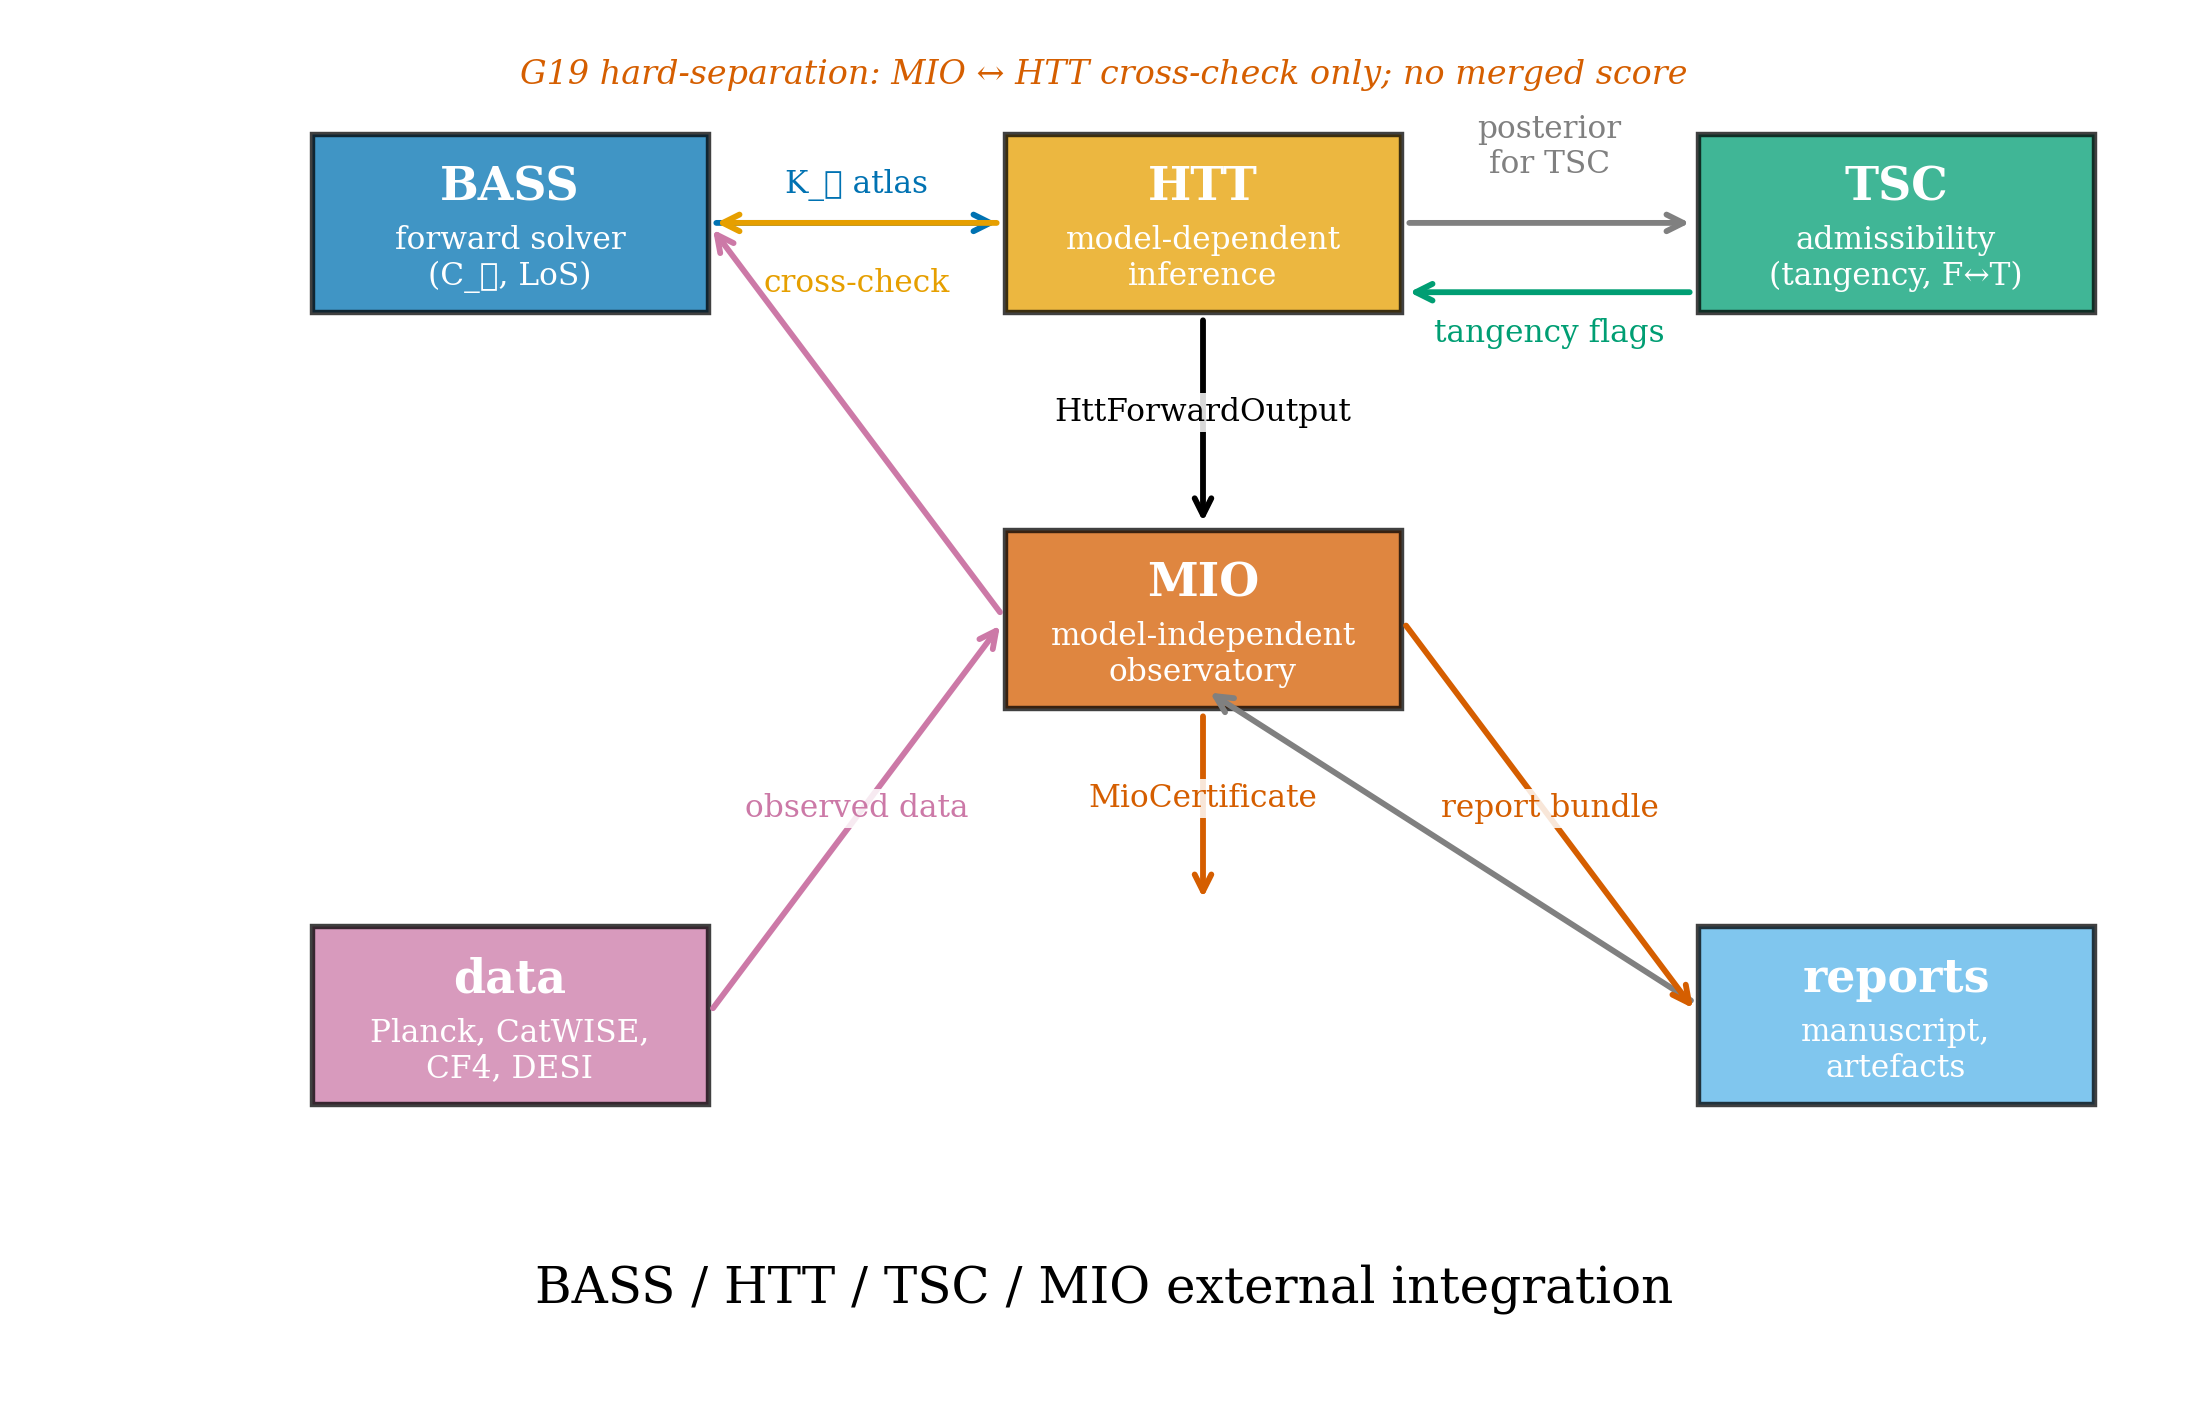
\includegraphics[width=0.82\textwidth,height=0.58\textheight,keepaspectratio]{conditioned_legacy/quarantined-legacy-root-sources__fig_external_integration}
\captionof{figure}{Conditioned legacy diagnostic: external integration. Condition: legacy manuscript-generator assumptions. See sidecar manifest for provenance and caveats; appendix-only, not native-transfer or family-ID evidence.}
\label{fig:conditioned-legacy-quarantined-legacy-root-sources-fig-external-integration}
\end{center}

\clearpage
\begin{center}
\centering
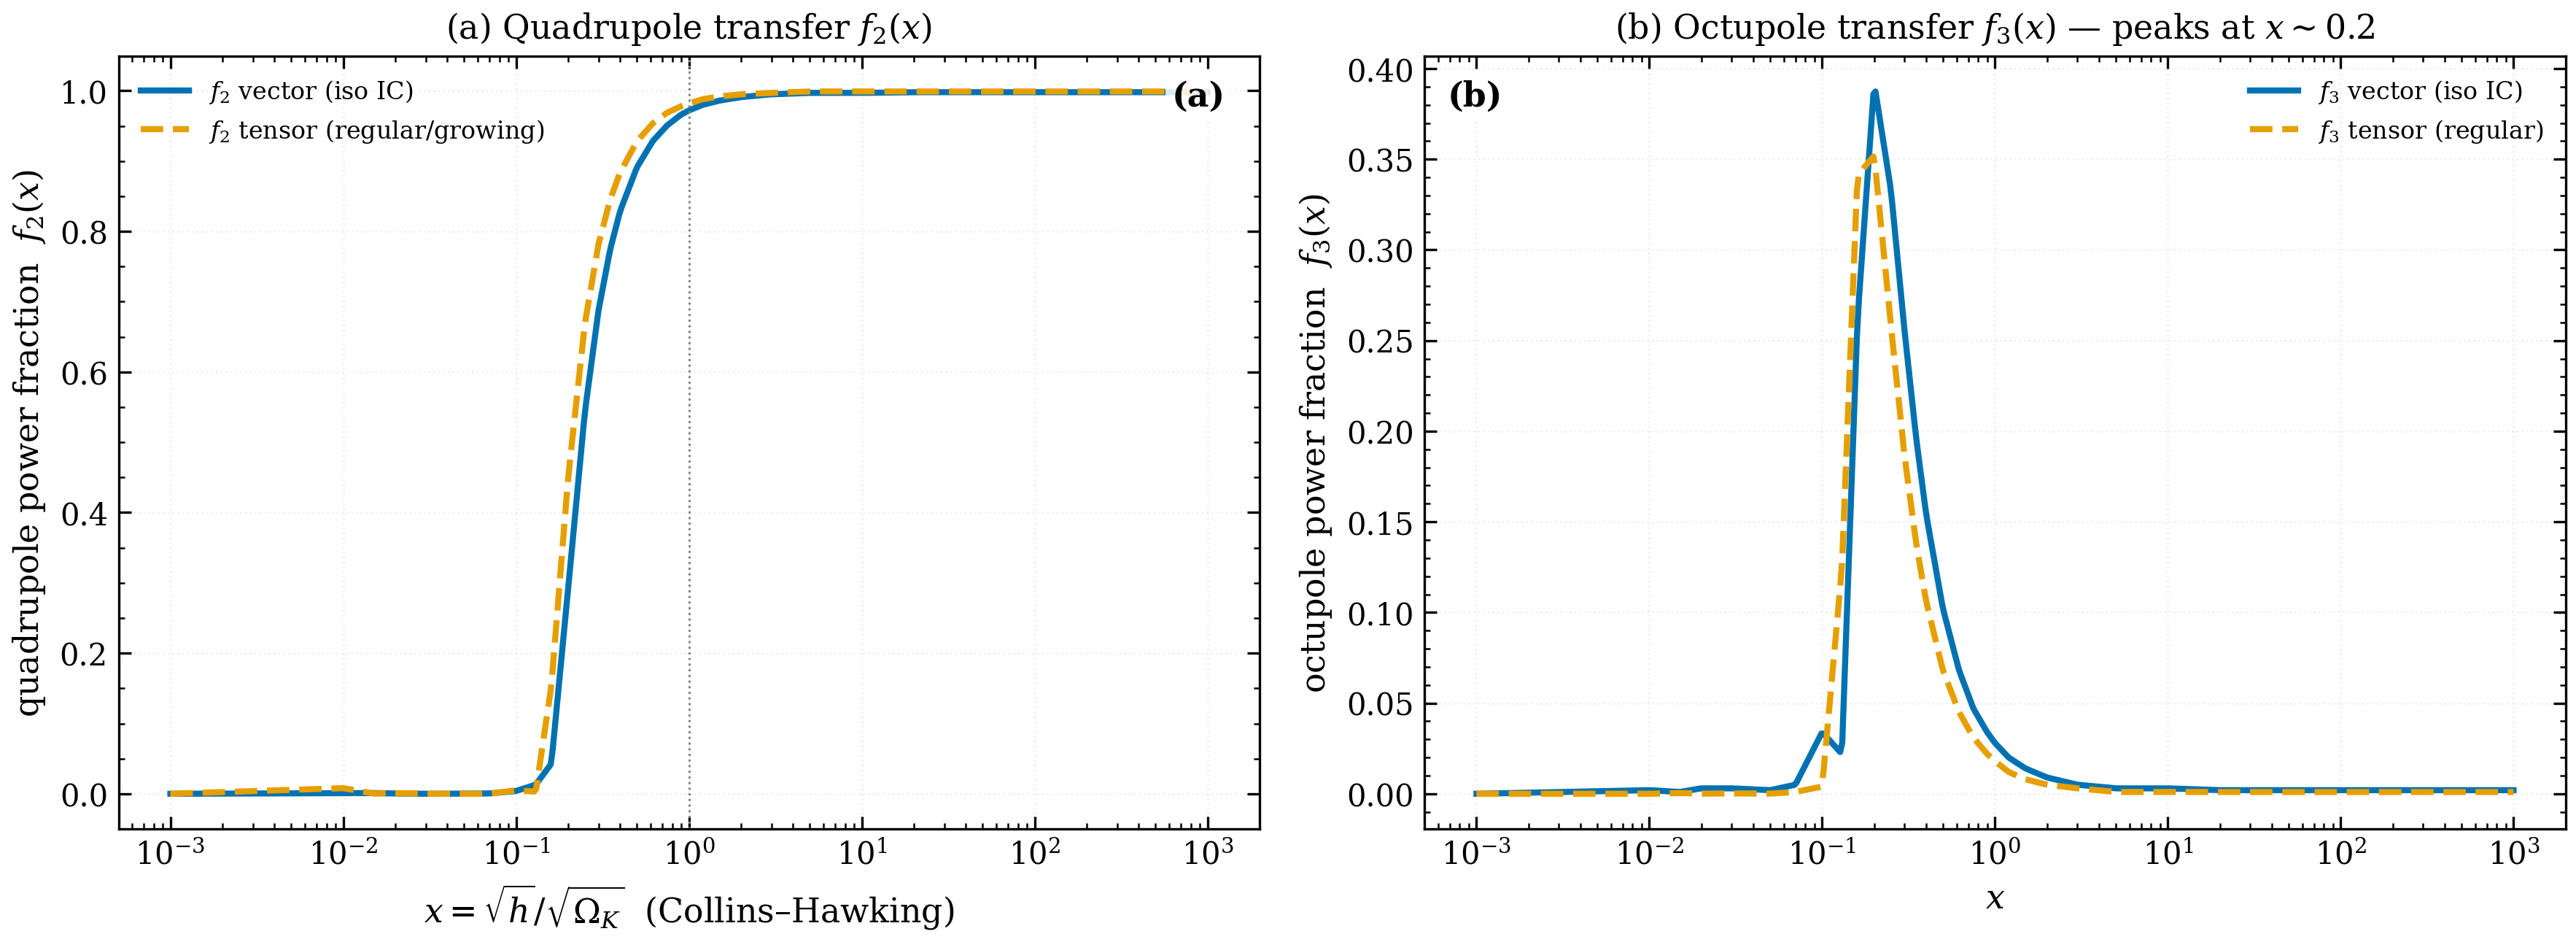
\includegraphics[width=0.82\textwidth,height=0.58\textheight,keepaspectratio]{conditioned_legacy/quarantined-legacy-root-sources__fig_f2_transfer_function}
\captionof{figure}{Conditioned legacy diagnostic: f2 transfer function. Condition: legacy manuscript-generator assumptions. See sidecar manifest for provenance and caveats; appendix-only, not native-transfer or family-ID evidence.}
\label{fig:conditioned-legacy-quarantined-legacy-root-sources-fig-f2-transfer-function}
\end{center}

\clearpage
\begin{center}
\centering
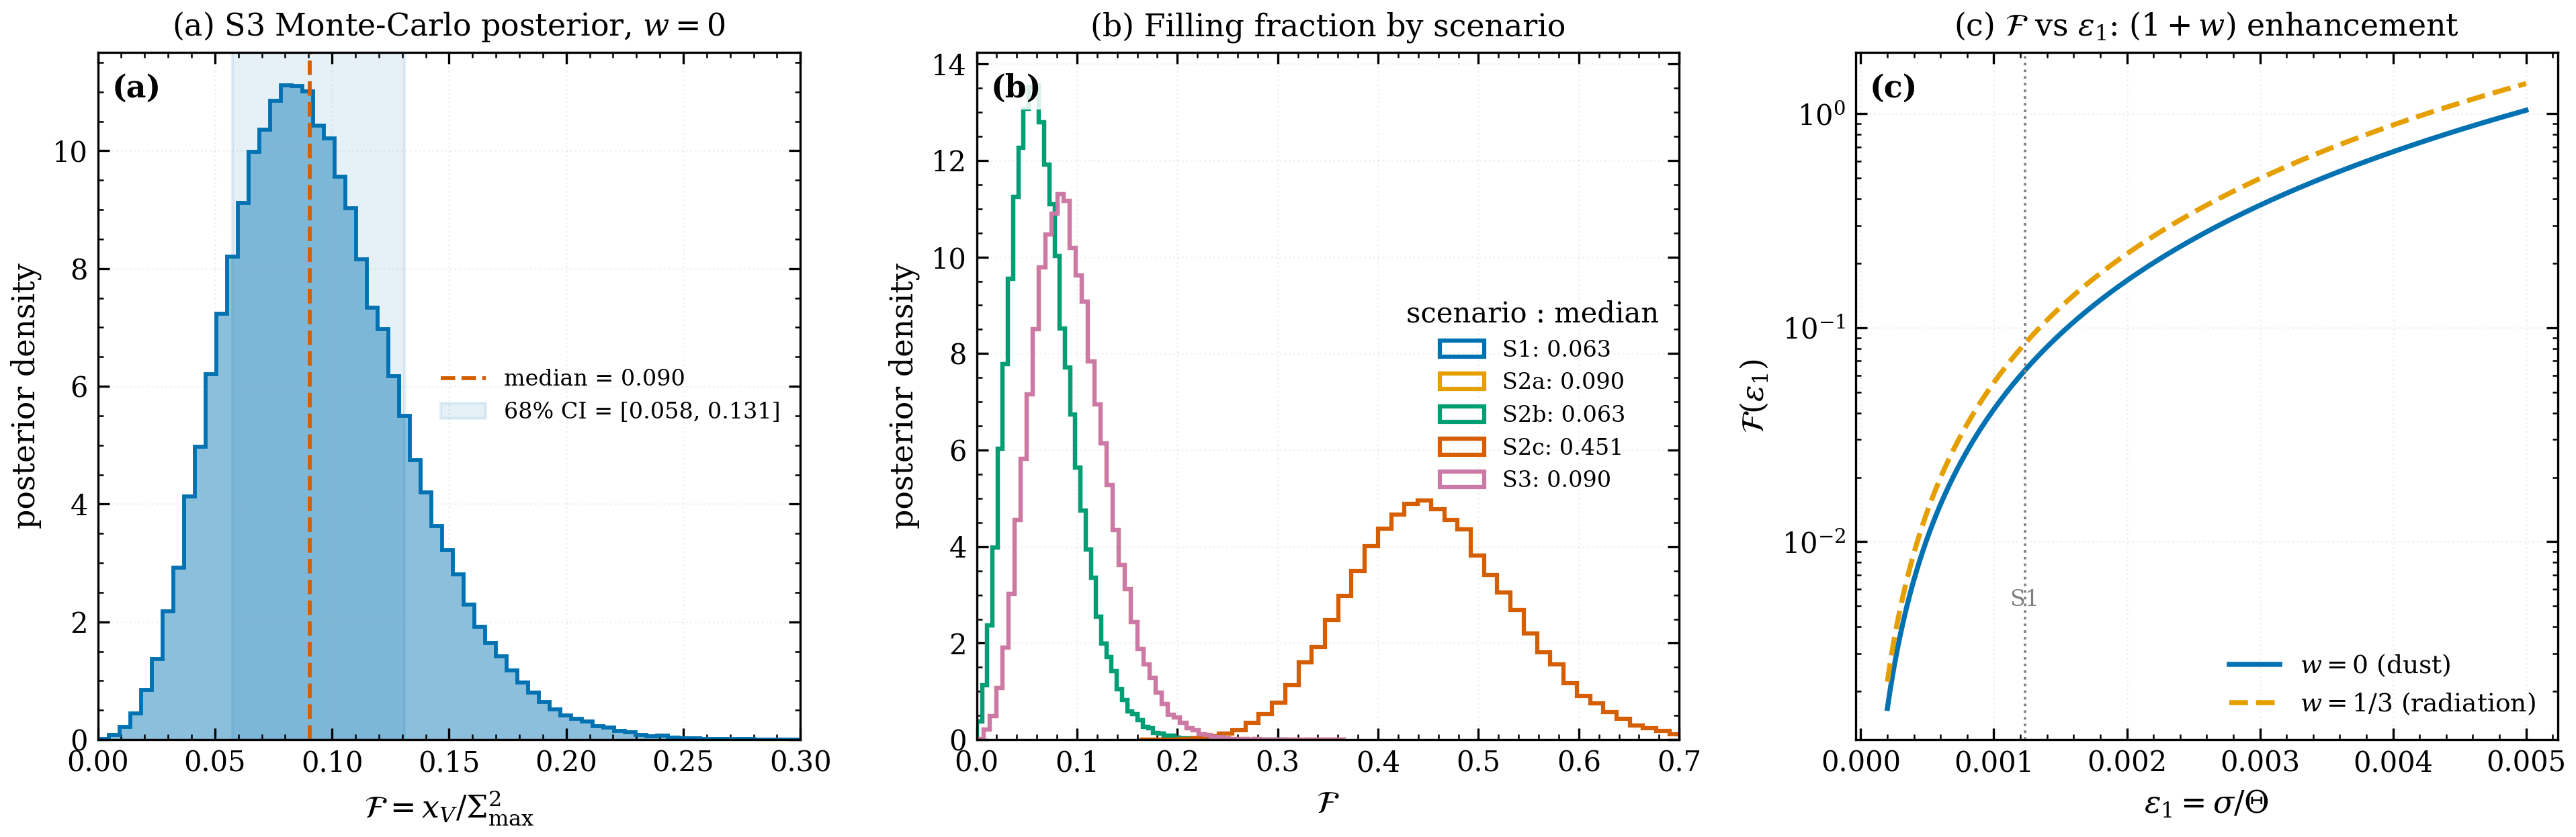
\includegraphics[width=0.82\textwidth,height=0.58\textheight,keepaspectratio]{conditioned_legacy/quarantined-legacy-root-sources__fig_filling_fraction_posterior}
\captionof{figure}{Conditioned legacy diagnostic: filling fraction posterior. Condition: legacy statistical assumptions without current null/PPC/LOOCV refresh. See sidecar manifest for provenance and caveats; appendix-only, not native-transfer or family-ID evidence.}
\label{fig:conditioned-legacy-quarantined-legacy-root-sources-fig-filling-fraction-posterior}
\end{center}

\clearpage
\begin{center}
\centering
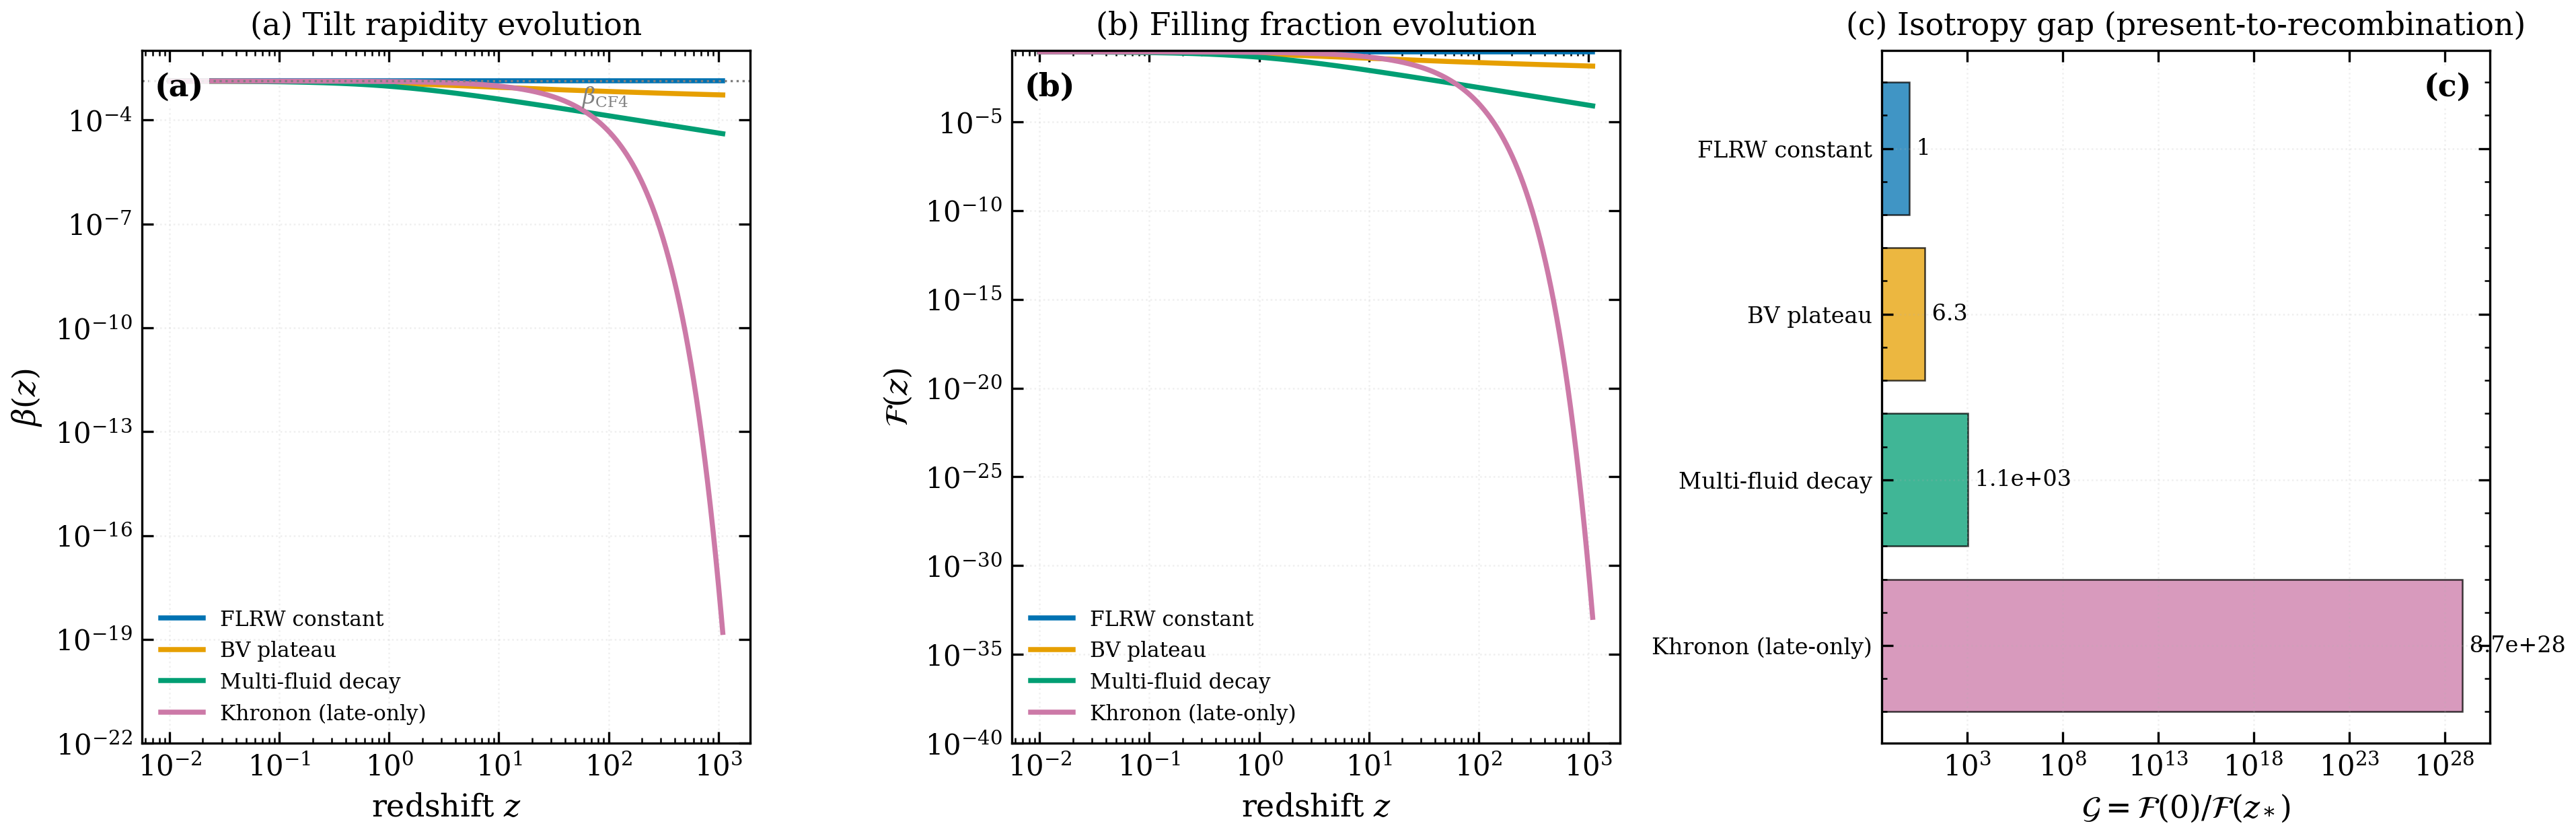
\includegraphics[width=0.82\textwidth,height=0.58\textheight,keepaspectratio]{conditioned_legacy/quarantined-legacy-root-sources__fig_filling_z_evolution}
\captionof{figure}{Conditioned legacy diagnostic: filling z evolution. Condition: legacy manuscript-generator assumptions. See sidecar manifest for provenance and caveats; appendix-only, not native-transfer or family-ID evidence.}
\label{fig:conditioned-legacy-quarantined-legacy-root-sources-fig-filling-z-evolution}
\end{center}

\clearpage
\begin{center}
\centering
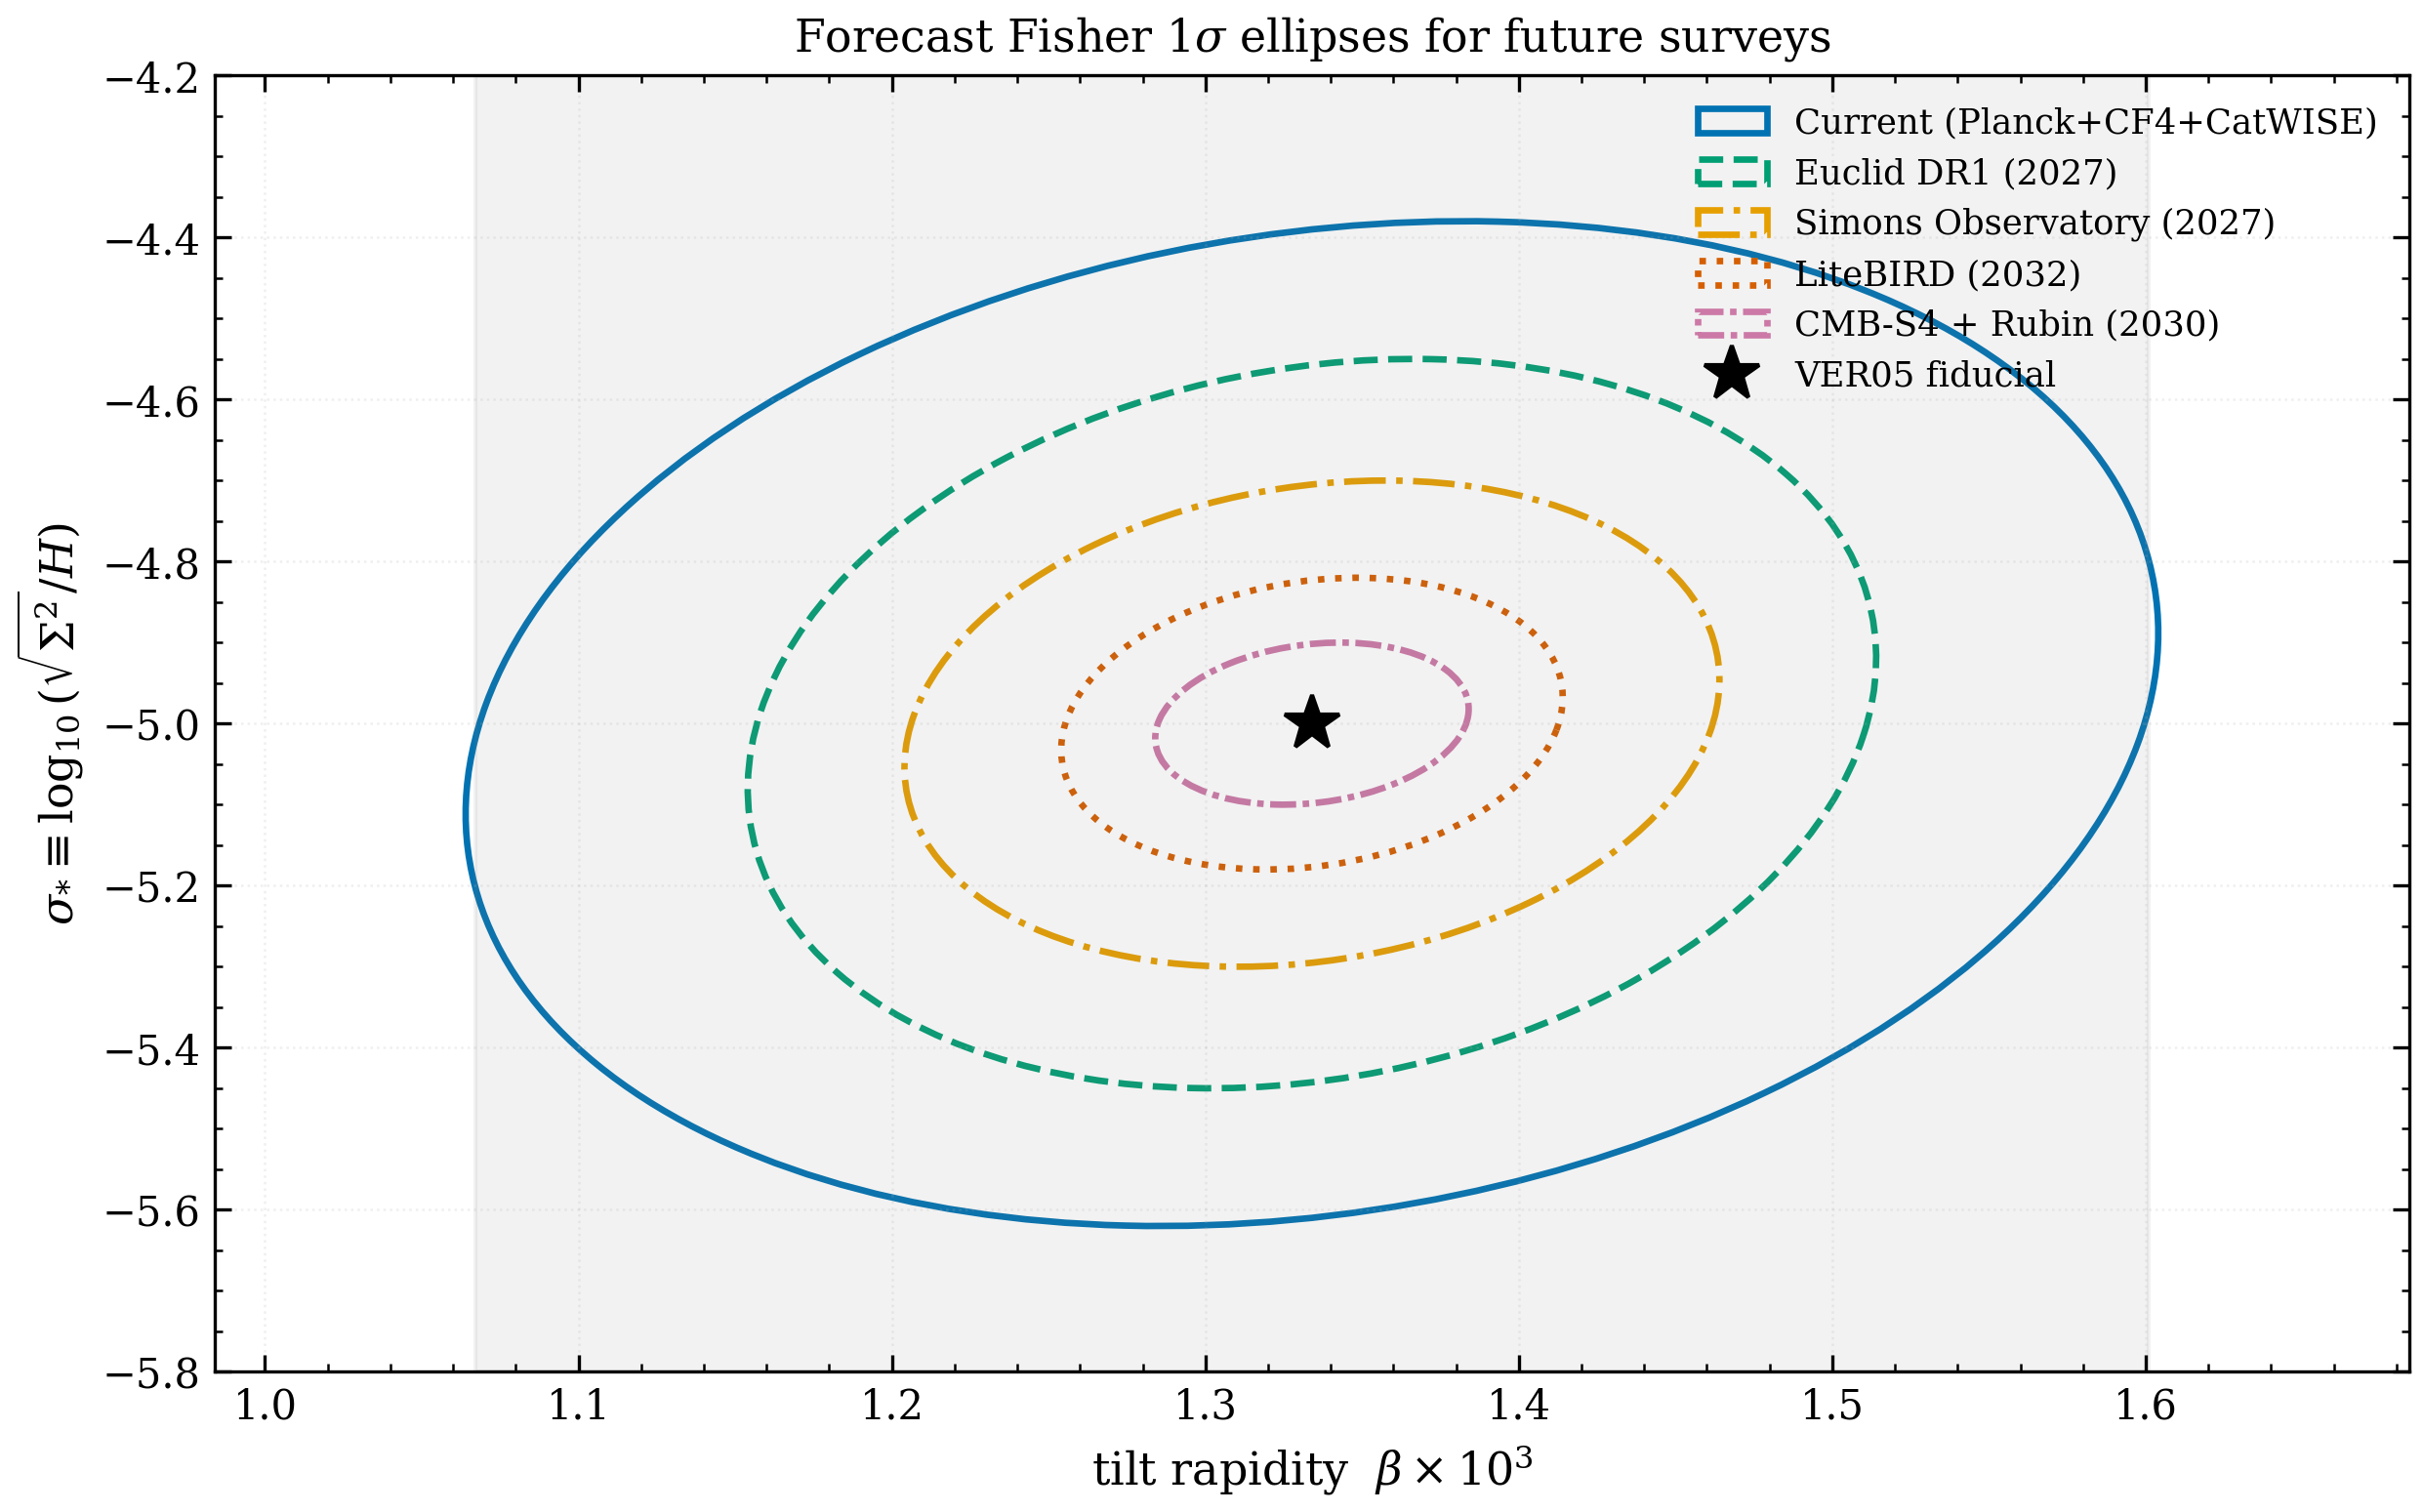
\includegraphics[width=0.82\textwidth,height=0.58\textheight,keepaspectratio]{conditioned_legacy/quarantined-legacy-root-sources__fig_fisher_ellipses_future_surveys}
\captionof{figure}{Conditioned legacy diagnostic: fisher ellipses future surveys. Condition: legacy manuscript-generator assumptions. See sidecar manifest for provenance and caveats; appendix-only, not native-transfer or family-ID evidence.}
\label{fig:conditioned-legacy-quarantined-legacy-root-sources-fig-fisher-ellipses-future-surveys}
\end{center}

\clearpage
\begin{center}
\centering
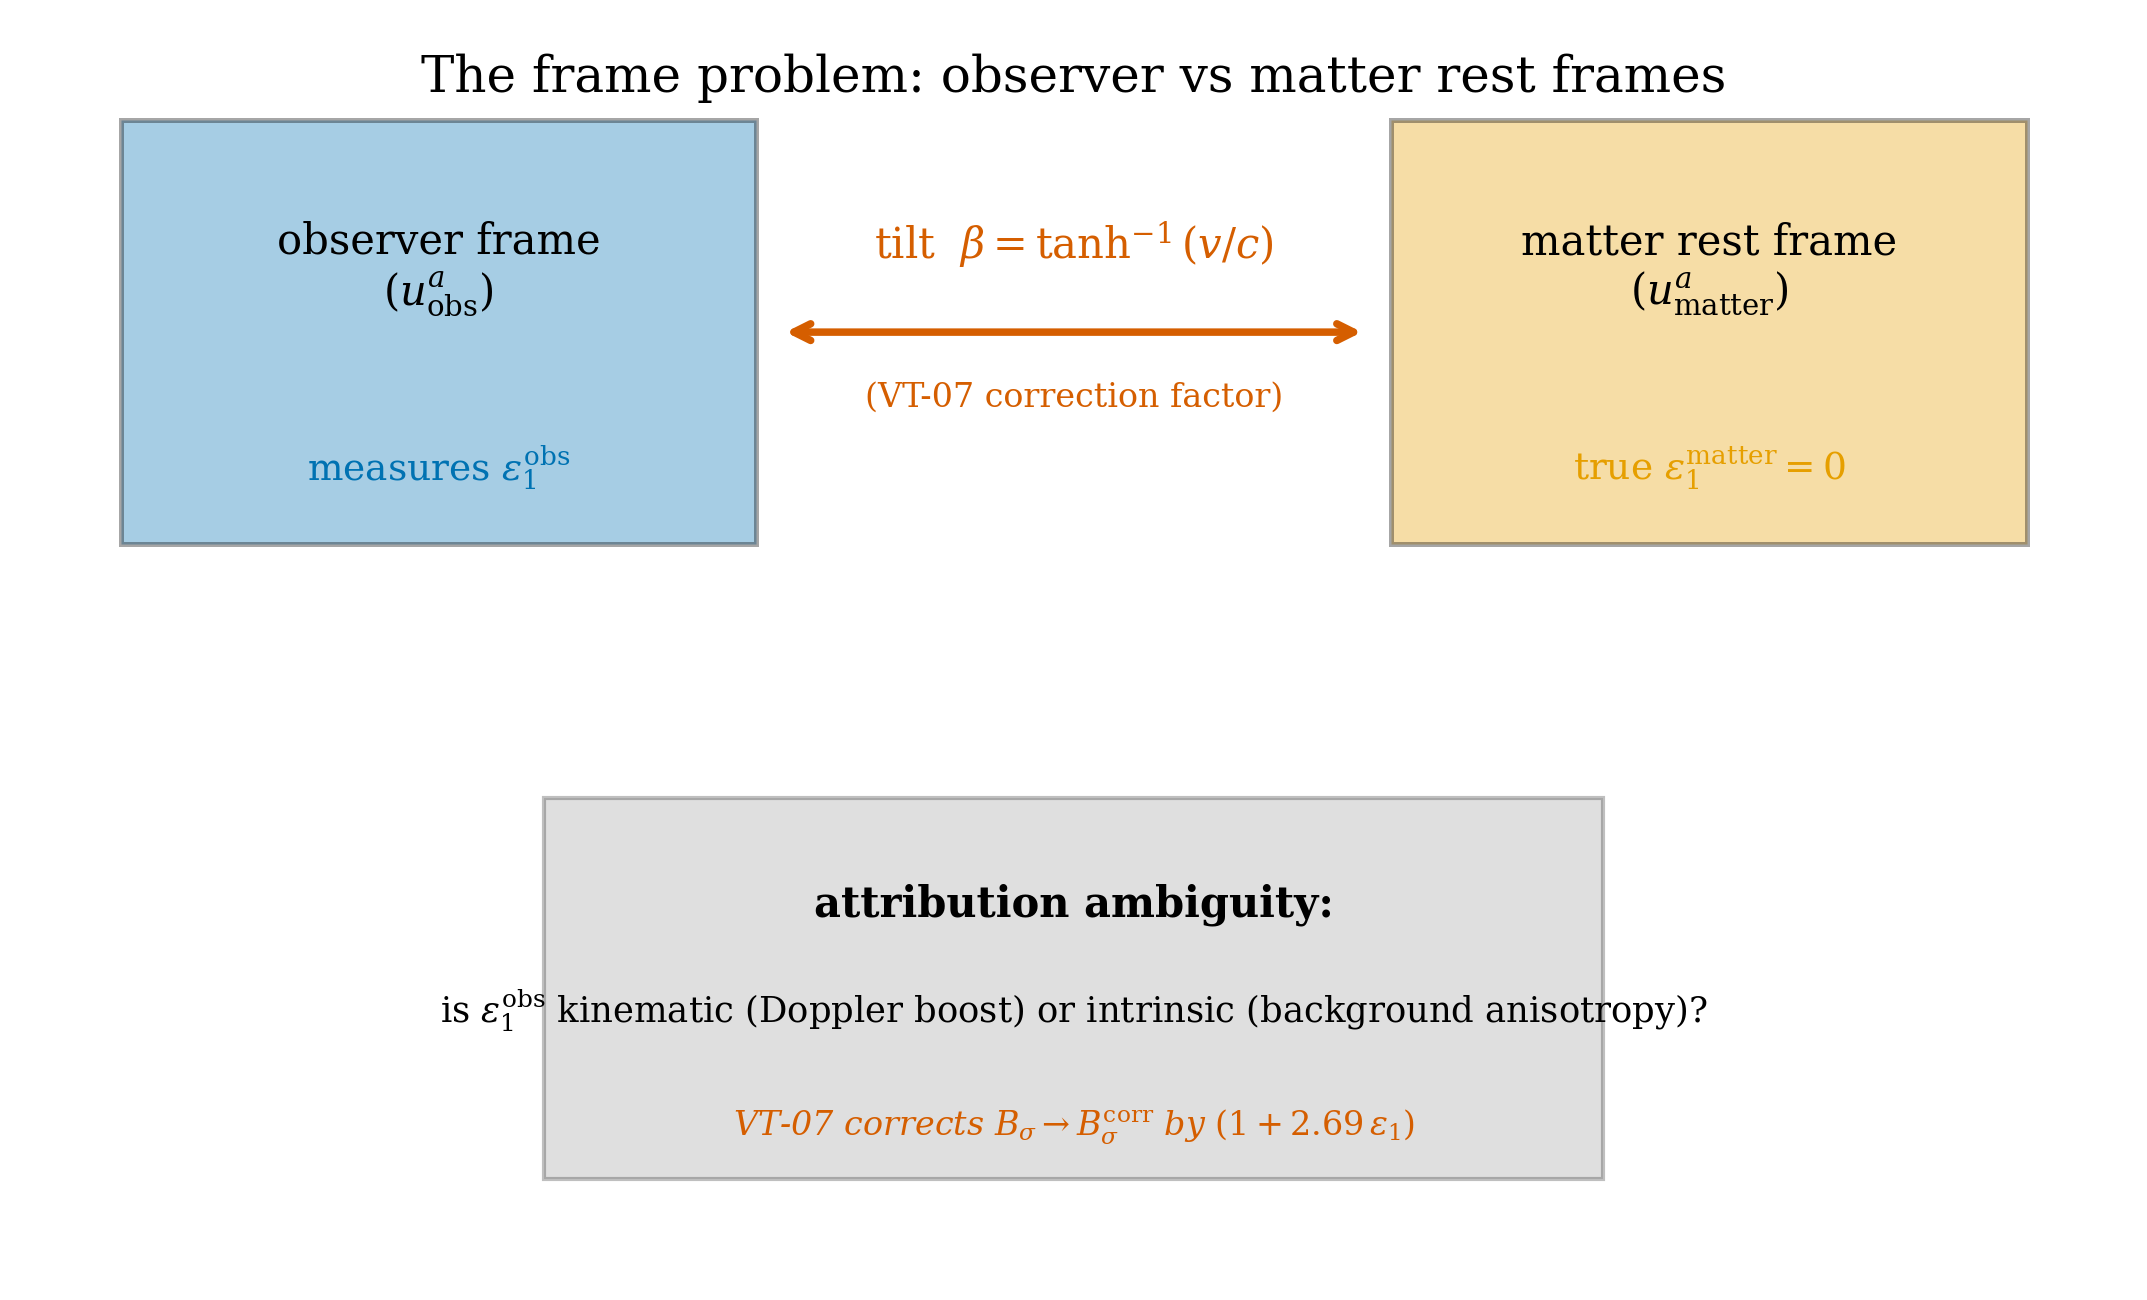
\includegraphics[width=0.82\textwidth,height=0.58\textheight,keepaspectratio]{conditioned_legacy/quarantined-legacy-root-sources__fig_frame_problem}
\captionof{figure}{Conditioned legacy diagnostic: frame problem. Condition: legacy manuscript-generator assumptions. See sidecar manifest for provenance and caveats; appendix-only, not native-transfer or family-ID evidence.}
\label{fig:conditioned-legacy-quarantined-legacy-root-sources-fig-frame-problem}
\end{center}

\clearpage
\begin{center}
\centering
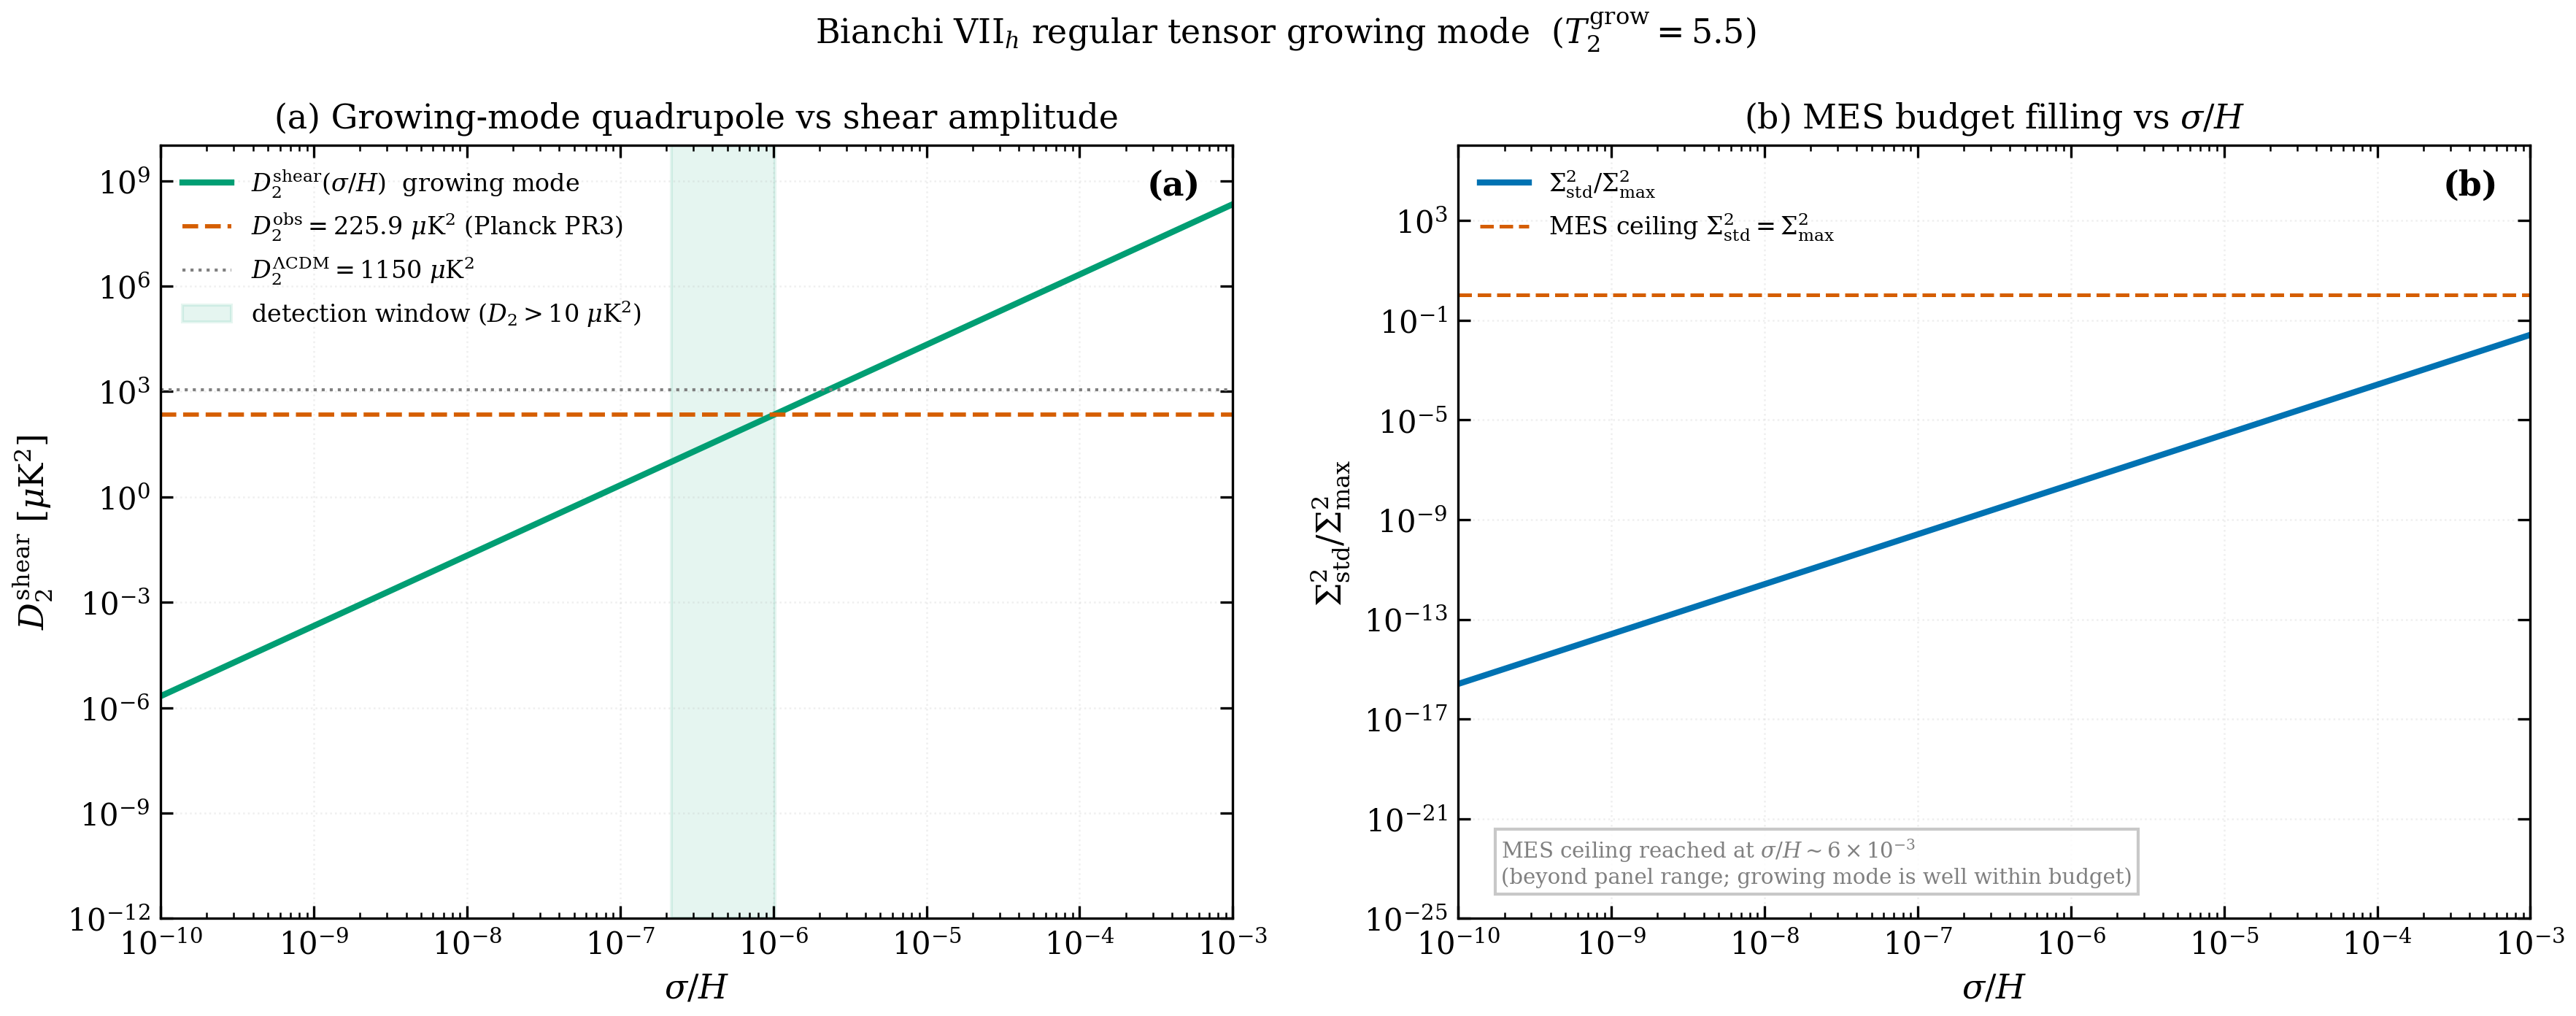
\includegraphics[width=0.82\textwidth,height=0.58\textheight,keepaspectratio]{conditioned_legacy/quarantined-legacy-root-sources__fig_growing_mode}
\captionof{figure}{Conditioned legacy diagnostic: growing mode. Condition: legacy manuscript-generator assumptions. See sidecar manifest for provenance and caveats; appendix-only, not native-transfer or family-ID evidence.}
\label{fig:conditioned-legacy-quarantined-legacy-root-sources-fig-growing-mode}
\end{center}

\clearpage
\begin{center}
\centering
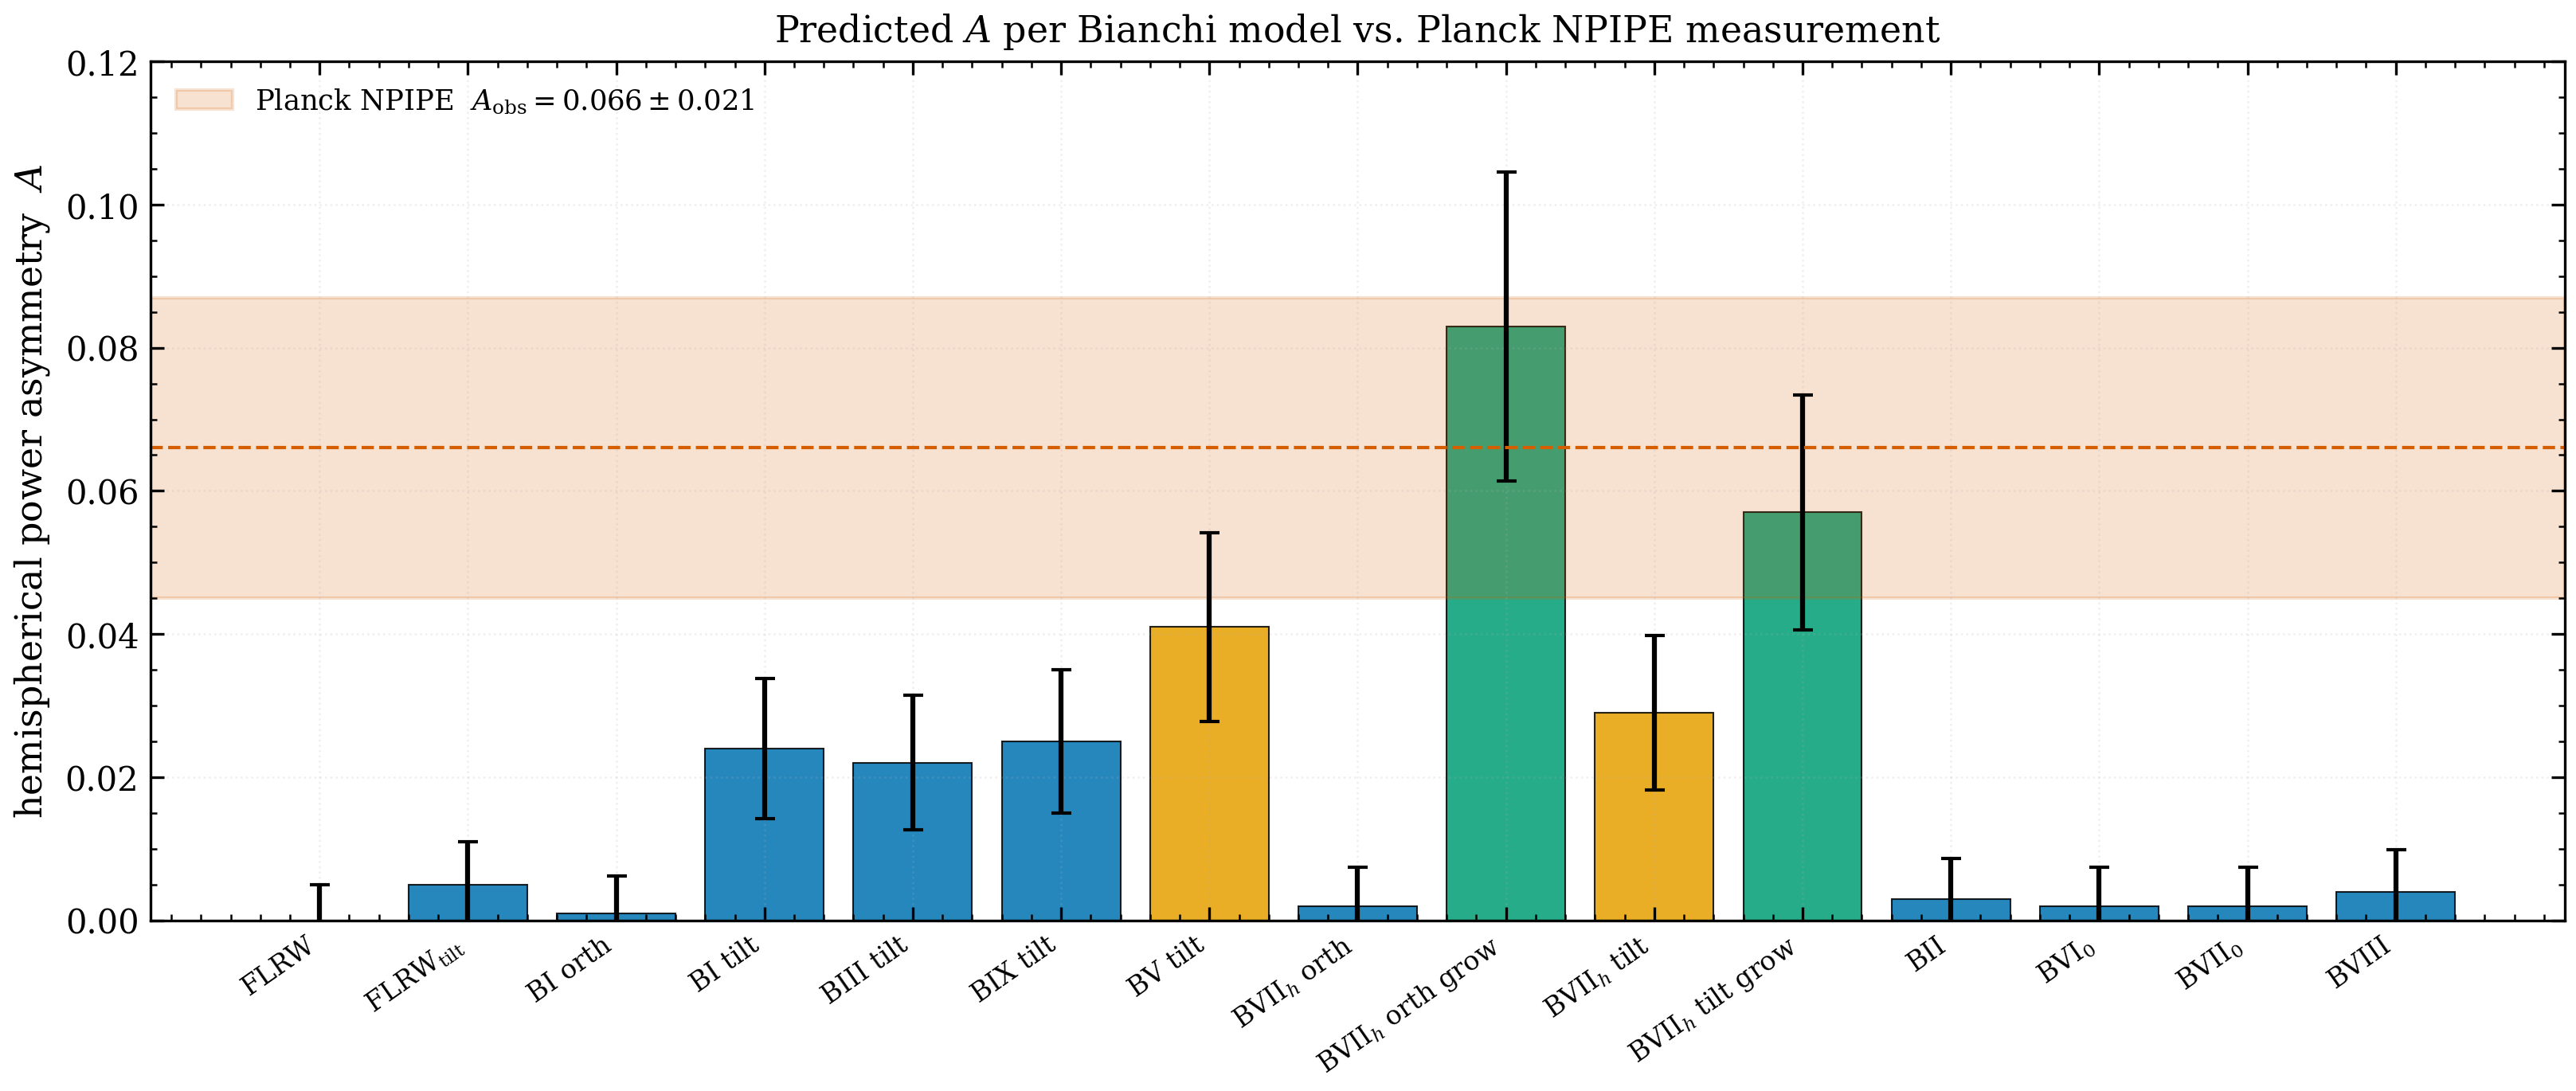
\includegraphics[width=0.82\textwidth,height=0.58\textheight,keepaspectratio]{conditioned_legacy/quarantined-legacy-root-sources__fig_hemispherical_power_asymmetry_bianchi}
\captionof{figure}{Conditioned legacy diagnostic: hemispherical power asymmetry bianchi. Condition: legacy manuscript-generator assumptions. See sidecar manifest for provenance and caveats; appendix-only, not native-transfer or family-ID evidence.}
\label{fig:conditioned-legacy-quarantined-legacy-root-sources-fig-hemispherical-power-asymmetry-bianchi}
\end{center}

\clearpage
\begin{center}
\centering
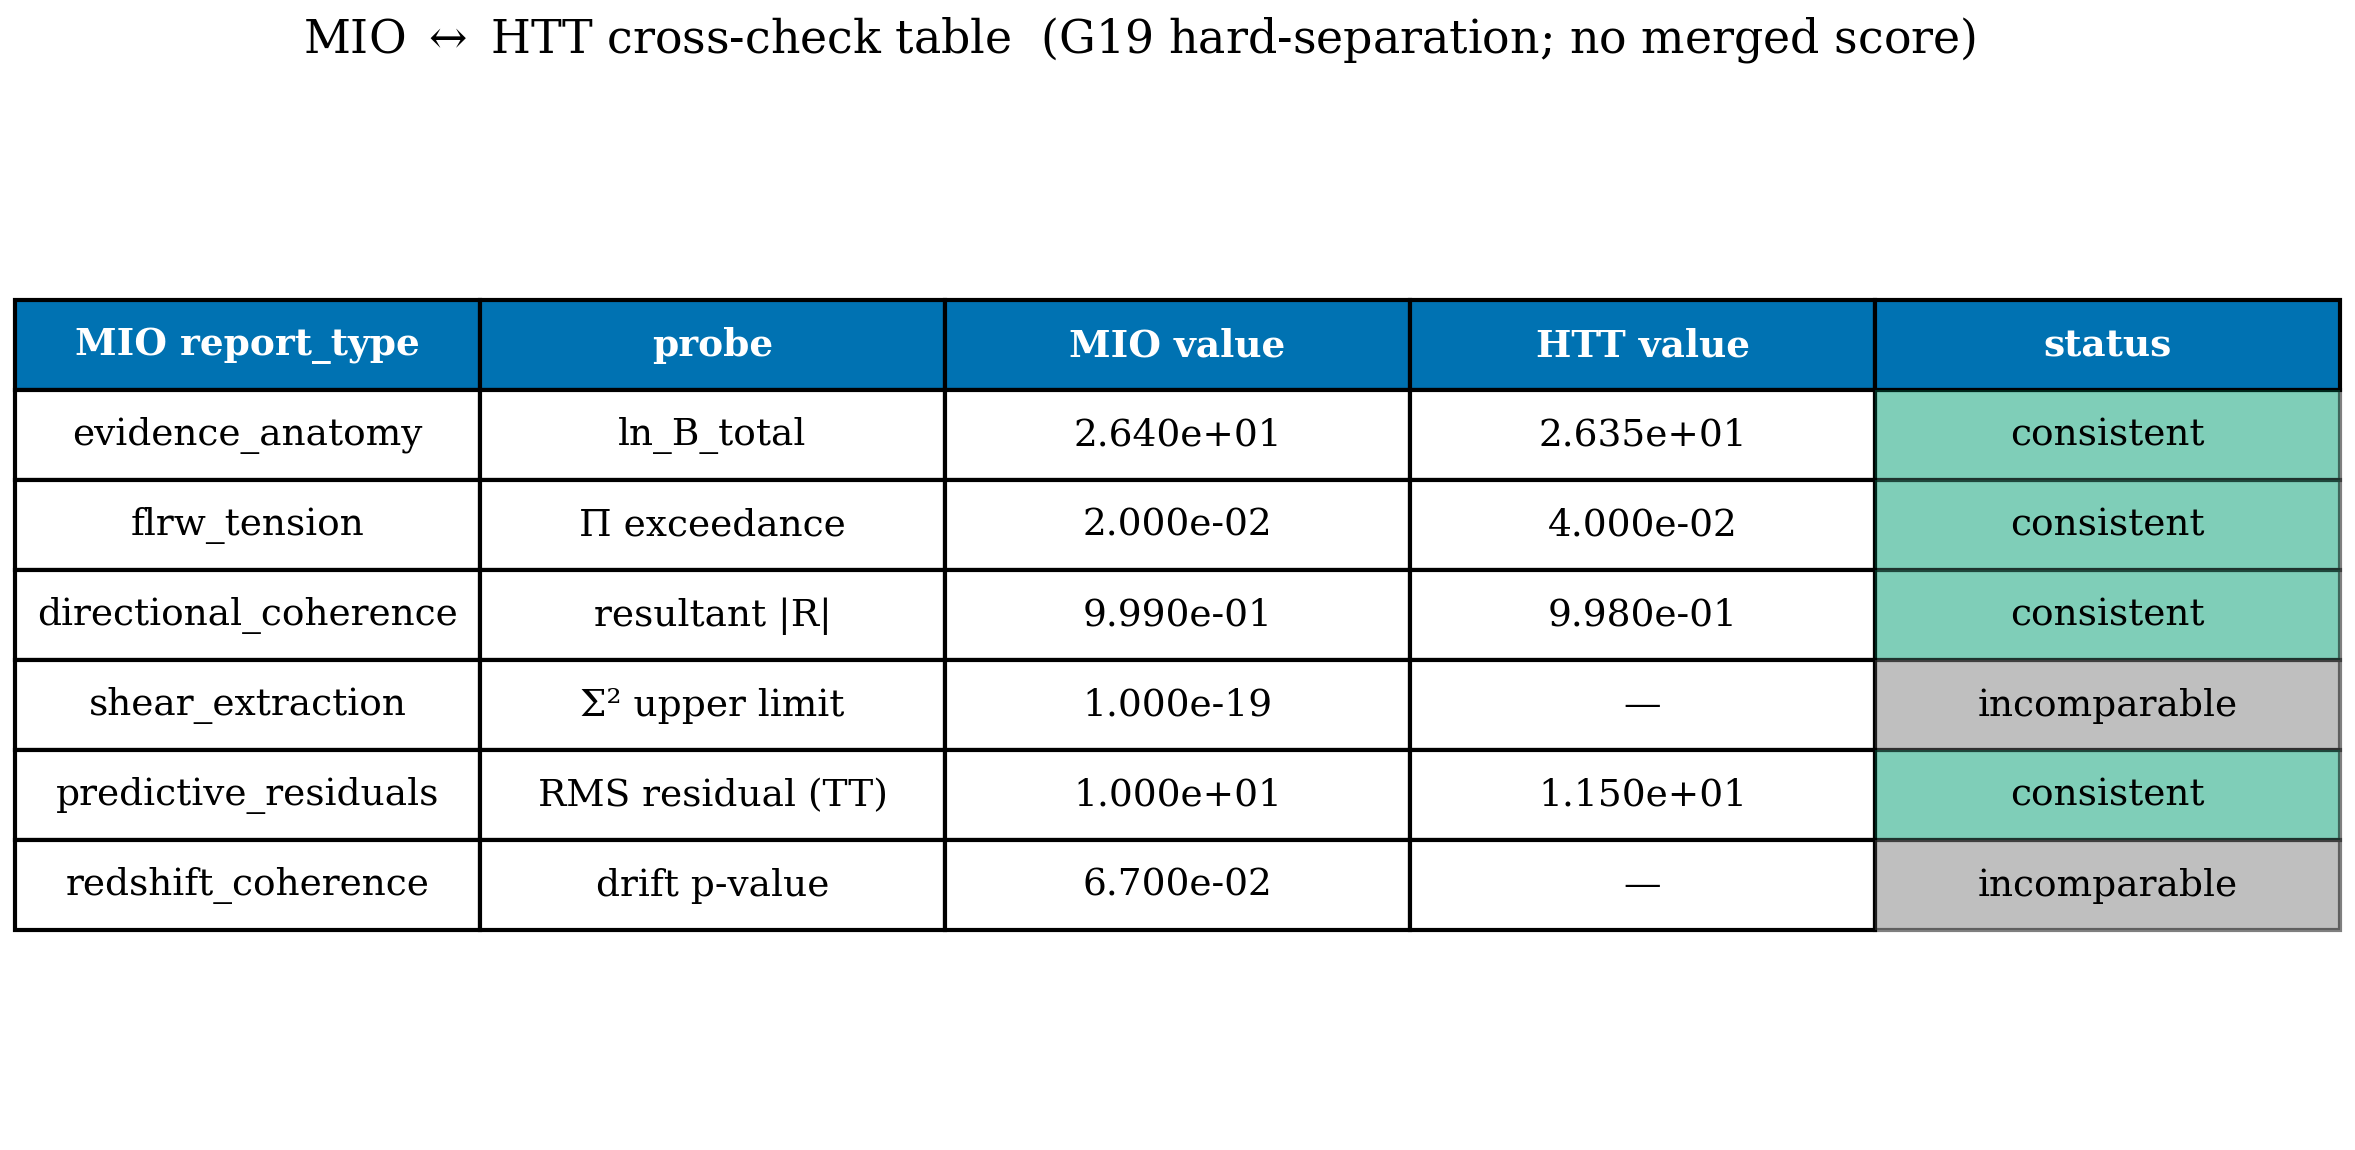
\includegraphics[width=0.82\textwidth,height=0.58\textheight,keepaspectratio]{conditioned_legacy/quarantined-legacy-root-sources__fig_htt_mio_cross_check_table}
\captionof{figure}{Conditioned legacy diagnostic: htt mio cross check table. Condition: legacy manuscript-generator assumptions. See sidecar manifest for provenance and caveats; appendix-only, not native-transfer or family-ID evidence.}
\label{fig:conditioned-legacy-quarantined-legacy-root-sources-fig-htt-mio-cross-check-table}
\end{center}

\clearpage
\begin{center}
\centering
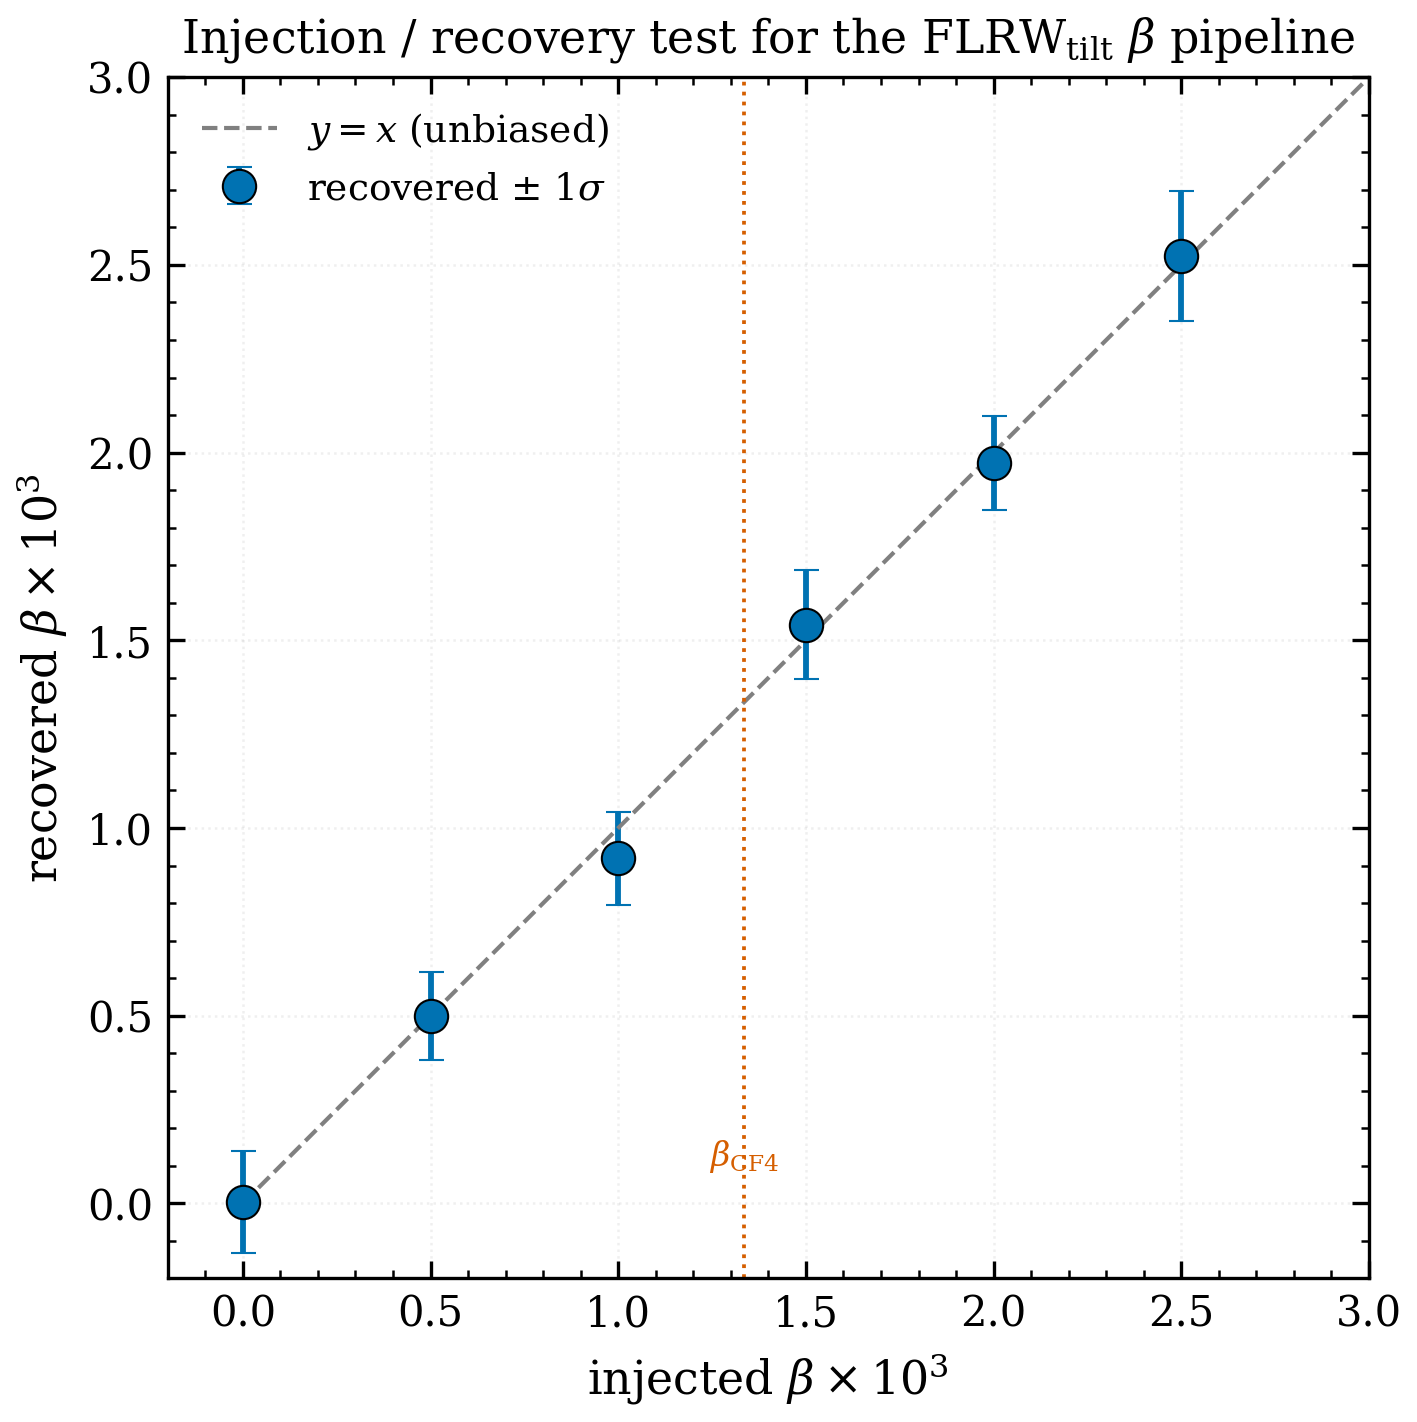
\includegraphics[width=0.82\textwidth,height=0.58\textheight,keepaspectratio]{conditioned_legacy/quarantined-legacy-root-sources__fig_injection_recovery}
\captionof{figure}{Conditioned legacy diagnostic: injection recovery. Condition: legacy manuscript-generator assumptions. See sidecar manifest for provenance and caveats; appendix-only, not native-transfer or family-ID evidence.}
\label{fig:conditioned-legacy-quarantined-legacy-root-sources-fig-injection-recovery}
\end{center}

\clearpage
\begin{center}
\centering
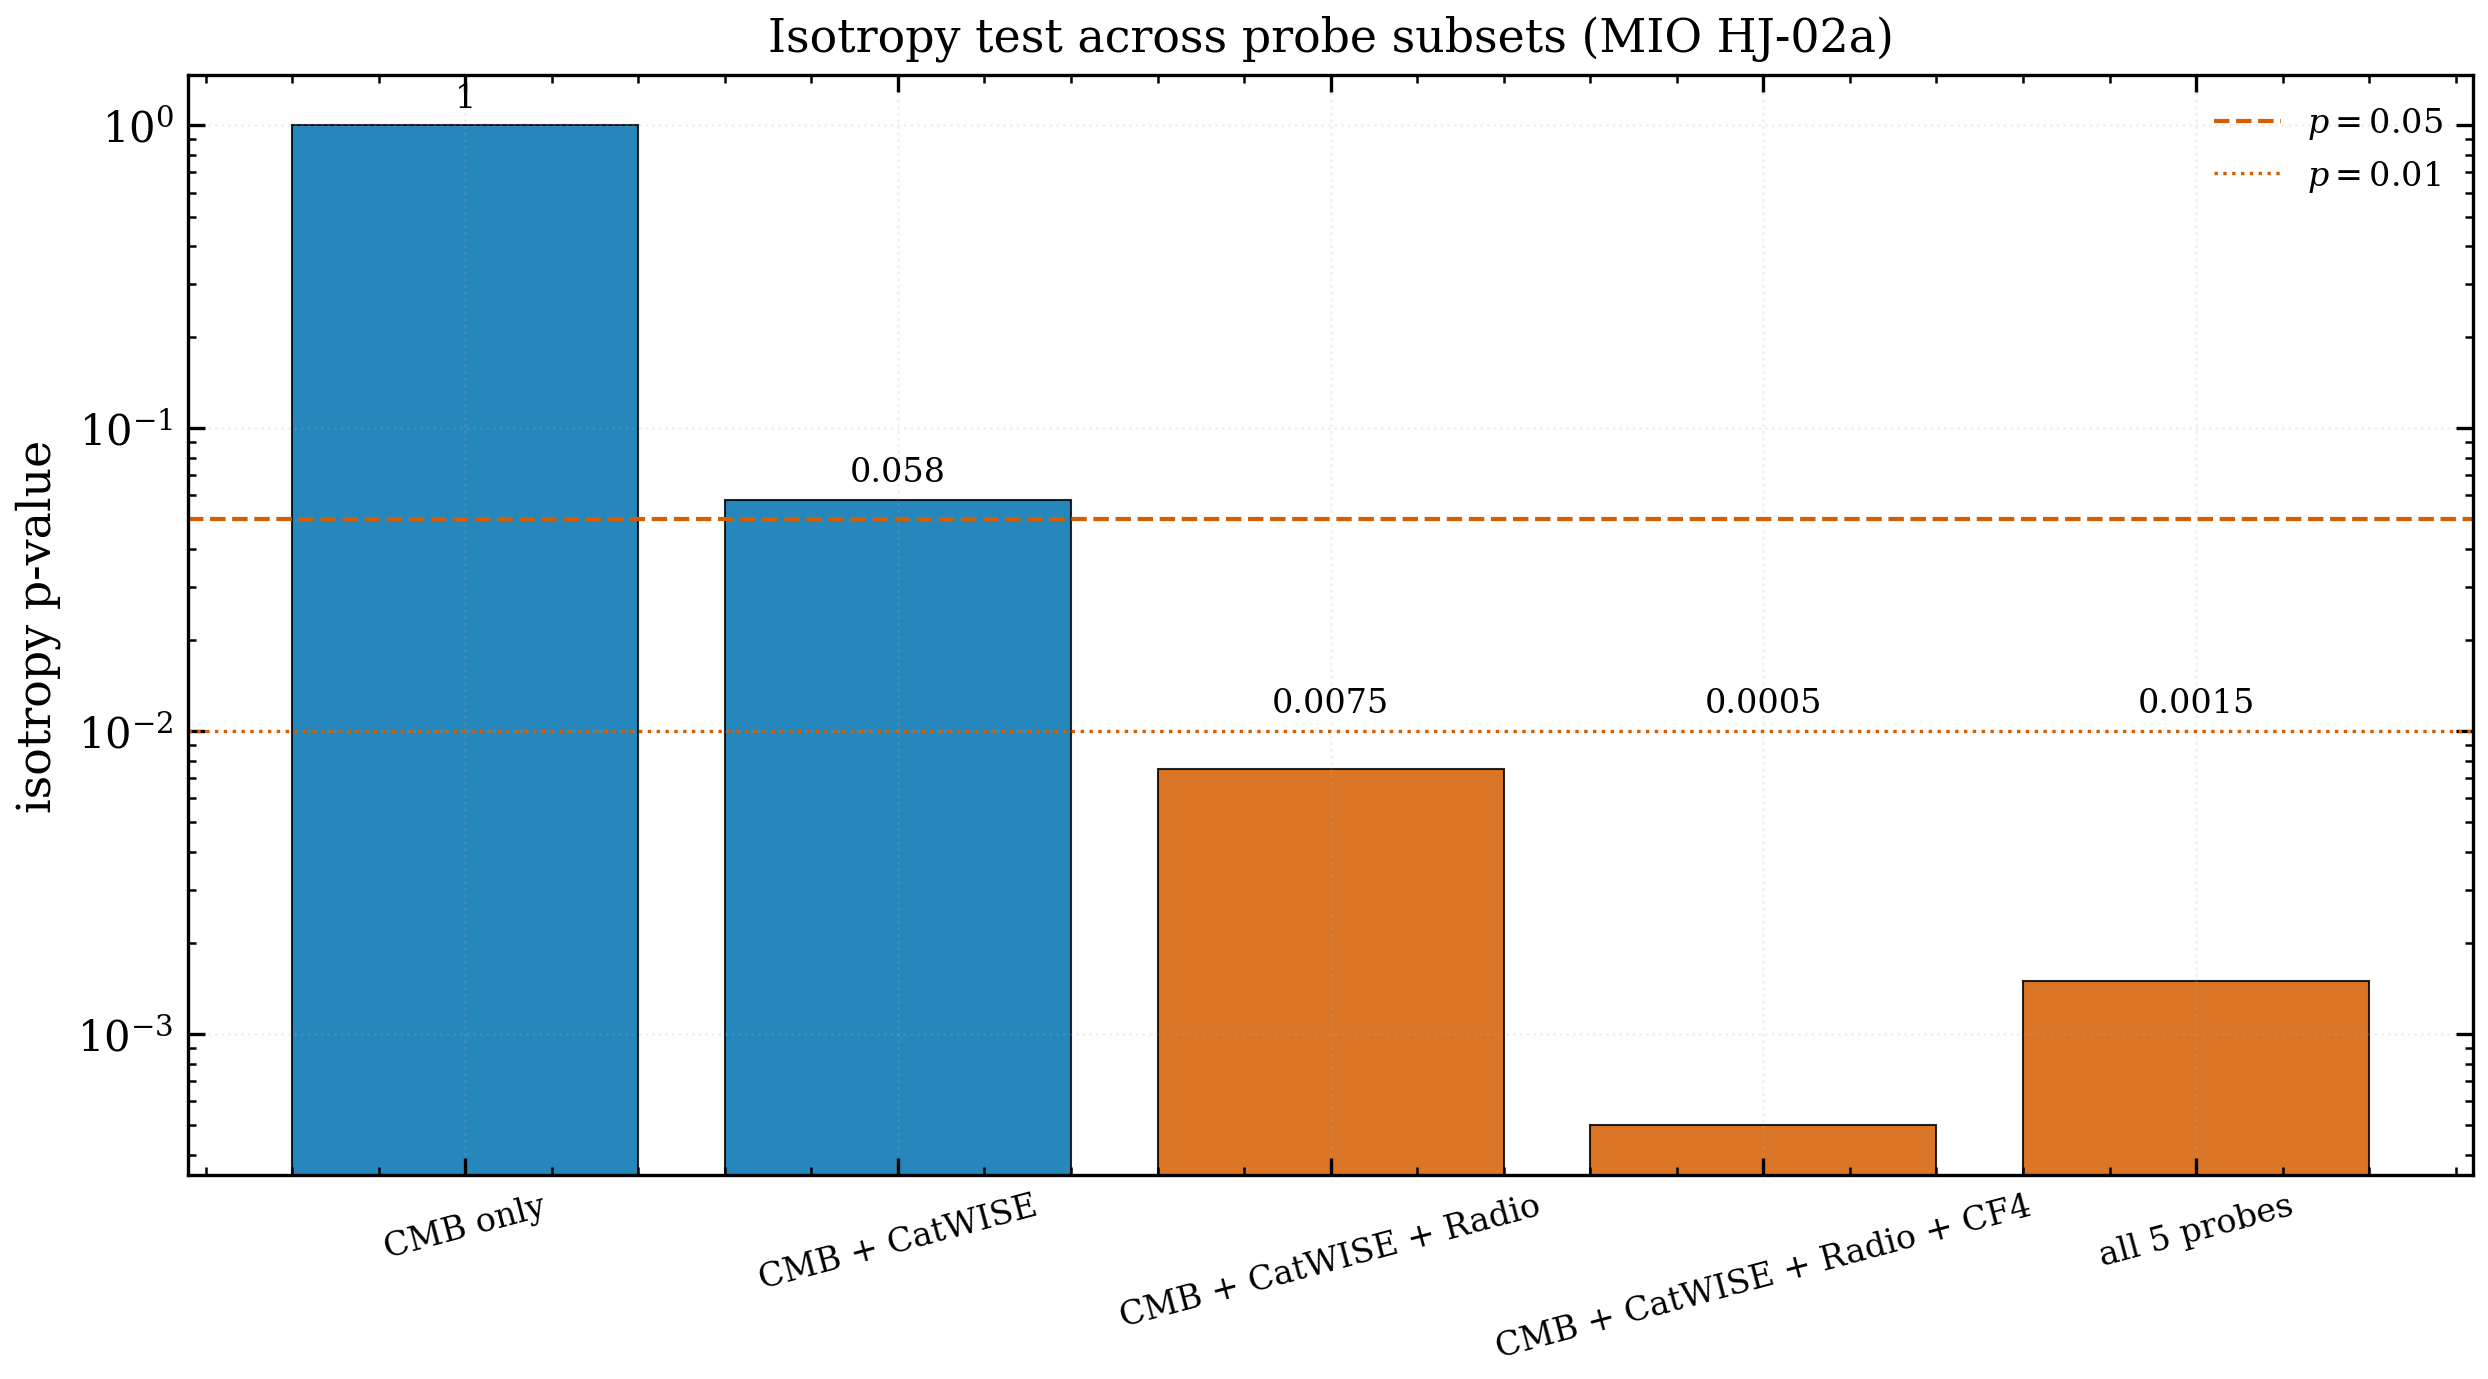
\includegraphics[width=0.82\textwidth,height=0.58\textheight,keepaspectratio]{conditioned_legacy/quarantined-legacy-root-sources__fig_isotropy_pvalue_per_combination}
\captionof{figure}{Conditioned legacy diagnostic: isotropy pvalue per combination. Condition: legacy manuscript-generator assumptions. See sidecar manifest for provenance and caveats; appendix-only, not native-transfer or family-ID evidence.}
\label{fig:conditioned-legacy-quarantined-legacy-root-sources-fig-isotropy-pvalue-per-combination}
\end{center}

\clearpage
\begin{center}
\centering
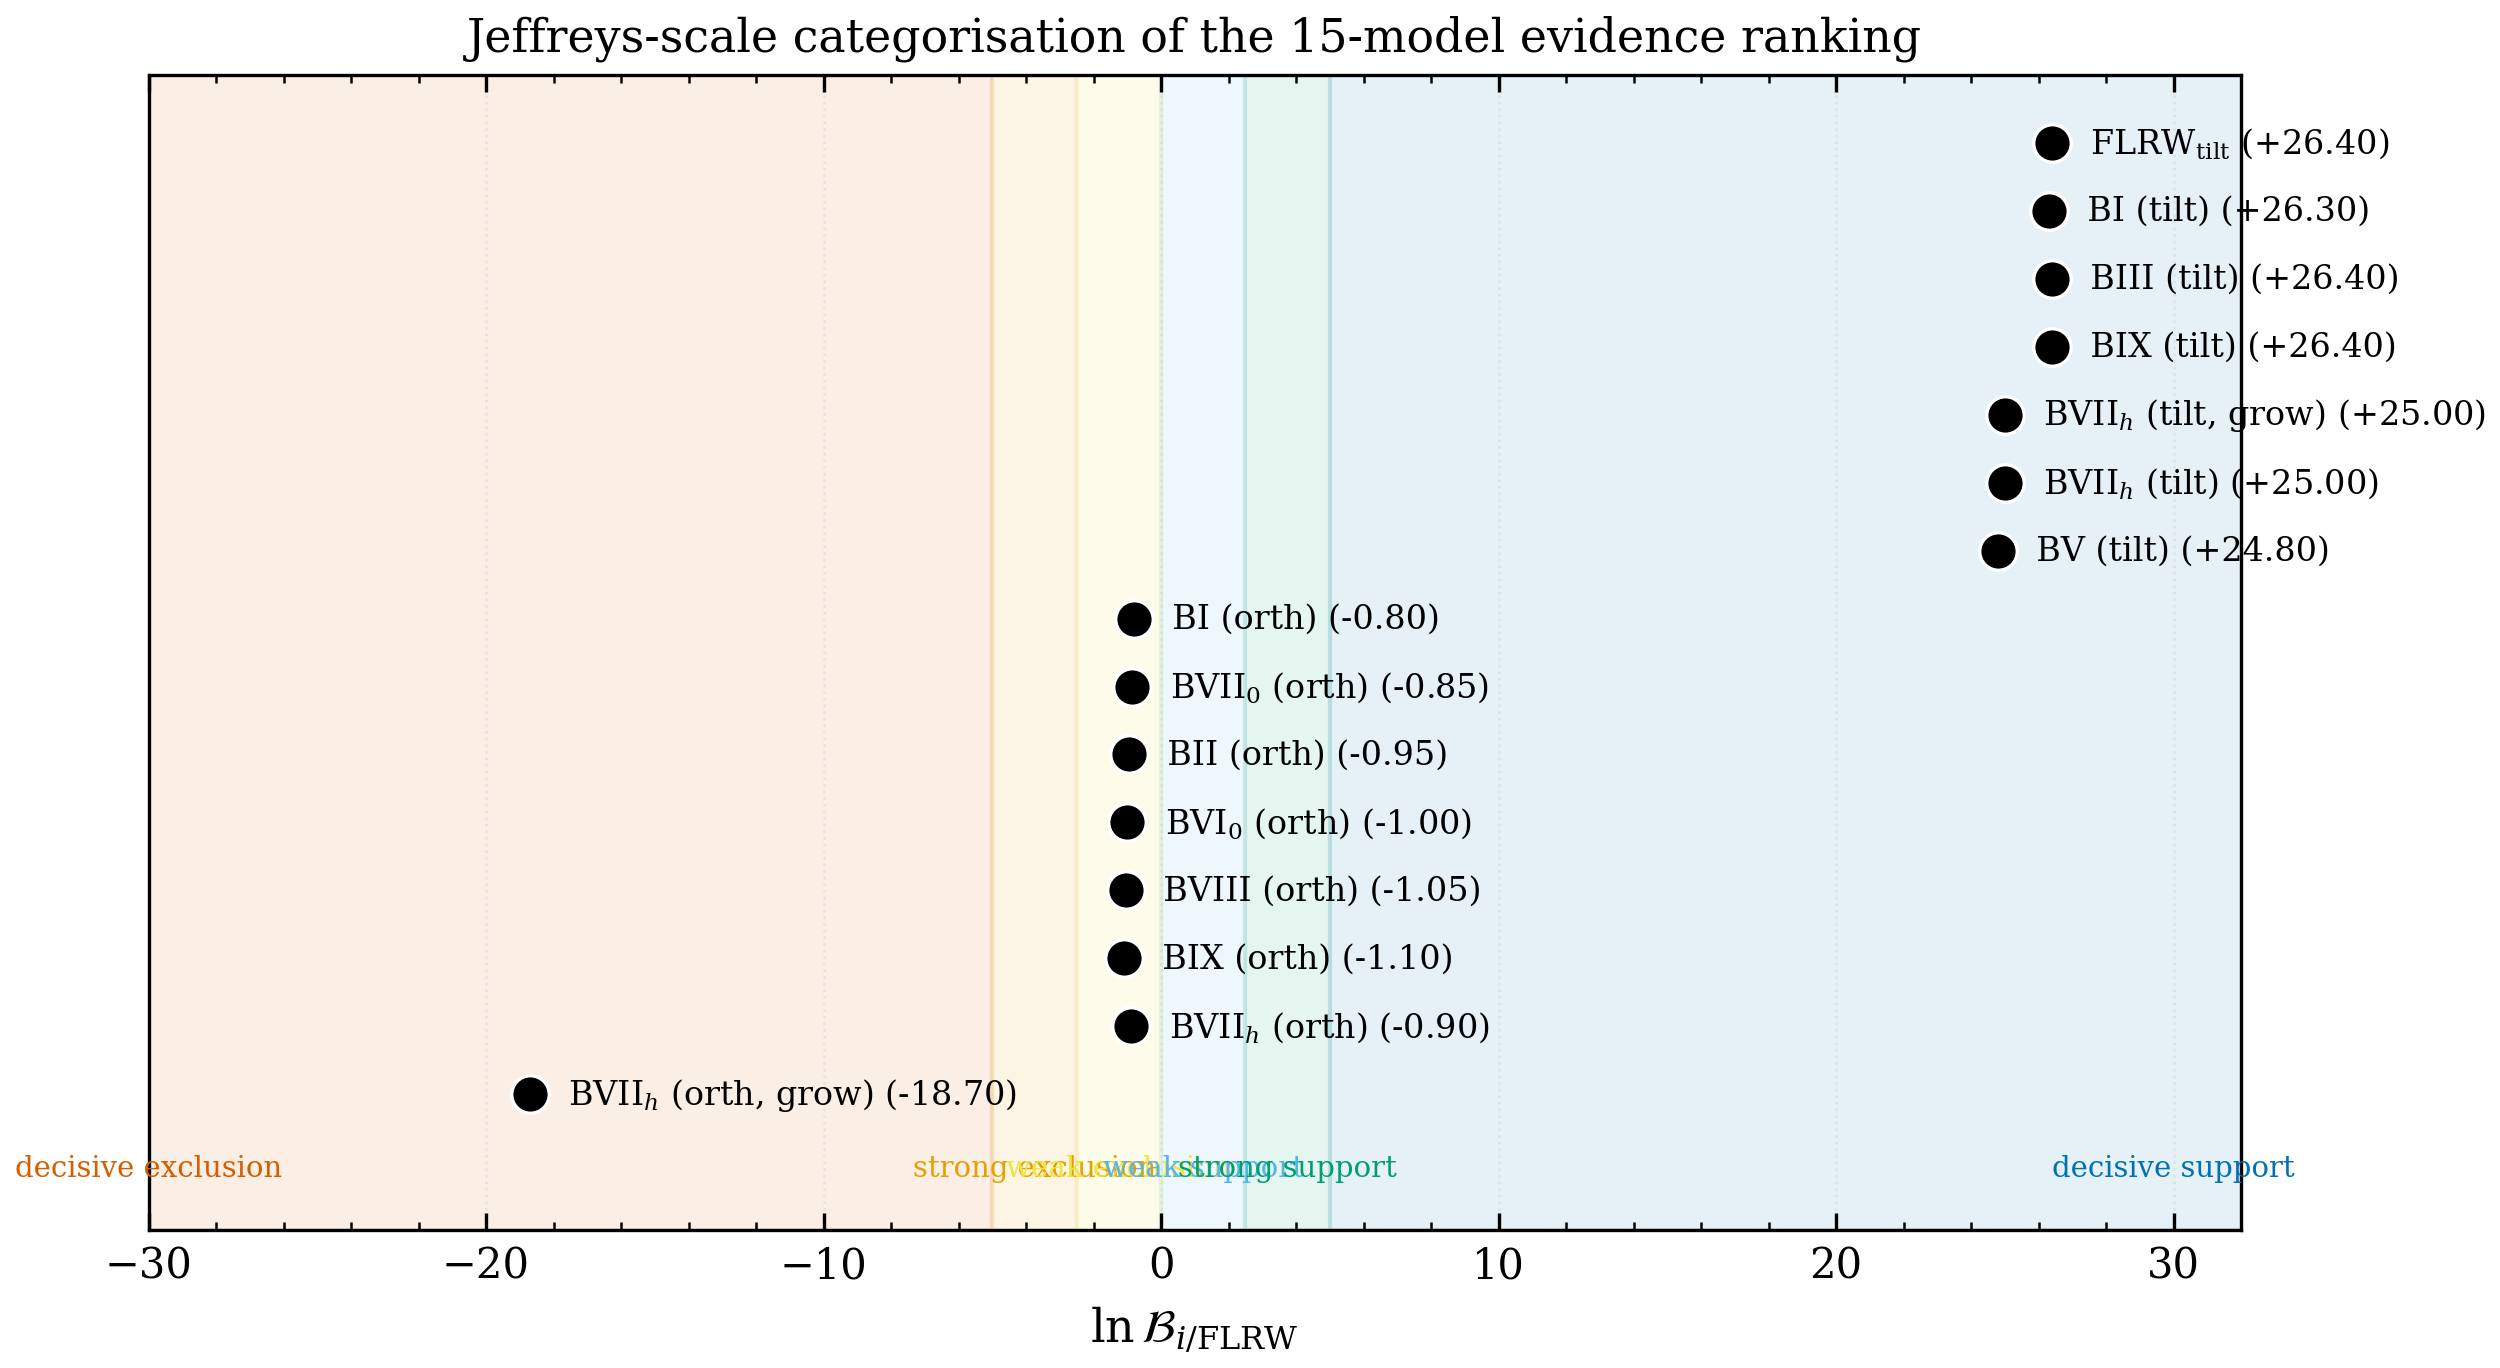
\includegraphics[width=0.82\textwidth,height=0.58\textheight,keepaspectratio]{conditioned_legacy/quarantined-legacy-root-sources__fig_jeffreys_categorization}
\captionof{figure}{Conditioned legacy diagnostic: jeffreys categorization. Condition: legacy manuscript-generator assumptions. See sidecar manifest for provenance and caveats; appendix-only, not native-transfer or family-ID evidence.}
\label{fig:conditioned-legacy-quarantined-legacy-root-sources-fig-jeffreys-categorization}
\end{center}

\clearpage
\begin{center}
\centering
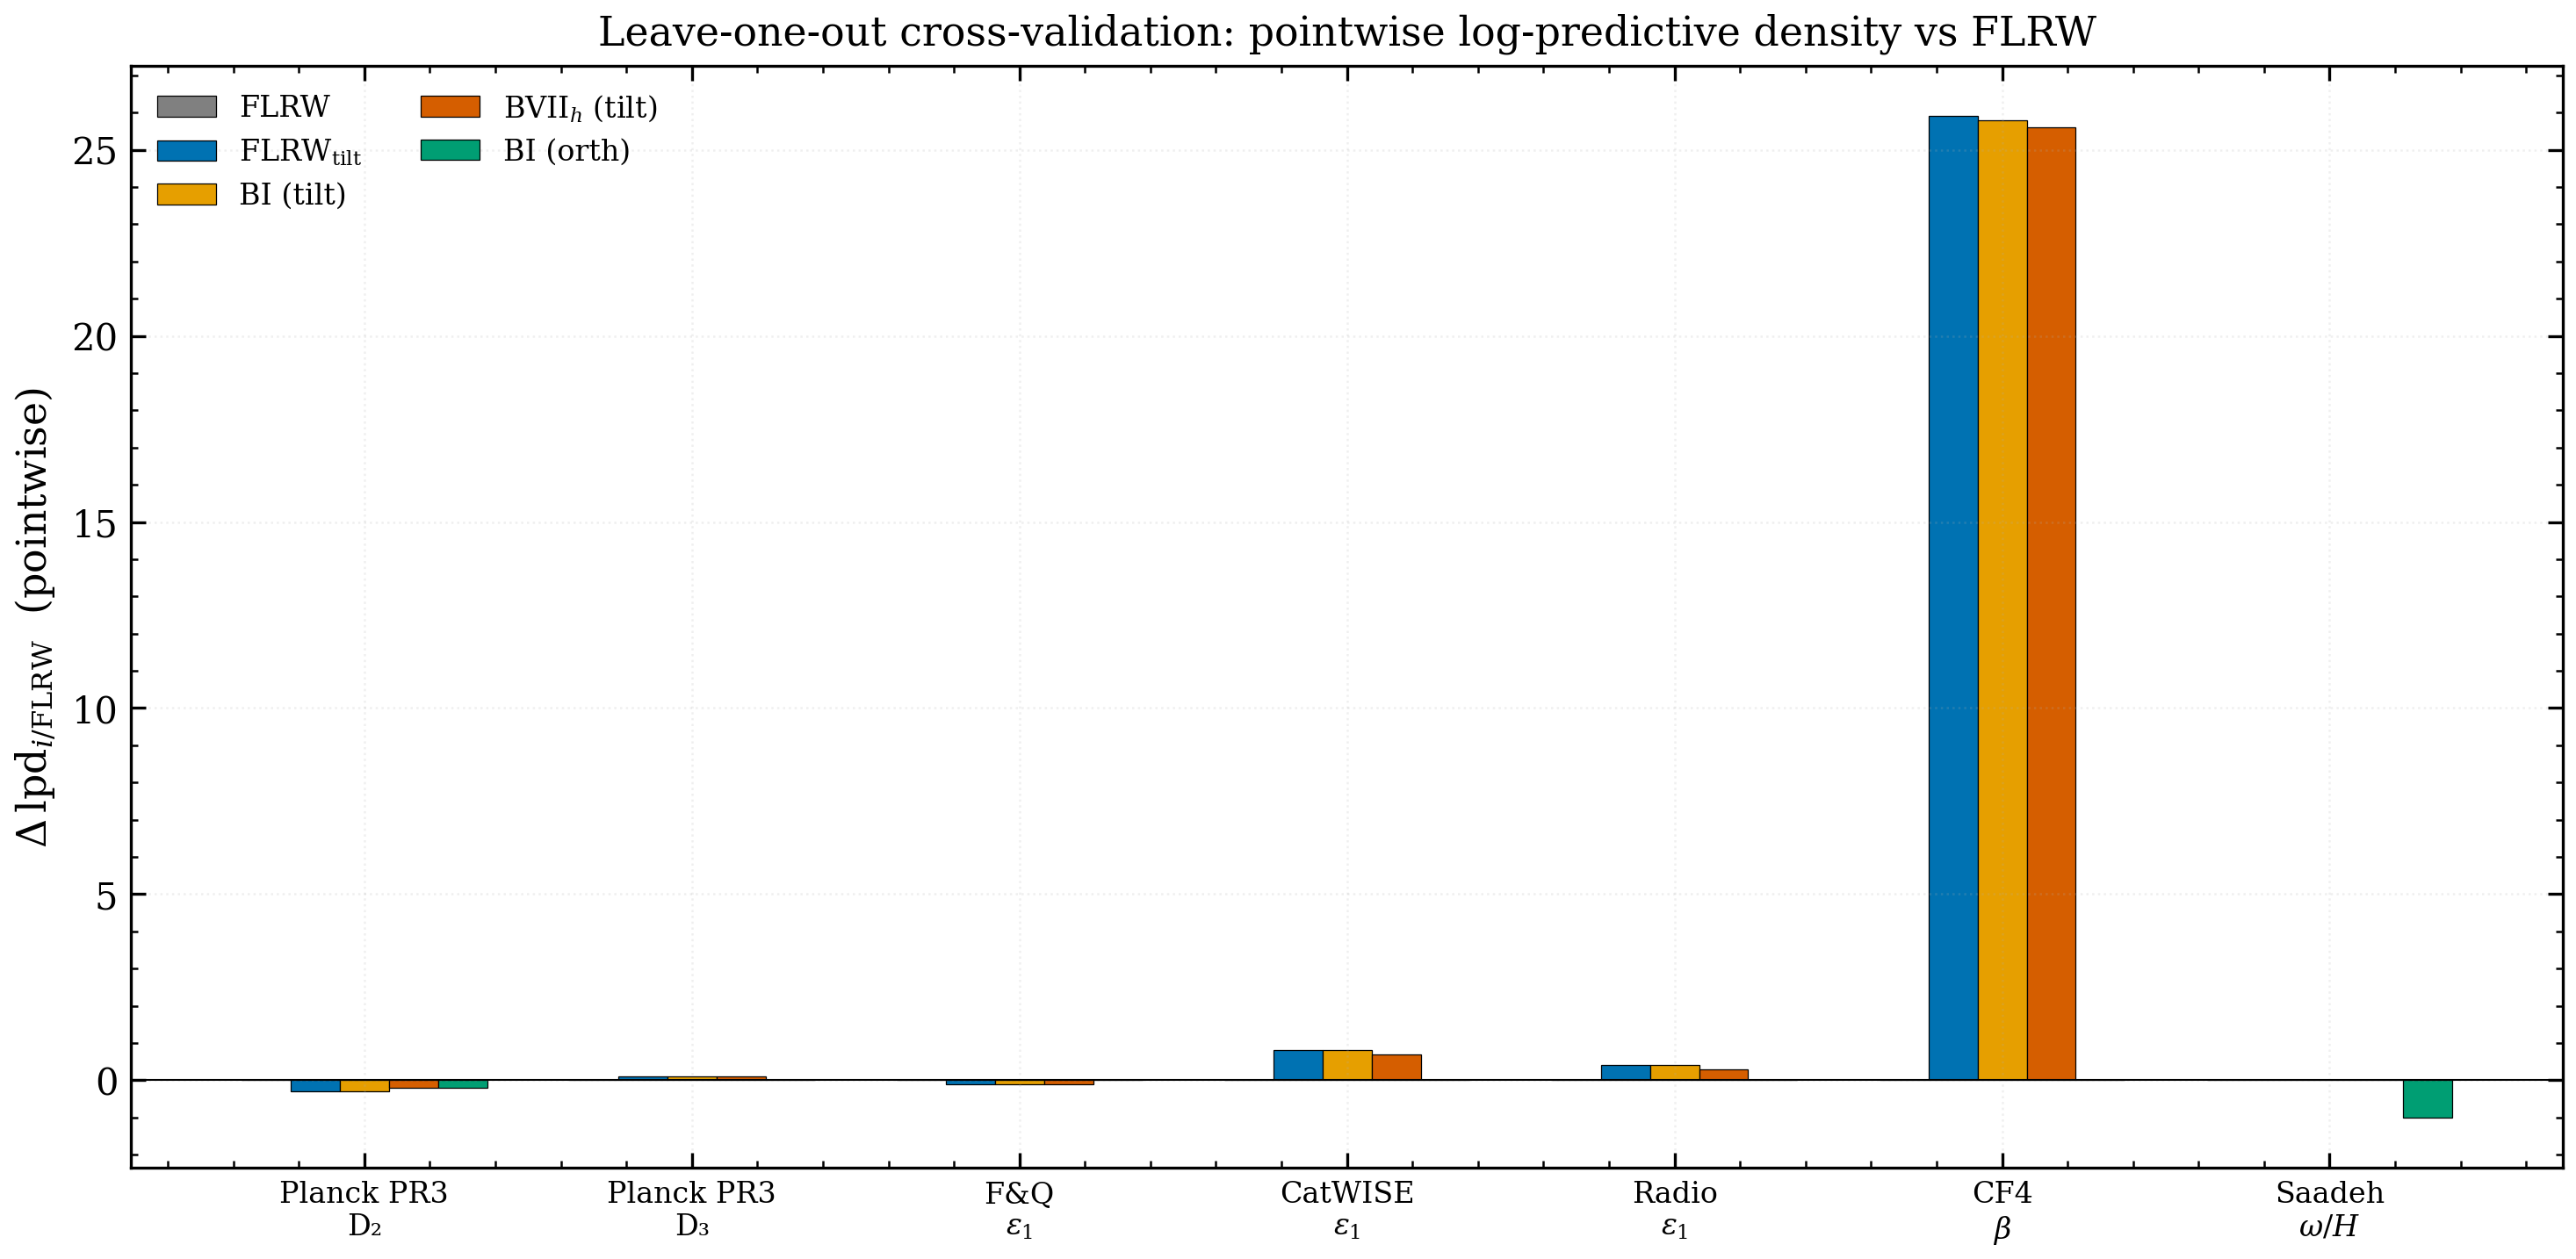
\includegraphics[width=0.82\textwidth,height=0.58\textheight,keepaspectratio]{conditioned_legacy/quarantined-legacy-root-sources__fig_leave_one_out}
\captionof{figure}{Conditioned legacy diagnostic: leave one out. Condition: legacy manuscript-generator assumptions. See sidecar manifest for provenance and caveats; appendix-only, not native-transfer or family-ID evidence.}
\label{fig:conditioned-legacy-quarantined-legacy-root-sources-fig-leave-one-out}
\end{center}

\clearpage
\begin{center}
\centering
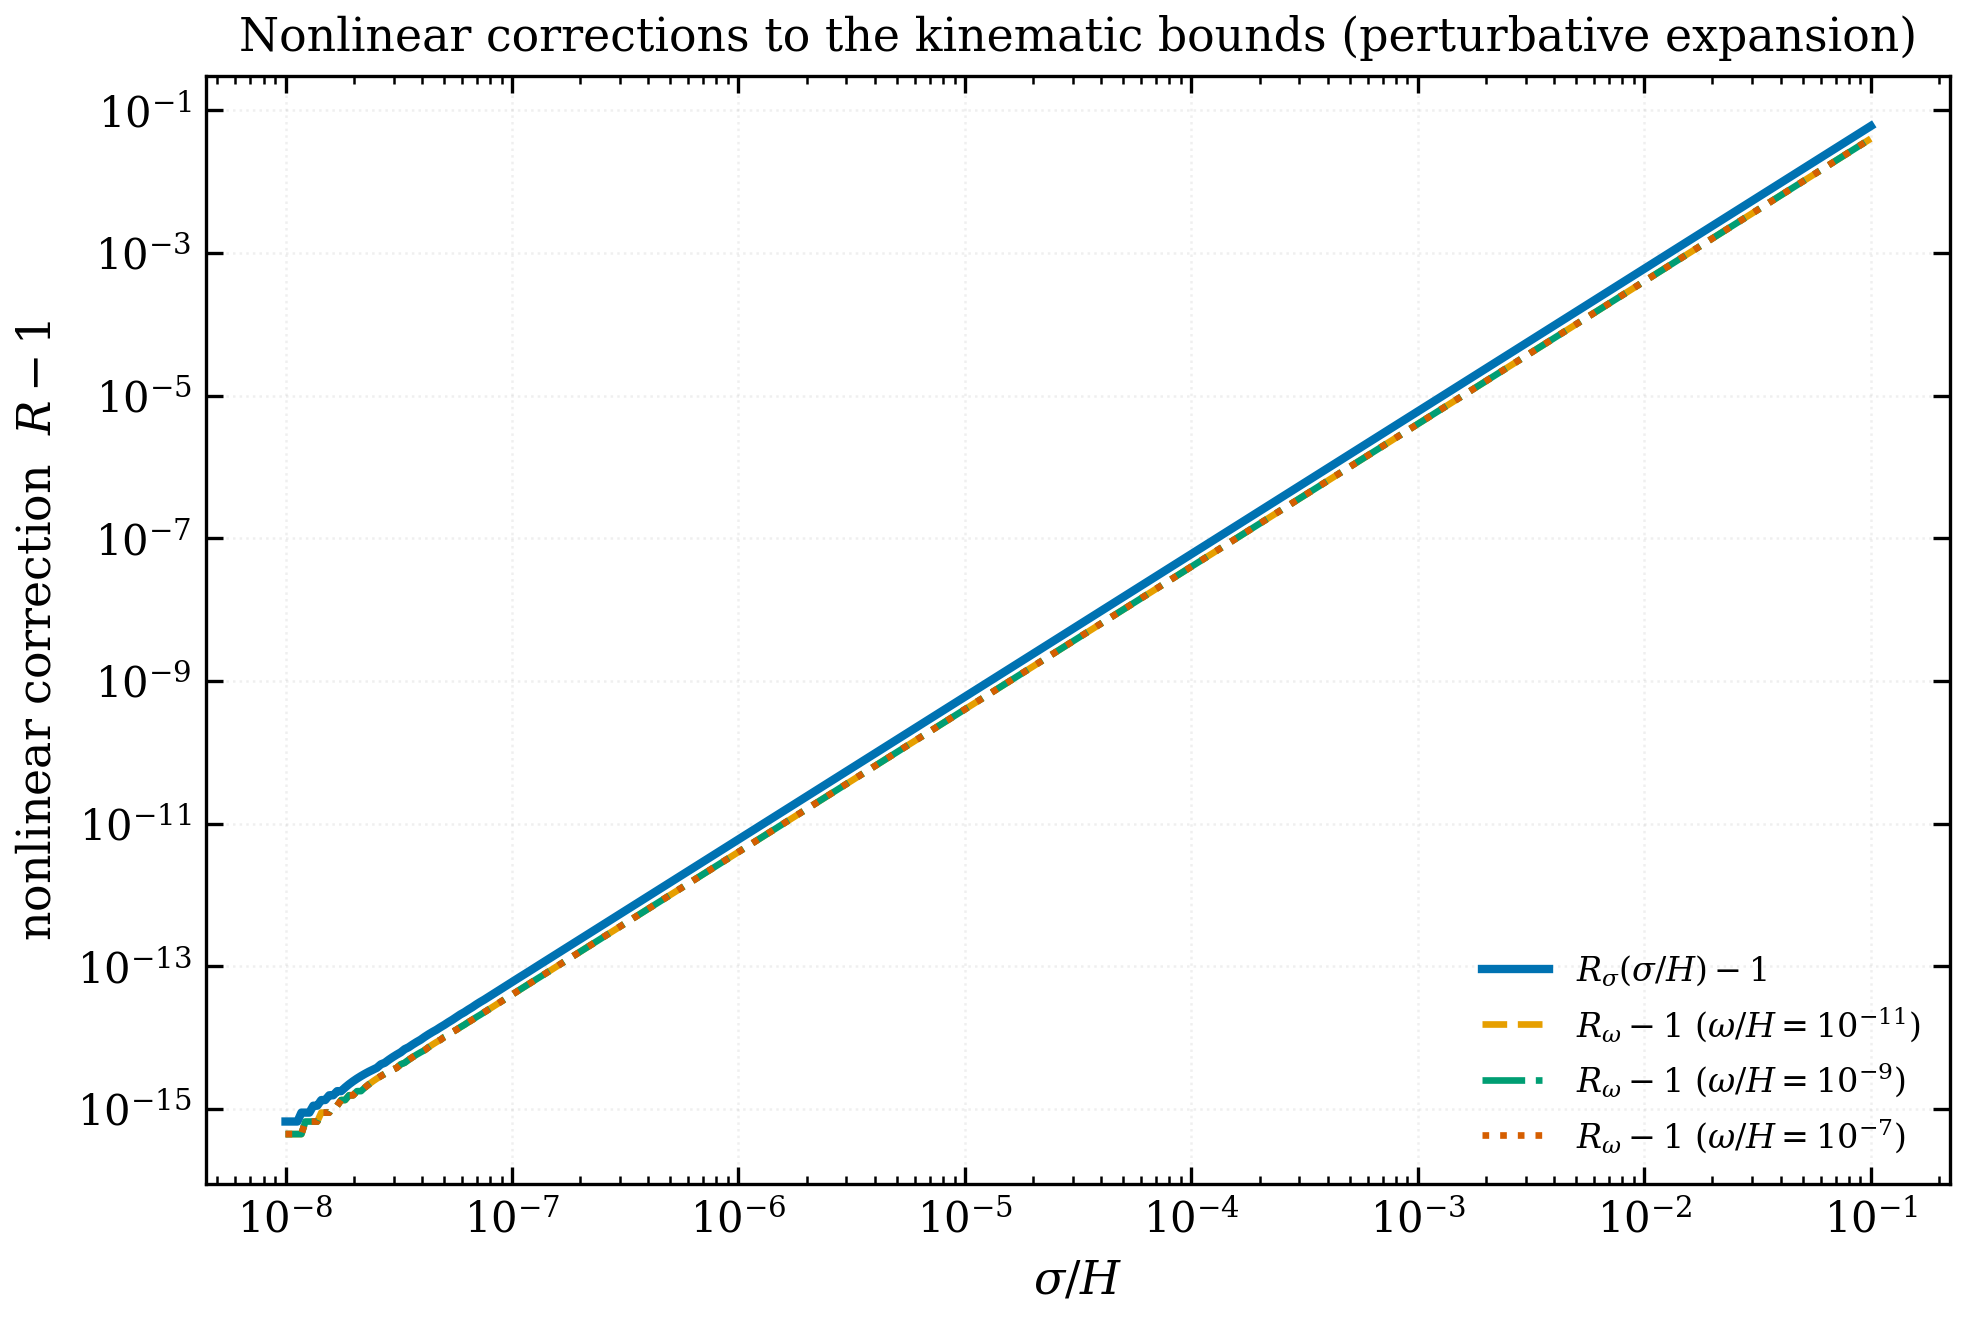
\includegraphics[width=0.82\textwidth,height=0.58\textheight,keepaspectratio]{conditioned_legacy/quarantined-legacy-root-sources__fig_nonlinear_corrections}
\captionof{figure}{Conditioned legacy diagnostic: nonlinear corrections. Condition: legacy manuscript-generator assumptions. See sidecar manifest for provenance and caveats; appendix-only, not native-transfer or family-ID evidence.}
\label{fig:conditioned-legacy-quarantined-legacy-root-sources-fig-nonlinear-corrections}
\end{center}

\clearpage
\begin{center}
\centering
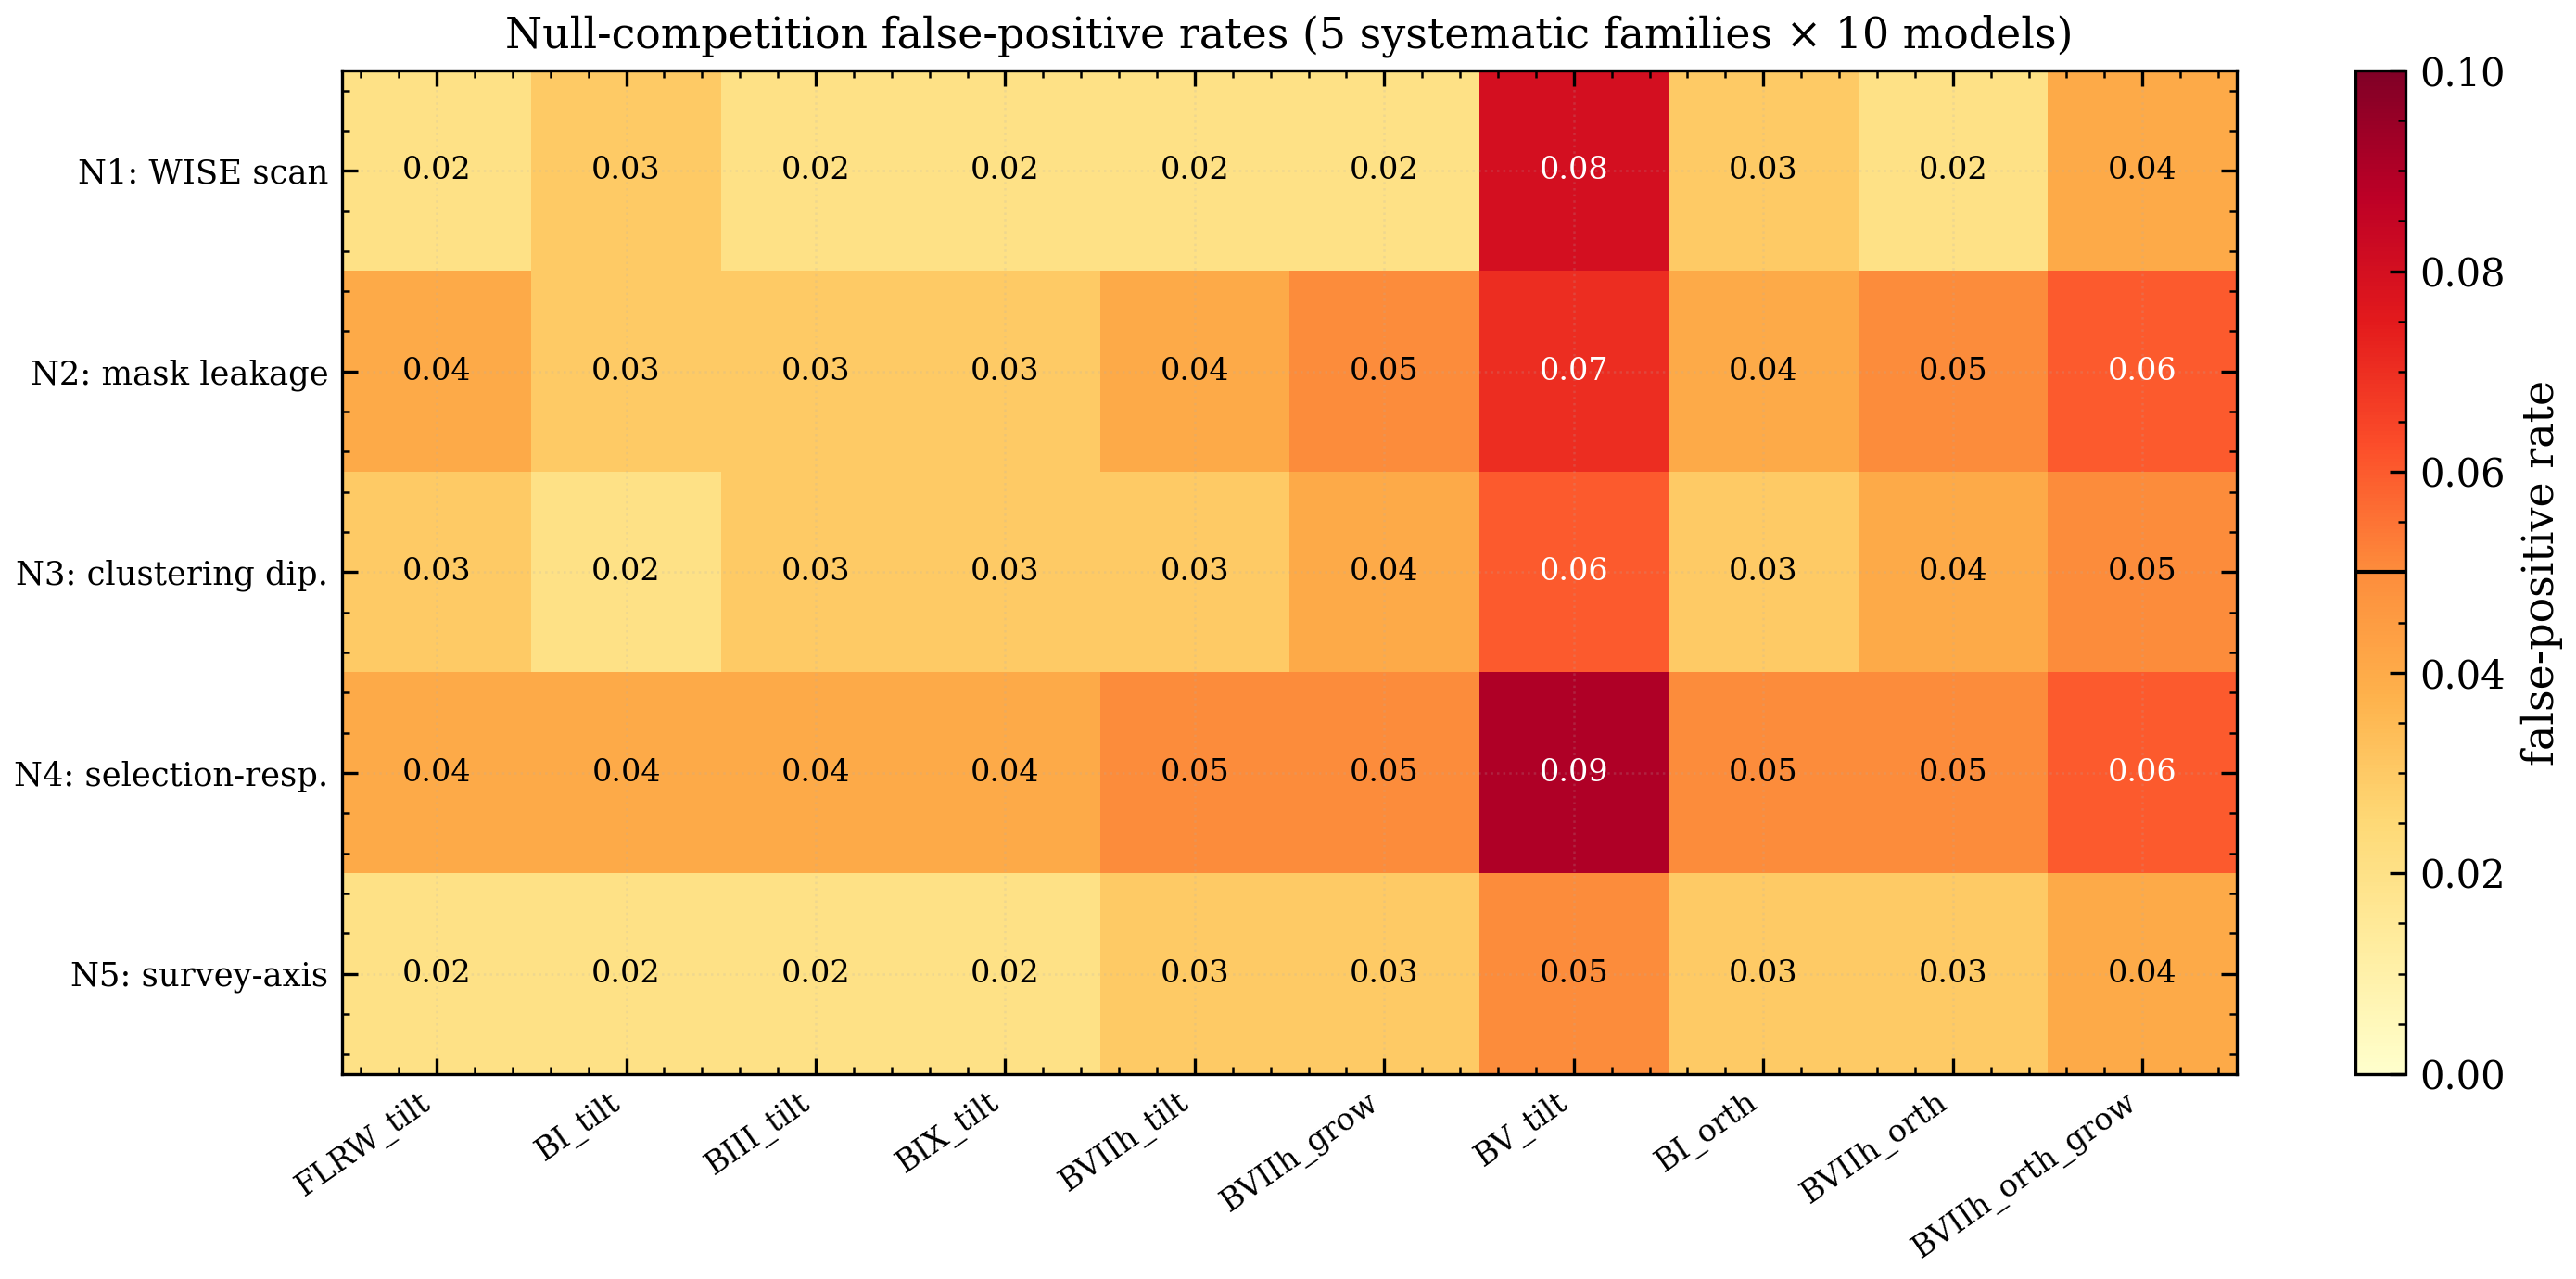
\includegraphics[width=0.82\textwidth,height=0.58\textheight,keepaspectratio]{conditioned_legacy/quarantined-legacy-root-sources__fig_null_competition_production}
\captionof{figure}{Conditioned legacy diagnostic: null competition production. Condition: legacy manuscript-generator assumptions. See sidecar manifest for provenance and caveats; appendix-only, not native-transfer or family-ID evidence.}
\label{fig:conditioned-legacy-quarantined-legacy-root-sources-fig-null-competition-production}
\end{center}

\clearpage
\begin{center}
\centering
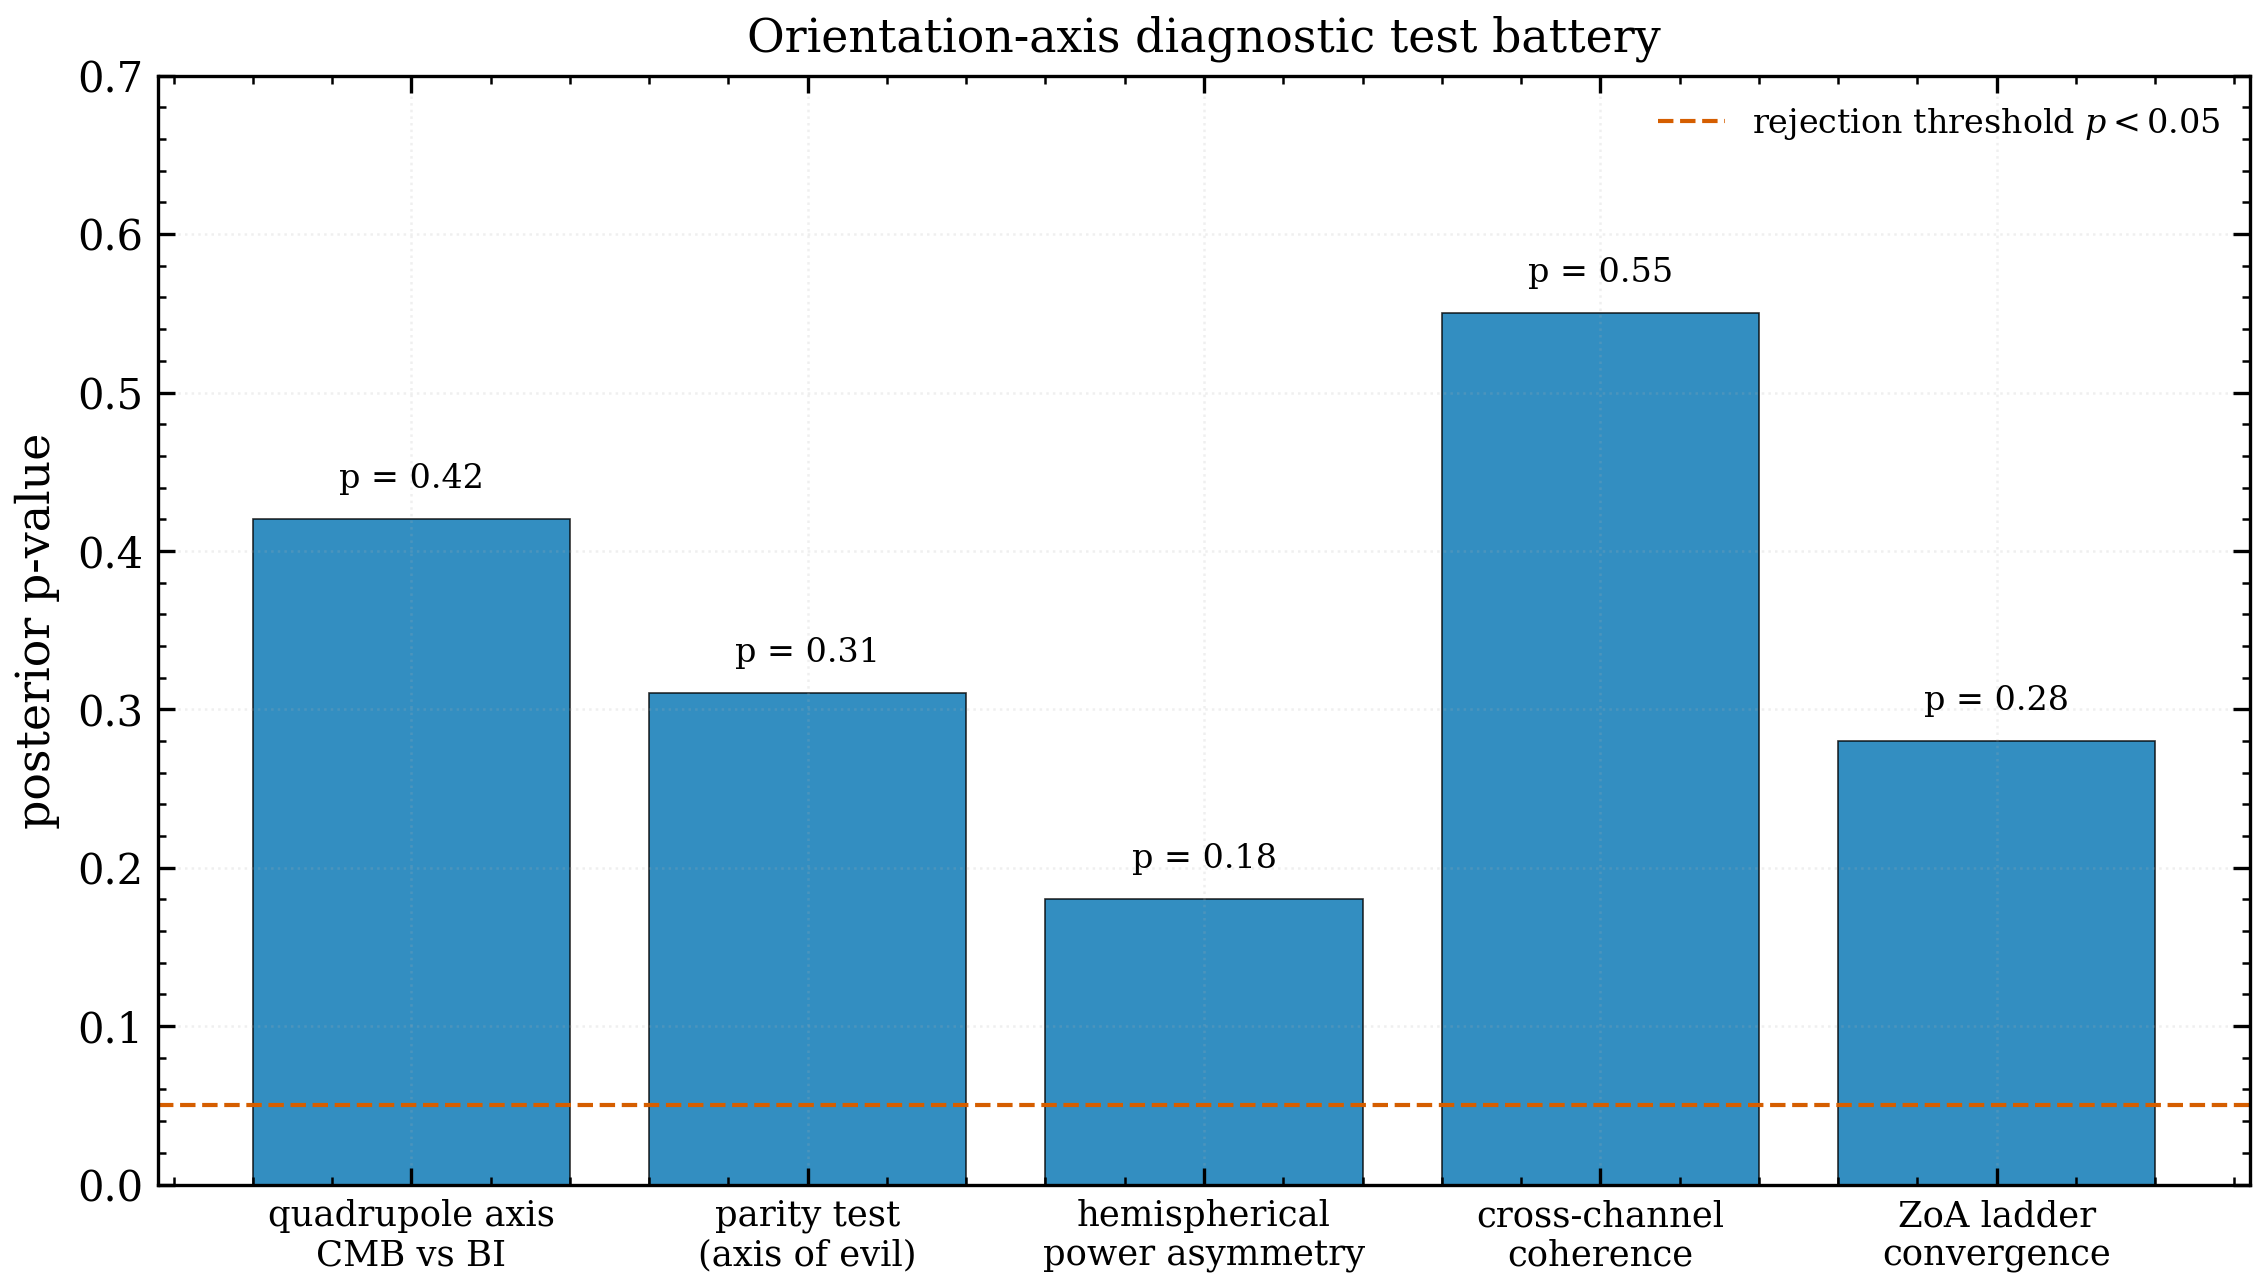
\includegraphics[width=0.82\textwidth,height=0.58\textheight,keepaspectratio]{conditioned_legacy/quarantined-legacy-root-sources__fig_orientation_diagnostics}
\captionof{figure}{Conditioned legacy diagnostic: orientation diagnostics. Condition: legacy manuscript-generator assumptions. See sidecar manifest for provenance and caveats; appendix-only, not native-transfer or family-ID evidence.}
\label{fig:conditioned-legacy-quarantined-legacy-root-sources-fig-orientation-diagnostics}
\end{center}

\clearpage
\begin{center}
\centering
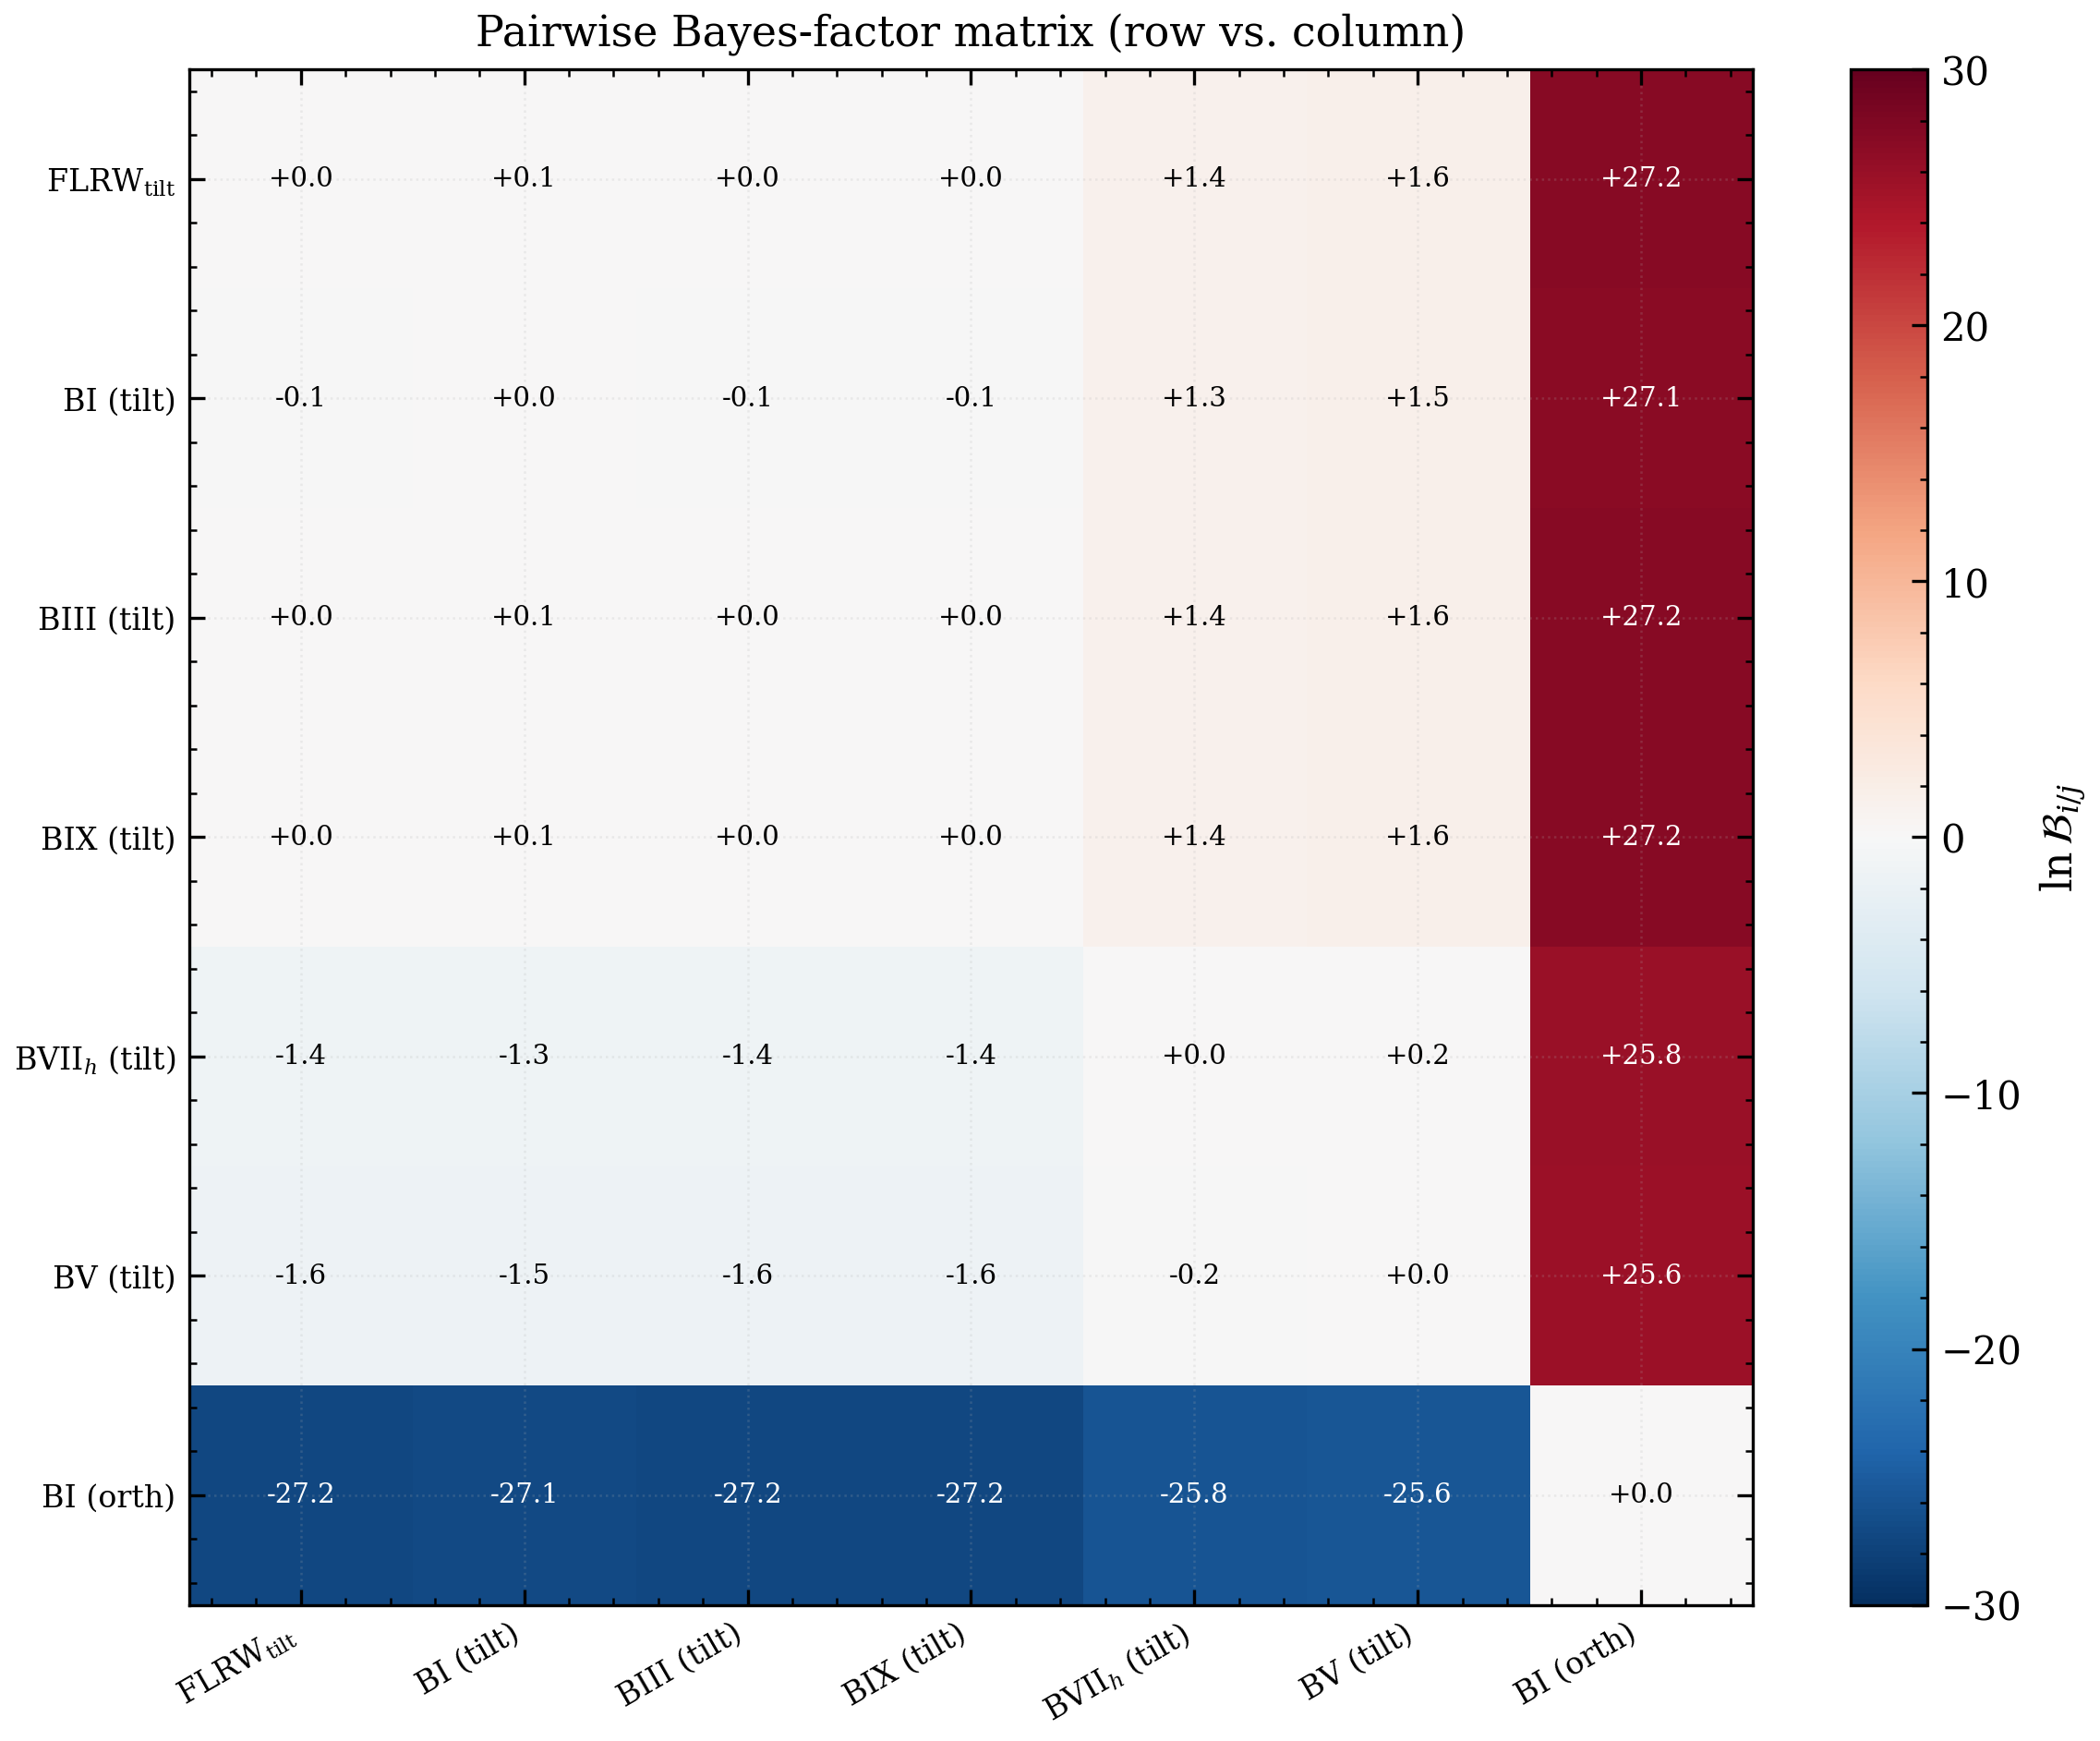
\includegraphics[width=0.82\textwidth,height=0.58\textheight,keepaspectratio]{conditioned_legacy/quarantined-legacy-root-sources__fig_pairwise_bf_matrix}
\captionof{figure}{Conditioned legacy diagnostic: pairwise bf matrix. Condition: legacy statistical assumptions without current null/PPC/LOOCV refresh. See sidecar manifest for provenance and caveats; appendix-only, not native-transfer or family-ID evidence.}
\label{fig:conditioned-legacy-quarantined-legacy-root-sources-fig-pairwise-bf-matrix}
\end{center}

\clearpage
\begin{center}
\centering
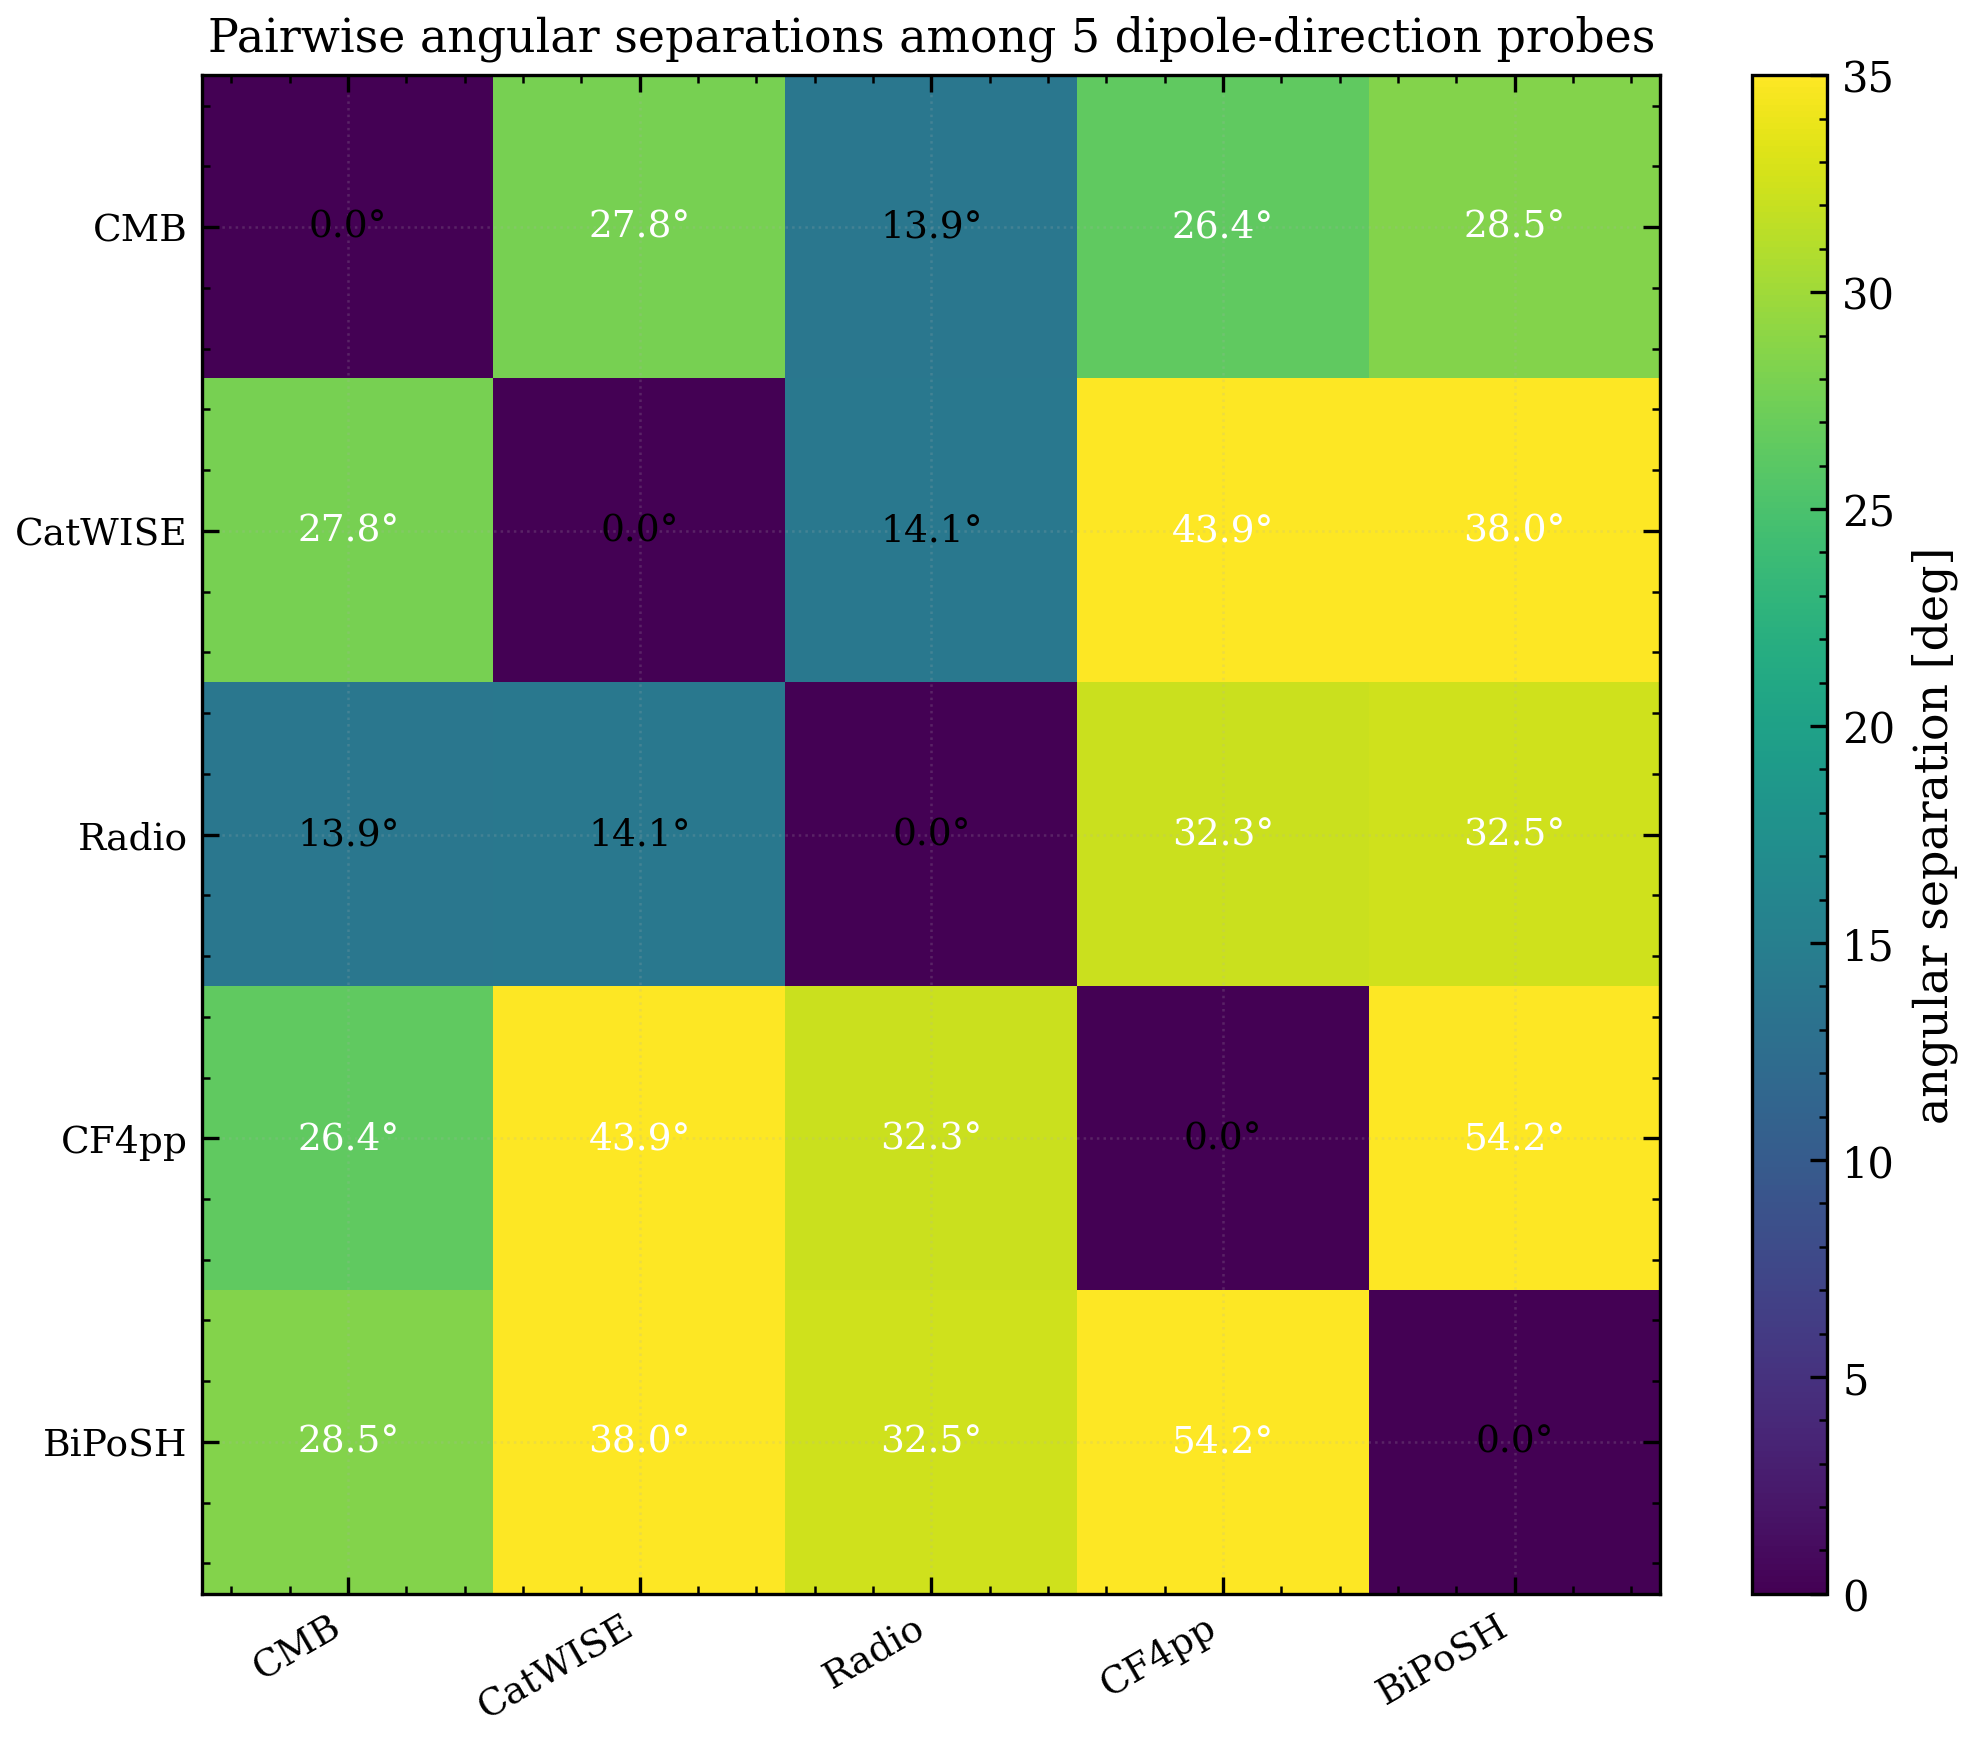
\includegraphics[width=0.82\textwidth,height=0.58\textheight,keepaspectratio]{conditioned_legacy/quarantined-legacy-root-sources__fig_pairwise_separations_matrix}
\captionof{figure}{Conditioned legacy diagnostic: pairwise separations matrix. Condition: legacy manuscript-generator assumptions. See sidecar manifest for provenance and caveats; appendix-only, not native-transfer or family-ID evidence.}
\label{fig:conditioned-legacy-quarantined-legacy-root-sources-fig-pairwise-separations-matrix}
\end{center}

\clearpage
\begin{center}
\centering
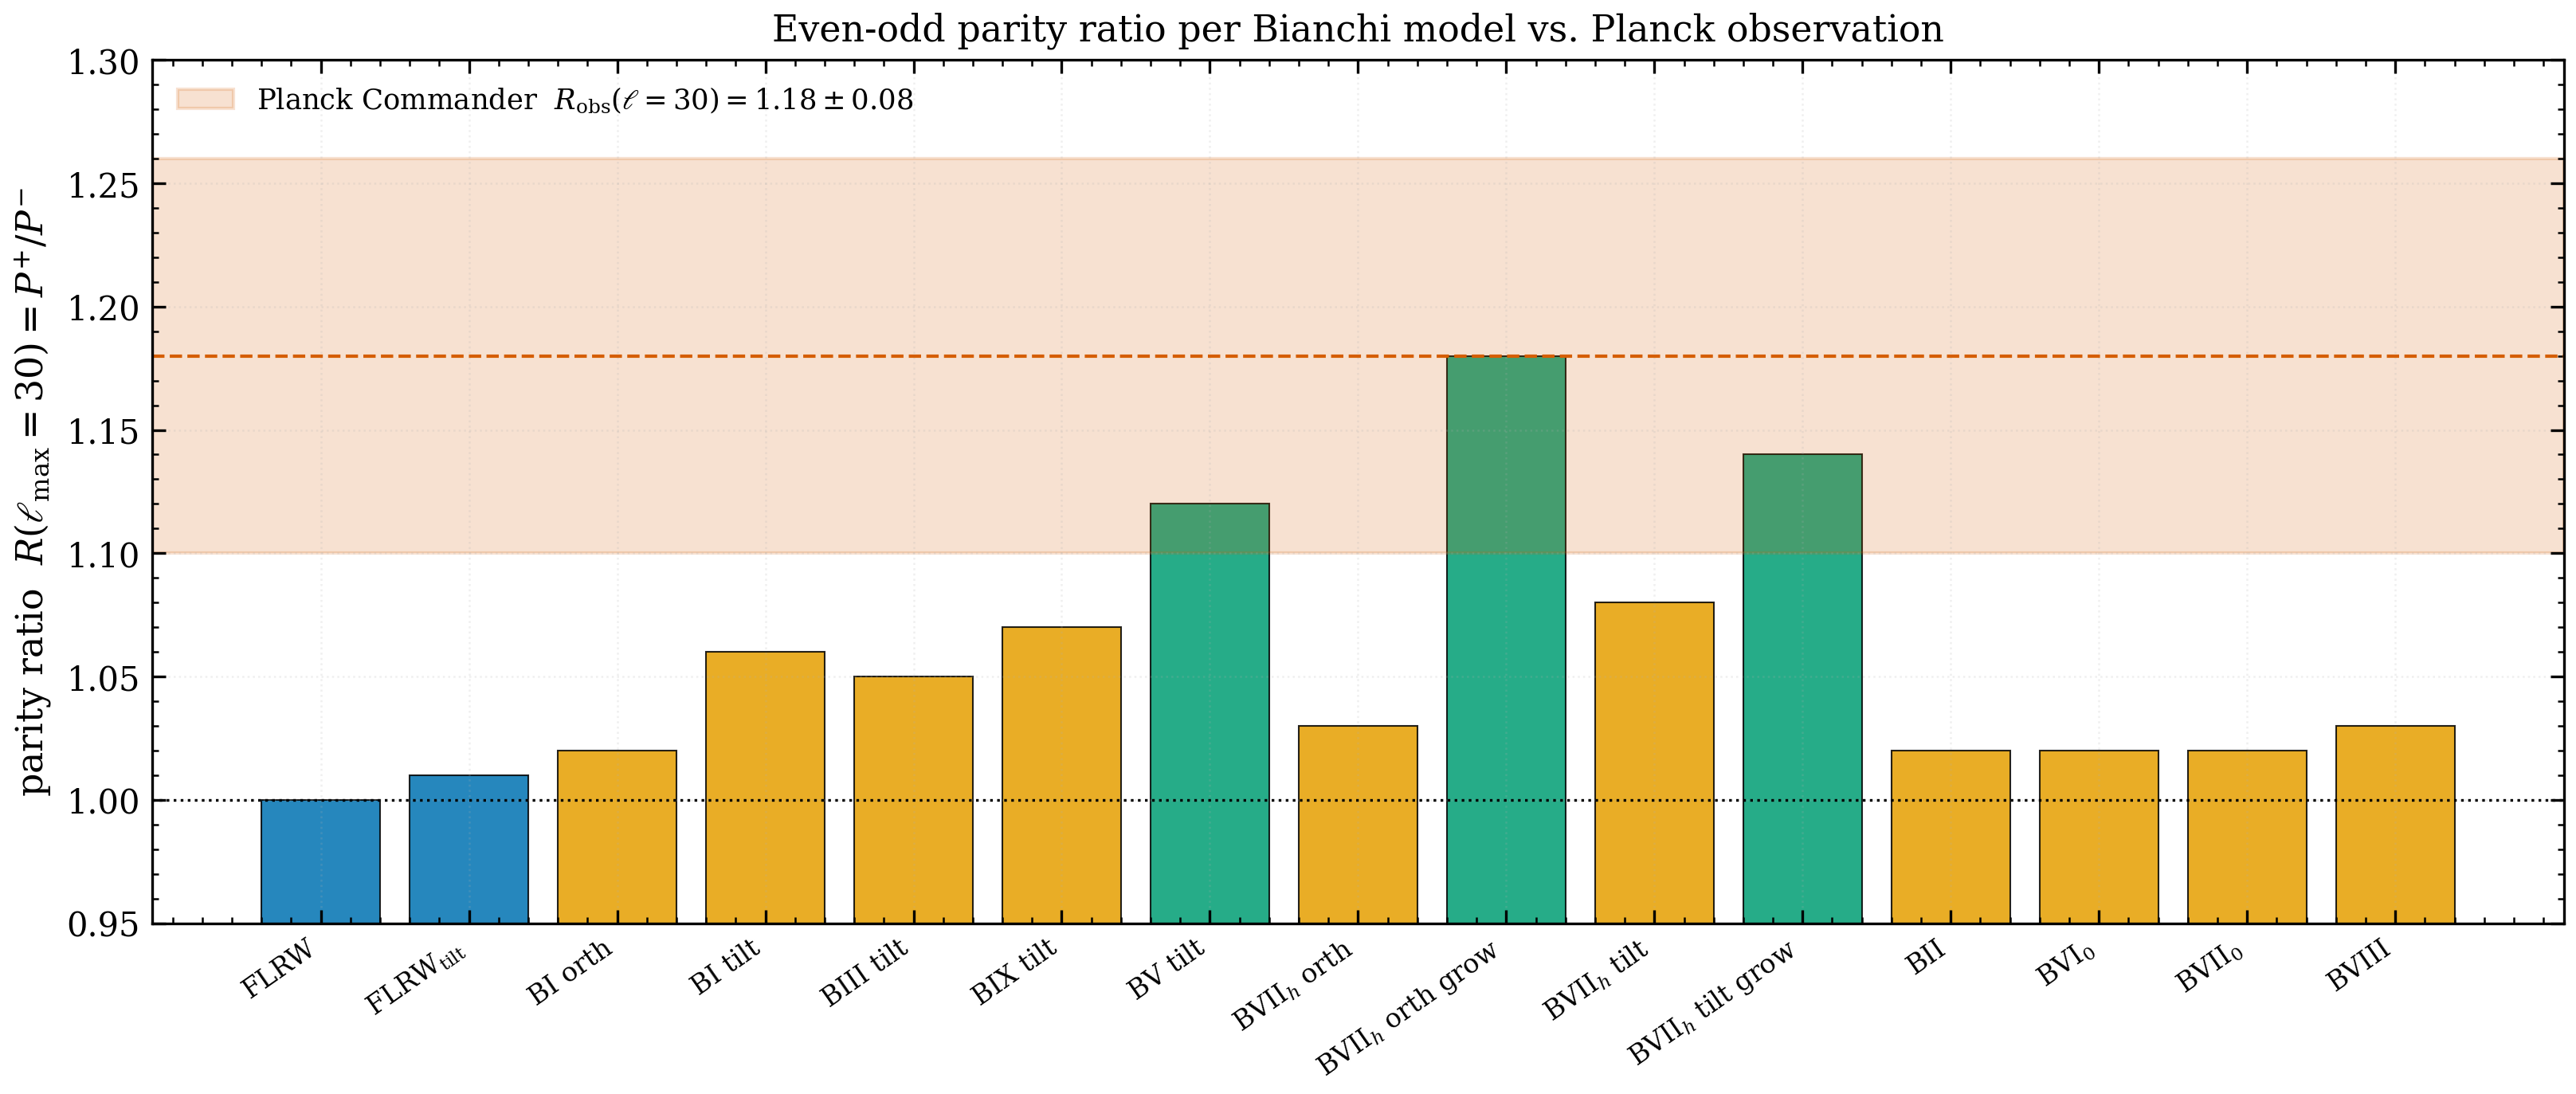
\includegraphics[width=0.82\textwidth,height=0.58\textheight,keepaspectratio]{conditioned_legacy/quarantined-legacy-root-sources__fig_parity_asymmetry_per_model}
\captionof{figure}{Conditioned legacy diagnostic: parity asymmetry per model. Condition: legacy manuscript-generator assumptions. See sidecar manifest for provenance and caveats; appendix-only, not native-transfer or family-ID evidence.}
\label{fig:conditioned-legacy-quarantined-legacy-root-sources-fig-parity-asymmetry-per-model}
\end{center}

\clearpage
\begin{center}
\centering
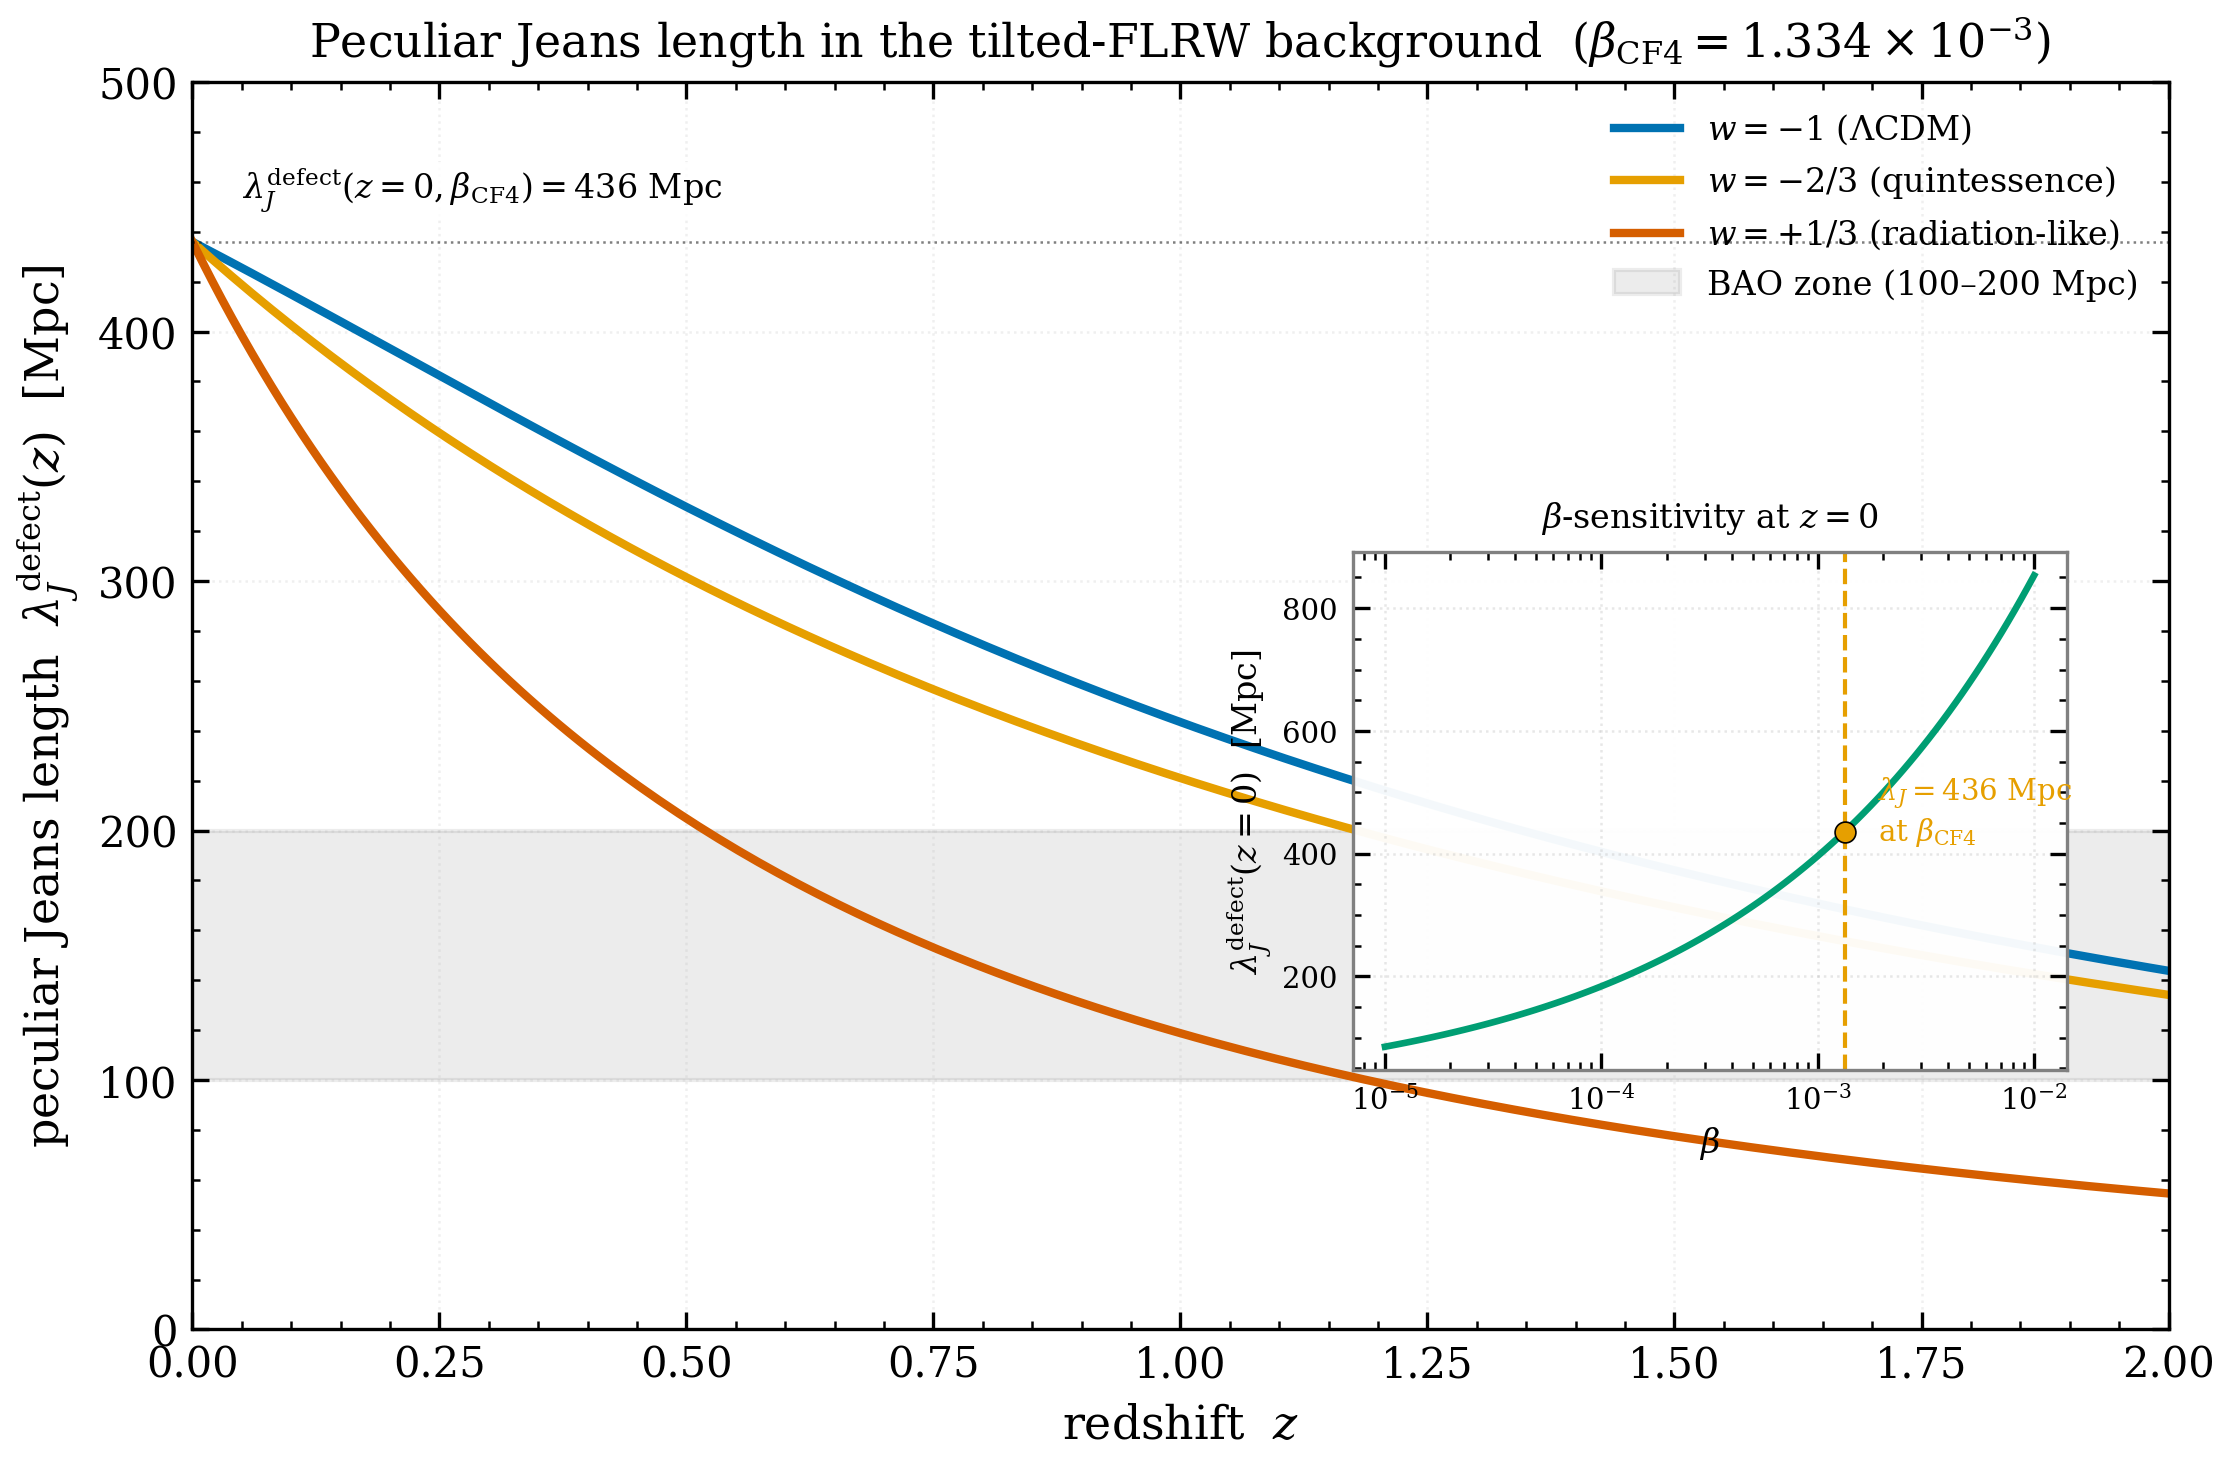
\includegraphics[width=0.82\textwidth,height=0.58\textheight,keepaspectratio]{conditioned_legacy/quarantined-legacy-root-sources__fig_peculiar_jeans}
\captionof{figure}{Conditioned legacy diagnostic: peculiar jeans. Condition: legacy manuscript-generator assumptions. See sidecar manifest for provenance and caveats; appendix-only, not native-transfer or family-ID evidence.}
\label{fig:conditioned-legacy-quarantined-legacy-root-sources-fig-peculiar-jeans}
\end{center}

\clearpage
\begin{center}
\centering
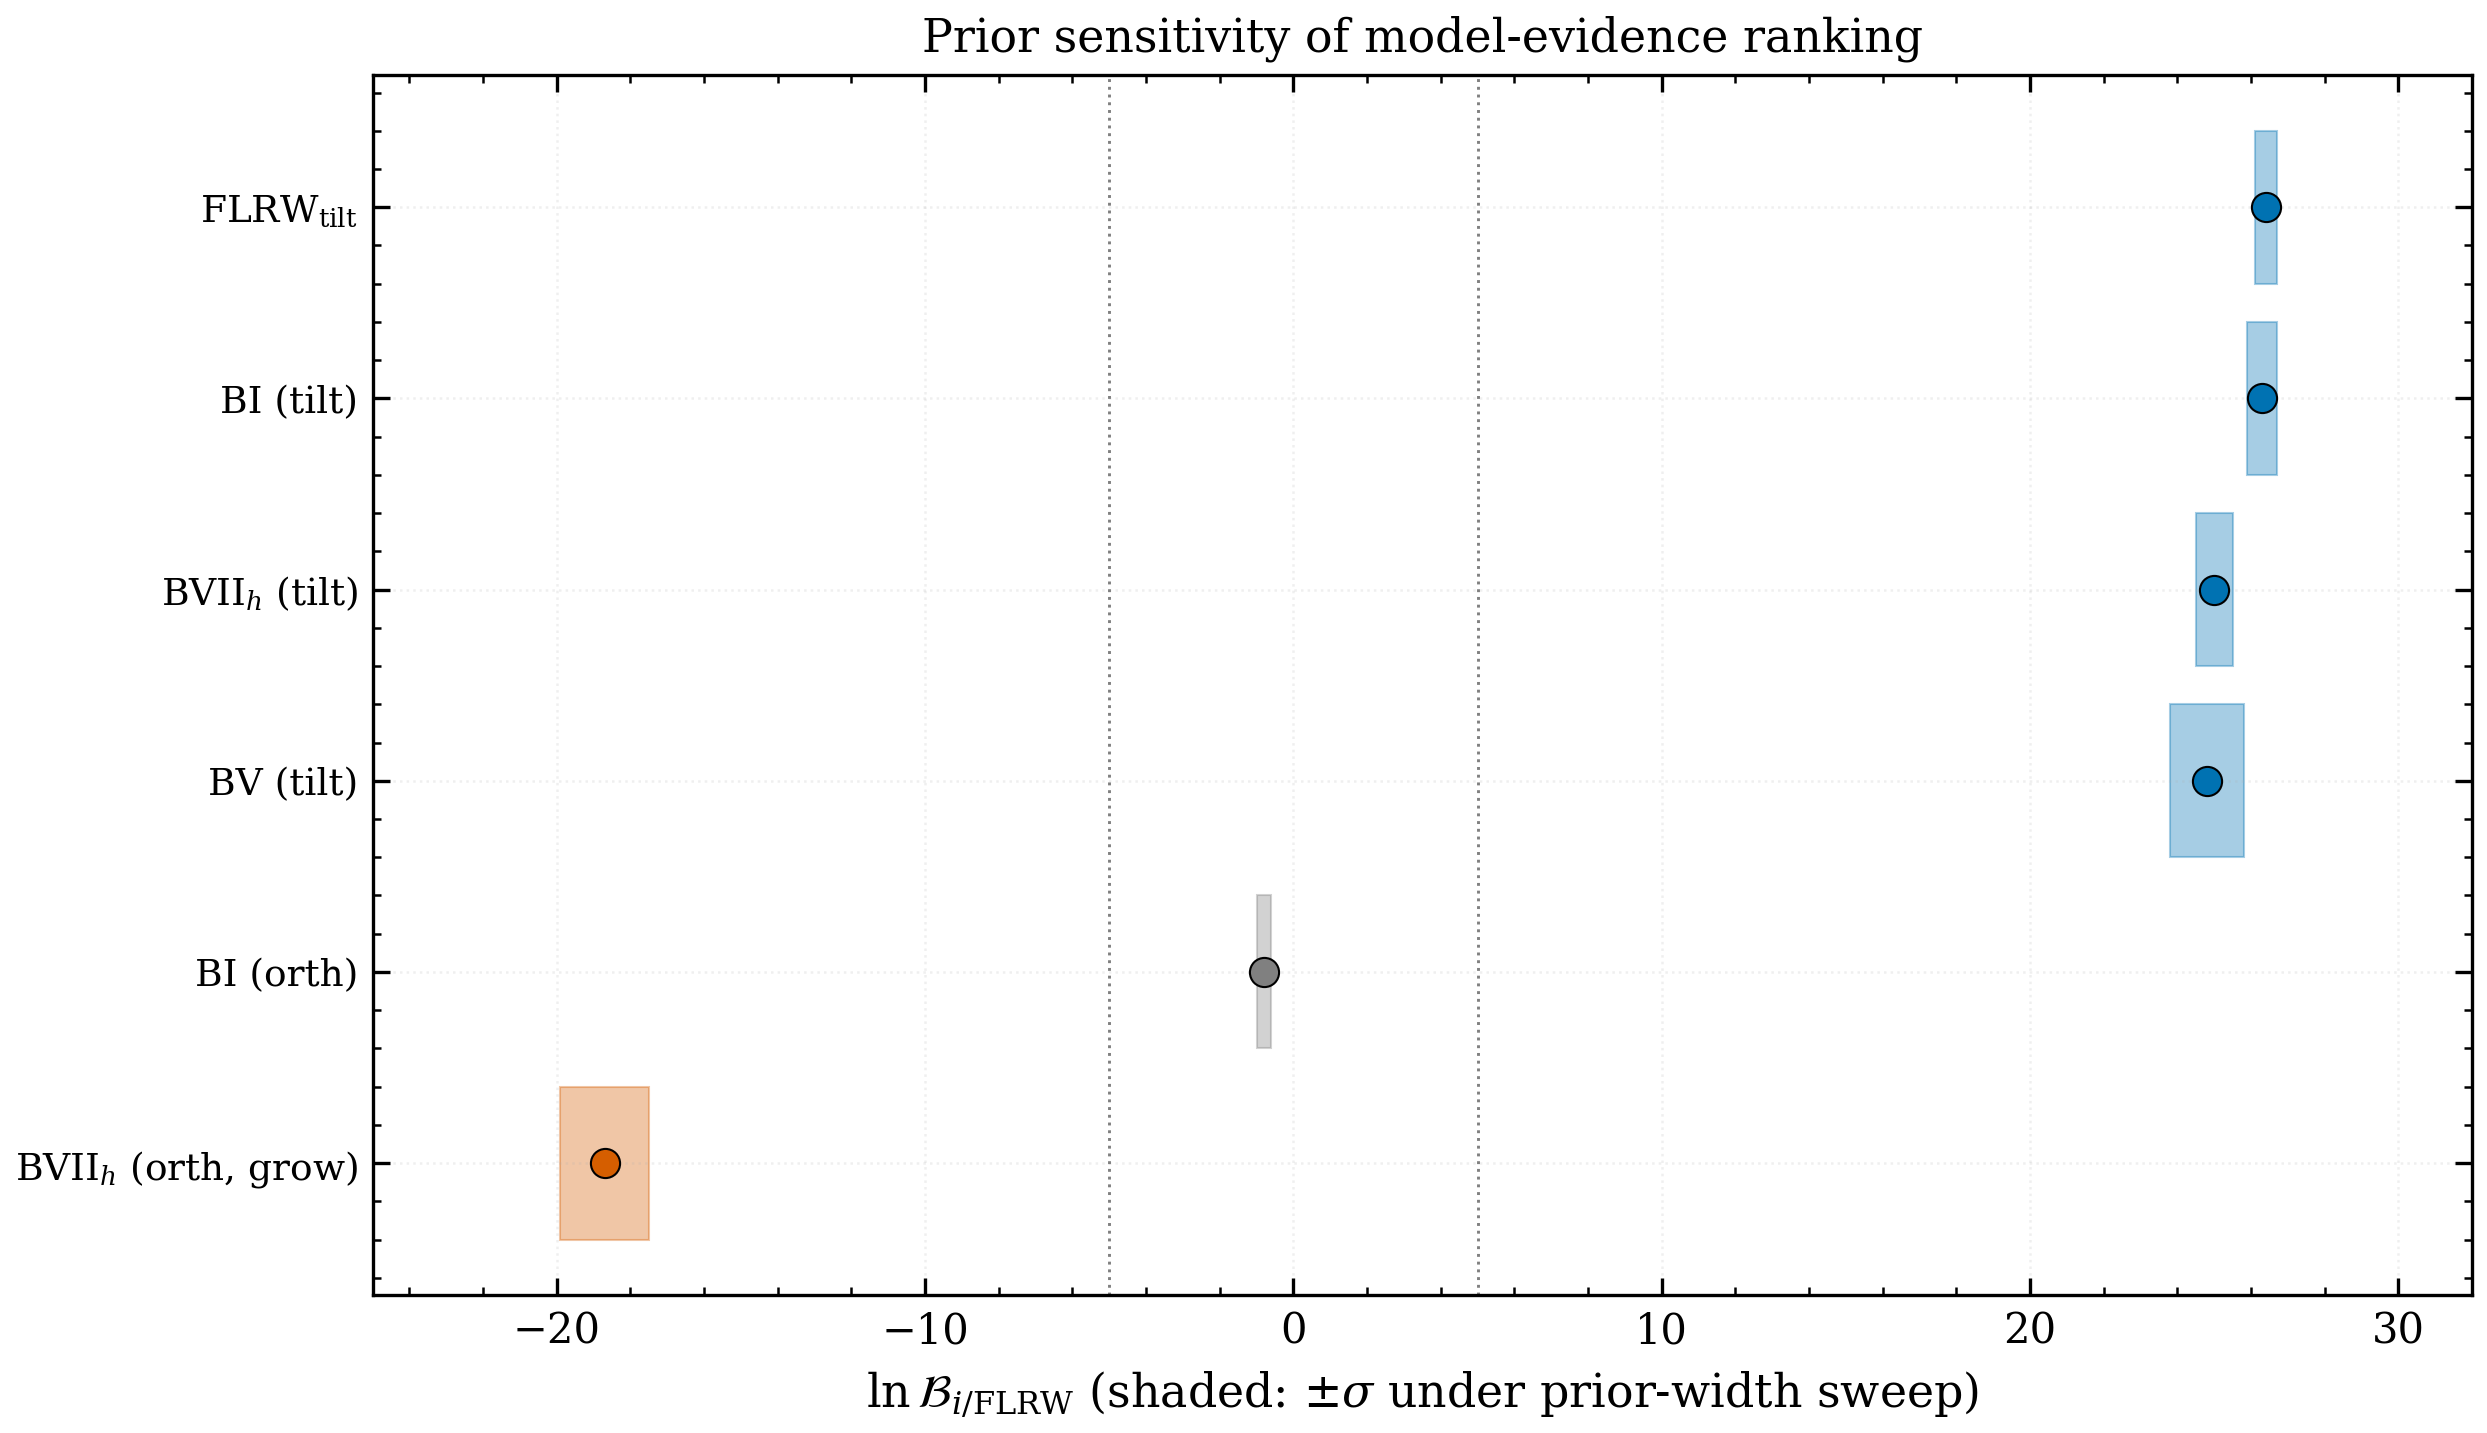
\includegraphics[width=0.82\textwidth,height=0.58\textheight,keepaspectratio]{conditioned_legacy/quarantined-legacy-root-sources__fig_prior_sensitivity}
\captionof{figure}{Conditioned legacy diagnostic: prior sensitivity. Condition: legacy manuscript-generator assumptions. See sidecar manifest for provenance and caveats; appendix-only, not native-transfer or family-ID evidence.}
\label{fig:conditioned-legacy-quarantined-legacy-root-sources-fig-prior-sensitivity}
\end{center}

\clearpage
\begin{center}
\centering
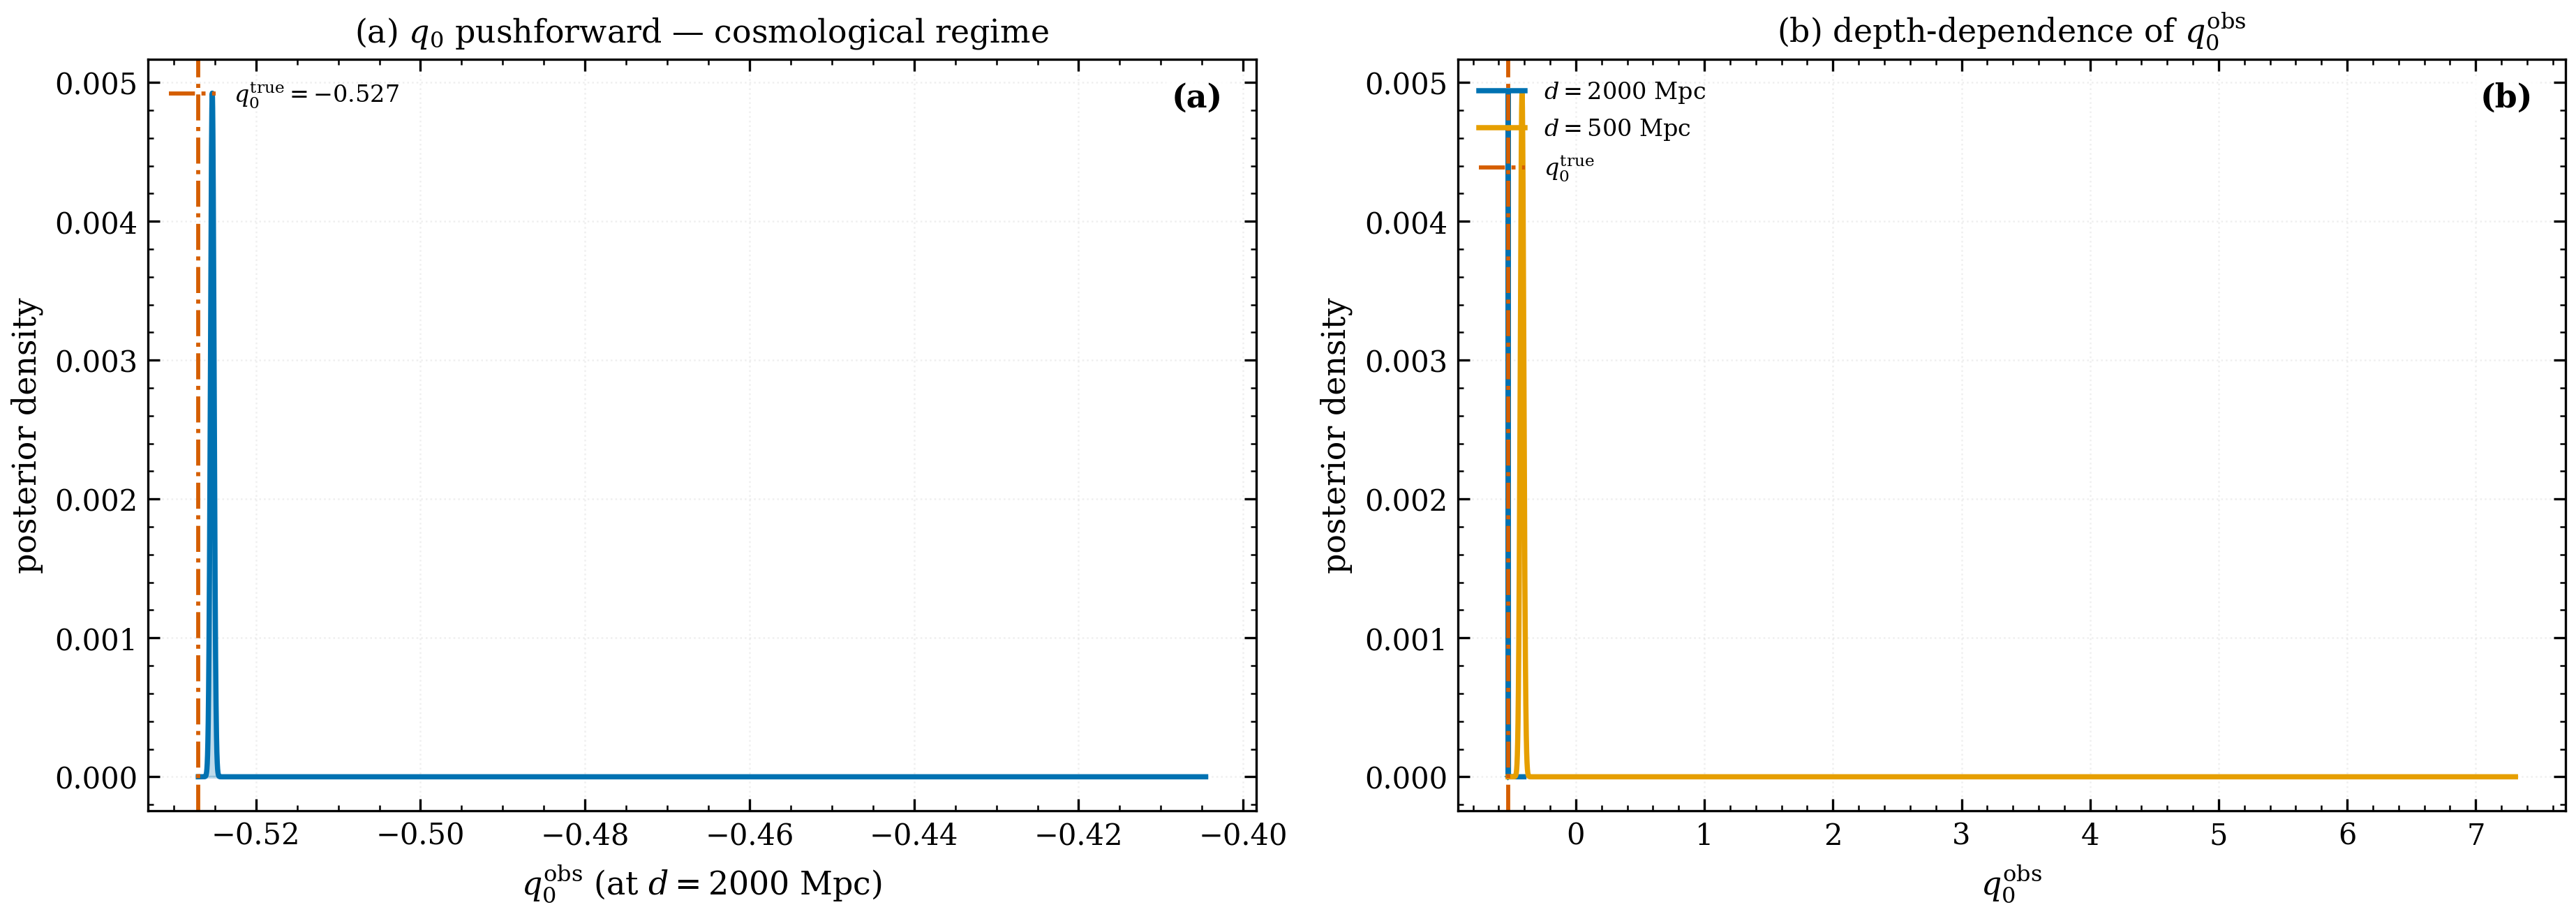
\includegraphics[width=0.82\textwidth,height=0.58\textheight,keepaspectratio]{conditioned_legacy/quarantined-legacy-root-sources__fig_q0_pushforward}
\captionof{figure}{Conditioned legacy diagnostic: q0 pushforward. Condition: legacy manuscript-generator assumptions. See sidecar manifest for provenance and caveats; appendix-only, not native-transfer or family-ID evidence.}
\label{fig:conditioned-legacy-quarantined-legacy-root-sources-fig-q0-pushforward}
\end{center}

\clearpage
\begin{center}
\centering
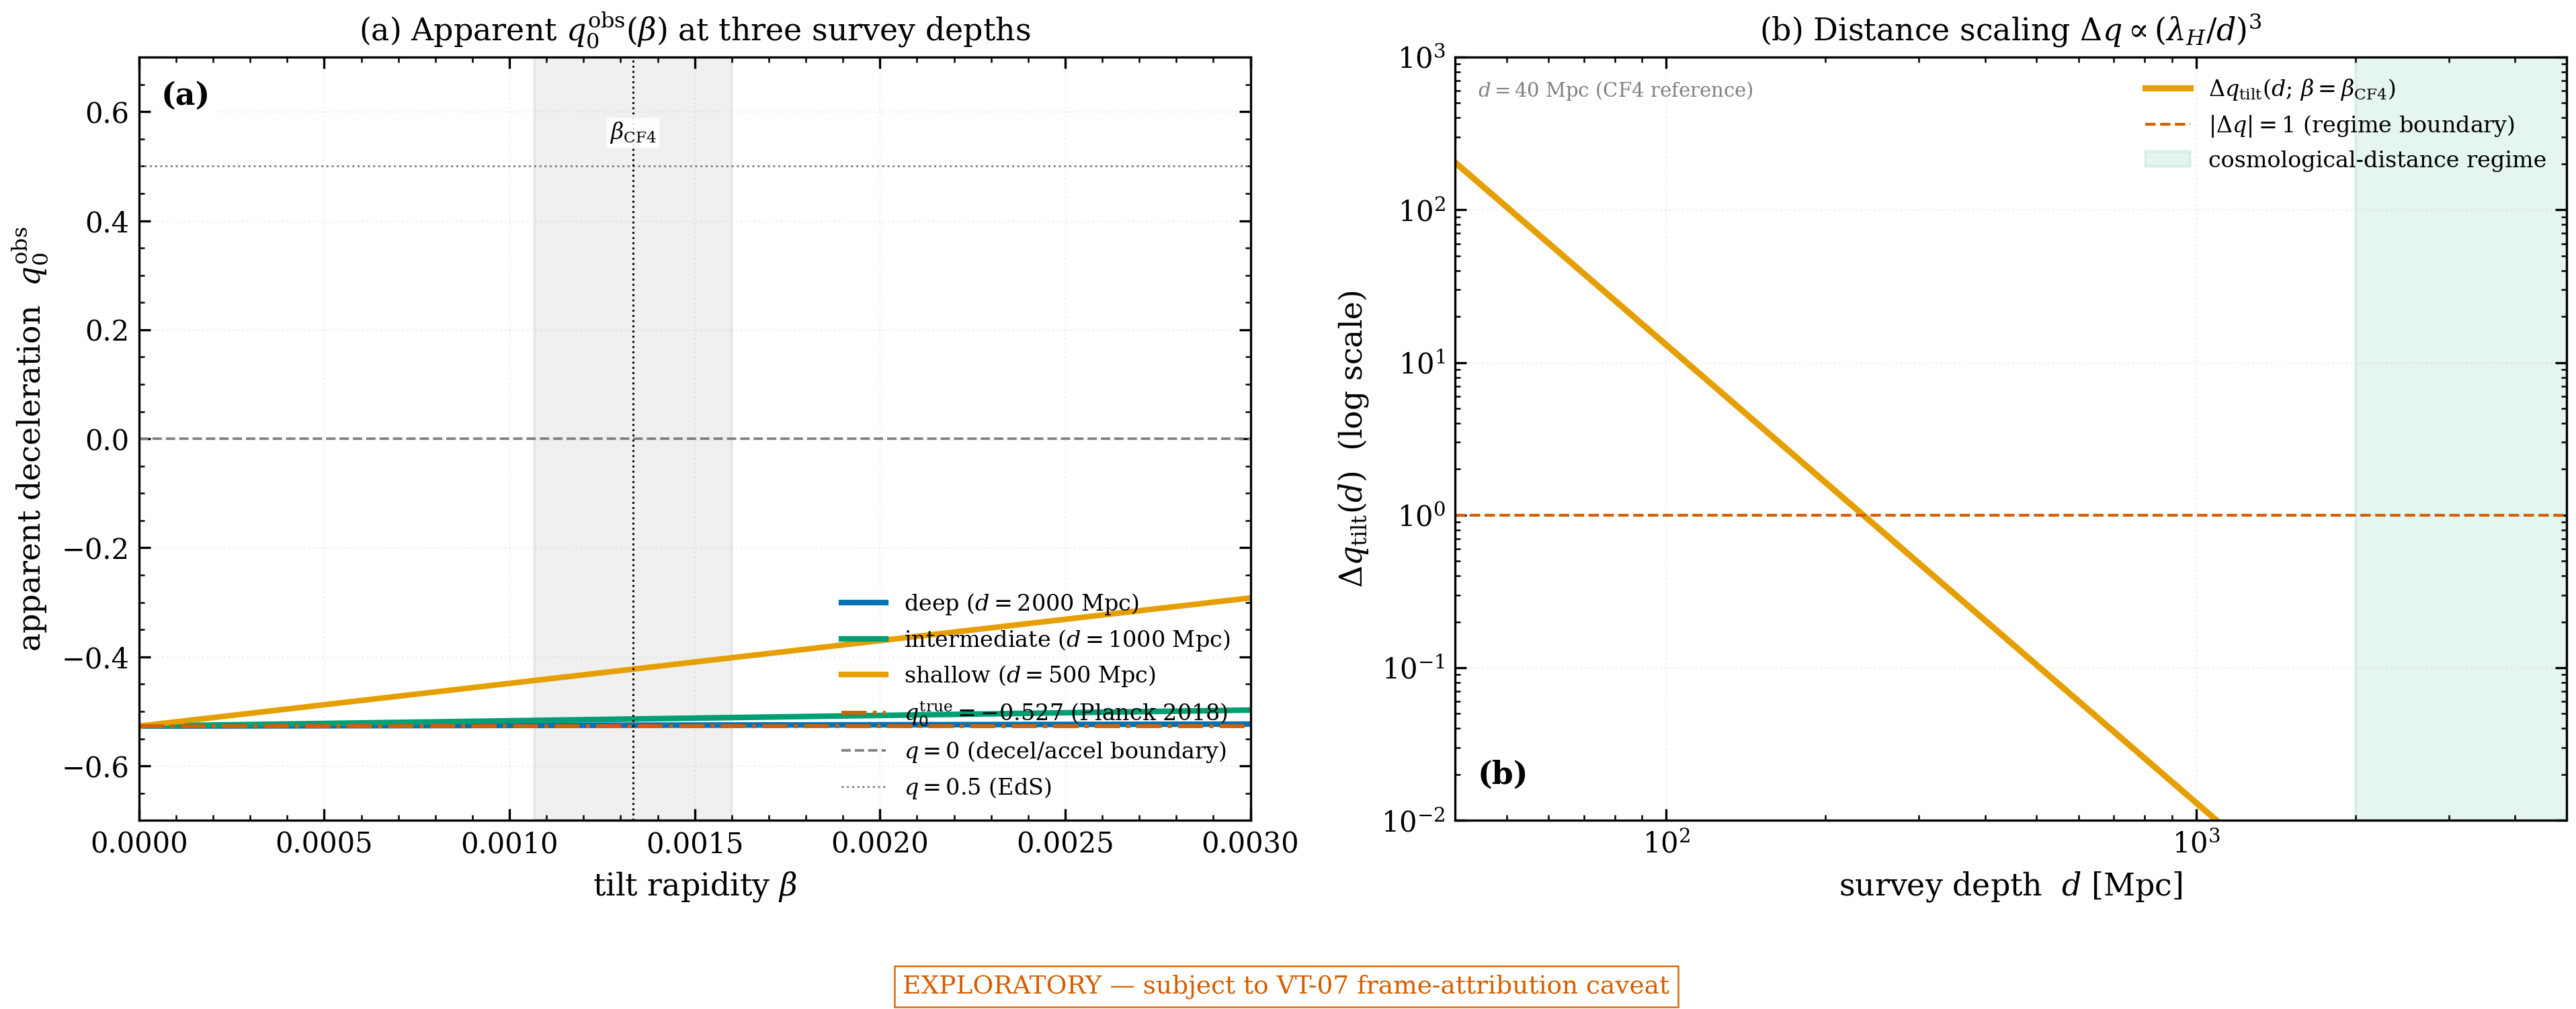
\includegraphics[width=0.82\textwidth,height=0.58\textheight,keepaspectratio]{conditioned_legacy/quarantined-legacy-root-sources__fig_q_decomposition}
\captionof{figure}{Conditioned legacy diagnostic: q decomposition. Condition: legacy manuscript-generator assumptions. See sidecar manifest for provenance and caveats; appendix-only, not native-transfer or family-ID evidence.}
\label{fig:conditioned-legacy-quarantined-legacy-root-sources-fig-q-decomposition}
\end{center}

\clearpage
\begin{center}
\centering
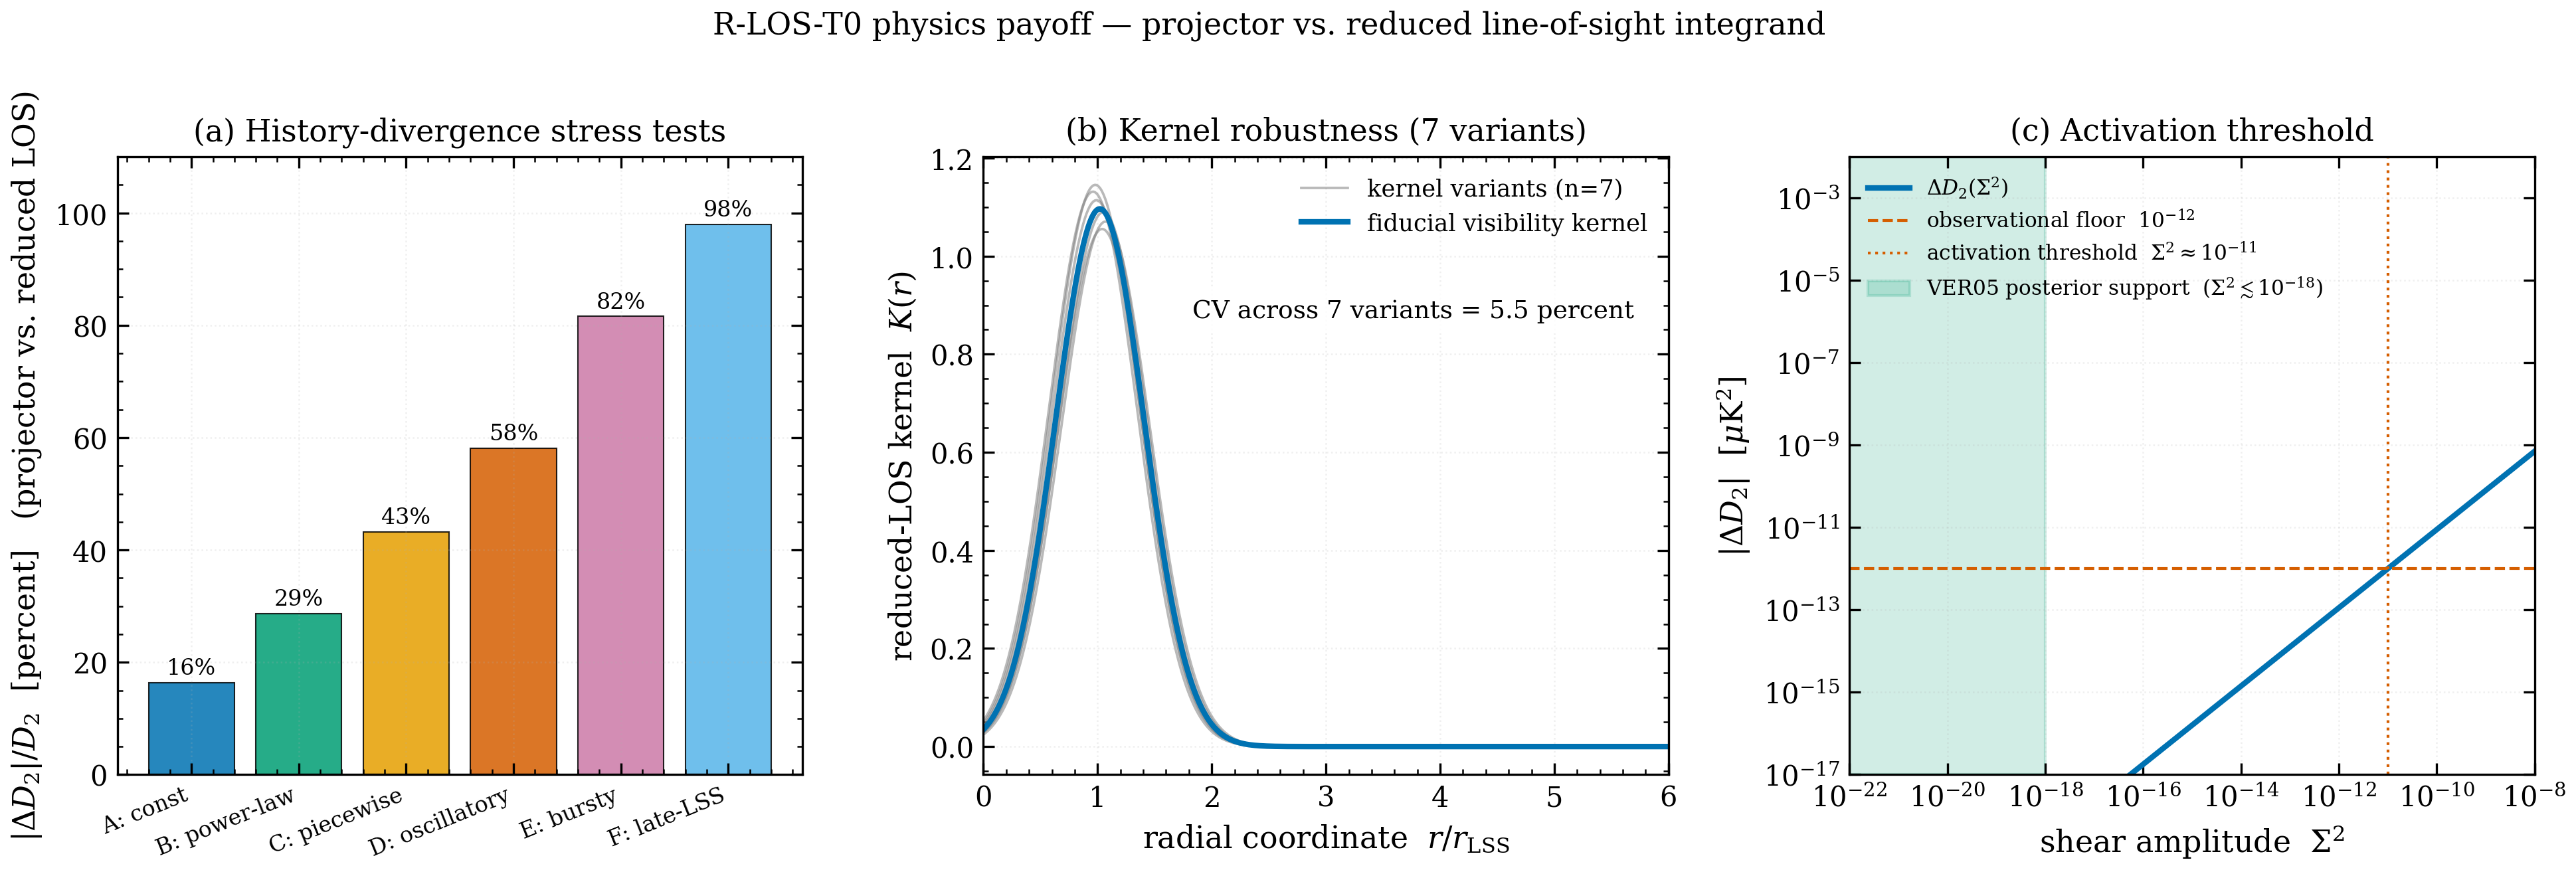
\includegraphics[width=0.82\textwidth,height=0.58\textheight,keepaspectratio]{conditioned_legacy/quarantined-legacy-root-sources__fig_reduced_los_physics_payoff}
\captionof{figure}{Conditioned legacy diagnostic: reduced los physics payoff. Condition: legacy manuscript-generator assumptions. See sidecar manifest for provenance and caveats; appendix-only, not native-transfer or family-ID evidence.}
\label{fig:conditioned-legacy-quarantined-legacy-root-sources-fig-reduced-los-physics-payoff}
\end{center}

\clearpage
\begin{center}
\centering
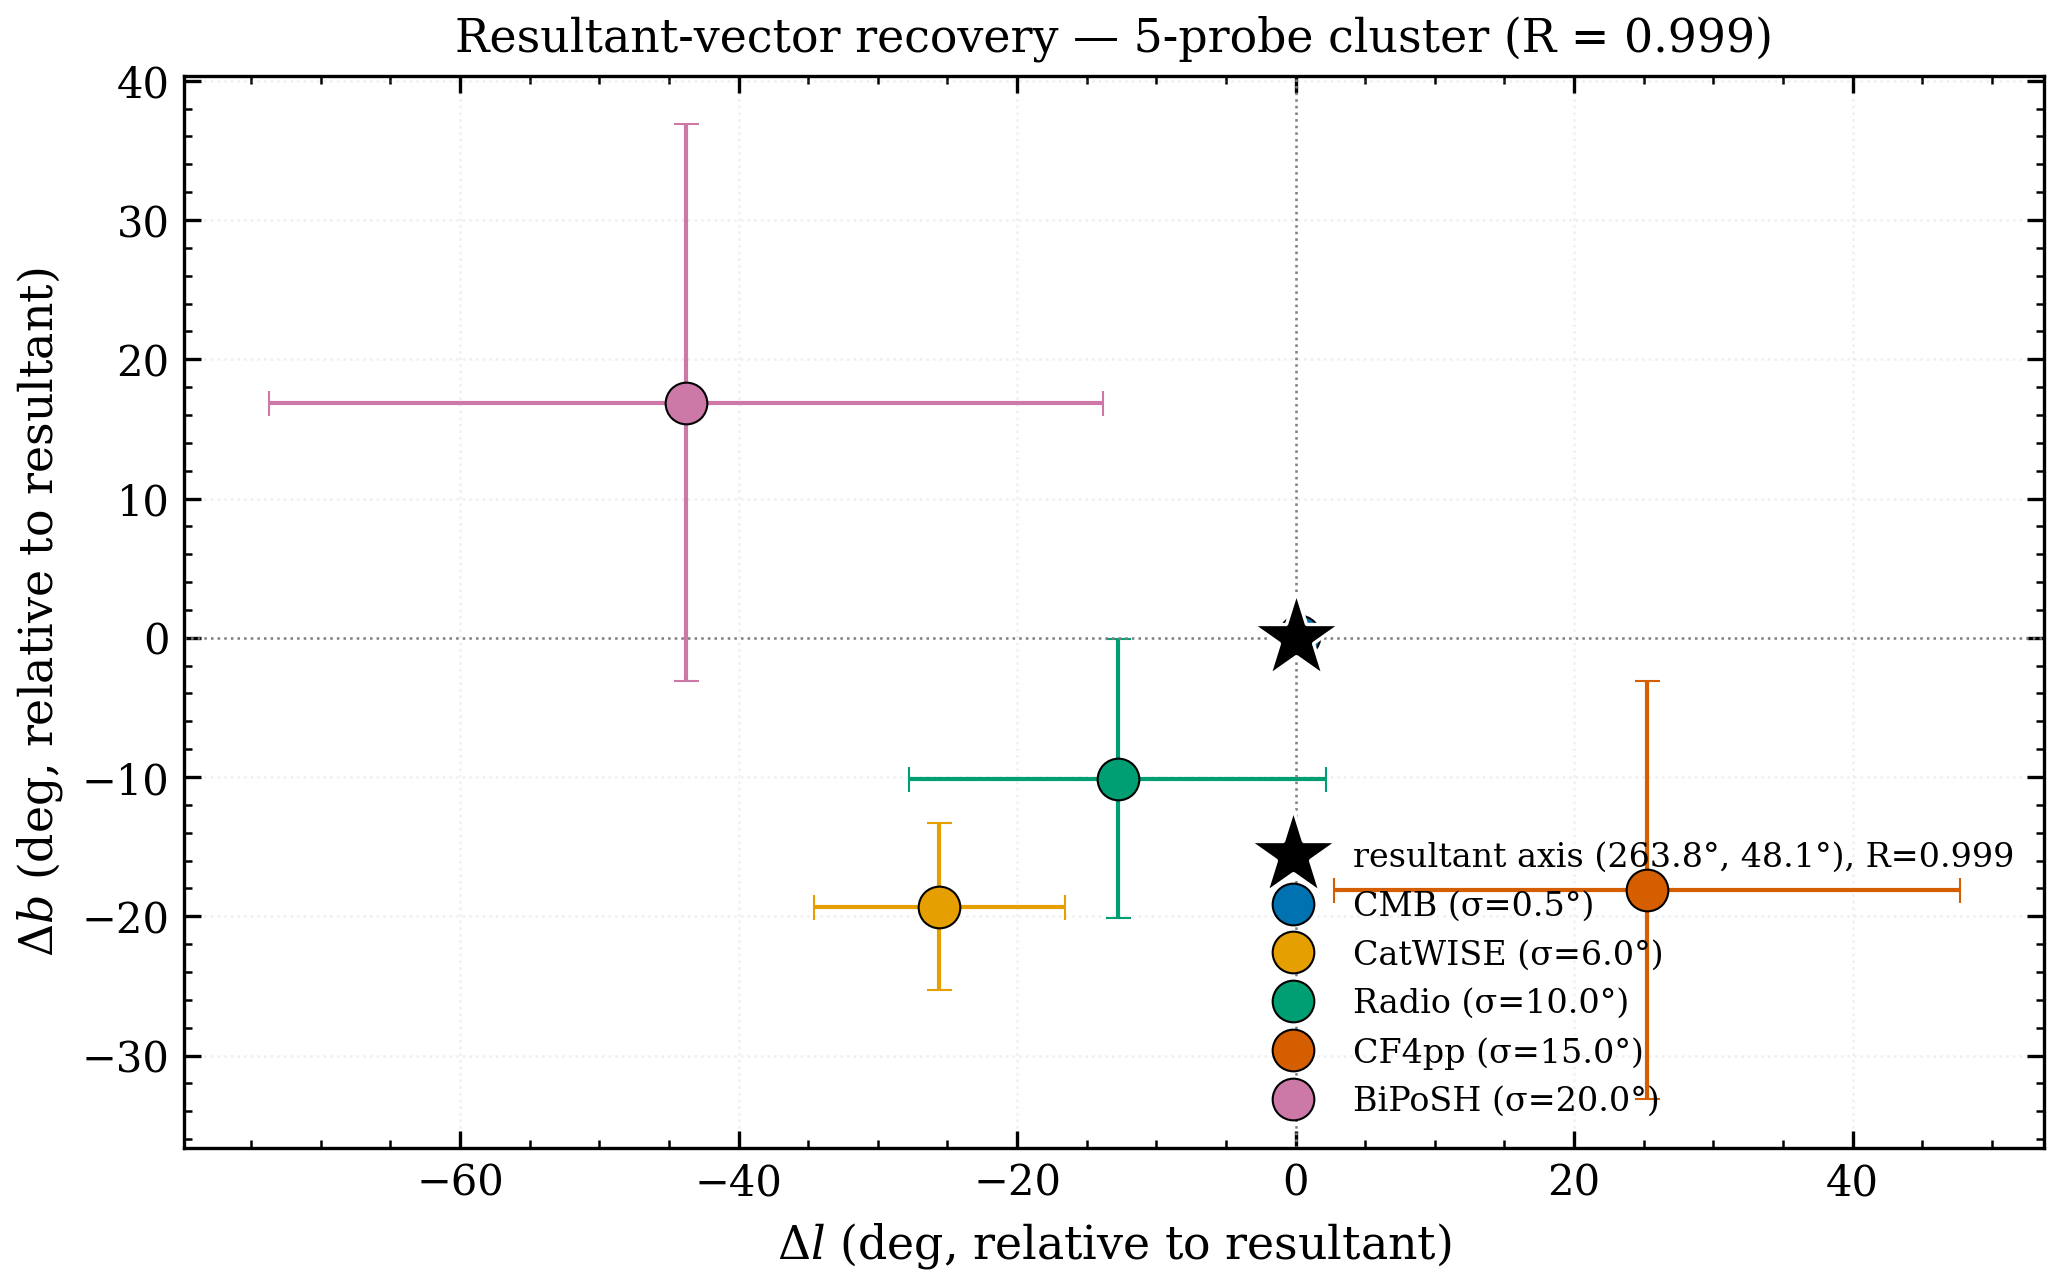
\includegraphics[width=0.82\textwidth,height=0.58\textheight,keepaspectratio]{conditioned_legacy/quarantined-legacy-root-sources__fig_resultant_vector_5probes}
\captionof{figure}{Conditioned legacy diagnostic: resultant vector 5probes. Condition: legacy manuscript-generator assumptions. See sidecar manifest for provenance and caveats; appendix-only, not native-transfer or family-ID evidence.}
\label{fig:conditioned-legacy-quarantined-legacy-root-sources-fig-resultant-vector-5probes}
\end{center}

\clearpage
\begin{center}
\centering
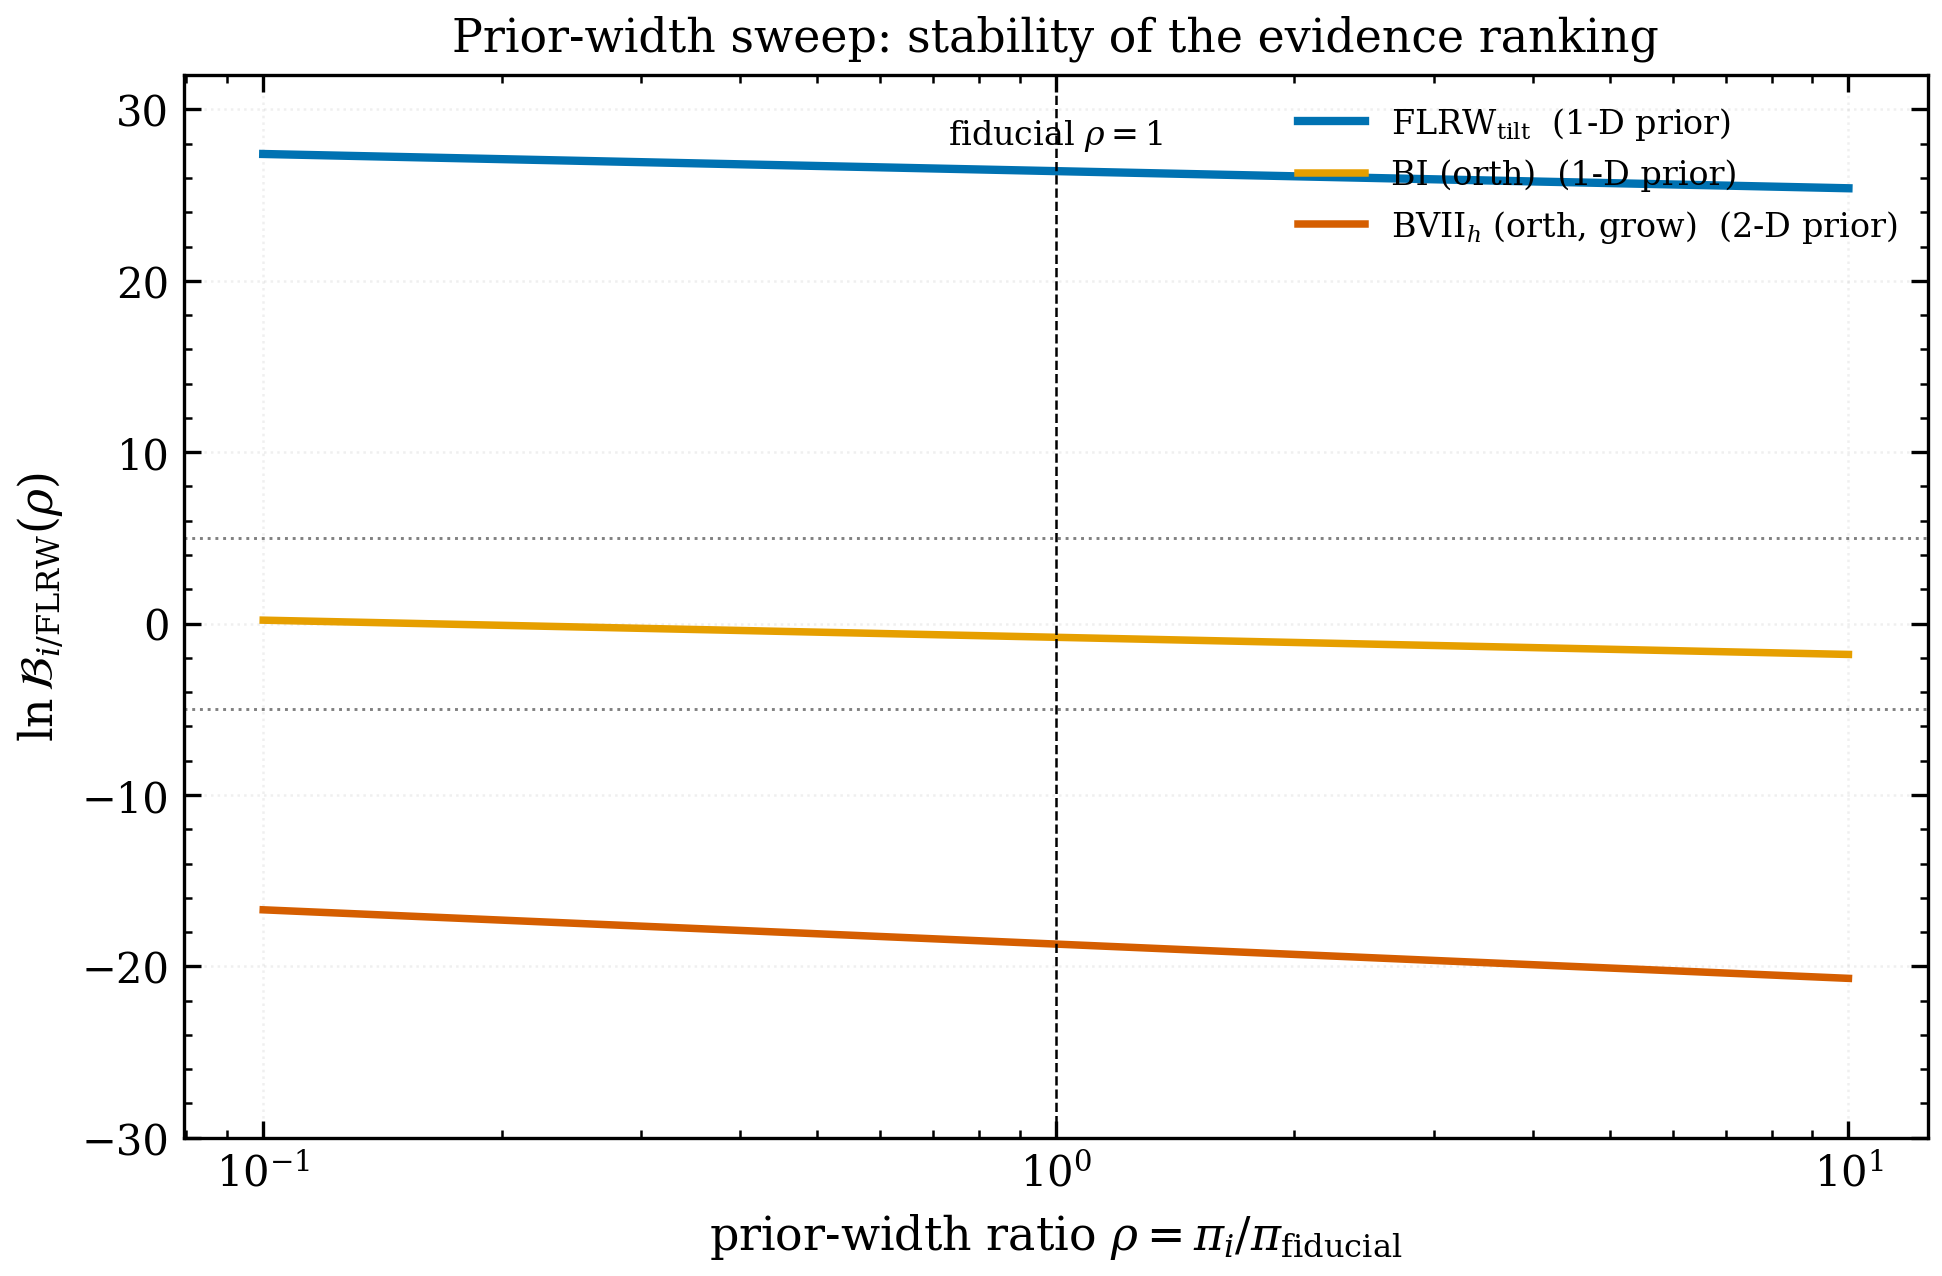
\includegraphics[width=0.82\textwidth,height=0.58\textheight,keepaspectratio]{conditioned_legacy/quarantined-legacy-root-sources__fig_rho_sweep}
\captionof{figure}{Conditioned legacy diagnostic: rho sweep. Condition: legacy manuscript-generator assumptions. See sidecar manifest for provenance and caveats; appendix-only, not native-transfer or family-ID evidence.}
\label{fig:conditioned-legacy-quarantined-legacy-root-sources-fig-rho-sweep}
\end{center}

\clearpage
\begin{center}
\centering
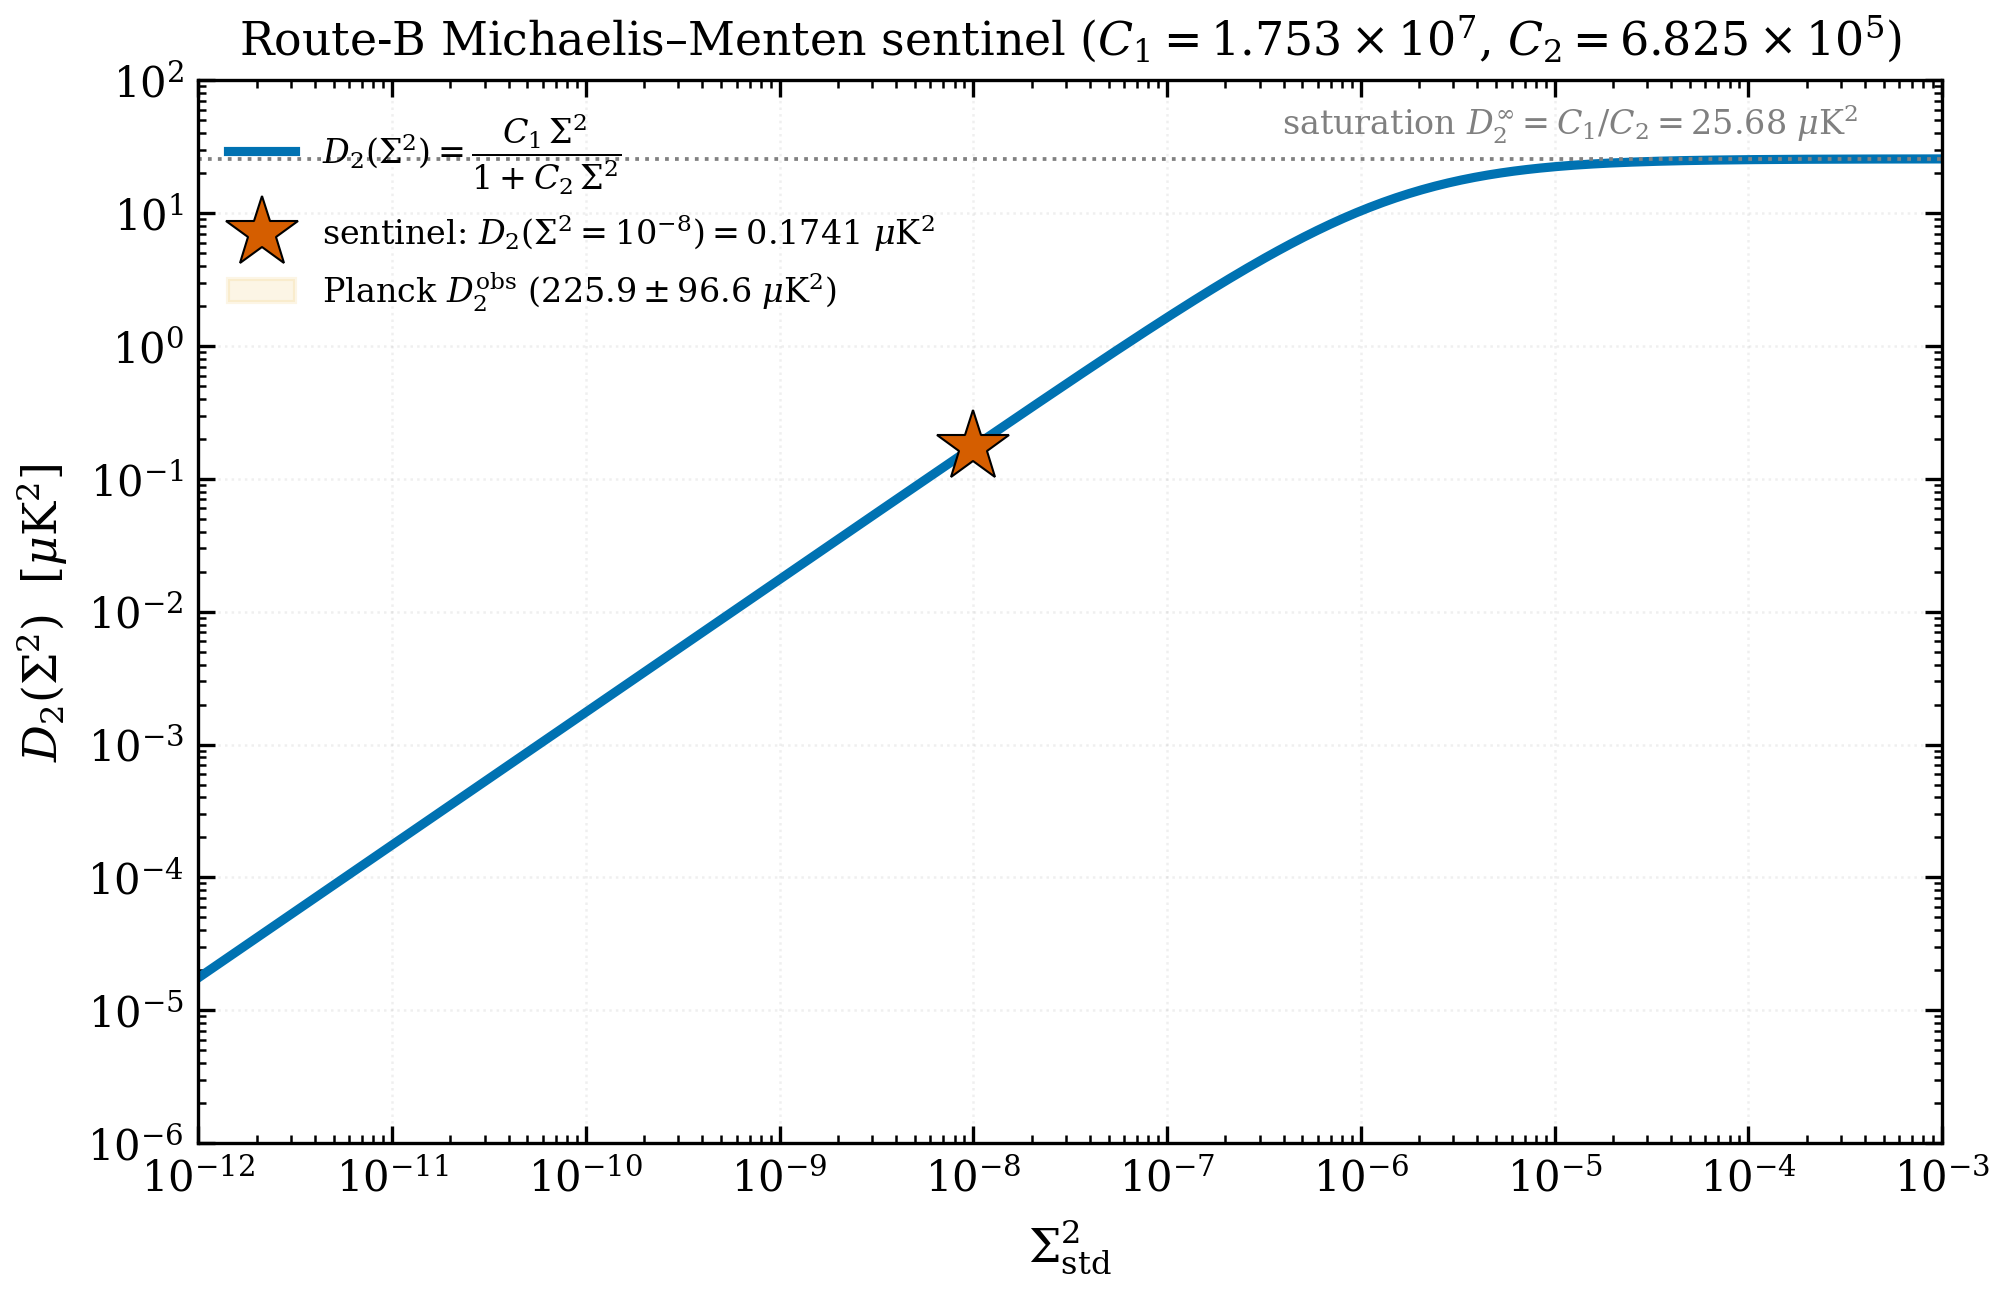
\includegraphics[width=0.82\textwidth,height=0.58\textheight,keepaspectratio]{conditioned_legacy/quarantined-legacy-root-sources__fig_route_b_mm_curve}
\captionof{figure}{Conditioned legacy diagnostic: route b mm curve. Condition: legacy manuscript-generator assumptions. See sidecar manifest for provenance and caveats; appendix-only, not native-transfer or family-ID evidence.}
\label{fig:conditioned-legacy-quarantined-legacy-root-sources-fig-route-b-mm-curve}
\end{center}

\clearpage
\begin{center}
\centering
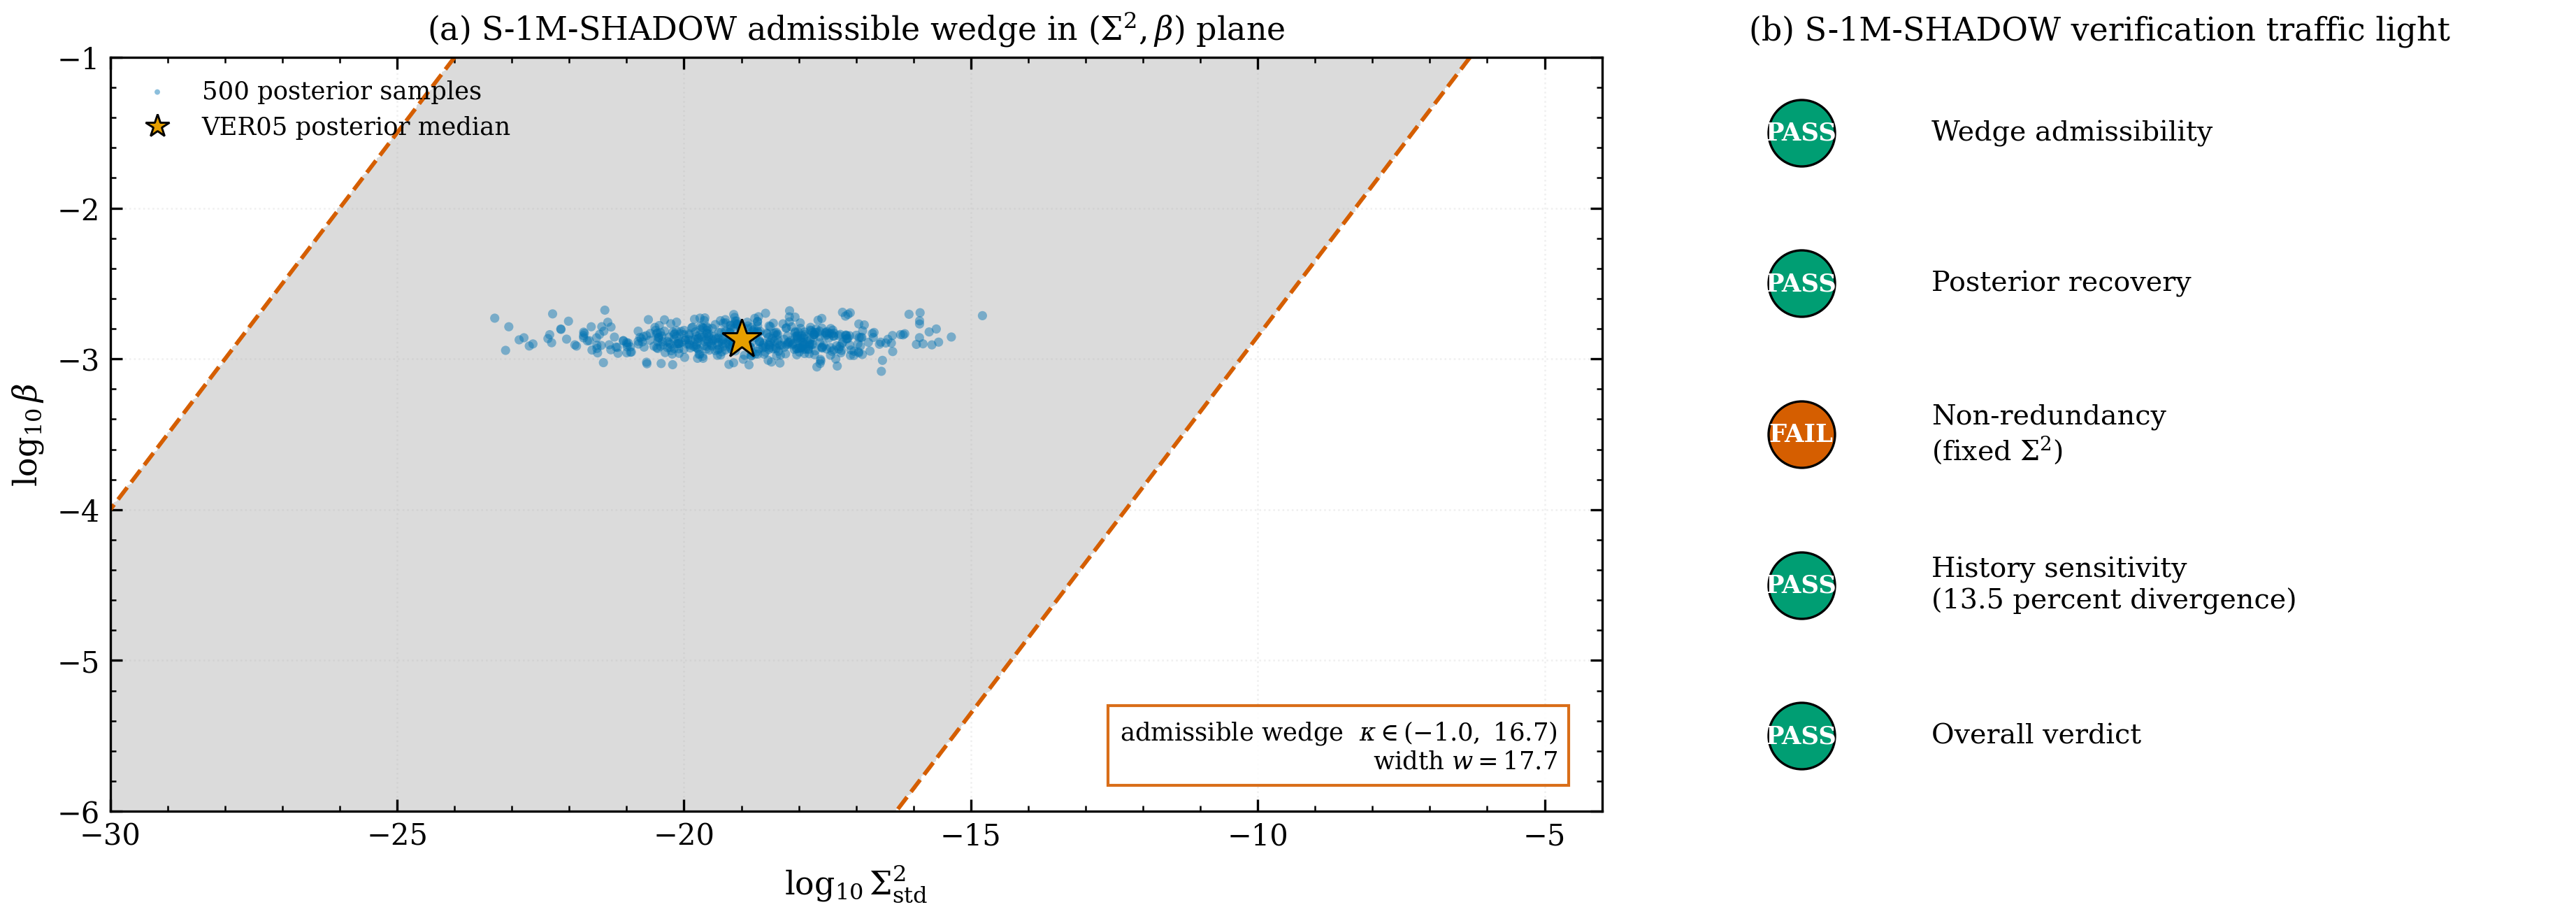
\includegraphics[width=0.82\textwidth,height=0.58\textheight,keepaspectratio]{conditioned_legacy/quarantined-legacy-root-sources__fig_s1m_shadow}
\captionof{figure}{Conditioned legacy diagnostic: s1m shadow. Condition: legacy manuscript-generator assumptions. See sidecar manifest for provenance and caveats; appendix-only, not native-transfer or family-ID evidence.}
\label{fig:conditioned-legacy-quarantined-legacy-root-sources-fig-s1m-shadow}
\end{center}

\clearpage
\begin{center}
\centering
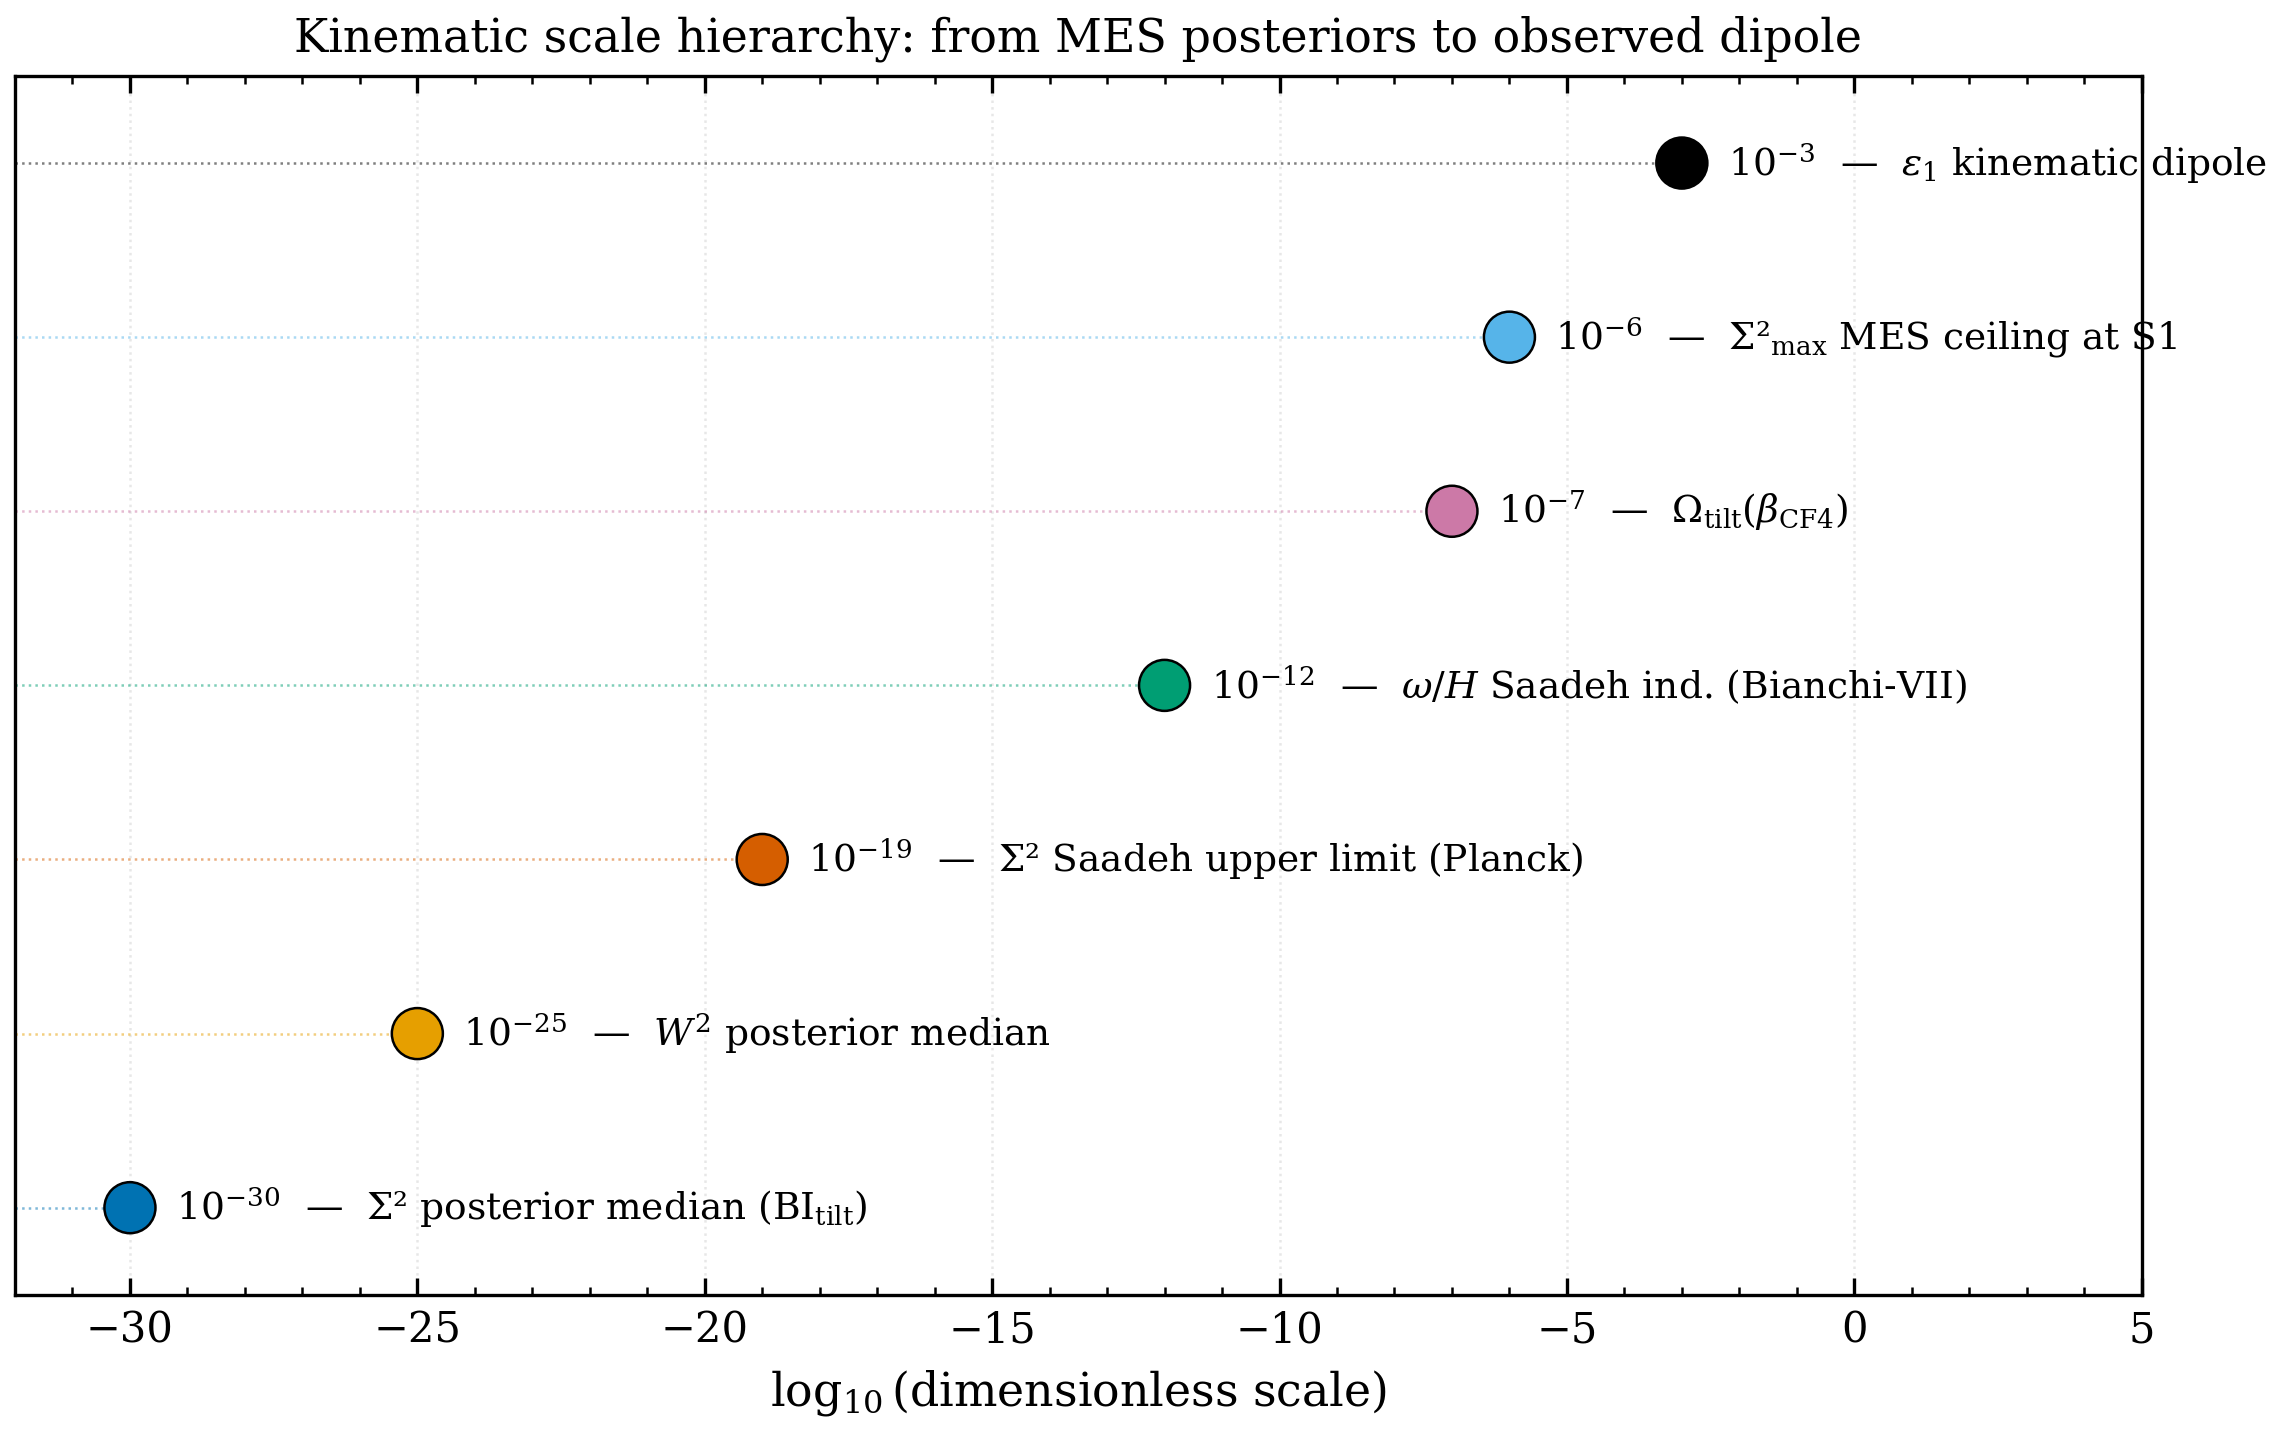
\includegraphics[width=0.82\textwidth,height=0.58\textheight,keepaspectratio]{conditioned_legacy/quarantined-legacy-root-sources__fig_scale_hierarchy}
\captionof{figure}{Conditioned legacy diagnostic: scale hierarchy. Condition: legacy manuscript-generator assumptions. See sidecar manifest for provenance and caveats; appendix-only, not native-transfer or family-ID evidence.}
\label{fig:conditioned-legacy-quarantined-legacy-root-sources-fig-scale-hierarchy}
\end{center}

\clearpage
\begin{center}
\centering
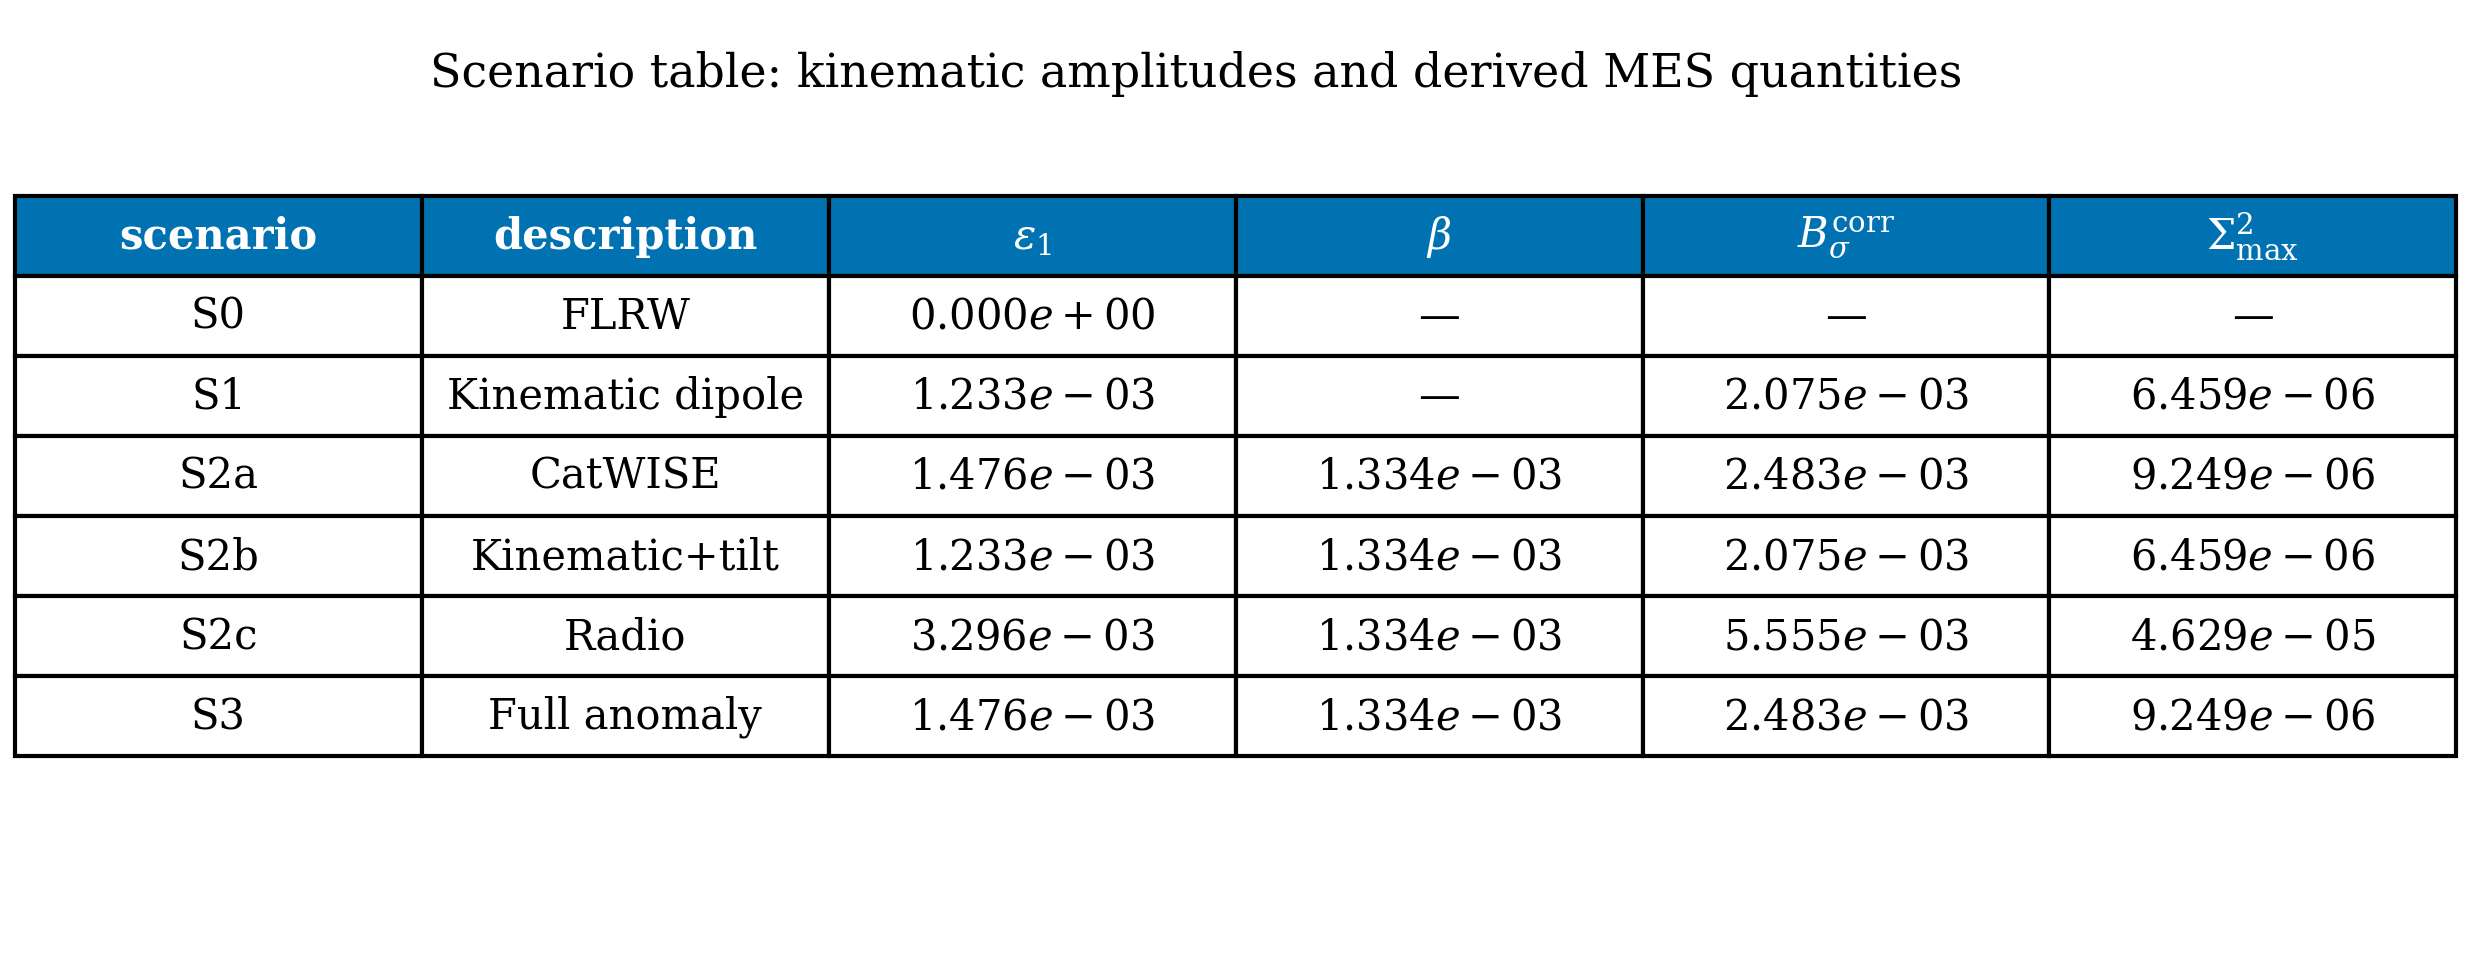
\includegraphics[width=0.82\textwidth,height=0.58\textheight,keepaspectratio]{conditioned_legacy/quarantined-legacy-root-sources__fig_scenarios_comprehensive}
\captionof{figure}{Conditioned legacy diagnostic: scenarios comprehensive. Condition: legacy manuscript-generator assumptions. See sidecar manifest for provenance and caveats; appendix-only, not native-transfer or family-ID evidence.}
\label{fig:conditioned-legacy-quarantined-legacy-root-sources-fig-scenarios-comprehensive}
\end{center}

\clearpage
\begin{center}
\centering
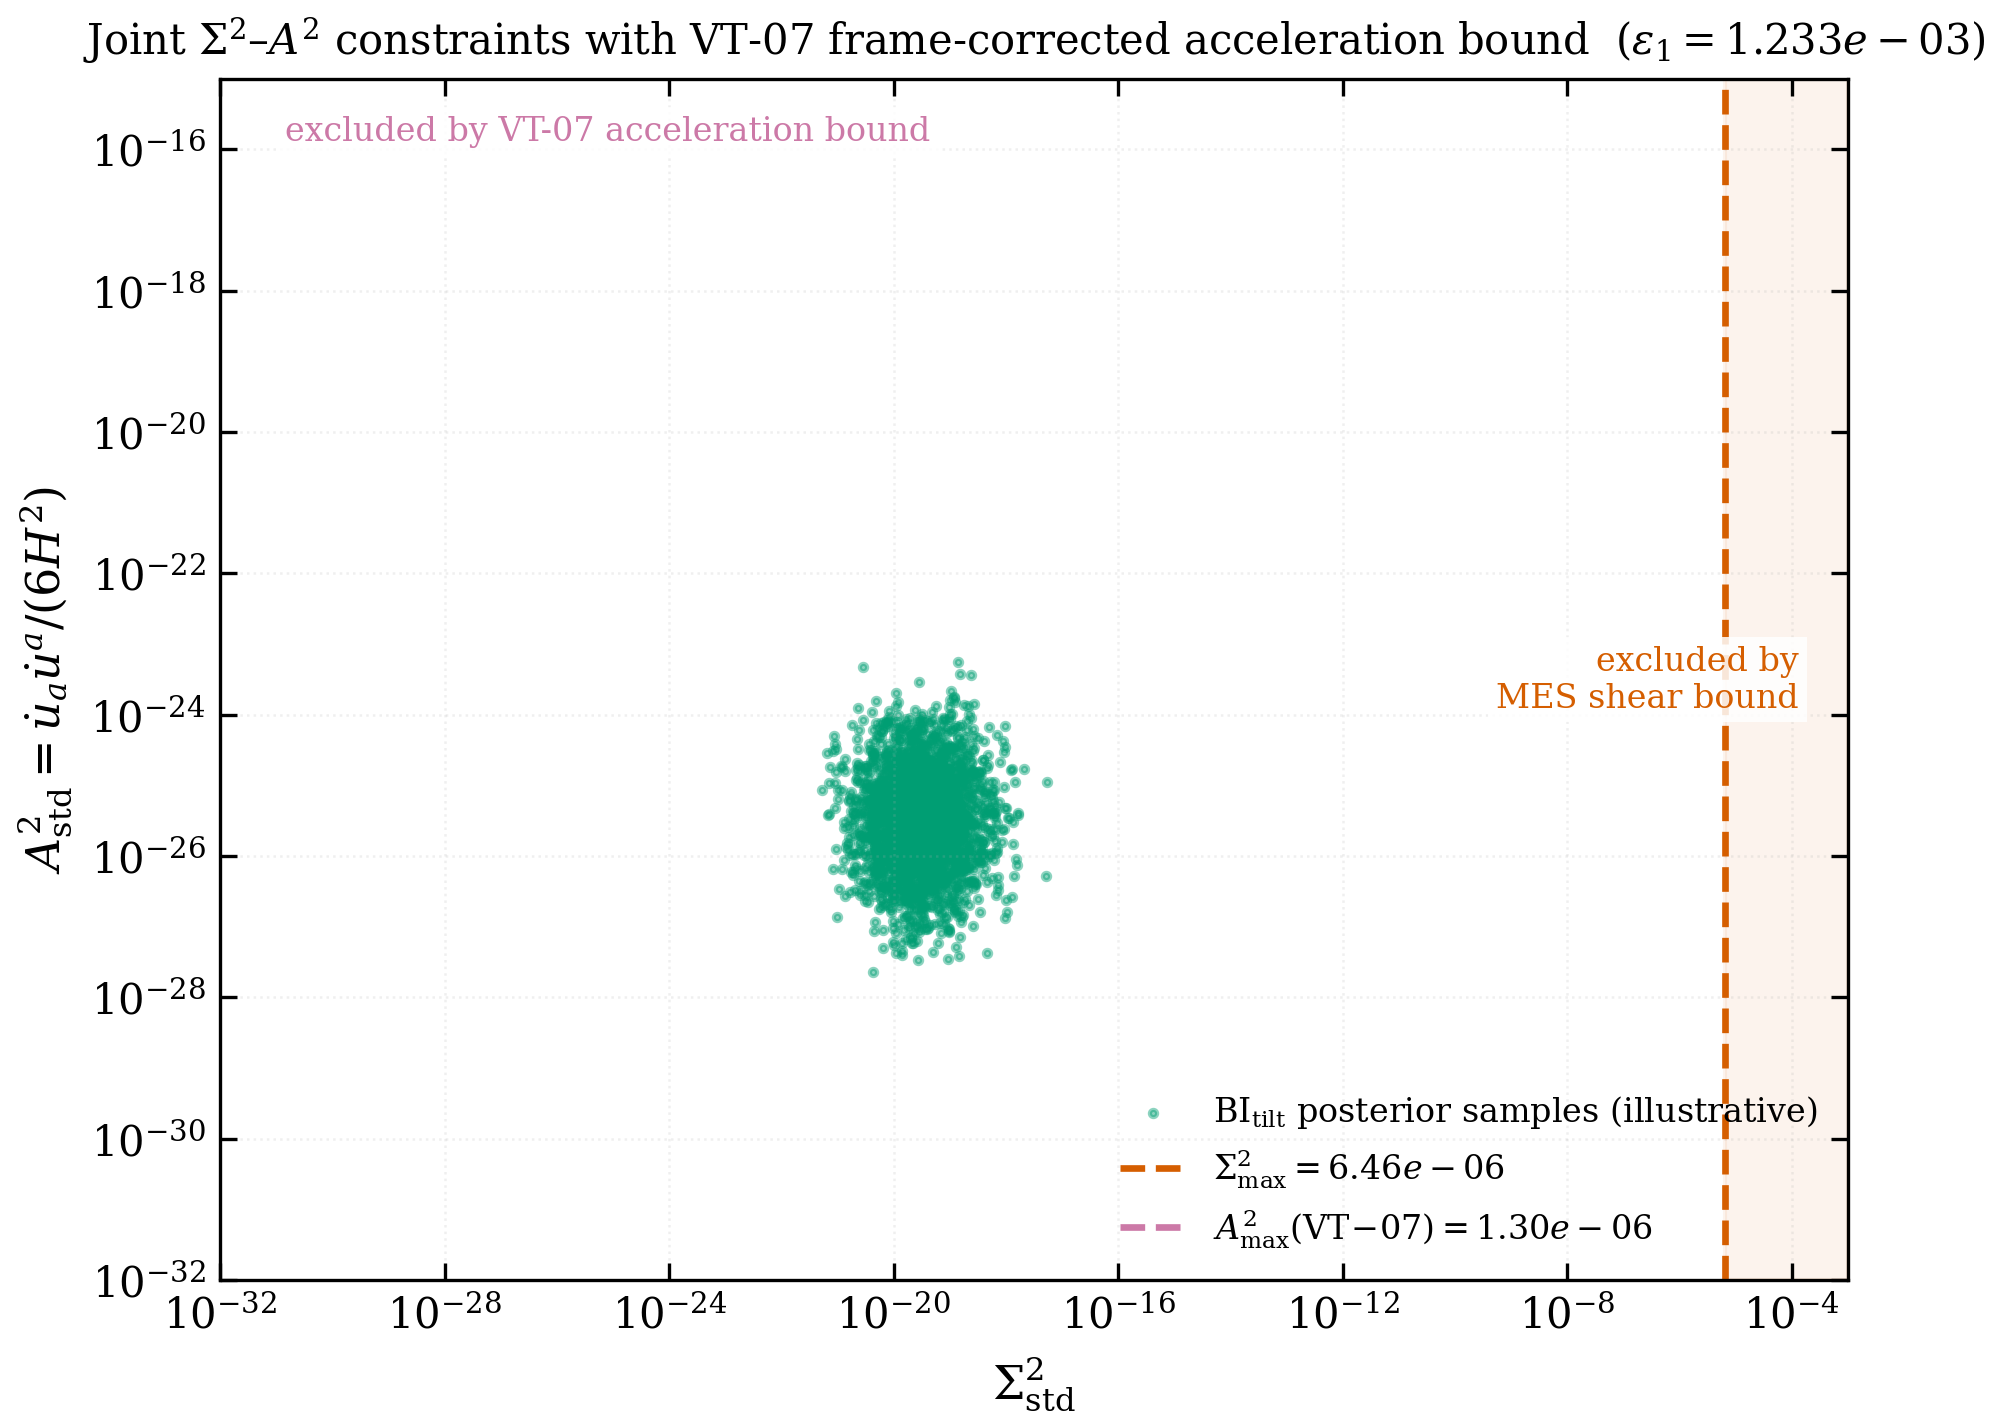
\includegraphics[width=0.82\textwidth,height=0.58\textheight,keepaspectratio]{conditioned_legacy/quarantined-legacy-root-sources__fig_sigma_accel_contour}
\captionof{figure}{Conditioned legacy diagnostic: sigma accel contour. Condition: legacy manuscript-generator assumptions. See sidecar manifest for provenance and caveats; appendix-only, not native-transfer or family-ID evidence.}
\label{fig:conditioned-legacy-quarantined-legacy-root-sources-fig-sigma-accel-contour}
\end{center}

\clearpage
\begin{center}
\centering
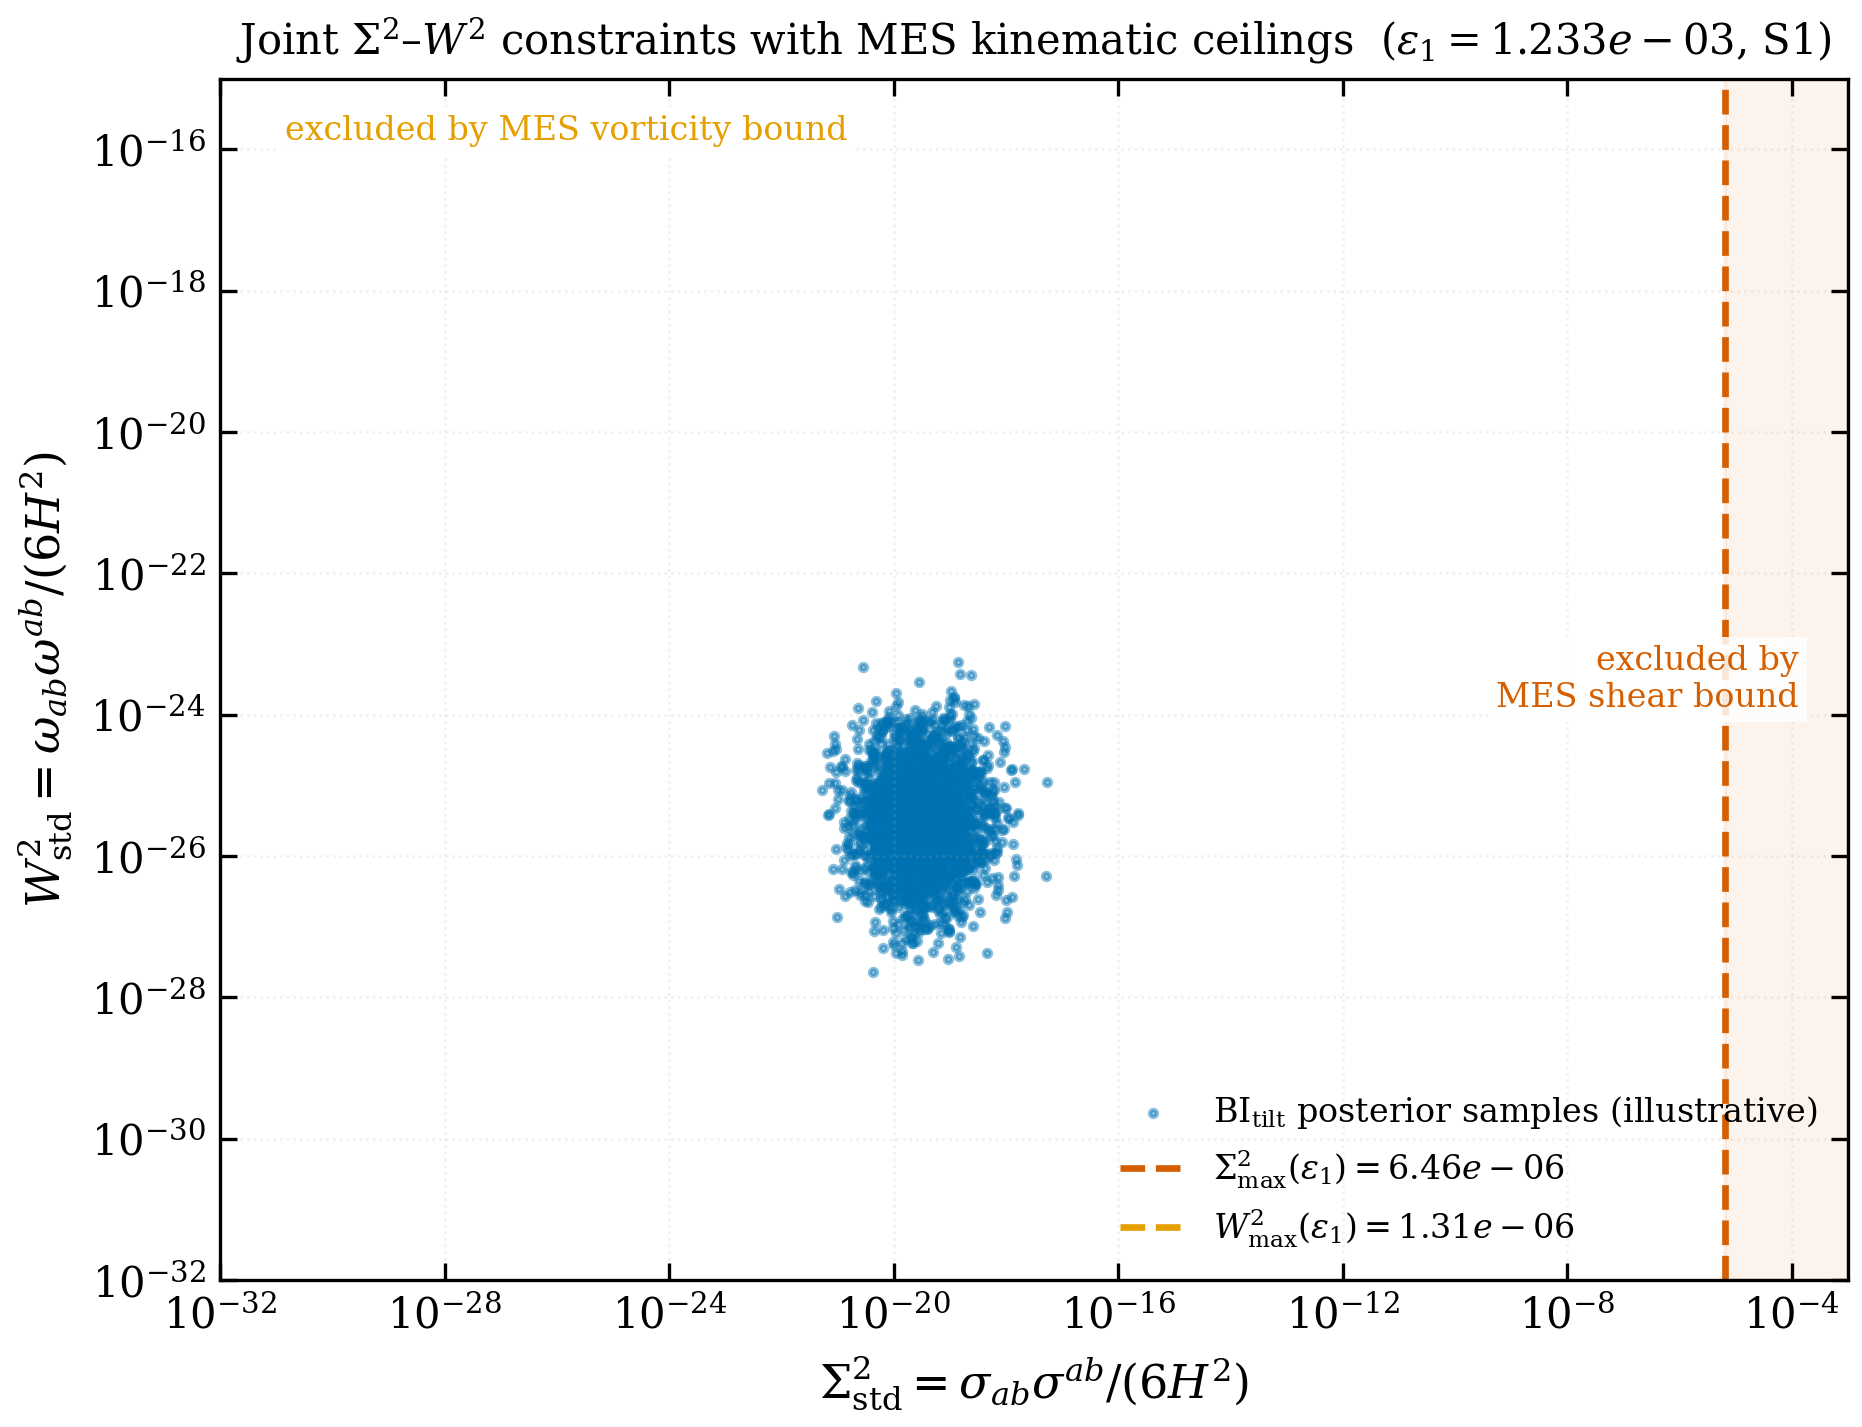
\includegraphics[width=0.82\textwidth,height=0.58\textheight,keepaspectratio]{conditioned_legacy/quarantined-legacy-root-sources__fig_sigma_omega_contour}
\captionof{figure}{Conditioned legacy diagnostic: sigma omega contour. Condition: legacy manuscript-generator assumptions. See sidecar manifest for provenance and caveats; appendix-only, not native-transfer or family-ID evidence.}
\label{fig:conditioned-legacy-quarantined-legacy-root-sources-fig-sigma-omega-contour}
\end{center}

\clearpage
\begin{center}
\centering
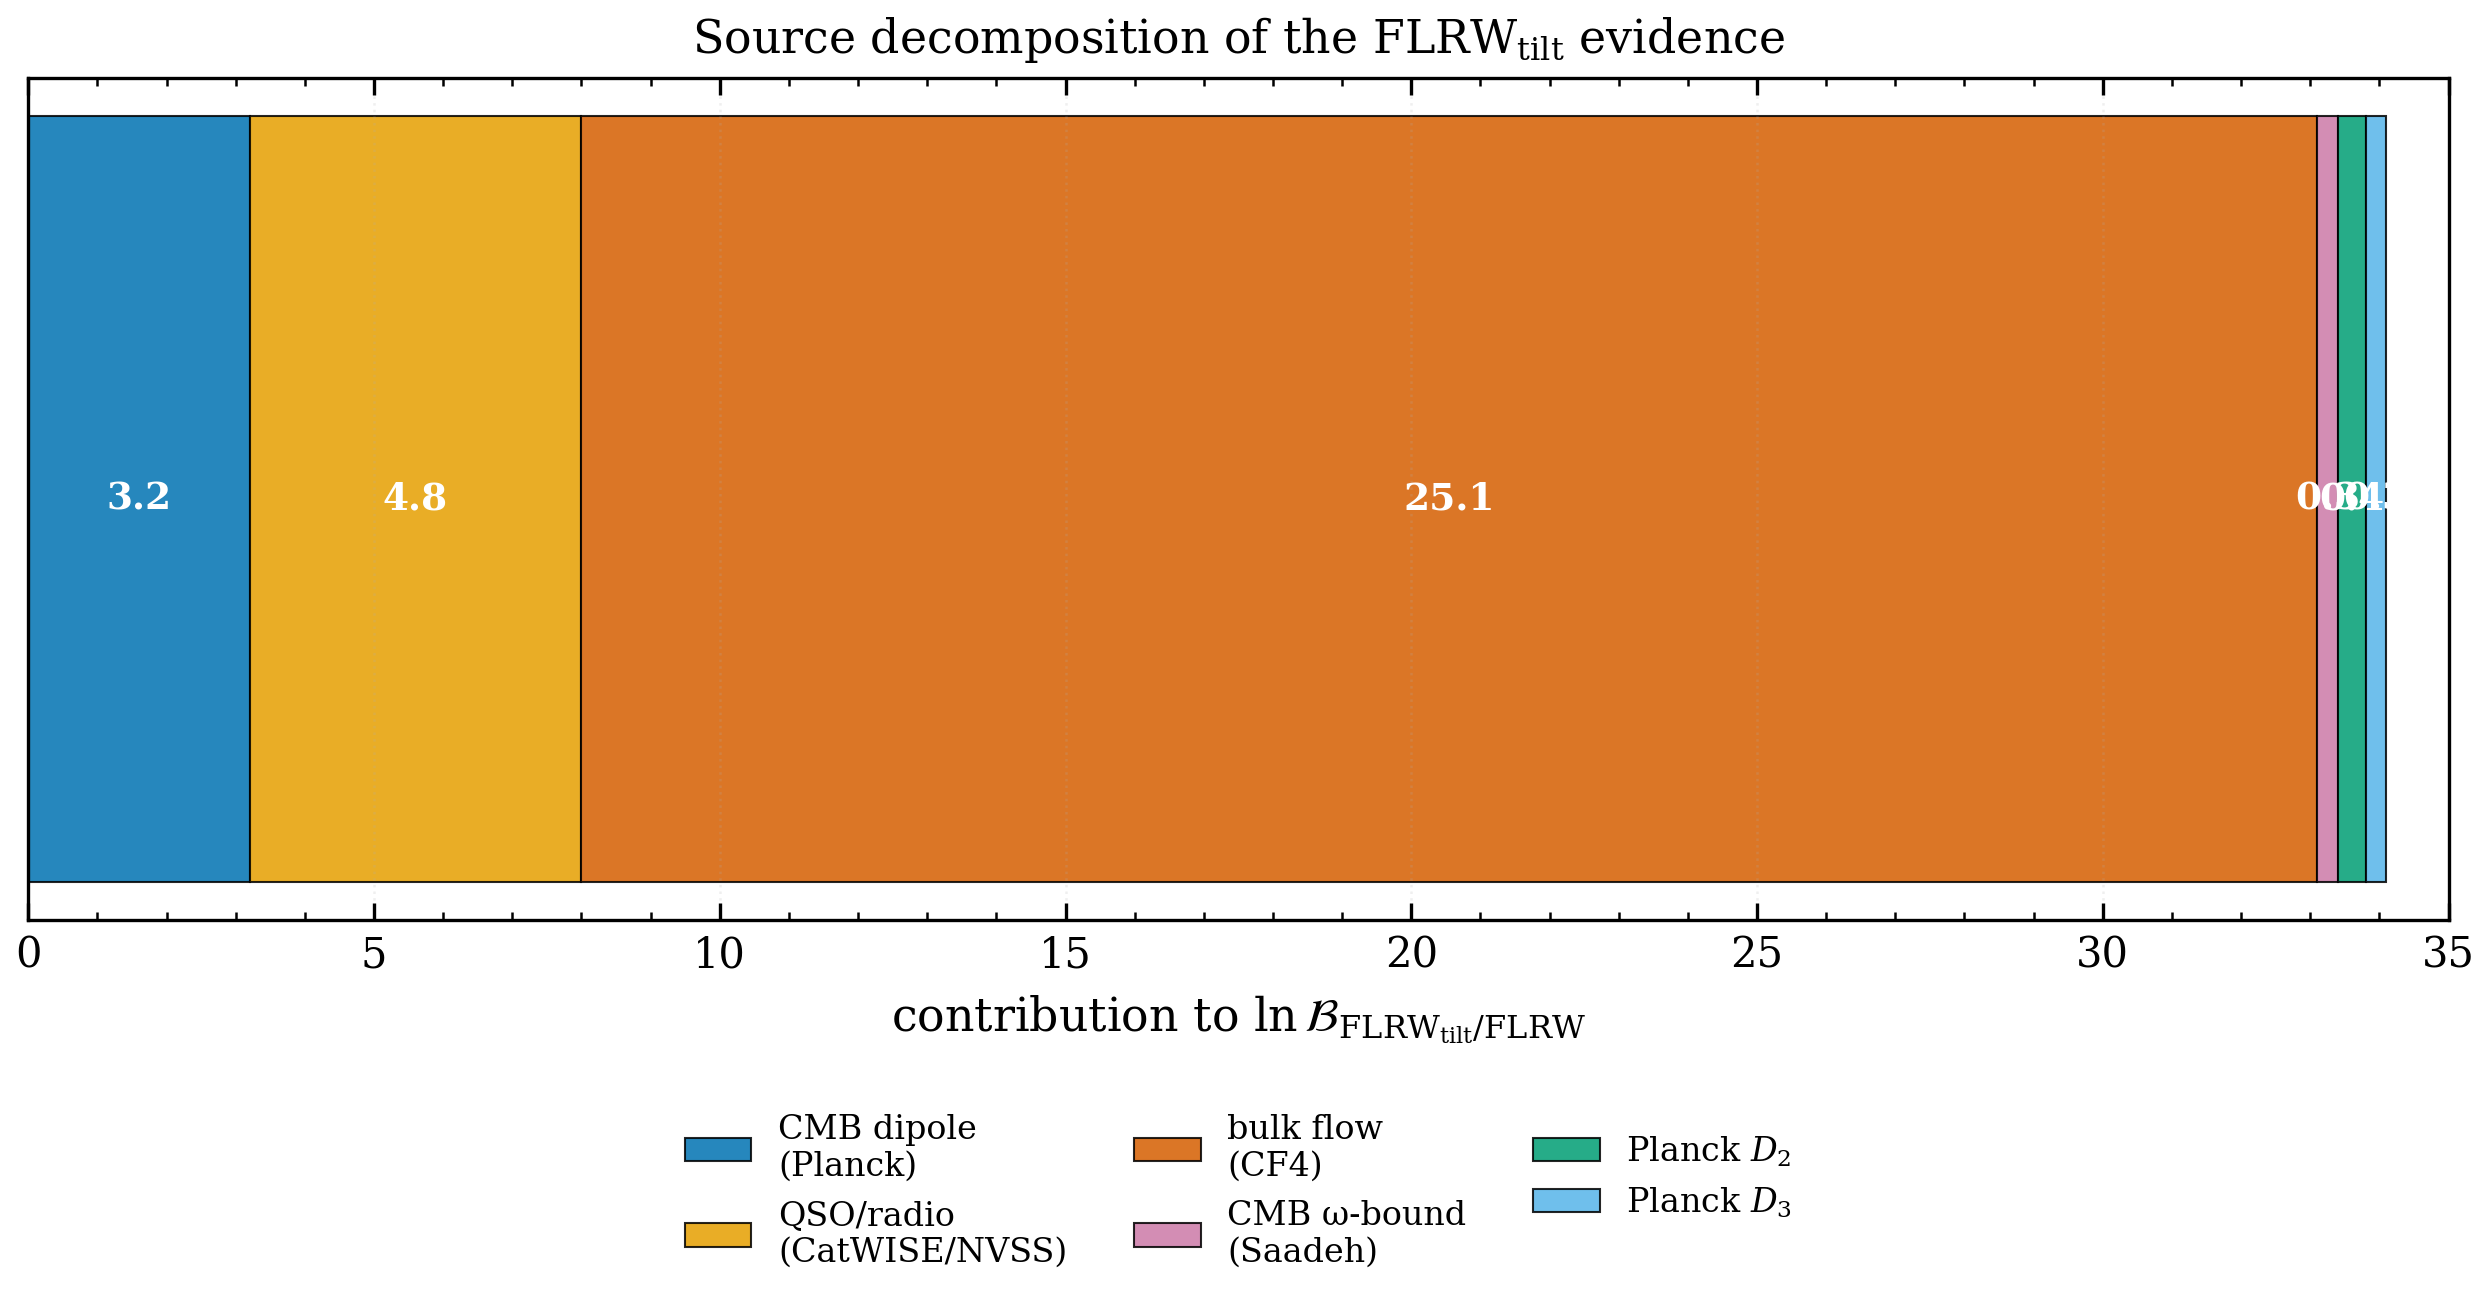
\includegraphics[width=0.82\textwidth,height=0.58\textheight,keepaspectratio]{conditioned_legacy/quarantined-legacy-root-sources__fig_source_decomposition}
\captionof{figure}{Conditioned legacy diagnostic: source decomposition. Condition: legacy manuscript-generator assumptions. See sidecar manifest for provenance and caveats; appendix-only, not native-transfer or family-ID evidence.}
\label{fig:conditioned-legacy-quarantined-legacy-root-sources-fig-source-decomposition}
\end{center}

\clearpage
\begin{center}
\centering
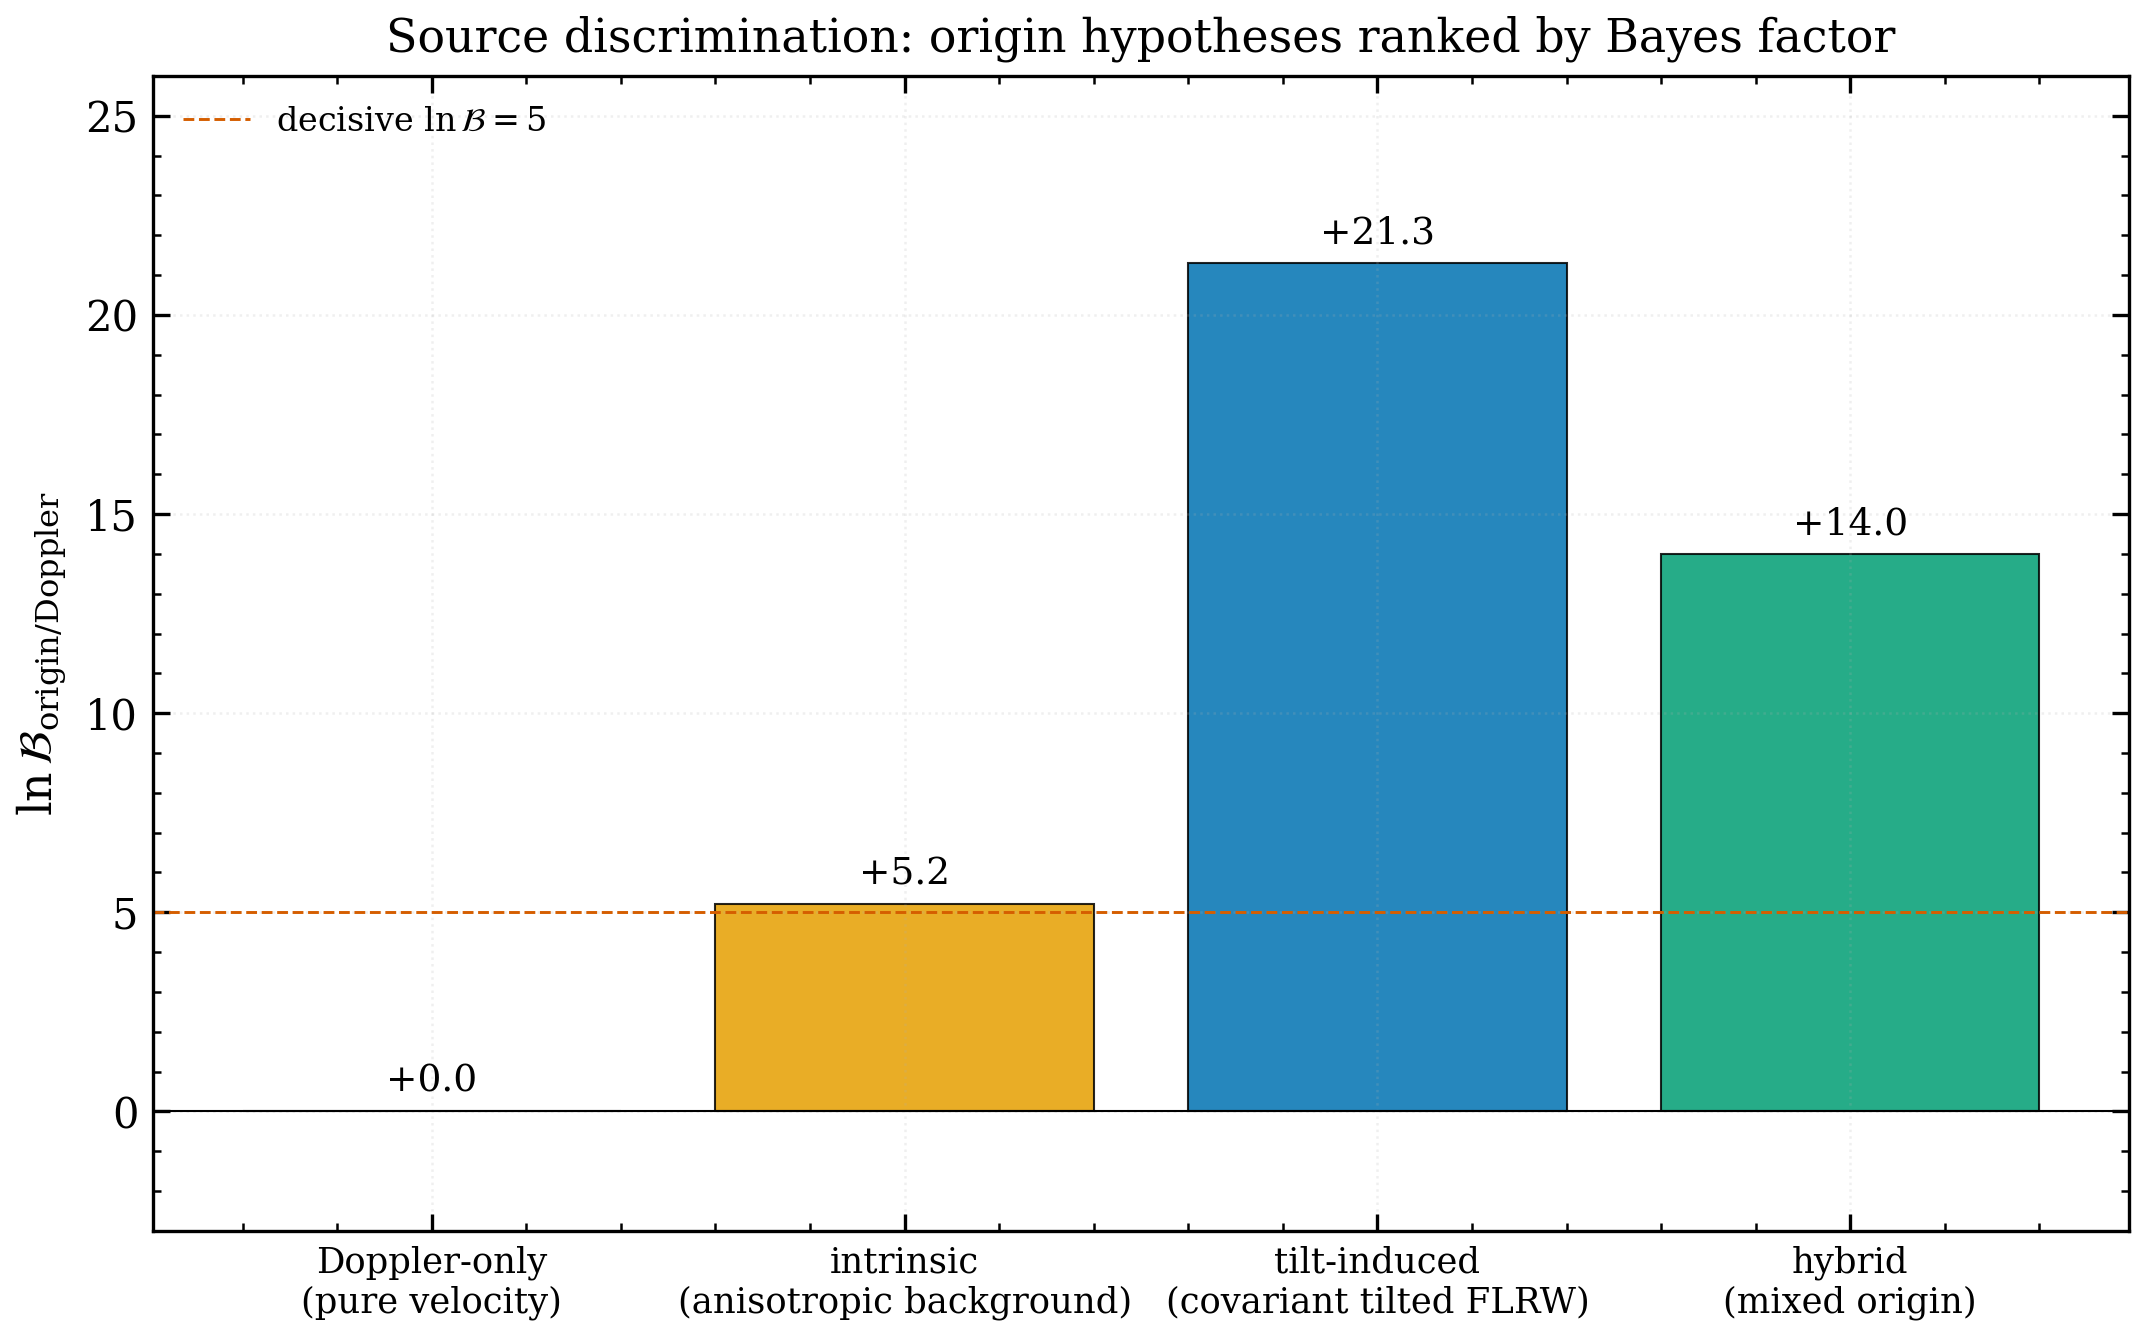
\includegraphics[width=0.82\textwidth,height=0.58\textheight,keepaspectratio]{conditioned_legacy/quarantined-legacy-root-sources__fig_source_discrimination}
\captionof{figure}{Conditioned legacy diagnostic: source discrimination. Condition: legacy manuscript-generator assumptions. See sidecar manifest for provenance and caveats; appendix-only, not native-transfer or family-ID evidence.}
\label{fig:conditioned-legacy-quarantined-legacy-root-sources-fig-source-discrimination}
\end{center}

\clearpage
\begin{center}
\centering
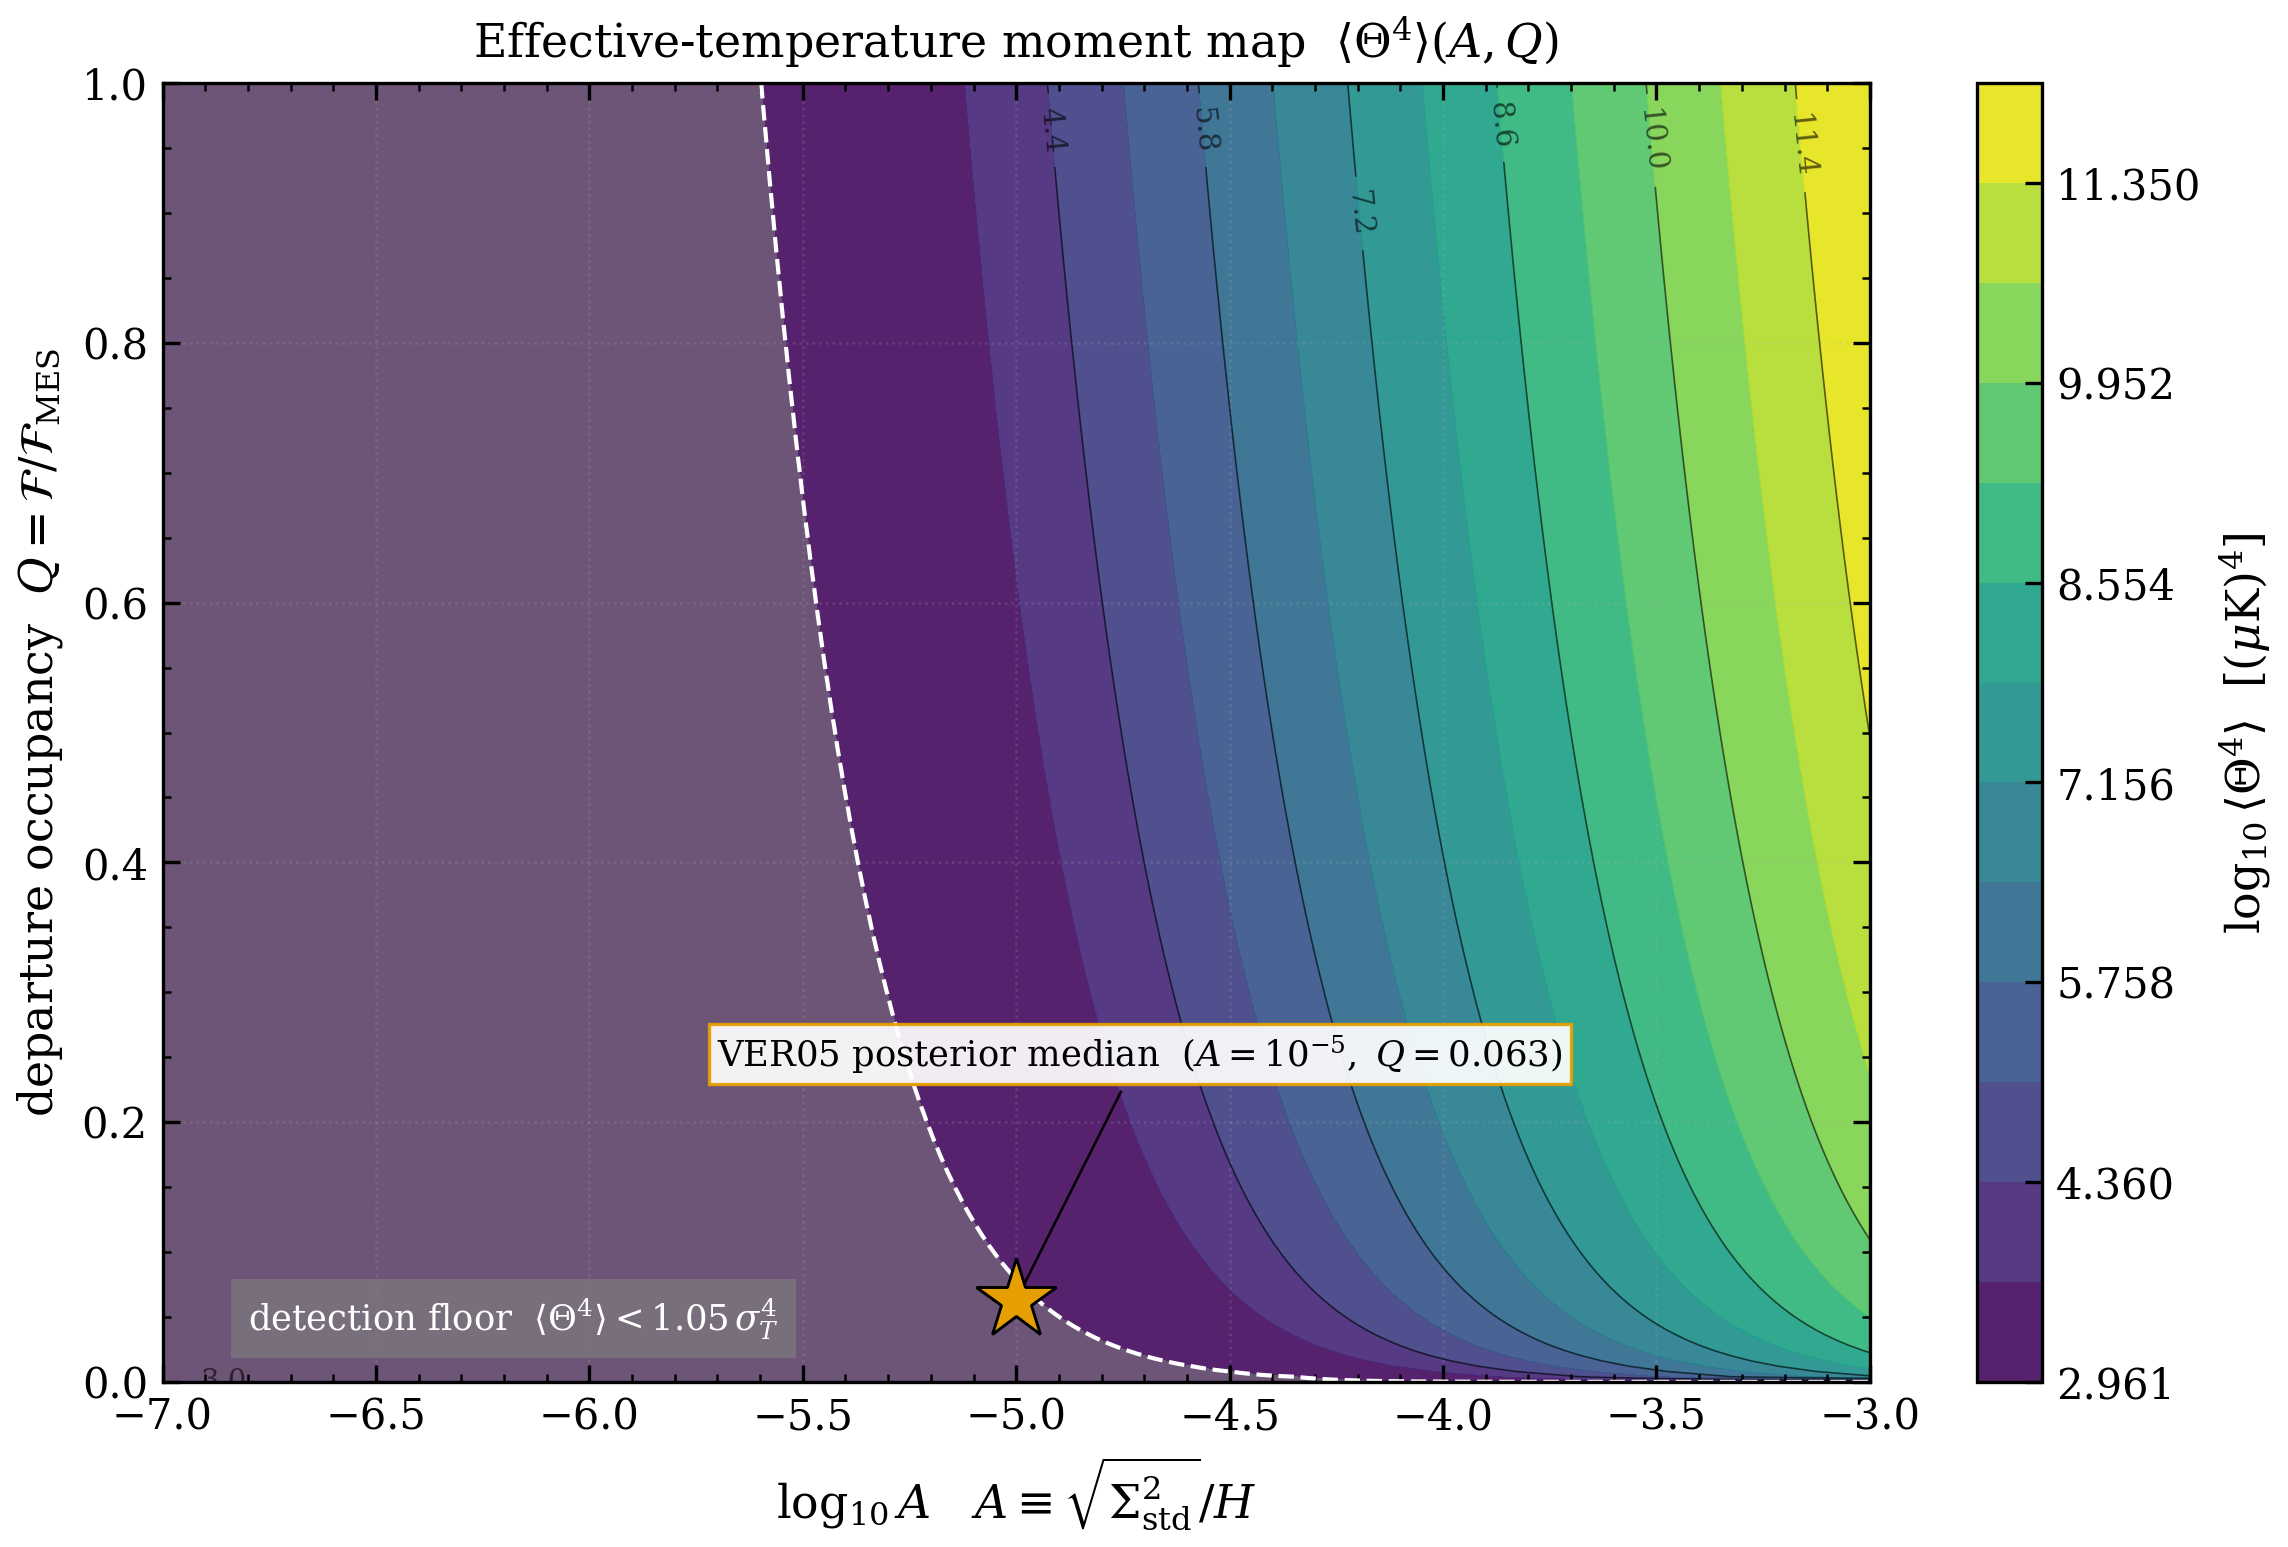
\includegraphics[width=0.82\textwidth,height=0.58\textheight,keepaspectratio]{conditioned_legacy/quarantined-legacy-root-sources__fig_teff_moment_map}
\captionof{figure}{Conditioned legacy diagnostic: teff moment map. Condition: legacy manuscript-generator assumptions. See sidecar manifest for provenance and caveats; appendix-only, not native-transfer or family-ID evidence.}
\label{fig:conditioned-legacy-quarantined-legacy-root-sources-fig-teff-moment-map}
\end{center}

\clearpage
\begin{center}
\centering
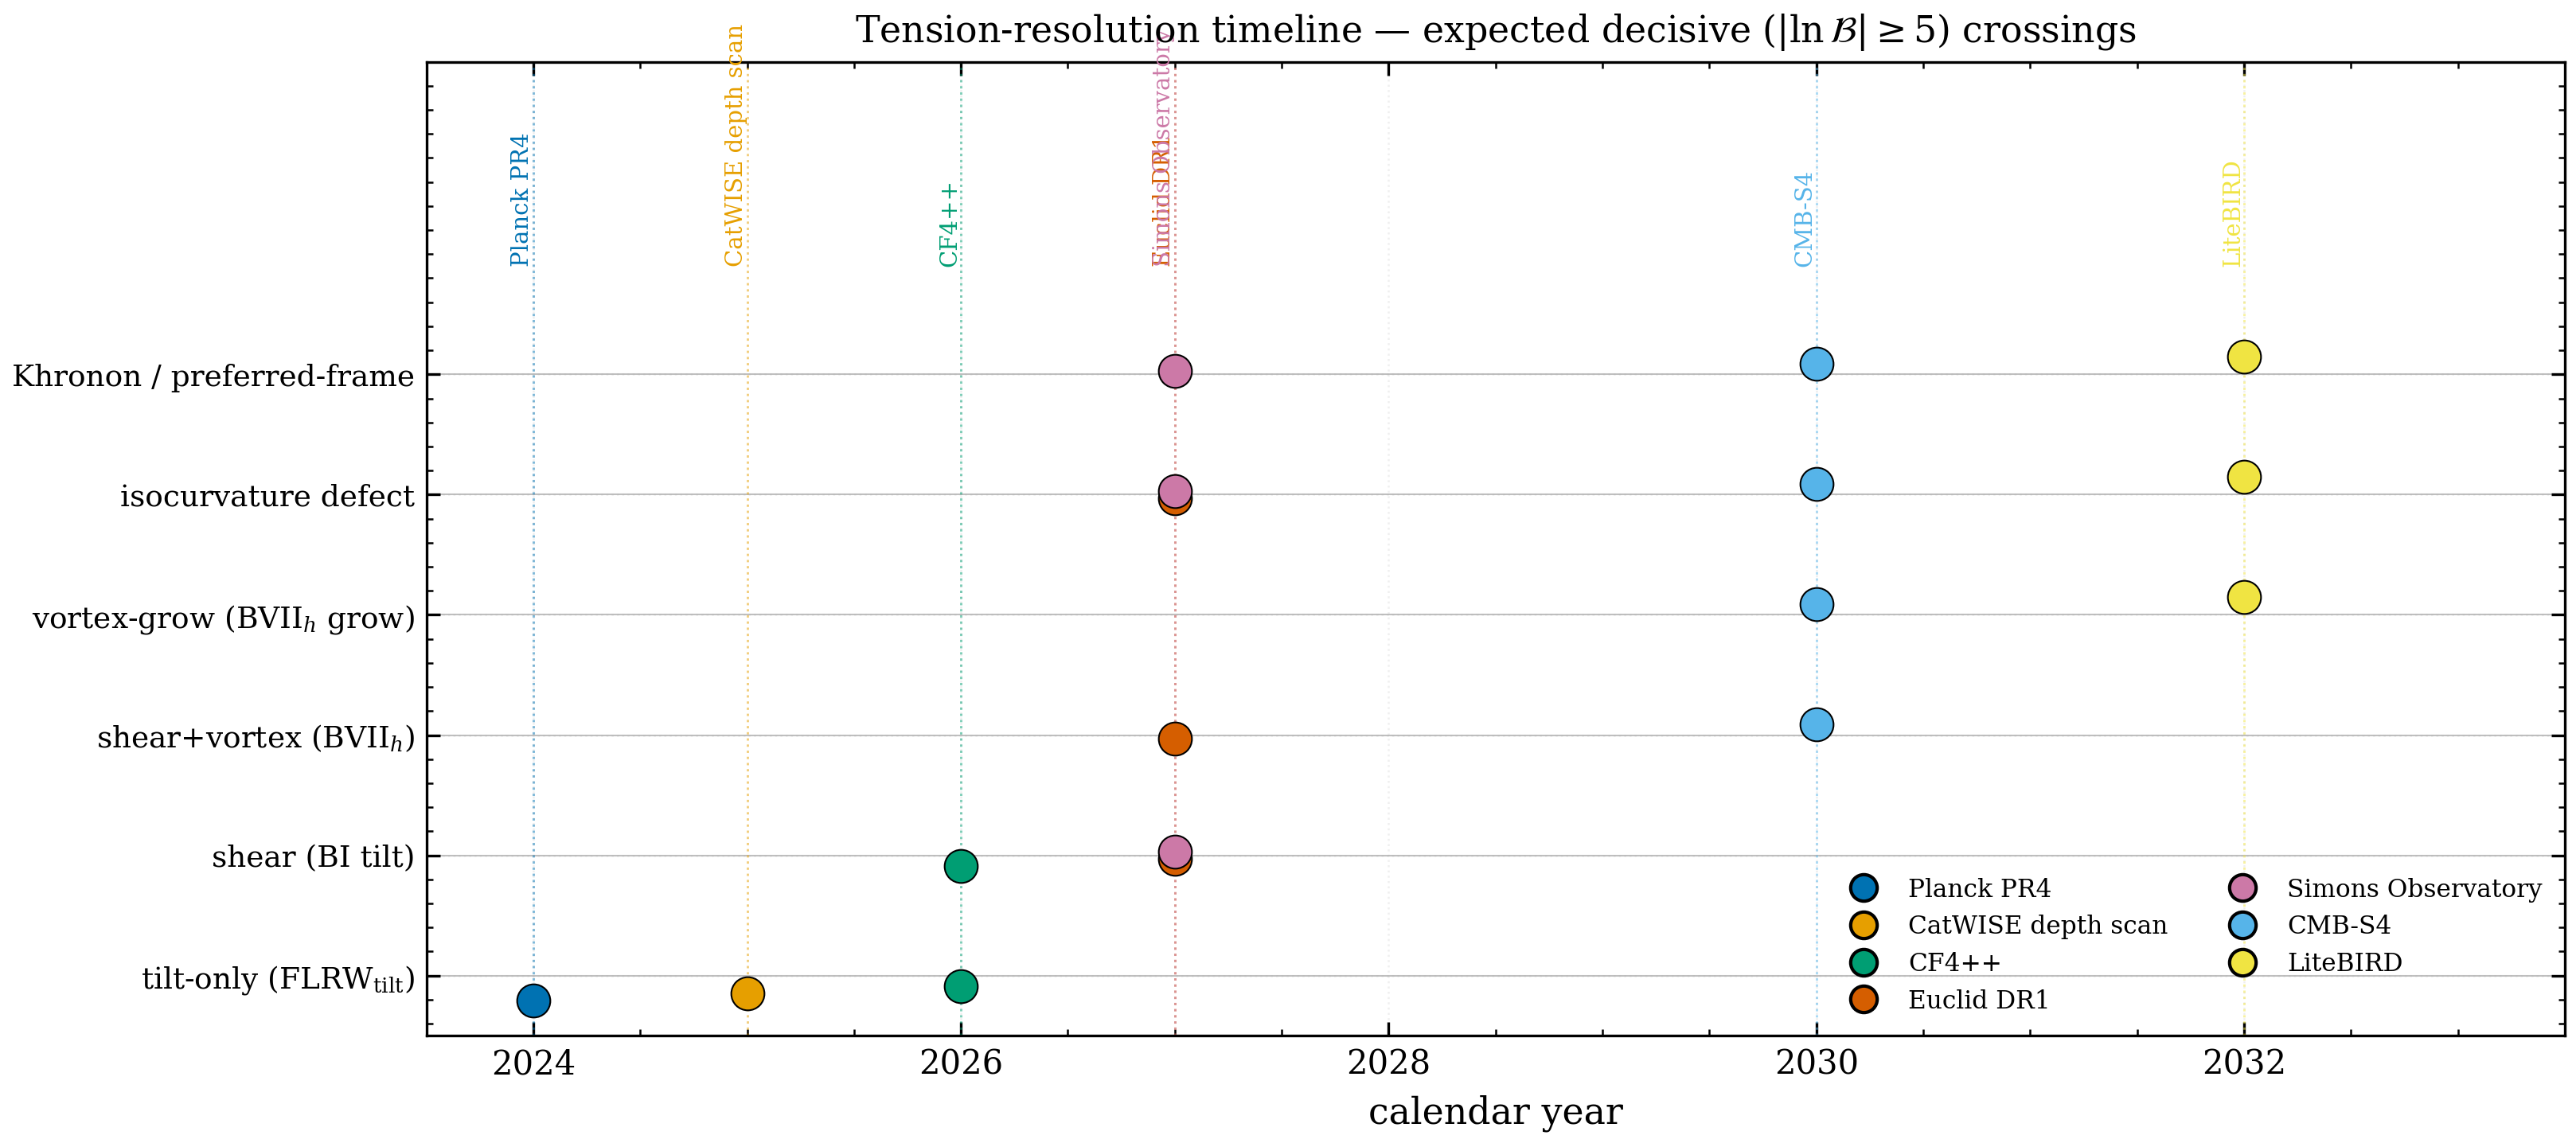
\includegraphics[width=0.82\textwidth,height=0.58\textheight,keepaspectratio]{conditioned_legacy/quarantined-legacy-root-sources__fig_tension_resolution_timeline}
\captionof{figure}{Conditioned legacy diagnostic: tension resolution timeline. Condition: legacy manuscript-generator assumptions. See sidecar manifest for provenance and caveats; appendix-only, not native-transfer or family-ID evidence.}
\label{fig:conditioned-legacy-quarantined-legacy-root-sources-fig-tension-resolution-timeline}
\end{center}

\clearpage
\begin{center}
\centering
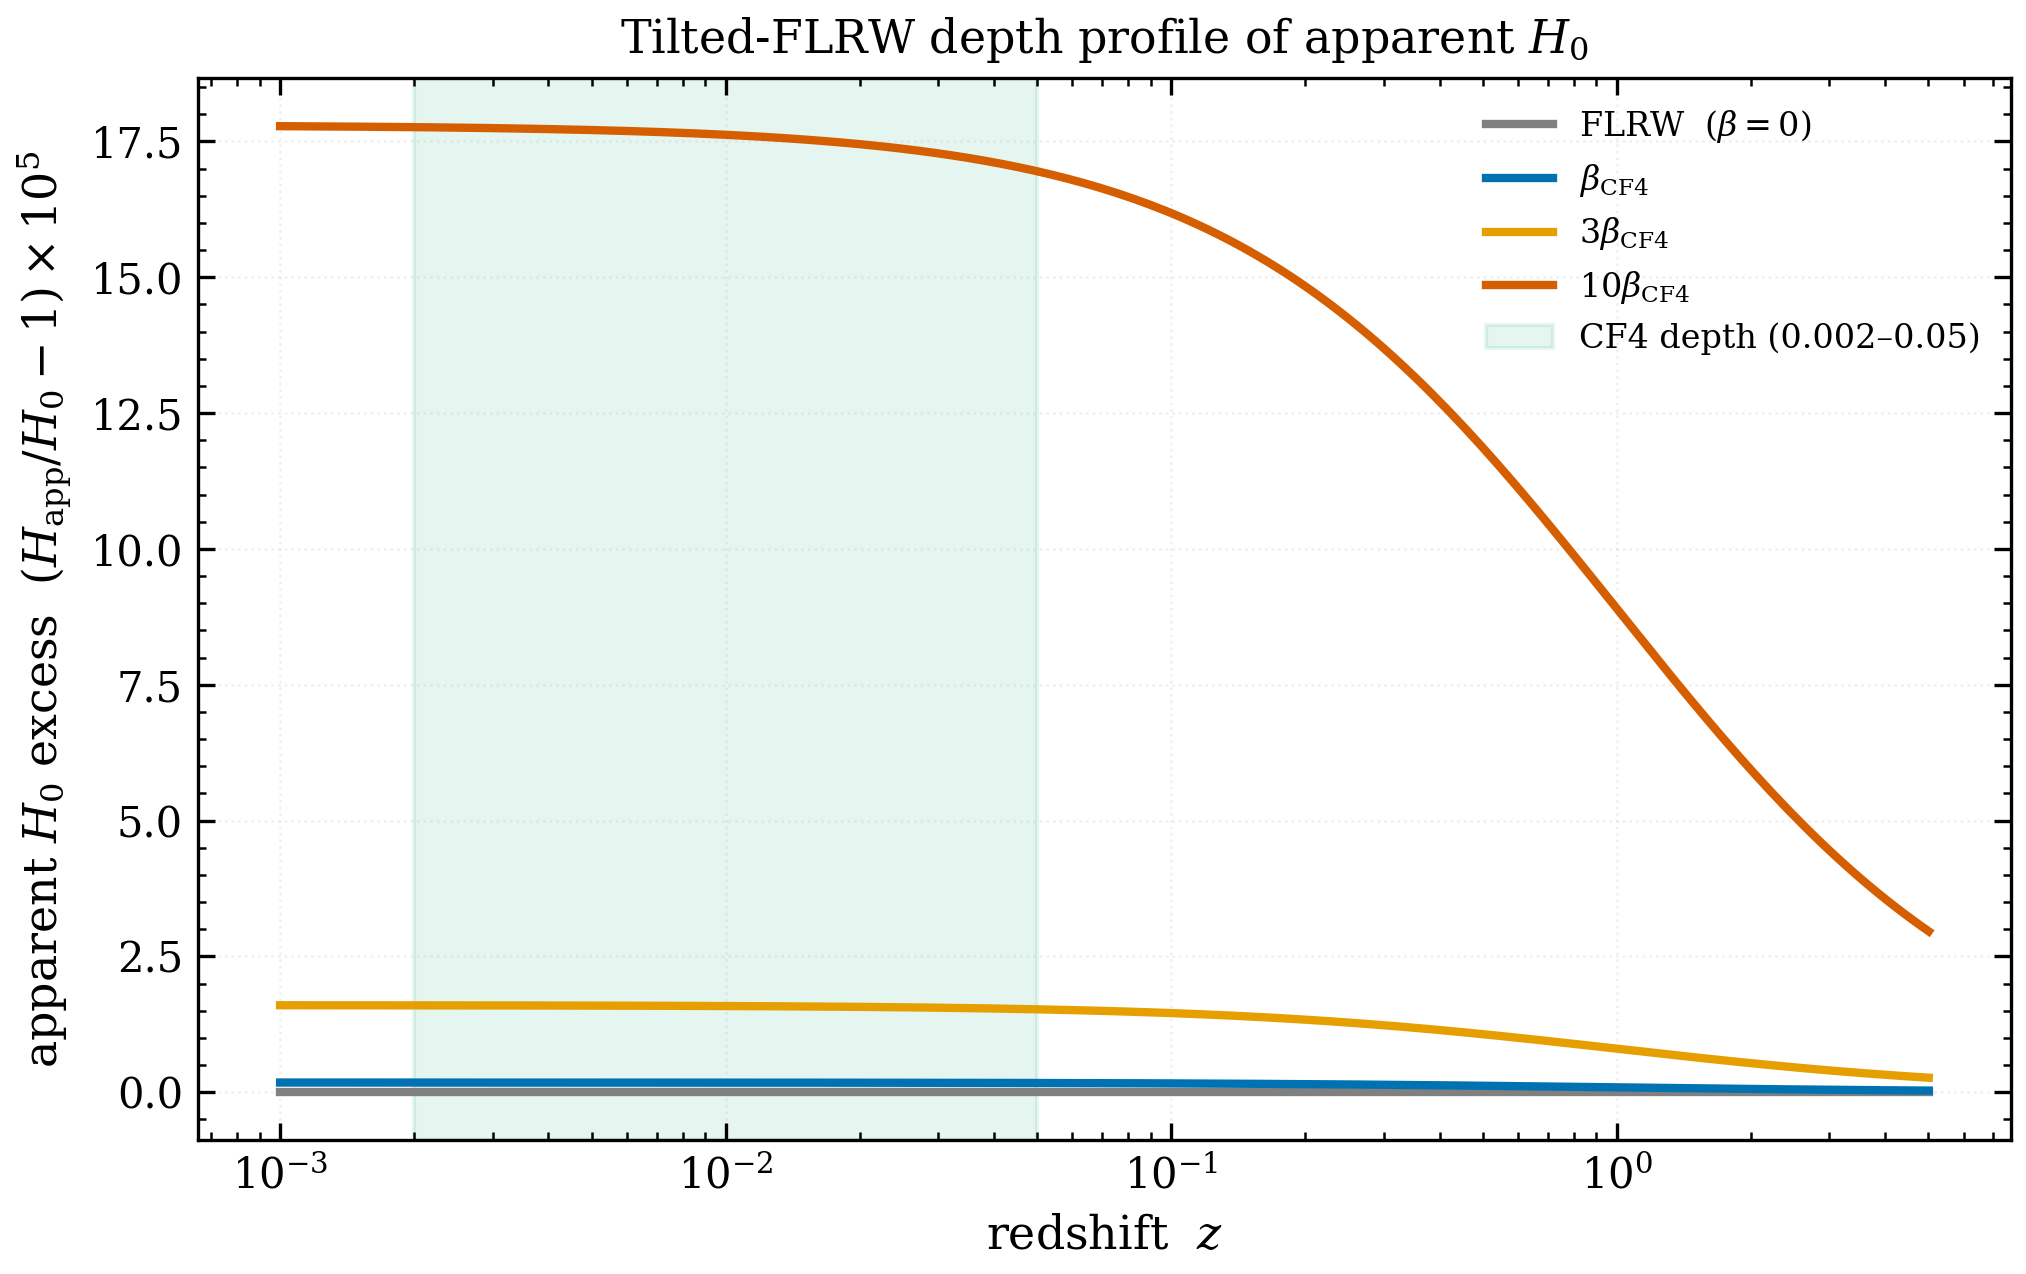
\includegraphics[width=0.82\textwidth,height=0.58\textheight,keepaspectratio]{conditioned_legacy/quarantined-legacy-root-sources__fig_tilted_H0_depth}
\captionof{figure}{Conditioned legacy diagnostic: tilted H0 depth. Condition: legacy manuscript-generator assumptions. See sidecar manifest for provenance and caveats; appendix-only, not native-transfer or family-ID evidence.}
\label{fig:conditioned-legacy-quarantined-legacy-root-sources-fig-tilted-h0-depth}
\end{center}

\clearpage
\begin{center}
\centering
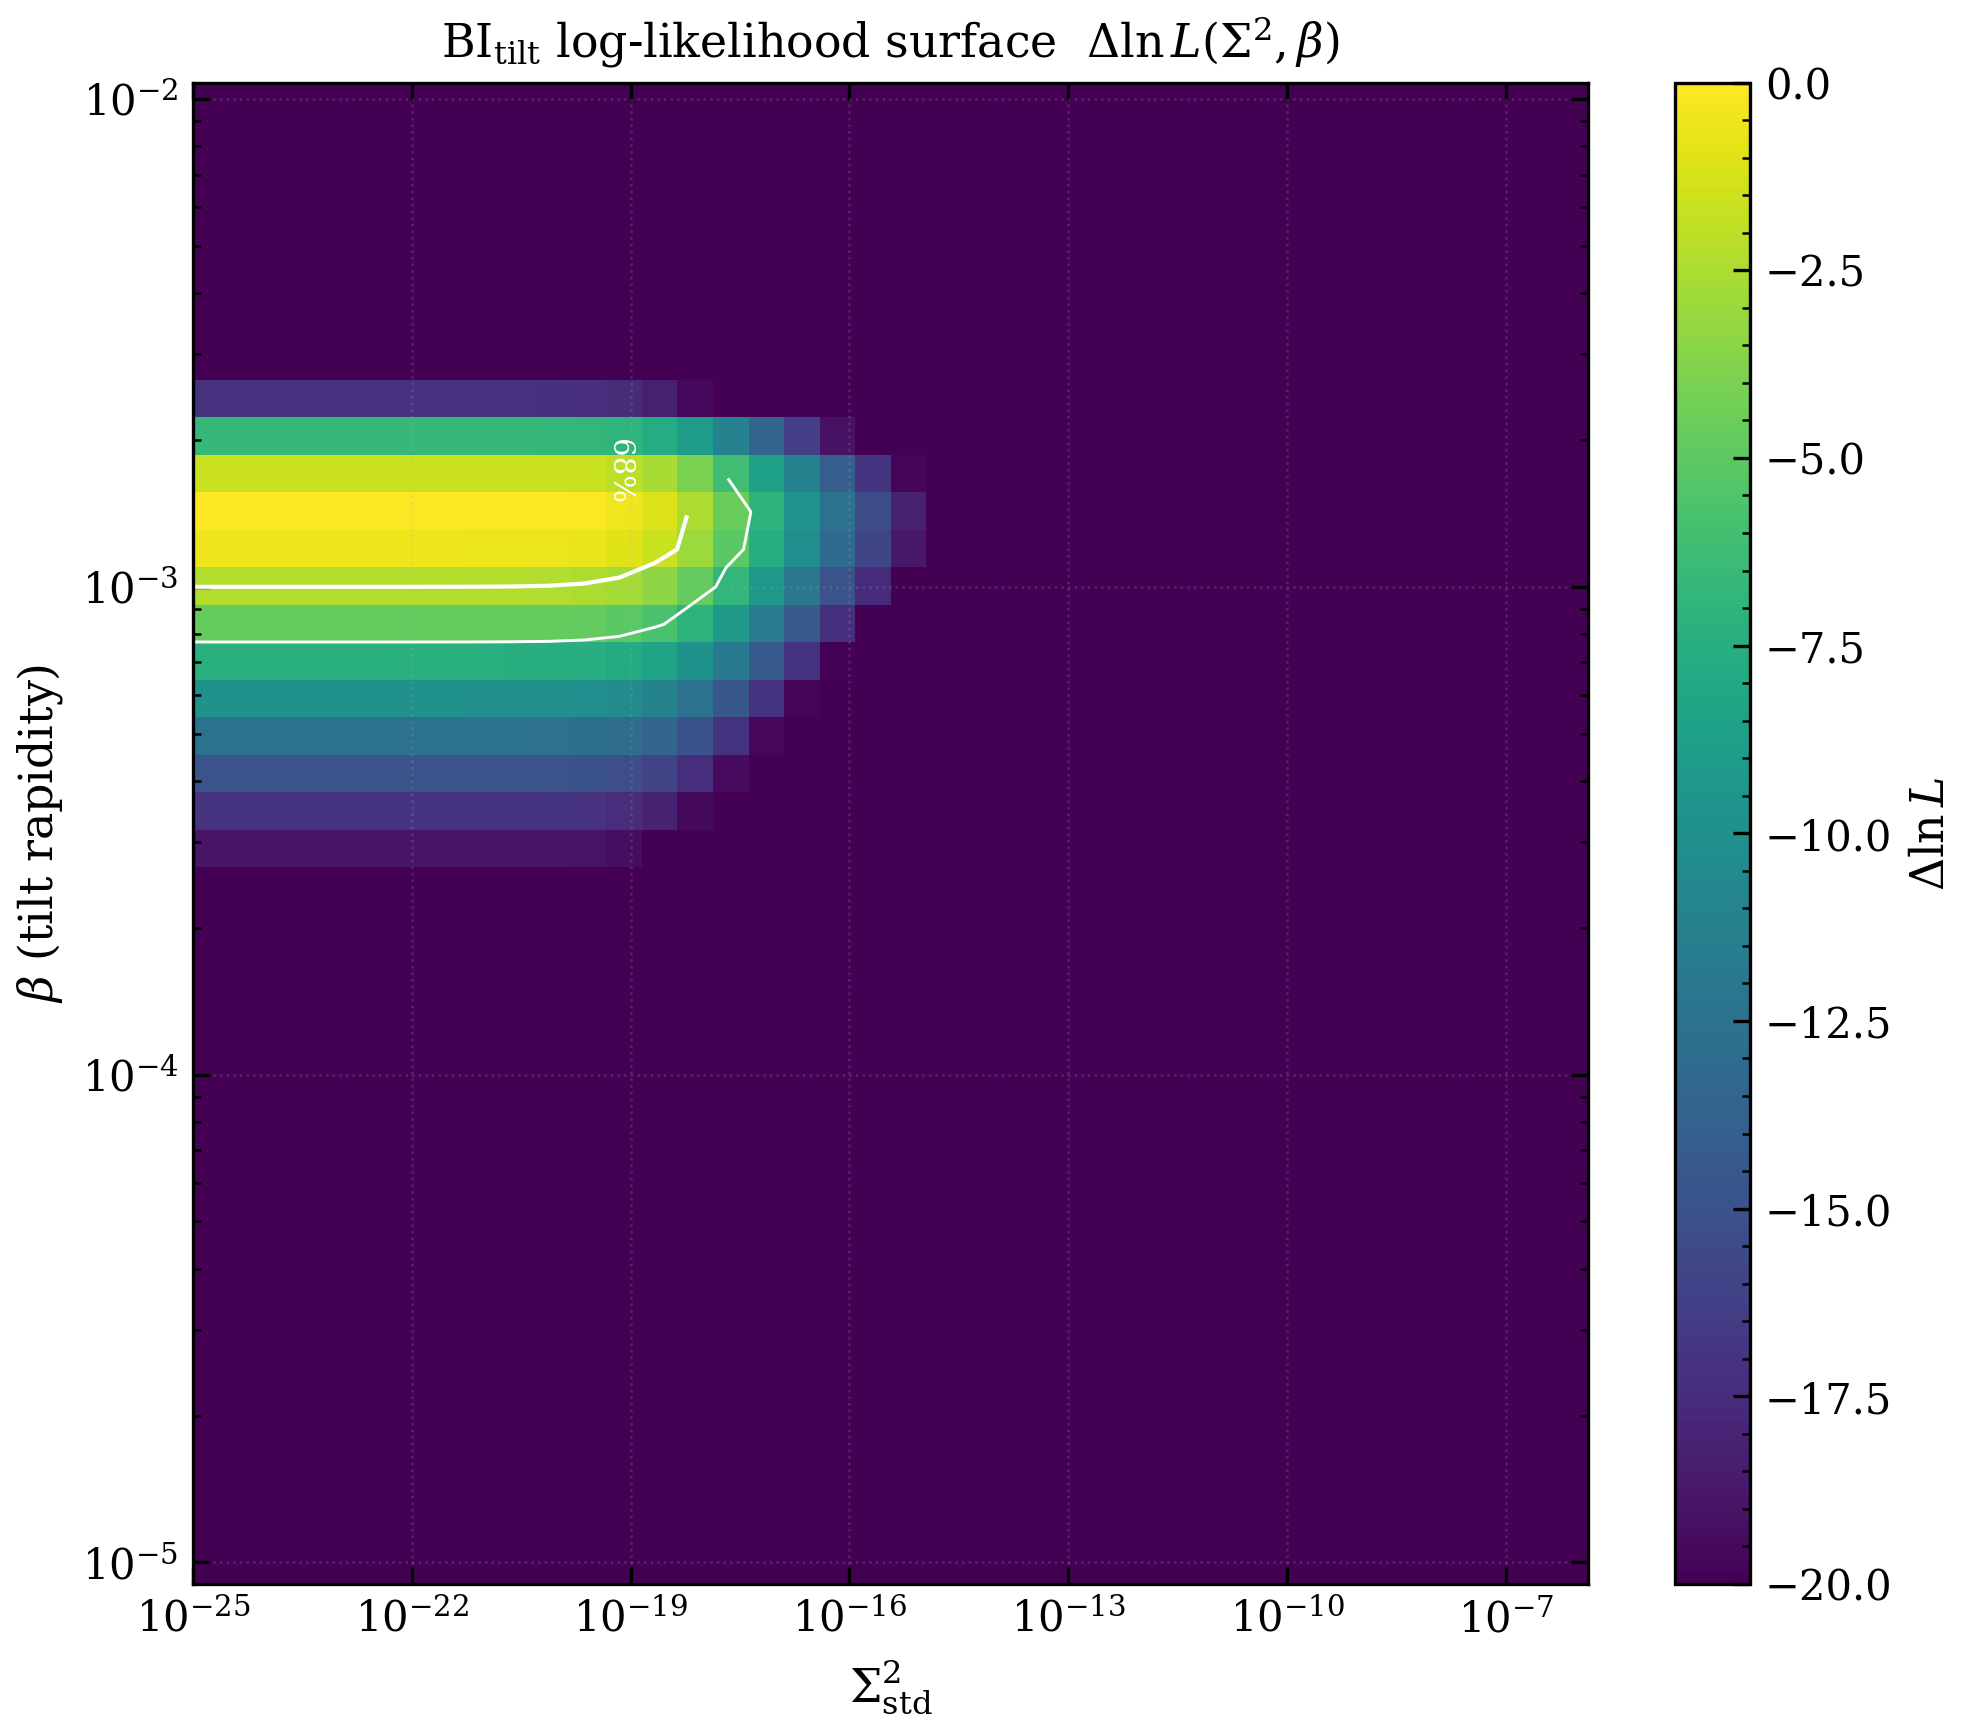
\includegraphics[width=0.82\textwidth,height=0.58\textheight,keepaspectratio]{conditioned_legacy/quarantined-legacy-root-sources__fig_triangle_BI_R03}
\captionof{figure}{Conditioned legacy diagnostic: triangle BI R03. Condition: legacy statistical assumptions without current null/PPC/LOOCV refresh. See sidecar manifest for provenance and caveats; appendix-only, not native-transfer or family-ID evidence.}
\label{fig:conditioned-legacy-quarantined-legacy-root-sources-fig-triangle-bi-r03}
\end{center}

\clearpage
\begin{center}
\centering
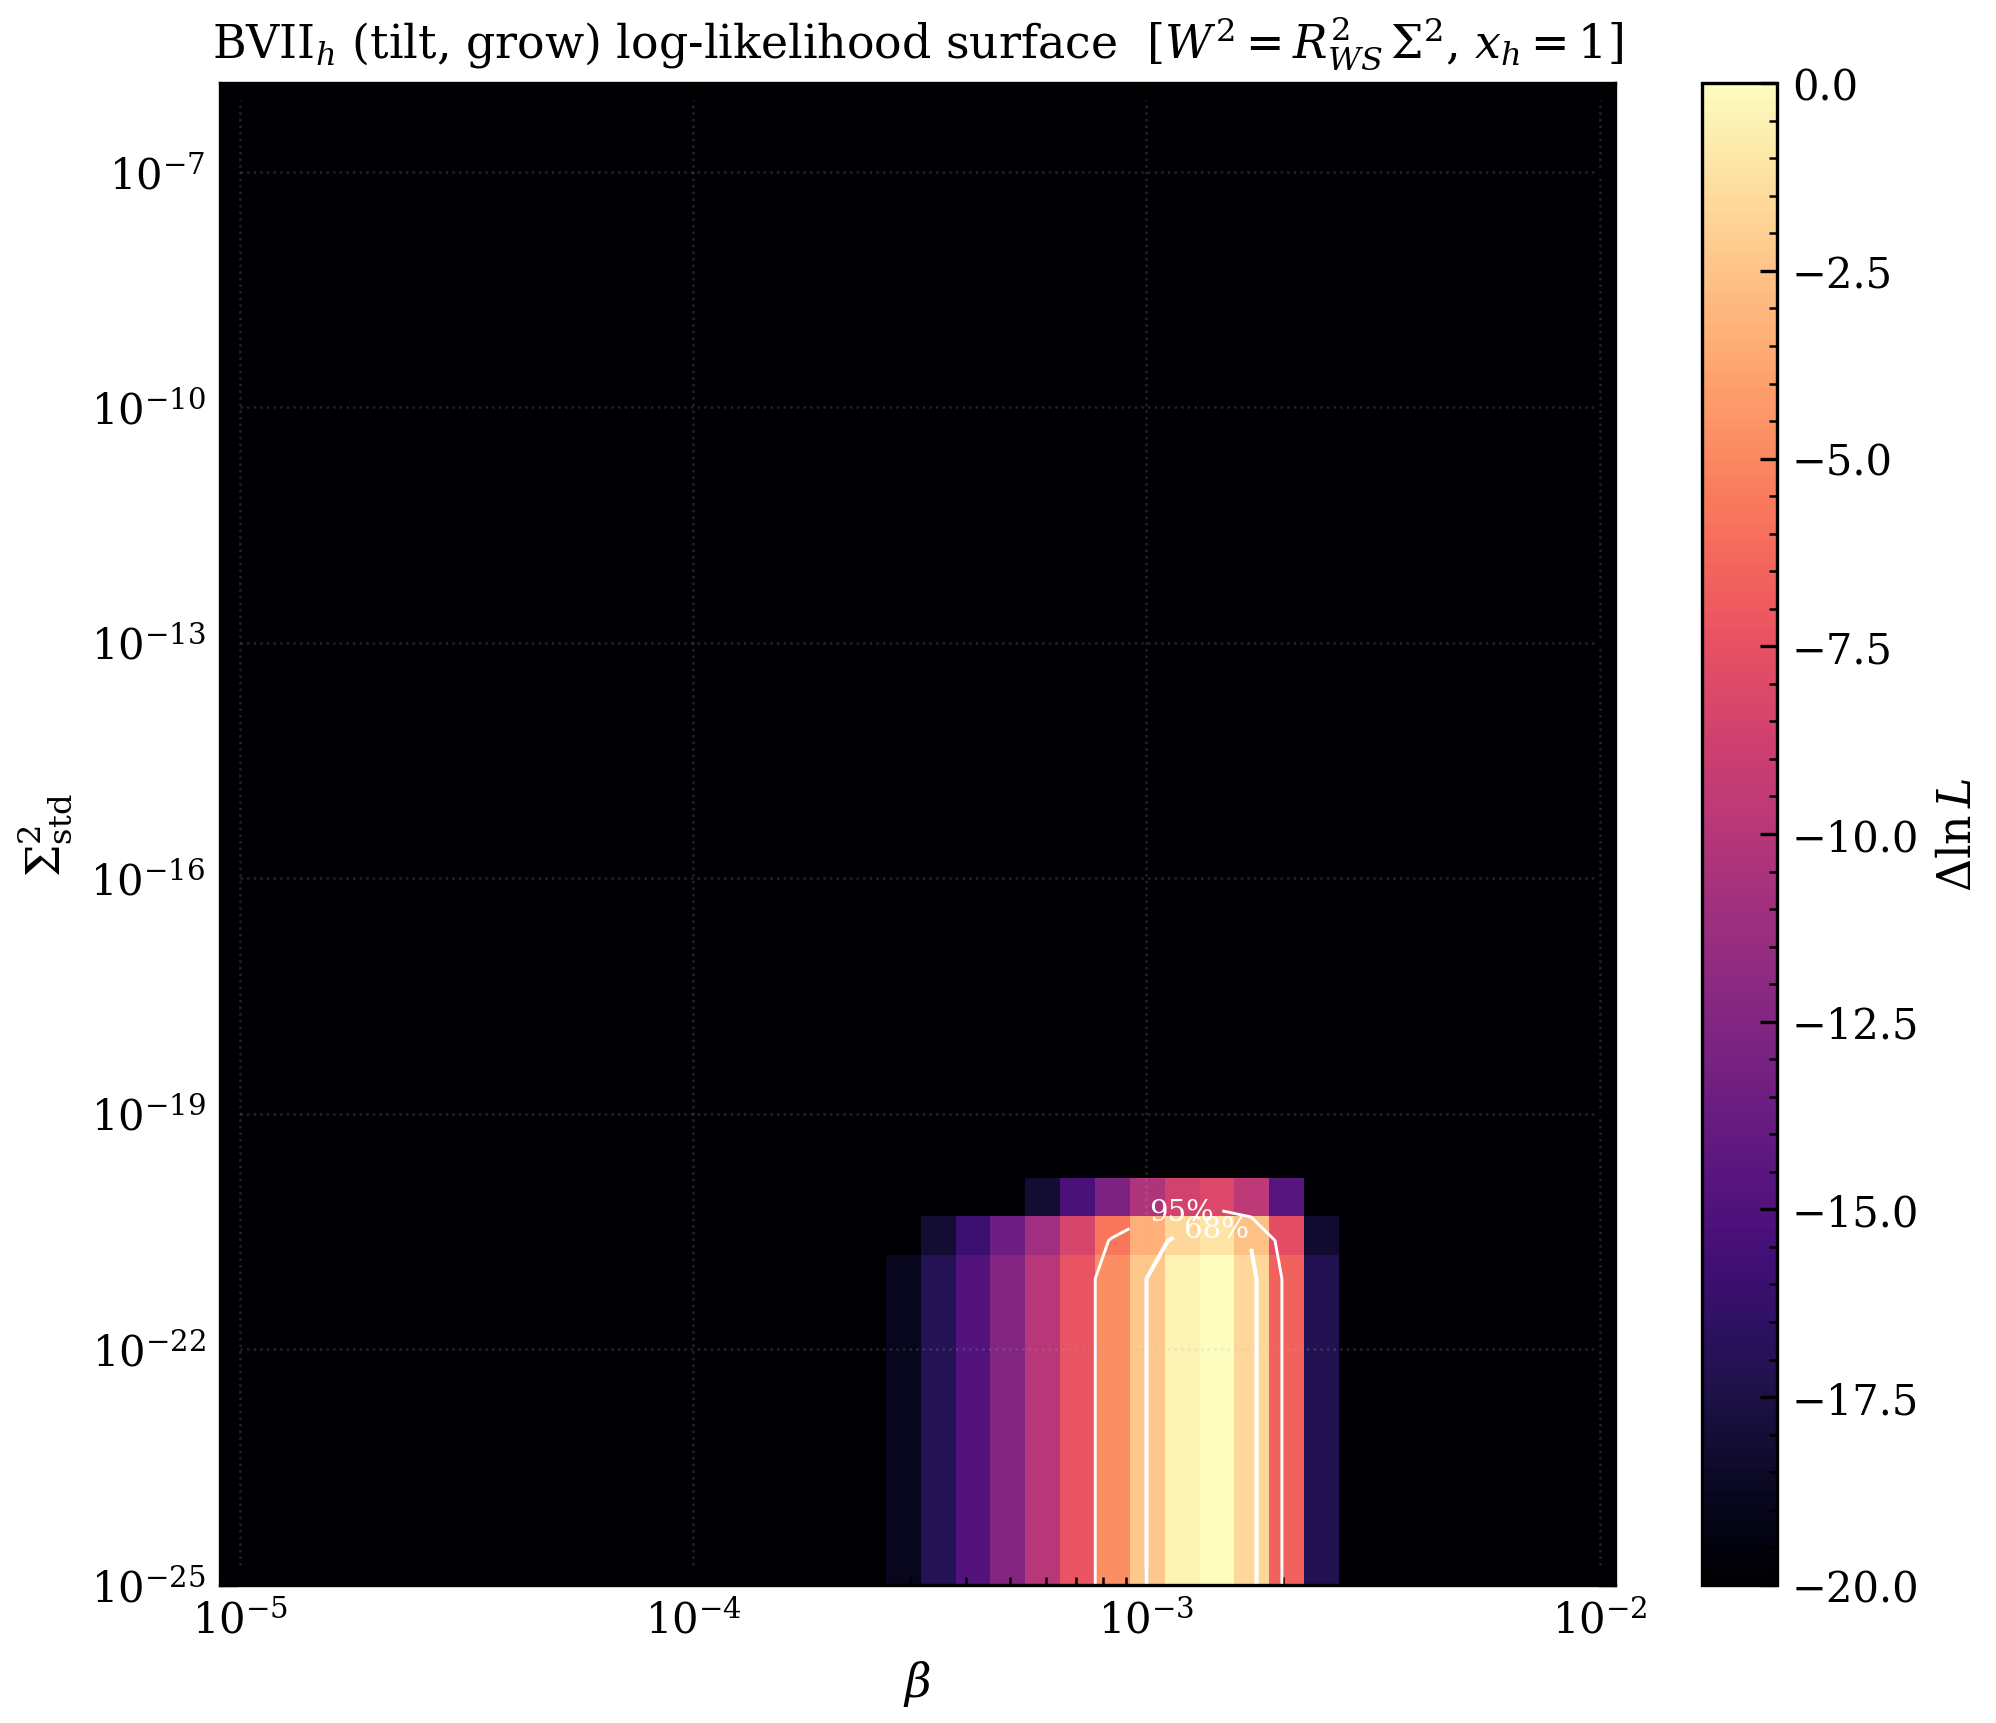
\includegraphics[width=0.82\textwidth,height=0.58\textheight,keepaspectratio]{conditioned_legacy/quarantined-legacy-root-sources__fig_triangle_BVIIh_grow_R03}
\captionof{figure}{Conditioned legacy diagnostic: triangle BVIIh grow R03. Condition: legacy statistical assumptions without current null/PPC/LOOCV refresh. See sidecar manifest for provenance and caveats; appendix-only, not native-transfer or family-ID evidence.}
\label{fig:conditioned-legacy-quarantined-legacy-root-sources-fig-triangle-bviih-grow-r03}
\end{center}

\clearpage
\begin{center}
\centering
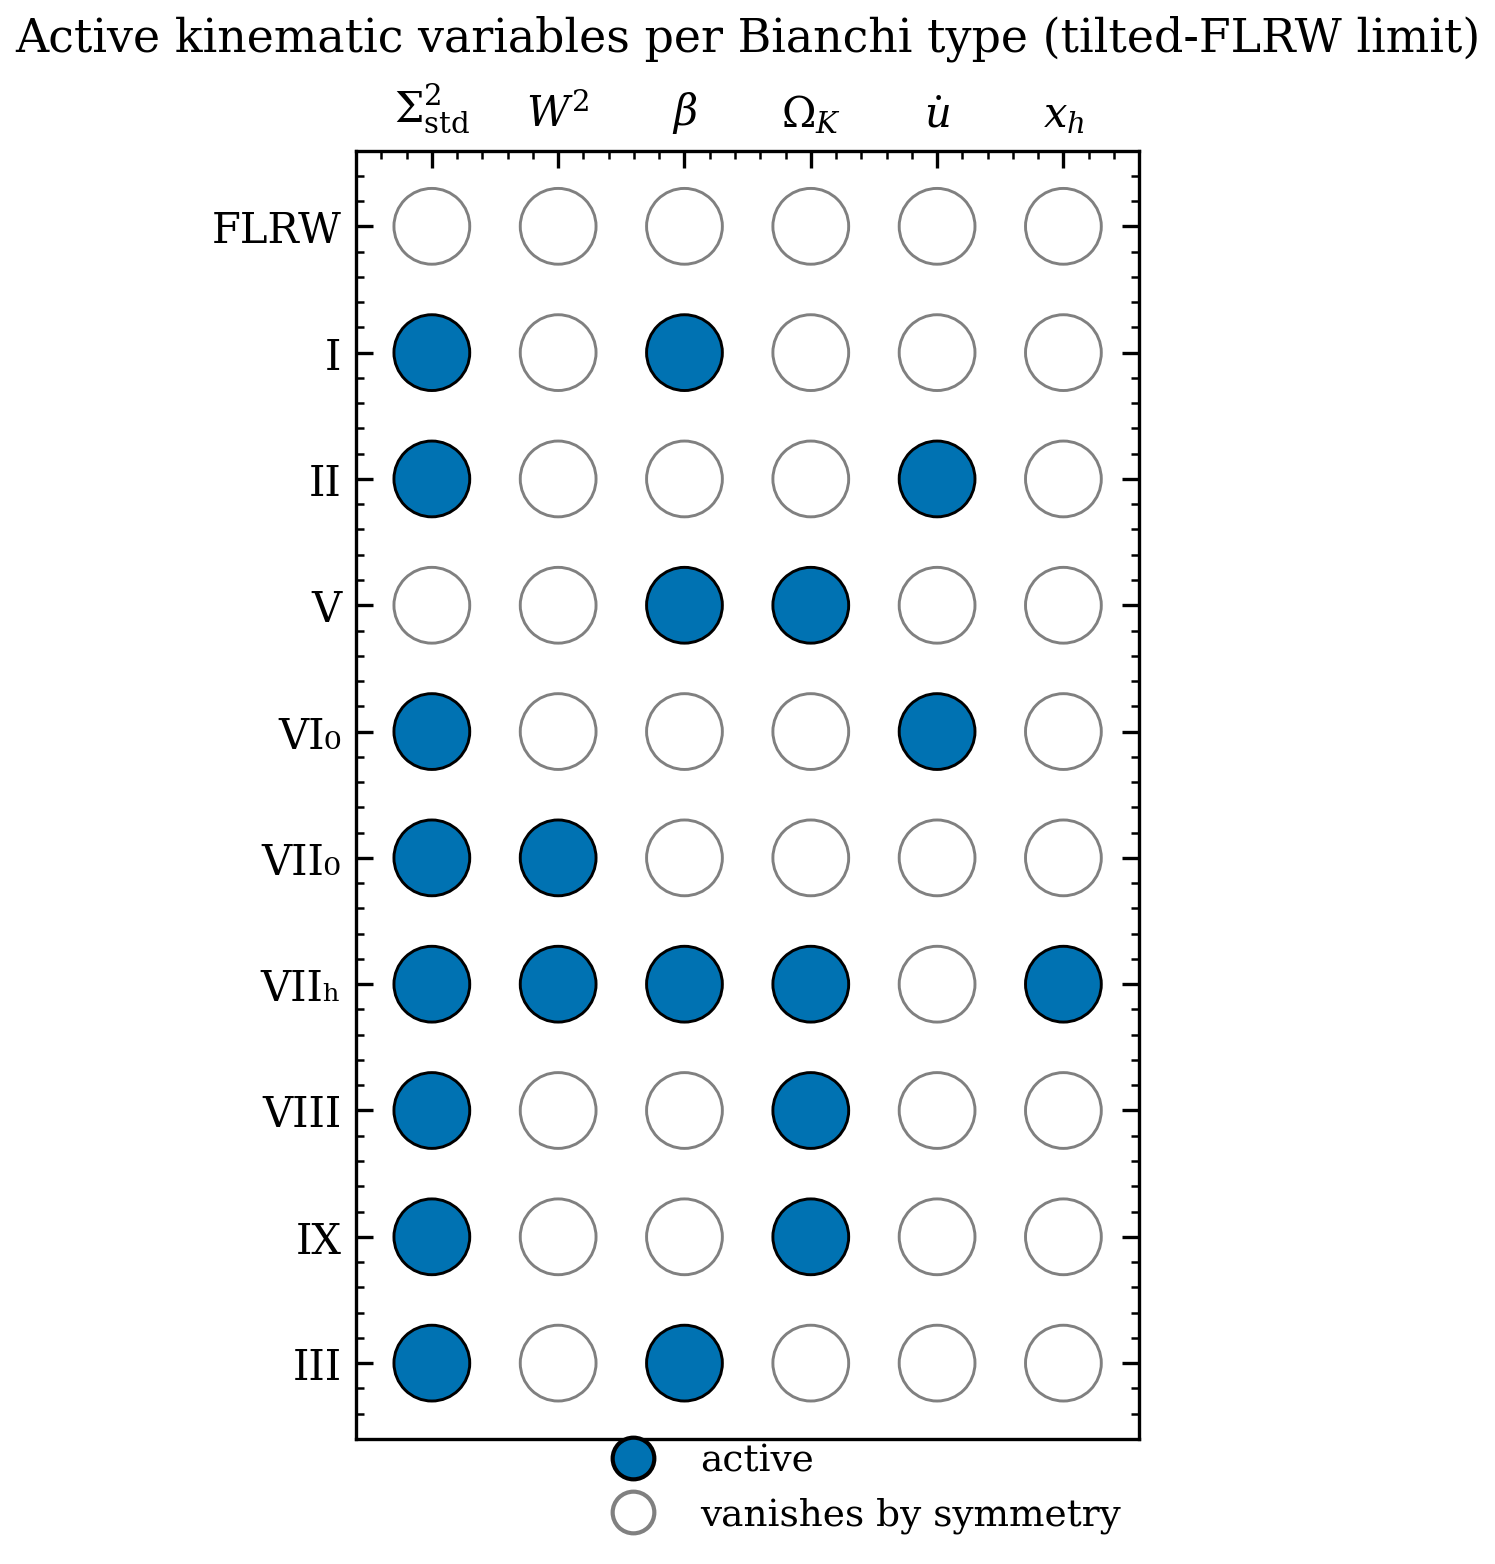
\includegraphics[width=0.82\textwidth,height=0.58\textheight,keepaspectratio]{conditioned_legacy/quarantined-legacy-root-sources__fig_type_by_type_summary}
\captionof{figure}{Conditioned legacy diagnostic: type by type summary. Condition: legacy manuscript-generator assumptions. See sidecar manifest for provenance and caveats; appendix-only, not native-transfer or family-ID evidence.}
\label{fig:conditioned-legacy-quarantined-legacy-root-sources-fig-type-by-type-summary}
\end{center}

\clearpage
\begin{center}
\centering
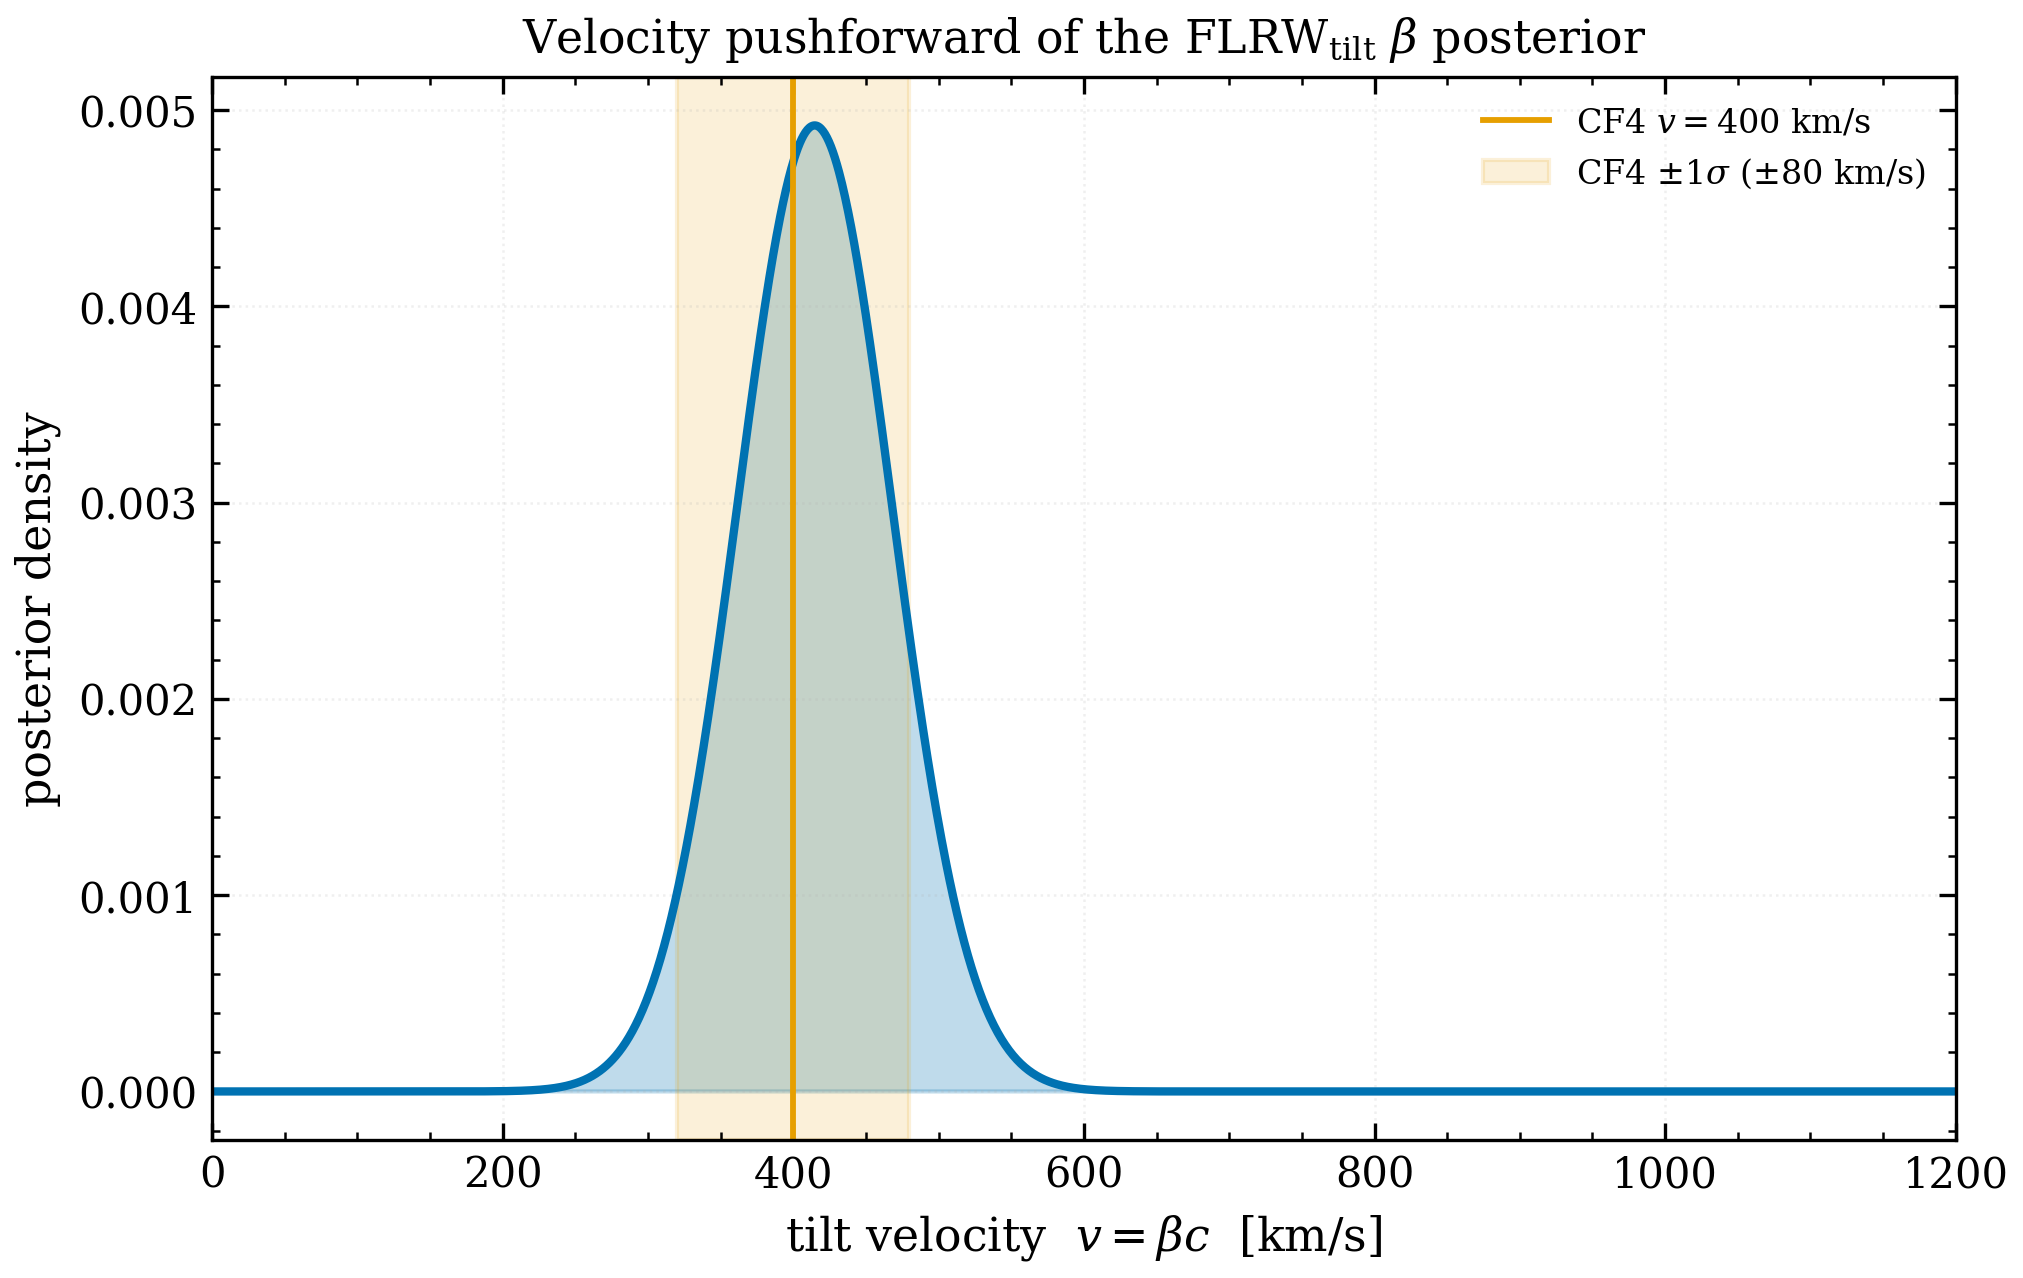
\includegraphics[width=0.82\textwidth,height=0.58\textheight,keepaspectratio]{conditioned_legacy/quarantined-legacy-root-sources__fig_v_pushforward}
\captionof{figure}{Conditioned legacy diagnostic: v pushforward. Condition: legacy manuscript-generator assumptions. See sidecar manifest for provenance and caveats; appendix-only, not native-transfer or family-ID evidence.}
\label{fig:conditioned-legacy-quarantined-legacy-root-sources-fig-v-pushforward}
\end{center}

\clearpage
\begin{center}
\centering
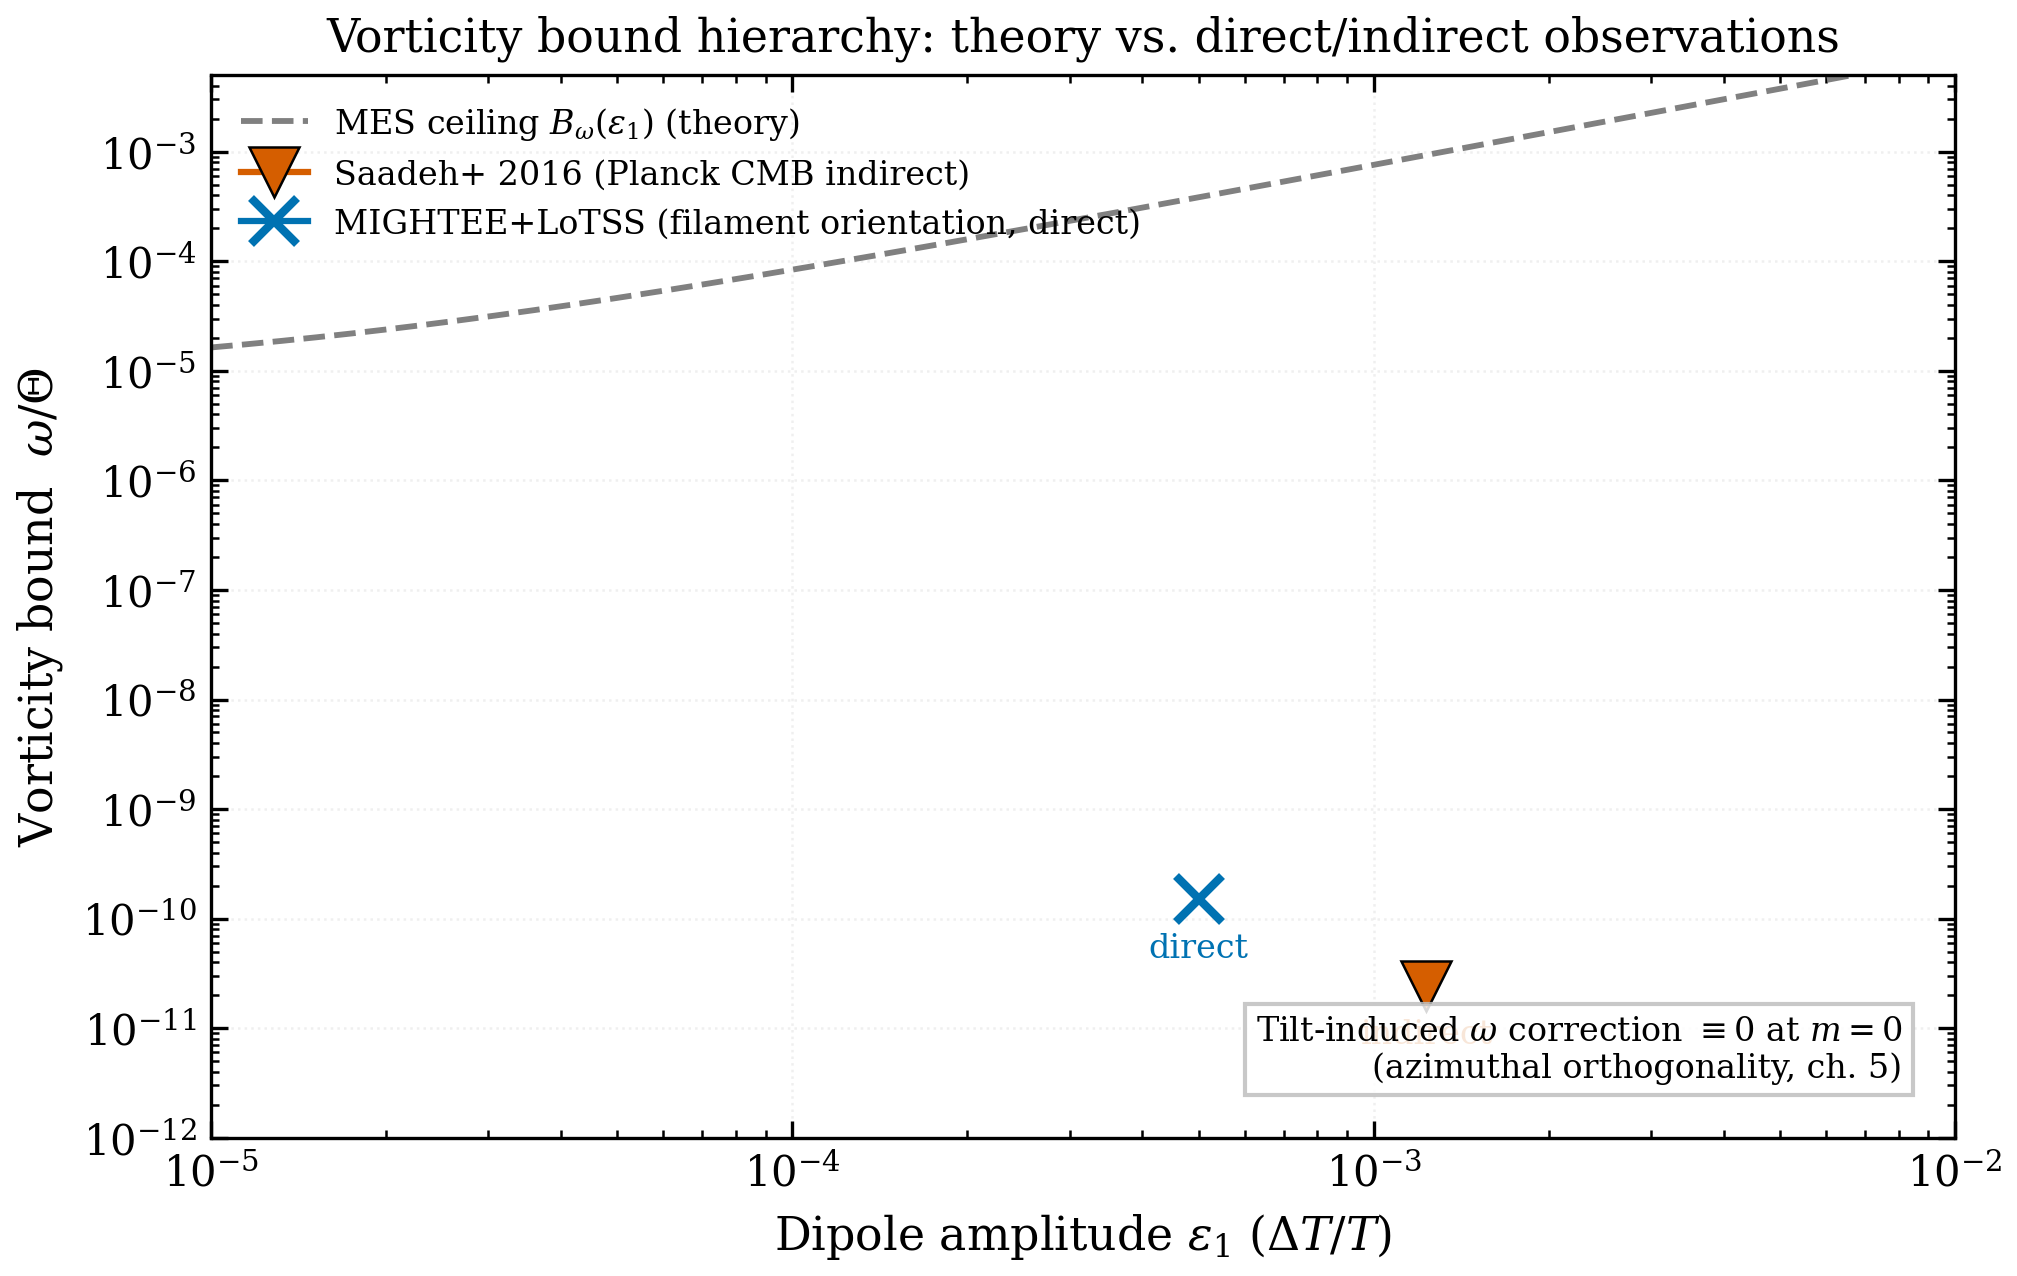
\includegraphics[width=0.82\textwidth,height=0.58\textheight,keepaspectratio]{conditioned_legacy/quarantined-legacy-root-sources__fig_vorticity_hierarchy}
\captionof{figure}{Conditioned legacy diagnostic: vorticity hierarchy. Condition: legacy manuscript-generator assumptions. See sidecar manifest for provenance and caveats; appendix-only, not native-transfer or family-ID evidence.}
\label{fig:conditioned-legacy-quarantined-legacy-root-sources-fig-vorticity-hierarchy}
\end{center}

\clearpage
\begin{center}
\centering
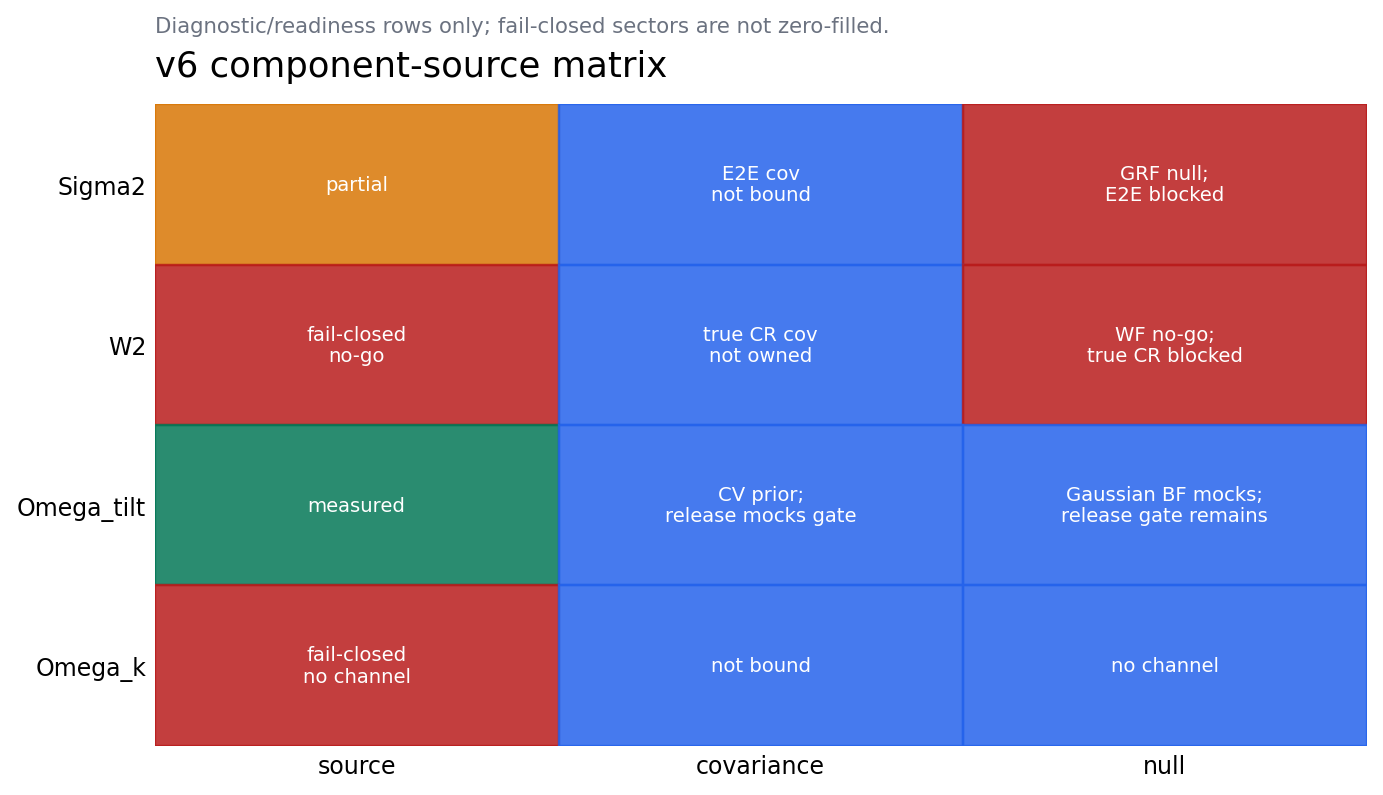
\includegraphics[width=0.82\textwidth,height=0.58\textheight,keepaspectratio]{conditioned_legacy/quarantined-meta-v6-no-download__fig_v6_component_source_matrix}
\captionof{figure}{Conditioned legacy diagnostic: v6 component source matrix. Condition: legacy manuscript-generator assumptions. See sidecar manifest for provenance and caveats; appendix-only, not native-transfer or family-ID evidence.}
\label{fig:conditioned-legacy-quarantined-meta-v6-no-download-fig-v6-component-source-matrix}
\end{center}

\clearpage
\begin{center}
\centering
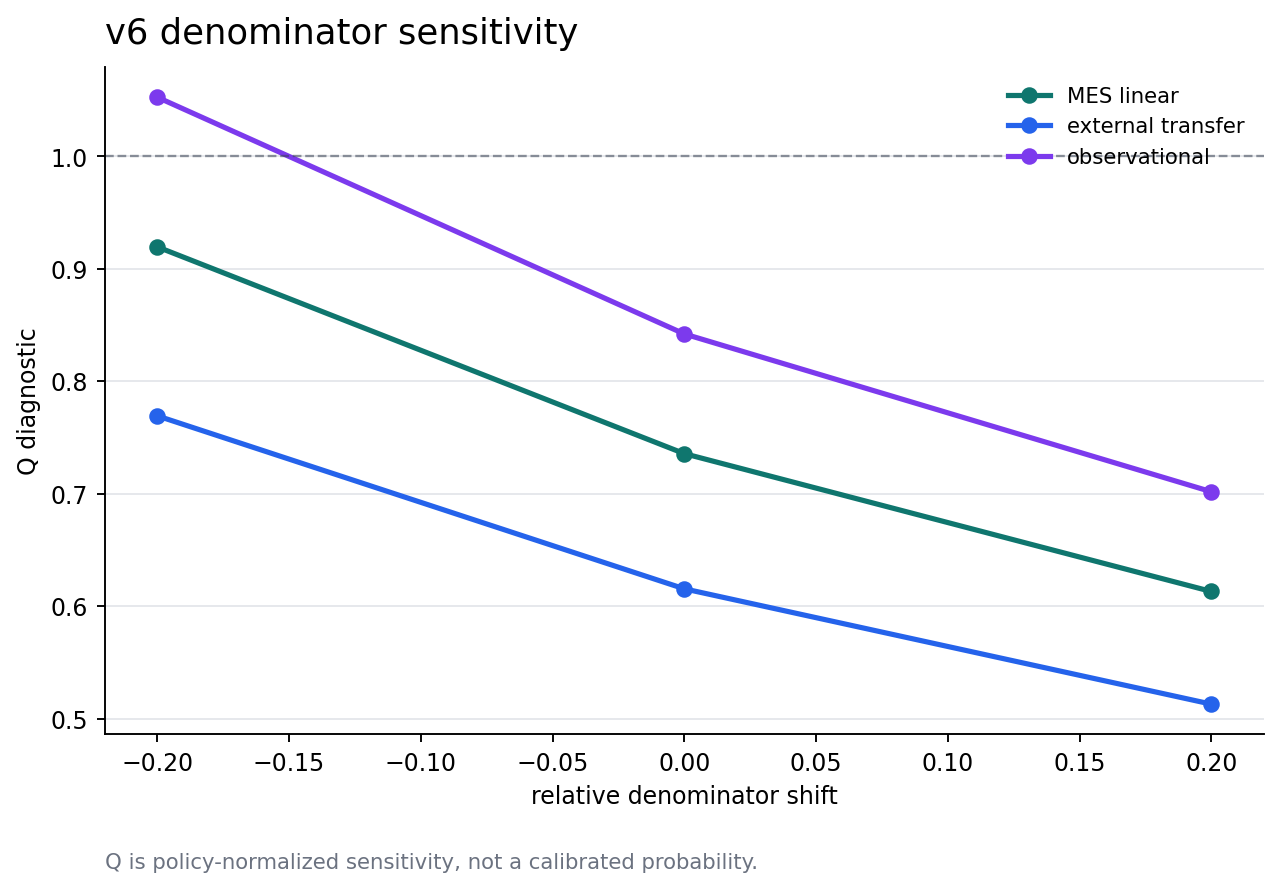
\includegraphics[width=0.82\textwidth,height=0.58\textheight,keepaspectratio]{conditioned_legacy/quarantined-meta-v6-no-download__fig_v6_denominator_sensitivity}
\captionof{figure}{Conditioned legacy diagnostic: v6 denominator sensitivity. Condition: legacy manuscript-generator assumptions. See sidecar manifest for provenance and caveats; appendix-only, not native-transfer or family-ID evidence.}
\label{fig:conditioned-legacy-quarantined-meta-v6-no-download-fig-v6-denominator-sensitivity}
\end{center}

\clearpage
\begin{center}
\centering
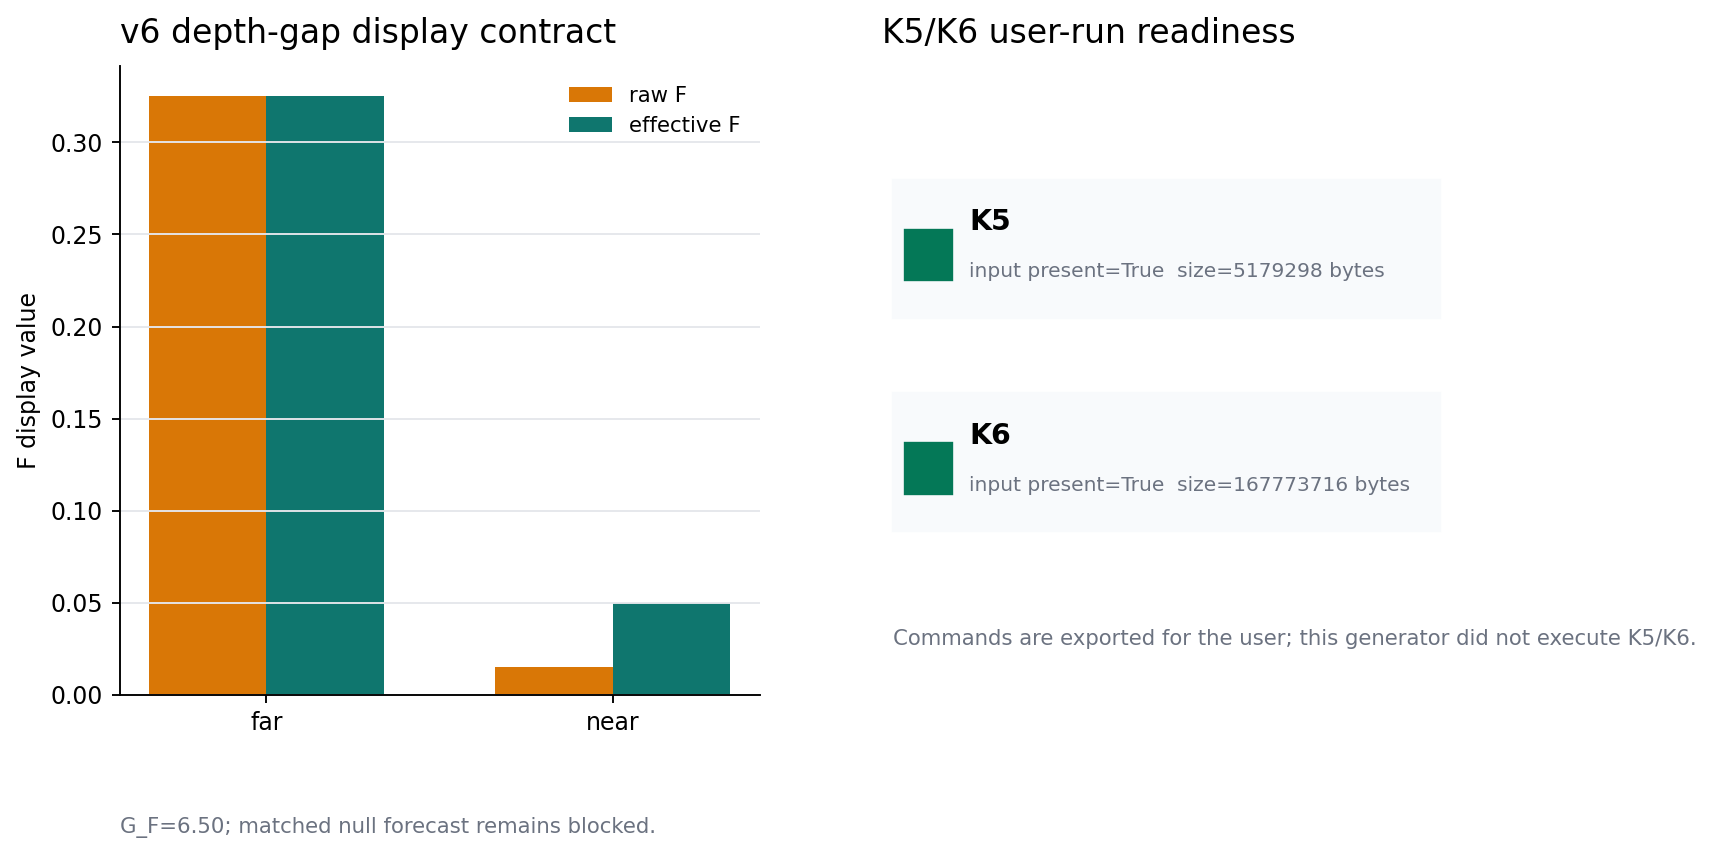
\includegraphics[width=0.82\textwidth,height=0.58\textheight,keepaspectratio]{conditioned_legacy/quarantined-meta-v6-no-download__fig_v6_depth_gap_and_readiness}
\captionof{figure}{Conditioned legacy diagnostic: v6 depth gap and readiness. Condition: legacy manuscript-generator assumptions. See sidecar manifest for provenance and caveats; appendix-only, not native-transfer or family-ID evidence.}
\label{fig:conditioned-legacy-quarantined-meta-v6-no-download-fig-v6-depth-gap-and-readiness}
\end{center}

\clearpage
\begin{center}
\centering
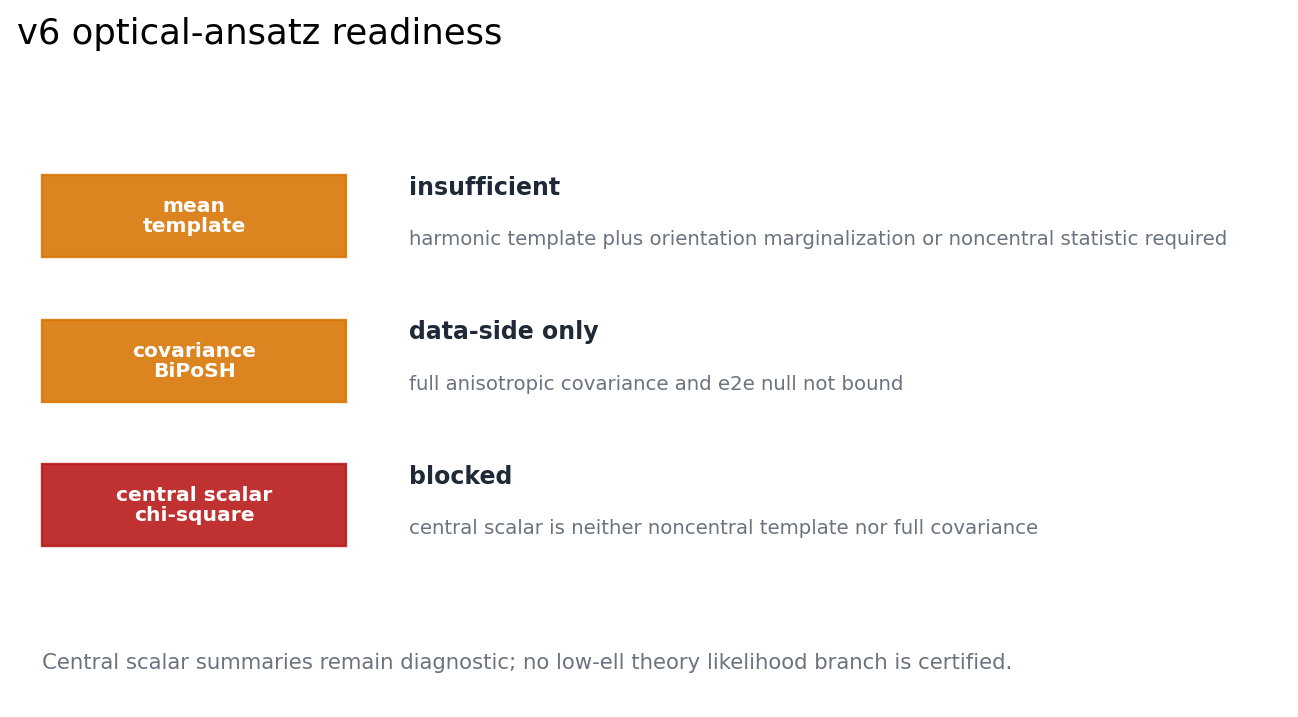
\includegraphics[width=0.82\textwidth,height=0.58\textheight,keepaspectratio]{conditioned_legacy/quarantined-meta-v6-no-download__fig_v6_optical_ansatz_readiness}
\captionof{figure}{Conditioned legacy diagnostic: v6 optical ansatz readiness. Condition: legacy manuscript-generator assumptions. See sidecar manifest for provenance and caveats; appendix-only, not native-transfer or family-ID evidence.}
\label{fig:conditioned-legacy-quarantined-meta-v6-no-download-fig-v6-optical-ansatz-readiness}
\end{center}

\clearpage
\begin{center}
\centering
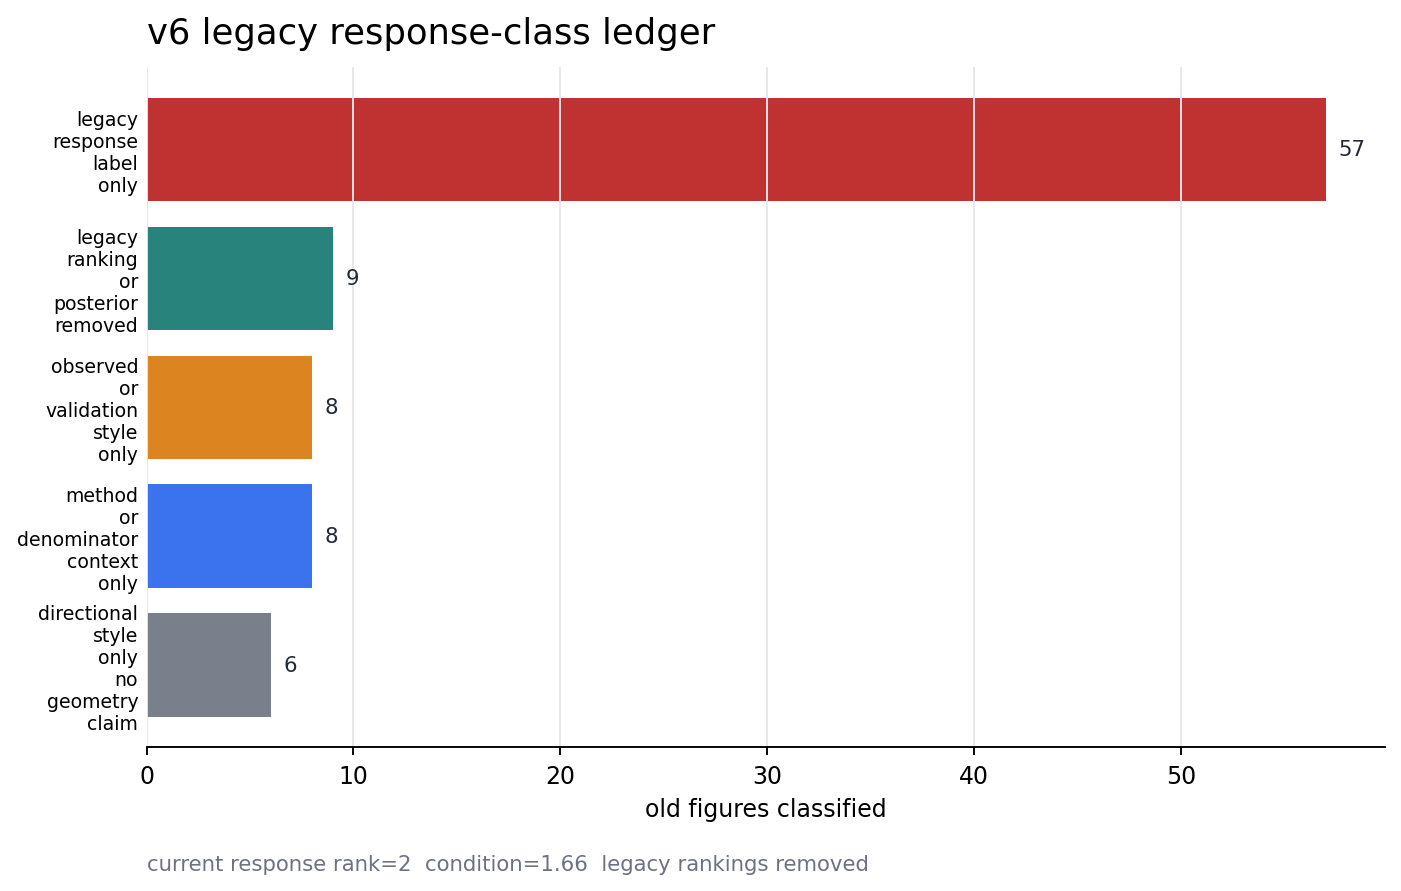
\includegraphics[width=0.82\textwidth,height=0.58\textheight,keepaspectratio]{conditioned_legacy/quarantined-meta-v6-no-download__fig_v6_response_class_ledger}
\captionof{figure}{Conditioned legacy diagnostic: v6 response class ledger. Condition: legacy manuscript-generator assumptions. See sidecar manifest for provenance and caveats; appendix-only, not native-transfer or family-ID evidence.}
\label{fig:conditioned-legacy-quarantined-meta-v6-no-download-fig-v6-response-class-ledger}
\end{center}

\clearpage
\begin{center}
\centering
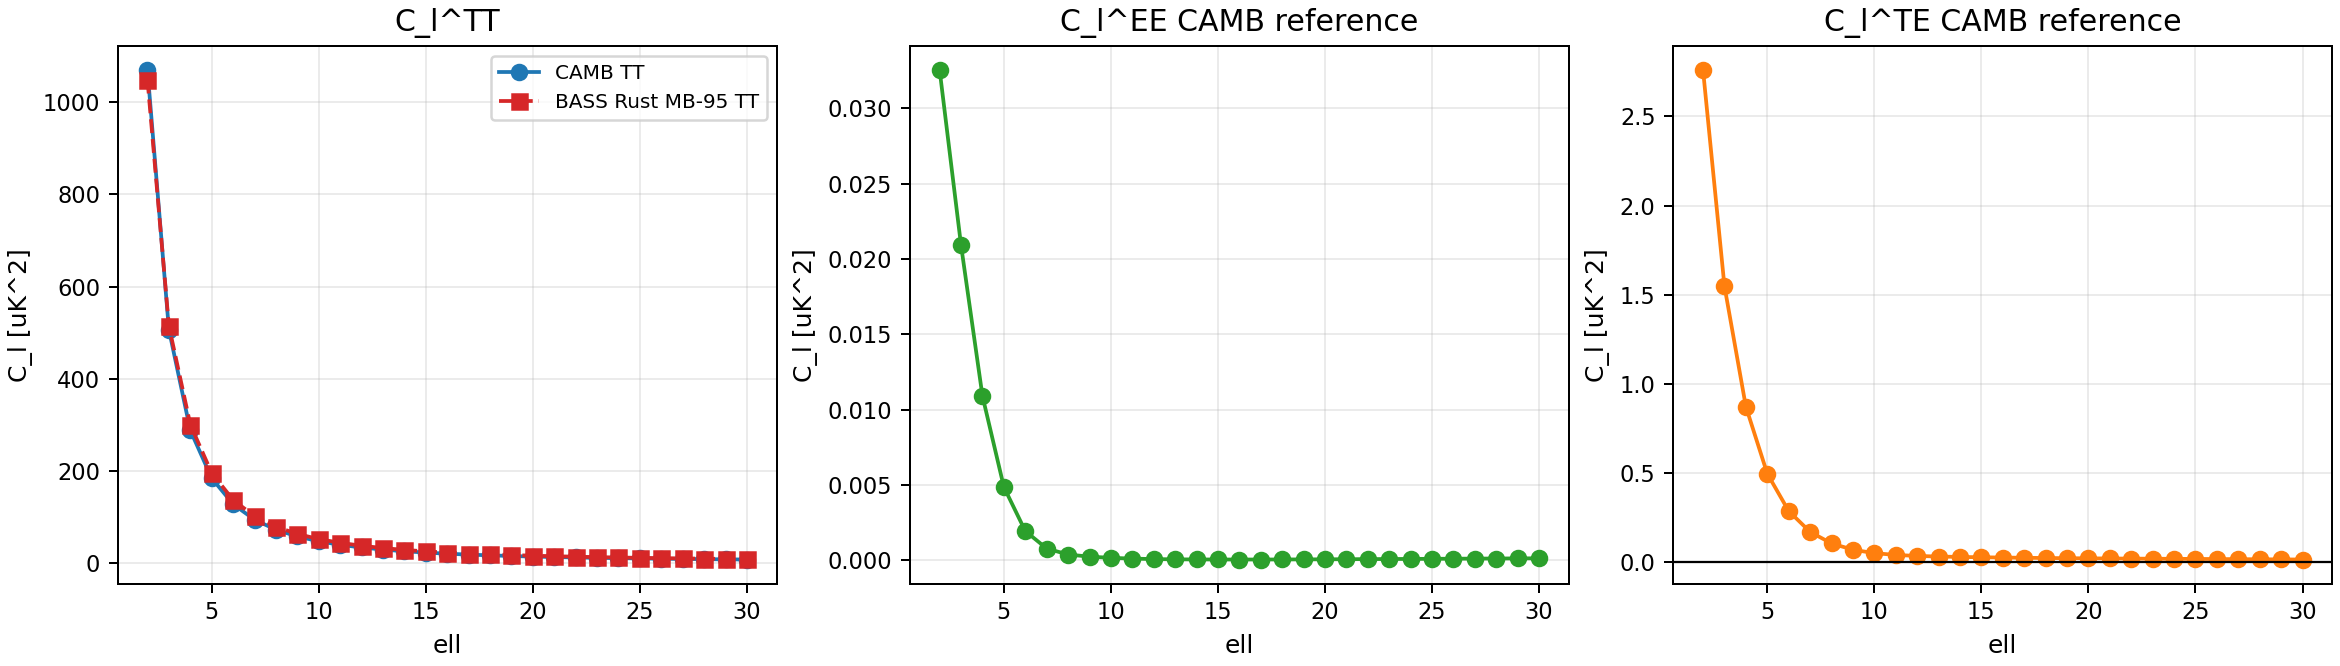
\includegraphics[width=0.82\textwidth,height=0.58\textheight,keepaspectratio]{conditioned_legacy/validation__flrw_lowell_cell_camb_bass_lmax30}
\captionof{figure}{Conditioned legacy diagnostic: flrw lowell cell camb bass lmax30. Condition: FLRW validation-context diagnostic; not anisotropic native-transfer validation. See sidecar manifest for provenance and caveats; appendix-only, not native-transfer or family-ID evidence.}
\label{fig:conditioned-legacy-validation-flrw-lowell-cell-camb-bass-lmax30}
\end{center}

\clearpage
\begin{center}
\centering
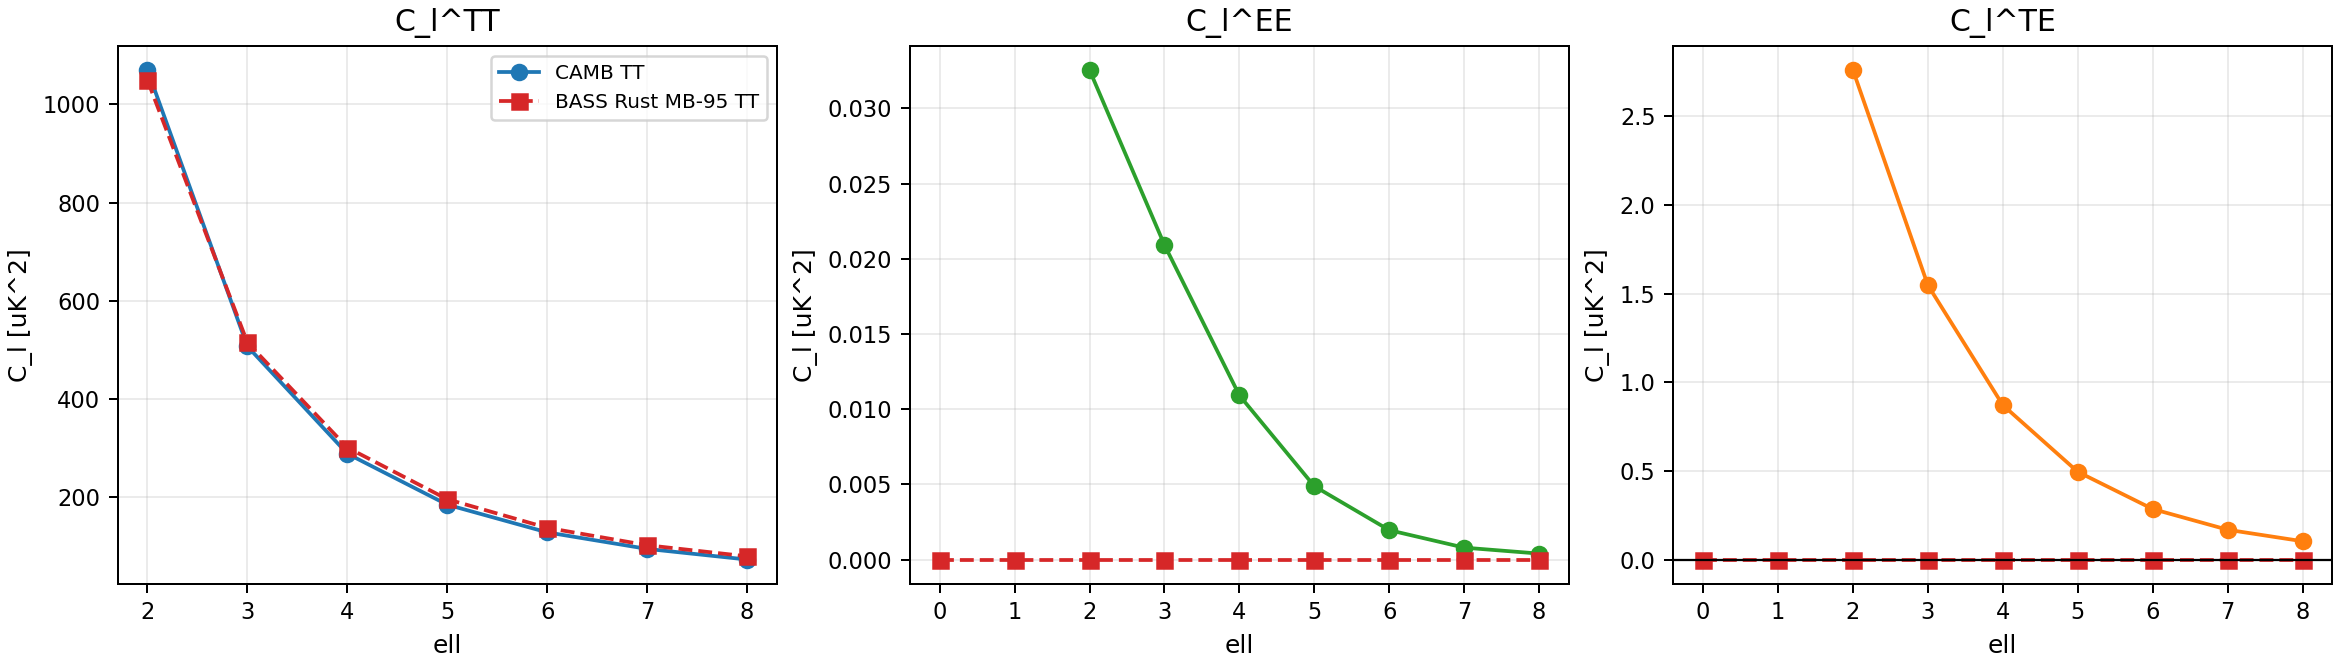
\includegraphics[width=0.82\textwidth,height=0.58\textheight,keepaspectratio]{conditioned_legacy/validation__flrw_lowell_cell_camb_bass_lmax8}
\captionof{figure}{Conditioned legacy diagnostic: flrw lowell cell camb bass lmax8. Condition: FLRW validation-context diagnostic; not anisotropic native-transfer validation. See sidecar manifest for provenance and caveats; appendix-only, not native-transfer or family-ID evidence.}
\label{fig:conditioned-legacy-validation-flrw-lowell-cell-camb-bass-lmax8}
\end{center}

\clearpage
\begin{center}
\centering
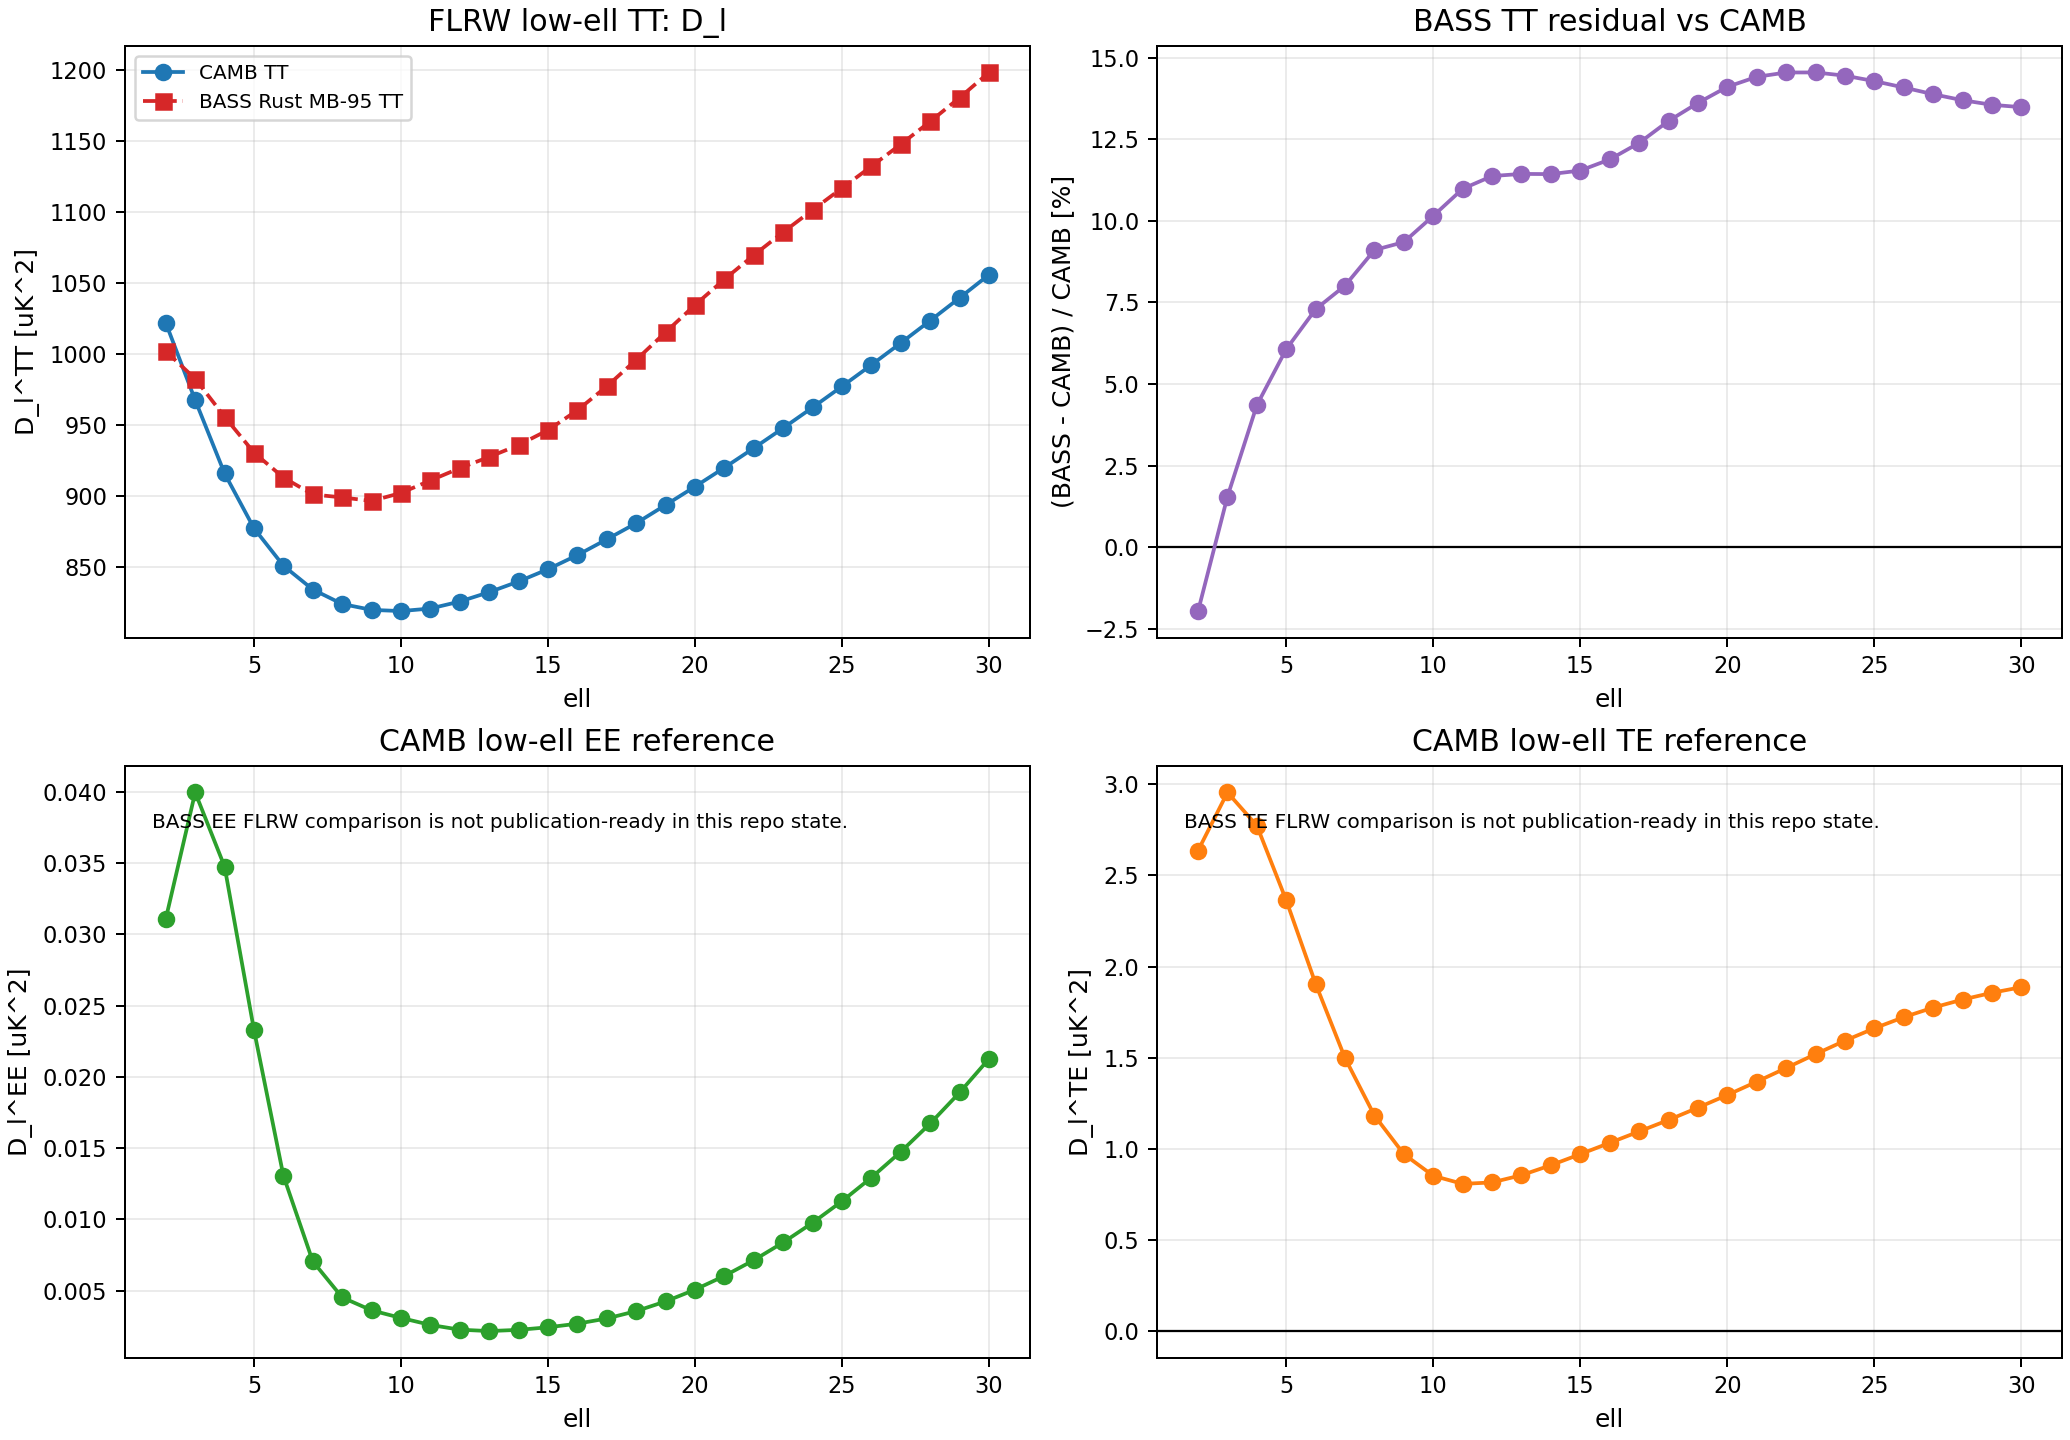
\includegraphics[width=0.82\textwidth,height=0.58\textheight,keepaspectratio]{conditioned_legacy/validation__flrw_lowell_dell_camb_bass_lmax30}
\captionof{figure}{Conditioned legacy diagnostic: flrw lowell dell camb bass lmax30. Condition: FLRW validation-context diagnostic; not anisotropic native-transfer validation. See sidecar manifest for provenance and caveats; appendix-only, not native-transfer or family-ID evidence.}
\label{fig:conditioned-legacy-validation-flrw-lowell-dell-camb-bass-lmax30}
\end{center}

\clearpage
\begin{center}
\centering
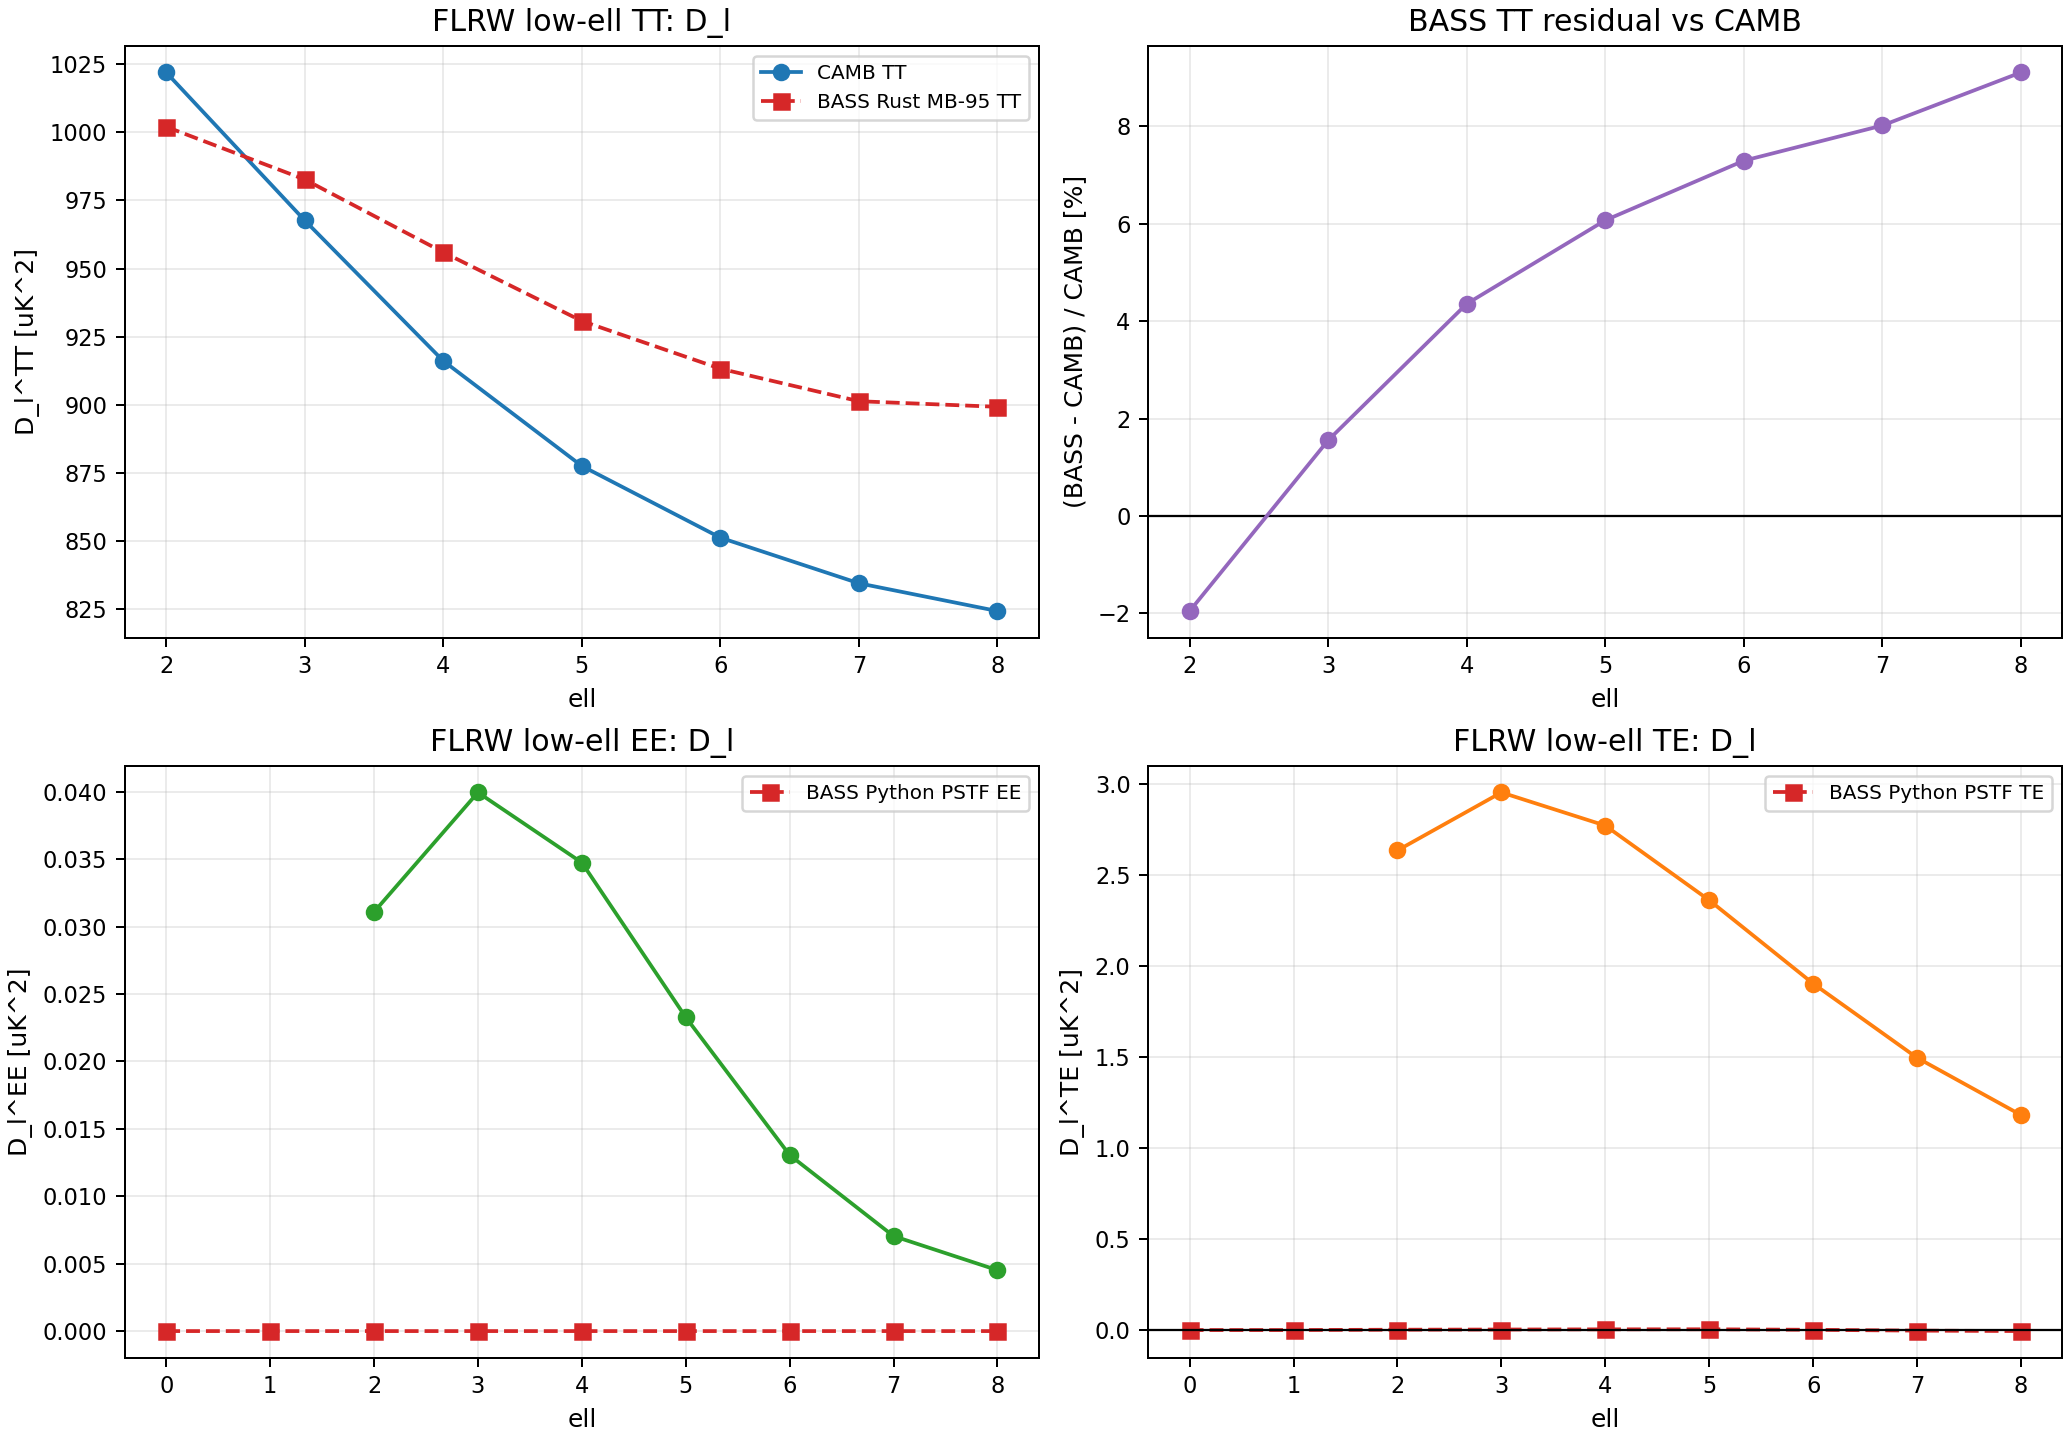
\includegraphics[width=0.82\textwidth,height=0.58\textheight,keepaspectratio]{conditioned_legacy/validation__flrw_lowell_dell_camb_bass_lmax8}
\captionof{figure}{Conditioned legacy diagnostic: flrw lowell dell camb bass lmax8. Condition: FLRW validation-context diagnostic; not anisotropic native-transfer validation. See sidecar manifest for provenance and caveats; appendix-only, not native-transfer or family-ID evidence.}
\label{fig:conditioned-legacy-validation-flrw-lowell-dell-camb-bass-lmax8}
\end{center}



% ============================================================
\chapter{Supplementary Figures}
\label{app:supp-figures}
% ============================================================

This appendix collects supplementary figures referenced in
the main text but not displayed inline.

\section{Revision diagnostic assets}
\label{app:revision-diagnostic-assets}

The figures in this section are generated by
\texttt{scripts/generate\_revision\_experiment\_assets.py} and are
manifested as paper-appendix diagnostics.  They expose support,
uncertainty, and denominator sensitivities for the revision programme;
they are not native-transfer outputs, not HTT evidence, and not
Bianchi family-identification claims.  The rule-of-three FPR panel from
the same generator is external-audit-only and is intentionally not
included in the manuscript.

% Generated by scripts/generate_revision_experiment_assets.py.
% Do not edit figure paths by hand; regenerate instead.
% Revision diagnostic appendix figures
% Contains only assets whose manifest allowed_use is paper_appendix or paper_appendix_blocked_degeneracy.

\begin{figure}[htbp]
\centering
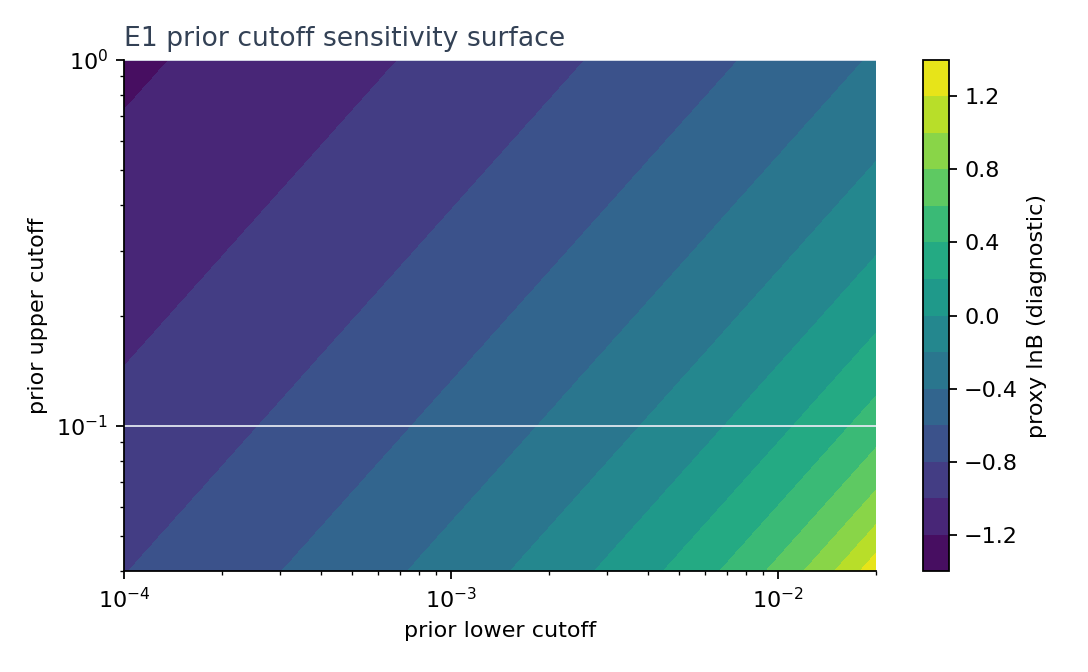
\includegraphics[width=0.92\textwidth]{current/fig_revision_prior_support_surface}
\caption{Revision appendix diagnostic prior-support surface. The plotted proxy exposes support sensitivity under the manifested prior-floor and prior-ceiling scan; it is appendix-only, diagnostic-only, not an evidence-grade Bayes factor, not native low-ell transfer output, and not a Bianchi family-ID claim.}
\label{fig:revision-prior-support-surface}
\end{figure}

\begin{figure}[htbp]
\centering
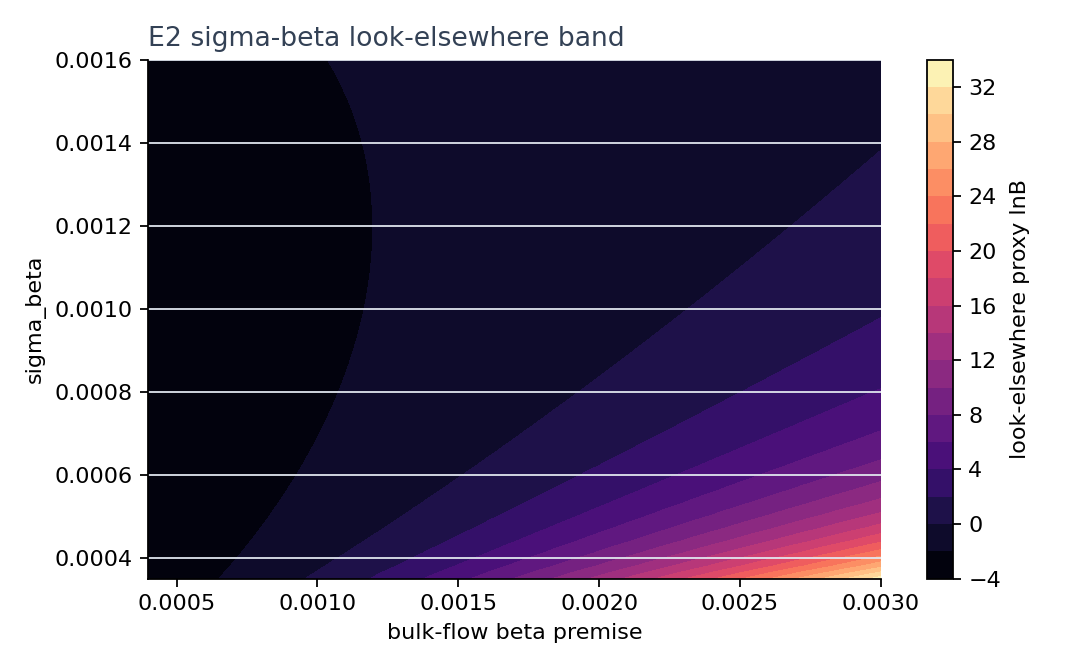
\includegraphics[width=0.92\textwidth]{current/fig_revision_sigma_beta_band}
\caption{Revision appendix diagnostic sigma-beta band. The panel records bulk-flow uncertainty sensitivity and display-only look-elsewhere bookkeeping under the current manifest; it is appendix-only, not evidence-grade support, not native-transfer validation, and not a geometry or family claim.}
\label{fig:revision-sigma-beta-band}
\end{figure}

\begin{figure}[htbp]
\centering
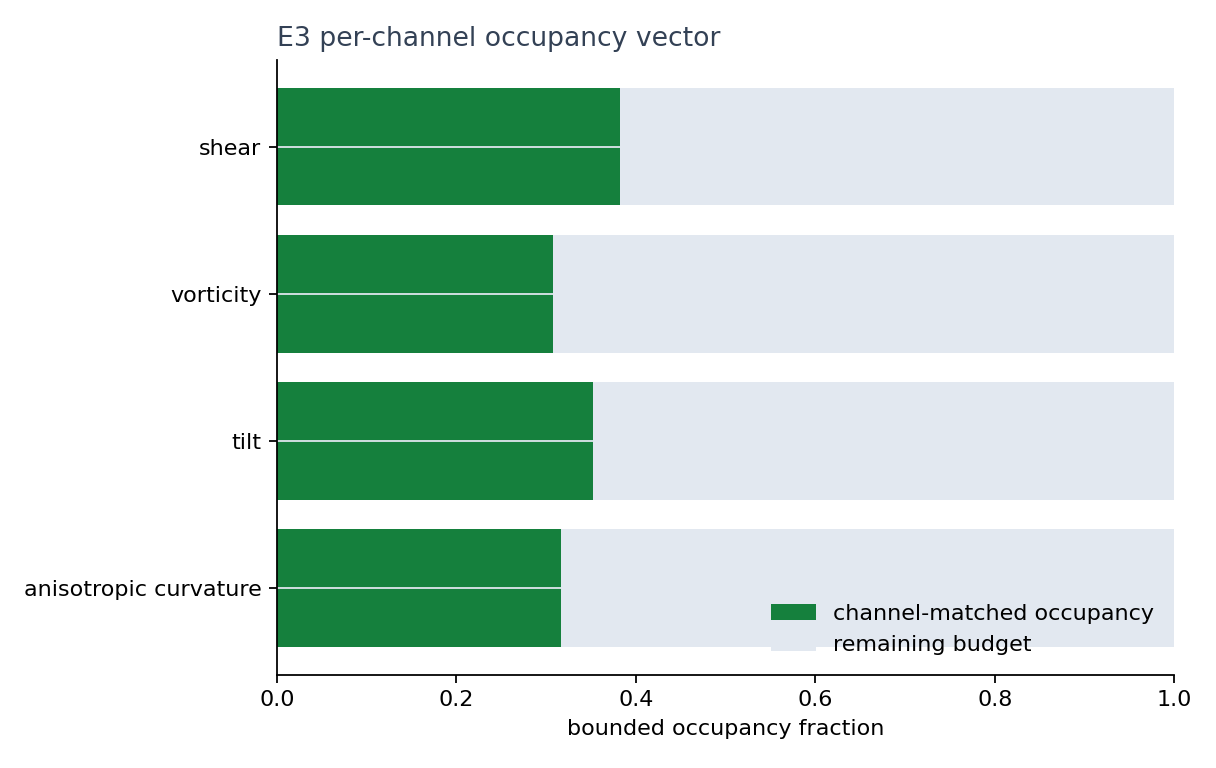
\includegraphics[width=0.92\textwidth]{current/fig_revision_per_channel_occupancy}
\caption{Revision appendix diagnostic per-channel occupancy. The bars use channel-matched proxy denominators to expose occupancy bookkeeping; scalar $Q$ remains blocked for channel mismatch and the plot does not support geometry detection or Bianchi family-ID.}
\label{fig:revision-per-channel-occupancy}
\end{figure}

\begin{figure}[htbp]
\centering
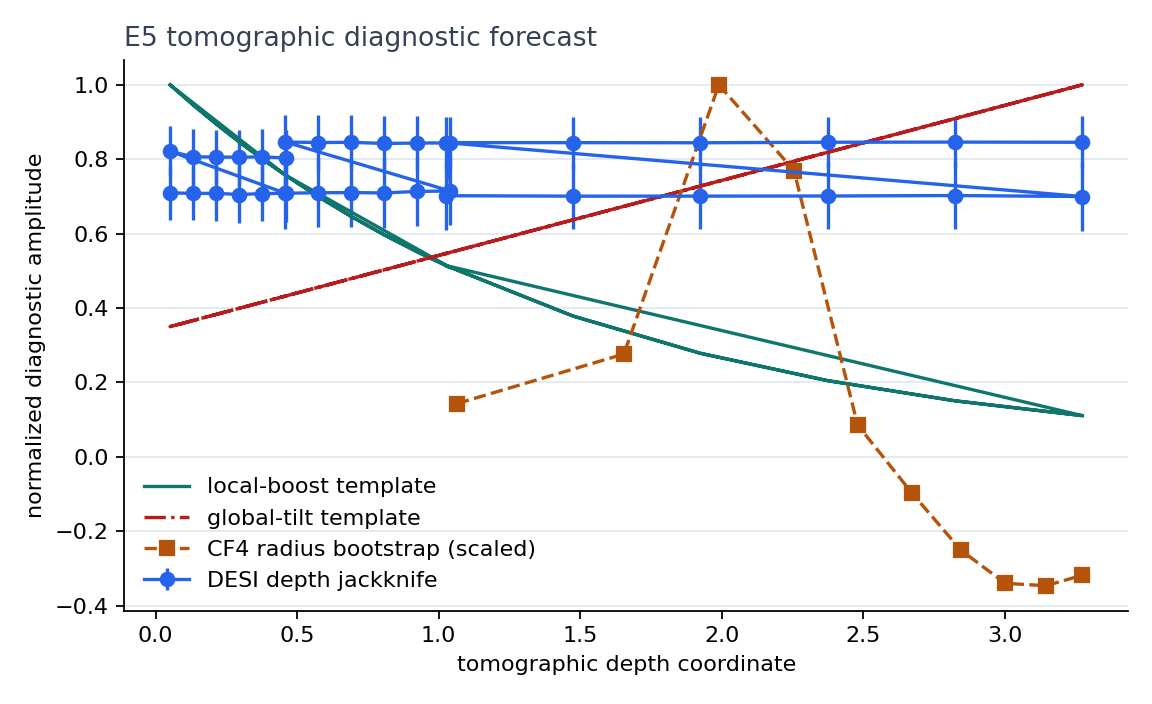
\includegraphics[width=0.92\textwidth]{current/fig_revision_tomographic_forecast}
\caption{Revision appendix blocked-degeneracy tomographic forecast. The manifest records a forecast-only local/global template-rank design with jackknife/bootstrap diagnostic status; the local-boost and global-tilt depth templates are near-degenerate, so this is a methods negative result, not a paper-main candidate. It is diagnostic-only and remains conditioned on blocked native-atlas status, matched covariance, and external null gates.}
\label{fig:revision-tomographic-forecast}
\end{figure}


\section{x/F/G/Pi theorem-extension diagnostics}
\label{app:theorem-extension-diagnostics}

The figures in this section are generated by
\texttt{scripts/generate\_theorem\_extension\_assets.py} from
synthetic/manufactured theorem-helper inputs.  They are
appendix-only diagnostics for x/F/G/Pi theorem-extension
obligations, EGS/Boltzmann extension gates, and kill-switch
surfaces.  They are not HTT evidence, not MIO certificates, not
native-transfer outputs, and not geometry or family-identification
support.

% Generated by scripts/generate_theorem_extension_assets.py.
% Do not edit figure paths by hand; regenerate instead.
% Theorem extension appendix figures.
% Contains only assets whose manifest allowed_use is paper_appendix.

\begin{figure}[htbp]
\centering
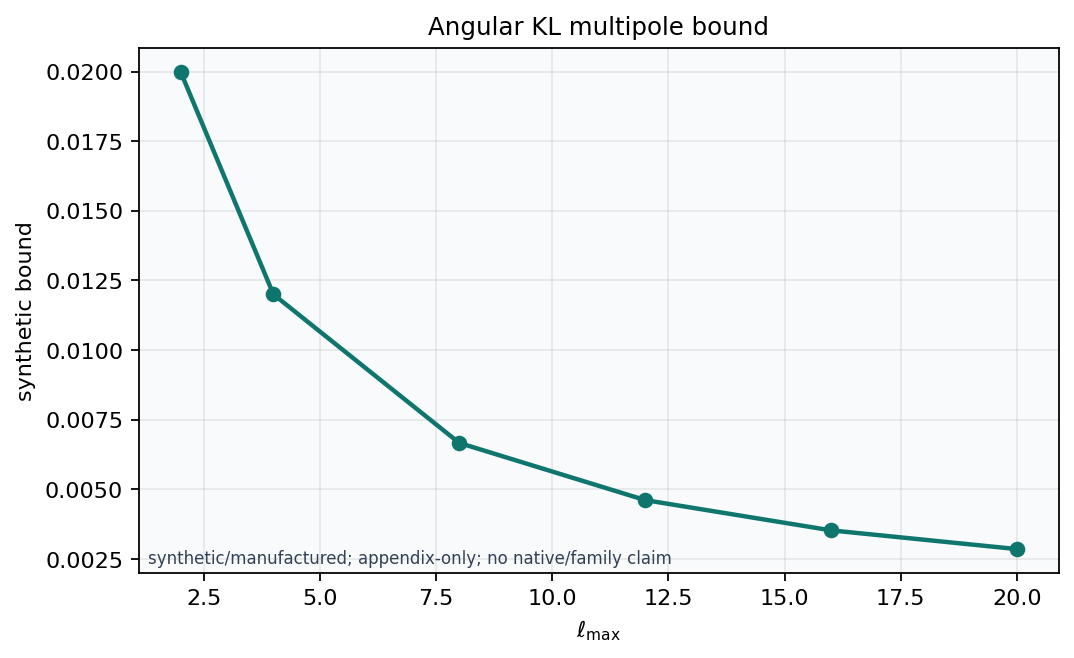
\includegraphics[width=0.92\textwidth]{current/fig_theorem_angular_kl_bound}
\caption{Appendix-only synthetic angular KL multipole bound. The panel shows a manufactured density-fixture scaling and remains diagnostic-only; it is not HTT evidence, not a MIO certificate, not native solver validation, and not geometry or family identification.}
\label{fig:theorem-angular-kl-bound}
\end{figure}

\begin{figure}[htbp]
\centering
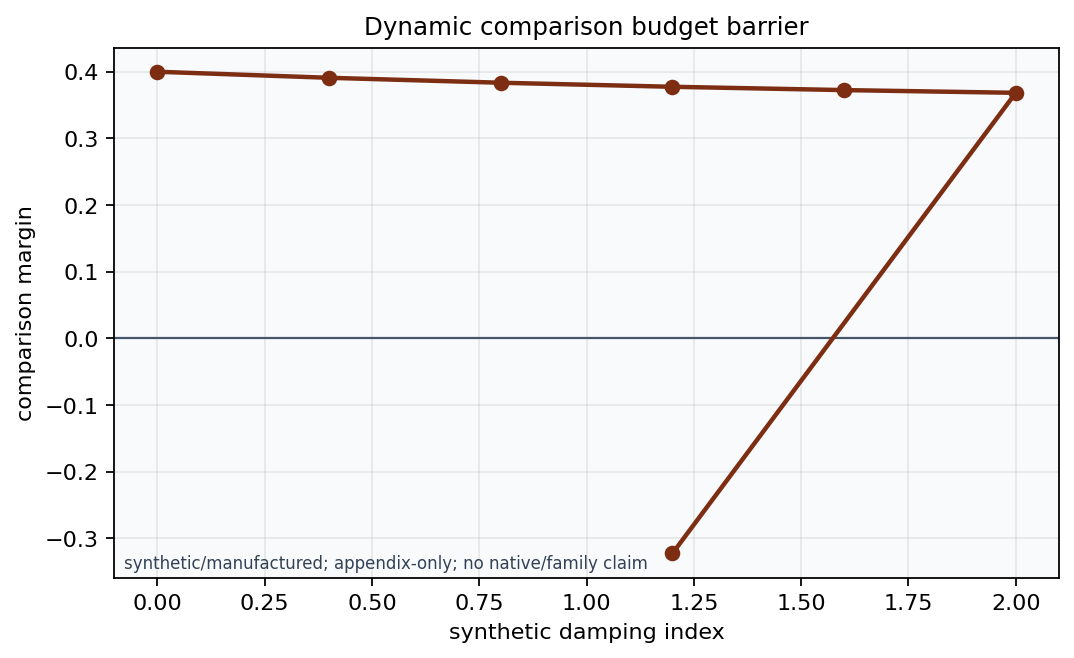
\includegraphics[width=0.92\textwidth]{current/fig_theorem_dynamic_budget_barrier}
\caption{Appendix-only synthetic dynamic budget barrier. The plotted margin is a same-channel manufactured comparison diagnostic; it is not HTT evidence, not a MIO certificate, not native solver validation, and not geometry or family identification.}
\label{fig:theorem-dynamic-budget-barrier}
\end{figure}

\begin{figure}[htbp]
\centering
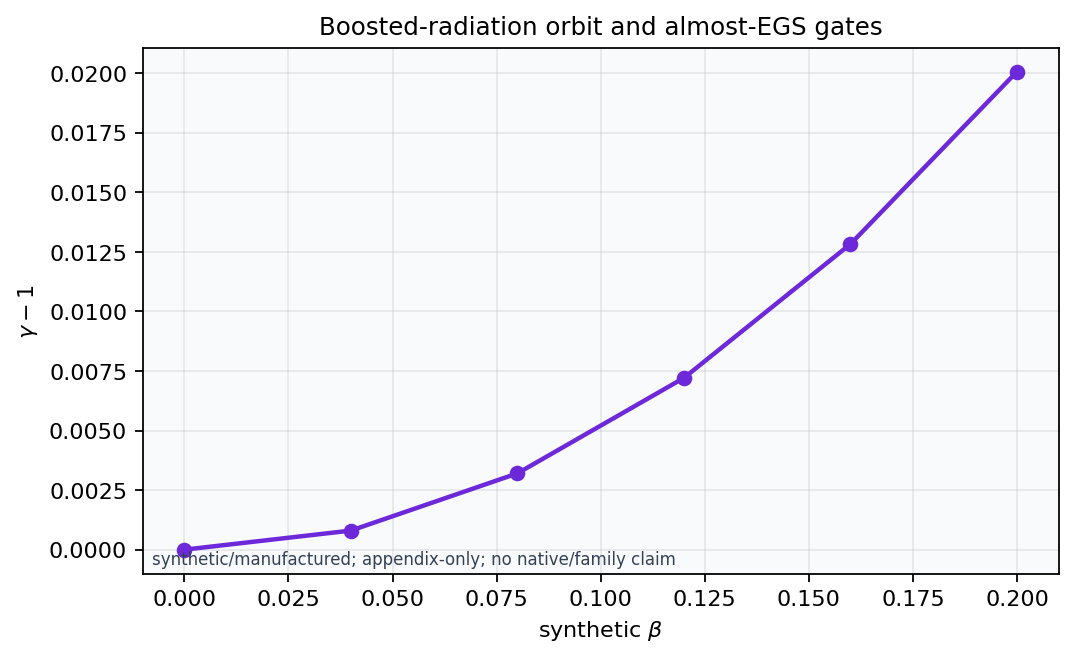
\includegraphics[width=0.92\textwidth]{current/fig_theorem_boosted_radiation_orbit}
\caption{Appendix-only synthetic boosted-radiation orbit gate. The curve is a manufactured Lorentz-orbit diagnostic and the data-facing residual gate remains blocked; it is not HTT evidence, not a MIO certificate, not native solver validation, and not geometry or family identification.}
\label{fig:theorem-boosted-radiation-orbit}
\end{figure}

\begin{figure}[htbp]
\centering
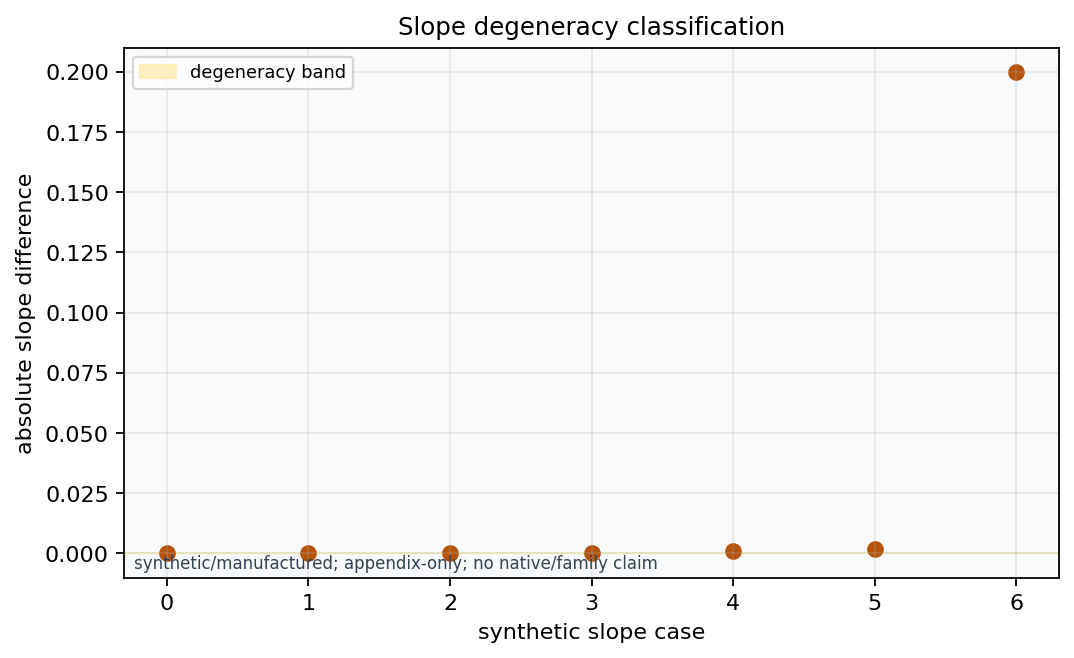
\includegraphics[width=0.92\textwidth]{current/fig_theorem_slope_degeneracy}
\caption{Appendix-only synthetic slope-degeneracy gate. The shaded band marks manufactured slope-only degeneracy, which blocks source discrimination; it is not HTT evidence, not a MIO certificate, not native solver validation, and not geometry or family identification.}
\label{fig:theorem-slope-degeneracy}
\end{figure}

\begin{figure}[htbp]
\centering
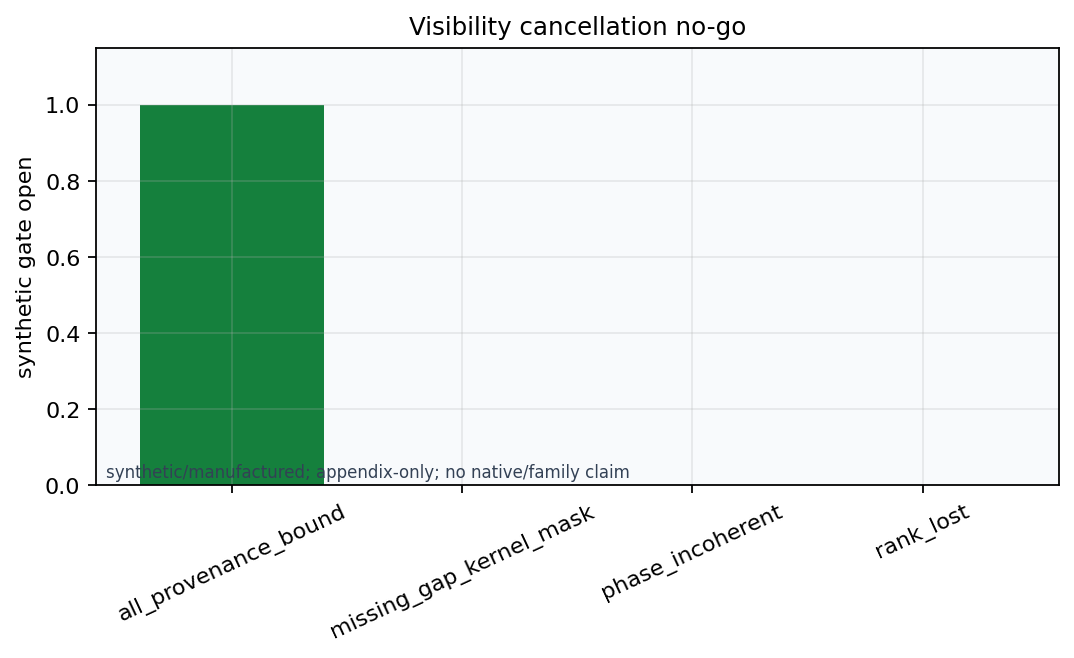
\includegraphics[width=0.92\textwidth]{current/fig_theorem_visibility_cancellation}
\caption{Appendix-only synthetic visibility-cancellation gate. The bars show manufactured fail-closed source upper-bound conditions; it is not HTT evidence, not a MIO certificate, not native solver validation, and not geometry or family identification.}
\label{fig:theorem-visibility-cancellation}
\end{figure}


\subsection{EGS-type low-$\ell$ diagnostic theorems (NT-A1, NT-A3,
NT-B3)}\label{sec:egs-lowell-theorems}

The following three conditional theorems carry the
Ehlers--Geren--Sachs (EGS) chain onto the report's diagnostic
variables $F$, $Q$, $\Pi$, and the depth gap $G_F$.  Each is a
structural or limiting statement under explicitly stated
hypotheses---not a detection---and each algebraic step, limit, and
variance propagation was verified symbolically with the Wolfram
Engine; the machine-checked proof record is
\texttt{docs/generated/egs\_lowell\_theorem\_proofs.json}.  We write
the temperature-quadrupole magnitude $a_2$, the shear scalar
$\Sigma$, the quadrupole power $D_2\propto a_2^2$, the algebraic
ceiling $x_{\max}$, and the shear filling $F_{\rm shear} =
\Sigma^2/x_{\max}$.

\begin{theorem}[Quadrupole--filling EGS-type identity]\label{thm:nt-a1}
Assume the free-streaming linear $\ell=2$ closure $a_2 = \kappa\,
\Sigma$ with $\kappa>0$ constant (the Ehlers--Treciokas--Matravers
coefficient $\kappa = 4/21$), $F_{\rm shear} = \Sigma^2/x_{\max}$,
and $D_2 = c_D\,a_2^2$ with $c_D>0$, and that the tilt rapidity
enters the dipole $a_1$ only.  Then
\begin{equation}
F_{\rm shear} = \frac{a_2^2}{\kappa^2\,x_{\max}}
  = \frac{D_2}{c_D\,\kappa^2\,x_{\max}} \;\propto\; D_2,
\end{equation}
so $F_{\rm shear}\to 0$ as $D_2\to 0$ (the EGS limit: an isotropic
CMB forces zero shear-filling), and $\partial F_{\rm shear}/\partial
\beta = 0$ (the tilt sector is invisible to the shear-filling).
\end{theorem}

\noindent\emph{Proof.} Substitute $\Sigma = a_2/\kappa$ into $F_{\rm
shear}=\Sigma^2/x_{\max}$ and $a_2=\sqrt{D_2/c_D}$; the limit and
the $\beta$-derivative are immediate.  The $\ell=2$ projection that
licenses the closure rests on the sphere averages $\langle
n_a n_b\rangle = \tfrac13\delta_{ab}$ (Wolfram-verified).
Conditional on the free-streaming linear closure. $\square$

\begin{theorem}[Cosmic-variance Cram\'er--Rao floor on
$F_{\rm shear}$]\label{thm:nt-a3}
Under Theorem~\ref{thm:nt-a1}, $F_{\rm shear}$ is linear in the
quadrupole power $C_2$.  With the single-sky cosmic variance
$\mathrm{Var}(C_2) = 2\,C_2^2/(2\ell+1)$ ($\chi^2$ with $2\ell+1$
degrees of freedom),
\begin{equation}
\frac{\sigma(F_{\rm shear})}{F_{\rm shear}}
  \;\ge\; \sqrt{\frac{2}{2\ell+1}}
  \;\xrightarrow{\ \ell=2\ }\; \sqrt{\tfrac{2}{5}} \approx 0.632 .
\end{equation}
Hence the shear-filling fraction cannot be measured to better than
$\sim 63\%$ fractional precision from a single-sky quadrupole.
\end{theorem}

\noindent\emph{Proof.} Error propagation $\mathrm{Var}(F_{\rm
shear}) = (\partial F_{\rm shear}/\partial C_2)^2\,\mathrm{Var}(C_2)
= \tfrac{2}{2\ell+1}\,F_{\rm shear}^2$; take the square root and set
$\ell=2$ (Wolfram-verified). $\square$

\begin{theorem}[Depth-transport EGS limit for
$G_F$]\label{thm:nt-b3}
Write the depth-resolved filling additively, $F(z) = F_{\rm
shear}(z) + F_{\rm tilt}(z)$, and the depth gap $G_F(z) =
F(z)/F(z_{\rm ref})$.  For a depth-steady shear with no tilt,
$G_F(z)\equiv 1$ (the EGS depth limit: no depth gap); a
depth-evolving tilt imprints a nonzero $\mathrm{d}G_F/\mathrm{d}z$.
\end{theorem}

\noindent\emph{Proof.} With $F_{\rm tilt}\equiv 0$ and $F_{\rm
shear}$ constant in $z$, $G_F = F_{\rm shear}/F_{\rm shear} = 1$ and
$\mathrm{d}G_F/\mathrm{d}z = 0$; a power-law tilt $F_{\rm tilt} = c\,
z^{q}$ gives $\mathrm{d}G_F/\mathrm{d}z = c\,q\,z^{q-1}/(F_{\rm
shear} + c\,z_{\rm ref}^{q}) \neq 0$ (Wolfram-verified).
Conditional on the additive decomposition. $\square$

These statements are diagnostic-only program theorems: they do not
constitute HTT evidence, MIO certificates, native low-$\ell$ solver
output, geometry-detection, or Bianchi family-ID, and the closure
coefficient $\kappa$ and the observational mapping to the measured
Planck $D_2$ remain the stated conditioning.

\begin{figure}[ht]
\centering
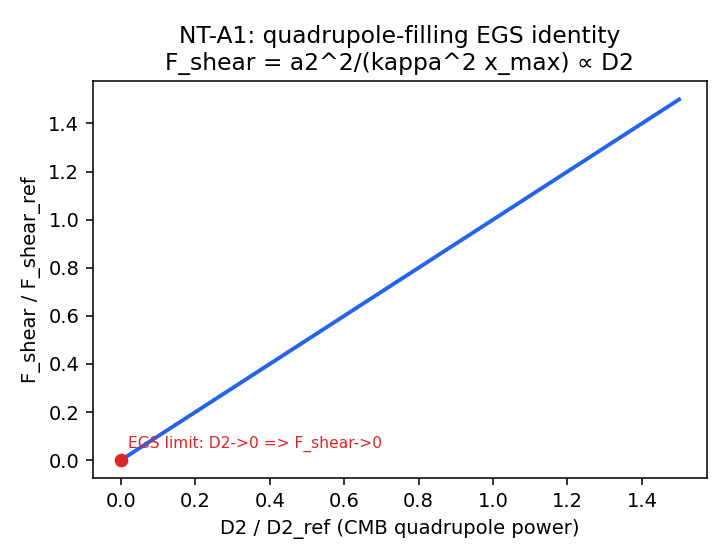
\includegraphics[width=0.78\textwidth]{current/fig_theorem_nt_a1_quadrupole_filling}
\caption{Theorem~\ref{thm:nt-a1} (NT-A1): the shear filling fraction
is linear in the CMB quadrupole power $D_2$ and vanishes in the EGS
limit $D_2\to 0$.  Diagnostic-only analytic illustration; not a
detection.}
\label{fig:theorem-nt-a1-quadrupole-filling}
\end{figure}

\begin{figure}[ht]
\centering
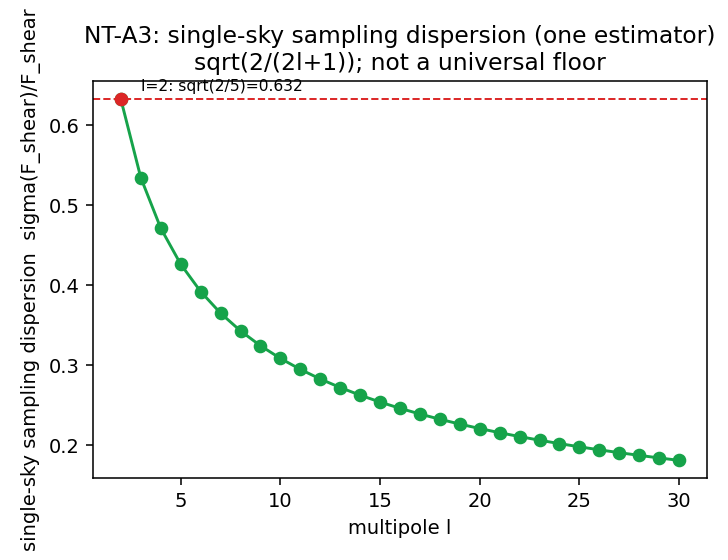
\includegraphics[width=0.78\textwidth]{current/fig_theorem_nt_a3_cosmic_variance_floor}
\caption{Theorem~\ref{thm:nt-a3} (NT-A3): the cosmic-variance
fractional floor $\sqrt{2/(2\ell+1)}$ on $F_{\rm shear}$, equal to
$\sqrt{2/5}\approx 0.632$ at the quadrupole.  Diagnostic-only;
not a detection.}
\label{fig:theorem-nt-a3-cosmic-variance-floor}
\end{figure}

\begin{figure}[ht]
\centering
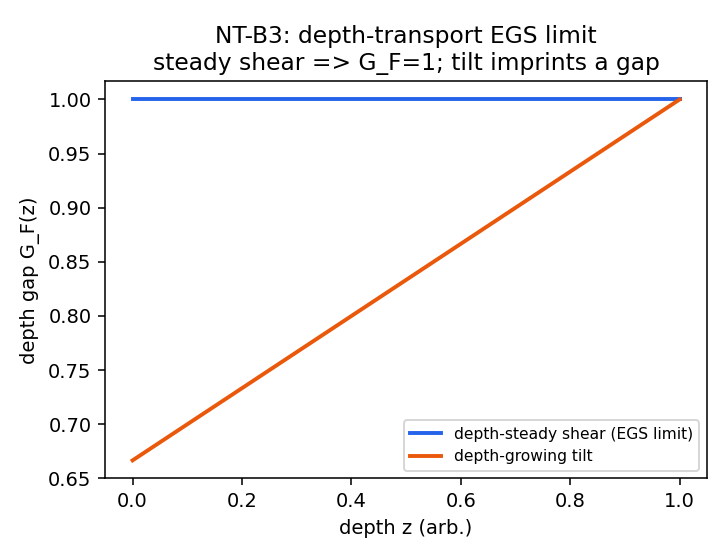
\includegraphics[width=0.78\textwidth]{current/fig_theorem_nt_b3_gf_transport}
\caption{Theorem~\ref{thm:nt-b3} (NT-B3): the depth gap $G_F(z)$ is
flat at unity for a depth-steady shear (EGS depth limit) and rises
when a depth-evolving tilt is present.  Diagnostic-only; not a
detection.}
\label{fig:theorem-nt-b3-gf-transport}
\end{figure}

\bibliographystyle{plainnat}
\bibliography{references}

\end{document}
